\documentclass[
openright,
12pt, % The default document font size, options: 10pt, 11pt, 12pt
%oneside, % Two side (alternating margins) for binding by default, uncomment to switch to one side
english,% ngerman for German
onehalfspacing, %singlespacing: Single line spacing, alternatives: onehalfspacing or doublespacing
%draft, % Uncomment to enable draft mode (no pictures, no links, overfull hboxes indicated)
nolistspacing, % If the document is onehalfspacing or doublespacing, uncomment this to set spacing in lists to single
%liststotoc, % Uncomment to add the list of figures/tables/etc to the table of contents
%toctotoc, % Uncomment to add the main table of contents to the table of contents
%parskip, % Uncomment to add space between paragraphs
nohyperref, % Uncomment to not load the hyperref package
headsepline, % Uncomment to get a line under the header
%chapterinoneline, % Uncomment to place the chapter title next to the number on one line
%consistentlayout, % Uncomment to change the layout of the declaration, abstract and acknowledgements pages to match the default layout\\
]{MastersDoctoralThesis} % The class file specifying the document structure

%\usepackage[a-2b,mathxmp]{pdfx}[2018/12/22] %To generate a PDF/A compatible document for longterm archiving (see ../documents/)

%% ------------ 
%% FONT 
%% ------------

\usepackage[T1]{fontenc} % Output font encoding for international characters
\usepackage[utf8]{inputenc} % Required for inputting international characters
% \usepackage{mathpazo} % Use the Palatino font by default

%% ------------
%%  Bibliography
%% ------------

\usepackage[
backend=bibtex,
style=authoryear-comp,
natbib=true,
sorting=debug,
maxnames=1,
uniquelist=true]{biblatex} % Use the bibtex backend with the (options:numeric-comp,authoryear-comp,firstinits=true) citation style (which resembles APA)

\addbibresource{../references} % references for the thesis

\usepackage[autostyle=true]{csquotes} % Required to generate language-dependent quotes in the bibliography
\usepackage{pdfpages}


%----------------------------------------------------------------------------------------
%    MARGIN SETTINGS
%----------------------------------------------------------------------------------------
%\usepackage{layouts} for getting \textwidth \linewidth in human readable units
\geometry{
    paper=a4paper, % Change to letterpaper for US letter
    top=2.35cm, % Top margin
    bottom=2.35cm, % Bottom margin
    left=3.2765cm,
    right=2.32cm,
    %width=16cm, %width of the text
    %inner=2.5cm, % Inner margin
    %outer=3.8cm, % Outer margin
    %bindingoffset=.6cm, % Binding offset    
    %showframe, % Uncomment to show how the type block is set on the page
}

\captionsetup{width=\textwidth}

%----------------------------------------------------------------------------------------
%    USER-SPECIFIC PACKAGES
%----------------------------------------------------------------------------------------

\usepackage{color}
\usepackage{xcolor}
\usepackage{acronym}
\usepackage{booktabs}
\usepackage{dcolumn}
\usepackage{graphicx}
\usepackage{amsmath,amsfonts,amssymb}
\usepackage{mathrsfs}
\usepackage{mathtools}
\usepackage[normalem]{ulem}
\usepackage{graphicx,psfrag}
\usepackage{mathrsfs}
%\usepackage{amsmath,amsfonts,amssymb}%%\usepackage{amsmath}
\usepackage{multirow}
\usepackage{comment}
\usepackage{ulem}
\usepackage{colortbl} % for fit tables colored rows
\usepackage{pifont} % \cmark \xmark % http://ctan.org/pkg/pifont
\usepackage[breaklinks,colorlinks,citecolor=blue]{hyperref}
\newcommand{\cmark}{\ding{51}}%
\newcommand{\xmark}{\ding{55}}%
\usepackage{rotating}
\usepackage{lscape}
%\usepackage{pdflscape}
\usepackage{afterpage}
\usepackage{capt-of}% or use the larger `caption` package
\usepackage{lipsum}% 

%----------------------------------------------------------------------------------------
%    USER-SPECIFIC DECLARATIONS AND COMMANDS
%----------------------------------------------------------------------------------------

\DeclareOldFontCommand{\rm}{\normalfont\rmfamily}{\mathrm}
\DeclareOldFontCommand{\sf}{\normalfont\sffamily}{\mathsf}
\DeclareOldFontCommand{\tt}{\normalfont\ttfamily}{\mathtt}
\DeclareOldFontCommand{\bf}{\normalfont\bfseries}{\mathbf}
\DeclareOldFontCommand{\it}{\normalfont\itshape}{\mathit}
\DeclareOldFontCommand{\sl}{\normalfont\slshape}{\@nomath\sl}
\DeclareOldFontCommand{\sc}{\normalfont\scshape}{\@nomath\sc}
\DeclareRobustCommand*\cal{\@fontswitch\relax\mathcal}
\DeclareRobustCommand*\mit{\@fontswitch\relax\mathnormal}

\newcommand{\myhead}[1]{\multicolumn{1}{c}{#1}}
\newcolumntype{d}[1]{D{.}{.}{#1}}

\graphicspath{{/home/vsevolod/GIT/GitHub/phd_thesis/v3/Figures/}}

\newcommand{\todo}[1]{\textcolor{red}{$\blacksquare$ TODO: #1}} 
\newcommand{\red}[1]{\textcolor{red}{#1}} 
\newcommand{\gray}[1]{\textcolor{gray}{#1}} 
\newcommand{\magenta}[1]{\textcolor{magenta}{#1}} %% For terms/concepts to remember 
\newcommand{\swind}{spiral-wave wind}
\newcommand{\nwind}{$\nu$-component}
\newcommand{\gcm}{g cm$^{-3}$}
\def\igscm{{\rm cm^{2}\,g^{-1}}}
\newcommand{\dd}{\text{d}}
\newcommand{\Mmax}{\ensuremath{M_\text{max}^\text{TOV}}} % High-q paper

\newcommand{\GW}{GW170817}
\newcommand{\AT}{AT2017gfo} %{{SSS17a}} %{{AT170817A}} % AT2017gfo
\newcommand{\GRB}{GRB170817A}

\newcommand{\eff}{\mathrm{eff}}
\newcommand{\cf}{\textit{cf.}}
\newcommand{\ie}{\textit{i.e.}}
\newcommand{\eg}{\textit{e.g.}}
\newcommand{\pz}{\phantom{0}}
\newcommand{\SNR}{\mathrm{SNR}}

\newcommand{\rproc}{$r$-process}
\newcommand{\sproc}{$s$-process}
\newcommand{\pmerg}{post-merger}
\newcommand{\mr}{mass ratio}
\newcommand{\nuc}{nucleosynthesis}
\newcommand{\wisky}{\texttt{WhiskyTHC}}
\newcommand{\bnc}{bounce} %% or re-bounce
\newcommand{\trans}{trans-relativistic}
\newcommand{\blast}{blast wave}
\newcommand{\mm}{multi-messenger}
\newcommand{\polql}{$P_2^2(q,\tilde{\Lambda})$}
\newcommand{\polq}{$P_2^1(\tilde{\Lambda})$}

\newcommand{\ndef}[1]{\textbf{#1}} %% for new definitions 

\def\Msun{{\text{M}_{\odot}}}
\def\Rsun{{\text{R}_{\odot}}}
\def\md{M^{\text{d}}_{\text{ej}}}
\def\vd{v^{\text{d}}_\infty}
\def\yd{Y^{\text{d}}_{e}}
\def\amd{\md}
\def\avd{\langle\vd\rangle}
\def\ayd{\langle\yd\rangle}
\def\thetarms{\theta_{\rm RMS}}
\def\athetarms{\langle\thetarms\rangle}
\def\nism{n_{\text{ISM}}}
% spiral-wind
\def\mw{M^{\text{w}}_{\text{ej}}}
\def\vw{v^{\text{w}}_\infty}
\def\yw{Y^{\text{w}}_{e}}
\def\amw{\mw}
\def\avw{\langle\vw\rangle}
\def\ayw{\langle\yw\rangle}
% nu-wind
\def\mnu{M^{\nu\text{w}}_{\text{ej}}}
\def\vnu{v^{\nu\text{w}}_\infty}
\def\ynu{Y^{\nu\text{w}}_e}
\def\amnu{\mnu}
\def\avnu{\langle\vnu\rangle}
\def\aynu{\langle\ynu\rangle}

\def\ccm{\,\text{cm}^{-3}}


%----------------------------------------------------------------------------------------
%    USER-SPECIFIC ACRONYMS (IF ANY)
%----------------------------------------------------------------------------------------
%\newacro{KH}{Kelvin-Helmholtz} %% NEVER USE IT! WILL BREACK YOUR LATEX
\newacro{KHI}{Kelvin-Helmholtz instability}
\newacro{MRI}{magnetorotational instability}

\newacro{BH}{black hole}
\newacro{BBH}{binary black-hole}
\newacro{BHNS}{black-hole neutron-star}
\newacro{BNS}{binary neutron star}
\newacro{EM}{electromagnetic}
\newacro{EOS}{equation of state}
\newacroplural{EOS}[EOSs]{equations of state}
\newacro{GR}{general relativity}
\newacro{HD}{hydrodynamics}
\newacro{MHD}{magnetohydrodynamics}
\newacro{GRLES}{general-relativistic large-eddy simulation}
\newacro{GRHD}{general-relativistic hydrodynamics}
\newacro{GRMHD}{general-relativistic magnetohydrodynamics}
\newacro{GW}{gravitational wave}
\newacroplural{GW}[GWs]{gravitational waves}
\newacro{LES}{large-eddy simulation}
\newacroplural{LES}[LES]{large-eddy simulations}
\newacro{GRLES}{general-relativistic large-eddy simulation}
\newacro{NR}{numerical relativity}
\newacro{NS}{neutron star}
\newacroplural{NS}[NSs]{neutron stars}
\newacro{GRB}{$\gamma$-ray burst}
\newacro{SGRB}{short $\gamma$-ray burst}
\newacro{ISM}{interstellar medium}
\newacro{MNS}{massive neutron star}
\newacro{NSBH}{neutron star-black hole}
\newacro{NSE}{nuclear statistical equilibrium}
\newacro{SN}{supernova}
\newacroplural{SN}[SNe]{supernovae}
\newacro{CCSN}{core-collapse supernova}
\newacroplural{CCSN}[CCSNe]{Core-collapse supernovae}
\newacro{BBN}{Big Bang nucleosynthesis}
\newacro{MP}{metal-poor}
\newacro{AGB}{asymptotic giant branch}
\newacro{UFG}{ultra-faint dwarf galaxy}
\newacroplural{UFG}[UFGs]{ultra-faint dwarf galaxies}
\newacro{NRN}{nuclear reaction network}
\newacroplural{NRN}[NRNs]{nuclear reaction networks}
\newacro{kN}{kilonova}
\newacroplural{kN}[kNe]{kilonovae}
\newacro{RR}{reaction rate}
\newacroplural{RR}[RRs]{reaction rates}
\newacro{MBD}{Maxwell-Boltzmann distribution}
\newacro{CS}{cross-section}
\newacro{ODE}{ordinary differential equation}
\newacroplural{ODE}[ODEs]{ordinary differential equations}
\newacro{RK}{Runge-Kutta}
\newacro{SPH}{smoothed particle hydrodynamics}
\newacro{IR}{infrared}
\newacro{NIR}{near-infrared}
\newacro{LC}{light curve}
\newacroplural{LC}[LCs]{light curves}
\newacro{UV}{ultraviolet}
\newacro{LTE}{local thermodynamic equilibrium}
\newacro{TOV}{Tolman-Oppenheimer-Volkoff}
\newacro{AH}{apparent horizon}
\newacro{RMS}{root mean square}
\newacro{MM}{multi-messenger}
\newacro{LK}{light curve}
\newacro{IC}{Inverse Compton}
\newacro{CBM}{circumburst medium}
\newacro{LF}{Lorentz factor}
\newacro{DF}{Doppler factor}
\newacro{SSC}{synchrotron self-Compton}
\newacro{SSA}{synchrotron self-absorption}
\newacro{CoE}{center of explostion}
\newacro{FS}{forward shock}
\newacro{RS}{reverse shock}
\newacro{EFE}{Einstein’s field equations}
\newacro{ADM}{Arnowitt, Deser and Misner}
\newacro{IVP}{initial value problem}
\newacro{RHS}{right hand side}
\newacro{CTS}{conformal thin-sandwich} 
\newacro{RMF}{relativistic mean-field}
\newacro{BTE}{Boltzmann transport equation}
\newacro{FV}{finite-volume}
\newacro{FD}{finite-difference}%{finite-differencing}
\newacro{HRSC}{high-resolution shock-capturing}
\newacro{CFL}{Courant-Friedrichs-Lewy}
\newacro{TVD}{total-variation diminishing}
\newacro{BV}{bounded variation}
\newacro{TV}{total variation}
\newacro{PPM}{piecewise parabolic method}
\newacro{PHM}{piecewise hyperbolic method}
\newacro{ENO}{essentially non-oscillatory}
\newacro{WENO}{weighted essentially non-oscillatory}
\newacro{MP5}{monotonicity-preserving}
\newacro{HLLE}{Harten, Lax, van Leer and Einfeldt}
\newacro{HLLC}{Harten-Lax-van Leer-Contact}
\newacro{LxF}{Lax and Friedrichs}
\newacro{NT}{Nessyahu and Tadmor}
\newacro{KT}{Kurganov and Tadmor}
\newacro{AMR}{adaptive mesh refinement}
\newacro{PPL}{positivity preserving limiter}
\newacro{SSP}{strong stability preserving}
\newacro{PDE}{partial differential equation}
\newacroplural{PDE}[PDEs]{partial differential equations}
\newacro{MOL}{method of lines}
\newacro{EM}{electromagnetic}
\newacro{HMNS}{hyper-massive neutron star}
\newacro{SMNS}{supra-massive neutron star}
\newacro{EATS}{equal time arrival surface}
\newacroplural{EATS}[EATSs]{equal time arrival surfaces}
\newacro{JWST}{James Webb Space Telescope}
\newacro{QCD}{quantum-chromodynamic}
\newacro{PN}{post-Newtonian}
\newacro{EOB}{effective-one-body}
\newacro{SNR}{signal-to-noise ratio}
\newacro{PC}{prompt collapse}
\newacro{LIGO}{Laser Interferometer Gravitational-Wave Observatory}
\newacro{MF}{magentic field}
\newacroplural{MF}[MFs]{magnetic fields}


\newacro{DE}{dynamical ejecta}
\newacro{SWW}{\swind{}}


%----------------------------------------------------------------------------------------
% THESIS INFORMATION (Not mandatory)
%----------------------------------------------------------------------------------------

%\thesistitle{Numerical relativity simulations of binary neutron star mergers:
%    evolution, ejecta, nucleosynthesis and electromagnetic counterparts
%} % Your thesis title, this is used in the title and abstract, print it elsewhere with \ttitle
%\supervisor{Prof. Sebastiano \textsc{Bernuzzi}} % Your supervisor's name, this is used in the title page, print it elsewhere with \supname
%\examiner{} % Your examiner's name, this is not currently used anywhere in the template, print it elsewhere with \examname
%\degree{zur Erlangung des akamedischen Grades
%    doctor rerum naturalium
%} % Your degree name, this is used in the title page and abstract, print it elsewhere with \degreename
%\author{Vsevolod \textsc{Nedora}} % Your name, this is used in the title page and abstract, print it elsewhere with \authorname
%\addresses{} % Your address, this is not currently used anywhere in the template, print it elsewhere with \addressname
%
%%% \subject{
%%% zur Erlangung des akamedischen Grades
%%% doctor rerum naturalium
%%% } % Your subject area, this is not currently used anywhere in the template, print it elsewhere with \subjectname
%\keywords{} % Keywords for your thesis, this is not currently used anywhere in the template, print it elsewhere with \keywordnames
%\university{\href{http://www.university.com}{
%        FRIEDRICH-SCHILLER-UNIVERSIT\"{A}T JENA
%}} % Your university's name and URL, this is used in the title page and abstract, print it elsewhere with \univname
%\department{\href{http://department.university.com}{
%        PHYSIKALISCH-ASTRONOMISCHEN FAKULT\"{A}T
%}} % Your department's name and URL, this is used in the title page and abstract, print it elsewhere with \deptname
%%% \group{\href{http://researchgroup.university.com}{Research Group Name}} % Your research group's name and URL, this is used in the title page, print it elsewhere with \groupname
%\faculty{\href{http://faculty.university.com}{Faculty Name}} % Your faculty's name and URL, this is used in the title page and abstract, print it elsewhere with \facname
%
%\AtBeginDocument{
%    \hypersetup{pdftitle=\ttitle} % Set the PDF's title to your title
%    \hypersetup{pdfauthor=\authorname} % Set the PDF's author to your name
%    \hypersetup{pdfkeywords=\keywordnames} % Set the PDF's keywords to your keywords
%}

%----------------------------------------------------------------------------------------
% BEGINNING OF THE THESIS (IF THE TITLE PAGE IS NOT SEPARATE)
%----------------------------------------------------------------------------------------

\begin{document}
\frontmatter % Use roman page numbering style (i, ii, iii, iv...) for the pre-content pages
\pagestyle{plain} % Default to the plain heading style until the thesis style is called for the body content

%----------------------------------------------------------------------------------------
% TITLE PAGE
%----------------------------------------------------------------------------------------

\begin{titlepage}
    
    \begin{center}
        \centering
        {\hrule width \hsize \kern 1mm \hrule width \hsize height 2pt}
        \vspace{5mm}
        \Huge 
        \textbf{Binary Neutron Star mergers:\\ Ejecta and Electromagnetic Counterparts}
        \vspace{5mm}
        {\hrule width \hsize height 2pt \kern 1mm  \hrule width \hsize }
        
        \vspace{1.5cm}
        
        \LARGE 
        \textbf{DISSERTATION} 
        
        \vspace{0.70cm}
        
        \large
        zur Erlangung des akamedischen Grades\\
        doctor rerum naturalium (Dr. rer. nat.)
        \vspace{0.8cm}
        
        \begin{figure}[!ht]
            \centering
            
\includegraphics[scale=0.05]{uni_jena_logo.png}
        \end{figure}
        
        \vspace{0.8cm}
        vorgelegt dem Rat der \\
        \vspace{0.3cm}
        PHYSIKALISCH-ASTRONOMISCHEN FAKULT{\"A}T \\
        \vspace{0.3cm}
        der \\
        \vspace{0.3cm}
        FRIEDRICH-SCHILLER-UNIVERSIT{\"A}T JENA \\
        \vspace{0.3cm}
        von \\
        \vspace{0.3cm}
        \bf{Vsevolod Nedora (MSc)} \\
        \vspace{0.3cm}
        geboren am 03.13.1993 in Wladiwostok
        
    \end{center}
    
\end{titlepage}


%----------------------------------------------------------------------------------------
%	DECLARATION PAGE (If requred)
%----------------------------------------------------------------------------------------

%\begin{declaration}
%    \addchaptertocentry{\authorshipname} % Add the declaration to the table of contents
%    \noindent I, \authorname, declare that this thesis titled, \enquote{\ttitle} and the work presented in it are my own. I confirm that:
%    
%    \begin{itemize} 
%        \item This work was done wholly or mainly while in candidature for a research degree at this University.
%        \item Where any part of this thesis has previously been submitted for a degree or any other qualification at this University or any other institution, this has been clearly stated.
%        \item Where I have consulted the published work of others, this is always clearly attributed.
%        \item Where I have quoted from the work of others, the source is always given. With the exception of such quotations, this thesis is entirely my own work.
%        \item I have acknowledged all main sources of help.
%        \item Where the thesis is based on work done by myself jointly with others, I have made clear exactly what was done by others and what I have contributed myself.\\
%    \end{itemize}
%    
%    \noindent Signed:\\
%    \rule[0.5em]{25em}{0.5pt} % This prints a line for the signature
%    
%    \noindent Date:\\
%    \rule[0.5em]{25em}{0.5pt} % This prints a line to write the date
%\end{declaration}

%\cleardoublepage

%----------------------------------------------------------------------------------------
%	QUOTATION PAGE (if needed)
%----------------------------------------------------------------------------------------

\vspace*{0.2\textheight}

\noindent\enquote{\itshape Thanks to my solid academic training, today I can write hundreds of words on virtually any topic without possessing a shred of information, which is how I got a good job in journalism.}\bigbreak

\hfill Dave Barry
\cleardoublepage

%----------------------------------------------------------------------------------------
%	ABSTRACT PAGE (if needed)
%----------------------------------------------------------------------------------------
%\begin{abstract}
%    \addchaptertocentry{\abstractname} % Add the abstract to the table of contents
%    The Thesis Abstract is written here (and usually kept to just this page). The page is kept centered vertically so can expand into the blank space above the title too\ldots
%\end{abstract}
\begin{center}
    \Large
    \textbf{Ejecta and Electromagnetic Counterparts of BNS mergers}
    
    \vspace{0.4cm}
    \large
    Thesis Subtitle
    
    \vspace{0.4cm}
    \textbf{Vsevolod NEdora}
    
    \vspace{0.9cm}
    \textbf{Abstract}
\end{center}

%----------------------------------------------------------------------------------------
%	ACKNOWLEDGEMENTS (if needed)
%----------------------------------------------------------------------------------------

\begin{acknowledgements}
    \addchaptertocentry{\acknowledgementname} % Add the acknowledgements to the table of contents
    The acknowledgments and the people to thank go here, don't forget to include your project advisor\ldots
\end{acknowledgements}

%----------------------------------------------------------------------------------------
%	LIST OF CONTENTS/FIGURES/TABLES PAGES (if needed)
%----------------------------------------------------------------------------------------

% \tableofcontents % Prints the main table of contents

% \listoffigures % Prints the list of figures

% \listoftables % Prints the list of tables

%----------------------------------------------------------------------------------------
%	ABBREVIATIONS
%----------------------------------------------------------------------------------------

%\begin{abbreviations}{ll} % Include a list of abbreviations (a table of two columns)
%    
%    \textbf{LAH} & \textbf{L}ist \textbf{A}bbreviations \textbf{H}ere\\
%    \textbf{WSF} & \textbf{W}hat (it) \textbf{S}tands \textbf{F}or\\
%    
%\end{abbreviations}

%----------------------------------------------------------------------------------------
%	PHYSICAL CONSTANTS/OTHER DEFINITIONS
%----------------------------------------------------------------------------------------

%\begin{constants}{lr@{${}={}$}l} % The list of physical constants is a three column table
%    
%    % The \SI{}{} command is provided by the siunitx package, see its documentation for instructions on how to use it
%    
%    Speed of Light & $c_{0}$ & \SI{2.99792458e8}{\meter\per\second} (exact)\\
%    %Constant Name & $Symbol$ & $Constant Value$ with units\\
%    
%\end{constants}

%----------------------------------------------------------------------------------------
%	SYMBOLS
%----------------------------------------------------------------------------------------

%\begin{symbols}{lll} % Include a list of Symbols (a three column table)
%    
%    $a$ & distance & \si{\meter} \\
%    $P$ & power & \si{\watt} (\si{\joule\per\second}) \\
%    %Symbol & Name & Unit \\
%    
%    \addlinespace % Gap to separate the Roman symbols from the Greek
%    
%    $\omega$ & angular frequency & \si{\radian} \\
%    
%\end{symbols}

%----------------------------------------------------------------------------------------
%	DEDICATION
%----------------------------------------------------------------------------------------

\dedicatory{I dedicate this monumental work to Myself.} 

%----------------------------------------------------------------------------------------
%	THESIS CONTENT - CHAPTERS
%----------------------------------------------------------------------------------------

%% ================= Targeted structure ====
%%
%% Part 1: Numerical relativity simulations of neutron star mergers
%%         Ch.1. Introduction
%%         Ch.2. Theoretical Background
%%               Sec.1. General-relativistic hydrodynamics
%%               Sec.2. Numerical Approximations of conservation laws
%%               Sec.3. High order numerical methods for Rel.Hydro.
%%               Sec.4. Relativistiv Radiation transport
%%               Sec 5. Microphysical equation of starts of nuclear matter
%%         Ch.3. Numerical relativity simulations
%%               Sec.1. Evolution code and Initial Data code
%%               Sec.2. Data analysis methods
%%         Ch.4. Results and Conclusions
%% Part 2: Electromagnetic counterparts to neutron star mergers
%%         Ch.1. Introduction
%%         Ch.2. Theoreticak Background
%%               Sec.1. Nucleosynthesos in binary neutron star ejecta
%%               Sec.2. Kilonova
%%               Sec.3. Short Gamma Ray Burst afterglow
%%               Sec.4. Ejecta aftergkiw
%%         Ch.2. Methods for modelling Kilonova and non-thermal afterglows
%%               Sec.1. MKN code
%%               Sec.2. PyBlast code (my code)
%%         Ch.3. Results and Conclusions
%% ======================

\mainmatter % Begin numeric (1,2,3...) page numbering

\pagestyle{thesis} % Return the page headers back to the "thesis" style

% Include the chapters of the thesis as separate files from the Chapters folder
% Uncomment the lines as you write the chapters

% \part{Numerical relativity simulations of neutron star mergers}
%% Chapter Template

\chapter{Introduction} % Main chapter title

\label{ch:intro} % Change X to a consecutive number; for referencing this chapter elsewhere, use \ref{ChapterX}


%% =====================================================================================
%%
%%               I N T R O D U C T I O N
%%
%% =====================================================================================

%% From Just
A pair of massive stars at the end of their evolution, undergo \ac{SN} explosion, forming, 
in certain cases, a pair of compact objects orbiting each other. A particular interesting 
example is a pair of \acp{NS}, compact, but heavy objects sustained against gravitational 
collapse by the neutron degeneracy pressure. The theory of \ac{GR} predicts that the orbit 
of the system shrinks, as \acp{NS} loose energy and angular momentum to \acp{GW}. The 
loss continues until \acp{NS} collide at their last orbit a form an axisymmetric object.
In this thesis we investigate such a merger, focusing on the aftermath evolution of the 
remnant. 

The high compactness of \acp{NS} lead to an energetic, explosive merger, where a certain
fraction of the \ac{NS} matter is ejected from the system at mildly relativistic 
velocities. In addition to the complex dynamics of the system after merger that might 
induce additional matter outflows, this makes the \ac{BNS} mergers a strong contributor 
to the cosmic chemical evolution. The matter ejected at/after mergers, \ie, ejecta, has 
unique properties, rarely found in other astrophysical cites. Specifically, the abundance 
of free neutrons allow for the so-called rapid neutron capture process,
the \rproc{}, that is responsible for the production of the heaviest elements in the 
Universe, lanthanides and actinides. 

Wide range of possible types and properties of ejecta lead to a similarly broad 
range in \ac{EM} counterparts to \ac{BNS} mergers. The Perhaps, two of the most 
well studied ones are the \ac{kN}, a thermal counterpart powered by the decay of 
newly synthesized heavy elements in the ejecta, and \acp{SGRB}, generally non-thermal 
emission from the ultrarelativistic collimated outflow, formed after the merger. 
Study of these \ac{EM} counterparts in conjuncture with \acp{GW} emission allows to 
gain unique insigts into the inner workings of the \ac{BNS} merger and previously 
unobtainable constraints on the theory of gravity, the properties of matter at 
supranuclear densities, origin of the \ac{SGRB}, cosmic chemical evolution. 

The complexity, non-linearly, non-stationarity and multidimensionality of physical 
processes operating at \ac{BNS} mergers on a broad range of scales of length and time 
implies that self-consistent, quantitative studies are only possible with numerical 
simulations. These simulations, performed with numerical codes that took years of 
develop and test, are very computationally expensive, rare and require detailed 
postprocessing and analysis. Moreover, the self-consistent modeling of the merger and 
\ac{EM} counterparts is still beyond the reach of modern methods. Generally, the 
the short-term (hundred of milliseconds) evolution of the merger itself 
is handled with \ac{NR} codes while the \nuc{} and \ac{EM} emission are evaluated 
after, in postprocessing. Strengthening the connection between these methods is one of 
the goals of this thesis. 

In the following sections we sketch the astrophysical background to clarify the 
context of our study and we conclude the chapter by summarizing the main points of 
motivation for this thesis and its structural arrangement.


\section{Observational context}

%% =====================================================================================
%%
%%               N U C L E O S Y N T H E S I S
%%
%% =====================================================================================

\subsection{\rproc{} \nuc{}}\label{sec:nuc:rproc}

%It is of paramount importance for testing nucleosynthesis theories and models to have an 
%accurate measurements of relative abundances in the Universe. For Humanity, confined 
%still to just one planet, this is not a trivial task. And while automatic spacecrafts, 
%such as Luna, Apollo and Hayabusa have delivered samples from asteroids, most of the 
%studies are performed using the naturally falling meteorites. The composition of these 
%guests from space is then thoroughly studied via absorption and emission spectroscopy 
%\citep{Shaviv:2012}.
%
%The understanding of the solar system isotope and element abundances have come a long way 
%\citep[\eg][]{Cameron:1973,Anders:1989,Grevesse:1998,Lodders:2003} 
%%%%\textcolor{red}{add last papper you used for solar A.}

\begin{figure}[t]
    \centering
    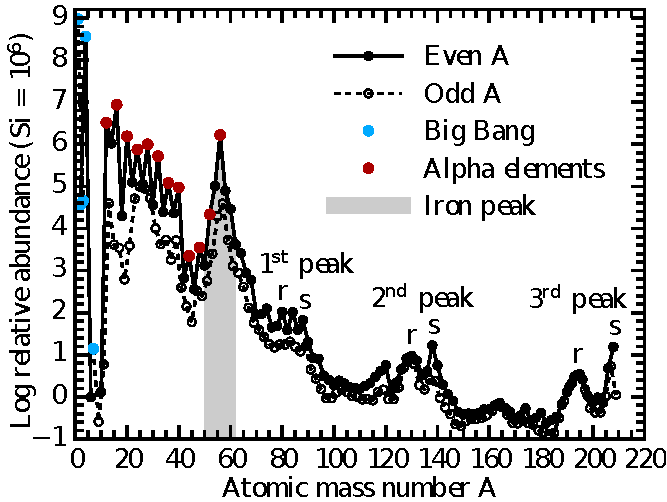
\includegraphics[width=0.49\textwidth]{Fig_1_1_Lip.pdf}
    \caption{Observed abundances in our solar system as a function of mass number
        $A$. The lightest elements were created in the Big Bang and fusion in stars predominantly
        creates alpha elements. The iron peak is made in core-collapse and type
        Ia \acp{SN}. Elements beyond the iron peak are synthesized by the slow ($s$) and
        rapid ($r$) neutron capture processes. These processes produce three distinct double
        peaks. Abundance data from \citet{Lodders:2003}. (Adapted from \citet{Lippuner:2018phd})
    }
    \label{fig:nuc:fig11_lip}
\end{figure}

%\begin{sidenote}
%    \textcolor{red}{Figure with solar observed abundances, showing $r$-elements and $s$-elements}
%    The observed obundacnes as a function of atomic mass number $A$ are shown in figure Fig. (XXX). 
%(data from \cite{Lodders:2003}). The plot shows nuclei that are more bound (due to spin pairing of nucleons 
%\cite{Moller:1993ed}), \textit{i.e,} those with an even $A$ number, are more abundant. The lowest binding 
%energy of nuclei with odd number of neutrons and protons (but even $A$) are largely unstable or short-lived. 
%A few exceptions are \textit{e.g.,} $^{40}$K, $^{50}$V, $^{138}$La and $^{176}$Lu, 
%that have a half-life of at least $10^{9}$ years.
%\end{sidenote}

The dominant \nuc{} process, responsible for the production of elements, varies with the mass 
number $A$.
%
For instance, light elements $A<8$ were synthesized right after the Big Bang
in the process known as \ac{BBN}.
Nuclides before the iron peak, $12\leq A\leq 56$ come from stellar hydrostatic 
nuclear burning \citep[\eg][]{Rolfs:1988,Hasen:2004}.
Elements at the iron peak $50\leq A \leq 62$ produces mostly 
during the type Ia \acp{SN} or explosive silicon burning in \acp{CCSN} \citep[\eg]{Woosley:2002}. 
The conditions at these sights are such that the dense material at the \ac{NSE}\footnote{
    At \ac{NSE} three parameters describe the composition: 
    density, temperature and electron fraction $Y_e = n_p/(n_p + n_e)$, 
    where $n_e$ and $n_p$ are the (total) number density of electrons and protons 
    respectively \citep{Seitenzahl:2009}. 
    The composition at \ac{NSE} favors more tightly bound nuclides,
    as they are more difficult to photodissociate.
}, 
expands and cools down, enriching the \ac{ISM} with heavy elements \citep{Iwamoto:2000as}. 
%
%Most of the material beyond iron peak are produced via neutron capture processes 
%\citep{Burbidge:1957}.
Nuclides with $A\geq 56$ cannot be synthesized via standard cycles due to their 
strong Coulomb barriers. 
Thus, processes that do not involve charged particles become dominant. 
These are the neutron capture processes \citep{Burbidge:1957}.


%% -------------------------------------------------------
%%                   Nucleosynthesis Cites
%% -------------------------------------------------------

%\subsection{Nucleosynthesis up to the iron peak}
%
%
%\subsubsection{Big Bang nucleosynthesis}
%
%Light elements in the Universe, like hydrogen ($\sim 75\%$ by mass) and helium 
%($\sim 25\%$ by mass) alongside trace amounts of $^{3}$He and $^{7}$Li were created 
%during the \ac{BBN} (see \eg, \citet{Tytler:2000qf} and references therein). 
%And while only a small number of nuclides were involved in \ac{BBN}, 
%there are large discrepancies between \ac{BBN} models and observations. 
%For instance, the "lithium problem" \citep{Coc:2013eha}, which origin is not well 
%understood \citep{Fields:2011zzb}.
%
%
%\subsubsection{Low-mass stellar burning}
%
%In order to fuse massive nuclides and overcome the strong Coulomb barrier, high temperatures, 
%($\geq 10^6$ K) are required. Thus production of heavy elements from hydrogen and helium 
%is possible only in special environments, in particular, in the interior of stars 
%\citep{Bethe:1939}. 
%For the most of their lives stars burn hydrogen into helium. The process releases the 
%binding energy and maintains the hydrostatic stability of a star. After the hydrogen is 
%exhausted in the core, a core (atmosphere) contracts (expands), heats up (cools), and the 
%shell hydrogen burning is initiated, slowly depositing ashes, \eg, helium, into the inert core. 
%The star's subsequent evolution depends primarily on its mass. If the mass of a star 
%$M>0.5M_{\odot}$, at some point the helium in the core starts to fuse into $^{12}$C and 
%$^{16}$O and small amounts of $^{24}$Mg, $^{28}$Si. These elements are called 
%\textit{alpha elements} \citep{Rolfs:1988,Hasen:2004}. 
%The end of the core helium burning phase leads to another core contraction phase. 
%A star of a mass $\sim 8M_{\odot}$ would be able to ignite carbon and oxygen producing 
%heavier elements afterwards. A less massive star looses its outer layers and becomes a 
%slowly cooling degenerate core, a white dwarf.
%
%
%\subsubsection{nuclear burning is massive stars}
%
%For a star that has $M\geq 8M_{\odot}$, a sequence of burning stages follows, each of 
%which leads to the exhaustion of a respective fuel, contraction of the core and rise of 
%its temperature \citep{Woosley:2002}. Carbon burning leads to the production of 
%$^{20}$Ne, $^{23}$Na and free protons that contribute to the synthesis of non-alpha elements. 
%As temperature increases, the photodisintegration of $^{20}$Ne becomes possible and a small 
%amount of $^{24}$Mg is formed. Next, the oxygen burning occurs producing $^{28}$Si $^{31}$P, 
%and $^{28}$Si and $^{32}$S, that become dominant nuclides in the core by the end of oxygen burning \citep{Rolfs:1988}.
%
%The subsequent silicon burning proceeds at $T\sim3.5\times10^9$K through photodissociation 
%of some of the $^{28}$Si and a sequence of alpha particle captures, "alpha ladder", on the 
%remaining $^{28}$Si to form $^{32}$S, $^{36}$Ar, $^{40}$Ca, $^{44}$Ti, $^{48}$Cr, $^{52}$Fe 
%and $^{56}$Ni. This process lasts around a day \citep{Rolfs:1988,Hasen:2004}. Due to high 
%temperatures present at silicon burning, nuclides with $A\in[28, 62]$ fall into quasi-equilibrium, 
%meaning that these nuclides (with exception of $^{12}$C, $^{16}$O $^{20}$Ne and $^{24}$Mg), 
%alpha particles and protons participating in reactions, are in equilibrium with each other. 
%
%At $A=56$ the binding energy per nucleon appears reaches its maximum and the silicon burning 
%cannot produce heavier nuclides with the release of energy. As the fraction of $^{56}$Ni in the 
%core of a star increases, the support that nuclear burning has provided against gravitational 
%contraction falls. Meanwhile the mass of the degenerate core still increases as burning proceed in shells.
%However, when the electron degeneracy pressure can no longer counteract gravity, \ie, when mass 
%of the core exceeds the effective Chandrasekhar mass\footnote{
%    The collapse however occur before the core reaches Chandrasekhar mass, and the pressure 
%    support that rests on the availability of free electrons drops when electrons capture on 
%    the nuclides becomes possible. To account for this, the effective Chandrasekhar mass was 
%    introduced.
%}, 
%the core collapses leading to a \ac{CCSN} \citep{Woosley:2002}.
%Thus, the origin of more abundant alpha elements in the Universe is stellar fusion.
%
%
%\subsubsection{Iron Peak}
%
%At temperatures higher then $T\sim 5\times10^{9}$K nuclear \ac{NSE} establishes. This is a 
%balance between the fusion reactions forming a ($N,Z$) nuclide from $N$ neutrons and $Z$ 
%protons and photodissociation reactions, splitting it back. 
%At \ac{NSE} three parameters describe the composition: density, temperature and 
%electron fraction $Y_e = n_p/(n_p + n_e)$, where $n_e$ and $n_p$ are the (total) 
%number density of electrons and protons respectively \citep{Seitenzahl:2009}. 
%%
%The composition at \ac{NSE} favors more tightly bound nuclides, as they are more difficult 
%to photodissociate. Thus, if the conditions allow, \ie, temperature, density and electron 
%fraction of the mater, ($Y_e \sim 0.46$, an electron fraction of iron), nuclides at $A\sim56$, 
%\ie, iron peak elements, dominate \citep{Seitenzahl:2009}. 
%%
%For example, \ac{NSE} establishes during the type Ia \acp{SN}, when a thermonuclear 
%explosion of a white dwarf allows for sufficiently high temperatures and densities. 
%After the explosion, newly synthesized elements of the iron peak cools, and being stable, 
%remain in the expanding medium \citep{Iwamoto:2000as}.
%
%
%\subsection{Nucleosynthesis beyond the iron peak}
%
%Nuclides with $A\geq 56$ cannot be synthesized via standard cycles due to their strong Coulomb 
%barriers. Thus, processes that do not involve charged particles become dominant. 
%These are the neutron capture processes.
%%
As nuclides absorb neutrons and grow larger, their binding energy, $Q_n$, decreases. This process 
is stopped when $Q_n\sim1$~MeV and energetic photons start to knock out neutrons from a nucleus. 
This process is called photodisintegration and a location in the parameter space where it occurs, 
(that in turn dependents on temperature and density), is called the 
%% [IMPORTANT]
neutron drip line 
%% ---
\citep{Rolfs:1988}.

Nuclides produced via neutron capture are generally unstable to $\beta$-decay, with a timescale, 
$\tau_{\beta}$, that can be larger or smaller than a neutron capture timescale, $\tau_n$. 
In case when $\tau_{\beta}\ll\tau_n$, \ie, when a $\beta$-decay occurs faster then the next 
neutron capture, the process is called \textit{slow} or \sproc{}. 
Thus, by definition, the \sproc{} moves along the valley of stability\footnote{
    a region of stable nuclides in the nuclides chart -- a chart in terms of number of neutrons $n_n$ 
    and number of protons $n_p$.
}, departing no further than by a few nuclides away.
On the other hand, if $\tau_{\beta}\gg\tau_n$, \ie, when a neutron capture occurs much faster then 
a $\beta$-decay, the process is called \textit{rapid} or \rproc{}. This \nuc{} generates nuclides 
near (but not crossing) the neutron drip line (See Fig.~\ref{fig:nuc:fig16_lip}) \citep{Rolfs:1988}. 

\begin{figure}[t]
    \centering
    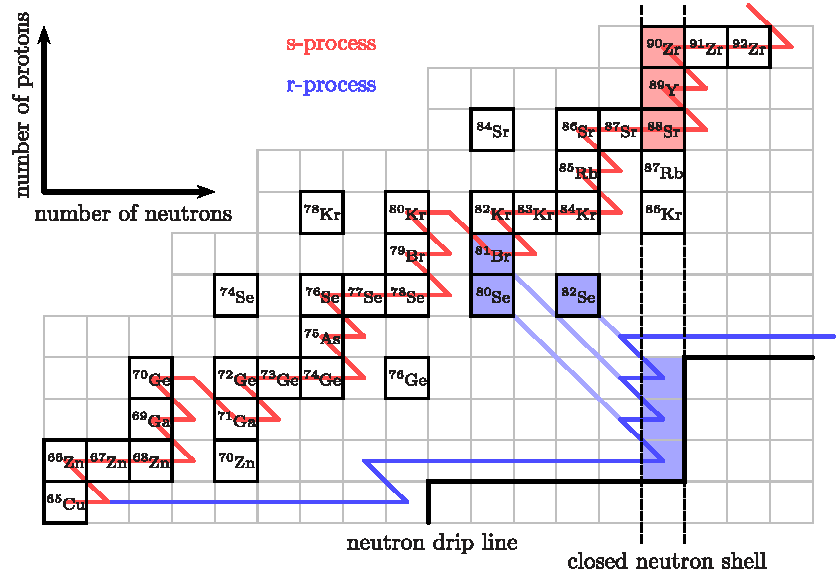
\includegraphics[width=0.60\textwidth]{Fig_1_6_Lip.pdf}
    \caption{Schematic representation of the $s$- and $r$-process on a section of the
        chart of nuclides. The s-process (red) proceeds along the valley of stability and the
        r-process (blue) along the neutron drip line. At the closed neutron shell N = 50, the
        neutron capture cross section drops by several orders of magnitude, which leads to a
        pile up of material there that produces the double-peak features
        (Adapted from \citet{Lippuner:2018phd})
    }
    \label{fig:nuc:fig16_lip}
\end{figure}
%
%% --- IMPORTANT --- ORIGIN OF THE PEAKS IN r-PROCESS
Notably, the trajectory of $r$-process is interrupted when the neutrons within a nuclide can arrange 
themselves in a closed shell. Such configurations are energetically very favorable and thus the cross 
section for a subsequent neutron capture reduces. Only after several $\beta$-decays does the 
$r$-process continue. Thus, nuclides located at points where neutron drip line and closed neutron 
shell overlap is more abundant. These unstable nuclides will decay back to the valley of stability 
and some of the neutrons within them turn to protons, reducing the total mass of them. The indication 
of this "overproduction" are the peaks in the abundance patterns at a mass, $A$, slightly lower then 
the one corresponding to a closed shell nuclide (see Fig.~\ref{fig:nuc:fig11_lip}).


%%% --- important
A similar "overproduction" of nuclides with a closed neutron shell occurs when an $s$-process 
is considered. However, in that case it is caused by the cross section of these nuclides being 
$1-2$ order of magnitude smaller then of neighboring ones \citep{Rolfs:1988}. Thus, in the case of 
\sproc{}, the peaks in abundance pattern will be at $A$, corresponding to the closed shell exactly, 
and thus located at larger $A$ than that of the \rproc{}. Closed shell nuclides are located at 
$N=50,\: 82, \: 126$ and thus corresponding abundance peaks for $s$-process are at 
$A=88, \: 138, \: 208$ and at $A=80,\:130,\:194$ for $r$-process (see \eg, \citet{Arnould:2007gh}) 
(See peak structure in Fig.~\ref{fig:nuc:fig11_lip}).

%% --- Motivation MP stars --- THE GENERIC SOLAR ABUNDANCES
It was found, that the solar \rproc{} abundance pattern is consistent, and can be found anywhere in the 
Universe. In particular, in stars that were formed very early on a galactic evolution timescale, the 
\ac{MP} halo stars, one would expect to observe less \sproc{} and \rproc{} elements as there might have 
been not enough time for the enrichment to take place. However recent studies showed that the solar 
\rproc{} abundances are present in these stars as well \citep{Sneden:2008,Roederer:2010}, 
see also Fig.~$8$ in \citet{Sneden:2009}. Thus, modeling the \rproc{} \nuc{} it is expected to 
reproduce the solar abundances.

%%% -- can be deleted
%It is important to note that in addition to \sproc{} and \rproc{}, a possible $i$-process, (intermediate) 
%is widely discussed. The process operates further from the valley of stability than \sproc{}, but not 
%reaching neutron drip line \citep{Cowan:1977,Bertolli:2013gka}. Slow and intermediate neutron capture 
%processes operate within the low-mass \ac{AGB} stars with mass $M\in[1.5,3]M_{\odot}$ and more massive stars,
%that enrich the interstellar medium with heavy elements via strong winds 
%\citep[\eg][]{Peters:1968,Couch:1974,Kaeppeler:1994K,Woosley:2002,Straniero:2005hc,Herwig:2011}. 
%The possible cites for the \rproc{} we discuss in the following subsections.


\subsubsection{Possible $r$-process sites}

Study of possible cites of \rproc{} is a wide and rapidly developing field. The general requirement 
for \rproc{} is a low electron fraction, or, in other words, neutron-rich conditions. These can be 
found in a various places for certain models of Big Bang, that include inhomogeneities, 
\ac{BNS} and \ac{NSBH} mergers and \ac{SN} ejecta (see \citet{Mathews:1990} and references therein). 
%
Spectral studies of \ac{MP} stars (formed early in the galactic history), combined with models of 
galactic chemical evolution sheds light on possible dominant cite of \rproc{} material. 
\textcolor{red}{add more sources/models}. 
It is now believed that certain types of \acp{SN} and \ac{BNS} mergers are the most likely 
sources on \rproc{} material \citep{Mathews:1990,Thielemann:2011} \textcolor{red}{add more sources}


%\subsubsection*{\acp{CCSN}}

Collapse of a massive star produces a hot neutron core, that undergoes deleptonization, releasing 
$\sim10^{53}$~erg of binding energy in form of strong neutrino flux. These neutrinos, irradiating 
dense medium around the core, can produce a \nwind{} \citep{Qian:1996xt}, that was suggested to be 
a promising cite for \rproc{} \citep{Woosley:2002,Wanajo:2006mq}. Later, it was shown however, that 
the electron fraction in the wind would be too high for a full \rproc{}, and only "light" heavy 
nuclide up to $A\sim130$ can be synthesized 
\citep{Qian:1996xt,Thompson:2001ys,Fischer:2010,Roberts:2010,MartinezPinedo:2012rb,Wanajo:2013} 
\textcolor{red}{add Perego:2017} 
%
It is important to note, in the proton-rich \nwind{} nuclides with $A\sim 100$ can be produces 
via so-called $\nu p$-process. The process relies on a creation of a free neutron from proton by 
an antineutrino capture. These free neutrons can then be captured by a seed nuclide, $^{64}$Ge seed 
nuclide and thus nuclides heavier then $^{64}$Ge can be created
\citep{Frohlich:2006,Pruet:2005qd,Wanajo:2010mc,Arcones:2012}
%
A full \rproc{} can be achieved in so-called magnetorotationally driven \acp{CCSN}. This is a rare 
type of \acp{CCSN}, where a core of the progenitor is rotating rapidly and is strongly magnetized. 
Induced by a magnetorotational processes \eg, magnetorotational instability, collapse is accompanied by a
formation of a collimated bipolar jet 
\citep{Wheeler:2000,Akiyama:2003,Burrows:2007yx,Mosta:2014jaa,Mosta:2015} \textcolor{red}{add Siegel2019?.}.
Materiel in these jets is predicted to be sufficiently neutron rich to allow for a full \rproc{} 
nucleosynthesis \citep{Winteler:2012,Nishimura:2015nca}. The rarity of this type of \acp{SN}, 
however, might not allow it to be the dominant source or $r$-process material \citep{Nishimura:2015nca} 
(\red{See however Seigal:PAPER}). 


%\subsubsection{Compact object mergers}
\red{TO BE REWRITTEN -- REPETITION OF PREVIOUS CHAPTERS}

%% --- MIGHT NEED TO BE SHORTENED A LOT!  OR MOVED TO INTRODUCTION!
Mergers of two \acp{NS} or a \ac{NS} and a \ac{BH} are regarded as one of the main cites 
of \rproc{} material \red{list of refs}. Compact objects, formed in a binary evolution of massive stars, 
orbit each other for gigayears, before slow loss of energy from the system due to \acp{GW} 
reduces their orbit and they merge \citep[\eg][]{Hulse:1975,Lattimer:2004sa,Price:2006fi}. 
%
%The late inspiral and merger of \ac{BNS} or a \ac{NSBH} have been studied extensively via smooth particle 
%simulations \red{[REFS]} \ac{HD} simulations \red{[REFS]} and \ac{NR} simulations with simplified gravity \red{[REFS]} 
%or full \ac{GR} \red{[REFS]}. The composition of a \acp{NS} in these simulations have been modeled with 
%simplified polytropic \red{[REFS]} or piece-wise polytropic \red{[REFS]} or microphsyical \acp{EOS} \red{[REFS]}. 
%The physical setup of these simulations have also evolved to eventually include effects of
%neutrino radiation transport \red{[REFS]} and magnetic fields \red{[REFS]}. 

%These studies have shown that shortly before and during the merger, the neutron star(s) undergo(s) a tidal 
%deformation and disruption. Streams of neutron-reach matter are then ejected into the circombinary 
%with enough energy to be not graviationally bound to the system \citep{Price:2006fi,Foucart:2014nda,Sekiguchi:2015dma,Kyutoku:2015gda,Radice:2016dwd}. 

%% For details on the ejecta from \ac{BNS} mergers see Chapter \ref{ch:BNS_results}.
%% In addition, in case of a \ac{BNS}, when \acp{NS} collide, material at the collision interface, heated by shocks, 
%% gets 'squeezed' and launched in the directions perpendicular to the plane of the binary \cite{Bauswein:2013,Hotokezaka:2013b} \red{[REFS]}. 
%% Generally, these tow components, tidal and shocked, constitute the \textit{dynamical ejecta}. Where the term 
%% ejecta referrers to the material that has enough energy to leave the system. 
%% The properties of the dynamical ejecta from BNS have a broad distribution, especailly in terms of mass and ejectron fraction 
%% [\red{[REFS]} \& myFitPaper], where the former lies in range $(10^{-4},10^{-2})M_{\odot}$ and the latter $(0.05,0.45)$. 
%% We discuss dynamical ejecta properties of BNS in more details in section \red{sec:results:dyn\_ej:prop} and nucleosynthesis 
%% in it in \red{sec:results:dyn\_ej:nucleo}. In case of NSBH the ejecta mass was shown be larger, reaching $0.1M_{\odot}$ with 
%% low electron fraction, $\leq0.2$ but it requires that masses of BH and NS are comparable and BH is rapidly spinning 
%% \cite{Foucart:2014nda}\red{[REFS]}. If the BH is much more massive then NS, the latter would be 'swallowed' with no ejecta \red{[REFS]}.
%% After the merger, there are expected to be additional ejecta. For general postmerger configuration consists of a remnant, massive neutron 
%% star (MNS) or a black hole sorrounded by a disk (torus) of bounded matter. In the first case,  a strong neutrino flux from cooling MNS and 
%% disk can drive an outflow in the direction, perpendicular to the plane of the binary, the so-called \nwind{} 
%% (see Figure 1 from \cite{Perego:2014fma}) \red{[REFS],Jujibayashi+20}. This ejecta is expected to occure on a timescales of 
%% $\sim100$ms postmerger, be not very neutron rich $Y_e\sim(0.2-0.45)$ due to neutrino irradiation and have a mass of 
%% $(10^{-4}-10^{-3})M_{\odot}$ \red{[REFS]}. 
%% The massive nutron star born in a merger exhibit dynamical oscillations \red{[REFS]}. The $m=1$ mode, so-called 
%% "one-armed spiral instability" especially can persisit on a $\sim100$ms powtmerger timescale and become a dominant mode 
%% \red{[REFS], MainPaper}. This oscillations can inject energy within the disk, where via angular momentum transport it leads 
%% to an outer part of the disk to become unbound. This ejecta, the \textit{\swind{}} was shown to occur in all cases where the MNS is present. 
%% It has high electron fraction and its mass depends on a lifetime of the remnant, and for a $\sim100$ms it can amount to a few 
%% $\times\sim10^{-2}M_{\odot}$ \red{[Letter, MainPaper]}. We discuss the mechanism that drives the \swind{} in the section 
%% \red{sec:results:swind:mechanism} and the ejecta properties in \red{sec:results:swind:prop} and corresponding 
%% nucleosynthesis in \red{sec:results:swind:nucleo}.
%% On a longer timescales, the viscous processes and alpha recombination in the disk, surrounding MNS or a BH are expected 
%% to unbind additional material. This is so-called \textit{secular ejecta}. It is expected to be massive and neutron rich. 
%% However, due to long timescales involved, it is very difficult model \red{[REFS]}.

\ac{BNS} and \ac{NSBH} mergers eject neutron rich material (see chapter~\ref{ch:bns_sims}) 
in which \rproc{} can take place, producing nuclides beyond $A=300$. Over-saturated with neutrons, nuclei 
are unsubtle to fission, and decay shortly after being formed. The decay products, before they reach the 
valley of stability, capture again free neutrons and grow up to $A=300$ and the cycle repeats. 
%% -- important 
This is so-called fission cycle. \red{might be better to remove it from here and discuss later}
%\subsubsection{Fission cycling}
%Fission cycling is a process where freshly synthesized via strong \rproc{} heavy nuclides 
%with $A\sim 300$ undergo fission just to become seed nuclides for a similar \rproc{} 
%leading to an $A\sim 300$ nuclide. This process eliminates the dependency of the final 
%abundances on the initial conditions and it also limits the maximum nuclide mass 
%that ca be achieved. 
%%
%The number of fission cycles can be estimated via a ration of the seed nuclides at time 
%zero and the number of seeds at the time when there are no more free neutrons available. 
%This is motivated by the fact that neutron capture itself does not create new seeds, only
%increases the mass of them, while fission, splitting heavy nuclide in two, generates 
%additional seeds. 
%%
%The number of fission cycles is tight to how much lanthanides and actinides are produced. 
%In particular, as fission cycling limits the maximum mass of the nuclide that can be created, 
%the fraction of lanthanides, actinides as well as heating $\varepsilon$ are insensitive 
%to the initial $Y_e$. The number of cycles is thus tight to the initial $Y_e$. The lower it is,
%the more free neutrons available and thus more cycles would occur. After the fission cycling
%stops the $r$-process maximum mass drops to $A\sim 250$. Thus the amount of actinides drops as
%only the lightest of them can be produced that do not fission immediately. 
%% --- 
It is maintained as long as there are free neutrons. After, the nuclides decay to the valley of 
stability for the last time, forming the remarkably robust abundance pattern, independent of the 
number of cycles \citep{Korobkin:2012uy,Bauswein:2013yna,Mendoza-Temis:2014mja}, 
(see also Figure 4 in \citet{Korobkin:2012uy}).
%
Numerical models have shown that the final \rproc{} abundances in the \ac{BNS} and \ac{NSBH} 
mergers ejecta are robust and reproduce the solar ones robustly 
\citep{Freiburghaus:1999,Goriely:2011vg,Goriely:2015fqa,Wanajo:2014wha,Just:2014fka,Radice:2016dwd}\red{[Refs]}. 
Recent observations of the one and only detected so far merger have confirmed that \ac{BNS} mergers do 
produce \rproc{} elements \red{[Refs] incl. Stroncium paper}.


\subsubsection{Galactic chemical evolution}

While there are several generally accepted cites for the \rproc{}, the main one is yet to be 
determined \citep[\eg][]{Qian:2000bh,Argast:2003he,Matteucci:2014}
%
%%% DELAY
For instance, the observed \rproc{} enrichment of \ac{MP} stars 
%if \ac{BNS} mergers are the main cite, than 
%the observed \rproc{} enrichment is difficult to explain as it 
requires very early source of \rproc{} material, when no mergers 
should have had happened yet, as the inspiral time ads a so-called \textit{time delay}.
This time delay before the compact binary binary formation and merger is 
$10^{6} - 10^{9}$ years \citep{DeDonder:2004cx,Dominik:2012kk}, and is highly uncertain and 
depends on a poorly understood common envelop evolution phase of the binary (progenitors)
\citep[\eg]{Dominik:2012kk}. 
%%%% SCATTER
Additionally, mergers of compact objects are rare events and thus expected to introduce 
a considerable scatter into the \rproc{} elements distribution in the Galaxy. 
However, observations show that the distribution is more uniform than expected \citep{Argast:2003he}.
%%%% CCSN as a contributor
Notably, recent population synthesis models have indicated that with a contribution from 
magnetorotationallydriven \acp{CCSN} the compact object mergers can account for the 
observed scatter of heavy elements \citep{Ishimaru:2015,Cescutti:2015,Wehmeyer:2015,VanDeVoort:2015}.
%
%%%% --------------------------------
%%%% IN MORE  DETAILS 
%%%% --------------------------------
%%%% Delay
%After the \ac{BBN}, the Universe consisting of hydrogen and helium, with traces of lithium, have expanded and cooled. 
%Under the influence of dark matter, the primordial gas fragmented, clumped and first stars, galaxies and galaxy 
%clusters have formed. During their lifetime the first stars (population III stars) converted light elements into 
%heavier ones and then ejected them into the \ac{ISM} during \ac{SN} events. Future populations of stars were born 
%of gas enriched with heavy elements, in particular, iron. Thus, the amount of elements heavier then hydrogen and 
%helium is stars (\ie, metallicity) increased with each stellar generation and there exists an age-metallicity relation 
%\citep{Matteucci:2012}. Important to note, that multiple dark matter sub-halos contributed to the formation of the 
%galaxy and there might not be a unique age-metallicity relation (see \eg, \citet{Ishimaru:2015} and references therein).
%%% Delay
%The enrichment of interstellar medium with heavy elements from stellar interior occurs immediately after stars die. 
%However, the \rproc{} elements, produced in \ac{BNS} (\ac{NSBH}) mergers can only enrich \ac{ISM} when compact objects 
%inspiral and merge which on average takes $(0.1-1)\times10^{9}$ years \citep{DeDonder:2004cx,Dominik:2012kk}. 
%The exact delay time is however highly uncertain and depends on a poorly understood common envelop evolution phase of the binary 
%(progenitors). And it was shown, that a small percentage of compact binaries might form with a time delay 
%before merger as small as $10^{6}$ years \citep{Dominik:2012kk}. 
%
%%% Study observations
%To study the chemical evolution of stars in the galaxy, the spectroscopic surveys\footnote{
%    And indicative quantity of metallicity measured in such iron-to-hydrogen ration, [Fe/H], that reads as a $\log_{10}$
%    of the abundance of a element $X$ to hydrogen, normalized to solar ration, \ie, in the sun for every X, [X/H]$= 0$. 
%    If a stars has [Fe/H]$=-2$, it is said that this star ahs a 100 times less iron compared to hydrogen then sun.
%} are conducted \citep{Edvardsson:1993,Suda:2008na}. 
%%% Scatter
%Mergers of compact objects are rare events and thus expected to introduce a considerable 
%scatter into the \rproc{} elements distribution in the Galaxy. However, observations show that the 
%distribution is more uniform than expected \citep{Argast:2003he}.
%%% Scatter
%However, recent population synthesis models have indicated that with a contribution from 
%magnetorotationallydriven \acp{CCSN} the compact object mergers can account for the observed 
%scatter of heavy elements \citep{Ishimaru:2015,Cescutti:2015,Wehmeyer:2015,VanDeVoort:2015}.
%
%% 244Pu
Comparison between the solar system and earth crust abundances of $^{244}$Pu have indicated that this 
nuclide might have been produced in rare events with high yield \citep{Wallner:2015}. This statement 
was confirmed via models of galactic mixing \citep{Hotokezaka:2015zea}, that also showed that there 
appears to be no degeneracy between rare high yields events (\ac{BNS}/\ac{NSBH}) 
and frequent low yield ones (\ie, \ac{CCSN}). Similar conclusion was draws from studying $^{244}Pu$ 
abundances in meteorites \citep{Tsujimoto:2017}.
%
%% UFDG
Study on \acp{UFG} also point towards a rare high yield events for \rproc{} nucleosynthesis. In particular, 
the \ac{UFG} Reticulum II was shown to have a solar \rproc{} abundances, while \ac{UFG} of similar type tend 
to have $2-3$ times less \rproc{} elements. This suggests that a rare high-yield event has modified 
Reticulum II chemical composition and high europium abundances indicate that it was a compact object merger 
\citep{Ji:2016}. 
%
%Thus it is still unclear whether observed degree of homogeneity in \rproc{} elements distribution in the galaxy and 
%\rproc{} elements enrichment of very \ac{MP} stars can be explained by compact object mergers only. 
%% Scatter

\red{Mention Actinide abundaces problem.}


%% =======================================================
%%
%%                   K I L O N O V A
%%
%% =======================================================

\subsection{Kilonova}

Nuclides, synthesized in \rproc{} are very neutron rich and unstable. After the last 
fission cycle, they decay to the valley of stability (see chapter~\ref{ch:nucleo}). 
%
%This process takes from hours to days and released energy 
%can power an \ac{EM} transient, called \ac{kN} or Macronova  
%\citep[\eg][]{Li:1998bw,Kulkarni:2005jw,Metzger:2010,Roberts:2011,Metzger:2016pju,Wollaeger:2017ahm}
%
%
%During the \ac{BNS} mergers, the neutron-rich material is ejected 
%(see Chapter \ref{ch:bns_sims} for details). The conditions of the eject are such that they allow 
%for the \rproc{}, that produces heavy elements far from the valley of stability (see Chapter 
%\ref{ch:nucleo} for details) 
Li et al., \citep{Li:1998bw} suggested that an \ac{EM} transient can be powered by the radioactive 
decay of the material enriched with \rproc{} elements, ejected in \ac{BNS} or \ac{NSBH} mergers. 
They also showed that contrary to the normal \acp{SN}, the ejecta would quickly become transparent 
to its own emission, peaking on a timescale of around a few days. The main difficulty in this 
pioneering work was the lack of a \ac{nuc} model to model to estimate the radioactive heating of the 
ejecta. 
%
The understanding of \ac{kN} has significantly improved since then
\citep[\eg][]{Kulkarni:2005jw,Metzger:2010,Roberts:2011,Metzger:2016pju,Wollaeger:2017ahm}
%
but the only unambiguous detection of \ac{kN} so far, was the thermal transient, \AT{}, 
\citep{Coulter:2017wya,Chornock:2017sdf,Nicholl:2017ahq,Cowperthwaite:2017dyu,Tanvir:2017pws,Tanaka:2017qxj}
that was observed after the \ac{GW} trigger, \GW{}, 
\citep{TheLIGOScientific:2017qsa,Abbott:2018wiz,LIGOScientific:2018mvr}.
%
This observation provided evidences that the ejection of neutron-rich matter from compact 
binary mergers is one of the primary site for \rproc{} nucleosynthesis 
%\citep{Lattimer:1974slx,Li:1998bw,Kulkarni:2005jw,Rosswog:2005su,Metzger:2010,Roberts:2011,Kasen:2013xka}.
\citep{Arcavi:2017xiz,Coulter:2017wya,Drout:2017ijr,Evans:2017mmy,Hallinan:2017woc,Kasliwal:2017ngb,
    Nicholl:2017ahq,Smartt:2017fuw,Soares-santos:2017lru,Tanvir:2017pws,
    Troja:2017nqp,Mooley:2018dlz,Ruan:2017bha,Lyman:2018qjg}. 
%The \ac{kN} is the \ac{EM} \ac{UV}/optical/\ac{NIR} transient, powered by the 
%radioactive decay of the elements synthesized via \rproc{} in expanding ejecta.
%
The peak in \ac{NIR} band of \AT{} occurred several days after the merger \citep{Chornock:2017sdf}.
It is generally consistent with emission from the high opacity material, with a sizable 
fraction of lanthanides \citep{Kasen:2013xka}
%
The peak in \ac{UV}/optical band, however, occurred in less than one day after the merger 
\citep{Nicholl:2017ahq}. This requires the opacity of the material to be sufficiently low, 
suggesting that only partial \rproc{} \nuc{} took place in the corresponding ejecta 
\citep{Martin:2015hxa}.
%
These observations that material with distinctly different properties contributed to the emission.
%
% [RED]
%\ac{kN} has a complex observational signature due to different ejecta components with various 
%compositions contribution to it. 
In particular, it was shown that if produced, 
lanthanides $(58\leq Z \leq71)$ and actinides $(90\leq Z \leq 103)$ with their open $f$-shell 
and hence a plethora of absorption lines, increase opacity of emitting region by a factor of $10$. 
%
These elements are produced only if electron fraction of the ejecta was sufficiently low, 
$Y_e\leq 0.25$ \citep{Lippuner:2015gwa}, present for example in a tidal component of \ac{DE}. 
High opacity would imply that a transient is dim $(\sim10^{40})$ erg s$^{-1}$ and peak around a 
weak after merger in the red/infrared band \citep{Barnes:2013wka,Grossman:2013lqa,Lippuner:2015gwa}. 
%
% [BLUE]
If the ejecta electron fraction is high, $Y_e \geq 0.25$, weak \rproc{} would produce a small amount 
of lanthanides and the opacity of the emitting region would thus be lower. The kilonova signal originating 
from such ejecta would be bright and peak on a timescale of a few days in blue band 
\citep{Kasen:2014toa,Martin:2015hxa}. 
%
%
Indeed, both and red components were observed in the case of \AT{}, that confirmed the general 
picture \citep[\eg][]{Villar:2017wcc}. However, estimated mass of the ejecta required to explain 
the red component is larger then what is predicted by numerical relativity simulations \red{refs}. 
It is believed that the most contribution to this component comes from the low $Y_e$, slow but 
massive outflow from the degenrate disk on a secular timescale \red{refs}.
%
Semi-analytic two-components (red and blue) spherical \ac{kN} models to the \AT{} observations 
provided estimates for the ejecta properties for these two components. 
%
Specifically, for the langhinide poor (rich) \ie, blue (red) components, the required mass is 
$2.5\times10^{-2}M_{\odot}$ ($5.0\times10^{-2}M_{\odot}$) and velocity $0.27$c ($0.15$c)
\citep{Cowperthwaite:2017dyu,Villar:2017wcc}. 
See however \citep{Waxman:2017sqv} for an alternative interpretation.
See also \citep{Siegel:2019mlp} for the compiled data on the \ac{kN} models.
%
Similar estimates are obtained with $1$D radiation transport \ac{kN} models
\citep{Tanvir:2017pws,Tanaka:2017qxj}.
%
%A very high energy emission from the non-thermalized radiation is weak and can be 
%detected only for a sufficiently close event \cite{Hotokezaka:2015cma}.
% 
Notably, prior to \AT{}, there were other candidates based on the detection of \ac{SGRB}, 
with infrared excess \eg, 
GRB130603B, \citep{Berger:2013wna,Tanvir:2013pia}, 
GRB060614 \citep{Jin:2015txa,Yang:2015pha}, 
GRB050709 \citep{Jin:2016pnm}.
GRB200522A \citep{WRONG}  Bruni:2021ilp
However the exact nature of the observed signals were not well constrained. 
%
The search for \ac{EM} counterparts to mergers continues, involving observatories around the world 
\citep{Law:2009,Singer:2014qca,Bellm:2014,Kasliwal:2016uhu}.
%


%% =======================================================
%%
%%                   G R B  A F T E R G L O W
%%
%% =======================================================


\subsection{$\gamma$-ray bursts and kilonova afterglows}

\acp{GRB} are irregular pulses of gamma-ray radiation with broken power-law 
(non-thermal) spectrum, peaking at KeV-MeV \citep{Band:1993,Kouveliotou:1993,Meegan:1992xg}.
%
With respect to the duration, \ac{GRB} are split into two categories: \ac{SGRB}, 
that last ${\leq}2$~s and long \ac{GRB} that last ${\gtrsim}2$~s. The latter are the 
result of the collapse of massive ${\geq}15M_{\odot}$ stars, while the former, at 
least in part, is attributed to mergers of compact objects. Only very recently it 
was directly confirmed with the detection of \ac{SGRB} \GRB{} that accompanied 
the \ac{GW} event \GW{} \citep{TheLIGOScientific:2017qsa}. However, the exact physical 
origin of different duration \ac{GRB} is not fully understood.
%
Indications that long \ac{GRB} are associated with core-collapse supernovae, \acp{SN}, 
are two fold. These \acp{GRB} are typically observed in star-forming regions of their 
host galaxies \citep[\eg][]{Bloom:2000pq,Bloom:2002hc,Fruchter:2006py,Christensen:2004yx,CastroCeron:2006jh} 
and several \acp{GRB} are spectroscopically associated with Type Ic \acp{SN}, albeit 
these \acp{GRB} were significantly less bright and might not be typical \acp{GRB} 
\citep[\eg][]{Liang:2006ci,Bromberg:2011fm}. Additionally, the late time behaviour 
of some \acp{GRB} includes a \acp{SN}-like "bump" in the optical and spectral changes 
that might imply that underlying \acp{SN} flux becomes dominant over \acp{GRB} 
\citep[\eg][]{Bloom:1999,Woosley:2006fn}.
%
The \acp{GRB} are distant events, most of which were localized to outside the local 
group \citep[\eg][]{Mao:1992,Piran:1992,Fenimore:1993}. Particularly useful for distance 
estimation were the observations of \ac{GRB} afterglow, fading X-ray \& optical emission, 
that allow to estimate the redshift \citep[\eg][]{Costa:1997cg,Frontera:1997ae}.
%
Analysis of the multi-wavelength afterglow data for \acp{GRB} \citep[\eg][]{Panaitescu:2001bx} 
suggested the mechanism behind the afterglow emission is the synchrotron radiation from the 
external forward-shock, which forms when \ac{GRB}-ejecta sweeps-up the \ac{CBM} or \ac{ISM}
medium\footnote{
    The specific indications are the power law decay of the light curves, 
    $F_{\nu}\propto^{-1}$ and power-law spectrum $F_{\nu}\propto\nu^{-0.9\pm 0.5}$.
} 
\citep{Rees:1992ek,Paczynski:1993gz,Meszaros:1993ju,Meszaros:1996sv}.
%
The temporal behavior of many (but not all) \acp{GRB} shows a change, a steepening 
of the light-curve (to $F_{\nu}\propto t^{-2.2}$) at $\sim 1$~day after the burst. 
This is usually attributed to the 
%\gray{deceleration of the colimated GRB-outflow, jet, and decrease on the realtivisitc beaming. This in turn makes the edge of the jet visible to an observer.} 
finite angular extend of the \ac{GRB}-ejecta, jet \citep[\eg][]{Rhoads:1999wm,Sari:1999mr}. 
When jet decelerates and relativistic beaming decreases (and the jet edge becomes visible), 
the optical and X-ray lightcurves decay achromatically faster. This achromatic transition 
from slow to faster decay is called "jet-break".
%
%%% PROBLEMO -- jet-break is not a universal feature.
%Notably, this jet-break is not observed in all \acp{GRB} for the reason that is not fully 
%understood \citep[\eg][]{Fan:2006pj,Panaitescu:2006,Liang:2007ti,Sato:2006jg,Liang:2007rn,Curran:2007cp,Racusin:2008bx}
%%
%%% PROBLEMO -- GRB density seems uniform, but SSE models predict wind-like profile
%Models of the broadband emission of \acp{GRB} with jet-break showed that the 
%\ac{CBM}, is uniform with number density \red{$\sim 10^{-3}$} \citep{Panaitescu:2001bx}. 
%If \acp{GRB} produced in collapse of massive stars \citep{Woosley:1993,Paczynski:1997yg}, 
%this contradicts the expected density profile from stellar winds, \eg, $\rho\propto r^{-2}$ 
%\citep[\eg][]{Dai:1998iz,Chevalier:1999jy,Chevalier:1999mi,Ramirez-Ruiz:2001} 
%\red{this might be very outdated.}
%
%% sGRB
The origin of \acp{SGRB} was first connected with the elliptical galaxes, and with 
older stellar population 
\citep[\eg][]{Gehrels:2005qk,Fox:2005kv,Barthelmy:2005bx,Berger:2005dr,Panaitescu:2005er,Bloom:2005qx,Guetta:2005bb,Nakar:2007yr} 
and thus with \ac{BNS} mergers. A more direct evidence came with the \GRB{}
\citep{Savchenko:2017ffs,Alexander:2017aly,Troja:2017nqp,Monitor:2017mdv,Nynka:2018vup,Hajela:2019mjy}, 
detected by the space observatories Fermi \citep{TheFermi-LAT:2015kwa} and INTEGRAL \citep{Winkler:2011}.
%
Generally \acp{SGRB} show a complex time behavior of early afterglow X-ray emission, 
in particular a presence of a plateau ($F_{x}\propto t^{-1/2}$), after the initial sharp 
decrease ($F_{x}\propto t^{-3}$) which a standard forward shock model does not predict. 
This implies that early X-ray afterglow is shaped by a variety of physical processes 
\citep{Zhang:2005fa}.
%
The \GRB{} was dimmer then any other events of its class. 
Different interpretations for its dimness and slow rising flux were proposed: off-axis jet, 
cocoon or structured jet. Now it is commonly accepted that \GRB{} was a structured jet 
observed off-axis 
\citep[\eg][]{Fong:2017ekk,Troja:2017nqp,Margutti:2018xqd,Lamb:2017ych,Lamb:2018ohw,Ryan:2019fhz,Alexander:2018dcl,Mooley:2018dlz,Ghirlanda:2018uyx}.
The \GRB{} late emission, the afterglow, provided information on 
the energetics of the event and on the properties of the circumburst medium 
\citep[\eg][]{Hajela:2019mjy}. 

%%%% EARLY emission problem
%Two main questions stem from these observations: is the mechanism behind the prompt 
%$\gamma$-ray emission and early afterglow emission is the same (or do they originate from 
%the same outflow), and is the early X-ray radiation produced by the external shock (just a 
%blast wave takes long time to become self-similar) or does it originate from an internal 
%shock? An indication that the long-lived central engine activity might affect the 
%afterglow came from the observed sharp increase in X-ray flux (flares) on a 
%scale of minutes to hours after the end of the \ac{GRB}
%\citep{Burrows:2005ww,Chincarini:2007fp,Chincarini:2010,Margutti:2011}, 
%which could not be attributed to the inhomogeneities in the \ac{CBM}.
%%% PROBLEMO!
%Thus, the early X-ray behaviour of \acp{GRB} $t < 10^{4}$~s post-burst is not well 
%understood and seems to be in tension with standard afterglow forward shock emission model.

%\textcolor{red}{
%    One of the foremost unanswered questions about GRBs is the physical mechanism
%    by which prompt $\gamma$-rays the radiation that triggers detectors on board
%    GRB satellites are produced. Is the mechanism the popular internal shock
%    model 6 \cite{(Rees and Meszaros, 1994)}, the external shock model, or something
%    entirely different? Are $\gamma$-ray photons generated via the synchrotron process
%    or inverse-Compton process, or by a different mechanism? Answers to these
%    questions will help us address some of the most important unsolved problems
%    in GRBs  how is the explosion powered in these bursts? Does the relativistic
%    jet produced in these explosions consist of ordinary baryonic matter, electron positron
%    pairs, or is the energy primarily in magnetic fields?
%}

%Once again, while it is suggested that the high energy emission, after the propmt phase is produced 
%by the synchrotron process in the external forward shock, \citep{Kumar:2009,Ghisellini:2010}, 
%the mechanism behind the high and low energy $\gamma$-ray emission in the prompt phase remains unknown. 
%Possible mechanisms include: inverse Compton and synchrotron emission in internal and external shocks
%\citep[\eg][]{Rees:1992ek,Dermer:1998py,Lyutikov:2003ih,Zhang:2011} and 
%photospheric radiation with contribution from multiple \ac{IC} scatterings
%\citep[\eg][]{Thompson:1994zh,Ghisellini:1998jy,Meszaros:1999gb,Peer:2005qoc,Peer:2008udu,Giannios:2006jb,Ioka:2007qk,Asano:2009gi,Lazzati:2010,Beloborodov:2010,Toma:2011}.

%% from the Afterglow paper



%\subsection{kilonova afterglow}

In addition to the \ac{GRB} beamed emission, the non-thermal, more isotropic 
emission is expected from electrons accelerated in shocks formed between the 
(mildly) relativistic ejecta and the \ac{ISM} \citep{Nakar:2011cw}. This emission 
is expected to peak in radio band and continue on a time scale of tens of years 
after merger. Notably, all ejecta components will contribute to the emission, 
but depending on the ejecta velocities and kinetic energy, 
the brightness in different frequencies and timescales differs. 
%
Various ejecta components interact with each other and with \ac{ISM}. The latter, 
generates a long-lived blast wave. The shock, propagating upstream, amplifies 
(random) magnetic fields and accelerates electrons, that subsequently emit 
synchrotron radiation. This process in phenomenological similar to the for the 
\ac{GRB} afterglow and \ac{SN} early remnants. 
%
Numerical simulations of \ac{BNS} mergers showed the presence of mildly relativistic 
ejecta (See Sec.~\ref{sec:bns_sims:method:ejecta}). 
Several studies on the possible non-thermal electromagnetic emission of this ejecta 
have been carried out 
\citep[\eg][]{Piran:2012wd,Hotokezaka:2015eja,Hotokezaka:2018gmo,Radice:2018pdn}. 
Notably, the observed non-thermal emission from \GW{}, was first interpreted 
as the non-thermal emission from the ejecta \citep{Mooley:2017enz}.
This interpretation was however disproved by the emergence of jet break
%
%Specifically, a strong radio emission is expected from \ac{BNS} ejecta \citep{Piran:2012wd,Hotokezaka:2015eja}. 
The \ac{BNS} merger radio remnant is expected to peak on a time-scale 
of years after the merger and be visible over a similar timescale. Notably, this is 
assuming that the ejecta is expanding into the unshocked \ac{ISM}, as it was shown 
that if the \ac{ISM} is pre-shocked by the jetted outflow, and the \ac{ISM} density is 
reduced, the kilonova afterglow would be delayed. 
%
In \citet{Piran:2012wd}, the synthetic \ac{kN} afterglow \acp{LC} are calculated 
for a set of \ac{NR} \ac{BNS} merger simulation with properties typical to the 
Galactic binary population and \ac{ISM} density usually found in the Galactic disk, 
$\nism\sim1\ccm$. Authors showed that the from a binary of two $1.4\Msun$ \acp{NS}, 
the kilonova afterglow would peak $\sim10$~years after the merger if $\nism = 0.1\ccm$ 
and $\sim3$~years if $\nism = 1\ccm$ in radio bands, $\nu=1.4$~GGz and $\nu=150$~MGz. 
Notably, both values of the \ac{ISM} density are larger than what is inferred for \GW{}. 
Indeed, jet fitting models and dependent analysis of the diffuse emission suggest 
$\nism\in(10^{-4},10^{-2})$\gcm \citep{Hajela:2019mjy}.
%In \citet{Piran:2012wd} authors focus on the observational prospects of this afterglow 
%and compare it to other \ac{EM} emission expected for \ac{BNS}. 


%% =======================================================
%%
%%                   G W s
%%
%% =======================================================

%\section{Gravitational Waves}

%% =======================================================
%%
%%                   T H E O R E T I C A L  P I C 
%%
%% =======================================================

\section{Theoretical picture}

The properties and structure of matter at nuclear saturation density, 
$\rho_{\rm nuc}\approx2.7\times10^{14}\,$\gcm, are not well understood partially due to 
the complexity of the \ac{QCD} many-body problem and partially to to the 
inaccessibility of these densities in modern laboratories on Earth. Thus, the \ac{NS} 
\ac{EOS}, especially at densities near and above $\rho_{\rm nuc}$ remains rather uncertain.
So does the \ac{NS} mass-radius relation, calculated for a given \ac{EOS} via relativistic 
hydrostatic stellar-structure equations (also known as \ac{TOV} equations). 
Depending on the slope of the mass-radius relation, the \acp{EOS} are loosely divided into 
``stiff'' and ``soft''. Additionally, the stiff (soft) \acp{EOS} allow for higher (lower) 
values of the the maximum possible gravitational mass\footnote{
    We generally refer to the mass of a \ac{NS} star as its gravitational mass, which 
    is smaller with respect to the baryon mass by the amount of gravitational 
    binding energy. 
} for a non-rotating \ac{NS} (exceeding which a \ac{NS} collapses to a \ac{BH}).
For most microphysical \ac{EOS} 
the maximum mass falls in range $M_{\rm max}=1.5-2.5\,\Msun$ \cite{e.g. Lattimer & Prakash, 2000)}
This estimate is being continously updated as more and more massive puslars are being 
discovered \cite{e.g. Demorest et al., 2010} and \ac{MM} analysis is being advanced.
See Sec.~\ref{sec:nr_methods:eos} for more details.
%The maximum mass of a rigidly rotating \ac{NS} is even more complicated to asses 
%and requires solving equations of \ac{GR} in a certain approximation, and depends 
%sensibly on the 

Models of \ac{BNS} mergers were first envisioned by \cite{Lattimer & Schramm (1974, 1976)},
who also identified these events as possible sources of \rproc{} elements. 
More sophisticated modeling of the merger dynamics that does not rely on point-mass 
approximation or specific equilibrium assumptions became available when the computational 
resources sufficiently expanded \cite{see Faber, 2009; Duez, 2010, for recent reviews}.
In this section we briefly outline the current understanding of the \ac{BNS} mergers, 
that is overall based exclusively on the resuts of \ac{NR} simulations. In sections 
\ref{xxx} and \ref{yyy} we discuss the postmerger evoltuion. 
Due to high computational cost of these simulations, the \acp{NS} are usually 
initialized on a quasi-circular orbit, ${\sim}4-5$ orbits before merger. The evolution 
of the system after merger is computed for $\gtrless100\,$ms with the most advanced codes.


\subsubsection*{Binary neutron star mergers}

The first \ac{BNS} simulations were performed using Newtonian physics, a polytropic \ac{EOS} 
(see Sec.~\ref{sec:nr_methods:eos}}) and a separate scheme to account for the emission of \acp{GW} 
\cite{(e.g. Oohara & Nakamura, 1989; Shibata et al., 1992; Rasio & Shapiro, 1992)}.
As methods advanced and computational resources increased, the focus of merger simulations 
split. Certain groups focused on including more 'matter physics', \eg, microphsyical \ac{EOS}, 
approximate neutrino readiation transport, effects of magnetic fields and turbulence, while 
others proceeded with simplified \acp{EOS} but more sophisticated implementations of \ac{GR}, 
via post-Newtonian methods \cite{(e.g. Faber & Rasio, 2000)}, 
relativistic conformal-flatness approximation \cite{(e.g. Wilson et al., 1996; Oechslin et al., 2002; Faber et al., 2004)} or considering the fill-\ac{GR} \cite{e.g., Shibata & Uryu, 2000; Baiotti et al., 2008; Thierfelder et al., 201}. Recently, these simulations that adopt both, full \ac{GR}, microphsycial \ac{EOS},
advanced treatment of neutrinos and \ac{MHD} turbulence emerged \cite{ OUR SIMULATIONS \& Rezolla \& shibata}
The self-consistent implementation of magnetic fields into the simulations were implemented in 
alongside Newtonian physics by \cite{Price & Rosswog (2006)} full general relativity, 
\cite{e.g., in Anderson et al. (2008); Liu et al. (2008); Giacomazzo et al. (2009)}.

\begin{figure}[t]
    \centering
    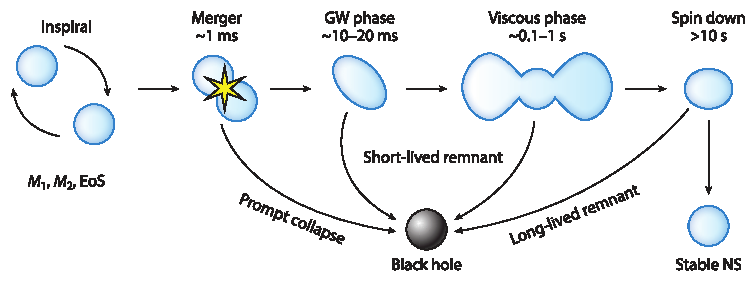
\includegraphics[width=0.60\textwidth]{Fig_3_Rad.pdf}
    \caption{
        Overview of the different phases in an NS merger and the relative timescales. 
        The inspiral ends with the merger, when the two stars start to fuse together. 
        The early \pmerg{} evolution is entirely driven by hydrodynamics and by \ac{GW} emission. 
        If the remnant does not collapse within ${\sim}10-20\,$ms, \ac{GW} losses
        subside and other physical processes become more important: 
        Angular momentum redistribution (which is due to turbulent viscosity) 
        and neutrino losses operate over a timescale of a tenth of a second to a few
        seconds. This is also the characteristic timescale for the evolution of the remnant disk. 
        If the remnant does not collapse over a timescale of a few seconds, then it will 
        spin down because of \ac{MHD} effects over a possibly much longer timescale 
        of several seconds to a few hours. 
        (Adapted from \citet{Radice:2020ddv})
    }
    \label{fig:intro:pic}
\end{figure}

The qualitative picture of the \ac{BNS} merger dynamics is depicted in Fig.~\ref{fig:intro:pic}. 
The main parameters that determine the evolutionary path are the total gravitational mass, 
$M_{\rm tot}$, \mr, $q$, and \ac{EOS}. The intrinsic angular momenta (also called spin) of \acp{NS} 
can be neglected to a certain extend as (i) astrophysical \acp{NS}, observed as pulsars, have 
spin lower than the orbital angular momentum of the system and (ii) the \acp{NS} internal 
viscosity is too low to allow for tidal locking make stars co-rotate \cite{(e.g. Bildsten & Cutler, 1992)}.

It is possible that the object formed after the merger has mass exceeding $M_{\rm max}$. 
The remnant might still avoid the fate of collapsing to a \ac{BH} immediately, if the differential 
rotation is strong enough to provide additional support against gravity. The mass threshold 
for that is rather uncertain but is estimated to be $M_{\rm crit,1}\sim1.3-1.7M_{\rm max}$ 
(e.g. Shibata et al., 2003; Shibata & Taniguchi, 2006). Such an object is commonly referred to as 
\ac{HMNS}. Its lifetime is determined by the rate at which it is loosing energy to, \eg, \acp{GW}
and the angular momentum is being redistributed, making it more compact. 
Another threshhold mass is the maxiumum mass that a rigidly rotating \ac{NS} can have, the 
$M_{\rm crit,2}$ and is $M_{\rm crit,2}{\lesssim}1.2M_{\rm max}$ \cite{Cook et al., 1994}. 
%If the newly formed remnant has mass lower than $M_{\rm crit,2}$, it can in principle survive 
%for 
If the newly formed remnant has mass exceeding $M_{\rm crit,2}$, it is expected to collapse to 
a \ac{BH} after the redistribution of the angular momentum. However, this scenario remains 
unconfirmed as it requires long-term, fully self-consistent investigation with expensive 
\ac{NR} simulations. In this thesis we attempt to constrain this evolutionary path.

After the merger, a remnant, be it a \ac{NS} or a \ac{BH} can be surrounded by a matter, that 
have a different rotation profile, lower density (compare to \ac{NS}) but still gravitationally 
bound to the central object. This matter is generally called disk or torus. Its mass and 
properties are crucial in determining the long-term evolution of the system and \pmerg{} 
outflows. However, they are not well understood on a quantitative level, as long-term 
self-consistent \ac{NR} simulations with advanced physics input that are required for their study 
are very computationally expensive. 
%In this thesis we attempt to advance our understanding of the disk by by means of our 
%own \ac{NR} simulations and via statistical analysis of all the data publicly available from 
%other groups.

%%%% <<< moved from BNS_merg_sims :: ejecta >>> 
When \acp{NS} collide and merger, matter is ejected through a number of 
different physical processes, gaining enough energy to become graviationally 
unbound (according to the criteria discussed in Sec.~\ref{sec:bns_sims:method:ejecta}). 
%\alpedit{The matter ejected on dynamical timescale of the system (${\sim}10$~ms) 
%is called the dynamical ejecta.}{
In particular, the matter ejected within a few dynamical timescales (\ie, ${\sim}10$~ms) 
after merger by tidal torques and hydrodynamics shocks driven by core bounces 
is called \ac{DE} \citep[\eg][]{Hotokezaka:2013b,Bauswein:2013yna,Radice:2016dwd,Radice:2018pdn}. 
%
% From AFTERGLOW paper
%
Several mechanisms contribute to the ejection, and depending on the 
binary parameters, their relative contribution differs.
%
For instance, shortly before and during the merger, the outer parts 
of the \acp{NS}, opposite to the collisional interface, are stripped 
away by the tidal torque and centrifugal forces. This is the tidal 
component of the \ac{DE}. It is more massive in binaries with 
larger \mr{} and is maximum in those that experience tidal disruption 
\citep[\eg][]{Radice:2018pdn,Bernuzzi:2020txg}.
%
Such ejecta is neutron rich, confined largely to the orbital plane and exhibits 
a crescent-like azimuthal structure \citep{Bernuzzi:2020txg}.
%
Overall, the tidal ejecta component is mostly equatorial and its 
velocity is related to the \acp{NS}' velocity at merger and 
and the system's escape velocity, and is $\sim0.2$~c.
%
When \acp{NS}' cores collide and bounce, shocks propagate outwards inducing 
matter ejection. Additionally, a small amount of material at the 
\acp{NS}' collisional interface is shock-heated and launched into the polar 
direction. This comprises the shocked component of the \ac{DE}.
%
It is more massive and faster if \acp{NS}' radii are smaller and they collide 
at higher velocities \citep[\eg][]{Radice:2018pdn}. 
%
Overall the dynamical ejecta has a broad distribution in terms of composition, 
velocity and mass, dependent on the parameters of the binary and \ac{NS} \ac{EOS}.
%% === ON THE FAST DYNAMICAL EJECTA IN PARTICULAR ===========

\red{Might add 'on a longer timescale other ejecta components are expected'}


\subsection{Accretion disks}

Accretion disks comprise the matter that is orbits the central object near rotational 
equilibrium and accretes onto the central object. Such phenomena can be found in a variety of 
incarnations and on a broad range of spatial scales in the Universe, \eg, around proto-stellar
object during the star formation, in X-ray binaries, when the matter from the massive 
companion star is being accreted onto a compact object, or in \ac{AGN}
\cite{see e.g. Pringle, 1981; Balbus & Hawley, 1998; Spruit, 2010a, for reviews}.
While being studied for a long time via a broad range of methods, the key physical mechanisms, 
that induce the accretion, \ie, the transport of angular momentum, is not well understood.
This problem becomes considerably more complex, when the central object is not axisymmetric 
and interact with the disk. 
One of the mechanisms responsible for the transport of angular momentum, is the torque between
differentially rotating fluid elements exerted by microscopic viscosity. However, it is 
orders of magnitudes weaker than what is required to explain the observed accretion rates 
\cite{e.g. Lust, 1952} 
%Additionally, an effecitve shear streses are generated in the flued
%that is sugjected to stochastic small-scale motions in the flow tih high Reynolds nuimbers.

\paragraph{The $\alpha$-viscosity approximation}

It is possible to describe the disk turbulence without known the exact mechanism responsible 
for it. Shakura \& Sunyaev (1973) \cite{Shakura & Sunyaev (1973)} proposed a method to 
parameterize the shear stress under the assumption that the disk flow is quasi-laminar. 
This is so-called ``turbulent kinematic $\alpha$-viscosity'' model, that can be derived 
from the dimensional analysis. For the characteristic quantities of the local disk medium, 
the sound speed $c_s$ and the Keplerian\footnote{
    By Keplerian we imply a stationary orbit, where the gravitaional attraction is balanced 
    by the centrifugal force exactly.
} angular velocity $\Omega_K$, the $\alpha$-viscocity more reads 
%
\begin{equation}
    \nu_{\rm vis} = \alpha_{\rm vis} \frac{c_{s}^2}{\Omega_K}
\end{equation}
%
where the parameter $\alpha$ controls the ``strength'' of large scale shear stresses that drive 
the accretion. Generally, $\alpha$ is not a constant and depends on local hydrodynamic 
conditions in the disk. While not being a self-consistent, the model is simple and powerful 
and is widely used in studies of accretion disks, \eg, the 
``advection domianted accretion flow'' (ADAF, \cite{Narayan & Yi, 1994}). 
The $\alpha$-model is used to study the geometrically thick accretion disks in 
multi-dimensional time-dependent simulations. It allows to avoid the numerical issues 
related to a more self-consistent, elemental description of the turbulence.
\cite{(e.g. Stone et al., 1999; Igumenshchev et al., 2000 Lee et al., 2005 
Mac-Fadyen & Woosley, 1999; Setiawan et al., 2006}

Origin of the underlying instability behind the disk turbulence, and thus the angular 
momentum transport is not well understood. The purely hydrodynamic instability within 
discs with very large Reynolds numbers reaching ${\sim}10^{14}$ within the flow, was 
not identified, contrary to the ideal shear flows, that are localloy non-linearly unstable 
showing the presence of turbulence \cite{e.g. Orszag & Kells, 1980)}. In disks, the nearly 
Keplerian profile seems to be the stabilizing property \cite{e.g. Balbus & Hawley, 1998)}.
Notably, the discretization of the hydrodynamic equations introduces the so-called 
numerical viscosity (see more detains in Sec.~\ref{sec:nr_methds:visc}) which further 
challenges the interpretation of the numerical models of turbulent flows 
(see \cite{e.g. Lesur & Papaloizou, 2010})


\paragraph{Magnetized accretion disks}

Seed magnetic fields within an accretion disk can be amplified via so-called \ac{MRI} to the 
scales at which they become dynamically important and induce turbulence and magnetic 
shear tension. This, in turn, enhances the angular momentum transport. 
Models of magnetized accretion disks are widely used to study the formation of the 
relativistic jets, that are projenitors of \acp{GRB}. 
Several mechanisms have been proposed. For instance, the 
magneto-centrifugal acceleration mechanism, \cite{e.g. Spruit, 2010b}, where 
the jet is powered by the accretion disk alone, and the Blandford \& Znajek mechanism, 
(BZ-process) where the jet is powered by the rotating central BH, rotational energy from
which is extracted by the Poynting flux of magnetic field directed outward.


\subsection{Post-merger accretion disks}

Having discussed the astrophysical phenomena related to the \pmerg{} evolution of 
the \ac{BNS} systems, we now outline the overall qualitative picture of the physical 
processes operating in this events.

After the merger, the newly born \ac{MNS} remnant is not axisymmetric. It is 
subjected to dynamical instabilities, that to the large degree define its interaction 
with the surrounding medium and its lifetime. The Remnant is hot and a strong emitter 
of neutrinos, which are partially abosrbed and reprocessed by the disk. The disk 
itself is hot, moderately dense with the neutrino rich inner matter, shielded from 
the neutrino irradiation, and proton-rich outer layers. The disk mainly consists of 
electrons, positrons, protons and free nucleons. As the shocks generated at merger 
subside, three main processes starts to dominate the disk evolution: mass and and 
angular momentum exchange with the remnant, expansion and mass-loss at the outer 
boundary, and cooling via neutrino emission. The recombination of the free nucleons 
to helium and heavier nuclei occur at large radii, around few hundred kilometers 
away from the remnant (in comparison with the radius of the remnant that is around 
eleven kilometers). The energy released at this process further facilitates the 
formation of the outflow. While the disk itself is optically and geometrically 
thick, its outer regions are have densities and temperatures low enough so that 
neutrinos can escape, or ``free stream'' once created. This classifies as 
\textit{transparent regime} for the neutrino radiation trapsport. 
Deeper in the disk and closer to the remnant, the densities and temperatures are 
higher and coupling between matter and neutrinos is increased, which leads to 
an increased frequency on neutrino reabsorptions. Thus, neutrinos can transport 
energy and lepton number from the point of creating, in the hot and dense inner 
regions, outwards. The energy deposition can drive subrelativistic wind of 
gravitationally unbound mater, the so-called \nwind{}. \gray{The wind is a place for \rproc{} \nuc{} and EM counterpart} \gray{Additionally, an out
ow could also be powered by means of magnetic-field effects or the energy release from nucleons recombining to $\alpha$-particles.}
At the innermost parts of the disk, the temperatures and densities are so high 
that neutrinos are effectively ``trapped'' by the matter and are advocated by the 
flow. This classifies as \textit{diffusion regime}. The neutrinos ability to 
cool the disk is determined mostly by time it takes for neutrinos to diffuse out,
the so-called \textit{diffusion timescale}.

In addition to participating in the energy transport within the disk, neutrinos 
introduce large amount of energy to the polar region, above the remnant via 
neutrino-anti-neutrino annihilation. This process results in the creation of 
electron-position fireball, that can be energetic enough to initiate \ac{SGRB}. 
The main requirement for that to happen is the low baryon polution of the polar 
region to allow the sufficient deposition of the eneergy per baryong to create the 
untrarelativisitc outflow. In that regard, BH-disk systems appear to be more 
straightforward candidate for the \ac{SGRB} projenitors, as a newly formed \ac{BH} 
provides a natural sink to the material in the polar region. 
Additionally, magnetic fields could play an important role in ``cleaning-up'' the 
polar region and forming a collimated outflow by means of BZ-process. 
Notably, the jet formation is one of the key, not well understood processes 
related to \ac{BNS} mergers.




\section{Previous works}




%\red{biased for Shibata papers [from his 2019 paper with hotokezaka]}
%
%Mergers if neutron star binaries (binary neutron stars (BNS)) and neutron star-black hole 
%(NSBH) are one of the most promising sources of graviational waves (GWs) for ground-based
%detectors (\eg, Advanced LIGO and Virgo, and KAGRA \citep{Abadie:2010hv,Accadia:2010aa,Akutsu:2017kpk}).
%On August 17, 2017 advanced LIGO and Aadvanced Virgo made the first observation of GWs from a binary 
%neutron star merger, the event \GW{}. It is expected that advanced GW observatories will detect more
%events such as \GW{} in the near future.
%
%It is expected that a significant amount of matter is ejected during the neutron star merger. 
%This neutron-rich matter, the ejecta, is a promising site for the rapid neutron racture 
%nucleosynthesis, ($r$-process, see sec.\ref{sef:nucleo}), responsible for the creation of the 
%heaviest elements in the Universe \citep{Lattimer:1974slx,Eichler:1989ve,Thielemann:2017acv}.
%Related to the neutron-rich heavy element synthesis in the ejecta, an electromagnetic (EM) transient
%(Kilonova/mactronova) is expected to be powered by the radioactive decay of the \rproc{} 
%elements \citep{Li:1998bw,Metzger:2010,Roberts:2011,Goriely:2011vg,Korobkin:2012uy,Barnes:2013wka,Tanaka:2013ana}.
%This is the electromagnetic counterpart to the gravitational waves from BNS that, if detected, 
%could constrain aid with the source sky localization and allow further constrain models 
%of the chemical evolution and origin of the heavy \rproc{} elements 
%This is supported by the recent observation of ultra-violet, optical, and infrared signals of
%\GW{} \citep{TheLIGOScientific:2017qsa,Tanaka:2017qxj,Arcavi:2017xiz,Coulter:2017wya,Cowperthwaite:2017dyu,Drout:2017ijr,Evans:2017mmy,Kasliwal:2018fwk,Pian:2017gtc,Smartt:2017fuw,Tanvir:2017pws}. 
%In addition to the nuclear decay powered EM counterpart, a long-lasting synchrotron emission 
%is multi-wavelengths is expected from the merger ejecta propagating through the interstellar
%medium (ISM) \citep{Nakar:2011cw}. 
%Such signal, if detected, would provide an additional information on the merger ejecta velocity profile,
%unafeccted by the ill-constrained details of the \rproc{} nucleosynthesis. 
%
%In order to perform a quantitative studies of the aforementioned topics, first the main aspects 
%of the BNS merger have to clarified. These aspects include the merger process, the mass ejection, 
%the nucleosynthesis and subsequent decay of the heavy elements in the ejecta, and EM emission
%arising from the ejecta. Numerical relativity simulations that include accurate microphysical processes, 
%neutrino radiation transport and magnetohydrodynamics (MHD) are the best tool in this regard. 
%
%Owing to the recent rapid advancement in the field of modeling the BNS in numerical-relativity (NR) 
%the detailed simulations of the mergers are now achievable.
%This allowed to investigate the effects of the neutron star matter equation of state, (EOS) that 
%take into account the finite-temperature effects \citep{Duez:2009yz,Sekiguchi:2011zd},
%the effects of the neutrino cooling \citep{Sekiguchi:2011zd,Deaton:2013sla,Foucart:2014nda,Palenzuela:2015dqa} and neutrino heating \citep{Sekiguchi:2015dma,Foucart:2016rxm}, and
%MHD instability \citep{Kiuchi:2014hja,Kiuchi:2015sga,Kiuchi:2015sga}.
%Numerical relativity simulations are currently the best way to study the mergers and predict the features, 
%that can be tested with later observations.
%
%In BNS mergers the mass ejection processes have been studied with NR simulations have been first 
%investigated by \citet{Hotokezaka:2013b} while in the NSBH mergers by \citet{Foucart:2012vn}. A large number of numerical relativity 
%simulations have been performed to study the nature of the first material that is being ejected 
%on the dynamical timescale (the dynamical ejecta) \citep{Sekiguchi:2015dma,Palenzuela:2015dqa,Lovelace:2013vma,Kyutoku:2013wxa,Foucart:2015vpa,Foucart:2015gaa,Foucart:2016rxm,Sekiguchi:2016bjd,Lehner:2016lxy,Radice:2016dwd,Foucart:2016vxd,Kyutoku:2017voj,Dietrich:2018uni,Dietrich:2016lyp,Bovard:2017mvn,Radice:2018pdn}. This works showed that ejecta mass depends on the binary parameters, such as mass ration, and on 
%the EOS. The ejecta was found to host material with broad range of compositions, where the latter 
%is usually quantified with electron fraction $Y_e$, which is the electron number density per baryon 
%number density. This wide range of $Y_e$, is however consistent with the observed abundance patterns 
%of \rproc{} elements (with mass number larger $A\sim90$) in the Solar System and metal poor-stars \citep{Wanajo:2014wha,Radice:2016dwd}.
%
%After a BNS merger, a remnant is born. It can be a black hole (BH) or a massive, stable or unstable, neutron star (MNS). Both could be surrounded by a gravitationally bound matter, a disk (torus). 
%The \pmerg{} evolution have been investigated by many groups \citep{Fernandez:2013tya,Metzger:2014ila,Perego:2014fma,Fernandez:2014cna,Just:2014fka,Fernandez:2016sbf,Siegel:2017nub,Fujibayashi:2017xsz,Fernandez:2018kax}. 
%Simulations showed that a certain fraction of the disk can become unbound, and be ejected from the system, 
%by viscous, nuclear recombination or MHD effects. 
%This long-term ejecta was found to be more massive then the dynamical ejecta in certain cases and thus,
%even more important for EM counterparts and nucleosynthetic yields.
%
%In this thesis we discuss the numerical relativity simulations performed with the code \texttt{WhiskyTHC}
%
%
%
%In this thesis we perform and analyze numerical relativity simulations of merging neutron stars. 
%These simulations are performed via solving the equations of general relativity, hydrodynamics and radiation, neutrino, transport via special numerical schemes. 
%
%In this chapter we provide a brief description of the main equations and methods used to produce simulations analyzed in this thesis. 
%For the sace of bravity we limit the discussion to the main results and implication important for our work.
%For the underlying principles of the Eintein's theory of General Relativity, for which we here the reado to \red{[GR refs]}.
%For the discussion and derivation of general relativistic hydrodynamics and refer the interested reader to \red{[GRHD refs]}.
%For the Discussion on the radiation transport we refer to \red{GR-Rad refs}
%
%%% from GRLES Raduce paper
%Multimessenger observations of BNS mergers are starting to constrain the poorly known properties of
%matter at extreme densities [11,12,20–36] and the physical processes powering short g-ray bursts (SGRBs)
%[37–42]. They are also beginning to reveal the role played by compact binary mergers in the chemical
%enrichment of the galaxy with r-process elements [8,13,43–62]. The key to the solution of some of the most
%pressing open problems in nuclear and high-energy astrophysics – such as the origin of heavy elements,
%the nature of neutron stars (NSs), and the origin of SGRBs – is encoded in these and future observations.
%However, theory is essential to turn observations into answers.

\section{Aims and organization of this thesis}

A \pmerg{} \ac{MNS}-disk system hosts a variety of interesting physics, most of which are 
are currently not well understood.

%\chapter{Introduction} \label{ch:intro}

%% =====================================================================================
%%
%%              G E N E R A L  I N T R O D U C T I O N
%%
%% =====================================================================================

%% From Just
%A pair of massive stars at the end of their evolution, undergo \ac{SN} explosion, forming, 
%in certain cases, a pair of compact objects orbiting each other. A particular interesting 
%example is a pair of \acp{NS}, compact, but heavy objects sustained against gravitational 
%collapse by the neutron degeneracy pressure. The theory of \ac{GR} predicts that the orbit 
%of the system shrinks, as \acp{NS} loose energy and angular momentum to \acp{GW}. The 
%loss continues until \acp{NS} collide at their last orbit a form an axisymmetric object.
%In this thesis we investigate such a merger, focusing on the aftermath evolution of the 
%remnant. 
%
%The high compactness of \acp{NS} lead to an energetic, explosive merger, where a certain
%fraction of the \ac{NS} matter is ejected from the system at mildly relativistic 
%velocities. In addition to the complex dynamics of the system after merger that might 
%induce additional matter outflows, this makes the \ac{BNS} mergers a strong contributor 
%to the cosmic chemical evolution. The matter ejected at/after mergers, \ie, ejecta, has 
%unique properties, rarely found in other astrophysical cites. Specifically, the abundance 
%of free neutrons allow for the so-called rapid neutron capture process,
%the \rproc{}, that is responsible for the production of the heaviest elements in the 
%Universe, lanthanides and actinides. 
%
%Wide range of possible types and properties of ejecta lead to a similarly broad 
%range in \ac{EM} counterparts to \ac{BNS} mergers. Perhaps, two of the most 
%well studied ones are the \ac{kN}, a thermal counterpart powered by the decay of 
%newly synthesized heavy elements in the ejecta, and \acp{SGRB}, generally non-thermal 
%emission from the ultrarelativistic collimated outflow, formed after the merger. 
%Study of these \ac{EM} counterparts in conjuncture with \acp{GW} emission allows to 
%gain unique insigts into the inner workings of the \ac{BNS} merger and previously 
%unobtainable constraints on the theory of gravity, the properties of matter at 
%supranuclear densities, origin of the \ac{SGRB}, cosmic chemical evolution. 
%
%The complexity, non-linearly, non-stationarity and multidimensionality of physical 
%processes operating at \ac{BNS} mergers on a broad range of scales of length and time 
%implies that self-consistent, quantitative studies are only possible with numerical 
%simulations. These simulations, performed with numerical codes that took years of 
%develop and test, are very computationally expensive, rare and require detailed 
%postprocessing and analysis. Moreover, the self-consistent modeling of the merger and 
%\ac{EM} counterparts is still beyond the reach of modern methods. Generally, the 
%the short-term (hundred of milliseconds) evolution of the merger itself 
%is handled with \ac{NR} codes while the \nuc{} and \ac{EM} emission are evaluated 
%after, in postprocessing. Strengthening the connection between these methods is one of 
%the goals of this thesis. 
%
%In the following sections we sketch the astrophysical background to clarify the 
%context of our study and we conclude the chapter by summarizing the main points of 
%motivation for this thesis and its structural arrangement.


%% <<< From Radice Review >>>
\ac{BNS} mergers are at the center of a variety of physical processes in astrophysics.
The first ever detection of such event by LIGO/Virgo \ac{GW} observatories and 
numerous \ac{EM} observatories, \GW{}, have significantly advanced our understanding 
of gravity, physics of dense matter, \acp{SGRB} and origins of \rproc{} elements 
\cite{1,2,3}. 
%
Emitted during the inspiral, \acp{GW} convey the information about  
constrained \ac{NS} \ac{EOS} at supernuclear densities \cite{5,6,7}. At even higher, 
densities, several times that of the nuclear mater, the \ac{NS} \ac{EOS} is very 
poorly understood, and the detection of the postmerger \ac{GW} signal, 
emitted by the merger product, the remnant, might shed light on it \cite{8,9,10,11}, 
constraining one of the main quantities, the tidal deformability.
%
The conditions within matter ejected at mergers, ejecta, are sufficient for the \rproc{} 
\nuc{}, responsible for the production of the heaviest elements in the Universe
% such as gold 
\cite{12}.
Whether \acp{BNS} mergers is the prime source of this material is still unknown.
% This was confirmed by \ac{MM} observations of \GW{} \cite{12}. 
% however, it is unclear whether \ac{BNS} mergers is the dominant source of 
% \rproc{} elements in the universe, or if other \rproc{} cites are required to 
% explain the observed abundances in the oldest stars, \ac{UFG} and our solar system. 

Single \acp{NS} are very compact but massive objects, 
%where compactness $C_{i} = GM_i/R_i^2c^2\propto0.15$ and 
for description of which the effects of \ac{GR} cannot be neglected.
A pair of \acp{NS} orbiting each other slowly loses the 
angular momentum to \acp{GW}. The timescale for the radiation reaction, however, 
is much longer than the orbital period for most of the inspiral and the 
system evolution can be considered adiabatic. 
% For instance, the inspiral can be considered as a sequence of circular orbits. 
% However, during last orbits before merger, the finite size (tides) and \ac{HD}
% effects starts to become important. 
The inspiral ends at the onset of the Roche lobe overflow, when the binary 
reaches the mass-shedding limit \cite{13}.

In order to study the dynamical phase of \ac{BNS} mergers and \pmerg{} evolution, 
sophisticated \ac{NR} simulations are required. Modern, state-of-the-art methods 
include full \ac{GR}; composition-dependent nuclear \ac{EOS} with finite-temperature 
effects, \ac{GRMHD}; advanced neutrino trasport (with varying degree of approximation,
\cite{14, 15, 16, 17, 18, 19, 20, 21}.

%In this thesis we perform \ac{NR} simulations of \ac{BNS} mergers, report on their 
%qualitative and quantitative picture and its implication for the \ac{EM} signatures.
%We focus on the nuclear astrophsyics aspect of the mergers, and on the comparison 
%between theoretical predictions and observations of \GW{}, discussing the 
%\rproc{} \nuc{}, thermal \ac{EM} transient, and non-thermal \ac{EM} afterglow. 

For the general overview on the topic we refer to \cite{22},
For the most recent reviews on the topic we recommend the following reviews:
Radice, for the discussing of the \pmerg{} dynamics and ejecta,
Bernuzzis, for the \ac{GW} aspect of the mergers \cite{Bernuzzi}
Shibata & Hotokezaka for the discussing of the ejecta \cite{Shibata & Hotokezaka}.
For more detailed discussion on \ac{EM} counterparts to mergers we refer to \cite{23,24,25}.

%This chapter is organized as follows...
%First we discuss the observational context of the \ac{BNS} mergers, focusing on the 
%ejecta \nuc{} and \ac{EM} counterparts.
%Then we overview the current picture of \ac{BNS} mergers with emphasis on the 
%\pmerg{} dynamics and mass ejection mechanisms. 
%Finally, we state the goals of this thesis.

%% =====================================================================================
%%
%%              O B S E R V A T O N A L  C O N T E X T
%%
%% =====================================================================================

\section{Observational context}

%% --------------------------------------------------------------------------
%%               N U C L E O S Y N T H E S I S
%% --------------------------------------------------------------------------

\subsection{\rproc{} \nuc{}}\label{sec:intro:nucleo}

%It is of paramount importance for testing nucleosynthesis theories and models to have an 
%accurate measurements of relative abundances in the Universe. For Humanity, confined 
%still to just one planet, this is not a trivial task. And while automatic spacecrafts, 
%such as Luna, Apollo and Hayabusa have delivered samples from asteroids, most of the 
%studies are performed using the naturally falling meteorites. The composition of these 
%guests from space is then thoroughly studied via absorption and emission spectroscopy 
%\citep{Shaviv:2012}.
%
%The understanding of the solar system isotope and element abundances have come a long way 
%\citep[\eg][]{Cameron:1973,Anders:1989,Grevesse:1998,Lodders:2003} 
%%%%\textcolor{red}{add last papper you used for solar A.}

\begin{figure}[t]
    \centering
    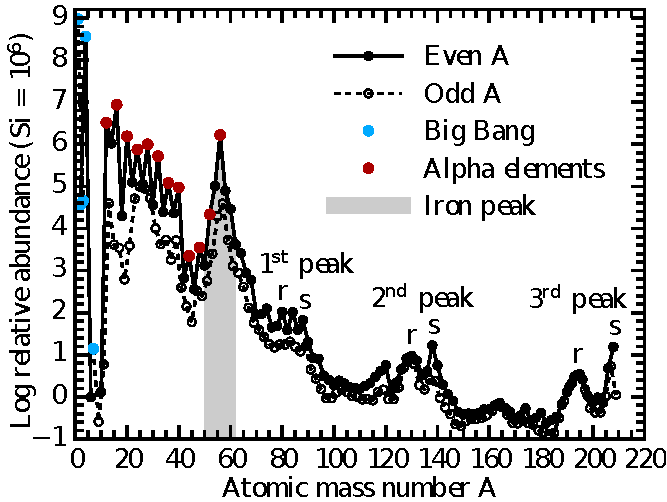
\includegraphics[width=0.49\textwidth]{Fig_1_1_Lip.pdf}
    \caption{Observed abundances in our solar system as a function of mass number
        $A$. The lightest elements were created in the Big Bang and fusion in stars predominantly
        creates alpha elements. The iron peak is made in core-collapse and type
        Ia \acp{SN}. Elements beyond the iron peak are synthesized by the slow ($s$) and
        rapid ($r$) neutron capture processes. These processes produce three distinct double
        peaks. Abundance data from \citet{Lodders:2003}. (Adapted from \citet{Lippuner:2018phd})
    }
    \label{fig:nuc:fig11_lip}
\end{figure}

%\begin{sidenote}
%    \textcolor{red}{Figure with solar observed abundances, showing $r$-elements and $s$-elements}
%    The observed obundacnes as a function of atomic mass number $A$ are shown in figure Fig. (XXX). 
%(data from \cite{Lodders:2003}). The plot shows nuclei that are more bound (due to spin pairing of nucleons 
%\cite{Moller:1993ed}), \textit{i.e,} those with an even $A$ number, are more abundant. The lowest binding 
%energy of nuclei with odd number of neutrons and protons (but even $A$) are largely unstable or short-lived. 
%A few exceptions are \textit{e.g.,} $^{40}$K, $^{50}$V, $^{138}$La and $^{176}$Lu, 
%that have a half-life of at least $10^{9}$ years.
%\end{sidenote}

The dominant \nuc{} process, responsible for the production of elements, varies with the mass 
number $A$.
%
For instance, light elements $A<8$ were synthesized right after the Big Bang
in the process known as \ac{BBN}.
Nuclides before the iron peak, $12\leq A\leq 56$ come from stellar hydrostatic 
nuclear burning \citep[\eg][]{Rolfs:1988,Hasen:2004}.
Elements at the iron peak $50\leq A \leq 62$ produces mostly 
during the type Ia \acp{SN} or explosive silicon burning in \acp{CCSN} \citep[\eg]{Woosley:2002}. 
The conditions at these sites are such that the dense material at the \ac{NSE}\footnote{
    At \ac{NSE} three parameters describe the composition: 
    density, temperature and electron fraction, $Y_e = n_p/(n_p + n_e)$, 
    where $n_e$ and $n_p$ are the (total) number density of electrons and protons 
    respectively \citep{Seitenzahl:2009}. 
    The composition at \ac{NSE} favors more tightly bound nuclides,
    as they are more difficult to photodissociate.
}, 
expands and cools down, enriching the \ac{ISM} with heavy elements \citep{Iwamoto:2000as}. 
%
%Most of the material beyond iron peak are produced via neutron capture processes 
%\citep{Burbidge:1957}.
Nuclides with $A\geq 56$ cannot be synthesized via standard cycles due to their 
strong Coulomb barriers. 
Thus, processes that do not involve charged particles become dominant. 
These are the neutron capture processes \citep{Burbidge:1957}.


%% -------------------------------------------------------
%%                   Nucleosynthesis Cites
%% -------------------------------------------------------

%\subsection{Nucleosynthesis up to the iron peak}
%
%
%\subsubsection{Big Bang nucleosynthesis}
%
%Light elements in the Universe, like hydrogen ($\sim 75\%$ by mass) and helium 
%($\sim 25\%$ by mass) alongside trace amounts of $^{3}$He and $^{7}$Li were created 
%during the \ac{BBN} (see \eg, \citet{Tytler:2000qf} and references therein). 
%And while only a small number of nuclides were involved in \ac{BBN}, 
%there are large discrepancies between \ac{BBN} models and observations. 
%For instance, the "lithium problem" \citep{Coc:2013eha}, which origin is not well 
%understood \citep{Fields:2011zzb}.
%
%
%\subsubsection{Low-mass stellar burning}
%
%In order to fuse massive nuclides and overcome the strong Coulomb barrier, high temperatures, 
%($\geq 10^6$ K) are required. Thus production of heavy elements from hydrogen and helium 
%is possible only in special environments, in particular, in the interior of stars 
%\citep{Bethe:1939}. 
%For the most of their lives stars burn hydrogen into helium. The process releases the 
%binding energy and maintains the hydrostatic stability of a star. After the hydrogen is 
%exhausted in the core, a core (atmosphere) contracts (expands), heats up (cools), and the 
%shell hydrogen burning is initiated, slowly depositing ashes, \eg, helium, into the inert core. 
%The star's subsequent evolution depends primarily on its mass. If the mass of a star 
%$M>0.5M_{\odot}$, at some point the helium in the core starts to fuse into $^{12}$C and 
%$^{16}$O and small amounts of $^{24}$Mg, $^{28}$Si. These elements are called 
%\textit{alpha elements} \citep{Rolfs:1988,Hasen:2004}. 
%The end of the core helium burning phase leads to another core contraction phase. 
%A star of a mass $\sim 8M_{\odot}$ would be able to ignite carbon and oxygen producing 
%heavier elements afterwards. A less massive star looses its outer layers and becomes a 
%slowly cooling degenerate core, a white dwarf.
%
%
%\subsubsection{nuclear burning is massive stars}
%
%For a star that has $M\geq 8M_{\odot}$, a sequence of burning stages follows, each of 
%which leads to the exhaustion of a respective fuel, contraction of the core and rise of 
%its temperature \citep{Woosley:2002}. Carbon burning leads to the production of 
%$^{20}$Ne, $^{23}$Na and free protons that contribute to the synthesis of non-alpha elements. 
%As temperature increases, the photodisintegration of $^{20}$Ne becomes possible and a small 
%amount of $^{24}$Mg is formed. Next, the oxygen burning occurs producing $^{28}$Si $^{31}$P, 
%and $^{28}$Si and $^{32}$S, that become dominant nuclides in the core by the end of oxygen burning \citep{Rolfs:1988}.
%
%The subsequent silicon burning proceeds at $T\sim3.5\times10^9$K through photodissociation 
%of some of the $^{28}$Si and a sequence of alpha particle captures, "alpha ladder", on the 
%remaining $^{28}$Si to form $^{32}$S, $^{36}$Ar, $^{40}$Ca, $^{44}$Ti, $^{48}$Cr, $^{52}$Fe 
%and $^{56}$Ni. This process lasts around a day \citep{Rolfs:1988,Hasen:2004}. Due to high 
%temperatures present at silicon burning, nuclides with $A\in[28, 62]$ fall into quasi-equilibrium, 
%meaning that these nuclides (with exception of $^{12}$C, $^{16}$O $^{20}$Ne and $^{24}$Mg), 
%alpha particles and protons participating in reactions, are in equilibrium with each other. 
%
%At $A=56$ the binding energy per nucleon appears reaches its maximum and the silicon burning 
%cannot produce heavier nuclides with the release of energy. As the fraction of $^{56}$Ni in the 
%core of a star increases, the support that nuclear burning has provided against gravitational 
%contraction falls. Meanwhile the mass of the degenerate core still increases as burning proceed in shells.
%However, when the electron degeneracy pressure can no longer counteract gravity, \ie, when mass 
%of the core exceeds the effective Chandrasekhar mass\footnote{
%    The collapse however occur before the core reaches Chandrasekhar mass, and the pressure 
%    support that rests on the availability of free electrons drops when electrons capture on 
%    the nuclides becomes possible. To account for this, the effective Chandrasekhar mass was 
%    introduced.
%}, 
%the core collapses leading to a \ac{CCSN} \citep{Woosley:2002}.
%Thus, the origin of more abundant alpha elements in the Universe is stellar fusion.
%
%
%\subsubsection{Iron Peak}
%
%At temperatures higher then $T\sim 5\times10^{9}$K nuclear \ac{NSE} establishes. This is a 
%balance between the fusion reactions forming a ($N,Z$) nuclide from $N$ neutrons and $Z$ 
%protons and photodissociation reactions, splitting it back. 
%At \ac{NSE} three parameters describe the composition: density, temperature and 
%electron fraction $Y_e = n_p/(n_p + n_e)$, where $n_e$ and $n_p$ are the (total) 
%number density of electrons and protons respectively \citep{Seitenzahl:2009}. 
%%
%The composition at \ac{NSE} favors more tightly bound nuclides, as they are more difficult 
%to photodissociate. Thus, if the conditions allow, \ie, temperature, density and electron 
%fraction of the mater, ($Y_e \sim 0.46$, an electron fraction of iron), nuclides at $A\sim56$, 
%\ie, iron peak elements, dominate \citep{Seitenzahl:2009}. 
%%
%For example, \ac{NSE} establishes during the type Ia \acp{SN}, when a thermonuclear 
%explosion of a white dwarf allows for sufficiently high temperatures and densities. 
%After the explosion, newly synthesized elements of the iron peak cools, and being stable, 
%remain in the expanding medium \citep{Iwamoto:2000as}.
%
%
%\subsection{Nucleosynthesis beyond the iron peak}
%
%Nuclides with $A\geq 56$ cannot be synthesized via standard cycles due to their strong Coulomb 
%barriers. Thus, processes that do not involve charged particles become dominant. 
%These are the neutron capture processes.
%%
As nuclides absorb neutrons and grow larger, their binding energy, $Q_n$, decreases. 
This process stops when $Q_n\sim1$~MeV and energetic photons start to knock out 
neutrons from a nucleus. This process is called photodisintegration and its location 
in the parameter space, (that in turn dependents on temperature and density), is called 
the 
%% [IMPORTANT]
neutron drip line 
%% ---
\citep{Rolfs:1988}.

Nuclides produced via neutron capture are generally unstable to $\beta$-decay, with a timescale, 
$\tau_{\beta}$, that can be larger or smaller than a neutron capture timescale, $\tau_n$. 
In case when $\tau_{\beta}\ll\tau_n$, \ie, when a $\beta$-decay occurs faster then the next 
neutron capture, the process is called \textit{slow} or \sproc{}. 
Thus, by definition, the \sproc{} moves along the valley of stability\footnote{
    a region of stable nuclides in the nuclides chart (a chart in terms of 
    number of neutrons $n_n$ 
    and number of protons $n_p$).
}, departing no further than by a few nuclides away.
On the other hand, if $\tau_{\beta}\gg\tau_n$, \ie, when a neutron capture occurs much 
faster then a $\beta$-decay, the process is called \textit{rapid} or \rproc{}. This \nuc{} 
generates nuclides near (but not crossing) the neutron drip line 
(See Fig.~\ref{fig:nuc:fig16_lip}) \citep{Rolfs:1988}. 

\begin{figure}[t]
    \centering
    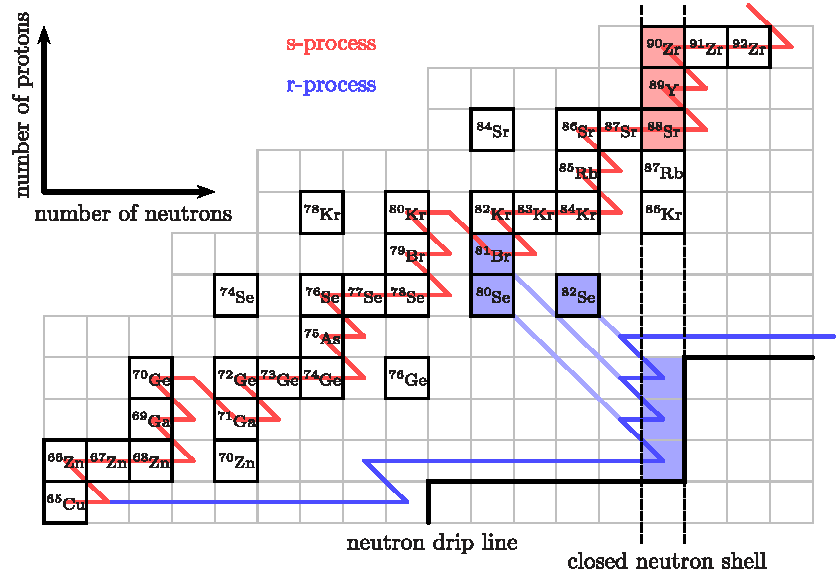
\includegraphics[width=0.60\textwidth]{Fig_1_6_Lip.pdf}
    \caption{Schematic representation of the $s$- and $r$-process on a section of the
        chart of nuclides. The \sproc{} (red) proceeds along the valley of stability and the
        \rproc{} (blue) along the neutron drip line. At the closed neutron shell $N = 50$, the
        neutron capture cross section drops by several orders of magnitude, which leads to a
        pile up of material there that produces the double-peak features
        (Adapted from \citet{Lippuner:2018phd})
    }
    \label{fig:nuc:fig16_lip}
\end{figure}

%% --- IMPORTANT --- ORIGIN OF THE PEAKS IN r-PROCESS
Notably, the trajectory of \rproc{} is interrupted when the neutrons within a nuclide can arrange 
themselves in a closed shell. Such configurations are energetically very favorable and thus the 
cross-section for a subsequent neutron capture reduces. Only after several $\beta$-decays does the 
\rproc{} continue. Thus, nuclides located at points where neutron drip line and a closed neutron 
shell overlap is more abundant. These unstable nuclides will decay back to the valley of stability 
and some of the neutrons within them turn to protons, reducing the total mass. The indication 
of this "overproduction" are the peaks in the abundance patterns at a mass, $A$, slightly lower then 
the one corresponding to a closed shell nuclide (see Fig.~\ref{fig:nuc:fig11_lip}).
%
%%% --- important
A similar "overproduction" of nuclides with a closed neutron shell occurs for the \sproc{}, 
%However, in that case it is caused by the cross section of these nuclides being 
%$1-2$ order of magnitude smaller then of neighboring ones \citep{Rolfs:1988}. Thus, in the case of 
%\sproc{}, 
but the peaks in abundance pattern will be at $A$, corresponding to the closed shell exactly, 
and thus located at larger $A$ than that of the \rproc{}. 
%
Closed shell nuclides are located at 
$N=50,\: 82, \: 126$ and thus corresponding abundance peaks for \sproc{} are at 
$A=88, \: 138, \: 208$ and at $A=80,\:130,\:194$ for \rproc{} (see \eg, \citet{Arnould:2007gh}) 
(See peak structure in Fig.~\ref{fig:nuc:fig11_lip}).

%% --- Motivation MP stars --- THE GENERIC SOLAR ABUNDANCES
%It was found, that the solar \rproc{} abundance pattern is general, and can be found anywhere in the 
%Universe: in stars that were formed very early on a galactic evolution timescale, \ac{MP} halo stars,
%that naively speaking, should not have had enough time to be formed out of material enriched by 
%\sproc{} and \rproc{} elements and show abundances similar to solar
%%For instance, in stars that were formed very early on a galactic evolution timescale, the 
%%\ac{MP} halo stars, one would expect to observe less \sproc{} and \rproc{} elements as there might have 
%%been not enough time for the enrichment to take place. However recent studies showed that the solar 
%%\rproc{} abundances are present in these stars as well 
%\citep{Sneden:2008,Roederer:2010}, 
%See also Fig.~$8$ in \citet{Sneden:2009}. 
%%Thus, modeling the \rproc{} \nuc{} it is expected to reproduce the solar abundances.

%%% -- can be deleted
%It is important to note that in addition to \sproc{} and \rproc{}, a possible $i$-process, (intermediate) 
%is widely discussed. The process operates further from the valley of stability than \sproc{}, but not 
%reaching neutron drip line \citep{Cowan:1977,Bertolli:2013gka}. Slow and intermediate neutron capture 
%processes operate within the low-mass \ac{AGB} stars with mass $M\in[1.5,3]M_{\odot}$ and more massive stars,
%that enrich the interstellar medium with heavy elements via strong winds 
%\citep[\eg][]{Peters:1968,Couch:1974,Kaeppeler:1994K,Woosley:2002,Straniero:2005hc,Herwig:2011}. 
%The possible cites for the \rproc{} we discuss in the following subsections.


\subsubsection{Possible $r$-process sites}

Study of possible cites of \rproc{} is a wide and rapidly developing field. The general requirement 
for \rproc{} is a low electron fraction, or, in other words, neutron-rich conditions. These can be 
found in various places for certain models of Big Bang, that include inhomogeneities, 
\ac{BNS} and \ac{NSBH} mergers and \ac{SN} ejecta (see \citet{Mathews:1990} and references therein). 
%
Spectral studies of \ac{MP} stars (formed early in the galactic history), combined with models of 
galactic chemical evolution sheds light on possible dominant cite of \rproc{} material. 
%\textcolor{red}{add more sources/models}. 
It is now believed that certain types of \acp{SN} and \ac{BNS} mergers are the most likely 
sources on \rproc{} material \citep{Mathews:1990,Thielemann:2011,Siegel:2019mlp} %\textcolor{red}{add more sources}


%\subsubsection*{\acp{CCSN}}

Collapse of a massive star produces a hot neutron core, that undergoes deleptonization, releasing 
$\sim10^{53}$~erg of binding energy in a form of strong neutrino flux. These neutrinos, irradiating 
dense medium around the core, can produce a \nwind{} \citep{Qian:1996xt}, that was suggested to be 
a promising cite for \rproc{} \citep{Woosley:2002,Wanajo:2006mq}. Later, it was shown however, that 
the electron fraction in the wind would be too high for a full \rproc{}, and only ``light'' heavy 
nuclide, up to $A\sim130$, can be synthesized 
\citep{Qian:1996xt,Thompson:2001ys,Fischer:2010,Roberts:2010,MartinezPinedo:2012rb,Wanajo:2013} 
%\textcolor{red}{add Perego:2017} 
%
%It is important to note that in the proton-rich \nwind{} nuclides with $A\sim 100$ can be produces 
%via so-called $\nu p$-process. The process relies on a creation of a free neutron from proton by 
%an antineutrino capture. These free neutrons can then be captured by a seed nuclide, $^{64}$Ge seed 
%nuclide and thus nuclides heavier then $^{64}$Ge can be created
%\citep{Frohlich:2006,Pruet:2005qd,Wanajo:2010mc,Arcones:2012}
%
A full \rproc{} can be achieved in so-called magnetorotationally driven \acp{CCSN}. 
This is a rare type of \acp{CCSN}, where a core of the progenitor is rotating rapidly 
and is strongly magnetized. Induced by a magnetorotational processes \eg, \ac{MRI}, 
collapse is accompanied by a formation of a collimated bipolar jet 
\citep{Wheeler:2000,Akiyama:2003,Burrows:2007yx,Mosta:2014jaa,Mosta:2015,Siegel:2019mlp}.
Materiel in these jets is predicted to be sufficiently neutron rich to allow for a full 
\rproc{} \nuc{} \citep{Winteler:2012,Nishimura:2015nca}. The rarity of this type of \acp{SN}, 
however, might not allow for them to be the dominant source or \rproc{} material 
\citep{Nishimura:2015nca} 

%Mergers of \acp{NS} we discuss separately in Sec.~\ref{sec:intro:bns_ejecta}

%\subsubsection{Compact object mergers}
%\red{TO BE REWRITTEN -- REPETITION OF PREVIOUS CHAPTERS}


%% --- MIGHT NEED TO BE SHORTENED A LOT!  OR MOVED TO INTRODUCTION!
Mergers of two \acp{NS} or a \ac{NS} and a \ac{BH} are regarded as one of the main cites 
of \rproc{} material (See Sec.~\ref{sec:intro:bns_merg}). 
%Compact objects, formed in a binary evolution of massive stars, 
%orbit each other for gigayears, before slow loss of energy from the system due to \acp{GW} 
%reduces their orbit and they merge \citep[\eg][]{Hulse:1975,Lattimer:2004sa,Price:2006fi}. 
%
%The late inspiral and merger of \ac{BNS} or a \ac{NSBH} have been studied extensively via smooth particle 
%simulations \red{[REFS]} \ac{HD} simulations \red{[REFS]} and \ac{NR} simulations with simplified gravity \red{[REFS]} 
%or full \ac{GR} \red{[REFS]}. The composition of a \acp{NS} in these simulations have been modeled with 
%simplified polytropic \red{[REFS]} or piece-wise polytropic \red{[REFS]} or microphsyical \acp{EOS} \red{[REFS]}. 
%The physical setup of these simulations have also evolved to eventually include effects of
%neutrino radiation transport \red{[REFS]} and magnetic fields \red{[REFS]}. 

%These studies have shown that shortly before and during the merger, the neutron star(s) undergo(s) a tidal 
%deformation and disruption. Streams of neutron-reach matter are then ejected into the circombinary 
%with enough energy to be not graviationally bound to the system \citep{Price:2006fi,Foucart:2014nda,Sekiguchi:2015dma,Kyutoku:2015gda,Radice:2016dwd}. 

%% For details on the ejecta from \ac{BNS} mergers see Chapter \ref{ch:BNS_results}.
%% In addition, in case of a \ac{BNS}, when \acp{NS} collide, material at the collision interface, heated by shocks, 
%% gets 'squeezed' and launched in the directions perpendicular to the plane of the binary \cite{Bauswein:2013,Hotokezaka:2013b} \red{[REFS]}. 
%% Generally, these tow components, tidal and shocked, constitute the \textit{dynamical ejecta}. Where the term 
%% ejecta referrers to the material that has enough energy to leave the system. 
%% The properties of the dynamical ejecta from BNS have a broad distribution, especailly in terms of mass and ejectron fraction 
%% [\red{[REFS]} \& myFitPaper], where the former lies in range $(10^{-4},10^{-2})M_{\odot}$ and the latter $(0.05,0.45)$. 
%% We discuss dynamical ejecta properties of BNS in more details in section \red{sec:results:dyn\_ej:prop} and nucleosynthesis 
%% in it in \red{sec:results:dyn\_ej:nucleo}. In case of NSBH the ejecta mass was shown be larger, reaching $0.1M_{\odot}$ with 
%% low electron fraction, $\leq0.2$ but it requires that masses of BH and NS are comparable and BH is rapidly spinning 
%% \cite{Foucart:2014nda}\red{[REFS]}. If the BH is much more massive then NS, the latter would be 'swallowed' with no ejecta \red{[REFS]}.
%% After the merger, there are expected to be additional ejecta. For general postmerger configuration consists of a remnant, massive neutron 
%% star (MNS) or a black hole sorrounded by a disk (torus) of bounded matter. In the first case,  a strong neutrino flux from cooling MNS and 
%% disk can drive an outflow in the direction, perpendicular to the plane of the binary, the so-called \nwind{} 
%% (see Figure 1 from \cite{Perego:2014fma}) \red{[REFS],Jujibayashi+20}. This ejecta is expected to occure on a timescales of 
%% $\sim100$ms postmerger, be not very neutron rich $Y_e\sim(0.2-0.45)$ due to neutrino irradiation and have a mass of 
%% $(10^{-4}-10^{-3})M_{\odot}$ \red{[REFS]}. 
%% The massive nutron star born in a merger exhibit dynamical oscillations \red{[REFS]}. The $m=1$ mode, so-called 
%% "one-armed spiral instability" especially can persisit on a $\sim100$ms powtmerger timescale and become a dominant mode 
%% \red{[REFS], MainPaper}. This oscillations can inject energy within the disk, where via angular momentum transport it leads 
%% to an outer part of the disk to become unbound. This ejecta, the \textit{\swind{}} was shown to occur in all cases where the MNS is present. 
%% It has high electron fraction and its mass depends on a lifetime of the remnant, and for a $\sim100$ms it can amount to a few 
%% $\times\sim10^{-2}M_{\odot}$ \red{[Letter, MainPaper]}. We discuss the mechanism that drives the \swind{} in the section 
%% \red{sec:results:swind:mechanism} and the ejecta properties in \red{sec:results:swind:prop} and corresponding 
%% nucleosynthesis in \red{sec:results:swind:nucleo}.
%% On a longer timescales, the viscous processes and alpha recombination in the disk, surrounding MNS or a BH are expected 
%% to unbind additional material. This is so-called \textit{secular ejecta}. It is expected to be massive and neutron rich. 
%% However, due to long timescales involved, it is very difficult model \red{[REFS]}.

\ac{BNS} and \ac{NSBH} mergers eject neutron rich material 
in which \rproc{} can take place, producing nuclides beyond $A=300$. Over-saturated with neutrons, 
nuclei are unsubtle to fission, and decay shortly after being formed. The decay products, 
before they reach the valley of stability, capture again free neutrons and grow up to 
$A=300$ and the cycle repeats. 
%% -- important 
This is so-called fission cycle. %\red{might be better to remove it from here and discuss later}
%\subsubsection{Fission cycling}
%Fission cycling is a process where freshly synthesized via strong \rproc{} heavy nuclides 
%with $A\sim 300$ undergo fission just to become seed nuclides for a similar \rproc{} 
%leading to an $A\sim 300$ nuclide. 
%This process eliminates the dependency of the final abundances on the initial conditions and 
%it also limits the maximum nuclide mass that can be achieved. 
%%
%The number of fission cycles can be estimated via a ration of the seed nuclides at time 
%zero and the number of seeds at the time when there are no more free neutrons available. 
%This is motivated by the fact that neutron capture itself does not create new seeds, only
%increases the mass of them, while fission, splitting heavy nuclide in two, generates 
%additional seeds. 
%%
%The number of fission cycles is tight to how much lanthanides and actinides are produced. 
%In particular, as fission cycling limits the maximum mass of the nuclide that can be created, 
%the fraction of lanthanides, actinides as well as heating $\varepsilon$ are insensitive 
%to the initial $Y_e$. The number of cycles is thus tight to the initial $Y_e$. The lower it is,
%the more free neutrons available and thus more cycles would occur. After the fission cycling
%stops the $r$-process maximum mass drops to $A\sim 250$. Thus the amount of actinides drops as
%only the lightest of them can be produced that do not fission immediately. 
%% --- 
It is maintained as long as there are free neutrons. After, the nuclides decay to the valley of 
stability for the last time, forming the remarkably robust abundance pattern, independent of the 
number of cycles \citep{Korobkin:2012uy,Bauswein:2013yna,Mendoza-Temis:2014mja}, 
(see also Figure 4 in \citet{Korobkin:2012uy}).
%
%Numerical models have shown that the final \rproc{} abundances in the \ac{BNS} and \ac{NSBH} 
%mergers ejecta are robust and reproduce the solar ones robustly 
%\citep{Freiburghaus:1999,Goriely:2011vg,Goriely:2015fqa,Wanajo:2014wha,Just:2014fka,Radice:2016dwd}\red{[Refs]}. 
%Recent observations of the one and only detected so far merger have confirmed that \ac{BNS} mergers do 
%produce \rproc{} elements \red{[Refs] incl. Stroncium paper}.


\subsubsection{Galactic chemical evolution}

While there are several generally accepted cites for the \rproc{}, the main one is yet to be 
determined \citep[\eg][]{Qian:2000bh,Argast:2003he,Matteucci:2014}
%
%%% DELAY
For instance, the observed \rproc{} enrichment of \ac{MP} stars 
%if \ac{BNS} mergers are the main cite, than 
%the observed \rproc{} enrichment is difficult to explain as it 
requires very early source of \rproc{} material, when no mergers 
should have had happened yet, as the inspiral time ads the time delay of order 
%This time delay before the compact binary binary formation and merger is 
$10^{6} - 10^{9}$ years \citep{DeDonder:2004cx,Dominik:2012kk}, and is highly uncertain and 
depends on a poorly understood common envelop evolution phase of the massive binary (progenitors)
\citep[\eg]{Dominik:2012kk}. 
%%%% SCATTER
Additionally, mergers of compact objects are rare events and thus expected to introduce 
a considerable scatter into the \rproc{} elements distribution in the Galaxy. 
However, observations show that the distribution is more uniform than expected \citep{Argast:2003he}.
%%%% CCSN as a contributor
Recent population synthesis models have indicated that with a contribution from 
magnetorotationallydriven \acp{CCSN} the compact object mergers can account for the 
observed scatter of heavy elements \citep{Ishimaru:2015,Cescutti:2015,Wehmeyer:2015,VanDeVoort:2015}.
%
%%%% --------------------------------
%%%% IN MORE  DETAILS 
%%%% --------------------------------
%%%% Delay
%After the \ac{BBN}, the Universe consisting of hydrogen and helium, with traces of lithium, have expanded and cooled. 
%Under the influence of dark matter, the primordial gas fragmented, clumped and first stars, galaxies and galaxy 
%clusters have formed. During their lifetime the first stars (population III stars) converted light elements into 
%heavier ones and then ejected them into the \ac{ISM} during \ac{SN} events. Future populations of stars were born 
%of gas enriched with heavy elements, in particular, iron. Thus, the amount of elements heavier then hydrogen and 
%helium is stars (\ie, metallicity) increased with each stellar generation and there exists an age-metallicity relation 
%\citep{Matteucci:2012}. Important to note, that multiple dark matter sub-halos contributed to the formation of the 
%galaxy and there might not be a unique age-metallicity relation (see \eg, \citet{Ishimaru:2015} and references therein).
%%% Delay
%The enrichment of interstellar medium with heavy elements from stellar interior occurs immediately after stars die. 
%However, the \rproc{} elements, produced in \ac{BNS} (\ac{NSBH}) mergers can only enrich \ac{ISM} when compact objects 
%inspiral and merge which on average takes $(0.1-1)\times10^{9}$ years \citep{DeDonder:2004cx,Dominik:2012kk}. 
%The exact delay time is however highly uncertain and depends on a poorly understood common envelop evolution phase of the binary 
%(progenitors). And it was shown, that a small percentage of compact binaries might form with a time delay 
%before merger as small as $10^{6}$ years \citep{Dominik:2012kk}. 
%
%%% Study observations
%To study the chemical evolution of stars in the galaxy, the spectroscopic surveys\footnote{
%    And indicative quantity of metallicity measured in such iron-to-hydrogen ration, [Fe/H], that reads as a $\log_{10}$
%    of the abundance of a element $X$ to hydrogen, normalized to solar ration, \ie, in the sun for every X, [X/H]$= 0$. 
%    If a stars has [Fe/H]$=-2$, it is said that this star ahs a 100 times less iron compared to hydrogen then sun.
%} are conducted \citep{Edvardsson:1993,Suda:2008na}. 
%%% Scatter
%Mergers of compact objects are rare events and thus expected to introduce a considerable 
%scatter into the \rproc{} elements distribution in the Galaxy. However, observations show that the 
%distribution is more uniform than expected \citep{Argast:2003he}.
%%% Scatter
%However, recent population synthesis models have indicated that with a contribution from 
%magnetorotationallydriven \acp{CCSN} the compact object mergers can account for the observed 
%scatter of heavy elements \citep{Ishimaru:2015,Cescutti:2015,Wehmeyer:2015,VanDeVoort:2015}.
%
%% 244Pu
Comparison between the solar system and earth crust abundances of $^{244}$Pu have indicated that this 
nuclide might have been produced in rare events with high yields \citep{Wallner:2015}. This statement 
was confirmed via models of galactic mixing \citep{Hotokezaka:2015zea}, that also showed that there 
appears to be no degeneracy between rare high yields events (\ac{BNS}/\ac{NSBH}) 
and frequent low yield ones (\ie, \ac{CCSN}). Similar conclusion was draws from studying $^{244}Pu$ 
abundances in meteorites \citep{Tsujimoto:2017}.
%
%% UFDG
Study of \acp{UFG} also point towards a rare high yield events for \rproc{} \nuc{}. In particular, 
the \ac{UFG} Reticulum II was shown to have a solar \rproc{} abundances, while \ac{UFG} of similar 
type tend to have $2-3$ times less \rproc{} elements. This suggests that a rare high-yield event 
has modified Reticulum II chemical composition and high europium abundances indicate that it was a 
compact object merger \citep{Ji:2016}. 
%
%Thus it is still unclear whether observed degree of homogeneity in \rproc{} elements distribution in the galaxy and 
%\rproc{} elements enrichment of very \ac{MP} stars can be explained by compact object mergers only. 
%% Scatter

%\red{Mention Actinide abundaces problem.}

%% --------------------------------------------------------------------------
%%               K I L O N O V A
%% --------------------------------------------------------------------------

\subsection{Kilonova}

Nuclides, synthesized in \rproc{} are very neutron rich and unstable. After the last 
fission cycle, they decay to the valley of stability.% (see chapter~\ref{ch:nucleo}). 
%
%This process takes from hours to days and released energy 
%can power an \ac{EM} transient, called \ac{kN} or Macronova  
%\citep[\eg][]{Li:1998bw,Kulkarni:2005jw,Metzger:2010,Roberts:2011,Metzger:2016pju,Wollaeger:2017ahm}
%
%
%During the \ac{BNS} mergers, the neutron-rich material is ejected 
%(see Chapter \ref{ch:bns_sims} for details). The conditions of the eject are such that they allow 
%for the \rproc{}, that produces heavy elements far from the valley of stability (see Chapter 
%\ref{ch:nucleo} for details) 
Li et al., \citep{Li:1998bw} suggested that an \ac{EM} transient can be powered by 
the radioactive decay of the material enriched with \rproc{} elements, ejected in 
\ac{BNS} or \ac{NSBH} mergers. They also showed that contrary to the normal \acp{SN}, 
the ejecta would quickly become transparent to its own emission, peaking on a timescale 
of around a few days. The main difficulty in this pioneering work was the lack of a \nuc{}
 model to model to estimate the radioactive heating of the ejecta. 
%
The understanding of \ac{kN} has significantly improved since then
\citep[\eg][]{Kulkarni:2005jw,Metzger:2010,Roberts:2011,Metzger:2016pju,Wollaeger:2017ahm}
%
but the only unambiguous detection of \ac{kN} so far, was the thermal transient, \AT{}, 
\citep{Coulter:2017wya,Chornock:2017sdf,Nicholl:2017ahq,Cowperthwaite:2017dyu,Tanvir:2017pws,Tanaka:2017qxj}
that was observed after the \ac{GW} trigger, \GW{}, 
\citep{TheLIGOScientific:2017qsa,Abbott:2018wiz,LIGOScientific:2018mvr}.
%
This observation provided evidences that the ejection of neutron-rich matter from compact 
binary mergers is one of the primary site for \rproc{} nucleosynthesis 
%\citep{Lattimer:1974slx,Li:1998bw,Kulkarni:2005jw,Rosswog:2005su,Metzger:2010,Roberts:2011,Kasen:2013xka}.
\citep{Arcavi:2017xiz,Coulter:2017wya,Drout:2017ijr,Evans:2017mmy,Hallinan:2017woc,Kasliwal:2017ngb,
    Nicholl:2017ahq,Smartt:2017fuw,Soares-santos:2017lru,Tanvir:2017pws,
    Troja:2017nqp,Mooley:2018dlz,Ruan:2017bha,Lyman:2018qjg}. 
%The \ac{kN} is the \ac{EM} \ac{UV}/optical/\ac{NIR} transient, powered by the 
%radioactive decay of the elements synthesized via \rproc{} in expanding ejecta.
%
The peak in \ac{NIR} band of \AT{} occurred several days after the merger \citep{Chornock:2017sdf}.
It is generally consistent with emission from the high opacity material, with a sizable 
fraction of lanthanides \citep{Kasen:2013xka}
%
The peak in \ac{UV}/optical band, however, occurred in less than one day after the merger 
\citep{Nicholl:2017ahq}. This requires the opacity of the material to be sufficiently low, 
suggesting that only partial \rproc{} \nuc{} took place in the corresponding ejecta 
\citep{Martin:2015hxa}.
%
These observations that material with distinctly different properties contributed to the emission.
%
% [RED]
%\ac{kN} has a complex observational signature due to different ejecta components with various 
%compositions contribution to it. 
In particular, it was shown that if produced, 
lanthanides $(58\leq Z \leq71)$ and actinides $(90\leq Z \leq 103)$ with their open 
$f$-shell and hence a plethora of absorption lines, increase opacity of emitting 
region by a factor of $10$. 
%
These elements are produced only if electron fraction of the ejecta was sufficiently low, 
$Y_e\leq 0.25$ \citep{Lippuner:2015gwa}, present for example in a tidal component of \ac{DE}. 
High opacity would imply that a transient is dim $(\sim10^{40})$ erg s$^{-1}$ and peak around a 
weak after merger in the red/infrared band \citep{Barnes:2013wka,Grossman:2013lqa,Lippuner:2015gwa}. 
%
% [BLUE]
If the ejecta electron fraction is high, $Y_e \geq 0.25$, weak \rproc{} would produce a small amount 
of lanthanides and the opacity of the emitting region would thus be lower. The kilonova signal originating 
from such ejecta would be bright and peak on a timescale of a few days in blue band 
\citep{Kasen:2014toa,Martin:2015hxa}. 
%
%
Indeed, both and red components were observed in the case of \AT{}, that confirmed the general 
picture \citep[\eg][]{Villar:2017wcc}. However, estimated mass of the ejecta required to explain 
the red component is larger then what is predicted by numerical relativity simulations \red{refs}. 
It is believed that the most contribution to this component comes from the low $Y_e$, slow but 
massive outflow from the degenrate disk on a secular timescale \red{refs}.
%
Semi-analytic two-components (red and blue) spherical \ac{kN} models to the \AT{} observations 
provided estimates for the ejecta properties for these two components. 
%
Specifically, for the langhinide poor (rich) \ie, blue (red) components, the required mass is 
$2.5\times10^{-2}M_{\odot}$ ($5.0\times10^{-2}M_{\odot}$) and velocity $0.27$c ($0.15$c)
\citep{Cowperthwaite:2017dyu,Villar:2017wcc}. 
See however \citep{Waxman:2017sqv} for an alternative interpretation.
See also \citep{Siegel:2019mlp} for the compiled data on the \ac{kN} models.
%
Similar estimates are obtained with $1$D radiation transport \ac{kN} models
\citep{Tanvir:2017pws,Tanaka:2017qxj}.
%
%A very high energy emission from the non-thermalized radiation is weak and can be 
%detected only for a sufficiently close event \cite{Hotokezaka:2015cma}.
% 
Notably, prior to \AT{}, there were other candidates based on the detection of \ac{SGRB}, 
with infrared excess \eg, 
GRB130603B, \citep{Berger:2013wna,Tanvir:2013pia}, 
GRB060614 \citep{Jin:2015txa,Yang:2015pha}, 
GRB050709 \citep{Jin:2016pnm}.
GRB200522A \citep{WRONG}  Bruni:2021ilp
However the exact nature of the observed signals were not well constrained. 
%
The search for \ac{EM} counterparts to mergers continues, involving observatories around the world 
\citep{Law:2009,Singer:2014qca,Bellm:2014,Kasliwal:2016uhu}.

%% --------------------------------------------------------------------------
%%               A F T E R G L O W S
%% --------------------------------------------------------------------------

\subsection{$\gamma$-ray bursts and kilonova afterglows}

\acp{GRB} are irregular pulses of gamma-ray radiation with broken power-law 
(non-thermal) spectrum, peaking at KeV-MeV \citep{Band:1993,Kouveliotou:1993,Meegan:1992xg}.
%
With respect to the duration, \ac{GRB} are split into two categories: \ac{SGRB}, 
that last ${\leq}2$~s and long \ac{GRB} that last ${\gtrsim}2$~s. The latter are the 
result of the collapse of massive ${\geq}15M_{\odot}$ stars, while the former, at 
least in part, is attributed to mergers of compact objects. Only very recently it 
was directly confirmed with the detection of \ac{SGRB} \GRB{} that accompanied 
the \ac{GW} event \GW{} \citep{TheLIGOScientific:2017qsa}. However, the exact physical 
origin of different duration \ac{GRB} is not fully understood.
%
Indications that long \ac{GRB} are associated with core-collapse supernovae, \acp{SN}, 
are two fold. These \acp{GRB} are typically observed in star-forming regions of their 
host galaxies \citep[\eg][]{Bloom:2000pq,Bloom:2002hc,Fruchter:2006py,Christensen:2004yx,CastroCeron:2006jh} 
and several \acp{GRB} are spectroscopically associated with Type Ic \acp{SN}, albeit 
these \acp{GRB} were significantly less bright and might not be typical \acp{GRB} 
\citep[\eg][]{Liang:2006ci,Bromberg:2011fm}. Additionally, the late time behaviour 
of some \acp{GRB} includes a \acp{SN}-like "bump" in the optical and spectral changes 
that might imply that underlying \acp{SN} flux becomes dominant over \acp{GRB} 
\citep[\eg][]{Bloom:1999,Woosley:2006fn}.
%
The \acp{GRB} are distant events, most of which were localized to outside the local 
group \citep[\eg][]{Mao:1992,Piran:1992,Fenimore:1993}. Particularly useful for distance 
estimation were the observations of \ac{GRB} afterglow, fading X-ray \& optical emission, 
that allow to estimate the redshift \citep[\eg][]{Costa:1997cg,Frontera:1997ae}.
%
Analysis of the multi-wavelength afterglow data for \acp{GRB} \citep[\eg][]{Panaitescu:2001bx} 
suggested the mechanism behind the afterglow emission is the synchrotron radiation from the 
external forward-shock, which forms when \ac{GRB}-ejecta sweeps-up the \ac{CBM} or \ac{ISM}
medium\footnote{
    The specific indications are the power law decay of the light curves, 
    $F_{\nu}\propto^{-1}$ and power-law spectrum $F_{\nu}\propto\nu^{-0.9\pm 0.5}$.
} 
\citep{Rees:1992ek,Paczynski:1993gz,Meszaros:1993ju,Meszaros:1996sv}.
%
The temporal behavior of many (but not all) \acp{GRB} shows a change, a steepening 
of the light-curve (to $F_{\nu}\propto t^{-2.2}$) at $\sim 1$~day after the burst. 
This is usually attributed to the 
%\gray{deceleration of the colimated GRB-outflow, jet, and decrease on the realtivisitc beaming. This in turn makes the edge of the jet visible to an observer.} 
finite angular extend of the \ac{GRB}-ejecta, jet \citep[\eg][]{Rhoads:1999wm,Sari:1999mr}. 
When jet decelerates and relativistic beaming decreases (and the jet edge becomes visible), 
the optical and X-ray lightcurves decay achromatically faster. This achromatic transition 
from slow to faster decay is called "jet-break".
%
%%% PROBLEMO -- jet-break is not a universal feature.
%Notably, this jet-break is not observed in all \acp{GRB} for the reason that is not fully 
%understood \citep[\eg][]{Fan:2006pj,Panaitescu:2006,Liang:2007ti,Sato:2006jg,Liang:2007rn,Curran:2007cp,Racusin:2008bx}
%%
%%% PROBLEMO -- GRB density seems uniform, but SSE models predict wind-like profile
%Models of the broadband emission of \acp{GRB} with jet-break showed that the 
%\ac{CBM}, is uniform with number density \red{$\sim 10^{-3}$} \citep{Panaitescu:2001bx}. 
%If \acp{GRB} produced in collapse of massive stars \citep{Woosley:1993,Paczynski:1997yg}, 
%this contradicts the expected density profile from stellar winds, \eg, $\rho\propto r^{-2}$ 
%\citep[\eg][]{Dai:1998iz,Chevalier:1999jy,Chevalier:1999mi,Ramirez-Ruiz:2001} 
%\red{this might be very outdated.}
%
%% sGRB
The origin of \acp{SGRB} was first connected with the elliptical galaxes, and with 
older stellar population 
\citep[\eg][]{Gehrels:2005qk,Fox:2005kv,Barthelmy:2005bx,Berger:2005dr,Panaitescu:2005er,Bloom:2005qx,Guetta:2005bb,Nakar:2007yr} 
and thus with \ac{BNS} mergers. A more direct evidence came with the \GRB{}
\citep{Savchenko:2017ffs,Alexander:2017aly,Troja:2017nqp,Monitor:2017mdv,Nynka:2018vup,Hajela:2019mjy}, 
detected by the space observatories Fermi \citep{TheFermi-LAT:2015kwa} and INTEGRAL \citep{Winkler:2011}.
%
Generally \acp{SGRB} show a complex time behavior of early afterglow X-ray emission, 
in particular a presence of a plateau ($F_{x}\propto t^{-1/2}$), after the initial sharp 
decrease ($F_{x}\propto t^{-3}$) which a standard forward shock model does not predict. 
This implies that early X-ray afterglow is shaped by a variety of physical processes 
\citep{Zhang:2005fa}.
%
The \GRB{} was dimmer then any other events of its class. 
Different interpretations for its dimness and slow rising flux were proposed: off-axis jet, 
cocoon or structured jet. Now it is commonly accepted that \GRB{} was a structured jet 
observed off-axis 
\citep[\eg][]{Fong:2017ekk,Troja:2017nqp,Margutti:2018xqd,Lamb:2017ych,Lamb:2018ohw,Ryan:2019fhz,Alexander:2018dcl,Mooley:2018dlz,Ghirlanda:2018uyx}.
The \GRB{} late emission, the afterglow, provided information on 
the energetics of the event and on the properties of the circumburst medium 
\citep[\eg][]{Hajela:2019mjy}. 

%%%% EARLY emission problem
%Two main questions stem from these observations: is the mechanism behind the prompt 
%$\gamma$-ray emission and early afterglow emission is the same (or do they originate from 
%the same outflow), and is the early X-ray radiation produced by the external shock (just a 
%blast wave takes long time to become self-similar) or does it originate from an internal 
%shock? An indication that the long-lived central engine activity might affect the 
%afterglow came from the observed sharp increase in X-ray flux (flares) on a 
%scale of minutes to hours after the end of the \ac{GRB}
%\citep{Burrows:2005ww,Chincarini:2007fp,Chincarini:2010,Margutti:2011}, 
%which could not be attributed to the inhomogeneities in the \ac{CBM}.
%%% PROBLEMO!
%Thus, the early X-ray behaviour of \acp{GRB} $t < 10^{4}$~s post-burst is not well 
%understood and seems to be in tension with standard afterglow forward shock emission model.

%\textcolor{red}{
%    One of the foremost unanswered questions about GRBs is the physical mechanism
%    by which prompt $\gamma$-rays the radiation that triggers detectors on board
%    GRB satellites are produced. Is the mechanism the popular internal shock
%    model 6 \cite{(Rees and Meszaros, 1994)}, the external shock model, or something
%    entirely different? Are $\gamma$-ray photons generated via the synchrotron process
%    or inverse-Compton process, or by a different mechanism? Answers to these
%    questions will help us address some of the most important unsolved problems
%    in GRBs  how is the explosion powered in these bursts? Does the relativistic
%    jet produced in these explosions consist of ordinary baryonic matter, electron positron
%    pairs, or is the energy primarily in magnetic fields?
%}

%Once again, while it is suggested that the high energy emission, after the propmt phase is produced 
%by the synchrotron process in the external forward shock, \citep{Kumar:2009,Ghisellini:2010}, 
%the mechanism behind the high and low energy $\gamma$-ray emission in the prompt phase remains unknown. 
%Possible mechanisms include: inverse Compton and synchrotron emission in internal and external shocks
%\citep[\eg][]{Rees:1992ek,Dermer:1998py,Lyutikov:2003ih,Zhang:2011} and 
%photospheric radiation with contribution from multiple \ac{IC} scatterings
%\citep[\eg][]{Thompson:1994zh,Ghisellini:1998jy,Meszaros:1999gb,Peer:2005qoc,Peer:2008udu,Giannios:2006jb,Ioka:2007qk,Asano:2009gi,Lazzati:2010,Beloborodov:2010,Toma:2011}.

%% from the Afterglow paper



%\subsection{kilonova afterglow}

In addition to the \ac{GRB} beamed emission, the non-thermal, more isotropic 
emission is expected from electrons accelerated in shocks formed between the 
(mildly) relativistic ejecta and the \ac{ISM} \citep{Nakar:2011cw}. This emission 
is expected to peak in radio band and continue on a time scale of tens of years 
after merger. Notably, all ejecta components will contribute to the emission, 
but depending on the ejecta velocities and kinetic energy, 
the brightness in different frequencies and timescales differs. 
%
Various ejecta components interact with each other and with \ac{ISM}. The latter, 
generates a long-lived blast wave. The shock, propagating upstream, amplifies 
(random) magnetic fields and accelerates electrons, that subsequently emit 
synchrotron radiation. This process in phenomenological similar to the for the 
\ac{GRB} afterglow and \ac{SN} early remnants. 
%
Numerical simulations of \ac{BNS} mergers showed the presence of mildly relativistic 
ejecta (See Sec.~\ref{sec:bns_sims:method:ejecta}). 
Several studies on the possible non-thermal electromagnetic emission of this ejecta 
have been carried out 
\citep[\eg][]{Piran:2012wd,Hotokezaka:2015eja,Hotokezaka:2018gmo,Radice:2018pdn}. 
Notably, the observed non-thermal emission from \GW{}, was first interpreted 
as the non-thermal emission from the ejecta \citep{Mooley:2017enz}.
This interpretation was however disproved by the emergence of jet break
%
%Specifically, a strong radio emission is expected from \ac{BNS} ejecta \citep{Piran:2012wd,Hotokezaka:2015eja}. 
The \ac{BNS} merger radio remnant is expected to peak on a time-scale 
of years after the merger and be visible over a similar timescale. Notably, this is 
assuming that the ejecta is expanding into the unshocked \ac{ISM}, as it was shown 
that if the \ac{ISM} is pre-shocked by the jetted outflow, and the \ac{ISM} density is 
reduced, the kilonova afterglow would be delayed. 
%
In \citet{Piran:2012wd}, the synthetic \ac{kN} afterglow \acp{LC} are calculated 
for a set of \ac{NR} \ac{BNS} merger simulation with properties typical to the 
Galactic binary population and \ac{ISM} density usually found in the Galactic disk, 
$\nism\sim1\ccm$. Authors showed that the from a binary of two $1.4\Msun$ \acp{NS}, 
the kilonova afterglow would peak $\sim10$~years after the merger if $\nism = 0.1\ccm$ 
and $\sim3$~years if $\nism = 1\ccm$ in radio bands, $\nu=1.4$~GGz and $\nu=150$~MGz. 
Notably, both values of the \ac{ISM} density are larger than what is inferred for \GW{}. 
Indeed, jet fitting models and dependent analysis of the diffuse emission suggest 
$\nism\in(10^{-4},10^{-2})$\gcm \citep{Hajela:2019mjy}.
%In \citet{Piran:2012wd} authors focus on the observational prospects of this afterglow 
%and compare it to other \ac{EM} emission expected for \ac{BNS}. 

%% =====================================================================================
%%
%%              T H E O R E T I C A L  P I C 
%%
%% =====================================================================================

\section{Theoretical picture of \ac{BNS} mergers}

In This section we briefly overview the current understanding of the \ac{BNS} 
merger, the dynamics of the inspiral, effects of tides, \pmerg{} hydrodynamics 
and open questions.

%% --------------------------------------------------------------------------
%%               I N S P I R A L
%% --------------------------------------------------------------------------

\subsection{Inspiral}

If \acp{NS} formed through a classical stellar evolution channel of the massive binary, 
their orbit is mostly circular with little to non eccentricity \cite{4}. 
%
The binary system looses energy to the emission of \acp{GW}, and the orbit of \acp{NS} 
shrinks. Stars inspiral. The last ${\sim}10^3$ orbits, for instance, can be completed in 
a matter of minutes. During the last part of the inspiral, the \ac{GW} signal rises in 
frequency and amplitude (so-called chirp), reaching the peak at \textit{moment of merger}.


\subsubsection{Two Body Dynamics}

The dynamics of two well separated stars that have relatively small angular velocity 
(\ie, quasi-adiabatic inspiral of point-masses) the \ac{PN} approximation to \ac{GR}, 
(the expansion in $\upsilon/c$, with $\upsilon/c\ll 1$) is applicable.
%In other words, this is the stage of evolution when the orbital timescale is 
%significantly larger than the orbital one, \ie, $\dot{\Omega}/\omega^2\ll 1$.
%
The amplitude and the phase evolution of the \ac{GW} signal, at the leading order, 
is given by the quadruple formula 
%
\begin{equation}
\label{eq:intro:gw_wave}
h(t) \sim \frac{1}{d}\mathcal{M}_c^{5/3} f_{GW}^{2/3} = \nu\frac{M}{d}(Mf_{GW}(t))^{2/3}, \hspace{5mm} \phi(t) \sim 2\mathcal{M}_c^{-5/8}t^{5/8} = 2\nu^{-3/8}(t/M)^{5/8},
\end{equation}
%
where $\mathcal{M}_c = M\nu^{3/5}$ is the chirp mass, $M = M_A + M_B$ is the binary mass, 
$\nu = M_A M_B/M^2$ is the symmetric \mr{}, $f_{GW} = \dot{\phi}$, $d$ is the distance of the source.
%Here, the $G=c=1$ are the units, and geometric coefficients are neglected for brevity.
%
Obviously, \acp{NS} are not point-masses. The \ac{NS} finite size affects (tidal effects) the 
inspiral and, consequently, emitted \acp{GW}. In the \ac{PN} formalism these effects enter 
and $5$th \ac{PN} order.
%
%The \ac{PN} expansion, being the asymptomatic expansion, looses its accuracy at high 
%frequencies $f_{GW}\gtrsim 50\,$Hz. 
%
Another approximation to the two-body dynamics in \ac{GR} is the \ac{EOB} formalism,
which is a Hamiltonian formalism, applicable to all stages of the binary evolution.
%It is has an advantage of being applicable both at low and high frequencies and can be 
%applied throughout the inspiral, merger na \pmerg{} \cite{28}.
It spiritually similar to that, commonly used in Newtonian dynamics to 
describe the motion of two bodies via the motion of a single particle with effective mass 
$\mu=\nu M$ in the effective potential. Approximating the dynamics in \ac{GR} requires 
employing effective particle, $\mu$ and defective metric. 
%
Damour \& Nagar \cite{29} extended the \ac{EOB} formalism to \ac{BNS} mergers by 
introducing finite size effects. For the up-to-date review we refer tp \cite{30}.


\subsubsection{Effects of tides}

A method to treat the finite-size effects in self-gravitating objects in \ac{PN} 
dynamics was, proposed by Damour, Soffel and Xu \cite{31}, is based on ``skeletonizing'' 
objects into worldlines with global properties -- the \textit{outer problem}.
%
It was matched to the \textit{inner problem}, that considered how the worldtube 
around one body is influenced by another. In the case of \ac{BNS}, the latter is 
referred to the tidal effects induced by the external gravitional field of the companion. 
%Matching the outer problem with the inner translates into the inclusion of the tidal 
%deformation effects into the orbital dynamics (and consequently, \ac{GW} emission). 
The fully relativistic formulation of the \textit{inner problem} was derived in 
\cite{33,32,34}. 
%The key parameters of the formulation are the 
%external tidal moments,
%introduced as symmetric-trace-free projections of the derivatives of the externally 
%generated parts of the local gravitoelectric, $\bar{E}_{\alpha}$ and gravitomagnetic, 
%$\bar{B}_{\alpha}$, fields that read 
%$G_L^A = \partial_{\langle L-1}\bar{E}^A_{\alpha_l\rangle}|_{X^{\alpha}}\rightarrow 0$, 
%(where $X^{\alpha}$ are local coordinates \cite{32}).
%In the local frame of the first body, the \red{internally generated mass} $M_L ^A$ and spin 
%$S_L ^A$ multipole moments, (here $L=i_1,i_2,...,i_l$, is the multi-index) depend on the external
%tidal moments via 
%\textit{tidal polarizability coefficients} $\mu_l$ and $\sigma_l$, expressed as 
%
%\begin{equation}
%    M_{L}^{A} = \mu_l G_{L}^A, \hspace{5mm} S_{L}^A = \sigma_l H_L^A,
%\end{equation}
%
%where $M_L ^A$ and $S_L ^A$ are the internally generated mass and spin miltipole moments.
%(here $L=i_1,i_2,...,i_l$, is the multi-index), and 
%$G_{L}^A$ and $ H_L^A$ are the external tidal moments, related to gravitoelectric and 
%gravitomagnetic fields respectively. 
The key components of the formulation are the external gravitoelectric 
(gravitomagnetic) fields, $l$-th order of which induces the mass (spin) multipolar moments 
of the same order in \ac{NS}. These moments are characterized by %$G\mu_l$ ($G\sigma_l$), 
tidal polarizability coefficients, that can be written as dimensionless relativistic 
Love numbers \cite{32,34}.
%
%The $l$-th order (external) gravitoelectric (gravitomagnetic) fields induce $l$-th order 
%mass (spin) multipolar moments in a \ac{NS}, characterized by respective coefficients, 
%$G\mu_l$ ($G\sigma_l$), that have dimensions of [length]$^{2l+1}$.
%%
%The dimensionless relativistic Love numbers are defined as
%%
%\begin{equation}
%k_l = \frac{(2l - 1)!!}{2}\frac{G\mu_l}{R^{2l + 1}}, \hspace{5mm} j_l = \frac{(2l-1)!!}{2}\frac{G\sigma_l}{R^{2l+1}},
%\end{equation}
%
%where $R$ is the radius of a \ac{NS}. 
%In many studies, only the dominant $l=2$ mode is considered, \eg, \cite{33}. 
%For \acp{BH}, $\mu_l=\sigma_l=0$ \cite{32,34}.
%Sometimes, only dominant quadrupole $l=2$ gravitoeletric coeffcient is considered \cite{33}.
%
If the external field can be viewed as quasi-static (``adiabatic tides'') the 
Love numbers can be computed by considering the stationary perturbations of the spherical 
relativistic star, \ie, solving the \ac{TOV} equations, which are considered in full \ac{GR}, 
due to strong dependency of the tidal coefficients on the star compactness, defined as 
$C_{i} = GM_i/R_i^2c^2$. 
%
Thus, Love numbers carry the imprint of the \ac{EOS} on the \ac{BNS} dynamics.
%
%On the other hand, if the external field is dynamic, than the effects induced by a \ac{NS}, 
%at linear order in the deformation, can be formulated as a superposition of the proper modes 
%of the \ac{NS}. The excitation of modes occur when the resonant frequency of modes is matched 
%by the star's orbital frequency. 
%This approach has been studied in Newtonian gravity, in \ac{GR} for a test-mass circling the 
%\ac{NS}, and for \acp{NS} of similar mass in \ac{PN} theory \cite{35,36,37}.
%Dynamical external field induces ``dynamical tides'', among which the most important are the 
%pressure modes ($f$-modes) in the non-resonant way\footnote{
%    The resonance for $f$-modes occur in kHz
%    regime, that is achieved only at merger, when two \acp{NN} are no longer isolated objects. 
%    Other mode,s such as $g$- and $r$-modes do not contribute significantly, due to their 
%    lower energies (albeit also lower frequencies).
%}
%
%The tidal effects can be included into the \ac{PN} two-body dynamics by modifying the 
%\ac{GR} effective action as 
%%
%\begin{equation}
%S = S_{GR} + S_{pointmass} = \frac{1}{16\pi G}\int R\sqrt{|g|}dx - \sum_{A}\int M_A \dd s_A
%\end{equation}
%%
%where the last term of the \ac{RHS} is the ``skeletonized'' representation \red{as} a point mass, 
%with non-minimal coupling of worldlines, that read 
%%
%\begin{equation}
%S_{nonminimal} = \sum_{A}\frac{\mu_l^{A}}{2l!}\int (G_L^A)^2 \dd s_A + \frac{l \sigma_l^A}{l! 2(l+1)} \int(H_{L}^A)^2 \dd s_A.
%\end{equation}
%%
%The added term changes the dyanmics at $5$th \ac{PN} order. The change is linear in tidal deformations.
%%
%At the leading \ac{PN} (Newtonian) order, only $l=2$ gravitoelectric terms appear when tidal 
%contributions are included. The term reads 
%%
%\begin{equation}
%\label{eq:intro:tidal_largangian}
%L^{LO}_{tidal} = k_2^A G M_B^2\frac{R_A^5}{r^6} + (A\leftrightarrow B),
%\end{equation}
%%
%where $r$ is the distance between \acp{NS}. 
%
Writing the modified \ac{GR} action with the inclusion of ``skeletonized'' representation
of a \ac{NS}, the tidal effects can be added into the \ac{PN} description of the two-body dynamics.
The resulted Lagrangian, at the leading (Newtonian), order shows that at small distances 
between stars, $r$, the introduced corrections are attractive. 
%
Further, the Kepler law given by the quadrupolar gravitoelectric term, 
%
%\begin{eqnarray}
%\Omega^2 r^3 = G M \Big[ 1 + 12 \frac{M_A}{M_B} \frac{R_A^5}{r^5} k_2^A + (A\leftrightarrow B) \Big].
%\end{eqnarray}
%
shows that the finite-size effects manifests as an increased orbital frequency at a given radius.
In other words, the \acp{NS} spin faster, if tidal effects are present and merger sooner 
producing signal with higher frequency \cite{29}. 
%When $r=R_A+R_B$, the frequency at merger can be estimated. 
%There, $2GM\Omega\approxeq2(M_B/(MC_B) + M_B/(MC_B))^{-3/2}$ \cite{29}. 
%For \acp{NS} of the same mass one obtains 
%%
%\begin{equation}
%f_{GW}^{contact} \approxeq 1.327 \Big( \frac{C}{0.15} \Big)^{3/2} \Big( \frac{M}{2.8M_{\odot}} \Big) \text{kHz}.
%\end{equation}
%
%Simulations show that the contact between the two \acp{NS} happens approximately 2-4 \ac{GW} cycles 
%prior to merger at an even lower frequency \cite{38}

Within the \ac{EOB} framework, the dynamics of the system can be expressed in terms of the 
effective Hamiltonian, $H_{EOB}$
%that for zero-spin case can be written 
%%
%\begin{equation}
%H_{EOB} = M\sqrt{1 + 2\nu (\hat{H}_{eff} - 1)}, 
%\hat{H}_{eff} = \frac{H_{eff}}{\mu} = \sqrt{A(u;\nu)(1 + p_{\phi}^2u^2 + 2\nu(4-3\nu)u^2p_{r^*}^4) + p_{r^*}^2}
%\end{equation}
%%
%where $u=GM/rc^2$ is the Newtonian potential. 
%Consder the Schwarszchild spacetime and a particle in it with $\nu\rightarrow0$ and 
%$A(u;0) = 1-2u$. Then, the $H_{eff}$ becomes the particle Hamiltonian.
%
.
The finite-size effects can be included as tidal component to the potential, $A$, as 
$A = A_0 + A_{tidal}$ \cite{40}, 
%that can be written as 
%%
%\begin{equation}
%A_{tidal} = \sum_{l\geq 2}\Big[ k_l^{A+}u^{2l+2}(1+\alpha_1^{(l+)}u ... ) + k_{l}^{A-}u^{2l+3}(1+\alpha_1^{(l-1)}u + ...) + (A\leftrightarrow B) \Big]
%\end{equation}
%%
%where $\alpha_i^{(l)}(\nu)$ are coefficients and 
%%
%\begin{equation}
%k_{l}^{A+} = 2k_l^A\big( \frac{M_A}{MC_A} \big)^{2l+1}\frac{M_B}{M_A}, \hspace{5mm} k_l^{A-} = 2j_l^A\Big( \frac{M_A}{M C_A} \Big)^{2l + 1} \frac{M_B}{M_A}
%\end{equation}
%%
%are the multipolar tidal polarizability coupling constants. 
that depends on the multipolar tidal polarizability coupling constants $k_{l}^{A\pm}$.
%
In the Newtonian limit the \ac{EOB} Hamiltonian reads 
%
\begin{equation}
H_{EOB} \approxeq Mc^2 + \frac{\mu}{2}p^2 + \frac{\mu}{2}(A-1) = Mc^2 + \frac{\mu}{2}p^2 + \frac{\mu}{2}\Big( -\frac{2 G M}{c^2 r^2} + \cdots - \frac{\kappa_2^T}{r^5} \Big).
\end{equation}
%
where $\kappa_2^T = \kappa_2^A + \kappa_2^B$ is the constant accounting for the tidal 
interactions at leading order.
%
For a physically motivated range of masses (1-2)$\Msun$ and \mr{}s $q\in[1,2]$ the 
$\kappa_2^T\sim[50,500]$. 
%
Similarly, one can defile the $\Lambda_2^i = 2/3 k_2^i (c^2 R_i/GM_i)^5$ with $i\in\{A,B\}$.
Then, instead of $\kappa_2^T$, the \textit{reduced tidal deformability} is used
%
\begin{equation}
\label{eq:theory:Lambda}
\tilde{\Lambda} = \frac{16}{13}\frac{(M_A + 12M_B)M_A^4}{M^5}\Lambda_A + (A\leftrightarrow B).
\end{equation}
%

Consequently, the effects of tides appear in the waveform computation, as radiation reaction 
compliments the conservative dynamics discussed above \cite{41} and discussed in \cite{6,42}.
%
%At leading order the stationary phase approximation of the waveform reads
%%
%\begin{equation}
%h(f) = Af^{-7/6}e^{-i(\Psi_0(x) + \Psi_{tidal}(x))} = Af^{-7/6}e^{-i(\Psi_0(x)-39/4\kappa_2^Tx^{5/2})}
%\end{equation}
%%
%where $x(f) = (\pi G M f / c^3)^{2/3}$ and $\Psi_0(x)$ is point-mass phase.
%
Notably, the $k_2^T$ fully determines the tidal contribution to the waveforms at leading order. 
Hence, from observed \ac{GW} signal, the $k_2^T$ (or $\tilde{\Lambda}$) can be well estimated. 
%
%There have been extensive tests of the \ac{EOB} formalism for \ac{BNS} mergers agains \ac{NR} 
%simulations \cite{43,38,44,45,46}. 
%The accuracy of the \ac{EOB} approximation of tides, the $A_{tidal}$, decreases during 
%the last orbits and for very large $k_2^T$. Modified versions of \ac{EOB} were developed 
%with gravitational self-force calculations of tides computed at high-order TEOBResumS 
%\cite{44,47,46,48} and dynamical tides (SEOBNRT) \cite{49}.
%When spin cannot be neglected, the tidal interactions become more complex \cite{50,51}.
%The oblateness of a spinning \ac{NS} leads to the deformed gravitational field that is 
%characterized by the quadrupole tensor, and produces an attractive contribution to the 
%potential, modifying the inspiral at the $2$nd \ac{PN} order $\mathcal{O}(\upsilon/c)^4$
%\cite{50}. 
%There are also hybrid models of \ac{EOB} and \ac{NR} \cite{52,53}

\subsubsection{Gravitational Waves}

The most accurate way to compute waveforms is the conduct \ac{NR} simulations with microphysical 
\ac{EOS}. However, these simulations are computationally expensive and not avaiilable or feasible 
in certain renages of the parameter space.
The \ac{EOB} approach allows to compute the waveforms at broad range of frequencies and 
covers all stages of the binary evolution. 
The \ac{EOB} models can be augmented with the formulism descibing the 
high frequency emission of the remnant (kiloHertz), that itself can be build from the 
available \ac{NR} \ac{HD} simulations \cite{56,57,58}.

From the \ac{GW} signal observed with ground based facilities, contains the information 
about the chirp mass, 
%(related to $I_{-10}$),
%where $I_p = \int \dd\ln f(\gamma(f))f x^{2p}(f)$ with $\gamma(f)df$ being the 
%measure of the detector noise \cite{59,6},
primarily at low frequencies. Additionally, the low frequency part of the signal, 
$\leq50$~Hz and $\leq100$~Hz contains information on the symmetric \mr{} and \ac{SNR}.
On the other hand, the information about tidal effects (tidal parameters) is related to 
%$I_{+10}$,
higher frequency signal, evaluation of which requires accurate high-frequency waveforms.
%
From the Newtonian limit discussed above, it follows that the system dynamics at merger 
is determined mainly by $\kappa_2^T$ \cite{44}. \ac{NR} simulations verified this 
prediction \cite{60,55}. 

With respect to the \GW{} most of the information was obtained in $30-600$~Hz frequency 
range ($\sim 1300$ orbits).
The signal was interpreted as coming from a \ac{BNS} merger with total mass of $\simeq2.7\Msun$,
chirp mass $\mathcal{M}=1.186(1)\Msun$, \mr{} $q\in[1,1.34]$ and $\tilde{\Lambda}\simeq 300$ 
(with an upper bound of $\sim800$) \cite{1,2,61}.
Inclusion of the \ac{EM} counterparts into the analysis leads to higher $\tilde{\Lambda}$ being 
more favoured \cite{62,63}.
%
The estimation of individual masses and \mr{} was more subjected to uncertanties and 
systematic, \ie, spin prior \cite{2}. Due to the partial degeneracy between the tidal 
parameters and the \mr{}, the \ac{EOS} constraints are also subjected to uncertainties. 
Specifically, assuming that stars had small spin $\leq 0.05$, the stars radii can be 
constrained to $11-12$~km \cite{64,65}. 
Assuming also that \ac{EOS} can support a non-rotating \ac{NS} with a mass $1.97\Msun$, 
results in  $R\sim 11.9\pm 1.4$~km and $90\%$ credibility \cite{65}.
%
%\ac{GW} signal during the inspiral (including tidal phasing) also provides constraints 
%on the \ac{EOS} viewed in the pressure-density diagram \cite{65}. 
%For an example case of a \ac{BNS} with $\rho_{\rm max} \approxeq 2 \rho_0$, 
%the estimated value of pressure is $P(2\rho_0)=3.5_{-1.7}^{2.7}\times10^{34}$ dyn cm$^{-2}$ 
%at $90\%$ confidence level.
%
%For \GW{} the peak of the \ac{GW} signal, the merger, was not detected. However, from the 
%probability distribution of $\tilde{\Lambda}$, adopting \ac{NR}-motivated fitting 
%formula, it is possible to asses the peak frequency that falls in $1.2 - 2$kHz \cite{55}.
%The \ac{GW} peak luminocity is estimated to be $\geq 0.1\times 10^{56}$ erg/s \cite{61}. 


%% --------------------------------------------------------------------------
%%               P O S T - M E R G E R
%% --------------------------------------------------------------------------

\subsection{Merger and \pmerg{}}

After the \acp{NS} inspiral and merge, the dynamics of the system becomes significantly 
more complex, as temperatures and densities rise by orders of magnitude and new 
physical effects, \eg, magnetic fields and weak interaction, start to affect the evolution. 
The \pmerg{} phase is not well understood, and mainly explored with miltiphsyics \ac{NR} 
simulations with various degrees of sophistication and resolution. 

The summary of the \ac{BNS} \pmerg{} evolution is shown in Fig.~\ref{fig:RadFig1}. 
There are several trajectories that system can take, depending when the formed remnant 
collapses to a \ac{BH}. The early \pmerg{} phase is charaterized by strong \ac{GW} 
emission and hydrodynamic effects. After it, several interlinked processes guvern the 
evolution: the \ac{MHD} stresses, contributing to the angular momentum and redistribution 
and neutrino emission, that alters the matter composition and cools is.
If \ac{BH} does not form, the \ac{MHD} torques and residual \ac{GW} emission spin down 
the remnant.

\subsubsection{Dynamics and Thermodynamics Conditions}

Prior to the merger, the \ac{NS} can be considered as being in cold, neutrinoless, 
weak equilibrium with only marginal heating due to tidal deformation at the last orbits.
The dynamics at merger is dominated by the \acp{NS} orbital motion
as $\upsilon_{rad}\ll\upsilon_{orb}$\footnote{
    Orbital speed can be written as $\upsilon_{orb}\eqsim\Omega r\eqsim\sqrt{GM/(R_A + R_B)}$
    that for equal mass binary is $\upsilon_{orb}/c\eqsim\sqrt{C}\eqsim0.39(C/0.15)^{1/2}$.
    The radial velocity is beven by the evolution of the orbital frequency, as 
    $\omega_r \eqsim 2\Omega r \dot{\Omega}/(3\Omega^2)$. The $\dot{\Omega}$ can be 
    estimated from the fact, that orbital frequency satisfies 
    $\dot{\Omega}_{GW}\sim(3456/125)(G\mathcal{M}/c^3)^5\Omega_{GW}^{11}$ during the 
    inspiral. Then, the radial velocity reads 
    \begin{equation}
    \upsilon_r/c\eqsim\frac{192\pi}{15}\frac{G^3 M^3}{c^5(R_A + R_B)^3}\frac{q}{(1+q)^2}
    \end{equation}
    that for equal mass gives $\upsilon_r/c \eqsim 0.0034 (C/0.15)^3$.
}.
%Merger time, $t_{merg}$, estimated from the \ac{GW} frequency at \acp{NS} collisition 
%for comparable \ac{NS} masses is given by 
%\begin{equation}
%    t_{merg}\eqsim\frac{1}{2f_{GW}^{contact}}\eqsim1.50\text{ms}\Big(\frac{M}{2.8\,\Msun}\Big)^{1}
%\end{equation}
%where the frequency of \acp{GW} when \acp{NS} come into contact, \ie, when the distance 
%between them, $r = R_A + R_B$ can be evaluated from the Kepler law, given by 
%the quadrupolar gravitoelectric term, % Eq.~7
%$2GM\Omega \eqsim 2(M_B/(MC_B) + M_B/(MC_B))^{-3/2}$ \cite{29},
%as 
%\begin{equation}
%    f_{GW}^{contact} \eqsim 1.327 \Big(\frac{C}{0.15}\Big)^{3/2}\Big( \frac{M}{2.8\,\Msun} \Big) \text{ kHz}
%\end{equation}
that is $\upsilon_{orb}\eqsim\Omega r\eqsim\sqrt{GM/(R_A + R_B)}$, indicating that 
more compact binaries experience more rapid, more violent mergers.

% Remnant
When \acp{NS} collide, their deformed cores squeeze past each other, triggering \ac{KHI},
in the first bounce. After several of these bounces, the cores fuse into a single object.
At collision, \ac{KHI} is triggered by the \acp{NS} cores plunging into the companion,
squeezing past each other inducing first wave of gravity-driven compression. 
The maximum values of temperatures and densities are reached then \cite{70}. As 
nuclear and centrifugal forces start to dominate, the cores bounce until gravity 
pulls them back. 
Notably, formed in the violent, fast collision, the remnant core while is being far from 
hydrodynamic equilibrium, does not exhibit shocks. This is due to high speed of sound 
of nuclear matter at supra-nuclear densities 
%($c_s\gtrsim0.2\, c$, at $\rho\gtrsim\rho_0$)
.
Shocks form at the \ac{NS} surface, accelerating matter to mildly-relativistic velocities 
(\ref{Sec:intro:bns:ejecta}).
Not processed by shocks, the fluid inside the cores remains cold 
%$T\lesssim10\,$MeV, $s\lesssim1\,k_B$/baryon 
throughout the merger. The fluid at the interface between bouncing cores, however,
heats up through compression and shear dissipation 
up to $T\sim70-110\,$MeV, creating a pair of hot regions, offset by $\sim\pi/2$ with 
respect to dense cold regions \cite{71}.
%
The evolution proceeds towards more axisymmetric, stable remnant, but can be 
interrupted by the \ac{BH} formation. 

%% Disk Foramtion
The matter outside the bouncing cores, lifted by tidal torques and squeezed at the 
collisional interface forms a disk (or a torus).
Due to different contributions with different properties, the disk is highly non-uniform.
The overall properties of the disk, such as mass, have complex dependency on 
binary parameters, that can be expressed, as a first approximation, via fitting 
formulae to \ac{NR} simulations \cite{62,72,63}. 
As outer part of this quasi-adiabatically expands 
%with $T^3/\rho^3\sim\text{const}$ as the \ac{EOS} is dominated by non-relativisitc baryons
its inner region cools. 
%
As was mentioned above, the newly born remnant is not hydrodynamically stable. 
Its dynamics is characterized by the pronounced $m=2$ bar- and $m=1$ one-armed-
deformations \cite{}, \red{more}, inducing spiral waves, propagating through the 
disk \red{FIG}. Additionally, the former leads to the strong \ac{GW} emission 
in $\sim10-20$~ms \pmerg{}. The backreaction from the energy and angular momentum 
loss dumps the $m=2$ mode efficiently and \ac{GW} emission subsides. 
%We refer to this evolutionary phase as \ac{GW}-dominated \pmerg{} phase.
%Notably, the $m=1$ mode, however, can persist due to mode coupling 
%\cite{Dietrich:2016phd}. 
That makes the end of the ``\ac{GW}-driven phase'' of \pmerg{} evolution. 

% Disk Settling down 
Weak processes and spiral density waves, shocking periodically the fluid, 
bring the disk to the configuration, that can be described by smooth 
temperature profile 
%from $\sim10\,$MeV at $\rho\eqsim10^{13}$\gcm to $\sim0.1\,$MeV at $\rho\eqsim10^4$\gcm
%with entropy $\in(3,10)$ $k_B$/baryon
and quasi-Keplerian orbit.
%
% IF BH forms
If the remnant collapses to a \ac{BH}, the densest part of the disk is 
accreted on the dynamical timescale, reducing the total mass by half 
%and the disk maxiumum density to $\sim10^{12}\,$\gcm,
and radial extend \cite{70}.

% Magnetic fields
While \acp{MF} are not expected to affect the \ac{BNS} inspiral, their influence 
on the postmerger evolution can be strong \cite{73,19}, as they get amplified 
to the values exceeding that of magnetar, $10^{16}\,$Gauss, by a range of processes, 
\eg, flux freezing and compression, \ac{KHI} at the collisional interface \cite{74},
\ac{MRI}, \cite{73,19} and \ac{MF} winding \cite{73},
%

Whether the ordered, large-scale \acp{MF} can form in \pmerg{} environment 
via the dynamo process is presently unknown. The are important in producing 
polar collimated outflows, jets \cite{75,76} and mildly relativistic outflows
\cite{77,78}. Random magnetic fields are also relevant for \pmerg{} evolution, 
as they generate stresses, enhancing angular momentum transport. Presently, 
these processes are not well understood, as seed \ac{MHD} instabilities operate at 
small scales (centimeters) and cannot be resolved in global \ac{MHD} \ac{BNS} merger 
simulations
% with reslistic initial condiitons.
One possibility, is enhance the seed \acp{MF} to bring the instabilities to larger 
scales \cite{74,19}.

The effect of \acp{MF} on the angular momentum transport can be approximated via 
the $\alpha$-viscosity model \cite{Shakura:1972te}. These effects are important 
in detetrmining the remnant structure, lifetime and hence, the \pmerg{} \acp{GW} 
\cite{20,79}. 
%The timescale for the angular momentum redistribution in the remnant \cite{80} 
%\begin{equation}
%    t_{rem} \eqsim \alpha^{-1}R_{rem}^2\Omega_{rem}c_s^{-2}\eqsim 0.56\,s\Big(\frac{\alpha}{0.001}\Big)^{-1}\Big(\frac{R_{rem}}{15\,\text{km}}\Big)^2 \Big( \frac{\Omega_{rem}}{10^4\,\text{kHz}} \Big) \Big(\frac{c_s}{0.2\,c}\Big)^{-2}
%\end{equation}
%where $\Omega_{rem}$ and $c_s$ are the angular momentum and sound speed respectively.
an the loss of angular momentum bring the remnant closer to either stable, 
rigidly rotating configuration of collapse \cite{80}. 
%
The \acp{MF} effects within the Keplerian disk facilitate accretion \cite{24,21,78,81},
%on a timescale
%\begin{equation}
%    t_{disk} = \alpha^{-1}\Big(\frac{H}{R}\Big)^{-2}\Omega^{-1}_K \eqsim 0.78 \Big(\frac{\alpha}{0.02}\Big)^{-1}\Big(\frac{H/R}{1/3}\Big)^{-2}\Big(\frac{M_{rem}}{2.5\,\Msun}\Big)^{-1/2}\Big(\frac{R_{disk}}{100\,\text{km}}\Big)^{3/2}
%\end{equation}
%where $M_{rem}$ is the mass of the central remnant and $R_{disk}$ is the radial 
%scale of the disk.

%%%% Neutrinos
The prime cooling mechanism of the post-\ac{GW}-dominated phase is the emission of 
neutirinos, produced by hot, dense part of the disk and remnant, and that are 
able to escape \cite{82,83,14}. 
%The typical neutrino mean free path is 
%\begin{equation}
%    \lambda_{\nu} = \Big(n_B\sigma_0(E_{\nu}/m_e c^2)^2\Big)^{-1}\simeq 24.6\,\text{m}\,(\rho/10^{14}\,\text{g}\,\text{cm}^{-3})^{-1}(E_{\nu}/10\,\text{MeV})^{-2},
%\end{equation}
%where $n_B$ is the density of baryons, and 
%\begin{equation}
%    \sigma_0 \simeq 4G_{F}^2 (m_e c^2)^2 / (\pi(\hbar c)^4)\simeq 1.76\times 10^{-44} \, \text{cm}^2
%\end{equation}
%is the typical neutrino cross section scale, and $E_{\nu}$ is the neutrino energy.
%Considering the charactersitic remnant temperature as  $T_{rem}\simeq20\,$MeV 
%energy of the thermal neutrinos then $E_{\nu}\simeq 3.15T_{rem}$ and optical depth 
%$\tau_{\nu}\simeq R_{rem}/\lambda_{\nu}=\mathcal{O}(10^{4})$.
The neutrinos are radiated on a diffusion timescale \cite{84}:
%\begin{equation}
%    t_{diff} \simeq \frac{\tau_{\nu}R_{rem}}{c}\simeq 4.28\,s\Big( \frac{R_{rem}}{15\,\text{km}} \Big)^{-1}\Big(\frac{M_{rem}}{2.5\,\Msun}\Big)\Big(\frac{T_{rem}}{20\,\text{MeV}}\Big)^2.
%\end{equation}

Within the remnant, neutrinos are in weak and thermal equilibrium with matter.
due to charged current reaction. There, production of $\nu_e$ is suppressed by 
degeneracy and as $\mu_n-\mu_p+\mu_e<0$ at high temperatures, the electron 
anti-neutrinos, $\bar{\nu}_{e}$, dominate. The effect of these ``trapped'' 
neutrinos on the remnant evolution is not very strong \cite{16,70}.
%
Within the disk, however, the optical depth for neutrinos is ${\simeq}1$ so 
the they can diffuse out on a timescale of milliseconds, lowering the disk 
temperature. The cooling rate is controlled by the degeneracy state of neutrinos 
%that is kept at mild values by the feedback negative effect, higher 
%values have on the cooling rate.
\cite{85}.

During the early \pmerg{}, the $L_{\bar{\nu}_e}\gtrsim L_{\nu_e}$, as the 
free neutrinos are abundant in the diskand the absorption opacity for $\nu_e$ 
exceeds that of $\bar{\nu}_e$.
Thus, alongside heating and decompression, the initially cold matter in weak 
equilibrium, undergoes \textit{leptonization} 
%The heavy neutrinos, $\nu_{\mu,\tau}$, are balanced by pair processes and 
%decouple from matter at higher densities and temperatures within the remnant
%namely $\rho\gtrsim10^{13}$\gcm and $T\gtrsim8\,$MeV 
\cite{84,86}
%The, BNS simulations including
%neutrino transport predict the mean neutrino energies at infinity
%$E_{\nu_{e}}(\sim 10\,\text{MeV})\lesssim E_{\bar{\nu}_e}(\sim 15\,\text{MeV}) \lesssim E_{\nu_{\mu,\tau}}(\sim 20\,\text{MeV})$. Notably, binaries with higher mass 
%show higher neutrino energies \cite{14,86}.

Neutrinos with different energies decouple from matter in different regions.
%due to the stron dependency of the cross section on the incoming neutrino energy.
Average energy $\nu_{e}$ and $\bar{\nu}_e$ decouple at ${\sim}10^{11}$\gcm, found 
in the disk, while low energy neutrinos decouple at higher $\rho\sim10^{13}$\gcm.
The geometric surface along which neutrinos decouple is generally called ``neutrino 
surface'' \cite{84,86}.
%The dependency of the location and the geometry of this surface on the thermodynamics 
%conditions and neutrino energy facilitates the need to coherent treatment of the 
%strong and weak interactions over a broad span of densities and temepratures.
Thus, the energy dependent (spectral) neutrino radiation trasport is required in 
\ac{BNS} merger simulations

While it has been shown that neutrino flavor conversions may occur in the \ac{BNS} 
\pmerg{} environment, \eg, the matter-neutrino oscillations, induced by the 
the fact that $\bar{\nu}_e$ decouple at smaller radii then $\nu_{e}$ \cite{\eg, 87,88}, 
and fast-flavor conversions above the neutrino surface \cite{89}, their impact 
on the properties of the ejected material remains largely unexplored.
%More works of neutrino quantum kinetics equations \cite{90,91}, that include 
%collisional integral and angular and energy distributions of neutrinos are required.

One of the main unknowns with respect to \ac{BNS} mergers, is the high density part, 
$\rho{\gtrsim}\rho_0$ of the \ac{NS} \ac{EOS} \cite{\eg, 92,93}, that relate to the 
relevant thermodynamic degrees of freedom and nucleonic interactions. For instance, 
the emergence of the new species, \eg, hyperons, pions, muons, and nuclear 
resonances, would lower the matter degeneracy, and thus, soften the \ac{EOS} \cite{\eg, 95,94}.
Additionally, the emergence of to deconfined quark matter, due to \ac{QCD} phase transition,
would alter \ac{EOS} at very high temperatures and densities that not well constrained 
\cite{96}.


\subsubsection{Fate of the Remnant}

The end product of \ac{BNS} merger depends primarely on the binary parameters, (masses, 
\mr{}) and \ac{EOS}, and in particular, on the maximum supported mass of a non-rotating 
\ac{NS}, $M_{max}^{TOV}$ \cite{22}, as well as on the finite temperature and 
non-beta-equalibrium composition effects. 

The \ac{BH} formation directly at merger is usually referred to as \ac{PC}. 
The conditions for it depend on \ac{EOS} and not well understood. 
Simulations show that in equal mass binaries, \ac{PC} occurs if the total mass 
$M\gtrsim M_{thr} = k_{thr}M_{max}^{TOV}$, where $k_thr\in(1.3,1.7)$ that depends on 
\ac{EOS} \cite{97,98,99,100}.
%(or $\kappa_2^T\lesssim43-73$, or $\tilde{\Lambda}\lesssim338-386$.
Simulations of uneqal mass binaries show that the threshold is lower \cite{101}, and 
$k_{thr}\propto C_{1.6}$, with $C_{1.6}$ being the compactness of the $1.6\,\Msun$ 
\ac{NS} \cite{99,100,101}. As \ac{PC} cases are not expected to ejecta large 
amount of material and be \ac{EM}-loud (in case of comparable mass binary), the \GW{} 
is believed to be not a \ac{PC} case, \cite{103,101}. 

The remnant that does not undergo \ac{PC} is a massive \ac{NS}, temprarly suppoerted 
by fast rotation \cite{105, 106, 97, 98, 14, 80, 107}, whose lifetime depends 
intricately on the \ac{EOS}, finite temperature effects, and viscosity. A commonly 
adopted classification, based on the properties of equilibrium models (neglecting the 
dynamical and finite temperature, and magnetic effects), \ie, $M_{max}^{TOV}$ and
$M_{max}^{RNS}$\footnote{
    $M_{max}^{RNS}$ is the maximum mass of a rigidly rotating \ac{NS} (no differential 
    rotation) supported by zero-temperature (cold) \ac{EOS}. Also sometimes referred as 
    mass-shedding limit.
    % $M_{max}^{TOV}$ and $M_{max}^{RNS}$ are agnostic to thermal or magnetic eects 
    %which can impact the stability of the remnant in nontrivial ways (108, 72)
}
and include 
\ac{HMNS} if $M > M_{max}^{RNS}$, 
\ac{SMNS} if $M_{max}^{TOV} \leq M_{max}^{RNS}$,
and stable \ac{MNS} if $M < M_{max}^{TOV}$ \cite{\eg, 105}.
The \ac{HMNS} is supported by differential rotation, that viscosity reduces with time. 
Hence, they are expected to collapse to a \ac{BH}. The \ac{SMNS} can avoid the collapse 
even after reaching rigidly rotating configuration. The lifetime of \ac{HMNS} and \ac{SMNS}
depends on efficiently of mass and angular momentum loss (to, \eg, massive winds) and 
finite temperature effects \cite{72}. Based on these uncertainties, we distinguish between
\textit{short-lived} remnants, that collapse to \ac{BH} during \ac{GW}-dominated phase, 
% taht correspods to ${\sim}10-20\,$ms after merger \cite{107,60}
and \textit{long-lived} otherwise.

If a remnant can achieve rigid rotation, its evolution then characterized by the emission 
of \acp{GW} (due to residual asphericity) and magnetic braking, reducing further its 
angular momentum, until either \ac{BH} forms, or stable non-rotating equilibrium is reached.
The observations of \acp{SGRB} with X-ray plateu \cite{109,110,111}, if indeed given by the 
magnetar activity\footnote{
    There are other possible explanations behind the X-ray plateu emission of \acp{SGRB} 
    \cite{113}
}, suggest that the remnant may survive from seconds to hours \cite{111, 112}.
Most of the energy, ${\sim}10^{52}\,$erg, that a remnant needs to lose before collapsing 
most likely is carried away in a form of \acp{GW}, as \ac{EM} observations of \GW{} suggest.
%This emission can be observed for the nearby event \cite{111}, priding direct information 
%on the remnant fate. However this emission was not observed for \GW{} \cite{67,68}

From \ac{EM} observations of the merger the fate of the remnant, albeit in the 
model-dependent way can be inferred. In case of \GW{}, the presence of such counterpart 
strongly disfavors \ac{PC} \cite{103,101,62}, while leaving the question whether it was 
\ac{HMNS} or \ac{SMNS} open. Margalit \& Metzger \cite{103} suggested that the remnant 
was short-lived, on account of the non-detection of the expected ${\sim}10^{52}\,$erg, 
from the spin-down of the long-lived one. Assuming thus that \GW{} produced \ac{HMNS}, 
constraints can be placed on $M_{max}^{TOV}{\lesssim}2.2\Msun$ \cite{103}.

On the other hand, employing the magnetar model of \acp{SGRB} to \GW{} \cite{115,116,117},
lead to the requirement of a very long-lived remnant (months) and weak dipol \acp{MF} \cite{115},
giving a different constraint on the maximum mass of the non-rotating star, 
$M_{max}^{TOV}{\gtrsim}2.2\Msun$ 
%and up to an order of magnitude lower ejecta mass ${\sim}10^{-3}\,\Msun$, that is attributed 
%to reducied amount of emergy from radioactive decay is required to explain the observed 
%UV/optical/infrared observations \cite{16}. 
%There have been indications of the X-ray flaring activity in \GRB{} \cite{117}, but 
%follow-up observations did not confirm it \cite{118}
. 


%% --------------------------------------------------------------------------
%%               M M  S I G N A T U R E S
%% --------------------------------------------------------------------------

\subsection{Multimessenger Signatures} % -> EM signatures

During and after the merger, neutron-rich material is ejected from the system on the 
dynamical \cite{119, 120, 121, 15, 122} and secular \cite{123, 84, 24, 124, 21, 78, 81} 
timescales via a number of processes (see Sec.~\ref{sec:intro:bns:ejecta}), that 
undergo \rproc{} \nuc{}, synthesizing neutron-rich unstable elements \cite{82,15,12},
that subsequently decay, releasing energy that thermalizes and can be observed as 
an \ac{EM} transient, \ac{kN}, with quasi-thermal spectrum \cite{25}. 

The non-thermal emission associated with \ac{BNS} mergers arise primarily from the
interaction between the fast ejecta and \ac{ISM}\cite{23,Piran:2012wd}. This include the 
\ac{kN} afterglow,
produced by aforementioned ejecta on a timescale of years and collimated 
relativistic outflow, jets, that are observed as bright flashes of high energy $\gamma$-rays, 
prompt emission, and late time afterglow across all \ac{EM} bands. \cite{82,125} 
Notably, the origin of prompt emission is not yet fully understood \cite{Kumar:2014upa},
as well as the mechanism resposible for launching the jet. Several possibilities are 
considered in the literature. \gray{The \ac{BZ} mechanism, that extracts the rotational energy 
    from spinning \ac{BNH} in a strongly magnetized environment} \cite{126,76}, magnetized winds 
from the remnant egulfed in strong \acp{MF} \cite{109,75} and neutrino-antineutrino powered 
fireballs \cite{82}.

Both, \ac{kN} and \ac{SGRB} were observed for \GW{}, called respectively, \AT{} and \GRB{} 
\cite{kilonova observation list}
\cite{grb observation list}
The $\gamma$-ray flash was detected $1.7\,$s after the \ac{GW} trigger by INTEGRAL and 
Fermi satellites \cite{127}. The \GRB{} appeared dimmer than other transients of its class, 
which was attributed to the \ac{GRB} jet being a structured (not top-hat) jet with central axis
misaligned with the line-of-sight and the 
\cite{128,129}\cite{Refs of a struct jet model}

%% Neutrinos
%\ac{BNS} mergers are expected to be strong neutrino emitters, on par with \acp{CCSN}, if 
%the remnant suvives sufficiently long for trapped neutrinos to escape \cite{72}. However, 
%detection of this emission is limited to the events in our galaxy, where the merger rate is 
%once every $\mathcal{O}(10^4)\,$years.
%The IceCube and VERITAS facilities can detect GeV/TeV neutrinos and photons that might originate 
%in \ac{SGRB} jet or in the remnant magnetosphere \cite{130,131} if the source is up to 
%${\sim}10\,$Mpc away. The origin of this very high energy emission, however, is not fully 
%understood, and their detection would be a ``new messenger'' from \ac{BNS} mergers.

%% postmerger GWs
%A large amount of energy ${\lesssim}0.1\,\Msun\eqsim 2\times 10^{53}\,$erg is radiated 
%over the ${\sim}10-20\,$ms after merger in a form of kHz \acp{GW} \cite{107, 60}.
%While this emission is below the sensitivity of current generation facilities 
%\cite{97,132,80,133}, it bay be observed by $3$rd gen detectors for close enough events 
%\cite{57}. 
%The main peak of \pmerg{} \ac{GW} signal, $f_2$, \cite{132,133,134,135} was shown to 
%correlate with $R_{1.6}$ \cite{132,80}, (and not with \ac{NS} spin and \mr{} \cite{134,135}).
%A more tight constraints can be obtained on the $\kappa_2^T$ (or $\tilde{\Lambda}$) from 
%$f_2$ via the quasi-universal realtion \cite{80,56,57,58,136} 

%% Phase transition and GWs
%Notably, the \pmerg{} observations of $f_2$, that itself is set by the orbital frequency 
%that depends on the $k_2^T$ allows to constrain the low-density physics (fixing the $R_{1.6}$ 
%and $k_2^T$) \cite{44}. Thus, $f_2$, is almost independent on the merger remnant star 
%deformations (until the collapse), as the rate of angular momentum loss is correlate with the rate of binding energy loss to \acp{GW} \cite{56,107,135,20}. 
%This trend was also snown to be robust with the presence of the $2$nd order phase transition 
%after merger, that allows for na additional energy release and amplification of \acp{GW} signal 
%\cite{9}. This is not exactly the case if the $1$st order phase transition is present, that 
%leads to the remnant contraction on the dynamical timescale and instead of angular 
%velocity, it is angular momentum that is conserved, \cite{11}.
%This such a phase transition can be undetified as disagreement between the $k_2^T$ obtained 
%from the inspiral \acp{GW} and \pmerg{} \acp{GW} \cite{11} (assuming \ac{PC} did not 
%occur\cite{10}).


\subsubsection{Mass Ejection, Kilonovae, and Nucleosynthesis}

\ac{BNS} mergers result in ejection of material that can can be observed, providing the 
information of the merger dynamics and properties of the binary, and enrich the 
\ac{ISM} with heavy \rproc{} elements \cite{26}. The quasi-thermal emission associated with 
the decay of heavy \rproc{} elements is qusi-isotropic and thus have higher changes to be 
observed \cite{25}

The $\rproc{}$ \nuc{} in ejecta is primarily determined by the electron fraction \cite{137}, $Y_e$, 
producing $3$rd ($1$st) elements of the \rproc{} peaks (See Sec.~\ref{sec:intro:nucleo}) 
if the $Y_e{\gtrsim}0.3$ ($Y_e{\lesssim}0.2$) with respective abundances in the first case 
remarkably close to solar. 
%The transition at $Y_e{\simeq}0.25$ is rather sharp.
The final composition of the ejecta determines its optical opacity, that vary by orders of 
magnitude if $3$rd peak elements, lanthanides and actinides, are present \cite{138,139}.
This, in turn, affects the properties of the quasi-thermal, \ac{kN}, emission \cite{25}, that is 
predominantly blue (red) depending on whether the fraction of these elements is low (high).
%The High $Y_e$ material produces emission that peaks in UV/optical bands on a timescale 
%of hours, while the low-$Y_e$ material generates the \ac{kN} that peaks on a significatly 
%longer timescale, tens of days, in \ac{IR} and \ac{NIR} bands.
Both ``blue \ac{kN}'' and ``red \ac{kN}'' were observed for \GW{}, confurming the general 
picture and implying a diverse composition of the ejected material.

Generally, the ejecta is classified based on the timescale over which it occurs. 
The \textit{dynamical ejecta} is generally divided into 
the cold, low-$Y_e$ \textit{tidal}, produced by tidal torques close to the merger 
\cite{119,140,134}, that 
is especially prominent in very assymetric binaries, and shock-heated, high-$Y_e$
\textit{shocked}, produced 
by the core bounce induced shock wages, propagating through the \pmerg{} debris 
\cite{120, 121, 18, 134, 122}. The ejecta mass and velocity, as estimated by \ac{NR} 
simalations, are $\amd\in(10^{-4}-10^{-2})\Msun$ and $\amd\in(0.1-0.3)\,c$ 
\cite{120,121,18,122}.
% Depending on the binary \mr{} (that determins the relative controbutions of two
%components of the dynamical ejecta The outcome of the \rproc{} in the dynamical ejecta is 
%broadly consistent with the solar \rproc{} abundances.

On a longer, \textit{secular}, timescale additional matter is ejected in form of 
massive winds \cite{123, 84, 24, 124, 21, 78, 81, 141}, that could dominate over the 
dynamical ejecta, liberating $10-40\%$ of the mass of the disk, 
according to the numerical simulations of the disk evolution (see \eg, \cite{122} for estimates).
Various mechanisms contribute to the matter ejection, \eg, 
neutrino irradiation of the polar region, generating high-$Y_e$, low-mass winds \cite{84,81}; 
nuclear recombination in the outer part of the disk (after it expanded to to viscous 
and thermal processes) that can eject ${\sim}10-20\%$ if the disk mass at ${\sim}0.1\,c$ \cite{123,24,142};
and \ac{MHD} effects facilitating matter ejection \cite{21,72,141}

The \pmerg{} disk and remnant properties, and the lifetime of the latter, set by the 
binary parameters and \ac{EOS} (see Sec.~\ref{sec:intro:remnant}) \cite{72,70} determine the 
properties of the secular ejecta and hence, the \ac{kN} signal \cite{\eg, 122}.
%The disk mass dependency on the \ac{EOS} and the remnant lifetime was examined in \cite{72,70},
%where it was pointed out that short-lived remnant is usually associated with less massive disk.
Additionally, the presence of the remnant modifies the ejected material by meas of 
neutrino irradiation \cite{24}, providing a possibility to infer the nature of the remnant 
from \ac{EM} observations. This, however, requires very long-term 3D ab-initio \ac{BNS} merger 
simulations with complete physics, that are absent in presence.

\ac{EM} followup of \GW{} showed the presence of both blue and red \acp{kN}\footnote{
    See, however, \cite{143}
} \cite{144},
with the former requires ${\sim}0.02\,\Msun$ of high-$Y_e$ material ejected at ${\sim0.25}\,c$,
and the latter requires ${\sim0.04\,\Msun}$ of low-$Y_e$ material ejected at ${\sim0.1}\,c$, 
as simplified \ac{kN} fitting models suggest. Due to its large mass, the red component is 
generally throught to originate in secular ejecta with the contribution from the dynamical, while 
the origin of the blue component is less clear. Specifically, the required amount of high-$Y_e$,
material even if lowered by considering more sophisticated radiation transport \ac{kN} models,
is in tension with the \ac{NR} \ac{BNS} merger simulations \cite{18,Siegel:2019mlp,145,146}.
Additional ejection mechanisms have been proposed to address the discrepancy, \ug, 
magnetic effects prior to merger \cite{77,78,147}, \gray{spiral waves shocking the accretion 
    disk by a long-lived \ac{NS} remnant \cite{141}}. Future observations will undoubtedly shed 
more light on this tension \cite{77}.

\ac{NR} simulations show that within the velocity distribution of the dynamical ejecta, 
there is ${\sim}10^{-6}-10^{-5}\,\Msun$ of matter ejected at ${\sim}0.8\,c$ 
\cite{148,149,122,147}, due to shocks launched at core bounces \cite{122}.
This matter is sufficiently fast to avoid the neutron capture on seed nuclei 
(see Sec.~\ref{sec:intro:nucleo}) and eventually undergo free-neutron decay, emitting 
\ac{UV} radiation on a timescale of hours \cite{148}. 

Expanding into the \ac{ISM}, \ac{BNS} merger ejecta generates shocks that amplifies 
random magnetic fields and accelerates electrons that in turn emit non-thermal radiation 
via synchrotron mechanism (see Sec.~\ref{sec:intro:afterglows}). This \ac{kN} afterglow 
can be observed on a very long, 
moths to years timescale \cite{150,149} and provide information about merger dynamics and 
ejecta properties quasi-independent of uncertainty in \rproc{} \nuc{} affecting the 
thermal, \ac{kN}, emission. 
Since ${\sim160}\,$days after the merger the non-thermal emission from \GW{} have been 
consistent with \ac{SGRB} afterglow. ${\simeq}1243\,$days after the merger, however, a 
change in spectral and temporal behaviour of the afterglow was observed, one of the 
possible eqplanations of which is the emergence of the \ac{kN} afterglow\footnote{
    See however material \cite{Troja:2021xsw} for the alternative explanation
} \cite{Hajela:2021faz}.



%% =====================================================================================
%%
%%              O R G A N I S A T I O N
%%
%% =====================================================================================

\section{Aims and organization of this thesis}

\ac{BNS} mergers and especially the \pmerg{} evolution hosts a number of interesting 
and yet poorly understood physics. Although many studies exist that consider \ac{BNS} mergers, 
most of them are either very short, or neglect important physics, \eg, neutrino reabsorption, 
and effects of the \ac{MF}-induced turbulence. 
%
We intend to improve upon this situation by performing a large number of long-term ab-initio 
\ac{NR} \ac{BNS} simulations with with neutrino reabsorption and viscosity, focusing on the 
\pmerg{} evolution of the remnant, and astrophysical aspects, \ie, matter ejection, 
\rproc{} \nuc{} and \ac{EM} signals. 
%
All simulations have chirp mass targeted to \GW{}, and with this work we aim to further 
constrain the \ac{NS} \ac{EOS} and the properties of the binary and shed light on 
some of the aforementioned discrepancies, namely the 
\begin{itemize}
    \item what is the long-term evolutionary trajectory of the merger remnant,
    \item whether the \ac{BNS} mergers are a dominat cite of \rproc{}, 
    \item what is the additional ejecta component required to explain the blue \ac{kN} of \AT{}, 
    \item whether \ac{kN} afterglow is consistent with \GRB{} rebrightening.
\end{itemize}

In the Chapter A we provide a brief overview of the methods used to simulate \ac{BNS} mergers, 
that are implemented in the code \wisky{}, used throughout this work.
In Chapter B we present the result of the simulations and discuss the dynamics and ejecta.
In Chapter C we compute the \rproc{} \nuc{} in the ejecta and compare the result with updated 
solar abundances.
In Chapter D we compute the quasi-thermal \ac{EM} counterpart, \ac{kN}, models and compare 
the synthetic light curves with the observations of \AT{}.
In Chapter E we 



1 TheLIGOScientific:2017qsa
2 Abbott:2018wiz
3 GBM:2017lvd
4 Aasi:2013wya
5 Hinderer:2009ca
6 Damour:2012yf
7 DelPozzo:2013ala
8 Sekiguchi:2011mc
9 Radice:2017lry
10 Most:2018eaw
11 Bauswein:2018bma
12 Cowan:2019pkx
13 Bejger:2004zx 
14 Sekiguchi:2011zd
15 Wanajo:2014wha
16 Foucart:2015gaa
17 Palenzuela:2015dqa
18 Sekiguchi:2016bjd
19 Kiuchi:2017zzg
20 Radice:2017zta
21 Fujibayashi:2017puw
22 Shibata:2016
23 Kumar:2014upa
24 Fernandez:2015use
25 Metzger:2019zeh
26 Shibata:2019wef
27 Blanchet:2013haa
28 Buonanno:1998gg
29 Damour:2009wj
30 Damour:2012mv
31 Damour:1983a
32 Damour:2009vw
33 Hinderer:2007mb
34 Binnington:2009bb
35 Ho:1998hq
36 Pons:2001xs
37 Steinhoff:2016rfi
38 Bernuzzi:2012ci
39 Damour:2015isa
40 Bini:2012gu
41 Damour:2008gu
42 Banihashemi:2018xfb
43 Baiotti:2011am
44 Bernuzzi:2014owa
45 Dietrich:2017feu
46 Akcay:2018yyh
47 Nagar:2018zoe
48 Nagar:2018plt
49 Dietrich:2017feu
50 Poisson:1997ha
51 Pani:2015hfa
52 Dietrich:2017aum
53 Kawaguchi:2018gvj
54 Bernuzzi:2016pie
55 Breschi:2019srl
56 Bernuzzi:2015rla
57 Chatziioannou:2017ixj
58 Easter:2018pqy
59 Cutler:1994ys
60 Zappa:2017xba
61 LIGOScientific:2018mvr
62 Radice:2017lry
63 Radice:2018ozg
64 De:2018uhw
65 Abbott:2018exr
66 Agathos:2019sah
67 Abbott:2017dke
68 Abbott:2018hgk
69 Lai:1993di
70 Perego:2019adq
71 Kastaun:2016yaf
72 Radice:2018xqa
73 Duez:2006qe
74 Kiuchi:2015sga
75 Bucciantini:2011kx
76 Ruiz:2016rai
77 Metzger:2018qfl
78 Fernandez:2018kax
79 Shibata:2017xht
80 Hotokezaka:2013iia
81 Miller:2019dpt
82 Eichler:1989ve
83 Rosswog:2003rv
84 Perego:2014fma
85 Beloborodov:2008nx
86 Endrizzi:2019trv
87 Zhu:2016mwa
88 Tian:2017xbr
89 Wu:2017drk
90 Volpe:2015rla
91 Richers:2019grc
92 Hebeler:2013nza
93 Oertel:2016bki
94 Vidana:2010ip
95 Fore:2019wib
96 Busza:2018rrf
97 Shibata:2005ss
98 Shibata:2006nm
99 Hotokezaka:2011dh
100 Bauswein:2013jpa
101 Bauswein:2017vtn
102 Koppel:2019pys
103 Margalit:2017dij
104 Kiuchi:2019lls
105 Baumgarte:1999cq
106 Rosswog:2001fh
107 Bernuzzi:2015opx
108 Kaplan:2013wra
109 Zhang:2000wx
110 Lasky:2015lej
111 Fan:2013cra
112 Ravi:2014gxa
113 Oganesyan:2019jij
114 Breu:2016ufb
115 Ai:2018jtv
116 Li:2018hzy
117 Piro:2018bpl
118 Hajela:2019mjy
119 Rosswog:1998hy
120 Hotokezaka:2013b
121 Bauswein:2013yna
122 Radice:2018pdn
123 Lee:2009
124 

\chapter{Introduction} \label{ch:intro}

%% =====================================================================================
%%
%%              G E N E R A L  I N T R O D U C T I O N
%%
%% =====================================================================================

%% From Just
%A pair of massive stars at the end of their evolution, undergo \ac{SN} explosion, forming, 
%in certain cases, a pair of compact objects orbiting each other. A particular interesting 
%example is a pair of \acp{NS}, compact, but heavy objects sustained against gravitational 
%collapse by the neutron degeneracy pressure. The theory of \ac{GR} predicts that the orbit 
%of the system shrinks, as \acp{NS} loose energy and angular momentum to \acp{GW}. The 
%loss continues until \acp{NS} collide at their last orbit a form an axisymmetric object.
%In this thesis we investigate such a merger, focusing on the aftermath evolution of the 
%remnant. 
%
%The high compactness of \acp{NS} lead to an energetic, explosive merger, where a certain
%fraction of the \ac{NS} matter is ejected from the system at mildly relativistic 
%velocities. In addition to the complex dynamics of the system after merger that might 
%induce additional matter outflows, this makes the \ac{BNS} mergers a strong contributor 
%to the cosmic chemical evolution. The matter ejected at/after mergers, \ie, ejecta, has 
%unique properties, rarely found in other astrophysical cites. Specifically, the abundance 
%of free neutrons allow for the so-called rapid neutron capture process,
%the \rproc{}, that is responsible for the production of the heaviest elements in the 
%Universe, lanthanides and actinides. 
%
%Wide range of possible types and properties of ejecta lead to a similarly broad 
%range in \ac{EM} counterparts to \ac{BNS} mergers. Perhaps, two of the most 
%well studied ones are the \ac{kN}, a thermal counterpart powered by the decay of 
%newly synthesized heavy elements in the ejecta, and \acp{SGRB}, generally non-thermal 
%emission from the ultrarelativistic collimated outflow, formed after the merger. 
%Study of these \ac{EM} counterparts in conjuncture with \acp{GW} emission allows to 
%gain unique insigts into the inner workings of the \ac{BNS} merger and previously 
%unobtainable constraints on the theory of gravity, the properties of matter at 
%supranuclear densities, origin of the \ac{SGRB}, cosmic chemical evolution. 
%
%The complexity, non-linearly, non-stationarity and multidimensionality of physical 
%processes operating at \ac{BNS} mergers on a broad range of scales of length and time 
%implies that self-consistent, quantitative studies are only possible with numerical 
%simulations. These simulations, performed with numerical codes that took years of 
%develop and test, are very computationally expensive, rare and require detailed 
%postprocessing and analysis. Moreover, the self-consistent modeling of the merger and 
%\ac{EM} counterparts is still beyond the reach of modern methods. Generally, the 
%the short-term (hundred of milliseconds) evolution of the merger itself 
%is handled with \ac{NR} codes while the \nuc{} and \ac{EM} emission are evaluated 
%after, in postprocessing. Strengthening the connection between these methods is one of 
%the goals of this thesis. 
%
%In the following sections we sketch the astrophysical background to clarify the 
%context of our study and we conclude the chapter by summarizing the main points of 
%motivation for this thesis and its structural arrangement.


%% <<< From Radice Review >>>
\ac{BNS} mergers are at the center of a variety of physical processes in astrophysics.
The first ever detection of such event by \ac{LIGO}/Virgo and 
numerous \ac{EM} observatories, \GW{}, interpreted as merger of two 
\acp{NS}, have significantly advanced our understanding 
of gravity, physics of dense matter, \acp{SGRB} and origins of \rproc{} elements 
\citep{TheLIGOScientific:2017qsa,Abbott:2018wiz,GBM:2017lvd}. 
%
\acp{GW} emitted during the inspiral convoyed the information about  
\ac{NS} \ac{EOS} at supernuclear densities 
\citep{Hinderer:2009ca,Damour:2012yf,DelPozzo:2013ala}. 
The properties of matter at densities several times that of the 
nuclear matter, however, were not well constrained, as the \pmerg{} \ac{GW} 
was not detected. Future observations of the high frequency \pmerg{} signal 
will shed more light on these properties 
\citep{Sekiguchi:2011mc,Radice:2017lry,Most:2018eaw,Bauswein:2018bma}, 
constraining one of the main quantities, the tidal deformability.
%
The conditions within matter ejected at mergers, ejecta, are sufficient for the \rproc{} 
\nuc{}, responsible for the production of the heaviest elements in the Universe
% such as gold 
\citep{Cowan:2019pkx}.
Whether \acp{BNS} mergers is the prime source of this material is still unknown.
% This was confirmed by \ac{MM} observations of \GW{} \cite{12}. 
% however, it is unclear whether \ac{BNS} mergers is the dominant source of 
% \rproc{} elements in the universe, or if other \rproc{} cites are required to 
% explain the observed abundances in the oldest stars, \ac{UFG} and our solar system. 

Single \acp{NS} are very compact but massive objects, 
%where compactness $C_{i} = GM_i/R_i^2c^2\propto0.15$ and 
for description of which the effects of \ac{GR} cannot be neglected.
A pair of \acp{NS} orbiting each other slowly loses its 
angular momentum to \acp{GW}. The timescale for the radiation reaction, however, 
is much longer than the orbital period for most of the inspiral and the 
system evolution can be considered adiabatic. 
% For instance, the inspiral can be considered as a sequence of circular orbits. 
% However, during last orbits before merger, the finite size (tides) and \ac{HD}
% effects starts to become important. 
The inspiral ends at the onset of the Roche lobe overflow, when the binary 
reaches the mass-shedding limit \citep{Bejger:2004zx}.

In order to study the dynamical phase of \ac{BNS} mergers and \pmerg{} evolution, 
sophisticated \ac{NR} simulations are required. Modern, state-of-the-art methods 
include full \ac{GR}; composition-dependent nuclear \ac{EOS} with finite-temperature 
effects, \ac{GRMHD} and advanced neutrino transport with varying degree of approximation,
\citep{Sekiguchi:2011zd,Wanajo:2014wha,Foucart:2015gaa,Palenzuela:2015dqa,Sekiguchi:2016bjd,Kiuchi:2017zzg,Radice:2017zta,Fujibayashi:2017puw}.

%In this thesis we perform \ac{NR} simulations of \ac{BNS} mergers, report on their 
%qualitative and quantitative picture and its implication for the \ac{EM} signatures.
%We focus on the nuclear astrophsyics aspect of the mergers, and on the comparison 
%between theoretical predictions and observations of \GW{}, discussing the 
%\rproc{} \nuc{}, thermal \ac{EM} transient, and non-thermal \ac{EM} afterglow. 

In this chapter we provide a brief summary of the current understanding of the 
\ac{BNS} mergers, their impact on the galactic chemical evolution, and their 
\ac{EM} counterparts. For the sake of brevity we allude most of the technical details, 
and we refer the interested reader to the following reviews and references therein.
%
For the general overview on the topic we refer to \citet{Shibata:2016},
For a more recent reviews done by different leading groups we refer to 
\citet{Radice:2020ddv,Bernuzzi:2020tgt,Shibata:2019wef}.
%
For the discussion on \ac{EM} counterparts to mergers we refer to 
%For the most recent reviews on the topic we recommend the following reviews:
%Radice, for the discussing of the \pmerg{} dynamics and ejecta,
%Bernuzzis, for the \ac{GW} aspect of the mergers \cite{Bernuzzi:2020tgt}
%Shibata \& Hotokezaka for the discussing of the ejecta \cite{Shibata:2019wef}.
\citet{Kumar:2014upa,Fernandez:2015use,Metzger:2019zeh}.
%
We conclude the chapter stating the aims and structure of this thesis.

%This chapter is organized as follows...
%First we discuss the observational context of the \ac{BNS} mergers, focusing on the 
%ejecta \nuc{} and \ac{EM} counterparts.
%Then we overview the current picture of \ac{BNS} mergers with emphasis on the 
%\pmerg{} dynamics and mass ejection mechanisms. 
%Finally, we state the goals of this thesis.




%% =====================================================================================
%%
%%              T H E O R E T I C A L  P I C 
%%
%% =====================================================================================

%\section{Theoretical picture of \ac{BNS} mergers}

%In This section we briefly overview the current understanding of the \ac{BNS} 
%merger, the dynamics of the inspiral, effects of tides, \pmerg{} hydrodynamics 
%and open questions.

%% --------------------------------------------------------------------------
%%               I N S P I R A L
%% --------------------------------------------------------------------------

\section{Inspiral}

If \acp{NS} formed through a classical stellar evolution channel of a massive binary, 
their orbit is mostly circular with little to non eccentricity \citep{Aasi:2013wya}. 
%
The binary system looses energy emitting \acp{GW}, and the orbit of \acp{NS} 
shrinks. Stars inspiral increasingly fast, and the last ${\sim}10^3$ orbits can be completed in 
a matter of minutes. As stars approach each other, the \ac{GW} signal rises in 
frequency and amplitude (so-called chirp), reaching the peak at the \textit{moment of merger}.

%% ---------------------------
\subsection{Two Body Dynamics}

The dynamics of two stars, that are sufficiently separated to have relatively small 
angular velocity (\ie, quasi-adiabatic inspiral of point-masses) 
can be described via the \ac{PN} approximation to \ac{GR} 
(the expansion in $\upsilon/c$, with $\upsilon/c\ll 1$).
%In other words, this is the stage of evolution when the orbital timescale is 
%significantly larger than the orbital one, \ie, $\dot{\Omega}/\omega^2\ll 1$.
%
The amplitude and the phase evolution of the \ac{GW} signal, at the leading order, 
is given by the quadruple formula \citep{Radice:2020ddv} 
%
\begin{equation}
\label{eq:intro:gw_wave}
h(t) \sim \frac{1}{d}\mathcal{M}_c^{5/3} f_{GW}^{2/3} = \nu\frac{M}{d}(Mf_{GW}(t))^{2/3}, \hspace{5mm} 
\phi(t) \sim 2\mathcal{M}_c^{-5/8}t^{5/8} = 2\nu^{-3/8}(t/M)^{5/8},
\end{equation}
%
where $A$ and $B$ denote two \acp{NS}, $\mathcal{M}_c = M\nu^{3/5}$ is the chirp mass, $M = M_A + M_B$ is the total binary mass, 
$\nu = M_A M_B/M^2$ is the symmetric \mr{}, $f_{GW} = \dot{\phi}$, and $d$ is the distance of the source.
%Here, the $G=c=1$ are the units, and geometric coefficients are neglected for brevity.

Obviously, \acp{NS} are not point-masses. The finite size (tidal) effects modify the 
inspiral and, consequently, emitted \acp{GW}. 
%In the \ac{PN} formalism these effects enter and $5$th \ac{PN} order.
%
%The \ac{PN} expansion, being the asymptomatic expansion, looses its accuracy at high 
%frequencies $f_{GW}\gtrsim 50\,$Hz. 

Another approximation to the two-body dynamics in \ac{GR} is the \ac{EOB} formalism,
which is a Hamiltonian formalism, applicable to all stages of the binary evolution.
%It is has an advantage of being applicable both at low and high frequencies and can be 
%applied throughout the inspiral, merger na \pmerg{} \cite{28}.
It is spiritually similar to the approach, commonly used in Newtonian dynamics to 
describe the motion of two bodies via the motion of a single body with effective mass 
$\mu=\nu M$ in the effective potential. Approximating the dynamics in \ac{GR} requires 
employing effective particle, $\mu$, and defective metric. 
%
\citet{Damour:2009wj} extended the \ac{EOB} formalism to \ac{BNS} mergers by 
introducing finite size effects. For the up-to-date review we refer to \citet{Damour:2012mv}.


%% ------------------------------------
\subsection{Effects of tides}

A method to treat the finite-size effects in self-gravitating objects in \ac{PN} 
dynamics was proposed by \citet{Damour:1983a} and is based on ``skeletonizing'' 
objects into worldlines with global properties. This constitute the \textit{outer problem}, that was matched to the \textit{inner problem}, that considered how the worldtube 
around one body is influenced by another. In the case of \ac{BNS}, the latter is 
referred to the tidal effects induced by the external gravitational field of the companion. 
%Matching the outer problem with the inner translates into the inclusion of the tidal 
%deformation effects into the orbital dynamics (and consequently, \ac{GW} emission). 
The fully relativistic formulation of the inner problem was derived in 
\citet{Hinderer:2007mb,Damour:2009vw,Binnington:2009bb}. 
%The key parameters of the formulation are the 
%external tidal moments,
%introduced as symmetric-trace-free projections of the derivatives of the externally 
%generated parts of the local gravitoelectric, $\bar{E}_{\alpha}$ and gravitomagnetic, 
%$\bar{B}_{\alpha}$, fields that read 
%$G_L^A = \partial_{\langle L-1}\bar{E}^A_{\alpha_l\rangle}|_{X^{\alpha}}\rightarrow 0$, 
%(where $X^{\alpha}$ are local coordinates \cite{32}).
%In the local frame of the first body, the \red{internally generated mass} $M_L ^A$ and spin 
%$S_L ^A$ multipole moments, (here $L=i_1,i_2,...,i_l$, is the multi-index) depend on the external
%tidal moments via 
%\textit{tidal polarizability coefficients} $\mu_l$ and $\sigma_l$, expressed as 
%
%\begin{equation}
%    M_{L}^{A} = \mu_l G_{L}^A, \hspace{5mm} S_{L}^A = \sigma_l H_L^A,
%\end{equation}
%
%where $M_L ^A$ and $S_L ^A$ are the internally generated mass and spin miltipole moments.
%(here $L=i_1,i_2,...,i_l$, is the multi-index), and 
%$G_{L}^A$ and $ H_L^A$ are the external tidal moments, related to gravitoelectric and 
%gravitomagnetic fields respectively. 
The key components of the formulation are the external gravitoelectric 
(gravitomagnetic) fields, $l$-th order of which induces the mass (spin) multipolar moments 
of the same order, $l$, in \acp{NS}. These moments are characterized by %$G\mu_l$ ($G\sigma_l$), 
tidal polarizability coefficients, that can be written as dimensionless relativistic 
Love numbers \citep{Damour:2009vw,Binnington:2009bb}.
%
%The $l$-th order (external) gravitoelectric (gravitomagnetic) fields induce $l$-th order 
%mass (spin) multipolar moments in a \ac{NS}, characterized by respective coefficients, 
%$G\mu_l$ ($G\sigma_l$), that have dimensions of [length]$^{2l+1}$.
%%
%The dimensionless relativistic Love numbers are defined as
%%
%\begin{equation}
%k_l = \frac{(2l - 1)!!}{2}\frac{G\mu_l}{R^{2l + 1}}, \hspace{5mm} j_l = \frac{(2l-1)!!}{2}\frac{G\sigma_l}{R^{2l+1}},
%\end{equation}
%
%where $R$ is the radius of a \ac{NS}. 
%In many studies, only the dominant $l=2$ mode is considered, \eg, \cite{33}. 
%For \acp{BH}, $\mu_l=\sigma_l=0$ \cite{32,34}.
%Sometimes, only dominant quadrupole $l=2$ gravitoeletric coeffcient is considered \cite{33}.
%
If the external field can be viewed as quasi-static (``adiabatic tides'') the 
Love numbers can be computed by considering the stationary perturbations of the spherical 
relativistic star, \ie, solving the \ac{TOV} equations in full \ac{GR}, 
taking into account the strong dependency of the tidal coefficients on the star compactness, defined as 
$C_{i} = GM_i/R_i^2c^2$. 
%
Thus, Love numbers carry the imprint of the \ac{EOS} on the \ac{BNS} dynamics.
%
%On the other hand, if the external field is dynamic, than the effects induced by a \ac{NS}, 
%at linear order in the deformation, can be formulated as a superposition of the proper modes 
%of the \ac{NS}. The excitation of modes occur when the resonant frequency of modes is matched 
%by the star's orbital frequency. 
%This approach has been studied in Newtonian gravity, in \ac{GR} for a test-mass circling the 
%\ac{NS}, and for \acp{NS} of similar mass in \ac{PN} theory \cite{35,36,37}.
%Dynamical external field induces ``dynamical tides'', among which the most important are the 
%pressure modes ($f$-modes) in the non-resonant way\footnote{
%    The resonance for $f$-modes occur in kHz
%    regime, that is achieved only at merger, when two \acp{NN} are no longer isolated objects. 
%    Other mode,s such as $g$- and $r$-modes do not contribute significantly, due to their 
%    lower energies (albeit also lower frequencies).
%}
%
%The tidal effects can be included into the \ac{PN} two-body dynamics by modifying the 
%\ac{GR} effective action as 
%%
%\begin{equation}
%S = S_{GR} + S_{pointmass} = \frac{1}{16\pi G}\int R\sqrt{|g|}dx - \sum_{A}\int M_A \dd s_A
%\end{equation}
%%
%where the last term of the \ac{RHS} is the ``skeletonized'' representation \red{as} a point mass, 
%with non-minimal coupling of worldlines, that read 
%%
%\begin{equation}
%S_{nonminimal} = \sum_{A}\frac{\mu_l^{A}}{2l!}\int (G_L^A)^2 \dd s_A + \frac{l \sigma_l^A}{l! 2(l+1)} \int(H_{L}^A)^2 \dd s_A.
%\end{equation}
%%
%The added term changes the dyanmics at $5$th \ac{PN} order. The change is linear in tidal deformations.
%%
%At the leading \ac{PN} (Newtonian) order, only $l=2$ gravitoelectric terms appear when tidal 
%contributions are included. The term reads 
%%
%\begin{equation}
%\label{eq:intro:tidal_largangian}
%L^{LO}_{tidal} = k_2^A G M_B^2\frac{R_A^5}{r^6} + (A\leftrightarrow B),
%\end{equation}
%%
%where $r$ is the distance between \acp{NS}. 


Writing the modified \ac{GR} action with the inclusion of ``skeletonized'' representation
of a \ac{NS}, the tidal effects can be added into the \ac{PN} description of the two-body dynamics.
The resulted Lagrangian, at the leading, Newtonian, order shows that at small distances 
between stars, $r$, the introduced corrections are attractive. 
%
Further, the Kepler law, given by the quadrupolar gravitoelectric term, 
%
%\begin{eqnarray}
%\Omega^2 r^3 = G M \Big[ 1 + 12 \frac{M_A}{M_B} \frac{R_A^5}{r^5} k_2^A + (A\leftrightarrow B) \Big].
%\end{eqnarray}
%
shows that the finite-size effects manifest as an increased orbital frequency at a given radius.
In other words, the \acp{NS} spin faster if tidal effects are present and merge sooner 
producing signal with higher frequency \citep{Damour:2009wj}. 
%When $r=R_A+R_B$, the frequency at merger can be estimated. 
%There, $2GM\Omega\approxeq2(M_B/(MC_B) + M_B/(MC_B))^{-3/2}$ \cite{29}. 
%For \acp{NS} of the same mass one obtains 
%%
%\begin{equation}
%f_{GW}^{contact} \approxeq 1.327 \Big( \frac{C}{0.15} \Big)^{3/2} \Big( \frac{M}{2.8M_{\odot}} \Big) \text{kHz}.
%\end{equation}
%
%Simulations show that the contact between the two \acp{NS} happens approximately 2-4 \ac{GW} cycles 
%prior to merger at an even lower frequency \cite{38}

Within the \ac{EOB} framework, the dynamics of the system can be expressed in terms of the 
effective Hamiltonian, $H_{EOB}$
%that for zero-spin case can be written 
%%
%\begin{equation}
%H_{EOB} = M\sqrt{1 + 2\nu (\hat{H}_{eff} - 1)}, 
%\hat{H}_{eff} = \frac{H_{eff}}{\mu} = \sqrt{A(u;\nu)(1 + p_{\phi}^2u^2 + 2\nu(4-3\nu)u^2p_{r^*}^4) + p_{r^*}^2}
%\end{equation}
%%
%where $u=GM/rc^2$ is the Newtonian potential. 
%Consder the Schwarszchild spacetime and a particle in it with $\nu\rightarrow0$ and 
%$A(u;0) = 1-2u$. Then, the $H_{eff}$ becomes the particle Hamiltonian.
%
.
The finite-size effects can be included as tidal component of the field potential, $A$, as 
$A = A_0 + A_{tidal}$ \citep{Bini:2012gu}, 
%that can be written as 
%%
%\begin{equation}
%A_{tidal} = \sum_{l\geq 2}\Big[ k_l^{A+}u^{2l+2}(1+\alpha_1^{(l+)}u ... ) + k_{l}^{A-}u^{2l+3}(1+\alpha_1^{(l-1)}u + ...) + (A\leftrightarrow B) \Big]
%\end{equation}
%%
%where $\alpha_i^{(l)}(\nu)$ are coefficients and 
%%
%\begin{equation}
%k_{l}^{A+} = 2k_l^A\big( \frac{M_A}{MC_A} \big)^{2l+1}\frac{M_B}{M_A}, \hspace{5mm} k_l^{A-} = 2j_l^A\Big( \frac{M_A}{M C_A} \Big)^{2l + 1} \frac{M_B}{M_A}
%\end{equation}
%%
%are the multipolar tidal polarizability coupling constants. 
that in turn depends on the multipolar tidal polarizability coupling constants $k_{l}^{A\pm}$.
%
In the Newtonian limit the \ac{EOB} Hamiltonian then reads 
%
\begin{equation}
H_{EOB} \approxeq Mc^2 + \frac{\mu}{2}p^2 + \frac{\mu}{2}(A-1) = Mc^2 + \frac{\mu}{2}p^2 + 
\frac{\mu}{2}\Big( -\frac{2 G M}{c^2 r^2} + \cdots - \frac{\kappa_2^T}{r^5} \Big).
\end{equation}
%
where $\kappa_2^T = \kappa_2^A + \kappa_2^B$ is the constant accounting for the tidal 
interactions at leading order.
%
For a physically motivated range of masses $(1-2)\,\Msun$ and \mr{}s $q\in[1,2]$ the 
$\kappa_2^T\sim[50,500]$. 
%
Similarly, one can defile the $\Lambda_2^i = 2/3 k_2^i (c^2 R_i/GM_i)^5$ with $i\in\{A,B\}$.
Then, instead of $\kappa_2^T$, the \textit{reduced tidal deformability} is used
%
\begin{equation}
\label{eq:intro:Lambda}
\tilde{\Lambda} = \frac{16}{13}\frac{(M_A + 12M_B)M_A^4}{M^5}\Lambda_A + (A\leftrightarrow B).
\end{equation}
%
Consequently, the effects of tides appear in waveform calculations, as radiation reaction 
compliments the conservative dynamics \citep{Damour:2008gu} 
(see also \citet{Damour:2012yf,Banihashemi:2018xfb}).

%At leading order the stationary phase approximation of the waveform reads
%%
%\begin{equation}
%h(f) = Af^{-7/6}e^{-i(\Psi_0(x) + \Psi_{tidal}(x))} = Af^{-7/6}e^{-i(\Psi_0(x)-39/4\kappa_2^Tx^{5/2})}
%\end{equation}
%%
%where $x(f) = (\pi G M f / c^3)^{2/3}$ and $\Psi_0(x)$ is point-mass phase.
%
The $k_2^T$ fully determines the tidal contribution to the waveforms at leading order. 
Hence, from observed \ac{GW} signal, the $k_2^T$ (or $\tilde{\Lambda}$), and 
consequently on the \ac{EOS}, can be estimated. 
%
%There have been extensive tests of the \ac{EOB} formalism for \ac{BNS} mergers agains \ac{NR} 
%simulations \cite{43,38,44,45,46}. 
%The accuracy of the \ac{EOB} approximation of tides, the $A_{tidal}$, decreases during 
%the last orbits and for very large $k_2^T$. Modified versions of \ac{EOB} were developed 
%with gravitational self-force calculations of tides computed at high-order TEOBResumS 
%\cite{44,47,46,48} and dynamical tides (SEOBNRT) \cite{49}.
%When spin cannot be neglected, the tidal interactions become more complex \cite{50,51}.
%The oblateness of a spinning \ac{NS} leads to the deformed gravitational field that is 
%characterized by the quadrupole tensor, and produces an attractive contribution to the 
%potential, modifying the inspiral at the $2$nd \ac{PN} order $\mathcal{O}(\upsilon/c)^4$
%\cite{50}. 
%There are also hybrid models of \ac{EOB} and \ac{NR} \cite{52,53}

%% -------------------------------------
\subsection{Gravitational Waves}

The most accurate way to compute waveforms is to conduct \ac{NR} simulations with microphysical 
\acp{EOS}. However, these simulations are computationally expensive and not available or feasible 
for certain areas of the parameter space. The \ac{EOB} approach allows to compute the waveforms 
for the broad range of frequencies and covers all stages of the binary evolution. 
%The \ac{EOB} models can be augmented with the formalism describing the high frequency emission 
%of the remnant (kiloHertz), that itself can be build from the 
%available \ac{NR} \ac{HD} simulations \citep{Bernuzzi:2015rla,Chatziioannou:2017ixj,Easter:2018pqy}.

The \ac{GW} signal observed with ground-based facilities, contains information 
about the chirp mass, 
%(related to $I_{-10}$),
%where $I_p = \int \dd\ln f(\gamma(f))f x^{2p}(f)$ with $\gamma(f)df$ being the 
%measure of the detector noise \cite{59,6},
primarily at low frequencies. Additionally, the low frequency part of the signal, 
${\leq}50\,$Hz and ${\leq}100\,$Hz, contains information on the symmetric \mr{} and \ac{SNR}.
On the other hand, the information about tidal effects (tidal parameters) is related to 
%$I_{+10}$,
higher frequency signal, evaluation of which requires accurate high-frequency waveforms.


From the Newtonian limit discussed above, it follows that the system dynamics at merger 
is determined mainly by $\kappa_2^T$ \citep{Bernuzzi:2014owa}. \ac{NR} simulations verified this 
prediction \citep{Zappa:2017xba,Breschi:2019srl}. 


With respect to the \GW{} most of the information was obtained in $30-600$~Hz frequency 
range (${\sim}1300$ orbits).
The signal was interpreted as coming from the \ac{BNS} merger with total mass of ${\simeq}2.7\,\Msun$,
chirp mass $\mathcal{M}=1.186(1)\,\Msun$, \mr{} $q\in[1,1.34]$ and $\tilde{\Lambda}\simeq300$ 
(with an upper bound of ${\sim}800$) \citep{TheLIGOScientific:2017qsa,Abbott:2018wiz,LIGOScientific:2018mvr}.
Inclusion of the \ac{EM} counterparts into the analysis resulted in higher $\tilde{\Lambda}$ being 
more favored \citep{Radice:2017lry,Radice:2018ozg,Breschi:2021tbm}.
%
The estimation of individual masses and \mr{} was more uncertain and depended on the 
prior chose for the spin \citep{Abbott:2018wiz}. Due to the partial degeneracy between tidal 
parameters and the \mr{}, the \ac{EOS} constraints are also subjected to uncertainties. 
%Specifically, assuming that stars had small spin ${\leq}0.05$, the stars radii can be 
%constrained to $11-12$~km \cite{De:2018uhw,Abbott:2018exr}. 
%Assuming also that \ac{EOS} can support a non-rotating \ac{NS} with a mass $1.97\Msun$, 
%results in  $R\sim 11.9\pm 1.4$~km and $90\%$ credibility \cite{Abbott:2018exr}.
%
%\ac{GW} signal during the inspiral (including tidal phasing) also provides constraints 
%on the \ac{EOS} viewed in the pressure-density diagram \cite{65}. 
%For an example case of a \ac{BNS} with $\rho_{\rm max} \approxeq 2 \rho_0$, 
%the estimated value of pressure is $P(2\rho_0)=3.5_{-1.7}^{2.7}\times10^{34}$ dyn cm$^{-2}$ 
%at $90\%$ confidence level.
%
%For \GW{} the peak of the \ac{GW} signal, the merger, was not detected. However, from the 
%probability distribution of $\tilde{\Lambda}$, adopting \ac{NR}-motivated fitting 
%formula, it is possible to asses the peak frequency that falls in $1.2 - 2$kHz \cite{55}.
%The \ac{GW} peak luminocity is estimated to be $\geq 0.1\times 10^{56}$ erg/s \cite{61}. 


%% --------------------------------------------------------------------------
%%               P O S T - M E R G E R
%% --------------------------------------------------------------------------

\begin{figure}[t]
    \centering
    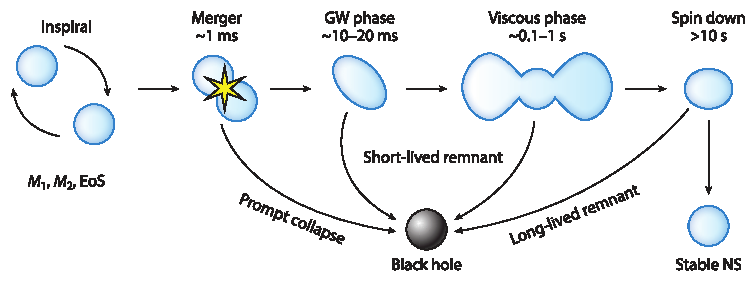
\includegraphics[width=0.70\textwidth]{Fig_3_Rad.pdf}
    \caption{
        Overview of the different phases in an \ac{NS} merger and the relative timescales. 
        The inspiral ends with the merger, when the two stars start to fuse together. 
        The early \pmerg{} evolution is entirely driven by hydrodynamics and by \ac{GW} emission. 
        If the remnant does not collapse within ${\sim}10-20\,$ms, \ac{GW} losses
        subside and other physical processes become more important: 
        Angular momentum redistribution (which is due to turbulent viscosity) 
        and neutrino losses operate over a timescale of a tenth of a second to a few
        seconds. This is also the characteristic timescale for the evolution of the remnant disk. 
        If the remnant does not collapse over a timescale of a few seconds, then it will 
        spin down because of \ac{MHD} effects over a possibly much longer timescale 
        of several seconds to a few hours. 
        (Adapted from \citet{Radice:2020ddv}).
    }
    \label{fig:intro:RadFig1}
\end{figure}


%% -----------------------------------
\section{Merger and \pmerg{}}\label{sec:intro:merg_pmerg} %ef in GRLESS
%% ------------------------------------

After \acp{NS} inspiral and merge, the dynamics of the system becomes significantly 
more complex, as temperature and density rise by orders of magnitude and new 
physical effects, \eg, magnetic fields and weak interaction, start to influence the evolution. 
The \pmerg{} phase is not well understood and mainly explored with miltiphsyics \ac{NR} 
simulations with various degrees of sophistication and resolution. 

The summary of the \ac{BNS} \pmerg{} evolution is shown in Fig.~\ref{fig:intro:RadFig1}. 
There are several trajectories that system can take, depending when/if the formed remnant 
collapses to a \ac{BH}. The early \pmerg{} phase is charaterized by strong \ac{GW} 
emission and hydrodynamic effects. After it, several interlinked processes govern the 
evolution, \eg, \ac{MHD} stresses, that contribute to the angular momentum and redistribution, 
and neutrino emission, that alters the matter composition and cools is.
If \ac{BH} does not form, the \ac{MHD} torques and residual \ac{GW} emission spin down 
the remnant.

%% ------------------------------------------------
\subsection{Dynamics and Thermodynamics Conditions} \label{sec:intro:remnant}

Prior to the merger, \acp{NS} can be considered as being in the cold, neutrino-less, 
weak equilibrium with only marginal heating due to tidal deformation at the last orbits.
The dynamics at merger is dominated by the \acp{NS} orbital motion
as $\upsilon_{rad}\ll\upsilon_{orb}$, 
%\footnote{
%    The orbital speed can be written as $\upsilon_{orb}\eqsim\Omega r\eqsim\sqrt{GM/(R_A + R_B)}$
%    that for equal mass binary is $\upsilon_{orb}/c\eqsim\sqrt{C}\eqsim0.39(C/0.15)^{1/2}$.
%    The radial velocity is beven by the evolution of the orbital frequency, as 
%    $\omega_r \eqsim 2\Omega r \dot{\Omega}/(3\Omega^2)$. The $\dot{\Omega}$ can be 
%    estimated from the fact, that orbital frequency satisfies 
%    $\dot{\Omega}_{GW}\sim(3456/125)(G\mathcal{M}/c^3)^5\Omega_{GW}^{11}$ during the 
%    inspiral. Then, the radial velocity reads 
%    \begin{equation}
%    \upsilon_r/c\eqsim\frac{192\pi}{15}\frac{G^3 M^3}{c^5(R_A + R_B)^3}\frac{q}{(1+q)^2}
%    \end{equation}
%    that for equal mass gives $\upsilon_r/c \eqsim 0.0034 (C/0.15)^3$.
%}.
%Merger time, $t_{merg}$, estimated from the \ac{GW} frequency at \acp{NS} collisition 
%for comparable \ac{NS} masses is given by 
%\begin{equation}
%    t_{merg}\eqsim\frac{1}{2f_{GW}^{contact}}\eqsim1.50\text{ms}\Big(\frac{M}{2.8\,\Msun}\Big)^{1}
%\end{equation}
%where the frequency of \acp{GW} when \acp{NS} come into contact, \ie, when the distance 
%between them, $r = R_A + R_B$ can be evaluated from the Kepler law, given by 
%the quadrupolar gravitoelectric term, % Eq.~7
%$2GM\Omega \eqsim 2(M_B/(MC_B) + M_B/(MC_B))^{-3/2}$ \cite{29},
%as 
%\begin{equation}
%    f_{GW}^{contact} \eqsim 1.327 \Big(\frac{C}{0.15}\Big)^{3/2}\Big( \frac{M}{2.8\,\Msun} \Big) \text{ kHz}
%\end{equation}
that is $\upsilon_{orb}\eqsim\Omega r\eqsim\sqrt{GM/(R_A + R_B)}$.
This indicates that 
more compact binaries experience more rapid, more violent mergers.

%%%% Remnant
%When \acp{NS} collide, their deformed cores squeeze past each other, triggering \ac{KHI},
%in the first bounce. After several of these bounces, the cores fuse into a single object.
At collision, \ac{KHI} is triggered by the \acp{NS} cores plunging into the companion,
squeezing past each other and inducing the first wave of gravity-driven compression. 
The maximum values of temperatures and densities are reached than \citep{Perego:2019adq}. 
As nuclear and centrifugal forces start to dominate, the cores bounce back until gravity 
takes over again. %This is referred to as core \bnc{}. 
%
Notably, formed in the violent, fast collision, the remnant core while is being far from 
hydrodynamic equilibrium, does not exhibit shocks. This is due to high speed of sound 
of nuclear matter at supra-nuclear densities.
%($c_s\gtrsim0.2\, c$, at $\rho\gtrsim\rho_0$)
%
Shocks, however, form at the remnant \ac{NS} surface, accelerating matter to mildly-relativistic 
velocities. %(\ref{Sec:intro:bns:ejecta}).
The fluid inside the cores remains cold 
%$T\lesssim10\,$MeV, $s\lesssim1\,k_B$/baryon 
throughout the merger, while at the interface between cores, the compression and shear 
dissipation raises the temperature to $T\sim70-110\,$MeV.
This is accompanied by the formation of the generic structure, described
by a pair of rotating hot regions, offset by $\sim\pi/2$ with 
respect to dense cold regions \citep{Kastaun:2016yaf}.
%
Overall evolution proceeds towards more axisymmetric, stable remnant, but can be 
interrupted by the \ac{BH} formation. 

%%%% Disk Foramtion
The matter outside the bouncing cores, lifted by tidal torques and squeezed out at the 
collisional interface, forms a disk (or a torus).
Due to various contributions with different properties, the disk is highly non-uniform.
The overall properties of the disk such as mass, have complex dependency on 
binary parameters, that can be expressed, at a first approximation, via fitting 
formulae to \ac{NR} simulations \citep{Radice:2017lry,Radice:2018xqa,Radice:2018ozg}. 
The generic disk evolution around the remnant consists of quasi-adiabatic expansion
of its outer layers 
%with $T^3/\rho^3\sim\text{const}$ as the \ac{EOS} is dominated by non-relativisitc baryons
and cooling of the inner regions. 
%
However, as was mentioned above, the newly born remnant is not hydrodynamically stable. 
Its dynamics is characterized by the pronounced $m=2$ bar- and $m=1$ one-armed-
deformations, \red{Refs}, inducing spiral waves, propagating through the 
disk \red{FIG}.% shocking and heating up the fluid. 
Additionally, the former leads to the strong \ac{GW} emission 
in ${\sim}10-20$~ms \pmerg{}. The backreaction from the energy and angular momentum 
loss dumps the $m=2$ mode efficiently and \ac{GW} emission subsides. 
%We refer to this evolutionary phase as \ac{GW}-dominated \pmerg{} phase.
%Notably, the $m=1$ mode, however, can persist due to mode coupling 
%\cite{Dietrich:2016phd}. 
That marks the end of the ``\ac{GW}-driven phase'' of \pmerg{} evolution. 

%%%% Disk Settling down 
Weak processes and spiral density waves cool and shock periodically the 
fluid, bringing the disk to the configuration, with an overall smooth 
temperature profile 
%from $\sim10\,$MeV at $\rho\eqsim10^{13}$\gcm to $\sim0.1\,$MeV at $\rho\eqsim10^4$\gcm
%with entropy $\in(3,10)$ $k_B$/baryon
and quasi-Keplerian orbit.
%
%%%% IF BH forms
If the remnant collapses to a \ac{BH}, the densest part of the disk is 
accreted on the dynamical timescale, reducing the total mass by half 
%and the disk maxiumum density to $\sim10^{12}\,$\gcm,
and disk shrinks \citep{Perego:2019adq}.

%%%% Magnetic fields
While \acp{MF} are not expected to affect the \ac{BNS} inspiral, their influence 
on the postmerger evolution can be strong \citep{Duez:2006qe,Kiuchi:2017zzg}, as they get amplified 
to the values exceeding that of a magnetar 
%$10^{16}\,$Gauss, 
by a variety of processes, 
\eg, flux freezing and compression, \ac{KHI} at the collisional interface \citep{Kiuchi:2015sga},
\ac{MRI}, \citep{Duez:2006qe,Kiuchi:2017zzg} and \ac{MF} winding \citep{Duez:2006qe},

Whether the ordered, large-scale \acp{MF} can form in \pmerg{} environment 
via the dynamo process is presently unknown. They are important in producing 
polar collimated outflows, jets \citep{Bucciantini:2011kx,Ruiz:2016rai} and mildly relativistic 
outflows \citep{Metzger:2018qfl,Fernandez:2018kax}. Random magnetic fields are also 
relevant for \pmerg{} evolution, as they generate stresses, enhancing angular momentum transport. 
Presently, these processes are not well understood, as seed \ac{MHD} instabilities operate at 
small scales (centimeters) and cannot be resolved in global \ac{MHD} \ac{BNS} merger 
simulations
% with reslistic initial condiitons
.
To be able to resolve the instabilities (to increase their scale), the seed \acp{MF} are 
artificially enhanced to the magnetar-strength \citep{Kiuchi:2015sga,Kiuchi:2017zzg}.
%
%%%% Alpha-viscosity model
The effect of \acp{MF} on the angular momentum transport can be approximated via 
the $\alpha$-viscosity model \citep{Shakura:1972te}. \red{More on it? For the theiry and GRLESS model?}
These effects are important 
in determining the remnant structure, lifetime and hence, the \pmerg{} \acp{GW} 
\citep{Radice:2017zta,Shibata:2017xht} 
%The timescale for the angular momentum redistribution in the remnant \cite{80} 
%\begin{equation}
%    t_{rem} \eqsim \alpha^{-1}R_{rem}^2\Omega_{rem}c_s^{-2}\eqsim 0.56\,s\Big(\frac{\alpha}{0.001}\Big)^{-1}\Big(\frac{R_{rem}}{15\,\text{km}}\Big)^2 \Big( \frac{\Omega_{rem}}{10^4\,\text{kHz}} \Big) \Big(\frac{c_s}{0.2\,c}\Big)^{-2}
%\end{equation}
%where $\Omega_{rem}$ and $c_s$ are the angular momentum and sound speed respectively.
as the loss of angular momentum brings the remnant closer to either stable, 
rigidly rotating configuration or collapse \citep{Hotokezaka:2013iia}. 
%
The \acp{MF} effects within the Keplerian disk facilitate accretion 
\citep{Fernandez:2015use,Fujibayashi:2017puw,Fernandez:2018kax,Miller:2019dpt}.
%on a timescale
%\begin{equation}
%    t_{disk} = \alpha^{-1}\Big(\frac{H}{R}\Big)^{-2}\Omega^{-1}_K \eqsim 0.78 \Big(\frac{\alpha}{0.02}\Big)^{-1}\Big(\frac{H/R}{1/3}\Big)^{-2}\Big(\frac{M_{rem}}{2.5\,\Msun}\Big)^{-1/2}\Big(\frac{R_{disk}}{100\,\text{km}}\Big)^{3/2}
%\end{equation}
%where $M_{rem}$ is the mass of the central remnant and $R_{disk}$ is the radial 
%scale of the disk.

%%%% Neutrinos
The prime cooling mechanism in the post-\ac{GW}-dominated phase is the emission of 
neutrinos, produced in the hot, dense part of the disk and remnant, and that are 
able to escape \citep{Eichler:1989ve,Rosswog:2003rv,Sekiguchi:2011zd}. 
%The typical neutrino mean free path is 
%\begin{equation}
%    \lambda_{\nu} = \Big(n_B\sigma_0(E_{\nu}/m_e c^2)^2\Big)^{-1}\simeq 24.6\,\text{m}\,(\rho/10^{14}\,\text{g}\,\text{cm}^{-3})^{-1}(E_{\nu}/10\,\text{MeV})^{-2},
%\end{equation}
%where $n_B$ is the density of baryons, and 
%\begin{equation}
%    \sigma_0 \simeq 4G_{F}^2 (m_e c^2)^2 / (\pi(\hbar c)^4)\simeq 1.76\times 10^{-44} \, \text{cm}^2
%\end{equation}
%is the typical neutrino cross section scale, and $E_{\nu}$ is the neutrino energy.
%Considering the charactersitic remnant temperature as  $T_{rem}\simeq20\,$MeV 
%energy of the thermal neutrinos then $E_{\nu}\simeq 3.15T_{rem}$ and optical depth 
%$\tau_{\nu}\simeq R_{rem}/\lambda_{\nu}=\mathcal{O}(10^{4})$.
The neutrinos are radiated on a diffusion timescale \citep{Perego:2014fma}.
%\begin{equation}
%    t_{diff} \simeq \frac{\tau_{\nu}R_{rem}}{c}\simeq 4.28\,s\Big( \frac{R_{rem}}{15\,\text{km}} \Big)^{-1}\Big(\frac{M_{rem}}{2.5\,\Msun}\Big)\Big(\frac{T_{rem}}{20\,\text{MeV}}\Big)^2.
%\end{equation}

%%%% neutrinos in the remnant and disk
Within the remnant, neutrinos are in a weak and thermal equilibrium with matter 
due to charged current reactions. There, the production of electron neutrinos, $\nu_e$,
is suppressed by degeneracy and as chemical potential $\mu_n-\mu_p+\mu_e<0$ at high temperatures, 
the electron anti-neutrinos, $\bar{\nu}_{e}$, dominate. The effect of these ``trapped'' 
neutrinos on the remnant evolution is not very strong \citep{Foucart:2015gaa,Perego:2019adq}.
%
Within the disk, however, the optical depth for neutrinos is ${\simeq}1$ so 
the they can diffuse out on a timescale of milliseconds, lowering the disk 
temperature. The cooling rate is controlled by the degeneracy state of neutrinos 
%that is kept at mild values by the feedback negative effect, higher 
%values have on the cooling rate.
\citep{Beloborodov:2008nx}.

During the early \pmerg{}, the luminosity of the electron antineutrinos 
$L_{\bar{\nu}_e} \gtrsim L_{\nu_e}$, as the 
free neutrinos are abundant in the disk and the absorption opacity for $\nu_e$ 
exceeds that of $\bar{\nu}_e$.
Thus, alongside heating and decompression, the initially cold matter in weak 
equilibrium, undergoes \textit{leptonization} 
%The heavy neutrinos, $\nu_{\mu,\tau}$, are balanced by pair processes and 
%decouple from matter at higher densities and temperatures within the remnant
%namely $\rho\gtrsim10^{13}$\gcm and $T\gtrsim8\,$MeV 
\citep{Perego:2014fma,Endrizzi:2019trv},
%The, BNS simulations including
%neutrino transport predict the mean neutrino energies at infinity
%$E_{\nu_{e}}(\sim 10\,\text{MeV})\lesssim E_{\bar{\nu}_e}(\sim 15\,\text{MeV}) \lesssim E_{\nu_{\mu,\tau}}(\sim 20\,\text{MeV})$. Notably, binaries with higher mass 
%show higher neutrino energies \cite{14,86}.
\ie, $n+\nu_e\rightarrow p + e^-$. \red{check that, from Wiki}
%
Neutrinos with different energies decouple from matter in different regions.
%due to the stron dependency of the cross section on the incoming neutrino energy.
Mildly energetic $\nu_{e}$ and $\bar{\nu}_e$ decouple at ${\sim}10^{11}\,$\gcm, found 
in the disk, while low energy neutrinos decouple at higher $\rho\sim10^{13}\,$\gcm.
The geometric surface along which neutrinos decouple is usually called ``neutrino 
surface'' \citep{Perego:2014fma,Endrizzi:2019trv}.
%The dependency of the location and the geometry of this surface on the thermodynamics 
%conditions and neutrino energy facilitates the need to coherent treatment of the 
%strong and weak interactions over a broad span of densities and temepratures.
%The energy dependent (spectral) neutrino radiation trasport is required in 
%\ac{BNS} merger simulations

%%%% Neutrino oscillations
While it has been shown that neutrino flavor conversions may occur in the \ac{BNS} 
\pmerg{} environment, \eg, the matter-neutrino oscillations, induced by the 
the fact that $\bar{\nu}_e$ decouple at smaller radii then $\nu_{e}$ 
\citep[\eg][]{Zhu:2016mwa,Tian:2017xbr}, and fast-flavor conversions above the 
neutrino surface \citep{Wu:2017drk}, their impact on the properties of the ejected 
material remains largely unexplored.
%More works of neutrino quantum kinetics equations \cite{90,91}, that include 
%collisional integral and angular and energy distributions of neutrinos are required.

%%%% EOS 
One of the main unknowns with respect to \ac{BNS} mergers, is the high density part, 
$\rho \gtrsim \rho_0$ of the \ac{NS} \ac{EOS} \citep[\eg][]{Hebeler:2013nza,Oertel:2016bki}, that relate to the 
relevant thermodynamic degrees of freedom and nucleonic interactions. For instance, 
the emergence of the new species, \eg, hyperons, pions, muons, and nuclear 
resonances, would lower the matter degeneracy, and thus, soften the \ac{EOS} \citep[\eg][]{Fore:2019wib,Vidana:2010ip}.
Additionally, the emergence of the deconfined quark matter, due to \ac{QCD} phase transition,
would alter \ac{EOS} at very high temperatures and densities,
the effect that is not well understood \citep{Busza:2018rrf}.

%% ---------------------------------------
\subsection{Fate of the Remnant}

The end product of \ac{BNS} merger depends primarily on the binary parameters, (masses, 
\mr{}) and \ac{EOS}, and in particular, on the maximum supported mass of a non-rotating 
\ac{NS}, $M_{max}^{TOV}$ \citep{Shibata:2016}, as well as on the finite temperature and 
non-beta-equilibrium composition effects. 
%
The \ac{BH} formation directly at merger is usually referred to as \ac{PC}. 
The conditions for it depend  are not well understood. 
Simulations show that in equal mass binaries, \ac{PC} occurs if the total mass 
$M\gtrsim M_{thr} = k_{thr}M_{max}^{TOV}$, where $k_{thr}\in(1.3,\,1.7)$ that depends on 
\ac{EOS} \citep{Shibata:2005ss,Shibata:2006nm,Hotokezaka:2011dh,Bauswein:2013jpa}.
%(or $\kappa_2^T\lesssim43-73$, or $\tilde{\Lambda}\lesssim338-386$.
Simulations of unequal mass binaries show that the threshold is lower \citep{Bauswein:2017vtn}, 
and $k_{thr}\propto C_{1.6}$, with $C_{1.6}$ being the compactness of the $1.6\,\Msun$ 
\ac{NS} \citep{Hotokezaka:2011dh,Bauswein:2013jpa,Bauswein:2017vtn}. 
%As \ac{PC} cases are 
%not expected to ejecta large amount of material and be \ac{EM}-loud (in case of 
%comparable mass binary), the \GW{} is believed to be not a \ac{PC} case, 
%\cite{Margalit:2017dij,Bauswein:2017vtn}. 

A remnant that does not undergo \ac{PC} is a massive \ac{NS}, temporarily supported 
by fast rotation \citep{Baumgarte:1999cq,Rosswog:2001fh,Shibata:2005ss,Shibata:2006nm,
    Sekiguchi:2011zd,Hotokezaka:2013iia,Bernuzzi:2015opx}, whose lifetime depends 
intricately on the \ac{EOS}, finite temperature effects, and viscosity. A commonly 
adopted classification, based on the properties of equilibrium models (neglecting the 
dynamical, finite temperature, and magnetic effects), \ie, $M_{max}^{TOV}$ and
$M_{max}^{RNS}$\footnote{
    $M_{max}^{RNS}$ is the maximum mass of a rigidly rotating \ac{NS} (no differential 
    rotation) supported by zero-temperature (cold) \ac{EOS}. Also sometimes referred as 
    mass-shedding limit.
    % $M_{max}^{TOV}$ and $M_{max}^{RNS}$ are agnostic to thermal or magnetic eects 
    %which can impact the stability of the remnant in nontrivial ways (108, 72)
}
distinguishes between 
\ac{HMNS} if $M{>}M_{max}^{RNS}$, 
\ac{SMNS} if $M_{max}^{TOV} {\leq} M_{max}^{RNS}$,
and stable \ac{MNS} if $M {<} M_{max}^{TOV}$ \citep[\eg][]{Baumgarte:1999cq}.
A \ac{HMNS} is supported by differential rotation that viscosity reduces with time. 
Hence, it is expected to collapse to a \ac{BH}. A \ac{SMNS} can avoid the collapse 
even after reaching rigidly rotating configuration. The lifetime of a \ac{HMNS} and 
a \ac{SMNS} depends on the efficiency of mass and angular momentum loss 
(to, \eg, \acp{GW} and massive winds) and finite temperature effects \citep{Radice:2018xqa}. 
%
Discussing the \ac{NR} simulations we shall distinguish between \textit{short-lived} remnants, 
that collapse to \ac{BH} during \ac{GW}-dominated phase, 
% taht correspods to ${\sim}10-20\,$ms after merger \cite{107,60}
and \textit{long-lived} otherwise.

If a remnant can achieve rigid rotation, its evolution then is characterized by the emission 
of \acp{GW} (due to residual asphericity) and magnetic braking, reducing further its 
angular momentum, until either a \ac{BH} forms, or a stable non-rotating equilibrium is reached.
The observations of \acp{SGRB} with X-ray plateu 
\citep{Zhang:2000wx,Lasky:2015lej,Fan:2013cra}, if indeed given by the 
magnetar activity\footnote{
    There are other possible explanations behind the X-ray plateu emission of \acp{SGRB} 
    \citep{Oganesyan:2019jij}
}, suggest that the remnant may survive from seconds to hours \citep{Fan:2013cra,Ravi:2014gxa}.
Most of the energy, ${\sim}10^{52}\,$erg, that a remnant needs to lose before collapsing 
most likely is carried away in form of \acp{GW}, as \ac{EM} observations of \GW{} suggest.
%This emission can be observed for the nearby event \cite{111}, priding direct information 
%on the remnant fate. However this emission was not observed for \GW{} \cite{67,68}

From \ac{EM} observations of the merger the fate of the remnant, albeit in the 
model-dependent way can be inferred. In case of \GW{}, the presence of such counterpart 
strongly disfavors \ac{PC} (as those are not expected to eject any significant amount 
of matter) \citep{Margalit:2017dij,Bauswein:2017vtn,Radice:2017lry}, while leaving 
the question whether it was \ac{HMNS} or \ac{SMNS} open. \citet{Margalit:2017dij} suggested 
that the remnant was short-lived, on account of the non-detection of the expected ${\sim}10^{52}\,$erg, 
from the spin-down of the long-lived one. Assuming thus that \GW{} produced a \ac{HMNS}, 
allows to put a constraint $M_{max}^{TOV}{\lesssim}2.2\Msun$ \citep{Margalit:2017dij}.
%
On the other hand, if the magnetar model of \acp{SGRB} is applied to \GW{} 
\citep{Ai:2018jtv,Li:2018hzy,Piro:2018bpl}, the remnant is required to be long-lived
(${\sim}$months) and exhibit weak dipol \acp{MF} \citep{Ai:2018jtv}, leading to a different 
constraint on the maximum mass of the non-rotating star, $M_{max}^{TOV}{\gtrsim}2.2\Msun$ 
%and up to an order of magnitude lower ejecta mass ${\sim}10^{-3}\,\Msun$, that is attributed 
%to reducied amount of emergy from radioactive decay is required to explain the observed 
%UV/optical/infrared observations \cite{16}. 
%There have been indications of the X-ray flaring activity in \GRB{} \cite{117}, but 
%follow-up observations did not confirm it \cite{118}
. 



%% --------------------------------------------------------------------------
%%               N U C L E O S Y N T H E S I S
%% --------------------------------------------------------------------------

\section{Ejecta, \nuc{}, electromagnetic counterparts}

\subsection{$R$-process \nuc{}} \label{sec:intro:nucleo}

Nuclides with atomic number  $A{\geq}56$ cannot be synthesized via nuclear burning 
due to their large Coulomb barriers and are produced via 
neutron capture processes \citep{Burbidge:1957}.
% Nucleosynthesis Cites
The maximum $A$ of a nuclide is limited by its binding energy, $Q_n$. 
At $Q_n{\simeq1}$~MeV photodisintegration starts breaking nuclides apart. 
The place in the parameter space of temperature and density where this occurs 
is called \textit{neutron drip line} \citep{Rolfs:1988}.
% Fast and Slow
Nuclides produced via neutron capture are generally unstable to $\beta$-decay,
and depending on whether the timescale for the decay is slower (faster) than 
the timescale of neutron capture, one distinguish rapid (slow) process called,
\rproc{} (\sproc{}).
%
The \sproc{} moves along the valey of stability, while \rproc{} moves along the 
neutron drip line.
%
When a nuclide reaches a closed neutron shell configuration, the cross-section 
for the subsequent neutron capture shrinks, and capture processes suspends until 
several $\beta$-decays take place. This results in the overproduction of nuclides 
that are located at the intersection between the neutron drip line and closed 
neutron shell for the \rproc{}. This manifests as ``peaks'' in the final abundance 
pattern at $A$ corresponding to these configurations.
Closed shell nuclides are located at $N=50,\: 82, \: 126$ and 
corresponding abundance peaks $A=80,\:130,\:194$ for \rproc{} 
(see \eg, \citet{Arnould:2007gh})

%%%% R-proces cites
Conditions for the \rproc{} can be achieved in different astophysical cites, \eg, 
certain types of \acp{SN} and \ac{BNS} mergers where very neutron rich (low 
electron fraction, $Y_e$) conditions can be reached
\citep{Mathews:1990,Thielemann:2011,Lippuner:2015gwa,Siegel:2019mlp}. 
Regaring \acp{SN}, the wind driven by the neutrino flux from the hot, deleptonized
core \citep{Qian:1996xt} is suggested as a promising cite \citep{Woosley:2002,Wanajo:2006mq}.
However, high $Y_e$ found in such winds do not allow for the full \rproc{} and only ``light'' heavy 
nuclide, up to $A\sim130$, can be synthesized 
\citep{Qian:1996xt,Thompson:2001ys,Fischer:2010,Roberts:2010,MartinezPinedo:2012rb,Wanajo:2013} 
%
A full \rproc{} can be achieved in so-called magnetorotationally driven \ac{CCSN},
(a rare type of \ac{CCSN} with a rapidly spinning strongly magnetized core), 
initiated by the \ac{MRI} and accompanied by a % magnetorotational processes \eg, 
formation of a 
collimated bipolar jet 
\citep{Wheeler:2000,Akiyama:2003,Burrows:2007yx,Mosta:2014jaa,Mosta:2015,Siegel:2019mlp}.
Conditions within such a jet were found to be suffient for full \rproc{} \nuc{} 
\citep{Winteler:2012,Nishimura:2015nca}.
%The rarity of this type of \acp{SN}, 
%however, might not allow for them to be the dominant source or \rproc{} material 
%\citep{Nishimura:2015nca} 

Neutron-rich ejecta from \ac{BNS} and \ac{NSBH} mergers are regarded as one of 
the main cites or \rproc{} \nuc{}.
%
%Mergers of two \acp{NS} or a \ac{NS} and a \ac{BH} are regarded as one of the main cites 
%of \rproc{} material.% (See Sec.~\ref{sec:intro:bns_merg}). 

%%%% Fission cycling
Under the very neutron-rich conditions, 
the nuclides beyond $A=300$ can be produced. Being unstable to fission, they 
decay into seed nuclides softly after formation.
However, before they reach the valley of stability, neutron captures occurs again, and the cycle repeats.
This is so-called \textit{fission cycle}.
It is maintained as long as there are free neutrons, after which nuclides decay 
for the last time, forming a remarkably robust abundance pattern independent of the 
number of cycles (and thus on the exact conditions) 
(see Figure 4 in \citet{Korobkin:2012uy}).

%%%% Cites
There is no consensus yet on what is the main source of \rproc{} material in the 
Universe. 
Observed \rproc{} abundances in \ac{MP} stars, formed early in the Galactic history, 
point towards a sources that was active in the early Universe, which is in tension with the long, 
$10^{6} - 10^{9}$ years, delay time required for compact object inspiral 
\citep{DeDonder:2004cx,Dominik:2012kk}. This estimate, however, depends strongly on the 
uncertain common envelop evolution phase of the massive binary (progenitors)
\citep[\eg][]{Dominik:2012kk}.
%
Observations of \acp{UFG} suggest that the stars there have been enrighed by rare, 
high-yield events (as \ac{UFG} Reticulum II showed abundances simialr to solar, 
while other \ac{UFG} galaxies show $2-3$ times lower abundances) \citep{Ji:2016}.
%
Earth crust and meteorites $^{244}$Pu studies also point towards rare, high-yield 
events \citep{Wallner:2015,Tsujimoto:2017}. This scenario has been confirmed with 
models of galactic mixing \citep{Hotokezaka:2015zea}.
%
It is however difficult to explain the observed uniform distribution of \rproc{} 
elements in the Galaxy with such events \citep{Argast:2003he}.
%
Population synthesis models have indicated that with a contribution from 
magnetorotationallydriven \acp{CCSN} the compact object mergers can account for the 
observed distribution \citep{Ishimaru:2015,Cescutti:2015,Wehmeyer:2015,VanDeVoort:2015}.



%% ----------------------------------
\subsection{Kilonova} \label{sec:intro:kilonova}

%The \rproc{} \nuc{} in ejecta is primarily determined by the electron fraction 
%\citep{Lippuner:2015gwa}, $Y_e$, producing $3$rd ($1$st) elements of the \rproc{} peaks 
%%(See Sec.~\ref{sec:intro:nucleo}) 
%if the $Y_e\gtrsim 0.3$ ($Y_e \lesssim 0.2$) 
%with respective abundances in the former remarkably close to solar. 
%%The transition at $Y_e{\simeq}0.25$ is rather sharp.

\citet{Li:1998bw} suggested that 
radioactive decay of the material enriched with \rproc{} elements,
ejected in \ac{BNS} or \ac{NSBH} mergers,
can power the \ac{EM} transient.
%
Authors showed that contrary to the normal \acp{SN}, 
the ejecta would quickly become transparent to its own emission, peaking on a timescale 
of around a few days. 
%
The main difficulty in this pioneering work was the lack of a \nuc{}
model to model to estimate the radioactive heating of the ejecta. 
%
The understanding of \ac{kN} has significantly improved since then
\citep[\eg][]{Kulkarni:2005jw,Metzger:2010,Roberts:2011,Metzger:2016pju,Wollaeger:2017ahm} 
and advanced even further with the detection of \AT{} \citep[\eg][]{Metzger:2019zeh}.


%% --------------------------
%% M O D E L L I N G  K I L O N O V A
%% --------------------------

The way to model \ac{EM} emission from the stratified, asymmetric ejecta is to perform 
multi-dimensional, multi-group radiative transfer simulation coupled to \ac{HD} (or \ac{MHD}) 
simulation of the ejecta itself \cite[\eg][]{Bulla:2019muo}.
%
It is however possible to compute the bolometric properties considering the total amount 
of energy released and emitted by radioactive decay within ejecta. 

%
%Here a simplified model is considered of a transient, powered by the radioactive decay 
%within the ejecta only. Several other assumptions are made. In particular, the ejecta 
%expansion is homologous (faster matter ahead of slow one) \citep{Rosswog:2013kqa}. %%{(Rosswog et al 2014)}
%
%\red{this is based on the Barnes PhD thesis on Opacities for Kilonva (Rad.Transport)}
%\red{Based on Metzger paper }

%% --------------------------
%% SIMPLE MODEL
%% --------------------------

%\subsubsection{Basic ingredients}

%Consider the following simplified approach to compute the \ac{EM} signal from \rproc{}
%elements enriched material. 
Let the radioactive decay of a newly synthesized heavy isotope, $i$, release 
$\dot{Q}_i \propto \exp(-t/\tau_i)$ energy, with $\tau_i$ being its half-life.
Then, assuming equal distribution of $\tau_i$ per logarithmic time
%(at any $t$ the dominant species have $\tau\sim t$), 
the heating rate of the ejecta at time $t$ is 
$\dot{Q}_{LP} = f M c^2 / t$,
where $f$ is free parameter and $M$ is the ejecta mass
\footnote{
    In general heating is time-dependent as thermodynamic histories of the expanding 
    ejecta (from \ac{NR} simulations) showed \citep{Metzger:2010,Roberts:2011,Korobkin:2012uy}.
    See also \citet{Hotokezaka:2017dbk} for the discussion on physical principles behind the decay.
}.
%
%In addition, provided by \citet{Li:1998bw}, normalization $f$ resulted in overestimation of the peak 
%luminosity of the \ac{kN}, that plagued the \ac{kN} searches for a decade 
%\cite{Rosswog:2005su,Dong:2015oea,Bloom:2005qx,Kocevski:2009gv}. 

The first self-consistent estimation of the heating rates based on the \ac{NRN} 
calculations of the \rproc{} in the ejecta, carried out by the \citet{Metzger:2010}. 
The authors showed based only on dynamical ejecta, the \ac{EM} transient is ${\sim}10^3$ 
times brighter then Novae -- hence, the term, kilonova was coined. 
%
%It was also shown the ejecta electron fraction does not affect the heating rates
%considerably, and performed the first estimations of the thermalization 
%efficiency of decay products.
%
%The term macronova was however coind by \citet{Kulkarni:2005jw} who considered a 
%transient powered by the decay of radioactive $^{56}$Ni and free neutrons. 
%However, as it was shown later, $^{56}$Ni can only be formed in small quantities on 
%the outskirts of the ejecta.

The calculation of observed \ac{EM} emission is complicated by the %ejecta opacity, 
%as there is a 
general lack of experimental data and numerical models of the singly 
and doubly ionized heavy \rproc{} elements opacities. 
Simple iron-group gray opacities, first employed for this issue \citep{Roberts:2011}, 
were shown to severely underestimate those of lanthanides and actinides with their 
complex atomic atomic structures (given by open $f$-shells) 
\citep{Kasen:2013xka,Tanaka:2013ana}. 
%
Higher opacities shift light curve peak time by ${\sim}1$~weak \citep{Barnes:2013wka} 
and shift the spectral peak from optical/\ac{UV} to \ac{NIR}.

%% ----------------------------------------
%\subsection{Basic model of the \ac{kN}}
%% ----------------------------------------

For a single shell of hot and optically thick matter 
(that tjhe thermal energy is not immediately radiated away), 
expanding with constant velocity, $\upsilon$, 
%such that $R\approx\upsilon t$ at any point in time $t$, 
the radiation diffusion timescale is given by 
%
\begin{equation}
\tau = \rho \kappa R = \frac{3}{4}\frac{M\kappa}{4\pi R^2}, \hspace{5mm} 
t_{diff} \approx \frac{R}{c}\tau = \frac{3}{4}\frac{M\kappa}{4\pi c R} = \frac{3}{4}\frac{M\kappa}{\pi c \upsilon t}
\end{equation}
%
where $M$ is the ejecta mass, $\kappa$ is the opacity (cross section per unit mass), 
$\rho$ is the density, \eg, $\rho=3M/(4\pi R^3)$ is the mean density.
%
As ejecta expands and cools (via adiabatic losses) its opacities decreases, 
and so does the diffusion timescale. 
When $t_{diff}$ reaches $t$, the radiation can escape the ejecta \citep{Arnett:1982}. 
Hence, the characteristic timescale of the peak of emitted radiation 
%
\red{check the eq.}
\begin{equation}
t_{peak} = \Big(\frac{3}{4}\frac{1}{\beta}\frac{M\kappa}{\pi \upsilon c}\Big)^{1/2}
\end{equation}
%
where the constant $\beta$ depends on the exact density profile of the ejecta. 
The $t_{peak}$ is of order of days for lanthanides-free and weeks for lanthanides-rich ejecta.
The peak luminosity is set by the total heating rate $\dot{Q}(t)$ within the ejecta, 
as described by the \textit{Arnett's Law} \citep{Arnett:1982}. 

%% ----------------------------------------
%\subsubsection{Emission from stratified ejecta}
%% ----------------------------------------

%Consider the ejecta with a given mass-velocity distribution, that can be approximated 
%as $M_{\upsilon} = M(\upsilon / \upsilon_0)^{-\beta}$, for $\upsilon \geq \upsilon_0$,
%where $M$ is the total mass, $\upsilon_0$ is the average, minimum velocity. 
%The parameter $\beta$ can be set to $3$ \citep{Bauswein:2013yna}. %%{(Bauswein et al 2013a)}. 
%However see \citet{Piran:2012wd}%%{Piran et al 2013} 
%for a more complex velocity profiles.
%%
%%
%The diffusion timescale defines when the radiation escapes the ejecta. For a layer with 
%$\upsilon$ and $M_{\upsilon}$ and opacity $\kappa_{\upsilon}$ it is 
%%
%\begin{equation}
%t_{d,\upsilon} \approx \frac{3}{4\pi}\frac{M_{\upsilon}\kappa_{\upsilon}}{\beta Rc} = 
%\frac{1}{4\pi}\frac{M_{\upsilon}^{4/3}\kappa_{\upsilon}}{M^{1/3}\upsilon_0 t c}
%\end{equation}
%%
%where $\beta=3$ was assumed. 
%%
%This equation implies that at time $t=t_{d,\upsilon}$ the radiation from the layer 
%$M_{\upsilon}$ peaks.
%%
%The $M_{\upsilon}(t)$ is related to the total mass of the ejecta and 
%peak time (when radiation diffuses from the entire ejecta)
%%
%\begin{equation}
%M_{\upsilon}(t) = 
%\begin{cases}
%M(t/t_{peak})^{3/2},& t<t_{peak}, \\
%M, &t>t_{peak}
%\end{cases}
%\end{equation}
%%
%where $t_{peak} = (3M\kappa / (4\pi \beta \upsilon c))^{1/2}$ with 
%$\upsilon = \upsilon_0$. \red{Did not understand}
%%
%Outer layers with $M_{\upsilon} < M$ peak first, while the deepest layers peak later but 
%set the luminosity of the whole ejecta (assuming that the the opacity is constant in the 
%ejecta. 
%%
%The radial evolution of each layer $M_{\upsilon}$ of mass $dM_{\upsilon}$ is given by 
%%
%\begin{equation}
%\frac{dR}{dt} = \upsilon,
%\end{equation}
%%
%and the layer's thermal energy changes according to 
%%
%\begin{equation}
%\label{eq:theory:mkn:energ}
%\frac{dE_{\upsilon}}{dt} = \underbracket{-\frac{E_{\upsilon}}{R_{\upsilon}} 
%    \frac{dR_{\upsilon}}{dt}}_{PdV\text{ losses}} - 
%\underbracket{L_{\upsilon}}_{\text{rad. los.}} + \underbrace{\dot{Q}}_{\text{heating sources}},
%\end{equation}
%%
%where the radiative losses take form
%%
%\begin{equation}
%L_{\upsilon} = \frac{E_{\upsilon}}{t_{d,\upsilon} + t_{lc,\upsilon}},
%\end{equation}
%%
%in which the $t_{lc,\upsilon} = R_{\upsilon}/c$ limits the energy loss to the 
%light crossing time (important for when the layer is optically thin) \red{did not understand}.
%%
%The heating sources $\dot{Q}$ include
%%
%\begin{equation}
%\dot{Q}(t) = \underbrace{\dot{Q}_{r,\upsilon}}_{\text{radioactivity}} + \underbrace{\dot{Q}_{mag}}_{\text{magnetar}} + 
%\underbrace{\dot{Q}_{fb}}_{\text{fall-bak accretion}}.
%\end{equation}
%%
%%
%Next, even though in principle the effect of radiation pressure on ejecta oughtto 
%be considered, in case where radioactive heating, total energy input 
%$\int \dot{Q}_{r,\upsilon}dt < E_{kin,0}$ of the ejecta \citep{Metzger:2010,Rosswog:2013kqa} 
%%\cite{(Metzger et al 2011; Rosswog et al 2013)}, 
%this effect can be neglected.
%Meanwhile, central engine might provide enough energy to modify the free expansion 
%model. Then the equation for the central shell velocity evolution reads 
%%
%\begin{equation}
%\label{eq:theory:mkn:velcenteng}
%\frac{d}{dt}\Bigg(\frac{M\upsilon_0^2}{2}\Bigg) = M\upsilon_0\frac{d\upsilon_0}{dt} = \frac{E_{\upsilon_0}}{R_0}\frac{dR_0}{dt}
%\end{equation}
%%
%Here, the term with $E_{\upsilon_0}$ balances the $PdV$-\textit{loss} term in the 
%thermal energy equation (for $dE_{\upsilon}/dt$)
%%
%To compute the emitted radiation, first assume the black-body emission, 
%the thermal emission, with effective temperature 
%%
%\begin{equation}
%T_{eff} = \Bigg(\frac{L_{tot}}{4 \pi \sigma R_{ph}^2}\Bigg)^{1/4}
%\end{equation}
%%
%where $L_{tot} = \sum(L_{\upsilon dm_{\upsilon}})$ is the total luminosity 
%(cumulative for all mass shells). At the point where optical depth 
%$\sum(\kappa_{\upsilon}dm_{\upsilon})=1$ the photosphere is located with 
%radius $R_{ph}(t)$. 
%%
%%The flux density of the source at photon frequency $\nu$ is given by 
%%%
%%\begin{equation}
%%F_{\nu}(t) = \frac{2\pi h \nu^3}{c^2} \frac{1}{\exp\Big(\frac{h\nu}{kT_{eff}}\Big) - 1} \frac{R_{ph}^2}{D^2}
%%\end{equation}
%%%
%%where, $D$ is the distnace to the source. (Cosmological effects are neglected here).
%%
%Additionally, the opacity $\kappa_{\upsilon}$ depends on the temperature of the 
%layer $T_{\upsilon}$, that itself can be computed as 
%%
%\begin{equation}
%T_{\upsilon} = \Bigg(\frac{3E_{\upsilon}}{4\pi a R^{3}_{\upsilon}}\Bigg)^{1/4}
%\end{equation}
%%
%assuming that the ejecta internal energy is dominated by the radiation. 
%%
%%
%Finally, in order to compute the \ac{EM} emission from the ejecta, 
%the equation Eq.~\eqref{eq:theory:mkn:energ} ought be solved for $E_{\upsilon}$ 
%(and $L_{\upsilon}$) for every shell with $dM_{\upsilon}$ and $\upsilon>\upsilon_0$. 
%%
%The velocity distribution can be assumed fixed 
%(\eg $M_{\upsilon} = M(\upsilon/\upsilon_0)^{-\beta}$,  
%if only the internal heating are important. If however, the central engine energy 
%input is important, the the velocity of the central layer evolves according to
%Eq.~\eqref{eq:theory:mkn:velcenteng}.
%%
%Initial kinetic energy of the ejecta is quickly removed by the adiabatic expansion 
%and the thermal energy of the ejecta, when its emission peaks, is dominated by the heating.

%% -----------------
%% \paragraph{Opacity}
%% -----------------

In this simplified description thee key components can be identified for modeling the \ac{kN}.
These are 
%\begin{itemize}
    %\item
    (i) ejecta geometry and properties, $M$, $\upsilon$, $Y_e$; 
    %\item 
    (ii) composition of the expanding ejecta and its optical opacity; 
    %\item 
    (iii) dominant sources of energy within the ejecta, heating rate $\dot{Q}(t)$, and how 
    efficient this energy thermalizes.
%\end{itemize}
%
%We discuss the properties of the ejecta from \ac{BNS} mergers in the chapter~\ref{ch:bns_sims}.
%Here we focus on two other ingredients.

Regarding opacity, there are several sources of opacity that affect photons with
different energies that include 
%%%% --- free-free opacities
%For the photons of the lowest energy (frequency), \ac{FIR}, the free-free absorption 
%in the ionized gas is the dominant source of opacity. Expansion, the recombination removes 
%free $e$, also decreases $\rho$, and thus $\kappa_{ff}$.
(i) free-free transitions, especially in lanthanides and actinides with their 
valence, partially filled $f$-shell, affecting photons of lowest energies, in \ac{FIR} band; 
%%%% --- bound-bound opacities
%For \ac{NIR}/optical photons, the bound-bound transitions are the main source of opacity. 
%Here the dependency on the ejecta composition strongly affects the \textit{effective} 
%continuum opacity. If most complex atoms in the ejecta belong to the iron group, with 
%valence $d$-shell electrons, then the opacity is moderate. However, if elements with 
%valence, partially filled $f$-shell, (lanthinides \& actinides), are present, then the 
%opacity increases by up to two orders of magnitude
%\citep{Kasen:2013xka,Tanaka:2013ana,Fontes:2015,Fontes:2017zfb}. 
%Bound-bound opacity rises with photon $\nu$ (as the number of lines).
%
%The \textit{plank mean expansion opacity} can be approximated as 
%$\kappa_r = 200 (T/4000K)^{5.5}$ cm$^2$g$^{-1}$ for $T\in(1-4)\times10^3$~K and just 
%$\kappa_r = 200$ cm$^2$g$^{-1}$ for $T\in(4-10)\times10^{3}$~k, motivated by 
%Figure~10 it \citet{Kasen:2013xka}. More accurate opacity estimations are plagued by the 
%complexity of the atomic structure. The quantum mechanics models of high-$Z$ atoms exists, 
%but has to be calibrated to the so far absent experimental data.
(ii) bound-bound transitions, that are the main source of opacities for 
\ac{NIR}/optical photons, 
%%%% --- Line opacity -> Effectve continoum opacity
%Additional complexity arises in approximation the line opacities to the effective opacity.
%One common way is to consider the line expansion opacity formalism \citep{Pinto:2000}, that is 
%based on the Sobolev approximation. This method was applied to \acp{kN} modeling by 
%\citet{Barnes:2013wka} and \citet{Tanaka:2013ana}. However, it is unreliable if line width is 
%large \ie, if line spacing of strong lines become comparable to the intrinsic thermal line width 
%\citep{Kasen:2013xka,Fontes:2015,Fontes:2017zfb}. 
(iii) specific optically thick lines, 
%%%% --- clumping
%In addition, clumping that might occur when $T\leq10^3$~K might affect escaping 
%emission \citep{Takami:2014oqa}. The formation of the ``\rproc{} dust'' may have a complex 
%effect on optical/\ac{UV} opacity. The process of dust formation is complex and not 
%well understood in general \citep{Cherchneff:2009sj,Lazzati:2016}
(iv) ejecta clumping, 
%%%% --- Ejecta re-ionisation
%For higher energy photos, \ac{UV}/X-ray, bound-free transitions dominate the opacity. 
%For that ejecta ought to become mostly neutral, which occures naturally as it cools, unless 
%there is a source of ionizing radiation, \eg, the remnant. 
%See for details in \eg, \citet{Metzger:2013cha}. 
%Even though very large luminocities are required from the engine initially, 
%they decrease rapidly as ejecta expands. Thus, at late times it is possible that ejecta would be 
%re-ionized, especially in case of a long-lived remnant \citep{Metzger:2013cha}. The re-ionisation 
%can reduce the optical opacity, reducing the prominence of \ac{FIR} peak, 
%a generally regarded distingushed feature of a Kilonova.
(v) ejecta re-ionisation by \eg, high energy photons from the central engine.
%%%% --- X-ray,. Gamma-rays, thermalization
%At even higher energies, hard X-ray photons, an important source of opacity is the 
%electron scattering with Klein-Nishina corrections. Notably, if the wavelength of photons 
%become smaller then the scale of an atom, the contribution from both, free and bound into 
%nuclei electrons ought to be considered. At high energies, the scattering of photons is inelastic. 
%However, these processes are important as ejecta opacity to very high energy photons, 
%$\gamma$-rays with energy in order of MeVs, determines the thermalisation of the \rproc{} 
%decay products.
%%
%%% pair-creation
%For extremely high photon energies $h\nu \gg m_e c^2$a pair creation becomes important. 
%In particular this is so if remnant is a magnetar with large spin-down luminosity. 
%Then, the at peak of the \ac{kN} emission, the pair creation might prevent pair-creation 
%photons from escaping the kilonova. 

%The calculation of opacities is complicated by the fact that the 
%Additional complexity arises in approximation the line opacities to the effective opacity.

%%%% --- compliecations in calculations 
An additional complication in opacity calculation arises from the fact that the ejecta 
is rapidly expanding, which implies that the matter ``sees'' incoming radiation as 
Doppler shifted. 
One common approach is to consider \textit{plank mean expansion opacity}, 
\red{in MKN it is mean plank opacities}
%that for 
%$\kappa_r = 200 (T/4000K)^{5.5}$ cm$^2$g$^{-1}$ for $T\in(1-4)\times10^3$~K and just 
%$\kappa_r = 200$ cm$^2$g$^{-1}$ for $T\in(4-10)\times10^{3}$~k, motivated by 
%Figure~10 it \citet{Kasen:2013xka}.
calculation of which, however, still requires complex atomic calculations.
%
The Sobolev approximation is commonly used in the line expansion opacity formalism 
\citep{Pinto:2000}.
This method was applied to \acp{kN} modeling by \citet{Barnes:2013wka} and \citet{Tanaka:2013ana}. 
However, it is unreliable if line width is large \ie, if line spacing of strong 
lines become comparable to the intrinsic thermal line width 
\citep{Kasen:2013xka,Fontes:2015,Fontes:2017zfb}. 


%% ----------------------------
%% \paragraph{\rproc{} heating}
%% ----------------------------

The main source of energy in expanding ejecta shell of mass, $dM_{\upsilon}$,
and velocity, $\upsilon$, that has a fraction of \rproc{} elements, $X{r,\upsilon}$, 
is given by the specific heating, $\dot{e}_r(t)$, and can be approximated as 
%
\begin{equation}
\dot{Q}_{r,\upsilon} = dM_{\upsilon}X_{r,\upsilon}\dot{e}_{r}(t).
\end{equation}
%
The heating occurs through a combination of $\beta$- and $\alpha$-decays, 
and fission \citep{Metzger:2010,Barnes:2016umi,Hotokezaka:2017dbk}. 
The decay products then thermalize with an efficiency, $\varepsilon_{th,\upsilon}$, 
that depends on interactions between them and thermal plasma. 
Neutrinos can freely escape the ejecta. Very high energy photos, gamma rays, 
are also free after about ${\sim}1$~day as the Klein-Nishina opacity decreases 
\citep{Hotokezaka:2017dbk,Barnes:2016umi}.
%
The $\alpha$ and $\beta$ particles however interact efficiently with the matter via 
ionization \citep{Barnes:2016umi} and Coulumb scattering \citep{Metzger:2010}.
%\red{Here it repeats the Barns et al findings on thermalization efficiency}
For a fixed energy $\alpha$-particles thermalize more efficiently, then 
$\beta$-particles. For charged particles, the process depends on the magnetic 
field strength and configuration \citep{Barnes:2016umi}. 
%
Additionally, if actinides are produced in \rproc{}, their decay, 
involving $\alpha$-particles allows for higher thermalization efficiency. 
%\red{double check with before, Barnes}. 
Thus, nuclear phsyics input, that determines the amount of actinides, 
have an effect on the thermalization efficiency of \rproc{} elements in the ejecta
\citep{Barnes:2020nfi}.
%
%For a neutron-rich ejecta, $Y_e\leq0.2$, the heating rate is dominated by a large statistical 
%ensemble of nuclei, and the following can be assumed \citep{Korobkin:2012uy},
%%
%\begin{equation}
%\dot{e}_r = 4\times 10^{18} \varepsilon_{th,\upsilon}(0.5 - \pi^{-1} \arctan[(t-t_0)/\sigma])^{1.3} \text{ erg } \text{s}^{-1} \text{g}^{-1}
%\label{eq:kilonova:heat_korob}
%\end{equation}
%%
%Here $t_0=1.3$~s, $\sigma=0.11$~s constants. 
%The $\varepsilon_{th,m}$ is the thermalisation efficiency.
%In general, both $\varepsilon_{th,\upsilon}$ and 
%%
%The heating rate prescribed by this equation has first a constant segment, $\propto1$~s, 
%(depletion of free neutrons by $r$-process) and a decrease segment $\propto t^{-1.3}$, 
%(when heavy nuclei decay to stability) \citep{Metzger:2010,Roberts:2011}. 
%Notably, at higher $Y_e$, the nuclear heating is dominated by specific nuclei and has a complex form.
%%
%It was shown however, that on a timescale relevant for \ac{kN}, and $Y_e$ present in \ac{BNS} 
%($Y_e\leq0.4$), the heating rate can be assumed constant within the accuracy of a few.
%(see \eg, Fig.~7 in \citet{Lippuner:2015gwa}).
%%
%The dependency of $\dot{Q}_{r.\upsilon}$ on the nuclear physics models was shown to be week, 
%unlike the $r$-process abundances themselves \citep{Eichler:2014kma,Wu:2016pnw,Mumpower:2015ova}.
%See however \citet{Barnes:2020nfi} for a more recent assessment.
%
%Regarding the thermalization efficiency of the energy released, \citep{Barnes:2016umi} provides 
%a recipe that sets the $\varepsilon_{th,\upsilon}$ decreasing from $\sim0.5$ at around 
%$1$~day to $\sim0.1$ at around $1$~week. 
%
%\begin{equation}
%\varepsilon_{th,\upsilon}(t) = 0.36 \Bigg[ \exp(-a_{\upsilon}, t_{day}) + \frac{\ln(1+2b_{\upsilon} 
%    t_{day}^{d_{\upsilon}})}{2b_{\upsilon}t_{day}^{d_{\upsilon}}} \Bigg]
%\end{equation}
%
%where $t_{day}$ is the time in days, ${a_{\upsilon}, b_{\upsilon}, d_{\upsilon}}$ are the constants that 
%depend on the ejecta layer properties, mass and velocity. 

%%%% -------------------------------
%\subsection{\ac{kN} properties}
%%%% -------------------------------
%
%From a simple, toy model \citep{Metzger:2016pju}, the ejecta properties can be translated 
%into the properties of light curves. 
%%
%Consider the case where the lanthanides-rich ejecta is present, \eg, in tidal outflows of 
%\ac{BNS} and \ac{NSBH} mergers. There a toy model predicts a light curve from such low-$Y_e$ 
%ejecta that peaks in \ac{NIR} (in relatively good agreement with radiation transport model of 
%\citet{Barnes:2016umi}) on a timescale of several days (week). This is so-called ``red \ac{kN}''.
%The disagreement with radiation transfer models most noticeable in the post-peak period, 
%where toy model predicts sharp decay, while the radiation transport models predict smooth decline. 
%The reason for it is the toy model's assumption of optically thick black-body emission. 
%As ejecta expands cools and become optically thin, this assumption breaks down.
%It is important to note, that the toy model does not take into account other emergent sources 
%of opacity at late times, such as clumping, dust formation, photo-ionization from central engine. 
%These may smooth the post-peak light curves.
%
%Next, consider the ejecta with high electron fraction, \eg, \nwind, or \ac{SWW}, reprocessed by neutrinos.
%Such ejecta would have negligible amount of elements of lanthanides group \citep{Metzger:2014ila} 
%and thus have a different \ac{EM} signature. The emission from such ejecta peaks in optical/\ac{IR} 
%bands on a time scale of days. It is $2-3$ magnitudes brighter then red \ac{kN}. This component is called ``blue \ac{kN}''
%This emission is assumed to be of polar origin and contribute to the total \ac{EM} signature of the BNS ejecta. 


%\subsection{Other \ac{EM} counterparts}
%\red{commented}
%\subsubsection{Free Neutron Precursor}
%
%The sufficiently high density and low veloicyt of the bulk of the ejecta assures that there is enough time for the $r$
%-process to remove free neutrons. However, a small fraction of the ejecta was shown to have hight enough velocity to retain its free neutrins and escape the dens slow part, \textit{e.g.,} \cite{(Bauswein et al 2013a)}. The origin of this component is the shock-heated intefrace between two neutron stars as they collide. 
%The outer layers of the ejecta then can be \red{superheated} by this \red{'neutron skin'}, modifying the Kiloniva signal. \cite{(Metzger et al 2015a; Lippuner and Roberts 2015)}
%
%Here we consider such ejecta, that contains free neutrons. 
%Consider layer $dM_{\upsilon}$, that contain a fraction $X_{n;\upsilon}$ of free neutons, specific heating rate of which $\dot{e}_n(t)$. Then, the heating rate in the layer reads 
%
%\begin{equation}
%\dot{Q}_{r;\upsilon} = dM_{\upsilon} X_{n,\upsilon}\dot{e}_n(t).
%\end{equation}
%
%The initial mass fraction of neutrons $X_{n,\upsilon}$ is defined as 
%
%\begin{equation}
%X_{n,\upsilon} = \frac{2}{\pi}(1 - Y_e)\arctan\Big(\frac{M_{n}}{M_{\upsilon}}\Big),
%\end{equation}
%
%is an arbitrary assumed interpolation between the neutron rich ($M\ll M_{n}$) inner layers with $X_{n} = 1-2Y_e$ and neutron-free ($M\gg M_n$) layers.
%
%Assuming the averabe neutron half-0ife of $900$~s, the specific heating rate $\dot{e}_{n}$ is 
%
%\begin{equation}
%\dot{e}_n = 3.2 \times 10^{14} \exp[-t/\tau_n] \text{ erg } \text{s}^{-1} \text{g}^{-1},
%\end{equation}
%
%Simultaneously, as fraction of free neutrons increases in outermost layrs, the fraction of $r$-process elements decreases as $X_{r,\upsilon} = 1 - X_{n.\upsilon}$, which has to be accounted for in Eq.~\eqref{eq:theory:mkn:energ}.
%
%The effect of free neutrons on Kilonova lightcurves is the following.
%Even for a very small mass, $\sim 10^{-4}M_{\odot}$ of freen-nutron ejecta, with $Y_e\sim0.1$, the UVR luminocities are increased considerably, in the first hours after merger.
%The reason for that is, $\dot{e}_{n} > \dot{e}_r$ by at loeast an order of magnitude on a tiemscales up to 1 hour postmerger. Also, this timescale is comaprable with the diffusion time scale for the neutron mass layer. 
%
%\begin{equation}
%t_{peak,\upsilon} \approx \Bigg(\frac{M_{\upsilon}^{4/3}\kappa_{\upsilon}}{4\pi M^{1/3}\upsilon_0 c}\Bigg)^{1/2} \sim 3.7 \text{ hours}.
%\end{equation}
%
%And 
%
%\begin{equation}
%L_{peak} \approx \frac{E_n \tau_n}{t_{peak;\upsilon}^2} \propto 3\times10^{41}
%\end{equation}
%
%which is insensitive to the mass of the layer itself. 
%This emission is expected to peak in optical/UV band due to the high ejecta temperature during the first hours after merger. 
%
%%%
%
%\subsection{Engine Power}
%
%Additional heating for kilonova might come from the object, left after the merger. In case of BNS it might be the MNS. In case of NSBH it is a BH with accretion disk. This is expected to make Kilonova more luminous than what $r$-porcess products decay might produce.
%
%A large fraction of Short GRB, $\sim(15-25)\%$ is followed by the prolonged ($10-100$~s) hump of $X$-ray emission, \cite{Norris and Bonnell 2006; Perley et al 2009 Kagawa et al 2015}
%
%It is however uncertain, how much energy does the central engine provides. Here some examples are considered.
%
%\subsubsection{Fall-Back Accretion}
%
%A merger leaves a finite amount of mass bound gravitationally to the central object, that falls back of a time timescale of seconds to days \cite{(Rosswog 2007; Rossi and Begelman 2009; Chawla et al 2010; Kyutoku et al 2015)}.
%
%\gray{This is a part of the outflow that was not energetic enough to leave the system. It eventually falls back on the central object. This is not the disk itself...}
%
%The rate of fall-back at late timnes $t\gg 1$~s can be approximated by a power law 
%
%\begin{equation}
%\dot{M}_{fb} \approx \Bigg( \frac{\dot{M}_{fb}(t=0.1~\text{s})}{10^{-3}M_{\odot}\text{s}^{-1}} \Bigg) \Bigg( \frac{t}{0.1 \text{s}} \Bigg)^{-5/3}
%\end{equation}
%
%The value $10^{-3}M_{\odot}\text{s}^{-1}$ is the normalization chosen for BNS. For NSBH it be different by an order of magnitude \cite{(Rosswog 2007)}. 
%
%Notably, the fall-back of the material removed on a dynamical timescales, can be stalled by the continous winds from the disk \cite{(Fernandez et al 2015b)}
%
%Additionally an onset of $r$-process heating in the disk might provide an additional source of outflow that would stall the fall-back on a seconds to minutes timescale \cite{Metzger et al 2010a)}.
%
%On a longer timescale, days to weeks, there seems to be no mechansm that can suppress the fall back completely. This it might still be a relevant source of energy for Kilonva.
%
%The matter that reaches the central objects accrets. This is super-Eddington accetion that releases energy, $L_{acc} \propto \dot{M}_{fb} c^2$ that can heat the ejecta and enhance  the Kilonova emission. Additionally, the accretion might result in the formation of a relativistc jet (similar to GRB) that might account for the extended $X$-ray emission that sometiems follow the GRB.
%As accretion flow subsides, the jet power decreases and it becomes unstable to the magnetic Kink instability \cite{(Bromberg and Tchekhovskoy 2016)}. Then the energy is dissipated pramarely via heating up the ejecta, by magnetic reconnections instead of non-thermal emission. 
%
%The fall-back acctretion can power a mildly relativist, wide-angle disk wind. As the wind collides with the (ejected prior) ejecta shells, its energy thermalizes. 
%
%Overall, the ejecta heating rate due to fall-back accretion can be described as 
%
%\begin{equation}
%\dot{Q}_{fb} = \varepsilon_{j}\dot{M}_{fb}c^2
%\end{equation}
%
%where $\varepsilon_{j}$ is the jet/disk wind efficiency factor. See \cite{Tchekhovskoy et al 2011). Kisaka and Ioka (2015)} for the discussion of efficiency.
%
%For instace the 130603B, was detected with an \ac{NIR} excess. It was initially attributed t othe radiactive heating \cite{Tanvir et al (2013)} \cite{Berger et al (2013)}. On the contrary, \cite{Kisaka et al (2016)} suggested that it might be attributed to the absorbed and re-emitted (reprocessed) $X$-ray emission. 
%
%%%
%
%\subsubsection{Magnetar Remantns}
%
%The outcome of the NSBH merger is always a black hole. Meanwhile an outcome of the BNS merger depends sensetively on the maximum allowed mass for a non-rotating NS ($M_{max}(\Omega=0)$). 
%This value is bounded, \textit{e.g.,} $\geq 2M_{\odot}$ \cite{(Demorest et al 2010; Antoniadis et al 2013)} and $< 3M_{\odot}$, where the upper limit is given by the casuality constrants on the EOS. 
%Withing this boundaries the fate of the remnant is uncertain. Incidently, the observations shows that NS has mass $\sim 1.4M_{\odot}$. Merger of two of this objects thus result in a remnant of mass $\sim2.5M_{\odot}$ ($\approx7.5\%$ of the mass was lost to GW and neutrinos \cite{(Timmes et al 1996)}). If the resulting mass is lower then $M_{max}(\Omega=0)$, it promptly collapses. Otherwise a stable (short- or long-lived) remnant can be formed.
%
%Consider a rotating remnant. An upper limit on a rotating object, is the object that is rotating close to the mass-shedding limit. 
%
%Given the remnant's moment of inertia $I$ and \red{angular velocity} $\Omega$, then rotational period $P = 2\pi / \Omega$. 
%
%Such object has energy 
%
%\begin{equation}
%E_{rot} = \frac{1}{2}I\Omega^2 \approx 10^{53} \Big(\frac{I}{I_{LS}}\Big)\Big(\frac{M_{ns}}{2.3M_{\odot}}\Big)^{3/2}\Big(\frac{P}{0.7\text{ms}}\Big)^{-2} \text{ ergs }
%\end{equation}
%
%Here the remnatn's moment of inertial, $I$ is normmalized to $I_{LS} \approx 1.3\times 10^{45}(M_{NS}/1.4M_{\odot})^{3/2}$ g cm$^{2}$ (motivated by Fig.1 \cite{Lattimer and Schutz (2005}).
%
%This energy exceeds by a factor of $10^3$ the ejecta kinetic energy of radioactive decay energy.
%If this energy can be extracted via channels other then GW (\textit{e.g.,} EM torques), then the EM signal accompanying the merger would be significantly enhanced, \cite{(Gao et al 2013; Metzger and Piro 2014; Gao et al 2015; Siegel and Ciolfi 2016a)}. For a remnant that is supported by the differential roatation, only a part of the ritational energy is availalbe (as the rmenant would eventually collapse loosing it). The Fig.8 shows the dependency of the \textit{extractable} rotational energy as a function of the remnants mass.
%
%The electromagnetic tourques allows to extract the totatinal energy from a remnant with strong magnetic fields. Such fies are expected for the merging NS, due to amplifications, reaching values found in galactic magnetars \cite{(Price and Rosswog 2006; Zrake and Mac-Fadyen 2013; Kiuchi et al 2014)}. However, this amplification occures at small scats and at early times post merger, producing a complex field topology, that evolves with time \cite{(Siegel et al 2014)}. The magnetic field strength at the end of the differential rotation phase is however uncertain. There are speculations that it might remain at $10^{15-16}$~G.
%
%Consider an aligned dipole rotator (different from a vacuum the vacuum dipole). Its spin-down luminocity is \cite{Spitkovsky (2006); Philippov et al (2015)} 
%
%\begin{equation}
%L_{sd} = 
%\begin{cases}
%\frac{\mu^2 \Omega^4}{c^3} = \frac{(B R_{ns}^3)^2 \Omega^4}{c^3} &\text{ if } t< t_{coll} \\
%0 &\text{ if } t> t_{coll}
%\end{cases}
%\end{equation}
%
%The charactersitic 'spin-down timescale' over which an order of unity fraction of the rotational energy is removed is 
%
%\begin{equation}
%t_{sd} = \frac{E_{rot}}{L_{sd}}\Bigg|_{t=0}
%\end{equation}
%
%which is of an order of $\sim 150$~ms for a remnant of the mass $M=2.3M_{\odot}$, $I=I_{LS}$, $B=10^{15}$~G and $P_0=0.7$~ms, 
%
%where $P_0$ is the initial spin-period.
%The mass-shedding limit of this remnant is $P=0.7$~ms. 
%
%The lifetime of the unstable remanant can be estimated as 
%
%\begin{equation}
%L_{extract} = \int_0^{t_{coll}} L_{sd} dt
%\end{equation}
%
%where $t_{coll}$ is the time of the collpase, that marks olse the end of the extraction of the rotational energy. $L_{extract}$ is the total amount of energy extracted from rotation.
%The $t_{coll}$ falls rapidly with the remnant mass, after it passes the stale NS upper limit.
%
%Long-lived magnetar can power the 'prompt-like' X-ray emission (found in sGRB \textit{e.g.,} \cite{(Gao and Fan 2006)Metzger et al (2008b); Bucciantini et al (2012)} ). Additionally, the sGRB with extended emission were explaiend by phenomenological models of magnetar spind-down \cite{(Gompertz et al 2013)}. The observed X-ray and optical plateus were discusssed in \cite{(Rowlinson et al 2010, 2013; Gompertz et al 2015)} and the late-time excess emission was adressed in \cite{(Fan et al 2013; Fong et al 2014a)}. Notably, all models requrie rather large magnetic fields of $\sim 10^{16}$~G.
%
%The formation of the jet and sGRB is subjected to uncertainties. 
%It was argues that magnetar model is not viable due to heavy baryonic pollution in the polar region above the surface \cite{(Murguia-Berthier et al 2014, 2016).}. This led to the develpment of the model, in which GRB is generated after the remnant collapse to a BH, which might happen minutes after the merger. And while this still allow to explain the extended X-ray emission (magnetar spin-down and radiation diffussion through the ejecta). 
%However, if in spin-down the remnant raches a solid-body rotation, a collapse of such a remnatn is not predicted to leave a massive disk, sufficient to power the GRB \cite{Margalit et al (2015)}. The disk that was formed after the merger is expected to be either accreted or spread out (via ) too much for short GRB to be generated. 
%
%There are observational evidences that BH is not mandatory for producing a jet. For instance, the (e.g., Circinus X-1; \cite{Fender et al 2004}), galactic acretring NS.
%While indeed the region above the neutron star is polluted by neutrino-driven wind on a time scale of seconds postmerger \cite{(Dessart et al 2009; Murguia-Berthier et al 2014, 2016)}, the expected strong magnetic field $B\gg 10^{15}$~G, small scale magnetic flux bundles (that dominate dynamically over the thermal or ram pressure of the wind) could confine the plasma \cite{(Thompson 2003)}. Then, originating from the disk open field lines, carrying the Poyntim flux of the GRB jet, would be relatively free of baryonic matter due to centrifugal barrier. 
%Note, that sheer rotation of the NS would result in periodicity in openning of the polar field lines. This, in turn, might lead to a variability in the transinet (without requiring baryon pollution at all). 
%The presence of the NS \textit{after} the GRB is suported by observations: extended X-ray emission that does not follow the model of the fall-back accreting BH. 
%\gray{the early X-ray varaiablility is sometimes attributed to the afterglow phase, \cite{(Holcomb et al 2014)}, but it is too rapid for a foward or reverse shocks}
%
%Magnetic spind-down power, injected into the merger ejecta (behind it) could enhance the Kilonova emission (\cite{Yu et al (2013)}). Similar mechanism was considered for the SLSN \cite{(Kasen and Bildsten 2010; Woosley 2010; Metzger et al 2014)}. This in essence, reminds one of a fall-black powered emission considered before.
%
%A pulsar injects a relativistc wind of $e^{\pm}$ pairs into the surrounding environment (\textit{e.g.,} Crab Nebula). Near the termination shock, wind undegoes the shock dissipation, forming the so-called 'magnetar wind nebulae' of relativistic particles \cite{(Kennel and Coroniti 1984)}. The high density of the BNS merger environment assures a rapid cooling of these pairs (via synchrotron or inverse-compton emission) \cite{(Metzger et al 2014; Siegel and Ciolfi2016a,b)} generating the broadband emission (akin the emission from pulsar wind nebulae \textit{e.g.,} \cite{Gaensler and Slane 2006)}). The inner walls of the expanding ejecta would absorb, UV and X-ray photons, reprocess and emit in optical/IR \cite{(Metzger et al 2014)} contributing and enahncing Kilonova.
%
%Notably, the magnetar wind-nebulae emission does not necessarly undergoes thermalization within the ejecta. If the spectral windows allow, \textit{e.g.,} for instance for hard X-ray
%\footnote{where the bound-free transitions lie at lower energies. Additionally this is possible for hight enerngy $\gg$ MeV photons, that fall into the gap between declining Klein-Nishina cross-section and before the rise of $\gamma-\gamma$ opacities}
%, the emission will escape the ejecta without being reprocessed.
%Additionally, low-mass ejecta can undergo complete ionsiation and allow even lowere energies photones to pass without thermalization. This 'leaking radiation' might be an important EM signal to mergers \cite{(Metzger and Piro 2014; Siegel and Ciolfi 2016a,b; Wang et al 2016).}. 
%
%consider the ejecta heating rate provided by the magnetar spin-down as 
%
%\begin{equation}
%\dot{Q}_{sd} = \varepsilon_{th}L_{sd}
%\end{equation}
%
%where $\varepsilon_{th}$ is the thermalization efficiency, that ranges between $1$ when the ejecta is very opaque (hearly times) to a low value, for low opacities.
%
%Notably, there is another sink for spin-down radiation that is of it utmost importance at early times, where high energy $\gamma$-rays are present in the nebula behind the ejecta \cite{Metzger and Piro (2014)}. These $\gamma$-rays create $e^{\pm}$ pairs (when compactness of the cloud is high). Coming in 'seed photons' can then be compton up-scattered on these particles, becoming energetic enought to produce a new $e^{\pm}$ pair. This initializes a 'pair cascade'. High fraction ($\leq 0.1$) of puslar spin-down power $L_{sd}$ falls into the rest pass of the $e^{\pm}$ pairs \cite{(Svensson 1987; Lightman et al 1987)}. Hence, for the spind-down radaition to reach (and theramlize within) the ejecta, it must diffuse through the 'pair cloud', experiencing $PdV$ adiabatic losses.
%To paramterize the effect, introduce the Thompson optical depth of the pair cloud $\tau_{es}^n$. If This optical depth exceeds the optical depth of the ejecta itslef, then only a fraction of the actual magnetar spin-down power can be thermalzied within the ejecta. 
%This effect of 'pair cloud' can be approximated by suppressing the observed luminosity. Floowing \cite{Metzger and Piro (2014) and Kasen et al (2015),} 
%
%\begin{equation}
%L_{obs} = \frac{L}{1 + (t_{life}/t)}
%\end{equation}
%
%where $L$ is the Kilonova luminocity, computed from the energy equation \eqref{eq:theory:mkn:energ} (with magnetar heat source).
%The $t_{life}/t$ is the caracteristic 'lifetime' of a non-thermal photon in the nebula, relative to the ejecta expansion timescale, written as
%
%\begin{equation}
%\frac{t_{life}}{t} = \frac{\tau_{es}^{n} \upsilon}{c(1 - A)}
%\end{equation}
%
%where $\tau_{es}^n\propto Y L_{sd}$ and $A$ is the frequency averaged albedo of the ejecta ($A\propto 0.5$).
%
%Overall, the pair trapping is able to reduce the effective luminocity of the magnetar powered kilonova by several orders of magnitude (due to reduce thermalization efficenty) at early times.
%
%Energy input from the magnetar spind down, can in itself raise the observed peak luminocities. Note however, that in case of the only temporarly stable remnant, the energy import would be terminated at collapse.
%
%%%
%
%\subsection{Implications}
%
%sGRB is a good smoking gun for Kilonova searches.
%However, it, and its afterglow should not outshine the Kilonova. For instance, in GRB 130603B \cite{(Berger et al 2013; Tanvir et al 2013)} the observed \ac{NIR} excess would require ejecta of $0.05-0.1M_{\odot}$ to be explaiend. This is generally too high for dynamical ejecta only \cite{(Hotokezaka et al 2013b; Tanaka et al 2014; Kawaguchi et al 2016).}, but might be achieved with winds from the disk and remnant \cite{(Metzger and Fernandez 2014)} see also \cite{Kasen et al 2015)}. However, high observed high luminocity might not be a result of radioactive heating alone, but hits towards the contribution from the central engine, fall-back accretion or spin-down luminocity.
%
%Discussion on how different properties of the Kilonova affect detection possibilities and different biasas might araise.
%
%\red{This might serve as a gread introduction to the thesis!}



%%%% -------------
%% AT2017gfo
%%%% -------------

%The final composition of the ejecta determines its optical opacity, that vary by orders of 
%magnitude if $3$rd peak elements, lanthanides $(58\leq Z \leq71)$ and actinides 
%$(90\leq Z \leq 103)$, are present due to their open $f$-shell and hence a plethora of 
%absorption lines \citep{Tanaka:2013ana,Kasen:2013xka}.
%
The properties and geometry of different \ac{BNS} merger ejecta have various 
optical opacities and heating rates, determining the \ac{kN}, 
emission \citep{Metzger:2019zeh}.
Simplifyting two main \ac{kN} components can be distinguished: blue and red 
depending on whether the fraction of these elements is low or high.
%
High $Y_e$ material produces emission that peaks in \ac{UV}/optical bands on a timescale 
of hours-days, while the low-$Y_e$ material generates the \ac{kN} that peaks on a significantly 
longer timescale, tens of days, in \ac{IR} and \ac{NIR} bands
\citep{Barnes:2013wka,Grossman:2013lqa,Lippuner:2015gwa}.

Both ``blue \ac{kN}'' and ``red \ac{kN}'' were observed for \GW{}, confirming the general 
picture and implying a diverse composition of the ejected material
\citep{Arcavi:2017xiz,Coulter:2017wya,Drout:2017ijr,Evans:2017mmy,Hallinan:2017woc,
    Kasliwal:2017ngb,Nicholl:2017ahq,Smartt:2017fuw,Soares-santos:2017lru,Tanvir:2017pws,
    Troja:2017nqp,Mooley:2018dlz,Ruan:2017bha,Lyman:2018qjg}.

%%%% <<< Also mentioned in the End of Ejecta paragraph >>>
%However, estimated mass of the ejecta required to explain 
%the red component is larger then what is predicted by numerical relativity simulations \red{refs}. 
%%It is believed that the most contribution to this component comes from the low $Y_e$, slow but 
%%massive outflow from the degenrate disk on a secular timescale \red{refs}.
%%
%Semi-analytic two-components (red and blue) spherical \ac{kN} models to the \AT{} observations 
%provided estimates for the ejecta properties for these two components. 
%%
%Specifically, for the langhinide poor (rich) \ie, blue (red) components, the required mass is 
%$2.5\times10^{-2}M_{\odot}$ ($5.0\times10^{-2}M_{\odot}$) and velocity $0.27$c ($0.15$c)
%\citep{Cowperthwaite:2017dyu,Villar:2017wcc}. 
%See however \citep{Waxman:2017sqv} for an alternative interpretation.
%See also \citep{Siegel:2019mlp} for the compiled data on the \ac{kN} models.
%%
%Similar estimates are obtained with $1$D radiation transport \ac{kN} models
%\citep{Tanvir:2017pws,Tanaka:2017qxj}.
%
%A very high energy emission from the non-thermalized radiation is weak and can be 
%detected only for a sufficiently close event \cite{Hotokezaka:2015cma}.
% 
Notably, prior to \AT{}, there were other candidates based on the detection of \ac{SGRB}, 
with infrared excess \eg, 
GRB130603B, \citep{Berger:2013wna,Tanvir:2013pia}, 
GRB060614 \citep{Jin:2015txa,Yang:2015pha}, 
GRB050709 \citep{Jin:2016pnm}.
%GRB200522A \citep{WRONG}  Bruni:2021ilp
However the exact nature of the observed signals were not well constrained. 
%
%The search for \ac{EM} counterparts to mergers continues, involving observatories around the world 
%\citep{Law:2009,Singer:2014qca,Bellm:2014,Kasliwal:2016uhu}.




\subsection{\ac{GRB}}

\acp{GRB} are irregular pulses of gamma-ray radiation with broken power-law 
(non-thermal) spectrum, peaking at KeV-MeV \citep{Band:1993,Kouveliotou:1993,Meegan:1992xg}.
%
With respect to the duration, \ac{GRB} are split into two categories: \ac{SGRB}, 
that last ${\leq}2$~s and long \ac{GRB} that last ${\gtrsim}2$~s. The latter are the 
result of the collapse of massive ${\geq}15M_{\odot}$ stars, while the former, at 
least in part, are attributed to mergers of compact objects. 
The detection of \ac{SGRB} \GRB{} that accompanied 
the \ac{GW} event \GW{} \citep{TheLIGOScientific:2017qsa} confirmed that. However, the exact physical 
origin of different duration \ac{GRB} is not fully understood.
%
%%%% LGRB
%Indications that long \ac{GRB} are associated with core-collapse supernovae, \acp{SN}, 
%are two fold. These \acp{GRB} are typically observed in star-forming regions of their 
%host galaxies \citep[\eg][]{Bloom:2000pq,Bloom:2002hc,Fruchter:2006py,Christensen:2004yx,CastroCeron:2006jh} 
%and several \acp{GRB} are spectroscopically associated with Type Ic \acp{SN}, albeit 
%these \acp{GRB} were significantly less bright and might not be typical \acp{GRB} 
%\citep[\eg][]{Liang:2006ci,Bromberg:2011fm}. Additionally, the late time behaviour 
%of some \acp{GRB} includes a \acp{SN}-like "bump" in the optical and spectral changes 
%that might imply that underlying \acp{SN} flux becomes dominant over \acp{GRB} 
%\citep[\eg][]{Bloom:1999,Woosley:2006fn}.

%%%% Cosmology implications
The \acp{GRB} are distant events, most of which were localized to outside the local 
group \citep[\eg][]{Mao:1992,Piran:1992,Fenimore:1993}. Particularly useful for distance 
estimation were the observations of \ac{GRB} afterglow (fading X-ray, optical and radio emission), 
that allow to estimate the Redshift \citep[\eg][]{Costa:1997cg,Frontera:1997ae}.
%
Analysis of the multi-wavelength afterglow data for \acp{GRB} \citep[\eg][]{Panaitescu:2001bx} 
suggested that the mechanism behind the afterglow emission is the synchrotron radiation from the 
external forward-shock, which forms when \ac{GRB}-ejecta sweeps-up the \ac{ISM}
medium
%\footnote{
%    The specific indications are the power law decay of the light curves, 
%    $F_{\nu}\propto \nu^{-1}$ and power-law spectrum $F_{\nu}\propto\nu^{-0.9\pm 0.5}$.
%} 
\citep{Rees:1992ek,Paczynski:1993gz,Meszaros:1993ju,Meszaros:1996sv}.
%

%%%% Jet break
%The temporal behavior of many (but not all) \acp{GRB} shows a change, a steepening 
%of the light-curve (to $F_{\nu}\propto t^{-2.2}$) at $\sim 1$~day after the burst. 
%This is usually attributed to the 
%%\gray{deceleration of the colimated GRB-outflow, jet, and decrease on the realtivisitc beaming. This in turn makes the edge of the jet visible to an observer.} 
%finite angular extend of the \ac{GRB}-ejecta, jet \citep[\eg][]{Rhoads:1999wm,Sari:1999mr}. 
%When jet decelerates and relativistic beaming decreases (and the jet edge becomes visible), 
%the optical and X-ray lightcurves decay achromatically faster. This achromatic transition 
%from slow to faster decay is called "jet-break".
%
%%% PROBLEMO -- jet-break is not a universal feature.
%Notably, this jet-break is not observed in all \acp{GRB} for the reason that is not fully 
%understood \citep[\eg][]{Fan:2006pj,Panaitescu:2006,Liang:2007ti,Sato:2006jg,Liang:2007rn,Curran:2007cp,Racusin:2008bx}
%%
%%% PROBLEMO -- GRB density seems uniform, but SSE models predict wind-like profile
%Models of the broadband emission of \acp{GRB} with jet-break showed that the 
%\ac{CBM}, is uniform with number density \red{$\sim 10^{-3}$} \citep{Panaitescu:2001bx}. 
%If \acp{GRB} produced in collapse of massive stars \citep{Woosley:1993,Paczynski:1997yg}, 
%this contradicts the expected density profile from stellar winds, \eg, $\rho\propto r^{-2}$ 
%\citep[\eg][]{Dai:1998iz,Chevalier:1999jy,Chevalier:1999mi,Ramirez-Ruiz:2001} 
%\red{this might be very outdated.}
%
%% sGRB
The origin of \acp{SGRB} was first connected with the elliptical galaxes, and with 
older stellar population 
\citep[\eg][]{Gehrels:2005qk,Fox:2005kv,Barthelmy:2005bx,Berger:2005dr,Panaitescu:2005er,Bloom:2005qx,Guetta:2005bb,Nakar:2007yr} 
and thus with \ac{BNS} mergers. A more direct evidence came with the \GRB{}
\citep{Savchenko:2017ffs,Alexander:2017aly,Troja:2017nqp,Monitor:2017mdv,Nynka:2018vup,Hajela:2019mjy}, 
detected by the space observatories Fermi \citep{TheFermi-LAT:2015kwa} and INTEGRAL \citep{Winkler:2011}.
%
Generally \acp{SGRB} show a complex time behavior of early afterglow X-ray emission, 
in particular a presence of a plateau ($F_{x}\propto t^{-1/2}$), after the initial sharp 
decrease ($F_{x}\propto t^{-3}$) which a standard forward shock model does not predict. 
This implies that early X-ray afterglow is shaped by a variety of physical processes 
\citep{Zhang:2005fa}.
%
The \GRB{} was dimmer then any other events of its class. 
Different interpretations for its dimness and slow rising flux were proposed: off-axis jet, 
cocoon or structured jet. Now it is commonly accepted that \GRB{} was a structured jet 
observed off-axis 
\citep[\eg][]{Fong:2017ekk,Troja:2017nqp,Margutti:2018xqd,Lamb:2017ych,Lamb:2018ohw,Ryan:2019fhz,Alexander:2018dcl,Mooley:2018dlz,Ghirlanda:2018uyx}.
The \GRB{} late emission, the afterglow, provided information on 
the energetics of the event and on the properties of the \ac{ISM} 
\citep[\eg][]{Hajela:2019mjy}. 

%%%% EARLY emission problem
%Two main questions stem from these observations: is the mechanism behind the prompt 
%$\gamma$-ray emission and early afterglow emission is the same (or do they originate from 
%the same outflow), and is the early X-ray radiation produced by the external shock (just a 
%blast wave takes long time to become self-similar) or does it originate from an internal 
%shock? An indication that the long-lived central engine activity might affect the 
%afterglow came from the observed sharp increase in X-ray flux (flares) on a 
%scale of minutes to hours after the end of the \ac{GRB}
%\citep{Burrows:2005ww,Chincarini:2007fp,Chincarini:2010,Margutti:2011}, 
%which could not be attributed to the inhomogeneities in the \ac{CBM}.
%%% PROBLEMO!
%Thus, the early X-ray behaviour of \acp{GRB} $t < 10^{4}$~s post-burst is not well 
%understood and seems to be in tension with standard afterglow forward shock emission model.

%\textcolor{red}{
%    One of the foremost unanswered questions about GRBs is the physical mechanism
%    by which prompt $\gamma$-rays the radiation that triggers detectors on board
%    GRB satellites are produced. Is the mechanism the popular internal shock
%    model 6 \cite{(Rees and Meszaros, 1994)}, the external shock model, or something
%    entirely different? Are $\gamma$-ray photons generated via the synchrotron process
%    or inverse-Compton process, or by a different mechanism? Answers to these
%    questions will help us address some of the most important unsolved problems
%    in GRBs  how is the explosion powered in these bursts? Does the relativistic
%    jet produced in these explosions consist of ordinary baryonic matter, electron positron
%    pairs, or is the energy primarily in magnetic fields?
%}

%Once again, while it is suggested that the high energy emission, after the propmt phase is produced 
%by the synchrotron process in the external forward shock, \citep{Kumar:2009,Ghisellini:2010}, 
%the mechanism behind the high and low energy $\gamma$-ray emission in the prompt phase remains unknown. 
%Possible mechanisms include: inverse Compton and synchrotron emission in internal and external shocks
%\citep[\eg][]{Rees:1992ek,Dermer:1998py,Lyutikov:2003ih,Zhang:2011} and 
%photospheric radiation with contribution from multiple \ac{IC} scatterings
%\citep[\eg][]{Thompson:1994zh,Ghisellini:1998jy,Meszaros:1999gb,Peer:2005qoc,Peer:2008udu,Giannios:2006jb,Ioka:2007qk,Asano:2009gi,Lazzati:2010,Beloborodov:2010,Toma:2011}.


\subsection{Kilonova afterglow}

In addition to the \ac{GRB} beamed emission, more isotropic non-thermal,
emission is expected from electrons accelerated in shocks formed between the 
(mildly) relativistic ejecta and the \ac{ISM} \citep{Nakar:2011cw}. This emission 
is expected to peak in radio band and continue on a time scale of tens of years 
after merger. Notably, all ejecta components will contribute to the emission, 
but depending on the ejecta velocities and kinetic energy, 
the brightness in different frequencies and timescales differs. 
%
Various ejecta components interact with each other and with \ac{ISM}. The latter 
generates a long-lived blast wave. The shock, propagating upstream, amplifies 
(random) magnetic fields and accelerates electrons, that subsequently emit 
synchrotron radiation. This process in phenomenological similar to the for the 
\ac{GRB} afterglow and \ac{SN} early remnants. 
%
Numerical simulations of \ac{BNS} mergers showed the presence of mildly relativistic 
ejecta (see Sec.~\ref{sec:bns_sims:method:ejecta}). 
Several studies on the possible non-thermal electromagnetic emission of this ejecta 
have been carried out 
\citep[\eg][]{Piran:2012wd,Hotokezaka:2015eja,Hotokezaka:2018gmo,Radice:2018pdn}. 
%Notably, the observed non-thermal emission from \GW{}, was first interpreted 
%as the non-thermal emission from the ejecta \citep{Mooley:2017enz}.
%This interpretation was however disproved by the emergence of jet break


%Specifically, a strong radio emission is expected from \ac{BNS} ejecta \citep{Piran:2012wd,Hotokezaka:2015eja}. 
The \ac{BNS} merger radio remnant is expected to peak on a time-scale 
of ${\sim}$years after the merger.% and be visible over a similar timescale. Notably, this is 
%Assuming that the ejecta is expanding into the unshocked \ac{ISM}, as it was shown 
%that if the \ac{ISM} is pre-shocked by the jetted outflow, and the \ac{ISM} density is 
%reduced, the kilonova afterglow would be delayed. 
%
%In \citet{Piran:2012wd}, the synthetic \ac{kN} afterglow \acp{LC} are calculated 
%for a set of \ac{NR} \ac{BNS} merger simulation with properties typical to the 
%Galactic binary population and \ac{ISM} density usually found in the Galactic disk, 
%$\nism{\sim1}\ccm$. Authors showed that the from a binary of two $1.4\,\Msun$ \acp{NS}, 
%the kilonova afterglow would peak $\sim10$~years after the merger if $\nism = 0.1\,\ccm$ 
%and $\sim3$~years if $\nism = 1\,\ccm$ in radio bands, $\nu=1.4$~GGz and $\nu=150\,$MGz. 
%Notably, both values of the \ac{ISM} density are larger than what is inferred for \GW{}. 
%Indeed, jet fitting models and dependent analysis of the diffuse emission suggest 
%$\nism\in(10^{-4},10^{-2})\,$\gcm \citep{Hajela:2019mjy}.
%In \citet{Piran:2012wd} authors focus on the observational prospects of this afterglow 
%and compare it to other \ac{EM} emission expected for \ac{BNS}. 

%% --------------------------------------------------------------------------
%%               Nucleo & EM counterts
%% --------------------------------------------------------------------------

\subsection{\ac{BNS} Merger Ejecta} \label{sec:intro:ejecta}


%% --------------------------------------------------------------------------
%%               M M  S I G N A T U R E S
%% --------------------------------------------------------------------------

%\subsection{Multimessenger Signatures} % -> EM signatures

%As \ac{PC} cases are 
%not expected to ejecta large amount of material and be \ac{EM}-loud (in case of 
%comparable mass binary), the \GW{} is believed to be not a \ac{PC} case, 
%\cite{Margalit:2017dij,Bauswein:2017vtn}. 

During and after the merger, neutron-rich material is ejected on the 
dynamical \citep{Rosswog:1998hy,Hotokezaka:2013b,Bauswein:2013yna,Wanajo:2014wha,Radice:2018pdn} 
and secular \citep{Lee:2009,Perego:2014fma,Fernandez:2015use,Siegel:2017nub,Fujibayashi:2017puw,Fernandez:2018kax,Miller:2019dpt} 
timescales via a number of processes %(see Sec.~\ref{sec:intro:bns:ejecta}), 
that 
undergo \rproc{} \nuc{}, synthesizing neutron-rich unstable elements 
\citep{Eichler:1989ve,Wanajo:2014wha,Cowan:2019pkx},
that subsequently decay, releasing energy that thermalizes and can be observed as 
an \ac{EM} transient, \ac{kN}, with quasi-thermal spectrum \citep{Metzger:2019zeh}. 
%
%The non-thermal emission associated with \ac{BNS} mergers arise primarily from the
%interaction between the fast ejecta and \ac{ISM} \citep{Kumar:2014upa,Piran:2012wd}. 
%%This includes the \ac{kN} afterglow, produced by dynamical/secular ejecta and 
%For example, the collimated relativistic outflow, jet, can be observed as bright flashes 
%of high energy $\gamma$-rays, prompt emission, and late time afterglow across all \ac{EM} 
%bands \citep{Eichler:1989ve,Berger:2013jza} 
%Notably, the origin of prompt emission is not yet fully understood \citep{Kumar:2014upa},
%as well as the mechanism responsible for launching the jet. Several possibilities are 
%considered in the literature. \gray{The \ac{BZ} mechanism, that extracts the rotational energy 
%    from spinning \ac{BNH} in a strongly magnetized environment} 
%\citep{Blandford:1977ds,Ruiz:2016rai}, magnetized winds 
%from the remnant engulfed in strong \acp{MF} 
%\citep{Zhang:2000wx,Bucciantini:2011kx} and neutrino-antineutrino powered 
%fireballs \citep{Eichler:1989ve}.

%Both, \ac{kN} and \ac{SGRB} were observed for \GW{}, and are called respectively, \AT{} and \GRB{} 
%%\cite{kilonova observation list}
%%\cite{grb observation list}
%The $\gamma$-ray flash was detected $1.7\,$s after the \ac{GW} trigger by INTEGRAL and 
%Fermi satellites \citep{Monitor:2017mdv}. The \GRB{} appeared dimmer than other transients of its class, 
%which was attributed to the \ac{GRB} jet being a structured (not top-hat) jet with central axis
%misaligned with the line-of-sight and the 
%\citep[\eg][]{Lazzati:2017zsj,Xie:2018vya}%\cite{Refs of a struct jet model}

%% Neutrinos
%\ac{BNS} mergers are expected to be strong neutrino emitters, on par with \acp{CCSN}, if 
%the remnant suvives sufficiently long for trapped neutrinos to escape \cite{72}. However, 
%detection of this emission is limited to the events in our galaxy, where the merger rate is 
%once every $\mathcal{O}(10^4)\,$years.
%The IceCube and VERITAS facilities can detect GeV/TeV neutrinos and photons that might originate 
%in \ac{SGRB} jet or in the remnant magnetosphere \cite{130,131} if the source is up to 
%${\sim}10\,$Mpc away. The origin of this very high energy emission, however, is not fully 
%understood, and their detection would be a ``new messenger'' from \ac{BNS} mergers.

%% postmerger GWs
%A large amount of energy ${\lesssim}0.1\,\Msun\eqsim 2\times 10^{53}\,$erg is radiated 
%over the ${\sim}10-20\,$ms after merger in a form of kHz \acp{GW} \cite{107, 60}.
%While this emission is below the sensitivity of current generation facilities 
%\cite{97,132,80,133}, it bay be observed by $3$rd gen detectors for close enough events 
%\cite{57}. 
%The main peak of \pmerg{} \ac{GW} signal, $f_2$, \cite{132,133,134,135} was shown to 
%correlate with $R_{1.6}$ \cite{132,80}, (and not with \ac{NS} spin and \mr{} \cite{134,135}).
%A more tight constraints can be obtained on the $\kappa_2^T$ (or $\tilde{\Lambda}$) from 
%$f_2$ via the quasi-universal realtion \cite{80,56,57,58,136} 

%% Phase transition and GWs
%Notably, the \pmerg{} observations of $f_2$, that itself is set by the orbital frequency 
%that depends on the $k_2^T$ allows to constrain the low-density physics (fixing the $R_{1.6}$ 
%and $k_2^T$) \cite{44}. Thus, $f_2$, is almost independent on the merger remnant star 
%deformations (until the collapse), as the rate of angular momentum loss is correlate with the rate of binding energy loss to \acp{GW} \cite{56,107,135,20}. 
%This trend was also snown to be robust with the presence of the $2$nd order phase transition 
%after merger, that allows for na additional energy release and amplification of \acp{GW} signal 
%\cite{9}. This is not exactly the case if the $1$st order phase transition is present, that 
%leads to the remnant contraction on the dynamical timescale and instead of angular 
%velocity, it is angular momentum that is conserved, \cite{11}.
%This such a phase transition can be undetified as disagreement between the $k_2^T$ obtained 
%from the inspiral \acp{GW} and \pmerg{} \acp{GW} \cite{11} (assuming \ac{PC} did not 
%occur\cite{10}).


%\subsubsection{Mass Ejection, Kilonovae, and Nucleosynthesis}



%\ac{BNS} mergers result in ejection of material that can be observed, providing the 
%information of the merger dynamics and properties of the binary, and enrich the 
%\ac{ISM} with heavy \rproc{} elements \citep{Shibata:2019wef}. The quasi-thermal emission 
%associated with the decay of heavy \rproc{} elements is qusi-isotropic and thus have 
%higher changes to be observed \citep{Metzger:2019zeh}



%%%% Ejecta
%Generally, the ejecta is classified based on the timescale over which it occurs. 
The \textit{dynamical ejecta} is generally divided into 
the cold, low-$Y_e$ \textit{tidal}, produced by strong tidal torques at merger 
and prominent in very assymetric binaries
\citep{Rosswog:1998hy,Radice:2016dwd,Dietrich:2016hky},
and shock-heated, high-$Y_e$ \textit{shocked}, produced 
by the core \bnc{} induced shock waves, propagating through the \pmerg{} debris 
\citep{Hotokezaka:2013b, Bauswein:2013yna, Sekiguchi:2016bjd, Dietrich:2016hky, Radice:2018pdn}. 
%
The ejecta mass and velocity, as estimated by \ac{NR} simulations, are 
$(10^{-4}-10^{-2})\Msun$ and $(0.1-0.3)\,c$ respectively 
\citep{Hotokezaka:2013b,Bauswein:2013yna,Sekiguchi:2016bjd,Radice:2018pdn}.
% Depending on the binary \mr{} (that determins the relative controbutions of two
%components of the dynamical ejecta The outcome of the \rproc{} in the dynamical ejecta is 
%broadly consistent with the solar \rproc{} abundances.

%%%% Secular ejecta
On a longer, \textit{secular}, timescale additional matter is ejected in the form of 
massive winds \citep{Lee:2009,Perego:2014fma,Fernandez:2015use,Siegel:2017nub,
    Fujibayashi:2017puw,Fernandez:2018kax,Miller:2019dpt}, % & Nedora V, et al. Astrophys. J. 886:L30 (2019)
that could dominate over the dynamical ejecta, liberating $10-40\%$ of the disk mass. 
%according to the numerical simulations of the disk evolution 
%(see \eg, \citet{Radice:2018xqa} for estimates). 
Various mechanisms contribute to 
the matter ejection, \eg, neutrino irradiation of the polar region, generating high-$Y_e$, 
low-mass winds \citep{Perego:2014fma,Miller:2019dpt}; nuclear recombination in the outer 
part of the disk (after it expanded due to viscous and thermal processes) that can eject 
${\sim}10-20\%$ of the disk mass at ${\sim}0.1\,c$ \citep{Lee:2009,Fernandez:2015use,Fahlman:2018llv};
and \ac{MHD} effects facilitating matter ejection \citep{Fujibayashi:2017puw,Radice:2018xqa}.
% & 141 Nedora V, et al. Astrophys. J. 886:L30 (2019)

%%%% Ejecta -> EM signal
The \pmerg{} disk and remnant properties, and the lifetime of the latter, set by the 
binary parameters and \ac{EOS} (see Sec.~\ref{sec:intro:remnant}) \citep{Radice:2018xqa,Perego:2019adq} 
determine the properties of the secular ejecta and hence, the \ac{kN} signal 
\citep[\eg][]{Radice:2018pdn}.
%The disk mass dependency on the \ac{EOS} and the remnant lifetime was examined in \cite{72,70},
%where it was pointed out that short-lived remnant is usually associated with less massive disk.
Additionally, the presence of the remnant modifies the ejected material by means of 
neutrino irradiation \citep{Fernandez:2015use}, providing a possibility to infer the nature of 
the remnant from \ac{EM} observations. Modeling this process, however, requires very long-term 
$3$D ab-initio \ac{BNS} merger simulations with complete physics, that are absent in presence.

%%%% GW170817 EM signature
\ac{EM} followup of \GW{} showed the presence of both blue and red \acp{kN}\footnote{
    See, however, \citet{Waxman:2017sqv} for a different interpretation
} \citep{Villar:2017wcc}.
Simplified \ac{kN} fitting models suggest that former requires ${\sim}0.02\,\Msun$ of high-$Y_e$ 
material ejected at ${\sim0.25}\,c$, and the latter requires ${\sim0.04\,\Msun}$ of low-$Y_e$ 
material ejected at ${\sim0.1}\,c$. Due to its large mass, the red component is 
generally thought to originate in secular ejecta with the contribution from the dynamical, while 
the origin of the blue component is less clear. Specifically, the required amount of high-$Y_e$,
material (that is somewhat lower if sophisticated radiation transport \ac{kN} models are considered),
is in tension with the \ac{NR} \ac{BNS} merger simulations 
\citep{Sekiguchi:2016bjd,Siegel:2019mlp,Perego:2017wtu,Kawaguchi:2018ptg}.
Additional ejection mechanisms have been proposed to address the discrepancy, \eg, 
magnetic effects prior to merger \citep{Metzger:2018qfl,Fernandez:2018kax,Radice:2018ghv}. 
%\gray{spiral waves shocking the accretion 
%    disk by a long-lived \ac{NS} remnant \cite{141 Nedora V, et al. Astrophys. J. 886:L30 (2019)}}. 
Future observations and long-term multiphysics \ac{NR} models will undoubtedly shed more light on this tension \citep{Metzger:2018qfl}.

%%%% Fast tail of the ejecta -- UV precourser
\ac{NR} simulations show that within the velocity distribution of the dynamical ejecta, 
there is ${\sim}10^{-6}-10^{-5}\,\Msun$ of matter ejected at ${\sim}0.8\,c$ 
\citep{Metzger:2014yda,Hotokezaka:2018gmo,Radice:2018pdn,Radice:2018ghv}, due to shocks launched 
at core bounces \citep{Radice:2018pdn}.
This matter is sufficiently fast to avoid the neutron capture on seed nuclei 
%(see Sec.~\ref{sec:intro:nucleo}) 
and eventually undergo free-neutron decay, emitting 
\ac{UV} radiation on a timescale of hours \citep{Metzger:2014yda}. 

%%%% Synchrotron remnant
%Expanding into the \ac{ISM}, \ac{BNS} merger ejecta generates shocks that amplify 
%random magnetic fields and accelerates electrons that in turn emit non-thermal radiation 
%via synchrotron mechanism (see Sec.~\ref{sec:intro:afterglows}). This \ac{kN} afterglow 
%can be observed on a very long, 
%moths to years, timescale \citep{Nakar:2011cw,Hotokezaka:2018gmo} and provide information 
%about merger dynamics and ejecta properties quasi-independent of uncertainty in \rproc{} \nuc{} 
%affecting the thermal, \ac{kN}, emission. 
%%
Since ${\sim}160\,$days after the merger the non-thermal emission from \GW{} have been 
consistent with \ac{SGRB} afterglow. ${\simeq}1243\,$days after the merger, however, a 
change in spectral and temporal behaviour of the afterglow was observed, one of the 
possible eqplanations of which is the emergence of the \ac{kN} afterglow\footnote{
    See however \citet{Troja:2021xsw} for the alternative explanation
} \citep{Hajela:2021faz}.



%% =====================================================================================
%%
%%              O R G A N I S A T I O N
%%
%% =====================================================================================

\section{Aims and organization of this thesis}

\ac{BNS} mergers and especially the \pmerg{} evolution hosts a number of interesting 
and yet poorly understood physics. Although there are many published \ac{NR} simulations of \ac{BNS} mergers, 
most of them are either very short, or neglect important physics, \eg, neutrino reabsorption, 
and effects of the \ac{MF}-induced turbulence. 
%
We intend to improve upon this situation by performing a large number of long-term ab-initio 
\ac{NR} \ac{BNS} simulations with neutrino reabsorption and viscosity, focusing on the 
\pmerg{} evolution of the remnant and astrophysical aspects, \ie, matter ejection, 
\rproc{} \nuc{} and \ac{EM} signals. 
%
All simulations have chirp mass targeted to \GW{}, and with this work we aim to further 
constrain the \ac{NS} \ac{EOS} and the properties of the binary and shed light on 
some of the aforementioned discrepancies, namely the 
\begin{itemize}
    \item what is the long-term evolutionary trajectory of the \ac{HMNS} merger remnant
    \item whether the \ac{BNS} mergers are dominant cite of \rproc{}, 
    \item what is the additional ejecta component required to explain the blue \ac{kN} of \AT{}, 
    \item whether \ac{kN} afterglow is consistent with \GRB{} rebrightening.
\end{itemize}

The thesis is organized as follows.
In the Chapter \ref{ch:nr_methods} we provide a brief overview of the methods used to model  \ac{BNS} mergers, 
that are implemented in the code \wisky{}, used throughout this work.
In Chapter \ref{ch:bns_sims} we present the result of the simulations and discuss the \pmerg{} dynamics and ejecta.
In Chapter \ref{ch:nucleo} we compute the \rproc{} \nuc{} in the ejecta and compare the result with 
solar abundances.
In Chapter \ref{ch:kilonova} we compute the quasi-thermal \ac{EM} counterpart, \ac{kN}, models and compare 
the synthetic light curves with the observations of \AT{}.
In Chapter \ref{ch:afterglow} we compute the non-thermal, \ac{kN} afterglow and compare the 
result the recently detected re-brightening of \GRB{}.
%% Chapter Template

\chapter{Numerical relativity} % Main chapter title

\label{ch:nr_methods} % Change X to a consecutive number; for referencing this chapter elsewhere, use \ref{ChapterX}

%% =====================================================================================
%%
%%               T H E O R Y -- G R -- G R H D -- N E U T R I N O -- V I S C O S I T Y
%%
%% =====================================================================================

In this chapter we outline the theoretical bases and methods that are used to study 
mergers of compact objects numerically in radpidly evolving field of \ac{NR}.
%
Modern \ac{NR} studies includes the effects of strong gravity, solving the \ac{EFE},
employ sophisticated schemes to treat shocks and matter-vacuum boundaries in fluid dynamics with, 
use microphysical \ac{EOS} with finite temperature effects, constructed from quantum mechanics 
calculations, treat the neutrinos emitted and absorbed by hot matter via radiation transport 
schemes and include effects of magnetic fields on the fluid dynamics. 
%
Each of this entries is an entire field of research in itself. Due to time and space constraints
we shall restrict the discussion to only the key concepts and implementations that are directly 
relevant to the work presented in the thesis, but we will provide the interested reader with 
lists of additional literature on aforementioned subjects. 
For instance, for the overview on the topic of the \ac{GR} and especially, its numerical 
implementations approaches, 
we suggest \citet{Arnowitt:1962hi,Landau:1982dva,Wald:1984,Misner:1973,Baumgarte:2002jm}.

%% ==========================================================
%%
%%                 G R
%%
%% ==========================================================

\section{General Relativity}

The foundation of the \ac{NR} is \ac{GR}, described by the \ac{EFE}. 
In a covariant (\ie, coordinate-independent) form the \ac{EFE} read
%
\begin{equation}
R_{\mu\nu} -\frac{1}{2}g_{\mu\nu}R=8 \pi T_{\mu\nu},
\label{eq:theory:EFE}
\end{equation}
%
where $R_{\mu\nu}$ is the Ricci curvature tensor with its trace 
$R^{\mu}_{\nu} = R$, $g_{\mu\nu}$ is the metric tensor and 
$T_{\mu\nu}$ is the stress-energy tensor.
%
In the geometrized unit system, \ie, $c=G=1$, the $\kappa=8\pi$.
(As an exercise we provide a short derivation of the 
\ac{EFE} from the variation of Hilbert action in Appendix \ref{app:efe})

The \ac{EFE} is the foundation of modern cosmology, the physics of \acp{NS} and \acp{BH},
the emission of gravitational radiation, and numerous other cosmic phenomena, 
where strong gravity effects are present. The Einstein theory of \ac{GR} has 
passed numerous tests in the weak-field regime \citep{Asmodelle:2017sxn} and in a 
strong field regime when the gravitaional radiation from the merger of two \acp{BH} was 
detected for the first time \citep{Abbott:2016blz}.

Before the \ac{EFE}, Eq.~\eqref{eq:theory:EFE}, can be solved numerically, they have to 
be cast in a form suitable for that. Specifically, it is advantageous to represent 
the \ac{EFE} as \ac{IVP}. Next, we consider the $3+1$ Decomposition of \ac{EFE}. 
%
Eq.~\eqref{eq:theory:EFE} represent a set of $10$ non-linear partial differential equations. 
These equations can be defined on a whole metric $\mathcal{M}$ or a domain $\Omega\subset\mathcal{M}$,
where in the latter case, the boundary conditions on $\partial\Omega$ are required. 
%
It is convenient to chose a null hyersurface $\Sigma\subset\mathcal{M}$ on which to define the initial data, 
from which the evolution of space-time begins. This requires the spacetime to be strongly hyperbolic, 
meaning that the foliation $\mathcal{M}=\Sigma\times\mathbb{R}$ is allowed. 
This foliation can be understood as splitting the spacetime into a set of spacelike hypersurfaces $\Sigma_t$. 
%
Let the $t$ be the global smooth functions such that, 
$\Sigma_{\tau} = \{x^{\alpha}\in\mathcal{M}: t(x^{\alpha})=\tau\}$ 
and let $\vec{t}$ be a vector such that $\langle\nabla t, \vec{t}\rangle = 1$. 
This $t$ can be seen as a "function that advances time" and $\vec{t}$ as a "flow of time" vector field. 
Continuing the analogy, the rate at which a given tensor quantity $\boldsymbol{q}$ changes 
between hypersurfaces $\Sigma_t$ is given by the Lie derivative\footnote{
    Lie derivative evaluates the change of a tensor field, along the flow 
    defined by another vector field. This change is coordinate invariant 
    and therefore the Lie derivative is defined on any differentiable manifold.
} of the $\boldsymbol{q}$ along the vector $\vec{t}$.
%
Consider now two hypersurfaces $\Sigma_t$ and $\Sigma_{t+dt}$. 
A transition from one to another can be decomposed into the part tangent to the hypersurface 
$\Sigma_{t+dt}$ and expressed in a form of a vector $\vec{\beta}$, and a part normal to the hypersurface 
$\Sigma_t$ and expressed as a $\alpha \vec{n}$, where $\vec{n}$ is a unit vector, 
normal to the $\Sigma_t$ in the direction to $\Sigma_{t+dt}$. Then, the vector $\vec{t}$ can be written as 
%
\begin{equation*}
\vec{t} = \alpha\vec{n}+\vec{\beta}.
\end{equation*}
%
$\vec{\beta}$ is called shift vector and $\alpha$ is called lapse-function.
%
The spacetime metric $\boldsymbol{g}$ can be decomposed into a spatial, 
Riemannian metric $\boldsymbol{\gamma}$, as 
$\boldsymbol{\gamma} = \boldsymbol{g} + \underline{n} \otimes \underline{n} $, 
where $\underline{n}$ is the $1$-form associated to the vector $\vec{n}$, 
and $\otimes$ denotes the product measure.
%
The Levi-Civita connection can be computed by projecting the 
$\nabla$ on the space, tangent to the hypersurface $\Sigma_t$.

Next, we need to discuss two important entities, 
the three-metric, and the extrinsic curvature.
%
There are exist coordinates that are adapted to the $3+1$ foliation, namely $\{t, x^i\}$ 
with $\vec{\partial}_i \cdot \vec{n} = 0$. 
In these coordinates the $\nabla t = dt$ and $\vec{t} = \vec{\partial}_t$, 
where hereafter $\nabla$ denotes a covariant derivative.
%
The connection between $\boldsymbol{g}$ and $\boldsymbol{\gamma}$ is $g_{\mu\nu}=\vec{\partial}_{\mu}\cdot\vec{\partial}_{\nu} $ 
and can be expressed in terms of $\alpha$ and $\vec{\beta}$.
%% \begin{align}
%% \text{spatial components: } g_{ik}&=\vec{\partial}_{i}\cdot\vec{\partial}_{j} =\gamma_{ik}, \\
%% \text{time component: } g_{tt} &= \vec{\partial}_{t}\cdot\vec{\partial}_{t} = \vec{t}\cdot\vec{t} = - (\alpha^2-\vec{\beta}\cdot\vec{\beta}), \\
%% \text{mixed components: } g_{ti} &= \vec{\partial}_{t}\cdot\vec{\partial}_{i} = \vec{t}\cdot\vec{\partial}_i = (\alpha\vec{n}+\vec{\beta})\cdot\vec{\partial}_i=\beta_i,
%% \end{align}
%% we we made use of $\vec{\beta}$ being the spatial vector, \textit{i.e} $\vec{\beta}\cdot\vec{\beta}=\gamma_{ik}\beta^i\beta^k$.
%% 
%% The line-element can be thus written as
%% \begin{equation}
%% ds^2 = -(\alpha^2-\beta_i\beta^i)dt^2 +2\beta_i dx^i dt + \gamma_{ik} dx^i dx^k.
%% \end{equation}
%
Next we introduce the extrinsic curvature of a $D-1$-surface $\Sigma_t\subset\mathcal{M}$
at a point $\mathcal{P}\in\Sigma_t$ as mapping $\boldsymbol{K}$ such that $\boldsymbol{K}(\boldsymbol{\upsilon})=-\nabla_{\boldsymbol{\upsilon}}\boldsymbol{n}$. 
Note, that the $\boldsymbol{K}$ thus does not depend on 
$\alpha$ and $\vec{\beta}$, it is a purely spatial tensor. 
The components of the extrinsic curvature are
%
\begin{equation}
K_{\mu\nu} = -{\gamma^{\alpha}}_{\mu}\nabla_{\boldsymbol{u}}^{\alpha} n_{\nu} = -\frac{1}{2}\mathcal{L}_{\vec{n}}\gamma_{\mu\nu},
\label{eq:theory:extrcurvdef}
\end{equation}
%
where $\mathcal{L}_{\vec{n}}$ is the Lie derivative along the vector field $\vec{n}$. \\
From the (\ref{eq:theory:extrcurvdef}) 
%
The extrinsic curvature can be 
interpreted as a "speed of the $\vec{n}$ during the parallel 
transport along the hypersurface $\Sigma_t$".
%
Codazzi equations relate the $4D$ Ricci tensor to the extrinsic curvature,
as
\begin{equation}
D_{\beta}K-D_{\alpha}{K^{\alpha}}_{\beta}=R_{\gamma\delta}n^{\delta}{\gamma^{\gamma}}_{\beta},
\label{eq:theory:formomentum}
\end{equation}
 where $K$ is a trace of the tensor $\boldsymbol{K}$.
%
Gauss equation relate the $3$D Riemann tensor 
$^3{R_{\alpha\beta\gamma}}^{\delta}$ to the $4D$ one and the $\boldsymbol{K}$ 
as
%
\begin{equation}
^3{R_{\alpha\beta\gamma}}^{\delta} = {\gamma^{\mu}}_{\alpha}{\gamma^{\nu}}_{\beta}{\gamma^{\lambda}}_{\gamma}{\gamma^{\delta}}_{\sigma}{R_{\mu\nu\lambda}}^{\delta}-K_{\alpha\gamma}{K_{\beta}}^{\delta}+K_{\beta\gamma}{K^{\delta}}_{\alpha}.
\label{eq:theory:forhamiltconst}
\end{equation}
%
Notably, if the \ac{EFE}, Eq.~\eqref{eq:theory:EFE}, is substituted into the Codazzi equations 
Eq.~\eqref{eq:theory:formomentum},
the first constraint equation, the momentum constraint can be obtained.
%
\begin{equation}
D_{\beta}K-D_{\alpha}{K^{\alpha}}_{\beta} = -8\pi{\gamma^{\alpha}}_{\beta} n^{\gamma}T_{\alpha\gamma}=:8\pi j_{\beta},
\label{eq:theory:momconstraint}
\end{equation}
%
where $j^{\alpha}$ is the \ac{ADM} momentum density.
%
The second constraint, the Hamiltonian constraint, can be obtained by substituting the 
\ac{EFE} Eq.~\eqref{eq:theory:EFE} into the Gauss equation, 
Eq.~\eqref{eq:theory:forhamiltconst} as 
%
\begin{equation}
^3 R+ K^2 - K_{\alpha\beta}K^{\alpha\beta} = 2G^{\alpha\beta}n_{\alpha}n_{\beta} = 16\pi n_{\alpha}n_{\beta} T^{\alpha\beta} =: 16\pi E,
\label{eq:theory:hamilconstraint}
\end{equation}
%
where $E$ is the \ac{ADM} energy density. 
%
The obtained constraint equations represent a set of elliptic equations 
that must be satisfied on every hypersurface $\Sigma_i$ of the foliation. 
It is however, possible to show that \ac{EFE} preserve the constraints, 
meaning that if they are satisfied at the initial slice $\Sigma_0$ 
they will be satisfied at any time in the future. 


Next we proceed with discussing the Hamiltonian formulation of \ac{EFE}.
For the sake of brevity we omit the derivation and related discussion here, 
focusing only on the end result. 
For the sake of completeness, however, we recall the Hamiltonian Field Theory
and the key steps the derivation in the Appendix~\ref{app:adm}.
%
The Hamiltonian formulation of \ac{EFE} reads 
%
\begin{equation}
\begin{aligned}
(\partial_t - \mathcal{L}_{\vec{\beta}})\gamma_{ik} =& -2\alpha K_{ik}; \\
(\partial_t - \mathcal{L}_{\vec{\beta}})K_{ik} =& -D_{i}D_{k}\alpha + \alpha\big(R_{ik} - 2K_{ij}{K^j}_k+KK_{ik}\big) - \\
& 8\pi\alpha\big(S_{ik} - \frac{1}{2}\gamma_{ik}(S-E)\big); \\
{^{(3)}R} + K^2 - K_{ik}K^{ik} =& 16\pi E; \\
D_{i}K-D_{k}{K^k}_i =& 8\pi j_i,
%% \label{eq:theory:adm}
\end{aligned}
\end{equation}
%
where $S = \gamma^{ij} S_{ij}$ is the matter field, and 
$D_{\mu}$ are the derivatives.
%
These equations constitute the \ac{IVP} for \ac{EFE} and are known as \ac{ADM} equations. 
The last two equations are the constraints. They determine how to set the initial 
data on the hypersurface $\Sigma_0$, via prescribing the three-metric and extrinsic curvature. 
The first two equations govern the evolution.
The choice of lapse function and shift vector is related to the choice of the spacetime 
foliation. We discuss it in more details later.

%% Strongly hyperbolic formulations of EFE
It has been shown, that the \ac{ADM} system of equations in its original form Eq.~\eqref{eq:theory:adm} 
is only weekly hyperbolic \citep{Baumgarte:2002jm}. 
Specifically, it was shown that the \red{numerical?} errors tend to couple with 
zero-velocity modes \citep{Alcubierre:1999rt}. 
%
In an attempt to tackle this problem, other formulations of the \ac{EFE} as \ac{IVP} were proposed. 
In particular, the generalized-harmonic formulation \citep{Friedrich:1986,Garfinkle:2001ni,Pretorius:2004jg,Lindblom:2005qh}. 
It has an advantage of allowing for dampening of the constraint violation \citep{Gundlach:2005eh} and
constraint-preserving boundary conditions \citep{Kreiss:2006mi,Rinne:2005df,Ruiz:2007hg}.
%
The BSSNOK formulation, was derived by Baumgarte, Shapiro, Shibata, Nakamura, Oohara and Kojima \citep{Nakamura1987,Shibata:1995we,Baumgarte:1998te}. It had an advantage of allowing to choose 
conformal variables and was not bound to a given gauge condition 
(thus a gauge beneficial for \acp{BH} evolution, \ie, moving puncture gauge can be used). 
However, it had zero-speed characteristic variables that could lead to the large 
Hamiltonian constraint violation in \ac{NR} applications.
%
And the Z4 formulation \citep{Bona:2003fj,Bernuzzi:2009ex,Ruiz:2010qj,Weyhausen:2011cg,Alic:2011gg}.
%% 
%The Z4c formulation of \ac{EFE} was developed in a series of works by \citet{Bernuzzi:2009ex,Ruiz:2010qj,Weyhausen:2011cg,Cao:2011fu,Hilditch:2012fp} and 
%summarized in \citet{Hilditch:2012fp}. 

The idea behind the Z4 formulation is to derive a set of evolution equations that is free from the 
zero-speed modes of the original \ac{ADM} and thus -- strongly-hyperbolic. 
This is achieved by not explicitly enforcing the constraints and treating the deviation 
from them as an dependent variable $Z_{\mu}$. 
The $Z_{\mu}$ is also called the Z4 four-vector.
%
\begin{equation}
    R_{\mu\nu} + \nabla_{\mu}Z_{\nu} + \nabla_{\nu}Z_{\mu}=8\pi\Big(T_{\mu\nu} - \frac{1}{2}Tg_{\mu\nu}\Big),
    \label{eq:theory:z4fieldeq}
\end{equation}
%
and two sets of constraint equations
%
\begin{equation}
    \nabla_{\rho} g^{\mu\nu} = 0, \text{ and } Z_{\mu} = 0,
    \label{eq:theory:z4connect}
\end{equation}
%
where the latter is called an algebraic constraint. If its derivative vanishes,
it is equivalent to imposing the \ac{ADM} momentum and Hamiltonian constraints \citep{Bona:2009}. 
%
The Z4 system preserves the constraint and \ac{EFE} themselves are recovered 
from Eq.~\eqref{eq:theory:z4connect} and Eq.~\eqref{eq:theory:z4fieldeq} when the algebraic 
constraint is satisfied, $\partial_t (Z_{\mu})= 0$. 
%
However, the numerical solution of the system of equations introduces error, 
that lead to a constraint violation during the evolution. 
To mitigate this problem the Z4 system is further modified to enforce the 
dampening of the constraint violation propagation \citep{Gundlach:2005eh}.
%
A new version of Z4 was introduced by \citet{Alic:2011gg}, the 
Conformal and covariant formulation, CCZ4. 
It incorporates the constraint-damping properties of the original Z4 
and also allows for a better \ac{BH} treatment via moving-puncture.
The CCZ4 system reads 
%
\begin{equation}
\begin{aligned}
    \partial_{t}\widetilde{\gamma}_{ij} = & -2\alpha\widetilde{A}_{ij}^{\text{TF}} + 2\widetilde{\gamma}_{k(i}\partial_{j)}\beta^k - \frac{2}{3}\widetilde{\gamma}_{ij}\partial_k \beta^k + \beta^k\partial_k\widetilde{\gamma}_{ij},  \\
    \partial_{t}\widetilde{A}_{ij}^{\text{TF}} = & \phi^2\big[-\nabla_i\nabla_j\alpha + \alpha\big({^{(3)}R}_{ij}+\nabla_{i}Z_{j} + \nabla_{j}Z_{i}- 8\pi S_{ij}\big)\big]^{\text{TF}}  \\
    & + \alpha\widetilde{A}_{ij}(K-2\Theta)-2\alpha\widetilde{A}_{il}{\widetilde{A}^l}_{j} + 2\widetilde{A}_{k(i}\partial_{j)}\beta^{k}  \\
    & -\frac{2}{3}\widetilde{A}_{ij}\partial_{k}\beta^{k} + \beta^{k}\partial_{k}\widetilde{A}_{ij}  \\
    \partial_{t} \phi = & \frac{1}{3}\alpha\phi K - \frac{1}{3}\phi\partial_{k}\beta^{k} + \beta^{k}\partial_{k}\phi \\
    \partial_{t}K = &-\nabla^{i}\nabla_{i}\alpha + \alpha\big({^{(3)}R} + 2\nabla_{i}Z^{i} + K^2 - 2\Theta K\big) + \beta^{j}\partial_{j}K  \\
    & - 3\alpha\kappa_1(1+\kappa_2)\Theta + 4\pi\alpha (S-3E)  \\
    \partial_{t}\Theta = &\frac{1}{2}\alpha\Big(R + 2\nabla_{i}Z^{i} - \widetilde{A}_{ij}\widetilde{A}^{ij} + \frac{2}{3}K^2 - 2\Theta K\Big) - Z^{i}\partial_{i}\alpha  \\
    & + \beta^{k}\partial_{k}\Theta - \alpha\kappa_1(2 + \kappa_2)\Theta - 8\pi\alpha E  \\
    \partial_{t}\hat{\Gamma}^j = & 2\alpha\Bigg({\widetilde{\Gamma}^i}_{jk}\widetilde{A}^{ij} - 3\widetilde{A}^{ij}\frac{\partial_{j}\phi}{\phi} -\frac{2}{3}\widetilde{\gamma}^{ij}\partial_{j}K\Bigg) + 2\widetilde{\gamma}^{ki}\Big(\alpha\partial_{k}\Theta - \Theta\partial_{k}\alpha - \frac{2}{3}\alpha K Z_{k}\Big)  \\
    & - 2\widetilde{A}^{ij}\partial_{j}\alpha + \widetilde{\gamma}^{kl}\partial_{k}\partial_{l}\beta^{i} + \frac{1}{3} \widetilde{\gamma}^{ik}\partial_{k}\partial_{l}\beta^{l} + \frac{2}{3}\widetilde{\Gamma}^i\partial_{k}\beta^{k}  \\
    & - \widetilde{\Gamma}^k\partial_{k}\beta^{i} + 2\kappa_3\Big(\frac{2}{3}\widetilde{\gamma}^{ij}Z_{j}\partial_{k}\beta^{k} - \widetilde{\gamma}^{jk}Z_{j}\partial_{k}\beta^{i}\Big) + \beta^{k}\partial_{k}\hat{\Gamma}^i \\
    & -2\alpha\kappa_1\widetilde{\gamma}^{ij}Z_{j}- 16\pi\alpha\widetilde{\gamma}^{ij}S_j, 
\end{aligned}
\label{eq:theory:ccz4equations} % used for Whisky Code description
\end{equation}
%
where $\Theta:=n_{\mu}Z^{\mu}=\alpha Z^0$, the $\widetilde{\Gamma}^i:=\widetilde{\gamma}^{jk}{\widetilde{\Gamma}^i}_{jk} = \widetilde{\gamma}^{ij}\widetilde{\gamma}^{kl}\partial_{l}\widetilde{\gamma}_{jk}$ and $\hat{\Gamma}:=\widetilde{\Gamma}^i + 2\widetilde{\gamma}^{ij}Z_j$, constants $\kappa_1$ and $\kappa_2$ are related to the constraint damping terms, the $\kappa_3$ is the additional constant for further adjustments, the The three-dimensional Ricci tensor ${^{(3)})R}_{ij}$ is split into conformal part $\widetilde{R_{ij}^{\phi}}$ and the $\widetilde{R_{ij}}$ that contains the derivatives of the conformal metric
%
\begin{equation*}
\begin{aligned}
    \widetilde{R_{ij}} &= -\frac{1}{2}\widetilde{\gamma}^{lm}\partial_{l}\partial_{m}\widetilde{\gamma}_{ij} + \widetilde{\gamma}_{k(i}\partial_{j)}\widetilde{\Gamma}_{(ij)k} + \widetilde{\gamma}^{lm}\big[2\widetilde{\Gamma}^{k}_{l(i}\widetilde{\Gamma}_{j)km} + \widetilde{\Gamma}^{k}_{im}\widetilde{\Gamma}_{kjl}\big]  \\
    \widetilde{R_{ij}}^{\phi} &= \frac{1}{\phi^2}\big[\phi\big(\widetilde{\nabla}_{i}\widetilde{\nabla}_{j}\phi + \widetilde{\gamma}_{ij}\widetilde{\nabla}^{l}\phi\widetilde{\nabla}_{l}\phi\big) - 2\widetilde{\gamma}_{ij}\widetilde{\nabla}^{l}\phi\widetilde{\nabla}_{l}\phi\big] 
\end{aligned}
\end{equation*}
%
However, CCZ4 included parameterized constraint addition similar to BSSNOK, 
that could lead to the issues in numerical applications \citep{Babiuc:2006wk}.
%
Another version of Z4 was developed in a series of works 
\citet{Bernuzzi:2009ex,Ruiz:2010qj,Weyhausen:2011cg,Cao:2011fu,Hilditch:2012fp} 
the Z4c formulation of \ac{EFE} that is summarized in \citet{Hilditch:2012fp}. 
%
The Z4c (conformal decomposition of the Z4) was designed to combine the advantages of the 
BSSNOK system, (\ie, the free choice of conformal variables and an ability to chose a gauge, 
\eg, a moving puncture gauge, advantageous for \ac{BH} evolution) and 
the constraint violation dampening of the Z4 formulation.

The equations of motion for the Z4c formulation read
%
\begin{equation}
\begin{aligned}
    \partial_t\chi =& \frac{2}{3}\chi \Big[ \alpha (\hat{K} + 2\Theta) - D_i\beta^i \Big], \\
    \partial_t\bar{\gamma}_{ij} =& 2\alpha\bar{A}_{ij} + \beta^k\partial_k\widetilde{\gamma}_{ij} + 
    2\widetilde{\gamma}_{k(i}\partial_{j)}\beta^k - \frac{2}{3}\widetilde{\gamma}_{ij}\partial_k\beta^k, \\
    %% for the metric components,
    \partial_t\hat{K} =& D^{i}D_{i}\alpha + \alpha \Big[ \widetilde{A}_{ij}\widetilde{A}^{ij} + \frac{1}{3}(\hat{K} + 2\Theta)^2 \Big] +  \\
    & 4\pi \alpha [S + \rho] + \alpha \kappa_1 (1 - \kappa_2)\Theta + \beta^i\partial_i\hat{K},  \\
    \partial_t\widetilde{A}_{ij} =& \chi [ -D_i D_j \alpha + \alpha(R_{ij} - 8\pi S_{ij}) ]^{\text{tf}} + 
    \alpha \Big[ (\hat{K} + 2\Theta)\widetilde{A}_{ij} - 2 {\widetilde{A}^k}_i\widetilde{A}_{kj} \Big] + \\
    & \beta^k\partial_k\widetilde{A}_{ij} + 2\widetilde{A}_{k(i}\partial_{j)}\beta^k - \frac{2}{3}\widetilde{A}_{ij}\partial_{k}\beta^{k},  \\
    %% for extrinsic curvature
    \partial_t\widetilde{\Gamma}^i =& -2\widetilde{A}^{ij}\partial_j\alpha + 2\alpha\Big[ {\widetilde{\Gamma}^i}_{jk}\widetilde{A}^{jk} - 
    \frac{3}{2}\widetilde{A}^{ij}\partial_j\ln(\chi) - \frac{1}{3}\widetilde{\gamma}^{ij}\partial_j(2\hat{K}+\Theta) - 8\pi\widetilde{\gamma}^{ij}S_j \Big] + \\
    & \widetilde{\gamma}^{jk}\partial_j\partial_k\beta^i + \frac{1}{3}\widetilde{\gamma}^{ij}\partial_j\partial_k\beta^k + \beta^j\partial_j\widetilde{\Gamma}^i - \\
    & (\widetilde{\Gamma}_{\text{d}})^j\partial_j\beta^i + \frac{2}{3}(\widetilde{\Gamma}_{\text{d}})^i\partial_j\beta^j - 
    2\alpha\kappa_1 [ \widetilde{\Gamma}^i - (\widetilde{\Gamma}_{\text{d}})^i ], \\
    \partial_t\Theta =& \frac{1}{2}\alpha [R - \widetilde{A}_{ij}\widetilde{A}^{ij} + \frac{2}{3}(\hat{K} + 2\Theta)^2] - 
    \alpha [ 8\pi\rho + \kappa_1(2+\kappa_2)\Theta ] + \beta^i\partial_i\Theta, 
\end{aligned}
\label{eq:theory:z4c_equations} % used for Whisky Code description
\end{equation}
%
Here the intrinsic curvature associated with the \ac{ADM} metric $\gamma_{ij} = \chi^{-1}\widetilde{\gamma}_{ij}$ is 
%
\begin{equation*}
\begin{aligned}
    R_{ij} &= {R^{\chi}}_{ij} + \widetilde{R}_{ij}, \\
    {\widetilde{R}^{\chi}}_{ij} &= \frac{1}{2\chi}\widetilde{D}_i\widetilde{D}_j\chi + \frac{1}{2\chi}\widetilde{D}^l\widetilde{D}_l\chi - 
    \frac{1}{4\chi^2}\widetilde{D}_{i\chi}\widetilde{D}_{j\chi} - \frac{3}{4\chi^2}\widetilde{\gamma}_{ij}{\widetilde{D}^l}_{\chi}\widetilde{D}_{l\chi}, \\
    \widetilde{R}_{ij} &= -\frac{1}{2}\widetilde{\gamma}^{lm}\partial_l\partial_m\widetilde{\gamma}_{ij} + 
    \widetilde{\gamma}_{k(i}\partial_{j)}\widetilde{\Gamma}^k + (\widetilde{\Gamma}_{\text{d}})^k \widetilde{\Gamma}_{(ij)k} + \widetilde{\gamma}^{lm}
    \Big(2{\widetilde{\Gamma}^k}_{l(i}\widetilde{\Gamma}_{j)km} + {\widetilde{\Gamma}^k}_{im} \widetilde{\Gamma}_{klj} \Big), 
\end{aligned}
\end{equation*}
%
where $(\widetilde{\Gamma}_{\text{d}})^i = \widetilde{\gamma}^{jk}{\widetilde{\Gamma}^i}_{jk}$, 
the $D_i$ is thederivative operator compatible with the \ac{ADM} metric.
%
\red{check equtions}
%
For the discussion on the constraints, and numerical methods we refer to \citet{Hilditch:2012fp}.



%% === GAUGE CONDITIONS === 

In order to complete the \ac{ADM} system, the lapse function and shift vector ought to be 
specified. Their choice is called slicing condition and spatial gauge condition respectively.
The correct choice, is essential for the stable evolution and in itself presents a 
broad and rapidly evolving subject.
%
% Consider \textit{Slicing conditions}. 
One of the widely used slicing conditions is so called 
'maximal slicing' that sets $K=0$, which in turn results in the equation
%
\begin{equation}
    D^{i}D_{i}\alpha = \alpha\big[K_{ij}K^{ij} + 4\pi(e + S)\big].
\end{equation}
%
\red{what is 'e'}
%
This conditions has an advantage of being singularity-avoiding. For example, it was 
shown that in the case of Schwarzschild \ac{BH}, the $\alpha$ goes to zero at a finite 
distance from singularity \citep{Geyer:1995}. 
However implementation of this condition in from of a elliptic equations is 
computationally expensive.
%
A class of slicing conditions in form of hyperbolic equations that are more 
favorable from numerical standpoint and that reproduces the desired behavior of the maximal 
slicing was proposed in \citet{Bona:1994dr}. 
%
It reads 
%
\begin{equation}
(\partial_t - \beta^i\partial_i)\alpha = \alpha^2 f(\alpha)K
\label{eq:theory:gauge_onepluslog}
\end{equation}
%
%% which in CCZ4 reads 
%% \begin{equation}
%% (\partial_t - \beta^i \partial_i )\alpha = \alpha^2 f(\alpha)(K-2\Theta)
%% \end{equation}
%
%% \begin{equation}
%% (\partial_t - \beta^i \partial_i )\alpha = \alpha^2 f(\alpha)(K-2\Theta)
%% \end{equation}
%
where $f(\alpha)$ is a positive function.
%
For many numerical applications, including those that are discussed in this work, 
the ``1 + log'' slicing is adopted, where the $\beta_i=0$. 
Then, integrating equation Eq.~\eqref{eq:theory:gauge_onepluslog}) yields 
%
\begin{equation}
    \alpha = 1 + \log\gamma
\end{equation}
%
This condition is numerically more favorable and as $f\rightarrow\infty$ in the vicinity of a singularity, 
allows to treat black holes well like maximal slicing \citep{Baumgarte:2002jm}.


Next, consider Spatial gauge conditions.
The requirements for the gauge are similar as in the case of the $\alpha$, 
namely hyperbolicity and minimization of numerical distortions for more stable evolution.  
One of the widely used shift conditions is so called 
Gamma driver condition \citep{Alcubierre:2002kk}, 
%
%% \begin{align}
%% \partial_t\beta^i &= \frac{3}{4}\alpha B^i, \\
%% \partial_t B^i &= \partial_t\widetilde{\Gamma}^i - \eta B^i,
%% \end{align}
%% where $\eta$ is a dumping coefficient.
%
This gauge condition tries to decrease the coordinate stretching that occur in the 
vicinity of a singularity. It was shown to be effective in numerical applications, 
in particular for a single moving black hole. However it has a zero-speed mode, 
that can amplify the numerical errors and destabilize the system \citep{vanMeter:2006vi}.
%
A modified \textit{Gamma driver}, gauge that does not have zero or small speed modes,
%
%% \begin{align}
%% (\partial_t - \beta^j\partial_j)\beta^i &= \frac{3}{4}B^i \\
%% (\partial_t - \beta^j\partial_j)\beta^i &= (\partial_t - \beta^j\partial_j)\widetilde{\Gamma}^i-\eta\beta^i,
%% \end{align}
%
was proposed by \citet{vanMeter:2006vi} and was applied to study binary black holes by \citet{Campanelli:2005dd}.












%It has been shown, that the \ac{ADM} system of equations in its original form (\ref{eq:theory:adm}) 
%is only \red{weekly hyperbolic [One more sencnece on what it means]} \citep{Baumgarte:2002jm}. 
%Specifically, it was shown that the \red{numerical?} errors tend to couple with zero-velocity modes \citep{Alcubierre:1999rt}. 
%
%In an attempt to mitigate this problem, different formulations of the \ac{EFE} as \ac{IVP} were created. In particular, the generalized-harmonic formulation \cite{Friedrich:1985,Lindblom:2005qh,Lindblom:2009}, 
%the BSSNOK formulation, derived by Baumgarte, Shapiro, Shibata, Nakamura, Oohara and Kojima \cite{Nakamura1987,Shibata:1995we,Baumgarte:1998te} 
%and the Z4 formulation \cite{Bona:2003fj,Bernuzzi:2009ex,Ruiz:2010qj,Weyhausen:2011cg,Alic:2011gg}.
%%
%We do not attempt to elaborate on any of these formations and only aim to emphasize that a search for a new and better formulations of \ac{EFE} for numerical applications is ongoing. 
%%
%Of special reliance to this thesis is the conformal-covariant variant of 
%the Z4 formulation, also known as Z4c, which we will discuss slightly further. 
%The numerical implementation of this formulation was used to obtain the results discussed in this thesis. 

%% The CCZ4 Formulation and Z4c formulalations

%The idea behind the Z4 formulation is to derive a set of evolution equations that is free from the 
%zero-speed modes of the original \ac{ADM} and thus -- strongly-hyperbolic. 
%This is achieved by not explicitly enforcing the constraints and treating the deviation 
%from them as an dependent variable $Z_{\mu}$. 
%The $Z_{\mu}$ is also called the Z4 four-vector.
%
%The evolution equations then read
%
%\begin{equation}
%R_{\mu\nu} + \nabla_{\mu}Z_{\nu} + \nabla_{\nu}Z_{\mu}=8\pi\Big(T_{\mu\nu} - \frac{1}{2}Tg_{\mu\nu}\Big),
%\label{eq:theory:z4fieldeq}
%\end{equation}
%
%and two sets of constraint equations
%
%\begin{equation}
%\nabla_{\rho} g^{\mu\nu} = 0, \text{ and } Z_{\mu} = 0,
%\label{eq:theory:z4connect}
%\end{equation}

%where the latter is called an algebraic constraint. If its derivative vanishes,
% it is equivalent to imposing the \ac{ADM} momentum and Hamiltonian constraints \citep{Bona:2009}. 
%%
%The Z4 system preserves the constraint.
%The \ac{EFE} themselves are recovered from Eq.~\eqref{eq:theory:z4connect} and 
%Eq.~\eqref{eq:theory:z4fieldeq} when the algebraic constraint is satisfied, 
%$\partial_t (Z_{\mu})= 0$. 
%%
%However, while Z4 system preserves the constraint, the numerical solution of 
%the system of equations introduces error, that leads to a constraint violation during the evolution. 
%To mitigate this problem the Z4 system is further modified to enforce the 
%dampening of the constraint violation propagation \citep{Gundlach:2005eh}.
%%% ---
%A new version of Z4 was introduced by \citet{Alic:2011gg}. 
%It incorporates the constraint-damping properties of the original Z4 
%and also allows for a better \ac{BH} treatment via \textit{moving-puncture}, 
%that will be \red{discussed later}. 

%The CCZ4 system reads 
%\begin{align}
%\partial_{t}\widetilde{\gamma}_{ij} = & -2\alpha\widetilde{A}_{ij}^{\text{TF}} + 2\widetilde{\gamma}_{k(i}\partial_{j)}\beta^k - \frac{2}{3}\widetilde{\gamma}_{ij}\partial_k \beta^k + \beta^k\partial_k\widetilde{\gamma}_{ij}, \\
%\partial_{t}\widetilde{A}_{ij}^{\text{TF}} = & \phi^2\big[-\nabla_i\nabla_j\alpha + \alpha\big({^{(3)}R}_{ij}+\nabla_{i}Z_{j} + \nabla_{j}Z_{i}- 8\pi S_{ij}\big)\big]^{\text{TF}} \\
%& + \alpha\widetilde{A}_{ij}(K-2\Theta)-2\alpha\widetilde{A}_{il}{\widetilde{A}^l}_{j} + 2\widetilde{A}_{k(i}\partial_{j)}\beta^{k} \\
%& -\frac{2}{3}\widetilde{A}_{ij}\partial_{k}\beta^{k} + \beta^{k}\partial_{k}\widetilde{A}_{ij} \\
%\partial_{t} \phi = & \frac{1}{3}\alpha\phi K - \frac{1}{3}\phi\partial_{k}\beta^{k} + \beta^{k}\partial_{k}\phi \\
%\partial_{t}K = &-\nabla^{i}\nabla_{i}\alpha + \alpha\big({^{(3)}R} + 2\nabla_{i}Z^{i} + K^2 - 2\Theta K\big) + \beta^{j}\partial_{j}K \\
%& - 3\alpha\kappa_1(1+\kappa_2)\Theta + 4\pi\alpha (S-3E) \\
%\partial_{t}\Theta = &\frac{1}{2}\alpha\Big(R + 2\nabla_{i}Z^{i} - \widetilde{A}_{ij}\widetilde{A}^{ij} + \frac{2}{3}K^2 - 2\Theta K\Big) - Z^{i}\partial_{i}\alpha \\
%& + \beta^{k}\partial_{k}\Theta - \alpha\kappa_1(2 + \kappa_2)\Theta - 8\pi\alpha E \\
%\partial_{t}\hat{\Gamma}^j = & 2\alpha\Bigg({\widetilde{\Gamma}^i}_{jk}\widetilde{A}^{ij} - 3\widetilde{A}^{ij}\frac{\partial_{j}\phi}{\phi} -\frac{2}{3}\widetilde{\gamma}^{ij}\partial_{j}K\Bigg) + 2\widetilde{\gamma}^{ki}\Big(\alpha\partial_{k}\Theta - \Theta\partial_{k}\alpha - \frac{2}{3}\alpha K Z_{k}\Big) \\
%& - 2\widetilde{A}^{ij}\partial_{j}\alpha + \widetilde{\gamma}^{kl}\partial_{k}\partial_{l}\beta^{i} + \frac{1}{3} \widetilde{\gamma}^{ik}\partial_{k}\partial_{l}\beta^{l} + \frac{2}{3}\widetilde{\Gamma}^i\partial_{k}\beta^{k} \\
%& - \widetilde{\Gamma}^k\partial_{k}\beta^{i} + 2\kappa_3\Big(\frac{2}{3}\widetilde{\gamma}^{ij}Z_{j}\partial_{k}\beta^{k} - \widetilde{\gamma}^{jk}Z_{j}\partial_{k}\beta^{i}\Big) + \beta^{k}\partial_{k}\hat{\Gamma}^i \\
%& -2\alpha\kappa_1\widetilde{\gamma}^{ij}Z_{j}- 16\pi\alpha\widetilde{\gamma}^{ij}S_j,
%\label{eq:theory:ccz4equations} % used for Whisky Code description
%\end{align}

%where $\Theta:=n_{\mu}Z^{\mu}=\alpha Z^0$, the $\widetilde{\Gamma}^i:=\widetilde{\gamma}^{jk}{\widetilde{\Gamma}^i}_{jk} = \widetilde{\gamma}^{ij}\widetilde{\gamma}^{kl}\partial_{l}\widetilde{\gamma}_{jk}$ and $\hat{\Gamma}:=\widetilde{\Gamma}^i + 2\widetilde{\gamma}^{ij}Z_j$, constants $\kappa_1$ and $\kappa_2$ are related to the constraint damping terms, the $\kappa_3$ is the additional constant for further adjustments, the The three-dimensional Ricci tensor ${^{(3)})R}_{ij}$ is split into conformal part $\widetilde{R_{ij}^{\phi}}$ and the $\widetilde{R_{ij}}$ that contains the derivatives of the conformal metric

%\begin{align}
%\widetilde{R_{ij}} &= -\frac{1}{2}\widetilde{\gamma}^{lm}\partial_{l}\partial_{m}\widetilde{\gamma}_{ij} + \widetilde{\gamma}_{k(i}\partial_{j)}\widetilde{\Gamma}_{(ij)k} + \widetilde{\gamma}^{lm}\big[2\widetilde{\Gamma}^{k}_{l(i}\widetilde{\Gamma}_{j)km} + \widetilde{\Gamma}^{k}_{im}\widetilde{\Gamma}_{kjl}\big] \\
%\widetilde{R_{ij}}^{\phi} &= \frac{1}{\phi^2}\big[\phi\big(\widetilde{\nabla}_{i}\widetilde{\nabla}_{j}\phi + \widetilde{\gamma}_{ij}\widetilde{\nabla}^{l}\phi\widetilde{\nabla}_{l}\phi\big) - 2\widetilde{\gamma}_{ij}\widetilde{\nabla}^{l}\phi\widetilde{\nabla}_{l}\phi\big]
%\end{align}

%\red{Additionally, there exist a Z4c formulation; that one is used in WhiskyTHC}
%\red{reshuffle these paragraphs}
%
%The Z4c formulation of \ac{EFE} was developed in a series of works by \citet{Bernuzzi:2009ex,Ruiz:2010qj,Weyhausen:2011cg,Cao:2011fu,Hilditch:2012fp} and 
%summarized in \citet{Hilditch:2012fp}. 
%%% ---
%The BSSNOK formulation \citep{Baumgarte:1998te,Shibata:1995we,Nakamura:1987zz}, while
%having zero-speed characteristic variable that could lead to the large 
%Hamiltonian constraint violation in \ac{NR}, have the advantage of the choice of 
%conformal variables and is not bound to a given gauge condition 
%(thus a gauge beneficial for \ac{BH}, \ie, moving puncture gauge can be used).
%%
%The generalized harmonic formulation \citep{Friedrich:1986,Garfinkle:2001ni,Pretorius:2004jg,Lindblom:2005qh}, 
%allows for dampening of the constraint violation \citep{Gundlach:2005eh} and constraint-preserving boundary conditions \citep{Kreiss:2006mi,Rinne:2005df,Ruiz:2007hg}
%%
%To address the limitations of aforementioned formulations, but preserve their advantages,
%a conformal composition of Z4 (that is closely related to generalized harmonic formulation) 
%was proposed in \citet{Bernuzzi:2009ex}.
%%
%
%
%In Z4c formulation the constraints are preserved (contrary to BSSNOK) in vacuum and matter.
%In \citet{Ruiz:2010qj}, the (high derivative order) constraint preserving boundary conditions 
%for Z4c were presented. They allowed for better behaviour of the propagating constraint violations
%at the outer boundary. Also, the the well-posedness of the Z4c constraint subsystem \ac{IVP} 
%was demonstrated.
%In \citet{Cao:2011fu}, the Z4c plus puncture gauge was considered in full-3D evolution of and 
%new discretization method was proposed/
%
%
%
%The development of the Z4c is in part motivated by the need to remove the zero-speed charateristic variable in the 
%constraint subsystem of BSSNOK formulation \citep{Baumgarte:1998te,Shibata:1995we,Nakamura:1987zz}
%that could lead to the large Hamiltonian constraint violation in \ac{NR}.
%The Z4c (conformal decomposition of the Z4) was designed to combine the advantages of the 
%BSSNOK system, (\ie, and the choice of conformal variables,an ability to chose a gauge, \eg, a moving puncture gauge, advantageous for \ac{BH} evolution) and 






%\section{Theoretical Background}
%\label{sec:grhd_theory}
%
%\subsection{General relativity \& $3+1$ decomposition}
%\label{subsec:gr_nr}

%%% --- The Cauchy Problem in General Relativity
%In this section we briefly recall the initial-value formulation of the Einstein equations of \ac{GR} through the following steps. We start by introducing notations and the basics of \ac{GR}. We summarize the \ac{EFE}. Then we continue with how \ac{EFE} can be split in a set of evolutionary equations and constraints. For that we focus on the \ac{ADM}, formalism. In the end we comment on the stability of the \ac{ADM} equations, on the need for strongly-hyperbolic formulations of the \ac{EFE}, and on the choice of gauge conditions commonly used to
%evolve spacetime with singularities. This overview is based on \citet{Arnowitt:1962hi,Landau:1982dva,Wald:1984,Misner:1973,Baumgarte:2002jm}, which we refer to for more detained discussion.
%
%%% --- Euler-Lagrange equations --- USED Notations 
%We consider a spacetime defined by the real smooth manifold $\mathcal{M}$ and Lorentzian metric $\boldsymbol{g}$ on $\mathcal{M}$ of signature $(-,+,+,+)$. The $\nabla$ denotes the affine connection associated with $\boldsymbol{g}$, the Levi-Civita connection. 
%
%We use the convention that all Greek indices lie in $\{0, 1, 2, 3\}$ and Lower case Latin indices $\{1, 2, 3\}$. 
%
%The $\nabla\boldsymbol{T}$ denotes the covariant derivative of a tensor $\boldsymbol{T}$ and $\nabla_{\boldsymbol{u}}\boldsymbol{T}$ -- covariant derivative along a given vector field $\boldsymbol{u}$.
%
%The scalar product of two vectors then 
%\begin{equation*}
%\boldsymbol{a}\cdot\boldsymbol{b}:=g_{\mu\nu}a^{\mu}b^{\nu}
%\end{equation*}
%The action of a linear form on a vector however is represented as 
%\begin{equation*}
%\langle\boldsymbol{\omega},\boldsymbol{\upsilon}\rangle=\omega_{\mu}\upsilon^{\mu}
%\end{equation*}
%
%Let the $\boldsymbol{\alpha}$ be the totally antisymmetric symbol that expresses through coordinates $x^{\mu}$ as
%\begin{equation*}
%\boldsymbol{\alpha} = dx^0 \wedge dx^1 \wedge dx^2 \wedge dx^3,
%\end{equation*}
%where $\wedge$ denotes exterior product. Then, proper volume pseudo-form of the spacetime is
%
%\begin{equation*}
%\boldsymbol{\varepsilon} = \sqrt{-g}\boldsymbol{\alpha},
%\end{equation*}
%where $g$ denotes the determinant of the spacetime metric. 
%
%In \ac{GR}, the spacetime is represented by Lorentzian manifold $\mathcal{M}$ and $g$, the Loretzian metric. 
%
%%% ---The Hilbert Action -> EFE ----
%The \ac{EFE}s read 
%
%\begin{equation}
%R_{\mu\nu} -\frac{1}{2}g_{\mu\nu}R=8\pi T_{\mu\nu},
%\label{eq:theory:EFE}
%\end{equation}
%
%where $R_{\mu\nu}$ is the Ricci curvature tensor with its trace $R^{\mu}_{\nu}=R$, $g_{\mu\nu}$ is the metric tensor and $T_{\mu\nu}$ is the stress-energy tensor which is discussed in more details 
% in section \ref{sec:theory:grhd}).
%In the geometrized unit system, \ie, $c=G=1$, the $\kappa=8\pi$.
%(As an exercise we provide a short derivation of the \ac{EFE} from the variation of Hilbert action in Appendix \ref{app:efe})

%% --- 3+1 Decomposition of Einstein field equations

%The \ac{EFE}, Eq.~\eqref{eq:theory:EFE} represent a set of $10$ non-linear partial differential equations. These equations can be defined on a whole metric $\mathcal{M}$ or a domain $\Omega\subset\mathcal{M}$, where in the latter case, the boundary conditions on $\partial\Omega$ are required. 
%
%It is convenient to chose a null hyersurface $\Sigma\subset\mathcal{M}$ on which to define the initial data, from which the evolution of space-time begins. This requires the spacetime to be strongly hyperbolic, meaning that the foliation $\mathcal{M}=\Sigma\times\mathbb{R}$ is allowed. This foliation can be understood as splitting the spacetime into a set of spacelike hypersurfaces $\Sigma_t$. 
%
%%% Spacelike Foliations
%
%Let the $t$ be the global smooth functions such that, $\Sigma_{\tau} = \{x^{\alpha}\in\mathcal{M}: t(x^{\alpha})=\tau\}$ and let $\vec{t}$ be a vector such that $\langle\nabla t, \vec{t}\rangle = 1$. This $t$ can be seen as a "function that advances time" and $\vec{t}$ as a "flow of time" vector field. Continuing the analogy, the rate at which a given tensor quantity $\boldsymbol{q}$ changes between hypersurfaces $\Sigma_t$ is given by the Lie derivative\footnote{
%    Lie derivative evaluates the change of a tensor field, along the flow defined by another vector field. This change is coordinate invariant and therefore the Lie derivative is defined on any differentiable manifold.
%} of the $\boldsymbol{q}$ along the vector $\vec{t}$.
%
%Consider two hypersurfaces $\Sigma_t$ and $\Sigma_{t+dt}$. A transition from one to another can be decomposed into the part tangent to the hypersurface $\Sigma_{t+dt}$ and expressed in a form of a vector $\vec{\beta}$ and a part normal to the hypersurface $\Sigma_t$ and expressed as a $\alpha \vec{n}$, where $\vec{n}$ is a unit vector, normal to the $\Sigma_t$ in the direction to $\Sigma_{t+dt}$. Then, the vector $\vec{t}$ can be written as 
%
%\begin{equation*}
%\vec{t} = \alpha\vec{n}+\vec{\beta}.
%\end{equation*}
%
%$\vec{\beta}$ is called shift vector and $\alpha$ is called lapse-function.
%
%The spacetime metric $\boldsymbol{g}$ can be decomposed into a spatial, Riemannian metric $\boldsymbol{\gamma}$  as $\boldsymbol{\gamma} = \boldsymbol{g} + \underline{n} \otimes \underline{n} $, where $\underline{n}$ is the $1$-form associated to the vector $\vec{n}$.
%%% --- 
%The Levi-Civita connection can be computed by projecting the $\nabla$ on the space, tangent to the hypersurface $\Sigma_t$.
%
%%% SKIPPING Ex-curse: Hamiltonian Field Theory
%%%          Extrinsic Curvature and Constraint equations
%%%          The Hamiltonian Formulation of the Einstein Equations
%
%It is possible to cast the \ac{EFE} as a set of constraint equations that should be satisfied on each hypersurface of the foliation and a set of evolution equations that govern the evolution of the space time.
%%
%There are several such formulations, that show different mathematical properties and 
%is more suited for specific applications. 
%%
%Most formulations, relevant for modeling the mergers of \acp{NS} and \acp{BH}
%are based on the so-called \ac{ADM} system of equations. 
%(We recall key stages of its derivation in Appendix~\ref{app:adm})
%%
%The \ac{ADM} system reads, 
%\begin{align}
%(\partial_t - \mathcal{L}_{\vec{\beta}})\gamma_{ik} =& -2\alpha K_{ik}; \\
%(\partial_t - \mathcal{L}_{\vec{\beta}})K_{ik} =& -D_{i}D_{k}\alpha + \alpha\big(R_{ik} - 2K_{ij}{K^j}_k+KK_{ik}\big) \\
%& - 8\pi\alpha\big(S_{ik} - \frac{1}{2}\gamma_{ik}(S-E)\big); \\
%{^{(3)}R} + K^2 - K_{ik}K^{ik} =& 16\pi E; \\
%D_{i}K-D_{k}{K^k}_i =& 8\pi j_i,
%\label{eq:theory:adm}
%\end{align}
%where $S = \gamma^{ij}S_{ij}$,
%$\mathcal{L}$ is the lie derivative,
%$K_{ik}$ are the components of the We extrinsic curvature, which is a purely spatial tensor, that is defined 
%on a $D-1$-suface $\Sigma_t\subset\mathcal{M}$ at a point $\mathcal{P}\in\Sigma_t$ as mapping $\boldsymbol{K}$ such that $\boldsymbol{K}(\boldsymbol{\upsilon})=-\nabla_{\boldsymbol{\upsilon}}\boldsymbol{n}$,
%$K$ is a trace of the tensor $\boldsymbol{K}$,


%% These equations constitute the \ac{IVP} for \ac{EFE} and are known as \ac{ADM} equations. The last two equations are the constraint equations. They determine how to set the initial data on the hypersurface $\Sigma_0$, via prescribing the three-metric and extrinsic curvature. The first two equations then govern the evolution.

%% Gauge conditions

%% --- Gauge conditions

%In order to complete the \ac{ADM} system, the choice of the lapse function, \ie, slicing condition, and shift vector \ie, spatial gauge condition has to be made. The correct choice, is essential for the stable evolution and in itself presents a broad and rapidly evolving subject.
%%
%Here we are going to discuss only the gauge that is relevant for our work. 

%Consider \textit{Slicing condition}. 
%One of the widely used conditions is so called 'maximal slicing' that sets $K=0$, 
%%which in turn results in the equation
%%\begin{equation}
%%D^{i}D_{i}\alpha = \alpha\big[K_{ij}K^{ij} + 4\pi(e+S)\big].
%%\end{equation}
%This conditions has an advantage of being \textit{singularity-avoiding}. For example, it was shown that in the case of Schwarzschild black hole, the $\alpha$ goes to zero at a finite distance from singularity \cite{Geyer:1995}. However implementation of this condition in from of a elliptic equations is computationally expensive.
%
%A class of slicing conditions in form of hyperbolic equations that are more favorable from numerical standpoint and that reproduces the desired behavior of the maximal slicing was proposed in \cite{Bona:1994dr}. It is read 
%
%\begin{equation}
%(\partial_t - \beta^i\partial_i)\alpha = \alpha^2 f(\alpha)K
%\label{eq:theory:gauge_onepluslog}
%\end{equation}
%
%%which in CCZ4 reads 
%%\begin{equation}
%%(\partial_t - \beta^i \partial_i )\alpha = \alpha^2 f(\alpha)(K-2\Theta)
%%\end{equation}
%%
%%\begin{equation}
%%(\partial_t - \beta^i \partial_i )\alpha = \alpha^2 f(\alpha)(K-2\Theta)
%%\end{equation}
%
%%where $f(\alpha)$ is a positive function.
%For many numerical applications, including those that are discussed in this work, the "1 + log" slicing is adopted, the $\beta_i=0$. 
%Then, integrating equation (\ref{eq:theory:gauge_onepluslog}) yields 
%
%\begin{equation}
%\alpha = 1 + \log\gamma
%\end{equation}
%
%This condition is numerically more favorable and as $f\rightarrow\infty$ in the vicinity of a singularity, allows to treat black holes well like maximal slicing \cite{Baumgarte:2002jm}.
%
%Next, consider \textit{Spatial gauge conditions}.
%The requirements for the gauge are similar as in the case of the $\alpha$, namely hyperbolicity and minimization of numerical distortions for more stable evolution.  
%One of the widely used shift conditions is so called \textit{Gamma driver} condition \cite{Alcubierre:2002kk}, 
%
%%\begin{align}
%%\partial_t\beta^i &= \frac{3}{4}\alpha B^i, \\
%%\partial_t B^i &= \partial_t\widetilde{\Gamma}^i - \eta B^i,
%%\end{align}
%%where $\eta$ is a dumping coefficient.
%
%This gauge condition tries to decrease the coordinate stretching that occur in the vicinity of a singularity. It was shown to be effective in numerical applications, in particular for a single moving black hole. However it has a zero-speed mode, that can amplify the numerical errors and destabilize the system \cite{vanMeter:2006vi}.
%
%A modified \textit{Gamma driver}, gauge that does not have zero or small speed modes,
%
%%\begin{align}
%%(\partial_t - \beta^j\partial_j)\beta^i &= \frac{3}{4}B^i \\
%%(\partial_t - \beta^j\partial_j)B^i &= (\partial_t - \beta^j\partial_j)\widetilde{\Gamma}^i-\eta\beta^i,
%%\end{align}
%
%was proposed by \cite{vanMeter:2006vi} and was applied to study binary black holes by \cite{Campanelli:2005dd}.











%% Strongly Hyperbolic Formulations of the Einstein Equations

%It has been shown, that the \ac{ADM} system of equations in its original form (\ref{eq:theory:adm}) 
%is only weekly hyperbolic \citep{Baumgarte:2002jm}. 
%Specifically, it was shown that the \red{numerical?} errors tend to couple with zero-velocity modes \citep{Alcubierre:1999rt}. 
%%
%In an attempt to tackle this problem, other formulations of the \ac{EFE} as \ac{IVP} were proposed. In particular, the generalized-harmonic formulation \citep{Friedrich:1986,Garfinkle:2001ni,Pretorius:2004jg,Lindblom:2005qh}. It has an advantage of allowing for dampening of the constraint violation \citep{Gundlach:2005eh} and constraint-preserving boundary conditions \citep{Kreiss:2006mi,Rinne:2005df,Ruiz:2007hg}.
%%
%The BSSNOK formulation, was derived by Baumgarte, Shapiro, Shibata, Nakamura, Oohara and Kojima \citep{Nakamura1987,Shibata:1995we,Baumgarte:1998te}. It had an advantage of allowing to choose conformal variables and was not bound to a given gauge condition (thus a gauge beneficial for \acp{BH} evolution, \ie, moving puncture gauge can be used). However, it had zero-speed characteristic variables that could lead to the large Hamiltonian constraint violation in \ac{NR} applications.
%%
%In addition, a series of formulations was proposed, where the constraint violation
%was treated as an independent variable.
%The Z4 formulation \citep{Bona:2003fj,Bernuzzi:2009ex,Ruiz:2010qj,Weyhausen:2011cg,Alic:2011gg}.
%%
%Conformal and covariant formulation of the Z4 system with constraint-violation damping, the CCZ4, was proposed in \citet{Alic:2011gg}. However, it included parametrized constraint addition, similar to BSSNOK, that could lead to the issues in numerical applications \citep{Babiuc:2006wk}.
%% 
%The Z4c formulation of \ac{EFE} was developed in a series of works by \citet{Bernuzzi:2009ex,Ruiz:2010qj,Weyhausen:2011cg,Cao:2011fu,Hilditch:2012fp} and 
%summarized in \citet{Hilditch:2012fp}. 


%% ==========================================================
%%
%%                 G R H D 
%%
%% ==========================================================

%% ---------------------------------------------------------------------------
\subsection{General Relativistic Hydrodynamics \& Valencia formulation}
%% ---------------------------------------------------------------------------


%% \gray{Eulerian observer, an observer orthogonal to the hypersurface of constant coordinate time}.

In this part we briefly overview key definitions and concepts behind \ac{GRHD}. 
For a detailed discussion see \textit{e.g.,} \citet{Misner:1973,Schutz:2009a,Gourgoulhon:2006bn,Andersson:2006nr,Rezzolla:2013}

%% --- Kinematics

In Newtonian physics, a fluid is an "entity" whose dynamics is described by flows of quantities 
such as energy density, mass, momentum density. However, in general and special relativity, these quantities 
are not well defined and depend on the observer. In other words, different observers perceive the same fluid 
being in different thermodynamic states. Hence, a description of the fluid dynamics in relativity requires 
a new formulation, a formulation in which a fluid is not represented by a scalar and vector fields, 
that are observer-dependent, but implicitly by a "flow" in spacetime. 
These are flux-conservative formulations of \ac{HD}.
%
For instance, in the classical definition of density, a scalar $\rho$, usually defined as 
total umber of particles $N$ of rest-mass $m$ in the volume $V$. 
Then, the total mass is given by the 
spatial integral of $\rho \text{d}^3x = m\int_V n \text{d}^3 x = mN$. 
%
However, while the number of particles $N$ would be the same regardless of the observer, 
the $\text{d}^3x$ would be measured differently by observers moving in relation to each other. 
Hence, the $n$ would differ. 
One of the solutions is to chose a frame of reference, that is comoving with the fluid and 
define $\rho$ there. However, this would hinder the ability to generalize the formulation 
to other reference frames.
A better solution is to construct a covariant description in terms of invariant quantities.


First, we discuss two important quantities of the fluid kinematics.
Consider $\boldsymbol{\rho}$, the fluid density in space-time. 
The conservation of the number of particles is expressed by the vanishing exterior product of the density: 
%
\begin{equation*}
\int_{\partial\Omega} \boldsymbol{\rho} = \int_{\Omega}\text{d}\boldsymbol{\rho} = 0,
\end{equation*}
%
that reads as the following: the net flow across any sufficiently regular 
surface $\partial\Omega$ enclosing a four-dimensional open set $\Omega\subset\mathcal{M}$ is zero.

Second important quantity is flux. 
Generally, a flux of a vector field can be described by a three-form, 
for which on a pseudo-Riemannian manifold there exist a vector field associated with it.
A vector field associated with density is called rest-mass density four-vector 
and is denoted by $\vec{j}$, and relates to the $\boldsymbol{\rho}$ as 
%
\begin{equation}
\int_{\Sigma} \boldsymbol{\rho} = - \int_{\Sigma}\vec{j}\cdot\vec{n}\text{Vol}_x ^3,
\end{equation}
%
where $\text{Vol}_x ^3,$ is the volume pseudo-form on the hypersurface, $\vec{n}$ is the norm.
%
The $\vec{j}$ is time like (or null). In other words, the flux of particles across any 
future-oriented spacelike hypersurface is positive (or zero). 
%
If $\vec{j}$ is time like, there exists a unique decomposition 
%
\begin{equation}
\vec{j} = \rho \vec{u},
\label{eq:theory:defofjandu}
\end{equation}
%
where the scalar $\rho$ can be seen as density in the co-moving frame and unit-timelike vector $\vec{u}$ as a fluid four-velocity.
The divergence of vector $j$ then gives a familiar mass conservation expression
%
\begin{equation}
0 = \nabla_{\mu}j^{\mu} = \frac{1}{\sqrt{-g}}\partial_{\mu}[\sqrt{-g}\rho u^{\mu}].
\label{eq:theory:nablamu_jmu}
\end{equation}


Next, we proceed with introducing the mixed tensor $\boldsymbol{T}$, 
the stress energy tensor of the fluid.
%
Since the three-forms are equivalent to vectors, the flow of the $\nu$ momentum across 
the volume element orthogonal to $dx^{\mu}$ can be defined as
%
\begin{equation}
{T^{\mu}}_{\nu}=\boldsymbol{T}(dx^{\mu},\partial_{\nu}).
\end{equation}
%
Note the stress energy tensor has already appeared in our derivation of the 
\ac{EFE}, in Appendix~\ref{app:efe}, in Eq.~\eqref{eq:theory:action1}
There, if the \ac{EFE} are satisfied the Bianchi identities dictate that the 
$\nabla_{\mu}{T^{\mu}}_{\nu}$ must vanish as
%
\begin{equation}
\nabla_{\mu}{T^{\mu}}_{\nu} = 0= \frac{1}{\sqrt{-g}}\partial_{\mu}(\sqrt{-g}{T^{\mu}}_{\nu}) - {\Gamma^{\alpha}}_{\mu\nu}{T^{\mu}}_{\alpha}.
\label{eq:theory:nablamu_tmunu}
\end{equation}
%
However, this statement does not imply the conservation of the energy and 
momentum of the fluid in a general sense. The conservation of the $\nu$-momentum requires 
$\vec{\partial}_{\nu}$ to be a Killing vector.



%% --- Dynamics

%% Now we have introduced the fluid kinematic, and defined the important quantities such as mass, energy and momentum and their "conservation" in \eqref{eq:theory:nablamu_jmu} and \eqref{eq:theory:nablamu_tmunu}.

Next we proceed with discussing the fluid dynamics. 
%
In the following we limit the discussion to the perfect fluid, meaning that in the co-moving frame, 
there is not heat conduction and there is no viscosity. The former criterion implies that the fluid is in 
\ac{LTE}. The latter is more complex, as there is still no consensus on the correct mathematical formulation, 
especially with respect to the numerical applications, of the viscous and/or thermally conducting fluids in 
\ac{GR} (see e.g., \citet{Andersson:2006nr} and references therein). 


Consider a stress-energy tensor of a perfect fluid in the comoving frame with the fluid. 
To construct it, we return to the fluid's four velocity $\vec{u}$ from Eq.~\eqref{eq:theory:defofjandu}. 
If $e_{i}$ is the basis vector, the scalar products $\vec{u}\cdot\vec{e}_i=0$ and 
$\vec{e_i}\cdot\vec{e}_k = \delta_{ik}$, then the orthonormal tetrad 
$\{\vec{u},\vec{e}\}$ is comoving with the fluid, and the $\{\underline{u},\underline{e}^i\}$ is the dual basis. 
%
Tensor $\boldsymbol{T}$ is the stress-energy tensor with the following components: 
%
\begin{itemize}
    \item $\boldsymbol{T}(\underline{u}, \vec{u})$ energy-density in the rest-frame of the fluid, the scalar $e$,
    \item $\boldsymbol{T}(\underline{u}, \vec{e}_i) = 0$ represent the energy 
    flowing transverse to the four-velocity, which we set to $0$ in the absence of the heat-conduction,
    \item $\boldsymbol{T}(\underline{e}^i, \vec{e}_k) = 0$ represent the $k$ component 
    of the force exchanged across the surface element orthogonal to $\underline{e}_i$.
\end{itemize}
%
Taking into account that the $\boldsymbol{T}$ must be invariant with respect to the rotations 
of the $\{\vec{e}_i\}$ and that the viscosity is not included, force exchange can be effectively described 
by a scalar $p$, that we call pressure as
%
\begin{equation}
\boldsymbol{T}(\underline{e}^i,\vec{e}_k) = p {\delta^i}_k,
\end{equation}
%
Combining the aforementioned description of the components of $\boldsymbol{T}$ we get
%
\begin{equation}
\boldsymbol{T} = (e + p)\vec{u}\otimes \underline{u} + p\boldsymbol{\delta}.
\end{equation}
%
Defining the enthalpy of the fluid as $h = 1 + \epsilon = p/\rho$, where $\epsilon$ is the specific internal energy, 
we rewrite $\boldsymbol{T}$ as 
%
\begin{equation}
\boldsymbol{T} = \rho h \vec{u}\otimes\underline{u} + p\boldsymbol{\delta}
\label{eq:theory:stressenergytensor}
\end{equation}


In addition to the fluid kinematics Eq.~\eqref{eq:theory:nablamu_jmu} and Eq.~\eqref{eq:theory:nablamu_tmunu}
and the description of motion Eq.~\eqref{eq:theory:stressenergytensor}, the relation between the pressure, 
internal energy and density is needed to fully describe the fluid. 
This relation is provided by the \ac{EOS}.
%
The commonly adopted \acp{EOS} are the the ideal-gas, or gamma-law \ac{EOS} $\rho = (\Gamma-1)\rho\epsilon$, 
where $\Gamma$ is the polytropic index of the gas, the polytropic \ac{EOS} $p = K\rho^{\Gamma}$ 
and the microphysical \ac{EOS}, which we discuss separately in Sec.~\ref{sec:whisky:eos}.
%
Combined with an \ac{EOS}, Eqs~\eqref{eq:theory:adm}, \eqref{eq:theory:nablamu_jmu}, \eqref{eq:theory:nablamu_tmunu} 
and \eqref{eq:theory:stressenergytensor} form a hyperbolic system of equations that can be evolved, 
once initial data is prescribed. 
The complete evolution of spacetime and the dynamics of the matter 
requires initial data to be set on the Cauchy surface.

%% ---------- Conservative Formulations

%% In the pioneering works of May and White \cite{May:1966} and Wilson \cite{Wilson:1972} the equations of general relativistic hydrodynamics were solved using the finite-difference (FD) schemes after casting them a from of non-linear advection-like equations. To avoid excessive oscillations at shocks a combination of upwinding and artificial-viscosity methods was employed. This however led to severl limitations, such as difficulty with tunning the artificial viscosity to still allow shocks to develop, and the limit on a flows being only mildly relativistic \cite{Font:2008fka}. A next big advancement in the numerical relativistic hydrodynamics was made after the non-conservative nature of the Wilson’s approach was pointed out \cite{Marti:1991wi} and the conservation formulation was developed. 

For numerical reasons it is essential to cast the equations discussed above into the conservative formulation.
%
An important example of the conservation formulation that is adopted to $3 + 1$ formalism 
is the "Valencia formulation" \citep{Banyuls:1997} that can be represented as following
%
\begin{equation}
\frac{\partial\boldsymbol{F}^{0}(\boldsymbol{u})}{\partial t} + \frac{\partial\boldsymbol{F}^{i}(\boldsymbol{u})}{\partial x^{i}} = \boldsymbol{S}(\boldsymbol{u})
\label{eq:theory:valencia_formalism}
\end{equation}
%
where $u$ is a “vector” of primitive quantities, such as the rest-mass density or the specific internal energy,
$\boldsymbol{F}^0$ is a “vector” of conserved quantities, and $\boldsymbol{F}^i$ and $\boldsymbol{S}$ 
are their fluxes and sources respectively. 
%
This formulation allowed to study ultra-relativistic flows and resolve shocks without spurious 
oscillations and without the need for artificial viscosity, a numerical technique used 
tackle the problem of excessive oscillations arising at shocks \citep[\eg][]{Font:2008fka}.
%
It was shown to be especially well suited for use with numerical methods that take 
into account the conservation laws. These are the \ac{FV} and \ac{FD} \ac{HRSC} methods, 
that we briefly discuss in Sec.~\ref{sec:nr_methods}.
%
Many recent advancements in numerical relativistic hydrodynamics and magnetohydrodynamics (MHD) have relied on these methods \citep[\eg][]{Shibata:2005gp,Giacomazzo:2010bx,Rezzolla:2011da,Radice:2013xpa}. See also \citet{Shibata:2016}
and references therein.
%
Notably, there are other conservative formulations and methods (see \eg, \citet{Papadopoulos:1999kt}). 


Next, we briefly outline the Valencia formulation.
To begin we split the four-velocity $\vec{u}$ into the component parallel to the 
normal vector $\vec{n}$ and a purely spatial component as 
%
$\vec{u} = (-\vec{u} \cdot \vec{n})(\vec{n} + \vec{\upsilon}),$
%
where naturally the Lorentz factor, measured by the Eulerian observer\footnote{
    Eulerian observer, an observer orthogonal to the hypersurface of constant coordinate time} 
$W = (-\vec{u}\cdot\vec{n})$ emerges, 
and the $\upsilon$ is the fluid three-velocity measured by the Eulerian observer, 
%
\begin{equation}
\vec{\upsilon} = \frac{\vec{u}}{W} -\vec{n}, \text{ with components } \upsilon^i = \frac{u^i}{W}+ \frac{\beta^i}{\alpha}, \hspace{3mm} \upsilon_i= \frac{u_{i}}{W}.
\end{equation}
%
Divergence of the rest-mass density four-vector $j$, (\ref{eq:theory:nablamu_jmu}) can easily be cast as 
%
\begin{eqnarray}
0 = \nabla_{\mu}j^{\mu} = \frac{1}{\sqrt{-g}}\partial_{t}[\sqrt{\gamma}\rho W] + \frac{1}{\sqrt{-g}}\partial_{i}[\sqrt{\gamma}\rho(\alpha \upsilon^{i} - \beta^{i})]
\end{eqnarray}
%
where $D=\rho W = -\vec{j}\cdot \vec{n}$ is the conserved density.
%
To write the energy and momentum equations we note that for any vector field $\vec{p}$ \citep{Rezzolla:2013}, 
%
%\begin{equation}
$\nabla_{\mu}[{T^{\mu}}_{\nu}p^{\nu}] = {T^{\mu}}_{\nu}\nabla_{\mu}p^{\nu}$,
%\end{equation}
%
To obtain the Valencia formulation we set $\vec{p}$ to have zeroth component $-\vec{n}$ 
and spatial components $\vec{\partial}_i$. Then the
%
\begin{itemize}
    \item ${T^0}_{\nu}p^{\nu}$ represent the conserved quantities, \ie, 
    $S_{i} = \alpha {T^0}_{\nu}(\partial_i)^{\nu}=-\boldsymbol{T}(\vec{n},\vec{\partial}_i)$ and 
    $E = -\alpha{T^0}_{\nu}n^{\nu} = \boldsymbol{T}(\vec{n},\vec{n})$
    \item ${T^i}_{\nu}p^{\nu}$ are associated fluxes,
    \item ${T^{\mu}}_{\nu}p^{\nu}$ are sources
\end{itemize}
%
with the former being 
%
%% \begin{equation}
%% S_{i} = \alpha {T^0}_{\nu}(\partial_i)^{\nu}=-\boldsymbol{T}(\vec{n},\vec{\partial}_i), \hspace{10mm} E = -\alpha{T^0}_{\nu}n^{\nu} = \boldsymbol{T}(\vec{n},\vec{n})
%% \end{equation}
%
for numerical reasons we will replace the total internal energy density $E$ with $\tau = E-D$, 
where $D$ is the rest mass density. This is done to avid errors emerging due to $E$ being much smaller then $D$. 
%
Now we can combine the obtained expressions for the conserved quantities, associated fluxes and sources with  Eq.~\eqref{eq:theory:valencia_formalism} and obtain
%
\begin{equation}
\frac{1}{\sqrt{-g}}\Big[\frac{\partial\sqrt{\gamma}\boldsymbol{F}^{0}(\boldsymbol{u})}{\partial t} + \frac{\partial\sqrt{-g}\boldsymbol{F}^{i}(\boldsymbol{u})}{\partial x^i}\Big] = \boldsymbol{S}(\boldsymbol{u}),
\label{eq:theory:grhdeq_thc} % used for THC section Code
\end{equation}
%
where $\boldsymbol{u}$ are the primitive quantities, being
%
\begin{equation*}
\boldsymbol{u} = [\rho,\: \upsilon_i,\: \epsilon],
\end{equation*}
%
$\boldsymbol{F}^0(\boldsymbol{u})$ are the conserved quantities: 
%
\begin{equation*}
\boldsymbol{F}^0(\boldsymbol{u}) = [D,\: S_j,\: \tau] = [\rho W,\: \rho h W^2 \upsilon_j,\: \rho h W^2 - p - \rho W],
\end{equation*}
%
$\boldsymbol{F}^i(\boldsymbol{u})$ are the associated fluxes
%
\begin{equation*}
\boldsymbol{F}^i(\boldsymbol{u})=\Bigg[D\Big(\upsilon^{i}-\frac{\beta^i}{\alpha}\Big),\: S_{j}\Big(\upsilon^{i}-\frac{\beta^i}{\alpha}\Big)+p{\delta^i}_j ,\: \tau\Big(\upsilon^{i}-\frac{\beta^i}{\alpha}+p\upsilon^i\Big)\Bigg]
\end{equation*}
%
and $\boldsymbol{S}(\boldsymbol{u})$ are the sources.
%
\begin{equation*}
\boldsymbol{S}(\boldsymbol{u}) = \Bigg[0,\: T^{\mu\nu}\Big(\frac{\partial g_{\nu j}}{\partial x^{\mu}} - \Gamma^{\delta}_{\nu\mu}g_{\delta j}\Big),\: \alpha\Big(T^{\mu 0}\frac{\partial\log\alpha}{\partial x^{\mu}}-T^{\mu\nu}\Gamma^{0}_{\nu\mu}\Big)\Bigg]^T
\end{equation*}
%
The from of the obtained general relativistic hydrodynamics equations resemble 
the one of the Newtonian gas dynamics. If the latter is adopted for numerical solutions. 
%
There are however several complications. In particular, there is no explicit inverse relation between 
the primitive quantities and the conserved ones. Thus one has to resort to the root-finding algorithms to 
\textit{reconstruct} them \red{(More on this in later chapters)}. In addition, it was pointed out that the 
$W$ couples the equation for the momenta in different direction \citep{Pons:2000,Rezzolla:2002ra,Rezzolla:2002cc,Aloy:2006rd}. 
This results in the dynamics of the shock wave being affected by the non-zero tangential velocity,
increasing the complexity of the \ac{GRHD} methods \citep{Mignone:2005ns,Zhang:2005qy}.


Next, it is logical to proceed with the derivation of the fluid dynamics in \ac{GR}, \ie, the 
Euler equations.
One of the way how the General-Relativistic Euler equation can be derived is by considering the 
General-Relativistic Boltzmann equation and Liuville theorem. 
However, for the sake of brevity we omit the derivations here, providing only the result,
%
\begin{equation}
\nabla_{\mu}J^{\mu} =0 \hspace{10mm}\nabla_{\nu}T^{\mu\nu} =0
\end{equation}
%
For the sake of completeness, however, we provide the key steps of this derivation, in Appendix~\ref{app:eul}.


%% --- SKIPPED The General-Relativistic Boltzmann Equation
%%             the Liuville theorem
%%             The Boltzmann equation
%%             From the Boltzmann Equation to the Euler Equation


%\subsection{Overview}
%%% --- OVERVIEW
%
%We start this section by revisiting the fundamental concepts, such as manifold, tangent and cotangent bundles, with vectors and differential forms defined on them, and operations such ans exterior, Wedge product and Hodge star operator. \\
%
%Then we set ourselves a goal to obtain the general form of general relativistic hydrodynamics. This includes the equations for space-time evolution adopted adopted for use in numerical applications and Euler equations for the fluid, which we aim to obtain through the Liuville's theorem and Boltzmann equations. \\
%
%To derive the Einstein field equations we perform the variation of the so-called Hilbert action, applying the Euler-Lagrange equation. Thus we start by briefly deriving the Euler-Lagrange equations, using the fact that the fields we are interested in are defined over only a compact domain and that the choice of the variation of coordinates is arbitrary, i.e. $\partial S(\boldsymbol{q}, \nabla \boldsymbol{q}) = 0$. Then, in a similar way, the variation of the Hilbert action, yields the Einstein Field equation. \\
%
%For practical applications it is useful to express the EFE as a initial value boundary problem. The hamiltonian formalism allows to do that, which we briefly review. We then sketch the $3+1$ decomposition procedure, introducing the spacelike foliation and extrinsic curvature that allow us to obtain the constraint equations, that has to be satisfied on every hyper-surface of the hypersurface. Then, emplying the EFE and Gauss-Codacci equations we write the Hamiltonian density, whose variation with respcet to the variables of folliation $\alpha$ and $\beta$ yileds constraint equation. The evolution equations then are obtained through the variation of the Hamiltinan with respect to the three-metric and momentum. \\
%
%The obtained ADM system is however not well suited for numerical applications, being only weekly hyperbolic. We thus briefly touch on a strongly hyperbolic formulation, the Z4 formulation, that exhibit such usefull for numercs properties as constraint violation dumpening (constrain preservation) and its evolution, the CCZ4 formulation that is furhter adopted for BH evolution. \\
%
%After, we briefly touch on the gauge conditions, as in the 3+1 we are left with the freedom on how to do the foliation, namely, chosing the lapse function and shift vector. \\
%
%Then we proceed with deriving equations of general relativistc hydrodynamics, aiming to provide a flux-conservative formulation. We first define the kinematics of the relativistc fluid, \textit{i.e.,} a covariant description in terms of invariant quantities. With this goal in mind we define the rest-mass density vector, whose divergence give the number of particles conservation. Then we re-introduce the stress energy tensor ans show that via Bianki identities, its divergence alse vanishes. \\
%
%To discuss the dynmaics of the fluid, we first, set its type. We consider the fluid that hs and thermal conductivity and no viscosity, \textit{i.e.}, the perfect fluid. In addition to fluid kinematics and the stress-energy tensor, describing tis motion, we discuss an equation of state. Together they from a hyperbolic ssytem of equations that describes the evolution of the fluid in space-time, once the initial data is set.\\
%
%For the reasosns of numerical stability, a special formulation of the equations of general relativistic hydrodynamics is required. Such is the Valencia formulation. The main idea is to constract an advection-like equation for fluxes of conserved quantites, from which the prшmitive quantities can be reconstructed.\\ 
%
%To derive these fluxes we first decompose the four velocity into the component parallel to the normal to the hypersurface and a purely spatial part. This leads us to the defention of the conserved density. Then we introduce a vector whose zeroth component is just a norm and spatial component which is a \textcolor{gray}{tangent vector to hypersurface}. This allows us to write the conserved and primitive qiantities of the formulatio, as well as the sourve term. \todo{not all quntities in Val.Form. are clear. What is $S_j$ and $\epsilon$} \\
%
%Next we consider geometrical approach to the general-relativistic boltzmann equation \textcolor{gray}{still not sure why though}. To do that we first introduce necessary tools, namely vectors and tensors that are needed to define the phase-space. There there are $2n$ components with the first $n$ being coordinates and the second $n$ being impulses. In addition, we introduce the coordinate trnaformation and finally, the metric on the tangent bundle. \\
%
%Having tools set, we derive the Liuville theorem. In order to do that we write phase-space flow of particles moving along geodesics which is represented by the Poincare 1-form and associated vecotr. In addition we define a mass shell, a norm to it and a irrotational form on a tangent bundle. Together with the poincare form it allows us to define the denisty of the phase-space trjectories which we denote ad a Hodge operator of the wedge product of these two forms. After some calculations, we obtain that this form can be expressed in a coordiante independed way as a split of two froms, the proper geodeiscs flux froms on the hypersurface and the mass shell respectively. By considering the "phase tube" with two crossections, we arrive that itegrated flux is conserved, which constitutes the Liouville\'s Theorem. \\
%
%After that we proceed with deriving the Boltzmann equation. Which we start by intoducing the number of phase-space trajectories crossing the section of a "phase tube". The relation between the number of the phase space trajectoies and the density defined above, yilds the invariant distribution function. Considering the change in the number of particles due to collisions. The change in scalar product between the exteriour derivative of the distribution function and poincare 1-form due to collisions constitudes the Boltzmann equation. \textcolor{gray}{revise this.}. Re-introducing the Levi Civita connection in phase space, and taking an advantage of the incompressibility if the poincare 1-form, we obtain a conservative form of the Boltzmann equation. \\
%
%From Boltzmann equation we can now obtain an equations of hydrodynamics. For that we firs redefine the variables of the kinetic description, such as mass and energy fluxes, recalling the definition of the rest-mass density four-vector. Similarly how the vector can be now exprressed as a first moment of the distribution function, the second moment gives the sress energy tensor. However, we note that the nature of the collisional operation ultimately denes the equilibrium conguration distribution function and thus the form of the stress-energy tenor. \\
%
%Next we use the Liouville Theorem to obtain the equations of hydrodynamics introducing a tensorial function of the momenta, that is related to the quantities conserved by the collisional operator and are called collisional invariants into the integral form onf the theorem. Letting the distribution function decay for large momenta we obtain the transfer equation. For as simple gas this can be reduced to already familiar equations where divergence of the rest mass vector J and stress energy tensor is zero. 


\subsection{Radiation hydrodynamics}

During the neutron star mergers, the thermodynamic conditions are such that the powerful 
neutrino bursts can originate from the hot and shock heated NS matter \citep[\eg][]{Sekiguchi:2011zd}.
At high densities and temperatures reaching several MeV, the weak interaction become increasingly important,
moving the material away from the original chemical equilibrium with respect to the 
$\beta$-processes, and emission of numerous neutrinos with neutrino luminosity 
reaching $\sim10^{53}$erg s$^{-1}$ commences. 
% It was believed that such strong neutrino flux can power a \ac{GRB}, 
% however the baryon pollution of the polar region found in BNS simulations might make it 
% difficult \red{[refs, i think it was Perego work]}.

Neutrino transport is of prime importance for shaping the composition of the ejecta
\citep{Wanajo:2014wha,Sekiguchi:2015dma,Foucart:2015vpa,Foucart:2015gaa},
affecting the nucleosynthesis in the ejecta \citep{pWanajo:2014wha,Goriely:2015fqa} 
and the thermal electromagnetic counterpart, Kilonova (Macronova) \citep{Metzger:2014ila,Lippuner:2015gwa}

Neutrino interactions depend on the matter composition, its density and temperature, and on the neutrino energies. 
For instance, at rest-mass density $10^{12}$\gcm and temperature $\sim10$~MeV, 
the neutrino scattering on matter becomes so efficient, that they fall into the thermal equilibrium with it. 
The mean free path of these neutrinos becomes of order of $\sim 50$~m. 
These neutrinos are considered \textit{trapped}.
%
At low densities, $<10^{11}$~\gcm, neutrinos with energy $<10$~MeV are no longer coupled to matter 
and their mean free path can reach tens of kilometers. 
Such neutrinos are considered \textit{free-streaming}.
%
If there is a sharp density gradient present, \eg, a surface of a neutron star where density falls 
by several orders of magnitude, then the neutrinos can be effectively divided into trapped and free-streaming. 
%
The transition region, however, is more difficult to treat and requires more accurate neutrino treatment.
%\textit{e.g.,} Monte Carly methods for solving Boltzmann equations \cite{Abdikamalov:2012zi}. Another alternative is the approximate, "ray-by-ray" \cite{Scheck:2007gw} multi-energy-group neutrino schemes [\textit{e.g.,} multi-group fluxlimited diffusion \cite{Mezzacappa:1993gn} and isotropic diffusion source approximation \cite{Liebendoerfer:2007dz}].



Radiation-transport equations are complex and expensive to solve numerically. 
The main reasons for that are the following. First, is the high dimensionality of the problem. 
Radiation carriers are described by their location in space, which generally is comprised of $3$D space, momenta, 
which requires $2$ additional components, angles, and finally one component for energy of the carrier. 
Thus, with an addition of time there are $(6+1)$ dimensions for the problem. 
The second main difficulty stems from in the different regimes of the radiation transport with respect 
to the optical depth. If the latter is high, \ie, the opacity is very large, the radiation transport 
can be described by the diffusion of carriers, the formalism that have parabolic character. 
However, if the opacity is small and thus the optical depth, the radiation can stream freely, 
displaying a hyperbolic character of the transport \citep{Mihalas:1984}. 
A particular difficulty is presented by the intermediate regime, when the radiation transport 
mechanism transitions from diffusion to free streaming. 

Most commonly used approaches to simplify the radiation transport equation relies on reducing the diemnsionality
of the problem. The most common approach is to reduce the number of spatial dimensions by assuming a certain symmetry,
for example, an axial or spherical symmetry. And while this have shown to be a reasonable approximation for many astrophysical models, in cases where the system itself does not exhibit any spatial symmetries, 
such simplification cannot be done. 
%
Anther approach to reduce the dimensionality of the problem, is to simplify the momentum space. 
An example of such approach, that allows to reduce the computational cost considerably, is the approximation of transport equations with diffusion equations \citep{Pomraning:1973,Roe:1981}. 
And while in the opaque regions (with high optical depth) this approximation is reasonable, it becomes much less 
so in the transparent regions where the anisotropy of radiation has to be taking into account \citep{Ott:2008jb}.
There, the free-streaming approximation is usually adopted. 
%
The solution in the intermediate region then obtained by the interpolating between the two. This approach can be augmented by using a two-moment schemes with analytic closures \citep[\eg][]{Brunner:2002}.
However, in many applications a solution in all $(6+1)$ dimensions is a requirement.

The main source of complexity in the radiation transport stems from the scattering integral over all 4$\pi$ steradian.
By dividing the solid angle into a number of discrete angular intervals (rays), the integral can be replaced with a
finite sum, converting the integrodifferential equation into a linear system of equations for a multi-index object. 
%
This method of solving transport equation along several directions in each spatial zone the is called 
discrete-ordinate ($S_n$) method \citep{Castor:2004,Ott:2008jb,Sumiyoshi:2012za,Godoy:2012}. 
The discretization, however, comes with a a serious drawback, as it introduces regions which the 
radiation cannot reach between the grid directions. 
This is so-called "ray-effect" \citep{Morel:2003}, that causes large spatial oscillations in the transport variables.
%
\red{This method is a direct solution to Boltzmann eq}

%A more physically motivated approximation to the radiation transport can be achieved by expending the radiation
%It allows to convert the integrodifferential equation into a hyperbolic system of partial differential equations 
%for the expansion coefficients. 
%%
%Coefficients stand for angular moments in the basis of spherical harmonic functions. 
%An advantage of this method with respect to the diffusion approximation is that if in the latter 
%the radaition propagation speed is unbound, in $P_N$ method, that approximates the radiation as a set of elementary
%waves, the propagation speed is limited by the speed of light \citep{McClarren:2008b}.
%%
%This approach is also numerically more favorably, exhibiting the formal spectral convergence 
%to the true solution and requiring less memory, a factor of two with respect to $S_N$ method for an 
%equivalent angular distribution and accuracy. Preserving the rotational invariance, the $P_N$ method 
%allows to avoid the "ray effect" of $S_N$ method. However, approximation of the radiation field with smooth 
%basis functions, while being sufficiently accurate in the optically thick regime, displays non-physical 
%oscillations in the transparent one \footnote{This is related to the so-called Gibbs phenomenon \cite{Boyd:2001}}.
%If radiation is coupled to matter, these oscillations can produce regions with negative radiation intensity and 
%thus negative temperature \citep{McClarren:2008b,Olson:2009} 
%%
%(see also \citet{Olson:2000,Olson:2009,Brunner:2001,McClarren:2010,Olson:2012,Hauck:2010}). 
%%
%One of the solutions to this problem is to filter out (using \eg, spherical spline expansion \citep{Boyd:2001}) 
%these oscillations from the radiation intensity \citep{McClarren:2010}. However, the exact choice of the 
%filtering technique, extension to full $3$D and absence of the clear continuum 
%limit\footnote{Which does not allow to study the spatial convergence of the solution} 
%present additional challenge in implementing the filtering approach. 


Several methods are currently employed to study the neutrino radiaiton in 
\ac{CCSN}, \ac{BNS} mergers and resulted \ac{BH}-torus systems.

\begin{enumerate}
    % ---
    \item The simplest method to account for heating, cooling and deleptonization by neutrinos while not 
    considering them directly, is to employ the \textbf{local source terms}, that describe the aforemntioned 
    processes as functions of local thermodynamic quantities. This method was used in studes of shock-revival problem
    in \ac{SN} \citep[\eg][]{Nordhaus et al., 2010; Hanke et al., 2011} and \ac{BNS} mergers \citep{Lee et al. (2005); Shibata et al. (2007)}.
    % ---
    \item A method that offers the simplicity of the 1 but also accounts for the optical depth of matter 
    and geometry is the \textbf{leakage scheme} \citep{Ruffert et al. (1996); Rosswog \& Liebendorfer (2003); Kotake
        et al. (2004); Sekiguchi (2010); O'Connor \& Ott (2010)}
    It employs reasonable approximation to radiation transport is to consider the 
    instantaneous energy loss via neutrino emission and evolution of the composition of the nuclear matter.
    Neutrino leakage scheme was first proposed by \citet{vanRiper:1981mko} 
    to study the neutrino cooling through weak interaction in the \ac{CCSN}.
    Neutrino leakage scheme is popular to model neutrino effects in \acp{CCSN} and compact object mergers.
    %
    The scheme allows to estimate the effect of neutrino radiation transport, specifically tracking the 
    evolution of the local lepton number and the association energy loss via neutrino radiation.
    It has an advantage of being computationally efficient.
    % ---
    \item A more sophisticated method, that preserves the energy conservation, is the \textbf{flux-limited diffusion}
    method. It has been widely adopted for \ac{CCSN} models of various dimensionalty and compelxity 
    \citep{Bruenn et al., 1978; Bruenn, 1985)}.
    The scheme's strengths include accuracy in the optically thick regions, computational efficiency and 
    formulation, that hides the complexity of the underlying Boltzmann equation. 
    However, by design, it relies on the specific way the transition to the optically thin regions is handled. 
    Specifically, on the flux-limiting interpolation functions that prevent fluxes becoming superluminal. 
    For \ac{BNS} mergers, a variant of this scheme, the multi-group (\ie, spectral) flux-limited diffusion 
    was used by \citet{Dessart et al., 2009}.
    % ---
    \item In an attempt to tackle the problem of the radiation transport in different environments, the 
    \textbf{isotropic diffusion source approximation} was derived \citep{Liebendorfer et al. (2009)}. 
    The method splits the radiation field into the trapped part, treated via equilibrium-diffusion method, and 
    a free-streaming part.
    % ---
    \item More accurate, \textbf{Boltzmann solvers}, are considerably more computationally expansive. 
    As of now, their use is limited t othe so-called ray-by-ray approaches, that reduce the dimensionality 
    of the problem, but may result in numerical artifacts. 
    For instance, the state-of-the-art code for the \ac{CCSN} in 2D utilizes the ra-by-ray-plus method, where 
    only the first two moments of the specific inteisty, (the energy denty and the flux desntiy) are evoloved.
    This is so-called two-moment transport scheme \citep{Muller et al., 2010}.
    Current state-of-the-art codes for the \ac{BNS} mergers also employ variations of two moment transport schemes 
    \cite[\eg][]{Sekiguchi:2015dma}.
    % ---
    \item \textbf{Monte Carlo} is another way to solve the multidimensional radiation transport 
    \citep{Fleck:1971,Gentile:2009,Abdikamalov:2012zi}. 
    It can achieve very high accuracy, however, plague by the statistical noise 
    (due to finite sampling of the phase space), they require very large number of Monte Carlo particles, 
    and thus, they are computationally expensive. 
\end{enumerate}

In the following we discuss in broad terms two main methods that are relevant for the results
presented in this thesis, namely the neutrino gray leakage scheme \cite{Galeazzi:2013mia} 
and so-called zero-momentum scheme, M0 \cite{Radice:2016dwd,Radice:2018pdn}.
%
For other implementations and methods see
\cite{vanRiper:1981mko,Ruffert:1995fs,Rosswog:2003rv,OConnor:2009iuz,Sekiguchi:2010ep,Neilsen:2014hha,Perego:2015agy,Ardevol-Pulpillo:2018btx}.



\subsection{Neutrino leakage scheme}

%Non-equilibrium weak-interaction processes lead to the production of numerous neutrions from the hot, dense and neutron-rich matter, \textit{e.g.,} BNS merger remnant. The cooling effect associated with the neutrino emission, that could cause dynamical instabilities, is important for the structure and evolution of the remnant. 
%To evaluate the influence of thermal effects on the onset of dynamical instabilities, the long-term evolution, (several dynamical timescales of the object with $M$ mass and $R$ size $\tau_{\text{dyn}}\sim(M/R^3)^{1/2}\approx 1$~ms) is required.

%
The goal of the scheme is to describe a series of effective emissivities, $R^{\text{eff}}$, and $Q^{\text{eff}}$ 
for electron neutrinos, $\nu_e$, anti-electron neutrinos $\bar{\nu}_e$ and the heavy-lepton neutrinos, 
which we collectively label as $\nu_x$.
The optical depth is then used to reduce the intrinsic emissivites, mimicking the effect of the 
diffusion of radiation from the optically thick regions.
%\red{This scheme also includes the heating effects by the free-streaming neutrinos, \textit{i.e.,} neutrino absorption}. \gray{ which was shown to be important for altering the ejecta composition }.
%
%% GR is evolved following BSSNOK using \texttt{McLachlan} code.
%
%% GRHD is a solved using \texttt{Whisky} code that considerers perfiect compressible fluid with an additional source terms to account for the composition, energy and momentum changes due to neutrino radiation.
%
The following neutrino species are considered: electron neutrino, $\nu_e$, 
(and its anti-neutrino $\bar{\nu}_e$) and heavy lepton neutrino $\nu_{\tau,\mu}=\nu_X$ (and its antineutrino). %\gray{that are a single component with statistical weight of 4.}.
%
Neutrinos are assumed to be massless and in thermal equilibrium with the surrounding matter.
As a result, the energy spectrum of the neutrinos follows a Fermi-Dirac distribution for
ultrarelativistic particles at the temperature of the matter. 
%The chemical potential $\nu_e$ and $\bar{\nu}_e$ is assumed to the at equilibrium, \cite{Rosswog:2003rv},
%
%\begin{equation}
%\mu_{\nu_e}^{\text{eq}} = \mu_e - \mu_n - \mu_p = -\mu_{\bar{\nu}_e}^{\text{eq}}
%\end{equation}
%
%where $\mu_e$, $\mu_n$, $\mu_p$ are the relativistic chemical potentials including the rest-mass of the particle. 
The neutrino emissivity, $Q_{\nu_{i}}$, can be evaluated from various weak-interaction processes 
present in the hot and dense matter of the NS. 
The definitions are: the $Q_{\nu_{i}}$ is the energy emitted via neutrinos per second and baryon;
the $R_{\nu_{i}}$ is the number of neutrinos emitted per second and baryon.
%
The most important neutrino emission processes in the NS remnant are: 
\begin{itemize}
    \item electron and position capture on nucleons, the $\beta$-process,
    \item electron-positron pair annihilation, 
    \item transverse plasmon decay.
\end{itemize}
%
%The reactions considered with in the scheme, implemented in \texttt{WhiskyTHC} are  listed in the \ref{tab:leakage}.
%
It is possible to evaluate the emission rates corresponding to these processes 
using only the quantities provided by the \ac{EOS} tables.
%
For instance, consider the strong neutrino emitting process, the direct Urca process, that consists of the $\beta$-decay, $e^+ + n \rightarrow p + \bar{\nu}_e$ and the electron capture on the free nucleons (n), $e^{-} + p \rightarrow n + \nu_e$ 
%(the first two reactions in the table \ref{tab:leakage}). 
This process moves the matter to the $\beta$-equilibrium, in which the rats of both reactions are the same, 
and the chemical potentials $\mu_{\nu_e,\bar{\nu}_e}=0$.
%
For both, $\beta$-decay and electron capture, the 
$Q_{\text{pc}}(\bar{\nu}_e),Q_{\text{ec}}({\nu_e}) \propto T^{6}$ 
while 
$R_{\text{pc}}(\bar{\nu}_e),R_{\text{ec}}(\nu_e)\propto T^5$, 
where $T$ is the temperature \citep{Bruenn:1985}.
%
\red{The steep dependency on temperature highlights the importance of the advance temperature effects treatment in the EOS}.
%
At high temperatures but moderate densities, the plasmon decay is one of the major sources of neutrinos, 
where the plasmon is the quanta of electromagnetic field in plasma exhibiting two polarizations, 
among which only the tansverse polarisation is important in this context.
%\cite{P. J. Schinder, D. N. Schramm, P. J.Wiita, S. H. Margolis, and D. L. Tubbs, Astrophys. J. 313, 531 (1987).} 
%\red{But I am not sure that plasmon decay in included in the Leackage scheme on Whisky}

In addition to the emission of neutrinos, the leakage scheme considers the neutrino absorption and scattering, 
(see "A" and "S" entries in the table \ref{tab:leakage}, $\nu+A\rightarrow\nu+A$ is the coherent neutrino 
scattering on heavy nuclei (with atomic mass number $A$), and $\nu+N\rightarrow\nu+N$ 
is the neutrino scattering on free nucleons).
%
Of particular importance are the neutrino scattering on heavy nuclei, and on free nucleons, 
as well as electron-flavor neutrinos absorption on free nucleons. 
The mathematical formulation of these opacities see \citet{Galeazzi:2013mia} and their Appendix A.
%
The neutrino scattering on nuclei becomes the dominant opacity source when the heavy neuclei 
are abundant, nuclei that form below nuclear saturation density ant low temperatures $<15$~MeV \citep{Rosswog:2003rv}.

Taking the considered scattering and absorption processes, the local mean free-path for each neutrino species can be
computed. From it, the energy-independent mean free path can be derived, that in turn depends only on the local
thermodynamic condition. This allows to evaluate the energy-independent part of the optical depth and diffusion rates.
%
The optical depth allows to asses the extend of the optically thick region (that is neutrino-species dependent) 
and it allows to asses the time needed for neutrinos to diffuse out of the dense matter \red{diffusion timescale?}. 
It should be noted that for cores of a neutron star this diffusion timescale is of order of seconds. 
Thus, neutrinos that are expected to contribute the most on the dynamical timescale are the nuetirnos abundantly
emitted at the \textit{neutrinosphere} and above \citep{Galeazzi:2013mia,Endrizzi:2018uwl}.
%
\red{The diffusive number and energy emission rates per baryon are 'interpolated' 
    between diffusive and free-streaming regimes.
    So it seems that both, diffusion rates and free neutrino emission rates per baryon are computed here, using the ioptical depth to separate them. Then, the effective rates are computed via interpolation.
}

%A quatity that is op particular usefullness for describing neutrino cooling  is the neutrinosphere,
%defined as \cite{Galeazzi:2013mia}
%\begin{equation}
%\frac{Q_I}{Q_{I}^F} = \frac{2}{3}
%\end{equation}
%where $Q_I$ is the interpolated effective emission rate, $Q_I^F$ is the neutrino luminosity per baryon.
%The neutrino cooling is suppressed inside this region, and the neutrino escape timescale is the diffusion timescale. 
%The neutirnosphere is however can also be defined as $\tau=2/3$, \textit{e.g.,} \cite{Rosswog:2003rv,Endrizzi:2018uwl}.
%After the interpolation, the net net emission rate per baryon appearing $\mathcal{R}$ and and the luminosity per baryon $\mathcal{Q}$.
%
%Importantly, the assumption of the chemical equilibrium can lead to an overestimation of the neutrino emission rates in the transition region, etween the optically thin and thick.

%% <<< from Radice2018pdn >>>

Alongside the neutrino production rate, $R_{\nu}$, and respective energy release, $Q_{\nu}$, for 
$\nu\in\{\nu_e,\bar{\nu}_e,\nu_x\}$, the opacities, $\kappa_{\nu;a}$ and $\kappa_{\nu;s}$ 
for absorption and scattering respectively are evaluated, where the 
thermodynamical equilibrium chemical potential is assumed for neutrinos.
%
Additionally, there are two types of opacities, the density weighted opacities $\kappa_{\nu;a}^0$ and
$\kappa_{\nu;s}^0$ and energy density weighted opacities $\kappa_{\nu;a}^1$ and $\kappa_{\nu;s}^1$. 
The former are related to the rate at which neutrinos escape the material, 
while the latter set the rate at which energy escapes the material as neutrinos escape \citep{Ruffert:1995fs}.
%
The optical depth, $\tau_{\nu}^{\alpha}$ is computed taking into account 
total neutrino opacities $\kappa_{\nu;a}^j + \kappa_{\nu;s}^j$ \citep{Neilsen:2014hha}.
%
Optical depth is then used to estimate the effective emission rates \citep{Ruffert:1995fs} as 
%
\begin{equation}
R_{\nu}^{\text{eff}} = \frac{R_{\nu}}{1 + t_{\text{diff}}^0(t^0_{\text{loss}})^{-1}}
\label{eq:method:whisky:Rnueff}
\end{equation}
%
whete $t_{\text{diff}}$ is the diffusion time
%
\begin{equation}
t_{\text{diff}}^{0} = \mathcal{D}\frac{(\tau_{\nu}^0)^2}{\kappa_{\nu;a}^0 + \kappa_{\nu;s}^0}
\end{equation}
%
and the neutrino emission timescale 
%
\begin{equation}
t_{\text{loss}}^0 = \frac{R_{\nu}}{n_{\nu}}
\end{equation}
%
and $n_{\nu}$ is the neutrino number density estimated based on the 
beta equilibrium with \red{(thermal?)} neutrinos. The $\mathcal{D}$ is a tuning parameter set to $6$
\citep{Radice:2018pdn}.
%
Similarly, the effective energy emission rate $Q_{\nu}^{\text{eff}}$ 
is computed with $\tau_{\nu}^1$, $\kappa_{\nu;a}^1$ and $\kappa_{\nu;s}^1$.

Notably, the effect of trapped neutrinos was shown to be weak in the \ac{NS} conditions 
\citep{Galeazzi:2013mia} and thus neglected here.
The neutrinos that escape according to the effective rate $R_{\nu}^{\text{eff}}$,
with the average energy $U_{\nu}^{\text{eff}}/R_{\nu}^{\text{eff}}$ 
are the free streaming neutrinos $n_{\nu}^{\text{fs}}$. 
%
These neutrinos are treated afterwards according to the 
M0 scheme in the optically thin region \citep{Radice:2016dwd}.


%% from Galezzi:2013 again
Note that the total neutrino luminocity is an observer dependent quantity in relativity. 
The reason is that the the neutrino energy emitted at a given point between coordinate times $t$ and $t+dt$, 
which are measured by the coordinate observer with world line tangent to $t^{\mu}$. 
Further assumption of stationarity is then required, \eg, assuming $t^{\mu}$ is the Killing vector. 
Then, the neutrino energy at infinity is $E_{\nu}^{\infty} = \sqrt{-g_{00}}E_{\nu}$, 
irrespective of the direction of emission.

Summarizing, since (trapped) neutrinos are assumed to be in equilibrium with the baryonic matter, the number density and energy distribution of neutrinos is not evolved -- their contribution to the source terms 
%$\Psi^{\beta}$ 
$Qu^{\mu}$ and 
%$N$ 
$R_{p,n}$
 is obtained from the matter properties.

%\gray{only the electron neutrinos are considered there, and only their degrees of freedom is accounted for by the electron fraction $Y_e=n_e/n_b$.
%    The electron fraction is changed only by the neutrinos (antineutrinos) according to the source term $N$.}

%\gray{Galezzi:13:
%    pressure and specific internal energy contain contributions of baryons, electrons, photons and trapped neutrinos
%    \begin{align}
%    p &= p_e + p_b + p_{\gamma} + p_{\nu_e,\bar{\nu}_e}... \\
%    \epsilon &= \epsilon_e + \epsilon_b + \epsilon_{\gamma} + \epsilon_{\nu_e,\bar{\nu}_e} + ...
%    \end{align}
%    where the contribution from trapped electron-neutrinos $\nu_e$ and
%    antineutrinos $\bar{\nu}_e$ in the dense baryonic component can be evaluated from the thermodynamic state of the fluid and assuming that the neutrinos are following a Fermi-Dirac distribution 
%    \begin{align}
%    p_{\nu_e,\bar{\nu}_e} &= p_{\nu_e} + p_{\bar{\nu}_e} = \frac{4\pi}{3}T^4[F_3(\eta_{\nu_e}) + F_3(\eta_{\bar{\nu}_e})], \\
%    \epsilon_{\nu_e,\bar{\nu}_e} &= \epsilon_{\nu_e} + \epsilon_{\bar{\nu}_e} = \frac{1}{3}\frac{p_{\nu_e,\bar{\nu}_e}}{\rho}
%    \end{align}
%    where $\eta_{\nu_e} = \mu_{\nu_e}/T$ and $\eta_{\bar{\nu}_e} = \mu_{\bar{\nu}_e}/T$ are the degeneracy parameters for the electron-neutrinos and antineutrinos, $\mu_{\nu_e}$, $\mu_{\bar{\nu}_e}$ the corresponding chemical potentials and $T$ is the temperature, $F_3(\eta_{\nu_e})$ is the Fermi integral.
%    There, the contributions of trapped neutrinos to pressure and internal energy is neglected, 
%    $p_{\nu_{e},\bar{\nu}_e}=\epsilon_{\nu_e,\bar{\nu}_e}=0$.
%    For the computation of the neutrino source term $N$, the neutrinos emission rates per baryond are introduced $R_{\nu_e}$ and $R_{\bar{\nu}_e}$ for electron neutrinos and antineutrinos respectively. Then in the fluid rest-frame the change in electrom fraction is $u^{\alpha}\nabla_{\alpha}(Y_e)=\matcal{R} = R_{\bar{\nu}_e} - R_{\nu_e}$. 
%    Similarly, for the source term $\Psi^{\beta}$ that describes the radiative losses of energy and momentum due to neutrinos, the neutrino emissivity $Q$ is intorcued. Assumptions: emission is isotropic in the fluid's rest frame. Then the covarient equation reads 
%    \begin{equation}
%    \Psi^{\beta} = -\rho m_b^{-1}Qu^{\beta} = \rho m_b^{-1}\sum_I Q_I u^{\beta} = -\rho m_b^{-1} (Q_{\nu_e} + Q_{\bar{\nu}_e} + Q_{\nu_{\tau,\mu}}+Q_{\bar{\nu}_{\tau,\mu}})u^{\beta}
%    \end{equation}
%    Here, the emissivity due to the $\tau$ and $\mu$ neutrinos into a single contribution $ Q_{\nu_{\tau,\mu}}$.
%    These equations, for numerical evolution, the equations are cast into a flux conservative formulation, based on the Valencia formulation, representing Eurler equtions and lepton/baryon number conservations as balance laws.
%    \begin{equation}
%    \partial_t (\sqrt{\gamma}\boldsymbol{q}) + \partial_t\Big( \sqrt{\gamma} \boldsymbol{f}^{(i)}(\boldsymbol{q}) \Big) = s(\boldsymbol{q}).
%    \end{equation}
%    where $\gamma$ is the determinant of the three-metric, while $\boldsymbol{f}^{(i)}(\boldsymbol{q})$ and $s(\boldsymbol{q})$ are the flux vectors and source terms, respectively \cite{Font:2008fka}.
%}

%The foundation of the scheme described here is presented in \cite{Galeazzi:2013mia}.
%The method is similar to that of the \cite{Ruffert:1995fs}.
%And, as in the \cite{Rosswog:2003rv}, the opacities are computed on the basis local thermodynamical equilibrium chemical potential for the neutrinos.


%The scheme consideres three neutrino species: electron neutrino $\nu_e$, electron antineutrino $\bar{\nu}_e$ and an single species $\nu_x$ for heavy-lepton neutrinos.
%The reactions traced by the scheme are listed in the table \ref{tab:leakage}.



%\gray{
%    Notably, the $E == n_{\alpha}n_{\beta}T^{\alpha\beta}$, 
%    $S_i = -\gamma_{i\alpha}n_{\beta}T^{\alpha\beta}$ and $S_{ij} = \gamma_{i\alpha}\gamma_{j\beta}T^{\alpha\beta}$ are the matter source terms where $n_{\alpha}=(-\alpha, 0, 0, 0)$ is the future pointing four-vector orthonormal to the space-like hypersurface, $S=S_{i}^{i}$ is the trace.
%}






\subsubsection{Neutrino M0 scheme}

In order to describe the interaction of free-streaming neutrinos effects with matter a variant of the 
Boltzmann solver is required. In the following we consider a particular technique, 
commonly referred to as a variable Eddington factor technique, that is based on the evolution 
of the set number of moments of the specific intensity. For instance, if the number is two, namely, the
energy density and flux density are evolved, such scheme is called two-moment transport scheme.
There the second moment, the Eddington factor is obtained in a separate procidure via solving 
the simplified Boltzmann equation \citep{(e.g. Mihalas & Mihalas, 1984)}.
%
Here we consider a particular variant of the moment equations of energy transport, 
the M0 scheme, \citep{Radice:2016dwd,Radice:2018pdn}.
Computation of the neutrino number density and energy is 
%$n_{\nu_e}$, $n_{\bar{n}_e}$, $E_{\nu_e}$ and $E_{\bar{\nu}_e}$ is 
accomplished via the zeroth momentum (M0) of the free-streaming neutrino distribution 
function on a set of individual radial rays, with the closure adopted to post-merger geometry.

%% M0 Appendix A from Radice:2016dwd, Neutrin transport details
%\subsubsection{The Boltzmann equations for Free-Streaming Neutrinos}

First, the Boltzmann equation is derived for the neutrinos, that are again assumed to be massless 
particles. Neutrinos propagate in the fluid with four-velocity is $u^{\alpha}$ and four-momentum, $p^{\alpha}$.
The latter can be decomposed as \citep{Thorne:1981}
%
%% \begin{equation}
$p^{\alpha} = (-p_{\beta}u^{\beta})(u^{\alpha} + r^{\alpha})$, 
%% \end{equation}
%
where $E_{\nu}=-p_{\alpha}u^{\alpha}$ is the neutrino energy measured by Eulerian observer,
comoving with the fluid, $r^{\alpha}$ is the unit space-like vector, orthogonal to the 
fluid's $u^{\alpha}$, or in other words $r_{\alpha}r^{\alpha}=1$ and $u_{\alpha}r^{\alpha}=0$.
%
Additionally, $r^{\alpha}$ can be interpreted as the direction along which neutrinos move,
as seen by the Eulerian observer comoving with the fluid.
%
The four-vector of the neutrinos is
%
%% \begin{equation}
%% \label{eq:method:whisky:neut:k}
$k^{\alpha} = u^{\alpha} + r^{\alpha}$ 
%% \end{equation}
%
with $k_{\alpha}k^{\alpha} = 0$.
%% \red{2018pdn: The vector is normalized such that $k^{\alpha}u_{\alpha}=-1$}
%
Next, the affine parameter, $l$, that parameterized the neutrino's worldline is introduced
%
%% \begin{equation}
%% l = \int (-p_{\alpha u^{\alpha}})\dd s \text{ so that } \Big( \frac{\partial}{\partial l} \Big)^{\alpha} = %% k^{\alpha}.
%% \end{equation}
% 
such that $\partial / \partial l)^{\alpha} = k^{\alpha}$.
%
Now, with $l$, the Boltzmann equations for the neutrino radiation transport read \citep{Thorne:1981}
%
\begin{equation*}
\frac{D F}{D l} = \mathbb{C}[F]
\end{equation*}
%
where $F$ is the distribution function for a give neutrino species, and $\mathbb{C}$ is the
'collisional operator' that contains information regarding the interactions 
between neutrinos and the background fluid (in the frame of the fluid). 
%
The $D/Dl$ is the total derivative in phase space along $p^{\alpha}$ and it reads 

\begin{equation}
\label{eq:method:whisky:neut:bolzeq}
\frac{DF}{Dl} = k^{\alpha} \Big[ \frac{\partial F}{\partial x^{\alpha}} - \Gamma^{\delta}_{\:\:\alpha\beta}p^{\beta}\frac{\partial F}{\partial p^{\delta}} \Big],
\end{equation}
%
where $\Gamma^{\delta}_{\:\:\alpha\beta}$ are the Christoffel symbols.
%

%\subsubsection{Neutrino number density evolution}

%Neutrinos are split into two categories. 
%Trapped neutrinos are treated with leackage scheme.

The obtained Boltzmann equation, Eq.~\eqref{eq:method:whisky:neut:bolzeq}, allows to describe
the evolution of the free-steaming neutrinos and track the evolution of their average energy.

In the implementation by \citet{Radice:2016dwd,Radice:2018pdn}, 
the neutrinos are assumed to propagate along the radial rays. 
The source term is computed taking the effective emissivities from the leakage scheme.
The collisional term is approximated in a way that it only includes neutrino absorption and emission. Scattering is neglected.
For the evaluation of the absorption opacities, (of $\nu_{e}$ and $\bar{\nu}_{e}$) the 
\ac{LTE} is assumed.
%
The neutrino number density (in the fluid rest frame) for neutrinos of a give flavor, $n_X$, 
can be expressed through the neutrino number current $J_{X}^{\alpha}$ that reads \citep{Lindquist:1966},
%
\begin{equation}
J_{X}^{\alpha} = \int F p^{\alpha} \frac{\dd^3 p}{-p_0}
\end{equation}
%
as $n_X = - u_{\alpha} J_{X}^{\alpha}$.
%
The balance equation (between absorption and emission of neutrinos) can be obtained from the 
first moment of the Boltzmann equation \cite{Thorne:1981,Shibata:2011kx}
%
\begin{equation}
\label{eq:method:whisky:neut:balanseq}
\nabla_{\alpha}J_{X}^{\alpha} = R_{X}^{\text{eff}} - \kappa_X n_X,
\end{equation}
%
where $\kappa_X$ is the absorption opacity and $R_X^{\text{eff}}$ is the effective neutrino emission rate.
%
While the equation Eq.~\eqref{eq:method:whisky:neut:balanseq} is exact, in order to be solved, 
it requires closure. 
In this method the closure is given by considering neutrinos only 
propagating radially and at a speed of light, \eg, 
%
%% \begin{equation}
$J_{X}^{\alpha} = n_X k^{\alpha}$, 
%% \end{equation}
%
where $k^{\alpha}$ is the fiductial null vector from 
$k^{\alpha} = u^{\alpha} + r^{\alpha}$ %% \eqref{eq:method:whisky:neut:k}, 
under the assumption that $r^{\alpha}$ is the radial null-vector, orthogonal to the fluid $u^{\alpha}$.
This translates into the assumption that the free-streaming neutrinos are 
moving radially in a frame instantaneously comoving with the fluid.
%
Then, the balance equation for $n_X$ reads
%
\begin{equation}
\label{eq:mehtod:whisky:neut:balanseq2}
\partial_t(\sqrt{-g}n_X k^t) + \partial_r(\sqrt{-g}n_X k^r) = \sqrt{-g}(R^{\text{eff}}_{X} - \kappa_X n_X)
\end{equation}
%
where $g$ is the determent of the $4$-metric \gray{(in spherical coordinates)}.


%\subsubsection{Neutrino average energy evolution}


Next, the computation of the neutrino average energy is 
required to evaluate the matter composition and temperature changes.
%
Here the additional assumption is made, that the space-time is stationary, \eg, 
$t^{\alpha}:=(\partial_t)^{\alpha}$ is a Killing vector, which leads to the 
$(-p_{\alpha}t^{\alpha})$ to be a conserved quantity.
%
% Assuming that there is no interaction with the fluid and the along the neutrino worldlines, \eg, 
%
%% \begin{equation}
%% $\frac{\dd(-p_{\alpha}t^{\alpha})}{\dd l} = 0$
%% \end{equation}
% $\dd(-p_{\alpha}t^{\alpha} / \dd l = 0$, 

Then, the quantity $\mathcal{E}_X = -p_{\alpha}t^{\alpha}$ is the energy of the neutrinos 
of species $X$ as sees by the coordinate observer\footnote{an unphysical observer with four-velocity $t^{\alpha}$}.

%% --- MIGHT be a repetition
%Consider 
%
%\begin{equation}
%    \mathcal{E}_X = -p_{\alpha}t^{\alpha} = -E_{X} k_{\alpha}t^{\alpha} =: E_X \chi
%\end{equation}
%
%then, the equation for the average neutrino energy reads
%
%\begin{equation}
%    \frac{\dd \mathcal{E}_X}{\dd l} = \frac{R^{\text{eff}_X}}{n_X}\Big( \chi \frac{Q_X^{\text{eff}}}{R_{X}^{\text{eff}}} - \mathcal{E}_X \Big) 
%\end{equation}
%
%where $Q_{X}^{\text{eff}}$ is the effective neutrino energy source (taken from the leakage scheme).
%
%For neutrinos radially moving, the equation reads
%
%\begin{equation}
%    n_X k^{t} \partial_t \mathcal{E}_X + n_{X} k^{r}\partial_{r}\mathcal{E}_X = (\chi Q_{X}^{\text{eff}} - \mathcal{E}_X R_X^{\text{eff}}).
%\end{equation}
%
%This eqution is solved on the same spherical grid using hte first order finite differencing method.


%% M0 scheme


%In the M0 scheme the evolution of the number density of free steaming neutrinos is done under the assumption.
%Neutrons are assumed to be moving along the radial null rays with four vector $k^{\alpha}$. The vector is normalized such that $k^{\alpha}u_{\alpha}=-1$. 
The number density of the free neutrinos in the fluid rest frame $n_{\nu}^{\text{fs}}$ follows \cite{Radice:2016dwd}

\begin{equation}
\label{eq:method:whisky:eq7}
\nabla_{\alpha}[n_{\nu}^{\text{fs}}k^{\alpha}] = R_{\nu}^{\text{eff}} - \kappa_{\nu;a}^{\text{eff}}n_{\nu}^{\text{fs}},
\end{equation}
%
where $R_{\nu}^{\text{eff}}$ is the effective luminosity Eq.~\eqref{eq:method:whisky:Rnueff}. 
%
The effective absorption rate then
%
\begin{equation}
\kappa_{\nu,a}^{\text{eff}} = e^{-\tau_{\nu}^0}\Big( \frac{E_{\nu}^{\text{fs}}}{E_{\nu}^{\beta}} \Big)^2 \kappa_{\nu,a}^0.
\end{equation}
%
where $E_{\nu}^{\text{fs}}$ is the average energy of the free-streaming neutrinos, and 
$E_{\nu}^{\beta}$ is the average energy on the neutrinos that are in $\beta$-equilibrium.
$E_{\nu}^{\text{fs}}$ and $E_{\nu}^{\beta}$ are defined in the rest frame of the fluid.
%
The energy of the free-streaming neutrinos is computed assuming the stationarity of the metric.
Having the $\partial_t$ killing vector thus allows to have $p_{\nu}^{\alpha}(\partial_t)_{\alpha}$ conserved, 
where $p_{\nu}^{\alpha}$ is the neutrinos four-momentum.
%
Then, the average energy density of free-streaming neutrinos obeys
%
\begin{equation}
\label{eq:method:whisky:eq9}
k^t\partial_t(E_{\nu}^{\text{fs}}\chi) + k^{r}\partial_r(E_{\nu}^{\text{fs}}\chi) = \frac{\chi}{n_{\nu}^{\text{fs}}}(Q_{\nu}^{\text{eff}}-E_{\nu}^{\text{fs}}R_{\nu}^{\text{eff}}),
\end{equation}
%
where $\chi=-k^{\alpha}(\partial_t)_{\alpha}$.



%% Coupling, neutrinos and hydro
The coupling between the matter and neutirnos is done 
via operator split approach \cite{Radice:2016dwd}.
For equation Eq.~\eqref{eq:wthc:pndens} it reads
%
\begin{equation}
R_p = (\kappa_{\nu_e;a}^{\text{eff}}n_{\nu_e}^{\text{fs}} - \kappa_{\bar{\nu}_e;a}^{\text{eff}}n_{\bar{\nu}_e}^{\text{fs}}) - (R_{\nu_e}^{\text{eff}} - R_{\bar{\nu}_e}^{\text{eff}}).
\end{equation}
%
For the Euler equation Eq.~\eqref{eq:wthc:euler} reads
%
\begin{equation}
Q = (\kappa_{\nu_e;a}^{\text{eff}}n_{\nu_e}^{\text{fs}}E_{\nu_e} + 
\kappa_{\bar{\nu}_e;a}^{\text{eff}}n_{\bar{\nu}_e}^{\text{fs}}E_{\bar{\nu}_e}) - 
(Q_{\nu_e}^{\text{eff}} + Q_{\bar{\nu}_e}^{\text{eff}} + Q_{\nu_x}^{\text{eff}}).
\end{equation}

The M0 scheme of \citet{Radice:2016dwd}, while less complex then frequency-integrated M1 schemes used by 
\citet{Sekiguchi:2015dma} and \citet{Foucart:2015vpa}, it is advantagous with respect to the computational efficiency.
It also includes approximations of the Doppler and gravitaional effects. 
Additionally, the unphysical radaition shocks above the merger remnant, that commonly present in M1 schemes \citep{Foucart:2018gis}, do not develop in M0 scheme.



\red{INRODUCE neutroni M1 scheme with which you compare results 
    in ejecta section, models of \citet{Sekiguchi:2016bjd} 
    and \citet{Vincent:2019kor}}


%\subsection{Numerical Methods (FV, FD, time integrator, atmosphere)}
%
%
%There many approaches to solving a system of conservation laws numerically.
%Schemes that are commonly adopted for hydrodynamic simulations are the finite-volume schemes, while schemes that are generally used for solving the EFE numerically are the finite differencing schemes. There are many variaions of these shemes with various degrees of accuracy, simplicity and performance. We omit the discussions of them here but provide a short overview in the Appendix \ref{app:num}


%\subsubsection{Coupling between hydrodynamics and neutrinos}
%
%
%%% numerics
%The eqution \eqref{eq:mehtod:whisky:neut:balanseq2} is solved on a series of independent radial rays using a first order, fully-implicit finite volume method.
%Coupling with the hydrodynamics is done via interpolation at every timestep.
%\gray{For our models 2048 radial rays uniformly spaced in latittude and longitude were used with radial resolution of $244$~m [CONFIRM!]}.
%
%Equations \eqref{eq:wthc:euler} and \eqref{eq:wthc:pndens} are solved via operator split approach.
%The deposition of momentum by neutirnios is accounted for via the first-order explicit time update.
%\red{FIND OUT WHAT EXPLICIT AND IMPLICIT TIMESTEP MEANS!}
%The evolution of the $n_p$ and conserved energy is treaded with semi-implicit time-step \gray{update formula}.
%
%for a single timestep, in the operator split formulism, the $n_p$ and conserved energy evolution update is given by the equation 
%
%\begin{equation}
%\frac{\dd u}{\dd t} = f
%\end{equation}
%
%where $f$ can be large while, being the energy or a number density, $u$, should remain positive.
%The treatment of EOS here is such, that the specific internal energy per baryon and the evolved energy density are always $>0$. However, when there is a strong cooling, $f\ll0$ and $u<|f|\Delta t$, 
%the equation becomes stiff and aa update of $u$ required special treatment. 
%The semi-implicit scheme is implemented as 
%
%\begin{equation}
%\frac{u^{k+1}-u^{k}}{\Delta t} = \theta^k u^{k+1}
%\end{equation}
%
%where $\theta = f/u$.
%
%As $k$ stands for the function $t=k\Delta t$,
%
%\begin{equation}
%u^{k+1} = \frac{u^{k}}{1-\theta^k \Delta t}
%\end{equation}
%
%that assures the positvity of the solution.


\subsection{Effects of magnetic fields}

%This subsection is based on the GRLESS method paper \cite{Radice:2017zta}, its extension  \cite{Radice:2020ids}, and its application to the BNS \cite{Radice:2017lry} for dynamical ejecta and summary of this study in \cite{Radice:2018pdn}.

%% Motivation

The fluid flow inside remnants of \ac{BNS} mergers is expected to be turbulent. 
This is because the \ac{MHD} instabilities,
such as the \ac{KH} instability and the \ac{MRI} \citep{Balbus:1991}, are  
activated at scales too small to be resolved in simulations.
%The effect of these instabilities can be assessed via large eddy simulation technique \cite{Radice:2017zta}, which allow to investigate the subgrid-scale turbulent transport in GR.

Large scale magnetic fields are of prime importance for studying the emergence of magnetically 
and driven outflows and collimated jets  \cite{Rezzolla:2011da,Bucciantini:2011kx,Siegel:2014ita,Ruiz:2016rai,Metzger:2018uni}.
%
Additionally, global magnetic fields, and magnetic stresses induced by them are crucial for the self-consistent treatment of the angular momentum transport in the merger remnant \citep{Duez:2006qe,Kiuchi:2014hja,Guilet:2016sqd,Kiuchi:2017zzg}.
%
Such effects are studied with high-resolution \ac{GRMHD} simulations. 
However, despite rapid progress of \ac{GRMHD} simulations \citep{Rezzolla:2011da,Kiuchi:2014hja,Ruiz:2016rai},
the degree to which the magnetoturbulence affects the structure and the 
lifetime of the remnant before collapse is still poorly constrained.
And while the \ac{MRI} is believed to be present within the 
\ac{MNS}, and is responsible for the redistribution of angular momentum, affecting the 
remnant lifetime, \citep{Duez:2006qe,Siegel:2013nrw}, 
the fastest growing modes of the \ac{MRI} remain beyond 
reach even at very high resolutions \citep{Kiuchi:2014hja}.
%
Setting artificially large initial magnetic allows to raise the cutoff length scales associated 
with some of these instabilities and study their effects, but even then simulations fail to capture 
the dynamics of the turbulent cascade at the viscous scale, at which neutrino viscosity and drag damps 
the turbulent eddies \citep{Guilet:2016sqd}. 
% This, however, is of large importance for BNS merger simulations.
%
There is a possibility of including the turbulent angular momentum transport via effective viscosity
\cite{Duez:2004nf}. 
This approach has theoretical limitations and numerical difficulties, 
such as the emergence of unphysical effects in the Navier-Stokes equations describing relativistic 
viscous flows \citep[\eg][]{Hiscock:1985}.
%
Another possible alternative is to consider the effective viscosity via an effective model based on 
\ac{GR} extension of the Newtonian \ac{LES} \citep[\eg][]{Miesch:2015les}. 
%% The model does restore Navier-Stokes equations in the Newtonian limit, but it is not a 
%% relativistic theory of viscous flows \citep{Radice:2017zta}.
In essence, \ac{GRLES} main idea is to evolve the coarse-grained \ac{GRHD} equations with a 
turbulent closure models. 
The results from these simulations, however, depend on the adopted subgrid model. 
These models are calibrated to capture the effect of turbulence operating at sub-grid scales,
using either the dimensional analysis and linear perturbation theory \citep{Radice:2017zta}, 
or a very high resolution \ac{GRMHD} simulations where most of the relevant unstable scales of \ac{MRI} 
are resolved (with however large initial magnetic field) \cite[\eg][]{Kiuchi:2017zzg}.
%
%% Recently a further facilitation of the mathematical basis behind the \ac{GRLES} 
%% method discussed here was published by Eyink and Drivas \cite{Eyink:2017zfz}.

The method allows to avoiding ultra-high resolution \ac{GRMHD} while still accounting for the 
turbulent angular momentum transport. An approach is based on the Israel-Stewart formalism that was 
proposed by Shibata and collaborators \citep{Shibata:2017jyf}.
A method that extends further to \ac{GRMHD} and includes more rigorous formulation 
was proposed in \cite{Carrasco:2019uzl,Vigano:2020ouc}. 
The subgrid turbulence can be calibrated via machine learning techniques, as was suggested for 
2D \ac{MHD} case \citep{Rosofsky:2020}. 
%% A version of the \ac{GRLES} approach was implemented into the Spectral Einstein Code (SpEC) for 2D axisymmetric simulations \cite{Jesse:2020oss}.


%% Method 
Here we briefly summarize the \ac{GRLES} model. 
We begin with the recalling the Valencia formalism of the \ac{GRHD} \citep{Banyuls:1997}. 
The fluid four-velocity is represented as a sun of the vector on the hypersurface $t=\text{const}$, 
and a vector orthogonal to it, $n^{\mu}$ and reads
%
%% \begin{equation}
$ u^{\mu} = (-u_{\mu}n^{\mu})(n^{\mu}+\upsilon^{\mu}) = W(n^{\upsilon} + \upsilon^{\mu}) $, 
%% \end{equation}
%
where $W$ is the Lorentz factor, $\upsilon^{\mu}$ is the fluid three-velocity.
%
The proton and neutron currents can be expressed as
$J^{\mu}_i = n_i W(n^{\mu} + \upsilon^{\mu}) := D_i (n^{\mu} + \upsilon^{\mu})$,
where $i\in\{n,p\}$ fpr neutrons and protons.
%
%% \begin{eqnarray}
%% J^{\mu}_n = n_n W(n^{\mu} + \upsilon^{\mu}) := D_n (n^{\mu} + \upsilon^{\mu}) \\
%% J^{\mu}_p = n_p W(n^{\mu} + \upsilon^{\mu}) := D_p (n^{\mu} + \upsilon^{\mu})
%% \end{eqnarray}
%
%% respectively.


%To account for the effect of subgrid-scale turbulent angular momentum transport, 
%the general-relativistic large eddy simulations method (GRLES; \cite{Radice:2017zta}) is employed.
%We briefly review here the method.

Next, consider the stress energy tensor of a perfect fluid
%
%% \begin{equation}
$T_{\mu\nu} = \rho h u_{\mu} u_{\nu} + pg_{\mu\nu}$, 
%% \end{equation}
%
where $\rho$ is the density, $h$ is the specific enthalpy, $u_{\mu}$ is the fluid four-velocity, 
and $g_{\mu\nu}$ is the spacetime metric.
%
Following the $3+1$ decomposition, 
where the spacetime is divided into space-like slices with the normal to the space-like slice 
hyper-surface, $n^{\mu}$, the decomposition of the $T_{\mu\nu}$ with respect to the $n^{\mu}$ reads
%
\begin{equation}
T_{\mu\nu} = En_{\mu}n_{\nu} + S_{\mu}n_{\nu} + S_{\nu}n_{\mu} + S_{\mu\nu}
\end{equation}
%
where the first term of the RHS is
%
\begin{equation}
E = T_{\mu\nu}n^{\mu}n^{\nu} = \rho h W^2 - p
\end{equation}
%
and the last two,
%
\begin{equation}
\begin{aligned}
S_{\mu} =& -\gamma_{\mu\alpha}n_{\beta}T^{\alpha\beta} = \rho h W^2 \upsilon_{\mu} \\
S_{\mu\nu} =& \gamma_{\mu\alpha}\gamma_{\mu\beta}T^{\alpha\beta} = S_{\mu}\upsilon_{\nu} + p \gamma_{\mu\nu} \gray{ + \tau_{\mu\nu}}
\end{aligned}
\end{equation}
%
where while $\gamma_{\mu\nu}$ is the spatial metric, $\upsilon^{\mu}$ is the three velocity and 
$W$ is the Lorentz factor, and $p$ is the pressure. 
%
Neglecting the neutrino source terms, the equations of energy and momentum conservation, 
the \ac{GRHD} equations, are 

\begin{equation}
\begin{aligned}
\label{eq:method:whisky:emomcons_lk}
\partial_t(\sqrt{\gamma}D_n) + \partial_j\Big[ \alpha\sqrt{\gamma}(\upsilon^j + n^j)D_n \Big] &= 0, \\
\partial_t(\sqrt{\gamma}D_p) + \partial_j\Big[ \alpha\sqrt{\gamma}(\upsilon^j + n^j)D_p \Big] &= 0, \\
\partial_t(\sqrt{\gamma}S_i) + \partial_j\Big[ \alpha \sqrt{\gamma} (S_i^{\; j} + S_i n^j) \Big] &= 
\alpha \sqrt{\gamma}\Big( \frac{1}{2} S^{jk} \partial_i \gamma_{jk} \frac{1}{\alpha} S_k \partial_i \beta^k - E\partial_i \log(\alpha) \Big) \\
\partial_t(\sqrt{\gamma}E) + \partial_j\Big[ \alpha \sqrt{\gamma} (S^{j} + E n^j) \Big] &= 
\alpha \sqrt{\gamma}\Big( K_{ij}S^{ij} - S^i\partial_i \log(\alpha) \Big) 
\end{aligned}
\end{equation}
%
where $\alpha$ is the lapse function, $\beta^i$ is the shift vector, 
$\gamma_{ij}$ is the three metric and $K_{ij}$ is the extrinsic curvature, 
and $\sqrt{\gamma}$ is the spatial volume element.
%
These equations are then closed with the EOS and \red{Euler equations} for conservation of baryon and 
lepton numbers \red{\textit{e.g.,} eq.\eqref{eq:wthc:euler} and neutirno equation ???}.
%
However, while modes of all scales are present in the equations Eq.~\eqref{eq:method:whisky:emomcons_lk}, 
only the 'resolved' modes can evolve in numerical simulations. 
%\gray{In other works, in numerical applications the 'coarse-grained' version of hydrodynamic equations
%    is considered \cite{Radice:2017zta}.}.
%
Following the \ac{LES} model, the linear filtering operator, $u\rightarrow \bar{u}$ is introduced, that 
discards the modes or features, below a given scale $\Delta$.
As these equations are disctitized via \red{finite volume scheme,} the cell-averaging operator was chosen to
perform filtering. These modifies the equations Eq.~\eqref{eq:method:whisky:emomcons_lk}, as
$S\rightarrow\bar{S}$, $E\rightarrow\bar{E}$.
%
Assuming that the metric, is a large-scale quantity, and does not changed during the averaging, 
the resulted system of averaged equations reads \citep{Radice:2017zta}

\begin{equation}
\begin{aligned}
\label{eq:method:whisky:emomcons_lk_filt}
\partial_t(\sqrt{\gamma}\overline{D_n}) + \partial_j\Big[ \alpha\sqrt{\gamma}(\overline{D_n\upsilon^j} + \overline{D_n}n^j) \Big] &= 0, \\
\partial_t(\sqrt{\gamma}\overline{D_p}) + \partial_j\Big[ \alpha\sqrt{\gamma}(\overline{D_p\upsilon^j} + \overline{D_p}n^j) \Big] &= 0, \\
\partial_t(\sqrt{\gamma}\overline{S_i}) + \partial_j\Big[ \alpha \sqrt{\gamma} (\overline{S_i^{\; j}} + \overline{S_i} n^j) \Big] &= 
\alpha \sqrt{\gamma}\Big( \frac{1}{2} \overline{S^{jk}} \partial_i \gamma_{jk} \frac{1}{\alpha} \overline{S_k} \partial_i \beta^k - \overline{E}\partial_i \log(\alpha) \Big) \\
\partial_t(\sqrt{\gamma}\overline{E}) + \partial_j\Big[ \alpha \sqrt{\gamma} (\overline{S^{j}} + \overline{E} n^j) \Big] &= 
\alpha \sqrt{\gamma}\Big( K_{ij}\overline{S^{ij}} - \overline{S^i}\partial_i \log(\alpha) \Big) 
\end{aligned}
\end{equation}
%
Notably, the equations are not closed. 
The equations are non-linear, and 
$\overline{D_{n}}$, $\overline{D_p}$, $\overline{S_i}$ and $\overline{E}$ 
are not sufficient to express all the terms.
A closure is thus required.
%
\begin{equation}
\begin{aligned}
\overline{S_i\upsilon_j} &= \overline{S_i}\overline{\upsilon_j} + \tau_{ij}, \\
\overline{D\upsilon^i} &= \overline{D}\overline{\upsilon^i} + \mu^i
\end{aligned}
\end{equation}
%
where $\tau_{ij}$ is the so-called subgrid-scale turbulence tensor \citep{Radice:2017zta} 
or stress, and $\mu^i$ is the sub-scale rest-mass diffusion.
%
Notably, these terms are intrinsic to numerical discretization of the \ac{GRHD} equations. 
%
Additionally, the three velocity $\overline{\upsilon^i}$ is a non-linear function of the filtered quantities, and thus requires closure. 
So does the pressure, as the adopted equations of state are non-linear:
%
%% \begin{equation}
$\overline{p} = p(\overline{D_{n,p}},\overline{S_i},\overline{E}) + \Pi$.
%% \end{equation}


In the considered formulation \cite{Radice:2020ids}, these corrections are neglected on the basis of
post-merger dynamics having subrelativistic and subsonic turbulence that 
can be effectively described by $\tau_{ij}$.

However, see \citet{Carrasco:2019uzl,Vigano:2020ouc} for a more general treatment.

% When $\tau_{ij}=0$, there is no subgrid turbulence. 
following the analogy with Newtonian closure of \cite{Smagorinsky:1963}, the $\tau_{ij}$ can be computed \cite{Radice:2017zta}

\begin{equation}
\begin{aligned}
\tau_{ij} = &-2\nu_T\rho h W^2\Big[ \frac{1}{2}(\nabla_i\overline{\upsilon_j} + \nabla_j\overline{\upsilon_i}) - \frac{1}{3}\nabla_k\overline{\upsilon^k}\gamma_{ij} \Big] = \\
&-2 \nu_T (\epsilon + p)W^2\Big[ \frac{1}{2} (\nabla_i\overline{\upsilon_j} + \nabla_j\overline{\upsilon_i}) - \frac{1}{3}\nabla_k\overline{\upsilon^k}\gamma_{ij} \Big]
\end{aligned}
\end{equation}
%
where $\nabla$ is the covariant derivative compatible with $\gamma_{ij}$, which is the spatial metric, 
and $\nu_T = l_{\text{mix}}c_s$ is the turbulent viscosity, expressed through the mixing length
$l_{\text{mix}}$, which is characteristic length scale of turbulence, and characteristic velocity, 
$c_s$, which is the sound speed.
%
%The $\tau_{\mu\nu}$ is a purely spatial tensor representing the effect of the subgrid turbulence. 
%It reads \cite{Radice:2017zta}
%
% \begin{equation}
%    \tau_{ij} = -2\nu_T(\rho + p)W^2 \Big[ \frac{1}{2}(D_i\upsilon_j + D_j\upsilon_i) - \frac{1}{3}D_k\upsilon^k\gamma_{ij} \Big]
%\end{equation}
%
%where $\nu_T = l_{\text{mix}}c_s$ is the turbulent viscosity, $c_s$ is the sound speed.
%The $D_i$ here are the \red{covariant derivatives compatible with spatial metric}. 
%
The mixing length parameter, $l_{\text{mix}}$, is related to the length over 
which the effects of turbulence are present. 
%
Together, enegery and momenta consideration equations with averaging operator, 
subgrid-scale turbulence tensor, equation for $l_{\text{mix}}$, \ac{EOS} and continuity equations 
comprise the \ac{GRLES} system.
%

The $\nu_T$ is not a physical viscosity and by definition it relates to the numerical grid and 
Eulerian observer $n^{\mu}$. 
%% \gray{Indeed, in relativity, for a certain scale to be resolved or not depends on the observer}.
%$\nu_T$ can be calibrated based on high resolution simulations \red{EXTEND Here To 2020 Paper}

%is a free parameter that can be varied to study the impact of the turbulence on the results. \red{Alternatively it can be set as a function of density. 
%See Radice Paper}

%For now $l_{\text{mix}}$ is free parameter.

With respect to the \ac{MRI}, it is natural to set $l_{\text{mix}} \sim \lambda_{\text{MRI}}$, where
$\lambda_{\text{MRI}} \sim \Omega^{-1}B$ with $\Omega$ being the angular velocity and $B$ is the magnetic
field strength \citep{Duez:2006qe}.
Here $\lambda_{\text{MRI}}$ describes the scale over which turbulence is 
predominantly driven according to linear theory.


Viscous flows in accretion disks is often described in terms of a dimensionless constant $\alpha$
(so-called $\alpha$-viscosity model) that is related to the mixing length as 
%
%% \begin{equation}
$ l_{\text{mix}} = \alpha c_s \Omega^{-1} $, 
%% \end{equation}
%
where $\Omega$ is the angular velocity of the fluid \citep{Shakura:1972te}.
%
The value of $\alpha$ can be constrained by very high resolution \ac{GRMHD} simulations with seed magnetic
field $(10^{15}~G)$ strong enough that the \ac{MRI} within the remnant is resolved. 
Such simulation, performed by \citet{Kiuchi:2017zzg} yielded average values of 
$\alpha$ for various rest-mass density shells.
Together with the sound speed and angular velocity, the mixing length can thus be estimated
as was done in \citet{Radice:2020ids} (see Fig.1 there).
%
\begin{equation}
l_{\text{mix}} = 
\begin{cases}
\alpha \xi \exp(-|b\xi|^{5/2}) \: [m], \: &\text{ if } \xi > 0, \\
0, &\text{ otherwise }
\end{cases}
\end{equation}
%
where 
%
\begin{equation}
\xi = \log_{10}\Big( \frac{m_p(n_p + n_n)}{\rho^*} \Big)
\end{equation}
%
with the constants $a$, $b$ and $\rho^*$ are constants.
%
%% It was observed that even for a highly magnetized binary, simulated by \citet{Kiuchi:2017zzg}, the
%% $l_{\text{mix}}$ is rather small. The turbulence appear weaker within the merger remnant at 
%% higher densities, as the angular velocity, growing with radius, stabilizes the flow against \ac{MRI}
%% \citep{Radice:2017lry}. 
%% For lower densities, $\rho<10^{10}$~\gcm, the $l_{\text{mix}}$ is also decreasing, but due to the fitting
%% procedure, the log-linear extrapolation into the region where the $\alpha$ values are not provided by \cite{Kiuchi:2017zzg}.
%% The turbulence appear the strongest in the \ac{NS} mantel at densities between $10^{9}$~\gcm and
%%  $10^{13}$~\gcm,
%% \red{the region that we would later call Disk???}

%Together with the $c_s$ and $\Omega$, form \red{our} simulations, the $l_{\text{mix}}\in(0,30)$~m \cite{Radice:2018pdn}

%Additionally, the $l_{\text{mix}})$ can be computed from ....

%In out models the $l_{\text{mix}}\in(0,30)$ is computed according to \red{New Radice Ppaer}


%% Method for inculding the Viscosity term.
%The direct application of finite volume Godunov-type methods to discretize the stress-energy tensor 
%that includes $\tau_{\mu\nu}$ would lead to the development of the \red{odd-even} decoupling instability \cite{Lowrie:2002}.
%\texttt{WhiskyTHC} avoids this problem by discritizing the terms araising from the derivatives of $\tau_{\mu\nu}$
%in a flux-conservative fashion via proper combination of left and right biased finite-differencing operators \cite{Radice:2018pdn}.
%
%In the \cite{Radice:2017lry} the effect of the subgrid turbulence on the dynamical ejecta was investigated, where $l_{\text{mix}}$ was a free parameter, varying between $0$ and $50$~m. 
%
%Simulations performed with the code that incorporates these equations are referred to as simulations
%with viscosity.
%
%The code that we employ, \texttt{WhiskyTHC} does not have magnetic fields. 
%However, the possible effects that angular momentum transport might have on the simulation evolution
%can be investigated via an inclusion of \textit{effective viscosity}.
%This method has been shown to reproduce main features of MHD dynamics with 
%application to post-merger accretion disks \cite{Fernandez:2018kax}.




\subsection{Numerical methods}
















%% ======================================== EOS used
\subsection{Microphysical EOS}



This subsection is based introduction in the recent publications 
\cite{Radice:2018pdn,Perego:2019adq,Bernuzzi:2020txg,Nedora:2020pak}

\begin{figure}[t]
    \centering 
    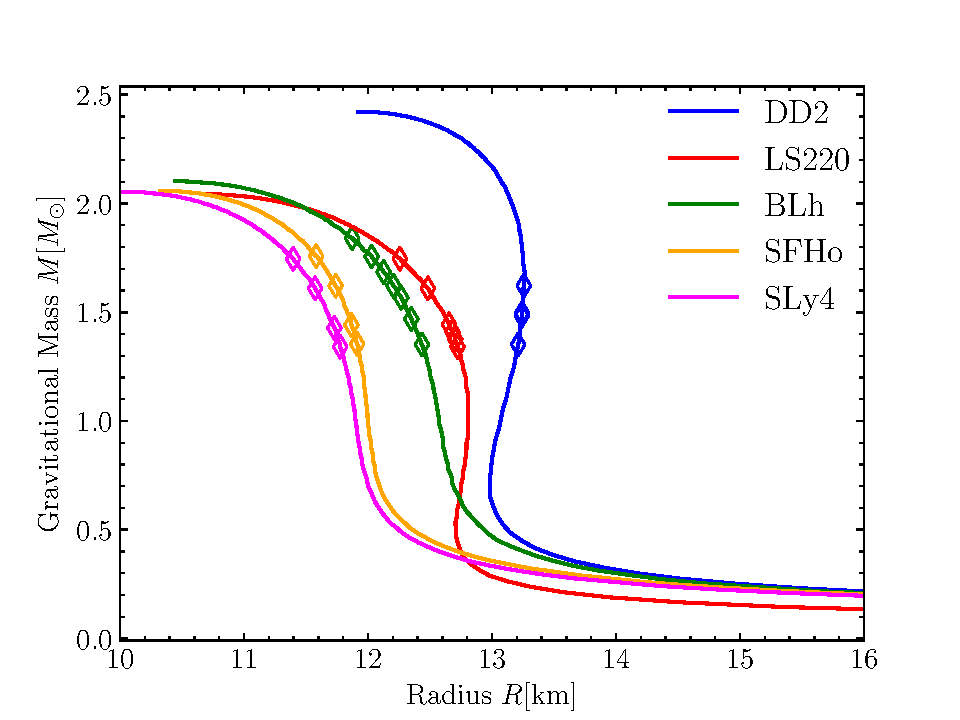
\includegraphics[width=0.49\textwidth]{tov_mr.pdf}
    \caption{Mass-radius relations for the EOSs used in this work. 
        Markers along the sequences indicate the NSs smulated in this work.}  
    \label{fig:method:tov_mr}
\end{figure}

For our models we employ $5$ finite-temperature, composition-dependent equations of state, namely the 
HS(DD2) (hereafter DD2) \cite{Typel:2009sy,Hempel:2009mc}, 
BLh, \cite{Bombaci:2018ksa}, 
LS220, \cite{Lattimer:1991nc}, 
HS(SFHo), (hereafter SFHo) \cite{Steiner:2012rk} and 
SLy4-SOR EOS (hereafter SLy4) \cite{daSilvaSchneider:2017jpg}.

All EOS include neutrinos $(n)$, protons $(p)$, nuclei, electrons, positrons, and photons
as important thermodynamic degrees of freedom.

The radii and maximum masses of neutron stars composed of the cold, neutrino-less $\beta$-equilibrium matter,
from these EOS, fall in line with the current astrophysical constraints, 
\textit{e.g.,} LIGO/Virgo constrain on tidal deformability 
\citep{TheLIGOScientific:2017qsa,Abbott:2018wiz,De:2018uhw,Abbott:2018exr}

All EOS models have symmetry energy at saturation density that are in argeement with experimental limits.
Notably, the LS220 has a especially steep dependency of its symmetry energy on density (\textit{e.g.,} \cite{Lattimer:2012xj,Danielewicz:2013upa}. Thus, this EOS might predict too low symmetry energy below the saturation density. 

%% LS220
The LS220 EOS is based on a non-relativistic (liquid droplet) Skyrme model.
The absolute value of the nuclear bulk incompressibility is set to $220$~MeV, hence, the name.
The EOS includes surface effects and it models $\alpha$-particles as an ideal, classical
non-relativistic gas. For heavy nuclei, the single nucleus approximation is sued. 
%Thus, the the compressible, liquid-drop model with surface effects and composed of ideal gas of 
%particles and heavy nuclei is used to represent the non-homogeneous nuclear matter.
%Heavy nuclei are considered with single nucleus approximation. 
The Gibbs construction is used to model the transition between homogeneous and non-homogeneous matter.
LS220 does not satisfy the constraints from Chiral effective field theory \cite{Hempel:2017ikt}

%% DD2
DD2 (and SFHo) employs the statistical equilibrium to treat the ensemble of several thousands nuclei.
The high-density nuclear matter is treated via RMF approach for unbound nucleons \cite{Hempel:2009mc}.
The excluded volume mechanism is utilized for the phase transition from nuclei to homogeneous
nuclear matter (when densities approch the nuclear saturation density).
DD2 employs the linear, but density dependent coupling for modeling the mean-field nuclear interactions \cite{Typel:2009sy}.
It was however noted that DD2 is not in very good agreement with the so-called flow-constraint \cite{Danielewicz:2002pu}.

%% SFHo [more rephrasing needed!]
Similar to DD2, SFHo combines a statistical ensemble of numerous nuclei, under the assumption of nuclear
statistical equilibrium (NSE) to treat the homogeneous matter, 
with the relativistic mean field approach for the unbound nucleons to treat high-density homogeneous nuclear matter.
It however employs a different parameterizations and values for modeling the mean-field nuclear interactions, 
which is motivated by neutron star radius measurements from low-mass X-ray
binaries (\cite{Steiner:2012rk} and references therein).

The DD2 and SFHo are based on nuclear statistical equilibrium, but 
different parameterizations of the covariant Lagrangian which models the mean-field nuclear interactions.
In these EOSs a finite volume correction coupled to a relativistic mean field theory for treating high-density nuclear matte. However, between these EOSs mean-field nuclear interactions have different parameterizations and values.

%% SLy4
The SLy4 EOS eomplyed in this work is the finite temperature extension \cite{daSilvaSchneider:2017jpg}
of the basic SLY4 Skryme parametrisation for cold nuclear NS matter \cite{Douchin:2001sv}.
The extension includes the non-local isospin asymmetric terms as well as more sophisticated 
treatment of nuclear surface properties and consistent treatment of heavy nuclei size. 
Which is a more advanced version of LS220 treatment (model).
When the phase transition, between the uniform and non-uniform phases, occurs, the phase with lowest 
free energy is chosen, (first order transition).

%% BLh
BLh is a new finite temperature EOS \cite{Logoteta:2020yxf}
This EOS is a finite temperature extension of the cold, $\beta$-equilibrium EOS, \cite{Bombaci:2018ksa},
which was applied to model the BNS merger in \cite{Endrizzi:2018uwl}.
The equation of state is derived in the framework of non-relativistic Brueckner-Hartree-Fock approach.
where microphysical approach based on a specific nuclear interaction is employed for the homogeneous nuclear phase.
The interactions between nucleos are described through a potential derived perturbatively 
in Chiral-Effective-Field theory \cite{Machleidt:2011zz}
The two body interactions are modeled up to second (from the leading term) order, that are used to calculate the local potential. This potential includes $\Delta$-resonances possible excitation. 
Further, the potential is augmented with the three-nucleon force, with the addition of $\Delta$-excitations.
The three-nucleon force was calibrated to reproduce the symmetric nuclear matter at saturatuin density \cite{Logoteta:2016nzc}.
The non-homogeneous phase of the EOS is treated by smoothly connecting the high density BLh EOS to the low-density oart of the SFHo EOS.


\subsubsection{Finite temperature treatment}


Thermal effects are included a different way in these EOS. 
In particular particle correlations beyond the mean field approximation are included only in the BLh EOS.
In other EOS thermal effects enter in the nucleon effective mass, that depend on temperature and density.
These effects, however, are important for the thermal evolution of the NS matter.

%% LS220 and SLy4
In the EOSs that are based on the Skyrme effecrive nuclear interatcions, \textit{e.g.,} LS220 and SLy4
the thermal effects are added in the following form. 
Consider a zero temperature internal energy functional, which depends explicitly on the nuclear density.
The part of this functional that is resposible for interactions is divided into the 
subpart that represents the two-body nucleon-nucleon interactions, (it is quadratic in nuclear density) and a 
subpart that mimics the effect of many body nuclear forces (proportional to the nuclear density in certain power).
Then, both the single particle potentials as well as kinetic energy effective mass dependence play a role
in the temperature dependence of the nuclear effective interaction.
The single particle potential are computed via the variation of the internal energy with respect to the 
neutron and proton densities.
Thus, the smaller the effective masss the larger are kinetic energies and hence, hgiher matter temperature. 
If the entropy remains unchainched.
Thus, the finite temperature behavior of these EOSs is largely set by the nucleon effective mass.
%Then, the smaller the effective mass, the higher the temperature (assuming that entropy is unchanged).
For LS220, the nucleon mass is its bare nucleon mass (for any densities) \gray{so... $m_{N}^*=m_{N}$??}.
For SFHo, $m_N ^* / m_N = 0.76$ at saturation density. 
For DD2 $m_N^*/m_N = 0.56$ 
For BLh $\red{None}$ 
For SLy4 $m_N^*/m_N=0.70$ at saturation density. 
where $m_{N}^*$ is the effective nucleon mass and $m_N$ is the bare nucleon mass.

%% SFHo (and DD2??)
For the SFHo and DD2 EOS, the relativistic Lagrangian considers the $\sigma-$, $\omega-$ and $\rho-$
meson exchanges for descibing nuclear interactions, and the mean-field approximation is used
to solve the resulted Euler-Largrange equations. 
The thermal effects for various species are introduced via Fermi-Dirac distributions at finite temperatures.
Then, self consitent solution of the mean filed eqution introduces the temperature dependence into other 
thermodynamic quantities (through fiurst mesons and nucleon fields)

%% BLh
The BLh EOS employs a different approach to incorporate temperature effects.
The method is based on evaluating the free energy in the Brueckner-Hartree-Fock, which in turn requires,
the effective in-medium nuclear interactions to be defined (starting from the bare nuclear potential).
\gray{This effective interaction is obtained by solving
    the Bethe-Goldstone integral equation which describe the nucleon 
    scattering in the nuclear medium and properly takes into
    account the Pauli principle}.
Then, the nucleon single particle potentials are evaluated (via integration of the on-shell effective interaction matrix)
, which represent the mean field that a nucleon with a certain momenum experience surrounded by other nucleons.
The nucleon single particle potentials, then, allow to evaulate the free energy, and subsequently, 
other thermodynamic quantities.
Notable difference with other EOS discussed here is that the many-body correlations extend beyond the mean field approximation, and are not present in other EOS. 
This EOS was first employed for the BNS merger simulations in \cite{Bernuzzi:2020txg}.

\subsubsection{TOV}

To characterize these EOS, that employs very different microphyscis and finite temperature properties and their relation to the electron fraction, we consider the TOV solutions, presented on the figure \ref{fig:method:tov_mr}.
The maximum mass of a non-rotating NS that these EOSs support are $2.06$, $2.06$, $2.42$ $None$ $None$ 
for SFHo, LS220, DD2, BLh and SLy4 respectively. The NS radii, $R_{1.4}$, then $11.9$, $12.7$, $13.2$ $\red{None}$ $\red{None}$, which in turn is related to the pressure at half saturation density \cite{Lattimer:2012nd}. Thus we adopt the following naming convention for EOS. Those that lead to a NS with smaller radii are called "softer" and those that lead to a NS with larger radii are referred to as "stiffer" EOS.
Among considered, the DD2 is the stiffest EOS, while SLy4 is the softest.

%% =====================================================================================
%%
%%               C O D E -- W H I S K Y - T H C
%%
%% =====================================================================================


\section{Code}


\subsection{Initial Data}

For Each EOS considered, we compute the irrotational BNS configurations in quasi-circular orbit.
We employ the pseudo-spectral code \texttt{Lorene} \citep{Gourgoulhon:2000nn}, that 
solves the general relativistic initial data problem.
The initial separation (of the qusi-circular orbit) is chosen $\sim40$~km and that corresponds to $~2-3$ orbits before merger.

The EOS table used for the initial data computation is the minimum temperature slice
$(T\sim 0.5 - 0.1)$~MeV of the finite temperature EOS table used for the evolution.
The assumption of the neutrino-less beta-equilibrium is made.
At constant temperature, at lowest densities, the photon energy (radiation) is a dominant contribution to 
pressure. Thus, we substruct this contribution from the tables.
%Addiitionally, the assuming constant temperature, we also remove the photon (radiation) energy contribution to the pressure (which dominates at the lowest densities)

The EOS table for the minimum temperature slice of the EOS table used for the evolution assuming neutrino-less beta-equilibrium.
Assuming constant temperature, we also remove the photon energy contribution to the pressure.

%In the evolution code, passing the initial data, the mapping is done from the zero temerature
In the evolution code, the electron fraction is set by the beta equilibrium condition. 
The specific internal energy is reset in accordance with minimum temperature slice of the EOS table used for evolution.

Errors present in the initial data in introduced during the mapping result in a small oscillations of netron stars.
In terms of relative changes in central density these amounts to $\sim2-3\%$ \cite{Radice:2018pdn}


\subsection{Evolution with \texttt{WhiskyTHC}}


In this part we review the numerical relativity code that was used to model binary neutron star mergers analyzed in this thesis.
The part is based on the David Radice PhD thesis where most of the methods are discussed \cite{Radice:2013apa}, and on the published results and regarding code structure and \cite{Radice:2012cu,Radice:2013xpa,Radice:2013hxh,Radice:2015nva}.

In order to perform numerical simulations of fluid flow, accurate numerical codes are essencial. Codes that flux-conservative finite-difference HRSC schemes offer a ciertain degree of simplicity, while high-order finite volume schemes are more computationally expensive (as they require solution of multiple Riemann problems at the interface between regions) \cite{Reisswig:2009us,Shu:2001rep} as well as complex averaging and de-averaging procedures \cite{Tchekhovskoy:2007zn}.

The \texttt{THC} code is the Templated-Hydrodynamics Code developed using the \texttt{Cactus} framework \cite{Goodale:2003}. In \texttt{THC}, the state-of-the-art flux-vector splitting scheme are employed. The "templated" in the code name stands for a modern paradigm in C++ programming, the templated programming, where a part of the code can be generated from the prescribed templates at compiling time (\textit{e.g.,} \cite{Yang:2001})

The \texttt{THC} has several primitive cariable reconstruction schemes implemented, such as MP5, classical monotonicity preserving \cite{Suresh:1997,Mignone:2010} the weighted essentially non oscillatory (WENO) schemes WENO5 and WENO7 \cite{Liu:1994,Jiang:1996,Shu:1997} and two bandwidth-optimized WENO schemes WENO3B and WENO4B \cite{Martin:2006,Taylor:2007}, contracted for modeling the compressible turbulence. Note, that the number in scheme name stands for a formal order of accuracy.

\texttt{WhiskyTHC} is a result of combination of two \texttt{Whisky} \cite{Baiotti:2004wn} and \texttt{THC} \cite{Radice:2012cu}. High-order flux-vector splitting finite-differencing techniques came from the former, while the module for the recovery of the primitive quantities as well as the equation of state framework from the latter \cite{Galeazzi:2013mia}. Tabulated temperature and composition dependent equation of states can be used.

Overall, \texttt{WhiskyTHC} solves the equations of general-relativistic hydrodynamics in conservation form \ref{eq:theory:grhdeq_thc} using a finite difference scheme. \red{tripple check the FD is used for space time evol and central FV method is for hydro}
The flux reconstruction is done in local-characteristic variables using the MP5 scheme, see \textit{e.g.,} \cite{Rezzolla:2013} \red{CHECK}.
The space-time is evolved using the CCZ4 formulation \ref{eq:theory:ccz4equations}, solved via finite difference code publicly available through \texttt{Einstein Toolkit}, \cite{McLachlan,Loffler:2011ay}.\red{CHECK}.
There, the central stencil is used throughout, and only terms associated with the advection along the shift vector are treated using the upwinded by one grid point stencil. The accuracy of the scheme is available at 6th and 8th order, while 4th is commonly employed. In addition, the fifth order Kreiss-Oliger style artificial dissipation \cite{Kreiss:1973} is added to aid with non-linear stability.

The code is build on the \texttt{Carpet} AMR driver \cite{Schnetter:2003rb} from the \texttt{Cactus} computational toolkit \cite{Goodale:2003}, incorporating a provided by \texttt{Carpet} Berger-Oliger-style mesh refinement \cite{Berger:1989,Berger:1984} with subcycling in time and refluxing. \textcolor{red}{in Thesis it is said, -- no refluxing was done yet}

To treat the vacuum region, the code utilizes common, 'atmosphere' approach. The atmosphere is referred to an artificial density floor in the simulation domain. It is introduced in order to tackle the challenges arising when considering boundary between the fluid and vacuum in Eulerian (relativistic) hydrodynamics codes \cite{Galeazzi:mThesis:2008,Kastaun:2006,Millmore:2009dk}. 
The defining property of the atmosphere is that the rest mass density and coordinate velocity are reset to a floor values once the former falls below a certain threshold value during the evolution \cite{Font:2001ew,Baiotti:2004wn}. While showing a reasonable results in second order codes, in higher order ones the numerical oscillations lead to the creation of vacuum nonetheless, that in light of the aforemention atmosphere effect result in the mass and energy violation \cite{Radice:2011qr}. For codes that rely on characteristic variables, the degeneracy in low-density, low-temperature limits also plagues the computation. This problem is the main reason behind the popularity of robust shock capturing codes, even though they are of first order in the general-relativistic hydrodynamics codes. Vacuum treatment for higher order codes is of main challenges to overcome.

There are several approaches in how to treat atmosphere. 

\textit{Standard atmosphere Treatment} or \textit{"ordinary MP5 approach"} is based on setting density that falls below $(1+\epsilon)\rho_{\text{atmo}}$ to the atmosphere density, velocity to zero and internal energy to the one prescubed by the polytropic EoS. The $\rho_{\text{atmo}}$ is usually related to a certain characteristic density, \textit{e.g.,} maximum density at the beginning of the simulation as $\rho_{\text{atmo}} = 10^{-7,-9}\rho_{\text{max}}$. The tolerance parameter $\epsilon$ is usually set to $10^{-2}$ and accounts for excessive oscillations of the fluid–vacuum interface. 

\textit{An Improved Atmosphere Treatment} or \textit{"MP5+LF"} In this approach the component-wise Lax-Friedrichs flux split is turned on when a certain density is reached. This increases the dissipation of the scheme and allows to avoid problems arising in characteristic reconstruction, associated with the degeneracy of the characteristic variables close to vacuum. Unfortunately, if the ejection of low velocity and density matter is concerned, this approach may yield oscillatory solutions and thus creates artifacts. 

\textit{Positivity Preserving Limiter} is an approach discussed in \cite{Radice:2013apa} based on the use of PPL proposed in \cite{Hu:2013}. \gray{Here we provide a brief overview}. \red{No, we not}.
\gray{While for a simplified case of classical gas dynamics it might require a lower timestep, in the general relativistic case and general tabulated EOS, the positivist of pressure is difficult to assure due to complexity of the energy source terms. It can be mitigated by enforcing a floor value on the pressure}. 
Note, that adopting a positivity preserving limiter to treat the transition between matter and vacuum, still implies replacing the vacuum with low density fluid at rest, is not a physically accurate approach. That would rely on treating the transition as a free boundary (see \textit{e.g.,} \cite{Kastaun:2006}) The advantage of positivity preserving limiter with respect to a classical atmosphere treatment, is that it allows to have a value of $\rho_{\text{atmo}}$ that does not require further tuning and can be arbitrary small, and assure that the solution is locally conserved. 
\textcolor{red}{In our models} we employ this approach as follows, at the beginning of the simulations we set the floor density, relying in the subsequent evolution on a positivity preserving limiters to ensure the atmosphere well behavior. Due to negligible density of the atmosphere its accretion has a negligible effect on the evolved object. 

For the extensive tests of different reconstruction methods and atmosphere treatment we refer to the \cite{Radice:2013apa}.


\subsection{Hydrodynamics}



\red{THE IDEA IS THAT YOU PUT MAIN EQ AND THEORY INTO THEORY AND HERE JUST USE THE 'PAPER' STUFF}

The code evolves the proton and neutron number densities, $n_n$ and $n_p$
respectively, as 

\begin{equation}
\label{eq:wthc:pndens}
\nabla_\nu (n_p u^\mu) = R_p^\mu \ \ , \ \ 
\nabla_\nu (n_n u^\mu) = R_n^\mu \ .
\end{equation}

\gray{in Radice2016dwd it is $\nabla_{\alpha}(n_e u^{\alpha}) = R$}

\gray{in Galezzi2013, for Whisky, the equations are separate for baryon and leptons: $\nabla_{\alpha}(n_bu^{\alpha})=0$ and $\nabla_{\alpha}(n_eu^{\alpha})=N$, where the $n_b$ and $n_e$ are the baryon and electron number densities respectively.}

Here $u^{\mu}$ is the fluid four-velocity, $R_p = -R_n$ is the net
lepton number deposition rate due to the absorption and emission of neutrinos 
and antineutrinos (\red{see Section XXX})

The $R_{p,n}$ is computed according to the neutrino M0 scheme \cite{Radice:2016dwd,Radice:2018pdn}

The number densities are related as $n_p=Y_e n$ where $n = n_p + n_e$ is the baryon 
number density and $Y_e$ is electron fraction.

The matter of a neutron star is approximated with ideal fluid with stress-energy tensor

\begin{equation}
T_{\mu\nu} = \rho h u_{\mu} u_{\nu} + Pg_{\mu\nu}
\end{equation}

where $\rho=m_{\text{b}} n$ is the baryon rest-mass density, 
$n$ the baryon number density, $m_{\text{b}} \simeq 10^{-24}\,$g 
the neutron mass, 
\gray{if Galezzi13 it is nucleon mass which is actrually related to the EOS.}
$h=1+\epsilon + P/\rho$ the specific enthalpy, 
$\epsilon$ the specific internal energy (energy density),
and $P$ is \gray{total isotropic} pressure.

Written in a covariant form, the Euler equation for balance of energy and momentum reads

\begin{equation}
\label{eq:wthc:euler}
\nabla_\nu T^{\mu\nu} = Q u^{\mu} \ ,
\end{equation}

\gray{in Radice2016dwd it is $\nabla_{\beta}T^{\alpha\beta}=\Psi^{\alpha}$
    with $\Psi^{\alpha} = Q u^{\alpha}$.
}
\gray{In the Galezzi:2013 it is $\nabla_{\alpha}T^{\alpha\beta}=\Psi^{\beta}$.
    There the $T^{\alpha\beta}$ accounts for the ordinary matter and for trappend neutrinos and photons, but it does not include free-streaming neutrinos. Assumed to be similar to the 'test-fluid' they are neglected in constracting RHS of the Eistein equations.
}

where $Q$ is the net energy deposition rate doe to absorption
and emission of neutrinos also treated with the M0 scheme.
\red{JUST PUT REFS TO THE EQs THAT ARE IN THE 'nuetrino' AND 'viscosity' sections}


\subsection{Numerical methods}


High resolution shock capturing methods are used to discritize equations 
\eqref{eq:wthc:euler} and \eqref{eq:wthc:pndens}.
Specifically, central Kurganov-Tadmor type scheme \cite{Kurganov:2000} with 
HLLE flux formula \cite{Einfeldt:1988}
and non-oscillatory reconstruction of the primitive variables with the MP5 scheme of
\cite{Suresh:1997}.

Shock capturing schemes require the presence of a low density atmosphere around neutron stars.
The constant value of $\rho_0 = m_p n \approx 6\times 10^4$~\gcm.

The rest-mass consirvation in the presence of artificial atmosphere is assured via 
positivity-preserving limiter from \cite{Radice:2013xpa}

The local number densities of neutrons and protons separately, are assured via 
multi-fluid advection method of \cite{Plewa:1998nma}

The outflow properties are extracted when the density exceeds the atmosphere density
by several orders of magnitude.

%% Spacetime evolution
The spacetime is evolved using the Z4c formulation of Einstein's equations
\cite{Bernuzzi:2009ex,Hilditch:2012fp} as implemented in the \texttt{CTGamma} code
\cite{Pollney:2009yz,Reisswig:2013sqa} which is part of the \texttt{Einstein Toolkit} 
\cite{Loffler:2011ay}.

The non-linear stability of evolution is assured via Kreiss-Oliger dissipation. 
The spacial discritisation is done via fourth-order finite-differencing implemented in \texttt{CTGamma}.

The method of lines, MOL, couples the space-time evolution and hydrodynamics. 

Time integrator of choice is strongly-stability preserving third-order Runge-Kutta scheme \cite{Gottlieb:2009}.
The timestep is regulated by the Courant-Friedrichs-Lewy (CFL) condition, that required CFL factor 
to be $<0.25$ for numerical stability. To assure taht the positivity-preserving limiter implemented in \texttt{WhiskyTHC} maintains the density positive, the CFL factor is set to $0.15$.


\subsection{AMR}


The code uses the Berger-Oliger conservative adaptive mesh renement (AMR) \cite{Berger:1984} with 
sub-cycling in time and \red{refluxing (Davids thesis does not have refluxing)} \cite{Berger:1989,Reisswig:2012nc} as provided by the \texttt{Carpet module} of the \texttt{Einstein Toolkit} 
\cite{Schnetter:2003rb}. 


\subsection{Neutrino scheme}


\begin{table}
    \caption{
        Weak reactions employed in our simulations and references for their implementation.
        In the left column, $\nu \in \{\nu_e, \bar{\nu}_e, \nu_{x}\}$ denotes any neutrino species, 
        $\nu_{x}$ any heavy-lepton neutrinos, $N \in\{n, p\}$ a nucleon, and $A$ any nucleus.
        In the central column the role of each reaction is highlighted, with "P" standing for 
        production, "A" for absorption opacity and "S" for scattering opacity. When two roles are
        indicated, the second refers to the inverse ($\leftarrow$) reaction.
        Table is taken from \cite{Radice:2018pdn}.
    }
    \label{tab:leakage}
    \begin{center}
        \begin{tabular}{lll}
            \hline\hline
            Reaction & Role &  Ref. \\ 
            \hline
            $p + e^- \leftrightarrow \nu_e + n $          & P,A & \cite{Bruenn:1985}  \\
            $n + e^+ \leftrightarrow \bar{\nu}_{e} + p $  & P,A & \cite{Bruenn:1985}  \\
            $e^+ + e^- \rightarrow \nu + \bar{\nu}$       & P & \cite{Ruffert:1995fs} \\
            $\gamma + \gamma \rightarrow \nu + \bar{\nu}$ & P & \cite{Ruffert:1995fs} \\
            $N + N \rightarrow \nu + \bar{\nu} + N  + N$  & P & \cite{Burrows:2004vq} \\
            $\nu + N \rightarrow \nu + N$                 & S & \cite{Ruffert:1995fs} \\
            $\nu + A \rightarrow \nu + A$                 & S & \cite{Shapiro:1983du} \\
            \hline\hline
        \end{tabular}
    \end{center}
\end{table}

\red{JUST Name the chemes and reference the equations}
\red{JUST PUT REFS TO THE EQs THAT ARE IN THE 'nuetrino' AND 'viscosity' sections}

\subsection{Code General Setup}



The simulation domain is a cube of $3.024$~km each side, whose center is at the center of mass pf the binary.
The AMR structure has $7$ refinemnt levels, with the finest convering both compact objects during the inspiral and the remnant postmerger.

We consider several resolution setups. Low resolution (LR) simulations have $h=246$~m, standard resolution (SR) 
have $h=185$~m and high resolution (HR) $h=123$~m for the final refinemnt level.

In the simulations where the neutirno M0 scheme is included, it is switched on shortly before the merger. 
The equations \eqref{eq:method:whisky:eq7} and \eqref{eq:method:whisky:eq9} are solved on the uniform spherical grid
with radius $\approx 756$~km, and resolution $n_r\times n_{\theta}\times n_{\phi} = 3096 \times 32 \times 64$
grid points.

A subset of models discussed in this thesis include the effective treatment of viscosity. 

We consider \red{$33$} distinct binary with total masses $\red{[None,None]}$ and mass-ratio $q\in[1.00,1.82]$.
In all models the neutrino leackage plus M0 scheme. Most models were computed at at least two resolutions. 
Most our models also include the effect of subgrid turbulence, viscosity.

\gray{Summary of all results in given in the table...}

\gray{Each run is nameed as}

\gray{We simulate each model for at least $\red{None}$~ms after the merger or a few milliseconds after BH formation}


%% =====================================================================================
%%
%%               P O S T - P R O C E S S I N G
%%
%% =====================================================================================


\section{Postprocessing tools and methods}


In order to investigate the neutron star merger dynamics and outflowing material we imploy the following methods and tools.

In order to study and compara on a quantiative level properties of outflow, disk and remnant we employ the mass-averaged quantities and for a quantity $f$ they are computed as 
\begin{equation}
\langle f \rangle = \frac{\sum_i f(m_i)m_i}{\sum_i m_i}
\end{equation}
where $m_i$ is the mass contained in the $i$-th bin.


\subsection{Disk \& Remnant}

It is common to discuss the post-merger state of the binary neutron star systems in terms of the remnant, a neutron star or a black hole, and a disk or torus. However there is not unified convention in how to define the latter and separate it from the former. 

In the case where the remnant is a BH, the disk common disk definition is the matter outside the apparent horizon, (\eg, \cite{Dietrich:2015iva,Dietrich:2016hky}). 
However, owing to the disk accretion onto a black hole, the extraction time is a crutual paramter, and unfortunately is not consistent in the literature, (\eg $\sim1$~ms in \cite{Dietrich:2015iva,Dietrich:2016hky} and $\sim30$~ms in \cite{Sekiguchi:2016bjd}).

In the case where the remnant is a neutron star, the disk definition usually includes the density cut. For instance, in \cite{Radice:2018pdn,Kiuchi:2019lls,Vincent:2019kor} the disk is assumed to encompass the matter with $\rho < 10^{13}$~\gcm. 
The threshold $\rho\sim 10^{13}$~\gcm corresponds to the point in the remnant where
the angular velocity profiles becomes approximately Keplerian, \citep[\eg][]{Shibata:2005ss,Shibata:2006nm,Hanauske:2016gia,Kastaun:2016elu}.
The extraction time here is also important, but less so, as we find that the accretion on the NS is considerably slower.

Overall, we estimate that these differences can amount to a systematic factor of a few,
which we employ for the statistical analysis in section \ref{sec:stat:anal}

% In this thesis we define the disk as a matter that satisfies two criteria $\alpha > 0.15$ and $\tho < 10^{13}\gcm$, where $\alpha$ is the lapse function (see section \ref{sec:theory:gr3p1}).

We compute the baryonic mass of the disks is computed as the volume integral of the conserved rest-mass density $D=\sqrt{\gamma}~W\rho$,

\begin{equation}
\label{eq:method:mdisk}
M_{\text{disk}} = \int D \dd^3 x
\end{equation}

from 3D snapshots of the simulations in postprocessing.



%% In \cite{Sekiguchi:2016bjd}, the disk mass is extracted at
%% ${\approx} 30$~ms outside the AH. In \cite{Radice:2018pdn}, the disk mass is computed
%% as the baryonic mass outside the AH at BH formation, while for NS
%% remnants the criterion $\rho < 10^{13}$ g cm$^{-3}$ is used. 
%% In \cite{Kiuchi:2019lls} for both BH and NS outcome the $\rho < 10^{13}$ g cm$^{-3}$ 
%% criterion is used and time of the extraction is not specified. 
%% In \cite{Vincent:2019kor} the density criterion is the same, however the simulations 
%% are significantly shorter (${~\sim 7.5}$~ms) than in other
%% works. Overall, we estimate that these differences can amount to a
%% systematic factor of a few.



\subsection{Density modes}

%% FROM THE LETTER 

The hydrodynamic instability is monitored by a decomposition in Fourier modes
$e^{-\i m\phi}$ of the Eulerian rest-mass density on the equatorial plane 
[see Eq.~(1) of \citep{Radice:2016gym}] and characterized by the
development of a $m=2$ followed by a $m=1$ mode 
\citep{East:2015vix,Paschalidis:2015mla,Radice:2016gym,Lehner:2016wjg,Bernuzzi:2013rza,Kastaun:2014fna}.
In the short-lived remnant (LS220) the $m=1$ mode
is subdominant with respect to the $m=2$, and it reaches a maximum close to the collapse
\citep{Bernuzzi:2013rza}. Instead, in the long-lived remnant (DD2) the $m=1$
becomes the dominant mode at $\sim$20~ms and persists throughout the
remnant's lifetime, while the $m=2$ efficiently dissipates via
gravitational-wave emission \citep{Bernuzzi:2015opx,Radice:2016gym}.

%% FROM THE PAPER 

During the post-merger evolution the neutron star oscillates. The most prominant modes are quasiradial mode $F$ ($m=0$), the $m=2$ $f$-model and non-linear combinations of them \citep[\eg][]{Shibata:2000jt,Stergioulas:2011gd}.

It has also been shown that the $m=1$, one-armed spiral instability, is present in the remnant of neutron star mergers \citep{Paschalidis:2015mla,Radice:2016gym,East:2016zvv}.

In order to investigate the dynamical instabilities in our simulations we 
project the rest-mass density onto spherical harmonics,
or, in other words, we perform the complex azimuthal mode decomposition of,
the conserved rest-mass density.
For simplicity we consider only $\rho(x,y,z=0,t)$, 
\ie restrict our analysis to the orbital plane $z=0$

\red{DOUBLE check the presence of Gamma and W}
%% \begin{equation}
%% \label{eq:modes}
%% C_m = \int \rho(x,y,z=0,t) W e^{-i m \phi} \sqrt{\gamma} %% \text{d}x \text{d} y \, ,
%% \end{equation}
\begin{equation}
\label{eq:modes}
C_m(t) = \int \rho(x,y,z=0,t) e^{-i m \phi(x,y)} \text{d}x \text{d} y \, ,
\end{equation}
(see \eg~\citet{Baiotti:2009gk}).

% where %% $\rho$ is the rest mass density, 
% $\gamma$ is the determinant of the three-metric and $W$ is the
% Lorentz factor between the fluid and the Eulerian observers. 

Note that the above quantities are gauge dependent.

\red{Dietrich in his thesis thinks that the growing m=1 mode is "We can not
    exclude the possibility that the growing m = 1 mode is triggered by numerical effects,
    but we think that it is a physical hydrodynamical effect due to mode couplings."
    Page 53 of the thesis
}

In addition, friequencies of the modes can be computed with the Fourier analysis of the $\rho_{\text{max}}$ and projections $C_{m}$. We resort it for the future work, as in this work we are interested inly in their magnitude. 





\subsection{Angular momentum}

\red{First, white that in GR the angular momentum is not clearly defined}

%% FROM LETTER 

From the fluid's stress energy tensor,
we compute the angular momentum density flux $J_r = T_{ra}(\partial_\phi)^a$,
where $\phi$ is the cylindrical angular coordinate;
angular momentum is conserved if $(\partial_\phi)^a$ is a Killing vector.

%% FROM PAPER 

The fluid's angular momentum analysis in the remnant and disk is performed
assuming axisymmetry (see Appendix~\ref{app:ang} for derivation).
That is, we assume $\phi^{\mu} = (\partial_{\phi})^{\mu}$ to be a Killing
vector. Accordingly, the conservation law
\begin{equation}
\partial_t(T^{\mu\nu}\phi_{\nu}n_{\nu}\sqrt{\gamma}) -
\partial_i(\alpha T^{i \nu}\phi_{\nu}\sqrt{\gamma}) = 0 \ ,
\end{equation}
where $n^\mu$ is the normal vector to the spacelike hypersurfaces of
the spacetime's $3+1$ decomposition, 
implies the conservation of the angular momentum
\begin{equation}
J = % \int j dV = 
%- \int \, T_{\mu\nu}n^{\mu}\phi^{\nu}\,\dd ^3x = 
-\int \,
T_{\mu\nu}n^{\mu}\phi^{\nu}\,\sqrt{\gamma}\, \dd^3 x\ .
\end{equation}
In the cylindrical coordinates $x^i=(r,\phi,z)$ adapted to the symmetry
the angular momentum density is  
\begin{equation}
j = %-
\rho h W^2 v_{\phi} \ ,
\label{eq:method:ang_mom}
\end{equation}
and the angular momentum flux is 
\begin{equation}
\alpha\sqrt{\gamma}T^r _{\nu}\phi^{\nu} =
\alpha\sqrt{\gamma}\rho h W^2 (v^{r}v_{\phi}) .
\end{equation}


\subsection{Ejecta}


To model and study the electromagnetic counterparts to mergers, the amount and properties of the material
leaving the system are needed.
The matter expelled at high velocity may ultimately become unbound from the central gravitational
potential. There are two indicators commonly adopted to mark the unbound matter.

\subsubsection{The Geodesic criterion}

Assuming that the spacetime is stationary, the $\partial_t$ is the killing vectory \red{confirm}, 
the four-velocity, $u_t$, (along the time-like killing vector), is a constant of motion for geodesics. 
Additionally, if the space is asymptotically flat, at infinity the $u_t = -W$, where $W$ is the fluid element Lorentz factor. Then, if a fluid element has $u_t < -1$, it may be considered unbound \red{as it will retain the non-zero positive velocity at infinity}. 
The fluid reaches an asymptotic velocity 
\begin{equation}
\upsilon_{\infty} \simeq \sqrt{2E_{\infty}} = \sqrt{(1-u_t ^2)}.
\end{equation}
The criterion can be through of as considering the fluid to be made of isolated particles that follow the geodesics. Indeed, the effects of equation of state, fluids pressure gradient, internal energy and heating (\eg, due to an $r$-process (\red{see section XXX})) are neglected. The space time is also assumed to be static.
Strictly speaking, none of these assumptions is fulfilled in the BNS post-merger environment. However, this criterion is widely used in the literature \citep[\eg][]{Radice:2018pdn,Vincent:2019kor}.
Note that the geodesic criterion above neglects the fluid's pressure and might underestimate the ejecta mass.

\subsubsection{The Bernoulli criterion}

From the relativistic Bernoulli equation \citep{Rezzolla:2013}, it follows
that for a stationary relativisitc flow, the $hu_t$ is constnat along the 
fluid worldliens. Here $h$ is the (relativistic) enthalpy, which is
defined up to a constant factor. 
If at the spatial infinity the enthalpy is set so $h\rightarrow-1$, 
\red{in Vincent it is $h\leftarrow 1$}
the condition $hu_t < -1$ would mark the unbound matter 
(as in the assymptotically flat space-time the $u_t = -W$ for the flow particles following geodesics).

The associated asymptotic velocity is calculated as 
\begin{equation}
\upsilon_{\infty} \simeq \sqrt{2 (h (E_{\infty}+1)-1)}. 
\end{equation}

The criterion can be regarded as assuming all the internal energy of the fluid 
gets added to the fluid kinetic energy, as the fluid decompresses \red{(pressure drops?)}.

The $r$-process nucleosynthesis that occurs in the outflow deposits the energy.
\red{In Vincent it is assumed that the difference in binding energy between the 
    particles in NSE at a given $\rho$, $T$ and $Y_e$, and their binding energy at
    the same $Y_e$ but low $\rho$ and $T$ is added/substracted from the fluid's kinetic energy.
    Out-of-NSE evolution and effects this neglected \citep[][see]{Foucart:2016vxd}
    [BUT I AM NOT SURE IF THIS IS THE CASE FOR OUR SIMULATIONS! MAYBE NOT!]}

This criterion has been found to estimate more accurately the amount of unbound material \citep{Foucart:2015gaa}
However, as was also found that the Bernoulli criterion leads to up to twice the amount of ejecta detected in comparion with the geodensic criterion, if the estimation is done within a given volume \citep{Kastaun:2014fna}.

We adopt the geodesic criterion to study the "burst-like", short outflows,
such as dynamical ejecta, where the pressure gradient is not expected to make a significant contribution.
For the steady-state outflows, like postmerger winds we adopt the Bernoulli criterion.

The term ejecta would refer to the material gravitationaly unbound according to eather of the criteria.




All considered mass ejecta are calculated on a coordinate sphere at $R \simeq 294$km. 
\red{untill afterglow}




%% =====================================================================================
%%
%%               R E S U L T S
%%
%% =====================================================================================


\section{Results}


\red{
    To be defined: \\
    Chirp pass \\
    Gravitational and Baryonic masses
}

In this chapter we review the findings of \citet{Nedora:2019jhl} and \citet{Nedora:2020pak}
and investigate the long-term \pmerg{} evolution of the binary neutron star. 

Such studies are of high astrophysical importance as the ejecta of matter that occur 
on various timescales \pmerg{} undergoes \rproc{} and produces observable EM emission. 
The discussion of the \rproc{} and EM transits themselves, we resort for the chapter \red{chap:coutnerparts}.


\subsection{Simulations}




%% --------------------------------
%% TAB SIM SUMMARY
%\begin{table*}
\begin{sidewaystable}
\begin{center}
\captionsetup{width=1.0\linewidth}
    \caption{
      Summary table of all the simulations and dynamical ejecta properties. The columns contain
      the following information, starting from the left. Equation of
      state, mass-ratio, available resolutions,
      inclusion of subgrid turbulence, time of the
      simulation end, time of the BH formation for LR, SR, HR
      resolutions separately, time of last output, time the disk mass
      is extracted, disk mass, mass of the
      dynamical ejecta, mass-averaged electron fracton, terminal
      velocity and RMS angle (from the binary plane) for dynamical ejecta. For all
      data except $t_{BH}$, $t_{\text{end}}$ and $t_{\text{disk}}$, the value that is given is a mean value across resolutions, with an error estimated as one
      standard diviaion from the mean. In case where only one
      resolution is present, the error is assumed to be $20\%$ of the
      value. Adopted from \citet{Nedora:2020pak}.
    }
      %% \newtxt{For discussions on errors and convergence see \citep{Radice:2018pdn,Bernuzzi:2020txg}.
      %% The model data are available online at \citep{vsevolod_nedora_2020_4159619}.
%%       }
\scalebox{0.70}{
\begin{tabular}{c c c c c c c c c c c c c}
    \hline\hline
    EOS & $q$ & $\tilde{\Lambda}$ & Resolution & GRLES & $t_{\text{end}}$ & $t_{\text{BH}}$ & $t_{\text{disk}}$ & $M_{\text{disk}} ^{\text{last}}$ & $\md$ & $\langle \yd \rangle$ & $\langle \vd  \rangle$ & $\langle \theta_{\text{ej}} ^{\text{d}} \rangle$ \\
    &   &   &  &  & [ms] & [ms] & [ms] &   & $[10^{-2} M_{\odot}]$ &   & $[c]$ &   \\ 
    \hline
    \hline
    BLh & 1.00 & 541 & \texttt{LR SR HR} & \cmark & $43.3$ $91.8$ $23.1$ & $>43.3$ $>91.8$ $>23.1$ & 23.1 & $0.166^{+0.052} _{-0.052} $ & $0.14^{+0.02} _{-0.02} $ & $0.27^{+0.01} _{-0.01} $ & $0.17^{+0.01} _{-0.01} $ & $39.65^{+0.35} _{-0.35} $ \\
    BLh & 1.00 & 541 & \texttt{LR SR} & \xmark & $15.9$ $103.2$ $ $ & $>15.9$ $>103.2$ $ $ & 15.6 & $0.261^{+0.008} _{-0.008} $ & $0.12^{+0.01} _{-0.01} $ & $0.27^{+0.01} _{-0.01} $ & $0.16^{+0.01} _{-0.01} $ & $38.80^{+0.44} _{-0.44} $ \\
%%  BLh & 1.00 & 541 & \texttt{LR SR} & \xmark & $36.9$ $15.5$ $ $ & $>36.9$ $>15.5$ $ $ & 36.6 & $0.182^{+0.091} _{-0.091} $ & $0.21^{+0.04} _{-0.04} $ & $0.26^{+0.01} _{-0.01} $ & $0.18^{+0.01} _{-0.01} $ & $36.29^{+0.24} _{-0.24} $ \\
    \hline
    BLh & 1.18 & 539 & \texttt{LR} & \cmark & $69.4$ $ $ $ $ & $>69.4$ $ $ $ $ & 69.0 & $0.202^{+0.101} _{-0.101} $ & $0.30^{+0.06} _{-0.06} $ & $0.18^{+0.04} _{-0.04} $ & $0.19^{+0.04} _{-0.04} $ & $33.65^{+6.73} _{-6.73} $ \\
    BLh & 1.18 & 539 & \texttt{LR} & \xmark & $16.4$ $ $ $ $ & $>16.4$ $ $ $ $ & 15.9 & $0.229^{+0.115} _{-0.115} $ & $0.25^{+0.05} _{-0.05} $ & $0.16^{+0.03} _{-0.03} $ & $0.20^{+0.04} _{-0.04} $ & $30.86^{+6.17} _{-6.17} $ \\
    \hline
    BLh & 1.34 & 539 & \texttt{LR SR} & \cmark & $63.4$ $9.8$ $ $ & $>63.4$ $>9.8$ $ $ & 9.8 & $0.192^{+0.004} _{-0.004} $ & $0.25^{+0.05} _{-0.05} $ & $0.14^{+0.04} _{-0.04} $ & $0.17^{+0.00} _{-0.00} $ & $28.79^{+5.00} _{-5.00} $ \\
    BLh & 1.34 & 539 & \texttt{LR} & \xmark & $18.0$ $ $ $ $ & $>18.0$ $ $ $ $ & 18.0 & $0.211^{+0.106} _{-0.106} $ & $0.19^{+0.04} _{-0.04} $ & $0.17^{+0.03} _{-0.03} $ & $0.17^{+0.03} _{-0.03} $ & $33.39^{+6.68} _{-6.68} $ \\
    \hline
    BLh & 1.43 & 540 & \texttt{LR SR} & \cmark & $35.1$ $59.6$ $ $ & $>35.1$ $>59.6$ $ $ & 33.8 & $0.265^{+0.001} _{-0.001} $ & $0.27^{+0.08} _{-0.08} $ & $0.19^{+0.03} _{-0.03} $ & $0.16^{+0.00} _{-0.00} $ & $34.49^{+3.59} _{-3.59} $ \\
    \hline
    BLh & 1.54 & 543 & \texttt{LR} & \cmark & $45.8$ $ $ $ $ & $>45.8$ $ $ $ $ & 53.8 & $0.324^{+0.162} _{-0.162} $ & $0.20^{+0.04} _{-0.04} $ & $0.17^{+0.03} _{-0.03} $ & $0.13^{+0.03} _{-0.03} $ & $31.21^{+6.24} _{-6.24} $ \\
    BLh & 1.54 & 543 & \texttt{LR} & \xmark & $17.4$ $ $ $ $ & $>17.4$ $ $ $ $ & 30.1 & $0.287^{+0.144} _{-0.144} $ & $0.22^{+0.04} _{-0.04} $ & $0.21^{+0.04} _{-0.04} $ & $0.16^{+0.03} _{-0.03} $ & $35.05^{+7.01} _{-7.01} $ \\
    \hline
    BLh & 1.66 & 538 & \texttt{LR SR} & \cmark & $64.6$ $20.1$ $ $ & $>64.6$ $1.8$ $ $ & 19.2 & $0.289^{+0.005} _{-0.005} $ & $0.42^{+0.05} _{-0.05} $ & $0.11^{+0.01} _{-0.01} $ & $0.12^{+0.01} _{-0.01} $ & $24.08^{+0.29} _{-0.29} $ \\
    \hline
    BLh & 1.82 & 532 & \texttt{LR SR HR} & \cmark & $12.0$ $17.5$ $9.6$ & $1.4$ $1.4$ $1.5$ & 5.9 & $0.170^{+0.001} _{-0.001} $ & $0.81^{+0.04} _{-0.04} $ & $0.03^{+0.01} _{-0.01} $ & $0.11^{+0.00} _{-0.00} $ & $6.53^{+0.65} _{-0.65} $ \\
    BLh & 1.82 & 532 & \texttt{LR SR HR} & \xmark & $53.8$ $26.3$ $45.2$ & $1.7$ $1.3$ $1.0$ & 43.2 & $0.098^{+0.049} _{-0.049} $ & $1.07^{+0.07} _{-0.07} $ & $0.03^{+0.01} _{-0.01} $ & $0.12^{+0.00} _{-0.00} $ & $6.27^{+0.53} _{-0.53} $ \\
    \hline
    \hline
    DD2 & 1.00 & 853 & \texttt{LR SR}    & \xmark & $92.0$ $110.2$       & $>92.0$ $>110.2$        & 9.4 & $0.154^{+0.052} _{-0.052} $ & $0.11^{+0.01} _{-0.01} $ & $0.25^{+0.00} _{-0.00} $ & $0.18^{+0.01} _{-0.01} $ & $38.07^{+0.52} _{-0.52} $ \\
    DD2 & 1.00 & 853 & \texttt{LR SR HR} & \cmark & $123.0$ $113.0$ $74.4$ & $>123.0$ $>113.0$ $>74.4$ & 8.2 & $0.111^{+0.040} _{-0.040} $ & $0.12^{+0.03} _{-0.03} $ & $0.27^{+0.01} _{-0.01} $ & $0.16^{+0.00} _{-0.00} $ & $40.03^{+0.71} _{-0.71} $ \\
    \hline
    DD2 & 1.20 & 847 & \texttt{LR SR HR} & \xmark & $37.3$ $91.0$ $55.2$ & $>37.3$ $>91.0$ $>55.2$ & 36.6 & $0.261^{+0.028} _{-0.028} $ & $0.21^{+0.08} _{-0.08} $ & $0.18^{+0.03} _{-0.03} $ & $0.17^{+0.01} _{-0.01} $ & $29.07^{+3.75} _{-3.75} $ \\
    DD2 & 1.22 & 847 & \texttt{LR SR HR} & \cmark & $42.7$ $107.3$ $19.8$ & $>42.7$ $>107.3$ $>19.8$ & 8.7 & $0.209^{+0.033} _{-0.033} $ & $0.25^{+0.02} _{-0.02} $ & $0.19^{+0.01} _{-0.01} $ & $0.17^{+0.01} _{-0.01} $ & $30.74^{+0.89} _{-0.89} $ \\
    \hline
    DD2 & 1.43 & 820 & \texttt{LR SR} & \cmark & $37.7$ $62.0$ $ $ & $>37.7$ $>62.0$ $ $ & 36.7 & $0.304^{+0.051} _{-0.051} $ & $0.70^{+0.64} _{-0.64} $ & $0.14^{+0.05} _{-0.05} $ & $0.14^{+0.01} _{-0.01} $ & $25.51^{+9.58} _{-9.58} $ \\
    \hline
    \hline
    LS220 & 1.00 & 715 & \texttt{LR SR} & \cmark & $27.0$ $27.1$ $ $ & $13.7$ $13.7$ $ $ & 16.1 & $0.073^{+0.032} _{-0.032} $ & $0.16^{+0.02} _{-0.02} $ & $0.25^{+0.02} _{-0.02} $ & $0.16^{+0.01} _{-0.01} $ & $35.70^{+0.78} _{-0.78} $ \\
    LS220 & 1.00 & 715 & \texttt{LR SR HR} & \xmark & $35.9$ $37.2$ $27.1$ & $33.4$ $16.1$ $15.4$ & 34.6 & $0.072^{+0.006} _{-0.006} $ & $0.16^{+0.06} _{-0.06} $ & $0.22^{+0.00} _{-0.00} $ & $0.16^{+0.01} _{-0.01} $ & $34.99^{+1.68} _{-1.68} $ \\
    \hline
    LS220 & 1.05 & 715 & \texttt{SR HR} & \xmark & $ $ $23.3$ $24.1$ & $ $ $17.3$ $13.9$ & 22.3 & $0.107^{+0.054} _{-0.054} $ & $0.16^{+0.02} _{-0.02} $ & $0.21^{+0.01} _{-0.01} $ & $0.16^{+0.01} _{-0.01} $ & $33.28^{+2.37} _{-2.37} $ \\
    LS220 & 1.11 & 717 & \texttt{SR HR} & \xmark & $ $ $25.1$ $24.4$ & $ $ $17.0$ $>24.4$ & 24.2 & $0.140^{+0.071} _{-0.071} $ & $0.22^{+0.03} _{-0.03} $ & $0.19^{+0.02} _{-0.02} $ & $0.18^{+0.02} _{-0.02} $ & $30.25^{+4.43} _{-4.43} $ \\
    \hline
    LS220 & 1.16 & 714 & \texttt{SR HR} & \cmark & $ $ $95.8$ $11.3$ & $ $ $68.9$ $>11.3$ & 95.5 & $0.306^{+0.153} _{-0.153} $ & $0.34^{+0.00} _{-0.00} $ & $0.22^{+0.00} _{-0.00} $ & $0.16^{+0.00} _{-0.00} $ & $34.08^{+1.00} _{-1.00} $ \\
    LS220 & 1.16 & 714 & \texttt{LR SR HR} & \xmark & $29.5$ $36.1$ $28.8$ & $>29.5$ $>36.1$ $24.1$ & - & - & $0.33^{+0.05} _{-0.05} $ & $0.17^{+0.01} _{-0.01} $ & $0.17^{+0.01} _{-0.01} $ & $30.01^{+0.64} _{-0.64} $ \\
    \hline
    LS220 & 1.43 & 710 & \texttt{LR SR} & \cmark & $19.8$ $28.5$ $ $ & $15.7$ $12.3$ $ $ & 19.6 & $0.178^{+0.072} _{-0.072} $ & $0.73^{+0.03} _{-0.03} $ & $0.16^{+0.02} _{-0.02} $ & $0.17^{+0.01} _{-0.01} $ & $26.77^{+3.50} _{-3.50} $ \\
    \hline
    LS220 & 1.66 & 707 & \texttt{LR SR} & \cmark & $6.8$ $8.0$ $ $ & $1.4$ $2.1$ $ $ & 2.0 & $0.068^{+0.008} _{-0.008} $ & $1.11^{+0.38} _{-0.38} $ & $0.07^{+0.01} _{-0.01} $ & $0.14^{+0.01} _{-0.01} $ & $13.18^{+1.33} _{-1.33} $ \\
    \hline
    \hline
    SFHo & 1.00 & 413 & \texttt{SR HR} & \cmark & $ $ $25.3$ $11.6$ & $ $ $6.0$ $4.0$ & 50.0 & $0.023^{+0.012} _{-0.012} $ & $0.40^{+0.07} _{-0.07} $ & $0.21^{+0.00} _{-0.00} $ & $0.19^{+0.01} _{-0.01} $ & $32.48^{+1.79} _{-1.79} $ \\
    SFHo & 1.00 & 413 & \texttt{LR SR HR} & \xmark & $3.2$ $7.7$ $9.0$ & $>3.2$ $4.1$ $3.8$ & 7.2 & $0.019^{+0.007} _{-0.007} $ & $0.28^{+0.07} _{-0.07} $ & $0.23^{+0.01} _{-0.01} $ & $0.21^{+0.01} _{-0.01} $ & $31.66^{+1.80} _{-1.80} $ \\
    \hline
    SFHo & 1.13 & 412 & \texttt{SR HR} & \cmark & $ $ $14.2$ $14.3$ & $ $ $6.3$ $>14.3$ & - & - & $0.44^{+0.12} _{-0.12} $ & $0.18^{+0.01} _{-0.01} $ & $0.23^{+0.01} _{-0.01} $ & $33.20^{+0.78} _{-0.78} $ \\
    SFHo & 1.13 & 412 & \texttt{LR SR HR} & \xmark & $16.5$ $19.3$ $15.2$ & $5.5$ $11.6$ $3.9$ & 15.1 & $0.046^{+0.041} _{-0.041} $ & $0.42^{+0.03} _{-0.03} $ & $0.17^{+0.03} _{-0.03} $ & $0.22^{+0.01} _{-0.01} $ & $29.63^{+4.39} _{-4.39} $ \\
    \hline
    SFHo & 1.43 & 414 & \texttt{LR} & \cmark & $19.6$ $ $ $ $ & $4.8$ $ $ $ $ & 18.9 & $0.201^{+0.101} _{-0.101} $ & $0.38^{+0.08} _{-0.08} $ & $0.14^{+0.03} _{-0.03} $ & $0.20^{+0.04} _{-0.04} $ & $29.20^{+5.84} _{-5.84} $ \\
    SFHo & 1.43 & 414 & \texttt{SR} & \cmark & $ $ $46.5$ $ $ & $ $ $>46.5$ $ $ & 50.8 & $0.241^{+0.121} _{-0.121} $ & $0.24^{+0.05} _{-0.05} $ & $0.19^{+0.04} _{-0.04} $ & $0.14^{+0.03} _{-0.03} $ & $32.86^{+6.57} _{-6.57} $ \\
    \hline
    SFHo & 1.66 & 408 & \texttt{LR SR} & \cmark & $11.2$ $16.8$ $ $ & $1.3$ $1.3$ $ $ & 11.6 & $0.177^{+0.153} _{-0.153} $ & $0.15^{+0.00} _{-0.00} $ & $0.07^{+0.00} _{-0.00} $ & $0.12^{+0.01} _{-0.01} $ & $10.39^{+1.14} _{-1.14} $ \\
    \hline
    \hline
    SLy4 & 1.00 & 402 & \texttt{LR SR} & \cmark & $10.5$ $13.1$ $ $ & $2.8$ $2.8$ $ $ & - & - & $0.09^{+0.02} _{-0.02} $ & $0.23^{+0.02} _{-0.02} $ & $0.27^{+0.02} _{-0.02} $ & $30.81^{+2.81} _{-2.81} $ \\
    SLy4 & 1.00 & 402 & \texttt{LR SR} & \xmark & $12.7$ $22.0$ $ $ & $2.7$ $13.8$ $ $ & 12.5 & $0.071^{+0.175} _{-0.175} $ & $0.31^{+0.20} _{-0.20} $ & $0.23^{+0.03} _{-0.03} $ & $0.22^{+0.01} _{-0.01} $ & $32.23^{+4.84} _{-4.84} $ \\
    \hline
    SLy4 & 1.13 & 402 & \texttt{LR SR} & \xmark & $8.4$ $20.3$ $ $ & $>8.4$ $13.0$ $ $ & 8.0 & $0.164^{+0.023} _{-0.023} $ & $0.59^{+0.07} _{-0.07} $ & $0.16^{+0.00} _{-0.00} $ & $0.24^{+0.01} _{-0.01} $ & $29.67^{+1.97} _{-1.97} $ \\
    \hline
    SLy4 & 1.43 & 399 & \texttt{SR} & \cmark & $ $ $40.3$ $ $ & $ $ $>40.3$ $ $ & 45.2 & $0.200^{+0.100} _{-0.100} $ & $0.20^{+0.04} _{-0.04} $ & $0.21^{+0.04} _{-0.04} $ & $0.15^{+0.03} _{-0.03} $ & $34.03^{+6.81} _{-6.81} $ \\
    \hline
    SLy4 & 1.66 & 397 & \texttt{SR} & \cmark & $ $ $7.2$ $ $ & $ $ $1.2$ $ $ & 3.9 & $0.138^{+0.069} _{-0.069} $ & $0.28^{+0.06} _{-0.06} $ & $0.05^{+0.01} _{-0.01} $ & $0.12^{+0.02} _{-0.02} $ & $8.43^{+1.69} _{-1.69} $ \\
    \hline\hline
\end{tabular}
\label{tab:sim}
}%scalebox
\end{center}
%\end{table*}
\end{sidewaystable}



%\usepackage{lipsum}% dummy text
%\begin{document}
    %\lipsum % Text before
%    \afterpage{%
%        \clearpage% Flush earlier floats (otherwise order might not be correct)
%        \thispagestyle{empty}% empty page style (?)
%        \begin{landscape}% Landscape page
%            \centering % Center table
%            \begin{tabular}{c c c c c c c c c c c c c}
%                \hline\hline
%                EOS & $q$ & $\tilde{\Lambda}$ & Resolution & GRLES & $t_{\text{end}}$ & $t_{\text{BH}}$ & $t_{\text{disk}}$ & $M_{\text{disk}} ^{\text{last}}$ & $\md$ & $\langle \yd \rangle$ & $\langle \vd  \rangle$ & $\langle \theta_{\text{ej}} ^{\text{d}} \rangle$ \\
%                &   &   &  &  & [ms] & [ms] & [ms] &   & $[10^{-2} M_{\odot}]$ &   & $[c]$ &   \\ 
%                \hline
%                \hline
%                BLh & 1.00 & 541 & \texttt{LR SR HR} & \cmark & $43.3$ $91.8$ $23.1$ & $>43.3$ $>91.8$ $>23.1$ & 23.1 & $0.166^{+0.052} _{-0.052} $ & $0.14^{+0.02} _{-0.02} $ & $0.27^{+0.01} _{-0.01} $ & $0.17^{+0.01} _{-0.01} $ & $39.65^{+0.35} _{-0.35} $ \\
%                BLh & 1.00 & 541 & \texttt{LR SR} & \xmark & $15.9$ $103.2$ $ $ & $>15.9$ $>103.2$ $ $ & 15.6 & $0.261^{+0.008} _{-0.008} $ & $0.12^{+0.01} _{-0.01} $ & $0.27^{+0.01} _{-0.01} $ & $0.16^{+0.01} _{-0.01} $ & $38.80^{+0.44} _{-0.44} $ \\
%                %%  BLh & 1.00 & 541 & \texttt{LR SR} & \xmark & $36.9$ $15.5$ $ $ & $>36.9$ $>15.5$ $ $ & 36.6 & $0.182^{+0.091} _{-0.091} $ & $0.21^{+0.04} _{-0.04} $ & $0.26^{+0.01} _{-0.01} $ & $0.18^{+0.01} _{-0.01} $ & $36.29^{+0.24} _{-0.24} $ \\
%                \hline
%                BLh & 1.18 & 539 & \texttt{LR} & \cmark & $69.4$ $ $ $ $ & $>69.4$ $ $ $ $ & 69.0 & $0.202^{+0.101} _{-0.101} $ & $0.30^{+0.06} _{-0.06} $ & $0.18^{+0.04} _{-0.04} $ & $0.19^{+0.04} _{-0.04} $ & $33.65^{+6.73} _{-6.73} $ \\
%                BLh & 1.18 & 539 & \texttt{LR} & \xmark & $16.4$ $ $ $ $ & $>16.4$ $ $ $ $ & 15.9 & $0.229^{+0.115} _{-0.115} $ & $0.25^{+0.05} _{-0.05} $ & $0.16^{+0.03} _{-0.03} $ & $0.20^{+0.04} _{-0.04} $ & $30.86^{+6.17} _{-6.17} $ \\
%                \hline
%                BLh & 1.34 & 539 & \texttt{LR SR} & \cmark & $63.4$ $9.8$ $ $ & $>63.4$ $>9.8$ $ $ & 9.8 & $0.192^{+0.004} _{-0.004} $ & $0.25^{+0.05} _{-0.05} $ & $0.14^{+0.04} _{-0.04} $ & $0.17^{+0.00} _{-0.00} $ & $28.79^{+5.00} _{-5.00} $ \\
%                BLh & 1.34 & 539 & \texttt{LR} & \xmark & $18.0$ $ $ $ $ & $>18.0$ $ $ $ $ & 18.0 & $0.211^{+0.106} _{-0.106} $ & $0.19^{+0.04} _{-0.04} $ & $0.17^{+0.03} _{-0.03} $ & $0.17^{+0.03} _{-0.03} $ & $33.39^{+6.68} _{-6.68} $ \\
%                \hline
%                BLh & 1.43 & 540 & \texttt{LR SR} & \cmark & $35.1$ $59.6$ $ $ & $>35.1$ $>59.6$ $ $ & 33.8 & $0.265^{+0.001} _{-0.001} $ & $0.27^{+0.08} _{-0.08} $ & $0.19^{+0.03} _{-0.03} $ & $0.16^{+0.00} _{-0.00} $ & $34.49^{+3.59} _{-3.59} $ \\
%                \hline
%                BLh & 1.54 & 543 & \texttt{LR} & \cmark & $45.8$ $ $ $ $ & $>45.8$ $ $ $ $ & 53.8 & $0.324^{+0.162} _{-0.162} $ & $0.20^{+0.04} _{-0.04} $ & $0.17^{+0.03} _{-0.03} $ & $0.13^{+0.03} _{-0.03} $ & $31.21^{+6.24} _{-6.24} $ \\
%                BLh & 1.54 & 543 & \texttt{LR} & \xmark & $17.4$ $ $ $ $ & $>17.4$ $ $ $ $ & 30.1 & $0.287^{+0.144} _{-0.144} $ & $0.22^{+0.04} _{-0.04} $ & $0.21^{+0.04} _{-0.04} $ & $0.16^{+0.03} _{-0.03} $ & $35.05^{+7.01} _{-7.01} $ \\
%                \hline
%                BLh & 1.66 & 538 & \texttt{LR SR} & \cmark & $64.6$ $20.1$ $ $ & $>64.6$ $1.8$ $ $ & 19.2 & $0.289^{+0.005} _{-0.005} $ & $0.42^{+0.05} _{-0.05} $ & $0.11^{+0.01} _{-0.01} $ & $0.12^{+0.01} _{-0.01} $ & $24.08^{+0.29} _{-0.29} $ \\
%                \hline
%                BLh & 1.82 & 532 & \texttt{LR SR HR} & \cmark & $12.0$ $17.5$ $9.6$ & $1.4$ $1.4$ $1.5$ & 5.9 & $0.170^{+0.001} _{-0.001} $ & $0.81^{+0.04} _{-0.04} $ & $0.03^{+0.01} _{-0.01} $ & $0.11^{+0.00} _{-0.00} $ & $6.53^{+0.65} _{-0.65} $ \\
%                BLh & 1.82 & 532 & \texttt{LR SR HR} & \xmark & $53.8$ $26.3$ $45.2$ & $1.7$ $1.3$ $1.0$ & 43.2 & $0.098^{+0.049} _{-0.049} $ & $1.07^{+0.07} _{-0.07} $ & $0.03^{+0.01} _{-0.01} $ & $0.12^{+0.00} _{-0.00} $ & $6.27^{+0.53} _{-0.53} $ \\
%                \hline
%                \hline
%                DD2 & 1.00 & 853 & \texttt{LR SR}    & \xmark & $92.0$ $110.2$       & $>92.0$ $>110.2$        & 9.4 & $0.154^{+0.052} _{-0.052} $ & $0.11^{+0.01} _{-0.01} $ & $0.25^{+0.00} _{-0.00} $ & $0.18^{+0.01} _{-0.01} $ & $38.07^{+0.52} _{-0.52} $ \\
%                DD2 & 1.00 & 853 & \texttt{LR SR HR} & \cmark & $123.0$ $113.0$ $74.4$ & $>123.0$ $>113.0$ $>74.4$ & 8.2 & $0.111^{+0.040} _{-0.040} $ & $0.12^{+0.03} _{-0.03} $ & $0.27^{+0.01} _{-0.01} $ & $0.16^{+0.00} _{-0.00} $ & $40.03^{+0.71} _{-0.71} $ \\
%                \hline
%                DD2 & 1.20 & 847 & \texttt{LR SR HR} & \xmark & $37.3$ $91.0$ $55.2$ & $>37.3$ $>91.0$ $>55.2$ & 36.6 & $0.261^{+0.028} _{-0.028} $ & $0.21^{+0.08} _{-0.08} $ & $0.18^{+0.03} _{-0.03} $ & $0.17^{+0.01} _{-0.01} $ & $29.07^{+3.75} _{-3.75} $ \\
%                DD2 & 1.22 & 847 & \texttt{LR SR HR} & \cmark & $42.7$ $107.3$ $19.8$ & $>42.7$ $>107.3$ $>19.8$ & 8.7 & $0.209^{+0.033} _{-0.033} $ & $0.25^{+0.02} _{-0.02} $ & $0.19^{+0.01} _{-0.01} $ & $0.17^{+0.01} _{-0.01} $ & $30.74^{+0.89} _{-0.89} $ \\
%                \hline
%                DD2 & 1.43 & 820 & \texttt{LR SR} & \cmark & $37.7$ $62.0$ $ $ & $>37.7$ $>62.0$ $ $ & 36.7 & $0.304^{+0.051} _{-0.051} $ & $0.70^{+0.64} _{-0.64} $ & $0.14^{+0.05} _{-0.05} $ & $0.14^{+0.01} _{-0.01} $ & $25.51^{+9.58} _{-9.58} $ \\
%                \hline
%                \hline
%                LS220 & 1.00 & 715 & \texttt{LR SR} & \cmark & $27.0$ $27.1$ $ $ & $13.7$ $13.7$ $ $ & 16.1 & $0.073^{+0.032} _{-0.032} $ & $0.16^{+0.02} _{-0.02} $ & $0.25^{+0.02} _{-0.02} $ & $0.16^{+0.01} _{-0.01} $ & $35.70^{+0.78} _{-0.78} $ \\
%                LS220 & 1.00 & 715 & \texttt{LR SR HR} & \xmark & $35.9$ $37.2$ $27.1$ & $33.4$ $16.1$ $15.4$ & 34.6 & $0.072^{+0.006} _{-0.006} $ & $0.16^{+0.06} _{-0.06} $ & $0.22^{+0.00} _{-0.00} $ & $0.16^{+0.01} _{-0.01} $ & $34.99^{+1.68} _{-1.68} $ \\
%                \hline
%                LS220 & 1.05 & 715 & \texttt{SR HR} & \xmark & $ $ $23.3$ $24.1$ & $ $ $17.3$ $13.9$ & 22.3 & $0.107^{+0.054} _{-0.054} $ & $0.16^{+0.02} _{-0.02} $ & $0.21^{+0.01} _{-0.01} $ & $0.16^{+0.01} _{-0.01} $ & $33.28^{+2.37} _{-2.37} $ \\
%                LS220 & 1.11 & 717 & \texttt{SR HR} & \xmark & $ $ $25.1$ $24.4$ & $ $ $17.0$ $>24.4$ & 24.2 & $0.140^{+0.071} _{-0.071} $ & $0.22^{+0.03} _{-0.03} $ & $0.19^{+0.02} _{-0.02} $ & $0.18^{+0.02} _{-0.02} $ & $30.25^{+4.43} _{-4.43} $ \\
%                \hline
%                LS220 & 1.16 & 714 & \texttt{SR HR} & \cmark & $ $ $95.8$ $11.3$ & $ $ $68.9$ $>11.3$ & 95.5 & $0.306^{+0.153} _{-0.153} $ & $0.34^{+0.00} _{-0.00} $ & $0.22^{+0.00} _{-0.00} $ & $0.16^{+0.00} _{-0.00} $ & $34.08^{+1.00} _{-1.00} $ \\
%                LS220 & 1.16 & 714 & \texttt{LR SR HR} & \xmark & $29.5$ $36.1$ $28.8$ & $>29.5$ $>36.1$ $24.1$ & - & - & $0.33^{+0.05} _{-0.05} $ & $0.17^{+0.01} _{-0.01} $ & $0.17^{+0.01} _{-0.01} $ & $30.01^{+0.64} _{-0.64} $ \\
%                \hline
%                LS220 & 1.43 & 710 & \texttt{LR SR} & \cmark & $19.8$ $28.5$ $ $ & $15.7$ $12.3$ $ $ & 19.6 & $0.178^{+0.072} _{-0.072} $ & $0.73^{+0.03} _{-0.03} $ & $0.16^{+0.02} _{-0.02} $ & $0.17^{+0.01} _{-0.01} $ & $26.77^{+3.50} _{-3.50} $ \\
%                \hline
%                LS220 & 1.66 & 707 & \texttt{LR SR} & \cmark & $6.8$ $8.0$ $ $ & $1.4$ $2.1$ $ $ & 2.0 & $0.068^{+0.008} _{-0.008} $ & $1.11^{+0.38} _{-0.38} $ & $0.07^{+0.01} _{-0.01} $ & $0.14^{+0.01} _{-0.01} $ & $13.18^{+1.33} _{-1.33} $ \\
%                \hline
%                \hline
%                SFHo & 1.00 & 413 & \texttt{SR HR} & \cmark & $ $ $25.3$ $11.6$ & $ $ $6.0$ $4.0$ & 50.0 & $0.023^{+0.012} _{-0.012} $ & $0.40^{+0.07} _{-0.07} $ & $0.21^{+0.00} _{-0.00} $ & $0.19^{+0.01} _{-0.01} $ & $32.48^{+1.79} _{-1.79} $ \\
%                SFHo & 1.00 & 413 & \texttt{LR SR HR} & \xmark & $3.2$ $7.7$ $9.0$ & $>3.2$ $4.1$ $3.8$ & 7.2 & $0.019^{+0.007} _{-0.007} $ & $0.28^{+0.07} _{-0.07} $ & $0.23^{+0.01} _{-0.01} $ & $0.21^{+0.01} _{-0.01} $ & $31.66^{+1.80} _{-1.80} $ \\
%                \hline
%                SFHo & 1.13 & 412 & \texttt{SR HR} & \cmark & $ $ $14.2$ $14.3$ & $ $ $6.3$ $>14.3$ & - & - & $0.44^{+0.12} _{-0.12} $ & $0.18^{+0.01} _{-0.01} $ & $0.23^{+0.01} _{-0.01} $ & $33.20^{+0.78} _{-0.78} $ \\
%                SFHo & 1.13 & 412 & \texttt{LR SR HR} & \xmark & $16.5$ $19.3$ $15.2$ & $5.5$ $11.6$ $3.9$ & 15.1 & $0.046^{+0.041} _{-0.041} $ & $0.42^{+0.03} _{-0.03} $ & $0.17^{+0.03} _{-0.03} $ & $0.22^{+0.01} _{-0.01} $ & $29.63^{+4.39} _{-4.39} $ \\
%                \hline
%                SFHo & 1.43 & 414 & \texttt{LR} & \cmark & $19.6$ $ $ $ $ & $4.8$ $ $ $ $ & 18.9 & $0.201^{+0.101} _{-0.101} $ & $0.38^{+0.08} _{-0.08} $ & $0.14^{+0.03} _{-0.03} $ & $0.20^{+0.04} _{-0.04} $ & $29.20^{+5.84} _{-5.84} $ \\
%                SFHo & 1.43 & 414 & \texttt{SR} & \cmark & $ $ $46.5$ $ $ & $ $ $>46.5$ $ $ & 50.8 & $0.241^{+0.121} _{-0.121} $ & $0.24^{+0.05} _{-0.05} $ & $0.19^{+0.04} _{-0.04} $ & $0.14^{+0.03} _{-0.03} $ & $32.86^{+6.57} _{-6.57} $ \\
%                \hline
%                SFHo & 1.66 & 408 & \texttt{LR SR} & \cmark & $11.2$ $16.8$ $ $ & $1.3$ $1.3$ $ $ & 11.6 & $0.177^{+0.153} _{-0.153} $ & $0.15^{+0.00} _{-0.00} $ & $0.07^{+0.00} _{-0.00} $ & $0.12^{+0.01} _{-0.01} $ & $10.39^{+1.14} _{-1.14} $ \\
%                \hline
%                \hline
%                SLy4 & 1.00 & 402 & \texttt{LR SR} & \cmark & $10.5$ $13.1$ $ $ & $2.8$ $2.8$ $ $ & - & - & $0.09^{+0.02} _{-0.02} $ & $0.23^{+0.02} _{-0.02} $ & $0.27^{+0.02} _{-0.02} $ & $30.81^{+2.81} _{-2.81} $ \\
%                SLy4 & 1.00 & 402 & \texttt{LR SR} & \xmark & $12.7$ $22.0$ $ $ & $2.7$ $13.8$ $ $ & 12.5 & $0.071^{+0.175} _{-0.175} $ & $0.31^{+0.20} _{-0.20} $ & $0.23^{+0.03} _{-0.03} $ & $0.22^{+0.01} _{-0.01} $ & $32.23^{+4.84} _{-4.84} $ \\
%                \hline
%                SLy4 & 1.13 & 402 & \texttt{LR SR} & \xmark & $8.4$ $20.3$ $ $ & $>8.4$ $13.0$ $ $ & 8.0 & $0.164^{+0.023} _{-0.023} $ & $0.59^{+0.07} _{-0.07} $ & $0.16^{+0.00} _{-0.00} $ & $0.24^{+0.01} _{-0.01} $ & $29.67^{+1.97} _{-1.97} $ \\
%                \hline
%                SLy4 & 1.43 & 399 & \texttt{SR} & \cmark & $ $ $40.3$ $ $ & $ $ $>40.3$ $ $ & 45.2 & $0.200^{+0.100} _{-0.100} $ & $0.20^{+0.04} _{-0.04} $ & $0.21^{+0.04} _{-0.04} $ & $0.15^{+0.03} _{-0.03} $ & $34.03^{+6.81} _{-6.81} $ \\
%                \hline
%                SLy4 & 1.66 & 397 & \texttt{SR} & \cmark & $ $ $7.2$ $ $ & $ $ $1.2$ $ $ & 3.9 & $0.138^{+0.069} _{-0.069} $ & $0.28^{+0.06} _{-0.06} $ & $0.05^{+0.01} _{-0.01} $ & $0.12^{+0.02} _{-0.02} $ & $8.43^{+1.69} _{-1.69} $ \\
%                \hline\hline
%            \end{tabular}
%            \captionof{table}{
%            Summary table of all the simulations and dynamical ejecta properties. The columns contain
%            the following information, starting from the left. Equation of
%            state, mass-ratio, available resolutions,
%            inclusion of subgrid turbulence, time of the
%            simulation end, time of the BH formation for LR, SR, HR
%            resolutions separately, time of last output, time the disk mass
%            is extracted, disk mass, mass of the
%            dynamical ejecta, mass-averaged electron fracton, terminal
%            velocity and RMS angle (from the binary plane) for dynamical ejecta. For all
%            data except $t_{BH}$, $t_{\text{end}}$ and $t_{\text{disk}}$, the value that is given is a mean value across resolutions, with an error estimated as one
%            standard diviaion from the mean. In case where only one
%            resolution is present, the error is assumed to be $20\%$ of the
%            value. Adopted from \citet{Nedora:2020pak}.
%        }% Add 'table' caption
%        \end{landscape}
%        \clearpage% Flush page
%    }
%    %\lipsum % Text after
%%\end{document}




























%% --------------------------------


In total we consider a sample of $37$ simulations of unique binaries with the 
chirp mass $\mathcal{M}_c = 1.188\,\Msun$ that corresponds to the source of \GW{}.
%% ---
The total gravitational mass covers the range $M\in[2.73, 2.88]\Msun$, while the 
mas ration $q=M_A/M_B\in[1,1.8]$. 
%% ---
We show the masses and radii of computed models as markers on the 
figure~\ref{fig:method:tov_mr} and summarize their main properties, 
and the dynamical ejecta properties in the table~\ref{tab:sim}.
%% --- 
Most simulations are performed with at least two resolutions, 
\texttt{LR} and \texttt{SR}. 
Additionally, $16$ binaries are simulataed at high resolution \texttt{HR}.
In total $76$ simulations are analyzed.
% ---
Several binaries that resulted in a formation of a MNS are evolved up to 
$100$~ms \pmerg.
%% ---
Most simulations include the effects of subgrid turbulence. 
Those that are not are marked with ``*'' next to the equation of state name.
%% --- 
The naming convention for simulations is the following: 
the equation of state name, the mass ratio, and the resolution, \eg, 
the ``BLh* $q=1.00$ (\texttt{SR})" would refer to the simulation of the equal mass
binary performed with BLh EOS, without subgrid turbulence and at standard resolution. 
%% ---
%% mass ratio binaries has been already presented in \cite{Bernuzzi:2020txg}.
%% Together with our previous data these simulations form the largest
%% sample of merger simulations with microphysics available to date
%% \citep{Bernuzzi:2015opx,Radice:2016dwd,Radice:2016rys,Radice:2017lry,Radice:2018xqa,Radice:2018pdn,Perego:2019adq,Endrizzi:2019trv,Bernuzzi:2020txg}.  


\subsection{Overview of the remnant dynamics}
\label{sec:bns_dynsmics_overview}


This section is based on the \cite{Nedora:2020pak}


\begin{figure}[t]
    \centering
    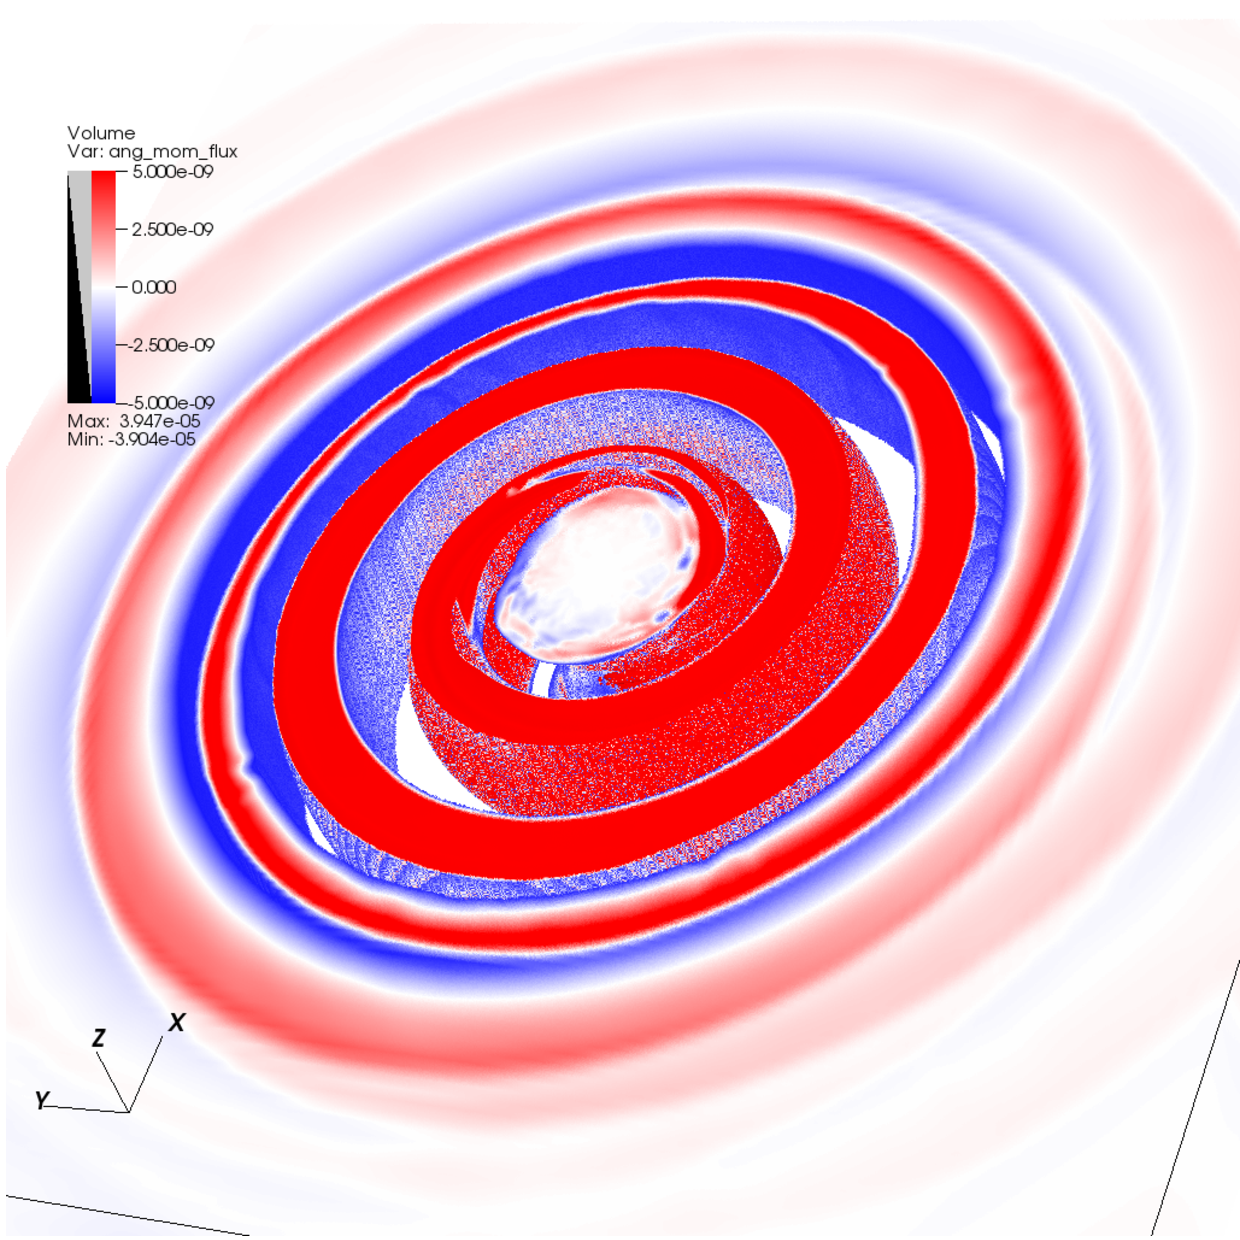
\includegraphics[width=0.49\textwidth]{raycasting_smooth_cropped.pdf}
    \caption{3D distribution of angular momentum density flux $J_r$
        from the DD2 simulation with turbulent viscosity at ${\sim}43.5$~ms after
        merger. $J_r$ is shown on a central region of
        $(89\times89\times60)$~km${}^3$ covering the remnant NS
        and disk, and it is given in units where $c=G=\Msun=1$.
        (Adapted from \citet{Nedora:2019jhl})
    }
    \label{fig:ang_mom_flux}
\end{figure}

\subsection{High mass ratio binaries}

Newly born \ac{MNS} is not axisymmetric. In addition to driving the angular 
momentum transport, it is a strong emittor of \acp{GW} at kiloHertz frequencies.
In ${\sim}10-20$~ms \pmerg{} the \acp{GW} remove about two time the 
amount of energy that was lost during the inspiral and merger \citep{Bernuzzi:2015opx}.
After that, the contribution of \acp{GW} to the system evolution, specifically to the angular momentum loss, drops \citep{Radice:2018xqa}. 
The long-term evolution, $\O(100)$~ms, of the remnant is driven primarely by the viscous processes and weak interactions.

After the emission of \acp{GW} subsides, the \acp{MNS} still have an excess in angular momentum and gravitational mass, with respect to the cold, rigidly rotating equilibrium with the same baryoinc mass \citep{Radice:2018xqa}.

The subsequent evolution of the \ac{MNS} is towards the axisymmetric configuration close to the mass-shedding limit. However, would a \ac{MNS} reach this state or collapse to a \ac{BH} depends on the details of \pmerg{} state and on the temperature and composition effects.


A subset of \ac{BNS} models with high mass-ratio forms a \ac{BH} 
during the merger \cite{Bernuzzi:2020txg}. The absence of the core bounce
is indicated by the monotonic increase of the central density.
Such a behavior is referred to as prompt collapse \citep{Radice:2020ddv,Bernuzzi:2020tgt,Bernuzzi:2020txg}.
Specifically, these are models with $q\gtrsim1.67$. 
\gray{During the merger, the companion star (less massive) undergoes a tidal disruption, as the tidal forces overcome the star's binding energy}. The star is then accreted onto the primary (most massive). 
The accretion raises its mass beyond the maximum supported limit by the \ac{EOS}, which leads to collapse. 
The newly formed \ac{BH} is surrounded by the accretion disk that was left from the tidally disrupted companion.

At formation, the disk has a large baryon mass, ${\sim}0.15\,\Msun$, in comparison with the disks formed in prompt collapse of equal mass binaries, \citep[\eg][]{Radice:2018pdn}. 
The disk is also neutron-rich $Y_e\sim 0.1$.

We show the evolution of the disk mass of several representative models in Fig.~\ref{fig:disk_mass_evo}.

\red{EJECTA to be moved to its own section}
The models that undergo the prompt collapse also eject matter on a dynamical timescale. The ejecta originates from tidal disruption of the compantion. It is neutron rich, confined largely to the orbital plane and exhibits a crescent-like azimuthal structure \citep{Bernuzzi:2020txg}.

\begin{figure}[t]
    \centering 
    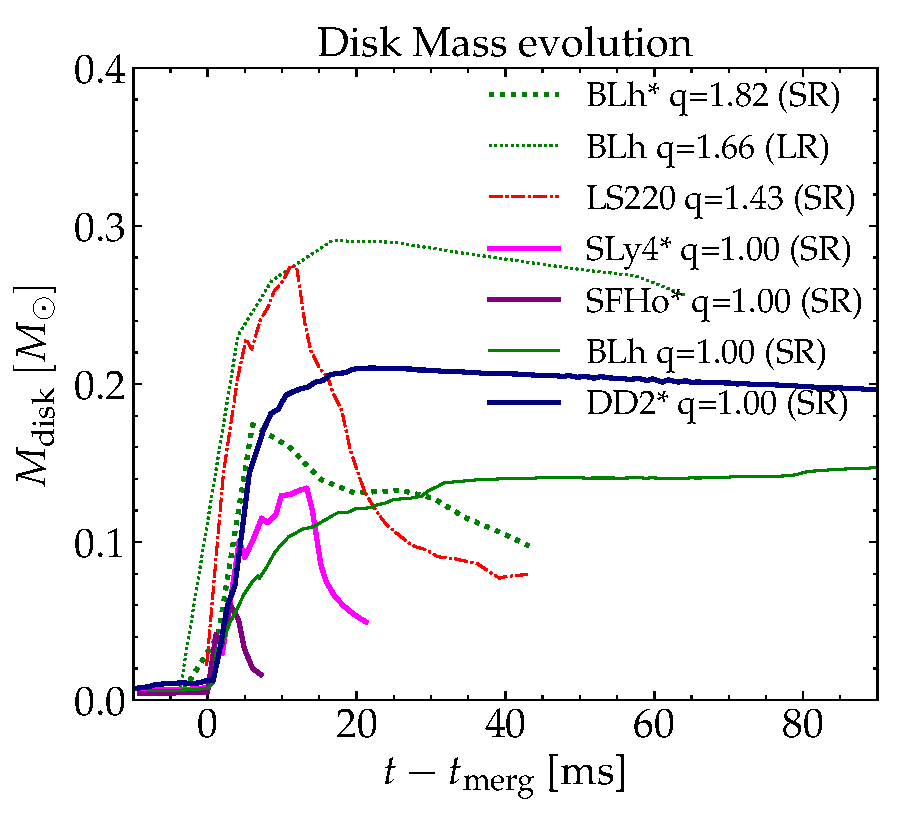
\includegraphics[width=0.49\textwidth]{disk/total_disk_mass_evo.pdf}
    \caption{Time evolution of the total disk mass for a few selected
        short-lived and long-lived cases. The former show a rapid 
        accretion right after disk formation. The plots show
        distinct difference in dynamical evolution after disk formation: accretion onto
        the newly formed BH (short-lived remnants) or accretion onto the NS
        remnant (DD2 $q=1$) with possible continuous mass shedding from the remnant
        into the disk (BLh* $q=1$). Adopted from \citet{Nedora:2020pak}
    } 
    \label{fig:disk_mass_evo}
\end{figure}


\subsubsection{Binaries with $q\lesssim1.4$}

Binaries with small mass ratio, ($q\lesssim1.4$) produce a \ac{MNS} remnant
that either survives on a dynamical timescale, set by the \ac{NS} rotation, before
collapsing to a \ac{BH}, or a \ac{MNS} that survives till the end of the simulations.
We refer to the former ones as \textit{short-lived} and the latter ones as 
\textit{long-lived} remnants.
Under the first category, fall the \ac{MNS} with relatively soft \ac{EOS}:
LS220 $q=1,1.1,1.2$, SFHo $q=1,1.1,1.4$ and SLy $q=1,1.1,1.4$. 
They collapse within $\sim20$~ms \pmerg. 
The exact time of the collapse however depends on the simulation resolution 
and on the inclusion of subgrid turbulence as was previosly noted by \citet{Radice:2017zta}.


\paragraph*{Disk of short-lived remnants}

During the merger, shocks generated at the collisional interface of the \acp{NS} cores,
as well as, tidal torques exerted by the non axisymmetric remnant result in a formation
of the disk. 
Matter, energy and angular momentum are injected into the disk as the spiral density waves 
propagate outwards from the mass-shedding \ac{MNS} remnant 
\citep{Bernuzzi:2015opx,Radice:2018xqa}.
\red{HERE the letter stuff could be added, actually}

%% --- Letter stuff
The spiral arms propagate from the remnant \ac{NS} into
the disk and transport angular momentum outwards as shown in
Fig.~\ref{fig:ang_mom_flux}. Such global density waves are a generic and
efficient mechanism to redistribute energy and eventually deplete  
accretion disks \citep{Goodman:2001a,Rafikov:2016a,Arzamasskiy:2018a}. 
%% Crucially, we find that both the $m=1$ and $m=2$ modes generate a \wind{} from the
%% disk's outer layers that is distinct from the dynamical ejecta, see Fig.~\ref{fig:ej_properties}.

Within these waves the fluid reaches highest temperatures, which decrease rapidly, as 
disk expansion and neutrino emission cools the matter. 
In such a high-temperature environment, the electron-positron pair creation is enhanced.
%% [added from Shibata Review paper]
As a result, neutrons can capture positrons $n+e^+p\rightarrow\bar{\nu}_e$.
The average particle energies are large, close to the mass difference between neutron 
and proton. 
In combination with the high $\nu_e$ and $\bar{\nu}_e$ luminosities,
the large number of available positrons leads to an increase 
in the fluid electron fraction, $Y_e$ from that of the initially neutron-rich material
\citep{Qian:1996xt}.
Additionally, a \ac{MNS} is a strong neutrino emitter. The neutrino irradiation of the 
surrounding area alters its composition, and neutrino absorption takes place
$n+\nu_e\rightarrow p + e^{-}$ and $p + \bar{\nu}_e\rightarrow n + e^+$.
This drives the neutron and proton fraction towards equilibrium, and raises the $Y_e$.
\red{paper says: 
    The electron fraction is reset by an initial excess of electron antineutrino emission
    and electron neutrino absorption,}
The entropy per baryon varies between $3$ and $\lesssim 10\,$$k_{B}$/baryon \citep{Perego:2019adq}.
%% ---
If \ac{MNS} remnant collapses to a BH, the main source of neutrinos shuts down and 
the inner part of the disk is rapidly accreted. 
The disk then approaches quasi-steady state, Fig.~\ref{fig:disk_mass_evo}, with 
axisymmetric, approximately Keplerian profile.
The inner part of the resulted disk, at densities $\rho\sim10^{13}$~\gcm, 
is relatively hot, $T\sim10\,$ MeV, but neutron-rich $Y_e\sim0.1$, as it was shielded 
from the neutrino irradiation. The disk gets progressively colder and proton-rich 
outwards with $Y_e$ reaching $0.4$ at the edges.
%% ---
The disk mass at formation appears to depend on the \ac{NS} \ac{EOS}. Binaries with 
stiffer EOS (larger \ac{NS} radii) produce more massive disk.
\red{[Fitting function]
    The disk mass can be described within the numerical uncertainties by a
    quadratic function of the mass ratio and the reduced tidal
    parameters (see Sec.~\ref{sec:remdisk}).}
Additionally, the disk mass show a dependency on mass ratio. For instance, the most massive disks are formed in LS220 $q=1.43$ and  BLh $q=1.82$ models, where the latter experiences prompt collapse.
%% -- 
The disk accretionon a \ac{BH} removes up to $50\%$ of the disk mass on a timescale tens of milliseconds.


\paragraph*{Disk of long-lived remnants}


If the \ac{MNS} is long-lived, the disk has time to complete its formation,
and thus it is more massive and extended \citep{Perego:2019adq}. 
As before, the disk is defined as matter, with $\rho\lesssim10^{13}$~\gcm. 
The disk mass increases with the mass ration and with stiffness of \ac{EOS}.
For instance, for BLh $q=1.00$ model, the disk mass reaches ${\lesssim}0.15\,\Msun$, 
while for DD2 $q=1.00$ model is exceeds ${\sim}0.2\,\Msun$.
For a models with BLh \ac{EOS}, the disk mass increases between $q=1.00$ and 
$q\sim1.4-1.5$ by a $100\%$.
%% ---
The long-term evolution of the disk is driven by its interaction with the \ac{MNS} 
remnant and cooling. 
And while in the case of a \ac{BH} remnant, the only possible interaction is the 
disk accretion onto a \ac{BH}, in case of a \ac{MNS} remnant the picture is more 
complex.
The disk neutrino cooling and gravitational pull from the remnant facilitates the 
accretion. However, generated at shocks, spiral density waves inject 
energy and angular momentum into the disk as well as centrifugally supported 
material (as \ac{MNS} undergoes mass-shedding). This heats up the disk and 
facilitates its expansion. 
In the figure  Fig.~\ref{fig:disk_mass_evo} the quasi-steady state disk accretion
is seen for the DD2 $q=1.00$ model. Meanwhile, in the BLh $q=1.00$ model, the 
mass-shedding by the remnant adds more material into the disk that it is being 
accretted. 
The analysis suggests, that this behaviour is due to two main factors: the 
very high average temperatures of the remnant and the disk achieved by this model, that 
are a consequence of the thermal effects included into the BLh EOS (\red{see sec.EOS}),
and the softness of the EOS, which lead to the strong oscillations of the 
remnant after merger (\red{see sec.DensyModes.}).

The inclusion of the subgrid turbulence smears the mass distribution of disk 
properties. The distributions of electron fraction, entropy per baryon and 
temperature appears broader. A more detailed quantitative analysis would require more 
simulations performed at several resolutions to disentangle the effects 
caused by the subgrid turbulence and by the finite grid \citep{Bernuzzi:2020txg,Radice:2020ids}.

\begin{figure}[t]
    \centering 
    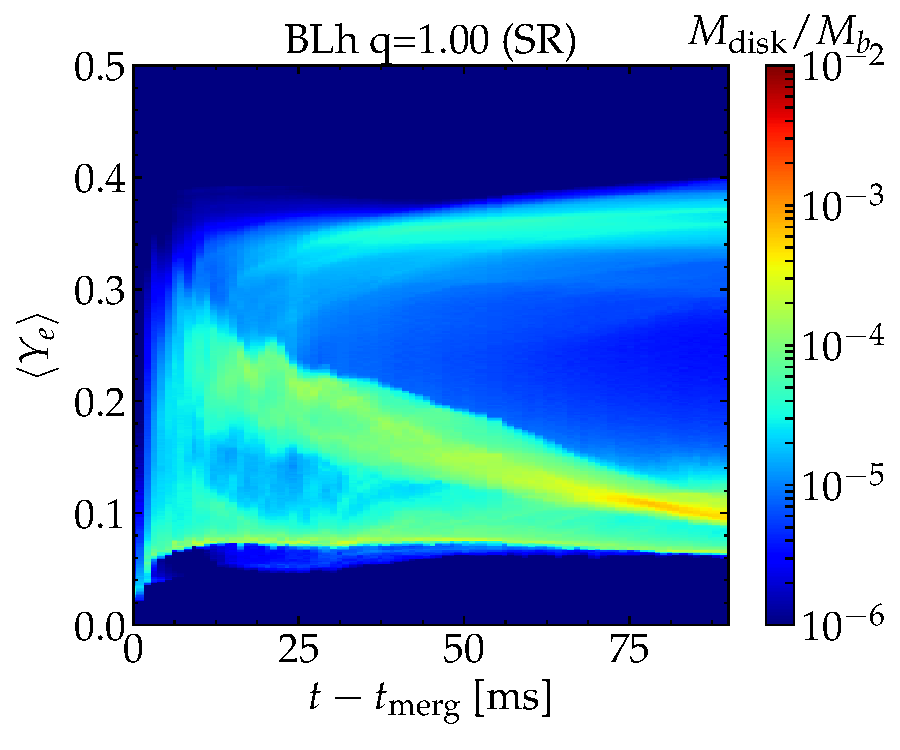
\includegraphics[width=0.49\textwidth]{disk/final_disk_timecorr_blh_q1_Lk.pdf}
    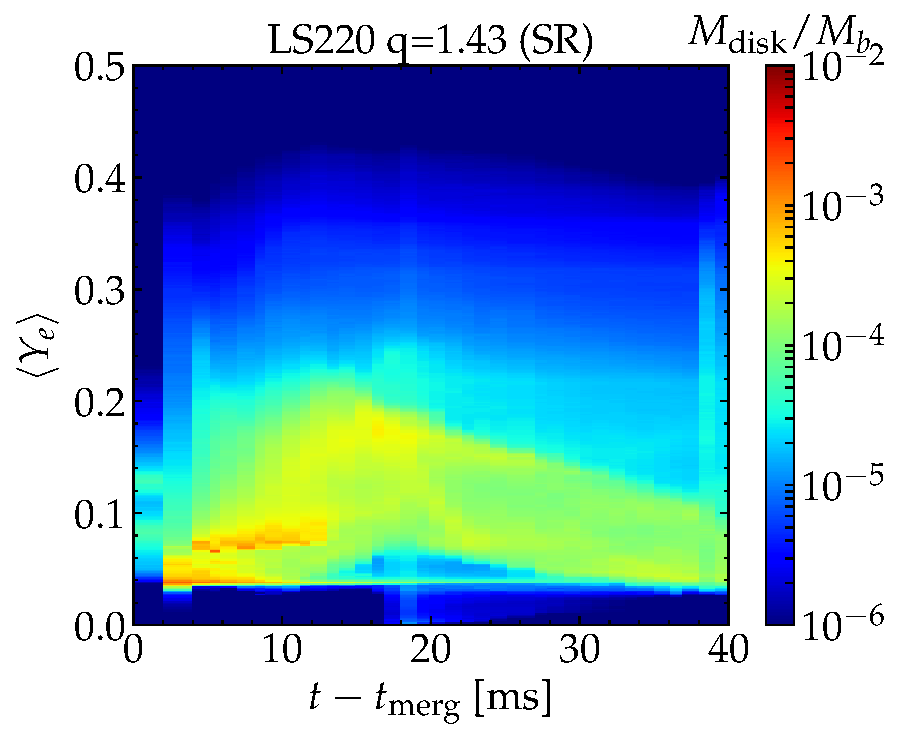
\includegraphics[width=0.49\textwidth]{disk/final_disk_timecorr_ls220_q14_LK.pdf}
    \caption{Evolution of the disk mass-averaged electron fraction with
        time for a long-lived (top) and a short-lived (bottom)
        remnant. The plot shows that with time the bulk of the disk lowers
        its $Y_e$ via cooling, while a small fraction in terms of mass
        gains a high $Y_e$, which relates to the highly 
        irradiated surface of the disk. Adopted from \citet{Nedora:2020pak}.
    }
    \label{fig:total_disk_time_corr_Ye_Blh_q1}
\end{figure}

\paragraph*{Evolution of disk properties}

%% Ye evolution
The evolution of the mass-weighted electron fraction for the model
BLh $q=1.00$, the model that is evolved till $\sim 90$~ms after merger, 
is shown on the top panel of Fig.~\ref{fig:total_disk_time_corr_Ye_Blh_q1}.
%% --- 
During the formation, shock and spiral waves raises the disk electron fraction to
$Y_e\sim0.25$. As the disk evolves, the bulk of its mass, shielded from neutrinos, 
(Fig. \ref{fig:slice:heating_hu}, density contours) 
returns to neutron-rich condition with $Y_e\lesssim0.1$. 
The outer part of the disk, however, is subjected to the 
strong neutrino irradiation and reaches $Y_e\sim0.4$ of a timescale of ${\sim}40$~ms.
%% Note that neutrinos in merger remnants decouple at $\rho\sim10^{11}$~$\gccm$ \citep{Endrizzi:2019trv}. 
Notably, the apparent gap in the $Y_e$ distribution if Fig.~\ref{fig:total_disk_time_corr_Ye_Blh_q1} at $\langle Y_e \rangle \simeq 0.15$ 
might not be of physical origin, but an artifact from the neutrino M0 scheme, 
that assumes neutrinos propagate along the radial directions
(see sec.NEUt.M0.SCHEME), that is not well suited for capturing the 
neutrino emission and reabsorption from the disk midplane.
%% ---
In case of a short-lived model LS220 $q=1.43$ model 
(lower panel of the Fig.~\ref{fig:total_disk_time_corr_Ye_Blh_q1})
the average electron fraction is lower, as there is no strong neutrino 
emitter. Additionally, the outskirts of the more compact disk remain 
at low electron fraction as the neutrino emitted by the disk itself 
are the only source of neutrinos. 

\paragraph*{Mass ejection on a long timescale}

As the disk expands and cools, the recombination of nucleons into 
alpha particles starts to take place.
The energy, released in recombination, might be sufficient for the outermost 
layers to become unbound, generating an outflow 
\citep{Beloborodov:2008nx,Lee:2009uc,Fernandez:2013tya}.
This processes however are expected to take place on a longer timescales,
that those that are simulated here.
On the $\sim100$~ms timescale, the outflows are driven by the neutrino heating, 
above the remnant, the so-called neutrino-driven wind 
(\nwind; \citealt{Dessart:2008zd,Perego:2014fma,Just:2014fka}),
and by the dynamical interactions between the \ac{MNS} 
remnant and the disk, the \swind{} \citep{Nedora:2019jhl}.
%% ---
We discuss the properties of the \nwind{} found in our simulations
in the section \red{sec.Ejecta.NuWind} and the properties of the 
\swind{} in the \red{sec.Ejecta.SWIND}.
%The \swind{} can have a mass up to
%a few $10^{-2}\,\Mo$ and velocities ${\sim}0.2$~c. The ejecta
%have electron fraction typically larger than ${\sim} 0.25$ since they are 
%partially reprocessed by hydrodynamic shocks in the expanding arms. 
%The \nwind{} is driven by neutrino heating above the remnant. It generates outflows
%with smaller masses ${\sim} 10^{-4}M_{\odot}$ and larger $Y_e$
%than the \swind{}. 
%Differently from \swind{} the mass flux of the \nwind{} in our simulations subsides 
%before the end of out simulations, due to rapid baryon loading of the 
%polar region.
%The \swind{} will be discussed in detail in Sec.~\ref{sec:spiralw}.
The effects of these outflows on the dynamical evolution of the remnant 
lies in the amount of mass and energy they can remove from the system.
Specifically, the \nwind{} have a typical mass of ${\sim} 10^{-4}\Msun$, 
while the \swind{} could remove $10^{-2}\,\Msun$ on a timescale of a $\sim100$~ms.

\begin{figure}[t]
    \centering 
    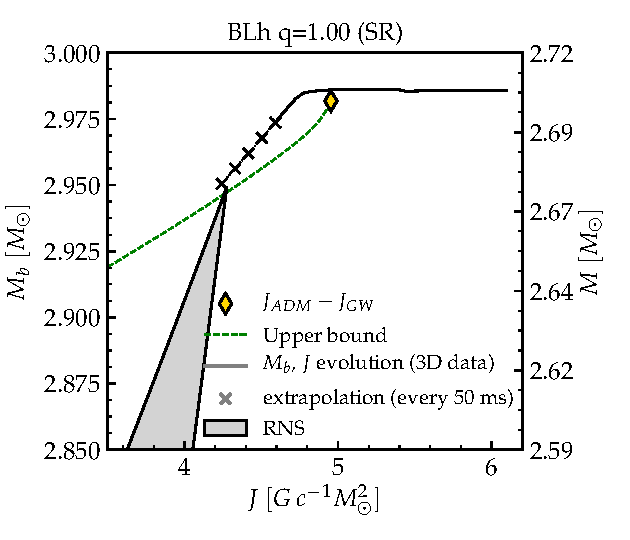
\includegraphics[width=0.49\textwidth]{ejecta_sec/secular_j_mb_RNS_blh.pdf}
    \caption{Baryon mass vs angular momentum diagram for the BLh $q=1$ remnant.
        The colored diamond marks the baryonic mass and angular momentum at the end
        of the dynamical gravitational-wave dominated phase.
        After the GW phase, the evolution is driven by the massive outflows.
        The solid black line is the $M_b$ and $J$ estimated from the 3D data
        integrals under the assumption of axisymmetry.
        The green dashed line is a conservative estimate
        of the mass ejection and a possible trajectory for the viscous
        evolution as estimated in \citet{Radice:2018xqa}. The crosses are
        a linear extrapolation in time of the solid black line. The gray
        shaded region is the region of stability of rigidly rotating NS equilibria.
        Adopted from \cite{Nedora:2020pak}
    }
    \label{fig:total_j_mb_rns_blh}
\end{figure}

To understand the remnant evolution on the timescales longer then the ones 
present here, requires ab-initio \ac{NR} simulations in $(3+1)D$ with compete physics.

Here we consider a BLh $q=1.00$ simulation, one of the longest runs we have performed.
After the merger, the \ac{MNS} remnant is born. With respect to the zero-temperature 
beta-equilibrium \ac{NS} configurations, the BLh $q=1.00$ 
remnant has an excess in baryon mass.
In the figure~\ref{fig:total_j_mb_rns_blh} we show the evolution of the 
total baryon mass, $M_b$, and total angular momentum, $J$, of the remnant.
As the total baryon mass is conserved (if there is no outflow), the early evolution 
of the remnant proceeds with $M_b=\text{const}$. The angular momentum is however 
lost by the remnant to emission of \acp{GW}. 
We evaluate the amount of angular momentum lost to \acp{GW} following the 
\citet{Damour:2011fu,Bernuzzi:2012ci,Bernuzzi:2015rla}.
\red{This has to be defined and noted that we use $\sim20$~ms postmerger mark
    and how exactly we compute all of it, the David's script
}
Substruct it from the initial data \ac{ADM} angular momentum we obtain the value 
that is left to the system after the \ac{GW} phase 
(the yellow marker on the Fig.~\ref{fig:total_j_mb_rns_blh}).
%% ---
Notably, after the \ac{GW} phase, the remnant still has an excess in angular momentum
in comparison with the rigidly rotating \ac{NS} configurations with the same baryon mass 
(gray triangular region in Fig.~\ref{fig:total_j_mb_rns_blh}).
We observe the same situation across all models \citep{Zappa:2017xba,Radice:2018xqa}.
\gray{
    On the angular momentum estimation:
    The radiated angular momentum (as well as energy) are computed from the 
    multipole loments $N_{lm}$ for the \ac{NR} complex "news function" at infinity. 
    The $J_{z;\text{rad}}(t)$ is computed as \citep{Damour:2011fu} 
    \begin{equation}
    \Delta J_{z\text{rad}}(t) \frac{1}{16}\sum_{l,m}^{l_{max}}\int_{t_0}^{t} dt' m \mathcal{L}[h_{lm}(t')(N_{lm}(t'))^*],
    \end{equation}
    where $h_{lm}$ is the multipolar metric waveform, 
    $N_{lm}(t) = dh_{lm}(t) / dt$, the news function, and $l_{max}=8$.
    The $J$ loss is metric dependent ($h$).
    The $h$ (strain???) is computed from $\Psi_4(t) = dN/dt = d^2h/dt^2$ by a 
    frequency-domain integration procedure with a low-frequency cut 
    $\omega_0 = 0.032/(m_1+m_2)$.
}
%% ---
The baryon mass of the remnant also exceeds maximum mass that a rigidly rotating 
equilibria could have.
Such remnant is generally referred to as a hypermassive neutron star (HMNS) following the 
nomenclature introduced for zero-temperature EOS equilibria \acp{NS} \citep{Baumgarte:1999cq}.
Such a remnant is expected to collapse to a BH. 
%% ---
However, a remnant can avoid the collapse by efficiently removing angular momentum
and mass and entering the rigidly rotating equilibria zone. 
%% ---
We compute the angular momentum and baryon mas evolution of the remnant, 
through volume integrals, assuming axisymmetry and evaluating the former using Eq.~\eqref{eq:method:ang_mom}, and the latter using the Eq.~\eqref{eq:method:mdisk}. 
The evolution of these two quantities is depicted with the black solid line if 
Fig.~\eqref{fig:total_j_mb_rns_blh}~\footnote{Note that the angular momentum estimated
    from the GW and from the integral of Eq.~\eqref{eq:method:ang_mom} assuming
    axisymmetry are compatible within the errors made in the latter estimate.
}.
We observed that after the \ac{GW} phase, the remnant continues to evolve, loosing the 
angular momentum together with the baryon mass. This is achieved through massive outflow,
the \swind{}. 
The extrapolation of the final trend of the mass and angular momentum loss shows, that 
if $\approx0.05\,\Msun$ ($\approx40$\% of the final disk at the end of simulation) is 
ejected, the \ac{MNS} remnant would approach the rigidly rotating equilibria region 
at the mass-shedding limit. Extrapolation indicates, that if the ejecta mass flux does 
not change, this would occur on a timescale of $\sim 300$~ms \pmerg{}.
Similar results are obtained with the conservative upper bound estimate on the 
evolution of the long-lived remnant (Eq.~$2$ in \citet{Radice:2018xqa}) (green dashed line in figure).
\red{WHAT the fuck is Keplerian limit, mass-shedding limit and rigidly rotating equilibria}
Additionally, while this simulation included the effects of turbulent viscosity on the
angular momentum transport, the ejecta could be further enhanced by the magnetic stresses 
\citep{Metzger:2006mw,Bucciantini:2011kx,Siegel:2017nub,Fernandez:2018kax,Ciolfi:2020hgg}.

Other simulations also produce a \ac{MNS} remnant with a similar evolutionary path. 
Models with DD2 \ac{EOS} however, are born with an excess in angular momentum, but not in 
baryon mass. They also evolve toward the rigidly rotating equilibria but slower.
Models with $q>1.00$ produce remnants that generally have larger excess in angular momentum 
and mass have how to shed a larger amount of mas to reach equilibrium configuration.
(\red{However we also show that these models tend to have stronger \swind{}, see sec.SPIRAL.WIND})
Overall, we estimate that for models with $q=1.00$ need to shed ${\sim}0.05\Msun$ while 
models with $q\eqsim 1.4$ need to remove $0.2\Msun$ to reach equilibrium configuration.



\section{Mass ejection in \ac{BNS} merger simulations}

%% \section{Results -- Mass Ejection}


Tidal interactions and shocks exerted on the \acp{NS} at merger trigger the ejection of material
on the dynamical timescale. This is the \ac{DE} \citep[\eg][]{Hotokezaka:2013b,Bauswein:2013yna,Radice:2016dwd,Radice:2018pdn}. 



\subsection{Dynamical Ejecta}


%% The mechanism behind the dynamical ejecta [radice:2018pnd]
Tidal interactions and shocks exerted on the \acp{NS} at merger trigger the ejection of material
on the dynamical timescale. This is the \ac{DE} \citep[\eg][]{Hotokezaka:2013b,Bauswein:2013yna,Radice:2016dwd,Radice:2018pdn}. 

\red{More on the genral mechanism tidal vs shocked}
The \ac{DE} is evaluated with the geodesic criterion introduced in Sec.~\ref{sec:method:analysis:ejecta}.

Describe shock vs tidal components 

\subsubsection{Overall properties of the \ac{DE}}


The novelty of the set of models discussed in this thesis with respect to the 
previous study by \citet{Radice:2018pdn} is that all models include the neutrino heating via M0 scheme 
(see Sec.\ref{sec:theory:neutrino}) in addition to the neutrino cooling and for most models the effects 
of subgrid turbulence (see Set.\ref{sec:theory:grles}) are included.
Meanwhile, models cover a significantly more narrow range in 
dimensionless tidal deformability, $\tilde{\Lambda}$, and mass ratio, motivated by the \GW{}.

We can qulitativly asses the effects of neutrino heating by comparing the overall properties 
of our model set and that of the \citet{Radice:2018pdn}.
Specifically, the neutrino absorption leads to not only an increase in average electron 
fraction but also to larger total ejected mass and velocity. The latter two would be 
crucial for the non-thermal, kilonova afterglow (see Sec.\red{sec:KilonovaAfterglow}).

The mass averaged over the simulations from Tab.~\ref{tab:sim} is 
$\overline{\amd} = (3.442 \pm 2.495)\times 10^{-3}\,M_{\odot}$ (where
hereafter we report also the standard deviation), while the same
quantity calculated for data of \cite{Radice:2018pdn} 
is $\overline{\md} = (1.352\pm 1.250)\times 10^{-3}\,\Msun$.
The mass-averaged terminal velocity of the dynamical ejecta 
ranges between $0.1$c and $0.3$c, and in a good agreement with 
\cite{Radice:2018pdn}.
The mass-averaged velocity, averaged over all the simulations, is 
$\overline{\avd} = (0.172\pm0.038)\,{\text{c}}$.

We find that in our set of models, there is a correlation of $\avd$ with the tidal parameter 
$\tilde{\Lambda}$: the higher the $\tilde{\Lambda}$ the lower the $\avd$.
This can be understood from the general mechanism of the \ac{DE},
that tells in mergers of binaries with $q=1.00$, the shocked component of the ejecta 
is the dominant. The strength of shocks increases as the \acp{NS} become more compact 
(with decreasing $\tilde{\Lambda}$) and hence collide at higher velocities~\footnote{Note that in the definition of prompt collapse we adopted, there is no shocked ejecta.}.
%% ---
For binaries with high mass ration, however, the tidal component of the \ac{DE} is dominant. 
The velocity of the latter also is smaller for larger $\tilde{\Lambda}$, as stars collide 
at slower velocities due to their larger radii. 
%% ---
The mass-averaged electron fraction, $\ayd$, of our models lies the range $(0.1, 0.3)$
with an averaged value among all models $\overline{\ayd} = 0.175 \pm 0.063$.
Notably, the \citet{Radice:2018pdn} reported a more narrow range, $(0.1, 0.2)$.
This is a clear effect of the neutrino absorption included in our models, that elevates 
the everal electron fraction of the \ac{DE} as it is being irradiated by neutrinos 
during the merger.
Notably, the $\ayd$ of our models is close to those obtained with M1 
scheme of \citet{Sekiguchi:2016bjd} and \citet{Vincent:2019kor}.
%% ---
The effect of subgrid turbulence on the dynamical ejecta properties however,
found rather week and comparible to the effects of finite grid distritization 
\citep{Bernuzzi:2020txg,Radice:2020ids}.

We find that the properties of the \ac{DE} depends on the \mr{} and on the 
\ac{EOS} softness that can be parameterized with $\tilde{\Lambda}$. 
We investigate in detail the statistical properties of our set of models as well as 
other \ac{NR} \ac{BNS} data sets available in the literature in 
section \ref{sec:ejecta_disk_statisitcs}.
\red{Link to the fitting data}



\subsection{Fast tail of the dynamical ejecta}
\red{To be filled when the Afterglow paper is on arxive}

%\begin{figure}[t]
%    \centering 
%    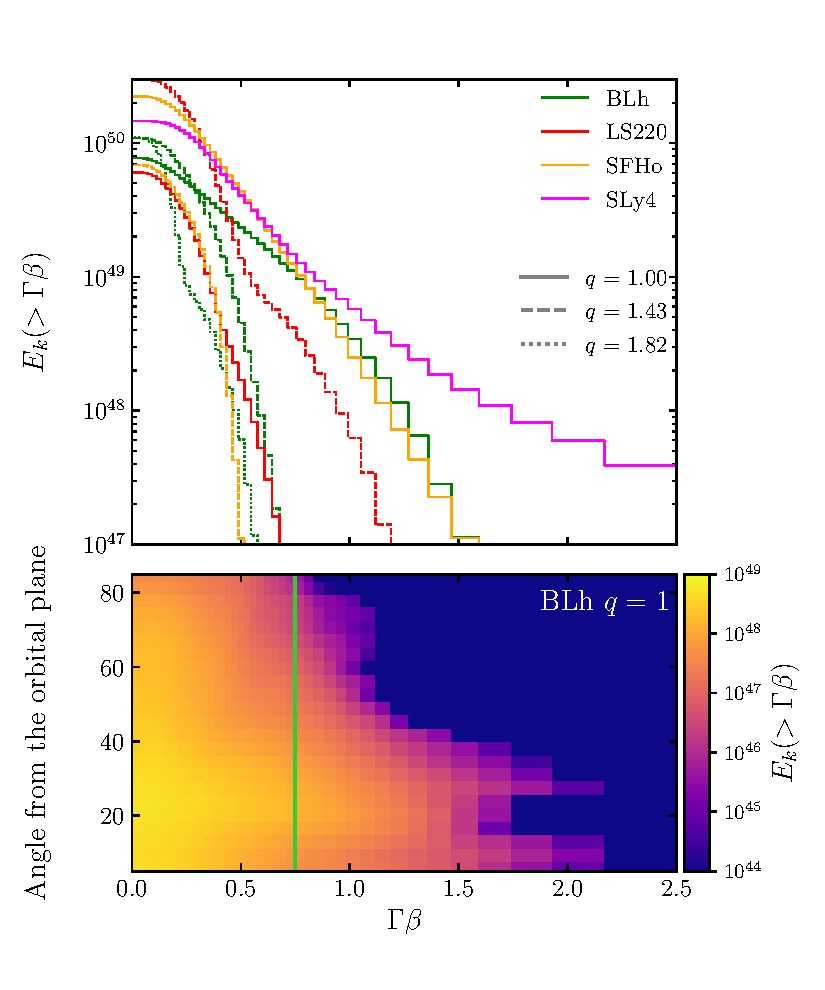
\includegraphics[width=0.49\textwidth]{./figs/kinetic_energy_struct_models.pdf}
%    \caption{
%        Total kinetic energy distribution for a selected set of models (\textit{top panel}) 
%        and angular distribution of kinetic energy for a BLh $q=1.00$ model (\textit{bottom panel}).
%        %% Also shown as a solid black line is the slow quasi-spherical model of \cite{Mooley:2017enz}.
%        The vertical light green line marks the $\upsilon_{\text{ej}}=0.6$.
%        The top panel shows that equal mass models have a more extend high energy tail,
%        while the bottom panel shows that the angular distribution of the ejecta is not 
%        uniform.
%        \red{Adopted from Nedora et al. (2021)}
%    } 
%    \label{fig:ejecta_vel_hist}
%\end{figure}
%
%The velocity distribution of \ac{DE} was found to include a very fast, 
%$\upsilon_{\text{ej}}\geq0.6$~c tail
%\cite{Piran:2012wd,Hotokezaka:2013b,Kyutoku:2012fv,Ishii:2018yjg,Hotokezaka:2018gmo,Radice:2018pdn}.
%%% ---
%The total mass of this tail was found to be dependent on the
%binary parameters and solution resolution,
%with an average $\sim 10^{-6}-10^{-5} M_{\odot}$.
%%% ---
%With respect to the fast tail origin, it can be divided into two main components 
%\citep{Radice:2018pdn}.
%The early component, that comprises the ejecta that is generated at the collisional interface 
%of two \acp{NS} of similar mass and directed primarily along the binary axes.
%And the late component that consist of matter that driven by the shock breakout from the ejecta 
%after the core bounce and confined mostly to the binary plane. 
%
%Among the simulations listed in \ref{tab:sim}, we select \red{XX} simulations 
%performed at standard resolution, and for which fast ejecta is found.
%%% ---
%Here we extract ejecta properties at the detector located at 
%$R=300G/c^2M_{\odot}\approxeq443$~km, from the merger, in agreement with \citet{Radice:2018pdn}.
%
%The mean value of the fast tail mass is
%
%\be\label{eq:ejecta:dyn:avg:M}
%\red{ \overline{\amd}(\upsilon>0.6) = (2.50 \pm 4.23)\times 10^{-5}M_{\odot}\ , }
%\ee
%
%where the standard deviation is also reported as an error.


%% ------------------ 
%% Note that the geodesic criterion above neglects the fluid's pressure and might
%% underestimate the ejecta mass. The Bernoulli criterion assumes that the (test
%% fluid) flow is stationary, so that there is a pressure gradient that can
%% further push the ejecta.  We find that both criteria predict dynamical
%% ejecta masses that are practically indistiguishable and well within the numerical uncertainties \citep{Bernuzzi:2020txg} if applied to extraction spheres at large coordinate radii; 
%% differences between the two criteria are instead present if they are applied to
%% matter volumes \citep[cf.][]{Kastaun:2014fna}.


\subsection{Spiral-wave wind}

\label{sec:spiralw}


\begin{figure*}[t]
    \centering 
    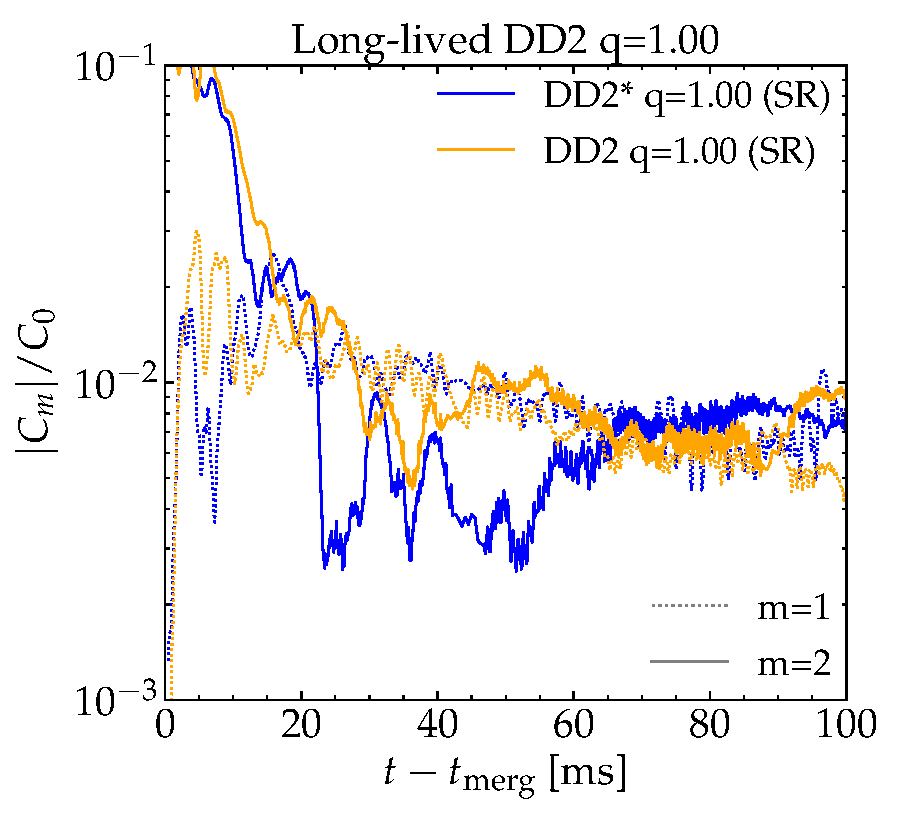
\includegraphics[width=0.49\textwidth]{remnant/dens_modes/modes_rho_dd2.pdf}
    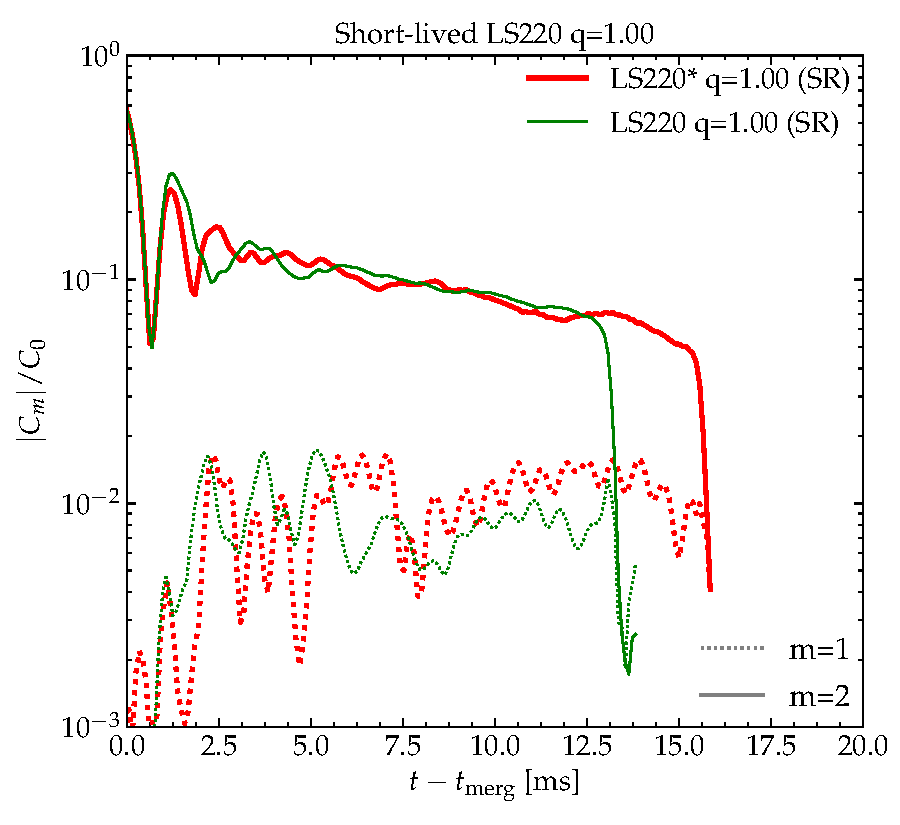
\includegraphics[width=0.49\textwidth]{remnant/dens_modes/modes_rho_ls220.pdf}
    \caption{Modes analysis for exemplary equal-mass long-live and short-lived
        remnants. The evolution of the $m=2$ and the $m=1$ monitored by
        Eq.~\eqref{eq:modes} is shown for the DD2 and LS220 remnant with and
        without turbulent viscosity. The $m=2$ mode in the long-lived
        remnant is strongly damped by the emission of gravitational
        radiation and becomes comparable to the $m=1$ mode on a timescale of
        ${\gtrsim}20\,$ms. Turbulent viscosity sustain the $m=2$ mode for
        a longer period. The $m=2$ mode is instead dominant to collapse in
        the short-lived remnant.
        (Adopted from \cite{Nedora:2020pak})
    }
    \label{fig:dens_modes}
\end{figure*}

Here we discuss the dynamics of spiral waves and the associated outflow, the \ac{SWW}.


\subsubsection{Remnant \& disk dynamics}


The hydrodynamical modes of the \ac{MNS} remnant are computed following the 
method described in Sec.\ref{sec:method:HDmodes}. 
The mode analysis is shown in the Fig.\ref{fig:dens_modes} for two representative 
simulations, the short-lived LS220 $q=1.00$ and the long-lived DD2 $q=1.00$.
The newly born \ac{MNS} remnant is not axisymmetric, displaying characteristic 
spiral arms, extending outwards from the shock interface of the collided cores 
\citep{Shibata:1999wm,Shibata:2006nm,Bernuzzi:2013rza,Kastaun:2014fna,East:2015vix,Paschalidis:2015mla,Radice:2016gym,Lehner:2016wjg}.
The bar-shaped, $m=2$ modes is the dominant one early in \pmerg{}, while the 
one-armed spiral $m=1$ modes stars to dominate in the late evolution 
\citep{East:2015vix,Paschalidis:2015mla,Radice:2016gym,Lehner:2016wjg,Bernuzzi:2013rza,Kastaun:2014fna}.
Indeed, the $m=2$ mode remains the dominant one until $\sim15-20$~ms \pmerg{}. 
After that, the LS220 $q=1.00$ model forms a \ac{BH}. 
In the DD2 $q=1.00$ model, however, the $m=1$ mode becomes comparable with $m=1$ 
throughout the remainder of the evolution, while the $m=2$ mode efficiently dissipates 
through \ac{GW} emission \citep{Bernuzzi:2015opx,Radice:2016gym}.
%% ---
We find that the magnitude of the $m=1$ mode increases with the binary \mr{}.
For instance the largest $C_{m=1}$ are found in BLh $q=1.43$ and LS220 $q=1.22$.
Stronger $m=1$ leads to more large \ac{SWW} mass flux.
The dependency of the $C_{m=2}$ on \mr{} however is not clear. 
This is in agreement with what reported by \citet{Lehner:2016wjg}.

Formation of the spiral arms is a generic hydrodynamic effect, that was identified 
in the \ac{NR} simulations with polytropic \ac{EOS} 
\citep{Bernuzzi:2013rza,Radice:2016gym}.
However, the evolution of these arms and quantitative behaviour of hydrodynamic
modes depends on the physics input. 
In the Fig.~\ref{fig:dens_modes} we show that the turbulent viscosity in the 
DD2 $q=1.00$ remnant stabilizes the $m=2$ mode, enhancing the angular momentum 
transport into the disk.
The $m=2$ mode, however, remains largely unaffected by the turbulent viscosity.
Similarly, the models' evolution in the LS220 $q=1.00$ is too short, for the 
subgrid turbulence to become important.

We compute the angular momentum of the \ac{MNS} remnant following the method,
discussed in Sec.\ref{sec:method:angmom}, where the remnant is distinguished 
from the disk on the basis of the rest mass density $\rho=10^{13}$~\gcm{} 
(see Sec.\ref{sec:method:diskdef}).
We find that for a long-lived rmnant 
on a timescale of $\sim20$~ms, about half of the total angular momentum 
of the \ac{MNS} remnant is transferred into the disk. 
%% [ from shibata review ]
This is a consequence of the fact that the remnant \ac{MNS} is strongly deformed 
after merger and gravitational torque on the surrounding matter, 
that allows for a rapid angular momentum transport.
%% ---
After, the remnant settles on quasi-stationary evolution path 
(see Sec.~\ref{sec:bns_dynsmics_overview}).

Following the disk and remnant mass evolution we observe, that the spiral 
density modes inject ${\sim}0.1-0.4\,\Msun$ of baryon mass into the disk during the 
first ${\sim}20$ms. 
The mass injection appears to be stronger for stiffer \acp{EOS}. 
With respect to the \mr{}, the higher $q$ binaries form a larger disc 
(see BLh* $q=1.82$ and LS220* $q=1.43$ on the Fig.~\ref{fig:disk_mass_evo}).

\begin{figure}[t]
    \centering 
    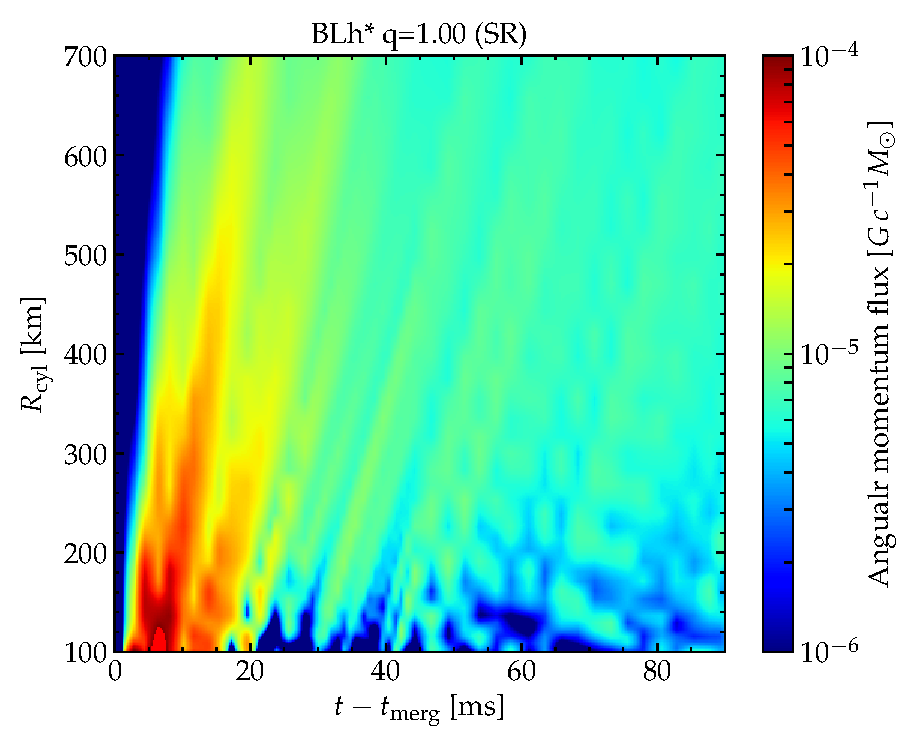
\includegraphics[width=0.49\textwidth]{remnant/evol_jflux_2d_BLh_M13651365_M0_SR_R1.pdf}
    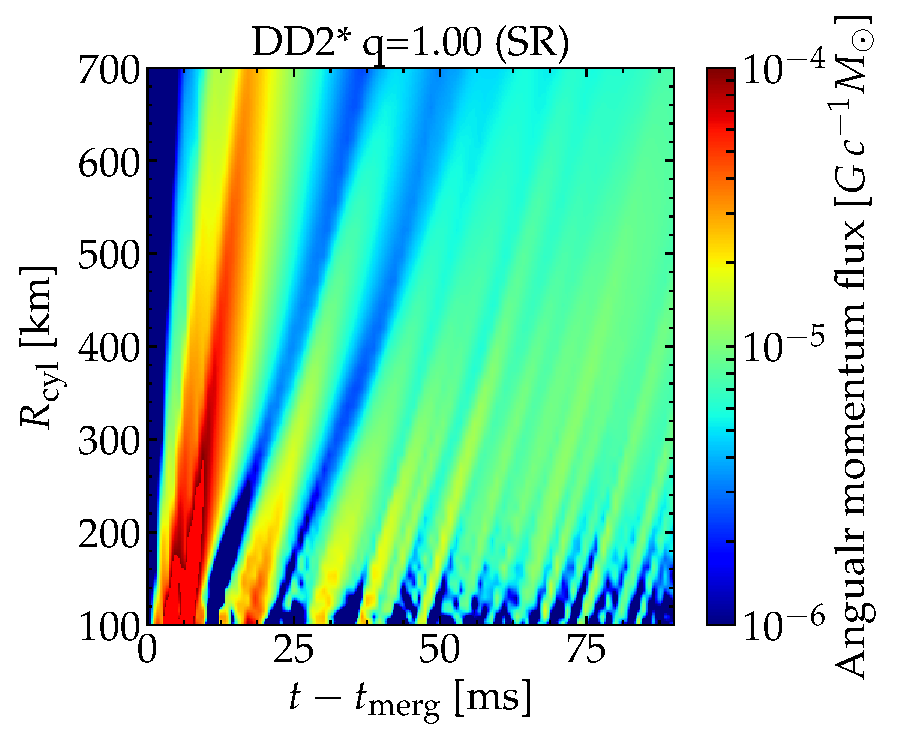
\includegraphics[width=0.49\textwidth]{remnant/evol_jflux_2d_DD2_M13641364_M0_SR_R1.pdf}
    \caption{Angular momentum flux through consecutive cylindrical
        surfaces identified by cylindrical radii from $R_{\text{cyl}}=100$ to $R_{\text{cyl}}=500$. The
        plot shows the angular momentum transport into the disk.
        Adapted from \citet{Nedora:2020pak}
    }
    \label{fig:disk_ang_mom_flux_map_blh_q1}
\end{figure}

In the Fig.~\ref{fig:disk_ang_mom_flux_map_blh_q1} we show how the 
angular momentum is being transported from the \ac{MNS} remnant into the disk
in two long-lived models with turbulent viscosity, DD2* $q=1.00$ and BLh $q=1.00$.
The angular momentum is transported via spiral waves that correspond do the 
hydrodynamic models, $m=1$ and $m=2$ discussed above.
We observer, that in the model with more stiff DD2 \ac{EOS},
the fist wave is stronger. Notably, the DD2* $q=1.00$ model 
also has a more massive disk.
%% --- 
Further, the evolution of the disk-remnant interactions 
after $\sim20$~ms \pmerg{} is different for two models. 
While the model with DD2 \ac{EOS} stops shedding mass into 
its disk and starts slowly accreting, the model with BLh \ac{EOS} continues to shed mass into the disk
(see Fig.~\ref{fig:disk_mass_evo} and discussion in
Sec.~\ref{sec:bns_dynsmics_overview})
The latter is caused by the strong angular momentum flux \red{actually the plot shows, that it is not}, emanating 
from the \ac{MNS} remnant and by the larger temperatures, 
that reached in the model with the BLh \ac{EOS}.
Larger temperatures leads to lower rotational frequency 
at which the mass shedding occurs \citep{Kaplan:2013wra}. 

The subgrid turbulence enhances the angular momentum transport. However more simulations of long-lived 
\ac{MNS} remnants are needed to asses the effects of the 
subgrid turbulence and \mr{} systematically. 

\begin{figure}[t]
    \centering 
    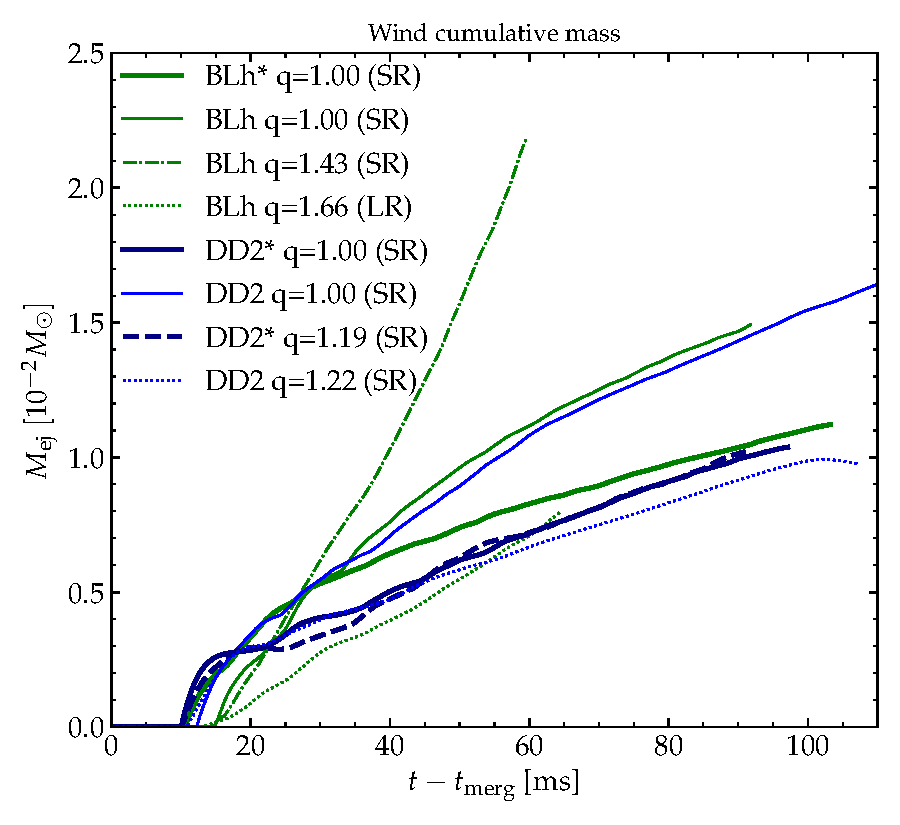
\includegraphics[width=0.50\textwidth]{ejecta_postdyn/wind_mass_flux.pdf}
    \caption{Cumulative mass of the \swind{} from long-lived
        remnants. The wind persists on timescales of $\O(100)\,$~ms with
        mass fluxes ${\sim}0.33-1.23\,\Msun/s$.
        Adapted from \citet{Nedora:2020pak}.
    }
    \label{fig:mej:bern}
\end{figure}

\begin{figure*}[t]
    \centering 
    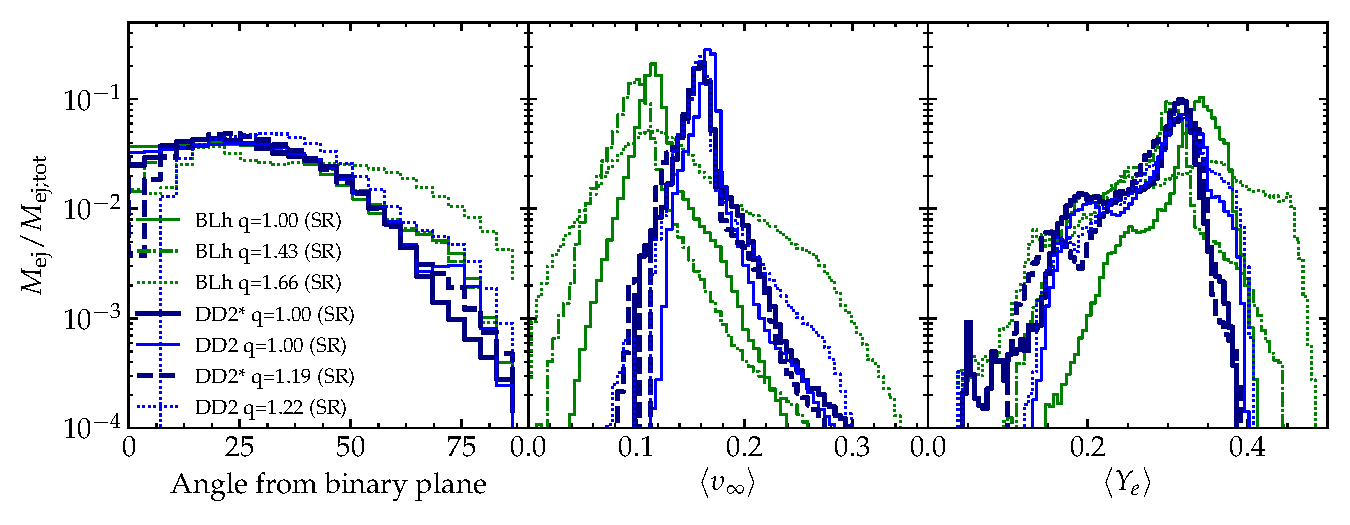
\includegraphics[width=0.99\textwidth]{ejecta_postdyn/wind_hists_shared.pdf}
    \caption{Mass-averaged histograms of the \swind{} for a selected
        subset of long-lived remnant. From left to right: ejecta angular
        distribution, ejecta terminal velocity and electron
        fraction. Remnants from more asymmetric binaries produce winds
        with broader angular distribution.
        The \swind{} from the DD2 EOS remnants has larger velocities
        then the winds from the softer BLh EOS. The electron fraction
        peaks at ${\sim}0.3$ and it is distributed from $0.1$ to $0.4$.
        Adapted from \citet{Nedora:2020pak}.
    }
    %
    \label{fig:ejecta:bern:hist}
\end{figure*}

\begin{figure}[t]
    \centering
    %% 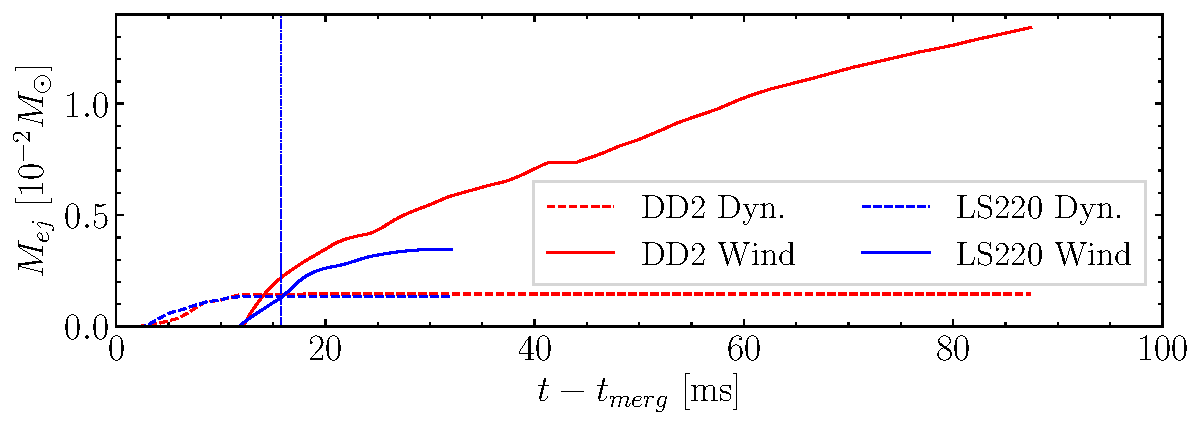
\includegraphics[width=0.49\textwidth]{ejecta_postdyn/ejecta_profiles_dd2_ls220_long.pdf}
    %% 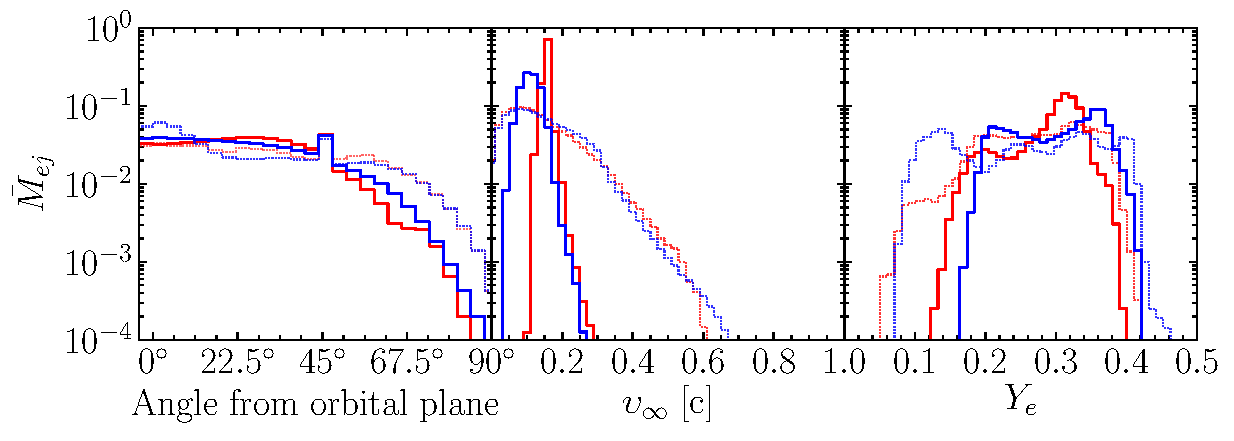
\includegraphics[width=0.49\textwidth]{ejecta_postdyn/hist_1D_dd2_ls220_long.pdf}
    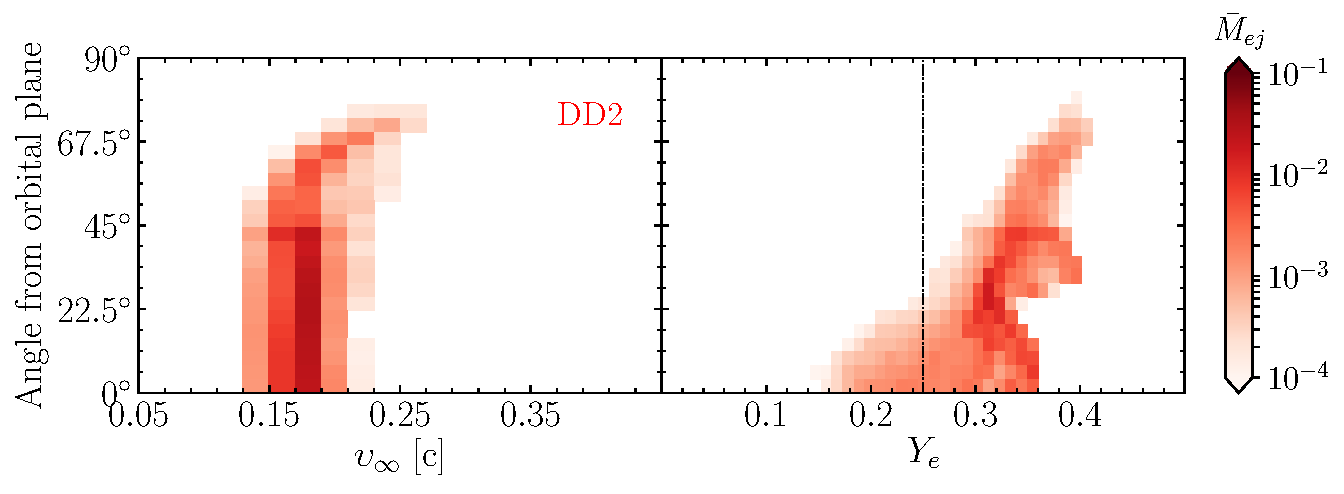
\includegraphics[width=0.99\textwidth]{ejecta_postdyn/corr_dd2.pdf}
    \caption{Properties of the \ac{SWW} and dynamical ejecta
        computed form the simulations with turbulent viscosity.
        %
        Top: evolution of unbound mass for dynamical ejecta
        (dashed lines)
        and \ac{SWW}
        (solid lines). $t=0$ marks the moment of merger, the vertical
        line marks the collapse time of the LS220 BNS.
        %
        Middle: mass histograms for the angular (left), velocity (center) and electron
        fraction (right) distributions.
        Bottom: angular distribution and composition of the \ac{SWW}
        for DD2.
        %
        Note the $\bar{M}_{ej}$ in the middle and bottom panels is normalized to one.
        (Adapted from \citet{Nedora:2019jhl})
    }
    \label{fig:ej_properties}
    
\end{figure}

%% --------------------------------
%% TAB WIND SUMMARY
\begin{sidewaystable}
%\begin{table*}[t]
  \centering
  \captionsetup{width=1.0\linewidth}
  \caption{%
    Summary table of the \swind{} properties of long-lived remnants. The columns contain
    the following information, starting from the left. Equation of
    state, mass-ratio, available resolutions,
    inclusion of subgrid turbulence, time of the
    simulation end, mass of the
    \swind{}, mass-loss rate via \swind, mass-averaged electron fracton, terminal
    velocity and, finally, RMS angle for \swind{}. For these four
    quantities we give the mean value among the resolutions and
    one-sigma deviations. For binaries for which only one
    resolution is present, the error is assumed to be $20\%$ of the value.
    (Adapted from \cite{Nedora:2020pak}).
    }
  \label{tab:spiralwavewind}
  \begin{tabular}{c c c c c c c c c c}
    \hline\hline
    EOS & $q$ & Resolution & GRLES & $t_{\text{end}}$ & $\amw$ & $\amw/\Delta t$ & $\ayw$ & $\avw$ & $\langle \theta_{\text{ej}}^{\text{w}} \rangle$ \\
    &   &   &   & [ms] & $[10^{-2} M_{\odot}]$ & $[M_{\odot}/s]$ &   & $[c]$ &   \\ 
    \hline
    \hline
    BLh & 1.00 & \texttt{SR HR LR} & \cmark & $43.3$ $91.8$ $23.1$ & $0.39^{+0.07} _{-0.07} $ & $0.70^{+0.32} _{-0.32} $ & $0.31^{+0.01} _{-0.01} $ & $0.12^{+0.01} _{-0.01} $ & $27.06^{+2.61} _{-2.61} $ \\
    BLh & 1.00 & \texttt{SR} & \xmark & $ $ $103.2$ $ $ & $1.12^{+0.57} _{-0.57} $ & $1.07^{+0.21} _{-0.21} $ & $0.34^{+0.01} _{-0.01} $ & $0.12^{+0.02} _{-0.02} $ & $15.72^{+2.00} _{-2.00} $ \\
    \hline
    BLh & 1.18 & \texttt{LR} & \cmark & $69.4$ $ $ $ $ & $1.28^{+0.64} _{-0.64} $ & $1.23^{+0.25} _{-0.25} $ & $0.33^{+0.01} _{-0.01} $ & $0.11^{+0.02} _{-0.02} $ & $14.98^{+2.00} _{-2.00} $ \\
    \hline
    BLh & 1.43 & \texttt{LR SR} & \cmark & $35.1$ $59.6$ $ $ & $0.75^{+0.18} _{-0.18} $ & $1.06^{+0.67} _{-0.67} $ & $0.27^{+0.01} _{-0.01} $ & $0.09^{+0.01} _{-0.01} $ & $19.43^{+2.22} _{-2.22} $ \\
    \hline
    BLh & 1.54 & \texttt{LR} & \cmark & $45.8$ $ $ $ $ & $0.63^{+0.32} _{-0.32} $ & $0.44^{+0.09} _{-0.09} $ & $0.32^{+0.01} _{-0.01} $ & $0.10^{+0.02} _{-0.02} $ & $21.46^{+2.00} _{-2.00} $ \\
    \hline
    BLh & 1.66 & \texttt{LR SR} & \cmark & $64.6$ $20.1$ $ $ & $0.12^{+0.09} _{-0.09} $ & $0.37^{+0.34} _{-0.34} $ & $0.33^{+0.05} _{-0.05} $ & $0.13^{+0.01} _{-0.01} $ & $52.08^{+20.89} _{-20.89} $ \\
    \hline
    \hline
    DD2 & 1.00 & \texttt{LR SR HR} & \cmark & $123.0$ $113.0$ $74.4$ & $1.25^{+0.14} _{-0.14} $ & $1.30^{+0.19} _{-0.19} $ & $0.30^{+0.01} _{-0.01} $ & $0.17^{+0.00} _{-0.00} $ & $14.88^{+0.87} _{-0.87} $ \\
    \hline
    DD2 & 1.20 & \texttt{LR SR HR} & \xmark & $37.3$ $91.0$ $55.2$ & $0.48^{+0.09} _{-0.09} $ & $0.74^{+0.24} _{-0.24} $ & $0.26^{+0.01} _{-0.01} $ & $0.15^{+0.00} _{-0.00} $ & $24.54^{+2.23} _{-2.23} $ \\
    \hline
    DD2 & 1.43 & \texttt{LR SR} & \cmark & $37.7$ $62.0$ $ $ & $0.60^{+0.02} _{-0.02} $ & $0.51^{+0.06} _{-0.06} $ & $0.23^{+0.12} _{-0.12} $ & $0.16^{+0.00} _{-0.00} $ & $21.74^{+0.03} _{-0.03} $ \\
    \hline
    \hline
    SFHo & 1.43 & \texttt{SR} & \cmark & $ $ $46.5$ $ $ & $0.58^{+0.30} _{-0.30} $ & $0.43^{+0.09} _{-0.09} $ & $0.31^{+0.01} _{-0.01} $ & $0.17^{+0.02} _{-0.02} $ & $22.67^{+2.00} _{-2.00} $ \\
    \hline
    \hline
    SLy4 & 1.43 & \texttt{SR} & \cmark & $ $ $40.3$ $ $ & $0.53^{+0.27} _{-0.27} $ & $0.38^{+0.08} _{-0.08} $ & $0.29^{+0.01} _{-0.01} $ & $0.18^{+0.02} _{-0.02} $ & $23.52^{+2.00} _{-2.00} $ \\
    \hline\hline
\end{tabular}
%\end{table*}
\end{sidewaystable}

%% --------------------------------


\subsubsection{Properties of the \swind{}}

\gray{
    %% From Letter
    The long lived NS remnant (DD2) develops a \ac{SWW} more massive than the dynamical ejecta,
    as shown also in Fig.~\ref{fig:ej_properties}.
    The \ac{SWW} mass is larger the longer the remnant survives and 
    the more massive the disks are. It continues as long as as the 
    remnant does not collapse and the spiral modes persist.
    Thus, binary mass asymetry can enhance the \ac{SWW}
    as we find in simulations discussed elsewhere [In Prep.].
    The inclusion of turbulent viscosity alters all the ejecta masses with an
    additional component and, for the viscosity parametrization we
    have considered, it enhances the DD2 \ac{SWW} mass by ${\sim}25$\%.
    %
    The viscosity effect is larger than resolution effects.
    Comparing data at different grid resolutions we find that the
    largest variation is in the wind mass. The relative variation
    of mass from data pairs at increasing resolutions is ${\sim}+15\%$
    (LR-SR) and ${\sim}+8\%$ (SR-HR). Hence, finite grid effects tend to
    increase mass. A similar analysis on the average electronfraction
    and velocity indicate variations below $4\%$.
    % 
    The \ac{SWW} has an angular distribution of mass similar to the
    dynamical ejecta with material mostly confined to the orbital plane,
    as shown by the histograms in Fig.~\ref{fig:ej_properties}.
    On the contrary, the velocity profiles show a drastic difference
    between the two ejecta components. While the dynamical ejecta has a
    broad velocity distribution \citep{Hotokezaka:2012ze,Bauswein:2013yna,Radice:2018pdn}, the 
    \ac{SWW} velocity is narrowly distributed around  
    $0.2$c in the case of a long-lived remnant (DD2).
    The \ac{SWW} from the short-lived
    remnant (LS220) has a broader velocity distribution extending down to
    $0.1$c.
    This is due to the spiral-wave shutting down and the disk
    transition to a more steady accretion. As a consequence, the \ac{SWW}
    ceases but ejecta continue as a slower disc wind driven
    by nuclear recombination solely.
    The electron fraction of the \ac{SWW} has a
    narrower distribution than the dynamical ejecta in both
    cases. But because disks around NS remnants are less compact, 
    colder, and optically thicker than those around black
    holes~\citep{Perego:2019adq}, the outer layers of the DD2 disk have a 
    lower $Y_e$ than the LS220 disk and so does the \ac{SWW} coming from
    those layers.
    While the \ac{SWW} is generic in its hydrodynamics origin, the
    quantification of its properties relies on the accurate microphysics and
    neutrino treatment in our simulations.
}


Density waves, propagating outwards through the disk induce the outflow, the \ac{SWW} 
\citep{Nedora:2019jhl}.

\red{HERE THE LETTER STUFF COULD GO}

The \ac{SWW} is estimated following the Bernoulli criterion as described in 
the Sec.~\ref{ec:method:analysis}. 
We start to follow the \ac{SWW} after the \ac{DE} has saturated. 

We report the overall properties of the \ac{SWW} for all the models with the 
long-lived \ac{MNS} remnant that were also evolved for a sufficiently long time 
in the Tab.~\ref{tab:spiralwavewind}. 
The time evolution of the total mass of the \ac{SWW} is shown in the Fig.~\ref{fig:mej:bern}.
We observe that in all simulations \acp{SWW} persists till end without saturation.
This is because the outflow is driven by the angular momentum and mass transport 
induced by the dynamical instabilities in the remnant, the $m=1,2$ modes, discussed 
above. And as the $m=1$ modes are not efficiently damped \citep{Paschalidis:2015mla,Radice:2016gym,Lehner:2016wjg,East:2016zvv},
the \ac{SWW} could theoretically continue until the system collapses to a \ac{BH} 
or reaches the equilibrium (Sec.~\ref{sec:bns_dynsmics_overview}).

The strongest \ac{SWW} is found in binaries with $q>1$, such as 
$q=1.67$ and LS220 $q=\red{1.4}$. 
With the mass-loss rate ${\sim}0.5\, \Msun/{\text{s}}$, these models can eject 
${\sim}0.02\,\Msun$ within ${\sim}50$~ms of \pmerg{} evolution.
We find that as the \ac{EOS} becomes softer, lower \mr{} is needed to achieve high 
mass flux. For instance, the \ac{SWW} mass flux for BLh* $q=1.66$ is achieved by the 
model LS220* with $q=1.22$. 
A possible explanation for this is that the models with softer \ac{EOS} have stronger 
$m=1$ modes in the remnant (see Sec. \ref{sec:remdisk}).
When \ac{MNS} remnant collapses to a \ac{BH} and the mechanism that injects angular 
momentum into the disk shuts down, the \ac{SWW} mass flux subsides. 
Thus, the total ejected mass via \ac{SWW} is directly related  o the lifetime of the 
\ac{MNS} remnant, an addition to the binary parameters, \ac{EOS} and \mr{}.

The \ac{SWW} mass flux depends on the disk configuration, as more extended disks 
have outer layers that are less gravitationally bound. In turn, the disk 
configuration is dependent on the thermal effects. Higher temperature leads to 
stronger thermal pressure that increases the disk size. 
However, the dependency of the \ac{SWW} mass flux on the stiffness of the \ac{EOS} 
appears to be stronger, as the stiffer \ac{EOS} leads to a more massive disk 
(Sec.~\ref{sec:overview}). More simulations with longer postmerger evolution are needed 
to make a quantitative assessment. 
Overall the \swind{} from the long-lived remnant has a mass flux $\geq 0.4\, \Msun/{\text{s}}$.

We find that the properties of the \ac{SWW} depend only weakly on the binary parameters,
\mr{} and \ac{EOS}.The mass-histograms of the wind angular distribution, velocity and 
electron fraction are displayed in Fig.~\ref{fig:ejecta:bern:hist}. 
The angular distribution of the \ac{SWW} is similar to that of the \ac{DE}. The ejecta 
has a broad distribution around the binary plane.
The \ac{SWW} has a high average electron fraction, with the overall 
broad distribution of $0.1\lesssim \ayw\lesssim0.4$ that peaks at ${\sim}0.35$.
The low electron fraction material originates primarily at early times, when the 
material did not have enough time to be processed by neutrinos and before the 
outflow reaches quasi-steady state.
The \ac{SWW} average velocity is higher for stiffer \ac{EOS}, with the peak 
of the distribution laying between ${\sim}0.1\,$c and ${\sim}0.2\,$c.
However, more simulations of the \ac{MNS} remnants long-term evolution are 
required to confirm and quantitatively investigate this trend.
However, if it is indeed a generic feature, then it might imply 
an EOS dependent distinct feature in the electromagnetic counterpart. 
In particular, the observation of a fast blue kN given by the \swind{}
should be associated to a stiff EOS.

%% It is however expected, that as the system becomes more stationary and larger part 
%% of the disk accrets on the \ac{MNS} the outflow should subside. 


\subsection{\nwind{}}

\begin{figure*}[t]
    \centering 
    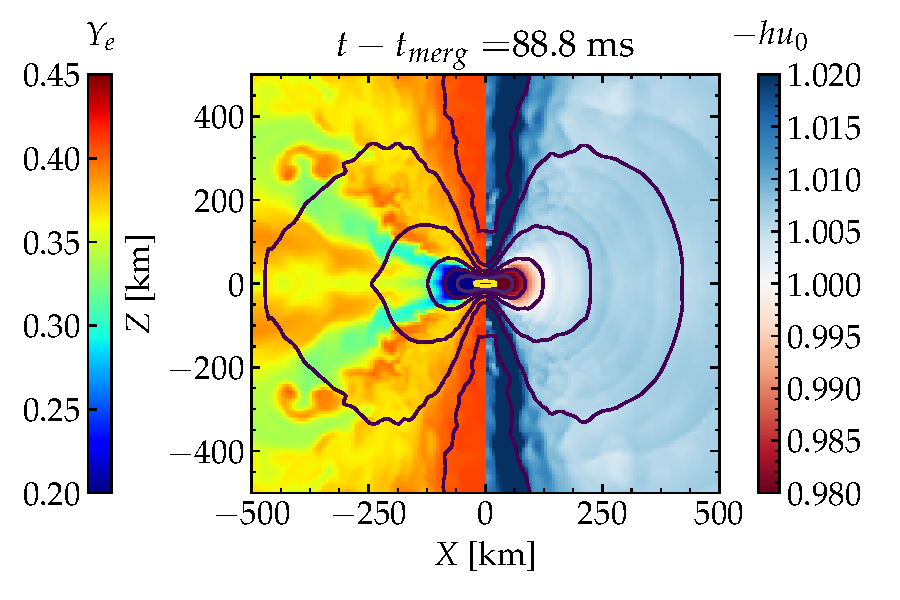
\includegraphics[width=0.49\textwidth]{slices/slice_xz_ye_hu_1.pdf}
    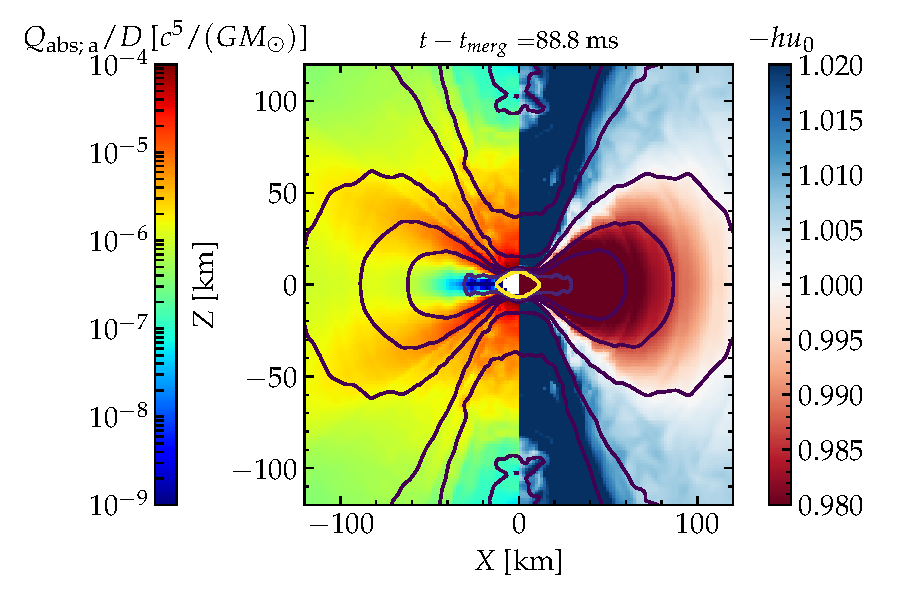
\includegraphics[width=0.49\textwidth]{slices/slice_xz_abs_energy_hu_3.pdf}
    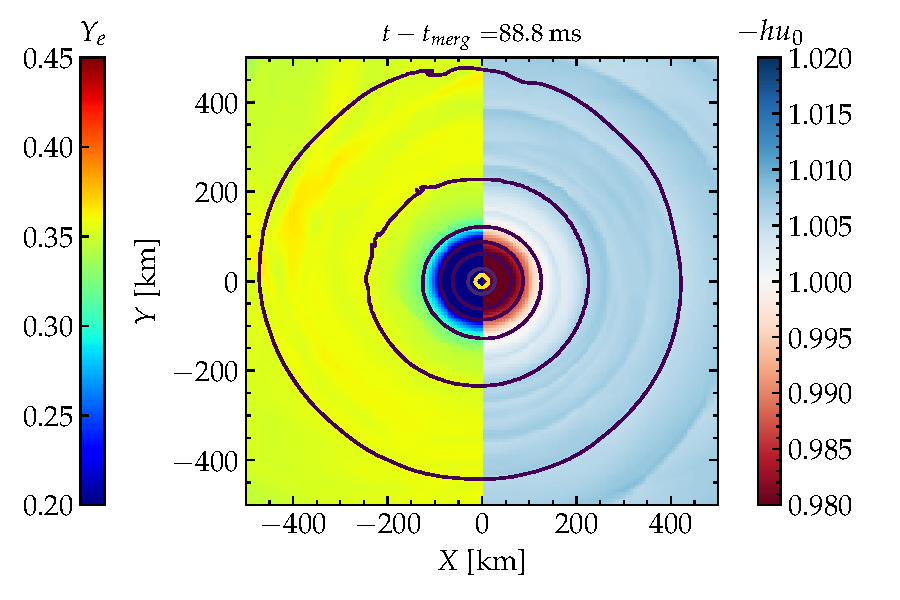
\includegraphics[width=0.49\textwidth]{slices/slice_xy_ye_hu_1.pdf}
    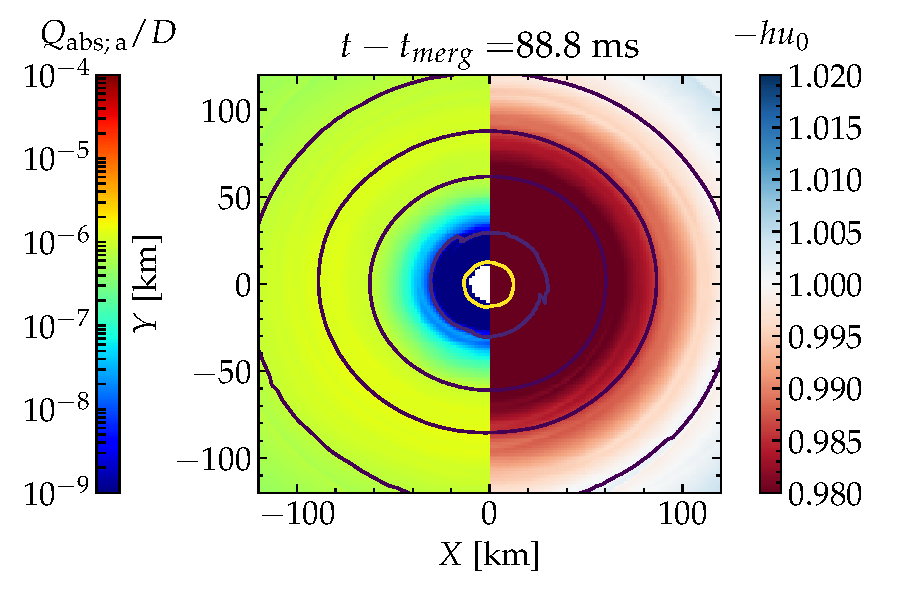
\includegraphics[width=0.49\textwidth]{slices/slice_xy_abs_energy_hu_3.pdf}
    \caption{Snapshot of the $(x,z)$ and $(x,y)$ slices of the BLh $q=1$ model at 
        ${\sim}89\,$ms after merger. Left panels: electron fraction and
        $-hu_0$. High $Y_e$ values indicate neutrino
        postprocessing and irradiation. The $-hu_0>1$ indicates the
        material that gains enough energy to become unbound at
        infinity. 
        %
        Right: $-hu_0$ and the absorption energy rate $Q_{\text{abs};\:\bar{\nu}_e}$ 
        of electron antineutrinos normalized to the fluid density $D$.
    }
    %
    \label{fig:slice:heating_hu}
\end{figure*}

In this section we investigate in detail the 
high electron fraction, polar component of the \acp{SWW}.
We propose that this outflow is mostly driven by the neutrino 
reabsorption, rather than by the dynamical mechanism responsible for the bulk of the 
\ac{SWW}.

The presence of the baryonic winds developing on the timescale of $\mathcal{O}(10)$~ms
and driven by the neutrino absorption above the remnant, where the neutrino flux is strong 
was reported before \citep[\eg][]{Perego:2014fma}. 

In this section we focus of the feducial model BLh $q=1.00$ (SR). 

In the left column of plots in Fig.~\ref{fig:slice:heating_hu} we compare 
the the Bernoulli parameter, 
$-hu_t$ (see Sec.\ref{sec:method:Bernoulli}), and the fluid electron 
fraction. 

In the right column of plots in Fig.~\ref{fig:slice:heating_hu} we compare 
the the Bernoulli parameter with the heating energy rate due to electron anti-neutrino absorption 
$Q_{\text{abs};\:\bar{\nu}_e}$ (see Sec.~\ref{method:M0:eq_for_Q}) divided by with 
$D=W\rho\sqrt{\gamma}$ (fluid's conserved rest-mass density)
We observe that the electron fraction in the polar region with angle 
from binary plane $\theta>60^{\circ}$ reaches $Y_e\sim0.35$ due to the absorption of 
electron-type neutrinos.
The strongest neutrino heating occurs in the vicinity of the remnant at densities 
$\rho\sim10^{11}$~\gcm, that roughly correspond to the region where neutrinos decouple,
the so-called neutrinosphere \citep{Endrizzi:2019trv}.

In Fig.~\ref{fig:slice:heating_hu} we compare the Bernoulli parameter, 
$-hu_t$ (see Sec.\ref{sec:method:Bernoulli}), that is always plotted 
on the right half of a panel, with the electron fraction (left 
column of plots and heating energy rate due to electron anti-neutrino absorption 
$Q_{\text{abs};\:\bar{\nu}_e}$ divided by with $D=W\rho\sqrt{\gamma}$ 
(fluid's conserved rest-mass density).
The observed correlation between the $E_\nu/D$ \red{???} and $-h u_t$ further suggests, 
that the outflow around the polar axis is driven by the neutrino absorption. 
Additionally, we found that if the neutrino absorption is not included into the 
simulation, \eg, using leakage only, the \nwind{} is absent. 
%% --- 
The collimated polar outflow can be further boosted and stabilized by the presence of the 
strong magnetic fields \citep{Bucciantini:2011kx,Ciolfi:2020hgg,Mosta:2020hlh}.
%% ---
Notably, there is not clear distinction between the \nwind{} and \ac{SWW}, especially 
at the intermediate latitudes ($\theta \sim 45^{\circ}$), where both mechanisms types of 
ejecta are present, and both, neutrino absorption and dyanmical effects driving the \ac{SWW} 
are contributing. 
%% --- 
In order to compute the mass flux of the \nwind{} an additional criterion is required. 
We consider two physically motivated criteria, the geometrical, flaggin the part of the \ac{SWW} 
and \nwind{} if it is polar, \ie, $\theta>60^{\circ}$, and the composition criterion, $Y_e > 0.35$.
%% --- 
We find that the \nwind{} is not a steady state outflow, contrary to the bulk of the \ac{SWW}.
After the initial strong rise, the mass flux rapidly decays in time, and for most models stops 
by the end of the simulations. This behaviour is independent of the criterion we use. 
We attribute it to the rise of the baryon loading above the remnant as the material gets lifted 
by thermal pressure from the disk.
The total mass of the \nwind{} is ${\sim}10^{-3}-10^{-4}M_{\odot}$. Its properties resemble those 
reported in e.g. \citet{Dessart:2008zd,Perego:2014fma,Fujibayashi:2020dvr}
Notably, in some of the works, the \nwind{} was found to require longer timescales to develop, 
achieving the quasi-steady state. 
This can be attributed to the strict criteria to isolate the \nwind{} and by the absence of the 
\ac{SWW} in other works. 
Additionally, our simulations might not be sufficiently long to achieve the donditions 
sufficient for the development of the quasi-steady state \nwind{}.
%% Additionally, as our models are at most $\sim100$~ms long, the conditions required for the steady 
%% state \nwind{} might not been achieved.



%% =======================================================
%%
%%                   Disc structure
%%
%% =======================================================


\section{Remnant disk structure}

\begin{figure}[t]
    \centering
    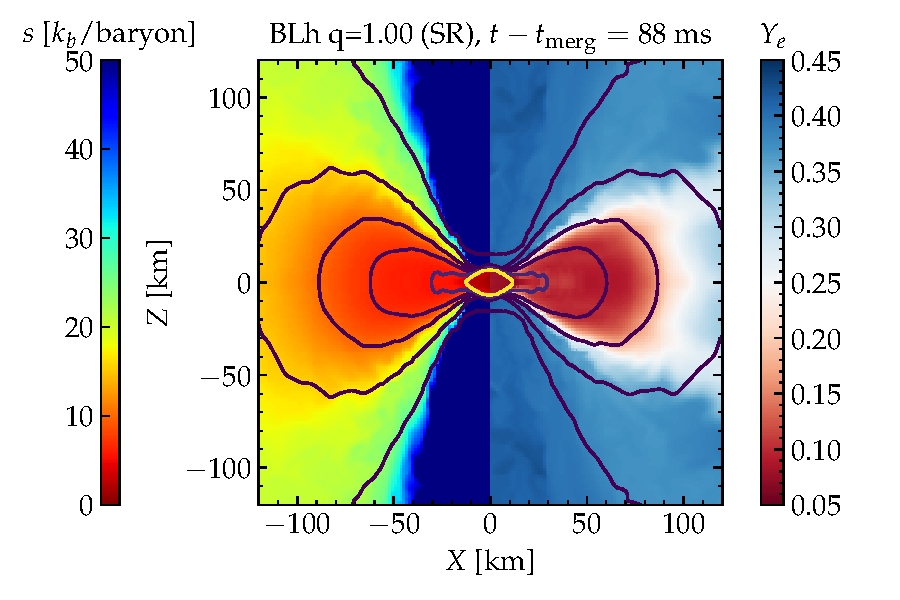
\includegraphics[width=0.49\textwidth]{disk/final_structure/slice_xz_entr_ye_blh_q1_rl3.pdf}
    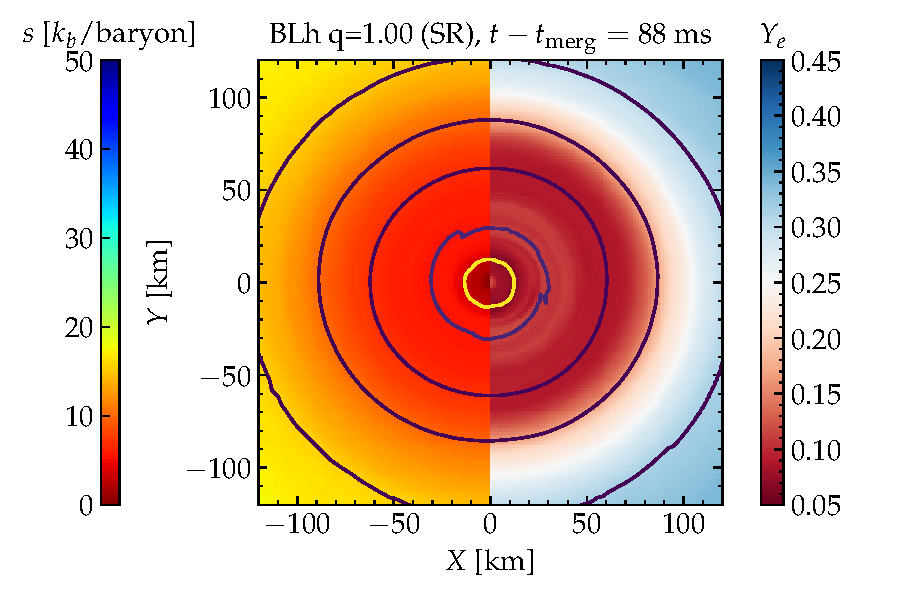
\includegraphics[width=0.49\textwidth]{disk/final_structure/slice_xy_entr_ye_blh_q1_rl3.pdf}
    \caption{Entropy and electron fraction on the $(x,z)$ (top) and
        $(x,y)$ planes (bottom) for the remnant of BL $q=1$ at the end
        of the simulation. Each plot is divided vertically, with entropy
        being color-coded on the left and electron fraction on the
        right. Solid contours stand for rest muss density. Counting from
        the center, the values are $[10^{13}, 10^{12}, 10^{11}, 10^{10},
        10^{9}]$ g cm$^{-3}$, with the inner most contour encompassing
        the remnant.
        (Adapted from \citet{Nedora:2020pak})
    }  
    \label{fig:snapshots_xy_ye_entr}
\end{figure}

\begin{figure*}[t]
    \centering 
    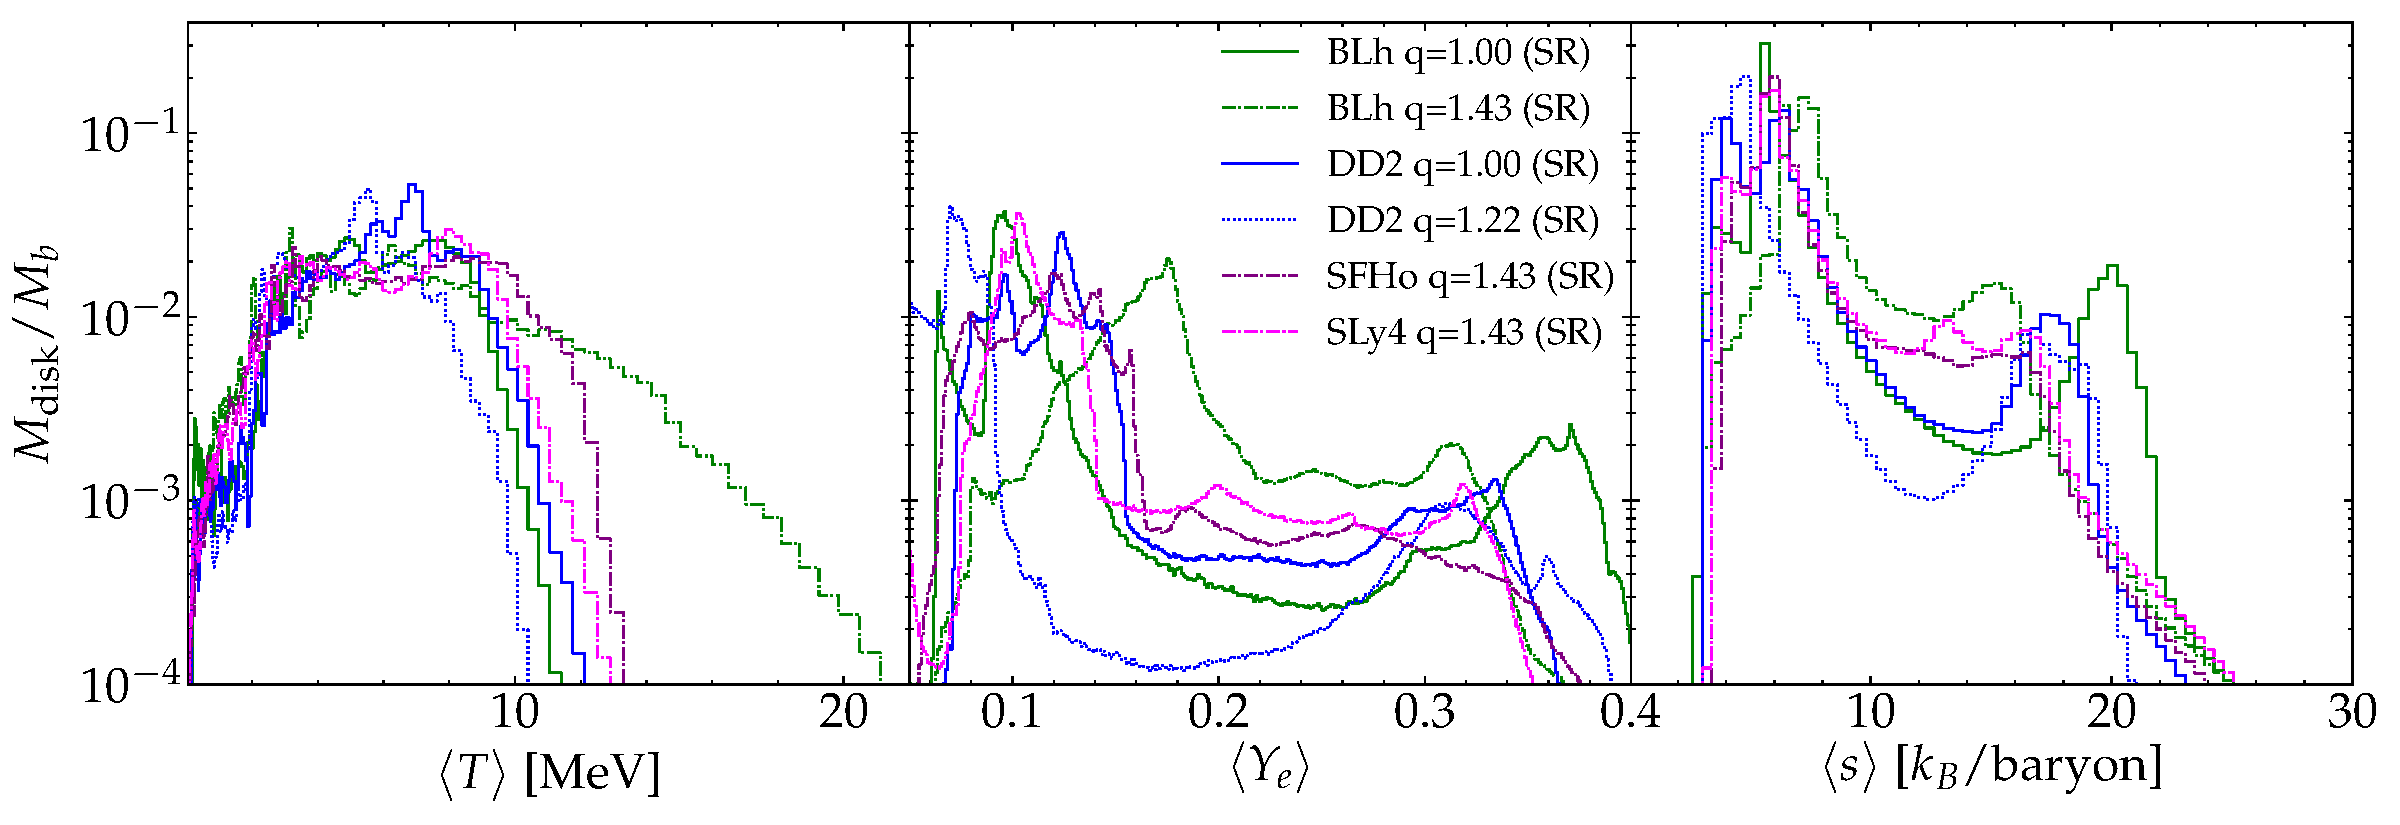
\includegraphics[width=0.95\textwidth]{disk/final_structure/disk_hist_shared.pdf}
    \caption{Composition of the disks at the end of the long-lived
        remnants simulations. The histograms refer to the temperature $T$
        (left),
        electron fraction $Y_e$
        (middle) and entropy $s$ (right).
        (Adapted from \citet{Nedora:2020pak})
    }
    \label{fig:final_disk_struct_hist_long}
\end{figure*}

In this section we discuss the final structure and properties of the disk, 
focusing on the models with long-lived \ac{MNS} remnants.
The properties are extracted at typical time $\sim60{-}100$~ms after merger.

We find that the generally the disk is optically thick.
The disk' RMS openning appears to be independent of the \ac{EOS} and \mr{} and
is $\langle\theta\rangle_{\text{rms}}\sim60^{\circ}$. 
The radial extend of the disk, however increases with the \ac{EOS} softness and 
binary \mr{}.
Similarly, the final disk mass is larger for the unequal mass binaries, 
ranging overall between ${\sim}0.1M_{\odot}$ and ${\sim}0.4M_{\odot}$
(see Tab.~\ref{tab:sim})..
Notably, for models with long-lived remnants the disk mass is larger,
that for the those with long-lived remnants. This can be attributed to the 
rapid accretion onto a \ac{BH} that removes $\sim50\%$ of the disk mass.
%% ---
We investigate the overall statistical properties of the disk mass for all our models
and those available in the literature in Sec.\ref{sec:results:Statistics:Mdisk}
\gray{
    The mean value of the disk mass in out models is 
    $\overline{M}_{\text{disk}}=(0.161 \pm 0.083)M_{\odot}$,
    where the standard deviation is also reported.
    %% ---
    Similarly to the dynamical ejecta we fit the disk masses with the 
    second order polynomial in $(q,\tilde{\Lambda})$.
    The coefficients of Eq.~\eqref{eq:fit:poly22}
    for this fit are given in Tab.~\ref{tab:fitpoly22coefs}.
    A more detailed study with various fitting formulas and extended
    datasets from the literature is reported in a companion paper.
}

Next, we consider the composition of the disk at the end of the simulation.
%% --- 
The mass-averaged temperature, electron fraction and entropy per baryon
are for several models are shown in Fig.~\ref{fig:final_disk_struct_hist_long}.
%% ---
We observe that the mass-weighted distribution of the entropy and electron 
fraction show a bimodal structure, which is more pronounced for the 
equal mass binaries. 
Regarding entropy, two peaks are present in the distribution:
a peak low entropy $s\sim5-10k_B/$baryon, that depends weakly of the 
\ac{EOS} and \mr{} and corresponds to the bulk, mildly shocked, material. 
The second peak is found at higher entropy, $s\sim15-22k_B/$baryon.
It corresponds fo the strongly shocked material and is more prominent 
in models with softer \ac{EOS}.
Notably, in the models with higher \mr{}, the second peak is located 
at lower $s$.
The mass-weighted distribution of the electron fraction 
displays a similar double-peak structure.
The low $Y_e$ peak that corresponds to the neutrino-shielded part of the 
disk is located around the $Y_e\sim0.1$.
The high $Y_e$ peak is located at $Y_e\sim0.3-0.4$ and corresponds to the outer parts of the disk, subjected to a strong neutrino irradiation.

In Fig.~\ref{fig:snapshots_xy_ye_entr} we show the electron fraction 
and entropy per baryon on the $xy$ and $xz$ slices of the equal 
mass model with BLh \ac{EOS}.
The plot shows, that the two peaks in the mass-weighted distribution 
of electron fraction and entropy correspond to different regions within the disk.

Overall, the most of the disk matter has temperature of $T\sim 1-10\,$MeV, with the innermost parts being hotter then the outer outermost. 
However, the disk temperature distribution appears to be largely independent of the \ac{EOS} and \mr{}

\red{Paragraph on the secular ejecta has been moved to 
    GW170817 application}

%% =======================================================
%%
%%                   Conclusion
%%
%% =======================================================




%% ========================================================================================

\section{Statistics of the \ac{DE} parameters and disk mass}

\red{CONTENT OF THE FIT PAPER}


\section{Application to \GW{}}


\begin{figure*}[t]
    \centering 
    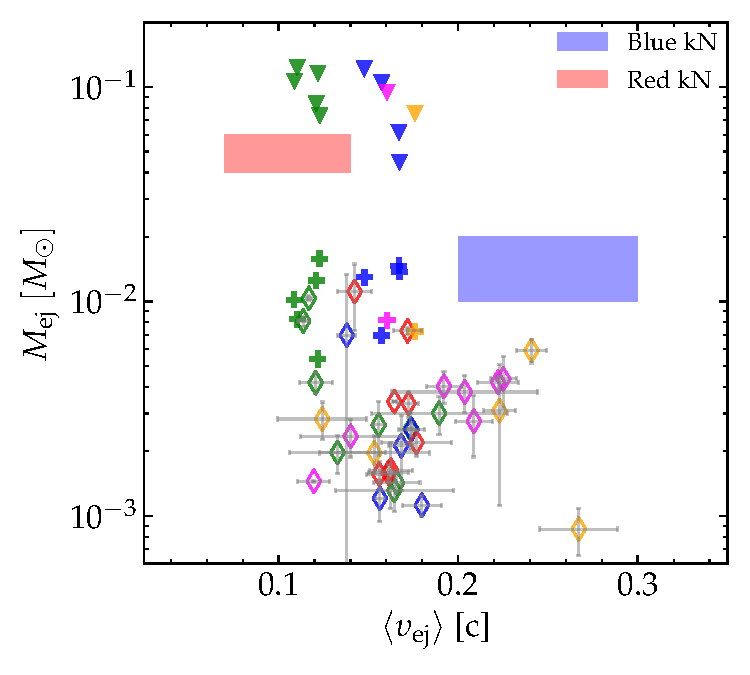
\includegraphics[width=0.48\textwidth]{ejecta_dyn/summary/ej_mej_vej_our2.pdf}
    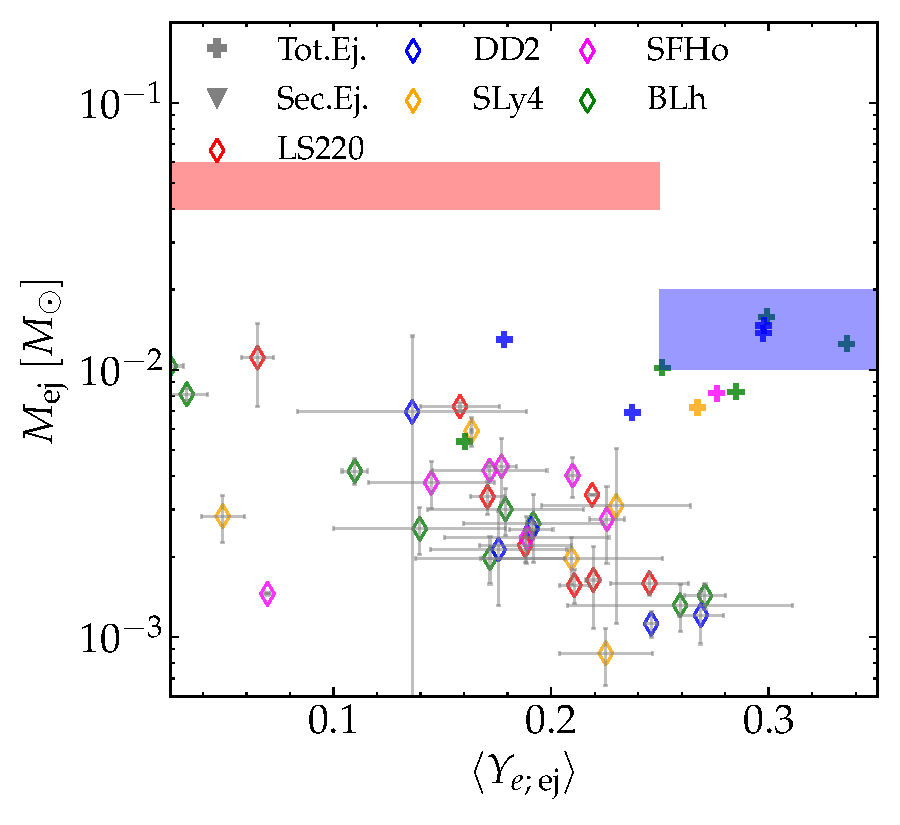
\includegraphics[width=0.48\textwidth]{ejecta_dyn/summary/ej_mej_yeej_our2.pdf}
    \caption{
        Summary of the ejecta properties of our models.
        %
        Diamonds mark the dynamical ejecta, crosses include the
        contribution of the \swind{} for the long-lived models, 
        triangles are an estimate of the total ejecta mass on a secular
        timescale, assuming $40\%$ of the disk mass is unbounded on
        secular timescales.         
        The ejecta mass is shown is terms of the mass-averaged velocity
        (left) and of the averaged electron fraction (right).
        %
        The filled blue and red patches are the expected values of
        ejecta mass and velocity for blue and red components of
        AT2017gfo compiled by \cite{Siegel:2019mlp}, based on
        \cite{Villar:2017wcc}. 
        Adopted from \citet{Nedora:2020pak}.
    }
    %
    \label{fig:ejecta:dyn:ds_sww}
\end{figure*}


%% from main paper, referencing the fitpaper Poly22 fits and SWW + DE
\red{THis can be augmented with Radio afterglow}

%% === FROM DYNAMICAL EJECTA SECTION of MAIN PAPER
Here we discuss the application of our results to \GW{}.


\subsection{Dynamical Ejecta}


%% ---
First, we asses the ejecta parameters that our fitting models, 
obtained in section \ref{sec:ejecta_disk_statisitcs} would provide for the \GW{}.
%% --- 
Considering the $90\%$ credible intervals estimated for $q$ and $\tilde{\Lambda}$ 
from LIGO-Virgo GW analysis
\citep{TheLIGOScientific:2017qsa,Abbott:2018wiz,De:2018uhw,Abbott:2018exr},
i.e.~$\tilde{\Lambda}=300_{-190}^{+500}$ and $q\in[1., 1.37]$. 
and using the errorbars formulas developed in \cite{Radice:2018pdn}, we find that
$\amd \in [0.72, 7.52] \times 10^{-3}\: M_{\odot}$
and
$\avd \in [0.16, 0.39]$c 
and 
$\ayd \in [0.11, 0.23]$.
Notably, these values do not agree with those inferred for \AT{} by the spherical, 
two-component kilonova models \citep{Villar:2017wcc}.
Analysis of a compiled set of kilonova fitting models provides a broad range of ejecta 
parameters \citep{Siegel:2019mlp}:
$M_{\text{ej}}^{\text{red}}\in(4, 6)\times10^{-2}M_{\odot}$ and
$\upsilon_{\text{ej}}^{\text{red}}\in(0.07, 0.14)$ for the red component, while
$M_{\text{ej}}^{\text{blue}}\in[1, 2]\times10^{-2}M_{\odot}$ and 
$\upsilon_{\text{ej}}^{\text{blue}}\in[0.2, 0.3]$ for the blue component.
%% ---
With respect to our results for \ac{DE}, however, 
none of the kilonova components can be well explained.
%% ---
In Fig.~\ref{fig:ejecta:dyn:ds_sww} we show the ejecta properties from
all our models (diamonds) and the parameters inferred from the
observations as red and blue boxes. 
%% --- 
With respect to the red component, we observe that \ac{DE} from our models 
have too high average velocities and not nearly enough mass.
This result suggests that an additional, low $Y_e$ ejecta component is required
in order to explain the \AT{} red component 
\citep{Perego:2017wtu,Kawaguchi:2018ptg,Nedora:2019jhl}.
%% --- 
A more thorough analysis of the \AT{} with better ejecta models and advanced
radiation transport kilonova simulations are not part of the present work 
and will be addressed in the future.


\subsection{Spiral-wave wind}


The \ac{SWW} could be a significant contributor to the \AT{}, assuming the remnant of 
\GW{} \ac{MNS} merger survived for $\mathcal{O}(100)$~ms.
%% ---- 
In Fig.~\ref{fig:ejecta:dyn:ds_sww} we report the total
(dynamical+\swind{}) ejecta mass and mass-averaged velocity for the
simulated long-lived BNS (crosses).
%% ---
Notably, the total ejecta mass of three of our models, 
BLh $q=1.18$, BLh $q=1.42$ and  DD2 is $q=1$ are in agreemnt with the epected values 
for the blue compoent of the \AT{} 
(obtained using the two-component fit \citep{Villar:2017wcc})

\red{
    [ LETTER STUFF COULD GO HERE ]
    a multi-component fitting model that explicitly accounts
    for the \swind{} can fit the early blue
    emission from AT2017gfo \citep{Nedora:2019jhl}
}

The high electron fraction of the \ac{SWW} however would result in a lanthanides-poor
composition of the outflow. Thus, the \ac{SWW} cannot explain the observed emission 
for the high opacity, lanthanides-rich material.
%% ---
Simulations with advanced physics of a \ac{MNS} mergers on a timescales $>100$~ms are 
required to asses the contribution from other outflow mechanisms, \red{that we will discuss below} 
\citep{Lee:2009uc,Fernandez:2015use,Siegel:2017nub,Fujibayashi:2017puw,Fernandez:2018kax,Radice:2018xqa}.


\subsection{Secular Ejecta}


On the timescale of seconds, much longer than the evolution of 
presented here simulations, the nuclear recombination can unbind 
a fraction of the disk mass. 
Analytical estimates and simulations with various approximations show that up tp ${\sim}40\%$ of the disk can be ejected via viscous processes with an typical velocity ${\lesssim}0.1\,$c
\citep{Lee:2009uc,Fernandez:2015use,Wu:2016pnw,Siegel:2017nub,Fujibayashi:2017puw,Fernandez:2018kax,Radice:2018xqa,Fujibayashi:2020dvr}.

Adapting the fix fraction of the $40\%$ of the disk mass, we estimate 
that about  ${\sim}0.05\, M_{\odot}$ would be ejected in a form of 
secular winds. We include this estimate for every simulation
with the long-lived \ac{MNS} remnant in Fig.~\ref{fig:ejecta:dyn:ds_sww} (lower triangles).
The estimated mass is sufficient to explain
the red component of AT2017gfo, as inferred from the two-components kN
models of \cite{Villar:2017wcc}. 







%% ---------------------
Sources with time delay are preferred by studies of very metal poor stars that indluded the time delay for r-process elements
to diffuse through ISM, \citep{Tarumi:2021xvw}. 
A winds from proto-nuetron are also contributors to the $r$-process budget \cite{Vincenzo:2021rvw}

\red{The remnant is losing anular momentum while disk gains on shortly after merger is due to gravitational torque \cite{Shibata:2019wef}}

\chapter{Modern methods in numerical relativity}\label{ch:nr_methods}

In this thesis we perform numerical simulations of \ac{BNS} mergers. 
In the simulations the \ac{EFE} descibing the spacetime dynamics, are formulated in a 
way more suitable for numerical applications. We discuss this formulations in 
Sec.~\ref{sec:method:nr:gr}, where we summarize the equations for \ac{NR}.
The basis of \ac{EFE} and \ac{GR} is not covered here for the sake of brevity. For that we 
refer to \citet{Arnowitt:1962hi,Landau:1982dva,Wald:1984,Misner:1973,Baumgarte:2002jm}.


\section{Numerical implementation of General Relativity}\label{sec:theory:nr}

%%%% === Additional Intro
%The \ac{EFE} is the foundation of modern cosmology, the physics of \acp{NS} and \acp{BH},
%the emission of gravitational radiation, and numerous other cosmic phenomena, 
%where strong gravity effects are present. The Einstein theory of \ac{GR} has 
%passed numerous tests in the weak-field regime \citep{Asmodelle:2017sxn} and in a 
%strong field regime when the gravitaional radiation from the merger of two \acp{BH} was 
%detected for the first time \citep{Abbott:2016blz}.

\ac{EFE} in a covariant form, neglecting the cosmological constant, read
%
\begin{equation}
    G_{\mu\nu} = R_{\mu\nu} - \frac{1}{2} R g_{\mu\nu} = 8\pi T_{\mu\nu}
\end{equation}
%
(As an exercise we provide a short derivation of the 
\ac{EFE} from the variation of Hilbert action in Appendix~\ref{app:efe})
%
where $R_{\mu\nu}$ is the Ricci curvature tensor with its trace 
$R^{\mu}_{\nu} = R$, $g_{\mu\nu}$ is the metric tensor and 
$T_{\mu\nu}$ is the stress-energy tensor.
%
However, for numerical applications it is desirable to represent the as an \ac{IVP},
where the once the initial data is specified at time zero, the evolution is computed.
An approach that is widely used, is the \textit{$3+1$ decomposition}, where the $4$D 
manifold is represented as foliation of $3$D spacelike hypersurfaces 
\citep{Alcubierre:2008,Baumgarte:2010,Gourgoulhon:2007ue,Rezzolla:2013}.


\subsection{3+1-Decomposition}

\begin{figure}[t]
    \centering 
    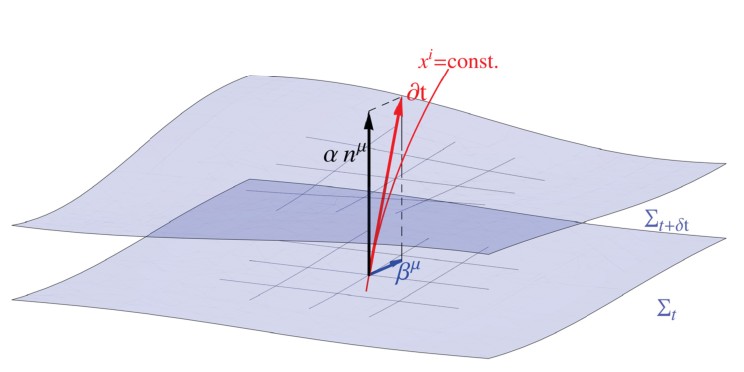
\includegraphics[width=0.49\textwidth]{tim_3p1_plot.pdf}
    \caption{
        Visual representation of the $4$D manifold $\mathcal{M}$ by $3$D hypersurfaces 
        $\Sigma_t$. The lapse function $\alpha$ and shift vector $\beta^{\mu}$ describe the 
        coordinate change between hypersurfaces.
        Adopted from \citet{Dietrich:2016phd}.
    }
    \label{fig:theory:3p1}
\end{figure}

Eq.~\eqref{eq:theory:EFE} represent a set of $10$ non-linear \acp{PDE}. 
These equations can be defined on a whole metric $\mathcal{M}$ or a domain $\Omega\subset\mathcal{M}$,
where in the latter case, the boundary conditions on $\partial\Omega$ are required. 
%
The initial data is defined on a null hyersurface $\Sigma\subset\mathcal{M}$, 
from which the evolution of space-time begins. 
This requires the spacetime to be strongly hyperbolic, 
meaning that the foliation $\mathcal{M}=\Sigma\times\mathbb{R}$ is allowed. 
This foliation can be understood as splitting the spacetime into a set of 
spacelike hypersurfaces $\Sigma_t$ as depicted in Fig.~\ref{fig:theory:3p1}. 


%%%% ==== Basicas of Foliations, Lapse, Shift, Norm
Let the $t$ be the global smooth functions such that, 
$\Sigma_{\tau} = \{x^{\alpha}\in\mathcal{M}: t(x^{\alpha})=\tau\}$ 
and let $\vec{t}$ be a vector such that $\langle\nabla t, \vec{t}\rangle = 1$,
where $\nabla$ denotes the covariant derivative.
%
This $t$ can be seen as a "function that advances time" and $\vec{t}$ as a "flow of time" vector field. 
Continuing the analogy, the rate at which a given tensor quantity changes 
between hypersurfaces $\Sigma_t$ is given by the Lie derivative
\footnote{
    Lie derivative evaluates the change of a tensor field, along the flow 
    defined by another vector field. This change is coordinate invariant 
    and therefore the Lie derivative is defined on any differentiable manifold.
} of the $\boldsymbol{q}$ along the vector $\vec{t}$.
%
Consider now two hypersurfaces $\Sigma_t$ and $\Sigma_{t+dt}$ (Fig.~\ref{fig:method:3p1}). 
A transition from one to another can be decomposed into the part tangent to the hypersurface 
$\Sigma_{t+dt}$ and expressed in a form of a vector $\vec{\beta}$, and a part normal to the hypersurface 
$\Sigma_t$ and expressed as a $\alpha \vec{n}$, where $\vec{n}$ is a unit vector, 
normal to the $\Sigma_t$ in the direction to $\Sigma_{t+dt}$, \ie, $n_{\mu} = -\alpha \nabla_{\mu}t$.
%
Then, the vector $\vec{t}$ can be written as 
%
\begin{equation*}
\vec{t} = \alpha\vec{n}+\vec{\beta}.
\end{equation*}
%
%%%% ==== More on the metric and decompositions
%The spacetime metric $\boldsymbol{g}$ can be decomposed into a spatial, 
%Riemannian metric $\boldsymbol{\gamma}$, as 
%$\boldsymbol{\gamma} = \boldsymbol{g} + \underline{n} \otimes \underline{n} $, 
%where $\underline{n}$ is the $1$-form associated to the vector $\vec{n}$, 
%and $\otimes$ denotes the product measure.
%%
%The Levi-Civita connection can be computed by projecting the 
%$\nabla$ on the space, tangent to the hypersurface $\Sigma_t$.
%
%Next, we need to discuss two important entities, 
%the three-metric, and the extrinsic curvature.
%%
%There are exist coordinates that are adapted to the $3+1$ foliation, namely $\{t, x^i\}$ 
%with $\vec{\partial}_i \cdot \vec{n} = 0$. 
%In these coordinates the $\nabla t = dt$ and $\vec{t} = \vec{\partial}_t$, 
%where hereafter $\nabla$ denotes a covariant derivative.
%
%The connection between $\boldsymbol{g}$ and $\boldsymbol{\gamma}$ is $g_{\mu\nu}=\vec{\partial}_{\mu}\cdot\vec{\partial}_{\nu} $ 
%and can be expressed in terms of $\alpha$ and $\vec{\beta}$.
%\begin{align}
%\text{spatial components: } g_{ik}&=\vec{\partial}_{i}\cdot\vec{\partial}_{j} =\gamma_{ik}, \\
%\text{time component: } g_{tt} &= \vec{\partial}_{t}\cdot\vec{\partial}_{t} = \vec{t}\cdot\vec{t} = - (\alpha^2-\vec{\beta}\cdot\vec{\beta}), \\
%\text{mixed components: } g_{ti} &= \vec{\partial}_{t}\cdot\vec{\partial}_{i} = \vec{t}\cdot\vec{\partial}_i = (\alpha\vec{n}+\vec{\beta})\cdot\vec{\partial}_i=\beta_i,
%\end{align}
%we we made use of $\vec{\beta}$ being the spatial vector, \textit{i.e} $\vec{\beta}\cdot\vec{\beta}=\gamma_{ik}\beta^i\beta^k$.
% 
%The line-element can be thus written as
%\begin{equation}
%ds^2 = -(\alpha^2-\beta_i\beta^i)dt^2 +2\beta_i dx^i dt + \gamma_{ik} dx^i dx^k.
%\end{equation}

%%%% === Extrinsic curvature
Next, consider the extrinsic curvature of a $D-1$-surface $\Sigma_t\subset\mathcal{M}$
at a point $\mathcal{P}\in\Sigma_t$ as mapping $\boldsymbol{K}$ such that $\boldsymbol{K}(\boldsymbol{\upsilon})=-\nabla_{\boldsymbol{\upsilon}}\boldsymbol{n}$. 
Note, that the $\boldsymbol{K}$ thus does not depend on $\alpha$ and $\vec{\beta}$, 
it is a purely spatial tensor. The components of the extrinsic curvature are
%
\begin{equation}
    K_{\mu\nu} = -{\gamma^{\alpha}}_{\mu}\nabla_{\boldsymbol{u}}^{\alpha} n_{\nu} = -\frac{1}{2}\mathcal{L}_{\vec{n}}\gamma_{\mu\nu},
    \label{eq:theory:extrcurvdef}
\end{equation}
%
where $\mathcal{L}_{\vec{n}}$ is the Lie derivative along the vector field $\vec{n}$. \\
From the (\ref{eq:theory:extrcurvdef}) 
%
The extrinsic curvature can be interpreted as a "speed of the $\vec{n}$ during the parallel 
transport along the hypersurface $\Sigma_t$".


\subsection{Gauge conditions}

%% === For the lapse function
The gauge condition describes the specific foliation of the spacetime, the choice of the 
lapse function and shift vector. 
%
Numerical simulations depend strongly on the its choice. An incorrect choice might result in development of 
gauge\footnote{Gauge shocks are coordinate singularities for which the lapse becomes discontinuous
    caused by the crossing of characteristic lines \citep{Alcubierre:2002kk}
} and slice stretching \citep{Reimann, 2004; Reimann, 2005}. Additionally, a well-posedness of the 
\ac{PDE} must be ensured for stable numerical evolution.

One of the widely used slicing conditions is the Bona-Mass{\'o} slicing \citep{Bona:1994dr}, 

\begin{equation}
    \partial_t - \beta^i\partial_i)\alpha = -\alpha^2 f(\alpha)K,
    \label{eq:theory:slicing_a}
\end{equation}

where $f(\alpha)$ is a positive function, and $K$ is the trace of extrinsic curvature.
When if $f=1$ one gets the geodesic slicing, and if $f\rightarrow\infty$, it resembles the 
maximal slicing \citep{Baumgarte:2002jm}.
In this thesis we employ the so-called ``1+log'' slicing, when $f(\alpha) = = 2/\alpha$.
The name stems from the fact that if $\beta^i = 0$, the integration of Eq.~\eqref{eq:theory:slicing_a} 
yields $\alpha = 1 + \log \gamma$.
The condition allows for good singularity avoidance at zeroth order \cite{Alcubierre:2002kk} and 
does not lead to gauge shocks, and numerically not very expensive, as it is formulated in form 
of hyperbolic equations.

%% === for the shift vecotor
For the spatial gauge condition, the choice of $\beta^i,$ we consider the Gamma-driver 
\cite{Alcubierre:2002kk,vanMeter:2006vi}, that in integrated from reads 

\begin{equation}
    (\partial_t - \beta^j\partial_j)\beta^i = \mu_S\overline{\Gamma}^i - \eta\beta^i
    \label{eq:theory:slicing_b}
\end{equation}

where $\overline{\Gamma}^i$ is the conformal connector (discussed later), $\eta$ is the 
dampening parameter, and $\mu_s$ is the gauge parameter.
The requirements for spatial gauge are similar as in the case of the one for $\alpha$, 
namely, hyperbolicity and minimization of numerical distortions for more stable evolution. 
This gauge condition tries to decrease the coordinate stretching that occur in the 
vicinity of a singularity. It was shown to be effective in numerical applications, 
in particular for a single moving black hole. However it has a zero-speed mode, 
that can amplify the numerical errors and destabilize the system \citep{vanMeter:2006vi}.
%
The combination of Eq.~\eqref{eq:theory:slicing_a} and Eq.~\eqref{eq:theory:slicing_b}
is usually referred to as \textit{moving puncture} gauge. 
%
\gray{Together with the Z4c 
    formualtion of \ac{EFE} (discussed below) it forms a strongly hyperbolic system of equations}


\subsection{$3+1$-from of Einstein's Field Equations}

Here we consider the dynamics of the gravitational field in the $3+1$ formalism.

\subsubsection{ADM-Equations}

\red{somewhere here put that angular momentum is not defined in GR}

The goal is to split \ac{EFE} Eq.~\eqref{eq:theory:EFE} into a set of constraint and evolutionary 
equations. Consider the \ac{RHS} of Eq.~\eqref{eq:theory:EFE}, the energy-momentum tensor, 
$T_{\mu\nu}$ in $3+1$ form. For that we employ the spatial projection operator 
$P^{\mu}_{\nu} = \delta_{\nu}^{\mu} + n^{\mu}n_{\nu}$, and obtain that 

\begin{subequations}
    \begin{align}
    S_{\mu\nu} &= P^{\sigma}_{\mu} P^{\rho}_{\nu} T_{\sigma\rho} \label{eq:theory:s_munu}\\
    S_{\mu} &= -P^{\sigma}_{\mu} n^{\rho} T_{\sigma\rho} \label{eq:theory:smu}
    \end{align}
\end{subequations}

where $S_{\mu\nu}$ is the spatial part of $T_{\mu\nu}$, $S_{\mu}$ is the momentum density, 
$S=S^{\mu}S_{\mu}$ is the trace, $E=n^{\mu}n^{\nu}T_{\mu\nu}$ is the energy density measured by 
the Eulerian observer with the four-velocity $n^{\nu}$.

%% === Constraint Equations
Next we use the fact that the Gauss (Gauss-Codazzi) equation relates the $3$D Riemann tensor
$^3{R_{\alpha\beta\gamma}}^{\delta}$ to the $4D$ one and the $\boldsymbol{K}$, and that the 
Codazzi (Codazzi-Mainardi) equations relate the $4D$ Ricci tensor to the extrinsic curvature,
to perform a split for the Reimann tensor as follows:

\begin{subequations}
    \begin{align}
        P_{\alpha}^{\delta}P_{\beta}^{\kappa}P_{\mu}^{\lambda}P_{\nu}^{\sigma} {^{(4)}R}_{\delta\kappa\lambda\sigma} 
        &= {^{(3)}R}_{\alpha\beta\mu\nu} + K_{\alpha\mu}K_{\beta\nu} - K_{\alpha\nu}K_{\beta\mu} \label{eq:theory:gc}\\
        %
        P_{\alpha}^{\delta}P_{\beta}^{\kappa}P_{\mu}^{\lambda}n^{\sigma} {^{(4)}R}_{\delta\kappa\lambda\sigma} 
        &= D_{\beta}K_{\alpha\mu} - D_{\alpha}K_{\beta\mu}, \label{eq:theory:gm}
    \end{align}
\end{subequations}

where $P^{\alpha\beta} = \gamma^{\beta\omega}p_{\omega}^{\alpha} = \gamma^{\alpha\beta}$, 
$^{(3)}R_{\alpha\beta\mu\nu}$ is the 3D Riemann tensor and $D_{\mu}$ is the 3D covariant derivative after 
the projection of $\nabla_{\mu}$ onto the space orthogonal to $n^{\alpha}$.
%
From the Eq.~\eqref{eq:theory:gc}, combining the contracted Gauss relation and \ac{EFE} Eq.~\eqref{eq:theory:EFE}, one obtains 

\begin{equation}
    \gamma^{\alpha\gamma}\gamma^{\beta\delta} {^{(4)}R}_{\alpha\beta\gamma\delta} = {^{(3)}R} + K^2 - K_{\alpha\beta}K^{\alpha\beta} = 2n^{\alpha}n^{\beta}G_{\alpha\beta} = 16\pi E.
\end{equation}

From the contraction of Eq.~\eqref{eq:theory:gm}, results in

\begin{equation}
    \gamma^{\alpha\mu}n^{\nu}{^{(4)}R_{\mu\nu}} = D^{\alpha}K - D_{\mu}K^{\alpha\mu} = \gamma^{\alpha\mu}n^{\nu}G_{\mu\nu} = 8\pi S^{\alpha}.
\end{equation}

The obtained two sets of equations 

\begin{align}
    {^{(3)}R} + K^2 - K_{\alpha\beta} K^{\alpha\beta} &= 16\pi E, \label{eq:theory:ham_const}\\
    D_j K^{ij} - D^i K &= 8\pi S^i, \label{eq:theory:mom_const}
\end{align}

are called \textit{Hamiltonian} and \textit{Momentum Constraints}, respectively.
%
The obtained constraint equations represent a set of elliptic equations 
that must be satisfied on every hypersurface $\Sigma_i$ of the foliation. 
%
It is however, possible to show that \ac{EFE} preserve the constraints, 
meaning that if they are satisfied at the initial slice $\Sigma_0$ 
they will be satisfied at any time in the future.

%% === Evolution Eqs
Next we consider the evolution equations

Consider the induced metric 

\begin{equation}
    \partial_t\gamma_{ij} = -2\alpha K_{ij} + D_{i}\beta_j + D_j \beta_i,
    \label{eq:theory:evol_metric}
\end{equation}

and expand the definition of the extrinsic curvature as 

\begin{equation}
    \begin{aligned}
    K_{\alpha\beta} = \frac{1}{2}(K_{\alpha\beta} + K_{\beta\alpha}) = -\frac{1}{2}(n^{\mu}n_{\beta}\nabla_{\mu}n_{\alpha} + \nabla_{\beta}n_{\alpha}+n^{\mu}n_{\alpha}\nabla_{\mu}n_{\beta}+\nabla_{\alpha}n_{\beta}) = \\
    -\frac{1}{2}(n^{\mu}\nabla_{\mu}(n_{\alpha}n_{\beta}) +g_{\alpha\mu}\nabla_{\beta}n^{\mu} + g_{\beta\mu}\nabla_{\alpha}n^{\mu}) = -\frac{1}{2}(n^{\mu}\nabla_{\mu}\gamma_{\alpha\beta} + \gamma_{\alpha\mu} \nabla_{\beta} n^{\mu} + \gamma_{\beta\mu}\nabla_{\alpha}n^{\mu}) = \\
    -\frac{1}{2}\mathcal{L}_{n}\gamma_{\alpha\beta} = -\frac{1}{2\alpha}(\mathcal{L}_t - \mathcal{L}_{\beta})\gamma_{\alpha\beta} = -\frac{1}{2\alpha}(\partial_t\gamma_{\alpha\beta} - D_{\alpha}\beta_{\beta} - D_{\beta}\beta_{\alpha})
    \end{aligned}
\end{equation}

Then, the evolution equation for the extrinsic curvature reads 

\begin{equation}
    \begin{aligned}
    \partial_t K_{ij} = -D_i D_j \alpha + \beta^k \partial_k K_{ij} + K_{ik}\partial_j \beta^k + K_{kj}\partial_i \beta^k + \\
    \alpha({^{(3)}R_{ij}} + KK_{ij} - 2K_{ik}{K^k}_j) + 4\pi \alpha (\gamma_{ij}(S-E) - 2S_{ij})
    \end{aligned}
    \label{eq:theory:evol_eq}
\end{equation}

This equation is obtained from the following considerations. 
First the Riemann tensor was contracted twice with the normal vector, applying the 
Eq.~\eqref{eq:theory:gc}, as 

\begin{subequations}
    \begin{align}
    P_{\alpha}^{\mu}P_{\beta}^{\nu}n^{\rho}n^{\sigma}{^{(4)}R_{\mu\rho\nu\sigma}} = \mathcal{L}_{n} K_{\alpha\beta} + \frac{1}{\alpha} D_{\alpha}D_{\beta}\alpha + {K^{\lambda}}_{\beta}K_{\alpha\lambda} \label{eq:theory:for_ev1}\\
    %
    P_{\alpha}^{\mu}P_{\beta}^{\nu}(n^{\rho}n^{\lambda} {^{(4)}R_{\mu\rho\nu\lambda}} + {^{(4)}R_{\mu\nu}}) = 
    {^{(3)}R_{\alpha\beta}} + KK_{\alpha\beta} - {K^{\lambda}}_{\beta}K_{\alpha\lambda}. \label{eq:theory:for_ev2}
    \end{align}
\end{subequations}

Next, inserting Eq.~\eqref{eq:theory:for_ev1} in Eq.~\eqref{eq:theory:for_ev2} yields

\begin{equation}
    \mathcal{L}_n K_{\alpha\beta} = -\frac{1}{\alpha} D_{\alpha} D_{\beta} \alpha - P^{\mu}_{\alpha}P_{\beta}^{\nu} {^{(4)}R_{\mu\nu}} + {^{(3)}R_{\alpha\beta}} + KK_{\alpha\beta} - 2{K^{\lambda}}_{\beta}K_{\alpha\lambda}
\end{equation}

The latter can be reformulated to match the colution equation Eq.~\eqref{eq:theory:evol_eq}.
%
Equations \eqref{eq:theory:ham_const},\eqref{eq:theory:mom_const}, \eqref{eq:theory:evol_metric} and 
\eqref{eq:theory:evol_eq} comprise the  \ac{IVP} for \ac{EFE} and are known as \ac{ADM} 
system of equations \cite{Arnowitt:1962hi}.
(We present a derivation with mores steps in Appendix~\ref{app:adm}).
%
They determine how to set the initial 
data on the hypersurface $\Sigma_0$, via prescribing the three-metric and extrinsic curvature. 


%% Strongly hyperbolic formulations of EFE
It has been shown, that the \ac{ADM} system of equations in its original form 
%% Eq.~\eqref{eq:theory:adm} 
is only weekly hyperbolic \citep{Baumgarte:2002jm}. Specifically, it was shown that the numerical 
errors tend to couple with zero-velocity modes \citep{Alcubierre:1999rt}. 
In an attempt to tackle this problem, other formulations of the \ac{EFE} as \ac{IVP} were proposed. 
%
%%%% === OTHER FOMULATIONS OF EFE 
%In particular, the generalized-harmonic formulation \citep{Friedrich:1986,Garfinkle:2001ni,Pretorius:2004jg,Lindblom:2005qh}. 
%It has an advantage of allowing for dampening of the constraint violation \citep{Gundlach:2005eh} and
%constraint-preserving boundary conditions \citep{Kreiss:2006mi,Rinne:2005df,Ruiz:2007hg}.
%%
%The BSSNOK formulation, was derived by Baumgarte, Shapiro, Shibata, Nakamura, Oohara and Kojima \citep{Nakamura1987,Shibata:1995we,Baumgarte:1998te}. It had an advantage of allowing to choose 
%conformal variables and was not bound to a given gauge condition 
%(thus a gauge beneficial for \acp{BH} evolution, \ie, moving puncture gauge can be used). 
%However, it had zero-speed characteristic variables that could lead to the large 
%Hamiltonian constraint violation in \ac{NR} applications.
%%
%And the Z4 formulation \citep{Bona:2003fj,Bernuzzi:2009ex,Ruiz:2010qj,Weyhausen:2011cg,Alic:2011gg}.
%%% 
%%The Z4c formulation of \ac{EFE} was developed in a series of works by \citet{Bernuzzi:2009ex,Ruiz:2010qj,Weyhausen:2011cg,Cao:2011fu,Hilditch:2012fp} and 
%%summarized in \citet{Hilditch:2012fp}. 
%The idea behind the Z4 formulation is to derive a set of evolution equations that is free from the 
%zero-speed modes of the original \ac{ADM} and thus -- strongly-hyperbolic. 
%This is achieved by not explicitly enforcing the constraints and treating the deviation 
%from them as an dependent variable $Z_{\mu}$. 
%The $Z_{\mu}$ is also called the Z4 four-vector.


\subsubsection{Z4c-evolution system}

The Z4c formulation of \ac{EFE} was developed in a series of works by \citet{Bernuzzi:2009ex,Ruiz:2010qj,Weyhausen:2011cg,Cao:2011fu,Hilditch:2012fp} and 
summarized in \citet{Hilditch:2012fp}. 
%
The idea behind the Z4 formulation is to derive a set of evolution equations that is free from the 
zero-speed modes of the original \ac{ADM} and thus -- strongly-hyperbolic,
and also inherit the constraint violation dampening properties of the original Z4 formulation.

The \ac{EFE} equations read 

\begin{equation}
    R_{\alpha\beta} + \nabla_{\alpha}Z_{\beta} + \nabla_{\beta}Z_{\alpha} = 8\pi \Big( T_{\alpha\beta} - \frac{1}{2}g_{\alpha\beta}T \Big) + \kappa_1 (t_{\alpha} Z_{\beta} + t_{\beta}Z_{\alpha} - (1+\kappa_2)g_{\alpha\beta})t_{\gamma}Z^{\gamma},
    \label{eq:theory:z4c_efe}
\end{equation}

where $Z_{\alpha}$ is a four-vector consisting of constraints, $t_{\alpha}$ is a timelike vector and 
$\kappa_1$ and $\kappa_2$ are the dampening parameters.
Eq.~\eqref{eq:theory:z4c_efe} is equivalent to Eq.~\eqref{eq:theory:EFE} when constraints are satisfied.
%
In $3+1$ from the equations read 
\begin{subequations}
\begin{align}
    \widetilde{\gamma}_{ij} = \chi\gamma_{ij} \label{eq:theory:z4c_1}\\
    \widetilde{A}_{ij} = \chi(K_{ij}-\frac{1}{3}\gamma_{ij}K)\label{eq:theory:z4c_2} \\
    \hat{K} = \gamma^{ij}K_{ij} - 2\Theta,\label{eq:theory:z4c_3}
\end{align}
\end{subequations}

where $\Theta=-n_{\alpha}Z^{\alpha}$.

Inserting Eq.~\eqref{eq:theory:z4c_1},\eqref{eq:theory:z4c_2} and \eqref{eq:theory:z4c_3} into
Eq.\eqref{eq:theory:z4c_efe} yields the 
The equations of motion for the Z4c formulation:
%
\begin{equation}
    \begin{aligned}
    \partial_t\chi =& \frac{2}{3}\chi \Big[ \alpha (\hat{K} + 2\Theta) - D_i\beta^i \Big], \\
    \partial_t\bar{\gamma}_{ij} =& -2\alpha\widetilde{A}_{ij} + \beta^k\partial_k\widetilde{\gamma}_{ij} + 
    2\widetilde{\gamma}_{k(i}\partial_{j)}\beta^k - \frac{2}{3}\widetilde{\gamma}_{ij}\partial_k\beta^k, \\
    %% for the metric components,
    \partial_t\hat{K} =& -D^{i}D_{i}\alpha + \alpha \Big[ \widetilde{A}_{ij}\widetilde{A}^{ij} + \frac{1}{3}(\hat{K} + 2\Theta)^2 \Big]  \\
    & + 4\pi \alpha [S + \rho] + \alpha \kappa_1 (1 - \kappa_2)\Theta + \beta^i\partial_i\hat{K},  \\
    \partial_t\widetilde{A}_{ij} =& \chi [ -D_i D_j \alpha + \alpha(R_{ij} - 8\pi S_{ij}) ]^{\text{tf}} + 
    \alpha \Big[ (\hat{K} + 2\Theta)\widetilde{A}_{ij} - 2 {\widetilde{A}^k}_i\widetilde{A}_{kj} \Big] \\
    & + \beta^k\partial_k\widetilde{A}_{ij} + 2\widetilde{A}_{k(i}\partial_{j)}\beta^k - \frac{2}{3}\widetilde{A}_{ij}\partial_{k}\beta^{k},  \\
    %% for extrinsic curvature
    \partial_t\widetilde{\Gamma}^i =& -2\widetilde{A}^{ij}\partial_j\alpha + 2\alpha\Big[ {\widetilde{\Gamma}^i}_{jk}\widetilde{A}^{jk} - 
    \frac{3}{2}\widetilde{A}^{ij}\partial_j\ln(\chi) - \frac{1}{3}\widetilde{\gamma}^{ij}\partial_j(2\hat{K}+\Theta) - 8\pi\widetilde{\gamma}^{ij}S_j \Big] \\
    & + \widetilde{\gamma}^{jk}\partial_j\partial_k\beta^i + \frac{1}{3}\widetilde{\gamma}^{ij}\partial_j\partial_k\beta^k + \beta^j\partial_j\widetilde{\Gamma}^i \\
    & - (\widetilde{\Gamma}_{\text{d}})^j\partial_j\beta^i + \frac{2}{3}(\widetilde{\Gamma}_{\text{d}})^i\partial_j\beta^j - 
    2\alpha\kappa_1 [ \widetilde{\Gamma}^i - (\widetilde{\Gamma}_{\text{d}})^i ], \\
    \partial_t\Theta =& \frac{1}{2}\alpha [{^{(3)}R} - \widetilde{A}_{ij}\widetilde{A}^{ij} + \frac{2}{3}(\hat{K} + 2\Theta)^2] - 
    \alpha [ 8\pi\rho + \kappa_1(2+\kappa_2)\Theta ] + \beta^i\partial_i\Theta, 
    \end{aligned}
    \label{eq:theory:z4c_equations} % used for Whisky Code description
\end{equation}

%%%% ==== Metric equations
%% Here the intrinsic curvature associated with the \ac{ADM} metric $\gamma_{ij} = \chi^{-1}\widetilde{\gamma}_{ij}$ is 
%%% 
%\begin{equation*}
%\begin{aligned}
%R_{ij} &= {R^{\chi}}_{ij} + \widetilde{R}_{ij}, \\
%{\widetilde{R}^{\chi}}_{ij} &= \frac{1}{2\chi}\widetilde{D}_i\widetilde{D}_j\chi + \frac{1}{2\chi}\widetilde{D}^l\widetilde{D}_l\chi - 
%\frac{1}{4\chi^2}\widetilde{D}_{i\chi}\widetilde{D}_{j\chi} - \frac{3}{4\chi^2}\widetilde{\gamma}_{ij}{\widetilde{D}^l}_{\chi}\widetilde{D}_{l\chi}, \\
%\widetilde{R}_{ij} &= -\frac{1}{2}\widetilde{\gamma}^{lm}\partial_l\partial_m\widetilde{\gamma}_{ij} + 
%\widetilde{\gamma}_{k(i}\partial_{j)}\widetilde{\Gamma}^k + (\widetilde{\Gamma}_{\text{d}})^k \widetilde{\Gamma}_{(ij)k} + \widetilde{\gamma}^{lm}
%\Big(2{\widetilde{\Gamma}^k}_{l(i}\widetilde{\Gamma}_{j)km} + {\widetilde{\Gamma}^k}_{im} \widetilde{\Gamma}_{klj} \Big), 
%\end{aligned}
%\end{equation*}
%
where $(\widetilde{\Gamma}_{\text{d}})^i = \widetilde{\gamma}^{jk}{\widetilde{\Gamma}^i}_{jk}$, 
the $D_i$ is the derivative operator compatible with the \ac{ADM} metric.
%

%% === INITIAL DATA
%\paragraph{The conformal thin-sandwich approach}
%
%The Z4c formulation allows to perform long term and stable simulations of \ac{BNS} mergers. 
%To assure, the initial data has to be also accurate and constraint satisfying.
%We consider the \ac{CTS} approach in this work. \red{DO WE????}.
%
%Consider 
%
%\begin{equation}
%    \bar{A}^{ij} = \frac{\psi^6}{2\alpha} ((\bar{L}\beta)^{ij} - \bar{u}^{ij}),
%\end{equation}
%
%where $\bar{u}_{ij} = \partial_{t}\bar{\gamma}_{ij}$, $\bar{u}^{ij}\bar{\gamma}_{ij}=0$ and 
%$(\bar{L}\beta)^{ij} = \bar{D}^i\beta^j + \bar{D}^j \beta^i - \frac{2}{3}\delta^{ij}\bar{D}_k\beta^k$.
%
%Together with the conformal decomposed of the constraint equations, it yields,
%
%\begin{equation}
%   (\bar{\Delta}_L\beta)^i - (\bar{L}\beta)^{ij}\bar{D}_j\ln(\alpha\psi^{-6}) = \alpha\psi^{-6}\bar{D}_j\Big( \frac{\bar{u}^{ij}\psi^6}{\alpha} \Big) + \frac{4}{3} \alpha \bar{D}^i K + 16 \pi \alpha \psi^4 S^i,
%\end{equation}
%
%where $(\bar{\Delta}_L\beta)^i$ is the vector Laplacian.


\section{General relativistic hydrodynamics}\label{sec:theory:grhd}

Until now the discussion was centered around the description of the space time and how it 
evolves. Here we consider the $3+1$ conservative Eulerian formulation of \ac{GRHD} and recall the 
evolution equations for matter variables. 
For a detailed discussion see \textit{e.g.,} \citet{Misner:1973,Schutz:2009a,Gourgoulhon:2006bn,Andersson:2006nr,Rezzolla:2013}.
%%%%
%%%% ---------------------------------------------------------
%%%% === FROM RADICE THESIS -- DETAILED Kinematics + Dynamics 
%%%% ---------------------------------------------------------
%%%%
%%%% --- Kinematics
%In Newtonian physics, a fluid is an "entity" whose dynamics is described by flows of quantities 
%such as energy density, mass, momentum density. However, in general and special relativity, these quantities 
%are not well defined and depend on the observer. In other words, different observers perceive the same fluid 
%being in different thermodynamic states. Hence, a description of the fluid dynamics in relativity requires 
%a new formulation, a formulation in which a fluid is not represented by a scalar and vector fields, 
%that are observer-dependent, but implicitly by a "flow" in spacetime. 
%These are flux-conservative formulations of \ac{HD}.
%%
%For instance, in the classical definition of density, a scalar $\rho$, usually defined as 
%total umber of particles $N$ of rest-mass $m$ in the volume $V$. 
%Then, the total mass is given by the 
%spatial integral of $\rho \text{d}^3x = m\int_V n \text{d}^3 x = mN$. 
%%
%However, while the number of particles $N$ would be the same regardless of the observer, 
%the $\text{d}^3x$ would be measured differently by observers moving in relation to each other. 
%Hence, the $n$ would differ. 
%One of the solutions is to chose a frame of reference, that is comoving with the fluid and 
%define $\rho$ there. However, this would hinder the ability to generalize the formulation 
%to other reference frames.
%A better solution is to construct a covariant description in terms of invariant quantities.
%
%
%First, we discuss two important quantities of the fluid kinematics.
%Consider $\boldsymbol{\rho}$, the fluid density in space-time. 
%The conservation of the number of particles is expressed by the vanishing exterior product of the density: 
%%
%\begin{equation*}
%    \int_{\partial\Omega} \boldsymbol{\rho} = \int_{\Omega}\text{d}\boldsymbol{\rho} = 0,
%\end{equation*}
%%
%that reads as the following: the net flow across any sufficiently regular 
%surface $\partial\Omega$ enclosing a four-dimensional open set $\Omega\subset\mathcal{M}$ is zero.
%
%Second important quantity is flux. 
%Generally, a flux of a vector field can be described by a three-form, 
%for which on a pseudo-Riemannian manifold there exist a vector field associated with it.
%A vector field associated with density is called rest-mass density four-vector 
%and is denoted by $\vec{j}$, and relates to the $\boldsymbol{\rho}$ as 
%%
%\begin{equation}
%    \int_{\Sigma} \boldsymbol{\rho} = - \int_{\Sigma}\vec{j}\cdot\vec{n}\text{Vol}_x ^3,
%\end{equation}
%%
%where $\text{Vol}_x ^3,$ is the volume pseudo-form on the hypersurface, $\vec{n}$ is the norm.
%%
%The $\vec{j}$ is time like (or null). In other words, the flux of particles across any 
%future-oriented spacelike hypersurface is positive (or zero). 
%%
%If $\vec{j}$ is time like, there exists a unique decomposition 
%%
%\begin{equation}
%    \vec{j} = \rho \vec{u},
%    \label{eq:theory:defofjandu}
%\end{equation}
%%
%where the scalar $\rho$ can be seen as density in the co-moving frame and unit-timelike vector $\vec{u}$ as a fluid four-velocity.
%The divergence of vector $j$ then gives a familiar mass conservation expression
%%
%\begin{equation}
%    0 = \nabla_{\mu}j^{\mu} = \frac{1}{\sqrt{-g}}\partial_{\mu}[\sqrt{-g}\rho u^{\mu}].
%    \label{eq:theory:nablamu_jmu}
%\end{equation}
%
%
%Next, we proceed with introducing the mixed tensor $\boldsymbol{T}$, 
%the stress energy tensor of the fluid.
%%
%Since the three-forms are equivalent to vectors, the flow of the $\nu$ momentum across 
%the volume element orthogonal to $dx^{\mu}$ can be defined as
%%
%\begin{equation}
%    {T^{\mu}}_{\nu}=\boldsymbol{T}(dx^{\mu},\partial_{\nu}).
%\end{equation}
%%
%Note the stress energy tensor has already appeared in our derivation of the 
%\ac{EFE}, in Appendix~\ref{app:efe}, in Eq.~\eqref{eq:theory:action1}
%There, if the \ac{EFE} are satisfied the Bianchi identities dictate that the 
%$\nabla_{\mu}{T^{\mu}}_{\nu}$ must vanish as
%%
%\begin{equation}
%    \nabla_{\mu}{T^{\mu}}_{\nu} = 0= \frac{1}{\sqrt{-g}}\partial_{\mu}(\sqrt{-g}{T^{\mu}}_{\nu}) - {\Gamma^{\alpha}}_{\mu\nu}{T^{\mu}}_{\alpha}.
%    \label{eq:theory:nablamu_tmunu}
%\end{equation}
%%
%However, this statement does not imply the conservation of the energy and 
%momentum of the fluid in a general sense. The conservation of the $\nu$-momentum requires 
%$\vec{\partial}_{\nu}$ to be a Killing vector.
%%%% -----------------------------------------------------
Consider the energy-momentum conservation law\footnote{Note, that this is not true for the 
momentum of the fluid in a general sense. The conservation of the $\nu$-momentum requires 
$\vec{\partial}_{\nu}$ to be a Killing vector} 
%
\begin{equation}
    \nabla_{\mu}{T^{\mu\nu}} = 0,
    \label{eq:theory:tmunu_eq_0}
\end{equation}
%
and the conservation of the rest mass. 

Next we proceed with discussing the fluid dynamics. 
%
In the following we limit the discussion to the perfect fluid, meaning that in the co-moving frame, 
there is not heat conduction and there is no viscosity. The former criterion implies that the fluid is in 
\ac{LTE}. The latter is more complex, as there is still no consensus on the correct mathematical formulation, 
especially with respect to the numerical applications, of the viscous and/or thermally conducting fluids in 
\ac{GR} (see e.g., \citet{Andersson:2006nr} and references therein). 

%%%% ---------------------------------------------------------
%%%% === FROM RADICE THESIS -- DETAILED Perfect Fluid Intro & Constraction of Tmunu
%%%% ---------------------------------------------------------
%Next we proceed with discussing the fluid dynamics. 
%%
%In the following we limit the discussion to the perfect fluid, meaning that in the co-moving frame, 
%there is not heat conduction and there is no viscosity. The former criterion implies that the fluid is in 
%\ac{LTE}. The latter is more complex, as there is still no consensus on the correct mathematical formulation, 
%especially with respect to the numerical applications, of the viscous and/or thermally conducting fluids in 
%\ac{GR} (see e.g., \citet{Andersson:2006nr} and references therein). 
%
%
%Consider a stress-energy tensor of a perfect fluid in the comoving frame with the fluid. 
%To construct it, we return to the fluid's four velocity $\vec{u}$ from Eq.~\eqref{eq:theory:defofjandu}. 
%If $e_{i}$ is the basis vector, the scalar products $\vec{u}\cdot\vec{e}_i=0$ and 
%$\vec{e_i}\cdot\vec{e}_k = \delta_{ik}$, then the orthonormal tetrad 
%$\{\vec{u},\vec{e}\}$ is comoving with the fluid, and the $\{\underline{u},\underline{e}^i\}$ is the dual basis. 
%%
%Tensor $\boldsymbol{T}$ is the stress-energy tensor with the following components: 
%%
%\begin{itemize}
%    \item $\boldsymbol{T}(\underline{u}, \vec{u})$ energy-density in the rest-frame of the fluid, the scalar $e$,
%    \item $\boldsymbol{T}(\underline{u}, \vec{e}_i) = 0$ represent the energy 
%    flowing transverse to the four-velocity, which we set to $0$ in the absence of the heat-conduction,
%    \item $\boldsymbol{T}(\underline{e}^i, \vec{e}_k) = 0$ represent the $k$ component 
%    of the force exchanged across the surface element orthogonal to $\underline{e}_i$.
%\end{itemize}
%%
%Taking into account that the $\boldsymbol{T}$ must be invariant with respect to the rotations 
%of the $\{\vec{e}_i\}$ and that the viscosity is not included, force exchange can be effectively described 
%by a scalar $p$, that we call pressure as
%%
%\begin{equation}
%\boldsymbol{T}(\underline{e}^i,\vec{e}_k) = p {\delta^i}_k,
%\end{equation}
%%
%Combining the aforementioned description of the components of $\boldsymbol{T}$ we get
%%
%\begin{equation}
%\boldsymbol{T} = (e + p)\vec{u}\otimes \underline{u} + p\boldsymbol{\delta}.
%\end{equation}
%%
%Defining the enthalpy of the fluid as $h = 1 + \epsilon = p/\rho$, where $\epsilon$ is the specific internal energy, 
%we rewrite $\boldsymbol{T}$ as 
%%
%\begin{equation}
%\boldsymbol{T} = \rho h \vec{u}\otimes\underline{u} + p\boldsymbol{\delta}
%\label{eq:theory:stressenergytensor}
%\end{equation}
%%% ------------------------------------------------------------------------
Consider a stress-energy tensor of a perfect fluid in the comoving frame with the fluid
%
\begin{equation}
    T^{\mu\nu} = \rho h u^{\mu}n^{\nu} + p g^{\mu\nu}
    \label{eq:theory:tmunu_perf}
\end{equation}
%
where $u^{\mu}$ is the four-velocity
$\rho$ is the rest mas density, the scalar $p$ is pressure, 
$h = 1 + \epsilon = p/\rho$ is the specific enthalpy, and $\epsilon$ is the specific internal energy.
%
The relativistic Euler equation can be obtained from Eq.~\eqref{eq:theory:tmunu_eq_0}, 
%
\begin{equation}
    \rho h n^{\nu} \nabla_{\nu}u^{\mu} = - (g^{\mu\nu} + u^{\mu}u^{\mu})\nabla_{\nu}p
\end{equation}
%
by considering the general relativistic Boltzmann equation and Liubille theorem 
see Appendix~\ref{app:eul}.
%
The continuity equation reads 
%
\begin{equation}
    \nabla_{\nu}(\rho u^{\nu}) = 0,
    \label{eq:theory:contineq}
\end{equation}
%
assuming the rest mass is conserved.


%%%% ---------------------------------------------------------
%%%% === FROM RADICE THESIS -- DETAILED Going to Valencia formulation
%%%% ---------------------------------------------------------
%For numerical reasons it is essential to cast the equations discussed above into the conservative formulation.
%%
%An important example of the conservation formulation that is adopted to $3 + 1$ formalism 
%is the "Valencia formulation" \citep{Banyuls:1997} that can be represented as following
%%
%\begin{equation}
%\frac{\partial\boldsymbol{F}^{0}(\boldsymbol{u})}{\partial t} + \frac{\partial\boldsymbol{F}^{i}(\boldsymbol{u})}{\partial x^{i}} = \boldsymbol{S}(\boldsymbol{u})
%\label{eq:theory:valencia_formalism}
%\end{equation}
%%
%where $u$ is a “vector” of primitive quantities, such as the rest-mass density or the specific internal energy,
%$\boldsymbol{F}^0$ is a “vector” of conserved quantities, and $\boldsymbol{F}^i$ and $\boldsymbol{S}$ 
%are their fluxes and sources respectively. 
%%
%This formulation allowed to study ultra-relativistic flows and resolve shocks without spurious 
%oscillations and without the need for artificial viscosity, a numerical technique used 
%tackle the problem of excessive oscillations arising at shocks \citep[\eg][]{Font:2008fka}.
%%
%It was shown to be especially well suited for use with numerical methods that take 
%into account the conservation laws. These are the \ac{FV} and \ac{FD} \ac{HRSC} methods, 
%that we briefly discuss in Sec.~\ref{sec:nr_methods}.
%%
%Many recent advancements in numerical relativistic hydrodynamics and magnetohydrodynamics (MHD) have relied on these methods \citep[\eg][]{Shibata:2005gp,Giacomazzo:2010bx,Rezzolla:2011da,Radice:2013xpa}. See also \citet{Shibata:2016}
%and references therein.
%%
%Notably, there are other conservative formulations and methods (see \eg, \citet{Papadopoulos:1999kt}). 
%
%
%Next, we briefly outline the Valencia formulation.
%To begin we split the four-velocity $\vec{u}$ into the component parallel to the 
%normal vector $\vec{n}$ and a purely spatial component as 
%%
%$\vec{u} = (-\vec{u} \cdot \vec{n})(\vec{n} + \vec{\upsilon}),$
%%
%where naturally the Lorentz factor, measured by the Eulerian observer\footnote{
%    Eulerian observer, an observer orthogonal to the hypersurface of constant coordinate time} 
%$W = (-\vec{u}\cdot\vec{n})$ emerges, 
%and the $\upsilon$ is the fluid three-velocity measured by the Eulerian observer, 
%%
%\begin{equation}
%\vec{\upsilon} = \frac{\vec{u}}{W} -\vec{n}, \text{ with components } \upsilon^i = \frac{u^i}{W}+ \frac{\beta^i}{\alpha}, \hspace{3mm} \upsilon_i= \frac{u_{i}}{W}.
%\end{equation}
%%
%Divergence of the rest-mass density four-vector $j$, (\ref{eq:theory:nablamu_jmu}) can easily be cast as 
%%
%\begin{eqnarray}
%0 = \nabla_{\mu}j^{\mu} = \frac{1}{\sqrt{-g}}\partial_{t}[\sqrt{\gamma}\rho W] + \frac{1}{\sqrt{-g}}\partial_{i}[\sqrt{\gamma}\rho(\alpha \upsilon^{i} - \beta^{i})]
%\end{eqnarray}
%%
%where $D=\rho W = -\vec{j}\cdot \vec{n}$ is the conserved density.
%%
%To write the energy and momentum equations we note that for any vector field $\vec{p}$ \citep{Rezzolla:2013}, 
%%
%\begin{equation}
%\nabla_{\mu}[{T^{\mu}}_{\nu}p^{\nu}] = {T^{\mu}}_{\nu}\nabla_{\mu}p^{\nu},
%\end{equation}
%%
%To obtain the Valencia formulation we set $\vec{p}$ to have zeroth component $-\vec{n}$ 
%and spatial components $\vec{\partial}_i$. Then the
%%
%\begin{itemize}
%    \item ${T^0}_{\nu}p^{\nu}$ represent the conserved quantities, \ie, 
%    $S_{i} = \alpha {T^0}_{\nu}(\partial_i)^{\nu}=-\boldsymbol{T}(\vec{n},\vec{\partial}_i)$ and 
%    $E = -\alpha{T^0}_{\nu}n^{\nu} = \boldsymbol{T}(\vec{n},\vec{n})$
%    \item ${T^i}_{\nu}p^{\nu}$ are associated fluxes,
%    \item ${T^{\mu}}_{\nu}p^{\nu}$ are sources
%\end{itemize}
%%
%with the $S_i$ and $E$ being 
%%
%\begin{equation}
%S_{i} = \alpha {T^0}_{\nu}(\partial_i)^{\nu}=-\boldsymbol{T}(\vec{n},\vec{\partial}_i), \hspace{10mm} E = -\alpha{T^0}_{\nu}n^{\nu} = \boldsymbol{T}(\vec{n},\vec{n})
%\end{equation}
%%
%for numerical reasons we will replace the total internal energy density $E$ with $\tau = E-D$, 
%where $D$ is the rest mass density. This is done to avid errors emerging due to $E$ being much smaller then $D$. 
%%
%Now we can combine the obtained expressions for the conserved quantities, associated fluxes and sources with  Eq.~\eqref{eq:theory:valencia_formalism} and obtain
%%
%\begin{equation}
%\frac{1}{\sqrt{-g}}\Big[\frac{\partial\sqrt{\gamma}\boldsymbol{F}^{0}(\boldsymbol{u})}{\partial t} + \frac{\partial\sqrt{-g}\boldsymbol{F}^{i}(\boldsymbol{u})}{\partial x^i}\Big] = \boldsymbol{S}(\boldsymbol{u}),
%\label{eq:theory:grhdeq_thc} % used for THC section Code
%\end{equation}
%%
%where $\boldsymbol{u}$ are the primitive quantities, being
%%
%\begin{equation*}
%\boldsymbol{u} = [\rho,\: \upsilon_i,\: \epsilon],
%\end{equation*}
%%
%$\boldsymbol{F}^0(\boldsymbol{u})$ are the conserved quantities: 
%%
%\begin{equation*}
%\boldsymbol{F}^0(\boldsymbol{u}) = [D,\: S_j,\: \tau] = [\rho W,\: \rho h W^2 \upsilon_j,\: \rho h W^2 - p - \rho W],
%\end{equation*}
%%
%$\boldsymbol{F}^i(\boldsymbol{u})$ are the associated fluxes
%%
%\begin{equation*}
%\boldsymbol{F}^i(\boldsymbol{u})=\Bigg[D\Big(\upsilon^{i}-\frac{\beta^i}{\alpha}\Big),\: S_{j}\Big(\upsilon^{i}-\frac{\beta^i}{\alpha}\Big)+p{\delta^i}_j ,\: \tau\Big(\upsilon^{i}-\frac{\beta^i}{\alpha}+p\upsilon^i\Big)\Bigg]
%\end{equation*}
%%
%and $\boldsymbol{S}(\boldsymbol{u})$ are the sources.
%%
%\begin{equation*}
%\boldsymbol{S}(\boldsymbol{u}) = \Bigg[0,\: T^{\mu\nu}\Big(\frac{\partial g_{\nu j}}{\partial x^{\mu}} - \Gamma^{\delta}_{\nu\mu}g_{\delta j}\Big),\: \alpha\Big(T^{\mu 0}\frac{\partial\log\alpha}{\partial x^{\mu}}-T^{\mu\nu}\Gamma^{0}_{\nu\mu}\Big)\Bigg]^T
%\end{equation*}
%%
%The from of the obtained general relativistic hydrodynamics equations resemble 
%the one of the Newtonian gas dynamics. If the latter is adopted for numerical solutions. 
%%
%There are however several complications. In particular, there is no explicit inverse relation between 
%the primitive quantities and the conserved ones. Thus one has to resort to the root-finding algorithms to 
%\textit{reconstruct} them \red{(More on this in later chapters)}. In addition, it was pointed out that the 
%$W$ couples the equation for the momenta in different direction \citep{Pons:2000,Rezzolla:2002ra,Rezzolla:2002cc,Aloy:2006rd}. 
%This results in the dynamics of the shock wave being affected by the non-zero tangential velocity,
%increasing the complexity of the \ac{GRHD} methods \citep{Mignone:2005ns,Zhang:2005qy}.
%%%% ---------------------------------------
For numerical reasons it is essential to cast the equations discussed above into 
the conservative formulation. We focus on the specific, ``Valencia formulation'' of 
\ac{GRHD} \citep{Banyuls:1997}. 
%
First we introduce the \textit{primitive variables}, and the \textit{conserved variables},
where the former includes the proper rest-mass density of the fluid, $\rho$, 
velocity $\upsilon_i$, and  energy density $\epsilon$, as seen by the 
Lagrangian observer (\red{moving with the fluid?}), while the latter includes 
the conserved rest mass, $D$, momentum, $S_i$, and internal energy $E$, as 
seen by the Eulerian observer.
Combining them into the state vectors we obtain $\boldsymbol{w}=(\rho,\upsilon_i,\epsilon)$
and $\boldsymbol{q}=(D,S_i,E)$, where the components of the latter read
%
\begin{subequations}
    \begin{align}
    D &= \rho W \\
    S_i &= \rho h W^2 \upsilon_i \\
    E &= \rho h W^2 - p \\
    \tau &= E - D
    \end{align}
\end{subequations}

%
where $W = (1 - \gamma_{kl}\upsilon^k\upsilon^l)$ is the Lorentz factor, and $\tau$ is the
quantity introduced to avid errors emerging due to $E$ being much smaller then $D$. 
%
The expressions for the conserved quantities, associated fluxes and sources reads 
%
\begin{equation}
\frac{1}{\sqrt{-g}}\Big[\frac{\partial(\sqrt{\gamma}\boldsymbol{q})}{\partial x^0} + \frac{\partial(\sqrt{-g}\boldsymbol{F}^{i})}{\partial x^i}\Big] = \boldsymbol{S},
\label{eq:theory:valencia} % used for THC section Code
\end{equation}
%
where 
%
\begin{subequations}
    \begin{align}
    q &= \boldsymbol{q}(\boldsymbol{w}) = (D, S_j, \tau) \\
    \boldsymbol{F}^i &= \boldsymbol{F}^i(w) = \Big( D(\upsilon^i-\frac{\beta^i}{\alpha}), S_j(\upsilon^i-\frac{\beta^i}{\alpha}) + p\delta^i_j, \tau(\upsilon^i-\frac{\beta^i}{\alpha})+p\upsilon^i \Big) \\
    \boldsymbol{S} &= \boldsymbol{S}(\boldsymbol{w})=(0, T^{\mu\nu}(\partial_{\mu}g_{\nu j} - \Gamma^{\sigma}_{\nu\mu}g_{\sigma j}), \alpha(T^{\mu 0}\partial_{\mu}(\log(\alpha)) - T^{\mu\nu}\Gamma^0_{\nu\mu})) 
    \end{align}
\end{subequations}
%
The ``Valencia formulation'' allows to study ultra-relativistic flows and resolve shocks without
 spurious oscillations and without the need for artificial viscosity, a numerical technique used 
tackle the problem of excessive oscillations arising at shocks \citep[\eg][]{Font:2008fka}.
%
It is employed in many moderns state-of-the-art \ac{GRHD} codes, including the one that was 
used in this thesis to model \ac{BNS} mergers. 

%%% =========================================================
%%% BASSED ON THE RADICE THESIS :: OVERVIEW OF THE PROCEDURE :: OVERVIEW
%%% =========================================================
%
%We start this section by revisiting the fundamental concepts, such as manifold, tangent and cotangent bundles, with vectors and differential forms defined on them, and operations such ans exterior, Wedge product and Hodge star operator. \\
%
%Then we set ourselves a goal to obtain the general form of general relativistic hydrodynamics. This includes the equations for space-time evolution adopted adopted for use in numerical applications and Euler equations for the fluid, which we aim to obtain through the Liuville's theorem and Boltzmann equations. \\
%
%To derive the Einstein field equations we perform the variation of the so-called Hilbert action, applying the Euler-Lagrange equation. Thus we start by briefly deriving the Euler-Lagrange equations, using the fact that the fields we are interested in are defined over only a compact domain and that the choice of the variation of coordinates is arbitrary, i.e. $\partial S(\boldsymbol{q}, \nabla \boldsymbol{q}) = 0$. Then, in a similar way, the variation of the Hilbert action, yields the Einstein Field equation. \\
%
%For practical applications it is useful to express the EFE as a initial value boundary problem. The hamiltonian formalism allows to do that, which we briefly review. We then sketch the $3+1$ decomposition procedure, introducing the spacelike foliation and extrinsic curvature that allow us to obtain the constraint equations, that has to be satisfied on every hyper-surface of the hypersurface. Then, emplying the EFE and Gauss-Codacci equations we write the Hamiltonian density, whose variation with respcet to the variables of folliation $\alpha$ and $\beta$ yileds constraint equation. The evolution equations then are obtained through the variation of the Hamiltinan with respect to the three-metric and momentum. \\
%
%The obtained ADM system is however not well suited for numerical applications, being only weekly hyperbolic. We thus briefly touch on a strongly hyperbolic formulation, the Z4 formulation, that exhibit such usefull for numercs properties as constraint violation dumpening (constrain preservation) and its evolution, the CCZ4 formulation that is furhter adopted for BH evolution. \\
%
%After, we briefly touch on the gauge conditions, as in the 3+1 we are left with the freedom on how to do the foliation, namely, chosing the lapse function and shift vector. \\
%
%Then we proceed with deriving equations of general relativistc hydrodynamics, aiming to provide a flux-conservative formulation. We first define the kinematics of the relativistc fluid, \textit{i.e.,} a covariant description in terms of invariant quantities. With this goal in mind we define the rest-mass density vector, whose divergence give the number of particles conservation. Then we re-introduce the stress energy tensor ans show that via Bianki identities, its divergence alse vanishes. \\
%
%To discuss the dynmaics of the fluid, we first, set its type. We consider the fluid that hs and thermal conductivity and no viscosity, \textit{i.e.}, the perfect fluid. In addition to fluid kinematics and the stress-energy tensor, describing tis motion, we discuss an equation of state. Together they from a hyperbolic ssytem of equations that describes the evolution of the fluid in space-time, once the initial data is set.\\
%
%For the reasosns of numerical stability, a special formulation of the equations of general relativistic hydrodynamics is required. Such is the Valencia formulation. The main idea is to constract an advection-like equation for fluxes of conserved quantites, from which the prшmitive quantities can be reconstructed.\\ 
%
%To derive these fluxes we first decompose the four velocity into the component parallel to the normal to the hypersurface and a purely spatial part. This leads us to the defention of the conserved density. Then we introduce a vector whose zeroth component is just a norm and spatial component which is a \textcolor{gray}{tangent vector to hypersurface}. This allows us to write the conserved and primitive qiantities of the formulatio, as well as the sourve term. \todo{not all quntities in Val.Form. are clear. What is $S_j$ and $\epsilon$} \\
%
%Next we consider geometrical approach to the general-relativistic boltzmann equation \textcolor{gray}{still not sure why though}. To do that we first introduce necessary tools, namely vectors and tensors that are needed to define the phase-space. There there are $2n$ components with the first $n$ being coordinates and the second $n$ being impulses. In addition, we introduce the coordinate trnaformation and finally, the metric on the tangent bundle. \\
%
%Having tools set, we derive the Liuville theorem. In order to do that we write phase-space flow of particles moving along geodesics which is represented by the Poincare 1-form and associated vecotr. In addition we define a mass shell, a norm to it and a irrotational form on a tangent bundle. Together with the poincare form it allows us to define the denisty of the phase-space trjectories which we denote ad a Hodge operator of the wedge product of these two forms. After some calculations, we obtain that this form can be expressed in a coordiante independed way as a split of two froms, the proper geodeiscs flux froms on the hypersurface and the mass shell respectively. By considering the "phase tube" with two crossections, we arrive that itegrated flux is conserved, which constitutes the Liouville\'s Theorem. \\
%
%After that we proceed with deriving the Boltzmann equation. Which we start by intoducing the number of phase-space trajectories crossing the section of a "phase tube". The relation between the number of the phase space trajectoies and the density defined above, yilds the invariant distribution function. Considering the change in the number of particles due to collisions. The change in scalar product between the exteriour derivative of the distribution function and poincare 1-form due to collisions constitudes the Boltzmann equation. \textcolor{gray}{revise this.}. Re-introducing the Levi Civita connection in phase space, and taking an advantage of the incompressibility if the poincare 1-form, we obtain a conservative form of the Boltzmann equation. \\
%
%From Boltzmann equation we can now obtain an equations of hydrodynamics. For that we firs redefine the variables of the kinetic description, such as mass and energy fluxes, recalling the definition of the rest-mass density four-vector. Similarly how the vector can be now exprressed as a first moment of the distribution function, the second moment gives the sress energy tensor. However, we note that the nature of the collisional operation ultimately denes the equilibrium conguration distribution function and thus the form of the stress-energy tenor. \\
%
%Next we use the Liouville Theorem to obtain the equations of hydrodynamics introducing a tensorial function of the momenta, that is related to the quantities conserved by the collisional operator and are called collisional invariants into the integral form onf the theorem. Letting the distribution function decay for large momenta we obtain the transfer equation. For as simple gas this can be reduced to already familiar equations where divergence of the rest mass vector J and stress energy tensor is zero. 
%%%% ====================================================================================================




\section{Neutron Star Equations of State}\label{sec:nr_methods:eos}

%%%% ---------------------------------------------------------
%%%% === FROM RADICE THESIS -- EOS
%%%% ---------------------------------------------------------
%In addition to the fluid kinematics Eq.~\eqref{eq:theory:nablamu_jmu} and Eq.~\eqref{eq:theory:nablamu_tmunu}
%and the description of motion Eq.~\eqref{eq:theory:stressenergytensor}, the relation between the pressure, 
%internal energy and density is needed to fully describe the fluid. 
%This relation is provided by the \ac{EOS}.
%%
%The commonly adopted \acp{EOS} are the the ideal-gas, or gamma-law \ac{EOS} $\rho = (\Gamma-1)\rho\epsilon$, 
%where $\Gamma$ is the polytropic index of the gas, the polytropic \ac{EOS} $p = K\rho^{\Gamma}$ 
%and the microphysical \ac{EOS}, which we discuss separately in Sec.~\ref{sec:whisky:eos}.
%%
%Combined with an \ac{EOS}, Eqs~\eqref{eq:theory:adm}, \eqref{eq:theory:nablamu_jmu}, \eqref{eq:theory:nablamu_tmunu} 
%and \eqref{eq:theory:stressenergytensor} form a hyperbolic system of equations that can be evolved, 
%once initial data is prescribed. 
%The complete evolution of spacetime and the dynamics of the matter 
%requires initial data to be set on the Cauchy surface.
%%%% ------------------------------------------------------------

In order to close the system of hydroponic equations, the relation between the pressure 
internal energy and density is required, \ie, the \ac{EOS}. 
There several possible options when it comes to modelling the \ac{NS} matter. 
Specifically, 
the (i) polytropic \ac{EOS}, $P(\rho)=\kappa\rho^{\Gamma}$, 
the (ii) ideal gas \ac{EOS}, $P(\rho,\epsilon)=(\Gamma-1)\rho\epsilon$, 
the (iii) piecewise polytropic \ac{EOS} $P(\rho,\epsilon) = \kappa_i\rho^{\Gamma}$, with 
$\rho\in(\rho_i,\rho_{i+1})$, 
the (iv) piecewise-polytropic \ac{EOS} with thermal contribution $P(\rho,\epsilon)=\kappa_i\rho^{\Gamma_i} + (\Gamma_{th}-1)\rho\epsilon_{th}$ with $\rho\in(\rho_i,\rho_{i+1})$, and $\epsilon_{th}=\epsilon-\epsilon_{cold}$, where the latter 
is computed from polytropic \ac{EOS}.
and the (v) microphysical \ac{EOS}.


%% This subsection is based introduction in the recent publications 
%% \cite{Radice:2018pdn,Perego:2019adq,Bernuzzi:2020txg,Nedora:2020pak}
In this thesis we consider $5$ finite-temperature, composition-dependent \acp{EOS}, namely the 
HS(DD2) (hereafter DD2) \citep{Typel:2009sy,Hempel:2009mc}, 
BLh, \citep{Bombaci:2018ksa}, 
LS220, \citep{Lattimer:1991nc}, 
HS(SFHo), (hereafter SFHo) \citep{Steiner:2012rk} and 
SLy4-SOR EOS (hereafter SLy4) \citep{daSilvaSchneider:2017jpg}.
%
All \acp{EOS} include neutrinos $(n)$, protons $(p)$, nuclei, electrons, positrons, and photons
as important thermodynamic degrees of freedom.
%
The radii and maximum masses of neutron stars composed of the cold, neutrino-less $\beta$-equilibrium matter,
from these \acp{EOS}, fall in line with the current astrophysical constraints, 
\eg, LIGO/Virgo constrains from \GW{} 
\citep{TheLIGOScientific:2017qsa,Abbott:2018wiz,De:2018uhw,Abbott:2018exr}
%
All EOS models have symmetry energy at saturation density that are in agreement with experimental limits.
Notably, the LS220 has a especially steep dependency of its symmetry energy on density \citep[\eg][]{Lattimer:2012xj,Danielewicz:2013upa}. 
Thus, this \ac{EOS} might predict too low symmetry energy below the saturation density. 

\begin{itemize}
    %% ======================= LS220 =================
    \item The LS220 \ac{EOS} is based on a non-relativistic (liquid droplet) Skyrme model.
    The absolute value of the nuclear bulk incompressibility is set to $220$~MeV, hence, the name.
    The \ac{EOS} includes surface effects and it models $\alpha$-particles as an ideal, classical
    non-relativistic gas. For heavy nuclei, the single nucleus approximation is sued. 
%    Thus, the the compressible, liquid-drop model with surface effects and composed of ideal gas of 
%    particles and heavy nuclei is used to represent the non-homogeneous nuclear matter.
%    Heavy nuclei are considered with single nucleus approximation. 
%    The Gibbs construction is used to model the transition between homogeneous and non-homogeneous matter.
%    LS220 does not satisfy the constraints from Chiral effective field theory \citep{Hempel:2017ikt}.
    %% ======================= DD2 \& SFHo ===================
    \item DD2 (and SFHo) \acp{EOS} employs the statistical equilibrium to treat the ensemble of several thousands nuclei.
    The high-density nuclear matter is treated via \ac{RMF} approach for unbound nucleons \citep{Hempel:2009mc}.
    The excluded volume mechanism is utilized for the phase transition from nuclei to homogeneous
    nuclear matter (when densities approach the nuclear saturation density).
    DD2 \ac{EOS} employs the linear, but density dependent coupling for modeling the mean-field nuclear interactions \citep{Typel:2009sy}.
    It was however noted that DD2 \ac{EOS} is not in very good agreement with the so-called 
    flow-constraint \citep{Danielewicz:2002pu}.
    %% SFHo [more rephrasing needed!]
%    Similar to DD2, SFHo combines a statistical ensemble of numerous nuclei, under the assumption of nuclear
%    statistical equilibrium (NSE) to treat the homogeneous matter, 
%    with the relativistic mean field approach for the unbound nucleons to treat high-density homogeneous nuclear matter.
%    It however employs a different parameterizations and values for modeling the mean-field nuclear interactions, 
%    which is motivated by neutron star radius measurements from low-mass X-ray
%    binaries (\cite{Steiner:2012rk} and references therein).
    %% ===
    The DD2 and SFHo \acp{EOS} are based on nuclear statistical equilibrium, but 
    different parameterizations of the covariant Lagrangian which models the mean-field nuclear interactions.
%    In these \acp{EOS} a finite volume correction coupled to a relativistic mean field theory for treating high-density nuclear matte. However, between these \acp{EOS} mean-field nuclear interactions have different parameterizations and values.
    %% ======================= SLy4 ===================
    \item The SLy4 \ac{EOS} employed in this work is the finite temperature extension \citep{daSilvaSchneider:2017jpg}
    of the basic SLY4 Skryme parametrisation for cold nuclear \ac{NS} matter \citep{Douchin:2001sv}.
    The extension includes the non-local isospin asymmetric terms as well as more sophisticated 
    treatment of nuclear surface properties and consistent treatment of heavy nuclei size. 
%    Which is a more advanced version of LS220 \ac{EOS} treatment (model).
%    When the phase transition, between the uniform and non-uniform phases, occurs, the phase with lowest 
%    free energy is chosen (first order transition).
    %% ======================= BLh ===================
    \item BLh \ac{EOS} is a new finite temperature \ac{EOS} \citep{Logoteta:2020yxf}
    This \ac{EOS} is a finite temperature extension of the cold, $\beta$-equilibrium \ac{EOS}, \citep{Bombaci:2018ksa},
    which was applied to model the \ac{BNS} merger in \citet{Endrizzi:2018uwl}.
    The \ac{EOS} is derived in the framework of non-relativistic Brueckner-Hartree-Fock approach,
    where microphysical approach based on a specific nuclear interaction is employed for the homogeneous nuclear phase.
    The interactions between nucleons are described through a potential derived perturbatively 
    in Chiral-Effective-Field theory \citep{Machleidt:2011zz}.
    %The two body interactions are modeled up to second (from the leading term) order, that are used to calculate the local potential. This potential includes $\Delta$-resonances possible excitation. 
    %Further, the potential is augmented with the three-nucleon force, with the addition of $\Delta$-excitations.
    %The three-nucleon force was calibrated to reproduce the symmetric nuclear matter at saturatuin density \cite{Logoteta:2016nzc}.
    The non-homogeneous phase of the \ac{EOS} is treated by smoothly connecting the high density 
    BLh \ac{EOS} to the low-density part of the SFHo \ac{EOS}.
\end{itemize}



\subsection{Finite temperature treatment}

Thermal effects are included a different way in these \acp{EOS}. 
In particular particle correlations beyond the mean field approximation are included only in the BLh \acp{EOS}.
In other \acp{EOS} thermal effects primarily in the nucleon effective mass, that depends on temperature and density.
These effects, however, are important for the thermal evolution of the NS matter.

%% LS220 and SLy4
In the \acp{EOS} that are based on the Skyrme effective nuclear interactions, \eg, LS220 and SLy4 \acp{EOS} 
the thermal effects are added 
%in the following form. 
%Consider a zero temperature internal energy functional, which depends explicitly on the nuclear density.
%The part of this functional that is responsible for interactions is divided into the 
%subpart that represents the two-body nucleon-nucleon interactions, (it is quadratic in nuclear density) and a 
%subpart that mimics the effect of many body nuclear forces (proportional to the nuclear density in certain power).
%Then, both the single particle potentials as well as kinetic energy effective mass dependence play a role
%in the temperature dependence of the nuclear effective interaction.
in a form of the temperature dependency of the nuclear effective interaction.%, described via potentials. 
%
The single particle potentials are computed via the variation of the internal energy with respect to the 
neutron and proton densities. Thus, the smaller the effective masses the larger are kinetic energies and hence, 
higher matter temperature, assuming the entropy remains constant.
%
Thus, the finite temperature behavior of these \acp{EOS} is largely set by the nucleon effective mass,
Then, the smaller the effective mass, the higher the temperature (assuming that entropy is unchanged).
%For LS220 \ac{EOS}, the nucleon mass is its bare nucleon mass (for any densities).
%for SFHo \ac{EOS}, $m_N ^* / m_N = 0.76$ at saturation density, 
%for DD2 \ac{EOS} $m_N^*/m_N = 0.56$, 
%% for BLh \ac{EOS} $\red{None}$,  
%for SLy4 \ac{EOS} $m_N^*/m_N=0.70$ at saturation density, 
%where $m_{N}^*$ is the effective nucleon mass and $m_N$ is the bare nucleon mass.

%% SFHo (and DD2??)
%For the SFHo and DD2 \acp{EOS}, the relativistic Lagrangian considers the $\sigma-$, $\omega-$ and $\rho-$
%meson exchanges for describing nuclear interactions, and the mean-field approximation is used
%to solve the resulted Euler-Lagrange equations. 
%
For the SFHo and DD2 \acp{EOS}, 
the thermal effects for various species are introduced via Fermi-Dirac distributions at finite temperatures.
Then, self-consistent solution of the mean filed equation introduces the temperature dependence into other 
thermodynamic quantities (through first mesons and nucleon fields).

%% BLh
The BLh \ac{EOS} employs a different approach to incorporate temperature effects.
The method is based on evaluating the free energy in the Brueckner-Hartree-Fock, which in turn requires,
the effective in-medium nuclear interactions to be defined.
%(starting from the bare nuclear potential\footnote{
%    This effective interaction is obtained by solving
%    the Bethe-Goldstone integral equation which describe the nucleon 
%    scattering in the nuclear medium and properly takes into
%    account the Pauli principle.
%}).
%
Then, the nucleon single particle potentials are evaluated %(via integration of the on-shell effective interaction matrix),
that represent the mean field that a nucleon with a certain momentum experience, surrounded by other nucleons.
From nucleon single particle potentials, the free energy is then evaluated, and subsequently, 
other thermodynamic quantities. Notable difference with other \acp{EOS} discussed here is that the many-body 
correlations extend beyond the mean field approximation, and are not present in other \acp{EOS}. 
This \acp{EOS} was first employed for the \ac{BNS} merger simulations in \citet{Bernuzzi:2020txg}.



\subsection{EOS in cold configurations of Neutron Stars}


\begin{figure}[t]
    \centering 
    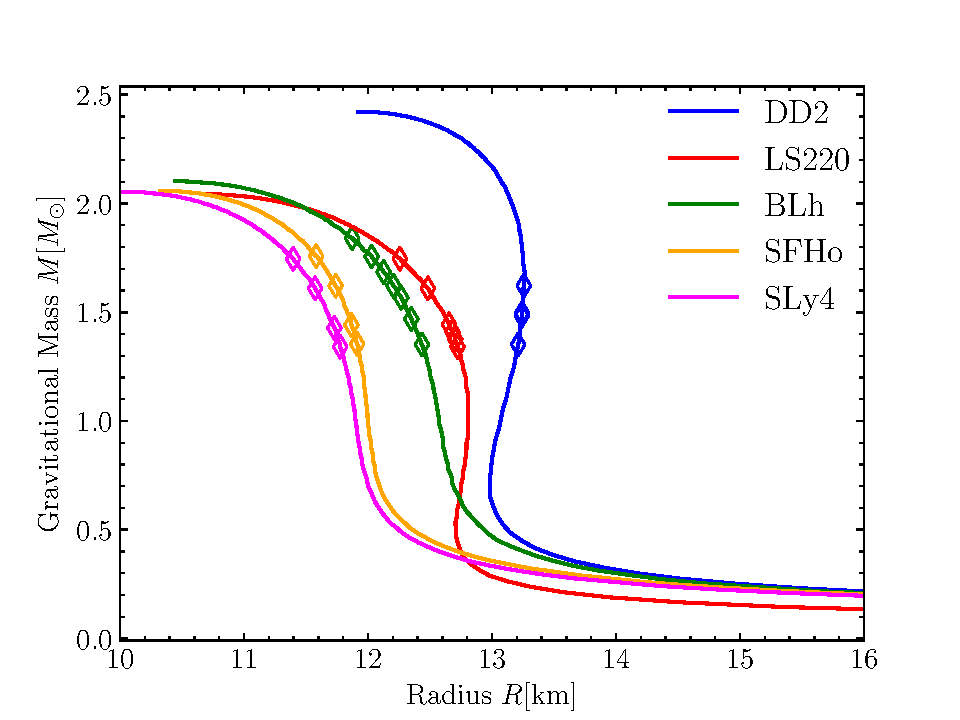
\includegraphics[width=0.49\textwidth]{tov_mr.pdf}
    \caption{Mass-radius relations for the EOSs used in this work. 
        Markers along the sequences indicate the NSs smulated in this work.}  
    \label{fig:method:tov_mr}
\end{figure}
%% 
To characterize these \acp{EOS}, that employs very different microphyscis and finite 
temperature properties and their relation to the electron fraction, we consider the \ac{TOV} solutions, 
presented on the Fig~\ref{fig:method:tov_mr}.
%
For cold, non-rotating \acp{NS}, these \acp{EOS} can support maximum 
masses in the range $\Mmax\sim 2.06-2.10\Msun$, while the predicted radii of a 1.4$\Msun$ 
NS lay in the range $R_{1.4}\sim 11.78-12.74$ km. 
More specifically, LS220, SFHo, SLy4, BLh and DD2 \ac{EOS} have 
$\Mmax$ of $2.04$, $2.06$, $2.06$, $2.10$ and $2.42$ $M_\odot$, and 
$R_{1.4}$ of $12.8$, $12.0$, $11.9$, $12.5$ and $13.2$ km respectively,.
%
These values are compatible, albeit in general lower, then those inferred from 
recent detection of an extremely massive millisecond pulsar \citep{Cromartie:2019kug} and with results obtained 
by the {\it NICER} collaboration \citep{Miller:2019cac,Riley:2019yda}.
Notably, \acp{EOS} that allow $R_{1.4}\gg 13$~km are currently disfavoured by both 
GW \ac{BNS} and X-ray pulsar observations \citep{Abbott:2018wiz,Miller:2019cac,Riley:2019yda}.
%
$\Mmax$ and $R_{1.4}$ related to the pressure at half saturation density \citep{Lattimer:2012nd}.
Thus we adopt the following naming convention for \acp{EOS}. Those that lead to a \ac{NS} with smaller 
radii are called "softer" and those that lead to a NS with larger radii are referred to as "stiffer" \acp{EOS}. 
Among considered, the DD2 \ac{EOS} is the stiffest, while SLy4 \ac{EOS} is the softest.

Finite temperature effects provides complimentary pressure support,
which is not sufficient to raise the maximum \ac{TOV} mass 
\citep{Kaplan:2013wra}, but can increase the radii of hot \acp{NS}.
Specifically, comparing the cold and hot ($s=2~{k_{\rm B}~{\rm baryon^{-1}}}$)
configurations, the thermal effects were shown to raise the $R_{1.4}$
by $15.6 \%$ for the LS220 EOS and $36.4 \%$ for the SLy4 EOS 
while for the BLh and the SFHo EOS the variation is $\sim 21-22 \%$.
%
Both \ac{NS} radius and maximum mass are increased if a \ac{NS} is rotating. 
For instance, at Keplerian limit, the maximum \ac{NS} mass is increased by 
$\sim 20\%$ for all \ac{EOS} models and radius by $\sim 40\%$ \citep{Bernuzzi:2020txg}. 
Naturally, rotation decreases the central density.
%
These observations highlight the importance of using full \acp{EOS} with finite-temperature effects. 

%% Thermal (and composition, see \citep{Kaplan:2013wra})
%% effects are indeed key to quantify the prompt collapse dynamics,
%% mass-shedding in the remnant and disc properties.




\section{Neutrino Radiation Transport}\label{sec:nr_methods:neut}

\red{Eq. for Q is needed as it is referenced in the results in Nu-wind}

During the neutron star mergers, the thermodynamic conditions are such that the powerful 
neutrino bursts can originate from the hot and shock heated NS matter \citep[\eg][]{Sekiguchi:2011zd}.
At high densities and temperatures reaching several MeV, the weak interaction become increasingly important,
moving the material away from the original chemical equilibrium with respect to the 
$\beta$-processes, and emission of numerous neutrinos with neutrino luminosity 
reaching $\sim10^{53}$erg s$^{-1}$ commences. 
% It was believed that such strong neutrino flux can power a \ac{GRB}, 
% however the baryon pollution of the polar region found in BNS simulations might make it 
% difficult \red{[refs, i think it was Perego work]}.

Neutrino transport is of prime importance for shaping the composition of the ejecta
\citep{Wanajo:2014wha,Sekiguchi:2015dma,Foucart:2015vpa,Foucart:2015gaa},
affecting the nucleosynthesis in the ejecta \citep{Wanajo:2014wha,Goriely:2015fqa} 
and the thermal electromagnetic counterpart, Kilonova (Macronova) \citep{Metzger:2014ila,Lippuner:2015gwa}

%%%% -----------------------------------------------------
%%%%         Introduction and Broad discussion  (From David and Others)
%%%% -----------------------------------------------------
%Neutrino interactions depend on the matter composition, its density and temperature, and on the neutrino energies. 
%For instance, at rest-mass density $10^{12}$\gcm and temperature $\sim10$~MeV, 
%the neutrino scattering on matter becomes so efficient, that they fall into the thermal equilibrium with it. 
%The mean free path of these neutrinos becomes of order of $\sim 50$~m. 
%These neutrinos are considered \textit{trapped}.
%At low densities, $<10^{11}$~\gcm, neutrinos with energy $<10$~MeV are no longer coupled to matter 
%and their mean free path can reach tens of kilometers. 
%Such neutrinos are considered \textit{free-streaming}.
%If there is a sharp density gradient present, \eg, a surface of a neutron star where density falls 
%by several orders of magnitude, then the neutrinos can be effectively divided into trapped and free-streaming. 
%The transition region, however, is more difficult to treat and requires more accurate neutrino treatment.
%%\textit{e.g.,} Monte Carly methods for solving Boltzmann equations \cite{Abdikamalov:2012zi}. Another alternative is the approximate, "ray-by-ray" \cite{Scheck:2007gw} multi-energy-group neutrino schemes [\textit{e.g.,} multi-group fluxlimited diffusion \cite{Mezzacappa:1993gn} and isotropic diffusion source approximation \cite{Liebendoerfer:2007dz}].
%
Radiation-transport equations are complex and expensive to solve numerically. 
%The main reasons for that are the following. First, is the high dimensionality of the problem. 
Radiation carriers are described by their location in space, which generally is comprised of $3$D space, momenta, 
which requires $2$ additional components, angles, and finally one component for energy of the carrier. 
Thus, with an addition of time there are $(6+1)$ dimensions for the problem. 
In addition, radiation transport depends strongly on the optical depth of the medium. 
If the latter is high, \ie, the opacity is very large, the radiation transport 
can be described by the diffusion of carriers, the formalism that have parabolic character. 
However, if the opacity is small and thus the optical depth, the radiation can stream freely, 
displaying a hyperbolic character of the transport \citep{Mihalas:1984}. 
%A particular difficulty is presented by the intermediate regime, when the radiation transport 
%mechanism transitions from diffusion to free streaming. 
%
Most commonly used approaches to simplify the radiation transport relies on reducing the diemnsionality
of the problem. In particular, -- reduce the number of spatial dimensions by assuming a certain symmetry.
%Examples are axial or spherical symmetry. And while this have shown to be a reasonable approximation for many astrophysical models, in cases where the system itself does not exhibit any spatial symmetries, 
%such simplification cannot be done. 
%%
Anther approach is to simplify the momentum space. 
%An example of such approach, that allows to reduce the computational cost considerably, is the approximation of transport equations with diffusion equations \citep{Pomraning:1973,Roe:1981}. 
%And while in the opaque regions (with high optical depth) this approximation is reasonable, it becomes much less 
%so in the transparent regions where the anisotropy of radiation has to be taking into account \citep{Ott:2008jb}.
%There, the free-streaming approximation is usually adopted. 
%%
%The solution in the intermediate region then obtained by the interpolating between the two. This approach can be augmented by using a two-moment schemes with analytic closures \citep[\eg][]{Brunner:2002}.
%However, in many applications a solution in all $(6+1)$ dimensions is a requirement.
%
%
The main source of complexity in the radiation transport stems from the scattering 
integral over all 4$\pi$ steradian.
By dividing the solid angle into a number of discrete angular intervals (rays), the integral can be replaced with a
finite sum, converting the integrodifferential equation into a linear system of equations for a multi-index object. 
%%
%This method of solving transport equation along several directions in each spatial zone the is called 
%discrete-ordinate ($S_n$) method \citep{Castor:2004,Ott:2008jb,Sumiyoshi:2012za,Godoy:2012}. 
%The discretization, however, comes with a a serious drawback, as it introduces regions which the 
%radiation cannot reach between the grid directions. 
%This is so-called "ray-effect" \citep{Morel:2003}, that causes large spatial oscillations in the transport variables.
%%
%\red{This method is a direct solution to Boltzmann eq}
%
%%A more physically motivated approximation to the radiation transport can be achieved by expending the radiation
%%It allows to convert the integrodifferential equation into a hyperbolic system of partial differential equations 
%%for the expansion coefficients. 
%%%
%%Coefficients stand for angular moments in the basis of spherical harmonic functions. 
%%An advantage of this method with respect to the diffusion approximation is that if in the latter 
%%the radaition propagation speed is unbound, in $P_N$ method, that approximates the radiation as a set of elementary
%%waves, the propagation speed is limited by the speed of light \citep{McClarren:2008b}.
%%%
%%This approach is also numerically more favorably, exhibiting the formal spectral convergence 
%%to the true solution and requiring less memory, a factor of two with respect to $S_N$ method for an 
%%equivalent angular distribution and accuracy. Preserving the rotational invariance, the $P_N$ method 
%%allows to avoid the "ray effect" of $S_N$ method. However, approximation of the radiation field with smooth 
%%basis functions, while being sufficiently accurate in the optically thick regime, displays non-physical 
%%oscillations in the transparent one \footnote{This is related to the so-called Gibbs phenomenon \cite{Boyd:2001}}.
%%If radiation is coupled to matter, these oscillations can produce regions with negative radiation intensity and 
%%thus negative temperature \citep{McClarren:2008b,Olson:2009} 
%%%
%%(see also \citet{Olson:2000,Olson:2009,Brunner:2001,McClarren:2010,Olson:2012,Hauck:2010}). 
%%%
%%One of the solutions to this problem is to filter out (using \eg, spherical spline expansion \citep{Boyd:2001}) 
%%these oscillations from the radiation intensity \citep{McClarren:2010}. However, the exact choice of the 
%%filtering technique, extension to full $3$D and absence of the clear continuum 
%%limit\footnote{Which does not allow to study the spatial convergence of the solution} 
%%present additional challenge in implementing the filtering approach. 
%
%
%Several methods are currently employed to study the neutrino radiaiton in 
%\ac{CCSN}, \ac{BNS} mergers and resulted \ac{BH}-torus systems.
%
%\begin{enumerate}
%    % ---
%    \item The simplest method to account for heating, cooling and deleptonization by neutrinos while not 
%    considering them directly, is to employ the \textbf{local source terms}, that describe the aforemntioned 
%    processes as functions of local thermodynamic quantities. This method was used in studes of shock-revival problem
%    in \ac{SN} \citep[\eg][]{Nordhaus et al., 2010; Hanke et al., 2011} and \ac{BNS} mergers \citep{Lee et al. (2005); Shibata et al. (2007)}.
%    % ---
%    \item A method that offers the simplicity of the 1 but also accounts for the optical depth of matter 
%    and geometry is the \textbf{leakage scheme} \citep{Ruffert et al. (1996); Rosswog \& Liebendorfer (2003); Kotake
%        et al. (2004); Sekiguchi (2010); O'Connor \& Ott (2010)}
%    It employs reasonable approximation to radiation transport is to consider the 
%    instantaneous energy loss via neutrino emission and evolution of the composition of the nuclear matter.
%    Neutrino leakage scheme was first proposed by \citet{vanRiper:1981mko} 
%    to study the neutrino cooling through weak interaction in the \ac{CCSN}.
%    Neutrino leakage scheme is popular to model neutrino effects in \acp{CCSN} and compact object mergers.
%    %
%    The scheme allows to estimate the effect of neutrino radiation transport, specifically tracking the 
%    evolution of the local lepton number and the association energy loss via neutrino radiation.
%    It has an advantage of being computationally efficient.
%    % ---
%    \item A more sophisticated method, that preserves the energy conservation, is the \textbf{flux-limited diffusion}
%    method. It has been widely adopted for \ac{CCSN} models of various dimensionalty and compelxity 
%    \citep{Bruenn et al., 1978; Bruenn, 1985)}.
%    The scheme's strengths include accuracy in the optically thick regions, computational efficiency and 
%    formulation, that hides the complexity of the underlying Boltzmann equation. 
%    However, by design, it relies on the specific way the transition to the optically thin regions is handled. 
%    Specifically, on the flux-limiting interpolation functions that prevent fluxes becoming superluminal. 
%    For \ac{BNS} mergers, a variant of this scheme, the multi-group (\ie, spectral) flux-limited diffusion 
%    was used by \citet{Dessart et al., 2009}.
%    % ---
%    \item In an attempt to tackle the problem of the radiation transport in different environments, the 
%    \textbf{isotropic diffusion source approximation} was derived \citep{Liebendorfer et al. (2009)}. 
%    The method splits the radiation field into the trapped part, treated via equilibrium-diffusion method, and 
%    a free-streaming part.
%    % ---
%    \item More accurate, \textbf{Boltzmann solvers}, are considerably more computationally expansive. 
%    As of now, their use is limited t othe so-called ray-by-ray approaches, that reduce the dimensionality 
%    of the problem, but may result in numerical artifacts. 
%    For instance, the state-of-the-art code for the \ac{CCSN} in 2D utilizes the ra-by-ray-plus method, where 
%    only the first two moments of the specific inteisty, (the energy denty and the flux desntiy) are evoloved.
%    This is so-called two-moment transport scheme \citep{Muller et al., 2010}.
%    Current state-of-the-art codes for the \ac{BNS} mergers also employ variations of two moment transport schemes 
%    \cite[\eg][]{Sekiguchi:2015dma}.
%    % ---
%    \item \textbf{Monte Carlo} is another way to solve the multidimensional radiation transport 
%    \citep{Fleck:1971,Gentile:2009,Abdikamalov:2012zi}. 
%    It can achieve very high accuracy, however, plague by the statistical noise 
%    (due to finite sampling of the phase space), they require very large number of Monte Carlo particles, 
%    and thus, they are computationally expensive. 
%\end{enumerate}
%%%% ---------------------------------------------------------------------------------


%% ---------------------------------------------------------
%% I N T R O  F R O M  J U S T  T H E S I S
%% ----------------------------------------------------------
%\paragraph{The equation of radiative transfer in the comoving frame}
%
%%% From Just PhD thesis
%
%Both, equations of \ac{HD} and for radiative transfer originate from \ac{BTE} for the respective frame
%independent particle distribution function \mathcal{F}, defined as 
%
%\begin{equation}
%    \dd N = \frac{g}{h^3}\mathcal{F}(\boldsymbol{x},\boldsymbol{p},t)\dd \boldsymbol{x} \dd \boldsymbol{p}
%\end{equation}
%
%where $\dd N$ is the number of particles in the phase space-space $\dd\boldsymbol{x}\dd\boldsymbol{p}$,
%$g$ is the statistical weight of the species and $h$ is the Plank's constant. 
%Under the ``radiation'', in this context, is implied the specific distribution of particles that move with the 
%speed of light and that are not influenced by external forces $\dot{\boldsymbol{p}}=0$.
%The \ac{BTE} in the fixed frame reads 
%
%\begin{equation}
%    \frac{1}{c}\frac{\partial}{\partial t} \mathcal{F} + \boldmath{n}\cdot\nabla_{x}\mathcal{F} = B,
%    \label{eq:theory:bte}
%\end{equation}
%
%where $\boldsymbol{n} = \boldsymbol{p}/|\boldsymbol{p}|$ and $B = B(\boldsymbol{x},\boldsymbol{p},t)$ 
%is the ``collision integral'' that in general has seven dimensions and includes explicit integrals in
%momentum space. Thus, Eq.~\eqref{eq:theory:bte} is the integro-partial differential equation.
%The quantity that is often used to discuss the frame dependent specific (\ie, monochromatic) intensity, 
%
%\begin{equation}
%    \mathcal{I}(\boldsymbol{x},\boldsymbol{n}, \epsilon, t) = (\epsilon/hc)^3 c \mathcal{F}(\boldsymbol{x},\boldsymbol{p},t)
%    \label{eq:theory:intensity}
%\end{equation}
%
%where $\epsilon = |\boldsymbol{p}|c$ is the energy. 
%Generally, the specific intensity $\mathcal{I}$ is measured in the frame comoving with the fluid, as the 
%collision integral, $B$, depends primarily on the particle distribution of the fluid part of the system.
%This is motivated by the fact that under the \ac{LTE}, the fluid distribution function becomes isotropic. 
%The symmetries allow to simplify the collision integral and makes it calculation more numerically 
%advantageous.
%%
%Next, we introduce the comoving-frame equation of radiation transport up to order 
%$\mathcal{O}(\upsilon/c)$ where $\upsilon=|\boldsymbol{\upsilon}|$ is the velocity of the fluid 
%measured in the lab frame. The laboratory or ``lab frame'' is a frame constructed from arbitrary but 
%fixed Eulerian coordinates. The equations read 
%\citep[\eg][]{Buchler, 1979; Kaneko et al., 1984; Munier & Weaver, 1986}
%
%\begin{equation}
%    \begin{aligned}
%    \frac{1}{c}\frac{\partial\mathcal{I}}{\partial t} + \frac{\boldsymbol{\upsilon}\cdot\boldsymbol{n}}{c^2}\frac{\partial\mathcal{I}}{\partial t} + n^j\frac{\partial\mathcal{I}}{\partial x^j} + \frac{\upsilon^j}{c}\frac{\partial\mathcal{I}}{\partial x^j} + \frac{\partial}{\partial \epsilon}\Big[ \mathcal{I}\epsilon \Big( \frac{\boldsymbol{a}\cdot\boldsymbol{n}}{c^2} + \frac{1}{c} n^j n^k \nabla_j\upsilon_k \Big) \Big] \\
%    + \frac{\partial}{\partial n^i}\Big[ \mathcal{I} \Big( \frac{\boldsymbol{a}\cdot\boldsymbol{n}}{c^2}n^i - \frac{a^i}{c^2} + \frac{1}{c}n^in^j\nabla_j\upsilon_k - \frac{1}{c}n^j\nabla_j\upsilon^i - k^i_{jk}n^jn^k - \frac{1}{c}\Gamma^{i}_{jk}\upsilon^j n^k \Big) \Big] \\
%    + \mathcal{I} \Big[ 2 \frac{\boldsymbol{a}\cdot\boldsymbol{n}}{c^2} \frac{1}{c}\nabla_i\upsilon^i + \Gamma^i_{ij}n^j + \frac{1}{c}n^i n^j\nabla_i\upsilon_j \Big] = C,
%    \end{aligned}
%    \label{eq:theory:bte_full}
%\end{equation}
%
%where $\boldsymbol{a} = \partial_t \boldsymbol{\upsilon}$, $\Gamma^i_{jk}$ are 
%Christoffel symbols associated with the spatial coordinates and $C = (\epsilon/hc)^3 c B$.
%Equation Eq.~\eqref{eq:theory:bte_full} can be obtained from Eq.~\eqref{eq:theory:bte}, using 
%Eq.~\eqref{eq:theory:intensity} and the $\mathcal{O}(\upsilon/c)$ variant of the Lorentz 
%transformations for $\mathcal{I}$, $\epsilon$, and $\boldsymbol{n}$.


\subsection{Neutrino leakage scheme}

\red{Introduce electron fraction, \&
beta equilibrium condition
}

\begin{table}
    \caption{
        Weak reactions employed in our simulations and references for their implementation.
        In the left column, $\nu \in \{\nu_e, \bar{\nu}_e, \nu_{x}\}$ denotes any neutrino species, 
        $\nu_{x}$ any heavy-lepton neutrinos, $N \in\{n, p\}$ a nucleon, and $A$ any nucleus.
        In the central column the role of each reaction is highlighted with "P" standing for 
        production, "A" for absorption opacity and "S" for scattering opacity.
        When two roles are included, the second refers to the inverse ($\leftarrow$) reaction.
        Table is taken from \citet{Radice:2018pdn}.
    }
    \label{tab:leakage}
    \begin{center}
        \begin{tabular}{l l l}
            \hline\hline
            Reaction & Role &  Ref. \\ 
            \hline
            $p + e^- \leftrightarrow \nu_e + n $          & P,A & \citep{Bruenn:1985}  \\
            $n + e^+ \leftrightarrow \bar{\nu}_{e} + p $  & P,A & \citep{Bruenn:1985}  \\
            $e^+ + e^- \rightarrow \nu + \bar{\nu}$       & P   & \citep{Ruffert:1995fs} \\
            $\gamma + \gamma \rightarrow \nu + \bar{\nu}$ & P   & \citep{Ruffert:1995fs} \\
            $N + N \rightarrow \nu + \bar{\nu} + N  + N$  & P   & \citep{Burrows:2004vq} \\
            $\nu + N \rightarrow \nu + N$                 & S   & \citep{Ruffert:1995fs} \\
            $\nu + A \rightarrow \nu + A$                 & S   & \citep{Shapiro:1983du} \\
            \hline\hline
        \end{tabular}
    \end{center}
\end{table}

For numerical reasons, the neutrino transport in the optically thick region, 
where radiation and matter are coupled, is handled the so-called ``leakage scheme''. 
The method accounts for the optical depth of matter and geometry 
\citep{Ruffert:1995fs,Rosswog:2003rv,Sekiguchi:2010zz,OConnor:2009iuz,Galeazzi:2013mia}
%
For other implementations and methods see \eg, 
\citet{vanRiper:1981mko,Ruffert:1995fs,Rosswog:2003rv,OConnor:2009iuz,Sekiguchi:2010ep,
    Neilsen:2014hha,Perego:2015agy,Ardevol-Pulpillo:2018btx}.
%
The method approximates the radiation transport evaluating the instantaneous energy loss 
via neutrino emission and evolution of the composition of the nuclear matter.
The particular advantage of the method is its computational efficiency and an ability 
to account for non-trivial geometries of emitting regions.
%
It was first proposed by \citet{vanRiper:1981mko} to study the neutrino cooling through weak interaction 
in the \ac{CCSN}. The leakage scheme is popular to model neutrino effects in \acp{CCSN} 
and compact object mergers.
%
A modified version of \cite{Galeazzi:2013mia} scheme is implemented in 
\ac{NR} code \wisky{} \citep{Radice:2016dwd,Radice:2018pdn}.

%Non-equilibrium weak-interaction processes lead to the production of numerous neutrions 
%from the hot, dense and neutron-rich matter, \textit{e.g.,} BNS merger remnant. 
%The cooling effect associated with the neutrino emission, that could cause dynamical 
%instabilities, is important for the structure and evolution of the remnant. 
%To evaluate the influence of thermal effects on the onset of dynamical instabilities, the long-term evolution, (several dynamical timescales of the object with $M$ mass and $R$ size $\tau_{\text{dyn}}\sim(M/R^3)^{1/2}\approx 1$~ms) is required.

%
The goal of the scheme is to describe a series of effective emissivities, 
$R_{\nu}^{\text{eff}}$, and $Q_{\nu}^{\text{eff}}$ for electron neutrinos, $\nu_e$, 
anti-electron neutrinos $\bar{\nu}_e$ and the heavy-lepton neutrinos, 
which are collectively labeled as $\nu_x$.
Here $R_{\nu}^{\text{eff}}$ describes the the number of neutrinos emitted per second and baryon,
and $Q_{\nu}^{\text{eff}}$ describes the energy emitted via neutrinos per second and baryon.
%
Then, the optical depth is evaluated and used to reduce the intrinsic emissivites, 
mimicking the effect of the diffusion of radiation from the optically thick regions.
%\red{This scheme also includes the heating effects by the free-streaming neutrinos, \textit{i.e.,} neutrino absorption}. \gray{ which was shown to be important for altering the ejecta composition }.
%
%The following neutrino species are considered: electron neutrino, $\nu_e$, 
%(and its anti-neutrino $\bar{\nu}_e$) and heavy lepton neutrino $\nu_{\tau,\mu}=\nu_X$ (and its antineutrino). %\gray{that are a single component with statistical weight of 4.}.
%
Neutrinos are assumed to be massless and in thermal equilibrium with the surrounding matter.
%As a result, the energy spectrum of the neutrinos follows a Fermi-Dirac distribution for
%ultrarelativistic particles at the temperature of the matter. 
%The chemical potential $\nu_e$ and $\bar{\nu}_e$ is assumed to the at equilibrium, \cite{Rosswog:2003rv},
%
%\begin{equation}
%\mu_{\nu_e}^{\text{eq}} = \mu_e - \mu_n - \mu_p = -\mu_{\bar{\nu}_e}^{\text{eq}}
%\end{equation}
%
%where $\mu_e$, $\mu_n$, $\mu_p$ are the relativistic chemical potentials including the rest-mass of the particle. 
The $R_{\nu}^{\text{eff}}$, and $Q_{\nu}^{\text{eff}}$ can be evaluated from various 
weak-interaction processes present in the hot and dense matter of the NS. 
%The definitions are: the $Q_{\nu_{i}}$ is the energy emitted via neutrinos per second and baryon;
%the $R_{\nu_{i}}$ is the number of neutrinos emitted per second and baryon.
%%
%The most important neutrino emission processes in the NS remnant are: 
%\begin{itemize}
%    \item electron and position capture on nucleons, the $\beta$-process,
%    \item electron-positron pair annihilation, 
%    \item transverse plasmon decay.
%\end{itemize}
%
The reactions considered with in the scheme, implemented in \wisky{} are listed in the 
Tab.~\ref{tab:leakage}.
%
It is possible to evaluate the emission rates corresponding to these processes 
using only the quantities provided by the \ac{EOS} tables.

%%%% === URCA PROCESS
For instance, consider the strong neutrino emitting process, the direct Urca process, 
that consists of the $\beta$-decay, $e^+ + n \rightarrow p + \bar{\nu}_e$ 
and the electron capture on the free nucleons (n), $e^{-} + p \rightarrow n + \nu_e$ 
(the first two reactions Tab.~\ref{tab:leakage}). 
This process moves the matter to the $\beta$-equilibrium, in which the rats 
of both reactions are the same, and the chemical potentials $\mu_{\nu_e,\bar{\nu}_e}=0$.
%
For both, $\beta$-decay, ``\text{pc}'', and electron capture, ``\textit{ec}'', the 
\begin{equation}
\begin{aligned}
    Q_{pc}(\bar{\nu}_e) &= n_b^{-1}\beta\eta_{pn}T^6F_5(-\eta_e)[1-f_{\bar{\nu}_e}]_{pc} \\
    Q_{ec}(\nu_e) &= n_b^{-1}\beta\eta_{np}T^6F_{5}(\eta_e)[1-f_{\nu_e}]_{ec}
\end{aligned}
\label{eq:theory:qecpc}
\end{equation}
and
\begin{equation}
\begin{aligned}
    R_{pc}(\bar{\nu}_e) &= n_b^{-1}\beta\eta_{pn}T^5F_4(-\eta_e)[1-f_{\bar{\nu}_e}]_{pc} \\
    R_{ec}(\nu_e) &= n_b^{-1}\beta\eta_{np}T^5F_{4}(\eta_e)[1-f_{\nu_e}]_{ec}
\end{aligned}
\label{eq:theory:recpc}
\end{equation}
where $T$ is the temperature, $n$ are the number densities, $\eta=\mu/T$ with $\mu$ being the 
chemical potential, $F_N$ are the Fermi integrals of order $N$,
$1-f_{\nu}$ is a factor related to the Fermi-Dirac distribution, $f_{\nu}$, and $\beta$
is a constant \citep{Bruenn:1985}.
%
Equations Eq.~\eqref{eq:theory:qecpc} and \eqref{eq:theory:recpc} display a strong dependency 
of neutrino production on temperature.
%
%$Q_{\text{pc}}(\bar{\nu}_e),Q_{\text{ec}}({\nu_e}) \propto T^{6}$ 
%while 
%$R_{\text{pc}}(\bar{\nu}_e),R_{\text{ec}}(\nu_e)\propto T^5$, 
%
%At high temperatures but moderate densities, the plasmon decay is one of the major sources of neutrinos, 
%where the plasmon is the quanta of electromagnetic field in plasma exhibiting two polarizations, 
%among which only the tansverse polarisation is important in this context.
%\cite{P. J. Schinder, D. N. Schramm, P. J.Wiita, S. H. Margolis, and D. L. Tubbs, Astrophys. J. 313, 531 (1987).} 
%\red{But I am not sure that plasmon decay in included in the Leackage scheme on Whisky}


%%% ==== SCATTERING
In addition to the emission of neutrinos, the leakage scheme considers the neutrino absorption and scattering, 
(see "A" and "S" entries in the Tab.~\ref{tab:leakage}, $\nu+A\rightarrow\nu+A$ is the coherent neutrino 
scattering on heavy nuclei (with atomic mass number $A$), and $\nu+N\rightarrow\nu+N$ 
is the neutrino scattering on free nucleons).
%
Of particular importance are the neutrino scattering on heavy nuclei, and on free nucleons, 
as well as electron-flavor neutrinos absorption on free nucleons. 
The mathematical formulation of these opacities see \citet{Galeazzi:2013mia} and their Appendix A.
%
The neutrino scattering on nuclei becomes the dominant opacity source when the heavy neuclei 
are abundant, nuclei that form below nuclear saturation density ant low temperatures $<15$~MeV \citep{Rosswog:2003rv}.

Taking the considered scattering and absorption processes, the local mean free-path for each neutrino species 
can be computed. From it, the energy-independent mean free path can be derived, that in turn depends 
only on the local thermodynamic condition. 
This allows to evaluate the energy-independent part of the optical depth and diffusion rates.
%
The optical depth allows to asses the extend of the optically thick region 
(that is neutrino-species dependent) and it allows to asses the time needed for neutrinos to 
diffuse out of the dense matter, diffusion timescales.. 
%It should be noted that for cores of a neutron star this diffusion timescale is of order of seconds. 
%Thus, neutrinos that are expected to contribute the most on the dynamical timescale are the nuetirnos abundantly
%emitted at the \textit{neutrinosphere} and above \citep{Galeazzi:2013mia,Endrizzi:2018uwl}.
%
%\red{The diffusive number and energy emission rates per baryon are 'interpolated' 
%    between diffusive and free-streaming regimes.
%    So it seems that both, diffusion rates and free neutrino emission rates per baryon are computed here, using the ioptical depth to separate them. Then, the effective rates are computed via interpolation.
%}

%A quatity that is op particular usefullness for describing neutrino cooling  is the neutrinosphere,
%defined as \cite{Galeazzi:2013mia}
%\begin{equation}
%\frac{Q_I}{Q_{I}^F} = \frac{2}{3}
%\end{equation}
%where $Q_I$ is the interpolated effective emission rate, $Q_I^F$ is the neutrino luminosity per baryon.
%The neutrino cooling is suppressed inside this region, and the neutrino escape timescale is the diffusion timescale. 
%The neutirnosphere is however can also be defined as $\tau=2/3$, \textit{e.g.,} \cite{Rosswog:2003rv,Endrizzi:2018uwl}.
%After the interpolation, the net net emission rate per baryon appearing $\mathcal{R}$ and and the luminosity per baryon $\mathcal{Q}$.
%
%Importantly, the assumption of the chemical equilibrium can lead to an overestimation of the neutrino emission rates in the transition region, etween the optically thin and thick.

%%%%% ==== from Radice2018pdn >>>
%
%Alongside the neutrino production rate, $R_{\nu}$, and respective energy release, $Q_{\nu}$, for 
%$\nu\in\{\nu_e,\bar{\nu}_e,\nu_x\}$, the opacities, $\kappa_{\nu;a}$ and $\kappa_{\nu;s}$ 
%for absorption and scattering respectively are evaluated, where the 
%thermodynamical equilibrium chemical potential is assumed for neutrinos.
%
The opacities are split into two types. The density weighted opacities $\kappa_{\nu;a}^0$ and
$\kappa_{\nu;s}^0$ and energy density weighted opacities $\kappa_{\nu;a}^1$ and $\kappa_{\nu;s}^1$. 
The former are related to the rate at which neutrinos escape the material, 
while the latter set the rate at which energy escapes the material as neutrinos escape 
\citep{Ruffert:1995fs}.
%
The optical depth, $\tau_{\nu}^{\alpha}$ is computed taking into account 
total neutrino opacities $\kappa_{\nu;a}^j + \kappa_{\nu;s}^j$ \citep{Neilsen:2014hha}.
%
Optical depth is then used to estimate the effective emission rates \citep{Ruffert:1995fs} as 
%
\begin{equation}
R_{\nu}^{\text{eff}} = \frac{R_{\nu}}{1 + t_{\text{diff}}^0(t^0_{\text{loss}})^{-1}}
\label{eq:method:whisky:Rnueff}
\end{equation}
%
where $t_{\text{diff}}$ and $t_{\text{loss}}$ are the neutrino diffusion time and emission timescales,
%
\begin{equation}
t_{\text{diff}}^{0} = \mathcal{D}\frac{(\tau_{\nu}^0)^2}{\kappa_{\nu;a}^0 + \kappa_{\nu;s}^0}, \hspace{5mm} t_{\text{loss}}^0 = \frac{R_{\nu}}{n_{\nu}},
\end{equation}
%
%and the neutrino emission timescale 
%
%\begin{equation}
%t_{\text{loss}}^0 = \frac{R_{\nu}}{n_{\nu}}
%\end{equation}
%
and $n_{\nu}$ is the neutrino number density estimated based on the 
beta equilibrium with neutrinos and \red{$\tau_{\nu}$ is the optical depth}.
The $\mathcal{D}$ is a tuning parameter set to $6$ \citep{Radice:2018pdn}.
%
Similarly, the effective energy emission rate $Q_{\nu}^{\text{eff}}$ 
is computed with $\tau_{\nu}^1$, $\kappa_{\nu;a}^1$ and $\kappa_{\nu;s}^1$.

%Notably, the effect of trapped neutrinos was shown to be weak in the \ac{NS} conditions 
%\citep{Galeazzi:2013mia} and thus neglected here.
The neutrinos that escape according to the effective rate $R_{\nu}^{\text{eff}}$,
with the average energy $U_{\nu}^{\text{eff}}/R_{\nu}^{\text{eff}}$ 
are the free streaming neutrinos $n_{\nu}^{\text{fs}}$. 
%
These neutrinos are treated afterwards according to the 
M0 scheme in the optically thin region \citep{Radice:2016dwd}.

%% ----------------------------------
%%%% from Galezzi:2013 again
%% ----------------------------------
%Note that the total neutrino luminocity is an observer dependent quantity in relativity. 
%The reason is that the the neutrino energy emitted at a given point between coordinate times $t$ and $t+dt$, 
%which are measured by the coordinate observer with world line tangent to $t^{\mu}$. 
%Further assumption of stationarity is then required, \eg, assuming $t^{\mu}$ is the Killing vector. 
%Then, the neutrino energy at infinity is $E_{\nu}^{\infty} = \sqrt{-g_{00}}E_{\nu}$, 
%irrespective of the direction of emission.
%
%Summarizing, since (trapped) neutrinos are assumed to be in equilibrium with the baryonic matter, the number density and energy distribution of neutrinos is not evolved -- their contribution to the source terms 
%$\Psi^{\beta}$ 
%$Qu^{\mu}$ and 
%$N$ 
%$R_{p,n}$
% is obtained from the matter properties.

%\gray{only the electron neutrinos are considered there, and only their degrees of freedom is accounted for by the electron fraction $Y_e=n_e/n_b$.
%    The electron fraction is changed only by the neutrinos (antineutrinos) according to the source term $N$.}

%\gray{Galezzi:13:
%    pressure and specific internal energy contain contributions of baryons, electrons, photons and trapped neutrinos
%    \begin{align}
%    p &= p_e + p_b + p_{\gamma} + p_{\nu_e,\bar{\nu}_e}... \\
%    \epsilon &= \epsilon_e + \epsilon_b + \epsilon_{\gamma} + \epsilon_{\nu_e,\bar{\nu}_e} + ...
%    \end{align}
%    where the contribution from trapped electron-neutrinos $\nu_e$ and
%    antineutrinos $\bar{\nu}_e$ in the dense baryonic component can be evaluated from the thermodynamic state of the fluid and assuming that the neutrinos are following a Fermi-Dirac distribution 
%    \begin{align}
%    p_{\nu_e,\bar{\nu}_e} &= p_{\nu_e} + p_{\bar{\nu}_e} = \frac{4\pi}{3}T^4[F_3(\eta_{\nu_e}) + F_3(\eta_{\bar{\nu}_e})], \\
%    \epsilon_{\nu_e,\bar{\nu}_e} &= \epsilon_{\nu_e} + \epsilon_{\bar{\nu}_e} = \frac{1}{3}\frac{p_{\nu_e,\bar{\nu}_e}}{\rho}
%    \end{align}
%    where $\eta_{\nu_e} = \mu_{\nu_e}/T$ and $\eta_{\bar{\nu}_e} = \mu_{\bar{\nu}_e}/T$ are the degeneracy parameters for the electron-neutrinos and antineutrinos, $\mu_{\nu_e}$, $\mu_{\bar{\nu}_e}$ the corresponding chemical potentials and $T$ is the temperature, $F_3(\eta_{\nu_e})$ is the Fermi integral.
%    There, the contributions of trapped neutrinos to pressure and internal energy is neglected, 
%    $p_{\nu_{e},\bar{\nu}_e}=\epsilon_{\nu_e,\bar{\nu}_e}=0$.
%    For the computation of the neutrino source term $N$, the neutrinos emission rates per baryond are introduced $R_{\nu_e}$ and $R_{\bar{\nu}_e}$ for electron neutrinos and antineutrinos respectively. Then in the fluid rest-frame the change in electrom fraction is $u^{\alpha}\nabla_{\alpha}(Y_e)=\matcal{R} = R_{\bar{\nu}_e} - R_{\nu_e}$. 
%    Similarly, for the source term $\Psi^{\beta}$ that describes the radiative losses of energy and momentum due to neutrinos, the neutrino emissivity $Q$ is intorcued. Assumptions: emission is isotropic in the fluid's rest frame. Then the covarient equation reads 
%    \begin{equation}
%    \Psi^{\beta} = -\rho m_b^{-1}Qu^{\beta} = \rho m_b^{-1}\sum_I Q_I u^{\beta} = -\rho m_b^{-1} (Q_{\nu_e} + Q_{\bar{\nu}_e} + Q_{\nu_{\tau,\mu}}+Q_{\bar{\nu}_{\tau,\mu}})u^{\beta}
%    \end{equation}
%    Here, the emissivity due to the $\tau$ and $\mu$ neutrinos into a single contribution $ Q_{\nu_{\tau,\mu}}$.
%    These equations, for numerical evolution, the equations are cast into a flux conservative formulation, based on the Valencia formulation, representing Eurler equtions and lepton/baryon number conservations as balance laws.
%    \begin{equation}
%    \partial_t (\sqrt{\gamma}\boldsymbol{q}) + \partial_t\Big( \sqrt{\gamma} \boldsymbol{f}^{(i)}(\boldsymbol{q}) \Big) = s(\boldsymbol{q}).
%    \end{equation}
%    where $\gamma$ is the determinant of the three-metric, while $\boldsymbol{f}^{(i)}(\boldsymbol{q})$ and $s(\boldsymbol{q})$ are the flux vectors and source terms, respectively \cite{Font:2008fka}.
%}

%The foundation of the scheme described here is presented in \cite{Galeazzi:2013mia}.
%The method is similar to that of the \cite{Ruffert:1995fs}.
%And, as in the \cite{Rosswog:2003rv}, the opacities are computed on the basis local thermodynamical equilibrium chemical potential for the neutrinos.


%The scheme consideres three neutrino species: electron neutrino $\nu_e$, electron antineutrino $\bar{\nu}_e$ and an single species $\nu_x$ for heavy-lepton neutrinos.
%The reactions traced by the scheme are listed in the table \ref{tab:leakage}.



%\gray{
%    Notably, the $E == n_{\alpha}n_{\beta}T^{\alpha\beta}$, 
%    $S_i = -\gamma_{i\alpha}n_{\beta}T^{\alpha\beta}$ and $S_{ij} = \gamma_{i\alpha}\gamma_{j\beta}T^{\alpha\beta}$ are the matter source terms where $n_{\alpha}=(-\alpha, 0, 0, 0)$ is the future pointing four-vector orthonormal to the space-like hypersurface, $S=S_{i}^{i}$ is the trace.
%}






\subsection{Neutrino M0 scheme}

%% === From Just thesis
%In order to describe the interaction of free-streaming neutrinos effects with matter a variant of the 
%Boltzmann solver is required. In the following we consider a particular technique, 
%commonly referred to as a variable Eddington factor technique, that is based on the evolution 
%of the set number of moments of the specific intensity. 
%For instance, if the number is two, namely, the
%energy density and flux density are evolved, such scheme is called two-moment transport scheme.
%There the second moment, the Eddington factor is obtained in a separate procidure via solving 
%the simplified Boltzmann equation \citep{(e.g. Mihalas & Mihalas, 1984)}.
% -------------------------

The free-streaming neutrinos are treated via a variant of the moment equations of energy transport, 
the M0 scheme \citep{Radice:2016dwd,Radice:2018pdn}.
Computation of the neutrino number density and energy is 
%$n_{\nu_e}$, $n_{\bar{n}_e}$, $E_{\nu_e}$ and $E_{\bar{\nu}_e}$ is 
accomplished via the zeroth momentum (M0) of the free-streaming neutrino distribution 
function on a set of individual radial rays, with the closure adopted to the post-merger geometry.

%% M0 Appendix A from Radice:2016dwd, Neutrin transport details
%\subsubsection{The Boltzmann equations for Free-Streaming Neutrinos}
%First, the Boltzmann equation is derived for the neutrinos, that are again assumed to be massless 
%particles. 
Neutrinos propagate in the fluid with four-velocity is $u^{\alpha}$ and four-momentum, $p^{\alpha}$.
The latter can be decomposed as \citep{Thorne:1981}
%
%% \begin{equation}
$p^{\alpha} = (-p_{\beta}u^{\beta})(u^{\alpha} + r^{\alpha})$, 
%% \end{equation}
%
where $E_{\nu}=-p_{\alpha}u^{\alpha}$ is the neutrino energy measured by Eulerian observer,
comoving with the fluid, $r^{\alpha}$ is the unit space-like vector, orthogonal to the 
fluid's $u^{\alpha}$, or in other words $r_{\alpha}r^{\alpha}=1$ and $u_{\alpha}r^{\alpha}=0$.
%
Additionally, $r^{\alpha}$ can be interpreted as the direction along which neutrinos move,
as seen by the Eulerian observer comoving with the fluid.
%
The four-vector of the neutrinos is
%
%% \begin{equation}
%% \label{eq:method:whisky:neut:k}
$k^{\alpha} = u^{\alpha} + r^{\alpha}$ 
%% \end{equation}
%
with $k_{\alpha}k^{\alpha} = 0$ normalized such that $k^{\alpha}u_{\alpha}=-1$.
%
Next, the affine parameter, $l$, that parameterizes the neutrino's worldline is introduced
%
%% \begin{equation}
%% l = \int (-p_{\alpha u^{\alpha}})\dd s \text{ so that } \Big( \frac{\partial}{\partial l} \Big)^{\alpha} = %% k^{\alpha}.
%% \end{equation}
% 
such that $(\partial / \partial l)^{\alpha} = k^{\alpha}$.
%
Now, with $l$, the Boltzmann equations for the neutrino radiation transport read \citep{Thorne:1981}
%
\begin{equation*}
\frac{D F}{D l} = \mathbb{C}[F],
\end{equation*}
%
where $F$ is the distribution function for a give neutrino species, and $\mathbb{C}$ is the
``collisional operator'' that contains information regarding the interactions 
between neutrinos and the background fluid (in the frame of the fluid. 
%
The $D/Dl$ is the total derivative in phase space along $p^{\alpha}$ and it reads 
%
\begin{equation}
\label{eq:method:whisky:neut:bolzeq}
\frac{DF}{Dl} = k^{\alpha} \Big[ \frac{\partial F}{\partial x^{\alpha}} - \Gamma^{\delta}_{\:\:\alpha\beta}p^{\beta}\frac{\partial F}{\partial p^{\delta}} \Big],
\end{equation}
%
where $\Gamma^{\delta}_{\:\:\alpha\beta}$ are the Christoffel symbols.
%
%\subsubsection{Neutrino number density evolution}
%Neutrinos are split into two categories. 
%Trapped neutrinos are treated with leackage scheme.

The obtained Boltzmann equation, Eq.~\eqref{eq:method:whisky:neut:bolzeq}, allows to describe
the evolution of the free-steaming neutrinos and track the evolution of their average energy.
%
The source term is computed taking the effective emissivities from the leakage scheme.
The collisional term is approximated in a way that it only includes neutrino absorption and emission. 
Scattering is neglected.
For the evaluation of the absorption opacities, (of $\nu_{e}$ and $\bar{\nu}_{e}$) the 
\ac{LTE} is assumed.
The neutrinos are assumed to propagate along the radial rays. 
\citep{Radice:2016dwd,Radice:2018pdn}.

%%%% ---------------------------
%% On the Balance Eqution and Closure
%%%% ---------------------------
%The neutrino number density (in the fluid rest frame) for neutrinos of a give flavor, $n_X$, 
%can be expressed through the neutrino number current $J_{X}^{\alpha}$ that reads \citep{Lindquist:1966},
%%
%\begin{equation}
%J_{X}^{\alpha} = \int F p^{\alpha} \frac{\dd^3 p}{-p_0}
%\end{equation}
%%
%as $n_X = - u_{\alpha} J_{X}^{\alpha}$.
%%
%The balance equation (between absorption and emission of neutrinos) can be obtained from the 
%first moment of the Boltzmann equation \cite{Thorne:1981,Shibata:2011kx}
%%
%\begin{equation}
%\label{eq:method:whisky:neut:balanseq}
%\nabla_{\alpha}J_{X}^{\alpha} = R_{X}^{\text{eff}} - \kappa_X n_X,
%\end{equation}
%%
%where $\kappa_X$ is the absorption opacity and $R_X^{\text{eff}}$ is the effective neutrino emission rate.
%%
%While the equation Eq.~\eqref{eq:method:whisky:neut:balanseq} is exact, in order to be solved, 
%it requires closure. 
%In this method the closure is given by considering neutrinos only 
%propagating radially and at a speed of light, \eg, 
%%
%%% \begin{equation}
%$J_{X}^{\alpha} = n_X k^{\alpha}$, 
%%% \end{equation}
%%
%where $k^{\alpha}$ is the fiductial null vector from 
%$k^{\alpha} = u^{\alpha} + r^{\alpha}$ %% \eqref{eq:method:whisky:neut:k}, 
%under the assumption that $r^{\alpha}$ is the radial null-vector, orthogonal to the fluid $u^{\alpha}$.
%%This translates into the assumption that the free-streaming neutrinos are 
%%moving radially in a frame instantaneously comoving with the fluid.
%%
%Then, the balance equation for $n_X$ reads
%%
%\begin{equation}
%\label{eq:mehtod:whisky:neut:balanseq2}
%\partial_t(\sqrt{-g}n_X k^t) + \partial_r(\sqrt{-g}n_X k^r) = \sqrt{-g}(R^{\text{eff}}_{X} - \kappa_X n_X)
%\end{equation}
%%
%where $g$ is the determent of the $4$-metric \gray{(in spherical coordinates)}.
%%%% -------------------------------------

The balance equation (between absorption and emission of neutrinos) can be obtained from the 
first moment of the Boltzmann equation \citep{Thorne:1981,Shibata:2011kx}
%\begin{equation}
%\label{eq:theory:neut:balanseq1}
%\nabla_{\alpha}J_{X}^{\alpha} = R_{X}^{\text{eff}} - \kappa_X n_X,
%\end{equation}
%\begin{equation}
%\label{eq:theory:neut:balanseq1}
%\partial_t(\sqrt{-g}n_X k^t) + \partial_r(\sqrt{-g}n_X k^r) = \sqrt{-g}(R^{\text{eff}}_{X} - \kappa_X n_X)
%\end{equation}
%
%where $n_X$ is the number density, 
%$\kappa_X$ is the absorption opacity and $R_X^{\text{eff}}$ 
%is the effective neutrino emission rate.
%
The closure is achieved by considering neutrinos propagating only radially with the 
speed of light, $\partial_t$ is a Killing vector. 
Then the free-streaming neutrino energy satisfies \cite{Radice:2016dwd,Radice:2018pdn}.

\begin{subequations}
    \begin{align}
        \partial_t(\sqrt{-g}n_X k^t) + \partial_r(\sqrt{-g}n_X k^r) &= \sqrt{-g}(R^{\text{eff}}_{X} - \kappa_X n_X) \label{eq:theory:neut:balanseq1} \\
        k^t\partial_t(E_{\nu}^{\text{fs}}\chi) + k^r\partial_r(E_{\nu}^{\text{fs}}\chi) &= \frac{\chi}{n_{\nu}^{\text{fs}}} (Q_{\nu}^{\text{eff}} - E_{\nu}^{\text{fs}}R_{\nu}^{\text{eff}}) \label{eq:theory:neut:balanseq2} 
    \end{align}
\end{subequations}

where $n_X$ is the number density, $\chi=-k^{\alpha}(\partial_t)_{\alpha}$
$\kappa_X$ is the absorption opacity and $R_X^{\text{eff}}$ 
is the effective neutrino emission rate.

%\begin{equation}
%\label{eq:theory:neut:balanseq2}
%\partial_t(\sqrt{-g}n_X k^t) + \partial_r(\sqrt{-g}n_X k^r) = \sqrt{-g}(R^{\text{eff}}_{X} - \kappa_X n_X)
%\end{equation}
%
%\begin{equation} %% Eq 9 from 2018pdn
%    \label{eq:theory:neut:balanseq2}
%    k^t\partial_t(E_{\nu}^{\text{fs}}\chi) + k^r\partial_r(E_{\nu}^{\text{fs}}\chi) = \frac{\chi}{n_{\nu}^{\text{fs}}} (Q_{\nu}^{\text{eff}} - E_{\nu}^{\text{fs}}R_{\nu}^{\text{eff}})
%\end{equation}
%
%
%The equation Eq.~\ref{eq:theory:neut:balanseq2} is then solved 
%numerically on a series of 
%independent radial rays at every timestep of the evolution.

%%%% --------------------------------------------
%% Neutrino average energy evolution
%%%% --------------------------------------------
%Next, the computation of the neutrino average energy is 
%required to evaluate the matter composition and temperature changes.
%%
%Here the additional assumption is made, that the space-time is stationary, \eg, 
%$t^{\alpha}:=(\partial_t)^{\alpha}$ is a Killing vector, which leads to the 
%$(-p_{\alpha}t^{\alpha})$ to be a conserved quantity.
%%
%% Assuming that there is no interaction with the fluid and the along the neutrino worldlines, \eg, 
%%
%%% \begin{equation}
%%% $\frac{\dd(-p_{\alpha}t^{\alpha})}{\dd l} = 0$
%%% \end{equation}
%% $\dd(-p_{\alpha}t^{\alpha} / \dd l = 0$, 
%
%Then, the quantity $\mathcal{E}_X = -p_{\alpha}t^{\alpha}$ is the energy of the neutrinos 
%of species $X$ as sees by the coordinate observer\footnote{
%    an unphysical observer with four-velocity $t^{\alpha}$
%}.
%
%%% --- MIGHT be a repetition
%%Consider 
%%
%%\begin{equation}
%%    \mathcal{E}_X = -p_{\alpha}t^{\alpha} = -E_{X} k_{\alpha}t^{\alpha} =: E_X \chi
%%\end{equation}
%%
%%then, the equation for the average neutrino energy reads
%%
%%\begin{equation}
%%    \frac{\dd \mathcal{E}_X}{\dd l} = \frac{R^{\text{eff}_X}}{n_X}\Big( \chi \frac{Q_X^{\text{eff}}}{R_{X}^{\text{eff}}} - \mathcal{E}_X \Big) 
%%\end{equation}
%%
%%where $Q_{X}^{\text{eff}}$ is the effective neutrino energy source (taken from the leakage scheme).
%%
%%For neutrinos radially moving, the equation reads
%%
%%\begin{equation}
%%    n_X k^{t} \partial_t \mathcal{E}_X + n_{X} k^{r}\partial_{r}\mathcal{E}_X = (\chi Q_{X}^{\text{eff}} - \mathcal{E}_X R_X^{\text{eff}}).
%%\end{equation}
%%
%%This eqution is solved on the same spherical grid using hte first order finite differencing method.
%
%
%%% M0 scheme
%
%
%%In the M0 scheme the evolution of the number density of free steaming neutrinos is done under the assumption.
%%Neutrons are assumed to be moving along the radial null rays with four vector $k^{\alpha}$. The vector is normalized such that $k^{\alpha}u_{\alpha}=-1$. 
%The number density of the free neutrinos in the fluid rest frame 
%$n_{\nu}^{\text{fs}}$ follows \cite{Radice:2016dwd}
%
%\begin{equation}
%\label{eq:method:whisky:eq7}
%\nabla_{\alpha}[n_{\nu}^{\text{fs}}k^{\alpha}] = R_{\nu}^{\text{eff}} - \kappa_{\nu;a}^{\text{eff}}n_{\nu}^{\text{fs}},
%\end{equation}
%%
%where $R_{\nu}^{\text{eff}}$ is the effective luminosity Eq.~\eqref{eq:method:whisky:Rnueff}. 
%%
%The effective absorption rate then
%%
%\begin{equation}
%\kappa_{\nu,a}^{\text{eff}} = e^{-\tau_{\nu}^0}\Big( \frac{E_{\nu}^{\text{fs}}}{E_{\nu}^{\beta}} \Big)^2 \kappa_{\nu,a}^0.
%\end{equation}
%%
%where $E_{\nu}^{\text{fs}}$ is the average energy of the free-streaming neutrinos, and 
%$E_{\nu}^{\beta}$ is the average energy on the neutrinos that are in $\beta$-equilibrium.
%$E_{\nu}^{\text{fs}}$ and $E_{\nu}^{\beta}$ are defined in the rest frame of the fluid.
%%
%The energy of the free-streaming neutrinos is computed assuming the stationarity of the metric.
%Having the $\partial_t$ killing vector thus allows to have $p_{\nu}^{\alpha}(\partial_t)_{\alpha}$ conserved, 
%where $p_{\nu}^{\alpha}$ is the neutrinos four-momentum.
%%
%Then, the average energy density of free-streaming neutrinos obeys
%%
%\begin{equation}
%\label{eq:method:whisky:eq9}
%k^t\partial_t(E_{\nu}^{\text{fs}}\chi) + k^{r}\partial_r(E_{\nu}^{\text{fs}}\chi) = \frac{\chi}{n_{\nu}^{\text{fs}}}(Q_{\nu}^{\text{eff}}-E_{\nu}^{\text{fs}}R_{\nu}^{\text{eff}}),
%\end{equation}
%%
%where $\chi=-k^{\alpha}(\partial_t)_{\alpha}$.
%%%% ---------------------------------------------------------------

%%%% ----------------------------------
%% Coupling, neutrinos and hydro
%%%% ----------------------------------
%The coupling between the matter and neutirnos is done 
%via operator split approach \cite{Radice:2016dwd}.
%For equation Eq.~\eqref{eq:wthc:pndens} it reads
%%
%\begin{equation}
%R_p = (\kappa_{\nu_e;a}^{\text{eff}}n_{\nu_e}^{\text{fs}} - \kappa_{\bar{\nu}_e;a}^{\text{eff}}n_{\bar{\nu}_e}^{\text{fs}}) - (R_{\nu_e}^{\text{eff}} - R_{\bar{\nu}_e}^{\text{eff}}).
%\end{equation}
%%
%For the Euler equation Eq.~\eqref{eq:wthc:euler} reads
%%
%\begin{equation}
%Q = (\kappa_{\nu_e;a}^{\text{eff}}n_{\nu_e}^{\text{fs}}E_{\nu_e} + 
%\kappa_{\bar{\nu}_e;a}^{\text{eff}}n_{\bar{\nu}_e}^{\text{fs}}E_{\bar{\nu}_e}) - 
%(Q_{\nu_e}^{\text{eff}} + Q_{\bar{\nu}_e}^{\text{eff}} + Q_{\nu_x}^{\text{eff}}).
%\end{equation}
%
%The M0 scheme of \citet{Radice:2016dwd}, while less complex then frequency-integrated M1 schemes used by 
%\citet{Sekiguchi:2015dma} and \citet{Foucart:2015vpa}, it is advantagous with respect to the computational efficiency.
%It also includes approximations of the Doppler and gravitaional effects. 
%Additionally, the unphysical radaition shocks above the merger remnant, that commonly present in M1 schemes \citep{Foucart:2018gis}, do not develop in M0 scheme.
%
%
%
%\red{INRODUCE neutroni M1 scheme with which you compare results 
%    in ejecta section, models of \citet{Sekiguchi:2016bjd} 
%    and \citet{Vincent:2019kor}}
%%%% -----------------------------------------------------------------


%This subsection is based on the GRLESS method paper \cite{Radice:2017zta}, its extension  \cite{Radice:2020ids}, and its application to the BNS \cite{Radice:2017lry} for dynamical ejecta and summary of this study in \cite{Radice:2018pdn}.



\section{Effects of magnetic fields}\label{sec:nr_methds:visc}

%% Motivation

The fluid flow inside remnants of \ac{BNS} mergers is expected to be turbulent. 
This is because the \ac{MHD} instabilities,
such as the \ac{KHI} %\red{Kelvin-Helmholtz (KH)} %\ac{KH} 
instability and the \ac{MRI} \citep{Balbus:1991}.
These inabilities operate at scales too small to be resolved in simulations.
However, magnetic fields, and magnetic stresses induced by them are crucial for 
the self-consistent treatment of the angular momentum transport in the merger remnant \citep{Duez:2006qe,Kiuchi:2014hja,Guilet:2016sqd,Kiuchi:2017zzg}, and for the 
magnetically driven winds and collimated jets 
\citep{Rezzolla:2011da,Bucciantini:2011kx,Siegel:2014ita,Ruiz:2016rai,Metzger:2018uni}.
%
Such effects are studied with high-resolution \ac{GRMHD} simulations. 
However, despite rapid progress of \ac{GRMHD} simulations 
\citep[\eg][]{Rezzolla:2011da,Kiuchi:2014hja,Ruiz:2016rai},
the degree to which the magnetoturbulence affects the structure and the 
lifetime of the remnant before collapse is still poorly constrained.
%
And while the \ac{MRI} is believed to be present within the 
\ac{MNS}, and is responsible for the redistribution of angular momentum, affecting the 
merger remnant lifetime, \citep[\eg][]{Duez:2006qe,Siegel:2013nrw}, 
the fastest growing modes of the \ac{MRI} remain beyond 
reach even at very high resolutions \citep[\eg][]{Kiuchi:2014hja}.
%%%% ------------------
% More Discussion
%%%% ------------------
%Setting artificially large initial magnetic allows to raise the cutoff length scales associated 
%with some of these instabilities and study their effects, but even then simulations fail to capture 
%the dynamics of the turbulent cascade at the viscous scale, at which neutrino viscosity and drag damps 
%the turbulent eddies \citep{Guilet:2016sqd}. 
% This, however, is of large importance for BNS merger simulations.
%
%There is a possibility of including the turbulent angular momentum transport via effective viscosity
%\cite{Duez:2004nf}. 
%This approach has theoretical limitations and numerical difficulties, 
%such as the emergence of unphysical effects in the Navier-Stokes equations describing relativistic 
%viscous flows \citep[\eg][]{Hiscock:1985}.
%
%Another possible alternative is to consider the effective viscosity via an effective model based on 
%\ac{GR} extension of the Newtonian \ac{LES} \citep[\eg][]{Miesch:2015les}. 
%% The model does restore Navier-Stokes equations in the Newtonian limit, but it is not a 
%% relativistic theory of viscous flows \citep{Radice:2017zta}.
%In essence, \ac{GRLES} main idea is to evolve the coarse-grained \ac{GRHD} equations with a 
%turbulent closure models. 
%The results from these simulations, however, depend on the adopted subgrid model. 
%These models are calibrated to capture the effect of turbulence operating at sub-grid scales,
%using either the dimensional analysis and linear perturbation theory \citep{Radice:2017zta}, 
%or a very high resolution \ac{GRMHD} simulations where most of the relevant unstable scales of \ac{MRI} 
%are resolved (with however large initial magnetic field) \cite[\eg][]{Kiuchi:2017zzg}.
%
%% Recently a further facilitation of the mathematical basis behind the \ac{GRLES} 
%% method discussed here was published by Eyink and Drivas \cite{Eyink:2017zfz}.

%The method allows to avoiding ultra-high resolution \ac{GRMHD} while still accounting for the 
%turbulent angular momentum transport. An approach is based on the Israel-Stewart formalism that was 
%proposed by Shibata and collaborators \citep{Shibata:2017jyf}.
%A method that extends further to \ac{GRMHD} and includes more rigorous formulation 
%was proposed in \cite{Carrasco:2019uzl,Vigano:2020ouc}. 
%he subgrid turbulence can be calibrated via machine learning techniques, as was suggested for 
%2D \ac{MHD} case \citep{Rosofsky:2020}. 
%% A version of the \ac{GRLES} approach was implemented into the Spectral Einstein Code (SpEC) for 2D axisymmetric simulations \cite{Jesse:2020oss}.
%%%% -----------

In the following we describe a method that allows to account for the effects of \ac{MHD} 
instabilities on the angular momentum transport but does not require complex and numerically 
expensive \ac{GRMHD} simulations. 
%% Method 
%Here we briefly summarize the \ac{GRLES} model. 
%We begin with the recalling the Valencia formalism of the \ac{GRHD} \citep{Banyuls:1997}. 
%The fluid four-velocity is represented as a sun of the vector on the hypersurface $t=\text{const}$, 
%and a vector orthogonal to it, $n^{\mu}$ and reads
%
%\begin{equation}
%u^{\mu} = (-u_{\mu}n^{\mu})(n^{\mu}+\upsilon^{\mu}) = W(n^{\upsilon} + \upsilon^{\mu}), 
%\end{equation}
%
%where $W$ is the Lorentz factor, $\upsilon^{\mu}$ is the fluid three-velocity.
%
%The proton and neutron currents can be expressed as
%where $i\in\{n,p\}$ fpr neutrons and protons.
%
%\begin{eqnarray}
%J^{\mu}_n = n_n W(n^{\mu} + \upsilon^{\mu}) := D_n (n^{\mu} + \upsilon^{\mu}) \\
%J^{\mu}_p = n_p W(n^{\mu} + \upsilon^{\mu}) := D_p (n^{\mu} + \upsilon^{\mu})
%\end{eqnarray}
%
%respectively.
%
%
%To account for the effect of subgrid-scale turbulent angular momentum transport, 
%the general-relativistic large eddy simulations method (GRLES; \cite{Radice:2017zta}) is employed.
%We briefly review here the method.
%
%Next, consider the stress energy tensor of a perfect fluid
%
%% \begin{equation}
%$T_{\mu\nu} = \rho h u_{\mu} u_{\nu} + pg_{\mu\nu}$, 
%% \end{equation}
%
%where $\rho$ is the density, $h$ is the specific enthalpy, $u_{\mu}$ is the fluid four-velocity, 
%and $g_{\mu\nu}$ is the spacetime metric.

%% --- Review of Valencia formulation -- SHORT
Recall the perfect fluid's stress energy tensor and proton-neutron currents, 
%
\begin{subequations}
    \begin{align}
    T_{\mu\nu} &= \rho h u_{\mu} u_{\nu} + pg_{\mu\nu}, \\
    J^{\mu}_i &= n_i W(n^{\mu} + \upsilon^{\mu}) := D_i (n^{\mu} + \upsilon^{\mu})
    \end{align}
\end{subequations}
% 
respectively, where $\rho$ is the density, $h$ is the specific enthalpy, 
$u_{\mu}$ is the fluid four-velocity, $g_{\mu\nu}$ is the spacetime metric and 
$W$ is the Lorentz factor, $\upsilon^{\mu}$ is the fluid three-velocity,
and $i\in\{n,p\}$ is for neutrons and protons.

%
Following the $3+1$ decomposition, 
where the spacetime is divided into space-like slices with the normal to the space-like slice 
hyper-surface, $n^{\mu}$, the decomposition of the $T_{\mu\nu}$ with respect to the $n^{\mu}$ reads
%
%\begin{equation}
%T_{\mu\nu} = En_{\mu}n_{\nu} + S_{\mu}n_{\nu} + S_{\nu}n_{\mu} + S_{\mu\nu}
%\end{equation}
%
%where the first term of the RHS is
%
%\begin{equation}
%E = T_{\mu\nu}n^{\mu}n^{\nu} = \rho h W^2 - p
%\end{equation}
%
%and the last two,
%
%\begin{equation}
%\begin{aligned}
%S_{\mu} =& -\gamma_{\mu\alpha}n_{\beta}T^{\alpha\beta} = \rho h W^2 \upsilon_{\mu} \\
%S_{\mu\nu} =& \gamma_{\mu\alpha}\gamma_{\mu\beta}T^{\alpha\beta} = S_{\mu}\upsilon_{\nu} + p \gamma_{\mu\nu} \gray{ + \tau_{\mu\nu}}
%\end{aligned}
%\end{equation}
%
\begin{subequations}
\begin{align}
T_{\mu\nu} =& En_{\mu}n_{\nu} + S_{\mu}n_{\nu} + S_{\nu}n_{\mu} + S_{\mu\nu}, \text{ where } \\
E =& T_{\mu\nu}n^{\mu}n^{\nu} = \rho h W^2 - p, \\
S_{\mu} =& -\gamma_{\mu\alpha}n_{\beta}T^{\alpha\beta} = \rho h W^2 \upsilon_{\mu}, \\
S_{\mu\nu} =& \gamma_{\mu\alpha}\gamma_{\mu\beta}T^{\alpha\beta} = S_{\mu}\upsilon_{\nu} + p \gamma_{\mu\nu} \gray{ + \tau_{\mu\nu}}
\end{align}
\end{subequations}
%
and $\gamma_{\mu\nu}$ is the spatial metric.
%where while $\gamma_{\mu\nu}$ is the spatial metric, $\upsilon^{\mu}$ is the three velocity and 
%$W$ is the Lorentz factor, and $p$ is the pressure. 
%
Neglecting the neutrino source terms, the equations of energy and momentum conservation, 
the \ac{GRHD} equations, are 
\begin{equation}
\label{eq:theory:whisky:emomcons_lk}
\begin{aligned}
\partial_t(\sqrt{\gamma}D_n) + \partial_j\Big[ \alpha\sqrt{\gamma}(\upsilon^j + n^j)D_n \Big] &= 0, \\
\partial_t(\sqrt{\gamma}D_p) + \partial_j\Big[ \alpha\sqrt{\gamma}(\upsilon^j + n^j)D_p \Big] &= 0, \\
\partial_t(\sqrt{\gamma}S_i) + \partial_j\Big[ \alpha \sqrt{\gamma} (S_i^{\; j} + S_i n^j) \Big] &= 
\alpha \sqrt{\gamma}\Big( \frac{1}{2} S^{jk} \partial_i \gamma_{jk} \frac{1}{\alpha} S_k \partial_i \beta^k - E\partial_i \log(\alpha) \Big) \\
\partial_t(\sqrt{\gamma}E) + \partial_j\Big[ \alpha \sqrt{\gamma} (S^{j} + E n^j) \Big] &= 
\alpha \sqrt{\gamma}\Big( K_{ij}S^{ij} - S^i\partial_i \log(\alpha) \Big) 
\end{aligned}
\end{equation}
%
where $\alpha$ is the lapse function, $\beta^i$ is the shift vector, 
$\gamma_{ij}$ is the three metric and $K_{ij}$ is the extrinsic curvature, 
and $\sqrt{\gamma}$ is the spatial volume element.
%
These equations are closed with the \ac{EOS} and \red{Euler equations} for conservation of baryon and 
lepton numbers.
%
However, while modes of all scales are present in the equations Eq.~\eqref{eq:method:whisky:emomcons_lk}, 
only the 'resolved' modes can evolve in numerical simulations. 
%In other works, in numerical applications the 'coarse-grained' version of hydrodynamic equations
%is considered \cite{Radice:2017zta}.}.


Following the \ac{LES} model, the linear filtering operator, $u\rightarrow \bar{u}$ is introduced, that 
discards the modes or features, below a given scale $\Delta$.
%As these equations are disctitized via \red{finite volume scheme,} the cell-averaging operator was chosen to
%perform filtering. 
These modifies the equations Eq.~\eqref{eq:theory:whisky:emomcons_lk}, as $S\rightarrow\bar{S}$, $E\rightarrow\bar{E}$,
and $D_i\upsilon^j \rightarrow \overline{D_n\upsilon^j}$
%
Here, the assumption is made that metric is a large-scale quantity, and does not changed during the averaging.
%The resulted system of averaged equations reads \citep{Radice:2017zta}
%
%\begin{equation}
%\begin{aligned}
%\label{eq:method:whisky:emomcons_lk_filt}
%\partial_t(\sqrt{\gamma}\overline{D_n}) + \partial_j\Big[ \alpha\sqrt{\gamma}(\overline{D_n\upsilon^j} + \overline{D_n}n^j) \Big] &= 0, \\
%\partial_t(\sqrt{\gamma}\overline{D_p}) + \partial_j\Big[ \alpha\sqrt{\gamma}(\overline{D_p\upsilon^j} + \overline{D_p}n^j) \Big] &= 0, \\
%\partial_t(\sqrt{\gamma}\overline{S_i}) + \partial_j\Big[ \alpha \sqrt{\gamma} (\overline{S_i^{\; j}} + \overline{S_i} n^j) \Big] &= 
%\alpha \sqrt{\gamma}\Big( \frac{1}{2} \overline{S^{jk}} \partial_i \gamma_{jk} \frac{1}{\alpha} \overline{S_k} \partial_i \beta^k - \overline{E}\partial_i \log(\alpha) \Big) \\
%\partial_t(\sqrt{\gamma}\overline{E}) + \partial_j\Big[ \alpha \sqrt{\gamma} (\overline{S^{j}} + \overline{E} n^j) \Big] &= 
%\alpha \sqrt{\gamma}\Big( K_{ij}\overline{S^{ij}} - \overline{S^i}\partial_i \log(\alpha) \Big) 
%\end{aligned}
%\end{equation}
%

%%%% ============ On the Tubulent Closure 
%However, the equations are not closed. 
The equations (Eqs.~\eqref{eq:theory:whisky:emomcons_lk} after averaging) 
are non-linear, and $\overline{D_{n}}$, $\overline{D_p}$, $\overline{S_i}$ and $\overline{E}$ 
are not sufficient to express all the terms.
A closure is given as follows,
%
\begin{equation}
\begin{aligned}
\overline{S_i\upsilon_j} &= \overline{S_i}\overline{\upsilon_j} + \tau_{ij}, \\
\overline{D\upsilon^i} &= \overline{D}\overline{\upsilon^i} + \mu^i
\end{aligned}
\end{equation}
%
where $\tau_{ij}$ is the so-called subgrid-scale turbulence tensor \citep{Radice:2017zta} 
or stress, and $\mu^i$ is the sub-scale rest-mass diffusion.
If $\tau_{ij}=0$, there is no subgrid turbulence. 
%
%Notably, these terms are intrinsic to numerical discretization of \ac{GRHD} equations. 
%
%Additionally, the three velocity $\overline{\upsilon^i}$ is a non-linear function of the filtered quantities, 
%and thus requires closure. So does the pressure, as the adopted equations of state are non-linear.
%
%\begin{equation}
%\overline{p} = p(\overline{D_{n,p}},\overline{S_i},\overline{E}) + \Pi.
%\end{equation}
%
Notably, the three velocity $\overline{\upsilon^i}$ and pressure are non-linear function of the filtered quantities.
However, these corrections are neglected as post-merger dynamics having subrelativistic and subsonic turbulence that 
can be effectively described by $\tau_{ij}$ \citep{Radice:2020ids}.
See \citet{Carrasco:2019uzl,Vigano:2020ouc} for a more general treatment.
%
%In the considered formulation \citep{Radice:2020ids}, these corrections are neglected on the basis of
%post-merger dynamics having subrelativistic and subsonic turbulence that 
%can be effectively described by $\tau_{ij}$.


%%%% ==== Evaluation ot Turbulence tensor
Following the analogy with Newtonian closure of \citep{Smagorinsky:1963}, 
the $\tau_{ij}$ can be computed \citep{Radice:2017zta}

\begin{equation}
%% \begin{aligned}
\tau_{ij} = %%-2\nu_T\rho h W^2\Big[ \frac{1}{2}(\nabla_i\overline{\upsilon_j} + \nabla_j\overline{\upsilon_i}) - \frac{1}{3}\nabla_k\overline{\upsilon^k}\gamma_{ij} \Big] = \\
-2 \nu_T (\epsilon + p)W^2\Big[ \frac{1}{2} (\nabla_i\overline{\upsilon_j} + \nabla_j\overline{\upsilon_i}) - \frac{1}{3}\nabla_k\overline{\upsilon^k}\gamma_{ij} \Big]
%% \end{aligned}
\end{equation}
%
where $\nabla$ is the covariant derivative compatible with $\gamma_{ij}$, which is the spatial metric, 
and $\nu_T = l_{\text{mix}}c_s$ is the turbulent viscosity, expressed through the mixing length
$l_{\text{mix}}$, which is characteristic length scale of turbulence, and characteristic velocity, 
$c_s$, which is the sound speed.
%
%The $\tau_{\mu\nu}$ is a purely spatial tensor representing the effect of the subgrid turbulence. 
%It reads \cite{Radice:2017zta}
%
% \begin{equation}
%    \tau_{ij} = -2\nu_T(\rho + p)W^2 \Big[ \frac{1}{2}(D_i\upsilon_j + D_j\upsilon_i) - \frac{1}{3}D_k\upsilon^k\gamma_{ij} \Big]
%\end{equation}
%
%where $\nu_T = l_{\text{mix}}c_s$ is the turbulent viscosity, $c_s$ is the sound speed.
%The $D_i$ here are the \red{covariant derivatives compatible with spatial metric}. 
%
The mixing length parameter, $l_{\text{mix}}$, is related to the length over which the effects of 
turbulence are present. 
%
%Together, enegery and momenta consideration equations with averaging operator, 
%subgrid-scale turbulence tensor, equation for $l_{\text{mix}}$, \ac{EOS} and continuity equations 
%comprise the \ac{GRLES} system.
%
%
%The $\nu_T$ is not a physical viscosity and by definition it relates to the numerical grid and 
%Eulerian observer $n^{\mu}$. 
%% \gray{Indeed, in relativity, for a certain scale to be resolved or not depends on the observer}.
%$\nu_T$ can be calibrated based on high resolution simulations \red{EXTEND Here To 2020 Paper}

%is a free parameter that can be varied to study the impact of the turbulence on the results. 
%\red{Alternatively it can be set as a function of density. See Radice Paper}

%For now $l_{\text{mix}}$ is free parameter.

With respect to the \ac{MRI}, it is natural to set $l_{\text{mix}} \sim \lambda_{\text{MRI}}$, where
$\lambda_{\text{MRI}} \sim \Omega^{-1}B$ with $\Omega$ being the angular velocity and $B$ is the magnetic
field strength \citep{Duez:2006qe}.
%Here $\lambda_{\text{MRI}}$ describes the scale over which turbulence is 
%predominantly driven according to linear theory.

Viscous flows in accretion disks are often described in terms of a dimensionless constant $\alpha$
(so-called $\alpha$-viscosity model) that is related to the mixing length as 
%
%% \begin{equation}
$ l_{\text{mix}} = \alpha c_s \Omega^{-1} $, 
%% \end{equation}
%
where $\Omega$ is the angular velocity of the fluid \citep{Shakura:1972te}.
%
The value of $\alpha$ can be constrained by very high resolution \ac{GRMHD} simulations with seed magnetic
field $(10^{15}~G)$ strong enough that the \ac{MRI} within the remnant is resolved. 
This was done in \citet{Radice:2020ids} (see their Fig.~1) using \ac{GRMHD} of \citet{Kiuchi:2017zzg}.

In the following, simulations computed with this formalism are referred to as those with 
viscosity or subgrid turbulence. 
%
%Such simulation, performed by \citet{Kiuchi:2017zzg} yielded average values of 
%$\alpha$ for various rest-mass density shells.
%Together with the sound speed and angular velocity, the mixing length can thus be estimated
%as was done in \citet{Radice:2020ids} (see Fig.1 there).
%%
%\begin{equation}
%l_{\text{mix}} = 
%\begin{cases}
%\alpha \xi \exp(-|b\xi|^{5/2}) \: [m], \: &\text{ if } \xi > 0, \\
%0, &\text{ otherwise }
%\end{cases}
%\end{equation}
%%
%where 
%%
%\begin{equation}
%\xi = \log_{10}\Big( \frac{m_p(n_p + n_n)}{\rho^*} \Big)
%\end{equation}
%%
%with the constants $a$, $b$ and $\rho^*$ are constants.




%% It was observed that even for a highly magnetized binary, simulated by \citet{Kiuchi:2017zzg}, the
%% $l_{\text{mix}}$ is rather small. The turbulence appear weaker within the merger remnant at 
%% higher densities, as the angular velocity, growing with radius, stabilizes the flow against \ac{MRI}
%% \citep{Radice:2017lry}. 
%% For lower densities, $\rho<10^{10}$~\gcm, the $l_{\text{mix}}$ is also decreasing, but due to the fitting
%% procedure, the log-linear extrapolation into the region where the $\alpha$ values are not provided by \cite{Kiuchi:2017zzg}.
%% The turbulence appear the strongest in the \ac{NS} mantel at densities between $10^{9}$~\gcm and
%%  $10^{13}$~\gcm,
%% \red{the region that we would later call Disk???}

%Together with the $c_s$ and $\Omega$, form \red{our} simulations, the $l_{\text{mix}}\in(0,30)$~m \cite{Radice:2018pdn}

%Additionally, the $l_{\text{mix}})$ can be computed from ....

%In out models the $l_{\text{mix}}\in(0,30)$ is computed according to \red{New Radice Ppaer}


%% Method for inculding the Viscosity term.
%The direct application of finite volume Godunov-type methods to discretize the stress-energy tensor 
%that includes $\tau_{\mu\nu}$ would lead to the development of the \red{odd-even} decoupling instability \cite{Lowrie:2002}.
%\texttt{WhiskyTHC} avoids this problem by discritizing the terms araising from the derivatives of $\tau_{\mu\nu}$
%in a flux-conservative fashion via proper combination of left and right biased finite-differencing operators \cite{Radice:2018pdn}.
%
%In the \cite{Radice:2017lry} the effect of the subgrid turbulence on the dynamical ejecta was investigated, where $l_{\text{mix}}$ was a free parameter, varying between $0$ and $50$~m. 
%
%Simulations performed with the code that incorporates these equations are referred to as simulations
%with viscosity.
%
%The code that we employ, \texttt{WhiskyTHC} does not have magnetic fields. 
%However, the possible effects that angular momentum transport might have on the simulation evolution
%can be investigated via an inclusion of \textit{effective viscosity}.
%This method has been shown to reproduce main features of MHD dynamics with 
%application to post-merger accretion disks \cite{Fernandez:2018kax}.


\section{Numerical Approximation of Conservation Laws}\label{sec:theory:num_meth}

In order to accurately model fluid dynamics, properties of which can exhibit 
discontinuities, \ac{HRSC} schemes are required.
The theoretical background on the mathematical theory of conservational laws,
the existence and uniqueness of a solution, properties of weak and entropic solutions 
is discussed in Appendix~\ref{app:num}. 
See also \citet{LeVeque:1992,Tadmor1998,Chen:2006} for introductions into the topic.

The conservation laws take the following form 
%
\begin{align}
    \partial_t\boldsymbol{u} + \nabla\cdot\boldsymbol{f}(\boldsymbol{u}) = 0, \hspace{10mm} &(t,x)\in \text{I\!R}_{+}\times\text{I\!R}^d , \\
    \boldsymbol{u}(0, x) = \boldsymbol{u}(x), \hspace{18mm} &x\in \text{ I\!R},
    \label{eq:theory:conservlaws}
\end{align}
%
where $\boldsymbol{u}$ is the vector of $m$ unknowns, $\boldsymbol{f}=(\boldsymbol{\boldsymbol{f}^1,...,\boldsymbol{f}^m})$ is a $d$-dimensional flux and $\boldsymbol{u_0}\in\big[L^{\infty}(\text{I\!R}^d)\big]^m$ is the initial data. 

The solution to Eq.~\eqref{eq:theory:conservlaws} can develop discontinuities
irrespective of initial data. Thus ``weak solution'' to the system are considered,
which are not unique even for scalar cases. 
The condition for a solution to be entropic is equivalent enforcing that the 
shock formation is irrecersible \citep{LeVeque:1992}.
%The existance and uniqness of such solutions was investigated \citep{Kruzkov:1970,DiPerna:1985,Benartzi:2007} in the scalar case, but for the system of 
%conservation laws it is not well uncerstood, and was shown only for specific 
%cases of Euler eq. \citep{Chen:2009}, while even the existance of such solution
%in general case is not guaranteed \citep{Curtis:1972} but was shown for specific 
%cases \citep{Smoller:1993}.
%The weak solution exists for a strictly hyperbolic systems,
%(where $\nabla_{\boldsymbol{u}}\boldsymbol{f}$ has a complete set of real eigenvalues and eigenvectors) having small enough initial jump \citep{Lax:1957}.

%%%% \textbf{Consistency, Stability and Convergence}
%Only linear theory is considered with $m=1$
%\begin{align}
%    \partial_t u + \nabla\cdot\boldmath(u) = 0&, \hspace{10mm} (t,x) \in I\!R_{+}\times I\! R^d \\ 
%    u(0, x) = u_o(x)&, \hspace{15mm} x\in I\!R^{d},
%\end{align}
%where $u$ is now just a scalar function. 
%Consider the case where $u$ is now just a scalar function. 
% with $u(t)$ not being a smooth function of time.
%The Eq.~\eqref{eq:theory:conservlaws} can be seen as a system of \acp{ODE}, 
%
%\begin{equation} % subequations
%    \frac{\text{d}u(t)}{\text{d}t} = \mathcal{L}[u(t)], \hspace{10mm} u(0) = u_0,
%    \frac{\text{d}u^{\Delta}(t)}{\text{d}t} = L^{\Delta}[u^{\Delta}(t)], \hspace{10mm} u^{\Delta}(0) = P^{\Delta}[u_0],
%    \label{eq:theory:conservlawsode}
%\end{equation}
%
%where $\mathcal{L}(\cdot)$ is the operator associated with the $-\nabla\cdot\boldsymbol{f}(\cdot)$.
% 
Introducing the $\mathcal{L}(\cdot)$, the operator associated with the $-\nabla\cdot\boldsymbol{f}(\cdot)$.
the numerical approximation to the scalar form of the conservation law Eq.\eqref{eq:theory:conservlaws} can be written as 
%
\begin{equation}
\frac{\text{d}u^{\Delta}(t)}{\text{d}t} = L^{\Delta}[u^{\Delta}(t)], \hspace{10mm} u^{\Delta}(0) = P^{\Delta}[u_0] \approxeq u_0,
\label{eq:theory:conservlawsodepde}
\end{equation}
%
where $\Delta$ is the discretization parameter,
$u^{\Delta}$ and $L^{\Delta}$ are approximations of $u$ and $\mathcal{L}$, \ie, $u^{\delta}\approxeq u u$, $L^{\Delta}\approxeq \mathcal{L}$ and $P^{\Delta}$ is a projection operator, associated error with which is negligible $u^{\Delta}(0) = u_0$. 

%The \textit{local truncation error} reads 
%%
%\begin{equation}
%r^{\Delta} = L^{\Delta}[u(t)] - \mathcal{L}[u(t)],
%\end{equation}
%%
%where $u(t)$ is the exact solution to Eq.~\eqref{eq:theory:conservlaws}.
%A scheme is called \textit{consistent} if $r^{\Delta}\rightarrow 0$ when 
%$\Delta\rightarrow 0$ in a given, task dependent, norm for all possible initial data $u_0$.
%A scheme is called \textit{of order $r$} if 
%\begin{equation}
%|| r^{\Delta}(t) || = \mathcal{O}(\Delta^r).
%\end{equation}
%A scheme is called \textit{stable} if the norm $L^{\Delta}$ is limited 
%\begin{equation}
%|||L^{\Delta}||| := \sup \frac{||L^{\Delta}||}{||\upsilon||}\leq C,
%\end{equation}
%where $C\geq 0$ is a constant independent of $\upsilon$. 
%A scheme is called \textit{convergent} if 
%\begin{equation}
%\lim_{\Delta\rightarrow 0} ||u^{\Delta}(t)-u(t)|| = 0, \hspace{10mm} \text{a.e. } t\in \text{I\!R}_{+}.
%\end{equation}
%The relation between the consistency, stability and convergence is given by the Lax-Richtmeyer equivalence theorem \citep{Lax:1956}. It states that the numerical approximation of well-posed problems is convergent if and only if the scheme is stable and consistent. 

%%%% Non-Linear Equations and Non-Linear Stability
The system Eq~\eqref{eq:theory:conservlawsodepde} is a system of ordinary differential equations, where the space discretization introduces a considerably larger error than time.
The conservation laws in a fully discrete form read 
%
\begin{equation}
u^{\Delta}(t+\Delta t) = T^{\Delta} _{\Delta t}[u^{\Delta}(t)]
\end{equation}
%
where $\Delta$ is the discretization parameter for both time and space.
This is possible thanks to \ac{CFL} condition, which is in essence a linear stability condition of a time-integrator, that links two discretizations. 

%For a fully-discrete from, the truncation error reads 
%\begin{equation}
%r^{\Delta}(t) = T^{\Delta}_{\Delta t}[u(t)] - u(t + \Delta t) = T^{\Delta}_{\Delta t}[u(t)] - \mathcal{T}_{\Delta t}[u(t)],
%\end{equation}
%where $u(t)$ is the exact solution to Eq.~\eqref{eq:theory:conservlaws}. 
%For the consistency, it is required that the norm $||\cdot||$, $||r^{\Delta}(t)||\rightarrow 0$ when $\Delta\rightarrow 0$. 
%A scheme is said to be of an order $r$ if $||r^{\Delta}(t) = \mathcal{O}(\Delta^r)||$. 
%A scheme is regarded to be \textit{linearly stable} if 
%\begin{equation}
%|||T^{\Delta}_{\Delta t}||| \leq C,
%\end{equation}
%where $C$ is a constant. 
%
% For a numerical scheme in a non-linear case, the important point is to obtain conditions that are sufficient for a scheme to be convergent. 
%Then, the Lax-Wendroff theorem will ensure that this solution is a weak solution.
%Hoever, it won't necesseraly be a entropic solution and additional criterion would be 
%needed.

%%%% Derivation of the conditions that is sufficient for convergence.
%Then, the goal is to construct a numerical scheme that is able to mimic 
%the BV-invariance of the exact conservation laws.
%Then the Lax-Wendroff Theorem would assure that the numerical scheme that is $L^1$ stable if consistent produces a sequence of solutions, for different discretization parameter $\Delta$, that will converge in $L^1$-norm to a weak solution as we decrease $\Delta$.

Of particular interest are schemes that are \ac{TVD}. 
The property consist of requiring \ac{BV} invariance-like property, 
%This implies that for any sequence of functions $[\upsilon_n]\in\text{BV}(\Omega)$ there is a subsequence converging in the $L^1$-norm to a function $L^1 _{\text{loc}}(\omega)$. 
for which while Lax-Wendroff Theorem ensures $L^1$ stability,
%producing a sequence of solutions, for different discretization parameter $\Delta$, 
%that will converge in $L^1$-norm to a weak solution as we decrease $\Delta$
a more specific, \ac{TV}-stability, is added as a requirement. 
%Which reads, taht there exist a sequence $\{u^{\Delta_i}\}$ and $\epsilon > 0$ 
%such that $\Delta_i\rightarrow 0 $ when $i\rightarrow \infty$ and
%$\text{dist}(W,u^{\Delta_i})>\epsilon$ for any $i$.
An example of such scheme is a 1D monotone scheme \citep{LeVeque:1992}
It was shown that numerical solutions, obtained with a consistent stable and 
monotone scheme converges to a weak and entropic solution of Eq~\eqref{eq:theory:conservlaws}
\citep{Crandall:1980} albeit at first order accuracy only \citep{Harten:1976}.
The latter issue was resolved via introduction of non-linear dissipation methods that reduces convergence only locally to the first order in the vicinity of the discontinuities
These schemes are high-order accuracy, high \ac{HRSC} schemes.
%Multiple other high order accuracy schemes have been proposed with however weaker conditions of non-linear stability and not yet fully explored convergence. For example, schemes that satisfy the maximum-principle \ie, such that if $m < u_0 < M$ then $u^{\Delta}(t,\cdot)\in[m, M]$. Such is the second-order central-scheme by Kurganov and Tadmor \citep{Kurganov:2000}. 
It is however remains that the commonly used modern multidimensional \ac{HRSC} schemes are not \ac{TVD} or even has been shown to be TV-stable. Numerical evidence to support a hypothesis that these schemes converge to the entropic solution of conservation laws, how the mathematical proof is yet to be provided. 
%Additionally, even the stabolity and convergence in one-dimensional case has not been forven for a general system of non-linear conservation laws, \cite{LeVeque:2002}, while there also numerical evidence for the convergence of these schemes. 
%It is believed that a more precise characterization of piecewise-regular entropic solutions of conservation laws would lead to a proof of convergence for high order schemes \cite{Tadmor1998}. Similarly, to prove the convergence of their numerical approximation likely requiresa  better understanding of the mathematical properties of systems of conservation laws. In light of a high demand for a practical approach, however, a more heuristic approach has been employed to the study of HRSC schemes for systems of conservation laws. And usually a starting point for such study is a one-dimensional scalar case for which TV-stability and convergence can be more easily explored.


\subsection{Finite-Volume Methods}

%Riemann problem is a specific initial value problem composed of a conservation equation together with piece-wise constant initial data which has a single discontinuity in the domain of interest.
%Riemann solvers are specific methods for computing the numerical flux across a discontinuity in the Riemann problem.
%An iterative solution to the RP is too costly, especially in MHD. Popular approximations are: Roe solver, HLLE solver, HLLC solver

The \ac{FV} (Godunov-type) methods based on the Godunov scheme \citep{Godunov:1959}, 
are prime tools to obtain solutions with discontinuities without spurious numerical extrema and with minimum numerical dissipation \citep{Toro:1999}.
These schemes are very popular in the field of relativistic hydrodynamics. 
%First shown to be at most first order accurate \citep{Godunov:1959}, they can be higher order by %scheme has to be non-linear \citep{Boris:1971,vanLeer:1973}
%Consider a 1D scalar hyperbolic equation (advection equation),
%\begin{equation}
%\partial_t u + \partial_x f(u) = 0.
%\label{eq:theory:fv:adveq}
%\end{equation}
%and a control volume
%\begin{equation}
%\bar{u}_i ^n = \frac{1}{\Delta^1}\int_{x_{i-1/2}}^{x_{i + 1/2}} u(x, t^n) \text{d}x.
%\end{equation}
%where in one dimension reduce to $[x_{i-1/2},x_{i+1/2}]$, over which the averages of $u$. 
%The condition, that has to be satisfied for a time-step is the \ac{CFL} condition, 
%\begin{equation}
%\text{CFL}:=\frac{\Delta^0}{\Delta^1}\leq\frac{1}{c},
%\end{equation}
%where $c$ is the maximum propagation speed.

Consider a $1$D scalar advection equation, 
$\partial_t u + \partial_x f(u) = 0.$, 
that is cast on a uniformly-spaced grids in space and time 
%\begin{equation}
%x_i = i\Delta^1, \hspace{5mm} i\in\mathbb{Z}, \hspace{10mm} t_n = n\Delta^0, \hspace{5mm} n\in\mathbb{N}
%\end{equation}
and averaged over control-volumes, $[x_{i-1/2},x_{i+1/2}]$, 
%that read, 
%\begin{equation}
%    \bar{u}_i ^n = \frac{1}{\Delta^1}\int_{x_{i-1/2}}^{x_{i + 1/2}} u(x, t^n) \text{d}x.
%\end{equation}
%
and one time-step 
%
\begin{equation}
    \frac{\bar{u}_{i}^{n+1}-\bar{u}_{i}^{n}}{\Delta^0} = \frac{1}{\Delta^1}\int_{t_n}^{t_{n+1}}\big\{f[u(t,x_{i-1/2})] - f[u(t,x_{i+1/2})]\big\}\text{d}t
    \label{eq:theory:fv:intadveq}
\end{equation}
where discretization parameters $\Delta^0$ and $\Delta^1$ are connected via \ac{CFL} 
condition $ \text{CFL}:= \Delta^0 / \Delta^1 \leq 1/c$, with $c$ being the 
maximum propagation speed.

Then, a \ac{FV} scheme is constructed by approximating integrals in 
Eq.~\eqref{eq:theory:fv:intadveq} at each time-step 
%$\{U_{i}^{n}\}_{i\in\mathbb{Z}} \approx \{\bar{u}_{i}^{n}\}_{i\in\mathbb{Z}}$
assuming that a solution can be represented as a piece-wise constant
%$U^n(x) = \sum_{i\in\mathbb{Z}}U_i ^n \chi_i (x)$
%where $\chi_i(x)$ is the cahracteristic function of the control volume, 
%that is only non-zero $\text{ if } x\in[x_{i-1/2},x_{i+1/2}]$
.
%
The evaluation of the \ac{RHS} of Eq.~\eqref{eq:theory:fv:intadveq} only requires to solve a sequence of Riemann problems\footnote{
    Riemann problem is a specific \ac{IVP} composed of a conservation equation together with piece-wise constant initial data which has a single discontinuity in the domain of interest. 
    %In numerical analysis it appears naturally in finite volume method for the solution of conservation law equations due to the discreteness of the grid.
} centered at the interfaces between control-volumes.

%Note, that this is the only approximation of the Godunov scheme.
%Then, for a sufficiently small time-step $\Delta^0$ the integral form of advection equation Eq.~\eqref{eq:theory:fv:intadveq} can be solved exactly. This is allowed as the Riemann problems, needed to compute the integrals in the \ac{RHS} of Eq.~\eqref{eq:theory:fv:intadveq}, are centered about the interfaces between adjacent control-volumes.
%CFL condition allows for the interface value of the solution of the various Riemann problems to be computed exactly for most conservation laws, and be independent from each other. 

%Introducing the \textit{numerical flux} $F(U_{i-1}^{n}):=f[u^*(U_{i-1}^{n}, U_{i}^{n})]$
%(to express the dependency of the solution $u(t, x_{i-1/2})$ on $U_{i-1} ^n$ and $U_{i} ^n$ as $u(t, x_{1/2}) =: u^* (U_{i-1}^{n}, U_{i}^n)$)
%the Gudonov scheme in a semi-discrete form can be written as 
%\begin{equation}
%\frac{\text{d}U_i}{\text{d} t} = \frac{1}{\Delta^1}[F(U_{i-1}, U_{i}) - F(U_i, U_{i+1})].
%\label{eq:theory:fv:semi-discrete}
%\end{equation}
%where the time Euler time integrator is sufficient and makes scheme exact.
%
%The semi-discrete form is overall useful in contracting higher order \ac{FV} schemes as well as in discussing a coupling between hydrodynamic equations with some other system of equations \eg, the spacetime evolution equations, that is not solved using a \ac{FV} scheme.
%
As long as the solution of the Riemann problem can be constructed, the \ac{FV} scheme can be applied to a system of equations. 
A popular examples or such solvers are \ac{HLLE} solver \citep{Roe:1981}, the Marquina flux-formula \citep{Donat:1996} and \ac{HLLC} solver \citep{Einfeldt:1988}.
%A scheme converges to the correct entropic solution of the conservation law if it is non-linearly stable and the flux-formula is compatible with the entropy inequality. 
%Notably, higher order schemes have lower numerical dissipation. Thus, in high order \ac{FV} schemes use of approximate flux is more justified.

%\subsubsection{TVD Finite-Volume Methods}
The averaging procedure performed on the solution leads to the loss of information,
and thus makes a scheme the first order accurate at most.
The information can be \textit{reconstructed} via non-linear reconstruction procedure,
that also prevents spurious oscillations from arising.
This is achieved by introducing the profile or slope, $\sigma_i$, into the reconstructed solution 
%\begin{equation}
%U_i(x) = U_i + \sigma_i(x-x_i), \hspace{10mm}x\in[x_{i-1/2},x_{i+1/2}]
%\end{equation}
%in $[x_{i-1/2},x_{i+1/2}]$.
%$U_i(x)$ is essentially a profile of the solution $U$ (within a given volume element '$i$').
effectively performing a linear regression of the solution $u$.
%In a semi-discrete from then the \ac{FV} scheme reads 
%\begin{equation}
%\frac{\text{d} U_i}{\text{d}t} = \frac{1}{\Delta^1}\big[F(U^{-}_{i-1/2},U^{+}_{i-1/2}) - F(U^{-}_{i+1/2},U^{+}_{i+1/2})\big]
%\label{eq:theory:fv:semi-disc-2ord}
%\end{equation}
%where $\pm$ indicates what side the slope is considered
in each control volume, with a limiter to assure 
%that the scheme is \ac{TVD}
that the scheme is first order near shocks to prevent oscillations.
This allows to construct second-order accurate scheme. 
%
%\subsubsection{Higher-Order Finite-Volume Methods}
Higher order schemes can be constructed by performing 
polynomial regression, to express the solution $u$ as a piecewise polynomial, with
more sophisticated reconstruction operators.
Examples include 
the \ac{PPM} \citep{Colella:1984,Colella:2008}, 
the \ac{PHM} \citep{Marquina:1994}, 
the \ac{ENO} \citep{Harten:1987,Shu:1988,Shu:1989}, 
the \ac{WENO} \citep{Liu:1994,Jiang:1996} and 
the \ac{MP5} \citep{Suresh:1997} 
algorithms.
Specifically, in \ac{WENO} scheme several reconstruction stencils are considered and 
then the weighted average of the reconstructed polynomial on each stencil is taken.
The order of accuracy is maximized in smooth regions, while non-smooth stencils are suppressed through small weights.
This method has an advantage of being computationally efficient.
%The basic \ac{WENO} reconstruction yields the smoothest solution, utilizing the smoothness indicator, that, in case of the smooth solution maximizes the order of accuracy, while minimizing it when the discontinuities are detected. The final solution is then an weighted average of a set of lower order reconstructions of $\widetilde{\upsilon}_i '$ on numerous overlapping stencils.
%In the basic \ac{WENO} scheme, the smooth function is constructed in a ways as to much as many terms as possible in a Teylor decomposition of a target function.
%Overall, even though considerable complexities are involved, high order \ac{FV} schemes, due to their unmatched accuracy in comparison with other second-order schemes, make them particular useful in multiple applications in Newtonian and relativistic hydrodynamics, (see \eg, \citet{Tchekhovskoy:2007zn}) and in unstructured grid applications, using generalized \ac{WENO} scheme (see \eg, \citet{Dumbser:2007})


\subsection{Central Methods}

A central scheme is a monotone scheme that does not require aa Riemann solver. 

First such scheme was developed by \ac{LxF} \citep{Lax:1954,Friedrichs:1954}, 
it exhibited larger numerical dissipation then Godunov scheme, restricting its usefulness.
A second order central scheme was developed by \ac{NT} \citep{Nessyahu:1990}.
\ac{KT} \citep{Kurganov:2000} introduced further advancements, which helped popularizing high-order central schemes. 

%The \ac{LxF} scheme is constructed by introducing a dual grid 
%$\{x_{i+1/2}\}_{i\in\mathbb{Z}}$ at each time step $t_n$ into the Godunov scheme,
%and computing averages,
%$\{U_{i}^{n}\}_{i\in \mathbb{Z}}$, 
%that are required for the solution at $t_{n+1}$ on the dual grid 
%\ie $\{U_{i+1/2}^{n+1}\}_{i\in\mathbb{Z}}$,
%at the centers, -- hence the name of the scheme. 
%
%The following steps go through alternating between 
%the \textit{primal} and \textit{dual} grids. 

%The high order central scheme are similar to \ac{FV} (upwind) scheme. The main 
%difference lies in the construction.

\subsection{Finite-Difference Methods}

%In the high order upwind \ac{FD} schemes the approximation is done point-wise instead of averaging over volumes as it is done in \ac{FV} schemes. Interestingly, these schemes were proposed as better performing alternatives to \ac{ENO} and \ac{WENO} schemes of very high order \citep{Shu:1988,Shu:1989,Jiang:1996}. 
%Especially in the multi-dimensional case, \ac{FD} schemes are much more superior to the high order \ac{FV} schemes in terms of efficiency \citep{Shu:1999,Shu:2003}. 
%
%Here we aim to discuss \ac{FD} \ac{HRSC} schemes in very brief manner. We refer the reader to specialized literature for a in-depth discussion. In particular, for the discussion of \ac{FD} \ac{ENO}/\ac{WENO} \ac{HRSC} schemes see \citep{Shu:1999}, and for \ac{FD} \ac{MP5} scheme -- see \citep{Mignone:2010}. 

In application to the which is also hyperbolic scalar equation, a conservation law, the \ac{FD} scheme is very similar to the \ac{FV} scheme, 
% Eq.~\eqref{eq:theory:fv:1storder3dscheme}.
(Eq.~\eqref{eq:theory:fv:intadveq} if considered in a 
semi-discrete form).
However,instead of integrals of the control volumes along the boundary
If \ac{FD} scheme, these are direct (high-order, non-oscillatory) approximations 
of the point-wise value of the solution.
Thus, at second order, where  volume averages and point-wise values are the same,
the \ac{FD} and \ac{FV} schemes read identically.
The difference becomes important at higher orders and in many dimensions, 
where \ac{FD} scheme lifts the need to evaluate Riemann problem at region boundaries,
especially for the performance of a scheme.
%The reconstruction is still used though, but to evaluate the non-oscillatory approximation $of the point-wise value of $-\partial_1 F^1$ at a point $x_{i,j,k}$. 
%in 
%\begin{align}
%\frac{d\boldsymbol{F}^{0}_{i,j,k}}{dt} = \boldsymbol{S}_{i,j,k} &+ \frac{\boldsymbol{F}^{1}_{i-1/2,j,k} - \boldsymbol{F}^{1}_{i+1/2,j,k}}{\Delta^1} \\
%& + \frac{\boldsymbol{F}^{2}_{i,j-1/2,k} - \boldsymbol{F}^{2}_{i,j+1/2,k}}{\Delta^2} + \frac{\boldsymbol{F}^{3}_{i,j,k-1/2} + \boldsymbol{F}^{3}_{i,j,k+1/2}}{\Delta^3},
%\end{align}
%which is 
%\begin{equation} 
%f\big[u(x_i)\big] = \frac{1}{\Delta}\int_{x-1/2}^{x+1/2}h(\xi)d\xi,
%\label{eq:theory:fd:introd_h}
%\end{equation}
Additionally, in \ac{GRHD} applications, the treatment of source terms simplifies as 
only point-wise values are needed.

%In the \ac{FD} scheme reconstruction operators $\mathcal{R}$
%evaluate the (non-oscillatory approximation) of $\partial_x f$, referenced above.
%The stability of the scheme is assured by correctly unwinding the reconstruction. 
%If the behaviour $f'(x)>0$ is not assured, the flux $f$ is split in a left-going $f^{-}$ and right-going $f^{+}$ as $f = f^{+} + f^{-}$, for which separate upwind reconstructions are used to assure the stability. This resembles the iemann solver in \ac{FV} schemes. 
%Popular flux splitters are Roe flux-split and 
%and the Rusanov flux-split \citep{Shu:1997},
%where the former is superior in terms of efficency but was shown to produce 
%entropy-violating shocks if transonic refraction waves are present \citep{LeVeque:1992}
%
%In the general system of hyperbolic balance-laws
%Eq.~\eqref{eq:theory:fd:hypsys}.
%The spatial derivatives of the fluxes $\partial_{\alpha} F_{i,j,k} ^{\alpha}$ can be evaluated via a component-by-component approach using the algorithm described above,
%where reconstruction is done on local characteristic variables of the ssystem to avoid 
%spurious numerical oscillations.


%\subsection{Discontinuous Galerkin Methods}
%\subsubsection{Runge-Kutta Discontinuous-Galerkin Methods}


\subsection{Atmosphere treatment}

In the numerical simulations, the atmosphere is referred to an artificial 
density floor, introduced in order to tackle the challenges arising when considering the  boundary between fluid and vacuum in Eulerian (relativistic) hydrodynamics codes
\citep{Galeazzi:mThesis:2008,Kastaun:2006,Millmore:2009dk,Radice:2013apa,Radice:2015nva}.
%
The defining property of the atmosphere is that the rest mass density and coordinate velocity are reset to a floor values once the former falls below a certain threshold value during the evolution \citep{Font:2001ew,Baiotti:2004wn}.
%
The high order accuracy \ac{HRSC} schemes require advanced atmosphere treatment to avoid 
mass and energy violation \cite{Radice:2011qr} and
degeneracies in low-density, low-temperature limits.

%A standard method to treat atmosphere, \textit{"ordinary MP5 approach"}, it to reset 
%density that falls below $(1+\epsilon)\rho_{\text{atmo}}$ to the atmosphere density, 
%velocity to zero and internal energy to the one prescubed by the polytropic EoS.
%The $\rho_{\text{atmo}}$ is related to a certain characteristic density, \eg, maximum density at the beginning of the simulation as $\rho_{\text{atmo}} = 10^{-7,-9}\rho_{\text{max}}$. The tolerance parameter $\epsilon$ is usually set to $10^{-2}$ and accounts for excessive oscillations of the fluid–vacuum interface. 
%%
%\textit{An Improved Atmosphere Treatment} or "\ac{MP5}+\ax{LxF}" method involves 
%usage of the component-wise Lax-Friedrichs flux split when a certain density is reached
%This increases the dissipation of the scheme and allows to avoid problems arising in characteristic reconstruction, associated with the degeneracy of the characteristic variables close to vacuum. Unfortunately, if the ejection of low velocity and density matter is concerned, this approach may yield oscillatory solutions and thus creates artifacts. 
%
A novel, \ac{PPL}, approach is based on the use of \ac{PPL} proposed in \citet{Hu:2013}.
%
Consider a discrete from of the scalar conservation law in $1$D,
\begin{equation}
\begin{aligned}
\frac{u_{i}^{n+1} - u_{i}^{n}}{\Delta^0} = \frac{f_{i-1/2} - f_{i+1/2}}{\Delta^1}, \text{ and let } \lambda = \frac{\Delta^0}{\Delta^1} \text{ so } \\
u_{i}^{n+1} = \frac{1}{2}(u_{i}^{+} + u_{i}^{-}) = \frac{1}{2}\Big[ (u_{i}^{n} + 2\lambda f_{i-1/2}) + (u_{i}^{n} - 2\lambda f_{i+1/2})\Big].
\end{aligned}
\end{equation}
where then $u_{i}^{n+1} = u_{i}^{+} + u_{i}^{-}$ and $u_{i}^{n} = u_{i}^{n} - 2\lambda f_{i+1/2}$. Notably, the $u_{i}^{+}$ and $u_{i}^{-}$ as well as $u_{i}^{n+1}$ are positive. 
%% as any \ac{SSP} time integrator preserves positivity of $u$.

The idea behind \ac{PPL} approach is to combine the 
high-order flux of the original scheme,
%$f_{i+1/2}^{\text{HO}}$,
and the flux associated with the first order Lax-Friedrichs scheme
%$f_{i+1/2}^{\text{LF}}$
with a parameter $\theta\in[0,\:1]$ \citet{Hu:2013,Zhang:2010}. 
%\begin{equation}
%f_{i+1/2} = \theta f_{i+1/2}^{\text{HO}} + (1-\theta)f_{i+1/2}^{\text{LF}},
%\end{equation}
This parameter is equal $1$ when the conditions
are far from vacuum. In the vicinity of it, however, 
$\theta$ decreases, to assure that $u_{i}^{\pm}$ remains positive 
%This is always possible since the Lax-Friedrichs scheme, used for $f_{i+1/2}^{\text{LF}}$ is positivity preserving.

The \ac{PPL} approach is while being advantageous for simple case of classical gas dynamics,
becomes less so in the case of \ac{GRHD} with tabulated \ac{EOS}, where complexity 
of energy sources makes it difficult to assure pressure positivity. 
Nevertheless, the approach simplifies the treatment of $\rho_{\text{atmo}}$, 
that can be essentially arbitrary small and assures that the solution is locally
conserved.

%Note, \ac{PPL} still requires unphysical replacement of the vacuum with low density fluid at rest. A more physically accurate approach is to treat the transition as a free boundary (see \eg, \citet{Kastaun:2006})

\chapter{Binary Neutron Star merger simulations} \label{ch:bns_sims}

%In this chapter we discuss the \ac{NR} \ac{BNS} merger simulations, 
%that were presented in related to this thesis publications 
%\citet{Nedora:2019jhl,Nedora:2020pak,Nedora:2021eoj}.
%%published in \citet{Nedora:2019jhl} and \citet{Nedora:2020pak}.
%%
%Simulations are performed with \ac{NR} code \wisky{}, that employs 
%methods discussed in the chapter~\ref{ch:nr_methods}. The specifics 
%of the numerical setup can be found in Appendix~\ref{app:whisky}.
%%
%We employ standard postprocessing techniques to extract the information 
%from simulations, \eg, mass-averaged quantities, that we discuss 
%detailed description of which can be found it Appendix~\ref{ch:ppr}.
%

%First 
%In Sec.~\ref{sec:bns_dynsmics_overview} we give the overview of the 
%\pmerg{} dynamics, expanding upon the general picture outlined in
%Sec.~\ref{sec:intro:merg_pmerg}. 
%In


%\subsubsection{TOV}

%To characterize these EOS, that employs very different microphyscis and 
%finite temperature properties and their relation to the electron fraction, we 
%consider the TOV solutions, presented on the figure \ref{fig:method:tov_mr}.
%The maximum mass of a non-rotating NS that these EOSs support are $2.06$, $2.06$, $2.42$ $None$ $None$ 
%for SFHo, LS220, DD2, BLh and SLy4 respectively. The NS radii, $R_{1.4}$, 
%then $11.9$, $12.7$, $13.2$ $\red{None}$ $\red{None}$, which in turn is related to 
%the pressure at half saturation density \cite{Lattimer:2012nd}. Thus we adopt the 
%following naming convention for EOS. Those that lead to a NS with smaller radii are 
%called "softer" and those that lead to a NS with larger radii are referred to as "stiffer" EOS.
%Among considered, the DD2 is the stiffest EOS, while SLy4 is the softest.




%% =====================================================================================
%%
%%               R E S U L T S
%%
%% =====================================================================================

\begin{figure*}[t]
    \centering 
    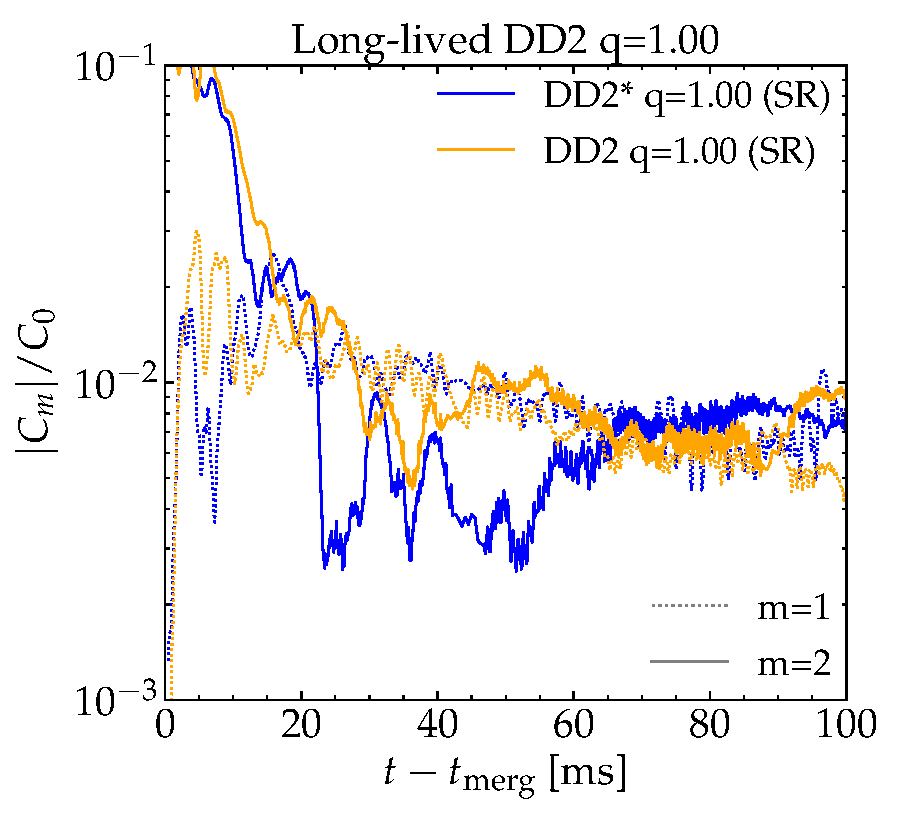
\includegraphics[width=0.49\textwidth]{remnant/dens_modes/modes_rho_dd2.pdf}
    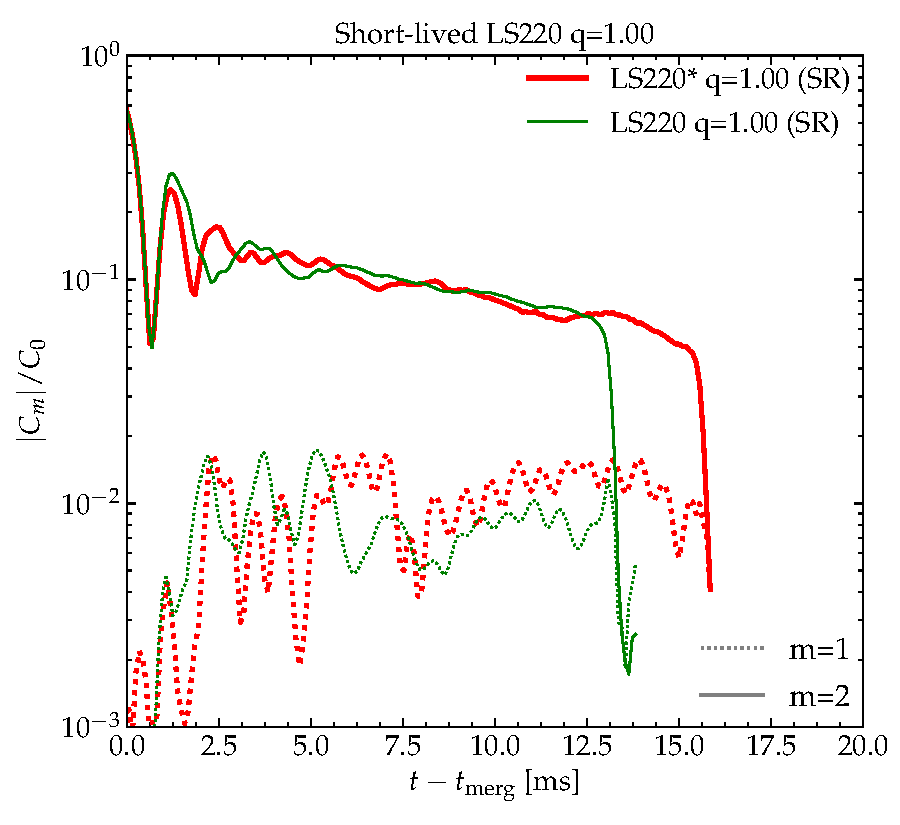
\includegraphics[width=0.49\textwidth]{remnant/dens_modes/modes_rho_ls220.pdf}
    \caption{
        The evolution of $m=1$ and $m=2$ modes in two representative 
        equal mass simulations with DD2 and LS220 \acp{EOS} on the 
        \textit{left panel} and the \textit{right panel} respectively. 
        %
        The mode amplitudes are computed via Eq.~\eqref{eq:modes}. 
        %
        The plot shows that in the case of a long-lived remnant, 
        the $m=2$ mode is dumped, \ie, decays quickly after the merger, 
        and on a timescale of ${\gtrsim}20\,$ms it becomes comaprable to 
        $m=1$ mode. 
        %
        In case of a short-lived remnant, $m=2$ remains the dominant mode 
        until the remnant collapses to a \ac{BH}.
        (Adopted from \cite{Nedora:2020pak}).
%        Modes analysis for exemplary equal-mass long-live and short-lived
%        remnants. The evolution of the $m=2$ and the $m=1$ monitored by
%        Eq.~\eqref{eq:modes} is shown for the DD2 and LS220 remnant with and
%        without turbulent viscosity. The $m=2$ mode in the long-lived
%        remnant is strongly damped by the emission of gravitational
%        radiation and becomes comparable to the $m=1$ mode on a timescale of
%        ${\gtrsim}20\,$ms. Turbulent viscosity sustain the $m=2$ mode for
%        a longer period. The $m=2$ mode is instead dominant to collapse in
%        the short-lived remnant.
%        (Adopted from \cite{Nedora:2020pak}).
    }
    \label{fig:dens_modes}
\end{figure*}


%\section{Results}


%\red{
%    To be defined: \\
%    Chirp pass \\
%    Gravitational and Baryonic masses
%}

%In this chapter we review the findings of \citet{Nedora:2019jhl} and \citet{Nedora:2020pak}
%and investigate the long-term \pmerg{} evolution of the binary neutron star. 
%
%Such studies are of high astrophysical importance as the ejecta of matter that occur 
%on various timescales \pmerg{} undergoes \rproc{} and produces observable EM emission. 
%The discussion of the \rproc{} and EM transits themselves, we resort for the chapter \red{chap:coutnerparts}.

In this chapter we present the results of the postprocessing of our 
\ac{BNS} merger simulations. 
%For the discussion on simulation methods and postprocessing techniques, 
%see Chapter \ref{ch:nr_methods}. 
%
We begin by discussing the dynamics of  \pmerg{} remnants and 
their  interactions with the surrounding disks in Sec.~\ref{sec:bns_sims:remdisk}. 
We focus on the disk evolution and its final state. Additionally, we 
assess possible evolution trajectories beyond what was simulated. 
%
Next, in Sec.~\ref{sec:bns_sims:ejecta} we analyze the properties of 
ejecta. 
Regarding \ac{DE} we focus on statistics, connecting ejecta properties to the 
binary parameters. We also take a closer look at the fast tail of \ac{DE}. 
Regarding \pmerg{} winds, we discuss the mechanism behind these winds and 
their properties.
%Additionally, we investigate the origin and properties of the fast tail of 
%\ac{DE} and \pmerg{} winds, connecting the latter to the remnant properties. 

The results presented in this and subsequent Chapters are published in 
\citet{Nedora:2019jhl,Nedora:2020pak,Nedora:2020qtd,Nedora:2021eoj,Bernuzzi:2020txg}.


%% <<<< moved from EJECTA >>>> 



%\section{Simulations}\label{sec:bns_merg:sims}
%\subsection{Simulations}

%%% --------------------------------
%%% TAB SIM SUMMARY
%%\begin{table*}
\begin{sidewaystable}
\begin{center}
\captionsetup{width=1.0\linewidth}
    \caption{
      Summary table of all the simulations and dynamical ejecta properties. The columns contain
      the following information, starting from the left. Equation of
      state, mass-ratio, available resolutions,
      inclusion of subgrid turbulence, time of the
      simulation end, time of the BH formation for LR, SR, HR
      resolutions separately, time of last output, time the disk mass
      is extracted, disk mass, mass of the
      dynamical ejecta, mass-averaged electron fracton, terminal
      velocity and RMS angle (from the binary plane) for dynamical ejecta. For all
      data except $t_{BH}$, $t_{\text{end}}$ and $t_{\text{disk}}$, the value that is given is a mean value across resolutions, with an error estimated as one
      standard diviaion from the mean. In case where only one
      resolution is present, the error is assumed to be $20\%$ of the
      value. Adopted from \citet{Nedora:2020pak}.
    }
      %% \newtxt{For discussions on errors and convergence see \citep{Radice:2018pdn,Bernuzzi:2020txg}.
      %% The model data are available online at \citep{vsevolod_nedora_2020_4159619}.
%%       }
\scalebox{0.70}{
\begin{tabular}{c c c c c c c c c c c c c}
    \hline\hline
    EOS & $q$ & $\tilde{\Lambda}$ & Resolution & GRLES & $t_{\text{end}}$ & $t_{\text{BH}}$ & $t_{\text{disk}}$ & $M_{\text{disk}} ^{\text{last}}$ & $\md$ & $\langle \yd \rangle$ & $\langle \vd  \rangle$ & $\langle \theta_{\text{ej}} ^{\text{d}} \rangle$ \\
    &   &   &  &  & [ms] & [ms] & [ms] &   & $[10^{-2} M_{\odot}]$ &   & $[c]$ &   \\ 
    \hline
    \hline
    BLh & 1.00 & 541 & \texttt{LR SR HR} & \cmark & $43.3$ $91.8$ $23.1$ & $>43.3$ $>91.8$ $>23.1$ & 23.1 & $0.166^{+0.052} _{-0.052} $ & $0.14^{+0.02} _{-0.02} $ & $0.27^{+0.01} _{-0.01} $ & $0.17^{+0.01} _{-0.01} $ & $39.65^{+0.35} _{-0.35} $ \\
    BLh & 1.00 & 541 & \texttt{LR SR} & \xmark & $15.9$ $103.2$ $ $ & $>15.9$ $>103.2$ $ $ & 15.6 & $0.261^{+0.008} _{-0.008} $ & $0.12^{+0.01} _{-0.01} $ & $0.27^{+0.01} _{-0.01} $ & $0.16^{+0.01} _{-0.01} $ & $38.80^{+0.44} _{-0.44} $ \\
%%  BLh & 1.00 & 541 & \texttt{LR SR} & \xmark & $36.9$ $15.5$ $ $ & $>36.9$ $>15.5$ $ $ & 36.6 & $0.182^{+0.091} _{-0.091} $ & $0.21^{+0.04} _{-0.04} $ & $0.26^{+0.01} _{-0.01} $ & $0.18^{+0.01} _{-0.01} $ & $36.29^{+0.24} _{-0.24} $ \\
    \hline
    BLh & 1.18 & 539 & \texttt{LR} & \cmark & $69.4$ $ $ $ $ & $>69.4$ $ $ $ $ & 69.0 & $0.202^{+0.101} _{-0.101} $ & $0.30^{+0.06} _{-0.06} $ & $0.18^{+0.04} _{-0.04} $ & $0.19^{+0.04} _{-0.04} $ & $33.65^{+6.73} _{-6.73} $ \\
    BLh & 1.18 & 539 & \texttt{LR} & \xmark & $16.4$ $ $ $ $ & $>16.4$ $ $ $ $ & 15.9 & $0.229^{+0.115} _{-0.115} $ & $0.25^{+0.05} _{-0.05} $ & $0.16^{+0.03} _{-0.03} $ & $0.20^{+0.04} _{-0.04} $ & $30.86^{+6.17} _{-6.17} $ \\
    \hline
    BLh & 1.34 & 539 & \texttt{LR SR} & \cmark & $63.4$ $9.8$ $ $ & $>63.4$ $>9.8$ $ $ & 9.8 & $0.192^{+0.004} _{-0.004} $ & $0.25^{+0.05} _{-0.05} $ & $0.14^{+0.04} _{-0.04} $ & $0.17^{+0.00} _{-0.00} $ & $28.79^{+5.00} _{-5.00} $ \\
    BLh & 1.34 & 539 & \texttt{LR} & \xmark & $18.0$ $ $ $ $ & $>18.0$ $ $ $ $ & 18.0 & $0.211^{+0.106} _{-0.106} $ & $0.19^{+0.04} _{-0.04} $ & $0.17^{+0.03} _{-0.03} $ & $0.17^{+0.03} _{-0.03} $ & $33.39^{+6.68} _{-6.68} $ \\
    \hline
    BLh & 1.43 & 540 & \texttt{LR SR} & \cmark & $35.1$ $59.6$ $ $ & $>35.1$ $>59.6$ $ $ & 33.8 & $0.265^{+0.001} _{-0.001} $ & $0.27^{+0.08} _{-0.08} $ & $0.19^{+0.03} _{-0.03} $ & $0.16^{+0.00} _{-0.00} $ & $34.49^{+3.59} _{-3.59} $ \\
    \hline
    BLh & 1.54 & 543 & \texttt{LR} & \cmark & $45.8$ $ $ $ $ & $>45.8$ $ $ $ $ & 53.8 & $0.324^{+0.162} _{-0.162} $ & $0.20^{+0.04} _{-0.04} $ & $0.17^{+0.03} _{-0.03} $ & $0.13^{+0.03} _{-0.03} $ & $31.21^{+6.24} _{-6.24} $ \\
    BLh & 1.54 & 543 & \texttt{LR} & \xmark & $17.4$ $ $ $ $ & $>17.4$ $ $ $ $ & 30.1 & $0.287^{+0.144} _{-0.144} $ & $0.22^{+0.04} _{-0.04} $ & $0.21^{+0.04} _{-0.04} $ & $0.16^{+0.03} _{-0.03} $ & $35.05^{+7.01} _{-7.01} $ \\
    \hline
    BLh & 1.66 & 538 & \texttt{LR SR} & \cmark & $64.6$ $20.1$ $ $ & $>64.6$ $1.8$ $ $ & 19.2 & $0.289^{+0.005} _{-0.005} $ & $0.42^{+0.05} _{-0.05} $ & $0.11^{+0.01} _{-0.01} $ & $0.12^{+0.01} _{-0.01} $ & $24.08^{+0.29} _{-0.29} $ \\
    \hline
    BLh & 1.82 & 532 & \texttt{LR SR HR} & \cmark & $12.0$ $17.5$ $9.6$ & $1.4$ $1.4$ $1.5$ & 5.9 & $0.170^{+0.001} _{-0.001} $ & $0.81^{+0.04} _{-0.04} $ & $0.03^{+0.01} _{-0.01} $ & $0.11^{+0.00} _{-0.00} $ & $6.53^{+0.65} _{-0.65} $ \\
    BLh & 1.82 & 532 & \texttt{LR SR HR} & \xmark & $53.8$ $26.3$ $45.2$ & $1.7$ $1.3$ $1.0$ & 43.2 & $0.098^{+0.049} _{-0.049} $ & $1.07^{+0.07} _{-0.07} $ & $0.03^{+0.01} _{-0.01} $ & $0.12^{+0.00} _{-0.00} $ & $6.27^{+0.53} _{-0.53} $ \\
    \hline
    \hline
    DD2 & 1.00 & 853 & \texttt{LR SR}    & \xmark & $92.0$ $110.2$       & $>92.0$ $>110.2$        & 9.4 & $0.154^{+0.052} _{-0.052} $ & $0.11^{+0.01} _{-0.01} $ & $0.25^{+0.00} _{-0.00} $ & $0.18^{+0.01} _{-0.01} $ & $38.07^{+0.52} _{-0.52} $ \\
    DD2 & 1.00 & 853 & \texttt{LR SR HR} & \cmark & $123.0$ $113.0$ $74.4$ & $>123.0$ $>113.0$ $>74.4$ & 8.2 & $0.111^{+0.040} _{-0.040} $ & $0.12^{+0.03} _{-0.03} $ & $0.27^{+0.01} _{-0.01} $ & $0.16^{+0.00} _{-0.00} $ & $40.03^{+0.71} _{-0.71} $ \\
    \hline
    DD2 & 1.20 & 847 & \texttt{LR SR HR} & \xmark & $37.3$ $91.0$ $55.2$ & $>37.3$ $>91.0$ $>55.2$ & 36.6 & $0.261^{+0.028} _{-0.028} $ & $0.21^{+0.08} _{-0.08} $ & $0.18^{+0.03} _{-0.03} $ & $0.17^{+0.01} _{-0.01} $ & $29.07^{+3.75} _{-3.75} $ \\
    DD2 & 1.22 & 847 & \texttt{LR SR HR} & \cmark & $42.7$ $107.3$ $19.8$ & $>42.7$ $>107.3$ $>19.8$ & 8.7 & $0.209^{+0.033} _{-0.033} $ & $0.25^{+0.02} _{-0.02} $ & $0.19^{+0.01} _{-0.01} $ & $0.17^{+0.01} _{-0.01} $ & $30.74^{+0.89} _{-0.89} $ \\
    \hline
    DD2 & 1.43 & 820 & \texttt{LR SR} & \cmark & $37.7$ $62.0$ $ $ & $>37.7$ $>62.0$ $ $ & 36.7 & $0.304^{+0.051} _{-0.051} $ & $0.70^{+0.64} _{-0.64} $ & $0.14^{+0.05} _{-0.05} $ & $0.14^{+0.01} _{-0.01} $ & $25.51^{+9.58} _{-9.58} $ \\
    \hline
    \hline
    LS220 & 1.00 & 715 & \texttt{LR SR} & \cmark & $27.0$ $27.1$ $ $ & $13.7$ $13.7$ $ $ & 16.1 & $0.073^{+0.032} _{-0.032} $ & $0.16^{+0.02} _{-0.02} $ & $0.25^{+0.02} _{-0.02} $ & $0.16^{+0.01} _{-0.01} $ & $35.70^{+0.78} _{-0.78} $ \\
    LS220 & 1.00 & 715 & \texttt{LR SR HR} & \xmark & $35.9$ $37.2$ $27.1$ & $33.4$ $16.1$ $15.4$ & 34.6 & $0.072^{+0.006} _{-0.006} $ & $0.16^{+0.06} _{-0.06} $ & $0.22^{+0.00} _{-0.00} $ & $0.16^{+0.01} _{-0.01} $ & $34.99^{+1.68} _{-1.68} $ \\
    \hline
    LS220 & 1.05 & 715 & \texttt{SR HR} & \xmark & $ $ $23.3$ $24.1$ & $ $ $17.3$ $13.9$ & 22.3 & $0.107^{+0.054} _{-0.054} $ & $0.16^{+0.02} _{-0.02} $ & $0.21^{+0.01} _{-0.01} $ & $0.16^{+0.01} _{-0.01} $ & $33.28^{+2.37} _{-2.37} $ \\
    LS220 & 1.11 & 717 & \texttt{SR HR} & \xmark & $ $ $25.1$ $24.4$ & $ $ $17.0$ $>24.4$ & 24.2 & $0.140^{+0.071} _{-0.071} $ & $0.22^{+0.03} _{-0.03} $ & $0.19^{+0.02} _{-0.02} $ & $0.18^{+0.02} _{-0.02} $ & $30.25^{+4.43} _{-4.43} $ \\
    \hline
    LS220 & 1.16 & 714 & \texttt{SR HR} & \cmark & $ $ $95.8$ $11.3$ & $ $ $68.9$ $>11.3$ & 95.5 & $0.306^{+0.153} _{-0.153} $ & $0.34^{+0.00} _{-0.00} $ & $0.22^{+0.00} _{-0.00} $ & $0.16^{+0.00} _{-0.00} $ & $34.08^{+1.00} _{-1.00} $ \\
    LS220 & 1.16 & 714 & \texttt{LR SR HR} & \xmark & $29.5$ $36.1$ $28.8$ & $>29.5$ $>36.1$ $24.1$ & - & - & $0.33^{+0.05} _{-0.05} $ & $0.17^{+0.01} _{-0.01} $ & $0.17^{+0.01} _{-0.01} $ & $30.01^{+0.64} _{-0.64} $ \\
    \hline
    LS220 & 1.43 & 710 & \texttt{LR SR} & \cmark & $19.8$ $28.5$ $ $ & $15.7$ $12.3$ $ $ & 19.6 & $0.178^{+0.072} _{-0.072} $ & $0.73^{+0.03} _{-0.03} $ & $0.16^{+0.02} _{-0.02} $ & $0.17^{+0.01} _{-0.01} $ & $26.77^{+3.50} _{-3.50} $ \\
    \hline
    LS220 & 1.66 & 707 & \texttt{LR SR} & \cmark & $6.8$ $8.0$ $ $ & $1.4$ $2.1$ $ $ & 2.0 & $0.068^{+0.008} _{-0.008} $ & $1.11^{+0.38} _{-0.38} $ & $0.07^{+0.01} _{-0.01} $ & $0.14^{+0.01} _{-0.01} $ & $13.18^{+1.33} _{-1.33} $ \\
    \hline
    \hline
    SFHo & 1.00 & 413 & \texttt{SR HR} & \cmark & $ $ $25.3$ $11.6$ & $ $ $6.0$ $4.0$ & 50.0 & $0.023^{+0.012} _{-0.012} $ & $0.40^{+0.07} _{-0.07} $ & $0.21^{+0.00} _{-0.00} $ & $0.19^{+0.01} _{-0.01} $ & $32.48^{+1.79} _{-1.79} $ \\
    SFHo & 1.00 & 413 & \texttt{LR SR HR} & \xmark & $3.2$ $7.7$ $9.0$ & $>3.2$ $4.1$ $3.8$ & 7.2 & $0.019^{+0.007} _{-0.007} $ & $0.28^{+0.07} _{-0.07} $ & $0.23^{+0.01} _{-0.01} $ & $0.21^{+0.01} _{-0.01} $ & $31.66^{+1.80} _{-1.80} $ \\
    \hline
    SFHo & 1.13 & 412 & \texttt{SR HR} & \cmark & $ $ $14.2$ $14.3$ & $ $ $6.3$ $>14.3$ & - & - & $0.44^{+0.12} _{-0.12} $ & $0.18^{+0.01} _{-0.01} $ & $0.23^{+0.01} _{-0.01} $ & $33.20^{+0.78} _{-0.78} $ \\
    SFHo & 1.13 & 412 & \texttt{LR SR HR} & \xmark & $16.5$ $19.3$ $15.2$ & $5.5$ $11.6$ $3.9$ & 15.1 & $0.046^{+0.041} _{-0.041} $ & $0.42^{+0.03} _{-0.03} $ & $0.17^{+0.03} _{-0.03} $ & $0.22^{+0.01} _{-0.01} $ & $29.63^{+4.39} _{-4.39} $ \\
    \hline
    SFHo & 1.43 & 414 & \texttt{LR} & \cmark & $19.6$ $ $ $ $ & $4.8$ $ $ $ $ & 18.9 & $0.201^{+0.101} _{-0.101} $ & $0.38^{+0.08} _{-0.08} $ & $0.14^{+0.03} _{-0.03} $ & $0.20^{+0.04} _{-0.04} $ & $29.20^{+5.84} _{-5.84} $ \\
    SFHo & 1.43 & 414 & \texttt{SR} & \cmark & $ $ $46.5$ $ $ & $ $ $>46.5$ $ $ & 50.8 & $0.241^{+0.121} _{-0.121} $ & $0.24^{+0.05} _{-0.05} $ & $0.19^{+0.04} _{-0.04} $ & $0.14^{+0.03} _{-0.03} $ & $32.86^{+6.57} _{-6.57} $ \\
    \hline
    SFHo & 1.66 & 408 & \texttt{LR SR} & \cmark & $11.2$ $16.8$ $ $ & $1.3$ $1.3$ $ $ & 11.6 & $0.177^{+0.153} _{-0.153} $ & $0.15^{+0.00} _{-0.00} $ & $0.07^{+0.00} _{-0.00} $ & $0.12^{+0.01} _{-0.01} $ & $10.39^{+1.14} _{-1.14} $ \\
    \hline
    \hline
    SLy4 & 1.00 & 402 & \texttt{LR SR} & \cmark & $10.5$ $13.1$ $ $ & $2.8$ $2.8$ $ $ & - & - & $0.09^{+0.02} _{-0.02} $ & $0.23^{+0.02} _{-0.02} $ & $0.27^{+0.02} _{-0.02} $ & $30.81^{+2.81} _{-2.81} $ \\
    SLy4 & 1.00 & 402 & \texttt{LR SR} & \xmark & $12.7$ $22.0$ $ $ & $2.7$ $13.8$ $ $ & 12.5 & $0.071^{+0.175} _{-0.175} $ & $0.31^{+0.20} _{-0.20} $ & $0.23^{+0.03} _{-0.03} $ & $0.22^{+0.01} _{-0.01} $ & $32.23^{+4.84} _{-4.84} $ \\
    \hline
    SLy4 & 1.13 & 402 & \texttt{LR SR} & \xmark & $8.4$ $20.3$ $ $ & $>8.4$ $13.0$ $ $ & 8.0 & $0.164^{+0.023} _{-0.023} $ & $0.59^{+0.07} _{-0.07} $ & $0.16^{+0.00} _{-0.00} $ & $0.24^{+0.01} _{-0.01} $ & $29.67^{+1.97} _{-1.97} $ \\
    \hline
    SLy4 & 1.43 & 399 & \texttt{SR} & \cmark & $ $ $40.3$ $ $ & $ $ $>40.3$ $ $ & 45.2 & $0.200^{+0.100} _{-0.100} $ & $0.20^{+0.04} _{-0.04} $ & $0.21^{+0.04} _{-0.04} $ & $0.15^{+0.03} _{-0.03} $ & $34.03^{+6.81} _{-6.81} $ \\
    \hline
    SLy4 & 1.66 & 397 & \texttt{SR} & \cmark & $ $ $7.2$ $ $ & $ $ $1.2$ $ $ & 3.9 & $0.138^{+0.069} _{-0.069} $ & $0.28^{+0.06} _{-0.06} $ & $0.05^{+0.01} _{-0.01} $ & $0.12^{+0.02} _{-0.02} $ & $8.43^{+1.69} _{-1.69} $ \\
    \hline\hline
\end{tabular}
\label{tab:sim}
}%scalebox
\end{center}
%\end{table*}
\end{sidewaystable}



%\usepackage{lipsum}% dummy text
%\begin{document}
    %\lipsum % Text before
%    \afterpage{%
%        \clearpage% Flush earlier floats (otherwise order might not be correct)
%        \thispagestyle{empty}% empty page style (?)
%        \begin{landscape}% Landscape page
%            \centering % Center table
%            \begin{tabular}{c c c c c c c c c c c c c}
%                \hline\hline
%                EOS & $q$ & $\tilde{\Lambda}$ & Resolution & GRLES & $t_{\text{end}}$ & $t_{\text{BH}}$ & $t_{\text{disk}}$ & $M_{\text{disk}} ^{\text{last}}$ & $\md$ & $\langle \yd \rangle$ & $\langle \vd  \rangle$ & $\langle \theta_{\text{ej}} ^{\text{d}} \rangle$ \\
%                &   &   &  &  & [ms] & [ms] & [ms] &   & $[10^{-2} M_{\odot}]$ &   & $[c]$ &   \\ 
%                \hline
%                \hline
%                BLh & 1.00 & 541 & \texttt{LR SR HR} & \cmark & $43.3$ $91.8$ $23.1$ & $>43.3$ $>91.8$ $>23.1$ & 23.1 & $0.166^{+0.052} _{-0.052} $ & $0.14^{+0.02} _{-0.02} $ & $0.27^{+0.01} _{-0.01} $ & $0.17^{+0.01} _{-0.01} $ & $39.65^{+0.35} _{-0.35} $ \\
%                BLh & 1.00 & 541 & \texttt{LR SR} & \xmark & $15.9$ $103.2$ $ $ & $>15.9$ $>103.2$ $ $ & 15.6 & $0.261^{+0.008} _{-0.008} $ & $0.12^{+0.01} _{-0.01} $ & $0.27^{+0.01} _{-0.01} $ & $0.16^{+0.01} _{-0.01} $ & $38.80^{+0.44} _{-0.44} $ \\
%                %%  BLh & 1.00 & 541 & \texttt{LR SR} & \xmark & $36.9$ $15.5$ $ $ & $>36.9$ $>15.5$ $ $ & 36.6 & $0.182^{+0.091} _{-0.091} $ & $0.21^{+0.04} _{-0.04} $ & $0.26^{+0.01} _{-0.01} $ & $0.18^{+0.01} _{-0.01} $ & $36.29^{+0.24} _{-0.24} $ \\
%                \hline
%                BLh & 1.18 & 539 & \texttt{LR} & \cmark & $69.4$ $ $ $ $ & $>69.4$ $ $ $ $ & 69.0 & $0.202^{+0.101} _{-0.101} $ & $0.30^{+0.06} _{-0.06} $ & $0.18^{+0.04} _{-0.04} $ & $0.19^{+0.04} _{-0.04} $ & $33.65^{+6.73} _{-6.73} $ \\
%                BLh & 1.18 & 539 & \texttt{LR} & \xmark & $16.4$ $ $ $ $ & $>16.4$ $ $ $ $ & 15.9 & $0.229^{+0.115} _{-0.115} $ & $0.25^{+0.05} _{-0.05} $ & $0.16^{+0.03} _{-0.03} $ & $0.20^{+0.04} _{-0.04} $ & $30.86^{+6.17} _{-6.17} $ \\
%                \hline
%                BLh & 1.34 & 539 & \texttt{LR SR} & \cmark & $63.4$ $9.8$ $ $ & $>63.4$ $>9.8$ $ $ & 9.8 & $0.192^{+0.004} _{-0.004} $ & $0.25^{+0.05} _{-0.05} $ & $0.14^{+0.04} _{-0.04} $ & $0.17^{+0.00} _{-0.00} $ & $28.79^{+5.00} _{-5.00} $ \\
%                BLh & 1.34 & 539 & \texttt{LR} & \xmark & $18.0$ $ $ $ $ & $>18.0$ $ $ $ $ & 18.0 & $0.211^{+0.106} _{-0.106} $ & $0.19^{+0.04} _{-0.04} $ & $0.17^{+0.03} _{-0.03} $ & $0.17^{+0.03} _{-0.03} $ & $33.39^{+6.68} _{-6.68} $ \\
%                \hline
%                BLh & 1.43 & 540 & \texttt{LR SR} & \cmark & $35.1$ $59.6$ $ $ & $>35.1$ $>59.6$ $ $ & 33.8 & $0.265^{+0.001} _{-0.001} $ & $0.27^{+0.08} _{-0.08} $ & $0.19^{+0.03} _{-0.03} $ & $0.16^{+0.00} _{-0.00} $ & $34.49^{+3.59} _{-3.59} $ \\
%                \hline
%                BLh & 1.54 & 543 & \texttt{LR} & \cmark & $45.8$ $ $ $ $ & $>45.8$ $ $ $ $ & 53.8 & $0.324^{+0.162} _{-0.162} $ & $0.20^{+0.04} _{-0.04} $ & $0.17^{+0.03} _{-0.03} $ & $0.13^{+0.03} _{-0.03} $ & $31.21^{+6.24} _{-6.24} $ \\
%                BLh & 1.54 & 543 & \texttt{LR} & \xmark & $17.4$ $ $ $ $ & $>17.4$ $ $ $ $ & 30.1 & $0.287^{+0.144} _{-0.144} $ & $0.22^{+0.04} _{-0.04} $ & $0.21^{+0.04} _{-0.04} $ & $0.16^{+0.03} _{-0.03} $ & $35.05^{+7.01} _{-7.01} $ \\
%                \hline
%                BLh & 1.66 & 538 & \texttt{LR SR} & \cmark & $64.6$ $20.1$ $ $ & $>64.6$ $1.8$ $ $ & 19.2 & $0.289^{+0.005} _{-0.005} $ & $0.42^{+0.05} _{-0.05} $ & $0.11^{+0.01} _{-0.01} $ & $0.12^{+0.01} _{-0.01} $ & $24.08^{+0.29} _{-0.29} $ \\
%                \hline
%                BLh & 1.82 & 532 & \texttt{LR SR HR} & \cmark & $12.0$ $17.5$ $9.6$ & $1.4$ $1.4$ $1.5$ & 5.9 & $0.170^{+0.001} _{-0.001} $ & $0.81^{+0.04} _{-0.04} $ & $0.03^{+0.01} _{-0.01} $ & $0.11^{+0.00} _{-0.00} $ & $6.53^{+0.65} _{-0.65} $ \\
%                BLh & 1.82 & 532 & \texttt{LR SR HR} & \xmark & $53.8$ $26.3$ $45.2$ & $1.7$ $1.3$ $1.0$ & 43.2 & $0.098^{+0.049} _{-0.049} $ & $1.07^{+0.07} _{-0.07} $ & $0.03^{+0.01} _{-0.01} $ & $0.12^{+0.00} _{-0.00} $ & $6.27^{+0.53} _{-0.53} $ \\
%                \hline
%                \hline
%                DD2 & 1.00 & 853 & \texttt{LR SR}    & \xmark & $92.0$ $110.2$       & $>92.0$ $>110.2$        & 9.4 & $0.154^{+0.052} _{-0.052} $ & $0.11^{+0.01} _{-0.01} $ & $0.25^{+0.00} _{-0.00} $ & $0.18^{+0.01} _{-0.01} $ & $38.07^{+0.52} _{-0.52} $ \\
%                DD2 & 1.00 & 853 & \texttt{LR SR HR} & \cmark & $123.0$ $113.0$ $74.4$ & $>123.0$ $>113.0$ $>74.4$ & 8.2 & $0.111^{+0.040} _{-0.040} $ & $0.12^{+0.03} _{-0.03} $ & $0.27^{+0.01} _{-0.01} $ & $0.16^{+0.00} _{-0.00} $ & $40.03^{+0.71} _{-0.71} $ \\
%                \hline
%                DD2 & 1.20 & 847 & \texttt{LR SR HR} & \xmark & $37.3$ $91.0$ $55.2$ & $>37.3$ $>91.0$ $>55.2$ & 36.6 & $0.261^{+0.028} _{-0.028} $ & $0.21^{+0.08} _{-0.08} $ & $0.18^{+0.03} _{-0.03} $ & $0.17^{+0.01} _{-0.01} $ & $29.07^{+3.75} _{-3.75} $ \\
%                DD2 & 1.22 & 847 & \texttt{LR SR HR} & \cmark & $42.7$ $107.3$ $19.8$ & $>42.7$ $>107.3$ $>19.8$ & 8.7 & $0.209^{+0.033} _{-0.033} $ & $0.25^{+0.02} _{-0.02} $ & $0.19^{+0.01} _{-0.01} $ & $0.17^{+0.01} _{-0.01} $ & $30.74^{+0.89} _{-0.89} $ \\
%                \hline
%                DD2 & 1.43 & 820 & \texttt{LR SR} & \cmark & $37.7$ $62.0$ $ $ & $>37.7$ $>62.0$ $ $ & 36.7 & $0.304^{+0.051} _{-0.051} $ & $0.70^{+0.64} _{-0.64} $ & $0.14^{+0.05} _{-0.05} $ & $0.14^{+0.01} _{-0.01} $ & $25.51^{+9.58} _{-9.58} $ \\
%                \hline
%                \hline
%                LS220 & 1.00 & 715 & \texttt{LR SR} & \cmark & $27.0$ $27.1$ $ $ & $13.7$ $13.7$ $ $ & 16.1 & $0.073^{+0.032} _{-0.032} $ & $0.16^{+0.02} _{-0.02} $ & $0.25^{+0.02} _{-0.02} $ & $0.16^{+0.01} _{-0.01} $ & $35.70^{+0.78} _{-0.78} $ \\
%                LS220 & 1.00 & 715 & \texttt{LR SR HR} & \xmark & $35.9$ $37.2$ $27.1$ & $33.4$ $16.1$ $15.4$ & 34.6 & $0.072^{+0.006} _{-0.006} $ & $0.16^{+0.06} _{-0.06} $ & $0.22^{+0.00} _{-0.00} $ & $0.16^{+0.01} _{-0.01} $ & $34.99^{+1.68} _{-1.68} $ \\
%                \hline
%                LS220 & 1.05 & 715 & \texttt{SR HR} & \xmark & $ $ $23.3$ $24.1$ & $ $ $17.3$ $13.9$ & 22.3 & $0.107^{+0.054} _{-0.054} $ & $0.16^{+0.02} _{-0.02} $ & $0.21^{+0.01} _{-0.01} $ & $0.16^{+0.01} _{-0.01} $ & $33.28^{+2.37} _{-2.37} $ \\
%                LS220 & 1.11 & 717 & \texttt{SR HR} & \xmark & $ $ $25.1$ $24.4$ & $ $ $17.0$ $>24.4$ & 24.2 & $0.140^{+0.071} _{-0.071} $ & $0.22^{+0.03} _{-0.03} $ & $0.19^{+0.02} _{-0.02} $ & $0.18^{+0.02} _{-0.02} $ & $30.25^{+4.43} _{-4.43} $ \\
%                \hline
%                LS220 & 1.16 & 714 & \texttt{SR HR} & \cmark & $ $ $95.8$ $11.3$ & $ $ $68.9$ $>11.3$ & 95.5 & $0.306^{+0.153} _{-0.153} $ & $0.34^{+0.00} _{-0.00} $ & $0.22^{+0.00} _{-0.00} $ & $0.16^{+0.00} _{-0.00} $ & $34.08^{+1.00} _{-1.00} $ \\
%                LS220 & 1.16 & 714 & \texttt{LR SR HR} & \xmark & $29.5$ $36.1$ $28.8$ & $>29.5$ $>36.1$ $24.1$ & - & - & $0.33^{+0.05} _{-0.05} $ & $0.17^{+0.01} _{-0.01} $ & $0.17^{+0.01} _{-0.01} $ & $30.01^{+0.64} _{-0.64} $ \\
%                \hline
%                LS220 & 1.43 & 710 & \texttt{LR SR} & \cmark & $19.8$ $28.5$ $ $ & $15.7$ $12.3$ $ $ & 19.6 & $0.178^{+0.072} _{-0.072} $ & $0.73^{+0.03} _{-0.03} $ & $0.16^{+0.02} _{-0.02} $ & $0.17^{+0.01} _{-0.01} $ & $26.77^{+3.50} _{-3.50} $ \\
%                \hline
%                LS220 & 1.66 & 707 & \texttt{LR SR} & \cmark & $6.8$ $8.0$ $ $ & $1.4$ $2.1$ $ $ & 2.0 & $0.068^{+0.008} _{-0.008} $ & $1.11^{+0.38} _{-0.38} $ & $0.07^{+0.01} _{-0.01} $ & $0.14^{+0.01} _{-0.01} $ & $13.18^{+1.33} _{-1.33} $ \\
%                \hline
%                \hline
%                SFHo & 1.00 & 413 & \texttt{SR HR} & \cmark & $ $ $25.3$ $11.6$ & $ $ $6.0$ $4.0$ & 50.0 & $0.023^{+0.012} _{-0.012} $ & $0.40^{+0.07} _{-0.07} $ & $0.21^{+0.00} _{-0.00} $ & $0.19^{+0.01} _{-0.01} $ & $32.48^{+1.79} _{-1.79} $ \\
%                SFHo & 1.00 & 413 & \texttt{LR SR HR} & \xmark & $3.2$ $7.7$ $9.0$ & $>3.2$ $4.1$ $3.8$ & 7.2 & $0.019^{+0.007} _{-0.007} $ & $0.28^{+0.07} _{-0.07} $ & $0.23^{+0.01} _{-0.01} $ & $0.21^{+0.01} _{-0.01} $ & $31.66^{+1.80} _{-1.80} $ \\
%                \hline
%                SFHo & 1.13 & 412 & \texttt{SR HR} & \cmark & $ $ $14.2$ $14.3$ & $ $ $6.3$ $>14.3$ & - & - & $0.44^{+0.12} _{-0.12} $ & $0.18^{+0.01} _{-0.01} $ & $0.23^{+0.01} _{-0.01} $ & $33.20^{+0.78} _{-0.78} $ \\
%                SFHo & 1.13 & 412 & \texttt{LR SR HR} & \xmark & $16.5$ $19.3$ $15.2$ & $5.5$ $11.6$ $3.9$ & 15.1 & $0.046^{+0.041} _{-0.041} $ & $0.42^{+0.03} _{-0.03} $ & $0.17^{+0.03} _{-0.03} $ & $0.22^{+0.01} _{-0.01} $ & $29.63^{+4.39} _{-4.39} $ \\
%                \hline
%                SFHo & 1.43 & 414 & \texttt{LR} & \cmark & $19.6$ $ $ $ $ & $4.8$ $ $ $ $ & 18.9 & $0.201^{+0.101} _{-0.101} $ & $0.38^{+0.08} _{-0.08} $ & $0.14^{+0.03} _{-0.03} $ & $0.20^{+0.04} _{-0.04} $ & $29.20^{+5.84} _{-5.84} $ \\
%                SFHo & 1.43 & 414 & \texttt{SR} & \cmark & $ $ $46.5$ $ $ & $ $ $>46.5$ $ $ & 50.8 & $0.241^{+0.121} _{-0.121} $ & $0.24^{+0.05} _{-0.05} $ & $0.19^{+0.04} _{-0.04} $ & $0.14^{+0.03} _{-0.03} $ & $32.86^{+6.57} _{-6.57} $ \\
%                \hline
%                SFHo & 1.66 & 408 & \texttt{LR SR} & \cmark & $11.2$ $16.8$ $ $ & $1.3$ $1.3$ $ $ & 11.6 & $0.177^{+0.153} _{-0.153} $ & $0.15^{+0.00} _{-0.00} $ & $0.07^{+0.00} _{-0.00} $ & $0.12^{+0.01} _{-0.01} $ & $10.39^{+1.14} _{-1.14} $ \\
%                \hline
%                \hline
%                SLy4 & 1.00 & 402 & \texttt{LR SR} & \cmark & $10.5$ $13.1$ $ $ & $2.8$ $2.8$ $ $ & - & - & $0.09^{+0.02} _{-0.02} $ & $0.23^{+0.02} _{-0.02} $ & $0.27^{+0.02} _{-0.02} $ & $30.81^{+2.81} _{-2.81} $ \\
%                SLy4 & 1.00 & 402 & \texttt{LR SR} & \xmark & $12.7$ $22.0$ $ $ & $2.7$ $13.8$ $ $ & 12.5 & $0.071^{+0.175} _{-0.175} $ & $0.31^{+0.20} _{-0.20} $ & $0.23^{+0.03} _{-0.03} $ & $0.22^{+0.01} _{-0.01} $ & $32.23^{+4.84} _{-4.84} $ \\
%                \hline
%                SLy4 & 1.13 & 402 & \texttt{LR SR} & \xmark & $8.4$ $20.3$ $ $ & $>8.4$ $13.0$ $ $ & 8.0 & $0.164^{+0.023} _{-0.023} $ & $0.59^{+0.07} _{-0.07} $ & $0.16^{+0.00} _{-0.00} $ & $0.24^{+0.01} _{-0.01} $ & $29.67^{+1.97} _{-1.97} $ \\
%                \hline
%                SLy4 & 1.43 & 399 & \texttt{SR} & \cmark & $ $ $40.3$ $ $ & $ $ $>40.3$ $ $ & 45.2 & $0.200^{+0.100} _{-0.100} $ & $0.20^{+0.04} _{-0.04} $ & $0.21^{+0.04} _{-0.04} $ & $0.15^{+0.03} _{-0.03} $ & $34.03^{+6.81} _{-6.81} $ \\
%                \hline
%                SLy4 & 1.66 & 397 & \texttt{SR} & \cmark & $ $ $7.2$ $ $ & $ $ $1.2$ $ $ & 3.9 & $0.138^{+0.069} _{-0.069} $ & $0.28^{+0.06} _{-0.06} $ & $0.05^{+0.01} _{-0.01} $ & $0.12^{+0.02} _{-0.02} $ & $8.43^{+1.69} _{-1.69} $ \\
%                \hline\hline
%            \end{tabular}
%            \captionof{table}{
%            Summary table of all the simulations and dynamical ejecta properties. The columns contain
%            the following information, starting from the left. Equation of
%            state, mass-ratio, available resolutions,
%            inclusion of subgrid turbulence, time of the
%            simulation end, time of the BH formation for LR, SR, HR
%            resolutions separately, time of last output, time the disk mass
%            is extracted, disk mass, mass of the
%            dynamical ejecta, mass-averaged electron fracton, terminal
%            velocity and RMS angle (from the binary plane) for dynamical ejecta. For all
%            data except $t_{BH}$, $t_{\text{end}}$ and $t_{\text{disk}}$, the value that is given is a mean value across resolutions, with an error estimated as one
%            standard diviaion from the mean. In case where only one
%            resolution is present, the error is assumed to be $20\%$ of the
%            value. Adopted from \citet{Nedora:2020pak}.
%        }% Add 'table' caption
%        \end{landscape}
%        \clearpage% Flush page
%    }
%    %\lipsum % Text after
%%\end{document}




























%%% --------------------------------
%
%
%In total we consider a sample of $37$ models of unique binaries with the 
%chirp mass $\mathcal{M}_c = 1.188\,\Msun$ that corresponds to the source of \GW{}.
%%
%The total gravitational mass covers the range $M\in[2.73, 2.88]\,\Msun$, while the 
%mas ration $q=M_A/M_B\in[1,1.8]$. 
%%
%We show the masses and radii of computed models as markers in 
%Fig.~\ref{fig:method:tov_mr} and summarize their main properties, 
%and the dynamical ejecta properties in Tab.~\ref{tab:sim}.
%%
%Most simulations are performed with at least two resolutions, 
%\texttt{LR} and \texttt{SR}. 
%$16$ binaries are also simulated at high resolution, \texttt{HR}.
%In total $76$ models are computed and analyzed.
%%
%Several binaries that resulted in a formation of a \ac{NS} remnant that does not collapse 
%to a \ac{BH} are evolved up to $100\,$ms \pmerg.
%%
%Most simulations include the effects of subgrid turbulence. 
%Those that are not are marked with ``*'' next to the equation of state name.
%%
%The naming convention for simulations is the following: 
%the equation of state name, the mass ratio, and the resolution, \eg, 
%the ``BLh* $q=1.00$ (\texttt{SR})" would refer to the simulation of the equal mass
%binary performed with BLh \ac{EOS}, without subgrid turbulence and at standard resolution. If resolution is not mentioned, \texttt{SR} is assumed.
%%\red{might be redundant}
%%% mass ratio binaries has been already presented in \cite{Bernuzzi:2020txg}.
%%% Together with our previous data these simulations form the largest
%%% sample of merger simulations with microphysics available to date
%%% \citep{Bernuzzi:2015opx,Radice:2016dwd,Radice:2016rys,Radice:2017lry,
%%%        Radice:2018xqa,Radice:2018pdn,Perego:2019adq,Endrizzi:2019trv,Bernuzzi:2020txg}.  



%% ----------------------------------------------------------------------
%%
%% O V E R V I E W  O F  T H E  M E R G E R  D Y N A M I C S
%%
%% ----------------------------------------------------------------------

%\subsection{Overview of the remnant dynamics}
%\section{Overview of the remnant dynamics}
%\label{sec:bns_dynsmics_overview}


%This section is based on the \cite{Nedora:2020pak}





%\subsection{Overview}

%A newly born \ac{NS} \pmerg{} remnant is not axisymmetric. In addition to driving the angular 
%momentum transport, it is a strong emitter of \acp{GW} at kiloHertz frequencies.
%In ${\sim}10-20\,$ms \pmerg{} \acp{GW} remove about two times the 
%amount of energy that was lost during the inspiral and merger \citep{Bernuzzi:2015opx}.
%%
%After that, the contribution of \acp{GW} to the system evolution, specifically to the 
%angular momentum loss, drops \citep{Radice:2018xqa}. The long-term evolution, $\mathcal{O}(100)\,$ms,
%of the remnant is driven primarily by viscous processes and weak interactions.
%%
%After the emission of \acp{GW} subsides, the \ac{NS} remnant still has an excess 
%in angular momentum and gravitational mass, with respect to the cold, 
%rigidly rotating equilibrium with the same baryoinc mass \citep{Radice:2018xqa}.
%%
%Subsequent evolution of the \ac{NS} remnant proceeds towards the axisymmetric configuration 
%close to the mass-shedding limit. 
%Depending on the lifetime of the \ac{NS} remnant we distinguish \textit{long-lived}
%and \textit{short-lived} remnants (See also \ref{sec:intro:remnant}).
%However, would a \ac{NS} remnant reach a stable state or collapse to a \ac{BH} depends on the 
%details of \pmerg{} conditions and on the temperature and composition effects.
%

%% -------------------------------------------------------------
%%
%% R E M N A N T  D I S K  I N T E R A C T I O N
%%
%% -------------------------------------------------------------

\section{Overview of the remnant-disk interactions}\label{sec:bns_sims:remdisk}
%\subsection{Remnant-disk interaction}\label{sec:bns_sims:remdisk}



We begin by analyzing the dynamics of \pmerg{} \ac{NS} remnants.
Hydrodynamic instabilities are monitored by a decomposition in Fourier modes,
$e^{-i m \phi}$, of the Eulerian rest-mass density on the equatorial plane 
(see Sec.~\ref{sec:bns_sims:method:modes} for more details).
%[see Eq.~(1) of \citep{Radice:2016gym}] and characterized by the
%development of a $m=2$ followed by a $m=1$ mode 
%\citep{East:2015vix,Paschalidis:2015mla,Radice:2016gym,Lehner:2016wjg,Bernuzzi:2013rza,Kastaun:2014fna}.
%
%We begin by analyzing the \pmerg{} dynamics of the \ac{NS} remnant. The standard 
%probe is employed here, namely the complex decomposition of the hydrodynamical modes
%(see Sec.~\ref{sec:bns_sims:method:modes}). 
%
We consider two representative simulations, 
LS220 $q=1.00$ (\texttt{SR}) %the model with LS220 \ac{EOS}, $q=1.00$ and a 
and 
DD2 $q=1.00$ (\texttt{SR}), 
that produce short- and long-lived remnants respectively.

%
As we mentioned in Sec.~\ref{sec:intro:merg_pmerg}, 
newly born \ac{NS} remnants are not axisymmetric, 
displaying characteristic spiral arms in their density 
profile that extend outwards from the shock interface of collided cores. 
%\citep{Shibata:1999wm,
%    Shibata:2006nm,Bernuzzi:2013rza,Kastaun:2014fna,East:2015vix,Paschalidis:2015mla,
%    Radice:2016gym,Lehner:2016wjg
%}.
%
%These arms, albet in terms of the angular momentum flux (defined in Sec.~\ref{sec:bns_sims:method:ang_mom}) can be seen in Fig.~\ref{fig:ang_mom_flux}. 
%
%Indeed, our analysis, results of which are displayed in Fig.~\ref{fig:dens_modes}, 
%shows, that 
Specifically, 
%The result of the mode analysis is shown in Fig.~\ref{fig:dens_modes}. 
the $m=2$ instability, characterized by the bar-shaped geometry, dominates 
the early \pmerg{}, while the $m=1$ instability, characterized by one-armed geometry,  
starts to dominate in the late evolution 
\citep[\eg][]{East:2015vix,Radice:2016gym, %Paschalidis:2015mla,Radice:2016gym,Lehner:2016wjg,
    Bernuzzi:2013rza,Kastaun:2014fna}.
Fig.~\ref{fig:dens_modes} corroborates this picture.
%
%\red{One sentence 'why', physically}
%
Indeed, the $m=2$ mode remains the dominant one until 
${\sim}15-20\,$ms \pmerg{}. 
After that, the 
LS220 $q=1.00$ model 
%model with LS220 \ac{EOS} and $q=1.00$
forms a \ac{BH}. 
In the 
DD2 $q=1.00$ model, 
%model with DD2 \ac{EOS} and $q=1.00$ model, 
however, the amplitude the of the $m=1$ mode 
becomes comparable with that of the $m=2$, and 
both modes persist throughout the remainder of the evolution,
after the \ac{GW}-dominated phase ends 
%while 
%the $m=2$ mode efficiently dissipates through \ac{GW} emission 
\citep{Bernuzzi:2015opx,Radice:2016gym}. 
%
%\red{Why $m=1$ does not dissipates via \acp{GW}}
%
%Notably, the inclusion of subgrid turbulence sustains $m=1$ 
%on a longer timescale.

We find that the magnitude of the $m=1$ mode increases with the binary \mr{}.
For instance, the largest $C_{m=1}$ are found in models with 
BLh and LS220 \acp{EOS} and \mr{}s $q=1.43$ and $q=1.22$ respectively. 
% Stronger $m=1$ leads to more large \ac{SWW} mass flux.  %------------------------------------------- ABOUT WIND
The dependency of the $C_{m=2}$ on \mr{}, however, is not very clear. 
Overall, our results are in agreement with what was 
reported by \citet{Lehner:2016wjg}.


\begin{figure}[t]
    \centering
    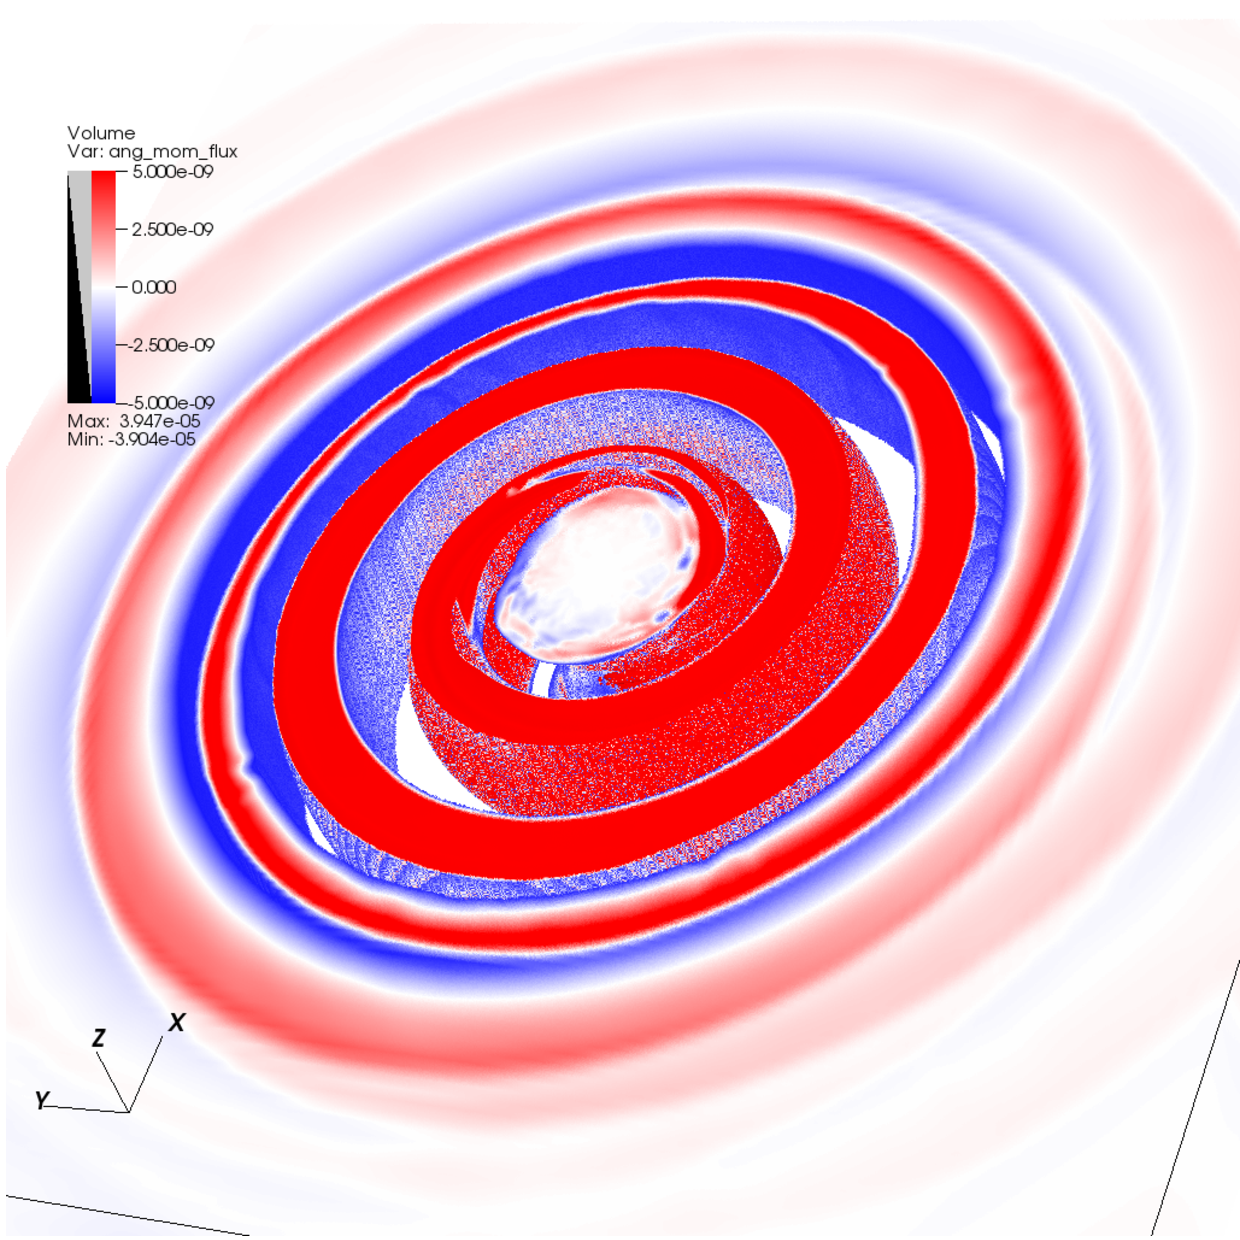
\includegraphics[width=0.49\textwidth]{raycasting_smooth_cropped.pdf}
    \caption{
        Volume rendering of the angular momentum flux, $J_r$, 
        distribution in $3D$ for DD2 $q=1.00$ \texttt{SR} model. 
        The snapshot is taken at ${\sim}43.5$~ms after
        merger. $J_r$ is shown on a central region of
        $(89\times89\times60)$~km${}^3$ covering the remnant NS
        and disk, and it is given in units where $c=G=\Msun=1$.
        (Adapted from \citet{Nedora:2019jhl}).
    }
    \label{fig:ang_mom_flux}
\end{figure}

\begin{figure}[t]
    \centering 
    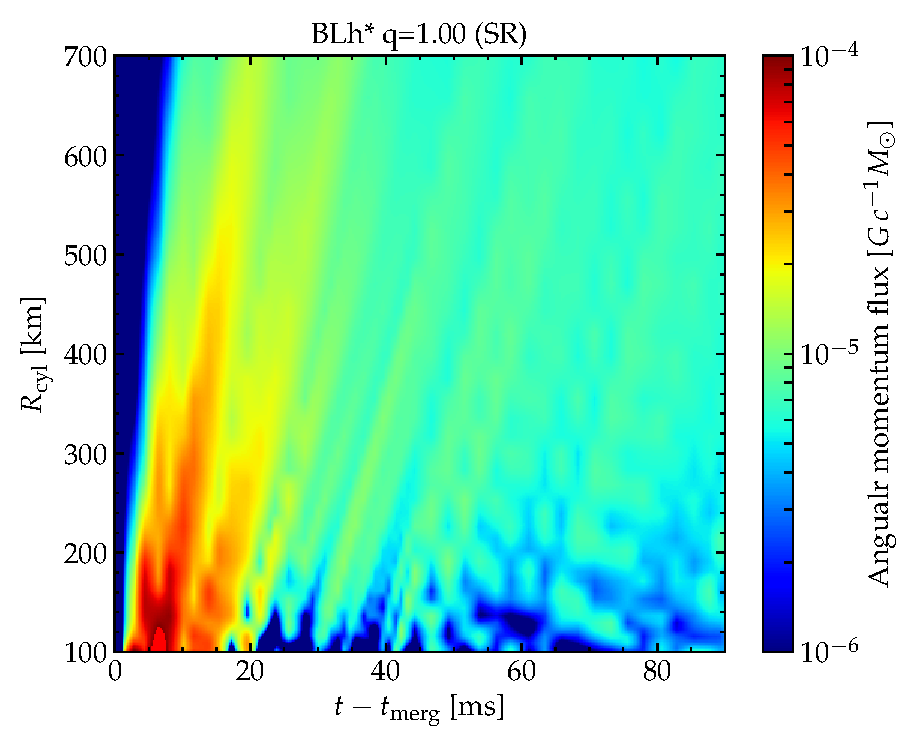
\includegraphics[width=0.49\textwidth]{remnant/evol_jflux_2d_BLh_M13651365_M0_SR_R1.pdf}
    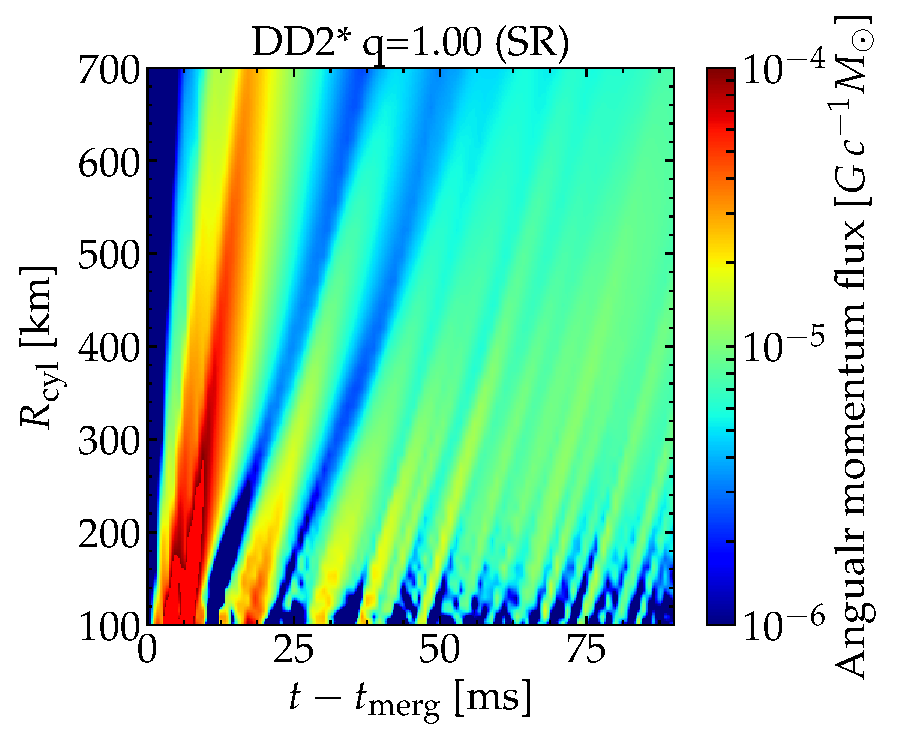
\includegraphics[width=0.49\textwidth]{remnant/evol_jflux_2d_DD2_M13641364_M0_SR_R1.pdf}
    \caption{
        The evolution of the angular momentum flux through consecutive cylindrical
        surfaces 
        (for cylindrical radii from $R_{\text{cyl}}=100$ to $R_{\text{cyl}}=500$). 
        The angular momentum transport through the disk is depicted 
        for two equal mass \ac{BNS} \pmerg{} remnants without viscosity.
        (Adapted from \citet{Nedora:2020pak}).
    }
    \label{fig:disk_ang_mom_flux_map_blh_q1}
\end{figure}


The formation of spiral arms is a generic hydrodynamic effect 
that was identified in \ac{NR} simulations with polytropic 
\acp{EOS} \citep{Bernuzzi:2013rza,Radice:2016gym}.
However, the evolution of these arms and the quantitative behaviour of hydrodynamic
modes depend on the physics input of simulations, and are not well understood. 
We observe that turbulent viscosity, for instance, 
leads to faster suppression of $m=2$. By contrast, the $m=1$ mode is not
significantly affected by viscosity, as shown in Fig.~\ref{fig:dens_modes}.
%
If a remnant is short-lived, as is the case for LS220 $q=1.00$ model, 
%with LS22 \ac{EOS} and $q=1.00$, 
the effect of subgrid turbulence is not apparent because 
the dynamical evolution is interrupted by the collapse.

%From the fluid's stress energy tensor,
%we compute the angular momentum density flux $J_r = T_{ra}(\p_\phi)^a$,
%where $\phi$ is the cylindrical angular coordinate;
%angular momentum is conserved if $(\p_\phi)^a$ is a Killing vector.
%
We compute the angular momentum and its flux from the energy-momentum 
tensor, Eq.~\eqref{eq:theory:tmunu_perf},
in cylindrical coordinates, $(r,\, \phi,\, z)$, under the additional
assumption of axisymmetry %with $(\partial_{\phi})^a$ being a Killing vector
(see Sec.~\ref{sec:bns_sims:method:ang_mom} for more details).
%
The disk is assumed to be comprised of matter with $\rho\leq10^{13}\,$\gcm{} 
(see also Sec.~\ref{sec:bns_sims:method:disk}).

We find that for a long-lived \ac{NS} remnant on a timescale of ${\sim}20$~ms, 
about half of the total angular momentum of the remnant is transferred 
into the disk. 
%% [ from shibata review ]
This is a consequence of the fact that the remnant \ac{NS} is strongly deformed 
after merger and exerts gravitational torques on the surrounding matter, 
allowing for a rapid angular momentum transport.
%% ---
%After, the remnant and the disk settle on quasi-stationary evolution path.
%(see Sec.~\ref{sec:bns_dynsmics_overview}).

Following the disk and remnant mass evolution we observe that the spiral 
density modes inject ${\sim}0.1-0.4\,\Msun$ of baryon mass into the disk during the 
first ${\sim}20\,$ms. 
The mass injection appears to be stronger in models with stiffer \acp{EOS}. 
With respect to the \mr{}, we find that higher $q$ binaries form more massive disks 
\eg, the BLh* $q=1.82$ model (that undergoes \ac{PC}) and the
LS220* $q=1.43$ model. 
%We discuss the disk masses and their evolution in more details shortly.
%shown in Fig.~\ref{fig:disk_mass_evo}.
%
%(see model with BLh \ac{EOS}, $q=1.82$ and model with LS220 \ac{EOS} $q=1.43$ 
%on the Fig.~\ref{fig:disk_mass_evo} that do not have turbulent viscosity).

\begin{figure}[t]
    \centering 
    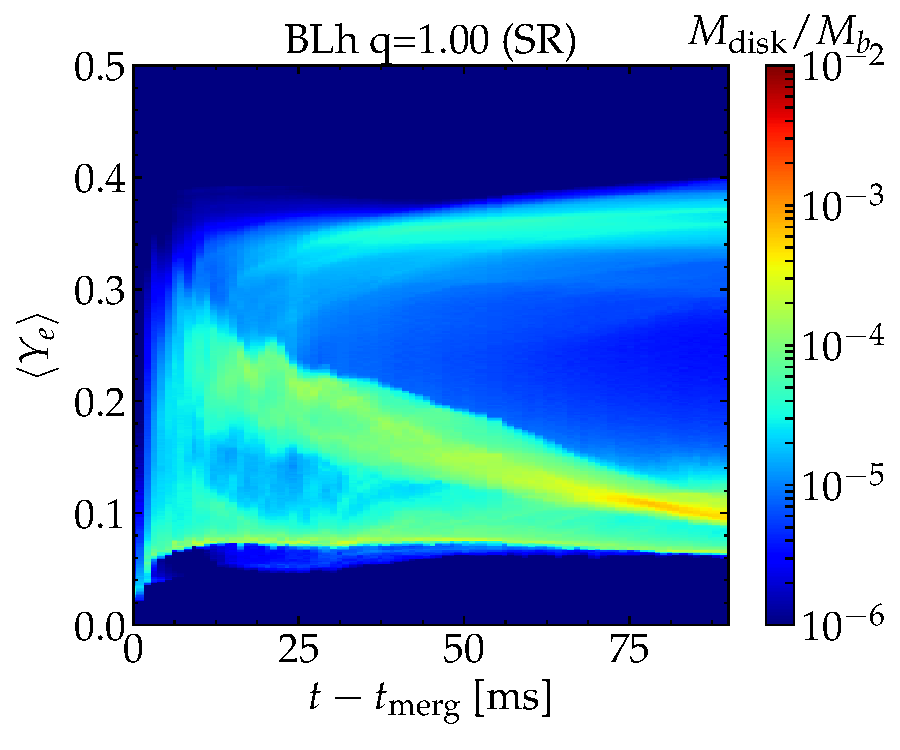
\includegraphics[width=0.49\textwidth]{disk/final_disk_timecorr_blh_q1_Lk.pdf}
    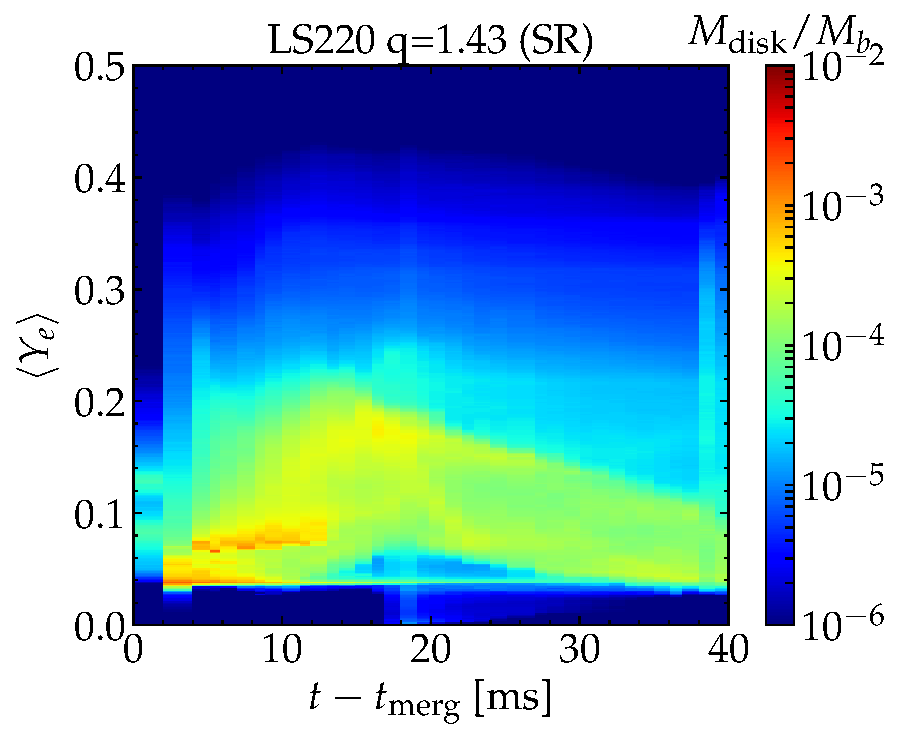
\includegraphics[width=0.49\textwidth]{disk/final_disk_timecorr_ls220_q14_LK.pdf}
    \caption{
        Evolution of the mass-averaged electron fraction in 
        the disk of two models, BLh $q=1.00$ and LS220 $q=1.43$ shown on the 
        \textit{left panel} and \textit{right panel} respectively, that produce 
        long- and short-lived remnants respectively.
        %
        The plot shows that during the \pmerg{} evolution, neutrino 
        cooling lowers the $Y_e$ of the bulk of the disk matter. 
        A small fraction of the disk, however, reaches higher $Y_e$, 
        while being irradiated by neutrinos and processed by shocks 
        %
        (Adapted from \citet{Nedora:2020pak}).
        %        Evolution of the disk mass-averaged electron fraction with
        %        time for a long-lived (top) and a short-lived (bottom)
        %        remnant. The plot shows that with time the bulk of the disk lowers
        %        its $Y_e$ via cooling, while a small fraction in terms of mass
        %        gains a high $Y_e$, which relates to the highly 
        %        irradiated surface of the disk. Adopted from \citet{Nedora:2020pak}.
    }
    \label{fig:total_disk_time_corr_Ye_Blh_q1}
\end{figure}

\begin{figure}[t]
    \centering 
    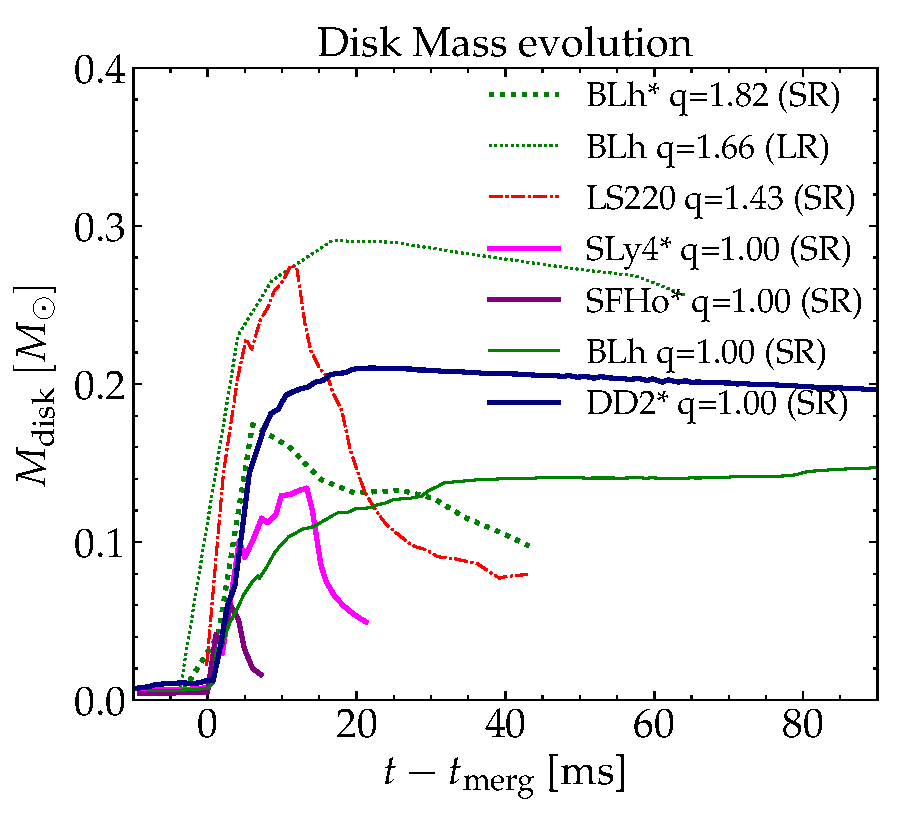
\includegraphics[width=0.49\textwidth]{disk/total_disk_mass_evo.pdf}
    \caption{
        Time evolution of the mass of the disk for a representative list 
        of simulations, that includes those that produce long-lived 
        remnants, \eg, DD2* $q=1.00$, short-lived remnants, 
        \eg, SLy4* $q=1.00$, and a simulation that undergoes \ac{PC}, 
        BLh* $q=1.82$. 
        %
        The plot shows that the \pmerg{} evolution of disk mass depends 
        strongly on the remnant. If the remnant is a \ac{NS}, the disk is 
        accreted slowly and its mass remains almost unchanged by the end 
        of our simulations, while if \ac{BH} forms, the disk is accreted 
        rapidly (if \mr{} is not large).
%        Time evolution of the total disk mass for a few selected
%        short-lived and long-lived cases. The former show a rapid 
%        accretion right after disk formation. The plots show
%        distinct difference in dynamical evolution after disk formation: accretion onto
%        the newly formed BH (short-lived remnants) or accretion onto the NS
%        remnant (DD2 $q=1$) with possible continuous mass shedding from the remnant
%        into the disk (BLh* $q=1$). 
        (Adapted from \citet{Nedora:2020pak}).
    } 
    \label{fig:disk_mass_evo}
\end{figure}


%
%These are the models with DD2 \ac{EOS} $q=1.00$ and BLh \ac{EOS} $q=1.00$.
%
Fig.~\ref{fig:ang_mom_flux} shows that the angular momentum is transported 
via spiral waves, induced by the $m=1$ and $m=2$ hydrodynamic modes, 
discussed above. We find the characteristic spiral wave structure 
in all our simulations. It smears out only if a \ac{BH} is formed.
%
In Fig.~\ref{fig:disk_ang_mom_flux_map_blh_q1} we show how the 
angular momentum is being transported from the \ac{NS} 
remnant into the disk 
%with its flux defined as $J_r = T_{ra}(\p_\phi)^a$
in two models with long-lived 
\ac{NS} remnants: %and included turbulent viscosity:
DD2* $q=1.00$ and BLh* $q=1.00$.
%
Notably, in the model with a more stiff DD2 \ac{EOS}, 
the first wave is considerably stronger. 

%Notably, the DD2 $q=1.00$ model also has a more massive disk.

%%%% MOVED DOWN
%The evolution of the disk-remnant interactions after ${\sim}20\,$ms \pmerg{} 
%is different for two models. While in the DD2* $q=1.00$ model the 
%accretion takes starts to dominate over mass shedding,
%in the BLh $q=1.00$ model the mass shedding prevails till 
%the end of the simulation.
%%shedding mass into its disk stops and accretion begins, in the model with BLh \ac{EOS} the mass shedding does not terminate 
%%continues to shed mass into the disk (see Fig.~\ref{fig:disk_mass_evo}).
%% and discussion in Sec.~\ref{sec:bns_dynsmics_overview})
%%
%The latter is caused by the strong angular momentum flux 
%%\red{actually the plot shows, that it is not}, 
%emanating from the \ac{NS} remnant.
%This might be attributed to the larger temperatures 
%that a model with BLh \ac{EOS} can reach (See Sec.~\ref{sec:nr_methods:eos}). 
%%
%Larger temperatures lead to lower rotational frequency at which the mass 
%shedding occurs \citep{Kaplan:2013wra}. 

The subgrid turbulence enhances the angular momentum transport. 
However, more simulations of long-lived 
\ac{NS} remnants are needed to assess the effects of the 
subgrid turbulence systematically. 


%\subsubsection{High \mr{} binaries}

%\subsection{The evolution of remnant-disk interactions}
%\subsection{Remnant-disk evolution}

%\subsubsection*{High mass ratio binaries}
%\subsection{High mass ratio binaries}

%% --- On THE PROMPT collapse
We find that in \ac{BNS} merger simulations with high \mr{}, $q\gtrsim1.67$, the companion star (the less 
massive one) undergoes tidal disruption before merger as tidal forces overcome the star's 
binding energy, creating a disk around the primary.
The disk accretion brings the remaining \ac{NS} mass above the 
maximum mass supported by its \ac{EOS}, which leads to a \ac{PC} 
of the remaining star. 
%These are so-called, prompt collapse cases \citep{Radice:2020ddv,Bernuzzi:2020tgt,Bernuzzi:2020txg}.
These \ac{BNS} models are characterized by a monotonic increase in their 
central density during the merger.
%The newly formed \ac{BH} is surrounded by the accretion disk that was 
%left from the tidally disrupted companion.
%
We also observe that at formation, the disk is massive, ${\sim}0.15\,\Msun$, in comparison with 
disks formed in \ac{PC} of equal mass binaries \citep[\eg][]{Radice:2018pdn}, 
and is also very neutron-rich, $Y_e\sim 0.1$.  
%
%and we discuss it separately for low \mr{} and high \mr{} binaries.
%The evolution of the disk mass is shown in Fig.~\ref{fig:disk_mass_evo}.

%\subsubsection*{Binaries with $q\lesssim1.4$}
%\subsection{Binaries with $q\lesssim1.4$}

Binaries with a small mass ratio, $q\lesssim1.4$,
produce either a short- or a long-lived remnant depending  
on the \pmerg{} configuration and properties. 
%produce a \ac{NS} remnant
%%that either survives on a dynamical timescale, set by the \ac{NS} rotation, before
%collapsing to a \ac{BH}, or a \ac{NS} remnant that survives till the end of the simulations.
%We refer to the former ones as \textit{short-lived} and the latter ones as %% ---------- Defind Above
%\textit{long-lived} remnants.
%
Most binaries that produce short-lived remnants have relatively soft \acp{EOS}
and small \mr{}s, \eg, models LS220 $q=1.1, \,q=1.2$, SFHo $q=1.1, \,q=1.4$, 
and SLy $q=1.1,\, q=1.4$. They collapse within ${\sim}20$~ms \pmerg. 
The exact time of the collapse, however, depends on the simulation resolution 
and on the inclusion of subgrid turbulence as was previously noted by \citet{Radice:2017zta}.






%\subsubsection*{Disk of short-lived remnants}
%\subsection{Disk of short-lived remnants}

%During the merger, shocks, generated at the collisional interface of the \ac{NS} cores,
%as well as, tidal torques exerted by the non axisymmetric remnant, result in a formation
%of the disk. Matter, energy and angular momentum are injected into the disk as the spiral 
%density waves propagate outwards from the mass-shedding \ac{NS} remnant 
%\citep{Bernuzzi:2015opx,Radice:2018xqa}.
%
%\red{HERE the letter stuff could be added, actually}
%
% --- Letter stuff
%The spiral arms extend from the \ac{NS} remnant into the disk and transport angular 
%momentum outwards as shown in Fig.~\ref{fig:ang_mom_flux}. %Such global density waves are --- written above 
%a generic and efficient mechanism to redistribute energy and eventually deplete  
%accretion disks \citep{Goodman:2001a,Rafikov:2016a,Arzamasskiy:2018a}. 
%% Crucially, we find that both the $m=1$ and $m=2$ modes generate a \wind{} from the
%% disk's outer layers that is distinct from the dynamical ejecta, see Fig.~\ref{fig:ej_properties}.
%
% <<< MOVED TO INTRO >>>
%
%The maximum values of fluid temperature in the disk are reached within 
%the spiral waves. During the \pmerg{} evolution, the disk expands and 
%cools via neutrino emission.
%High temperatures lead to the electron-positron pair creation, 
%%% [added from Shibata Review paper]
%facilitating the positron capture by free neutrons 
%%$n+e^+ \rightarrow p +\bar{\nu}_e$ 
%in the disk.
%%
%The average particle energies are large, close to the mass difference between neutron 
%and proton. 
%The entropy per baryon varies between $3$ and $\lesssim 10\,$$k_{B}$/baryon \citep{Perego:2019adq}.
%In combination with the high $\nu_e$ and $\bar{\nu}_e$ luminosities,
%the large number of available positrons leads to an increase 
%in the fluid electron fraction, $Y_e$, in relation to the initially neutron-rich material
%\citep{Qian:1996xt}.
%This process is called deleptonization. 
%%
%Additionally, a \ac{NS} remnant itself is a strong neutrino emitter. The neutrino irradiation of the 
%surrounding area alters its composition, as neutrons and protons absorb the neutrinos,
%$n+\nu_e\rightarrow p + e^{-}$ and $p + \bar{\nu}_e\rightarrow n + e^+$.
%This drives the neutron and proton fraction towards equilibrium, and raises the $Y_e$.
%%\red{paper says: 
%%    The electron fraction is reset by an initial excess of electron antineutrino emission
%%    and electron neutrino absorption,}
%% ---
As we discussed in Sec.~\ref{sec:intro:merg_pmerg}, the strong neutrino fluxes 
emanating from the remnant and the hot disk matter 
raise the fluid electron fraction. 
%
If a \ac{NS} remnant collapses to a \ac{BH}, the main source of neutrinos shuts down,  
the inner part of the disk accretes rapidly, and the disk itself moves to a 
quasi-steady state with axisymmetric and approximately Keplerian profile. 
%(see Fig.~\ref{fig:disk_mass_evo}).
%
Indeed, in our models we find that the inner part of the \pmerg{} disk, 
at densities $\rho\sim10^{13}\,$\gcm{}, is relatively hot, $T\sim10\,$MeV, 
but neutron-rich $Y_e\sim0.1$, as it is shielded from the neutrino irradiation. 
The matter gets progressively colder and proton-rich outwards, 
with $Y_e$ reaching $0.4$ at the disk edges.

%We display this behaviour for two representative models, 
We examine this behaviour in two representative models, 
BLh $q=1.00$ and LS220 $q=1.43$, where the former model was evolved till 
${\sim}90$~ms \pmerg{}. 
The evolution of the mass-weighted electron fraction in these models 
is shown in Fig.~\ref{fig:total_disk_time_corr_Ye_Blh_q1}. 
%
We observe that, during the disk formation, shocks and spiral waves raise the disk 
electron fraction to
$Y_e\sim0.25$. As the disk evolves, the bulk of its mass, shielded from neutrinos, 
%(Fig.~\ref{fig:slice:heating_hu}, density contours) 
returns to neutron-rich conditions with $Y_e\lesssim0.1$. The outer part of the disk, 
however, is subjected to strong neutrino irradiation and reaches $Y_e\sim0.4$ on a 
timescale of ${\sim}40$~ms\footnote{
    The apparent gap in the $Y_e$ distribution in 
    Fig.~\ref{fig:total_disk_time_corr_Ye_Blh_q1} at $\langle Y_e \rangle \simeq 0.15$ 
    might not be of physical origin, but an artifact from the neutrino M0 scheme 
    that assumes neutrinos propagate along the radial directions
    (see Sec.~\ref{sec:nr_methods:neut}). 
%    that is not well suited for capturing the 
%    neutrino emission and re-absorption from the disk midplane.
}.
%% Note that neutrinos in merger remnants decouple at $\rho\sim10^{11}$~$\gccm$ \citep{Endrizzi:2019trv}. 
%
In case of the LS220 $q=1.43$ models that produces a short-lived \ac{NS} remnant, 
the average electron fraction is lower, as the main source of neutrinos collapses 
shortly after merger.



The disk mass at formation shows dependency on the \ac{NS} \ac{EOS}. Specifically, 
binaries with stiffer \acp{EOS} (larger \ac{NS} radii) produce more massive disks. 
The disk mass also shows dependency on \mr{}. For instance, the most massive 
disks are formed in LS220 $q=1.43$ and BLh $q=1.82$ models.
%
The disk accretion onto a \ac{BH} removes up to 
$50\%$ of its mass on a timescale of tens of milliseconds.
%
%
%% -- 
%\subsubsection*{Disk of long-lived remnants}
%\subsection{Disk of long-lived remnants}
%
If the \ac{NS} remnant is long-lived, the disk has time to complete its formation,
and thus it is more massive and extended \citep{Perego:2019adq}. 
%As before, the disk is defined as matter, with $\rho\lesssim10^{13}$~\gcm. 
The final mass is higher for models with larger \mr{}s and stiffer \acp{EOS}.
For instance, 
in the BLh $q=1.00$ model
%for the model with $q=1.00$ and BLh \ac{EOS}, 
the disk mass reaches ${\lesssim}0.15\,\Msun$, while in the 
%model with $q=1.00$ and DD2 \ac{EOS} 
DD2 $q=1.00$ model 
it exceeds ${\sim}0.2\,\Msun$. For models with BLh \acp{EOS}, 
the disk mass increases between $q=1.00$ and $q\sim1.4-1.5$ by $100\%$.

%The evolution of the disk-remnant interactions after ${\sim}20\,$ms \pmerg{} 
%is different for two models. While in the DD2* $q=1.00$ model the 
%accretion takes starts to dominate over mass shedding,
%in the BLh $q=1.00$ model the mass shedding prevails till 
%the end of the simulation.
%%shedding mass into its disk stops and accretion begins, in the model with BLh \ac{EOS} the mass shedding does not terminate 
%%continues to shed mass into the disk (see Fig.~\ref{fig:disk_mass_evo}).
%% and discussion in Sec.~\ref{sec:bns_dynsmics_overview})
%%
%The latter is caused by the strong angular momentum flux 
%%\red{actually the plot shows, that it is not}, 
%emanating from the \ac{NS} remnant.
%This might be attributed to the larger temperatures 
%that a model with BLh \ac{EOS} can reach (See Sec.~\ref{sec:nr_methods:eos}). 
%%
%Larger temperatures lead to lower rotational frequency at which the mass 
%shedding occurs \citep{Kaplan:2013wra}. 

The long-term evolution of a disk is driven by its interaction with the \pmerg{} 
remnant, and by cooling. 
In Fig.~\ref{fig:disk_mass_evo} disk mass as a function of time for a set of 
models is shown. 
%
If a \ac{BH} forms, the only possible 
interaction is disk accretion onto a \ac{BH}, which leads to the depletion of the disk. 
However, if a remnant is a massive \ac{NS}, the picture is more complex.
%
Neutrino cooling and gravitational pull from the remnant facilitate  
accretion. Simultaneously, spiral density waves inject %generated at shocks,
energy and angular momentum into the disk, as well as centrifugally supported 
material, raising its temperature and geometrical extent.  %(the \ac{NS} remnant undergoes mass-shedding). 
This is the case for the DD2* $q=1.00$ and BLh $q=1.00$ models where the quasi-steady 
state disk accretion and mass-shedding maintain the disk mass almost constant 
until the end of the simulation. %, as depicted in Fig.~\ref{fig:disk_mass_evo}.
%
%In Fig.~\ref{fig:disk_mass_evo} the quasi-steady state disk accretion
%is seen for the DD2 $q=1.00$ model. Meanwhile, the mass-shedding 
%by the remnant adds more material into the disk than is being accretted as is the 
%case for the model with BLh \ac{EOS} and $q=1.00$. 
%
The strong mass-shedding in the BLh $q=1.00$ model can be attributed to the very 
high average temperatures of the remnant and the disk. % reached at merger. 
This is a direct consequence of the thermal effects included in the BLh \ac{EOS} 
(see Sec.~\ref{sec:nr_methods:eos}), and the softness of this \ac{EOS}, 
which leads to strong oscillations of the remnant after merger. 
%as discussed above. 
Higher temperatures lead to lower rotational 
frequency at which mass shedding occurs \citep{Kaplan:2013wra}. 
%(see Sec.~\ref{sec:bns_sims:dens_modes}).

When the subgrid turbulence is included, the mass distribution of the disk's 
properties appears smeared. The distributions of electron fraction, entropy per baryon and 
temperature appears broader. A more detailed quantitative analysis would require more 
simulations performed at several resolutions to disentangle the effects 
caused by the subgrid turbulence and by the finite grid  \citep{Bernuzzi:2020txg,Radice:2020ids}.


%%%%% <<< MOVED ABOVE
%\subsection{Evolution of disk properties and disk final structure}
%%\subsection{Evolution of disk properties}
%
%%% Ye evolution
%The evolution of the mass-weighted electron fraction in the 
%%the model with BLh \ac{EOS} and $q=1.00$, 
%BLh $q=1.00$ and LS220 $q=1.43$ models is shown in 
%Fig.~\ref{fig:total_disk_time_corr_Ye_Blh_q1}, 
%%
%where former model has been evolved till ${\sim}90$~ms \pmerg{}. 
%%
%During the formation, shocks and spiral waves raise the disk electron fraction to
%$Y_e\sim0.25$. As the disk evolves, the bulk of its mass, shielded from neutrinos, 
%%(Fig.~\ref{fig:slice:heating_hu}, density contours) 
%returns to neutron-rich condition with $Y_e\lesssim0.1$. The outer part of the disk, 
%however, is subjected to the strong neutrino irradiation and reaches $Y_e\sim0.4$ on a 
%timescale of ${\sim}40$~ms\footnote{
%    The apparent gap in the $Y_e$ distribution in 
%    Fig.~\ref{fig:total_disk_time_corr_Ye_Blh_q1} at $\langle Y_e \rangle \simeq 0.15$ 
%    might not be of physical origin, but an artifact from the neutrino M0 scheme, 
%    that assumes neutrinos propagate along the radial directions
%    (see Sec.~\ref{sec:nr_methods:neut}), that is not well suited for capturing the 
%    neutrino emission and re-absorption from the disk midplane.
%}.
%%% Note that neutrinos in merger remnants decouple at $\rho\sim10^{11}$~$\gccm$ \citep{Endrizzi:2019trv}. 
%%
%In case of a 
%LS220 $q=1.43$ models that produces a 
%short-lived \ac{NS} remnant  % model with LS220 \ac{EOS} and $q=1.43$ 
%(right panel of the Fig.~\ref{fig:total_disk_time_corr_Ye_Blh_q1})
%the average electron fraction is lower as strongly irradiating remnant the 
%collapses shortly after merger. 
%%
%%Additionally, the outskirts of the more compact disk remain 
%%at low electron fraction as the neutrino emitted by the disk itself 
%%%%are the only source of neutrinos. 

%\end{document}

%% -----------------------------------------------
%%
%% F I N A L  D I S K  S T R U C T U R E
%%
%% -----------------------------------------------

\subsection{Final disk structure}
%\subsection{Final disk structure}

\begin{figure}[t]
    \centering
    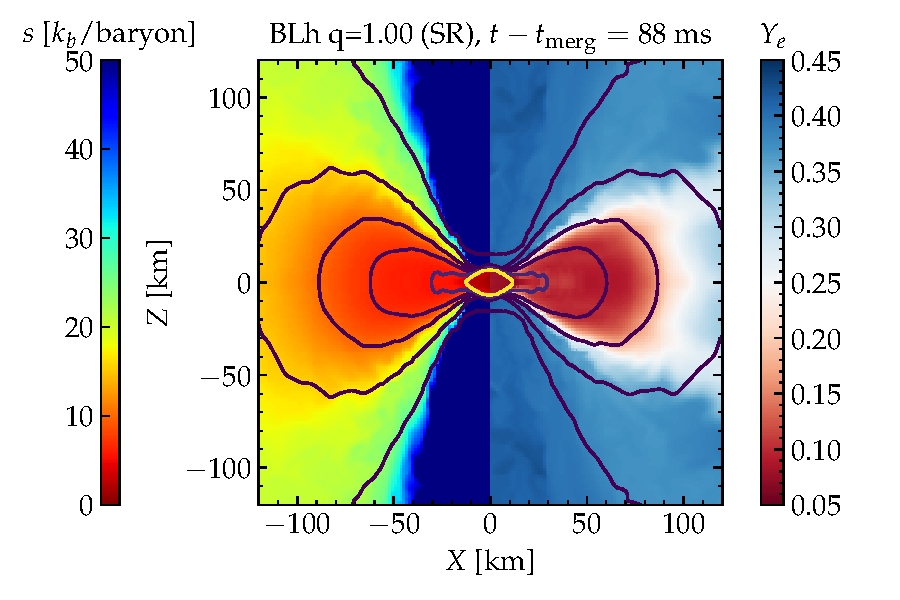
\includegraphics[width=0.49\textwidth]{disk/final_structure/slice_xz_entr_ye_blh_q1_rl3.pdf}
    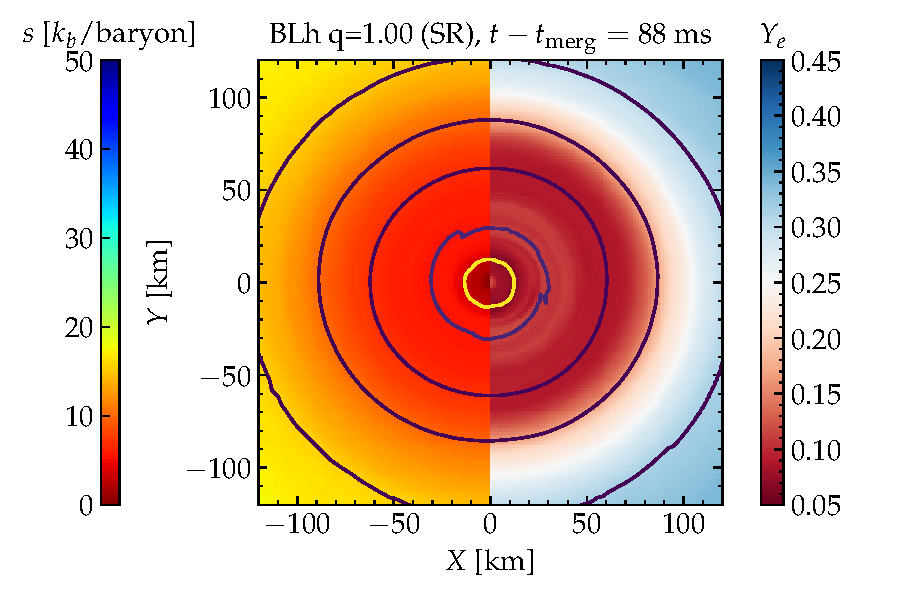
\includegraphics[width=0.49\textwidth]{disk/final_structure/slice_xy_entr_ye_blh_q1_rl3.pdf}
    \caption{
        Snapshots of disk properties on $(x,z)$ \textit{left panel} and 
        $(x,y)$ \textit{right panel} for the BLh $q=1.00$ model, taken 
        $88\,$ms \pmerg{}. 
        %
        On each panel, the entropy per baryon is shown on the left 
        side of the panel, and the electron fraction on the right. 
        %
        Solid contours mark the rest mass density values, which read $[10^{13}, 10^{12}, 10^{11}, 10^{10}, 10^{9}]$ g cm$^{-3}$ from the innermost yellow contour encompassing the remnant.
        (Adapted from \citet{Nedora:2020pak}). 
%        Entropy and electron fraction on the $(x,z)$ (top) and
%        $(x,y)$ planes (bottom) for the remnant of BL $q=1$ at the end
%        of the simulation. Each plot is divided vertically, with entropy
%        being color-coded on the left and electron fraction on the
%        right. Solid contours stand for rest muss density. Counting from
%        the center, the values are $[10^{13}, 10^{12}, 10^{11}, 10^{10},
%        10^{9}]$ g cm$^{-3}$, with the inner most contour encompassing
%        the remnant.
%        (Adapted from \citet{Nedora:2020pak})
    }  
    \label{fig:snapshots_xy_ye_entr}
\end{figure}

\begin{figure*}[t]
    \centering 
    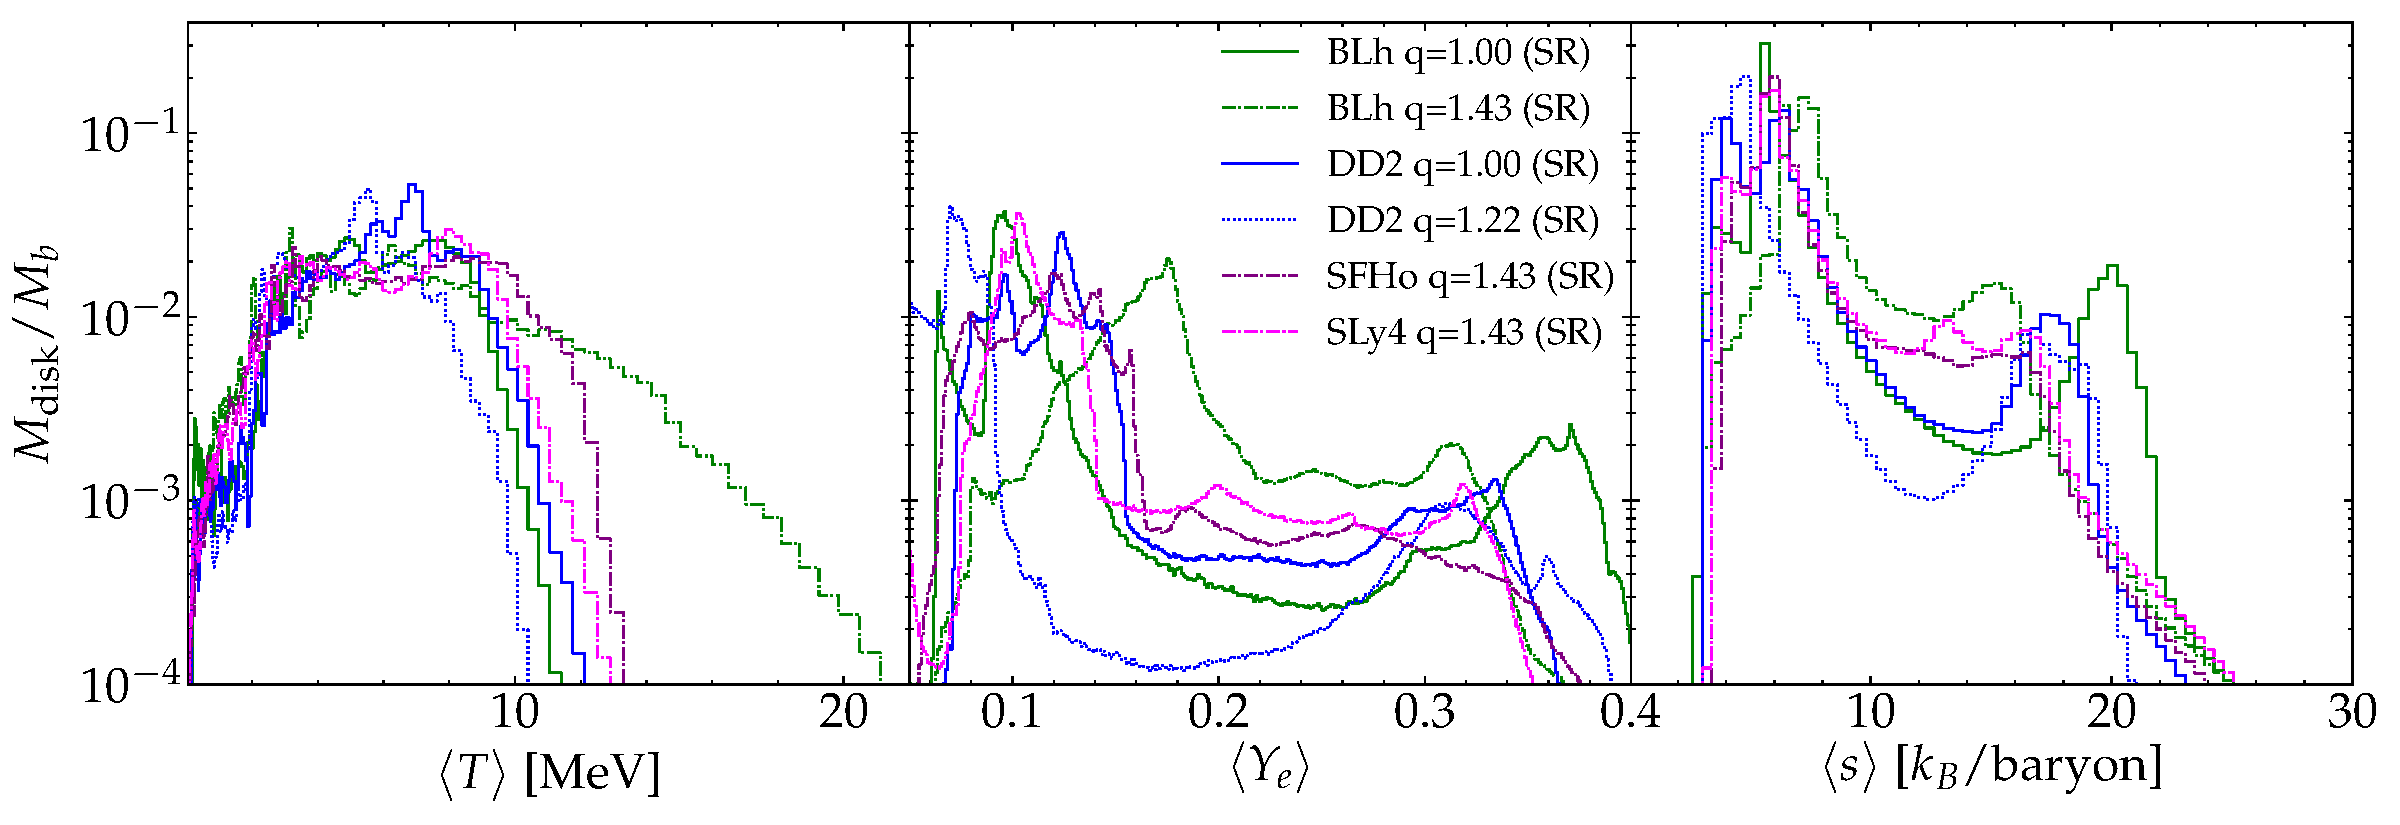
\includegraphics[width=0.95\textwidth]{disk/final_structure/disk_hist_shared.pdf}
    \caption{
        Disk properties in the form of mass histograms 
        at the end of evolution for a set of simulations.
        From left to right, panels depict the temperature, $T$, 
        fraction $Y_e$ and entropy $s$. 
        (Adapted from \citet{Nedora:2020pak}).
%        \textit{Left panel} shows the temperature, $T$, 
%        \textit{middle panel} depicts the, 
%        
%        Composition of the disks at the end of the long-lived
%        remnants simulations. The histograms refer to the temperature $T$
%        (left),
%        electron fraction $Y_e$
%        (middle) and entropy $s$ (right).
%        (Adapted from \citet{Nedora:2020pak})
    }
    \label{fig:final_disk_struct_hist_long}
\end{figure*}

%In this section we discuss the final structure and properties of the disk, 
%focusing on the models with long-lived \ac{NS} remnants.
%The properties are extracted at typical time $\sim60{-}100$~ms after merger.
%
From the density contours in Fig.~\ref{fig:snapshots_xy_ye_entr}, 
we observe that even at ${\sim}88\,$ms after merger the disk
of the BLh $q=1.00$ model remains geometrically thick. 
%We find that the generally the disk is optically thick.
Comparing with other models, we note that 
the \ac{RMS} half-opening angle of the disk appears to be independent of the 
\ac{EOS} and \mr{}, and is $\langle\theta\rangle_{\text{rms}}\sim60^{\circ}$. 
The radial extent of the disk, however, increases with the \ac{EOS} softness and $q$.
%
Similarly, the final disk mass is larger for the unequal mass binaries, 
ranging overall between ${\sim}0.1\,\Msun$ and ${\sim}0.4\,\Msun$
(see Tab.~\ref{tab:sim}), and is larger in models that produce long-lived remnants.

%
We examine disk mass dependencies on binary parameters in Appendix~\ref{ch:stat}, 
Sec.~\ref{sec:stat:remdisk}, where we combine our data with the data available in 
the literature (see Sec.~\ref{sec:bns_sims:ejecta}) 
and show that the aforementioned dependencies on $q$ and $\tilde{\Lambda}$ 
can be captured by a simple two parameter, second order polynomial in 
these quantities. 
We find that in comparison with other fitting 
formulae available in the literate the polynomial performs better. 
%
The systematics in data, however, are large. 
More \ac{BNS} merger simulations with advanced physics and a consistent method 
of disk mass extraction are required for constraining the polynomial, 
especially at the known boundaries of the parameter space, 
\eg, $\tilde{\Lambda}\rightarrow0$.


%than short-lived ones as \ac{BH} accretion removes ${\sim}50\%$ 
%of the mass in the latter case.
%
%Notably, for models with long-lived remnants the disk mass is larger,
%that for the those with short-lived remnants. This can be attributed to the 
%rapid accretion onto a \ac{BH} that removes $\sim50\%$ of the disk mass.
%
%We investigate the overall statistical properties of the disk mass for all our models
%and compare them to those available in the literature in Sec.~\ref{sec:stat:remdisk}
%
%\gray{
%    The mean value of the disk mass in out models is 
%    $\overline{M}_{\text{disk}}=(0.161 \pm 0.083)M_{\odot}$,
%    where the standard deviation is also reported.
%    %% ---
%    Similarly to the dynamical ejecta we fit the disk masses with the 
%    second order polynomial in $(q,\tilde{\Lambda})$.
%    The coefficients of Eq.~\eqref{eq:fit:poly22}
%    for this fit are given in Tab.~\ref{tab:fitpoly22coefs}.
%    A more detailed study with various fitting formulas and extended
%    datasets from the literature is reported in a companion paper.
%}

%Next, we consider the composition of the disk at the end of the simulation.
%
The mass-averaged temperature, electron fraction and entropy per baryon
for several models are presented in Fig.~\ref{fig:final_disk_struct_hist_long}.
%
The plot shows that the mass-weighted distribution of entropy and the electron 
fraction have a bimodal structure, which is more pronounced in the case of 
equal mass binaries. 
The low entropy, $s\sim5-10\,k_B/$baryon, peak corresponds to the bulk, 
mildly shocked 
material, while the higher entropy peak, $s\sim15-22\,k_B/$baryon, marks 
the strongly shocked material. Notably, the low entropy peak is largely 
independent of the \ac{EOS} and \mr{}, while the high entropy peak is more pronounced 
in models with softer \acp{EOS}. 
%
%
%Notably, in models with higher \mr{}, 
%the second peak is located at lower $s$. 
%
%The mass-weighted distribution 
%of the electron fraction displays a similar double-peak structure.
Similarly, the low $Y_e$ peak, $Y_e\sim0.1$, corresponds to the neutrino-shielded part of the 
disk, while the high $Y_e$ peak, $Y_e\sim0.3-0.4$, marks the outer parts of the disk,
where fluid is subjected to strong neutrino irradiation.

Comparing the disk properties with the 2D snapshots of the electron fraction 
and density within the disk, 
shown in Fig.~\ref{fig:snapshots_xy_ye_entr}, we observe 
that indeed, the two peaks in the mass-weighted distribution of 
$s$ and $Y_e$ correspond to different regions within the disk.
%
%In Fig.~\ref{fig:snapshots_xy_ye_entr} we show the electron fraction 
%and entropy per baryon on the $xy$ and $xz$ slices of the equal 
%mass model with BLh \ac{EOS}. The plot shows, that the two peaks in the 
%mass-weighted distribution of electron fraction and entropy correspond to 
%different regions within the disk.
%
Similarly, we observe that the innermost parts of the disk are hotter 
than the outermost ones. The bulk of the disk has $T\sim 1-10\,$MeV. 
The disk temperature distribution appears to be largely 
independent of the \ac{EOS} and \mr{}.




%% -----------------------------------------------
%%
%% E X P E C T E D  M A S S  E J E C T I O N
%%
%% -----------------------------------------------

%\subsection{Mass ejection on a longed timescale}
\subsection{Mass and angular momentum loss}\label{sec:bns_sims:mj_loss}

%As the disk expands and cools, the recombination of nucleons into alpha particles 
%starts to take place. The energy, released in recombination, might be sufficient 
%for the outermost layers to become unbound, generating an outflow and contributing 
%to the disk depletion \citep{Beloborodov:2008nx,Lee:2009uc,Fernandez:2013tya}.
%%
%This process, however, is expected to take place on timescales longer than
%those simulated here. 
%Additionally, an outflow induced by viscous heating within the disk and 
%so-called neutrino-driven wind (\nwind{}; \citet{Dessart:2008zd,Perego:2014fma,Just:2014fka})
%driven by neutrino heating above the remnant, are expected to contribute to the 
%mass and angular momentum mass loss. 

%and by the dynamical
%interactions between the \ac{NS} remnant and the disk, the \swind{} \citep{Nedora:2019jhl}.
%
%We discuss the properties of the ejecta in the next section, 
%Sec.~\ref{sec:bns_sims:ejecta}.

%We discuss the properties of the \nwind{} found in our simulations
%in Sec.~\ref{sec:bns_sims:nwind} and the properties of the 
%\swind{} in Sec.~\ref{sec:bns_sims:sww}.
%
%The \swind{} can have a mass up to
%a few $10^{-2}\,\Mo$ and velocities ${\sim}0.2$~c. The ejecta
%have electron fraction typically larger than ${\sim} 0.25$ since they are 
%partially reprocessed by hydrodynamic shocks in the expanding arms. 
%The \nwind{} is driven by neutrino heating above the remnant. It generates outflows
%with smaller masses ${\sim} 10^{-4}M_{\odot}$ and larger $Y_e$
%than the \swind{}. 
%Differently from \swind{} the mass flux of the \nwind{} in our simulations subsides 
%before the end of out simulations, due to rapid baryon loading of the 
%polar region.
%The \swind{} will be discussed in detail in Sec.~\ref{sec:spiralw}.
%The effects of these outflows on the dynamical evolution of the remnant 
%lies in the amount of mass and angular momentum they can remove from the system.
%
%Specifically, the \nwind{} have a typical mass of ${\sim} 10^{-4}\,\Msun$, 
%while the \swind{} could remove $10^{-2}\,\Msun$ on a timescale of a ${\sim}100\,$ms.

\begin{figure}[t]
    \centering 
    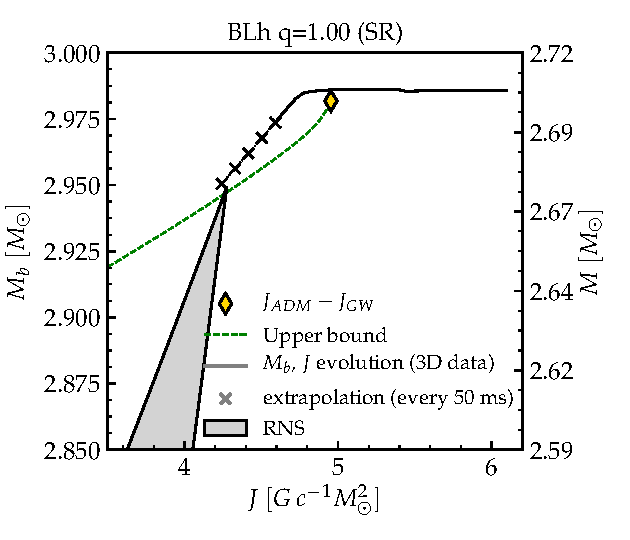
\includegraphics[width=0.59\textwidth]{ejecta_sec/secular_j_mb_RNS_blh.pdf}
    \caption{
        Evolution of the BLh $q=1.00$ \pmerg{} remnant $J$-$M_b$ space, where 
        $J$ is the total angular momentum and $M_b$ is the baryonic mass, 
        depicted by the solid black line. The evolution begins in the 
        upper right corner and proceeds towards the lower left one, as the 
        remnant loses first angular momentum to \ac{GW} emission, then 
        both $J$ and $M_b$ to massive winds. The point where the \ac{GW}-phase 
        ends is marked with yellow marker. 
        The end of the solid black line indicates the end of our simulation. 
        We linearly extrapolate the evolution trajectory, and plot it with black crosses. 
%        Baryon mass vs angular momentum diagram for the BLh $q=1$ remnant.
%        The colored diamond marks the baryonic mass and angular momentum at the end
%        of the dynamical gravitational-wave dominated phase.
%        After the GW phase, the evolution is driven by the massive outflows.
%        The solid black line is the $M_b$ and $J$ estimated from the 3D data
%        integrals under the assumption of axisymmetry.
        The green dashed line is a conservative estimate
        of the mass ejection and a possible trajectory for the viscous
        evolution as estimated in \citet{Radice:2018xqa}. 
%        The crosses are
%        a linear extrapolation in time of the solid black line. 
        The gray
        shaded region is the region of stability of rigidly rotating \ac{NS} 
        equilibria. 
        (Adapted from \citet{Nedora:2020pak}).
    }
    \label{fig:total_j_mb_rns_blh}
\end{figure}
%        \footnote{
%            \url{http://www.gravity.phys.uwm.edu/rns/#:~:text=RNS%20is%20a%20code%20written,are%20supplied%20by%20the%20user.}
%        }
Quantitative understanding of the long-term \pmerg{} dynamics 
requires ab-initio \ac{NR} simulations in $(3+1)$D with complete physics.
%
Here we assess a possible long-term evolution via an indirect method, 
focusing on the BLh $q=1.00$ (\texttt{SR}) model, one of the longest runs 
performed. 

In this simulation, after the merger, a \ac{NS} remnant is born with an excess 
in baryon mass with respect to the beta-equilibrium \ac{NS} configurations.
%
In Fig.~\ref{fig:total_j_mb_rns_blh} we show the evolution of the 
total baryonic mass, $M_b$, and total angular momentum, $J$ (the solid black line),  
%, of this remnant (black solid line). 
%
evaluated in cylindrical coordinates assuming axisymmetry and accounting for 
matter in the remnant and in the disk. 
%(see Eq.~\eqref{eq:method:ang_mom} and Eq.~\eqref{eq:method:mdisk},
%in Sec.~\ref{sec:bns_sims:method:ang_mom} and Sec.~\ref{sec:bns_sims:method:disk} respectively for more details).
%
%(for the definition of the latter see Sec.~\ref{sec:bns_sims:method:ang_mom}).
%
At early \pmerg{}, before any substantial mass-loss could occur, the 
evolution is governed by the emission of \acp{GW}. The remnant loses 
angular momentum but retains constant baryonic mass.
%
In order to evaluate the total amount of angular momentum lost to 
\acp{GW} we perform the frequency-domain integration of the \ac{GW} 
strain with the extraction sphere of $R=400\,\Msun$ using the 
\texttt{strain.py} module of the public library 
\texttt{scidata}\footnote{\url{https://bitbucket.org/dradice/scidata}}.
The method is discussed in 
\citet{Damour:2011fu,Bernuzzi:2012ci,Bernuzzi:2015rla}.
%
%\citet{Damour:2011fu,Bernuzzi:2012ci,Bernuzzi:2015rla}\footnote{
%    The radiated angular momentum is computed from the 
%    multipole moments $N_{lm}$ for the \ac{NR} complex "news function" at infinity. 
%    The $J_{z;\text{rad}}(t)$ is computed as \citep{Damour:2011fu} 
%    \begin{equation*}
%    \Delta J_{z\text{rad}}(t) \frac{1}{16}\sum_{l,m}^{l_{max}}\int_{t_0}^{t} dt' m \mathcal{L}[h_{lm}(t')(N_{lm}(t'))^*],
%    \end{equation*}
%    where $h_{lm}$ is the multipolar metric waveform, 
%    $N_{lm}(t) = dh_{lm}(t) / dt$, the news function, and $l_{max}=8$.
%    The $J$ loss is metric dependent ($h$).
%    The $h$ (strain???) is computed from $\Psi_4(t) = dN/dt = d^2h/dt^2$ by a 
%    frequency-domain integration procedure with a low-frequency cut 
%    $\omega_0 = 0.032/(m_1+m_2)$.
%    The routines used for the calculation are taken from the scientific library
%    \texttt{scidata}, available at \url{https://bitbucket.org/dradice/scidata}.
%}.

Subtracting the angular momentum lost to \acp{GW} from the initial data, 
%\ac{ADM} angular momentum,  %\red{(see \url{https://arxiv.org/pdf/1001.5429.pdf})} 
we obtain the value that is left to the system after the \ac{GW} phase 
(the yellow marker in Fig.~\ref{fig:total_j_mb_rns_blh}\footnote{
    Due to different assumptions in its calculation the agreement 
    with $J$ from the volume integrals is not expected.
}).
%
We observe that at this stage the remnant still has an excess in angular momentum
in comparison with the rigidly rotating \ac{NS} configurations with the same baryon mass 
(the gray triangular region in Fig.~\ref{fig:total_j_mb_rns_blh}).
%
The equilibria configurations were computed using the \texttt{RNS} 
public code \footnote{
    \texttt{RNS} is a code written by Nikolaos Stergioulas which constructs 
    models of rapidly rotating, relativistic, compact stars using tabulated 
    \ac{EOS} \url{http://www.gravity.phys.uwm.edu/rns/}.
}.
%
%Similar situation is found for other 
We observe the same situation in all our models.% \citep{Zappa:2017xba,Radice:2018xqa}.

Notably, the baryonic mass of the \pmerg{} remnant also exceeds 
the maximum mass that a rigidly rotating equilibria could have. 
As we mentioned in Sec.~\ref{sec:intro:merg_pmerg}, such a remnant is 
generally referred to as a \ac{HMNS} \citep{Baumgarte:1999cq} 
% following the 
%nomenclature introduced for zero-temperature \ac{EOS} equilibria \acp{NS} \citep{Baumgarte:1999cq}, 
and is expected to collapse to a \ac{BH} shortly after formation. 
%
However, as Fig.~\ref{fig:total_j_mb_rns_blh} shows, a remnant that efficiently 
loses mass sets on a trajectory towards the rigidly rotating, stable configuration. 
%
The extrapolation of the final trend of the mass and angular momentum loss 
suggests that if ${\approx}0.05\,\Msun$ 
(${\approx}40$\% of the final disk at the end of the simulation) is 
ejected, a \ac{NS} remnant would approach the rigidly rotating equilibria region 
at the mass-shedding limit. % (gray-shaded region in Fig.~\ref{fig:total_j_mb_rns_blh}). 
%
For the BLh $q=1.00$ model, if the ejecta mass flux does not change, 
the equilibrium would be reached within ${\sim}350$~ms \pmerg{}. 
%
%Extrapolation indicates, that if the ejecta mass flux does 
%not change, this would occur on a timescale of ${\sim}350$~ms \pmerg{}.
%
Thus, in principle, a \ac{HMNS} remnant could avoid collapse. 
This calls for a more detailed investigation with long-term \ac{NR} \ac{BNS} 
merger simulations that employ advanced physics.

%
%However, as Fig.~\ref{fig:total_j_mb_rns_blh} shows, the remnant that efficiently 
%losses mass, can avoid the collapse, if the \ac{RNS} concan avoid the 
%collapse by efficiently removing angular momentum and mass, and can reach the 
%rigidly rotating equilibria phase.% in a ${\sim}350\,$ms.
%avoiding the collapse.
%
%
%We compute the angular momentum and baryon mass evolution of the remnant 
%through volume integrals, assuming axisymmetry and evaluating the former using 
%Eq.~\eqref{eq:method:ang_mom}, and the latter using the Eq.~\eqref{eq:method:mdisk},
%relaxing the rest-mass density criterion. 
%The evolution of these two quantities is depicted with the black solid line if 
%Fig.~\eqref{fig:total_j_mb_rns_blh}~\footnote{
%    Note that the angular momentum estimated
%    from the \ac{GW} and from the integral of Eq.~\eqref{eq:method:ang_mom} assuming
%    axisymmetry are compatible within the errors made in the latter estimate.
%}.

The massive outflow that starts to dominate the \pmerg{} dynamics after the \ac{GW}-phase, 
is driven by the interaction between the non-axisymmetric 
remnant, subjected to $m=1$ and $m=2$ instabilities, and the disk.
We call this ejecta \ac{SWW}. 
The properties of \ac{SWW} are discussed in the next section. 

%
%
%Similar results are obtained with the conservative upper bound estimate on the 
%evolution of the long-lived remnant (Eq.~$2$ in \citet{Radice:2018xqa}) (green dashed line in 
%the figure). 

Additionally, we estimate a conservative upper bound evolution of the 
long-lived remnant based on the following considerations \citep{Radice:2018xqa}.
%
%%%% From Radice18 paper on ViscousEjecta
%A more conservative estimate can be obtained assuming
%that the material becomes unbound due to the recombination
%of nucleons into nuclei and the subsequent liberation of
%nuclear binding energy, a scenario discussed in detail in 
%Beloborodov (2008), Lee et al. (2009), and Fernandez \& Metzger
%(2013), among others. This has been shown to occur
%once the material has reached a cylindrical radius $r*$ at
%which the nuclear recombination energy equals the gravitational
%binding energy (Lee et al. 2009; Fernandez & Metzger 2013), that is
%
%\begin{equation}
%    \frac{G M m_b}{r*} \approxeq 8.8\, \text{MeV}
%\end{equation}
%
%In the previous equation $M$ is the central object mass and
%$m_b$ is the average baryon mass. Accordingly, a ring of material
%initially orbiting at radius $r < r*$ and becoming unbound
%would carry away, in addition to its specific angular
%momentum $j(r)$, also the angular momentum needed to expand
%to $r*$. Assuming a Keplerian disk, this implies that
%the angular momentum carried away by the ring initially at
%$r$ is
%
%\begin{equation}
%    j*(r) = j(r) \Big( \frac{r*}{r} \Big)^{1/2}
%\end{equation}
%
%We take $r* = 300 G/c^2M$ as fiducial value, corresponding
%to $M \approxeq 2.5M_{\odot}$. We repeat the tally of angular momentum
%and mass that can be removed from the remnant
%taking into account the previous equation. The results are
%represented by the blue line in Fig. 3 laying inside the allowed
%region for the viscous evolution. This yields an ejecta
%mass of ${\sim}0.05\Msun$for the DD2 (1.35 + 1.35)$\Msun$ binary.
%Our estimate is in good agreement with the results of Fujibayashi
%et al. (2018), who considered the post-merger evolution
%of the same binary with 2D axisymmetric viscous
%GRHD simulations. They estimated the viscous ejecta mass
%to be ${\sim}0.05\Msun$. Note, however, that the mass ejection was
%still ongoing at the end of the simulations presented by Fujibayashi
%et al. (2018), so the total ejecta mass might be
%larger than what they estimated.
The recombination of nucleons into nuclei and the subsequent 
liberation of nuclear binding energy can be a driving force 
behind massive outflows (see Sec.~\ref{sec:intro:ejecta}). Matter becomes unbound gravitationally 
once it reaches cylindrical radius $r^*$, at which point the nuclear recombination 
energy becomes equal to the gravitational binding energy
\citep[\eg][]{Fernandez:2013tya}, 
%
\begin{equation*}
    G M m_b / r^* \simeq 8.8\, \text{MeV}, 
\end{equation*}
%
where $M$ is the central object mass and $m_b$ is the average baryon mass.
Thus, a ring of material located at $r < r^*$ would, once it becomes unbound, 
remove the angular momentum required to reach
to $r^*$,  in addition to its specific angular momentum $j(r)$.
% Thus, a ring of material located at $r < r^*$, once it becomes unbound,
% would remove in addition to its specific angular
% momentum $j(r)$, also the angular momentum required to reach
% to $r^*$. 
If the disk is Keplerian, the angular momentum carried away by 
the ring initially at $r$, is 
%
%\begin{equation*}
    $ j^*(r) = j(r) ( r^* / r )^{1/2}\, ,$
%\end{equation*}
%
where $ r^{*} = 300 G / c^2 M \,$ is the fiducial value, corresponding
to assumed total mass $M \approxeq 2.5M_{\odot}$ \citep{Radice:2018xqa}.
The expected trajectory is shown as the green line in Fig.~\ref{fig:total_j_mb_rns_blh}.
%
This analysis further suggests that sufficiently massive outflows 
can bring \pmerg{} \ac{HMNS} remnants to stability. 

%Additionally, while this simulation included the effects of turbulent viscosity on the
%angular momentum transport, the matter outflow could be further enhanced by the magnetic stresses 
%\citep{Metzger:2006mw,Bucciantini:2011kx,Siegel:2017nub,Fernandez:2018kax,Ciolfi:2020hgg}.
%
%
Our other simulations also produce \ac{NS} remnants with similar evolutionary paths. 
Models with the DD2 \ac{EOS}, however, are born with an excess in angular momentum but not in 
baryonic mass. They also evolve towards the rigidly rotating equilibria, but more slowly. 
Models with $q>1.00$ produce remnants that generally have larger excess in angular momentum 
and mass. They have to shed a larger amount of mass to reach an equilibrium configuration.
%(\red{However we also show that these models tend to have stronger \swind{}, see sec.SPIRAL.WIND})
Overall, we estimate that models with $q=1.00$ need to shed ${\sim}0.05\,\Msun$ while 
models with $q\eqsim 1.4$ need to remove $0.2\,\Msun$ to reach such a configuration.















%% ===================================================================================
%%
%%               E J E C T A
%%
%% ====================================================================================

\section{Mass ejection in BNS merger simulations} \label{sec:bns_sims:ejecta}

%% \section{Results -- Mass Ejection}


%Tidal interactions and shocks exerted on the \acp{NS} at merger 
%trigger the ejection of material on the dynamical timescale. This is the \ac{DE} 
%\citep[\eg][]{Hotokezaka:2013b,Bauswein:2013yna,Radice:2016dwd,Radice:2018pdn}. 
%\red{a bit more}



\subsection{Dynamical Ejecta} \label{sec:bns_sims:dyn}

%\red{EJECTA to be moved to its own section}
%The models that undergo the prompt collapse also eject matter on a dynamical timescale. 
%The ejecta originates from tidal disruption of the compantion. It is neutron rich, 
%confined largely to the orbital plane and exhibits a crescent-like azimuthal structure \citep{Bernuzzi:2020txg}.


%% The mechanism behind the dynamical ejecta [radice:2018pnd]
%Tidal interactions and shocks exerted on the \acp{NS} at merger trigger the ejection of material
%on the dynamical timescale. This is the \ac{DE} \citep[\eg][]{Hotokezaka:2013b,Bauswein:2013yna,Radice:2016dwd,Radice:2018pdn},
%composed of the tidal an shocked components.
%(see also Sec.~\ref{sec:intro:merg_pmerg} \red{INTRO?}).
%\red{More on the genral mechanism tidal vs shocked}
%The \ac{DE} is evaluated with the geodesic criterion introduced in Sec.~\ref{sec:method:analysis:ejecta}.
%
%Describe shock vs tidal components 
%
%
%%%% <<< MOVED TO INTRO >>>
%When \acp{NS} collide and merger, matter is ejected through a number of 
%different physical processes, gaining enough energy to become graviationally 
%unbound (according to the criteria discussed in Sec.~\ref{sec:bns_sims:method:ejecta}). 
%%\alpedit{The matter ejected on dynamical timescale of the system (${\sim}10$~ms) 
%%is called the dynamical ejecta.}{
%In particular, the matter ejected within a few dynamical timescales (\ie, ${\sim}10$~ms) 
%after merger by tidal torques and hydrodynamics shocks driven by core bounces 
%is called \ac{DE} \citep[\eg][]{Hotokezaka:2013b,Bauswein:2013yna,Radice:2016dwd,Radice:2018pdn}. 
%%
%% From AFTERGLOW paper
%%
%Several mechanisms contribute to the ejection, and depending on the 
%binary parameters, their relative contribution differs.
%%
%For instance, shortly before and during the merger, the outer parts 
%of the \acp{NS}, opposite to the collisional interface, are stripped 
%away by the tidal torque and centrifugal forces. This is the tidal 
%component of the \ac{DE}. It is more massive in binaries with 
%larger \mr{} and is maximum in those that experience tidal disruption 
%\citep[\eg][]{Radice:2018pdn,Bernuzzi:2020txg}.
%%
%Such ejecta is neutron rich, confined largely to the orbital plane and exhibits 
%a crescent-like azimuthal structure \citep{Bernuzzi:2020txg}.
%%
%Overall, the tidal ejecta component is mostly equatorial and its 
%velocity is related to the \acp{NS}' velocity at merger and 
%and the system's escape velocity, and is $\sim0.2$~c.
%%
%When \acp{NS}' cores collide and bounce, shocks propagate outwards inducing 
%matter ejection. Additionally, a small amount of material at the 
%\acp{NS}' collisional interface is shock-heated and launched into the polar 
%direction. This comprises the shocked component of the \ac{DE}.
%%
%It is more massive and faster if \acp{NS}' radii are smaller and they collide 
%at higher velocities \citep[\eg][]{Radice:2018pdn}. 
%%
%The dynamical ejecta has a broad distribution in terms of composition, 
%velocity and mass, dependent on the parameters of the binary and \ac{NS} \ac{EOS}.
%%% === ON THE FAST DYNAMICAL EJECTA IN PARTICULAR ===========


\begin{figure*}[t!]
    \centering 
    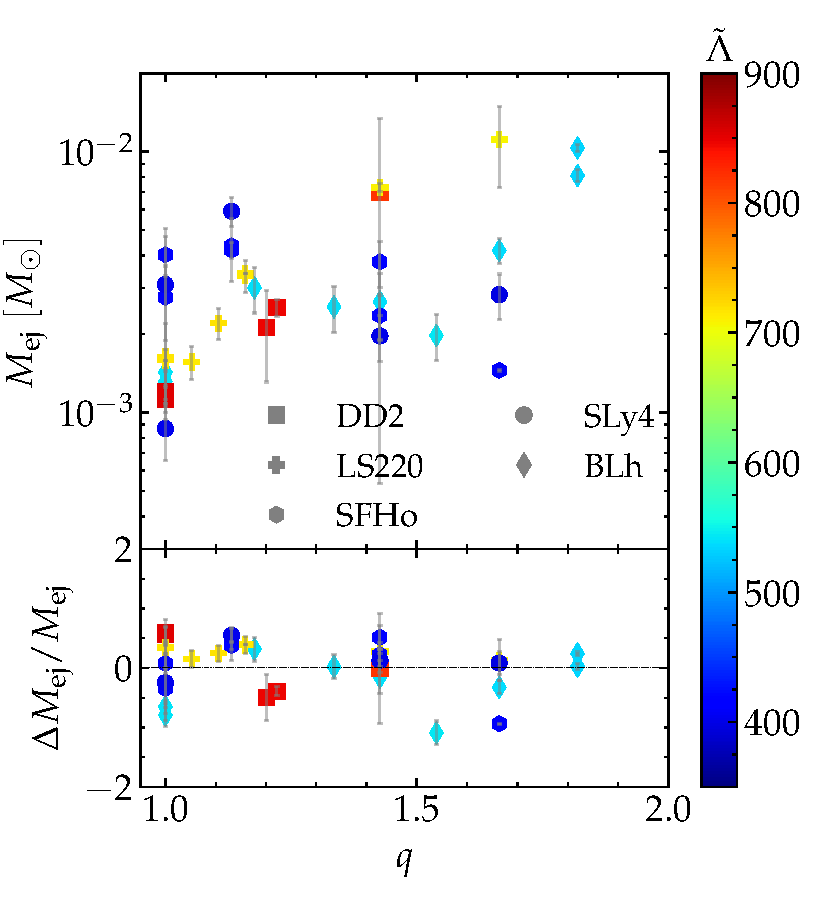
\includegraphics[width=0.49\textwidth]{statistics/ej_q_mej_our_poly22_cc.pdf}
    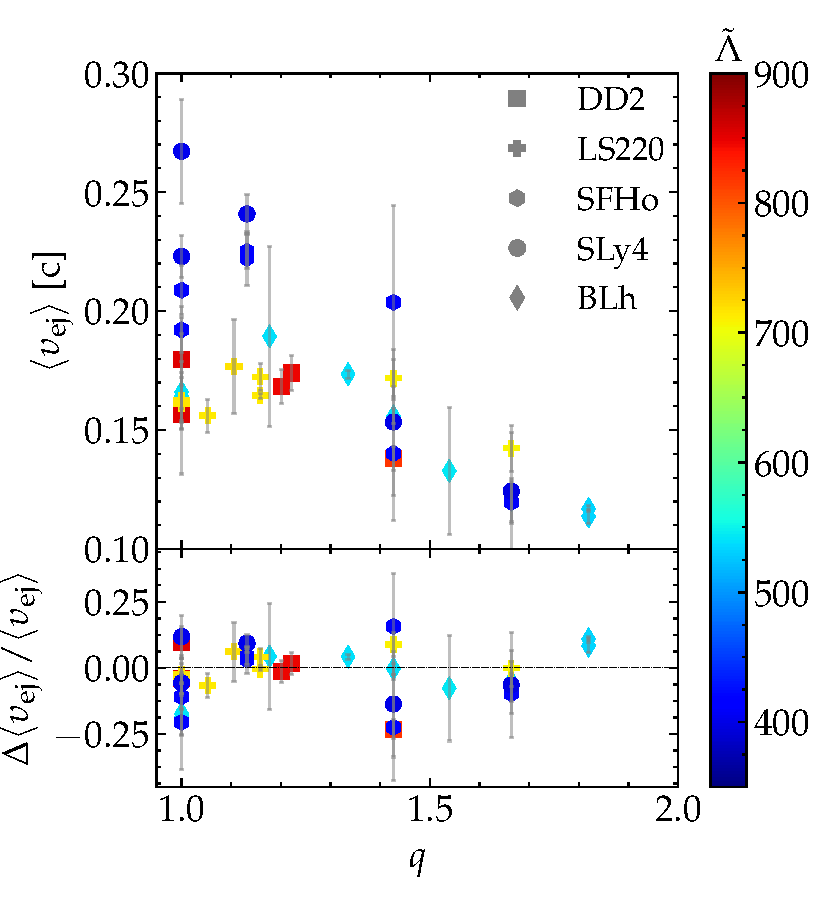
\includegraphics[width=0.49\textwidth]{statistics/ej_q_vej_our_poly22_cc.pdf}
    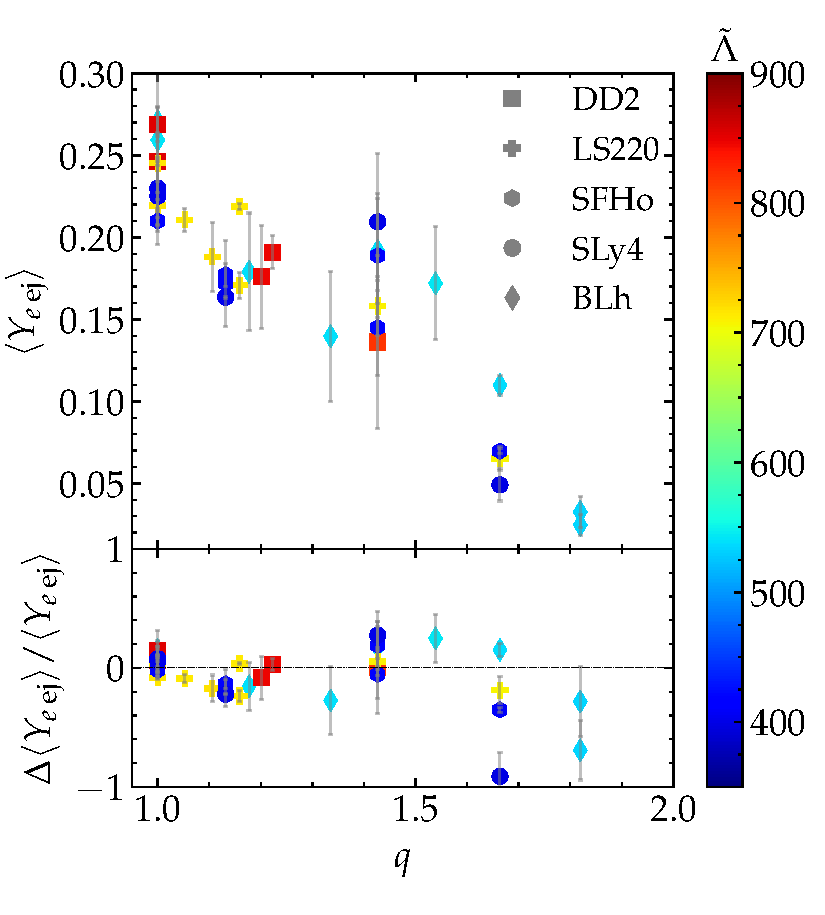
\includegraphics[width=0.49\textwidth]{statistics/ej_q_yeej_our_poly22_cc.pdf}
    \caption{
        \ac{DE} properties from our simulations as functions of binary parameters $q$ and $\tilde{\Lambda}$. 
        The \textit{first}, \textit{second} and \textit{third} \textit{panels} show 
        the mass, mass-averaged velocity and electron fraction respectively. 
        %
        In each panel, the lower suplot shows the relative difference 
        between the data and values inferred from the polynomial fitting 
        formula (see the text). 
        %
        (Adapted from \citet{Nedora:2020pak})
%        Dynamical ejecta properties as a function of mass ratio
%        and reduced tidal parameter. The dependency on the latter is
%        color coded. From left to right the main panels show the total
%        mass, the mass-averaged velocity and the electron fraction.
%        The bottom panels show the relative difference between the data
%        and the fit polynomial fit discussed in the text.
%        (Adapted from \citet{Nedora:2020pak})
        %\red{Is not referenced in velocity and Ye sections!}
        %\red{but referenced in the afterglow section}
    }
    \label{fig:ejecta:dyn:dsfits}
\end{figure*}


%% -------------------
%% --- data available
\begin{sidewaystable}
%\begin{table*}[t]
    \caption{
        Characteristics of the collected sets of \ac{BNS} models. 
        The first column contains the sources from which the data was taken, 
        and the last column lists the names of the datasets that we define based on 
        the physics setup of simulations, specifically, neutrino treatment, that 
        is listed in the 3rd column. The second contains the information on the 
        \ac{EOS} which is either microphysical or piecewise polytropic (PWP).  
        Other columns state the availability of a certain binary and ejecta parameter. 
        The black crosses indicate that the data is not available, and thus, the corresponding 
        models were not used in the related analysis. 
%        Datasets with the dynamical ejecta data and disk masses
%        employed in this work. The available data is shown in the columns
%        starting from the fourth, that contain: gravitational mass of the binary, baryonic mass of
%        the binary, reduced tidal parameter, ejecta mass, ejecta
%        velocity, ejecta electron fraction, disk/torus mass. EOS are
%        either microphysical or piecewise polytropic (PWP). Neutrino
%        schemes are: leakage, leakage + M0 or M1 for free streaming
%        neutrinos, or M1. 
%        The compiled data are available online at \citep{vsevolod_nedora_2020_4283517}.
        (Adapted from \citet{Nedora:2020qtd})
    }
    \label{tab:data}
    \begin{tabular}{ccccccccccc}
        \hline\hline
        Ref.  & EOS  & Neutrinos & $M$  & $M_b$  & $\tilde{\Lambda}$ & $M_{\rm ej}$ & $\upsilon_{\rm ej}$ & $Y_e$  & $M_{\rm disk}$ & Dataset
        \\ \hline \hline
        \multicolumn{1}{c|}{\citep{Perego:2019adq}}     & \multicolumn{1}{c|}{Micro} & Leak+M0    & \cmark & \cmark & \cmark & \cmark & \cmark  & \cmark & \cmark &  \DSrefset{} \& \DSheatcool \\
        \multicolumn{1}{c|}{\citep{Nedora:2019jhl}}     & \multicolumn{1}{c|}{Micro} & Leak+M0    & \cmark & \cmark & \cmark  & \cmark  & \cmark & \cmark & \cmark  & \DSrefset{} \& \DSheatcool  \\
        \multicolumn{1}{c|}{\citep{Bernuzzi:2020txg}}   & \multicolumn{1}{c|}{Micro} & Leak+M0    & \cmark & \cmark & \cmark & \cmark & \cmark & \cmark & \cmark & \DSrefset{} \& \DSheatcool   \\
        \multicolumn{1}{c|}{\citep{Nedora:2020pak}}        & \multicolumn{1}{c|}{Micro} &   Leak+M0   & \cmark & \cmark & \cmark & \cmark & \cmark & \cmark & \cmark   & \DSrefset{} \& \DSheatcool   \\
        \hline
        \multicolumn{1}{c|}{\citep{Vincent:2019kor}}    & \multicolumn{1}{c|}{Micro}  &  M1  & \cmark & \cmark & \cmark & \cmark & \cmark  & \cmark & \xmark   &  \DSheatcool{} \\
        \multicolumn{1}{c|}{\citep{Sekiguchi:2015dma}}  & \multicolumn{1}{c|}{Micro} &  Leak+M1   & \cmark & \xmark & \xmark  & \cmark & \xmark & \cmark & \xmark &  \DSheatcool \\
        \multicolumn{1}{c|}{\citep{Sekiguchi:2016bjd}}  & \multicolumn{1}{c|}{Micro} &  Leak+M1   & \cmark & \xmark & \xmark & \cmark & \cmark & \cmark & \cmark & \DSheatcool \\
        \multicolumn{1}{c|}{\citep{Radice:2018pdn}~(M0)} & \multicolumn{1}{c|}{Micro} & Leak+M0    & \cmark & \cmark & \cmark & \cmark & \cmark & \cmark & \cmark  &  \DSheatcool   \\
        \hline
        \multicolumn{1}{c|}{\citep{Lehner:2016lxy}}     & \multicolumn{1}{c|}{Micro} & Leak    & \cmark & \cmark & \xmark & \cmark & \cmark & \xmark & \xmark   &  \DScool \\
        \multicolumn{1}{c|}{\citep{Radice:2018pdn}~(LK)} & \multicolumn{1}{c|}{Micro} & Leak    & \cmark & \cmark & \cmark & \cmark & \cmark & \cmark & \cmark  & \DScool   \\
        \hline
        \multicolumn{1}{c|}{\citep{Kiuchi:2019lls}}     & \multicolumn{1}{c|}{PWP}   &  -    & \cmark & \cmark & \cmark & \cmark & \xmark  & \xmark & \cmark    & \DSnone \\
        \multicolumn{1}{c|}{\citep{Dietrich:2016hky}}   & \multicolumn{1}{c|}{PWP}  &  -     & \cmark & \cmark & \cmark & \cmark & \cmark  & \xmark & \cmark  &  \DSnone \\
        \multicolumn{1}{c|}{\citep{Dietrich:2016hky}}   & \multicolumn{1}{c|}{PWP}  &   -    & \cmark & \cmark & \cmark & \cmark & \cmark & \xmark & \cmark  & \DSnone \\
        \multicolumn{1}{c|}{\citep{Hotokezaka:2012ze}}  & \multicolumn{1}{c|}{PWP}  &    -   & \cmark & \xmark & \xmark & \cmark & \cmark & \xmark & \xmark  &  \DSnone \\
        \multicolumn{1}{c|}{\citep{Bauswein:2013yna}}   & \multicolumn{1}{c|}{Micro}&  - & \cmark & \xmark & \xmark & \cmark & \cmark & \xmark & \xmark  &  \DSnone \\
        \hline\hline
    \end{tabular}
%\end{table*}
\end{sidewaystable}

%% -------------------


We discussed the mechanisms behind \ac{DE} in Sec.~\ref{sec:intro:ejecta}. 
Here we assess the properties of \ac{DE} in our simulations. These properties 
are final, as the ejecta mass flux saturates ${\lesssim}20\,$ms after merger, 
and all our simulations are longer than that. We extract them at $R=294\,$km 
from the remnant (unless specified otherwise), using the geodesic criterion 
(See Sec.~\ref{sec:bns_sims:method:ejecta}). 

%

%
Comparing ejecta properties between simulations with and 
without subgrid turbulence (See Tab.~\ref{tab:sim}) we observe 
that its effect on \ac{DE} properties is rather weak and comparable 
to the effects of finite grid discretization 
\citep{Bernuzzi:2020txg,Radice:2020ids}.

In Fig.~\ref{fig:ejecta:dyn:dsfits} we show the ejecta mass, velocity and 
electron fraction as a function of binary parameters: \mr{}, $q$, and 
\tildalam{}, $\tilde{\Lambda}$, for our models. 
The plot shows that while there is a large degree of scatter, certain 
overall trends can be deduced, and a relation between the ejecta and binary 
parameters can be constructed. 
%
In order to examine these relations in more detail, we enlarge the sample 
of simulations by collecting the published sets of \ac{BNS} merger models.
%
%%
%A specific goal of our analysis is the comparison with previous studies 
%of \ac{DE}, in particular with \citet{Radice:2018pdn}, where the same 
%simulation setup was used, but the neutrino reabsorption was not included.
%


\begin{figure*}[t!]
    \centering 
    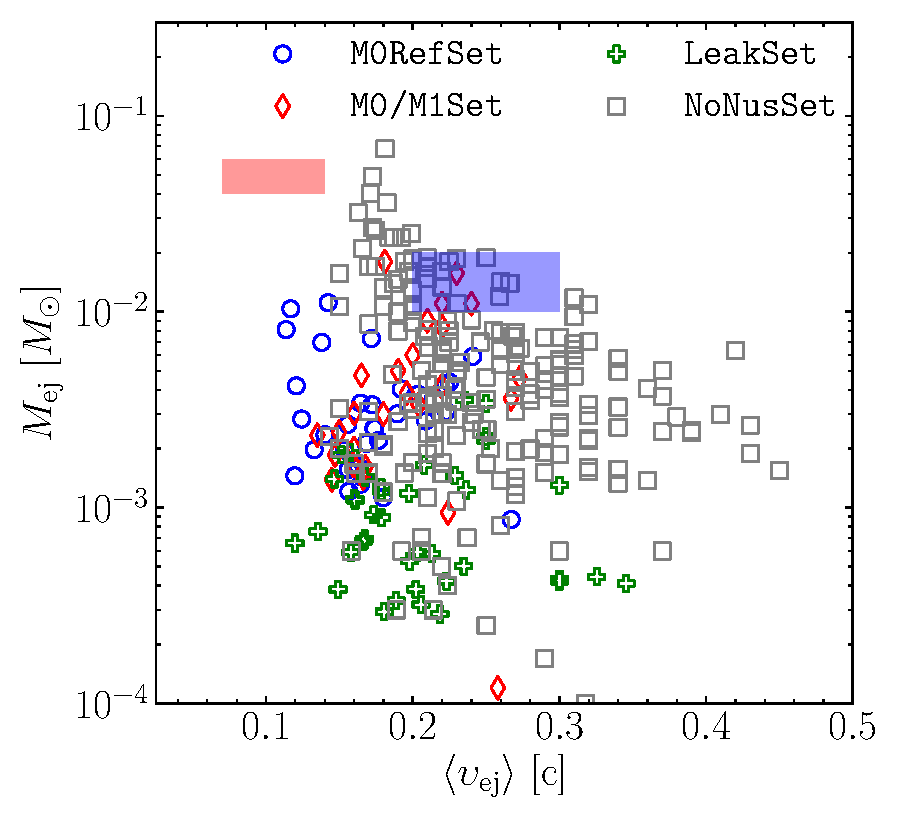
\includegraphics[width=0.45\textwidth]{statistics/ej_mej_vej_groups.pdf}
    \includegraphics[width=0.45\textwidth]{statistics/ej_mej_yeej_groups.pdf}
    \includegraphics[width=0.45\textwidth]{statistics/ej_vej_yeej_groups.pdf}
    \caption{
        Properties of \ac{DE} for all datasets (Tab.~\ref{tab:data}), 
        including total ejecta mass, $M_{\rm ej}$, mass-averaged electron 
        fraction, $\langle Y_{\rm e;ej}$, and velocity 
        $\lambda\upsilon_{\rm ej}\rangle$. 
        The colored patches represent ranges inferred from \AT{} 
        \ac{kN} models \citep{Villar:2017wcc,Siegel:2019mlp}  
        (see Ch.~\ref{ch:kilonova} for the \ac{kN} discussion). 
        (Adapted from \citet{Nedora:2020qtd}). 
%        Summary of dynamical ejecta properties used in this work.
%        Blue circles represent models of \DSrefset{}, 
%        red diamonds stands for models from \DSheatcool{}, 
%        green crosses are models from \DScool{}
%        and gray squares stand for models from \DSnone{}, 
%        We show for comparison the two-component fit to AT2017gfo as
%        colored patches from \cite{Villar:2017wcc,Siegel:2019mlp}.
%        (Adapted from \citet{Nedora:2020qtd})
    }
    \label{fig:ejecta:dyn:ds}
\end{figure*}

The datasets used for the analysis are summarized in Tab.~\ref{tab:data}.
We group them with respect to the employed neutrino treatment:

\begin{itemize}
    %% ---
    \item \DSheatcool{} comprises a set of models with neutrino emission 
    and absorption and microphysical \acp{EOS}. It includes 
    $8$ models with leakage+M0 scheme of \citet{Radice:2018pdn} and models 
    of \citet{Sekiguchi:2015dma,Sekiguchi:2016bjd,Vincent:2019kor},
    in which leakage+M1 scheme or gray M1 scheme are employed for the neutrino transport. 
    Models reported in these studies span 
    $q\in[1, 1.30]$, 
    $\tilde{\Lambda}\in[340, 1437]$, 
    $M_{\rm tot}\in[2.52,2.88]$, 
    and $M_{\rm chirp}\in[1.10,1.25]$.
    %% ---
    \item \DSrefset{} harbors our models. 
    %    with the same physical setup as 
    %    those models with leakage+M0 of \citet{Radice:2018pdn}, that are 
    %    part of the \DSheatcool{}. However, these models, presented in 
    %    \citet{Perego:2019adq,Nedora:2019jhl,Bernuzzi:2020txg,Nedora:2020pak}, 
    %    and disucssed in Ch.~\ref{ch:bns_sims}, 
    Because they are uniform in terms of  
    numerical setup, code and physics, and have fixed chirp mass, 
    we group them into a separate, reference dataset. 
    The models of this set span $q\in[1, 1.82]$, 
    $\tilde{\Lambda}\in[400, 850]$, 
    $M_{\rm tot}\in[2.73,2.88]$ with 
    the chirp mass $M_{\rm chirp}=1.19$.
    %% ---
    \item \DScool{} comprises models with leakage scheme as neutrino treatment and 
    microphysical \acp{EOS}. The dataset includes a subset of models from 
    \citet{Radice:2018pdn} %($35$ runs denoted as LK),
    and the set of models from \citet{Lehner:2016lxy}.
    The models in this dataset span $q\in[1, 1.31]$, 
    $\tilde{\Lambda}\in[116, 1688]$, 
    $M_{\rm tot}\in[2.40,3.42]$, 
    and $M_{\rm chirp}\in[1.04,1.49]$.
    %% ---
    \item \DSnone{} is composed of models with piecewise-polytropic \acp{EOS} 
    of \citet{Hotokezaka:2012ze,Dietrich:2015iva,Dietrich:2016hky,
        Kiuchi:2019lls,Bauswein:2013yna},
    in which temperature effects are approximated by a
    gamma-law pressure contribution, while
    composition and weak effects are neglected.
    The models in this dataset span 
    $q\in[1, 2.06]$, 
    $\tilde{\Lambda}\in[50, 3196]$, 
    $M_{\rm tot}\in[2.4,4.0]$, 
    and $M_{\rm chirp}\in[1.04,1.74]$.
\end{itemize}

%% --- Overal dataseamble
In total $324$ \ac{NR} models are collected. In cases where $\tilde{\Lambda}$ 
is not available, we compute it by solving \ac{TOV} equations\footnote{
    The code for solving \ac{TOV} equations for a \ac{NS} with a tabulated 
    \ac{EOS} was developed by Sebastiano Bernuzzi, a simplified version of which is 
    available at \url{http://sbernuzzi.gitpages.tpi.uni-jena.de/gr/}.
}
for the corresponding gravitational masses and \acp{EOS}.
% 
For a subset of models with polytropic \acp{EOS} of \citet{Bauswein:2013jpa}
and \citet{Kiuchi:2019lls}, however, the \ac{EOS} data are not available and 
the $\tilde{\Lambda}$ cannot be estimated. We exclude these models from the 
statistical analysis. Overall, out of $324$, we consider $271$ models for which 
the required binary data are available/computed. For all $271$ models the ejecta 
mass, $\amd$, is present. The average velocity, $\avd$, is available for only $246$ 
models, as a subset of models from \citet{Kiuchi:2019lls} does not contain this 
information. The electron fraction is found for $99$ models, as we exclude the 
subset of models of \citet{Lehner:2016lxy} with leakage scheme for which these 
data are not given. 
%The \ac{RMS} half-opening angle around the orbital plane, 
%$\athetarms$, of the ejecta is present for $76$ models and the mass of the disk, 
%$M_{\rm disk}$, is given for $119$ models.


The collected data are shown in Fig.~\ref{fig:ejecta:dyn:ds}. We note that the overall properties of \ac{DE} are similar between the \DSrefset{} and \DSheatcool{}. This is expected, as these 
datasets include similar, albeit not the same, physics, regarding \ac{EOS} and neutrino treatment.
%
The important exceptions are the high \mr{} models of \DSrefset{}, 
that undergo \ac{PC}. \ac{DE} ejecta from these models is of tidal origin only. 
%\citep{Bernuzzi:2020txg}.

Comparing the properties of datasets with and without neutrino reabsorption, we observed 
that the the inclusion of this effect leads to an increase in \ac{DE} mass, in addition to the expected increase in average electron fraction. This is especially 
noticeable when comparing models of \DSrefset{} and a subset of 
\citet{Radice:2018pdn} with leakage scheme only.


In Appendix \ref{app:coefs} we report detailed statistical analysis, where we examine the 
change in mean values of ejecta properties between different datasets and fit the 
data with different fitting formulae found in the literature, as well as applying simple 
polynomials of $q$ and $\tilde{\Lambda}$ of second order,
$P_2^1(\tilde{\Lambda})$ and $P_2^2(q,\tilde{\Lambda})$, respectively. 
The results of this analysis are the following. 

%% --- Mej
For the ejecta mass we observe that the inclusion of \mr{} into a fitting formula 
is required to capture the leading trends in data and the simple polynomial, 
$P_2^2(q,\tilde{\Lambda})$, shows a comparatively good statistical performance.
%\gray{We recomment the calibration based on the models with }
%
The statistical analysis also suggests that the $\amd$ depends 
sensibly on the physics input of the simulations: the neutrino scheme and \ac{EOS} treatment.
%
The magnitude of systematic uncertainties in the data, however, reduces the ability of any 
fitting formula to identify and quantitatively capture leading trends.
%

\begin{figure*}[t]
    \centering 
    \includegraphics[width=0.45\textwidth]{statistics/ej_mej_theta_groups.pdf}
    \includegraphics[width=0.45\textwidth]{statistics/ej_vej_theta_groups.pdf}
    \includegraphics[width=0.45\textwidth]{statistics/ej_theta_yeej_groups.pdf}
    \caption{
        Same as Fig.~\ref{fig:ejecta:dyn:ds}, but including also the 
        mass-averaged \ac{RMS} half-opening angle about the orbital plane of the 
        \ac{DE} distribution, $\athetarms$. The plotted 
        data is limited to datasets in which this quantity is available. 
        %
        %The last panel shows a clear correlation between $\theta_{\rm RMS}$ and $\ayd$. 
        (Adapted from \citet{Nedora:2020qtd}).
        %        Properties of \ac{DE} for all datasets (Tab.~\ref{tab:data}), 
        %        including total ejecta mass, $M_{\rm ej}$, mass-averaged electron 
        %        fraction, $\langle Y_{\rm e;ej}$, and velocity 
        %        $\lambda\upsilon_{\rm ej}\rangle$. 
        %        Relations between the ejecta $\theta_{\rm RMS}$ and other parameters of the dynamical
        %        ejecta: mass, $\amd$, velocity, $\avd$, and electron fraction $\ayd$ for models from
        %        \DSrefset{} and \cite{Radice:2018pdn} from \DScool{} and \DSheatcool{}.
        %        Plots show that models with neutrino absorption have
        %        higher $\amd$ and larger $\theta_{\rm RMS}$ as well as 
        %        a clear correlation between $\theta_{\rm RMS}$ and $\ayd$.
        %        (Adapted from \citet{Nedora:2020qtd})
    }
    \label{fig:ejecta:dynej_thetarms}
\end{figure*}


%% --- vej
%We find that in our set of models, there is a correlation of $\avd$ with the 
%tidal parameter $\tilde{\Lambda}$: the higher the $\tilde{\Lambda}$ the lower 
%the $\avd$. This can be understood from the tidal/shocked components of the 
%\ac{DE} (see Sec.~\ref{sec:intro:merg_pmerg}) \red{BROKEN REF?}.
Considering the mass-averaged ejecta velocity, $\avd$, of the \DSrefset{} we 
find that it is in overall agreement with the dataset with neutrino leackage scheme 
of \citet{Radice:2018pdn}, and ranges from $0.11\, c$ to $0.27\, c$. However, while in 
that study there was no apparent correlation observed between the velocity and binary 
parameters, upon visual inspection we find that in models of \DSrefset{} the $\avd$ 
is correlated with $\tilde{\Lambda}$, as shown in Fig~\ref{fig:ejecta:dyn:dsfits}.
This might be attributed to the fact that the \DSrefset{} encompass models with fixed 
chirp mass. 
%
The best fitting formula to the $\avd$, among those considered, is $P_2^2(q,\tilde\Lambda)$, 
which appears to be able to capture the leading trends in the data. 
%For its calibration, the dataset with the most advanced physics is 
%recommended, \DSheatcool{} \& \DSrefset{}.
%
The ejecta velocity shows a strong dependency on the neutrino treatment 
and binary parameters, specifically, \mr{}.

%% --- Yeej 
Considering the average value of the mass-averaged electron fraction, $\ayd$, we find 
that when only models of \DSrefset{} are considered, $\ayd$ varies 
between $0.03$, found in very high \mr{} binaries, that produce cold, low-$Y_e$,
tidal ejecta, and $0.27$ in $q\sim1$  % \citep{Bernuzzi:2020tgt}
binaries, where the contribution from the shocked component is significant 
(see also Fig.~\ref{fig:ejecta:dyn:dsfits}). 
%
Naturally, datasets that include the effects of neutrino absorption display 
on average higher $\ayd$. 
%
Here we only consider the polynomials as fitting formulae. 
The analysis suggests that $P_2^2(q,\tilde\Lambda)$ is the best fitting one, 
as it is able to reproduce both the low-$Y_e$ and high-$Y_e$ models of 
\DSheatcool{} and \DSrefset{}.
%Comparing the values of $\ayd$ from datasets and predicted by fitting formulae in 
%we find that for all datasets, the $P_2^2(q,\tilde\Lambda)$ is able to 
%reproduce both the low-$Y_e$ and high-$Y_e$ models of 
%\DSheatcool{} and \DSrefset{}.

%% --- theta_RMS
%% THETA RMS [3 pandles REFSET]



\begin{figure*}[t!]
    \centering 
    \includegraphics[width=0.49\textwidth]{ejecta_dyn/fast_ejecta/BLh_q100_LK_SR.pdf}
    \includegraphics[width=0.49\textwidth]{ejecta_dyn/fast_ejecta/SFHo_q100_LK_SR.pdf}
    \includegraphics[width=0.49\textwidth]{ejecta_dyn/fast_ejecta/SFHo_q112_LK_SR.pdf}
    %% \includegraphics[width=0.49\textwidth]{./figs/scatter_lambda_ekej_vej06.pdf}
    %% \includegraphics[width=0.49\textwidth]{./figs/scatter_mej_vej06.pdf}
    %% \includegraphics[width=0.49\textwidth]{./figs/scatter_total_kinetic_energy.pdf}
    %%     \includegraphics[width=0.49\textwidth]{./figs/scatter_thetarms_vej06.pdf}
    %%     \includegraphics[width=0.49\textwidth]{figs/scatter_lightcurve_peaks_vs_lambda.pdf}
    \caption{
        Time evolution of the fast tail of \ac{DE}, $\dot{M}(\upsilon_{\rm ej}>0.6\,c)$, 
        alongside the time evolution of normalized central density $n_{\rm max}/n_{\rm nuc}$ 
        for three simulations, BLh $q=1.00$, SFHo $q=1.00$ and SFHo $q=1.13$, one per panel. 
        %
        The lower subpanel on each panel depicts the time evolution of the fast tail of 
        \ac{DE} angular distribution. 
        %% \vn{[Might be removed, if needed]}
        %        Ejection mechanism and properties of the fast tail of the ejecta shown for three simulations,
        %        with two \acp{EOS}: BLh and SFHo and two \mr{}s: $q=1.00$ and $q=1.22$.
        %        %% ---
        %        The upper panel in each plot shows the time evolution of the maximum density 
        %        in the simulation (green curves) and the mass flux of the ejecta with 
        %        asymptotic velocities exceeding $0.6c$ (red curve).
        %        %% --- 
        %        The bottom panel shows the mass histogram of the fast ejecta tail as a function 
        %        of time. 
        %% --- 
        In both panels the outflow rate and histograms are computed at a radius of 
        $R = 443$~km and shifted in time by 
        $R\langle\upsilon_{\rm fast}\rangle ^{-1}$, 
        $\langle\upsilon_{\rm fast}\rangle$ being the mass averaged velocity of 
        the fast tail at the radius $R$.
        %% --- 
        %        The plot shows that while in mist models the peak of the fast ejecta mass flux 
        %        coincides with the first core \bnc{}, in agreement with \cite{Radice:2018pdn}, 
        %        in the model with 
        %        
        %        The plot shows that most of the fast ejecta are generally produced at first core \bnc{} with a contribution from the second in models with soft \acp{EOS}.
        (Adapted from \citet{Nedora:2021eoj}). 
    } 
    \label{fig:ejecta_v06_mech}
\end{figure*}

%
The ejecta geometry has been shown to be very important for modeling \ac{EM} 
counterparts to mergers (see Chapter~\ref{ch:kilonova} and Chapter~\ref{ch:afterglow}). %\citep[\eg][]{Perego:2017wtu}. 
However, its statistical analysis is very non-trivial. 
Because of the limited data, and for the sake of simplicity, 
we consider the mass-averaged \ac{RMS} half-opening 
angle of the ejecta about the plane of the binary, $\athetarms$.
%% --- 
We introduce the $\athetarms$ in accordance with \citet{Radice:2018pdn}, assuming 
the axial symmetry and computing:
%
\begin{equation}
\athetarms = \frac{180}{\pi}\Bigg(\frac{\sum m_i \theta_i^2}{\sum m_i}\Bigg)^{1/2}\, ,
\end{equation}
%
where $\theta_i$ and $m_i$ are the angle (from the binary plane), and the mass of 
an element of \ac{DE}, respectively.
%
Unfortunately, this quantity is available only for the \DSrefset{} and for a subset 
of models of \citet{Radice:2018pdn}. 
% some of which are in \DScool{} and some are in \DSheatcool{} (see Tab~\ref{tab:data}). 
Hence, the statistical analysis is limited 
to a small sample of models. 

The dependency of the $\athetarms$ on other ejecta 
properties discussed above is shown in Fig.~\ref{fig:ejecta:dynej_thetarms}.
%
With respect to the models of \citet{Radice:2018pdn}, we observe that the models of  
\DSrefset{} have overall larger $\athetarms$. This suggests that the inclusion of 
neutrino reabsorption leads to a more spherically distributed ejecta.
%
The third panel of Fig.~\ref{fig:ejecta:dynej_thetarms} shows a clear linear relation 
between the $\athetarms$ and $\ayd$ that can be attributed to the \mr{} dependency of 
\ac{DE} properties observed above, which we extend as follows. 
Binaries with large \mr{}s have ejecta of mostly tidal origin that 
is confined to the binary plane and characterized by a low electron fraction. 
Meanwhile, binaries with $q\sim 1$ have ejecta of both tidal and shocked origin that are both 
more spread out and more processed by shocks and neutrino irradiation having, thus,
higher $\ayd$. 
%
Similar to the case of $\ayd$, we find that the \polql{} provides the best fit to the data.
%
All coefficients to all fitting formulae are reported in Appendix~\ref{ch:stat}. 


Overall, we observe that the properties of \ac{DE} depend on \mr{} and 
\ac{EOS} softness that can be parameterized with $\tilde{\Lambda}$, and a simple 
polynomial in these two quantities show a comparable or better performance with 
resepct to other fitting formulae available in the literature. 
%
However, a larger sample of ab-initio \ac{NR} simulations with complete physics and 
publicly available data is required to refine these relations.

%We overview the overall properties of the dynamical ejecta in our simulations 
%in in the chapter \ref{ch:stat}, placing them alongside the other available data 
%in the literature.

%We can qualitatively asses the effects of neutrino heating by comparing the overall 
%properties of our models with those of \citet{Radice:2018pdn}, where the same 
%simulation setup and code were used but only neutrino leakage scheme was employed.
%%
%We perform this comparison and the comprehansive statitical analysis of the 
%ejecta properties in the chapter \ref{ch:stat}.
%
%Specifically, we observer, 
%Comparing out simulation data with other models available in the literature 
%(Sec.~\ref{sec:stat:ejecta}), we find that neutrino absorption leads to not only 
%an increase in average electron fraction but also to larger total ejected mass 
%and velocity. 
%The latter two would be crucial for the non-thermal, 
%kilonova afterglow (see Sec.\red{sec:KilonovaAfterglow}).
%%
%The mass averaged over the simulations from Tab.~\ref{tab:sim} is 
%$\overline{\amd} = (3.442 \pm 2.495)\times 10^{-3}\,M_{\odot}$ (where
%hereafter we report also the standard deviation), while the same
%quantity calculated for data of \citep{Radice:2018pdn} 
%is $\overline{\md} = (1.352\pm 1.250)\times 10^{-3}\,\Msun$.
%The mass-averaged terminal velocity of the dynamical ejecta 
%ranges between $0.1\,c$ and $0.3\,c$, and in a good agreement with 
%\citep{Radice:2018pdn}.
%The mass-averaged velocity, averaged over all the simulations, is 
%$\overline{\avd} = (0.172\pm0.038)\,{\text{c}}$.
%
%We find that in our set of models, there is a correlation of $\avd$ with the 
%tidal parameter $\tilde{\Lambda}$: the higher the $\tilde{\Lambda}$ the lower 
%the $\avd$. This can be understood from the tidal/shocked components of the 
%\ac{DE} (see Sec.~\ref{sec:intro:merg_pmerg}) \red{BROKEN REF?}.
%%
%We also find that the ejecta velocity, found in our simulations, 
%is recovered in \ac{NR} simulations with more advanced neutrino 
%treatment performed by other groups (see App.~\ref{sec:stat:vejstat}).
%
%From the plot we observe that the $\avd$ increases with $\tilde{\Lambda}$. This can 
%be attributed to the fact that the \ac{DE} in mergers with $q\sim1$ is dominated by the 
%shocked component and that the shocked component has on average higher velocities when 
%the \acp{NS} of lower radii (with larger $\tilde{\Lambda}$) collide.
%
%that tells in mergers of binaries with $q=1.00$, the shocked component of the ejecta 
%is the dominant. The strength of shocks increases as the \acp{NS} become more compact 
%(with decreasing $\tilde{\Lambda}$) and hence collide at higher velocities~\footnote{Note that in the definition of prompt collapse we adopted, there is no shocked ejecta.}.
%%% ---
%For binaries with high mass ration, however, the tidal component of the \ac{DE} is dominant. 
%The velocity of the latter also is smaller for larger $\tilde{\Lambda}$, as stars collide 
%at slower velocities due to their larger radii. 
%%% ---
%In our models, the mass-averaged electron fraction, $\ayd$, 
%lies the range $(0.1, 0.3)$.
%with an averaged value among all models $\overline{\ayd} = 0.175 \pm 0.063$.
%Notably, the \citet{Radice:2018pdn} reported a more narrow range, $(0.1, 0.2)$.
%This is a clear effect of the neutrino absorption included in our models, that elevates 
%the everal electron fraction of the \ac{DE} as it is being irradiated by neutrinos 
%during the merger.
%Notably, the $\ayd$ of our models is close to those obtained with M1 
%scheme of \citet{Sekiguchi:2016bjd} and \citet{Vincent:2019kor}.
%%% ---
%The angular distribution of the \ac{DE} is found to depend 
%on the neutrino treatment. Specifically, the inclusion of 
%neutrino reabsorption leads to a more spherically distributed ejecta
%(see App.~\ref{sec:stat:thetarms}).
%%%%---
%The effect of subgrid turbulence on the dynamical ejecta properties however,
%found rather week and comparable to the effects of finite grid discretization 
%\citep{Bernuzzi:2020txg,Radice:2020ids}.
%
%Overall, we observe that the properties of the \ac{DE} depend on the \mr{} and 
%\ac{EOS} softness that can be parameterized with $\tilde{\Lambda}$, as 
%%
%\begin{align}\label{eq:polyfit2}
%P_2 ^1(\tilde{\Lambda}) &= b_0 + b_1\tilde\Lambda + b_2 \tilde\Lambda^2, \\\label{eq:polyfit22}
%P_2 ^2(q,\tilde\Lambda) &= b_0 + b_1q + b_2\tilde\Lambda + b_3q ^2 +  b_4 q \tilde\Lambda + b_5\tilde\Lambda^2 \, .
%\end{align}
%%
%The result of a fitting ejecta parameters with the polynomial of these two quantities 
%are shown in bottom panels of Fig.~\ref{fig:ejecta:dyn:dsfits}.
%%
%This assertion is supported by a more thorough analysis of the ejecta 
%properties and disk mass, discussed in Appendix.~\ref{ch:stat}, 
%and thus we refer to these formulae as ``best fitting formulae''.
%%
%A larger sample of ab-initio simulations with complete physics and 
%publicly available data are required to refine these relations.






\subsection{Fast tail of dynamical ejecta} \label{sec:bns_sims:fast_de}

%\red{\bnc{} is introduced in intro, Sec.~\ref{sec:intro:merg_pmerg}}

In order to analyze the low mass, very fast component of \ac{DE}, we 
choose the furthest extraction sphere from the remnant, at 
$R = 443\,$km.  %300G/c^2M_{\odot}
%In this section we discuss the ejecta properties that are extracted at 
%coordinate radius of $R=300G/c^2M_{\odot}\approxeq443\,$km from the center.
This ensures that the ejecta had the longest evolution 
within the simulation domain. In addition, this allows for a consistent
comparison with the results of \citet{Radice:2018pdn}.
%
%We also limit the discussion to the simulations performed at a standard resolution
%(ee Sec.~\ref{sec:bns_sims:setup}). Several available simulations that 
%were performed at higher resolution are used to asses the errors.
Following the authors, we define the fast ejecta component (tail) 
as the ejecta with $\upsilon_{\infty}\geq0.6\,c$.

We find a non-negligible amount of fast ejecta in all our simulations 
except for those with very stiff \acp{EOS} and high \mr{}s. 
%We find that not all the simulation show the presence of the fast ejecta tail.
%For instance, the fast ejecta component is absent in simulations with stiff \ac{EOS} 
%and relatively high \mr{}, 
%$q=M_1/M_2\geq1$ where $M_1$ and $M_2$ are the gravitational masses 
%at infinity of the primary and secondary \acp{NS} respectively.
The \ac{DE} velocity distribution from these models shows a sharp cut-off at ${\leq}0.5\,c$ 
that can be attributed to the fact that in these simulations, \ac{DE} 
are primarily of tidal origin and display on average lower velocities, 
that, in turn, are set mainly by \acp{NS} velocities at 
the last orbit and the system escape velocity. 
%The absence of fast tail can be explained by the fact that 
%at large \mr{}s the ejecta are dominated by the tidal component, whose speed 
%is largely set by the \acp{NS} velocities at the last orbit and the system escape velocity.
%Moreover, models with large $q$ in our set undergo prompt collapse 
%with no core bounce \citep{Bernuzzi:2020txg}.

We show the mechanism that is responsible for producing most of the fast ejecta in 
Fig.~\ref{fig:ejecta_v06_mech}. We find that the 
ejection of mass with velocity $\upsilon>0.6\,c$ coincides with core \bnc{}s. 
This was previously noted by \citet{Radice:2018pdn}.
Most of the fast ejecta originate at the first core \bnc{} in 
models with moderately soft \acp{EOS} 
or large \mr{}s, \eg, the BLh $q=1.00$ model. % the equal mass BLh \ac{EOS} model. 
Similar behaviour is observed in models with higher \mr{}s and softer \acp{EOS}. 
%\eg, SFHo \ac{EOS} model.
We also observe that in models with very soft \acp{EOS} 
(and small \mr{}s), \eg, the SLy4* $q=1.00$ model, a strong influx of fast ejecta 
occurs during the second core \bnc{}.
%equal mass SLy4 \ac{EOS} model.
Notably, while the first-\bnc{} component is generally equatorial, 
the second-\bnc{} component is more polar. A possible explanation for this might 
include the increase in baryon pollution of the low latitude region around 
the \pmerg{} remnant.

\begin{figure}%%[t]
    \centering 
    \includegraphics[width=0.50\textwidth]{ejecta_dyn/fast_ejecta/scatter_ekej_vej06.pdf}
    \hspace{-4mm}
    \includegraphics[width=0.50\textwidth]{ejecta_dyn/fast_ejecta/scatter_thetarms_vej06.pdf}
    %% \includegraphics[width=0.49\textwidth]{./figs/scatter_lambda_ekej_vej06.pdf}
    %% \includegraphics[width=0.49\textwidth]{./figs/scatter_mej_vej06.pdf}
    %% \includegraphics[width=0.49\textwidth]{./figs/scatter_total_kinetic_energy.pdf}
    %%     \includegraphics[width=0.49\textwidth]{./figs/scatter_thetarms_vej06.pdf}
    %%     \includegraphics[width=0.49\textwidth]{figs/scatter_lightcurve_peaks_vs_lambda.pdf}
    \caption{
        Total kinetic energy (\textit{left panel}) and \ac{RMS} half-opening angle 
        (\textit{right panel}) as a function of binary \mr{}, $q$, for the 
        of the fast tail of \ac{DE}. 
%        Properties of the fast tail of the dynamical ejecta:
%        total kinetic energy (\textit{top panel}) and 
%        half-\ac{RMS} angle around the binary plane (\textit{bottom panel})
%        from a selected set of simulations where this tail is present (see text).
%        We assume conservative uncertainties for the angle, $0.5$~deg, 
%        and half of the value for the kinetic energy. 
%        The top panel shows that only for some \acp{EOS} the 
%        total kinetic energy appear to depend on mass ration. Specifically, LS220m SFho and SLy4 \acp{EOS}.
%        The half-\ac{RMS} angle appears to depend more on \ac{EOS}, and to be overall larger for high-$q$ models.
        (Adapted from \citet{Nedora:2021eoj}). 
    } 
    \label{fig:ejecta_v06}
\end{figure}

%% --- Paragraph on the resolution effects and error bars 
In our sample of simulations, the resolution does not affect whether there is a fast tail 
of \ac{DE} or not, but it does affect its mass, % $\md(\upsilon>0.6\, c)$. 
and we find that  
%$\md(\upsilon>0.6\, c)$ 
it changes by a factor of a few 
between \texttt{SR} and \texttt{HR} simulations. 
A larger sample of simulations performed at high resolution 
is required to assess this uncertainty more quantitatively.
%% --- Properties of the fast tail: ejecta mass
%The mean value of the fast tail mass is
%\begin{equation}
%    \overline{\amd}(\upsilon>0.6\, c) = (2.36 \pm 3.89)\times 10^{-5}\,M_{\odot}\ ,
%\end{equation}
%where we also report the standard deviation.


%% --- Properties of the fast tail: velocity, electron fraction
Mass-averaged properties of the fast ejecta tail, such as velocity, 
electron fraction and angular distribution appear to be robust with resolution, 
similar to what was observed for \ac{DE} overall (see Tab.~\ref{tab:sim}).
%% --- Table reference 
%We report the properties of fast tail in Tab.~\ref{tab:sims}.
%
We find that the mass-averaged velocity % , 
%$\vd(\upsilon>0.6\,c)$, 
is close to $0.6\,c$,
increasing with the softness of the \ac{EOS}.
%
The mass-averaged electron
%, $\yd(\upsilon>0.6\, c)$ 
is generally above $0.25$, 
indicating that these ejecta were shock-heated and reprocessed by neutrinos. The high 
average electron fraction implies that only weak \rproc{} \nuc{} would 
occur, producing elements up to the $2$nd $r$-process peak \citep{Lippuner:2015gwa} 
(see Sec.~\ref{sec:intro:nucleo} and Chapter~\ref{ch:nucleo}).


%% cp ~/GIT/GitHub/bns_em_analysis/scripts/figs/kinetic_energy_struct_models.pdf ~/GIT/GitHub/phd_thesis/v4/Figures/ejecta_dyn/fast_ejecta/
\begin{figure}[t!]
    \centering 
    \includegraphics[width=0.55\textwidth]{ejecta_dyn/fast_ejecta/kinetic_energy_struct_models.pdf}
    \caption{
        Cumulative kinetic energy distribution (\textit{top panel}) for a set of 
        representative model and its angular dependence 
        for the BLh $q=1.00$ model (\textit{bottom panel}). 
        %
        The green line corresponds to $\upsilon_{\rm ej}=0.6$. 
%        Cumulative kinetic energy distribution for a selected set of models (\textit{top panel}) 
%        and its angular distribution for a BLh $q=1.00$ model (\textit{bottom panel}).
%        %% Also shown as a solid black line is the slow quasi-spherical model of \cite{Mooley:2017enz}.
%        The vertical light green line marks the $\upsilon_{\text{ej}}=0.6$.
%        The top panel shows that equal mass models have a more extend high energy tail,
%        while the bottom panel shows that the angular distribution of the ejecta is not 
%        uniform.
        (Adapted from \citet{Nedora:2021eoj}). 
    } 
    \label{fig:ejecta_vel_hist}
\end{figure}

%% --------------------------------
%% TAB WIND SUMMARY
\begin{sidewaystable}
%\begin{table*}[t]
  \centering
  \captionsetup{width=1.0\linewidth}
  \caption{%
    Summary table of the \swind{} properties of long-lived remnants. The columns contain
    the following information, starting from the left. Equation of
    state, mass-ratio, available resolutions,
    inclusion of subgrid turbulence, time of the
    simulation end, mass of the
    \swind{}, mass-loss rate via \swind, mass-averaged electron fracton, terminal
    velocity and, finally, RMS angle for \swind{}. For these four
    quantities we give the mean value among the resolutions and
    one-sigma deviations. For binaries for which only one
    resolution is present, the error is assumed to be $20\%$ of the value.
    (Adapted from \cite{Nedora:2020pak}).
    }
  \label{tab:spiralwavewind}
  \begin{tabular}{c c c c c c c c c c}
    \hline\hline
    EOS & $q$ & Resolution & GRLES & $t_{\text{end}}$ & $\amw$ & $\amw/\Delta t$ & $\ayw$ & $\avw$ & $\langle \theta_{\text{ej}}^{\text{w}} \rangle$ \\
    &   &   &   & [ms] & $[10^{-2} M_{\odot}]$ & $[M_{\odot}/s]$ &   & $[c]$ &   \\ 
    \hline
    \hline
    BLh & 1.00 & \texttt{SR HR LR} & \cmark & $43.3$ $91.8$ $23.1$ & $0.39^{+0.07} _{-0.07} $ & $0.70^{+0.32} _{-0.32} $ & $0.31^{+0.01} _{-0.01} $ & $0.12^{+0.01} _{-0.01} $ & $27.06^{+2.61} _{-2.61} $ \\
    BLh & 1.00 & \texttt{SR} & \xmark & $ $ $103.2$ $ $ & $1.12^{+0.57} _{-0.57} $ & $1.07^{+0.21} _{-0.21} $ & $0.34^{+0.01} _{-0.01} $ & $0.12^{+0.02} _{-0.02} $ & $15.72^{+2.00} _{-2.00} $ \\
    \hline
    BLh & 1.18 & \texttt{LR} & \cmark & $69.4$ $ $ $ $ & $1.28^{+0.64} _{-0.64} $ & $1.23^{+0.25} _{-0.25} $ & $0.33^{+0.01} _{-0.01} $ & $0.11^{+0.02} _{-0.02} $ & $14.98^{+2.00} _{-2.00} $ \\
    \hline
    BLh & 1.43 & \texttt{LR SR} & \cmark & $35.1$ $59.6$ $ $ & $0.75^{+0.18} _{-0.18} $ & $1.06^{+0.67} _{-0.67} $ & $0.27^{+0.01} _{-0.01} $ & $0.09^{+0.01} _{-0.01} $ & $19.43^{+2.22} _{-2.22} $ \\
    \hline
    BLh & 1.54 & \texttt{LR} & \cmark & $45.8$ $ $ $ $ & $0.63^{+0.32} _{-0.32} $ & $0.44^{+0.09} _{-0.09} $ & $0.32^{+0.01} _{-0.01} $ & $0.10^{+0.02} _{-0.02} $ & $21.46^{+2.00} _{-2.00} $ \\
    \hline
    BLh & 1.66 & \texttt{LR SR} & \cmark & $64.6$ $20.1$ $ $ & $0.12^{+0.09} _{-0.09} $ & $0.37^{+0.34} _{-0.34} $ & $0.33^{+0.05} _{-0.05} $ & $0.13^{+0.01} _{-0.01} $ & $52.08^{+20.89} _{-20.89} $ \\
    \hline
    \hline
    DD2 & 1.00 & \texttt{LR SR HR} & \cmark & $123.0$ $113.0$ $74.4$ & $1.25^{+0.14} _{-0.14} $ & $1.30^{+0.19} _{-0.19} $ & $0.30^{+0.01} _{-0.01} $ & $0.17^{+0.00} _{-0.00} $ & $14.88^{+0.87} _{-0.87} $ \\
    \hline
    DD2 & 1.20 & \texttt{LR SR HR} & \xmark & $37.3$ $91.0$ $55.2$ & $0.48^{+0.09} _{-0.09} $ & $0.74^{+0.24} _{-0.24} $ & $0.26^{+0.01} _{-0.01} $ & $0.15^{+0.00} _{-0.00} $ & $24.54^{+2.23} _{-2.23} $ \\
    \hline
    DD2 & 1.43 & \texttt{LR SR} & \cmark & $37.7$ $62.0$ $ $ & $0.60^{+0.02} _{-0.02} $ & $0.51^{+0.06} _{-0.06} $ & $0.23^{+0.12} _{-0.12} $ & $0.16^{+0.00} _{-0.00} $ & $21.74^{+0.03} _{-0.03} $ \\
    \hline
    \hline
    SFHo & 1.43 & \texttt{SR} & \cmark & $ $ $46.5$ $ $ & $0.58^{+0.30} _{-0.30} $ & $0.43^{+0.09} _{-0.09} $ & $0.31^{+0.01} _{-0.01} $ & $0.17^{+0.02} _{-0.02} $ & $22.67^{+2.00} _{-2.00} $ \\
    \hline
    \hline
    SLy4 & 1.43 & \texttt{SR} & \cmark & $ $ $40.3$ $ $ & $0.53^{+0.27} _{-0.27} $ & $0.38^{+0.08} _{-0.08} $ & $0.29^{+0.01} _{-0.01} $ & $0.18^{+0.02} _{-0.02} $ & $23.52^{+2.00} _{-2.00} $ \\
    \hline\hline
\end{tabular}
%\end{table*}
\end{sidewaystable}

%% --------------------------------

%% --- Total energy discussion :: Fig.1 (top)
The total kinetic energy of the fast tail, $E_{\rm k}(\upsilon > 0.6\, c)$,
is shown in Fig.~\ref{fig:ejecta_v06}, first panel. 
Considering the resolution dependency of the ejecta properties discussed 
above, we set a conservative error bar of ${\sim}1$~order of magnitude.
%
The figure shows that the $E_{\rm k}(\upsilon > 0.6\, c)$ ranges between 
${\sim}10^{46}\,$erg, and ${\geq}10^{50}\,$erg, without clear dependency on 
the \ac{EOS}, even though models with very soft \acp{EOS} 
(\eg, SLy4 and SFHo) tend to display larger energies. 
%
The dependency on the \mr{} is more noticeable, especially for 
SLy4, SFHo and LS220 \acp{EOS}, where for the latter, the 
$E_{\rm k}(\upsilon > 0.6\, c)$ 
increases by ${\sim3}\,$ orders of magnitude between $q=1$ and $q=1.7$. 
%Notably, for the BLh \ac{EOS} models, the $E_{\rm k}(\upsilon > 0.6\, c)$ 
%does not change with the \mr{}.



%% --- Angular distribution :: Fig.1 (bottom)
Considering the \ac{RMS} half-opening angle of the fast ejecta around the 
orbital plane (Fig.~\ref{fig:ejecta_v06}, second panel) we set the conservative 
error of $5$~degrees based on the comparison with higher resolution
simulations. 
%
%The figure allows to gauge which ejection mechanism dominates in 
%various simulation, as the ejecta angular distribution depends on it.
%
We observe that in models with stiff \acp{EOS}, \eg, DD2 \ac{EOS}, where the 
first core-\bnc{} ejection mechanism dominates, the fast ejecta tail is generally equatorial.
Meanwhile, in simulations with soft \acp{EOS} and high \mr{}s, the fast ejecta show 
a more uniform angular distribution set by a combination of the core dynamics and 
finite temperature effects. % driving shocked material.

%%% --- RESOLUTION DEPENDENCY 
%%Comparing the total kinetic energy from simulations performed at standard and high resolutions we find that the $E_{\rm k;\, ej}$, is 
%Assessing the resolution dependency of the ejecta parameters more quantitatively,
%we report that for three representative models 
%%for which the fast ejecta 
%%were found in both the SR and high HR simulations, 
%%% (with typical grid resolution $185$~m and $123$~m respectively) 
%the $E_{\rm k \,; ej}(\upsilon_{\text{ej}} > 0.6)$ changes
%by at least factor of a few
%between \texttt{SR} and \texttt{HR}. 
%The ejecta \ac{RMS} half-opening angle about the 
%orbital plane is changing by utmost ${\sim}50\%$.






%% --- KINETIC ENERGY DISTRIBUTION :: Fig.2 <---> Relevant for afterglow
% Next we consider the ejecta kinetic energy distribution, which is defined as
% $E_k(>\Gamma\beta) \propto \Gamma\beta$, 
% where $E_k = 0.5 \md (c\beta)^2$ is the kinetic energy and 
% $\beta$ is the ejecta velocity, expressed in units of $c$,
% and $\Gamma = 1/\sqrt{1-\beta^2}$ is the Lorentz factor.
% $E_k(>\Gamma\beta) \propto \Gamma\beta $ is shown in Fig.~\ref{fig:ejecta_vel_hist}.
% \alp{Is this definition appropriate here? This looks like, maybe, the total kinetic energy. And why is it proportional to $\Gamma \beta$? What about:}
%
Next we examine the distribution of the cumulative kinetic energy of \ac{DE},
defined as the total kinetic energy of \ac{DE} with velocity exceeding 
a certain value, and denoted as $E_k(>\Gamma\beta)$.
Here $\beta$ is the ejecta velocity expressed in units of $c$ and 
$\Gamma = 1/\sqrt{1-\beta^2}$ is the Lorentz factor.
%
The result is shown in Fig.~\ref{fig:ejecta_vel_hist}. 
%
%For a subset of models the $E_k(>\Gamma\beta)$ is presented in Fig.~\ref{fig:ejecta_vel_hist}. 
%
We observe that for all models the bulk of the kinetic energy is confined to 
the low $\Gamma\beta$ matter.
However, models with soft \acp{EOS}, (\eg, SLy4) and small \mr{}s show an
extended high $\Gamma\beta$ tail.
%% The fast tail of the ejecta there is clearly seen for SLy4 $q=1.00$ model. 
%% High $q$ models however, have more narrow distribution, with BLh $q=1.82$ 

The bottom panel of Fig.~\ref{fig:ejecta_vel_hist} illustrates the 
cumulative kinetic energy distribution in terms of $\Gamma\beta$ and angle 
from the plane of the binary for the 
BLh $q=1.00$ model.
%$q=1.00$ model with BLh \ac{EOS}.
The plot shows that the distribution is not uniform with respect to the angle.
High velocity matter is confined more to the plane of the binary, while
a large fraction of very energetic matter is channeled into the polar region. 
% \alp{This final sentence is not clear to me. Maybe do you mean:
% "The distribution is not uniform with respect to the polar angle since the highly energetic components extends up to the polar region, but the highest $\Gamma\beta$ contribution is confined to an equatorial tail." or something similar?}

%Fig.~\ref{fig:ejecta_vel_hist}. 
%Notably, since the largest part (in mass) of the ejecta is equatorial it eludes the 
%interaction with the \ac{GRB} collimated ejecta and expands into an unshocked \ac{ISM}.
%The latter can decrease the \ac{ISM} density and delay the peak of the 
%synchotron emission \citep{2020MNRAS.495.4981M}.
%\red{move that to afterglow and rephrase}




% \red{To be filled when the Afterglow paper is on arxive}



%It was found that, within the velocity distribution of the \ac{DE}, 
%some simulations contain also a very fast tail with $\upsilon_{\text{ej}}\geq0.6c$ 
%\citep{Piran:2012wd,Hotokezaka:2013b,Kyutoku:2012fv,Metzger:2014yda,Ishii:2018yjg,
%       Hotokezaka:2018gmo,Radice:2018pdn}.
%%
%Analysis of the \ac{NR} \ac{BNS} merger simulations ejecta showed that the 
%parameters of this tail  dependents on the binary \mr{} and \ac{EOS} and
%to some extend, on the simulation resolution. 
%Typical masses of the fast tail found are $\sim 10^{-6}-10^{-5} M_{\odot}$. 
%%
%This fast tail can be decomposed into two components:
%the early, polar fast ejecta that originate at the collisional interface of, mostly, 
%equal mass models with soft \acp{EOS};
%%% that experience violent mergers.
%and the late, equatorial fast ejecta, that are driven by the shock breakout from the 
%ejecta after the first core bounce \citep{Radice:2018pdn}.

%\begin{figure}[t]
%    \centering 
%    \includegraphics[width=0.49\textwidth]{./figs/kinetic_energy_struct_models.pdf}
%    \caption{
%        Total kinetic energy distribution for a selected set of models (\textit{top panel}) 
%        and angular distribution of kinetic energy for a BLh $q=1.00$ model (\textit{bottom panel}).
%        %% Also shown as a solid black line is the slow quasi-spherical model of \cite{Mooley:2017enz}.
%        The vertical light green line marks the $\upsilon_{\text{ej}}=0.6$.
%        The top panel shows that equal mass models have a more extend high energy tail,
%        while the bottom panel shows that the angular distribution of the ejecta is not 
%        uniform.
%        \red{Adopted from Nedora et al. (2021)}
%    } 
%    \label{fig:ejecta_vel_hist}
%\end{figure}
%
%The velocity distribution of \ac{DE} was found to include a very fast, 
%$\upsilon_{\text{ej}}\geq0.6$~c tail
%\cite{Piran:2012wd,Hotokezaka:2013b,Kyutoku:2012fv,Ishii:2018yjg,Hotokezaka:2018gmo,Radice:2018pdn}.
%%% ---
%The total mass of this tail was found to be dependent on the
%binary parameters and solution resolution,
%with an average $\sim 10^{-6}-10^{-5} M_{\odot}$.
%%% ---
%With respect to the fast tail origin, it can be divided into two main components 
%\citep{Radice:2018pdn}.
%The early component, that comprises the ejecta that is generated at the collisional interface 
%of two \acp{NS} of similar mass and directed primarily along the binary axes.
%And the late component that consist of matter that driven by the shock breakout from the ejecta 
%after the core bounce and confined mostly to the binary plane. 
%
%Among the simulations listed in \ref{tab:sim}, we select \red{XX} simulations 
%performed at standard resolution, and for which fast ejecta is found.
%%% ---
%Here we extract ejecta properties at the detector located at 
%$R=300G/c^2M_{\odot}\approxeq443$~km, from the merger, in agreement with \citet{Radice:2018pdn}.
%
%The mean value of the fast tail mass is
%
%\be\label{eq:ejecta:dyn:avg:M}
%\red{ \overline{\amd}(\upsilon>0.6) = (2.50 \pm 4.23)\times 10^{-5}M_{\odot}\ , }
%\ee
%
%where the standard deviation is also reported as an error.


%% ------------------ 
%% Note that the geodesic criterion above neglects the fluid's pressure and might
%% underestimate the ejecta mass. The Bernoulli criterion assumes that the (test
%% fluid) flow is stationary, so that there is a pressure gradient that can
%% further push the ejecta.  We find that both criteria predict dynamical
%% ejecta masses that are practically indistiguishable and well within the numerical uncertainties \citep{Bernuzzi:2020txg} if applied to extraction spheres at large coordinate radii; 
%% differences between the two criteria are instead present if they are applied to
%% matter volumes \citep[cf.][]{Kastaun:2014fna}.



\subsection{Spiral-wave wind} \label{sec:bns_sims:sww}

\begin{figure}[t]
    \centering 
    \includegraphics[width=0.50\textwidth]{ejecta_postdyn/wind_mass_flux.pdf}
    %\includegraphics[width=0.55\textwidth]{ejecta_postdyn/ejecta_profiles_dd2_ls220_long.pdf}
    \caption{
        Time evolution of the cumulative \ac{SWW} mass for a set of 
        simulations with long-lived remnants. 
        Here $t_0$ indicates the moment of merger. The wind 
        calculation starts when \ac{DE} saturates ${\gtrsim}10\,$ms \pmerg{}.
%        \emph{Left panel}:
%        Cumulative mass of the \swind{} from long-lived
%        remnants. The wind persists on timescales of $\mathcal{O}(100)\,$ms with
%        mass fluxes ${\sim}0.33-1.23\,\Msun/s$.
%        Adapted from \citet{Nedora:2020pak}.
%        \emph{Right panel}:
%        Evolution of unbound mass for dynamical ejecta
%        (dashed lines)
%        and \swind{}
%        (solid lines). $t=0$ marks the moment of merger, the vertical
%        line marks the collapse time of the model with LS220 \ac{EOS}.
        Adapted from \citet{Nedora:2019jhl}.
    }
    \label{fig:mej:bern}
\end{figure}

%\begin{figure}[t]
%    \centering 
%    \includegraphics[width=0.70\textwidth]{ejecta_postdyn/ejecta_profiles_dd2_ls220_long.pdf}
%    \caption{Evolution of unbound mass for dynamical ejecta
%        (dashed lines)
%        and \swind{}
%        (solid lines). $t=0$ marks the moment of merger, the vertical
%        line marks the collapse time of the model with LS220 \ac{EOS}.
%        Adapted from \cite{Nedora:2019jhl}.
%    }
%    \label{fig:mej:bern_short_long}
%\end{figure}

\begin{figure*}[t]
    \centering 
    \includegraphics[width=0.99\textwidth]{ejecta_postdyn/wind_hists_shared.pdf}
    \caption{
        Properties of the \ac{SWW} from the set of simulations with long-lived 
        remnants. From left to right, the angular, velocity and electron fraction 
        distributions are shown in a form of mass-histograms. 
%        Mass-averaged histograms of the \swind{} for a selected
%        subset of long-lived remnant. From left to right: ejecta angular
%        distribution, ejecta terminal velocity and electron
%        fraction. Remnants from more asymmetric binaries produce winds
%        with broader angular distribution.
%        The \swind{} from the DD2 EOS remnants has larger velocities
%        then the winds from the softer BLh EOS. The electron fraction
%        peaks at ${\sim}0.3$ and it is distributed from $0.1$ to $0.4$.
        (Adapted from \citet{Nedora:2020pak}).
    }
    \label{fig:ejecta:bern:hist}
\end{figure*}

%\begin{figure}[t]
%    \centering
%    %% \includegraphics[width=0.49\textwidth]{ejecta_postdyn/ejecta_profiles_dd2_ls220_long.pdf}
%    %% \includegraphics[width=0.49\textwidth]{ejecta_postdyn/hist_1D_dd2_ls220_long.pdf}
%    \includegraphics[width=0.75\textwidth]{ejecta_postdyn/corr_dd2.pdf}
%    \caption{Properties of the \ac{SWW} and dynamical ejecta
%        computed form the simulations with turbulent viscosity.
%        %
%        Top: evolution of unbound mass for dynamical ejecta
%        (dashed lines)
%        and \ac{SWW}
%        (solid lines). $t=0$ marks the moment of merger, the vertical
%        line marks the collapse time of the LS220 BNS.
%        %
%        Middle: mass histograms for the angular (left), velocity (center) and electron
%        fraction (right) distributions.
%        Bottom: angular distribution and composition of the \ac{SWW}
%        for DD2.
%        %
%        Note the $\bar{M}_{ej}$ in the middle and bottom panels is normalized to one.
%        (Adapted from \citet{Nedora:2019jhl})
%    }
%    \label{fig:ej_properties}
%    
%\end{figure}



As we discussed in the previous section, the interaction between the \ac{NS} remnant 
and the disk generates density waves that propagate outwards through the disk and 
induce massive outflows, \ac{SWW} (see Sec.~\ref{sec:bns_sims:remdisk}).
%
We track \ac{SWW} as the matter unbound according to the Bernoulli criterion 
%$hu_t < -1$, with $h$ being the fluid enthalpy and $u_{\alpha}$ its four-velocity,
(see Sec.~\ref{sec:bns_sims:method:ejecta}), starting after \ac{DE} mass flux 
has saturated (\eg, ${\gtrsim}10\,$ms \pmerg{}), and using the extraction sphere 
located at $R=294\,$km.
%
%The ejecta calculation is turned on when
%the \ac{DE} mass flux stops, which on average corresponds to ${\sim10}$~ms \pmerg{} 
%

%\subsubsection{Spiral wave wind and the remnant lifetime}

%

%We start by considering two representative models, 
%DD2 $q=1.00$ (\texttt{SR}) and LS220 $q=1.00$ (\texttt{SR}), that produce 
%long- and short-loved remnants respectively, 
%We find that if the remnant is long-lived, total \ac{SWW} mass exceeds that of 
%the \ac{DE}. %  as shown also in Fig.~\ref{fig:mej:bern}.
%
%First we consider two representative models that produce long- and short-lived
%remnants. Simulations have $q=1.00$ and DD2 and LS220 \acp{EOS} respectively.
%We find that if the remnant is long-lived, total \ac{SWW} mass exceeds that of the \ac{DE},
%as shown also in Fig.~\ref{fig:mej:bern_short_long}.
%
%This is a simple consequence of the fact the \ac{SWW} mass flux continues for as long as 
%remnant survives.
%
%The inclusion of turbulent viscosity alters all the ejecta masses with an
%additional component \citep{Radice:2018ghv} and, we observe that, it enhances the 
%\ac{SWW} mass by ${\sim}25$\% in the case of DD2 $q=1.00$ model,
%exceeding the finite resolution effects. 
%%\red{Letter stuff. Not sure if true}
%%ac factor that exceeds the resolution effects.
%%
%The latter are ${\sim}15\%$ and ${\sim}8\%$ for the \ac{SWW} mass when the 
%resolution increases from \texttt{SR} to \texttt{HR}.
%The resolution effects on other wind properties, \eg, velocity and $Y_e$, 
%is found to be within $4\%$.
%
%Specifically, we find that the \ac{SWW} mass increases by ${\sim}+15\%$ and
% ${\sim}+8\%$, 
%when the resoltuion increases from LR to SR and from SR to HR respectively.
%Hence, finite grid effects tend to increase mass. A similar analysis on the average 
%electron fraction and velocity indicate variations below $4\%$.
% --- Repetition below
%The angular distribution of the \ac{SWW} resembles that of the \ac{DE} and is 
%largely equatorial, as shown in Fig.~\ref{fig:ej_properties}. 
%%
%The velocity distribution,
%however, is rather different with a narrow peak around $0.1-0.2\,$c, depending on the 
%stiffness of the \ac{EOS}. Notably, properties of the \ac{SWW} are sensitive to the 
%lifetime of the remnant, as at early times they are modified by the trace presence of the 
%\ac{DE} and not-yet-relaxed \pmerg{} environment.
%%
%The electron fraction of the \ac{SWW} also shows a narrow distribution with a peak 
%at ${\geq}0.25$, which is considerably higher than that of the \ac{DE}. 
%Notably, the electron fraction is lower if the remnant is short-lived as it 
%disks around NS remnants are less compact, colder, and optically thicker than those 
%around black holes~\citep{Perego:2019adq}, the outer layers of the DD2 disk have a
%lower $Y_e$ than the LS220 disk and so does the \ac{SWW} coming from those layers.

%\gray{
%    %% From Letter
%    The \ac{SWW} has an angular distribution of mass similar to the
%    dynamical ejecta with material mostly confined to the orbital plane,
%    as shown by the histograms in Fig.~\ref{fig:ej_properties}.
%    On the contrary, the velocity profiles show a drastic difference
%    between the two ejecta components. While the dynamical ejecta has a
%    broad velocity distribution \citep{Hotokezaka:2012ze,Bauswein:2013yna,Radice:2018pdn}, the 
%    \ac{SWW} velocity is narrowly distributed around  
%    $0.2$c in the case of a long-lived remnant (DD2).
%    The \ac{SWW} from the short-lived
%    remnant (LS220) has a broader velocity distribution extending down to
%    $0.1$c.
%    This is due to the spiral-wave shutting down and the disk
%    transition to a more steady accretion. As a consequence, the \ac{SWW}
%    ceases but ejecta continue as a slower disc wind driven
%    by nuclear recombination solely.
%    The electron fraction of the \ac{SWW} has a
%    narrower distribution than the dynamical ejecta in both
%    cases. But because disks around NS remnants are less compact, 
%    colder, and optically thicker than those around black
%    holes~\citep{Perego:2019adq}, the outer layers of the DD2 disk have a 
%    lower $Y_e$ than the LS220 disk and so does the \ac{SWW} coming from
%    those layers.
%    While the \ac{SWW} is generic in its hydrodynamics origin, the
%    quantification of its properties relies on the accurate microphysics and
%    neutrino treatment in our simulations.
%}

% \subsubsection{Spiral wave wind for all models}

In Tab.~\ref{tab:spiralwavewind} we report the overall properties of \ac{SWW} for all models with 
long-lived \ac{NS} remnants that were also evolved for a sufficiently long time. 
%
Notably, in all simulations, \ac{SWW} persist until the 
time these simulations were terminated without saturation. 
%
This is the manifestation of the mechanism driving the outflow: the 
angular momentum and mass transport induced by the dynamical instabilities in the 
remnant, the $m=1,2$ modes. And, as the $m=1$ modes are not efficiently damped \citep{Paschalidis:2015mla,Radice:2016gym,Lehner:2016wjg,East:2016zvv},
\ac{SWW} could theoretically continue until the system collapses to a \ac{BH} 
or reaches an equilibrium. % (Sec.~\ref{sec:bns_dynsmics_overview}).

The time evolution of the cumulative mass of \ac{SWW} is shown in Fig.~\ref{fig:mej:bern}. 
%
The strongest \ac{SWW} are found in binaries with $q>1$, such as the
BLh $q=1.43$ (\texttt{SR}) model. 
With the mass-loss rate ${\sim}0.5\, \Msun/{\text{s}}$ these models can eject 
${\sim}0.02\,\Msun$ within ${\sim}50\,$ms of the \pmerg{} evolution.
%
Meanwhile, models with softer \acp{EOS} reach similarly high mass flux 
at lower \mr{}s. For instance, the mass flux of the BLh* $q=1.66$ model 
is achieved by the LS220* $q=1.22$ model. 
A possible explanation for this is that the softer the \ac{EOS} is, the stronger 
are the $m=1$ modes in the remnant (see Sec.~\ref{sec:bns_sims:remdisk}).

We observe that the inclusion of turbulent viscosity enhances the \ac{SWW} mass 
by ${\sim}25$\% in the case of the DD2 $q=1.00$ model, exceeding the finite 
resolution effects 
%
%The inclusion of turbulent viscosity alters all ejecta masses with an
%additional component \citep{Radice:2018ghv} and, we observe that, it enhances the 
%\ac{SWW} mass by ${\sim}25$\% in the case of DD2 $q=1.00$ model,
%exceeding the finite resolution effects. 
%\red{Letter stuff. Not sure if true}
%ac factor that exceeds the resolution effects.
%
which are ${\sim}15\%$ and ${\sim}8\%$ for the \ac{SWW} mass when the 
resolution increases from \texttt{SR} to \texttt{HR}.
The resolution effects on other wind properties, \eg, velocity and $Y_e$, 
are found to be within $4\%$.

When a \ac{NS} remnant collapses to a \ac{BH} and the mechanism that injects angular 
momentum into the disk shuts down, the \ac{SWW} mass flux subsides.
% (right panel of  Fig.~\ref{fig:mej:bern}). 
Thus, the total ejected mass via \ac{SWW} is directly related to the lifetime of the 
\ac{NS} remnant, in addition to the binary parameters and the \ac{EOS}.

The \ac{SWW} mass flux depends on the disk configuration, as more extended disks 
have outer layers that are less gravitationally bound. In turn, the disk 
configuration is dependent on thermal effects. Higher temperatures lead to 
a stronger thermal pressure that increases the disk size. 
However, the dependency of the \ac{SWW} mass flux on the stiffness of an \ac{EOS} 
appears to be stronger, as stiffer \acp{EOS} lead to more massive disks, 
as discussed in Sec.~\ref{sec:bns_sims:remdisk}.    % contradiction with [1]
%(Fig.~\ref{fig:disk_mass_evo}). 
More simulations with longer \pmerg{} evolution are needed 
to make a quantitative assessment. 
%Overall the \swind{} from the long-lived remnant has a mass flux $\geq 0.4\, \Msun/{\text{s}}$.

%TODO cd ~; cp ~/Tullio/prj_gw170817/BLh_M13641364_M0_LK_SR/{slice_xz_ye_hu_1.pdf,slice_xz_abs_energy_hu_3.pdf,slice_xy_ye_hu_1.pdf,slice_xy_abs_energy_hu_3.pdf} ~/GIT/GitHub/phd_thesis/v4/Figures/slices/
\begin{figure*}[t]
    \centering 
    \includegraphics[width=0.49\textwidth]{slices/slice_xz_ye_hu_1.pdf}
    \hspace{-5mm}
    \includegraphics[width=0.49\textwidth]{slices/slice_xz_abs_energy_hu_3.pdf}
    \includegraphics[width=0.49\textwidth]{slices/slice_xy_ye_hu_1.pdf}
    \hspace{-5mm}
    \includegraphics[width=0.49\textwidth]{slices/slice_xy_abs_energy_hu_3.pdf}
    \caption{
        Snapshots of the BLh $q=1.00$ model taken $88\,$ms \pmerg{}, 
        showing the distribution of electron fraction, $Y_e$, 
        Bernoulli parameter, $-hu_t$, and electron anti-neutron 
        absorption energy rate, $Q_{\text{abs};\:\bar{\nu}_e}$ 
        normalized to the fluid density $D$ in units of $c^{5}/(G M_{\odot})$. 
        \textit{Top row of panels} displays these properties in $(x,z)$ plane, 
        while the \textit{bottom row} shows $(x,y)$ slices. 
%        Snapshots of the BLh $q=1.00$ model taken $88\,$ms \pmerg{}, 
%        displaying the distribution of the electron fraction, $Y_e$, 
%        (\textit{left side of each panel of the right column of panels}), 
%        Bernoulli parameter, $-hu_t$,
%        Snapshot of the $(x,z)$ and $(x,y)$ slices of the BLh $q=1$ model at 
%        ${\sim}89\,$ms after merger. Left panels: electron fraction and
%        $-hu_0$. High $Y_e$ values indicate neutrino
%        postprocessing and irradiation. The $-hu_0>1$ indicates the
%        material that gains enough energy to become unbound at
%        infinity. 
%        %
%        Right: $-hu_0$ and the absorption energy rate $Q_{\text{abs};\:\bar{\nu}_e}$ 
%        of electron antineutrinos normalized to the fluid density $D$.
        %
        (Adapted from \citet{Nedora:2020pak}).
    }
    %
    \label{fig:slice:heating_hu}
\end{figure*}

We find that contrary to the mass flux, other properties of \ac{SWW} 
depend only weakly on the binary parameters and the \ac{EOS}. 
Mass-histograms of the wind angular distribution, velocity and 
electron fraction are displayed in Fig.~\ref{fig:ejecta:bern:hist} 
for several representative models. 
%
The angular distribution of \ac{SWW} is similar to that of \ac{DE}, displaying a 
broad distribution around the binary plane.

\ac{SWW} have a high average electron fraction. Its overall broad distribution,  
$0.1\lesssim \ayw \lesssim0.4$, peaks at ${\simeq}0.35$.
The low electron fraction material originates primarily during early times, when the 
material does not have enough time to be processed by neutrinos and before the 
outflow reaches quasi-steady state.
The \ac{SWW} average velocity is higher in models with stiffer \acp{EOS}, with the peak 
of the distribution lying between ${\sim}0.1\,$c and ${\sim}0.2\,$c.
However, more simulations of the \pmerg{} remnant long-term evolution are 
required to confirm and quantitatively investigate these trends. 
%However, if it is indeed a generic feature, then it might imply 
%an \ac{EOS} dependent distinct feature in the electromagnetic counterpart. 
%In particular, the observation of a fast blue kN given by the \swind{}
%should be associated to a stiff \ac{EOS}.

%% It is however expected, that as the system becomes more stationary and larger part 
%% of the disk accrets on the \ac{MNS} the outflow should subside. 


\subsection{Neutrino-driven wind} \label{sec:bns_sims:nwind}



%In this section we focus on the high electron fraction, polar component of the 
%\acp{SWW}. 

In Sec.~\ref{sec:intro:ejecta} we discussed that, 
the presence of strong neutrino fluxes may drive the emergence of baryonic winds. 
% In Sec.~\ref{sec:intro:ejecta} we discussed that, in the presence of strong 
% neutrino fluxes, baryonic winds may emerge being driven by these neutrino fluxes.  
Since the strongest source of neutrinos is a \ac{NS} remnant, such \nwind{} are 
expected to be polar and characterized by elevated electron fraction 
\citep[\eg][]{Perego:2014fma}. 
%
Having neutrino absorption included in our simulation setup (See 
Sec.~\ref{sec:nr_methods:neut}), we assess whether there are \nwind{} in our 
simulations. Naturally, we expect them to be a part 
of \ac{SWW}, but polar and with high $Y_e$. 
%
For this analysis, for the sake of brevity, we focus on one 
simulation, BLh $q=1.00$ (\texttt{SR}). 


%
In the left column of plots in Fig.~\ref{fig:slice:heating_hu} we compare 
the Bernoulli parameter, $-hu_t$, 
%(see Sec.\ref{sec:bns_sims:method:ejecta}),
and the fluid electron fraction. 
%
In the right column of the plots in Fig.~\ref{fig:slice:heating_hu} we compare 
the Bernoulli parameter with the heating energy rate due to electron anti-neutrino absorption, 
$Q_{\text{abs};\:\bar{\nu}_e}$, computed by the M0 scheme 
(see Sec.~\ref{sec:nr_methods:neut}) and 
normalized with the fluid's conserved rest-mass density.
% and divided by $D=W\rho\sqrt{\gamma}$ 
%(fluid's conserved rest-mass density).
We observe that the electron fraction in the polar region  
($\theta>60^{\circ}$, where $\theta$ is the angle from the binary plane) 
reaches $Y_e\sim0.35$ due to the absorption of 
electron-type anti-neutrinos.
The strongest neutrino heating occurs in the vicinity of the remnant, at densities 
$\rho\sim10^{11}$~\gcm{}, roughly corresponding 
to the location of the neutrinosphere \citep{Endrizzi:2019trv}, 
the region where neutrinos decouple from matter.
%
% to the region where neutrinos decouple,
%the so-called neutrinosphere \citep{Endrizzi:2019trv}.
%
%In Fig.~\ref{fig:slice:heating_hu} we also compare the Bernoulli parameter, 
%$-hu_t$ (see Sec.\ref{sec:bns_sims:method:ejecta}), 
%that is always plotted 
%on the right half of a panel, with the electron fraction (left 
%column of plots and heating energy rate due to electron anti-neutrino absorption 
%$Q_{\text{abs};\:\bar{\nu}_e}$ divided by with $D=W\rho\sqrt{\gamma}$ 
%(fluid's conserved rest-mass density).
%The observed correlation between the $E_\nu/D$ \red{???} and $-h u_t$ further suggests, 
%that the outflow around the polar axis is driven by the neutrino absorption. 
Additionally, we found that if the neutrino absorption is not included into a 
simulation, \eg, using the leakage scheme only, \nwind{} are significantly suppressed.  %\red{bullshit}
%
%The collimated polar outflow can be further boosted and stabilized by the presence of the 
%strong magnetic fields \citep{Bucciantini:2011kx,Ciolfi:2020hgg,Mosta:2020hlh}.

Notably, there is no clear distinction between \nwind{} and \ac{SWW}, especially 
at intermediate latitudes ($\theta \sim 45^{\circ}$), where both strong neutrino fluxes 
and spiral density waves are present. 
%, and both, neutrino absorption and dyanmical effects 
%driving the \ac{SWW} are contributing. 
%
In order to compute the mass flux of \nwind{} we impose additional criteria.
%to the Bernoulli, criteria.
We consider two physically motivated options, the geometrical, flagging the part of 
\ac{SWW} as \nwind{} if they are polar, \ie, $\theta>60^{\circ}$, and the 
composition criterion, \ie, if $Y_e > 0.35$.

We find that \nwind{} are not steady state outflows, contrary to the 
bulk of \ac{SWW}. After the initial strong rise, the mass flux rapidly 
decays in time, and for most models, stops before the simulation is terminated. 
%
This behaviour is independent of the criterion we use. We attribute this to the 
rise of the baryon loading above the remnant as the material gets lifted 
by the thermal pressure from the disk.

The total mass of \nwind{} is ${\sim}10^{-3}-10^{-4}M_{\odot}$. Its 
properties resemble those reported in \eg, 
\citet{Dessart:2008zd,Perego:2014fma,Fujibayashi:2020dvr}.
Notably, in some of the works, \nwind{} were found to require longer 
timescales to develop. %, achieving the quasi-steady state. 
This can be attributed to the strict criteria to isolate the \nwind{} and by 
the absence of \ac{SWW} in other works. 
Additionally, our simulations might not be sufficiently long to achieve the 
conditions required for the development of the quasi-steady state \nwind{}.
%% Additionally, as our models are at most $\sim100$~ms long, the conditions required for the steady 
%% state \nwind{} might not been achieved.



%% =======================================================
%%
%%                   Disc structure
%%
%% =======================================================




%\red{Paragraph on the secular ejecta has been moved to 
%    GW170817 application}

%% =======================================================
%%
%%                   Conclusion
%%
%% =======================================================




%% ========================================================================================

%\section{Statistics of the \ac{DE} parameters and disk mass}
%
%\red{CONTENT OF THE FIT PAPER}
%
%
%\section{Application to \GW{}}
%
%
%\begin{figure*}[t]
%    \centering 
%    \includegraphics[width=0.48\textwidth]{ejecta_dyn/summary/ej_mej_vej_our2.pdf}
%    \includegraphics[width=0.48\textwidth]{ejecta_dyn/summary/ej_mej_yeej_our2.pdf}
%    \caption{
%        Summary of the ejecta properties of our models.
%        %
%        Diamonds mark the dynamical ejecta, crosses include the
%        contribution of the \swind{} for the long-lived models, 
%        triangles are an estimate of the total ejecta mass on a secular
%        timescale, assuming $40\%$ of the disk mass is unbounded on
%        secular timescales.         
%        The ejecta mass is shown is terms of the mass-averaged velocity
%        (left) and of the averaged electron fraction (right).
%        %
%        The filled blue and red patches are the expected values of
%        ejecta mass and velocity for blue and red components of
%        AT2017gfo compiled by \cite{Siegel:2019mlp}, based on
%        \cite{Villar:2017wcc}. 
%        Adopted from \citet{Nedora:2020pak}.
%    }
%    %
%    \label{fig:ejecta:dyn:ds_sww}
%\end{figure*}
%
%
%%% from main paper, referencing the fitpaper Poly22 fits and SWW + DE
%\red{THis can be augmented with Radio afterglow}
%
%%% === FROM DYNAMICAL EJECTA SECTION of MAIN PAPER
%Here we discuss the application of our results to \GW{}.
%
%
%\subsection{Dynamical Ejecta}
%
%
%%% ---
%First, we asses the ejecta parameters that our fitting models, 
%obtained in section \ref{sec:ejecta_disk_statisitcs} would provide for the \GW{}.
%%% --- 
%Considering the $90\%$ credible intervals estimated for $q$ and $\tilde{\Lambda}$ 
%from LIGO-Virgo GW analysis
%\citep{TheLIGOScientific:2017qsa,Abbott:2018wiz,De:2018uhw,Abbott:2018exr},
%i.e.~$\tilde{\Lambda}=300_{-190}^{+500}$ and $q\in[1., 1.37]$. 
%and using the errorbars formulas developed in \cite{Radice:2018pdn}, we find that
%$\amd \in [0.72, 7.52] \times 10^{-3}\: M_{\odot}$
%and
%$\avd \in [0.16, 0.39]$c 
%and 
%$\ayd \in [0.11, 0.23]$.
%Notably, these values do not agree with those inferred for \AT{} by the spherical, 
%two-component kilonova models \citep{Villar:2017wcc}.
%Analysis of a compiled set of kilonova fitting models provides a broad range of ejecta 
%parameters \citep{Siegel:2019mlp}:
%$M_{\text{ej}}^{\text{red}}\in(4, 6)\times10^{-2}M_{\odot}$ and
%$\upsilon_{\text{ej}}^{\text{red}}\in(0.07, 0.14)$ for the red component, while
%$M_{\text{ej}}^{\text{blue}}\in[1, 2]\times10^{-2}M_{\odot}$ and 
%$\upsilon_{\text{ej}}^{\text{blue}}\in[0.2, 0.3]$ for the blue component.
%%% ---
%With respect to our results for \ac{DE}, however, 
%none of the kilonova components can be well explained.
%%% ---
%In Fig.~\ref{fig:ejecta:dyn:ds_sww} we show the ejecta properties from
%all our models (diamonds) and the parameters inferred from the
%observations as red and blue boxes. 
%%% --- 
%With respect to the red component, we observe that \ac{DE} from our models 
%have too high average velocities and not nearly enough mass.
%This result suggests that an additional, low $Y_e$ ejecta component is required
%in order to explain the \AT{} red component 
%\citep{Perego:2017wtu,Kawaguchi:2018ptg,Nedora:2019jhl}.
%%% --- 
%A more thorough analysis of the \AT{} with better ejecta models and advanced
%radiation transport kilonova simulations are not part of the present work 
%and will be addressed in the future.
%
%
%\subsection{Spiral-wave wind}
%
%
%The \ac{SWW} could be a significant contributor to the \AT{}, assuming the remnant of 
%\GW{} \ac{MNS} merger survived for $\mathcal{O}(100)$~ms.
%%% ---- 
%In Fig.~\ref{fig:ejecta:dyn:ds_sww} we report the total
%(dynamical+\swind{}) ejecta mass and mass-averaged velocity for the
%simulated long-lived BNS (crosses).
%%% ---
%Notably, the total ejecta mass of three of our models, 
%BLh $q=1.18$, BLh $q=1.42$ and  DD2 is $q=1$ are in agreemnt with the epected values 
%for the blue compoent of the \AT{} 
%(obtained using the two-component fit \citep{Villar:2017wcc})
%
%\red{
%    [ LETTER STUFF COULD GO HERE ]
%    a multi-component fitting model that explicitly accounts
%    for the \swind{} can fit the early blue
%    emission from AT2017gfo \citep{Nedora:2019jhl}
%}
%
%The high electron fraction of the \ac{SWW} however would result in a lanthanides-poor
%composition of the outflow. Thus, the \ac{SWW} cannot explain the observed emission 
%for the high opacity, lanthanides-rich material.
%%% ---
%Simulations with advanced physics of a \ac{MNS} mergers on a timescales $>100$~ms are 
%required to asses the contribution from other outflow mechanisms, \red{that we will discuss below} 
%\citep{Lee:2009uc,Fernandez:2015use,Siegel:2017nub,Fujibayashi:2017puw,Fernandez:2018kax,Radice:2018xqa}.
%
%
%\subsection{Secular Ejecta}
%
%
%On the timescale of seconds, much longer than the evolution of 
%presented here simulations, the nuclear recombination can unbind 
%a fraction of the disk mass. 
%Analytical estimates and simulations with various approximations show that up tp ${\sim}40\%$ of the disk can be ejected via viscous processes with an typical velocity ${\lesssim}0.1\,$c
%\citep{Lee:2009uc,Fernandez:2015use,Wu:2016pnw,Siegel:2017nub,Fujibayashi:2017puw,Fernandez:2018kax,Radice:2018xqa,Fujibayashi:2020dvr}.
%
%Adapting the fix fraction of the $40\%$ of the disk mass, we estimate 
%that about  ${\sim}0.05\, M_{\odot}$ would be ejected in a form of 
%secular winds. We include this estimate for every simulation
%with the long-lived \ac{MNS} remnant in Fig.~\ref{fig:ejecta:dyn:ds_sww} (lower triangles).
%The estimated mass is sufficient to explain
%the red component of AT2017gfo, as inferred from the two-components kN
%models of \cite{Villar:2017wcc}. 
%
%
%
%
%
%
%
%%% ---------------------
%Sources with time delay are preferred by studies of very metal poor stars that indluded the time delay for r-process elements
%to diffuse through ISM, \citep{Tarumi:2021xvw}. 
%A winds from proto-nuetron are also contributors to the $r$-process budget \cite{Vincenzo:2021rvw}
%
%\red{The remnant is losing anular momentum while disk gains on shortly after merger is due to gravitational torque \cite{Shibata:2019wef}}

% Chapter Template

\chapter{Nucleosynthesis} \label{ch:nucleo}% Main chapter title

%% =======================================================
%%
%%                   Nucleosynthesis
%%
%% =======================================================

%\textcolor{red}{Based on the Jones Lippuner PhD thesis}

%For a long time the general consensus was that all elements in the universe 
%were synthesized during the Big Bang \citep{Alpher:1948}. Later studies have, however, 
%proven that only elements with atomic number $A<8$ were produced 
%(see \eg, \citet{Alpher:1950,Shaviv:2012}). Thus, only the lightest elements, hydrogen 
%and helium primarily, were produced during in the Big Band \citep{Burbidge:1957}. 
%Heavier elements are synthesized in a plethora of processes that we briefly recall here.

%In this chapter we discuss \nuc{} that occurs in the matter ejected in \ac{BNS}
%mergers, focusing on the rapid neutron capture process (\rproc{}) responsible 
%for the creation of heavy elements \citep{Burbidge:1957}. 
%
In Sec.~\ref{sec:intro:nucleo} we discussed the conditions for, and sites of,
\rproc{} \nuc{}, and its contribution to the Universe's chemical evolution. 
%
In this chapter we expand upon this discussion by computing the 
nucleosynthetic yields in ejecta from our \ac{BNS} merger models and 
comparing the result with solar abundances.
%
In Sec.~\ref{sec:nucleo:method} we briefly overview methods for computing  
\rproc{} \nuc{} in merger ejecta, focusing on 
a recently developed nuclear reaction network \texttt{SkyNet} 
\citep{Lippuner:2017tyn,Lippuner:2018phd} and how 
the final nucleosynthetic yields can be parameterized for quick 
estimation of final abundances in \ac{BNS} merger ejecta.
%
In Sec.~\ref{sec:nucleo:results} we present our results.

%In this Chapter we discuss the outcome of the \rproc{} \nuc{} that occurs in 
%matter ejected in our \ac{BNS} merger simulations. 
%We begin by giving a brief overview of how \rproc{} \nuc{} can be modeled, 
%in Sec.~\ref{sec:nucleo:method}, 
%focusing on a recently developed nuclear reaction network \texttt{SkyNet} 
%\citet{Lippuner:2017tyn,Lippuner:2018phd}. Then, we discuss how 
%the final nucleosynthetic yields can be parameterized for quick 
%estimation of final abundances in \ac{BNS} merger ejecta.
%%
%In Sec.~\ref{sec:nucleo:results} we discuss our \ac{BNS} mergers, 
%presented in Chapter~\ref{ch:bns_sims}, computing nucleosynthetic yields 
%and discussing, whether \ac{BNS} mergers can be the main source of \rproc{} 
%elements in the Universe. 

%\red{
%[Lippuner 221 page] Note that luminosity of the electron anti-neutrino is higher then the one of the 
%electron neutrino due to \magenta{re-leptonization} of the neutrino emitting disk \cite{Foucart:2015gaa}.
%}

%\section{Heaviest elements in the Universe}
%\label{sec:nuc:rproc}




%% =======================================================
%%
%%                   Nucleosynthesis SkyNET
%%
%% =======================================================

\section{Modeling the nucleosynthesis}\label{sec:nucleo:method}

%Nuclear reactions play an important role in numerous astrophysical cites, 
%where sufficiently high temperatures and densities are achieved. 
%In particular, in main sequence stars nuclear fusion prevents stars from collapsing, releasing the binding energy, 
%counteracting gravity \citep{Bethe:1939}. When stars do undergo a core collapse, the nuclear and weak reactions 
%govern the explosion by introducing and removing energy (\eg, via neutrino cooling and heating). 
%%
%A small amount of the material synthesized in the explosive burning is ejected into the \ac{ISM}  
%\citep{Nomoto:1997if,Woosley:2002}. It is composed mostly of iron-group elements, enriched with heavier elements 
%synthesized in weak \rproc{} \citep{Wanajo:2013} and \sproc{} \citep{Burbidge:1957}. 
%Enrichment of \ac{ISM} with even heavier elements, synthesized in full \rproc{}, is believed to occur manly in 
%compact binary mergers \citep{Freiburghaus:1999}, \red{where the material with ifferent composition is ejected on 
%    a prolonged timescale via numerous physical processes [ManyRefs]}.
% \gray{In addition, nuclear burning in a form of thermonuclear explosion occurs when matter is accreted onto a 
%     white dwarf or a neutron star, producing electromagnetic transients Novae and X-ray bursts \cite{Boyd:2008,Freiburghaus:1999}}
%
%% ========== INTORCUTION TO NRN 
To study \nuc{} in different physical environments, it is necessary to 
model nuclear reactions, computing the total energy generation 
\citep[\eg][]{Weaver:1978,Mueller:1986,Timmes:1999} and tracking the 
evolution of the whole ensemble of nuclear species. A mathematical and/or 
numerical model that describes entangled nuclear reactions, tracking the 
evolution of abundances of various species, coupled by non-linear 
\acp{RR}, is called a \acl{NRN} (\acs{NRN}). % \ac{assert full version}

% BBN
The complexity of a network, \ie, the number of species and reactions evolved, 
varies depending on the intended implementation. 
%
%For instance, for a \ac{BBN} rarely more then a dozen nuclear species are evolved 
%\citep{Wagoner:1973,Orlov:2000,Nollett:2000fh,Coc:2013eha,Cyburt:2015mya}. 
%
%% STellar
%Stellar evolution models also included reaction networks starting from a few species and reactions 
%\citep[\eg][]{Hayashi:1962,Hofmeister:1964} and incorporating tens or even hundreds of them in a more 
%recent and advanced models \citep{Arnett:1977,Weaver:1978,Paxton:2011,Bressan:2012,Jones:2015}
%
%% SN
%Networks designed for explosive nuclear burning and supernovae evolved from including a few tens of species 
%\citep[\eg][]{Truran:1966,Truran:1967,Arnett:1969,Woosley:1973} to including hundreds of species and reactions, 
%(\eg, in type Ia \acp{SN} \citep{Thielemann:1986,Hillebrandt:2013gna,Seitenzahl:2013,Leung:2015fxa}, in \acp{CCSN} 
%\citep{Thielemann:1986,Limongi:2003ui,Heger:2008td,Harris:2014}, in novae 
%\citep{Weiss:1990,Jose:1997vf,Iliadis:2002zz,Starrfield:2016} and X-ray bursts 
%\citep{Schatz:2001xx,Woosley:2003cd,Cyburt:2010,Parikh:2012hx}) 
%
% r-process 
The most challenging are the neutron capture processes that produce unstable 
nuclides that decay via complex chains of reactions 
involving hundreds or even thousands of steps. 
%
Thus, a \ac{NRN} has to be adequately complex for modeling 
the \sproc{} \citep[\eg][]{Prantzos:1990,Kaeppeler:2011,Nishimura:2017zdi} 
and even more so to model the \rproc{}. 
%
Targets for such studies include neutrino driven winds from 
\acp{CCSN} \citep[\eg][]{Woosley:1992,Arcones:2010,Wanajo:2013},
outflows from magnetorotational \acp{CCSN} \citep[\eg][]{Winteler:2012,Nishimura:2015nca}, and 
outflows from compact object mergers. In the latter case, 
several sites with different physical conditions 
require modeling. %(See Sec.~\ref{sec:intro:merg_pmerg} and % that include ejecta,
%\citep{Goriely:2011vg,Bauswein:2013yna,Wanajo:2014wha,Just:2014fka,Fernandez:2016sbf}\red{[Refs]}, 
%and a disk (torus) formed after merger around the remnant 
%\citep{Surman:2008qf,Perego:2014fma,Martin:2015hxa,Lippuner:2017tyn}.
%
%This however does not limit the scope of where modeling of neutron capture nucleosynthesis is done. 
(See \citet{Lippuner:2018phd} for an overview).

% Other NRN codes
Several \acp{NRN} are available in the literature. 
In particular: a set of networks by 
\citet{Timmes:1999}\footnote{\url{http://cococubed.asu.edu/code_pages/burn.shtml}}, 
\texttt{XNet} by \citet{Hix:1999}\footnote{\url{http://eagle.phys.utk.edu/xnet/trac}}, 
\texttt{NucNet} by \citet{Meyer:2007}\footnote{\url{https://sourceforge.net/projects/nucnet-tools}}
and \texttt{SkyNet} by \citet{Lippuner:2015gwa}\footnote{\url{https://bitbucket.org/jlippuner/skynet}}.
%
The latter is a popular choice to study nucleosynthesis 
in neutron rich environments 
\citep[\eg][]{Lippuner:2015gwa,Radice:2016dwd,Radice:2018pdn}. 
%    Radice:2016dwd,Roberts:2016igt,Lippuner:2017tyn,Siegel:2017nub,Vlasov:2017nou,Fernandez:2016sbf}


%In this chapter we use \ac{NRN} \texttt{SkyNet} to compute nucleosynthetic yields in \ac{BNS} mergers ejecta. 
%First we briefly overview the method in Sec.~\ref{sec:nuc:skynet}, then we discuss the parameterized 
%\nuc{} calculations and their application ot the \ac{BNS} ejecta.

%In the following, we discuss this network in more details.
%\texttt{Skynet} is a modular and versatile \ac{NRN} designed initially for \rproc{} \nuc{} calculations. It is capable of evolving arbitrary set of nuclear
%species in \ac{NSE} as well as switching to a full network self-consistently. The network incorporates screening corrections and equation of state that consideres an entire composition.
%
%\texttt{SkyNet} is a popular choice for studying nucleosynthesis in neutron rich environment \citep{Lippuner:2015gwa,Radice:2016dwd,Roberts:2016igt,Lippuner:2017tyn,Siegel:2017nub,Vlasov:2017nou,Fernandez:2016sbf} \red{[Refs(us,david)]}, .


%% === CAN BE COMMENTED OUT! === Except thedefinition of abundances, perhaps
\subsection{Basics of a nuclear reaction network}

%%%% generals of a network
The key part of a \ac{NRN} is modeling the interaction between two 
or more nuclides. These interactions are characterized by \acp{RR} 
as well as single particle reactions such as $\beta$-decay. 
Charged particle reactions require the Coulomb barrier to be overcome, 
and in general, \acp{RR} depend strongly on the particle energy as well 
as on resonances in compound nuclear systems (see \eg, \textsection{4} 
in \citet{Clayton:1968}). 
%
%In a the single-particle reactions, \eg, $\beta$-decay, it is common to assumed a constant 
%\ac{RR}, which is strictly speaking is true only in vacuum. Another common approach to 
%treating complex reactions, is to assume that reactants from a single nuclide that undergoes 
%a chain of decays into reaction products. This is called a Hauser-Feshbach approach. 
%%
%It is particularly useful for reactions far from the valley of stability with a long chains of decay 
%\citep{Hauser:1952,Rauscher:2000fx,Goriely:2008zu}. 
%%
%In addition, in order to model the nuclear \ac{NSE} and $\beta$-decay rates, 
%nuclide masses and partition functions 
%\citep{Arcones:2010dz,Brett:2012jn,Mendoza-Temis:2014mja,Mumpower:2015ova} 
%have to be prescribed. This data is not fully available and have large 
%uncertainties (see \eg, \citet{Lunney:2003,Schatz:2013,Mumpower:2015ova} 
%and references therein). Thus, often theoretical models for nuclear masses 
%and $\beta$-decay properties are used for many 
%species \citep{Lunney:2003,Moller:2003,Mumpower:2015ova}. 
%
%
%
%\acp{NRN} allow to track the evolution of a system of many species that undergo nuclear transmutations in 
%prescribed reactions given the \acp{RR}. The rate equations describe microscopic processes. 
%They are based on the kinetic theory. For instance, a system of non-correlated particles, involved 
%in interactions, some of which can change particle type, can be described in terms of a distribution function. 
%%%%The evolution of this function is given by Kinetic theory \red{Danielewicz and Bertsch, 1991; Buss et al., 2012}. 
Generally, only a subset of particles is evolved by a \ac{NRN}, while 
for others the conditions are assumed to be unchanged. For instance, 
photons are assumed to be in equilibrium at all 
times, while electron and positron densities are set by the charge 
neutrality. 

% Abundances
When describing particle interactions and nuclide transmutations it is 
common to introduce entrance 
and exit channels representing reactants and products. Then, a \ac{RR} 
is defined as a speed at which a reaction proceeds per particle in the 
entrance channel. For example, if there is no change between particles 
in the entrance and exit channels, the \ac{RR} is zero. 
%
A particularly useful quantity is \textit{abundance}, $Y_i$, defined as 
%
\begin{equation}
\label{eq:theory:nuc:abundance}
Y_i = \frac{n_i}{n_B} = \frac{N_i/V}{N_B/V} = \frac{N_i}{N_B},
\end{equation}
%
where $V$ is the volume of the fluid element, $N_i$ and $N_B$ are the 
total numbers of particles of species $i$ and baryons respectively. 
It is usually abundances that are evolved by a \ac{NRN} rather than 
particle number densities, $n_i$, as the latter depend on a volume that 
is often not constant. 
%
The abundance evolution equation reads
%
\begin{equation}
\frac{\text{d}Y_i}{\text{d}t} = \sum\lambda_{\alpha}(-R_{i}^{\alpha}+P_{i}^{\alpha})N_{i}^{\alpha}\prod_{m\in\mathcal{R}_{\alpha}}Y_m^{N_{m}^{\alpha}}
\end{equation}
%
where $\lambda_{\alpha}$ are the \acp{RR} of the forward processes, 
$R_{i}^{\alpha}$ and $P_{i}^{\alpha}$ are the reactants and the products respectively, 
$N_{i}^{\alpha}$ is the number of particles of the species $i$,  
and $Y_m^{N_{m}^{\alpha}}$ are the abundances of the particles of species $i$ 
(see \eg, \citet{Hix:1999}).

\texttt{SkyNet} solves the system of coupled, first-order, non-linear \acp{ODE}, 
Eq.~\eqref{eq:theory:nuc:abundance}, for a given set of reaction rates.  %$\lambda_{\alpha}$. 
Eq.~\eqref{eq:theory:nuc:abundance} can be understood as follows. 
The time derivative of the abundances (of species $i$) is given by the sum over all reactions 
in which the species in question participate. Each reaction contribution consists of multipliers: 
a \ac{RR}; a factor describing creation or destruction of particles (of species $i$); 
%\ie, number of particles; 
and abundances of reactants. 
%
%A representative example is carbon burning $^{12}\text{C} + ^{4}\text{He} \leftrightarrow ^{16}\text{O}$:
%%
%\begin{equation}
%\begin{aligned}
%    \frac{\text{d}Y^{12}\text{C}}{\text{d}t} &= -\lambda_{\alpha}Y_{^{12}\text{C}} Y_{^{4}\text{He}} + \lambda_{\alpha'}Y_{^{16}\text{O}} + \dots , \\
%    \frac{\text{d}Y^{4}\text{He}}{\text{d}t} &= -\lambda_{\alpha}Y_{^{12}\text{C}} Y_{^{4}\text{He}} + \lambda_{\alpha'}Y_{^{16}\text{O}} + \dots , \\
%    \frac{\text{d}Y^{16}\text{O}}{\text{d}t} &= \lambda_{\alpha}Y_{^{12}\text{C}} Y_{^{4}\text{He}} + \lambda_{\alpha'}Y_{^{16}\text{O}} + \dots . \\
%\end{aligned}
%\end{equation}
%%
%
%
%%%%----------------------------------------------------------
%%%% Reaction rates and velocity averaged cross-sections
%%%%---------------------------------------------------------
%\subsubsection{Reaction rates and velocity averaged cross-sections}
%
%% On the particle distribution function: GENRAL
%In general, the particle distribution function has a complex dependency on the macro- and micro- 
%physical parameters. However, scattering processes, redistribution energy between nuclear species, 
%bring particles into thermal equilibrium. Then, the distribution function and \acp{RR}, simplify 
%considerably and depend only on temperature and chemical potential. 
%% On the Dist.Func. of Boltzmann particle
%In addition, in most applications the distribution function for Boltzmann particles is assumed to be 
%given by thermal \ac{MBD}. Then the reactions in which nuclei and photons participate depend only on 
%temperature and density.
%% On the neturinos 
%Leptons, \eg, neutrinos, are generally not included into a \ac{NRN} explicitly, as their distribution 
%is often non-thermal and difficult to treat. The electron-positron chemical potential is set to obey 
%the charge neutrality. Then, the weak \acp{RR} depend, besides temperature, number density of baryons 
%and electron fraction, on the predefined neutrino distribution function 
%%%%% \red{(see e.g.,Reddy et al., 1998 for two-particle charged currentweak interaction description and --- section 2C))}. 
%%
%% Cross section
%An important quantity entering the \acp{NRN} is the reaction \ac{CS}. Considering incoming particles, 
%projectiles, $j$, scattering on stationary targets $i$, it the $\sigma_{\alpha}$ can be defined as a 
%ration of the number of reactions per target, $i$, over the flux of incoming projectiles, $j$. 
%For Boltzmann particles, then, the reaction rate reads 
%%
%\begin{equation}
%\lambda_{\alpha} = N_{\alpha}n_{B}\langle\sigma_{\alpha}\nu_{\text{rel}}\rangle
%\end{equation}
%%
%where $N_{\alpha}$ accounts for not double counting particles entering reactions, $\nu_{\text{rel}}$ 
%is the relative velocity between particles and $n_B$ is the number density of baryons. 
%The expression in $\langle\cdot\rangle$ states the \ac{CS} averaged over the relative 
%velocities between two given particles. The relation between \ac{RR} and \ac{CS} then reads 
%%
%\begin{equation}
%r_{i,j} = n_1 n_2 N_{\alpha} \langle\sigma_{\alpha}\nu_{\text{rel}}\rangle.
%\end{equation}
%%
%See \eg \citet{Clayton:1968}, \paragraphmark{4} and \citet{Rolfs:1988}, \paragraphmark{3} for 
%more detailed derivation.

%%%%-------------------------------------------------------------
%%%% \ac{NSE} and inverse \acp{RR} (incl. definition of NSE)
%%%%-------------------------------------------------------------
%\subsubsection{\ac{NSE} and inverse \acp{RR}}
%
%In addition to forward reactions, inverse ones, if are not too unlikely, play a significant 
%role in \nuc{} calculations. Considering the strong reactions. for instance, the inverse reaction 
%to the neutron capture can be even more frequent than the forward process. At high enough 
%temperatures the photodissociation reaction becomes as frequent the fusion. 
%%
%When the rate of a forward reaction becomes equal to that of the inverse, 
%the reaction is said to be in equilibrium. If all reactions considered are in equilibrium, 
%it is said that a \ac{NSE} is established. This condition can also be thought of as, a mixture of free 
%protons and neutrons creating a nucleus which is dissociated back into free neutrons and protons. 
%In other words, when composition enters the \ac{NSE}, forward and inverse reactions fall into an equilibrium. 
%The \ac{NSE} composition can generally be computed from the equality of chemical potentials. 
%%
%The abundance of species $i$ in chemical equilibrium, assuming Boltzmann gas, is given 
%%
%\begin{equation}
%Y_{i;\text{eq}} = \frac{G_i(T)}{n_B}\Bigg(\frac{m_i T}{2\pi}\Bigg)^{3/2}\exp\Bigg(\frac{\mu_i - m_i}{T}\Bigg),
%\end{equation}
%%
%where $G(T)$ is the internal partition function of species $i$, $m_i$ is its rest mass, 
%$\mu_i$ is its chemical potential, $T$ is the temperature.

%%%%----------------------------------------------------------------------
%%%% Network Evolution
%%%%----------------------------------------------------------------------
%%%% \red{physics from previouse subsection implemented in SkyNet}
%In essence, a nuclear reaction network evolves a large system of coupled non-linear \acp{ODEs} 
%given in a form of Eq.~\eqref{eq:theory:nuc:abundance}. 
%
As \acp{RR} can span many orders of magnitude, 
the system of \acp{ODE} is very stiff \citep{Timmes:1999,Hix:2005pf}, and implicit \ac{ODE} solvers 
are more suitable for it \citep{Timmes:1999,Winteler:2012,Longland:2014}.
%or specifically adapted explicit methods 
%\citet{Feger:2011,Guidry:2011,Guidry:2012,Guidry:2011a,Guidry:2011b,Brock:2015}. 
\texttt{SkyNet} relies on the first-order implicit backward Euler method \citep{Hix:1999}. %\red{Check}
%
Thus, for a given temperature and density, which are functions of time, 
the network evolves a composition vector, $Y(t)$, via the implicit 
backward Euler method, obtaining the abundances at the end of a timestep 
as well as the time derivative of the abundances, $\dot{Y}(Y,T,\rho)$,  
from known abundances at the beginning of it. 
%
%The problem amounts to a multi-dimensional 
%root-finding problem; \texttt{SkyNet} uses 
%Newton-Raphson method. 
%The Jacobian matrix is $N\times N$ for $N$ nuclear species and can 
%be expensive to invert and store. 
%But most of its entries are zero, as not all species are directly related via a single reaction. 

%%%%------------------------------------------------------
%%%% Self-heating evolution [DETAILS]
%%%%------------------------------------------------------
%\paragraph{Self-heating evolution}
%
%The density as a function of time is usually given, \eg, from \ac{HD} simulations. Temperature, 
%however, in most cases does not include heating from \nuc{}. On the other hand, \nuc{} itself depends 
%on the fluid thermodynamics, as Kinetic theory and balance equations state. Simultaneously, binding 
%energy released in nuclear reactions affects fluid state. Thus a \textit{self-heating} network evolution is requited. 
%This is done following the First Law of thermodynamics, in which system entropy, 
%volume and composition are treated as independent variables.
%%
%The system takes into account external heating (per baryon) $\dot{\epsilon}_{\text{ext}}$ 
%and neutrino heating \& cooling $\dot{\epsilon}_{\nu}$. In \texttt{SkyNet} the implementation is 
%such that while abundances are evolved implicitly, the entropy is computed explicitly 
%(at the end of the timestep, from the one at the beginning of the timestep, using Newton-Raphson 
%root-finder, after that the temperature is evaluated from \ac{EOS})
%\red{[it was mentioned that fullly implicit scheme was planned]}
%%
%The total heating rate, $\dot{\epsilon}_{\text{tot}}$ is computed as following:
%%
%\begin{equation}
%\dot{\epsilon}_{\text{tot}} = \frac{\Delta q}{\Delta t} + \dot{\epsilon}_{\text{nuc}} = -\dot{\epsilon}_{\nu} + \dot{\epsilon}_{\text{ext}} - \frac{1}{\Delta t}\sum_i \Delta Y_i \mathcal{M}_i
%\end{equation}
%%
%where $\Delta q$ is the infinitesimal heat added to the system from the surroundings per baryion, 
%\ie, $\delta Q/N$ and $Y_i=N_i/N_B$ are the abundances for which $\sum_i Y_i A_i = 1$, $\epsilon_{\text{ext}}$ 
%is the external \ac{RR} (per baryon), $\mathcal{M}_i=m_i - A_i m_u$ is the mass excess, $\epsilon_{\nu}$ 
%is the neutrino heating/cooling rate of the system on the environment, 
%$\epsilon_{\text{nuc}} = (-1/\Delta t)\sum_i\Delta Y_i \mathcal{M}_i$ is the rate of release of binding 
%energy in nuclear reactions.
%%
%Notably, $\dot{\epsilon}_{\text{tot}}$ is generally composed of different components \citep{Barnes:2016umi},
%%\red{SEE also KILONOVA section} depending on thermolisation efficiency. For instance, kinetic energy of massive fission fragments thermilizes very efficiently, while light neutrinos do not. \red{this is planned to be taken into account for Kilonva calculations} 

%%%%------------------------------------------
%%%% Convergence criteria and time stepping -- MORE DETAILS
%%%%------------------------------------------
%\paragraph{Convergence criteria and time stepping}
%
%Timestep depends on the convergence of the Newton-Raphson rootfinder. 
%Convergence criterion for a Newton-Raphson method:
%%
%\begin{equation}
%\sum_{x_i^{n+1}\geq Y_{\text{thr}}}\Bigg|\frac{x_{i}^{(n+1)} - x_{i}^{(n)}}{x_{i}^{(n+1)}}\Bigg| < \epsilon_{\text{tol},\Delta x}
%\end{equation}
%%
%where $x_{i}^{(n+1)}$ is the $i$-th component of the vector $x_{n+1}$. Here $x$ is the unknown abundances at the end of the timestep. Usually, $\epsilon_{\text{tol},\Delta x}$ is set to $10^{-6}$.
%Another convergence criterion: assurance of the total baryon number conservation 
%%
%\begin{equation}
%\Bigg| 1- \sum_i x_i^{(n+1)}A_i \Bigg| < \epsilon_{\text{tol},\text{mass}}
%\end{equation}
%%
%where $x_{i}^{(n+1)}$ represents abundances $Y_i(t+\Delta t)$
%After a successful timestep a scheme tries to increase timestep, if not limited by a rapid growth of a given abundances. 
%\gray{A proper way to re-normalize abundances $Y_{i,\text{new}} = Y_i/\sum_i A_i Y_i$
%    to assure that $\sum_i A_i Y_i = 1$ exactly}

%%%%------------------------------------------
%%%% \ac{NSE} evolution mode -- MORE DETAILS
%%%%------------------------------------------
%\paragraph{\ac{NSE} evolution mode}
%
%\texttt{SkyNet} tracks the composition evolved, and if it approaches \ac{NSE}, 
%it automatically switches from full network evolution (where Jacobian approaches numerical 
%singularity as partial derivatives become zero), to the \ac{NSE} scheme. 
%In \ac{NSE} mode, \texttt{SkyNet} evolves only the thermodynamic quantities, \ie, entropy, 
%$s$, and electron fraction, $Y_e$, of the composition, following the weak reactions ($\beta$-decay, 
%neutrino reactions). The temperature is computed from \ac{EOS}. 
%Two coupled \acp{ODE} are obtained for $Y_e$ and $s$ that are evolved via adaptive 
%step-size \ac{RK} method, an explicit integration method, that is allowed for a not-too-stiff equations.


%\paragraph{Electron screening}
%
%A Coulomb (electron) screening occurs when the nuclear reactions proceed at sufficiently 
%low temperatures and high densities where electron gas to becomes non-uniform, centered around nuclei, 
%creating an electron charge. This reduces the repulsion of two positively charged nuclei, enhancing the \ac{RR}. 
%(Note that for neutron capture screening does not affect \ac{RR}).
%%
%Naively, the effectiveness of the screening depends on the ratio between Coulumb interaction energy 
%(between nucleus and nearby electrons) to the thermal energy. If the latter is large, the electron 
%gas is diffuse and screening is ineffective.
%\gray{SkyNet assumes that the ions (nuclides) are non-degenerate and non-relativistic.
%    Therefore, they obey Boltzmann statistics}
%\gray{Many subsections on the theory of screening.}


%The details on how the parameterized \nuc{} tables were computed are described in \citep{Lippuner:2015gwa}

%The nucleosynthesis calculations are performed in postprocessing
%following the same approach as in \cite{Radice:2016dwd,Radice:2018pdn}.

%% Here we briefly outline the procedure. 
%% Expanding ejecta undergoes the rapid neutrino capture nucleosynthesis, (\rproc{}).
%% In \citet{Lippuner:2015gwa} a new nuclear reaction network was presented 
%% (see Appendix~\ref{app:nuc} for more details). 








\subsection{Parameterized \nuc{}}
A way to evaluate the nucleosynthetic yields in \ac{BNS} merger ejecta 
in postprocessing, is to run a \ac{NRN} coupled with a hydrodynamical 
evolution model on ejecta, or on Lagrangian tracer particles 
evolved by the \ac{NR} code itself 
\citep[\eg][]{Goriely:2011vg,Korobkin:2012uy,Grossman:2013lqa,Wanajo:2014wha,Just:2014fka,Martin:2015hxa}.
This is, however, numerically expensive when the number of \ac{BNS} 
merger models is large. 
%
Another approach is to construct a parameterized \nuc{} model, 
computed for a grid of parameters that describe the ejecta, 
then map the \ac{NR} ejecta properties onto this grid to estimate the 
final abundances \citep{Lippuner:2015gwa}. 
%
% <<< MOVED TO INTRO
%Such parameterized model of \citet{Lippuner:2018phd} (see their Figure 3.1) 
%allows to deduce several important trends.
%%
%Specifically, that at high entropy, that result in a high neutron-to-seed ratio, 
%even if seed nuclei are light, full \rproc{} can occur.
%At low entropy, the \rproc{} is jugged as there are not many free neutrons available,
%but the presence of very heavy seed nuclei still allows for the \nuc{} to proceed. 
%At high $Y_e$, where ejecta is less neutron rich, the full \rproc{} no longer occurs,  
%as there are not enough neutrons per seed nucleus to reach the third peak.
%However, at high entropy and low $Y_e$ the $3$rd peak element can be synthesis as, while 
%there are few seed nuclei, the neutron to seed ratio is high.
%%
%The main quantity defining the final abundances was shown is the electron fraction.
This method was successfully applied in \citet{Radice:2016dwd,Radice:2018pdn}.
In \citet{Radice:2018pdn} the result was compared to the direct \nuc{} 
calculations on tracer particles. 
It was shown that within a factor of two, both methods yield similar results. 
However, several caveats were pointed out, including the errors arising in 
ignoring the actual density history (${\simeq}25\%$). Moreover, it was 
noted that due to the approximation of Eulerian flow with Lagrangian flow, 
an error of ${\sim}40\%$ in final abundances can be expected.

The method can be summarized as follows. 
%The details of final abundances calculations using the parameterized model are the following. % method can be summarized as following.
%For a given ejecta type (\eg, \ac{DE} or \ac{SWW}) we obtain the electron fraction,
%entropy, velocity and rest mass density. % at a given extraction sphere (see Sec.~\ref{sec:}).
%
The \rproc{} in a given fluid element depends on how fast it decompresses from the 
merger environment, and on ejecta parameters, 
\eg, mass, velocity and composition \citep{Lippuner:2015gwa}. 
Thus, the final abundances can be pre-computed for a grid of these parameters.
The grid that we use is the following:
%
%The parameterized model used for our analysis is characterized as follows. 
%
%is parameterized as a function of following ejecta 
%properties \citep{Lippuner:2015gwa}:
\begin{itemize}
    \setlength\itemsep{0.1em}
    %Ejecta electron fraction $Y_e=N_p/N_B$, where 
    %$N_p$ and $N_B$ are the numbers of protons and baryons. 
    \item The electron fraction, $Y_e$, is sampled uniformly between $0.01$ and $0.5$ 
    ($Y_e>0.5$ is not favorable for the \rproc{}).
    \item The specific entropy, $s$, is sampled logarithmically 
    between $1$ and $100\, k_B/\text{baryon}$.
    \item The expansion timescale, % $\tau$,  
    %This quantity describes the ejecta expansion while it undergoes the nucleosynthesis. 
    $\tau$, is sampled between $0.1\,$ms and $500\,$ms.
    \item The density profile is that of a homologously (self-similar) expanding 
    fluid, \ie, velocity is proportional to the radius, $\upsilon(r)\propto r$.
%    
%     holologously expanding fluid, \ie, 
%          preserving the shape. assumed to that of the fluid, in which 
%        the velocity of each shell is constant up to a scaling factor 
%    
%        velocity of that the expanding shell 
%    that if the homologous expanding fluid\footnote{
%        homologous expansion means that the velocity is such that the expanding shell 
%        does not change with time except for a scaling factor. 
%        This scaling factor is proportional to time.
%    }.%, the density as a function of time reads 
\end{itemize}


\begin{figure*}[h!]
    \centering 
    \includegraphics[width=0.42\textwidth]{nucleo/nucleo_dd2_blh.pdf}
    \includegraphics[width=0.48\textwidth]{nucleo/cc_nucleo_BLh_total.pdf}
    \includegraphics[width=0.48\textwidth]{nucleo/cc_nucleo_DD2_total.pdf}
    \includegraphics[width=0.48\textwidth]{nucleo/cc_nucleo_LS220_total.pdf}
    \includegraphics[width=0.48\textwidth]{nucleo/cc_nucleo_SFHo_total.pdf}
    \includegraphics[width=0.48\textwidth]{nucleo/cc_nucleo_SLy4_total.pdf}
    \caption{
        %
        \textit{The first panel} shows nucleosynthesis yields as a function 
        of atomic number, $A$, from \ac{DE} only (dashed lines) and 
        \ac{DE} plus \ac{SWW} (solid lines).
%        Comparison between the total abundances from \ac{DE} 
%        only, and \ac{DE} plus \ac{SWW} for two equal mass binaries with 
%        long-lived \ac{NS} remnant.
        %
        \textit{The other five panels} show the total nucleosynthetic yields 
        from the total ejecta from all simulations (one \ac{EOS} per panel). 
        The binary \mr{} is color-coded. 
        %
        In all panels, the gray markers indicate solar abundances, 
        and model abundances are normalized to solar at $A=195$.
%        Nucleosynthesis yields for all simulations. Each %% panel
%        of the first five panels 
%        shows a different EOS and the scale color the dependency on the
%        mass ratio. The nucleosynthesis is computed on the total ejecta
%        computed during the simulations and 
%        composed of the \ac{DE} (all models) plus the \ac{SWW} 
%        (for the long-lived remnants listed in
%        Tab.~\ref{tab:spiralwavewind}.).
%        %
%        The last (bottom-right) panel compares the nucleosynthesis in
%        the \ac{DE} and \ac{SWW} for the long-lived
%        remnants. The inclusion of the \ac{SWW} contributes to 
%        improve the agreement with solar data for elements around the first peak.
        (Adapted from \citet{Nedora:2020pak})
    }
    \label{fig:nucle:totalyields}
\end{figure*}



%where $\rho_0$ is the initial density and $e = 2.72$.
The fixed choice of the density profile,
\begin{equation}
%    \rho(t) = 
%    \begin{cases}
%    \rho_0 \exp(-t / \tau) & \text{ if } t \leq 3\tau, \\
%    \rho_0 \Big(\frac{3\tau}{e t}\Big)^3 & \text{ if } t \geq 3\tau, 
%    \end{cases}
\rho(t) = \rho(s, Y_e, T=6\text{GK})\Big(\frac{3\tau}{2.72 t}\Big)^3, 
\label{eq:nuc:rho_nuccalc}
\end{equation}
gives the control over the dynamical timescale for \rproc{} calculations 
while also matching the expected density profile, 
as ejecta reaching the extraction sphere has already 
significantly decompressed, and its density has decreased 
by ${\sim}3$~orders of magnitude. 
%
This profile was shown to be in agreement with \ac{NR} simulations 
\citep{Lippuner:2015gwa,Foucart:2014nda}. 
%
The value of the initial density, 
$\rho_0 = \rho(s, Y_e, T=6\text{GK})$, 
%$\rho_0$,  
is computed from \ac{NSE} for a given value of entropy and 
temperature. 
%of $6\times10^9\,$K. 
The $\rho_0$ spans the range $(10^5 - 10^{12})\,$\gcm.
%

Under the assumption that ejecta from \ac{BNS} mergers expand homologously, 
its density profile reads
%
\begin{equation}
\rho(t) = \rho_E\Big(\frac{\upsilon_E t}{r_E}\Big)^{-3} = 
\rho_E\Big(\frac{\upsilon_E t}{r_E}t\Big)^{-3},
\label{eq:nuc:rho_homolog}
\end{equation}
%
where $\rho_E$, $\upsilon_E$, and $r_E$ are the density, velocity and radius of 
ejecta. 
%
Solving Eq.~\eqref{eq:nuc:rho_homolog} and Eq.~\eqref{eq:nuc:rho_nuccalc} together,
the expansion timescale, $\tau$, can be obtained.


In order to compute the nucleosynthetic yields, we discretize  ejecta from our \ac{BNS} 
merger models in the parameter space of $(s, \, Y_e,\, \tau)$, compute the yields 
in each bin, and sum all the contributions.
%
%It is important to note, that the exact \rproc{} abundance pattern (at a $3$rd peak in particular) 
%depends on the nuclear mass model, \acp{RR} and fission fragment distribution 
%\citep[\eg][]{Goriely:2004qb,
%    %Arcones:2010dz,
%    Mumpower:2011ar,
%    %Mendoza-Temis:2014mja,Eichler:2014kma,Barnes:2020nfi
%}
%\red{add the paper by Erica Holmbeck}
%% --- 
%Under the assumption of homologous expansion the \rproc{} outcome depends on 
%the these quantities and can be precomputed.
%% ---
%We compute the total nucleosynthetic yields by summing the contributions from 
%each bin.

%\subsubsection{Lanthanide turnoff and heating rate as a function of $Y_e$}
%\red{important for kilonova -- heating rates}
%
%A turn off is a point in parameter space, when the mass fraction of synthesized lanthanides
%(actinides) $X_{\text{La}}$ ($X_{\text{Ac}}$) drops below $10^{-3}$. For example, a maximum 
%$Y_e$ (and minimum $\bar{A}_{\text{fin}}$) for which the $X_i \geq 10^{-3}$ 
%is a turn off point. 
%%
%The turnoff prevents a large amount of lanthanides (actinides) 
%from being produced and suppresses the fission cycling.
%%
%Here $\bar{A}_{\text{fin}}$ is the final average mass number,
%%
%\begin{equation}
%\bar{A}_{\text{fin}} = \frac{1}{Y_{\text{seed}}(0) + Y_{\alpha}/18},
%\end{equation}
%%
%where $Y_{\alpha}(0)$ is the initial abundance of alpha particles, $Y_{\text{seed}}(0)$ is the
%initial abundance of the seed nuclides ($A\geq12$). The $Y_{\text{seed}}(0) + Y_{\alpha}/18$ 
%thus denotes the number abundance of heavy nuclei at the end of the \rproc{}, assuming that it
%takes $\sim 18$ $\alpha$-particles to create a seed nuclei \citep{Woosley:1992}. 
%Further, assuming that the number of seed nuclides by the end of the \rproc{} equals the initial 
%number of seeds plus those produced in $\alpha$-process, \ie, neglecting the effects of fission
%cycling, the total mass-fraction of heavy nuclei at the end of the \nuc{} is $1$. 
%Note that $\bar{A}_{\text{fin}}$ is a function of initial abundances only and a good 
%indicator of the direction that nucleosynthesis would take. 
%%
%Considering a range in $s\in\{1, 10, 30, 100 \}$, $\tau\in\{0.1, 1, 10\}$~ms and $Y_e\in(0,0.5)$,
%the nucleosynthesis calculations state, nuclear heating rates, $M\varepsilon$, 
%($1$day, $10^{-2}M_{\odot}$) are rather constant up to $Y_e\approx 0.4$, when a particular
%nuclides start dominate the heating. The number of fission cycles is increased for high $s$
%models, due to increased production of seed nuclides by triple-$\alpha$ process. 
%%
%Neutron-rich freeze-out occurs at high $s$ and small $\tau$, where ejecta high 
%temperature and rapid expansion allows for a fewer capture events on seed nuclei and 
%free neutrons escape. An ejecta compoent with such conditions was suggested to produce 
%a ultraviolet precursor to the kilonova on a timescale of hours, powered by the decay 
%of frozen-out neutrons \citep{Metzger:2014yda}.
%%
%\gray{See if that can be modelled easily for our BNS models}
%%
%The heating rate, $M\varepsilon$, are roughly constant with $Y_e$, at $1$ day, as long as the
%fraction $X_{\text{La+Ac}}$ produced is constant. 
%After lanthanides production ceases and their fraction falls, the instantaneous heating 
%rate (at $1$ day) decreases only slightly (up to $1$ order of magnitude). 
%Considering the integrated nuclear heating amount as a function of $Y_e$ ($s=\text{const}$,
%$\tau=\text{const}$), it does decreases by $1-2$ orders of magnitude, when the $r$-process 
%stops producing unstable heavy lanthanides, and stable nuclides are produced directly.



%Note: the exact $r$-process abudnance pattern(at a 3rd peak in particualr) depends on the nuclear mass model, reaction rate and fission fragment distribution 
%\citep[\eg][]{Goriely:2004qb,Arcones:2010dz,Mumpower:2011ar,Mendoza-Temis:2014mja,Eichler:2014kma}

%% ====NORE ! Requires Kilonova Actually!!! ============== CAN BE USED IN INTRODUCTION
%\section{Application of the \ac{NRN} \texttt{SkyNet}}
%
%In this section we recall the previous results obtained with \texttt{SkyNet} for completeness.
%
%\subsection{\rproc{} lanthanides production and heating rates in \acp{kN}}
%\red{On the lanthanides production, opacities and kilonova of BNS ejecta MODIFIED[]}
%
%\ac{BNS} or \ac{NSBH} mergers emit \acp{GW} \citep{TheLIGOScientific:2014jea} and eject a small 
%amount of mass via dynamical processes \citep{Lattimer:1977}. 
%
%%% GRB
%They also power short gamma-ray bursts (sGRB) (\textit{e.g.,} Lee and Ramirez-Ruiz, 2007; Nakar, 2007; Gehrels et al.,
%2009). An example of such merger is the GW170817 event, a merger of two neutron stars that was observed 
%as a source of graitatial waves, electromagnetic transient, Kilonova, and unusually dimm short, off-axis, sGRB. \cite{NEW PEOPLE}.
%
%%% RADIO EMISSION (Ejecta)
%\gray{The ejecta material, interaction with interstellar medium (ISM) results in an additional 
%electromagnetic counterpart in primaraly, radio bnand, on a timescale of a few weeks. \cite{Nakar:2011cw} }
%
%Neutron-rich material ejected during the merger, undergoes the \rproc{} \nuc{}, in which heavy nuclides, 
%up to $A\sim 300$, are created. Subsequently, these unstable nuclides decay into the valley of stability 
%after the neutron capture ceases, (see, \eg, \citet{Burbidge:1957} for the process description). 
%%
%Thus, \ac{BNS} and \ac{NSBH} mergers are one of the prime sources of the \rproc{} elements in the Universe \citep{Argast:2003he,Shen:2015,VanDeVoort:2015,Ramirez-Ruiz:2014fsa}, 
%
%The radioactive decay of unstable nuclides formed during decompression of the ejecta releases enough 
%energy to power an \ac{EM} transient in optical and near infrared, that peaks on a timescale from hours to a week
%\citep{Li:1998bw,Kulkarni:2005jw,Metzger:2010,Kasen:2013xka,Tanaka:2013ana}. 
%This transient is called "kilonova" \citep{Metzger:2010} or "macronova" \citep{Kulkarni:2005jw}. 
%Such transients were suspected for the events of \acp{GRB}, GRB130603B \citep{Tanvir:2013pia,Berger:2013wna} 
%and GRB060614 \citep{Yang:2015pha,Jin:2015txa} as an excess in 
%infrared afterglow, that is an indication of a \rproc{} material decay. 
%\red{In 2017 the Kilonova was directly observed, following the gravitational 
%    wave signal from merging neutron stars}. \red{[REFS]} 
%
%Properties of the \ac{EM} counterpart to mergers sensibly depend on the ejecta geometry, mass, 
%velocity and composition. These parameters differ for various types of ejecta. In case of \ac{DE}, 
%two sub-components are usually considered with a cold one ejected tidally near the plane of the binary and 
%\citep{Lattimer:1977,Freiburghaus:1999}, and a fast shock-heated one, squeezed out at the collision 
%interface in polar direction \citep{Bauswein:2013yna,Hotokezaka:2013b}. 
%On a longer timescale if the merger results in the formation of a disk around the remnant, 
%additional mass ejection from it continues via winds \citep{Fernandez:2013tya,Perego:2014fma,Just:2014fka}.
%Generally, the electron fraction of the ejecta depends on the weak interactions, in particular on 
%the weak interaction timescale relative to the dynamical timescale.
%Thus, the tidal component of the dynamical ejecta would have low electron fraction \citep{Korobkin:2012uy}, 
%the wind from the disk, irradiated by the neutrinos and heated up by shocks would 
%have high $Y_e$ \citep{Just:2014fka,Richers:2015lma} and the shocked component of the \ac{DE} would take an 
%intermediate value, depending on the energetic of the collision \citep{Wanajo:2014wha,Goriely:2015fqa}. 
%
%For the material with initial electron fraction $Y_e\leq 0.2$ the fission cycling in a strong \rproc{} makes 
%final composition rather independent of the exact value of $Y_e$ \citep{Metzger:2010,Roberts:2011,Goriely:2011vg}. 
%If the $Y_e\in[0.2,0.3]$, however, the final composition of the outflow depends on the details of the incomplete \rproc{} \nuc{} \citep{Korobkin:2012uy,Grossman:2013lqa,Kasen:2014toa}
%
%As an adiabatic expansion of the outflow removes most of the initial energy of it, the \ac{EM} emission 
%is powered by the decay of heavy elements \citep{Metzger:2010}. 
%Properties of this emission, besides mass, velocity and heating rate of the outflow, depend also on its opacity. 
%
%% Properties of the electromagnetic emission also depends on the opacity of the emitting material, which in turn is set by its composition. 
%
%% This the composition of the ouflow at $\sim 1$~day, as well as mass and velocity, sets the nueclar heating rate and opacity of the material \cite{Li:1998bw}. 
%%
%It was shown that the presence of elements synthesized in \rproc{}, \eg, lanthanides and actinides 
%can significantly increase it \citep{Kasen:2013xka,Tanaka:2013ana}. 
%This is due to their large atomic complexity, that allow for a number of transitions far 
%in excess of those found in iron-group elements. 
%As the time of the luminosity peak of transients depend on when the material becomes transparent, 
%the presence and the exact amount of lanthanides and actinides defines the observe properties of the 
%\ac{kN} \citep{Barnes:2013wka,Tanaka:2013ana}. 
%%
%Thus, accurate modeling of the composition of the outflow is of prime importance 
%for predicting the electromagnetic counterparts to mergers. 


%% --- CAN BE USED AS METHOD!!! 
%% \subsection{Parameterized ejecta nucleosynthesis}
%% \red{This is how the nucleo is computed for our BNS models}
%% \section{SkyNet: A modular nuclear reaction network library}


%% =======================================================
%%
%%                   Nucleosynthesis METHOD Parametrized
%%
%% =======================================================


%\section{Method -- Parameterized ejecta nucleosynthesis}

%% --- From Lippuner paper 
%
%Here a parameterized approach is adopted that allows for a systematic study of the effects 
%of ejecta on the nucleosynthetic abundances and possible implication for \ac{EM} signals. 

%The expaniding outflow is described with three parameters:



%% --- From our paper




%% --- Another approach --- full post-processing
%Notably, that \rproc{} abundances can also be computed by direct 
%post-processing the ejecta hydrodynamic trjectories with the \ac{NRN}. 
%This was done in \eg, 
%\citet{Goriely:2011vg,Korobkin:2012uy,Grossman:2013lqa,Wanajo:2014wha,Just:2014fka,Martin:2015hxa}.
%
%%% --- Uncertanties
%Note: the exact \rproc{} abundance pattern(at a $3$rd peak in particular) depends on the 
%nuclear mass model, reaction rate and fission fragment distribution 
%(\citep[\eg][]{Goriely:2004qb,Arcones:2010dz,Mumpower:2011ar,Mendoza-Temis:2014mja,Eichler:2014kma})


%% =======================================================
%%
%%                   Nucleosynthesis Results
%%
%% =======================================================



\section{Nucleosynthetic yields in \ac{BNS} ejecta}\label{sec:nucleo:results}





%% -------------------------------------

%However, part of the uncertainty lies in the yet insufficient understanding of the nucleosynthetic yields from the neutron star mergers. Here we study the $r-$process
%abundances from the mergers, focusing on the effect of mass-ratio and equation of state. Complimentary to the previous study \cite{Radice:2018pdn}, we include the post-dynamical ejecta, \textit{e.g.,} \swind, where the lifetime of the remnant is sufficiently long. \\
%
%For the nucleosynthesis calculations we employ the same approach as in \cite{Radice:2016dwd} and \cite{Radice:2018pdn} which we outline briefly. Consider the outflowing material, crossing the coordiante sphere surface with $R\approx294$km that satisfies the criteria to be unbound, (geodesic for the dynamical ejecta and Bernoulli for the \swind) the following properties. WE extract its electron fraction n $Y_{e,R}$, specific entropy $s_R$, velocity $\upsilon_R$ and the rest-mass density $\rho_{0,R}$. In addition, we assume that the following expansion of the material is homologous, \textit{i.e.,}
%
%\begin{equation}
%\rho_{0}(t) = \rho_{0,R}\Big(\frac{\upsilon_R}{cR}t\Big)^{-3}.
%\label{eq:nucleo:rho_t}
%\end{equation}
%
%Then we match the density decrease with radius, with the $\rho$ behavior available in the parameterized $r$-process calculations of \cite{Lippuner:2015gwa}
%
%\begin{equation}
%\rho_{0}(t) = \rho_{0}(s, Y_e, T=6\text{GK})\Big(\frac{3\tau}{et}\Big)^3,
%\label{eq:nucleo:rho_t_lipp}
%\end{equation}
%
%where $\tau$ is the expansion timescale, and $e$ is the constant $e\approxeq 2.718$. Matching the equations \ref{eq:nucleo:rho_t} and \ref{eq:nucleo:rho_t_lipp} yields $\tau$ as
%
%\begin{equation}
%\tau_d = \frac{eR}{3\upsilon_R}\Bigg(\frac{\rho_R}{\rho_0}\Bigg)^{1/3}.
%\end{equation}
%
%Nucleosynthesis network calculations allow for a homologous expansion  to precompute the yields as a function of $\{\rho_{0,R},s_R,Y_{e,R},\tau_R\}$. Binning the corresponding ejecta parameter space, we can then use this precomputed data to gauge the nucleosynthetic yields in every bin of ejecta. Summing them, we obtain the total yield. For the discussion of the uncertainty of this method, see \cite{Radice:2018pdn}. \\
%
%It is also worth noting other approaches to nucleosynthesis computations in ejecta. In principle, the method should involve tracking numerous isotopic abundances of the material, that is moving along the fluid flow, undergoing fission, mixing and spallation, accounting for the EOS dependent feedback to the underlying flow. This however would require modifications to the composition equation and would make models computationally very expensive. A simplification to this approach would be to ignore the backreaction of nucleosynthesis to the flow dynamics, following the composition changes of Lagrangian traces advocated by it. It is believed that fission, while producing entropy that alters the burning in non-trivial way, amounts to only marginally changing the flow dynamics of lightly bound material \vn{it is however interesting to see how this would change the \swind mass}. Thus, the tracer approach is reasonable approximation, that is widely used. The technical difference with respect to the arropach employed in this work, is that the density history $\rho(t)$ is tracked in the ejecta instead of the assumption of homologous expansion. The entropy $s_0$ and electron fraction $Y_{e,0}$ are extracted at the time $t_0$ and then evolved using a self-heating nuclear reaction network \cite{Freiburghaus:1999}. \\
%
%The comparison between tracer method and homologous expansion one is performed in \cite{Radice:2018pdn}. It was concluded that within a factor of two, methods yield similar results. However, several caveats were pointed out with respect to the errors arising in ignoring the actual density history ($25\%$). On the other had it was stated that due to the approximation of Eualian flow with Lagrangian the error of $\sim 40\%$ can be expected. \\
%
%Here, employing the homologous expansions method. We report the relative abundances of different isotopes synthesized by the $r$-process \red{32} years \vn{not sure where this number is set up} after the merger in the material ejected from the system. In the \textit{short-lived} cases this encompasses only the dynamical ejecta, while in the \textit{long-lived} ones (see table \ref{tab:wind}) it includes the \swind. As the electron fraction is the most important quantity determining the outcome of the $r$-process \cite{Lippuner:2015gwa,Radice:2016dwd}, we report it for selected \textit{long-lived} models in figure \ref{fig:ejecta:bern:hist}. In the figure \ref{fig:nucleo:dynvswind} we compare how the inclusion of the \swind changes the abundances of two representative models and in the figures \ref{fig:nucleo:dynonly} and \ref{fig:nucleo:dynvswind} we show the total abundances of a large  subset of models, investigating the effect of mass ration and EOS (without and with the inclusion of \swind respectively). In all cases, we compare our abundances with the up-to-date solar ones from \cite{Prantzos2020} (for a review of the solar system abundances see \textit{e.g.,} \cite{Pritychenko:2019xvf}). The latter are normalized to the sum of all elements, while the model abundances are normalized to the solar at $A=195$. This is justified as long as ejecta contains very neutron rich material, as the nuclear fission cycling leads to a robust profile that follows the third $r$-process peak \cite{Lippuner:2015gwa}.\\
%
%The \cite{Radice:2018pdn} presents the systematics of the nucleosynthetic yields of a large subset of models, for which neutrino re-absorption has been neglected. Here we extent this by performing a similar analysis albeit with the subset of models that include the neutrino re-absorption. In addition, the subgrid turbulence is included in most of our models. However, its effect is much weaker then the one of the mass-ratio. Indeed, the figure \ref{fig:nucleo:dynonly} shows a model's ability to reproduce the solar $1$st and $2$nd r-process peaks, at $A\sim 100$ and $A\sim 125$ respectively strongly depended on the mass-ratio. Higher $q$ models, whose dynamical ejecta is mostly of tidal tail origin with very low electron fraction show severe underproduction of light $r$-process material, while $q=1$ DD2 and BLh models are able to reproduce both peaks reasonably well. This is the result of inclusion of neutrino reabsortion as it increases the $Y_e$ of the shocked component of the ejecta \cite{Radice:2018pdn}. Note, however, that in \cite{Papenfort:2018bjk} the effect of $q$ was not found. But similar to both studies, with respect to the equation of state, we do not observe consistent changes between still anf soft ones. This has also been the case in the aforementioned study.\\
%
%Important to note the actinides production, elements with atomic number $A\sim 230$. It was previously reported that in binary neutron star merger ejecta these materiel is overproduced (see \textit{e.g.,} \cite{Giuliani:2019oot}). However, we hint that this conclusion might partially be motivated by a choice of normalization. If we employ the physically motivated normalization to $A = 195$ of solar abundances, we observe that the actinides abundances are consistent with solar. We also note that there is dependency on the mass-ratio, motivated once again, by the ejecta composition. The very low $Y_e$ of highly assymetric models leads to significant boost in actinides production. This is the case for $q=1.8$ of BLh and $q=1.67$ of LS220. \\
%
%Indeed, to explain the $^{232}$Th solar abundances the average electron fraction in the ejecta should lower and any of our models except promptly collapsing ones can achieve. This underlines the importance of such mergers for $r$-process nucleosynthesis. We however emphases, that with adopted in this work normalisation, we do not observe overproduction of actinides, that was reported in \cite{Holmbeck:2019xnd}. \\
%
%+
%In the \textit{long-lived} case, the dynamical ejecta amounts to a small fraction of the total mass of material leaving the system. The second, more massive component, is the \swind. Its overall high electron fraction (see Fig. \ref{fig:ejecta:bern:hist}) implies that the weak $r$-process is dominant one here and light elements $A<195$ are primarily produced. In figure \ref{fig:nucleo:dynvswind} we compare the relative abundances from nucleosynthesis in dynamical ejecta only, with the total ones. Owing to the normalization to the $3$rd peak, it is reproduced in both cases, and the important difference lies in the $1$st and $2$nd peaks. In case of BLh we see that solar abundances of even very light elements $A\sim75$ are robustly reproduced. However there is an overproduction of $A\sim 110$ and $A\sim 130$ elements. The DD2 model, on the other hand, shows an overall lower total abundances. This is attributed to the slightly lower average electron fraction in DD2 (Fig. \ref{fig:ejecta:bern:hist}) while the ejecta masses are very similar (Fig.\ref{fig:mej:bern}). \\
%
%In the figure \ref{fig:nucle:totalyields} we investigate the total mass-ratio dependence of the total abundances. It is important to emphasis that in \textit{short-lived} cases this is the abundances of the dynamical ejecta only. Thus we limit this discussion to the DD2 and BLh models, most of which are sufficiently long with only extreme high $q$ BLh ones being an exception. Notably, the abundances strong $q$ dependence observed in dynamical ejecta, is not present for total ejecta, and all the $r$-process peaks are reasonably well reproduced by all the \textit{long-lived} models. This is not too surprising owing to the robust properties of the \swind, that change only marginally between different models. \\
%
%Overall, we find that dynamical ejecta of asymmetric models in general underproduces the $1$st and $2$nd r-process peaks due to its low average electron fraction. Equal mass DD2 and BLh models however are able to reproduce these peaks. Meanwhile, the total ejecta of DD2 and $q<1.7$ BLh models reproduces both, $1$st and $2$nd r-process peaks reasonably well irrespective of the mass-ratio, showing that the complete solar $r$-process abundances can be recovered if the remnant is \textit{long-lived}. This further supports the hypothesis, that binary netuton stars are the prime source of $r$-process material in the Universe.\\
%
%It is however, important to note that nucleosynthetic yields are subjected to the choice of nuclear input data. In particular, the choice of fission fragment distributions and neutron induced fission rates may have a large impact on abundances in the region of the $1$st and $2$nd peaks \cite{Eichler:2014kma}. The symmetric fission fragment distributions used in our calculations does most likely underproduce material in this region. In addition, as the neutrino-matter interaction rates roughly scale with the square of the incoming neutrino energy. Thus, the nucleosynthetic yields depend on the details of the neutrino radiation spectra \cite{Foucart:2016rxm}. The energy integrated scheme, employed in this work, does not allow us to take this effect into account (see, however, \cite{Radice:2018pdn} where different neutrino energy distributions were studied). It was recently pointed out that the neutrino resonant oscillations and fast flavor conversion might occur in NS merger remnants \cite{Zhu:2016mwa,Frensel:2016fge,Deaton:2018ser}. This might modify the nucleosynthesis of light $r$-process elements \cite{Wu:2016pnw}. Thus there is a need for more sophisticated simulations with spectral neutrino transport taking into account the neutrino oscillations. \\
%
%In addition to the dynamical ejecta and \swind, the $r$-process nucleosynthesis occurs in the secular ejecta. In particular in neutrino-driven winds, where neutrino irradiation of the expanding ejecta considerably increases the electron fraction. If the velocity of the ejecta sufficiently low, the material achieves $Y_e$ given by the weak equilibrium in optically thin conditions with neutrinos \cite{Qian:1996xt}. During the early post merger phase this $(Y_e)_{eq}\leq 0.45$ which allows for a weak $r$-process nucleosynthesis of light elements $A<130$ to occur \cite{Dessart:2008zd,Perego:2014fma,Foucart:2016rxm,Martin:2015hxa}. In addition, is expected that the dominant source of ejecta from the merger is the viscously-driven outflow from massive disk, if it forms after the merger. Properties on such outflow has been recently investigated in a framework of axisymmetric BH-torus systems \cite{Fernandez:2013tya,Just:2015fda}. The $Y_e$ distribution was found to be broad allowing all $r$-process elements from the $1$st to the $3$rd peak, as well actinides, to be synthesized in proportions close to solar (\textit{e.g.,} \cite{Wu:2016pnw}). If the \textit{long-lived} remnant is present however, the properties of the viscous ejecta are expected to be significantly altered by the large amount of neutrinos emitted over the diffusion time scale (seconds, \textit{e.g.,} \cite{Dessart:2008zd,Perego:2017fho}). 



%% -------------------------------------



%\red{Radice:2018pdn disussion on the accuracy}.

%\red{Something to check}
%\gray{
%    We do not nd material with expansion timescale of
%    less than 0.5 ms. This seems to exclude the neutron freezeout
%    scenario proposed by Metzger et al. (2015). However,
%    the lack of a very fast component of the ejecta might also
%    be due to numerical effects. Our resolution is probably not
%    high enough to track the very small fraction of the ejecta
%    expected to experience neutron freeze-out in the scenario
%    proposed by Metzger et al. (2015).
%}


%% ----------- results ----------------- 

With the procedure outlined above we compute the isotopic abundances of 
the \rproc{} elements $32$~years after merger. 
%% ---

A particular novelty of our analysis with respect to the previous works by
\citet{Radice:2016dwd,Radice:2018pdn} (in addition to the novelties of our simulation set 
discussed in Sec.~\ref{sec:nr_methods:sims}), is the presence of an additional, massive 
ejecta component, \ac{SWW} (see Sec.~\ref{sec:bns_sims:ejecta}).

We compare the model abundances with the recently updated solar residual 
\rproc{} abundances from \citet{Prantzos2020},
%(and the recent overview on the topic can be found in \eg~\citet{Pritychenko:2019xvf})
%
multiplying the model abundances by a constant factor that brings the abundances 
at $A=195$ to the solar ones. This normalization allows us to quantitatively 
assess relative abundances in different models.

%%--- First panel
Total ejecta from models with long-lived \ac{NS} remnants is dominated by
\ac{SWW}, %as its mass is generally limited by the remnant lifetime 
(see Sec.~\ref{sec:bns_sims:ejecta}). 
%
In the first panel of Fig.~\ref{fig:nucle:totalyields} we compare the final 
abundances in \ac{DE} and in the total ejecta (including \ac{SWW}). We focus 
on two models, BLh $q=1.00$ and DD2 $q=1.00$.
%
The electron fraction of \ac{SWW} is higher than that of \ac{DE}, 
%(see Fig.~\ref{fig:ejecta:bern:hist}), 
and thus the \rproc{} nucleosynthesis in 
\ac{SWW} produces primarily light elements around the first \rproc{} peak, $A<95$.
We emphasize that we compare only relative abundances, as all the results have 
been rescaled by normalization. 
%\footnote{
%    Note, that due to the choice of the normalization, all abundances are up-scaled 
%    to reproduce the $A=195$ peak. Here the relative abundances at $1$st and $2$nd
%    \rproc{} peaks are compared.
%}.
%
The plot shows that the \rproc{} in ejecta from the BLh $q=1.00$ model produces 
a larger amount of light elements than in ejecta from DD2 $q=1.00$.
%
This can be attributed to the higher electron fraction in \ac{SWW} 
from the former. In both cases, however, the abundances of light elements 
are very close to solar. 
%\red{can be extended by adding plot from the Letter}


In other panels of Fig.~\ref{fig:nucle:totalyields}
we show nucleosynthesis yields from all ejecta components for all our simulations. 
% with each panel encompassing models with a given \ac{EOS} (the \mr{} is color-coded).
For models with short-lived \pmerg{} remnants, the total ejecta is comprised 
of \ac{DE} only, while for models with long-lived ones, the total ejeta 
consists of \ac{DE} and \ac{SWW}. 
%
%
%
%employing the following normalization.
%%For the qualitative comparison between models and observations we employ 
%%the following normalization. 
%The model abundances are multiples by a constant factor that makes the abundances at 
%$A=195$ equal solar.

Fig.~\ref{fig:nucle:totalyields} shows that, when we consider models with moderately 
soft \acp{EOS} that form long-lived remnants (\eg, DD2 and BLh \acp{EOS}),  the final \rproc{} abundances in ejecta are in a good agreement with solar across all three \rproc{} peaks.
% Fig.~\ref{fig:nucle:totalyields} show that, when models with moderately 
% soft \acp{EOS} ( \eg, DD2 and BLh \acp{EOS}) that form long-lived 
% remnants are considered, 
% the final \rproc{} abundances in ejecta are in a good agreement 
% with solar across all three \rproc{} peaks. 
%that 
%form long-lived \ac{NS} remnants with DD2 and BLh \acp{EOS}, are in agreement with 
%solar across all three \rproc{} peaks. 
This is because \ac{DE} are a robust source of heavy elements, having a low 
electron fraction that leads to fission cycling (see Sec.~\ref{sec:intro:nucleo}),
and thus, a consistent reproduction of $2$nd and $3$rd \rproc{} elements. 
Meanwhile, a moderatly high electron fraction of \ac{SWW} makes them 
a robust source of lighter, $1$st and $2$nd peak elements. 
%This can be attributed to the combination of the low-$Y_e$ \ac{DE} -- the source of heavy 
%$2$nd and $3$rd \rproc{} elements are produced robustly due to fission cycling 
%(see Sec.~\ref{sec:intro:nucleo}), 
%and high-$Y_e$ \ac{SWW} with robust properties, where lighter elements, mostly at the 
%first peak are produced. 

Considering models with short-lived remnants, the final \rproc{} abundances 
at solar $1$st and $2$nd \rproc{} peaks show 
%(at $A\sim 75$ and $A\sim 125$ respectively) 
strong dependency on \mr{}. 
%
For instance, as models with high $q$ have \ac{DE} which is mostly of tidal origin, 
and thus have a low electron fraction, final \rproc{} abundances in such ejecta are characterized by the underproduction of light elements.
% For instance, as models with high $q$ have \ac{DE} of tidal origin mostly with low 
% electron fraction, final \rproc{} abundances in such ejecta are characterized
% by the underproduction of light elements. 
%
The final abundances in ejecta from equal mass binaries, 
however, display the presence of light \rproc{} elements. 
This is the result of the higher electron fraction in \ac{DE} from these models 
which include the shocked, neutrino processed material 
% can be attributed 
%to the neutrino reabsorption raising the electron fraction 
%in the shocked component of \ac{DE} 
\citep{Wanajo:2014wha,Radice:2018pdn}. 

%% --- 
Further, we observe that the final abundances in ejecta from all our models show 
the presence of actinides (elements with $A \sim 230$). 
The relative abundances of actinides, however, depend strongly on the ejecta 
electron fraction, and thus on the binary \mr{}.
%The agreement with solar abundances is found only for very asymmetric binaries. 
Notably, only for binaries with the highest \mr{}, $q\sim1.8$, does the \rproc{} in \ac{DE} result in both $3$rd peak and actinide (at $^{232}$Th) abundances 
close to solar values.
% Notably, only for binaries with the highest \mr{}, $q\sim1.8$, the 
% \rproc{} in \ac{DE} results in both $3$rd peak and actinides (at $^{232}$Th) abundances 
% close to solar values. 
This suggests that  high \mr{} mergers or \ac{NSBH} mergers might be an 
important contributor to the cosmic chemical evolution.





% Chapter Template

\chapter{Chapter Title Here} % Main chapter title

\label{ch:kilonova} % Change X to a consecutive number; for referencing this chapter elsewhere, use \ref{ChapterX}





Nuclides, synthesized in \rproc{} are very neutron rich and unstable (see chapter~\ref{ch:nucleo}). 
After the last fission cycle, they decay to the valley of stability. 
This process takes from hours to days and released energy can power an 
\ac{EM} transient, called \ac{kN} or Macronova  
\citep[\eg][]{Li:1998bw,Kulkarni:2005jw,Metzger:2010,Roberts:2011,Metzger:2016pju,Wollaeger:2017ahm}
%
In 2017 such \ac{EM} signal, \AT{}, was detected after the \ac{GW} trigger, \GW{}
\citep{TheLIGOScientific:2017qsa,Abbott:2018wiz,LIGOScientific:2018mvr}.
It confirmed that indeed, \rproc{} nucleosynthesis takes place in the ejecta from merger 
of compact objects, in that case of two \ac{NS} 
\citep{Arcavi:2017xiz,Coulter:2017wya,Drout:2017ijr,Evans:2017mmy,Hallinan:2017woc,Kasliwal:2017ngb,
    Nicholl:2017ahq,Smartt:2017fuw,Soares-santos:2017lru,Tanvir:2017pws,
    Troja:2017nqp,Mooley:2018dlz,Ruan:2017bha,Lyman:2018qjg}. 
% [RED]
\ac{kN} has a complex observational signature due to different ejecta components with various 
compositions contribution to it. In particular, it was shown that if produced, 
lanthanides $(58\leq Z \leq71)$ and actinides $(90\leq Z \leq 103)$, that have an open $f$-shell 
and hence a multitude of absorption lines, increases the opacity of emitting region by a factor of $10$. 
These elements are produced only if electron fraction of the ejecta was sufficiently low, 
$Y_e\leq 0.25$ \citep{Lippuner:2015gwa}, present for example in a tidal component of dynamical ejecta. 
High opacity would imply that a transient is dim $(\sim10^{40})$ erg s$^{-1}$ and peak around a 
weak after merger in the red/infrared band \citep{Barnes:2013wka,Grossman:2013lqa,Lippuner:2015gwa}. 
% [BLUE]
If the ejecta electron fraction is high, $Y_e \geq 0.25$, weak $r$-process would produce a small amount 
of lanthanides and the opacity of the emitting region would thus be lower. The kilonova signal originating 
from such ejecta would be bright and peak on a timescale of a few days in blue band \citep{Kasen:2014toa,Martin:2015hxa}. 
%
Indeed, both blue and red components were observed in the case of \AT{}, that confirmed the general picture
\citep[\eg][]{Villar:2017wcc}. However, estimated mass of the ejecta required to explain the red component 
is larger then what is predicted by numerical relativity simulations \red{refs}. It is believed that the most 
contribution to this component comes from the low $Y_e$, slow but massive outflow 
from the degenrate disk on a secular timescale \red{refs}.
%
In a high velocity tale of the \ac{DE}, the neutrons might avoid being captuired on a seed nuclide and freely 
decay, producing a short, a few hours, and bright \ac{UV} precursor \citep{Metzger:2014yda}. 
Unfortunately, in case of \AT{}, the \ac{EM} followup started \red{11} hours after the \ac{GW} detection.
%
See Figure 6 from \cite{Metzger:2016pju} for an examples of lightcurves of Kilonova and precursor.
%
%A very high energy emission from the non-thermalized radiation is weak and can be 
%detected only for a sufficiently close event \cite{Hotokezaka:2015cma}.
% 
Notably, prior to \AT{}, the were candidates to based on the detection of \ac{SGRB}, \eg, 
GRB130603B, \citep{Berger:2013wna,Tanvir:2013pia}, 
GRB060614 \citep{Jin:2015txa,Yang:2015pha}, 
GRB050709 \citep{Jin:2016pnm}. 
However the exact nature of the observed signals were not strongly confirmed. 
%
The search for \ac{EM} counterparts to mergers continues, involving observatories around the world \citep{Law:2009,Singer:2014qca,Bellm:2014,Kasliwal:2016uhu}.
%
\red{motivation why it is important to model nucleosynthesis}


\red{Subsection of GRBs}
\cite{Lee:2007js,Nakar:2007yr,Gehrels:2009,Fernandez:2015use}















%% =====================================================================================
%%
%%               I N T R O D U C T I O N
%%
%% =====================================================================================

\section{Introduction}

%% Based on the Barns Thesis 
\red{this is based on the Barnes PhD thesis on Opacities for Kilonva (Rad.Transport)}
\red{Based on Metzger paper }

The decay of the \rproc{} elements releases energy, that thermalizes in the ejecta 
and lead to the observed \ac{EM} transient, the kilonova \citep[\eg][]{Metzger:2016pju}.
%
This is day-to-week long, thermal, supernovae-like transient, powered by the 
radioactive decay of heavy, neutron rich elements, synthesized in the expanding 
merger ejecta \citep{Li:1998bw}. They accompany \ac{BNS} and \ac{NSBH} 
(where ejecta os present) mergers and surve as a probe of origin of heaviest
 elements in the universe \citep{Metzger:2010}.
%
During the \ac{BNS} mergers, the neutron-rich material is ejected (see Chapter \ref{ch:bns_sims} for details).
The conditions of the eject are such that they allow for the \rproc{}, that produces heavy elements 
far from the valley of stability (see Chapter \ref{ch:nucleo} for details).
\citet{Li:1998bw} suggested that an \ac{EM} transient can be powered by the radioactive decay 
of the material ejected in \ac{BNS} or \ac{NSBH} mergers. They also showed that contrary to the normal \acp{SN}, 
the ejecta would quickly become transparent to its own emission, peaking on a timescale of around a few days. 
The main difficulty in this pioneering work was the lack of a \ac{nuc} model to 
model to estimate the radioactive heating of the ejecta. 


%% --------------------------
%% SIMPLE MODEL
%% --------------------------

Consider the following simplified approach to compute the \ac{EM} signal from \rproc{}
elements enriched ejecta. Let the total energy release by the radioactive decay of isotopes 
'$i$' be $\dot{Q}_i \propto \exp(-t/\tau_i)$, where is $\tau_i$ is the half-life. If $\tau$ 
are distributed equally per logarithmic time (at any $t$ the dominant species have $\tau\sim t$), 
the heating rate of the ejecta at time $t$ is
%
\begin{equation}
\dot{Q}_{LP} = \frac{f M c^2}{t}
\end{equation}
%
where $f$ is free parameter and $M$ is the ejecta mass.
%
Note, however that in general heating is time-dependent as thermodynamic histories of the expanding 
ejecta (from \ac{NR} simulations) showed \citep{Metzger:2010,Roberts:2011,Korobkin:2012uy}.
See also \citet{Hotokezaka:2017dbk} for the discussion on physical principles behind this decay.
%
%In addition, provided by \citet{Li:1998bw}, normalization $f$ resulted in overestimation of the peak 
%luminosity of the \ac{kN}, that plagued the \ac{kN} searches for a decade 
%\cite{Rosswog:2005su,Dong:2015oea,Bloom:2005qx,Kocevski:2009gv}. 

The first self-consistent estimation of the heating rates based on the \ac{NRN} calculations 
of the \rproc{} in the ejecta, carried out by the \citet{Metzger:2010}. The authors showed that the base 
on the dynamical ejecta \ac{EM} transient is $\sim10^3$ times brighter then nove -- hence, the term, kilonova. 
It was also shown the ejecta electron fraction does not affect the heating rates considerably, 
and performed the first estimations of the thermalization efficiency of decay products. 
\red{ can be linked to the TE section/appendix from PhD}
%
The term macronova was however coind by \citet{Kulkarni:2005jw} who considered a transient powered by the 
decay of radioactive $^{56}$Ni and free neutrons. However, as it was shown later, $^{56}$Ni can only be 
formed in small quantities on the outskirts of the ejecta.
%
Besides the intricate radioactive heating rates, determining the ejecta opacity presents a 
formidable challenge. The general lack of experimental data and numerical models of the singly 
and doubly ionized heavy \rproc{} elements opacity, complicates the issue. Initially, gray iron 
group opacities, used by supernovae community, were adopted \citep{Roberts:2011}. However, it was 
shown later that this is an underestimation of the \rproc{} elements opacities \citep{Kasen:2013xka}. 
The high line density and complex atomic structures of lanthanides and actinides can raise their 
opacities significantly. This was later confirmed by \citep{Tanaka:2013ana}. Higher opacities shift 
the peak time to later times ${\sim}1$~weak \citep{Barnes:2013wka} 
and shift the spectral peak from optical/UV to \ac{NIR}.


\subsection{Basic model of the \ac{kN}}

Consider a shell of an ejecta, expanding with constant velocity, $\upsilon$, such that 
$R\approx\upsilon t$ at any point in time $t$. Assume spherical symmetry, justified by 
ejecta previous lateral expansion \citep{Roberts:2011,Grossman:2013lqa,Rosswog:2013kqa}
%
Assume further that the ejecta is hot.
The thermal energy is not immediately radiated away due to high optical depth and long diffusion timescales:
%
\begin{align}
\tau &= \rho \kappa R = \frac{3}{4}\frac{M\kappa}{4\pi R^2}\\ 
t_{diff} &\approx \frac{R}{c}\tau = \frac{3}{4}\frac{M\kappa}{4\pi c R} = \frac{3}{4}\frac{M\kappa}{\pi c \upsilon t}
\end{align}
%
where $M$ is the ejecta mass, $\kappa$ is the opacity (cross section per unit mass), 
$\rho$ is the density, \eg, $\rho=3M/(4\pi R^3)$ is the mean density.
%
The diffusion timescale decreases with ejecta expanding. 
When $t_{diff}$ reaches $t$, the radiation can escape the ejecta \citep{Arnett:1982}. 
Hence, the characteristic timescale of the peak of emitted radiation 
%
\begin{equation}
    t_{peak} = \Big(\frac{3}{4}\frac{1}{\beta}\frac{M\kappa}{\pi \upsilon c}\Big)
\end{equation}
%
where the constant $\beta$ depends on the exact density profile of the ejecta. 
The $t_{peak}$ is of order of days for lanthanides-free and weeks for lanthanides-rich ejecta.
%
Regading the ejecta temperature. If there is no additional heating, even ejected with $10^9$~K, 
the ejecta cools very quickly via adiabatic losses. Thus, when it reaches 
$R_{peak} = \upsilon t_{peak}$, when it is transparent, it is effectively cold and invisible. 
%
However, there is an additional source of energy withing the ejecta. Several of them, in fact. 
These might include the contribution from the central engine, \rproc{} element radioactive heating). 
These contribute to the total heating rate $\dot{Q}(t)$, that relates to the peak luminocity 
of the transient via \textit{Arnett's Law} \citep{Arnett:1982}.
%
Thus, overall, three ingredients are required to understand the observations of \ac{kN}. These are 
\begin{itemize}
    \item The ejecta properties: $M$, $\upsilon$, $Y_e$,
    \item The composition of the expanding ejecta and its optical opacity.
    \item Dominant sources of energy within the ejecta, heating rate $\dot{Q}(t)$, and how 
    efficient this energy thermalizes.
\end{itemize}
%
We discuss the properties of the ejecta from \ac{BNS} mergers in the Chapter~\ref{ch:bns_sims}.
%
Here we focus on two other kilonova ingredients.
\red{Here I skip a large part of the paper with BNS and NSBH ejecta discussion}



\subsection{Opacity}

The ejecta is composed of the produces of \rproc{}, a complex mixture of heavy elements with 
rich atomic structure. 
%% free-free opacities
For the photons of the lowest energy \ac{FIR}, \eg, lowest frequency, the free-free absorption 
in the ionized gas is the dominant source of opacity. Expansion, the recombination removes 
free $e$, also decreases $\rho$, and thus $\kappa_{ff}$.
%% bound-bound opacities
For \ac{NIR}/optical photons, the bound-bound transitions are the main source of opacity. 
Here the dependency on the ejecta composition strongly affects the \textit{effective} continuum opacity. 
If most complex atoms in the ejecta belong to the iron group, with valence $d$-shell electrons, 
then the opacity is moderate. However, if elements with valence, partially filled $f$-shell, 
(lanthinides \& actinides), are present, then the opacity increases by up to two orders of magnitude
\citep{Kasen:2013xka,Tanaka:2013ana,Fontes:2015,Fontes:2017zfb}. 
Bound-bound opacity rises with photon $\nu$ (as the number of lines).
%
The \textit{plank mean expansion opacity} can be approximated as 
$\kappa_r = 200 (T/4000K)^{5.5}$ cm$^2$g$^{-1}$ for $T\in(1-4)\times10^3$~K and just 
$\kappa_r = 200$ cm$^2$g$^{-1}$ for $T\in(4-10)\times10^{3}$~k, motivated by 
Figure~10 it \citet{Kasen:2013xka}. More accurate opacity estimations are plagued by the 
complexity of the atomic structure. The quantum mechanics models of high-$Z$ atoms exists, 
but has to be calibrated to the so far absent experimental data.
%
% Line opacity -> Effectve continoum opacity
Additional complexity arises in approximation the line opacities to the effective opacity.
One common way is to consider the line expansion opacity formalism \citep{Pinto:2000}, that is 
based on the Sobolev approximation. This method was applied to \acp{kN} modeling by 
\citet{Barnes:2013wka} and \citet{Tanaka:2013ana}. However, it is unreliable if line width is 
large \ie, if line spacing of strong lines become comparable to the intrinsic thermal line width 
\citep{Kasen:2013xka,Fontes:2015,Fontes:2017zfb}. 
%
%% clumping
In addition, clumping that might occur when $T\leq10^3$~K might affect escaping 
emission \citep{Takami:2014oqa}. The formation of the ``\rproc{} dust'' may have a complex 
effect on optical/UV opacity. The process of dust formation is complex and not 
well understood in general \citep{Cherchneff:2009sj,Lazzati:2016}
%
%% Ejecta re-ionisation
For even higher energy photos, \ac{UV}/X-ray, bound-free transitions dominate the opacity. 
For that ejecta ought to become mostly neutral, which occures naturally as it cools, unless 
there is a source of ionizing radiation, \eg, the remnant. 
See for details in \eg, \citet{Metzger:2013cha}. 
Even though very large luminocities are required from the engine initially, 
they decrease rapidly as ejecta expands. Thus, at late times it is possible that ejecta would be 
re-ionized, especially in case of a long-lived remnant \citep{Metzger:2013cha}. The re-ionisation 
can reduce the optical opacity, reducing the prominence of \ac{FIR} peak, 
a generally regarded distingushed feature of a Kilonova.
%
%% X-ray,. Gamma-rays, thermalization
At even higher energies, hard X-ray photons, an important source of opacity is the 
electron scattering with Klein-Nishina corrections. Notably, if the wavelength of photons 
become smaller then the scale of an atom, the contribution from both, free and bound into 
nuclei electrons ought to be considered. At high energies, the scattering of photons is inelastic. 
However, these processes are important as ejecta opacity to very high energy photons, 
$\gamma$-rays with energy in order of MeVs, determines the thermalisation of the \rproc{} decay products.
%
%% pair-creation
For extremely high photon energies $h\nu \gg m_e c^2$a pair creation becomes important. 
In particular this is so if remnant is a magnetar with large spin-down luminosity. 
Then, the at peak of the \ac{kN} emission, the pair creation might prevent pair-creation 
photons from escaping the kilonova. 


\subsection{Unified Toy Model}
\red{commented}
The way to model \ac{EM} emission from the ejecta is to perform multi-dimensional, 
multi-group radiative transfer simulation coupled to \ac{HD} (or \ac{MHD}) simulation of the ejecta itself.
%
Here a simplified model is considered of a transient, powered by the radioactive decay 
within the ejecta only. Several other assumptions are made. In particular, the ejecta expansion is homologous 
(faster matter ahead of slow one) \cite{Rosswog:2013kqa}%%{(Rosswog et al 2014)}
The mass-velocity distribution is 
$M_{\upsilon} = M(\upsilon / \upsilon_0)^{-\beta}$, for $\upsilon \geq \upsilon_0$,
where $M$ is the total mass, $\upsilon_0$ is the average, minimum velocity. $\beta$ can be assumed to te $3$, 
\cite{Bauswein:2013yna}%%{(Bauswein et al 2013a)}. 
However see \cite{Piran:2012wd}%%{Piran et al 2013} 
for a more complex velocity profiles.
%
The diffusion timescale defines when the radiation escapes the ejecta. For a layer with 
$\upsilon$ and $M_{\upsilon}$ and opacity $\kappa_{\upsilon}$ it is 
%
\begin{equation}
t_{d,\upsilon} \approx \frac{3}{4\pi}\frac{M_{\upsilon}\kappa_{\upsilon}}{\beta Rc} = \frac{1}{4\pi}\frac{M_{\upsilon}^{4/3}\kappa_{\upsilon}}{M^{1/3}\upsilon_0 t c}
\end{equation}
%
where $\beta=3$ was assumed. 
%
This equation implies that at time $t=t_{d,\upsilon}$ the radiation from the layer $M_{\upsilon}$ peaks.
%
The $M_{\upsilon}(t)$ is related to the total mass of the ejecta and 
peak time (when radiation diffuses from the entire ejecta)
%
\begin{equation}
M_{\upsilon}(t) = 
\begin{cases}
M(t/t_{peak})^{3/2},& t<t_{peak}, \\
M, &t>t_{peak}
\end{cases}
\end{equation}
%
where $t_{peak} = (3M\kappa / (4\pi \beta \upsilon c))^{1/2}$ with 
$\upsilon = \upsilon_0$. \red{Did not understand}
%
Outer layers with $M_{\upsilon} < M$ peak first, while the deepest layers peak later but set the 
luminosity of the whole ejecta (assuming that the the opacity is constant in the ejecta. 
%
The radial evolution of each layer $M_{\upsilon}$ of mass $dM_{\upsilon}$ is given by 
%
\begin{equation}
\frac{dR}{dt} = \upsilon,
\end{equation}
%
and the layer's thermal energy changes according to 
%
\begin{equation}
\label{eq:theory:mkn:energ}
\frac{dE_{\upsilon}}{dt} = \underbracket{-\frac{E_{\upsilon}}{R_{\upsilon}} \frac{dR_{\upsilon}}{dt}}_{PdV\text{ losses}} - \underbracket{L_{\upsilon}}_{\text{rad. los.}} + \underbrace{\dot{Q}}_{\text{heating sources}},
\end{equation}
%
where the radiative losses take form
%
\begin{equation}
L_{\upsilon} = \frac{E_{\upsilon}}{t_{d,\upsilon} + t_{lc,\upsilon}},
\end{equation}
%
in which the $t_{lc,\upsilon} = R_{\upsilon}/c$ limits the energy loss to the 
light crossing time (important for when the layer is optically thin) \red{did not understand}.
%
The heating sources $\dot{Q}$ include
%
\begin{equation}
\dot{Q}(t) = \underbrace{\dot{Q}_{r,\upsilon}}_{\text{radioactivity}} + \underbrace{\dot{Q}_{mag}}_{\text{magnetar}} + \underbrace{\dot{Q}_{fb}}_{\text{fall-bak accretion}}
\end{equation}
%
Next, even though in principle the effect of radiation pressure on ejecta ought be considered, 
in case where radioactive heating, total energy input $\int \dot{Q}_{r,\upsilon}dt < E_{kin,0}$ 
of the ejecta, \cite{Metzger:2010,Rosswog:2013kqa} %\cite{(Metzger et al 2011; Rosswog et al 2013)}, 
this effect can be neglected.
Meanwhile, central engine might provide enough energy to modify the free expansion model. 
Then the equation for the central shell velocity evolution reads 
%
\begin{equation}
\label{eq:theory:mkn:velcenteng}
\frac{d}{dt}\Bigg(\frac{M\upsilon_0^2}{2}\Bigg) = M\upsilon_0\frac{d\upsilon_0}{dt} = \frac{E_{\upsilon_0}}{R_0}\frac{dR_0}{dt}
\end{equation}
%
Here, the term with $E_{\upsilon_0}$ balances the $PdV$-\textit{loss} term in the thermal 
energy equation (for $dE_{\upsilon}/dt$)
%
To compute the emitted radiation, first assume the black-body emission, 
the thermal emission, with effective temperature 
%
\begin{equation}
T_{eff} = \Bigg(\frac{L_{tot}}{4 \pi \sigma R_{ph}^2}\Bigg)^{1/4}
\end{equation}
%
where $L_{tot} = \sum(L_{\upsilon dm_{\upsilon}})$ is the total luminosity 
(cumulative for all mass shells). At the point where optical depth 
$\sum(\kappa_{\upsilon}dm_{\upsilon})=1$ the photosphere is located with radius $R_{ph}(t)$. 
%
The flux density of the source at photon frequency $\nu$ is given by 
%
\begin{equation}
F_{\nu}(t) = \frac{2\pi h \nu^3}{c^2} \frac{1}{\exp\Big(\frac{h\nu}{kT_{eff}}\Big) - 1} \frac{R_{ph}^2}{D^2}
\end{equation}
%
where, $D$ is the distnace to the source. (Cosmological effects are neglected here).
%
Additionally, the opacity $\kappa_{\upsilon}$ depends on the temperature of the 
layer $T_{\upsilon}$, that itself can be computed as 
%
\begin{equation}
T_{\upsilon} = \Bigg(\frac{3E_{\upsilon}}{4\pi a R^{3}_{\upsilon}}\Bigg)^{1/4}
\end{equation}
%
assuming that the ejecta internal energy is dominated by the radiation. 
%
Finally, in order to compute the \ac{EM} emission from the ejecta, 
the equation Eq.~\eqref{eq:theory:mkn:energ} ought be solved for $E_{\upsilon}$ (and $L_{\upsilon}$) 
for every shell with $dM_{\upsilon}$ and $\upsilon>\upsilon_0$. 
%
The velocity distribution can be assumed fixed (\eg $M_{\upsilon} = M(\upsilon/\upsilon_0)^{-\beta}$,  
if only the internal heating are important. If however, the central engine energy input is important, 
the the velocity of the central layer evolves according to Eq.~\eqref{eq:theory:mkn:velcenteng}.
%
Initial kinetic energy of the ejecta is quickly removed by the adiabatic expansion and the 
thermal energy of the ejecta, when its emission peaks, is dominated by the heating.


\subsection{\rproc{} heating}
%
Consider an ejecta mass layer $dM_{\upsilon}$ (with velocity $\upsilon$).
The layer has a fraction $X{r,\upsilon}$ of \rproc{} elements, specific heating, $\dot{e}_r(t)$,  for which is 

\begin{equation}
\dot{Q}_{r,\upsilon} = dM_{\upsilon}X_{r,\upsilon}\dot{e}_{r}(t).
\end{equation}

The heating occurs through a combination of $\beta$-decays, $\alpha$-decays and fission \citep{Metzger:2010,Barnes:2016umi,Hotokezaka:2017dbk}. These decay products them thermalize with an effciency $\varepsilon_{th,\upsilon}$, depending on interactions between them and thermal plasma.
Thus, neutrinos can freely escape the ejecta. Very high energy photos, gamma rays, are also free after about $\sim 1$~day as the Klein-Nishina opacity decreases \citep{Hotokezaka:2017dbk,Barnes:2016umi}.
The $\alpha$ and $\beta$ particles however interact efficiently with the matter via ionization \citep{Barnes:2016umi} and Coulumb scattering \cite{Metzger:2010}.
\red{Here it repeats the Barns et al findings on thermalization efficiency}
For a fixed energy $\alpha$-particles thermalzie more efficiently, then $\beta$-particles.
For charged particles, the process depends on the magnetic field strength and configuration \citep{Barnes:2016umi}.
Additionally, if actinides are produced in \rproc{}, their decay, involving $\alpha$-particles allows for high thermalization efficiency. \red{double check with before, Barnes}. Thus, nuclear phsyics input, that determins the amount of actinides, have an effect on the thermalization efficinecy of \rproc{} elements in the ejecta.

For a neutron-rich ejecta, $Y_e\leq0.2$, the heating rate is dominated by a large statistical ensemble of nuclei, and the following can be assumed \citep{Korobkin:2012uy},

\begin{equation}
\dot{e}_r = 4\times 10^{18} \varepsilon_{th,\upsilon}(0.5 - \pi^{-1} \arctan[(t-t_0)/\sigma])^{1.3} \text{ erg } \text{s}^{-1} \text{g}^{-1}
\end{equation}

Here $t_0=1.3$~s, $\sigma=0.11$~s constants. The $\varepsilon_{th,m}$ is the thermalisation efficiency.

The heating rate prescibed by this equation has first a constant segment, $\propto1$~s, (depletion of free neutrons by $r$-process) and a decrease segment $\propto t^{-1.3}$, (when heavy nuclei decay to stability) \citep{Metzger:2010,Roberts:2011}. 
Notably, at higher $Y_e$, the nuclear heating is doinated by specific nuclei and has a complex form.

It was shown however, that on a timescale relevant for \ac{kN}, and $Y_e$ present in \ac{BNS} ($Y_e\leq0.4$), the heating rate can be assumed constant within the accuracy of a few.
(see \eg, Fig.~7 in \citet{Lippuner:2015gwa}).

The dependency of $\dot{Q}_{r.\upsilon}$ on the nuclear physics models was shown to be week, unlike the $r$-process abundances themselves \citep{Eichler:2014kma,Wu:2016pnw,Mumpower:2015ova}

Regarding the thermalization efficiency of the energy released, \citep{Barnes:2016umi} provides a recepi that sets the $\varepsilon_{th,\upsilon}$ decreasing from $\sim0.5$ at around $1$~day to $\sim0.1$ at around $1$~week. 

\begin{equation}
\varepsilon_{th,\upsilon}(t) = 0.36 \Bigg[ \exp(-a_{\upsilon}, t_{day}) + \frac{\ln(1+2b_{\upsilon} t_{day}^{d_{\upsilon}})}{2b_{\upsilon}t_{day}^{d_{\upsilon}}} \Bigg]
\end{equation}

where $t_{day}$ is the time in days, ${a_{\upsilon}, b_{\upsilon}, d_{\upsilon}}$ are the constants that depend on the ejecta layer properties, mass and velocity. 


\subsection{\ac{kN} properties}

From a simple, toy model \citep{Metzger:2016pju}, the ejecta properties can be translated 
into the properties of light curves. 

Consider the case where the lanthanides-rich ejecta is present, \eg, in tidal outflows of \ac{BNS} and \ac{NSBH} mergers.
There a toy model predicts a light curve from such low-$Y_e$ ejecta that peaks in \ac{NIR} (in relatively good agreement with radiation transport model of \cite{Barnes:2016umi}) on a timescale of several days (week). This is so-called ``red \ac{kN}''.
The disagreement with radiation transfer models most noticeable in the post-peak period, where toy model predicts sharp decay, while the radiation transport models predict smooth decline. The reason for it is the toy model's assumption of optically thick black-body emission. As ejecta expands cools and become optically thin, this assumption breaks down.
It is important to note, that the toy model does not take into account other emergent sources of opacity at late times, such as clumping, dust formation, photo-ionization from central engine. These may smooth the post-peak light curves.

Next, consider the ejecta with high electron fraction, \eg, \nwind, or \ac{SWW}, reprocessed by neutrinos.
Such ejecta would have negligible amount of elements of lanthanides group \citep{Metzger:2014ila} and thus have a different EM signature.
The emission from such ejecta peaks in optical/R,I bands on a time scale of days. It is $2-3$ magnitudes brighter then red \ac{kN}. This component is called ``blue \ac{kN}''
This emission is assumed to be of polar origin and contribute to the total \ac{EM} signature of the BNS ejecta. 


\subsection{Other \ac{EM} counterparts}
\red{commented}
%\subsubsection{Free Neutron Precursor}
%
%The sufficiently high density and low veloicyt of the bulk of the ejecta assures that there is enough time for the $r$
%-process to remove free neutrons. However, a small fraction of the ejecta was shown to have hight enough velocity to retain its free neutrins and escape the dens slow part, \textit{e.g.,} \cite{(Bauswein et al 2013a)}. The origin of this component is the shock-heated intefrace between two neutron stars as they collide. 
%The outer layers of the ejecta then can be \red{superheated} by this \red{'neutron skin'}, modifying the Kiloniva signal. \cite{(Metzger et al 2015a; Lippuner and Roberts 2015)}
%
%Here we consider such ejecta, that contains free neutrons. 
%Consider layer $dM_{\upsilon}$, that contain a fraction $X_{n;\upsilon}$ of free neutons, specific heating rate of which $\dot{e}_n(t)$. Then, the heating rate in the layer reads 
%
%\begin{equation}
%\dot{Q}_{r;\upsilon} = dM_{\upsilon} X_{n,\upsilon}\dot{e}_n(t).
%\end{equation}
%
%The initial mass fraction of neutrons $X_{n,\upsilon}$ is defined as 
%
%\begin{equation}
%X_{n,\upsilon} = \frac{2}{\pi}(1 - Y_e)\arctan\Big(\frac{M_{n}}{M_{\upsilon}}\Big),
%\end{equation}
%
%is an arbitrary assumed interpolation between the neutron rich ($M\ll M_{n}$) inner layers with $X_{n} = 1-2Y_e$ and neutron-free ($M\gg M_n$) layers.
%
%Assuming the averabe neutron half-0ife of $900$~s, the specific heating rate $\dot{e}_{n}$ is 
%
%\begin{equation}
%\dot{e}_n = 3.2 \times 10^{14} \exp[-t/\tau_n] \text{ erg } \text{s}^{-1} \text{g}^{-1},
%\end{equation}
%
%Simultaneously, as fraction of free neutrons increases in outermost layrs, the fraction of $r$-process elements decreases as $X_{r,\upsilon} = 1 - X_{n.\upsilon}$, which has to be accounted for in Eq.~\eqref{eq:theory:mkn:energ}.
%
%The effect of free neutrons on Kilonova lightcurves is the following.
%Even for a very small mass, $\sim 10^{-4}M_{\odot}$ of freen-nutron ejecta, with $Y_e\sim0.1$, the UVR luminocities are increased considerably, in the first hours after merger.
%The reason for that is, $\dot{e}_{n} > \dot{e}_r$ by at loeast an order of magnitude on a tiemscales up to 1 hour postmerger. Also, this timescale is comaprable with the diffusion time scale for the neutron mass layer. 
%
%\begin{equation}
%t_{peak,\upsilon} \approx \Bigg(\frac{M_{\upsilon}^{4/3}\kappa_{\upsilon}}{4\pi M^{1/3}\upsilon_0 c}\Bigg)^{1/2} \sim 3.7 \text{ hours}.
%\end{equation}
%
%And 
%
%\begin{equation}
%L_{peak} \approx \frac{E_n \tau_n}{t_{peak;\upsilon}^2} \propto 3\times10^{41}
%\end{equation}
%
%which is insensitive to the mass of the layer itself. 
%This emission is expected to peak in optical/UV band due to the high ejecta temperature during the first hours after merger. 
%
%%%
%
%\subsection{Engine Power}
%
%Additional heating for kilonova might come from the object, left after the merger. In case of BNS it might be the MNS. In case of NSBH it is a BH with accretion disk. This is expected to make Kilonova more luminous than what $r$-porcess products decay might produce.
%
%A large fraction of Short GRB, $\sim(15-25)\%$ is followed by the prolonged ($10-100$~s) hump of $X$-ray emission, \cite{Norris and Bonnell 2006; Perley et al 2009 Kagawa et al 2015}
%
%It is however uncertain, how much energy does the central engine provides. Here some examples are considered.
%
%\subsubsection{Fall-Back Accretion}
%
%A merger leaves a finite amount of mass bound gravitationally to the central object, that falls back of a time timescale of seconds to days \cite{(Rosswog 2007; Rossi and Begelman 2009; Chawla et al 2010; Kyutoku et al 2015)}.
%
%\gray{This is a part of the outflow that was not energetic enough to leave the system. It eventually falls back on the central object. This is not the disk itself...}
%
%The rate of fall-back at late timnes $t\gg 1$~s can be approximated by a power law 
%
%\begin{equation}
%\dot{M}_{fb} \approx \Bigg( \frac{\dot{M}_{fb}(t=0.1~\text{s})}{10^{-3}M_{\odot}\text{s}^{-1}} \Bigg) \Bigg( \frac{t}{0.1 \text{s}} \Bigg)^{-5/3}
%\end{equation}
%
%The value $10^{-3}M_{\odot}\text{s}^{-1}$ is the normalization chosen for BNS. For NSBH it be different by an order of magnitude \cite{(Rosswog 2007)}. 
%
%Notably, the fall-back of the material removed on a dynamical timescales, can be stalled by the continous winds from the disk \cite{(Fernandez et al 2015b)}
%
%Additionally an onset of $r$-process heating in the disk might provide an additional source of outflow that would stall the fall-back on a seconds to minutes timescale \cite{Metzger et al 2010a)}.
%
%On a longer timescale, days to weeks, there seems to be no mechansm that can suppress the fall back completely. This it might still be a relevant source of energy for Kilonva.
%
%The matter that reaches the central objects accrets. This is super-Eddington accetion that releases energy, $L_{acc} \propto \dot{M}_{fb} c^2$ that can heat the ejecta and enhance  the Kilonova emission. Additionally, the accretion might result in the formation of a relativistc jet (similar to GRB) that might account for the extended $X$-ray emission that sometiems follow the GRB.
%As accretion flow subsides, the jet power decreases and it becomes unstable to the magnetic Kink instability \cite{(Bromberg and Tchekhovskoy 2016)}. Then the energy is dissipated pramarely via heating up the ejecta, by magnetic reconnections instead of non-thermal emission. 
%
%The fall-back acctretion can power a mildly relativist, wide-angle disk wind. As the wind collides with the (ejected prior) ejecta shells, its energy thermalizes. 
%
%Overall, the ejecta heating rate due to fall-back accretion can be described as 
%
%\begin{equation}
%\dot{Q}_{fb} = \varepsilon_{j}\dot{M}_{fb}c^2
%\end{equation}
%
%where $\varepsilon_{j}$ is the jet/disk wind efficiency factor. See \cite{Tchekhovskoy et al 2011). Kisaka and Ioka (2015)} for the discussion of efficiency.
%
%For instace the 130603B, was detected with an \ac{NIR} excess. It was initially attributed t othe radiactive heating \cite{Tanvir et al (2013)} \cite{Berger et al (2013)}. On the contrary, \cite{Kisaka et al (2016)} suggested that it might be attributed to the absorbed and re-emitted (reprocessed) $X$-ray emission. 
%
%%%
%
%\subsubsection{Magnetar Remantns}
%
%The outcome of the NSBH merger is always a black hole. Meanwhile an outcome of the BNS merger depends sensetively on the maximum allowed mass for a non-rotating NS ($M_{max}(\Omega=0)$). 
%This value is bounded, \textit{e.g.,} $\geq 2M_{\odot}$ \cite{(Demorest et al 2010; Antoniadis et al 2013)} and $< 3M_{\odot}$, where the upper limit is given by the casuality constrants on the EOS. 
%Withing this boundaries the fate of the remnant is uncertain. Incidently, the observations shows that NS has mass $\sim 1.4M_{\odot}$. Merger of two of this objects thus result in a remnant of mass $\sim2.5M_{\odot}$ ($\approx7.5\%$ of the mass was lost to GW and neutrinos \cite{(Timmes et al 1996)}). If the resulting mass is lower then $M_{max}(\Omega=0)$, it promptly collapses. Otherwise a stable (short- or long-lived) remnant can be formed.
%
%Consider a rotating remnant. An upper limit on a rotating object, is the object that is rotating close to the mass-shedding limit. 
%
%Given the remnant's moment of inertia $I$ and \red{angular velocity} $\Omega$, then rotational period $P = 2\pi / \Omega$. 
%
%Such object has energy 
%
%\begin{equation}
%E_{rot} = \frac{1}{2}I\Omega^2 \approx 10^{53} \Big(\frac{I}{I_{LS}}\Big)\Big(\frac{M_{ns}}{2.3M_{\odot}}\Big)^{3/2}\Big(\frac{P}{0.7\text{ms}}\Big)^{-2} \text{ ergs }
%\end{equation}
%
%Here the remnatn's moment of inertial, $I$ is normmalized to $I_{LS} \approx 1.3\times 10^{45}(M_{NS}/1.4M_{\odot})^{3/2}$ g cm$^{2}$ (motivated by Fig.1 \cite{Lattimer and Schutz (2005}).
%
%This energy exceeds by a factor of $10^3$ the ejecta kinetic energy of radioactive decay energy.
%If this energy can be extracted via channels other then GW (\textit{e.g.,} EM torques), then the EM signal accompanying the merger would be significantly enhanced, \cite{(Gao et al 2013; Metzger and Piro 2014; Gao et al 2015; Siegel and Ciolfi 2016a)}. For a remnant that is supported by the differential roatation, only a part of the ritational energy is availalbe (as the rmenant would eventually collapse loosing it). The Fig.8 shows the dependency of the \textit{extractable} rotational energy as a function of the remnants mass.
%
%The electromagnetic tourques allows to extract the totatinal energy from a remnant with strong magnetic fields. Such fies are expected for the merging NS, due to amplifications, reaching values found in galactic magnetars \cite{(Price and Rosswog 2006; Zrake and Mac-Fadyen 2013; Kiuchi et al 2014)}. However, this amplification occures at small scats and at early times post merger, producing a complex field topology, that evolves with time \cite{(Siegel et al 2014)}. The magnetic field strength at the end of the differential rotation phase is however uncertain. There are speculations that it might remain at $10^{15-16}$~G.
%
%Consider an aligned dipole rotator (different from a vacuum the vacuum dipole). Its spin-down luminocity is \cite{Spitkovsky (2006); Philippov et al (2015)} 
%
%\begin{equation}
%L_{sd} = 
%\begin{cases}
%\frac{\mu^2 \Omega^4}{c^3} = \frac{(B R_{ns}^3)^2 \Omega^4}{c^3} &\text{ if } t< t_{coll} \\
%0 &\text{ if } t> t_{coll}
%\end{cases}
%\end{equation}
%
%The charactersitic 'spin-down timescale' over which an order of unity fraction of the rotational energy is removed is 
%
%\begin{equation}
%t_{sd} = \frac{E_{rot}}{L_{sd}}\Bigg|_{t=0}
%\end{equation}
%
%which is of an order of $\sim 150$~ms for a remnant of the mass $M=2.3M_{\odot}$, $I=I_{LS}$, $B=10^{15}$~G and $P_0=0.7$~ms, 
%
%where $P_0$ is the initial spin-period.
%The mass-shedding limit of this remnant is $P=0.7$~ms. 
%
%The lifetime of the unstable remanant can be estimated as 
%
%\begin{equation}
%L_{extract} = \int_0^{t_{coll}} L_{sd} dt
%\end{equation}
%
%where $t_{coll}$ is the time of the collpase, that marks olse the end of the extraction of the rotational energy. $L_{extract}$ is the total amount of energy extracted from rotation.
%The $t_{coll}$ falls rapidly with the remnant mass, after it passes the stale NS upper limit.
%
%Long-lived magnetar can power the 'prompt-like' X-ray emission (found in sGRB \textit{e.g.,} \cite{(Gao and Fan 2006)Metzger et al (2008b); Bucciantini et al (2012)} ). Additionally, the sGRB with extended emission were explaiend by phenomenological models of magnetar spind-down \cite{(Gompertz et al 2013)}. The observed X-ray and optical plateus were discusssed in \cite{(Rowlinson et al 2010, 2013; Gompertz et al 2015)} and the late-time excess emission was adressed in \cite{(Fan et al 2013; Fong et al 2014a)}. Notably, all models requrie rather large magnetic fields of $\sim 10^{16}$~G.
%
%The formation of the jet and sGRB is subjected to uncertainties. 
%It was argues that magnetar model is not viable due to heavy baryonic pollution in the polar region above the surface \cite{(Murguia-Berthier et al 2014, 2016).}. This led to the develpment of the model, in which GRB is generated after the remnant collapse to a BH, which might happen minutes after the merger. And while this still allow to explain the extended X-ray emission (magnetar spin-down and radiation diffussion through the ejecta). 
%However, if in spin-down the remnant raches a solid-body rotation, a collapse of such a remnatn is not predicted to leave a massive disk, sufficient to power the GRB \cite{Margalit et al (2015)}. The disk that was formed after the merger is expected to be either accreted or spread out (via ) too much for short GRB to be generated. 
%
%There are observational evidences that BH is not mandatory for producing a jet. For instance, the (e.g., Circinus X-1; \cite{Fender et al 2004}), galactic acretring NS.
%While indeed the region above the neutron star is polluted by neutrino-driven wind on a time scale of seconds postmerger \cite{(Dessart et al 2009; Murguia-Berthier et al 2014, 2016)}, the expected strong magnetic field $B\gg 10^{15}$~G, small scale magnetic flux bundles (that dominate dynamically over the thermal or ram pressure of the wind) could confine the plasma \cite{(Thompson 2003)}. Then, originating from the disk open field lines, carrying the Poyntim flux of the GRB jet, would be relatively free of baryonic matter due to centrifugal barrier. 
%Note, that sheer rotation of the NS would result in periodicity in openning of the polar field lines. This, in turn, might lead to a variability in the transinet (without requiring baryon pollution at all). 
%The presence of the NS \textit{after} the GRB is suported by observations: extended X-ray emission that does not follow the model of the fall-back accreting BH. 
%\gray{the early X-ray varaiablility is sometimes attributed to the afterglow phase, \cite{(Holcomb et al 2014)}, but it is too rapid for a foward or reverse shocks}
%
%Magnetic spind-down power, injected into the merger ejecta (behind it) could enhance the Kilonova emission (\cite{Yu et al (2013)}). Similar mechanism was considered for the SLSN \cite{(Kasen and Bildsten 2010; Woosley 2010; Metzger et al 2014)}. This in essence, reminds one of a fall-black powered emission considered before.
%
%A pulsar injects a relativistc wind of $e^{\pm}$ pairs into the surrounding environment (\textit{e.g.,} Crab Nebula). Near the termination shock, wind undegoes the shock dissipation, forming the so-called 'magnetar wind nebulae' of relativistic particles \cite{(Kennel and Coroniti 1984)}. The high density of the BNS merger environment assures a rapid cooling of these pairs (via synchrotron or inverse-compton emission) \cite{(Metzger et al 2014; Siegel and Ciolfi2016a,b)} generating the broadband emission (akin the emission from pulsar wind nebulae \textit{e.g.,} \cite{Gaensler and Slane 2006)}). The inner walls of the expanding ejecta would absorb, UV and X-ray photons, reprocess and emit in optical/IR \cite{(Metzger et al 2014)} contributing and enahncing Kilonova.
%
%Notably, the magnetar wind-nebulae emission does not necessarly undergoes thermalization within the ejecta. If the spectral windows allow, \textit{e.g.,} for instance for hard X-ray
%\footnote{where the bound-free transitions lie at lower energies. Additionally this is possible for hight enerngy $\gg$ MeV photons, that fall into the gap between declining Klein-Nishina cross-section and before the rise of $\gamma-\gamma$ opacities}
%, the emission will escape the ejecta without being reprocessed.
%Additionally, low-mass ejecta can undergo complete ionsiation and allow even lowere energies photones to pass without thermalization. This 'leaking radiation' might be an important EM signal to mergers \cite{(Metzger and Piro 2014; Siegel and Ciolfi 2016a,b; Wang et al 2016).}. 
%
%consider the ejecta heating rate provided by the magnetar spin-down as 
%
%\begin{equation}
%\dot{Q}_{sd} = \varepsilon_{th}L_{sd}
%\end{equation}
%
%where $\varepsilon_{th}$ is the thermalization efficiency, that ranges between $1$ when the ejecta is very opaque (hearly times) to a low value, for low opacities.
%
%Notably, there is another sink for spin-down radiation that is of it utmost importance at early times, where high energy $\gamma$-rays are present in the nebula behind the ejecta \cite{Metzger and Piro (2014)}. These $\gamma$-rays create $e^{\pm}$ pairs (when compactness of the cloud is high). Coming in 'seed photons' can then be compton up-scattered on these particles, becoming energetic enought to produce a new $e^{\pm}$ pair. This initializes a 'pair cascade'. High fraction ($\leq 0.1$) of puslar spin-down power $L_{sd}$ falls into the rest pass of the $e^{\pm}$ pairs \cite{(Svensson 1987; Lightman et al 1987)}. Hence, for the spind-down radaition to reach (and theramlize within) the ejecta, it must diffuse through the 'pair cloud', experiencing $PdV$ adiabatic losses.
%To paramterize the effect, introduce the Thompson optical depth of the pair cloud $\tau_{es}^n$. If This optical depth exceeds the optical depth of the ejecta itslef, then only a fraction of the actual magnetar spin-down power can be thermalzied within the ejecta. 
%This effect of 'pair cloud' can be approximated by suppressing the observed luminosity. Floowing \cite{Metzger and Piro (2014) and Kasen et al (2015),} 
%
%\begin{equation}
%L_{obs} = \frac{L}{1 + (t_{life}/t)}
%\end{equation}
%
%where $L$ is the Kilonova luminocity, computed from the energy equation \eqref{eq:theory:mkn:energ} (with magnetar heat source).
%The $t_{life}/t$ is the caracteristic 'lifetime' of a non-thermal photon in the nebula, relative to the ejecta expansion timescale, written as
%
%\begin{equation}
%\frac{t_{life}}{t} = \frac{\tau_{es}^{n} \upsilon}{c(1 - A)}
%\end{equation}
%
%where $\tau_{es}^n\propto Y L_{sd}$ and $A$ is the frequency averaged albedo of the ejecta ($A\propto 0.5$).
%
%Overall, the pair trapping is able to reduce the effective luminocity of the magnetar powered kilonova by several orders of magnitude (due to reduce thermalization efficenty) at early times.
%
%Energy input from the magnetar spind down, can in itself raise the observed peak luminocities. Note however, that in case of the only temporarly stable remnant, the energy import would be terminated at collapse.
%
%%%
%
%\subsection{Implications}
%
%sGRB is a good smoking gun for Kilonova searches.
%However, it, and its afterglow should not outshine the Kilonova. For instance, in GRB 130603B \cite{(Berger et al 2013; Tanvir et al 2013)} the observed \ac{NIR} excess would require ejecta of $0.05-0.1M_{\odot}$ to be explaiend. This is generally too high for dynamical ejecta only \cite{(Hotokezaka et al 2013b; Tanaka et al 2014; Kawaguchi et al 2016).}, but might be achieved with winds from the disk and remnant \cite{(Metzger and Fernandez 2014)} see also \cite{Kasen et al 2015)}. However, high observed high luminocity might not be a result of radioactive heating alone, but hits towards the contribution from the central engine, fall-back accretion or spin-down luminocity.
%
%Discussion on how different properties of the Kilonova affect detection possibilities and different biasas might araise.
%
%\red{This might serve as a gread introduction to the thesis!}

\subsection{\AT{}}

The observation of the kilonova (kN) AT2017gfo \citep{Coulter:2017wya,Chornock:2017sdf,Nicholl:2017ahq,Cowperthwaite:2017dyu,Tanvir:2017pws,Tanaka:2017qxj}
associated to the binary neutron star (BNS) merger GW170817 \citep{TheLIGOScientific:2017qsa} provided
evidence 
that the ejection of neutron-rich matter from compact binary mergers is a primary site for
$r$-process
nucleosynthesis~\citep{Lattimer:1974slx,Li:1998bw,Kulkarni:2005jw,Rosswog:2005su,Metzger:2010,Roberts:2011,Kasen:2013xka}.
%% ---
The \ac{kN} is the \ac{EM} \ac{UV}/optical/\ac{NIR} transient, powered by the 
radioactive decay of the elements synthesized via \rproc{} in expanding ejecta.
%% --- 
The peak in \ac{NIR} band of \AT{} occurred several days after the
merger \citep{Chornock:2017sdf}.
It is generally consistent with emission from the high opacity material, with with a sizable fraction of lanthanides \citep{Kasen:2013xka}
%% ---
The peak in \ac{UV}/optical band, however, occurred in less than one day after the
merger \citep{Nicholl:2017ahq}. 
This requires the opacity of the material to be sufficiently low, suggesting  that only partial \rproc{} \nuc{} took place in the corresponding ejecta  \citep{Martin:2015hxa}.
%% ---
Smianalytic two-components (red and blue) spherical model \ac{kN} models to the \AT{} observations provided estimates for the ejecta properties for these two components. 
Specifically, for the langhinide poor (rich) \ie, blue (red) components, the required mass is $2.5\times10^{-2}M_{\odot}$ ($5.0\times10^{-2}M_{\odot}$) and velocity $0.27$c ($0.15$c)
\citep{Cowperthwaite:2017dyu,Villar:2017wcc}
(See however \citep{Waxman:2017sqv} for an alternative interpretation.)
%% ---
Similar estimates are obtained with 1D radiation transport \ac{kN} models
\citep{Tanvir:2017pws,Tanaka:2017qxj}.



%% =====================================================================================
%%
%%               M E T H O D
%%
%% =====================================================================================



\section{Method}

We compute the \ac{kN} \acp{LC} using the multicomponent, anisotropic semi-analytical \texttt{MKN} model first introduced in \citet{Perego:2017wtu} and largely based on the \ac{kN} models presented in \citet{Grossman:2013lqa} and \citet{Martin:2015hxa}.
%% ---
The geometry of the ejecta is directly imported from the 
\ac{NR} simulations in a form of the angular profiles with 
respect to the polar angle and averaging over the azimuthal angle.
In a several cases we also use the analytical ejecta profiles, with either smooth of step-like dependency on the polar angle.
%% ---
The viewing angle $\theta_{\text{obs}}$ is measured as the angle between the 
polar axis and the line of sight of the observer.
%% ---
Each ejecta component (\eg, \ac{DE}, \ac{SWW}) is described through 
the angular distribution of its ejected mass, $M_{\text{ej}}(\theta)$, 
velocity $\upsilon_{\text{ej}}(\theta)$,
and opacity, $\kappa_{\text{ej}}(\theta)$.
%% ---
The polar angle $\theta$, measured from the rotational axis is discretized in $N_\theta=30$ angular bins evenly spaced in $\cos{\theta}$.
%% ---
Additionally, within each ray, the matter 
has a fixed velocity distribution, $\xi(\upsilon)$ such that $\xi(\upsilon) \propto (1 - \left(\upsilon/\upsilon_{\text{max}}\right)^{2})^{3}$, where $\xi(\upsilon) \dd \upsilon$ is the matter contained in an infinitesimal layer of speed $\left[\upsilon,\upsilon+\dd \upsilon\right]$, and $\upsilon_{\text{max}}=\upsilon_{\text{max}}(\upsilon_{\text{RMS}})$ is the maximum velocity at the outermost edge of the component.
%% ---
The characteristic quantities $\varrho$, $\upsilon$ and $\kappa$ are then evaluated for every bin according to the assumed input profiles.
For every bin, we estimate the emitted luminosity using the radial model described in Ref.~\cite{Perego:2017wtu}, and in \S{4} of \citet{Barbieri:2019kli}.
%% ---
The model assumes that the thermal radiation is emitted at the photosphere, located at $R_{\text{ph}}$, with 
effective emission temperature $T_{\text{eff}}$ via the 
Stefan-Boltzmann law, \ie, the black-body radiation. 
This assumption is justified to model the emission from the early time ejecta, when it is hot and opaque. However, at later times, \red{as ejecta falls out of \ac{LTE} with its radiation, the assumption breaks.}.

The time-dependent nuclear heating
rate $\epsilon_{\text{nuc}}$ \red{assert notations} entering these calculations is approximated by an analytic fitting formula, derived from detailed nucleosynthesis calculations~\cite{Korobkin:2012uy},

\begin{equation}
\label{eq:epsnuc}
\epsilon_{\text{nuc}}(t)= \epsilon_0 \, \frac{\epsilon_{\text{th}}(t)}{0.5} \, \epsilon_{\text{nr}}(t) \,\left[ \frac{1}{2} - \frac{1}{\pi} \arctan\left(\frac{t-t_0}{\sigma}\right)\right]^{\alpha}\,,
\end{equation}

where $\sigma = 0.11$~s, $t_0 = 1.3$~s, $\alpha=1.3$ and $\epsilon_{\text{th}}(t)$ is the thermalization 
efficiency tabulated according to \citet{Barnes:2016umi}.
\red{$\epsilon_0$ is not introduced. Is it a constant?}
%% --- 
The heating factor $\epsilon_{\text{nr}}(t) $ is introduced as in \citet{Perego:2017wtu} to roughly adjust the Eq.~\eqref{eq:epsnuc} in the regime of mildly neutron-rich matter (characterized by an initial electron fraction $Y_e \gtrsim 0.25$), \citep[see, \eg][]{Martin:2015hxa}:

\begin{equation}
\label{eq:epsnr}
\epsilon_{\text{nr}}(t,\kappa) = \left[1-w(\kappa)\right] + w(\kappa)\,\epsilon_{Y_e}(t)\,,  
\end{equation}

where $w(\kappa)$ is a logarithmic smooth clump function such that $w(\kappa < 1~\igscm) = 1$ and 
$w(\kappa > 10~\igscm)=0$ and the factor $\epsilon_{Y_e}(t)$ accounts for the dependency on $Y_e$:
if $Y_e < 0.25$, then $\epsilon_{Y_e}(t)=1$, otherwise, when $Y_e \ge 0.25$,

\begin{equation}
\label{eq:epsye}
\epsilon_{Y_e}(t) =\epsilon_{\text{min}}+{\epsilon_{\text{max}}}{\left[1+ e ^{4(t/t_\epsilon-1)}\right]}^{-1}\,,
\end{equation}

where $t_\epsilon = 1~{\text{day}}$, $\epsilon_{\text{min}}=0.5$ an $\epsilon_{\text{max}} = 2.5$.

The opacity of an atom depends on its ionization state \red{might reference Barns work}. When atoms become neutral, the photon opacity sharply decreases. This was shown to have a stron effect on \acp{LC} in high-frequency bands, \eg, $V$, $U$, $B$ and $g$ \citep{Villar:2017oya}.
In order to account for the drop in opacity when the temperature falls below the certain value that corresponds to the full recombination, the $T_{\text{floor}}$ \cite{Kasen:2017sxr,Kasen:2018drm}, 
this is set as a minimum value $T_{\text{eff}}$.
Due to the presence of lanthanides in the ejcta, two floor 
temperatures are introduce depending on the composition,
the $T_{\text{floot}}^{\text{Ni}}$ and $T_{\text{floot}}^{\text{La}}$ for the lanthanides free and richi ejecta respectively.


The emission coming from the different bins is combined to obtain the spectral flux at the observer location:

\begin{equation}
\label{eq:spectral_flux}
F_{\nu}(\mathbf{n},t) = \int_{\mathbf{n}_{\Omega} \cdot \mathbf{n}> 0} \left( \frac{R_{\text{ph}}(\Omega,t)}{D_L} \right)^2  B_{\nu}(T_{\text{eff}}(\Omega,t))~\mathbf{n} \cdot  \dd\boldsymbol{\Omega} 
\end{equation}

where $\mathbf{n}$ is the unitary vector along the line of sight, $\mathbf{n}_{\Omega}$ is the unitary vector spanning the solid angle $\Omega$, $D_L$ is the luminosity distance, $R_{\text{ph}}$ is the local radial coordinate of the photospheric surface, and $B_{\nu}(T_{\rm eff})$ is the spectral radiance at frequency $\nu$ for a surface of temperature $T_{\text{eff}}$

We also make use of the apparent AB magnitude mag$_b$ in a given photometric band $b$, defined as:

\begin{equation}
\label{eq:mag}
\text{mag}_b(\mathbf{n},t) = -2.5 \log_{10}\left( F_{\nu_b}(\mathbf{n},t) \right)-48.6\,,
\end{equation}
where $\nu_b$ is the effective central frequency of band $b$.


%% \section{Results} %% \subsection{Multi-Component Model}

\begin{figure}
    \centering 
    \includegraphics[width=0.48\textwidth]{profiles_op.pdf}
    \caption{Graphic representation of the analyzed
        ejecta profiles for isotropic and anisotropic cases
        from an azimuthal perspective and for a fixed moment of time.
        The black dot represents the remnant and the dashed line is the projected orbital
        plane of the binary. The shadowed areas describe the ejecta profiles: the shape
        characterizes the mass distribution, while the colors refer to 
        the prior assumptions on the opacity parameter.
        In particular, blue regions denote opacities lower than $5~\igscm$,
        red regions refer to opacities greater than $5~\igscm$,
        and oranges areas indicate a broadly distributed opacity.
        All shells are isotropically expanding with a constant velocity.
        (Adapted from \citet{Breschi:2021wzr})
    }
    \label{fig:cartoon}
\end{figure}


%% =====================================================================================
%%
%%               R E S U L T S
%%
%% =====================================================================================

In the following we perform two types of the analysis (i) the fully \ac{NR}-informed \ac{kN} models, where the the only ejecta components considered, are those found in simulations and (ii) the parametric \ac{kN} models, where we use the analytic ejecta profiles, with the parameters obtained from fitting formulae (see Ch.~\ref{ch:stat_anal}).


\section{\ac{SWW} for the blue component of \AT{}}

The \ac{BNS} merger ejecta consists of several anisotropic components.
Hence, the \ac{kN} model ought to account for the anisotropy of the ejecta composition. Additionally, the interaction between components needs to be included, but we leave this to future works.
%% ---
Indeed, outflow properties inferred for \AT{} using multi-components and 2D \ac{kN} models including the ejecta anisotropy and cross-component irradiation are broadly compatible with the results from simulations, \eg, \citep{Perego:2017wtu,Kawaguchi:2018ptg}.
%% ---
The particular challenge however, is to reproduce the early blue emission. 
Both semi-analytical and radiation transport
models require ejecta properties different from those found in
simulations. In particular, 
this component requires fast low opacity, massive ejecta \citep{Fahlman:2018llv} that is generally 
not found in \ac{BNS} simulations.
%% ---
Notably, the early blue component can be explained by the emission arising 
in the interaction between a relativistic jet and the ejecta
\citep{Lazzati:2016yxl,Bromberg:2017crh,Piro:2017ayh}.
However, simulations show that that successful jets do not deposit a sufficient amount of thermal energy in the ejecta for this mechanism to work \citep{Duffell:2018iig}. 
Other possibilities include the presence of highly magnetized winds \citep{Metzger:2018uni,Fernandez:2018kax},
or the presence of the so-called viscous-\ac{DE} \citep{Radice:2018ghv}.
These two explanations require the development of large-scale strong magnetic fields.
%% ---
In this section we show that the presence of the massive \ac{SWW} can help explain the early blue emission, relaxing the need for strong ordered magnetic fields. 

\begin{figure}[t]
    \centering
    \includegraphics[width=0.49\textwidth]{kilonova/mkn_dd2_band.pdf}
    \caption{Bolometric kN light curves in three representative bands from blue to
        infrared for the two simulations with turbulence viscosity compared to
        \AT{} data from~\citep{Villar:2017wcc}.
        The color gradient is the effect related to different
        \ac{SWW} masses, that suggests possible variations of the light
        curves for different \ac{BNS}. The band is computed by extracting the
        \ac{SWW} mass from DD2 every $10$~ms until the end of the simulation, and
        then by linearly extrapolating the data to $250$~ms.
        (Adapted from \citet{Nedora:2019jhl})
    }
    \label{fig:knlc}
\end{figure}

To this end we consider two equal mass \ac{NR} \ac{BNS} models with LS220 and DD2 \acp{EOS}, that produce short and long-lived \ac{MNS} remnant respectively. 
%% ---
For both models we produce \ac{NR}-informed \acp{LC}, using both the \ac{DE} and \ac{SWW} for the model with the long-lived \ac{MNS} remnant, and \ac{DE} only for the model with the short-lived one.
%% ---
The result is shown in Fig.~\ref{fig:knlc}.
We observe, that the \ac{DE} only is insufficient to explain the \AT{} both high and low frequency bands irrespective of the model. However, the informed by both \ac{DE} and \ac{SWW} \ac{LC} of the model with DD2 \ac{EOS} is sufficiently bright to explain the emission in 'z' band. 
%% However, it appears dimmer than the early blue \AT{} emission in 'g' band. 
%% ---
The emission in low frequency bands requires a more massive 
\ac{SWW} with mass ${\gtrsim} 2\times10^{-2}M_{\odot}$, implying a remnant lifetime of ${\gtrsim}200$~ms, as the \ac{SWW} mass flux is present as long 
as \ac{MNS} remnant is present (see Sec.\ref{sec:bns:dynamics:sww}).
However, a more massive \ac{SWW} is incompatible with
the early emission for the low-frequency bands of \AT{}.
%% --- 
In order to explain the late emission in the low frequncy bands and 
early emission in high frequency bands, a combination of the \ac{SWW} and 
viscous ejecta from the disintegration of the disk are required.
%% --- 
Our results, however have uncertainties related to our simplified calculation of
the \ac{kN} \acp{LC} which is expected to be less accurate at
late times when absorption features and deviations from \ac{LTE} become more relevant \citep[see \eg][]{Smartt:2017fuw}.
To model the \ac{kN} emission more robustly, the time- and energy-dependent 
photon radiation transport models are required 
\citep{Kasen:2017sxr,Tanaka:2017qxj,Miller:2019dpt,Bulla:2019muo}.
Additionally, the systematic uncertainties in
nuclear (\eg, mass models, fission fragments and $\beta$-decay
rates) and atomic (\eg, detailed wavelength dependent opacities for
\rproc{} element) physics enter all the current \ac{kN} models 
\citep{Eichler:2014kma,Rosswog:2016dhy,Gaigalas:2019ptx}.

\subsection{Conclusion}

\red{Copied}
Standard kN models applied to the early AT2017gfo light curve are in
tension with ab-initio simulations conducted so far.
While alternative interpretations have been proposed, they are either
disfavored by current simulations and observations (e.g. jets) \citep{Bromberg:2017crh,Duffell:2018iig},
or require the presence of large-scale strong magnetic 
fields which might not be formed in the postmerger
\citep{Metzger:2018uni,Fernandez:2018kax,Radice:2018ghv,Ciolfi:2019fie}. 
We identified a robust dynamical mechanism for mass ejection that
explains early-time observations without requiring any fine-tuning.
The resulting nucleosynthesis is complete and produces all
$r$-process elements in proportions similar to solar system abundances.
Methodologically, our work underlines the importance of employing
NR-informed ejecta for the fitting of light-curves.
Further work in this direction should 
include better neutrino-radiation transport and magnetohydrodynamic effects
\citep{Siegel:2017nub,Fujibayashi:2017puw,Radice:2018xqa,Radice:2018pdn,Miller:2019dpt}. 



%% \section{Results}



% Chapter Template

\chapter{Non-thermal emission from compact object merger} % Main chapter title

\label{ch:afg} % Change X to a consecutive number; for referencing this chapter elsewhere, use \ref{ChapterX}


\section{$\gamma$-ray bursts}

\acp{GRB} are irregular pulses of gamma-ray radiation with broken power-law (non-thermal) spectrum, peaking at KeV-MeV \citep{Band:1993,Kouveliotou:1993,Meegan:1992xg}.

With respect to the duration, \ac{GRB} are split into two categories: \ac{SGRB}, that last $< \sim 2$~s and long \ac{GRB} that last $> \sim 2$~s. The latter are the result of the collapse of massive $\geq 15M_{\odot}$ stars, while the former, at least in part, is attributed to mergers of compact objects. Only very recently it was directly confirmed \citep{TheLIGOScientific:2017qsa}. However, the exact physical origin of different duration \ac{GRB} is not fully understood.

Indications that long \ac{GRB} are associated with core-collapse supernovae, \acp{SN}, are two fold. These \acp{GRB} are typically observed in star-forming regions of their host galaxies \citep[\eg][]{Bloom:2000pq,Bloom:2002hc,Fruchter:2006py,Christensen:2004yx,CastroCeron:2006jh} and several \acp{GRB} are spectroscopically associated with Type Ic \acp{SN}, albeit these \acp{GRB} were significantly less bright and might not be typical \acp{GRB} \citep[\eg][]{Liang:2006ci,Bromberg:2011fm}. Additionally, the late time behaviour of some \acp{GRB} includes a \acp{SN}-like "bump" in the optical and spectral changes that might imply that underlying \acp{SN} flux becomes dominant over \acp{GRB} \citep[\eg][]{Bloom:1999,Woosley:2006fn}.

The \acp{GRB} are distant events, most of which were localized to outside the local group \citep[\eg][]{Mao:1992,Piran:1992,Fenimore:1993}. Particularly useful for distance estimation were the observations of \ac{GRB} afterglow, fading X-ray \& optical emission, that allow to estimate the redshift
\citep[\eg][]{Costa:1997cg,Frontera:1997ae}.

Analysis of the multi-wavelength afterglow data for \acp{GRB} \cite[\eg][]{Panaitescu:2001bx} suggested the mechanism behind the afterglow emission is the synchrotron radiation from the forward, external forward-shock, which forms when \ac{GRB}-ejecta sweeps-up the circumburst medium
\footnote{The specific indications are the power law decay of the light curves, $F_{\nu}\propto^{-1}$ and power-law spectrum $F_{\nu}\propto\nu^{-0.9\pm 0.5}$.} 
\citep{Rees:1992ek,Paczynski:1993gz,Meszaros:1993ju,Meszaros:1996sv}.

The temporal behavior of many (but not all) \acp{GRB} shows a change, a steepening of the light-curve (to $F_{\nu}\propto t^{-2.2}$) at $\sim 1$~day after the burst. This is usually attributed to the 
%\gray{deceleration of the colimated GRB-outflow, jet, and decrease on the realtivisitc beaming. This in turn makes the edge of the jet visible to an observer.} 
finite angular extend of the \ac{GRB}-ejecta, jet \citep[\eg][]{Rhoads:1999wm,Sari:1999mr}. When jet decelerates and relativistic beaming decreases (and the jet edge becomes visible), the optical and X-ray lightcurves decay achromatically faster. This achromatic transition from slow to faster decay is called "jet-break".

%% PROBLEMO -- jet-break is not a universal feature.
Notably, this jet-break is not observed in all GRBs which presents a question why \citep[\eg][]{Fan:2006pj,Panaitescu:2006,Liang:2007ti,Sato:2006jg,Liang:2007rn,Curran:2007cp,Racusin:2008bx}

%% PROBLEMO -- GRB density seems uniform, but SSE models predict wind-like profile
Models of the broadband emission of \acp{GRB} with jet-break showed that the circomburst medium, \ac{CBM}, is uniform with number density \red{$\sim 10^{-3}$} \citep{Panaitescu:2001bx}. If \acp{GRB} produced in collapse of massive stars \citep{Woosley:1993,Paczynski:1997yg}, this contradicts the expected density profile from stellar winds, \eg, $\rho\propto r^{-2}$ \citep[\eg][]{Dai:1998iz, Chevalier:1999jy, Chevalier:1999mi,Ramirez-Ruiz:2001} \red{this might be very outdated.}

%% sGRB
Regarding the short duration \ac{GRB}. Their origin was first connected with the elliptical galaxes with older stellar population \citep[\eg][]{Gehrels:2005qk,Fox:2005kv,Barthelmy:2005bx,Berger:2005dr,Panaitescu:2005er,Bloom:2005qx,Guetta:2005bb,Nakar:2007yr} and thus with merger of neutrons stars. A more direct evidence came with the detection of \GRB{} \cite{Abbott:2018wiz}, a \ac{SGRB} that accombaned the \ac{GW} detection and \ac{kN}.

Continuous observations of \ac{SGRB} showed a complex time behavior of early afterglow X-ray emission, in particular a presence of a plateau ($F_{x}\propto t^{-1/2}$), after the initial sharp decrease ($F_{x}\propto t^{-3}$) which a standard forward shock model does not predict. This implied that early X-ray afterglow is shaped by a variety of physical processes \citep{Zhang:2005fa}.

Two main questions that stem from these observations: is the mechanism behind the prompt $\gamma$-ray emission and early afterglow emission is the same (or do they originate from the same outflow), and is the early X-ray radiation produced by the external shock (just a blast wave takes long time to become self-similar) or does it originate from an internal shock?
An indication that the long-lived central engine activity might affect the afterglow came from the observed sharp increase in X-ray flux (flares) on a scale of minutes to hours after the end of the \ac{GRB}
\citep{Burrows:2005ww,Chincarini:2007fp,Chincarini:2010,Margutti:2011}, which could not be attributed to the inhomogeneities in the \ac{CBM}.
%% PROBLEMO!
Thus, the early X-ray behaviour of \acp{GRB} $t < 10^{4}$~s post-burst is not well understood and seems to be in tension with standard afterglow forward shock emission model.

%\textcolor{red}{
%    One of the foremost unanswered questions about GRBs is the physical mechanism
%    by which prompt $\gamma$-rays the radiation that triggers detectors on board
%    GRB satellites are produced. Is the mechanism the popular internal shock
%    model 6 \cite{(Rees and Meszaros, 1994)}, the external shock model, or something
%    entirely different? Are $\gamma$-ray photons generated via the synchrotron process
%    or inverse-Compton process, or by a different mechanism? Answers to these
%    questions will help us address some of the most important unsolved problems
%    in GRBs  how is the explosion powered in these bursts? Does the relativistic
%    jet produced in these explosions consist of ordinary baryonic matter, electron positron
%    pairs, or is the energy primarily in magnetic fields?
%}

Once again, while it is suggested that the high energy emission, after the propmt phase is produced by the synchrotron process in the external forward shock, \citep{Kumar:2009,Ghisellini:2010}, the mechanism behind the high and low energy $\gamma$-ray emission in the prompt phase remains unknown. 
Possible mechanisms include: inverse Compton and synchrotron emission in internal and external shocks
\citep[\eg][]{Rees:1992ek,Dermer:1998py,Lyutikov:2003ih,Zhang:2011} and 
photospheric radiation with contribution from multiple \ac{IC} scatterings
\citep[\eg][]{Thompson:1994zh,Ghisellini:1998jy,Meszaros:1999gb,Peer:2005qoc,Peer:2008udu,Giannios:2006jb,Ioka:2007qk,Asano:2009gi,Lazzati:2010,Beloborodov:2010,Toma:2011}.

%% from the Afterglow paper
One of the \ac{EM} counterparts, that observed for \GW{} was the short \ac{GRB}, \GRB{} \citep{Savchenko:2017ffs,Alexander:2017aly,Troja:2017nqp,Monitor:2017mdv,Nynka:2018vup,Hajela:2019mjy}, detected by the space observatories Fermi \citep{TheFermi-LAT:2015kwa} and INTEGRAL \citep{Winkler:2011}.

This \ac{SGRB} was dimmer then any other events of its class. 
Different interpretations for its dimness and slow rising flux were proposed: off-axis jet, cocoon or structured jet. 
Now it is commonly accepted that \GRB{} was a structured jet observed off-axis 
\citep[\eg][]{Fong:2017ekk,Troja:2017nqp,Margutti:2018xqd,Lamb:2017ych,Lamb:2018ohw,Ryan:2019fhz}.
The \GRB{} late emission, the afterglow, provided further information on 
the energetics of the event and on the properties of the circumburst medium \citep[\eg][]{Hajela:2019mjy}.


\subsection{kilonova afterglow}

In addition to the \ac{GRB} beamed emission, the non-thermal, more isotropic emission is expected from electrons accelerated in shocks formed between the (mildly) relativistic ejecta and the \ac{ISM} \citep{Nakar:2011cw}. This emission is expected to peak in radio band and continue on a time scale of tens of years after merger. Notably, all ejecta components will contribute to the emission, but  depending on the ejecta velocities and kinetic energy, the brightness in different frequencies and timescales differs. 

Various ejecta components interact with each other and with \ac{ISM}. The latter, generates a long-lived blast wave. The shock, propagating upstream, amplifies (random) magnetic fields and accelerates electrons, that subsequently emit synchrotron radiation. This process in phenomenological similar to the for the \ac{GRB} afterglow and \ac{SN} early remnants. 

Numerical simulations of \ac{BNS} mergers showed the presence of mildly relativistic ejecta several 
studies on the possible non-thermal electromagnetic emission of this ejecta have been carried out 
\citet[\eg][]{Piran:2012wd,Hotokezaka:2015eja,Radice:2018pdn}. Additionally, the observed non-thermal emission from \GW{}, before the achromatic (jet) break, was interpreted as the non-thermal emission 
from the ejecta \citep{Mooley:2017enz}.

Specifically, a strong radio emission is expected from \ac{BNS} ejecta \citep{Piran:2012wd,Hotokezaka:2015eja}. Such radio remnant is expected to peak on a time-scale 
of years after the merger and be visible over a similar timescale. Notably, this is assuming that the 
ejecta is expanding into the unshocked \ac{ISM}, as it was shown that if the \ac{ISM} is 
pre-shocked by the jetted outflow, and the \ac{ISM} density is reduced, the kilonova afterglow would 
be delayed. 
In \citet{Piran:2012wd}, the synthetic \ac{kN} afterglow \acp{LC} are calculated for a set of \ac{NR} \ac{BNS} merger simulation with properties typical to the Galactic binary population and \ac{ISM} density usually found in the Galactic disk, $\nism\sim1\ccm$. Authors showed that the from a binary of two $1.4\Msun$ \acp{NS}, the kilonova afterglow would peak $\sim10$~years after the merger if $\nism = 0.1\ccm$ and $\sim3$~years if $\nism = 1\ccm$ in radio bands, $\nu=1.4$~GGz and $\nu=150$~MGz. Notably, both values of the \ac{ISM} density are larger than what is inferred for \GW{}. Indeed, jet fitting models and idependent analysis of the diffuse emission (\red{hajela+19}) suggest $\nism\in(10^{-4},10^{-2})\gcm$ \citep{Hajela:2019mjy}.
In \citet{Piran:2012wd} authors focus on the observational prospects of this afterglow and compare it to other \ac{EM} emission expected for \ac{BNS}. 


\red{motivation why it is important to model nucleosynthesis}


\red{Subsection of GRBs}
\cite{Lee:2007js,Nakar:2007yr,Gehrels:2009,Fernandez:2015use}


% Chapter Template

\chapter{\ac{BNS} ejecta and disk mass statistics} % Main chapter title

\label{ch:stat} % Change X to a consecutive number; for referencing this chapter elsewhere, use \ref{ChapterX}

%% Our models
\newcommand{\DSrefset}{\texttt{M0RefSet}} 
%% large leackage dataset that we usually compare to
\newcommand{\DSheatcool}{\texttt{M0/M1Set}} 
%% all datasets with neutrino absorption
\newcommand{\DScool}{\texttt{LeakSet}}
%% all datasets with leaakge
\newcommand{\DSnone}{\texttt{NoNusSet}}

\def\chid{\chi_{\nu}^2}
\def\non{\nonumber}


%One of the important goals of \ac{NR} simulations is to provide a link between 
%the intrinsic binary parameters and properties of the electromagnetic signal.
%%
%In this chapter we investigate different relations between the \ac{BNS} parameters 
%and the properties of the ejecta and the disk mass.
%%
%For that we employ the largest-to-date compiled dataset of \ac{NR} \ac{BNS} models 
%available in the literature, some of which include the effects of the 
%microphysical nuclear \ac{EOS} and neutrino transport.
%%
%We report the statistical properties of the dataset and determine the 
%best fitting formulae. 



\section{Introduction}

The rapid growth of \ac{MM} astronomy facilitates the need in methods of quickly inferring 
the properties of the binary from the observations, or predicting the \ac{EM} signal from 
the \ac{GW} detection.
%
While \ac{NR} simulations are the most robust way to obtain the properties of the material
ejected in mergers, they are computationally long and very expensive. 
%
Simple fitting formulae, that map the binary properties onto the ejecta properties is a sensible
compromise that, while allowing for the fast parameter estimation studies, provide a reasonable 
degree of accuracy for the first order studies 
%
\red{refertence many MM parpers and studies}
\red{Discuss the Tim's paper, the benefits, popularity and negatives of this study}
\red{Note how this can be improved with the increasing availability of the high resolution 
simulations with advavced physics}

%% fitpaper intro
The ejection of mass during the \ac{BNS} mergers can be set off by a variety of mechanisms acting
on a different timescales (see chapter \ref{ch:bns_sims}) 
%
%(see \citet{Metzger:2019zeh,Shibata:2019wef,Radice:2020ddv,Bernuzzi:2020tgt} for reviews on 
%various aspects of the problem and the Ch.~\ref{ch:bns_sims}).
%
The most well studied ejecta component is the so-called dynamical ejecta, that on average 
have masses $\md\sim\O(10^{-4}-10^{-2})\,\Msun$ and velocities $\avd\sim0.1-0.3\,$c, 
\citep[see \eg][]{Rosswog:1998hy,Rosswog:2005su,Hotokezaka:2013iia,Bauswein:2013yna,Wanajo:2014wha,Sekiguchi:2015dma,Radice:2016dwd,Sekiguchi:2016bjd,Vincent:2019kor}.
%
Longer simulations also show the development of more massive, slower winds 
\citep[see \eg][]{Dessart:2008zd,Fernandez:2014bra,Perego:2014fma,Just:2014fka,Kasen:2014toa,Metzger:2014ila,Martin:2015hxa,Wu:2016pnw,Siegel:2017nub,Fujibayashi:2017puw,Fahlman:2018llv,Metzger:2018uni,Fernandez:2018kax,Miller:2019dpt}. 
%
The ejecta properties are vital to model the \ac{EM} signal to mergers 
(see chapter~\ref{ch:kilonova}, and chapter~\ref{ch:afterglow}). 
%
The most accurate and direct way of linking the properties of the ejecta to the parameters of 
the binary is to consider the ab-initio $3+1$ simulations in \ac{NR}
\citep[\eg][]{Hotokezaka:2012ze,Hotokezaka:2013iia,Wanajo:2014wha,Sekiguchi:2015dma,Dietrich:2015iva,Palenzuela:2015dqa,Bernuzzi:2015opx,Radice:2016dwd,Lehner:2016lxy,Sekiguchi:2016bjd,Radice:2018pdn,Vincent:2019kor,Perego:2019adq,Kiuchi:2019lls,Endrizzi:2019trv,Bernuzzi:2020txg}.
%
However, the growing sample size of \ac{BNS} merger simulations and published ejecta 
properties allow us to asses the dependencies of ejecta and remnant properties on the
binary parameters.
%
Such studies of published \ac{NR} \ac{BNS} merger simulations have been done before, 
providing the fitting formulae to the ejecta and \pmerg{} remnants properties of various 
complexities \citep{Dietrich:2016fpt,Radice:2018pdn,Kruger:2020gig}. 
%
However, a continuous update and reassessment are required as more, higher resolution 
simulations with more accurate and complete physical treatment become available. 
%
The motivation for these studies lie in their importance for 
(i) the parameter estimation studies, inferring the binary properties from \ac{EM} observations,
\citep[\eg][]{Radice:2017lry,Perego:2017wtu,Coughlin:2018fis,Coughlin:2019zqi} 
(ii) predicting the properties of the \ac{EM} counterparts from the \ac{GW} observations 
\citep[\eg][]{Stachie:2021noh}, and 
(iii) cosmic chemical evolution models \citep[\eg][]{Bonetti:2019fxj}, as they allow 
to predict how much heavy elements have been injected into \ac{ISM} from mergers.

In this chapter we consider the largest-to-date combined set of \ac{NR} \ac{BNS} models, that 
include our simulations discussed in Ch.~\ref{ch:bns_sims}. 
%
We perform statistical analysis of the ejecta and remnant properties and asses the 
systematic uncertainties introduced by different physics in simulations.
Additionally, we re-calibrate the fit formulae proposed in the literature, and propose  
simple polynomial fits to the data.


% <<< moved to the 'nr_method' -- 'tov_section' chapter -- this is a basic theory
%In this chapter we label the \acp{NS} of the binary with subscripts $A$, $B$.
%The individual gravitational masses are indicated as $M_A$, $M_B$, 
%the baryonic masses as $M_{b~A}$, $M_{b~B}$, 
%the total mass as $M = M_A + M_B$, 
%and the mass ratio $q=M_A/M_B\geq1$. 
%\red{perhaps the Lambda definition has to be moved to the bns-sims chapter}
%We define the quadrupolar tidal parameters as
%$\Lambda_i \equiv 2/3\, C_i^{-5} k^{(2)}_i$
%where $k_i^{(2)}$ is the dimensionless gravitoelectric Love number \cite{Damour:2009vw}, 
%$C_i \equiv GM_A/(c^2R_A)$ the compactness parameter, and $i=A,B$.
%The reduced tidal parameter \cite{Favata:2013rwa} is:
%\begin{equation}
%\tilde\Lambda = \frac{16}{13}\frac{(M_A+12 M_B)M_A^4 \Lambda_A}{M^5}+(A\leftrightarrow B)\,.
%\label{eq:Lambda_tilde}
%\end{equation}
%We use CGS units except for masses and velocities, given in units of $\Msun$ and $c$, respectively.

%% =================================================================================
%%
%%                          D A T A
%%
%% =================================================================================

\section{Data} 

%% --- data available
\begin{sidewaystable}
%\begin{table*}[t]
    \caption{
        Datasets with the dynamical ejecta data and disk masses
        employed in this work. The available data is shown in the columns
        starting from the fourth, that contain: gravitational mass of the binary, baryonic mass of
        the binary, reduced tidal parameter, ejecta mass, ejecta
        velocity, ejecta electron fraction, disk/torus mass. EOS are
        either microphysical or piecewise polytropic (PWP). Neutrino
        schemes are: leakage, leakage + M0 or M1 for free streaming
        neutrinos, or M1. 
        The compiled data are available online at \citep{vsevolod_nedora_2020_4283517}.
        (Adapted from \citet{Nedora:2020qtd})
    }
    \label{tab:data}
    \begin{tabular}{ccccccccccc}
        \hline\hline
        Ref.  & EOS  & Neutrinos & $M$  & $M_b$  & $\tilde{\Lambda}$ & $M_{\rm ej}$ & $\upsilon_{\rm ej}$ & $Y_e$  & $M_{\rm disk}$ & Dataset
        \\ \hline \hline
        \multicolumn{1}{c|}{\citep{Perego:2019adq}}     & \multicolumn{1}{c|}{Micro} & Leak+M0    & \cmark & \cmark & \cmark & \cmark & \cmark  & \cmark & \cmark &  \DSrefset{} \& \DSheatcool \\
        \multicolumn{1}{c|}{\citep{Nedora:2019jhl}}     & \multicolumn{1}{c|}{Micro} & Leak+M0    & \cmark & \cmark & \cmark  & \cmark  & \cmark & \cmark & \cmark  & \DSrefset{} \& \DSheatcool  \\
        \multicolumn{1}{c|}{\citep{Bernuzzi:2020txg}}   & \multicolumn{1}{c|}{Micro} & Leak+M0    & \cmark & \cmark & \cmark & \cmark & \cmark & \cmark & \cmark & \DSrefset{} \& \DSheatcool   \\
        \multicolumn{1}{c|}{\citep{Nedora:2020pak}}        & \multicolumn{1}{c|}{Micro} &   Leak+M0   & \cmark & \cmark & \cmark & \cmark & \cmark & \cmark & \cmark   & \DSrefset{} \& \DSheatcool   \\
        \hline
        \multicolumn{1}{c|}{\citep{Vincent:2019kor}}    & \multicolumn{1}{c|}{Micro}  &  M1  & \cmark & \cmark & \cmark & \cmark & \cmark  & \cmark & \xmark   &  \DSheatcool{} \\
        \multicolumn{1}{c|}{\citep{Sekiguchi:2015dma}}  & \multicolumn{1}{c|}{Micro} &  Leak+M1   & \cmark & \xmark & \xmark  & \cmark & \xmark & \cmark & \xmark &  \DSheatcool \\
        \multicolumn{1}{c|}{\citep{Sekiguchi:2016bjd}}  & \multicolumn{1}{c|}{Micro} &  Leak+M1   & \cmark & \xmark & \xmark & \cmark & \cmark & \cmark & \cmark & \DSheatcool \\
        \multicolumn{1}{c|}{\citep{Radice:2018pdn}~(M0)} & \multicolumn{1}{c|}{Micro} & Leak+M0    & \cmark & \cmark & \cmark & \cmark & \cmark & \cmark & \cmark  &  \DSheatcool   \\
        \hline
        \multicolumn{1}{c|}{\citep{Lehner:2016lxy}}     & \multicolumn{1}{c|}{Micro} & Leak    & \cmark & \cmark & \xmark & \cmark & \cmark & \xmark & \xmark   &  \DScool \\
        \multicolumn{1}{c|}{\citep{Radice:2018pdn}~(LK)} & \multicolumn{1}{c|}{Micro} & Leak    & \cmark & \cmark & \cmark & \cmark & \cmark & \cmark & \cmark  & \DScool   \\
        \hline
        \multicolumn{1}{c|}{\citep{Kiuchi:2019lls}}     & \multicolumn{1}{c|}{PWP}   &  -    & \cmark & \cmark & \cmark & \cmark & \xmark  & \xmark & \cmark    & \DSnone \\
        \multicolumn{1}{c|}{\citep{Dietrich:2016hky}}   & \multicolumn{1}{c|}{PWP}  &  -     & \cmark & \cmark & \cmark & \cmark & \cmark  & \xmark & \cmark  &  \DSnone \\
        \multicolumn{1}{c|}{\citep{Dietrich:2016hky}}   & \multicolumn{1}{c|}{PWP}  &   -    & \cmark & \cmark & \cmark & \cmark & \cmark & \xmark & \cmark  & \DSnone \\
        \multicolumn{1}{c|}{\citep{Hotokezaka:2012ze}}  & \multicolumn{1}{c|}{PWP}  &    -   & \cmark & \xmark & \xmark & \cmark & \cmark & \xmark & \xmark  &  \DSnone \\
        \multicolumn{1}{c|}{\citep{Bauswein:2013yna}}   & \multicolumn{1}{c|}{Micro}&  - & \cmark & \xmark & \xmark & \cmark & \cmark & \xmark & \xmark  &  \DSnone \\
        \hline\hline
    \end{tabular}
%\end{table*}
\end{sidewaystable}

\begin{figure*}[t]
    \centering 
    \includegraphics[width=0.32\textwidth]{statistics/ej_mej_vej_groups.pdf}
    \includegraphics[width=0.32\textwidth]{statistics/ej_mej_yeej_groups.pdf}
    \includegraphics[width=0.32\textwidth]{statistics/ej_vej_yeej_groups.pdf}
    \caption{Summary of dynamical ejecta properties used in this work.
        Blue circles represent models of \DSrefset{}, 
        red diamonds stands for models from \DSheatcool{}, 
        green crosses are models from \DScool{}
        and gray squares stand for models from \DSnone{}, 
        %% 
        We show for comparison the two-component fit to AT2017gfo as
        colored patches from \cite{Villar:2017wcc,Siegel:2019mlp}.
        (Adapted from \citet{Nedora:2020qtd})
    }
    \label{fig:ejecta:dyn:ds}
\end{figure*}

The datasets used in this paper are summarized in Tab.~\ref{tab:data}.
We group them with respect to the employed neutrino treatment:

\begin{itemize}
    %% ---
    \item \DSheatcool{} comprises a set of models with neutrino emission 
    and absorption and microphysical \ac{EOS}. It includes 
    $8$ models with leakage+M0 of \citet{Radice:2018pdn} and models 
    of \citet{Sekiguchi:2015dma,Sekiguchi:2016bjd,Vincent:2019kor}
    in which a leakage+M1 scheme or a M1 gray scheme are employed for the neutrino transport. 
    Models reported in these studies span 
    $q\in[1, 1.30]$, 
    $\tilde{\Lambda}\in[340, 1437]$, 
    $M_{\rm tot}\in[2.52,2.88]$, 
    and $M_{\rm chirp}\in[1.10,1.25]$.
    %% ---
    \item \DSrefset{} harbors models with the same physical setup as 
    those models with leakage+M0 of \citet{Radice:2018pdn}, that are 
    part of the \DSheatcool{}. However, these models, presented in 
    \citet{Perego:2019adq,Nedora:2019jhl,Bernuzzi:2020txg,Nedora:2020pak}, 
    and disucssed in Ch.~\ref{ch:bns_sims}, are uniform in turns of the 
    numerical setup, code and physics and have fixed chirp mass. 
    For that reason we group them into a separate, reference dataset. 
    The models of this set span $q\in[1, 1.82]$, 
    $\tilde{\Lambda}\in[400, 850]$, 
    $M_{\rm tot}\in[2.73,2.88]$ with 
    the chirp mass $M_{\rm chirp}=1.19$.
    %% ---
    \item \DScool{} comprises models with leakage scheme as neutrino treatment and 
    microphysical \ac{EOS}. The dataset includes a subset of models from 
    \citet{Radice:2018pdn} ($35$ runs denoted as LK),
    and the set of models from \citet{Lehner:2016lxy}.
    The models in this dataset span $q\in[1, 1.31]$, 
    $\tilde{\Lambda}\in[116, 1688]$, 
    $M_{\rm tot}\in[2.40,3.42]$, 
    and $M_{\rm chirp}\in[1.04,1.49]$.
    %% ---
    \item \DSnone{} is composed of models with piecewise-polytropic \acp{EOS} 
    \citet{Hotokezaka:2012ze,Dietrich:2015iva,Dietrich:2016hky,
        Kiuchi:2019lls,Bauswein:2013yna},
    in which temperature effects are approximated by a
    gamma-law pressure contribution, while
    composition and weak effects are neglected.
    The models in this dataset span 
    $q\in[1, 2.06]$, 
    $\tilde{\Lambda}\in[50, 3196]$, 
    $M_{\rm tot}\in[2.4,4.0]$, 
    and $M_{\rm chirp}\in[1.04,1.74]$.
\end{itemize}

%% --- Overal dataseamble
In total $324$ \ac{NR} models are available.
For each of which we compute the reduced tidal parameter, $\tilde{\Lambda}$, 
(Eq.~\eqref{eq:nr_methods:Lambda_tilde}) solving the \ac{TOV} equations for the corresponding 
gravitational masses of the stars and \ac{EOS}.
% 
For a subset of models with polytropic \acp{EOS} of \citet{Bauswein:2013jpa}
and \citet{Kiuchi:2019lls}, however, the \ac{EOS} data are not available. and, 
the $\tilde{\Lambda}$ cannot be estimated. We exclude these models from the 
statistical analysis. Overall, out of $324$, we consider $271$ models for which 
the required binary data is available/computed. For all $271$ of them the ejecta 
mass, $\amd$ is present. The average velocity $\avd$, is available for only $246$ 
models, as a subset of models from \citet{Kiuchi:2019lls} does not contain this 
information. The electron fraction is found for $99$ models, as we exclude the 
subset of models with leakage scheme for which this data is not given in 
\citet{Lehner:2016lxy}. The \ac{RMS} half-opening angle around the orbital plane, 
$\athetarms$, of the ejecta is present for $76$ models and the mass of the disk, 
$M_{\rm disk}$, is given for $119$ models.

%% --- Uncertanty
The data from different datasets, performed with different numerical codes, at 
different resolution, with different physics input and extracted with different 
methods is subjected to many uncertainties. 
For this reason we uniformly employ the following assumptions.
%
For the \ac{DE} mass we consider an uncertainty given by \citep{Radice:2018pdn}:
%
\begin{equation}
\Delta M_{\text{ej}} = 0.5M_{\text{ej}} + 5\times10^{-5}M_{\odot}.
\label{eq:ejecta:mej_err}
\end{equation}
%
For the ejecta velocity and for the electron fraction we consider 
$\Delta \upsilon_{\text{ej}} = 0.02$~c 
and $ \Delta Y_e = 0.01$ as fiducial uncertainties, respectively.
The latter value is justified by the robust behavior of the average electron 
fraction in simulations where multiple resolutions are available
Notably, it is possible the uncertainties are larger due to the approximate nature of current 
neutrino treatments (see \eg, \citet{Foucart:2016rxm,Foucart:2018gis}. 
%% However, due to the lack of extensive comparison studies, 
%% we consider only the numerical resolution error.
We leave the more accurate investigation to the future works, when mode simulations
with advanced neutrino treatment, such as M1 and \ac{MC} schemes become available. 
%
For the disk mass we assume \citep{Radice:2018pdn}
\begin{equation}
\Delta M_{\text{disk}} = 0.5M_{\rm disk} + (5\times
10^{-4})M_{\odot}\ .
\label{eq:disk:mdisk_err}
\end{equation}

%% =================================================================================
%%
%%                          M E T H O D
%%
%% =================================================================================


\section{Method}

We perform two types of analysis in this chapter.
First, (i), we asses the quality of different fitting formulae for a given
dataset and determine the best performing one.
Second, (ii), we evaluate the differences between datasets that 
simulate microphysics and neutrino in different ways (if at all).
%
For (i) we consider the fitting formulae available in the literature 
and new ones, based on the simple polynomials in the key \ac{BNS} parameters, 
\ie, the reduced tidal deformability, $\tilde{\Lambda}$, and \mr{} $q$/
%
To assess their performance, we employ basic fitting procedure with least
square method, minimizing the $\chid$ (discussed below) or the residuals.
The $\chid$ statistics reads
%
\begin{equation}
\chi_{\nu}^{2} = \frac{\chi^2}{N - C} = \frac{1}{N-C}\sum\limits_{i=1}^{N}\Bigg(\frac{o_i - e_i}{o_i ^{\rm err}}\Bigg)^2,
\label{eq:theory:chi2dof}
\end{equation}
%
where $N$ is the number of points in the dataset, $C$ is the number of coefficients 
in the fitting model (thus $N-C$ defines the number of degrees of freedom),
$o_i$ are the dataset values and $o_i ^{\rm err}$ their errors,
$e_i$ are the values predicted by the fitting model, and 
$o_i - e_i$ are the residuals.
%
The closer the value of $\chid$ given by the fitting to $1$, the better the fitting 
formulae performs.
%
Additionally, we compute the coefficient of determination, $R^2$:
%
\begin{equation}
R^2 = 1 - \frac{\sum\limits_{i=1}^{N}(o_i - e_i)^2}{\sum\limits_{i=1}^{N}(o_i - \mu)^2},
\end{equation}
%
where $\mu$ is the mean value of $\left\{ o_i \right\}_{i=1,N}$.
%
Here, again, the closer the $R^2$ to $1$, the better is the fit. 
%
The fitting procedure is conducted first for the \DSrefset{} to establish
the baseline and repeated each time we add a new dataset until all models are included.
%
We also perform the analysis independently for each dataset.
%

To evaluate the influence of different physics input in simulations 
on the statistical behavior of the ensemble of the models we employ the following procedure.
%
We begin with the dataset that is uniform in physics and code, the \DSrefset{},
all models in which have fixed chirp mass.
Than we add the models from the \DSheatcool{} that also include the effects of neutrino 
heating and cooling but not uniform in numerical setup and exact neutrino treatment.
To asses, how the statistical properties changed, we consider the mean value and standard deviation.
To investigate the effects of the absence of neutrino reabsorption, we add the \DScool{},  
where only neutrino cooling is present, and repeat the analysis.
Finally, to asses the effect of neutrinos and changes in the \ac{EOS} treatment 
we repeat the analysis with all datasets, including the \DSnone{}.

%% =================================================================================
%%
%%                          R E S U L T S
%%
%% =================================================================================

\section{Analysis of the \ac{DE}}
\label{sec:res_stat_dynej}

We discuss the mechanism of the dynamical ejecta in Ch.~\ref{ch:bns_sims}, 
Sec.~\ref{sec:bns_sims:dyn}, see also \eg, reviews by 
\citet{Radice:2020ddv,Bernuzzi:2020tgt,Shibata:2019wef}. 
%
Here we focus on the global properties of the ejecta, \ie, mass, averaged velocity, 
electron fraction, and \ac{RMS} half-opening angle. The first three quantity are shown in 
Fig.~\ref{fig:ejecta:dyn:ds} for all datasets. We note that the overall properties of the 
ejecta are similar between the \DSrefset{} and \DSheatcool{}. This is expected, as these 
datasets include similar, albeit not the same, physics, regarding \ac{EOS} and neutrino treatment.
The important exception are the high \mr{} models of \DSrefset{} as their \ac{DE} of tidal 
origin only \citep{Bernuzzi:2020txg}.
Comparing the properties of datasets with and without neutrino reabsorption, we observed 
that the the inclusion of this effect leads to the \ac{DE} of higher mass, in addition to 
the epxected increase in average electron fraction. This is especially noticeable when 
comparing the models of \DSrefset{} and a subset of \citet{Radice:2018pdn} with leakage scheme only.

%% --------------------------------------------------------------------------------
%%
%%   MASS
%%
%% --------------------------------------------------------------------------------

\subsection{Dynamical ejecta mass}

The mass of the \ac{DE} averaged over all the models of \DSrefset{} is 
%
\begin{equation}
\label{eq:ejecta:dyn:avg:M}
\overline{\amd} = (3.51 \pm 2.57)\times 10^{-3}M_{\odot}\ ,
\end{equation}
%
where we also report the standard deviation computed over the relevant simulation sample.
If we add other models with neutrino heating and cooling, \ie, the \DSheatcool{} models,
we observed that the mean value increases to $(4.17 \pm 3.65)\times 10^{-3}M_{\odot}$.
This is due to the models with M$1$ neutrino scheme of \citet{Vincent:2019kor} and 
\citet{Sekiguchi:2016bjd}
%
As expected, the inclusion of models with neutrino cooling only, \DScool{}, 
leads to the decrease in $\amd$ to $2.91\times 10^{-3}M_{\odot}$.
%
Including the rest of the models (those without neutrinos, \DSnone{}) we observe 
that the $\amd$ rises to $5.56\times 10^{-3}M_{\odot}$. This is due to the addition 
of models computed with polytropic \acp{EOS}, specifically, models from 
\citet{Dietrich:2016hky}, that display the largest ejecta masses among all the datasets.
%
\begin{figure}[t]
    \centering 
    \includegraphics[width=0.49\textwidth]{statistics/parspace_mej_m0m1.pdf}
    \includegraphics[width=0.49\textwidth]{statistics/parspace_mej_all.pdf}
    \caption{
        Comparsion between ejecta mass informed by the fit (counters filled colors), 
        and the simulation ejecta mass (marker colors) for $P_2^2(q,\tilde{\Lambda})$ 
        fitting model calibrated with advanced-physics datasets, 
        \DSrefset{} and \DSheatcool{}, (\textit{top panel}) and with all 
        avialable datasets (\textit{bottom panel}).
        The plot shows that while qulitatilve the fit is able to capture main trends 
        in data, on the model-per-model bases the systematic uncertanties domiante 
        especially for the fit, calibrated with all models (see text).
        (Adapted from \citet{Nedora:2020qtd})
    }
    \label{fig:mej_parspace}
\end{figure}
%
Next, we perform the fitting procedure to the total ejecta mass. 
We consider the widely used fitting formulae first, 
\citep{Kawaguchi:2016ana,Dietrich:2016fpt,Radice:2018pdn}, 
%
\begin{eqnarray}
\label{eq:fit_Mej}
&\left(\frac{\amd}{10^{-3}M_{\odot}}\right)_{\rm fit} =
\Big[\alpha\Big(\frac{M_B}{M_A}\Big)^{1/3}\Big(\frac{1-2C_A}{C_A}\Big)+  
\beta\Big(\frac{M_B}{M_A}\Big)^n \\
&+ \gamma\Big(1-\frac{M_A}{M_{b\,A}} \Big)\Big]M_{b\,A} + (A\leftrightarrow B) + \delta\non,
\end{eqnarray}
%
and the model presented in \citet{Kruger:2020gig}:
%
\begin{equation}
\label{eq:fit_Mej_Kruger}
\left(\frac{\amd}{10^{-3}M_{\odot}}\right)_{\rm fit} =
\left(\frac{\alpha}{C_A} + \beta\frac{M_B ^n}{M_A ^n} + \gamma
C_A\Bigg)M_A + (A\leftrightarrow B)\right. \ .
\end{equation}
%
We also employ simple second-order polynomials: 
the one-parameter formula $(\tilde\Lambda)$ and the two-parameter
formula in $(q,\tilde\Lambda)$, namely
%
\begin{align}\label{eq:polyfit2}
P_2 ^1(\tilde{\Lambda}) &= b_0 + b_1\tilde\Lambda + b_2 \tilde\Lambda^2, \\\label{eq:polyfit22}
P_2 ^2(q,\tilde\Lambda) &= b_0 + b_1q + b_2\tilde\Lambda + b_3q ^2 +  b_4 q \tilde\Lambda + b_5\tilde\Lambda^2 \, .
\end{align}
%
We limit the degree of the polynomial to the second order due to the intrinsic 
scatter in the data. We leave a more detailed investigation to future work as 
more \ac{NR} models at higher resolution become available.
%
The fitting procedure is performed considering the $\log_{10}(\md)$ instead of 
$\md$ for numerical reasons. This is motivated by the fact that, even withing 
\DSrefset{} the values of the $\md$ changes by an order of magnitude for a very 
similar values of $q$ and $\tilde{\Lambda}$ (See \ref{fig:ejecta:dyn:dsfits}).
%
Additionally, the error measure we consider for $\md$, Eq.~\eqref{eq:ejecta:mej_err}, 
is biased towards the data with smaller values of $\md$ (the lower error bar for the 
lower $\md$). A possible alternative approach is to consider the residuals instead of 
$\chid$ for the minimization. In the case of $\md$, however, we find that two 
approaches lead to similar qualitative fit within the domain of calibration.
%
\begin{figure*}[t]
    \centering 
    \includegraphics[width=0.32\textwidth]{statistics/ej_q_mej_our_poly22_cc.pdf}
    \includegraphics[width=0.32\textwidth]{statistics/ej_q_vej_our_poly22_cc.pdf}
    \includegraphics[width=0.32\textwidth]{statistics/ej_q_yeej_our_poly22_cc.pdf}
    \caption{Dynamical ejecta properties as a function of mass ratio
        and reduced tidal parameter. The dependency on the latter is
        color coded. From left to right the main panels show the total
        mass, the mass-averaged velocity and the electron fraction.
        The bottom panels show the relative difference between the data
        and the fit polynomial fit discussed in the text.
        (Adapted from \citet{Nedora:2020pak})
    }
    \label{fig:ejecta:dyn:dsfits}
\end{figure*}
%
Considering the fitting formulae from the literature, Eq.~\eqref{eq:fit_Mej} and 
Eq.~\eqref{eq:fit_Mej_Kruger}, we find that the outcome of the fitting procedure depends 
strongly on the non linear fitting algorithm and on initial guesses. This makes the 
fitting ill-constrained. Moreover, in the Eq.~\eqref{eq:fit_Mej_Kruger} the compactness 
enters twice with opposite trends. The physical motivation of this formula is not clear.
%
We report all the fit calibrations in Appendix~\ref{app:fit}
with the calibration for the polynomials reported in Tab.~\ref{tab:dynfit:poly};
and for the Eqs.\eqref{eq:fit_Mej}-\eqref{eq:fit_Mej_Kruger} -- 
in Tab.~\ref{tab:dynfit:fit_form}.

%% TAB Chi2dof for all ejecta models ---------------------------
%% Ejecta 

\begin{table}[t]
    \begin{center}
    \caption{
        Performance of different fitting formulae (in columns) for various 
        ejecta properties and sets of data (in rows). 
        The mean is the average value across a sample of simulations.
        The values are the $\chi$-squared $\chi^2 _{\nu}$ obtained via 
        least-square method and error measured discussed in the text.
        The best fitting formula for a given dataset is characterized 
        by the lowest value of $\chi_{\nu}^2$.
%        Reduced $\chi$-squared $\chi^2 _{\nu}$ for different
%        fitting models for the dynamical ejecta properties. Mean is the simulation
%        average, $P_n(x,y)$ is a polynomial of order $n$ in the variables $x,y$. Fits are performed for the data of this work and for an increasingly larger combined dataset from
%        the literature. See text for discussion. 
%        The best fitting model is characterized by the lowest value of $\chi_{\nu}^2$.
%        (Adapted from \citet{Nedora:2020qtd})
    } \label{tbl:fit:ejecta:chi2dofsall}
    \scalebox{0.88}{
        \begin{tabular}{l|l|ccccc}
            \hline\hline
            $\log_{10}(\md)$ & Datasets & Mean & Eq.~\eqref{eq:fit_Mej} & Eq.~\eqref{eq:fit_Mej_Kruger} & $P_2^1(\tilde{\Lambda})$ & $P_2^2(q,\tilde{\Lambda})$ \\ \hline
            & \DSrefset{} & 3.84 & 2.23 & 1.58 & 3.03 & 1.55 \\ 
            & \& \DSheatcool{}  & 26.66 & 16.85 & 10.60 & 37.29 & 56.45 \\ 
            & \& \DScool{}  & 99.11 & 30.12 & 11.91 & 45.59 & 24.40 \\ 
            & \& \DSnone{}  & 196.52 & 84.81 & 39.88 & 123.56 & 44.36 \\ 
            \hline\hline
            $\langle v_{\rm ej}\rangle$ & Datasets & Mean & Eq.~\eqref{eq:fit_vej} & & $P_2^1(\tilde{\Lambda})$ & $P_2^2(q,\tilde{\Lambda})$ \\ \hline
            & \DSrefset{} & 3.76 & 1.51 & & 3.24 & 1.05 \\ 
            & \& \DSheatcool{}  & 4.03 & 2.42 & & 3.35 & 1.67 \\ 
            & \& \DScool{}  & 7.10 & 6.07 & & 6.34 & 5.09 \\ 
            & \& \DSnone{}  & 7.95 & 6.79 & & 7.64 & 6.83 \\ 
            \hline\hline
            $\langle Y_{\rm e}\rangle$ & datasets & Mean &  & & $P_2^1(\tilde{\Lambda})$ & $P_2^2(q,\tilde{\Lambda})$ \\ \hline
            & \DSrefset{} & 42.49 &  & & 43.69 & 9.07 \\ 
            & \& \DSheatcool{}  & 37.78 &  & & 38.62 & 9.68 \\ 
            & \& \DScool{}  & 35.80 &  & & 36.27 & 24.96 \\ 
            \hline\hline
            $\langle \theta_{\rm RMS}\rangle$ & datasets & Mean & & & $P_2^1(\tilde{\Lambda})$ & $P_2^2(q,\tilde{\Lambda})$ \\ \hline
            & \DSrefset{} & 20.68 & & & 21.66 & 4.55 \\ 
            & \& \DSheatcool{}  & 18.18 & & & 18.69 & 4.17 \\ 
            & \& \DScool{}  & 15.56 & & & 14.34 & 8.73 \\ 
            \hline\hline
        \end{tabular}
    }%scalebox
    \end{center}
\end{table}



 
%% -------------------------------------------------------------

The performance of different fitting formulae is reported in  
Tab.~\ref{tbl:fit:ejecta:chi2dofsall} in terms of the $\chid$.
%
Starting with the \DSrefset{} we observe that the best fitting formula, that gives the 
lowest $\chid=1.55$, is the second order two-parameter polynomial $P_2^2(q,\tilde{\Lambda})$.
Notably, the Eq.~\eqref{eq:fit_Mej_Kruger} gives a very similar $\chid=1.58$.
%
The performance of the $P_2^2(q,\tilde{\Lambda})$ for individual models of the \DSrefset{} 
is shown on the first panel of Fig.~\ref{fig:ejecta:dyn:dsfits}
%
% --- From Main paper
We recall that the \DSrefset{} contains simulations of Ch.~\ref{ch:bns_sism}, and presented 
in Tab~\ref{tab:sim}. 
The plot shows the \ac{DE} mass as a function of the \mr{} and (color coded) $\tilde\Lambda$.
and highlights the strong dependency of the $\md$ of these parameters in the set of targeted 
simulations. 
%
%
Adding the \DSheatcool{} we find a rise in $\chid$ evaluated for all fitting formulae. 
This can be attributed to the models of \DSheatcool{} spanning a significantly broader range 
in terms of $\tilde{\Lambda}$. Additionally, with an addition of models from \DSheatcool{} 
the systematic and methodological uncertainties enter the picture and as we shall see from 
the analysis, they will dominate the overall statistics.
%
When all datasets are included, the $P_2^2(q,\tilde{\Lambda})$ and 
Eq.~\eqref{eq:fit_Mej_Kruger}, remain the best fitting formulae albeit with large 
$\chid$ of $44$ and $40$ respectively.
%
Similar performance of these fitting formulae can be attributed to the fact that in 
both \mr{} enters explicitly, allowing to capture the leading trends in data.
The Eq.~\eqref{eq:fit_Mej} also includes the \mr{} but has more degrees of freedom and 
thus less favorable by the $\chid$ analysis. Additionally, it was pointed out in 
\citet{Radice:2018pdn}, that this formula dies not reproduce well the systematic 
trends in the set of models with leakage neutrino scheme.
%
Notably, the second order polynomial in only one quantity, $\tilde{\Lambda}$, is failing to 
capture the main trends in data, giving $\chid=123$ when all models from all datasets are 
considered. Similarly, a fit with no free parameters, the mean value, does not perform well, 
giving very large $\chid=196$.
%
Thus, we conclude, that the dependency of \mr{} ought to be included into the fitting 
formula to capture the leading trends in statistical behaviour of $\amd$.


\red{This paragraph is not approved at the time of writing}
We show how the $P_2^2(q,\tilde{\Lambda})$ performs when only the 
\DSrefset{} \& \DSheatcool{} and all models are considered on Fig.~\ref{fig:mej_parspace} 
on the left and right panels respectively. 
We observe that the smooth polynomial fit cannot capture the oscillations in data, where 
the $\amd$ changes by up to an order of magnitude for a very similar values of \mr{} and 
$\tilde{\Lambda}$. Overall, while for the \DSrefset{} \& \DSheatcool{} the leading trends 
are appears to be captured by the fit, for all the datasets the fits' predictive power 
reduces significantly.
%
\begin{figure}[t]
    \centering 
    \includegraphics[width=0.49\textwidth]{statistics/residuals_sets_mej.pdf}
    \caption{
        Relative differences between data and fits for the dynamical ejecta
        mass, $\Delta M_{\rm ej} = M_{\rm ej} - M^{\rm fit}_{\rm ej}$.
        We show polynomial fits and fitting formulae
        Eq.~\eqref{eq:fit_Mej} and Eq.~\eqref{eq:fit_Mej_Kruger}.
        From top to bottom the models arrange based on their $\chi_{\nu}^2$: from lowest to highest.
        The gray region represents the fit's $68\%$ confidence level.
        Note that while $P_2^2(q.\tilde{\Lambda})$ gives the second lowest $\chi_{\nu}^2$
        the plot shows that is has tighter residuals then the best fit Eq.\eqref{eq:fit_Mej_Kruger}.
        This is because Eq.\eqref{eq:fit_Mej_Kruger} fits better models with small $\amd$,
        with tighter error bars, Eq.~\eqref{eq:ejecta:mej_err}. Hence,
        the $\chi_{\nu}^2$ is smaller.
        Note that fitting was performed minimizing $\log_{10}(\md)$. See text for details.
        (Adapted from \citet{Nedora:2020qtd})
    }
    \label{fig:ejecta:dyn:m}
\end{figure}


%% --- residual plots
We display the relative differences between the model data and fit provided data in 
Fig.~\ref{fig:ejecta:dyn:m}. The plot shows that none of the fitting models can 
reproduce the $\amd$ of the \DScool{} models with the leakage scheme employed.
%
While the Eq.~\eqref{eq:fit_Mej_Kruger} and $P_2^2(q,\tilde{\Lambda})$ showed similar 
$\chid$, the plot shows that the latter reproduces the high ejecta masses better, 
truncating the distribution at $\sim10^{-2}M_{\odot}$. 
The poor performance of the single parameter polynomial, $P_2^1(\tilde{\Lambda})$,
is clear, as the fit gives an almost flat distribution around the mean value of $\amd$.
Similarly, the Eq.~\eqref{eq:fit_Mej} cannot reproduce the large masses of some 
models.
%

\red{This paragraph is not approved at the time of writing}
Overall we conclude that the intrinsic scatter in the data hinders performance 
of any smooth fitting formula. The inclusion \mr{} is required to capture the leading 
trends in data and the simple polynomial $P_2^2(q,\tilde{\Lambda})$ show a reasonably 
good statistical performance.
\gray{We recomment the calibration based on the models with }
%
The statistical analysis for considered datasets suggests that the $\amd$ depends 
sensibly on the physics input of the simulations: neutrino scheme and \ac{EOS} treatment.
The magnitude of systematic uncertainties reduces the ability of any fitting formulae 
to identify and capture leading trends.


%% -----------------------------------------------------------
%% V E L O C I T Y
%% -----------------------------------------------------------


\subsection{Mass-averaged velocity}

%% VELOCITY 
\begin{figure}[t]
    \centering 
    \includegraphics[width=0.49\textwidth]{statistics/residuals_sets_vej.pdf}
    \caption{
        Relative differences between ata and fits for the mass-averaged velocity of the dynamical ejecta, $\Delta \upsilon_{\rm ej} = \upsilon_{\rm ej} - \upsilon^{\rm fit}_{\rm ej}$.
        We show the fitting formula Eq.~\eqref{eq:fit_vej} and the polynomial fits.
        From top to bottom the models are arranged based on their $\chi_{\nu}^2$: from lowest to highest.
        (Adapted from \citet{Nedora:2020qtd})
    }
    \label{fig:ejecta:dyn:v}
\end{figure}

%% ELECTRON FRACTION
\begin{figure}[t]
    \centering 
    \includegraphics[width=0.49\textwidth]{statistics/residuals_sets_yeej.pdf}
    \caption{
        Relative differences between data and fits for the 
        mass-averaged electron fraction of the dynamical ejecta.
        We show the polynomial fits, and Eq.~\eqref{eq:polyfit2} and Eq.~\eqref{eq:polyfit22}.
        %% \alp{there is no fitting formula here, correct?}.
        %% \vn{Yes, we decided to use only polynomials}
        Here $\Delta Y_{e\: \rm ej} = Y_{e\: \rm ej} - Y^{\rm fit}_{e\: \rm ej}$.
        From top to bottom the models are arranged based on their $\chi_{\nu}^2$: 
        from lowest to highest.
        (Adapted from \citet{Nedora:2020qtd})
    }
    \label{fig:ejecta:dyn:y}
\end{figure}

Considering the mass-averaged ejecta velocity, $\avd$, of the \DSrefset{}, we 
find that it in overall agreement with the dataset with neutrino leackage scheme 
of \citet{Radice:2018pdn}, and ranges from $0.11$~c to $0.27$~c. However, while in 
that study there was no apparent correlation found between the velocity and binary 
parameters upon visual inspection, we find that in models of \DSrefset{} the $\avd$ 
is correlated with $\tilde{\Lambda}$, as shown in Fig~\ref{fig:ejecta:dyn:dsfits}.
%
From the plot we observe that the $\avd$ increases with $\tilde{\Lambda}$. This can 
be attributed to the fact that the \ac{DE} in mergers with $q\sim1$ is dominated by the 
shocked component and that the shocked component has on average higher velocities when 
the \acp{NS} of lower radii (with larger $\tilde{\Lambda}$) collide.
%
However, in mergers where \mr{} is large enough, the ejecta is dominated by the tidal 
component that is on average slower as seen in \DSrefset{} and on 
Fig~\ref{fig:ejecta:dyn:dsfits}.
%
Overall, the average $\avd$ of all models of \DSrefset{} is 
%
\begin{equation}
\label{eq:ejecta:dyn:avg:v}
\overline{\avd} = (0.17\pm0.04)\,c . 
\end{equation}
%
The average $\avd$ does not significantly change when the the models of \DSheatcool{} 
are added, reaming at $(0.18 \pm 0.04) \, c$.
Thus we note, that the ejecta velocity is recovered robustly by simulations with 
similar phsyics input but different numerical setups (unlike the ejecta mass (see above)).
%
Adding models with neutrino leakage scheme only, \DScool{}, we find that the mean value of 
$\avd$ increases to $0.19$~c, while if all the simulations are added, including the \DSnone{}, 
the increase is more significant, to $0.23$~c. The latter can be attributed to the models 
with polytropic \acp{EOS} of \citet{Bauswein:2013yna}, which are seen on 
Fig.~\ref{fig:ejecta:dyn:ds}, as models with highest $\avd$.


%% --- fitting
We consider the fitting formula to the ejecta velocity as a function of binary parameters 
reported in \citet{Dietrich:2016hky,Radice:2018pdn}
%
\begin{equation}
{\avd}_{\rm fit} = \Big[\alpha\Big(\frac{M_A}{M_B}\Big)(1+\gamma C_A)\Big] + (A\leftrightarrow B) + \beta
\label{eq:fit_vej} \, .
\end{equation}
%
and the one and two- parameter second order polynomials in $q$ and $\tilde{\Lambda}$, 
Eq.~\eqref{eq:polyfit2}-\eqref{eq:polyfit22}. Notably, the former equation, 
Eq.~\eqref{eq:fit_vej}, gives a fit that is not well constrained and was found to 
depend on the choice of the initial guesses for the fitting procedure.
%
We report the fits' calibration in Tab.~\ref{tab:dynfit:poly} for the polynomials and 
in Tab.~\ref{tab:dynfit:fit_form} for the Eq.~\eqref{eq:fit_vej}.
The performance of different fitting formulae is reported in 
Tab.~\ref{tbl:fit:ejecta:chi2dofsall} in terms of $\chid$.
%
For the models of \DSrefset{} the best fitting model is $P_2^2(q,\tilde\Lambda)$ giving the 
$\chid=1.1$ and the second best is the Eq.~\eqref{eq:fit_vej} with $\chid=1.5$.
The hierarchy does not change when all the datasets are considered with 
the exception of the set of models with no neutrinos and mostly polytropic 
\acp{EOS} from \citet{Bauswein:2013yna}. For the datasets consisting of all models, 
the two fitting formulae give comparable results in terms of $\chid$.

%% THETA RMS [3 pandles REFSET]
\begin{figure*}[t]
    \centering 
    \includegraphics[width=0.32\textwidth]{statistics/ej_mej_theta_groups.pdf}
    \includegraphics[width=0.32\textwidth]{statistics/ej_vej_theta_groups.pdf}
    \includegraphics[width=0.32\textwidth]{statistics/ej_theta_yeej_groups.pdf}
    \caption{
        Relations between the ejecta $\theta_{\rm RMS}$ and other parameters of the dynamical
        ejecta: mass, $\amd$, velocity, $\avd$, and electron fraction $\ayd$ for models from
        \DSrefset{} and \cite{Radice:2018pdn} from \DScool{} and \DSheatcool{}.
        Plots show that models with neutrino absorption have
        higher $\amd$ and larger $\theta_{\rm RMS}$ as well as 
        a clear correlation between $\theta_{\rm RMS}$ and $\ayd$.
        (Adapted from \citet{Nedora:2020qtd})
    }
    \label{fig:ejecta:dynej_thetarms}
\end{figure*}

%% THETA RMS RESIDUALS
\begin{figure}[t]
    \centering 
    \includegraphics[width=0.49\textwidth]{statistics/residual_sets_thetaej.pdf}
    \caption{
        Relative differences between data and fits of dynamical
        ejecta mass-averaged electron fraction.
        We show polynomial fits only.
        Here $\Delta \theta_{\rm RMS} = \theta_{\rm RMS} - \theta^{\rm fit}_{\rm RMS}$.
        From top to bottom the models are arranged based on their $\chi_{\nu}^2$: from lowest to highest.
        (Adapted from \citet{Nedora:2020qtd})
    }
    \label{fig:ejecta:dyn:theta}
\end{figure}

%% Residual plots
In Fig.~\ref{fig:ejecta:dyn:v} the $\avd$ from datasets is compared to the one 
inferred from the fitting formulae. The $P_2^2(q,\tilde\Lambda)$ and the 
Eq.~\eqref{eq:fit_vej} are able to reproduce the model data within the $\sim50\%$ 
error margin. Notably, models from \DSnone{} are not well reproduced by any fitting 
formula considered. The single parameter polynomial, $P_2^1(\tilde\Lambda)$ does not 
reproduce well the models with low $\avd$ and in general shows worse performance in 
predicting the $\avd$.

%\red{Not approved paragraph}
%Overall we conclude that the best fitting formula to the $\avd$, among considered, is given by the 
%second order two-parameter polynomial $P_2^2(q,\tilde\Lambda)$ that appears to be able to capture 
%the leading trends in data. For its calibration, the dataset with the most advanced physics is 
%recommended, \DSheatcool{} \& \DSrefset{}.
%
The ejecta velocity shows a strong dependency on the neutrino treatment and binary parameters, 
specifically, the \mr{}.

%% --------------------------------------------------------------------------------
%%
%% subsection:  Electron fraction
%%
%% --------------------------------------------------------------------------------

\subsection{Electron fraction} 

Considering the average value of the mass-averaged electron fraction, $\ayd$, we find 
that is models of \DSrefset{} it varies from $0.03$ found in very high \mr{} binaries,
that produce cold, low-$Y_e$, tidal ejecta \citep{Bernuzzi:2020tgt} to $0.27$ in $q\sim1$ 
binaries, as shown in Fig.~\ref{fig:ejecta:dyn:dsfits}.
%
The mean value is 
%
\begin{equation}
\label{eq:ejecta:dyn:avg:y}
\overline{\ayd} = 0.18 \pm 0.07.
\end{equation}
%
Adding the rest of the models with neutrino heating and cooling, \DSheatcool{} we observe
an increase of the mean $\ayd$, to $0.20 \pm 0.06$. This can be attributed to the overall 
high $\ayd$ of models with leakage+M$1$ neutrino scheme of 
\citet{Sekiguchi:2015dma,Sekiguchi:2016bjd}, (see Fig.~\ref{fig:ejecta:dyn:ds}).
Additionally, most of the models of \DSheatcool{} are low \mr{} models 
\citep[\eg][]{Vincent:2019kor}.
%
Models with leakage neutrino scheme of \DScool{} has on average lower 
$\ayd$ of $0.14 \pm 0.04$. If added to the \DSheatcool{} and \DSrefset{} the overall average 
electron fraction decreases back to $0.18$ with standard deviation of $0.06$.
%
Here we consider only the polynomials, Eq.~\ref{eq:polyfit2}, Eq.~\ref{eq:polyfit22} as fitting 
functions and report the resulted calibration in Tab.~\ref{tab:dynfit:poly}.
When only models of \DSrefset{} are considered, fitting with $P_2^2(q,\tilde{\Lambda})$ 
results in $\chid=9.1$. This value increase only slightly to $9.7$ when other models with 
neutrino cooling and heating of \DSheatcool{} are added. This suggests that the 
$P_2^2(q,\tilde{\Lambda})$ is able to capture the leading trends in data with similar 
physics setup. If we add the models of \DScool{}, where the data is statistically different, 
the $\chid$ increases to $24.9$. Indeed, the $\ayd$ of models with only leakage scheme 
is systematically different from those of \DSheatcool{} and \DSrefset{} 
(see Fig.~\ref{fig:ejecta:dyn:ds}).

%% Residual plots
We compare the $\ayd$ from datasets and predicted by fitting formulae in 
Fig.~\ref{fig:ejecta:dyn:y} Notably, for all datasets, the $P_2^2(q,\tilde\Lambda)$ is able to 
reproduce both the low-$Y_e$ and high-$Y_e$ models of \DSheatcool{} and \DSrefset{}.
It is important to emphasize that the effects of neutrino absorption are of essence for accurate
computation of electron fraction. Thus, larger set of models available with corresponding 
physics setup would allow us to improve the fitting formulae.

%% -----------------------------
%%
%% subsection Theta_RMS
%%
%% -------------------------------

\subsection{Root mean square half opening angle} 

The eject geometry has been shown to be very important for modeling electromagnetic 
counterparts to mergers \citep[\eg][]{Perego:2017wtu}. 
Thus, we perform a statistical analysis of the mass-averaged \ac{RMS} half-opening 
angle of the ejecta across the plane of the binary, $\athetarms$.
%% --- 
We introduce the $\athetarms$ in accordance with \citet{Radice:2018pdn}, assuming 
the axial symmetry and computing:
%
\begin{equation}
\athetarms = \frac{180}{\pi}\Bigg(\frac{\sum m_i \theta_i^2}{\sum m_i}\Bigg)^{1/2}\, ,
\end{equation}
%
where $\theta_i$ and $m_i$ are the angle (from the binary plane) and the mass of 
the element of ejecta respectively.
%
Unfortunately, this quantity is available only for the \DSrefset{} and for the subset 
of models of \citet{Radice:2018pdn} some of which are in \DScool{} and some are in 
\DSheatcool{} (see Tab~\ref{tab:data}). Hence, the statistical analysis is limited 
to a small sample of models. The dependency of the $\athetarms$ on the other ejecta 
parameters discussed above is shown in Fig.~\ref{fig:ejecta:dynej_thetarms}.
%
With respect to the models of \citet{Radice:2018pdn}, we observe that the models of the 
\DSrefset{} have overall higher $\athetarms$. This suggests that the inclusion of 
neutrino reabsorption leads to a more spherically distributed ejecta.
%
The third panel of Fig.~\ref{fig:ejecta:dynej_thetarms} shows the clear linear relation 
between the $\athetarms$ and $\ayd$, that can be attributed to the \mr{} dependency of 
ejecta properties. Binaries with large \mr{} have ejecta of mostly tidal origin that 
is confined to the binary plane and characterized by low electron fraction. On the 
contrary, binaries with $q\sim 1$ have ejecta of both tidal and shock origin that both 
more spread out and more processed by shocks and neutrino irradiation, hence, higher $\ayd$.
%
Overall we find that the average value of $\ayd$ in \DSrefset{}
%
\begin{equation}
\overline{\athetarms} = (28.9 \pm 9.2)~\text{deg},
\end{equation}
%
The inclusion of models with neutrino reabsorption from \citet{Radice:2018pdn} decreases 
the mean value only slightly to $\overline{\athetarms}=(27.6 \pm 7.9) \text{deg}$.


%
Having a rather small sample of models we limit the statistical analysis to considering 
only the polynomial fitting formulae, Eqs.~\eqref{eq:polyfit2}-\eqref{eq:polyfit22}, whose 
calibration is reported in Tab.~\ref{tab:dynfit:poly}. 
%
For the fitting procedure we adopted a uniform error of $2$~deg. in accordance with
\citet{Radice:2018pdn}.
%
We find that the $P_2^2(q,\tilde\Lambda)$ performs significantly better than one-parameter 
$P_2^1(\tilde\Lambda)$, resulting in $\chid=4.6$. The value decreases to $4.2$ when 
all models with neutrino absorption are considered (including those of \citet{Radice:2018pdn}).
The inclusion of models with leakage scheme from the same work rises the $\chid$ by almost 
a factor of $2$. 
We present the comparison of fitting formulae performance in terms of $\chid$ in 
Tab.~\ref{tbl:fit:ejecta:chi2dofsall}.

%% Residual plot
The comparison between the values of $\athetarms$ from datasets and inferred by 
fitting formulae is presented in Fig.~\ref{fig:ejecta:dyn:theta}.
The plot shows that the $P_2^2(q,\tilde{\Lambda})$ reproduces considerably better 
the low-$\athetarms$ models from the datasets than the one-parameter $P_2^1(\tilde{\Lambda})$.
Both fitting formulae are able to reproduce the model data within the $\sim 10$~deg
error margin.
%
%Overall, we conclude that the $P_2^2(q,\tilde{\Lambda})$ is a better fitting formulae.
%We emphasize that the more thorough investigation and statistical study requires a larger 
%sample of models, computed with relevant physics input.

%% =======================================================
%%
%%                   Disk 
%%
%% =======================================================

\section{Remnant disk}
\label{sec:stat:remdisk}

\begin{figure}[t]
    \centering 
    \includegraphics[width=0.49\textwidth]{statistics/parspace_mdisk_m0m1.pdf}
    \includegraphics[width=0.49\textwidth]{statistics/parspace_mdisk_all.pdf}
    \caption{
        Same as Fig.~\ref{fig:mej_parspace} but for the disk mass.
        The plot shows that at low values of $q$ and $\tilde{\Lambda}$ the fit 
        is able to capture the leading trends in data. However, in the region where 
        there are fewer data preset, at high $q$ and $\tilde{\Lambda}$, the fit 
        becomes increasingly less accurate (see text).
        (Adapted from \citet{Nedora:2020qtd})
    }
    \label{fig:mdisk_parspace}
\end{figure}
%
\begin{figure}[t]
    \centering 
    \includegraphics[width=0.48\textwidth]{statistics/residuals_sets_disk_mass.pdf}
    \caption{
        Relative differences between data and the fits of the disk mass. 
        Different panels show polynomial fits in $\tilde{\Lambda}$ and 
        $(q,\tilde{\Lambda})$, fitting formulae Eq.~\eqref{eq:fit_Mej} and 
        Eq.~\eqref{eq:fit_Mej_Kruger}. 
        The best fitting model is characterized by the lowest value of $\chi_{\nu}^2$.
        Best fitting coefficients are given in the tables in Appendix~\ref{app:fit}.
        Here $\Delta M_{\rm disk} = M_{\rm disk} - M^{\rm fit}_{\rm disk}$.
        The fitting procedure here was based in minimizing residuals instead 
        of $\chid$ as otherwise, the error measure adapted, 
        Eq.~\eqref{eq:disk:mdisk_err}, would lead to the 
        fit underestimating most of datasets used.
        (Adapted from \citet{Nedora:2020qtd})
    }
    \label{fig:stat_mdisk}
\end{figure}

%% TAB Chi2dof for all disk models ---------------------------
%% Disk mass

\begin{table}[t]
    \begin{center}
    \caption{
        Reduced $\chi$-squared $\chi^2 _{\nu}$ for different
        fit models for the final disk mass.
    } \label{tab:DiskFitchi2}
    \begin{tabular}{l|cccccc}
        \hline\hline
        datasets & Mean & Eq.~\eqref{eq:fit_Mdisk} & Eq.~\eqref{eq:fit_Mdisk_Kruger} & $P_2^1(\tilde{\Lambda})$ & $P_2^2(q,\tilde{\Lambda})$ \\ \hline
        \DSrefset{} & 2956.22 & 1927.27 & 2198.85 & 2574.14 & 425.41 \\ 
        \& \DSheatcool{} & 1523.78 & 784.72 & 894.75 & 1074.14 & 174.82 \\ 
        \& \DScool{}  & 3064.62 & 543.20 & 629.95 & 757.43 & 202.23 \\ 
        \& \DSnone{}  & 2549.50 & 574.90 & 442.79 & 603.87 & 197.58 \\ 
        \hline\hline
    \end{tabular}
    \end{center}
    %\label{tbl:fit:mdisk:chi2dofs}
\end{table}

 
%% -------------------------------------------------------------

Considering the disk masses of the models of \DSrefset{} extracted at the end of 
the simulations (see Ch.~\ref{ch:bns_sims}) we observe that the minimum value, 
$0.01\Msun$, in models that produce a \ac{BH}, and the maximum value, $0.3\Msun$, 
in $q\sim1$ models that produce a long-lived \ac{MNS} remnant 
(see Sec.~\ref{sec:remdisk}).
The mean value reads 
%
\begin{equation}
\overline{M_{\rm disk}} = (0.156 \pm 0.084) M_{\odot}.
\end{equation}
%
The value decreases slightly to $(0.147 \pm 0.075)M_{\odot}$ if all models with 
advanced physics are added (models of \DSheatcool{}), \gray{This can be attributed to 
    the fact that most models in \DSheatcool{} are less massive than
    those of the targeted \DSrefset{}}
The addition of the models of \DScool{} decreases the mean value further to $0.125\Msun$ 
with the standard deviation of $0.081\Msun$. This is because the largest set of model of 
\DScool{}, the models of \citet{Radice:2018pdn} includes binaries of very high mass that 
at merger form a \ac{BH} with no disk left. Addition of \DSnone{} does not change the mean 
value as disk masses of models of this dataset are in general agreement with previous 
datasets.
%
It is important to note the large uncertainties that enter the statistical analysis of the 
disk mass, and a fundamental difference between disks around \ac{BH} and \ac{MNS} remnants.
Specifically we emphasize that in source material (see Tab.~\ref{tab:data}) the disk mass is 
computed with different method. 
%
In \citet{Dietrich:2015iva,Dietrich:2016hky} only disks around a \ac{BH} remnant are considered, 
and their masses are evaluated ${\approx}1$~ms after the \ac{BH} formation as a baryonic mass 
outside the \ac{AH}, while in \citet{Sekiguchi:2016bjd} the disk masses are evaluated 
${\approx}30$~ms after the collapse.
%
In \citet{Radice:2018pdn}, both disks around \ac{BH} and \ac{MNS} remnants are considered. 
For the former case, the $M_{\text{disk}}$ is evaluated as a mass outside the \ac{AH}, while for
the latter, same density criterion for the disk adopted as in Ch.~\ref{ch:bns_sims}, \ie, the 
baryonic mass with rest mass density $\rho\leq10^{13}$~\gcm.
%
In \citet{Kiuchi:2019lls} the density criterion is used regardless of the remnant: 
\ac{BH} or \ac{MNS}, with the $M_{\text{disk}}$ evaluated at an unspecified time.
%
In \citet{Vincent:2019kor} the density criterion is used, and only the disks around 
\ac{MNS} remnants are evaluated at fixed ${\sim}7.5$~ms after merger. This is however,
significantly shorter, than the simulation end time of our simulations, when we evaluated 
the mass of the disk. 
%
The method differences can introduce the systematic factor of a few.


We consider the fitting formulae to the $M_{\text{disk}}$ as a function of binary parameters 
available in literature: \citep{Radice:2018pdn}
%
\begin{equation}
\left(\frac{M_{\rm{disk}}}{M_{\odot}}\right)_{\rm fit} = \text{max}\Big\{10^{-3}, \alpha + \beta \tanh\Big(\frac{\tilde{\Lambda}-\gamma}{\delta}\Big)\Big\}\,,
\label{eq:fit_Mdisk}
\end{equation}
%
and \citep{Kruger:2020gig}
%
\begin{equation}
\left(\frac{M_{\rm{disk}}}{M_{\odot}}\right)_{\rm fit} =
M_A\text{max}\Big\{5\times 10^{-4}, (\alpha C_A + \beta)^\gamma
\Big)\Big\}
+ (A\leftrightarrow B)\,.
\label{eq:fit_Mdisk_Kruger}
\end{equation}
%
as well as the simple polynomials in $q$ and $\tilde{\Lambda}$, 
Eqs.~\eqref{eq:polyfit2}-\eqref{eq:polyfit22}.


We find that the value of $M_{\text{disk}}$ can change by up to an order of magnitude 
for similar values of $q$ and $\tilde{\Lambda}$. Meanwhile, the error measure adapted for the 
$M_{\text{disk}}$, Eq.~\eqref{eq:disk:mdisk_err}, is biased towards the lower values. 
The solution that we resorted to in case of $\md$, \ie, to invoke the $\log_{10}$ of the 
quantity, is not applicable here due to special form of the fitting formulae,  
Eqs.~\eqref{eq:fit_Mdisk}-\eqref{eq:fit_Mdisk_Kruger}, that lead to singularities in fitting.
%
This is because the Eq.~\eqref{eq:fit_Mdisk} and Eq.~\eqref{eq:fit_Mdisk_Kruger} give
ill-conditioned fits. In addition, the fitting function Eq.~\eqref{eq:fit_Mdisk_Kruger} 
is not smooth, and can return singular values.
%
We thus resort to minimizing the residuals instead of $\chid$. However, we still 
employ $\chid$ for the comparison of different fitting formulae performance. 

The fit calibration of the polynomial fitting formulae is reported in 
Tab.~\ref{tab:diskfit:poly}, and for the fitting formualae 
Eqs.~\eqref{eq:polyfit2}-\eqref{eq:polyfit22}. -- in Tab.~\ref{tab:diskfit:form}.
The fit performance in terms of $\chid$ is presented in Tab.~\ref{tab:DiskFitchi2} for all
fitting formulae. 
%
Upon visual inspection we find that the $M_{\rm disk}$ depends on the \mr{} 
and on the $\tilde{\Lambda}$. Indeed, considering the models of \DSrefset{} we find 
that the polynomial in $q$ and $\tilde{\Lambda}$ displays the best performance with 
$\chid=425$, with the second best being Eq.~\eqref{eq:fit_Mdisk_Kruger} with $\chid=443$.
We recall that the large values of $\chid$ are expected as fitting procedure minimizes 
residuals and not $\chid$.
%
The addition of models with advanced physics of \DSheatcool{} reduces the $\chid$ to 
$175$ for the $P_2^2(q,\tilde{\Lambda})$. When the rest of the models are added 
the $\chid$ rises only slightly to $197.6$.
\red{Qualitatively the same behaviour we observe when perform the fitting producer for each 
dataset independently within adding them together (see Appendix~\ref{app:fit}.
}

\red{Not approved paragraph}
The values of the $M_{\text{disk}}$ from datasets against the contours of predicted 
values by $P_2^2(q,\tilde{\Lambda})$ are shown in Fig.~\ref{fig:mdisk_parspace}.
Similarly to the ejecta mass, the smooth fitting formula, such as $P_2^2(q,\tilde{\Lambda})$
cannot reproduce the data on the level of individual models. However, the 
polynomial appears to be able to capture the leading trend in data when 
\DSrefset{} \& \DSheatcool{} is considered.
When all datasets are employed, the predictive ability of the fit reduces considerably.

%% on the residuals
The relative differences between the data and values given by various fitting formulae are 
shown in Fig.~\ref{fig:stat_mdisk}.
%
The plot shows that the Eq.~\eqref{eq:fit_Mdisk} and $P_2^1(\tilde{\Lambda})$ fitting 
formulae fail to predict high disk masses found in simulations with high \mr{} 
(see \ref{ch:bns_sims}).
Eq.~\eqref{eq:fit_Mdisk_Kruger} reproduces better the high values of $M_{\text{disk}}$, 
but it fails to capture the low $M_{\text{disk}}$ of the \DSnone{}.
%
The overall better performance is seen for $P_2^2(q,\tilde{\Lambda})$, as it is able 
to reproduce the large $M_{\text{disk}}$ values and gives lower residuals.
This indicates that both, $q$ and $\tilde{\Lambda}$ are important to reproduce the 
$M_{\text{disk}}$.
However, we note that both residuals and $\chid$ for all fitting models are large.
With the currently available data considered here fitting formulae are able to reproduce 
the data values within an order of magnitude only.

%Overall, we conclude that among considered the $P_2^2(q,\tilde{\Lambda})$ is the best 
%fitting formula to $M_{\text{disk}}$. For its calibration we suggest the sets of 
%models computed with michrophysical \acp{EOS} and advanced neutrino treatment, 
%\DSrefset{} \& \DSheatcool{}.
%% ---
The statistical analysis of the $M_{\text{disk}}$ highlights the large systematc 
and method-of-computation uncertainties. The leading trends in data appears to be given 
by the $q$ and $\tilde{\Lambda}$. However, larger sample of models and 
separate analysis of disks around \ac{BH} and \ac{MNS} are required to improve the 
fitting formulae and investigate the statistics more thoroughly. 


%% =======================================================
%%
%%                   Discussion
%%
%% =======================================================

\section{Discussion}


%% KILONVA PLOTS
\begin{figure*}[t]
    \centering 
    \includegraphics[width=0.49\textwidth]{kilonova/mkn_multiband_dyn_NR.pdf}
    \includegraphics[width=0.49\textwidth]{kilonova/mkn_multiband_dynsec_NR.pdf}
    \caption{
        Comparison between one component light curves (\textit{left panel}) and
        two components light curves (\textit{right panel}) in $g$, $z$ and $K_s$
        bands using direct NR input or the fitting formulae for the
        dynamical ejecta and disk mass. 
        The $y-$axis displays the difference between the peak time 
        (\textit{top panel}), $\Delta t_{\rm peak} = t_{\rm peak; NR} - t_{\rm peak; fit}$, 
        and peak magnitude, $\Delta m_{\rm peak} = m_{\rm peak; NR} - m_{\rm peak; fit}$, 
        (\textit{bottom panel});
        the $x-$axis shows selected BNS models of \DSrefset{}.
        The fits employed here are the polynomials in $(q,\tilde{\Lambda})$ used with the 
        best fitting coefficients, calibrated to \DSheatcool{} (that includes \DSrefset{}).
        The plot shows that 
        the light curves generated with the dynamical ejecta fits (one
        component) tend to underestimate the peak times and magnitudes
        of NR-informed light curves, especially in the $K_s$ band. In case of 
        dynamical ejecta and disk wind (two
        components) light curves, the peak
        time is less constrained ($\pm 2$~days) in the $K_s$ band, but the
        peak magnitudes is predicted more accurately $\pm0.5$~mag. }
    %% \vn{Note! That for NR-informed lightcurves \textbf{full} NR ejecta profile (for dyn. ej.)
    %% is fed into MKN. Thus here the geometric effects and poor fit performance contribute to the
    %% qdeviation.}
    \label{fig:mkn_example}
\end{figure*}

In this section we investigated statistical properties of the \ac{DE} and remnant from 
several sets of \ac{NR} \ac{BNS} models. 
%
The analysis showed that the properties of the ejecta and remnant disk mass are subjected 
to large systematic uncertainties that stem from difference in input physics: neutrino 
treatment and \ac{EOS}.
%
Additionally, we assessed the performance of different fitting formulae to the ejecta 
parameters, such as mass, velocity, electron fraction and \ac{RMS} half-opening angle, 
and the disk mass. We noted that the formulae that include explicitly $\tilde{\Lambda}$ 
and \mr{} are able to capture the leading trends. Specifically, the simple second order 
polynomial, $P_2^2(q,\tilde{\Lambda})$ performs on par or better than more complex 
fitting formulae in terms of $\chid$.
%
However, all fits are characterized by large $\chid$. That suggests that either the 
error measures we adopt are too strict, or more complex fitting formulae are required. 
We leave this investigation to future works, when larger sample of \ac{NR} \ac{BNS} 
models with advanced physics is available.
%
%We stress that while these fits, provide an important links between the binary parameters 
%and the properties of \ac{EM} counterparts, useful for \ac{MM} studies 
%%% \citep{Dietrich:2020efo,Breschi:2021tbm,Nicholl:2021abc}, 
%they have to be used with caution, specifically, as some fitting formulae suggested in the 
%literature give ill-constrain fits.
%% --- 

Because of its simplicity and overall best (in comparison) performance, we recommend 
the second order polynomial in $q$ and $\tilde{\Lambda}$, (the Eq.~\eqref{eq:polyfit22}).
For its calibration we suggests datasets with the most advanced physics, \ie, 
\DSrefset{} and \DSheatcool{}.
The calibration for polynomial fits are given in Tab.~\ref{tab:dynfit:poly} for ejecta 
and in Tab.~\ref{tab:diskfit:poly} for the disk. The recommended calibration is 
highlighted with gray in the tables.
We refer to this fits as ``best fitting formulae'' hereafter.


The best fitting formulae are able to reproduce the ejecta velocity to to ${\sim}50\%$ with 
$68\%$ significance range being $(-0.4,0.2)$. The electron fraction is recovered with the 
${\sim}0.1$ error margin and the \ac{RMS} half-opening angle is -- with ${\sim}10$~deg
error margin.
The masses of the \ac{DE} and of the remnant disk are more uncertain and can be faithfully 
reproduced only within the order of magnitude and a factor of a few respectively. 
While this is a very large error margins, we note, that this is an improvement with 
respect to the previous studies \citep[\eg][]{Dietrich:2016fpt}.
%% ---

The main conclusion from our analysis is that rather simple fitting formulae are able 
to fit the data on par or better then more complex fitting formulae available in the 
literature that also can provide an ill-constrain fits.
The ejecta and remnant properties are subjected to large uncertainties, that in part 
are due to different physics input: neutrino treatment and \acp{EOS}.
Specifically, as the neutrino reabsorption is a crucial component for the reliable 
estimates of the \ac{DE} mass 
\citep[\eg][]{Wanajo:2014wha,Sekiguchi:2015dma,Perego:2017wtu,Foucart:2018gis},
it is highly important to enlarge the \DSheatcool{} and reasses the ejecta properties 
statistics. 
%
Additionally, sets of \ac{NR} models with different chirp masses would allow to asses 
new trends in data.

%% --- Kilonova
Fitting formulae to the ejecta and remnant parameters are often used to predict the 
properties of the \ac{EM} counterparts to mergers and to infer the properties of the 
binary from the observations of \ac{EM} counterparts, often as a part of \ac{MM} studies 
\citep{Dietrich:2020efo,Breschi:2021tbm,Nicholl:2021abc}.
%
However, it is important to acknowledge the limitations that these simple 
fitting formulae have 

Here we compare the properties of the \ac{kN} \acp{LC} informed by the best fitting 
formulae and by the ejecta profiles from \ac{NR} simulations presented in 
Ch.~\ref{ch:bns_sims}. %The same method was used in Sec.~\ref{sec:kn:results}
We employ the semi-analytic \ac{kN} model of \citet{Perego:2017wtu} discussed in 
Ch.~\ref{ch:h:kilonova} and consider either one or two ejecta components.
%
When one component \ac{kN} is considered, only the \ac{DE} ejecta properties are used, 
such as mass, velocity, and \ac{RMS} half-opening angle separating the low opacity 
power outflow and high opacity equatorial one. The angular distributions of mass and velocity 
are assumed to be the same as in \citet{Perego:2017wtu}.
When two component \ac{kN} is considered, in addition to the \ac{DE} we model the 
secular outflow from the disk, assuming that a fixed fraction, $40\%$ of it would 
become unbound. The angular distribution of mass, velocity and opacity
is assumed to be uniform. 
Comparing the properties of \ac{NR}-informed and fit-informed \ac{kN} \acp{LC} we 
maintain all the other parameters fixed.
%

The resulted comparison between the peak times, $t_p$, and magnitudes, $m_{\rm AB}$ 
evaluated for three different bands: $g$, $z$ and $K_s$ 
is shown in Fig.~\ref{fig:mkn_example}.
Considering the one-component \ac{kN} \ac{LC}, (left panel), we note that the $t_p$ is 
recovered with the ${\sim}0.2$~days error margin i nthe $g$ and $z$ bands and with a 
$0.5$~days margins in $k_s$ band. Notably, the fit-informed \ac{LK} have a systematically
underestimated $t_p$ in the $K_s$ band. 
The largest deviation is found for the model with \mr{} of $1.8$ and BLh \ac{EOS}.
Comparing the peak magnitudes, $m_{\rm AB}$ we observe that the difference 
between the \ac{NR}- and fit-informed \acp{LC} is on average ${\sim}0.5$~mag. 
In $b$ band, however, the deviation is ${\sim}1$~mag.
Considering the two-component \ac{kN} models (right panel), we observe that the 
$t_p$ in the $K_s$ band differ between the fit- and \ac{NR}-informed \acp{LC} by 
${\sim}2$~days. The $m_{\rm AB}$ is reproduced within the ${\sim}\pm 0.5$~mag in $z$ 
and $K_s$ bands.
The larger difference between the $m_{\rm AB}$ for one compoent \ac{kN} \acp{LC} lie 
in the influence of the ejecta geometry that is not fully accounted for by a single 
$\athetarms$ parameter that we use to separate low and high opacity material. 
Overall, we note that while exact reasons of the deviations can be attributed to 
the exact \ac{LC} model employed, this example suggests that the minimum systematic 
variations are to be expected in synthetic \acp{LC} informed by our best fitting formulae.



% Chapter Template

\chapter{Conclusions} % Main chapter title

%% =======================================================
%%
%%                   Conclusion
%%
%% =======================================================

%% \section{Conclusion}

In this part we discussed the long-term dynamics of the $37$ \ac{BNS} merger simulations
focusing on the long-term evolution and hydrodynamics. 
The binaries span the range total mass $M\in[2.73, 2.88]\,\Msun$, 
mass ratio $q\in[1,1.8]$, and had fixed chirp mass $\mathcal{M}_c=1.188\,\Msun$.
We considered five microphysical \ac{EOS} compatible with the current nuclear and
astrophysical constraints. 
%% ---
Each \ac{BNS} model was computed at several resolutions. 
In total $76$ simulations were considered, some of which were ${\sim}100$~ms 
long. Together with our previous data
\citep{Bernuzzi:2015opx,Radice:2016dwd,Radice:2016rys,Radice:2017lry,Radice:2018xqa,Radice:2018pdn,Perego:2019adq,Endrizzi:2019trv,Bernuzzi:2020txg}
these simulations form the largest sample of merger simulations with microphysics
available to date. 
\red{Our ejecta data are publicly available \citep{vsevolod_nedora_2020_4159619}.
}

\subsection{Disk \& Remnant}

We find that the merger outcome varies depending on the \ac{EOS} and \mr{}.
%% \citep[\eg][]{Radice:2020ddv,Bernuzzi:2020tgt,Bernuzzi:2020txg} %% THESE ARE REVIEW ARTICLES
Models with soft \acp{EOS} or/and large \mr{}s produce a short-lived remnant that 
collapses to a \ac{BH} within few tens of milliseconds after merger. 
More symmetric models with stiffer \acp{EOS} produce long-lived, possible 
stable remnants. The lime time of the \ac{MNS} remnant appears to be correlated with the 
disk mass for the $q{\sim}1$ models, in agreement with previous findings 
\citep{Radice:2017lry,Radice:2018pdn}.
Binaries with larger \mr{} tend to have more massive disks and more massive tidal 
compoent of the \ac{DE}.

The disk temperature and composition show dependency on the \mr{}. For instance, 
models with $q{\sim}1$ form a disk primarily from the material squeezed out at the 
\acp{NS} collisional interface. Such disk is characterized by relatively high 
temperatures $O(10\, {\rm MeV})$. Its composition evolves from being 
relatively proton reach, with electron fraction set by the 
neutrino irradiation and shocks to $Y_e \simeq 0.25$, to being neutron rich with 
$Y_e\simeq0.1$ as disks settles on a quasi-steady state. 
This is in agreement with the theory of neutrino dominated accretion 
flows \citep{Beloborodov:2008nx,Siegel:2017jug}. 

The long-term evolution of the \ac{MNS} remnants is governed by both acrretion, 
induced by the neutrino cooling and viscous stresses and mass shedding that result 
from the gravitational and hydrodynamical torques and neutrino reabsorption (heating).
\citep[spiral waves;][]{Radice:2018xqa}
Our simulations show that the newly formed \ac{MNS} remnant with mass exceeding the 
maximum of the uniformly rotating configuration (so-called hypermassive \ac{NS}) does 
not necessarly collapse to a \ac{BH}. Instead, massive winds, (\eg, \ac{SWW}) can 
efficiently remove the excess in mass (alongside the angular momentum), bringing 
the \ac{MNS} remnant to the rigidly rotating configuration.
In order to asses the ultimate face of the \ac{BNS} mergers with masses that fall 
in-between the maximum for a nonrotating \ac{NS} and those taht lead to a prompt collapse,
the long-term $3$D neutrino-radiation \ac{GRMHD} simulations are required.

\subsection{Ejecta}

%% --- dynamical
We analyze and report the overall properties of the \ac{DE} from our simulations.
The novelty of our results, with respect to the privies study by \citet{Radice:2018pdn} 
is that (i) all out simulations include the effects of neutrino reabsorption via 
the M0 scheme; (ii) the effects of the \ac{MHD} turbulence are included in 
most simulations via the GRLES subgrid model; (iii) simulations are targeted to \GW{} 
with the corresponding chirp mass, focusing on a narrow range in total masses; 
(iii) simulations pan a more broad range of \mr{}s. 
We find that the neutrino reabsorption have a systematic effect on the \ac{DE} properties.
Its inclusion raises the ejecta mass and velocity.
This result is in agreement with previous studies \citep{Sekiguchi:2015dma,Radice:2018pdn}.
The ejecta electron fraction, elevated by the neutrino reabsorption, is similar to that 
found in simulations with different approximation schemes for neutrinos
\citep{Sekiguchi:2016bjd,Vincent:2019kor}. 
This suggests that the current neutrino schemes in \ac{NR} simulations are able to 
reproduce the main neutrino effects consistently.
Our set of simulations shows that the properties of the \ac{DE} depend on the \mr{}.
Specifically, the ejecta velocity and electron fraction decreases with \mr{}, while 
the total mass increases. However the statistical significance of the latter is weak.
\red{The dependency of the ejecta properties on the binary parameters can be used 
    in the \ac{kN} parameter estimation. We asses this possibility and provide the 
    updated statistical investigations of the ejecta properties in the section \ref{sec:ejecta:statistics}}.

%% --- SWW
If a merger results in a formation of a \ac{MNS} remnant, the dominant outflow is the 
\ac{SWW} \red{\citep{Nedora:2019jhl}}. 
The wind is driven by the energy and angular momentum injected into the disk 
by the remnant, subjected to the bar-mode and one-armed dynamical instabilities,
that are present in \ac{MNS} remnants formed in mergers
\citep{Shibata:1999wm,Paschalidis:2015mla,Radice:2016gym}
We find that within the simulation time, (up to ${\sim}100$~ms)the \ac{SWW} does not 
saturates, unless the \ac{MNS} remnant collapses to a \ac{BH}.
The mass-loss rate via the \ac{SWW} is ${\sim}0.1{-}0.5\, \Msun\, {\text{s}}^{-1}$.
The wind have a broad distribution in electron fraction, being on average higher,
then that of the \ac{DE}, and narrow distribution in velocity.

%% --- Nu-Wind
A part of the \ac{SWW}, channeled along the polar axis and exhibiting the highest
electron fraction is the \nwind{}. In the early \pmerg{}, the properties 
of the wind are similar to $\nu$-wind found in 
\eg~\citet{Dessart:2008zd,Perego:2014fma,Fujibayashi:2020dvr}.
However, in our simulations the \nwind{} mass flux saturates within few tens 
of milliseconds after merger, as polar region above \ac{MNS} remnant 
becomes polluted by the material lifted from the disk by thermal pressure. 
Notably, the emergence of the steady state $\nu$-wind is generally associated 
with longer timescales that those, simulated here. It is thus possible, that the 
conditions for the onset of \nwind{} have not been achieved in our simulations.
Additionally, it is possible that the approximate neutrino treatment 
employed in our simulations is not sufficient. 
The emergence of the \nwind{} should be further investigated with long-term 
simulations employing more advanced neutrino transport schemens.
Additionally, the effects of magnetization are important for the polar outflow 
\citep{Siegel:2017nub,Metzger:2018uni,Fernandez:2018kax,Miller:2019dpt,Mosta:2020hlh}.
Our simulations do not include magnetic fields and thus we cannot asses their 
effect on the outflow. However, the simulations include turbulent viscosity 
that have been show to produce a similar effect on the bulk of the secular 
outflow to the full-\ac{MHD} \cite{Fernandez:2018kax}.

%% --- Nucleo
We employ the nuclear reaction network \texttt{SkyNet} calculations to evaluate the 
\rproc{} yields in the ejecta from our simulations.
We find that as the \ac{DE} electron fraction depends on the binary \mr{}, do the 
\rproc{} yields. For instance, the ejecta from binaries with large $q$ is very neutron-rich 
and the nucleosynthesis in it produces large amount of lanthanides and actinides.
Binaries with the highest \mr{} conisered, that undergo prompt collapse, show the 
actinides abundances similar to solar.
Ejecta from binaries with small $q{\sim}1$, on the other hand, is less neutron-rich 
and the final abundances show more lighter elements.
If the merger remnant is \ac{MNS}, the final \rproc{} abundances in the ejecta include the 
\ac{DE} and the \ac{SWW} contributions. The properties of the latter result is large amount 
of light elements produced. Together heavy elements from \ac{DE} this results in the abundance 
pattern similar to solar down to the $A \simeq 100$. 

%% --- Targeted to GW 170817
Comparing the ejecta properties from our simulations to those, iferred from the 
fitting of \AT{} bolometric light curves \citep{Villar:2017wcc}, 
we observe that none of our models is sufficient. 
However, when an anisotranisotropic multi-components kilonova models, iformed by the 
ejecta properties and geometry are employed, certain key features of \AT{} are recovered.
Specifically, we find that the early blue emission can be explained 
when both \ac{DE} and \ac{SWW} are considered for a binary with long-lived \ac{MNS} remnant.
However, high electron fraction material was also shown to be present in the outflows 
fron \ac{BH}-torus systems and thus does not requires a long-lived \ac{MNS} 
\citep{Fujibayashi:2020qda}.
The late time red kilonova component requires massive, ${\sim}20\%$ of the disk mas, 
low-$Y_e$ outflows. Such outflows can be driven by viscous processes and nuclear recombination 
on a timescale of seconds \citep[\eg][]{Metzger:2008av}.

%% --- overall conclusion :: loocing forward
Further work is required to overcome the limitations of this study.
In order to asses weather the \AT{} \red{and its afterglow} can be explained from the 
first principles, the long-term (several seconds), \ac{NR} \ac{BNS} merger simulations
are required. Special attention should be given to the neutrino treatment, and more 
accurate transport schemes, such as gray or spectral M1 \citep{Foucart:2016rxm,Roberts:2016lzn},
or Monte-Carlo methods are required. Current methods leakage-based schemes, such as 
the M0 scheme used in this work and M1-leakages scheme of \citet{Sekiguchi:2015dma,Fujibayashi:2017puw}
cannot adequately treat the diffusion of neutrinos from the interior of the \ac{MNS} remnant.
Additionally, the \ac{MHD} effects needs to be re-examined. While it is 
apparent that \ac{MHD} is crucial for launching the relativistic jet, its effects on the 
ejecta and nucleosynthesis is not yet clear \citep{Siegel:2017jug, Fernandez:2018kax}.


Future work \& other counterparts \& MM pipeline \& PI and inference

%
In a high velocity tale of the \ac{DE}, the neutrons might avoid being captuired on a seed nuclide and freely 
decay, producing a short, a few hours, and bright \ac{UV} precursor \citep{Metzger:2014yda}. 
Unfortunately, in case of \AT{}, the \ac{EM} followup started \red{11} hours after the \ac{GW} detection.
%
See Figure 6 from \cite{Metzger:2016pju} for an examples of lightcurves of Kilonova and precursor.

%% Chapter 1

\chapter{Introduction} % Main chapter title

\label{Chapter1} % For referencing the chapter elsewhere, use \ref{Chapter1} 

%----------------------------------------------------------------------------------------


\red{biased for Shibata papers [from his 2019 paper with hotokezaka]}

Mergers if neutron star binaries (binary neutron stars (BNS)) and neutron star-black hole 
(NSBH) are one of the most promising sources of graviational waves (GWs) for ground-based
detectors (\eg, Advanced LIGO and Virgo, and KAGRA \citep{Abadie:2010hv,Accadia:2010aa,Akutsu:2017kpk}).
On August 17, 2017 advanced LIGO and Aadvanced Virgo made the first observation of GWs from a binary 
neutron star merger, the event \GW{}. It is expected that advanced GW observatories will detect more
events such as \GW{} in the near future.

It is expected that a significant amount of matter is ejected during the neutron star merger. 
This neutron-rich matter, the ejecta, is a promising site for the rapid neutron racture 
nucleosynthesis, ($r$-process, see sec.\ref{sef:nucleo}), responsible for the creation of the 
heaviest elements in the Universe \citep{Lattimer:1974slx,Eichler:1989ve,Thielemann:2017acv}.
Related to the neutron-rich heavy element synthesis in the ejecta, an electromagnetic (EM) transient
(Kilonova/mactronova) is expected to be powered by the radioactive decay of the \rproc{} 
elements \citep{Li:1998bw,Metzger:2010,Roberts:2011,Goriely:2011vg,Korobkin:2012uy,Barnes:2013wka,Tanaka:2013ana}.
This is the electromagnetic counterpart to the gravitational waves from BNS that, if detected, 
could constrain aid with the source sky localization and allow further constrain models 
of the chemical evolution and origin of the heavy \rproc{} elements 
This is supported by the recent observation of ultra-violet, optical, and infrared signals of
\GW{} \citep{TheLIGOScientific:2017qsa,Tanaka:2017qxj,Arcavi:2017xiz,Coulter:2017wya,Cowperthwaite:2017dyu,Drout:2017ijr,Evans:2017mmy,Kasliwal:2018fwk,Pian:2017gtc,Smartt:2017fuw,Tanvir:2017pws}. 
In addition to the nuclear decay powered EM counterpart, a long-lasting synchrotron emission 
is multi-wavelengths is expected from the merger ejecta propagating through the interstellar
medium (ISM) \citep{Nakar:2011cw}. 
Such signal, if detected, would provide an additional information on the merger ejecta velocity profile,
unafeccted by the ill-constrained details of the \rproc{} nucleosynthesis. 

In order to perform a quantitative studies of the aforementioned topics, first the main aspects 
of the BNS merger have to clarified. These aspects include the merger process, the mass ejection, 
the nucleosynthesis and subsequent decay of the heavy elements in the ejecta, and EM emission
arising from the ejecta. Numerical relativity simulations that include accurate microphysical processes, 
neutrino radiation transport and magnetohydrodynamics (MHD) are the best tool in this regard. 

Owing to the recent rapid advancement in the field of modeling the BNS in numerical-relativity (NR) 
the detailed simulations of the mergers are now achievable.
This allowed to investigate the effects of the neutron star matter equation of state, (EOS) that 
take into account the finite-temperature effects \citep{Duez:2009yz,Sekiguchi:2011zd},
the effects of the neutrino cooling \citep{Sekiguchi:2011zd,Deaton:2013sla,Foucart:2014nda,Palenzuela:2015dqa} and neutrino heating \citep{Sekiguchi:2015dma,Foucart:2016rxm}, and
MHD instability \citep{Kiuchi:2014hja,Kiuchi:2015sga,Kiuchi:2015sga}.
Numerical relativity simulations are currently the best way to study the mergers and predict the features, 
that can be tested with later observations.

In BNS mergers the mass ejection processes have been studied with NR simulations have been first 
investigated by \citet{Hotokezaka:2013b} while in the NSBH mergers by \citet{Foucart:2012vn}. A large number of numerical relativity 
simulations have been performed to study the nature of the first material that is being ejected 
on the dynamical timescale (the dynamical ejecta) \cite{(Sekiguchi:2015dma,Palenzuela:2015dqa,Lovelace:2013vma,Kyutoku:2013wxa,Foucart:2015vpa,Foucart:2015gaa,Foucart:2016rxm,Sekiguchi:2016bjd,Lehner:2016lxy,Radice:2016dwd,Foucart:2016vxd,Kyutoku:2017voj,Dietrich:2018uni,Dietrich:2016lyp,Bovard:2017mvn,Radice:2018pdn}. This works showed that ejecta mass depends on the binary parameters, such as mass ration, and on 
the EOS. The ejecta was found to host material with broad range of compositions, where the latter 
is usually quantified with electron fraction $Y_e$, which is the electron number density per baryon 
number density. This wide range of $Y_e$, is however consistent with the observed abundance patterns 
of \rproc{} elements (with mass number larger $A\sim90$) in the Solar System and metal poor-stars \citep{Wanajo:2014,Radice:2016dwd}.

After a BNS merger, a remnant is born. It can be a black hole (BH) or a massive, stable or unstable, neutron star (MNS). Both could be surrounded by a gravitationally bound matter, a disk (torus). 
The \pmerg{} evolution have been investigated by many groups \citep{Fernandez:2013tya,Metzger:2014ila,Perego:2014fma,Fernandez:2014cna,Just:2014,Fernandez:2016sbf,Siegel:2017nub,Fujibayashi:2017xsz,Fernandez:2018kax}. 
Simulations showed that a certain fraction of the disk can become unbound, and be ejected from the system, 
by viscous, nuclear recombination or MHD effects. 
This long-term ejecta was found to be more massive then the dynamical ejecta in certain cases and thus,
even more important for EM counterparts and nucleosynthetic yields.

In this thesis we discuss the numerical relativity simulations performed with the code \texttt{WhiskyTHC}



In this thesis we perform and analyze numerical relativity simulations of merging neutron stars. 
These simulations are performed via solving the equations of general relativity, hydrodynamics and radiation, neutrino, transport via special numerical schemes. 

In this chapter we provide a brief description of the main equations and methods used to produce simulations analyzed in this thesis. 
For the sace of bravity we limit the discussion to the main results and implication important for our work.
For the underlying principles of the Eintein's theory of General Relativity, for which we here the reado to \red{[GR refs]}.
For the discussion and derivation of general relativistic hydrodynamics and refer the interested reader to \red{[GRHD refs]}.
For the Discussion on the radiation transport we refer to \red{GR-Rad refs}

%% from GRLES Raduce paper
Multimessenger observations of BNS mergers are starting to constrain the poorly known properties of
matter at extreme densities [11,12,20–36] and the physical processes powering short g-ray bursts (SGRBs)
[37–42]. They are also beginning to reveal the role played by compact binary mergers in the chemical
enrichment of the galaxy with r-process elements [8,13,43–62]. The key to the solution of some of the most
pressing open problems in nuclear and high-energy astrophysics – such as the origin of heavy elements,
the nature of neutron stars (NSs), and the origin of SGRBs – is encoded in these and future observations.
However, theory is essential to turn observations into answers.

%% ============================================================ Chapter :: Theory/Methods 


%% Chapter 1

\chapter{Numerical Relativity} % Main chapter title

\label{Chapter2} % For referencing the chapter elsewhere, use \ref{Chapter1} 

%----------------------------------------------------------------------------------------

\section{Theoretical Background}

\subsection{General relativity \& $3+1$ decomposition}

%% --- The Cauchy Problem in General Relativity
In this section we briefly recall the initial-value formulation of the Einstein equations of general relativity through the following steps. We start by introducing notations and the basics of GR. We summarize the Einstein field equations. Then we continue with how EFE can be split in a set of evolutionary equations and constraints. For that we focus on the Arnowitt, Deser and Misner, or ADM, formalism. In the end we comment on the stability of the ADM equations, on the need for strongly-hyperbolic formulations of the EFE, and on the choice of gauge conditions commonly used to
evolve spacetimes with singularities. This overview is based in \cite{Arnowitt:1962hi,Landau:1982dva,Wald:1984,Misner:1973,Baumgarte:2002jm}, which we refer to for more detained discussion.

%% --- Euler-Lagrange equations --- USED Notations 
We consider a spacetime defined by the real smooth manifold $\mathcal{M}$ and Lorentzian metric $\boldsymbol{g}$ on $\mathcal{M}$ of signature $(-,+,+,+)$. The $\nabla$ denotes the affine connection associated with $\boldsymbol{g}$, the Levi-Civita connection. 

We use the convention that all Greek indices lie in $\{0, 1, 2, 3\}$ and Lower case Latin indices $\{1, 2, 3\}$. 

The $\nabla\boldsymbol{T}$ denotes the covariant derivative of a tensor $\boldsymbol{T}$ and $\nabla_{\boldsymbol{u}}\boldsymbol{T}$ -- covariant derivative along a given vector field $\boldsymbol{u}$.

The scalar product of two vectors then 
\begin{equation*}
\boldsymbol{a}\cdot\boldsymbol{b}:=g_{\mu\nu}a^{\mu}b^{\nu}
\end{equation*}
The action of a linear form on a vector however is represented as 
\begin{equation*}
\langle\boldsymbol{\omega},\boldsymbol{\upsilon}\rangle=\omega_{\mu}\upsilon^{\mu}
\end{equation*}

Let the $\boldsymbol{\alpha}$ be the totally antisymmetric symbol that expresses through coordinates $x^{\mu}$ as
\begin{equation*}
\boldsymbol{\alpha} = dx^0 \wedge dx^1 \wedge dx^2 \wedge dx^3,
\end{equation*}
where $\wedge$ denotes exterior product. Then, proper volume pseudo-form of the spacetime is

\begin{equation*}
\boldsymbol{\varepsilon} = \sqrt{-g}\boldsymbol{\alpha},
\end{equation*}
where $g$ denotes the determinant of the spacetime metric. 

In GR, the spacetime is represented by Lorentzian manifold $\mathcal{M}$ and $g$, the Loretzian metric. 

%% ---The Hilbert Action -> EFE ----
The Einstein field equations read 

\begin{equation}
R_{\mu\nu} -\frac{1}{2}g_{\mu\nu}R=8\pi T_{\mu\nu},
\label{eq:theory:EFE}
\end{equation}

where $R_{\mu\nu}$ is the Ricci curvature tensor with its trace $R^{\mu}_{\nu}=R$, $g_{\mu\nu}$ is the metric tensor and $T_{\mu\nu}$ is the stress-energy tensor (see its derivation for general relativistic hydrodynamics in section \ref{sec:theory:grhd}).
In the geometrized unit system, \textit{i.e} $c=G=1$, the $\kappa=8\pi$.
(As an exercise we provide a short derivation of the EFE from the variation of Hilbert action in Appendix \ref{app:efe})

%% --- 3+1 Decomposition of Einstein field equations

The Einstein field equations (\ref{eq:theory:EFE}) represent a set of 10 non-linear partial differential equations. These equations can be defined on a while metric $\mathcal{M}$ or a domain $\Omega\subset\mathcal{M}$, where in the latter, the boundary conditions on $\partial\Omega$ are required. 

It is convenient to chose a null hyersurface $\Sigma\subset\mathcal{M}$ on which to define the initial data, from which the evolution of space-time begins. This, however, requires the spacetime to be strongly hyperbolic, meaning that the foliation $\mathcal{M}=\Sigma\times\mathbb{R}$ is allowed. This foliation can be understood as splitting the spacetime into a set of spacelike hypersurfaces $\Sigma_t$. 

%% Spacelike Foliations

Let the $t$ be the global smooth functions such that, $\Sigma_{\tau} = \{x^{\alpha}\in\mathcal{M}: t(x^{\alpha})=\tau\}$ and let $\vec{t}$ be a vector such that $\langle\nabla t, \vec{t}\rangle = 1$. This $t$ can be seen as a "function that advances time" and $\vec{t}$ as a "flow of time" vector field. Continuing the analogy, the rate at which a given tensor quantity $\boldsymbol{q}$ changes between hypersurfaces $\Sigma_t$ is given by the Lie derivative of the $\boldsymbol{q}$ along the vector $\vec{t}$.

Consider two hypersurfaces $\Sigma_t$ and $\Sigma_{t+dt}$. A transition from one to another can be decomposed into the part tangent to the hypersurface $\Sigma_{t+dt}$ and expressed in a form of a vector $\vec{\beta}$ and a part normal to the hypersurface $\Sigma_t$ and expressed as a $\alpha \vec{n}$, where $\vec{n}$ is a unit vector, normal to the $\Sigma_t$ in the direction to $\Sigma_{t+dt}$. Then, the vector $\vec{t}$ can be written as 

\begin{equation*}
\vec{t} = \alpha\vec{n}+\vec{\beta}.
\end{equation*}

$\vec{\beta}$ is called shift vector and $\alpha$ is called lapse-function.

The spacetime metric $\boldsymbol{g}$ can be decomposed into a spatial, Riemannian metric $\boldsymbol{\gamma}$  as $\boldsymbol{\gamma} = \boldsymbol{g} + \underline{n} \otimes \underline{n} $, where $\underline{n}$ is the $1$-form associated to the vector $\vec{n}$. 
The Levi-Civita connection can be computed by projecting the $\nabla$ on the space tangent to the hypersurface $\Sigma_t$.

%% SKIPPING Ex-curse: Hamiltonian Field Theory
%%          Extrinsic Curvature and Constraint equations
%%          The Hamiltonian Formulation of the Einstein Equations

It is possible to cast the Einstein field equation as a set of constraint equations that should be satisfied on each hypersurface of the foliation and a set of evolution equations that govern the evolution of the space time.
Specifically, we focus on the ADM system (derivation for which see in the exercise Appendix \ref{app:adm})

\begin{align}
(\partial_t - \mathcal{L}_{\vec{\beta}})\gamma_{ik} =& -2\alpha K_{ik}; \\
(\partial_t - \mathcal{L}_{\vec{\beta}})K_{ik} =& -D_{i}D_{k}\alpha + \alpha\big(R_{ik} - 2K_{ij}{K^j}_k+KK_{ik}\big) \\
& - 8\pi\alpha\big(S_{ik} - \frac{1}{2}\gamma_{ik}(S-E)\big); \\
{^{(3)}R} + K^2 - K_{ik}K^{ik} =& 16\pi E; \\
D_{i}K-D_{k}{K^k}_i =& 8\pi j_i,
\label{eq:theory:adm}
\end{align}
where $S = \gamma^{ij}S_{ij}$.
These equations constitute the IVP for Einstein field equations and are known as ADM equations. The last two equations are the constraint equations. They determine how to set the initial data on the hypersurface $\Sigma_0$, via prescribing the three-metric and extrinsic curvature. The first two equations then govern the evolution.

%% Strongly Hyperbolic Formulations of the Einstein Equations

It has been shown, that the ADM system of equations in its original form (\ref{eq:theory:adm}) is only weekly hyperbolic \cite{Baumgarte:2002jm}. It was shown that in such system the errors tend to couple with zero-velocity modes \cite{Alcubierre:1999rt}.  

In an attempt to mitigate this problem, different formulations of the Einstein equations as initial-value problem were created. In particular, the the generalized-harmonic formulation \cite{Friedrich:1985,Lindblom:2005qh,Lindblom:2009}, the BSSNOK formulation, derived by Baumgarte, Shapiro, Shibata, Nakamura, Oohara and Kojima \cite{Nakamura1987,Shibata:1995we,Baumgarte:1998te} and and the Z4 formulation \cite{Bona:2003fj,Bernuzzi:2009ex,Ruiz:2010qj,Weyhausen:2011cg,Alic:2011gg}. We do not attempt to elaborate on any of these formations and only aim to emphasize that a search for a new and better formulations of Einstein equations for numerical applications is ongoing. We limit ourselves to sketching only the conformal-covariant variant of the Z4 formulation, also known as Z4c. The numerical implementation of this formulation was used to obtain the results discussed in this thesis. 

%% The CCZ4 Formulation and Z4c formulalations

The idea behind the Z4 formulation is to derive a set of evolution equations that is free from the zero-speed modes of the original ADM and thus -- strongly-hyperbolic. This is achieved by not explicitly enforcing the constraints and treating the deviation from them as an dependent variable $Z_{\mu}$. The $Z_{\mu}$ is also called the Z4 four-vector.

The evolution equations then read

\begin{equation}
R_{\mu\nu} + \nabla_{\mu}Z_{\nu} + \nabla_{\nu}Z_{\mu}=8\pi\Big(T_{\mu\nu} - \frac{1}{2}Tg_{\mu\nu}\Big),
\label{eq:theory:z4fieldeq}
\end{equation}

and two sets of constraint equations

\begin{equation}
\nabla_{\rho} g^{\mu\nu} = 0, \text{ and } Z_{\mu} = 0,
\label{eq:theory:z4connect}
\end{equation}

where the latter is called an algebraic constraint. If its derivative vanishes, it is equivalent to imposing the ADM momentum and Hamiltonian constraints \cite{Bona:2009}. 

The Einstein field equations themselves are recovered from (\ref{eq:theory:z4connect}) and (\ref{eq:theory:z4fieldeq}) when the algebraic constraint is satisfied. 

The Z4 system preserves the constraint, $\partial_t (Z_{\mu})= 0$. This allows to obtain the solution of the Einstein equations. 

However, the numerical solution of the system of equations introduces error, that leads to a constraint violation during the evolution. To mitigate this problem the Z4 system is further modified to enforce the dampening of the constraint violation propagation \cite{Gundlach:2005eh}.

A new version of Z4 was recently introduced by \cite{Alic:2011gg}. It incorporates the constraint-damping properties of the original Z4 and also allows for a better black hole treatment via \textit{moving-puncture}, that will be discussed later. 
The CCZ4 system reads 

%\begin{align}
%\partial_{t}\widetilde{\gamma}_{ij} = & -2\alpha\widetilde{A}_{ij}^{\text{TF}} + 2\widetilde{\gamma}_{k(i}\partial_{j)}\beta^k - \frac{2}{3}\widetilde{\gamma}_{ij}\partial_k \beta^k + \beta^k\partial_k\widetilde{\gamma}_{ij}, \\
%\partial_{t}\widetilde{A}_{ij}^{\text{TF}} = & \phi^2\big[-\nabla_i\nabla_j\alpha + \alpha\big({^{(3)}R}_{ij}+\nabla_{i}Z_{j} + \nabla_{j}Z_{i}- 8\pi S_{ij}\big)\big]^{\text{TF}} \\
%& + \alpha\widetilde{A}_{ij}(K-2\Theta)-2\alpha\widetilde{A}_{il}{\widetilde{A}^l}_{j} + 2\widetilde{A}_{k(i}\partial_{j)}\beta^{k} \\
%& -\frac{2}{3}\widetilde{A}_{ij}\partial_{k}\beta^{k} + \beta^{k}\partial_{k}\widetilde{A}_{ij} \\
%\partial_{t} \phi = & \frac{1}{3}\alpha\phi K - \frac{1}{3}\phi\partial_{k}\beta^{k} + \beta^{k}\partial_{k}\phi \\
%\partial_{t}K = &-\nabla^{i}\nabla_{i}\alpha + \alpha\big({^{(3)}R} + 2\nabla_{i}Z^{i} + K^2 - 2\Theta K\big) + \beta^{j}\partial_{j}K \\
%& - 3\alpha\kappa_1(1+\kappa_2)\Theta + 4\pi\alpha (S-3E) \\
%\partial_{t}\Theta = &\frac{1}{2}\alpha\Big(R + 2\nabla_{i}Z^{i} - \widetilde{A}_{ij}\widetilde{A}^{ij} + \frac{2}{3}K^2 - 2\Theta K\Big) - Z^{i}\partial_{i}\alpha \\
%& + \beta^{k}\partial_{k}\Theta - \alpha\kappa_1(2 + \kappa_2)\Theta - 8\pi\alpha E \\
%\partial_{t}\hat{\Gamma}^j = & 2\alpha\Bigg({\widetilde{\Gamma}^i}_{jk}\widetilde{A}^{ij} - 3\widetilde{A}^{ij}\frac{\partial_{j}\phi}{\phi} -\frac{2}{3}\widetilde{\gamma}^{ij}\partial_{j}K\Bigg) + 2\widetilde{\gamma}^{ki}\Big(\alpha\partial_{k}\Theta - \Theta\partial_{k}\alpha - \frac{2}{3}\alpha K Z_{k}\Big) \\
%& - 2\widetilde{A}^{ij}\partial_{j}\alpha + \widetilde{\gamma}^{kl}\partial_{k}\partial_{l}\beta^{i} + \frac{1}{3} \widetilde{\gamma}^{ik}\partial_{k}\partial_{l}\beta^{l} + \frac{2}{3}\widetilde{\Gamma}^i\partial_{k}\beta^{k} \\
%& - \widetilde{\Gamma}^k\partial_{k}\beta^{i} + 2\kappa_3\Big(\frac{2}{3}\widetilde{\gamma}^{ij}Z_{j}\partial_{k}\beta^{k} - \widetilde{\gamma}^{jk}Z_{j}\partial_{k}\beta^{i}\Big) + \beta^{k}\partial_{k}\hat{\Gamma}^i \\
%& -2\alpha\kappa_1\widetilde{\gamma}^{ij}Z_{j}- 16\pi\alpha\widetilde{\gamma}^{ij}S_j,
%\label{eq:theory:ccz4equations} % used for Whisky Code description
%\end{align}

%where $\Theta:=n_{\mu}Z^{\mu}=\alpha Z^0$, the $\widetilde{\Gamma}^i:=\widetilde{\gamma}^{jk}{\widetilde{\Gamma}^i}_{jk} = \widetilde{\gamma}^{ij}\widetilde{\gamma}^{kl}\partial_{l}\widetilde{\gamma}_{jk}$ and $\hat{\Gamma}:=\widetilde{\Gamma}^i + 2\widetilde{\gamma}^{ij}Z_j$, constants $\kappa_1$ and $\kappa_2$ are related to the constraint damping terms, the $\kappa_3$ is the additional constant for further adjustments, the The three-dimensional Ricci tensor ${^{(3)})R}_{ij}$ is split into conformal part $\widetilde{R_{ij}^{\phi}}$ and the $\widetilde{R_{ij}}$ that contains the derivatives of the conformal metric

%\begin{align}
%\widetilde{R_{ij}} &= -\frac{1}{2}\widetilde{\gamma}^{lm}\partial_{l}\partial_{m}\widetilde{\gamma}_{ij} + \widetilde{\gamma}_{k(i}\partial_{j)}\widetilde{\Gamma}_{(ij)k} + \widetilde{\gamma}^{lm}\big[2\widetilde{\Gamma}^{k}_{l(i}\widetilde{\Gamma}_{j)km} + \widetilde{\Gamma}^{k}_{im}\widetilde{\Gamma}_{kjl}\big] \\
%\widetilde{R_{ij}}^{\phi} &= \frac{1}{\phi^2}\big[\phi\big(\widetilde{\nabla}_{i}\widetilde{\nabla}_{j}\phi + \widetilde{\gamma}_{ij}\widetilde{\nabla}^{l}\phi\widetilde{\nabla}_{l}\phi\big) - 2\widetilde{\gamma}_{ij}\widetilde{\nabla}^{l}\phi\widetilde{\nabla}_{l}\phi\big]
%\end{align}

\red{Additionally, there exist a Z4c formulation; that one is used in WhiskyTHC}

%% --- Gauge conditions

In order to complete the ADM system, the choice of the lapse function, \textit{i.e} slicing condition, and shift vector \textit{i.e} spatial gauge condition has to be made. The correct choice, is essential for the stable evolution and in itself presents a broad and rapidly evolving subject. Here we are going to discuss only the gauge that is relevant for our work. 

Consider \textit{Slicing condition}. One of the widely used conditions is so called 'maximal slicing' that sets $K=0$, 
%which in turn results in the equation
%\begin{equation}
%D^{i}D_{i}\alpha = \alpha\big[K_{ij}K^{ij} + 4\pi(e+S)\big].
%\end{equation}
This conditions has an advantage of being \textit{singularity-avoiding}. For example, it was shown that in the case of Schwarzschild black hole, the $\alpha$ goes to zero at a finite distance from singularity \cite{Geyer:1995}. However implementation of this condition in from of a elliptic equations is computationally expensive.

A class of slicing conditions in form of hyperbolic equations that are more favorable from numerical standpoint and that reproduces the desired behavior of the maximal slicing was proposed in \cite{Bona:1994dr}. It is read 

\begin{equation}
(\partial_t - \beta^i\partial_i)\alpha = \alpha^2 f(\alpha)K
\label{eq:theory:gauge_onepluslog}
\end{equation}

%which in CCZ4 reads 
%\begin{equation}
%(\partial_t - \beta^i \partial_i )\alpha = \alpha^2 f(\alpha)(K-2\Theta)
%\end{equation}
%
%\begin{equation}
%(\partial_t - \beta^i \partial_i )\alpha = \alpha^2 f(\alpha)(K-2\Theta)
%\end{equation}

%where $f(\alpha)$ is a positive function.
For many numerical applications, including those that are discussed in this work, the "1 + log" slicing is adopted, the $\beta_i=0$. 
Then, integrating equation (\ref{eq:theory:gauge_onepluslog}) yields 

\begin{equation}
\alpha = 1 + \log\gamma
\end{equation}

This condition is numerically more favorable and as $f\rightarrow\infty$ in the vicinity of a singularity, allows to treat black holes well like maximal slicing \cite{Baumgarte:2002jm}.

Next, consider \textit{Spatial gauge conditions}.
The requirements for the gauge are similar as in the case of the $\alpha$, namely hyperbolicity and minimization of numerical distortions for more stable evolution.  
One of the widely used shift conditions is so called \textit{Gamma driver} condition \cite{Alcubierre:2002kk}, 

%\begin{align}
%\partial_t\beta^i &= \frac{3}{4}\alpha B^i, \\
%\partial_t B^i &= \partial_t\widetilde{\Gamma}^i - \eta B^i,
%\end{align}
%where $\eta$ is a dumping coefficient.

This gauge condition tries to decrease the coordinate stretching that occur in the vicinity of a singularity. It was shown to be effective in numerical applications, in particular for a single moving black hole. However it has a zero-speed mode, that can amplify the numerical errors and destabilize the system \cite{vanMeter:2006vi}.

A modified \textit{Gamma driver}, gauge that does not have zero or small speed modes,

%\begin{align}
%(\partial_t - \beta^j\partial_j)\beta^i &= \frac{3}{4}B^i \\
%(\partial_t - \beta^j\partial_j)B^i &= (\partial_t - \beta^j\partial_j)\widetilde{\Gamma}^i-\eta\beta^i,
%\end{align}

was proposed by \cite{vanMeter:2006vi} and was applied to study binary black holes by \cite{Campanelli:2005dd}.



%% ---------------------------------------------------------------------------
\subsection{General Relativistic Hydrodynamics \& Valencia formulation}
%% ---------------------------------------------------------------------------


Eulerian observer, an observer orthogonal to the hypersurface of constant coordinate time.

In this part we briefly overview key definitions and concepts behind general realtivistic hydrodynamics. For a detailed discussion see \textit{e.g.,} \cite{Misner:1973,Schutz:2009a,Gourgoulhon:2006bn,Andersson:2006nr,Rezzolla:2013}

%% --- Kinematics

In Newtonian physics, a fluid is an "entity" whose dynamics is described by flows of quantities such as energy density, mass, momentum density. However, in general and special relativity, the these quantities are not well defined and depend on the observer. In other words, different observers perceive the the same fluid being in different thermodynamic state. Hence, a description of the fluid dynamics in relativity requires a new formulation, a formulation in which a fluid is not represented by a scalar and vector fields, that are observer-dependent, but implicitly by a "flow" in spacetime. These are \textit{flux-conservative formulations} of hydrodynamics.

For instance, in the classical definition of density a scalar $\rho$, usually defined as total umber of particles $N$ of rest-mass $m$ in the volume $V$. Then, the total mass is given by the spatial integral of $\rho \text{d}^3x = m\int_V n \text{d}^3 x = mN$. 

However, while the number of particles $N$ would be the same regardless of the observer, the $\text{d}^3x$ would be measured differently by observers moving in relation to each other. Hence, the $n$ would differ. One of the solutions is to chose a frame of reference, that is comoving with the fluid and define the $\rho$ there. However, this would hinder the ability to generalize to other reference frames.
A better solution is to construct a \textit{covariant description in terms of invariant quantities}.

Two important quantities are needed to be introduced. The $\boldsymbol{\rho}$ -- fluid density in space-time. Then, conservation of the number of particles of the fluid is expressed by the vanishing exterior product of the density: 

\begin{equation}
\int_{\partial\Omega} \boldsymbol{\rho} = \int_{\Omega}\text{d}\boldsymbol{\rho} = 0,
\end{equation}

that reads as the following: the net flow across any sufficiently regular surface $\partial\Omega$ enclosing a four-dimensional open set $\Omega\subset\mathcal{M}$ is zero.

Second important quantity is flux. Generally, flux of a vector field can be described by a three-form, for which on a pseudo-Riemannian manifold there exist a vector field associated with it.
A vector field associated with density is called \textit{rest-mass density four-vector} and is denoted by $\vec{j}$.
\begin{equation}
\int_{\Sigma} \boldsymbol{\rho} = - \int_{\Sigma}\vec{j}\cdot\vec{n}\text{Vol}_x ^3,
\end{equation}
where $\text{Vol}_x ^3,$ is the volume pseudo-form on the hypersurface, $\vec{n}$ is the norm.
The $\vec{j}$ is time like (or null). It is given by the the flux of particles across any future-oriented spacelike hypersurface is positive (or zero). 
If $\vec{j}$ is timelike, there exists a unique decomposition 
\begin{equation}
\vec{j} = \rho \vec{u},
\label{eq:theory:defofjandu}
\end{equation}
where the scalar $\rho$ can be seen as density in the co-moving frame and unit-timelike vector $\vec{u}$ as a fluid four-velocity.
The divergence of vecotor $j$ then gives a familiar mass conservation expression
\begin{equation}
0 = \nabla_{\mu}j^{\mu} = \frac{1}{\sqrt{-g}}\partial_{\mu}[\sqrt{-g}\rho u^{\mu}].
\label{eq:theory:nablamu_jmu}
\end{equation}

Having the built the foundation, the stress-energy tensor can now be introduced.
Consider the mixed tensor $\boldsymbol{T}$. Since the three-forms are equivalent to vectors, the flow of the $\nu$ momentum across the volume element orthogonal to $dx^{\mu}$ can be defined as

\begin{equation}
{T^{\mu}}_{\nu}=\boldsymbol{T}(dx^{\mu},\partial_{\nu}).
\end{equation}

${T^{\mu}}_{\nu}$ is the stress energy tensor that was already introduced earlier \eqref{eq:theory:action1}. There, if the Einstein equation are satisfied the Bianchi identities dictate that the $\nabla_{\mu}{T^{\mu}}_{\nu}$ must vanish as

\begin{equation}
\nabla_{\mu}{T^{\mu}}_{\nu} = 0= \frac{1}{\sqrt{-g}}\partial_{\mu}(\sqrt{-g}{T^{\mu}}_{\nu}) - {\Gamma^{\alpha}}_{\mu\nu}{T^{\mu}}_{\alpha}.
\label{eq:theory:nablamu_tmunu}
\end{equation}

However, this statement does not imply the conservation of the energy and momentum of the fluid in a general sense. The conservation of the $\nu$-momentum requires $\vec{\partial}_{\nu}$ to be a Killing vector.



%% --- Dynamics

Now we have introduced the fluid kinematic, and defined the important quantities such as mass, energy and momentum and their "conservation" in \eqref{eq:theory:nablamu_jmu} and \eqref{eq:theory:nablamu_tmunu}.

Next we proceed with discussing the fluid dynamics. 

In the following we limit the discussion to the \textit{perfect fluid}, meaning that in the co-moving frame, there is not heat conduction and there is no viscosity (see however section \ref{sec:whisky:grless} for the discussion of effective viscosity). The former criterion implies that the fluid is in local thermodynamic equilibrium (LTE). The latter however requires more explanation. There is still no consensus on the correct mathematical formulation, especially with respect to the numerical applications, of the viscous and/or thermally conducting fluids in general-relativity (see e.g., \cite{Andersson:2006nr} and references therein). 

Consider a stress-energy tensor of a perfect fluid in the comoving frame with the fluid. To construct it, we return to the fluid's four velocity $\vec{u}$ from Eq.~\eqref{eq:theory:defofjandu}. If $e_{i}$ is the basis vector, the scalar product $\vec{u}\cdot\vec{e}_i=0$ and $\vec{e_i}\cdot\vec{e}_k = \delta_{ik}$, then the orthonormal tetrad $\{\vec{u},\vec{e}\}$ is comoving with the fluid, and the $\{\underline{u},\underline{e}^i\}$ is the dual basis. 

Tensor $\boldsymbol{T}$ is the stress-energy tensor with the following components: 

\begin{itemize}
    \item $\boldsymbol{T}(\underline{u}, \vec{u})$ energy-density in the rest-frame of the fluid, the scalar $e$
    \item $\boldsymbol{T}(\underline{u}, \vec{e}_i) = 0$ represent the energy flowing transverse to the four-velocity, which we set to $0$ in the absence of the heat-conduction.
    \item $\boldsymbol{T}(\underline{e}^i, \vec{e}_k) = 0$ represent the $k$ component of the force exchanged across the surface element orthogonal to $\underline{e}_i$.
\end{itemize}

Taking into account that the $\boldsymbol{T}$ must be invariant with respect to the rotations of the $\{\vec{e}_i\}$ and that the viscosity is not included, force exchange can be effectively described by a scalar $p$, that we call pressure as

\begin{equation}
\boldsymbol{T}(\underline{e}^i,\vec{e}_k) = p {\delta^i}_k,
\end{equation}

Combining the aforementioned description of the components of $\boldsymbol{T}$ we get

\begin{equation}
\boldsymbol{T} = (e + p)\vec{u}\otimes \underline{u} + p\boldsymbol{\delta}.
\end{equation}

Defining the enthalpy of the fluid as $h = 1 + \epsilon = p/\rho$, where $\epsilon$ is the specific internal energy, we rewrite $\boldsymbol{T}$ as 

\begin{equation}
\boldsymbol{T} = \rho h \vec{u}\otimes\underline{u} + p\boldsymbol{\delta}
\label{eq:theory:stressenergytensor}
\end{equation}

In addition to the fluid kinematics (Eq.~\eqref{eq:theory:nablamu_jmu} and Eq.~\eqref{eq:theory:nablamu_tmunu}) and the description of motion (Eq.~\eqref{eq:theory:stressenergytensor}), the relation between the pressure, internal energy and density is needed to fully describe the dynamics of the fluid. This relation is provided by the equation of state (EOS).

The commonly adopted EOS are the the ideal-gas, or gamma-law EoS $\rho = (\Gamma-1)\rho\epsilon$, where $\Gamma$ is the polytropic index of the gas, the polytropic EOS $p = K\rho^{\Gamma}$ and the microphysical equation of state, which we discuss separately in section \ref{sec:whisky:eos}.

Combined with an EOS, equations \eqref{eq:theory:adm}, \eqref{eq:theory:nablamu_jmu}, \eqref{eq:theory:nablamu_tmunu} and \eqref{eq:theory:stressenergytensor} form a hyperbolic system of equations that can be evolved, once initial data is prescribed. The complete evolution of spacetime and the dynamics of the matter requires initial data to be set on the Cauchy surface.

%% ---------- Conservative Formulations

%% In the pioneering works of May and White \cite{May:1966} and Wilson \cite{Wilson:1972} the equations of general relativistic hydrodynamics were solved using the finite-difference (FD) schemes after casting them a from of non-linear advection-like equations. To avoid excessive oscillations at shocks a combination of upwinding and artificial-viscosity methods was employed. This however led to severl limitations, such as difficulty with tunning the artificial viscosity to still allow shocks to develop, and the limit on a flows being only mildly relativistic \cite{Font:2008fka}. A next big advancement in the numerical relativistic hydrodynamics was made after the non-conservative nature of the Wilson’s approach was pointed out \cite{Marti:1991wi} and the conservation formulation was developed. 

For numerical reasons it is essential to cast the equations discussed above into the conservative formulation.

An important example of the conservation formulation that is adopted to $3 + 1$ formalism is the "Valencia formulation" \cite{Banyuls:1997} that can be represented as following

\begin{equation}
\frac{\partial\boldsymbol{F}^{0}(\boldsymbol{u})}{\partial t} + \frac{\partial\boldsymbol{F}^{i}(\boldsymbol{u})}{\partial x^{i}} = \boldsymbol{S}(\boldsymbol{u})
\label{eq:theory:valencia_formalism}
\end{equation}

where $u$ is a “vector” of \textit{primitive quantities}, such as the rest-mass density or the specific internal energy, $\boldsymbol{F}^0$ is a “vector” of \textit{conserved quantities} and $\boldsymbol{F}^i$ and $\boldsymbol{S}$ are their fluxes and sources respectively. 

This formulation allowed to study ultra-relativistic flows and resolve shocks without spurious oscillations and without need for artificial viscosity.

It was shown to be especially well suited for use with numerical methods that take into account the conservation laws. These are the finite-volume (FV) FD high-resolution shock capturing (HRSC) methods, that will be discussed in Chapter \ref{chapter:num_methods} 

Many recent advancements in numerical relativistic hydrodynamics and magnetohydrodynamics (MHD) have relied on these methods (\textit{e.g.,} \cite{Giacomazzo:2010bx} [274]\cite{Rezzolla:2011da} and references therein \todo{add recolla/bernuzzi/radice/shibata}).

There are other conservative formulations and methods (see \textit{e.g.,} \cite{Papadopoulos:1999kt}). However, we will limit our focus to the "Valencia formulation". 

To begin we split the four-velocity $\vec{u}$ into the component parallel to the normal vector $\vec{n}$ and a purely spatial component as

\begin{equation}
\vec{u} = (-\vec{u} \cdot \vec{n})(\vec{n} + \vec{\upsilon}),
\end{equation}

where naturally the Lorentz factor, measured by the Eulerian observer $W = (-\vec{u}\cdot\vec{n})$ emerges, and the $\upsilon$ is the fluid three-velocity measured by the Eulerian observer, 

\begin{equation}
\vec{\upsilon} = \frac{\vec{u}}{W} -\vec{n}, \text{ with components: } \upsilon^i = \frac{u^i}{W}+ \frac{\beta^i}{\alpha}, \hspace{3mm} \upsilon_i= \frac{u_{i}}{W}.
\end{equation}

%% components of which are

%% \begin{equation}
%% \upsilon^i = \frac{u^i}{W}+ \frac{\beta^i}{\alpha}, \hspace{5mm} \upsilon_i= \frac{u_{i}}{W}.
%% \end{equation}

Divergence of the rest-mass density four-vector $j$, (\ref{eq:theory:nablamu_jmu}) can easily be cast as 

\begin{eqnarray}
0 = \nabla_{\mu}j^{\mu} = \frac{1}{\sqrt{-g}}\partial_{t}[\sqrt{\gamma}\rho W] + \frac{1}{\sqrt{-g}}\partial_{i}[\sqrt{\gamma}\rho(\alpha \upsilon^{i} - \beta^{i})]
\end{eqnarray}

where $D=\rho W = -\vec{j}\cdot \vec{n}$ is the conserved density.

To write the energy and momentum equations we note that for any vector field $\vec{p} $ \cite{Rezzolla:2013}, 

\begin{equation}
\nabla_{\mu}[{T^{\mu}}_{\nu}p^{\nu}].
\end{equation}

To obtain the Valencia formulation we set $\vec{p}$ to have zeroth component $-\vec{n}$ and spatial components $\vec{\partial}_i$. Then the

\begin{itemize}
    \item ${T^0}_{\nu}p^{\nu}$ represent the conserved quantities,
    \item ${T^i}_{\nu}p^{\nu}$ are associated fluxes,
    \item ${T^{\mu}}_{\nu}p^{\nu}$ are sources
\end{itemize}

with the former being 

\begin{equation}
S_{i} = \alpha {T^0}_{\nu}(\partial_i)^{\nu}=-\boldsymbol{T}(\vec{n},\vec{\partial}_i), \hspace{10mm} E = -\alpha{T^0}_{\nu}n^{\nu} = \boldsymbol{T}(\vec{n},\vec{n})
\end{equation}

for numerical reasons we will replace the total internal energy density $E$ with $\tau = E-D$, where $D$ is the rest mass density. This is done to avid errors emerging due to $E$ being much smaller then $D$. 

Now we can combine the obtained expressions for the conserved quantities, associated fluxes and sources with eq. (\ref{eq:theory:valencia_formalism}) and obtain

\begin{equation}
\frac{1}{\sqrt{-g}}\Big[\frac{\partial\sqrt{\gamma}\boldsymbol{F}^{0}(\boldsymbol{u})}{\partial t} + \frac{\partial\sqrt{-g}\boldsymbol{F}^{i}(\boldsymbol{u})}{\partial x^i}\Big] = \boldsymbol{S}(\boldsymbol{u}),
\label{eq:theory:grhdeq_thc} % used for THC section Code
\end{equation}

where $\boldsymbol{u}$ are the primitive quantities,
%% being
%% \begin{equation}
%% \boldsymbol{u} = [\rho,\: \upsilon_i,\: \epsilon],
%% \end{equation}
$\boldsymbol{F}^0(\boldsymbol{u})$ are the conserved quantities: 
%% \begin{equation}
%% \boldsymbol{F}^0(\boldsymbol{u}) = [D,\: S_j,\: \tau] = [\rho W,\: \rho h W^2 \upsilon_j,\: \rho h W^2 - p - \rho W],
%% \end{equation}
$\boldsymbol{F}^i(\boldsymbol{u})$ are the associated fluxes
%% \begin{equation}
%% \boldsymbol{F}^i(\boldsymbol{u})=\Bigg[D\Big(\upsilon^{i}-\frac{\beta^i}{\alpha}\Big),\: S_{j}\Big(\upsilon^{i}-\frac{\beta^i}{\alpha}\Big)+p{\delta^i}_j ,\: \tau\Big(\upsilon^{i}-\frac{\beta^i}{\alpha}+p\upsilon^i\Big)\Bigg]
%% \end{equation}
and $\boldsymbol{S}(\boldsymbol{u})$ are the sources.
%% \begin{equation}
%% \boldsymbol{S}(\boldsymbol{u}) = \Bigg[0,\: T^{\mu\nu}\Big(\frac{\partial g_{\nu j}}{\partial x^{\mu}} - \Gamma^{\delta}_{\nu\mu}g_{\delta j}\Big),\: \alpha\Big(T^{\mu 0}\frac{\partial\log\alpha}{\partial x^{\mu}}-T^{\mu\nu}\Gamma^{0}_{\nu\mu}\Big)\Bigg]^T
%% \end{equation}

The from of the obtained general relativistic hydrodynamics equations resemble the one of the Newtonian gas dynamics. If the latter is adopted for numerical solutions. 

There are however several complications. In particular there is no explicit inverse relation between the primitive quantities and the conserved ones. Thus one has to resort to the root-finding algorithms to \textit{reconstruct} them \red{(More on this in later chapters)}. In addition, it was pointed out that the $W$ couples the equation for the momenta in different direction \cite{Pons:2000,Rezzolla:2002ra,Rezzolla:2002cc,Aloy:2006rd}. This leads to the fact that the dynamics of the shock wave can be affected by the non-zero tangential velocity. Hence, the increased complexity if he problem of GR hydrodynamics \cite{Mignone:2005ns,Zhang:2005qy}.

%% --- SKIPPED The General-Relativistic Boltzmann Equation
%%             the Liuville theorem
%%             The Boltzmann equation
%%             From the Boltzmann Equation to the Euler Equation

Next, it is possible to obtain the conservation equations 

\begin{equation}
\nabla_{\mu}J^{\mu} =0 \hspace{10mm}\nabla_{\nu}T^{\mu\nu} =0
\end{equation}

from the general relativistic Boltzmann equation and Liuville theorem
see Appendix \ref{app:eul}.


%% --- OVERVIEW

%We start this section by revisiting the fundamental concepts, such as manifold, tangent and cotangent bundles, with vectors and differential forms defined on them, and operations such ans exterior, Wedge product and Hodge star operator. \\
%
%Then we set ourselves a goal to obtain the general form of general relativistic hydrodynamics. This includes the equations for space-time evolution adopted adopted for use in numerical applications and Euler equations for the fluid, which we aim to obtain through the Liuville's theorem and Boltzmann equations. \\
%
%To derive the Einstein field equations we perform the variation of the so-called Hilbert action, applying the Euler-Lagrange equation. Thus we start by briefly deriving the Euler-Lagrange equations, using the fact that the fields we are interested in are defined over only a compact domain and that the choice of the variation of coordinates is arbitrary, i.e. $\partial S(\boldsymbol{q}, \nabla \boldsymbol{q}) = 0$. Then, in a similar way, the variation of the Hilbert action, yields the Einstein Field equation. \\
%
%For practical applications it is useful to express the EFE as a initial value boundary problem. The hamiltonian formalism allows to do that, which we briefly review. We then sketch the $3+1$ decomposition procedure, introducing the spacelike foliation and extrinsic curvature that allow us to obtain the constraint equations, that has to be satisfied on every hyper-surface of the hypersurface. Then, emplying the EFE and Gauss-Codacci equations we write the Hamiltonian density, whose variation with respcet to the variables of folliation $\alpha$ and $\beta$ yileds constraint equation. The evolution equations then are obtained through the variation of the Hamiltinan with respect to the three-metric and momentum. \\
%
%The obtained ADM system is however not well suited for numerical applications, being only weekly hyperbolic. We thus briefly touch on a strongly hyperbolic formulation, the Z4 formulation, that exhibit such usefull for numercs properties as constraint violation dumpening (constrain preservation) and its evolution, the CCZ4 formulation that is furhter adopted for BH evolution. \\
%
%After, we briefly touch on the gauge conditions, as in the 3+1 we are left with the freedom on how to do the foliation, namely, chosing the lapse function and shift vector. \\
%
%Then we proceed with deriving equations of general relativistc hydrodynamics, aiming to provide a flux-conservative formulation. We first define the kinematics of the relativistc fluid, \textit{i.e.,} a covariant description in terms of invariant quantities. With this goal in mind we define the rest-mass density vector, whose divergence give the number of particles conservation. Then we re-introduce the stress energy tensor ans show that via Bianki identities, its divergence alse vanishes. \\
%
%To discuss the dynmaics of the fluid, we first, set its type. We consider the fluid that hs and thermal conductivity and no viscosity, \textit{i.e.}, the perfect fluid. In addition to fluid kinematics and the stress-energy tensor, describing tis motion, we discuss an equation of state. Together they from a hyperbolic ssytem of equations that describes the evolution of the fluid in space-time, once the initial data is set.\\
%
%For the reasosns of numerical stability, a special formulation of the equations of general relativistic hydrodynamics is required. Such is the Valencia formulation. The main idea is to constract an advection-like equation for fluxes of conserved quantites, from which the promitive quantities can be reconstructed.\\ 
%
%To derive these fluxes we first decompose the four velocity into the component parallel to the normal to the hypersurface and a purely spatial part. This leads us to the defention of the conserved density. Then we introduce a vector whose zeroth component is just a norm and spatial component which is a \textcolor{gray}{tangent vector to hypersurface}. This allows us to write the conserved and primitive qiantities of the formulatio, as well as the sourve term. \todo{not all quntities in Val.Form. are clear. What is $S_j$ and $\epsilon$} \\
%
%Next we consider geometrical approach to the general-relativistic boltzmann equation \textcolor{gray}{still not sure why though}. To do that we first introduce necessary tools, namely vectors and tensors that are needed to define the phase-space. There there are $2n$ components with the first $n$ being coordinates and the second $n$ being impulses. In addition, we introduce the coordinate trnaformation and finally, the metric on the tangent bundle. \\
%
%Having tools set, we derive the Liuville theorem. In order to do that we write phase-space flow of particles moving along geodesics which is represented by the Poincare 1-form and associated vecotr. In addition we define a mass shell, a norm to it and a irrotational form on a tangent bundle. Together with the poincare form it allows us to define the denisty of the phase-space trjectories which we denote ad a Hodge operator of the wedge product of these two forms. After some calculations, we obtain that this form can be expressed in a coordiante independed way as a split of two froms, the proper geodeiscs flux froms on the hypersurface and the mass shell respectively. By considering the "phase tube" with two crossections, we arrive that itegrated flux is conserved, which constitutes the Liouville\'s Theorem. \\
%
%After that we proceed with deriving the Boltzmann equation. Which we start by intoducing the number of phase-space trajectories crossing the section of a "phase tube". The relation between the number of the phase space trajectoies and the density defined above, yilds the invariant distribution function. Considering the change in the number of particles due to collisions. The change in scalar product between the exteriour derivative of the distribution function and poincare 1-form due to collisions constitudes the Boltzmann equation. \textcolor{gray}{revise this.}. Re-introducing the Levi Civita connection in phase space, and taking an advantage of the incompressibility if the poincare 1-form, we obtain a conservative form of the Boltzmann equation. \\
%
%From Boltzmann equation we can now obtain an equations of hydrodynamics. For that we firs redefine the variables of the kinetic description, such as mass and energy fluxes, recalling the definition of the rest-mass density four-vector. Similarly how the vector can be now exprressed as a first moment of the distribution function, the second moment gives the sress energy tensor. However, we note that the nature of the collisional operation ultimately denes the equilibrium conguration distribution function and thus the form of the stress-energy tenor. \\
%
%Next we use the Liouville Theorem to obtain the equations of hydrodynamics introducing a tensorial function of the momenta, that is related to the quantities conserved by the collisional operator and are called collisional invariants into the integral form onf the theorem. Letting the distribution function decay for large momenta we obtain the transfer equation. For as simple gas this can be reduced to already familiar equations where divergence of the rest mass vector J and stress energy tensor is zero. 


\subsection{General Relativistic Radiation Transport \& Boltzmann equation}



During the neutron star mergers, the thermodynamic conditions are such that the powerful 
neutrino bursts can originate from the hot and shock heated NS matter \cite{Sekiguchi:2011zd}.
At high densities and temperatures reaching several MeV, the weak interaction become increasingly important, moving the material away from the original chemical equilibrium with respect to the 
$\beta$-processes, and emission of numerous neutrinos with neutrino luminosity reaching $\sim10^{53}$erg s$^{-1}$. 
It was believed that such strong neutrino flux can power a GRB, however the baryon pollution of the polar region found in BNS simulations might make it difficult \red{[refs, i think it was Perego work]}.

Neutrino transport is of prime importance for shaping the composition of the ejecta
\cite{Wanajo:2014,Sekiguchi:2015dma,Foucart:2015vpa,Foucart:2015gaa},
affecting the nucleosynthesis in the ejecta \cite{Wanajo:2014,Goriely:2015fqa} and the thermal
electromagnetic counterpart, Kilonova (Macronova) \cite{Metzger:2014ila,Lippuner:2015gwa}

Neutrino interactions depend on the matter composition, its density and temperature and on the neutrino energies. For instance, at rest-mass density $10^{12}$\gcm and temperature $\sim10$~MeV, the neutrino scattering on matter becomes so efficient, that they fall into the thermal equilibrium with it. 
The mean free path of these neutrinos becomes of order of $\sim 50$~m. 
These neutrinos are considered \textit{trapped}.

At low densities, $<10^{11}$~\gcm, neutrinos with energy $<10$~MeV are no longer coupled to matter and their mean free path can reach tens of kilometers. Such neutrinos are considered \textit{free-streaming}.

If there is a sharp density gradient present, \textit{e.g.,} a surface of a neutron star where density falls by several orders of magnitude, then the neutrinos can be effectively divided into trapped and free-streaming. 
The transition region, however, is more difficult to treat and requires more accurate neutrino treatment, \textit{e.g.,} Monte Carly methods for solving Boltzmann equations \cite{Abdikamalov:2012zi}. Another alternative is the approximate, "ray-by-ray" \cite{Scheck:2007gw} multi-energy-group neutrino schemes [\textit{e.g.,} multi-group fluxlimited diffusion \cite{Mezzacappa:1993gn} and isotropic diffusion source approximation \cite{Liebendoerfer:2007dz}].

This subsection is based in the work by \cite{Galeazzi:2013mia}, describing the so-called 
gray (energy-averaged) neutrino leakage scheme, and on a \cite{Radice:2016dwd,Radice:2018pdn}, describing its implementation into the \texttt{WhiskyTHC} code. 

Leakage scheme is used to treat neutrinos in the optically thick regime, the trapped neutrinos.
This scheme is very popular in core-collapse supernovae models as well as binary neutron star models.
\cite{vanRiper:1981mko,Ruffert:1995fs,Rosswog:2003rv,OConnor:2009iuz,Perego:2015agy}

In the optically thin regime, the neutrinos, the free-streaming neutrinos, and require a different more drict treatment. 
We discuss here only the so-called M0 scheme, implemented in \texttt{WhickyTHC}, following the works of \cite{Radice:2016dwd,Radice:2018pdn}.

For other neutrino treatment method see \cite{vanRiper:1981mko,Ruffert:1995fs,Rosswog:2003rv,OConnor:2009iuz,Sekiguchi:2010ep,Neilsen:2014hha,Perego:2015agy,Ardevol-Pulpillo:2018btx}.


\subsubsection{Neutrino leakage scheme}



Non-equilibrium weak-interaction processes lead to the production of numerous neutrions from the hot, dense and neutron-rich matter, \textit{e.g.,} BNS merger remnant. The cooling effect associated with the neutrino emission, that could cause dynamical instabilities, is important for the structure and evolution of the remnant. 
To evaluate the influence of thermal effects on the onset of dynamical instabilities, the long-term evolution, (several dynamical timescales of the object with $M$ mass and $R$ size $\tau_{\text{dyn}}\sim(M/R^3)^{1/2}\approx 1$~ms) is required.

The reasonable approximation to radiation transport is to consider the instantaneous energy loss via neutrino emission and evolution of the electron fraction of the nuclear matter.

Neutrino leakage scheme was first proposed by \cite{vanRiper:1981mko} to study the neutrino cooling through weak interaction in the core-collapse supernoave.
%Neutrino leakage scheme is popular to model neutrino effects in core-collapse superniva and compact object mergers.

The scheme allows to estimate the effect of neutrino radiation transport, specifically tracking the evolution of the local lepton number and the association energy loss via neutrino radiation.
It has an advantage of being computationally efficient.

The goal of the scheme is to describe a series of effective emissivities, $R^{\text{eff}}$, and $Q^{\text{eff}}$ for electron neutrinos, $\nu_e$, anti-electron neutrinos $\bar{\nu}_e$ and the heavy-lepton neutrinos, which we collectively label as $\nu_x$.
The optical depth is then used to reduce the intrinsic emissivites, mimicking the effect of the diffusion of radiation from the optically thick regions.
\red{This scheme also includes the heating effects by the free-streaming neutrinos, \textit{i.e.,} neutrino absorption}. \gray{ which was shown to be important for altering the ejecta composition }.

%% GR is evolved following BSSNOK using \texttt{McLachlan} code.

%% GRHD is a solved using \texttt{Whisky} code that considerers perfiect compressible fluid with an additional source terms to account for the composition, energy and momentum changes due to neutrino radiation.

The following neutrino species are considered: electron neutrino, $\nu_e$, (and its anti-neutrino $\bar{\nu}_e$) and heavy lepton neutrino $\nu_{\tau,\mu}=\nu_X$ (and its antineutrino) \gray{that are a single component with statistical weight of 4.}.

Neutrinos are assumed to be massless and in thermal equilibrium with the surrounding matter.
As a result, the energy spectrum of the neutrinos follows a Fermi-Dirac distribution for
ultrarelativistic particles at the temperature of the matter. 
The chemical potential $\nu_e$ and $\bar{\nu}_e$ is assumed to the at equilibrium, \cite{Rosswog:2003rv},

\begin{equation}
\mu_{\nu_e}^{\text{eq}} = \mu_e - \mu_n - \mu_p = -\mu_{\bar{\nu}_e}^{\text{eq}}
\end{equation}

where $\mu_e$, $\mu_n$, $\mu_p$ are the relativistic chemical potentials including the rest-mass of the particle. 

Next, we discuss how the neutrino emissivity, $Q_{\nu_{i}}$, can be evaluated from various weak-interaction processes present in the hot and dense matter of the NS. 
The $Q_{\nu_{i}}$ is the energy emitted via neutrinos per second and baryon.
The $R_{\nu_{i}}$ is the number of neutrinos emitted per second and baryon.
The most important neutrino emission processes in the NS remnant are: 
\begin{itemize}
    \item electron and position capture on nucleons, the $\beta$-process,
    \item electron-positron pair annihilation, 
    \item transverse plasmon decay.
\end{itemize}
The scheme consideres three neutrino species: electron neutrino $\nu_e$, electron antineutrino $\bar{\nu}_e$ and an single species $\nu_x$ for heavy-lepton neutrinos.
The reactions considered with in the sheme, implmeented in \texttt{WhiskyTHC} are  listed in the \ref{tab:leakage}.

It is possible to evaluate the emission rates corresponding to these processes using only the quantities provided by the EOS tables.
For instance, consider the strong neutrino emitting process, the direct Urca process, that consists of the $\beta$-decay, $e^+ + n \rightarrow p + \bar{\nu}_e$ and the electron capture on the free nucleons (n), $e^{-} + p \rightarrow n + \nu_e$ (the first two reactions in the table \ref{tab:leakage}). 
This process moves the matter to the $\beta$-equilibrium, in which the rats of both reactions are the same, and the chemical potentials $\mu_{\nu_e,\bar{\nu}_e}=0$.
For both, $\beta$-decay and electron capture, the $Q_{\text{pc}}(\bar{\nu}_e),Q_{\text{ec}}({\nu_e}) \propto T^{6}$ while $R_{\text{pc}}(\bar{\nu}_e),R_{\text{ec}}(\nu_e)\propto T^5$, where $T$ is the temperature \cite{Bruenn:1985}.
\red{The steep dependency on temperature highlights the importance of the advance temperature effects treatment in the EOS}.
At high temperatures but medium density, the plasmon decay is one of the major sources of neutrinos, where the plasmon is the quanta of electromagnetic field in plasma exhibiting two polarisation, among which only the tansverse polarisation is important in this context.
\cite{P. J. Schinder, D. N. Schramm, P. J.Wiita, S. H. Margolis, and D. L. Tubbs, Astrophys. J. 313, 531 (1987).} 
\red{But I am not sure that plasmon decay in included in the Leackage scheme on Whisky}

In addition to the emission of neutrinos, the leakage scheme considers the neutrino absorption and scattering, (see "A" and "S" entries in the table \ref{tab:leakage}, $\nu+A\rightarrow\nu+A$ is the coherent neutrino scattering on heavy nuclei (with atomic mass number $A$), and $\nu+N\rightarrow\nu+N$ is the neutrino scattering on free nucleons).
Of particular importance are the neutrino scattering on heavy nuclei, and on free nucleons, as well as electron-flavor neutrinos absorption on free nucleons. The mathematical forlulation of these opacities see \cite{Galeazzi:2013mia}, Appendix A.
The neutrino scattering on nuclei becomes the dominant opacity source when the heavy neuclei are abundant, neuclei that form below nuclear saturation density ant low temperatures $<15$~MeV \cite{Rosswog:2003rv}.

Taking the considered scattering and absorption processes, the local mean free-path is for each neutrino species is computed. From it, the energy-independent mean free path can be derived, that in turn depends only on the local thermodynamic condition. This allows to evaluate the energy-independent part of the optical depth and diffusion rates.
The optical depth allows to asses the extend of the optically thick region (that is neutrino-species dependent) and it allows to asses the time needed for neutrino to diffuse out of the dense matter \red{diffusion timescale?}. 
It should be noted that for the core of a neutron star this diffusion timescale is of order of seconds. This the neutrinos that are expected to contribute the most on the dynamical timescale are the nuetirnos abundantly emitted emitted at the \textit{neutrinosphere} and above \cite{Galeazzi:2013mia,Endrizzi:2018uwl}.
\red{The diffusive number and energy emission rates per baryon are 'interpolated' between diffusive and free-streaming regimes.
    So it seems that both, diffusion rates and free neutrino emission rates per baryon are computed here, using the ioptical depth to separate them. Then, the effective rates are computed via interpolation.}

A quatity that is op particlular usefullness for describing neutrino cooling  is the neutrinosphere,
defined as \cite{Galeazzi:2013mia}
\begin{equation}
\frac{Q_I}{Q_{I}^F} = \frac{2}{3}
\end{equation}
where $Q_I$ is the interpolated effective emission rate, $Q_I^F$ is the neutrino luminosity per baryon.
The neutrino cooling is suppressed inside this region, and the neutrino escape timescale is the diffusion timescale. 
The neutirnosphere is however can also be defined as $\tau=2/3$, \textit{e.g.,} \cite{Rosswog:2003rv,Endrizzi:2018uwl}.
After the interpolation, the net net emission rate per baryon appearing $\mathcal{R}$ and and the luminosity per baryon $\mathcal{Q}$.

Importantly, the assumption of the chemical equilibrium can lead to an overestimation of the neutrino emission rates in the transition region, etween the optically thin and thick.

%% from Radice2018pdn

Thus, the neutrino production rate $R_{\nu}$ for $\nu\in\{\nu_e,\bar{\nu}_e,\nu_x\}$ are computed alongside the respective energy release $Q_{\nu}$ and opacities: $\kappa_{\nu;a}$ and $\kappa_{\nu;s}$ for absorption and scattering respectively.

%Neutrinos are assumed to obey the Fermi-Dirac distribution. Their chemical potential is governed by the $\beta$-equilibrium with thermal neutrinos \cite{Rosswog:2003rv}.
Thus, for the calculation of the opacities, local thermodynamical equilibrium chemical potential
is assumed for the neutrinos.

Additionally, there are two types of opacities, the density weighted opacities $\kappa_{\nu;a}^0$ and $\kappa_{\nu;s}^0$ and energy density weighted opacities $\kappa_{\nu;a}^1$ and $\kappa_{\nu;s}^1$. 
The former are related to the rate at which neutrinos escape the material, while the latter set the rate at which energy escapes the material as neutrinos escape \cite{Ruffert:1995fs}.

The optical depth, $\tau_{\nu}^{\alpha}$ is computed taking into account total neutrino opacities $\kappa_{\nu;a}^j + \kappa_{\nu;s}^j$ \cite{Neilsen:2014hha}.

Optical depth is then used to estimate the effective emission rates \cite{Ruffert:1995fs}

\begin{equation}
R_{\nu}^{\text{eff}} = \frac{R_{\nu}}{1 + t_{\text{diff}}^0(t^0_{\text{loss}})^{-1}}
\label{eq:method:whisky:Rnueff}
\end{equation}

whete $t_{\text{diff}}$ is the diffusion time

\begin{equation}
t_{\text{diff}}^{0} = \mathcal{D}\frac{(\tau_{\nu}^0)^2}{\kappa_{\nu;a}^0 + \kappa_{\nu;s}^0}
\end{equation}

and the neutrino emission timescale 

\begin{equation}
t_{\text{loss}}^0 = \frac{R_{\nu}}{n_{\nu}}
\end{equation}

and $n_{\nu}$ is the neutrino number density estimated based on the beta equilibrium with \red{(thermal?)} neutrinos.
The $\mathcal{D}$ is a tuning parameter set to $6$.

Similarly, the effective energy emission rate $Q_{\nu}^{\text{eff}}$ are computed with $\tau_{\nu}^1$, $\kappa_{\nu;a}^1$ and $\kappa_{\nu;s}^1$.

%Further, the neutrinos are divided into two categories. 
%The neutrinos that cannot escape, trapped, 
The effect of trapped neutrinos was shown to be weak in the NS conditions \cite{Galeazzi:2013mia} and thus neglected here.
The neutrinos that escape according to the effective rate $R_{\nu}^{\text{eff}}$,
with and average energy $U_{\nu}^{\text{eff}}/R_{\nu}^{\text{eff}}$ are the free streaming neutrinos $n_{\nu}^{\text{fs}}$. 
These neutrinos are treated afterwards according to the M0 scheme \cite{Radice:2016dwd}.


%% from Galezzi:2013 again
Note that the total neutrino luminocity is an observer dependent quantity in relativity. 
The reason is that the the neutrino energy emitted at a given point between coordinate times $t$ and $t+dt$, which hare measured by the coordinate observer with world line tangent to $t^{\mu}$. 
Further assumption of stationarity is then required, \textit{e..g,} assuming $t^{\mu}$ is the killing vector. Then, the neutrino energy at infinity is $E_{\nu}^{\infty} = \sqrt{-g_{00}}E_{\nu}$, irrespective of the direction of emission.

Summarizing, since (trapped) neutrinos are assumed to be in equilibrium with the baryonic matter, the number density and energy distribution of neutrinos is not evolved -- their contribution to the source terms $\Psi^{\beta}$ \gray{$Qu^{\mu}$} and $N$ \gray{$R_{p,n}$} is obtained from the matter properties.
\gray{only the electron neutrinos are considered there, and only their degrees of freedom is accounted for by the electron fraction $Y_e=n_e/n_b$.
    The electron fraction is changed only by the neutrinos (antineutrinos) according to the source term $N$.}

%\gray{Galezzi:13:
%    pressure and specific internal energy contain contributions of baryons, electrons, photons and trapped neutrinos
%    \begin{align}
%    p &= p_e + p_b + p_{\gamma} + p_{\nu_e,\bar{\nu}_e}... \\
%    \epsilon &= \epsilon_e + \epsilon_b + \epsilon_{\gamma} + \epsilon_{\nu_e,\bar{\nu}_e} + ...
%    \end{align}
%    where the contribution from trapped electron-neutrinos $\nu_e$ and
%    antineutrinos $\bar{\nu}_e$ in the dense baryonic component can be evaluated from the thermodynamic state of the fluid and assuming that the neutrinos are following a Fermi-Dirac distribution 
%    \begin{align}
%    p_{\nu_e,\bar{\nu}_e} &= p_{\nu_e} + p_{\bar{\nu}_e} = \frac{4\pi}{3}T^4[F_3(\eta_{\nu_e}) + F_3(\eta_{\bar{\nu}_e})], \\
%    \epsilon_{\nu_e,\bar{\nu}_e} &= \epsilon_{\nu_e} + \epsilon_{\bar{\nu}_e} = \frac{1}{3}\frac{p_{\nu_e,\bar{\nu}_e}}{\rho}
%    \end{align}
%    where $\eta_{\nu_e} = \mu_{\nu_e}/T$ and $\eta_{\bar{\nu}_e} = \mu_{\bar{\nu}_e}/T$ are the degeneracy parameters for the electron-neutrinos and antineutrinos, $\mu_{\nu_e}$, $\mu_{\bar{\nu}_e}$ the corresponding chemical potentials and $T$ is the temperature, $F_3(\eta_{\nu_e})$ is the Fermi integral.
%    There, the contributions of trapped neutrinos to pressure and internal energy is neglected, 
%    $p_{\nu_{e},\bar{\nu}_e}=\epsilon_{\nu_e,\bar{\nu}_e}=0$.
%    For the computation of the neutrino source term $N$, the neutrinos emission rates per baryond are introduced $R_{\nu_e}$ and $R_{\bar{\nu}_e}$ for electron neutrinos and antineutrinos respectively. Then in the fluid rest-frame the change in electrom fraction is $u^{\alpha}\nabla_{\alpha}(Y_e)=\matcal{R} = R_{\bar{\nu}_e} - R_{\nu_e}$. 
%    Similarly, for the source term $\Psi^{\beta}$ that describes the radiative losses of energy and momentum due to neutrinos, the neutrino emissivity $Q$ is intorcued. Assumptions: emission is isotropic in the fluid's rest frame. Then the covarient equation reads 
%    \begin{equation}
%    \Psi^{\beta} = -\rho m_b^{-1}Qu^{\beta} = \rho m_b^{-1}\sum_I Q_I u^{\beta} = -\rho m_b^{-1} (Q_{\nu_e} + Q_{\bar{\nu}_e} + Q_{\nu_{\tau,\mu}}+Q_{\bar{\nu}_{\tau,\mu}})u^{\beta}
%    \end{equation}
%    Here, the emissivity due to the $\tau$ and $\mu$ neutrinos into a single contribution $ Q_{\nu_{\tau,\mu}}$.
%    These equations, for numerical evolution, the equations are cast into a flux conservative formulation, based on the Valencia formulation, representing Eurler equtions and lepton/baryon number conservations as balance laws.
%    \begin{equation}
%    \partial_t (\sqrt{\gamma}\boldsymbol{q}) + \partial_t\Big( \sqrt{\gamma} \boldsymbol{f}^{(i)}(\boldsymbol{q}) \Big) = s(\boldsymbol{q}).
%    \end{equation}
%    where $\gamma$ is the determinant of the three-metric, while $\boldsymbol{f}^{(i)}(\boldsymbol{q})$ and $s(\boldsymbol{q})$ are the flux vectors and source terms, respectively \cite{Font:2008fka}.
%}

%The foundation of the scheme described here is presented in \cite{Galeazzi:2013mia}.
%The method is similar to that of the \cite{Ruffert:1995fs}.
%And, as in the \cite{Rosswog:2003rv}, the opacities are computed on the basis local thermodynamical equilibrium chemical potential for the neutrinos.


%The scheme consideres three neutrino species: electron neutrino $\nu_e$, electron antineutrino $\bar{\nu}_e$ and an single species $\nu_x$ for heavy-lepton neutrinos.
%The reactions traced by the scheme are listed in the table \ref{tab:leakage}.



\gray{
    Notably, the $E == n_{\alpha}n_{\beta}T^{\alpha\beta}$, 
    $S_i = -\gamma_{i\alpha}n_{\beta}T^{\alpha\beta}$ and $S_{ij} = \gamma_{i\alpha}\gamma_{j\beta}T^{\alpha\beta}$ are the matter source terms where $n_{\alpha}=(-\alpha, 0, 0, 0)$ is the future pointing four-vector orthonormal to the space-like hypersurface, $S=S_{i}^{i}$ is the trace.
}


\subsubsection{neutrino M0 scheme}


This part is based in \cite{Radice:2016dwd} and \cite{Radice:2018pdn}.
%% M0 Appendix A from Radice:2016dwd, Neutrin transport details
%\subsubsection{The Boltzmann equations for Free-Streaming Neutrinos}

First, the Boltzmann equation is derived for the neutrinos, that are again
assumed to be massless particles
Neutrinos propagate propagating in the fluid
with four-velocity is $u^{\alpha}$ and four-momentum, $p^{\alpha}$.
The latter can be decomposed as \cite{Thorne:1981}

\begin{equation}
p^{\alpha} = (-p_{\beta}u^{\beta})(u^{\alpha} + r^{\alpha}),
\end{equation}

where $E_{\nu}=-p_{\alpha}u^{\alpha}$ is the neutrino energy measured by \red{Eulerian} observer,
comoving with the fluid, $r^{\alpha}$ is the unit space-like vector, orthogonal to the 
fluid's $u^{\alpha}$, or in other words $r_{\alpha}r^{\alpha}=1$ and $u_{\alpha}r^{\alpha}=0$.
Additionally, $r^{\alpha}$ can be interpreted as the direction along which neutrinos move,
as seen by the \red{Eulerian} observer comoving with the fluid.

The four-vector of the neutrinos is

\begin{equation}
\label{eq:method:whisky:neut:k}
k^{\alpha} = u^{\alpha} + r^{\alpha}
\end{equation}

with $k_{\alpha}k^{\alpha} = 0$.
\red{2018pdn: The vector is normalized such that $k^{\alpha}u_{\alpha}=-1$}

Next, the affine parameter, that parameterized the neutrino's worldline is introduced

\begin{equation}
l = \int (-p_{\alpha u^{\alpha}})\dd s \text{ so that } \Big( \frac{\partial}{\partial l} \Big)^{\alpha} = k^{\alpha}.
\end{equation}

Now, with $l$, the Boltzmann equations for the neutrino radiation transport read \cite{Thorne:1981}

\begin{equation}
\frac{D F}{D l} = \mathbb{C}[F]
\end{equation}

where $F$ is the distribution function for a give neutrino species, and $\mathbb{C}$ is the
'collisional operator' \red{See Rdice Thesis} the contains information regarding the interactions between neutrinos and the background fluid (in the frame of the fluid). 
The $D/Dl$ is the total derivative in phase space along $p^{\alpha}$ and it reads 

\begin{equation}
\label{eq:method:whisky:neut:bolzeq}
\frac{DF}{Dl} = k^{\alpha} \Big[ \frac{\partial F}{\partial x^{\alpha}} - \Gamma^{\delta}_{\:\:\alpha\beta}p^{\beta}\frac{\partial F}{\partial p^{\delta}} \Big],
\end{equation}

where $\Gamma^{\delta}_{\:\:\alpha\beta}$ are the Christoffel symbols.


%\subsubsection{Neutrino number density evolution}

%Neutrinos are split into two categories. 
%Trapped neutrinos are treated with leackage scheme.

The obtained Boltzmann equation, \eqref{eq:method:whisky:neut:bolzeq}, allows to desribe the evolution of the free-straming neutrinons and track the evolution of their average energy.
Assume, that the neutrinos propagate along the radial rays. 

The source term is given by the neutrino leakage scheme, taking the effective emissivity from it.
The collisional term is approximated in a way that it only includes neutrino absorption and emission. Scattering is neglected.

For the evaluation of the absorption opacities, (of $\nu_{e}$ and $\bar{\nu}_{e}$) the local thermodynamic equilibrium is assumed.

The neutrino number density (in the fluid rest frame) for neutrinos of a give flavor, $n_X$, can be expressed through the neutrino number current $J_{X}^{\alpha}$ that reads \cite{Lindquist:1966},

\begin{equation}
J_{X}^{\alpha} = \int F p^{\alpha} \frac{\dd^3 p}{-p_0}
\end{equation}

as $n_X = - u_{\alpha} J_{X}^{\alpha}$.

The balance equation (between absorption and emission of neutrinos) can be obtained from the 
first moment of the Boltzmann equation \cite{Thorne:1981,Shibata:2011kx}

\begin{equation}
\label{eq:method:whisky:neut:balanseq}
\nabla_{\alpha}J_{X}^{\alpha} = R_{X}^{\text{eff}} - \kappa_X n_X,
\end{equation}

where $\kappa_X$ is the absorption opacity and $R_X^{\text{eff}}$ is the effective neutrino emission rate.

While the equation \eqref{eq:method:whisky:neut:balanseq} is exact, in order to be solved, it requires closure. 
In this method the closure is given by considering neutrinos only propagating radially and at a speed of light, \textit{e.g.,}

\begin{equation}
J_{X}^{\alpha} = n_X k^{\alpha},
\end{equation}

where $k^{\alpha}$ is the fiductial null vector, \eqref{eq:method:whisky:neut:k}, under the assumption that $r^{\alpha}$ is the radial null-vector, orthogonal to the fluid $u^{\alpha}$.
This translates into the assumption that the free-streaming neutrinos are moving radially in a frame instantaneously comoving with the fluid.

Then, the balance equation for $n_X$ reads

\begin{equation}
\label{eq:mehtod:whisky:neut:balanseq2}
\partial_t(\sqrt{-g}n_X k^t) + \partial_r(\sqrt{-g}n_X k^r) = \sqrt{-g}(R^{\text{eff}}_{X} - \kappa_X n_X)
\end{equation}

where $g$ is the determent of the $4$-metric \gray{(in spherical coordinates)}.


%\subsubsection{Neutrino average energy evolution}


Nect, the computation of the neutrino average energy is required to evaluate the matter composition and temperature changes.

Here the additional assumtion is made, that the space-time is stationary, \textit{e.g.,} $t^{\alpha}:=(\partial_t)^{\alpha}$ is a Killing vector, which leads to the $(-p_{\alpha}t^{\alpha})$ to be a conserved quantity.
Assuming that there is no interaction with the fluid and the along the neutrino worldlines, \textit{e.g.,}

\begin{equation}
\frac{\dd(-p_{\alpha}t^{\alpha})}{\dd l} = 0
\end{equation}

Then, the quantity $\mathcal{E}_X = -p_{\alpha}t^{\alpha}$ is the energy of the neutrinos of species $X$ \gray{as seen by the coordinate observer, -- an unphysical observer with four-velocity $t^{\alpha}$}.

%% --- MIGHT be a repetition
%Consider 
%
%\begin{equation}
%    \mathcal{E}_X = -p_{\alpha}t^{\alpha} = -E_{X} k_{\alpha}t^{\alpha} =: E_X \chi
%\end{equation}
%
%then, the equation for the average neutrino energy reads
%
%\begin{equation}
%    \frac{\dd \mathcal{E}_X}{\dd l} = \frac{R^{\text{eff}_X}}{n_X}\Big( \chi \frac{Q_X^{\text{eff}}}{R_{X}^{\text{eff}}} - \mathcal{E}_X \Big) 
%\end{equation}
%
%where $Q_{X}^{\text{eff}}$ is the effective neutrino energy source (taken from the leakage scheme).
%
%For neutrinos radially moving, the equation reads
%
%\begin{equation}
%    n_X k^{t} \partial_t \mathcal{E}_X + n_{X} k^{r}\partial_{r}\mathcal{E}_X = (\chi Q_{X}^{\text{eff}} - \mathcal{E}_X R_X^{\text{eff}}).
%\end{equation}
%
%This eqution is solved on the same spherical grid using hte first order finite differencing method.


%% M0 scheme
Computation of the 
neutrino number density and energy is 
%$n_{\nu_e}$, $n_{\bar{n}_e}$, $E_{\nu_e}$ and $E_{\bar{\nu}_e}$ is 
accomplished via the zeroth momentum (M0) of the free-streaming neutrino distribution function on a set of individual radial rays, with the closure adopted to post-merger geometry.

%In the M0 scheme the evolution of the number density of free steaming neutrinos is done under the assumption.
%Neutrons are assumed to be moving along the radial null rays with four vector $k^{\alpha}$. The vector is normalized such that $k^{\alpha}u_{\alpha}=-1$. 
The number density of the free neutrinos in the fluid rest frame $n_{\nu}^{\text{fs}}$ follows \cite{Radice:2016dwd}

\begin{equation}
\label{eq:method:whisky:eq7}
\nabla_{\alpha}[n_{\nu}^{\text{fs}}k^{\alpha}] = R_{\nu}^{\text{eff}} - \kappa_{\nu;a}^{\text{eff}}n_{\nu}^{\text{fs}},
\end{equation}

where $R_{\nu}^{\text{eff}}$ is the effective luminosity (\red{emission }) \eqref{eq:method:whisky:Rnueff}. 

The effective absorption rate then

\begin{equation}
\kappa_{\nu,a}^{\text{eff}} = e^{-\tau_{\nu}^0}\Big( \frac{E_{\nu}^{\text{fs}}}{E_{\nu}^{\beta}} \Big)^2 \kappa_{\nu,a}^0.
\end{equation}

where $E_{\nu}^{\text{fs}}$ is the average energy of the free-streaming neutrinos, and 
$E_{\nu}^{\beta}$ is the average energy on the neutrinos that are in $\beta$-equilibrium.
$E_{\nu}^{\text{fs}}$ and $E_{\nu}^{\beta}$ are defined in the restframe of the fluid.

The energy of the free-sctreaming neutrinos is computed assuming the \red{stationarity of the metric}.
Having the $\partial_t$ killing vector thus allows to have $p_{\nu}^{\alpha}(\partial_t)_{\alpha}$ conserved, 
where $p_{\nu}^{\alpha}$ is the neutrinos four-momentum.

Then, the average energy density of free-streaming neutrinos obeys

\begin{equation}
\label{eq:method:whisky:eq9}
k^t\partial_t(E_{\nu}^{\text{fs}}\chi) + k^{r}\partial_r(E_{\nu}^{\text{fs}}\chi) = \frac{\chi}{n_{\nu}^{\text{fs}}}(Q_{\nu}^{\text{eff}}-E_{\nu}^{\text{fs}}R_{\nu}^{\text{eff}}),
\end{equation}

where $\chi=-k^{\alpha}(\partial_t)_{\alpha}$.

%% Coupling, neutrinos and hydro
The coupling between the matter and neutirnos is done via operator split approach \cite{Radice:2016dwd}.
For equation \eqref{eq:wthc:pndens} reads

\begin{equation}
R_p = (\kappa_{\nu_e;a}^{\text{eff}}n_{\nu_e}^{\text{fs}} - \kappa_{\bar{\nu}_e;a}^{\text{eff}}n_{\bar{\nu}_e}^{\text{fs}}) - (R_{\nu_e}^{\text{eff}} - R_{\bar{\nu}_e}^{\text{eff}}).
\end{equation}

For the Euler equation \eqref{eq:wthc:euler} reads

\begin{equation}
Q = (\kappa_{\nu_e;a}^{\text{eff}}n_{\nu_e}^{\text{fs}}E_{\nu_e} + 
\kappa_{\bar{\nu}_e;a}^{\text{eff}}n_{\bar{\nu}_e}^{\text{fs}}E_{\bar{\nu}_e}) - 
(Q_{\nu_e}^{\text{eff}} + Q_{\bar{\nu}_e}^{\text{eff}} + Q_{\nu_x}^{\text{eff}}).
\end{equation}

The M0 scheme of \cite{Radice:2016dwd}, while less complex then frequency-integrated M1 schemes used by 
\cite{Sekiguchi:2015dma} and \cite{Foucart:2015vpa}, it is advantagous with respect to the computational efficiency.
It also includes approximations of the Doppler and gravitaional effects. 
Additionally, the unphysical radaition shocks above the merger remnant, that commonly present in M1 schemes \cite{Foucart:2018gis}, do not develop in M0 scheme.



\red{INRODUCE neutroni M1 scheme with which you compare results 
    in ejecta section, models of \citet{Sekiguchi:2016bjd} 
    and \citet{Vincent:2019kor}}


\subsection{Numerical Methods (FV, FD, time integrator, atmosphere)}


There many approaches to solving a system of conservation laws numerically.
Schemes that are commonly adopted for hydrodynamic simulations are the finite-volume schemes, while schemes that are generally used for solving the EFE numerically are the finite differencing schemes. There are many variaions of these shemes with various degrees of accuracy, simplicity and performance. We omit the discussions of them here but provide a short overview in the Appendix \ref{app:num}


\subsubsection{Coupling between hydrodynamics and neutrinos}


%% numerics
The eqution \eqref{eq:mehtod:whisky:neut:balanseq2} is solved on a series of independent radial rays using a first order, fully-implicit finite volume method.
Coupling with the hydrodynamics is done via interpolation at every timestep.
\gray{For our models 2048 radial rays uniformly spaced in latittude and longitude were used with radial resolution of $244$~m [CONFIRM!]}.

Equations \eqref{eq:wthc:euler} and \eqref{eq:wthc:pndens} are solved via operator split approach.
The deposition of momentum by neutirnios is accounted for via the first-order explicit time update.
\red{FIND OUT WHAT EXPLICIT AND IMPLICIT TIMESTEP MEANS!}
The evolution of the $n_p$ and conserved energy is treaded with semi-implicit time-step \gray{update formula}.

for a single timestep, in the operator split formulism, the $n_p$ and conserved energy evolution update is given by the equation 

\begin{equation}
\frac{\dd u}{\dd t} = f
\end{equation}

where $f$ can be large while, being the energy or a number density, $u$, should remain positive.
The treatment of EOS here is such, that the specific internal energy per baryon and the evolved energy density are always $>0$. However, when there is a strong cooling, $f\ll0$ and $u<|f|\Delta t$, 
the equation becomes stiff and aa update of $u$ required special treatment. 
The semi-implicit scheme is implemented as 

\begin{equation}
\frac{u^{k+1}-u^{k}}{\Delta t} = \theta^k u^{k+1}
\end{equation}

where $\theta = f/u$.

As $k$ stands for the function $t=k\Delta t$,

\begin{equation}
u^{k+1} = \frac{u^{k}}{1-\theta^k \Delta t}
\end{equation}

that assures the positvity of the solution.


\subsection{Viscosity}


This subsection is based on the GRLESS method paper \cite{Radice:2017zta}, its extension  \cite{Radice:2020ids}, and its application to the BNS \cite{Radice:2017lry} for dynamical ejecta and summary of this study in \cite{Radice:2018pdn}.

%% Motivation

The fluid flow inside remnants of binary neutron star mergers is expected to be turbulent. 
This is because the magnetohydrodynamics instabilities,
such as the Kelvin-Helmholtz (KH) instability and the magnetorotational instability (MRI), are  
activated at scales too small to be resolved in simulations.
%The effect of these instabilities can be assessed via large eddy simulation technique \cite{Radice:2017zta}, which allow to investigate the subgrid-scale turbulent transport in GR.

Large scale magnetic fields are of prime importance for studying the emergence of magnetically and \red{reconnection} driven outflows and collimated jets \cite{Rezzolla:2011da,Bucciantini:2011kx,Siegel:2014ita,Ruiz:2016rai,Metzger:2018uni}.

Additionally, \gray{global} magnetic fields, and magnetic stresses induced by them are crucial for the self-consistent treatment of the angular momentum transport in the merger remnant \cite{Duez:2006qe,Kiuchi:2014hja,Guilet:2016sqd,Kiuchi:2017zzg}.

Such effects are studied with high-resolution general-relativistic magnetohydrodynamics (GRMHD) simulations. However, despite rapid progress of GRMHD simulations \cite{Rezzolla:2011da,Kiuchi:2014hja,Ruiz:2016rai},
the degree to which the magnetoturbulence affects the structure and the lifetime of the remnant 
before collapse is still poorly constrained.
And while the magnetorotational instability (MRI) \cite{Balbus:1991} is believed to be present within the 
massive neutron stars, and is responsible for the redistribution of angular momentum, affecting the 
remnant lifetime, \cite{Duez:2006qe,Siegel:2013nrw}, the fastest growing modes of the MRI remain beyond 
reach even at very high resolutions \cite{Kiuchi:2014hja}.

Setting artificially large initial magnetic allows to raise the cutoff length scales associated with some of these instabilities and study their effects, but even then simulations fail to capture the dynamics of the turbulent cascade at the viscous scale, at which neutrino viscosity and drag damps the turbulent eddies \cite{Guilet:2016sqd}. 
% This, however, is of large importance for BNS merger simulations.

THere is a possibility of including the turbulent angular momentum transport via effective viscosity
\cite{Duez:2004nf}. 
This approach has theoretical limitations and numerical difficulties, such as the emergence of unphysical effects in the Navier-Stokes equations describing relativistic viscous flows (\textit{e.g.,} \cite{Hiscock:1985}).

Another possible alternative is to consider the effective viscosity via an effective model based on 
general relativistic extension of the Newtonian large-eddy simulation (LES) (\textit{e.g.,} \cite{Miesch:2015les}). The model does return Navier-Stokes equations in the Newtonian limit, but it is not a relativistic theory of viscous flows \cite{Radice:2017zta}.
In essence, general-relativistic large-eddy simulation, (GRLES), main idea is to evolve the coarse-grained GRHD equations with a turbulent closure models.
The results from these simulations, however, depend on the adopted subgrid model. 
These models are calibrated to capture the effect of turbulence operating at sub-grid scales,
using either the dimensional analysis and linear perturbation theory \cite{Radice:2017zta}, or a very high resolution GRMHD simulations where most of the relevant unstable scales of MRI are resolved (with however large initial magnetic field), \textit{e.g.,} \cite{Kiuchi:2017zzg}.

Recently a further facilitation of the mathematical basis behind the \gray{GRlES} method discussed here was published by Eyink and Drivas \cite{Eyink:2017zfz}.

It is however, not the only approach to study turbulence while avoiding ultra-high resolution GRMHD simulations. An approach based on the Israel-Stewart formalism was proposed by Shibata and collaborators \cite{Shibata:2017jyf}.
A method that extends further to GRMHD and includes more rigorous formulation \gray{with terms neglected here} was proposed in \cite{Carrasco:2019uzl,Vigano:2020ouc}. 
Machine learning was suggested as method to calibrate the subgrid turbulence for 2D MHD \cite{Rosofsky:2020}. 
A version of the GRLES approach was implemented into the Spectral Einstein Code (SpEC) for 2D axisymmetric simulations \cite{Jesse:2020oss}.


%% Method 
Next, we briefly summarize the GRLES model. We begin with the recalling the Valencia formalism of the GRHD \cite{Banyuls:1997}. The fluid four-velocity is represented as a sun of the vector on the hypersurface $t=\text{const}$, and a vector orthogonal to it, $n^{\mu}$ and reads

\begin{equation}
u^{\mu} = (-u_{\mu}n^{\mu})(n^{\mu}+\upsilon^{\mu}) = W(n^{\upsilon} + \upsilon^{\mu})
\end{equation}

where $W$ is the Lorentz factor, $\upsilon^{\mu}$ is the fluid three-velocity.

The proton and neutron \red{currents} can be expressed as

\begin{eqnarray}
J^{\mu}_n = n_n W(n^{\mu} + \upsilon^{\mu}) := D_n (n^{\mu} + \upsilon^{\mu}) \\
J^{\mu}_p = n_p W(n^{\mu} + \upsilon^{\mu}) := D_p (n^{\mu} + \upsilon^{\mu})
\end{eqnarray}

respectively.


%To account for the effect of subgrid-scale turbulent angular momentum transport, 
%the general-relativistic large eddy simulations method (GRLES; \cite{Radice:2017zta}) is employed.
%We briefly review here the method.

Consider the stress energy tensor of a perfect fluid

\begin{equation}
T_{\mu\nu} = \rho h u_{\mu} u_{\nu} + pg_{\mu\nu},
\end{equation}

where $\rho$ is the density, $h$ is the specific enthalpy, $u_{\mu}$ is the fluid four-velocity, and 
$g_{\mu\nu}$ is the spacetime metric.

Following the $3+1$ decomposition, 
where the spacetime is divided into space-like slices with 
the normal to the space-like slice hyper-surface, $n^{\mu}$,
the decomposition of the $T_{\mu\nu}$ with respect to the $n^{\mu}$ reads

\begin{equation}
T_{\mu\nu} = En_{\mu}n_{\nu} + S_{\mu}n_{\nu} + S_{\nu}n_{\mu} + S_{\mu\nu}
\end{equation}

where the first term of the RHS is

\begin{equation}
E = T_{\mu\nu}n^{\mu}n^{\nu} = \rho h W^2 - p
\end{equation}

and the last two,

\begin{eqnarray}
& S_{\mu} = -\gamma_{\mu\alpha}n_{\beta}T^{\alpha\beta} = \rho h W^2 \upsilon_{\mu} \\
& S_{\mu\nu} = \gamma_{\mu\alpha}\gamma_{\mu\beta}T^{\alpha\beta} = S_{\mu}\upsilon_{\nu} + p \gamma_{\mu\nu} \gray{ + \tau_{\mu\nu}}
\end{eqnarray}

where while $\gamma_{\mu\nu}$ is the spatial metric, $\upsilon^{\mu}$ is the three velocity and $W$ is the Lorentz factor, and $p$ is the pressure. 

Neglecting the neutrino source terms \gray{to simplify notations}, the equations of energy and momentum conservation, the GRHD equations, are 

\begin{eqnarray}
\label{eq:method:whisky:emomcons_lk}
\partial_t(\sqrt{\gamma}D_n) + \partial_j\Big[ \alpha\sqrt{\gamma}(\upsilon^j + n^j)D_n \Big] = 0, \\
\partial_t(\sqrt{\gamma}D_p) + \partial_j\Big[ \alpha\sqrt{\gamma}(\upsilon^j + n^j)D_p \Big] = 0, \\
\partial_t(\sqrt{\gamma}S_i) + \partial_j\Big[ \alpha \sqrt{\gamma} (S_i^{\; j} + S_i n^j) \Big] = 
\alpha \sqrt{\gamma}\Big( \frac{1}{2} S^{jk} \partial_i \gamma_{jk} \frac{1}{\alpha} S_k \partial_i \beta^k - E\partial_i \log(\alpha) \Big) \\
\partial_t(\sqrt{\gamma}E) + \partial_j\Big[ \alpha \sqrt{\gamma} (S^{j} + E n^j) \Big] = 
\alpha \sqrt{\gamma}\Big( K_{ij}S^{ij} - S^i\partial_i \log(\alpha) \Big) 
\end{eqnarray}

where $\alpha$ is the lapse function, $\beta^i$ is the shift vector, $\gamma_{ij}$ is the three metric and $K_{ij}$ is the extrinsic curvature, and $\sqrt{\gamma}$ is the spatial volume element.

These equations are then closed with the EOS and \red{Euler equations} for conservation of baryon and 
lepton numbers \red{\textit{e.g.,} eq.\eqref{eq:wthc:euler} and neutirno equation ???}.

However, while modes of all scales are present in the equations \eqref{eq:method:whisky:emomcons_lk}, 
only the 'resolved' modes can evolve in numerical simulations. 
\gray{In other works, in numerical applications the 'coarse-grained' version of hydrodynamic equations
    is considered \cite{Radice:2017zta}.}.

Following the LES model, the linear filtering operator, $u\rightarrow \bar{u}$ is introduced, that 
discards the modes \gray{features} below \gray{smaller} a given scale $\Delta$.
As these equations are disctitized via finite volume scheme, the cell-averaging operator was chosen to
perform filtering. These modifies the equations \eqref{eq:method:whisky:emomcons_lk}, as
$S\rightarrow\bar{S}$, $E\rightarrow\bar{E}$.

Assuming that the metric, a being a large scale quantity, is not changed during the averaging, the resulted system of averaged equations reads \cite{Radice:2017zta}

\begin{eqnarray}
\label{eq:method:whisky:emomcons_lk_filt}
\partial_t(\sqrt{\gamma}\overline{D_n}) + \partial_j\Big[ \alpha\sqrt{\gamma}(\overline{D_n\upsilon^j} + \overline{D_n}n^j) \Big] = 0, \\
\partial_t(\sqrt{\gamma}\overline{D_p}) + \partial_j\Big[ \alpha\sqrt{\gamma}(\overline{D_p\upsilon^j} + \overline{D_p}n^j) \Big] = 0, \\
\partial_t(\sqrt{\gamma}\overline{S_i}) + \partial_j\Big[ \alpha \sqrt{\gamma} (\overline{S_i^{\; j}} + \overline{S_i} n^j) \Big] = 
\alpha \sqrt{\gamma}\Big( \frac{1}{2} \overline{S^{jk}} \partial_i \gamma_{jk} \frac{1}{\alpha} \overline{S_k} \partial_i \beta^k - \overline{E}\partial_i \log(\alpha) \Big) \\
\partial_t(\sqrt{\gamma}\overline{E}) + \partial_j\Big[ \alpha \sqrt{\gamma} (\overline{S^{j}} + \overline{E} n^j) \Big] = 
\alpha \sqrt{\gamma}\Big( K_{ij}\overline{S^{ij}} - \overline{S^i}\partial_i \log(\alpha) \Big) 
\end{eqnarray}

Notably, the equations are not closed. 
The equations are non-linear, and $\overline{D_{n}}$, $\overline{D_p}$, $\overline{S_i}$ and $\overline{E}$ are not sufficient to express all the terms.
A closure is thus required.

\begin{eqnarray}
\bar{S_i\upsilon_j} &= \bar{S_i}\bar{\upsilon_j} + \tau_{ij}, \\
\overline{D\upsilon^i} &= \overline{D}\overline{\upsilon^i} + \mu^i
\end{eqnarray}

where $\tau_{ij}$ is the so-called subgrid-scale turbulence tensor \cite{Radice:2017zta} or stress,
and $\mu^i$ is the sub-scale rest-mass diffusion.

Notably, these terms are intrinsic to numerical discretization of the GRHD equations. 

Additionally, the three velocity $\overline{\upsilon^i}$ is a non-linear function of the filtered quantities, and thus requires closure. So does the pressure, as the adopted equations of state are non-linear:

\begin{equation}
\overline{p} = p(\overline{D_{n,p}},\overline{S_i},\overline{E}) + \Pi.
\end{equation}

In the considered formulation \cite{Radice:2020ids}, these corrections are neglected on the basis of post-merger dynamics having subrelativistic and subsonic turbulence that can be effectively described by $\tau_{ij}$.

However, see \cite{Carrasco:2019uzl,Vigano:2020ouc} for a more general treatment.

% When $\tau_{ij}=0$, there is no subgrid turbulence. 
following the analogy with Newtonian closure of \cite{Smagorinsky:1963}, the $\tau_{ij}$ can be computed \cite{Radice:2017zta}

\begin{align}
\tau_{ij} = &-2\nu_T\rho h W^2\Big[ \frac{1}{2}(\nabla_i\overline{\upsilon_j} + \nabla_j\overline{\upsilon_i}) - \frac{1}{3}\nabla_k\overline{\upsilon^k}\gamma_{ij} \Big] = \\
&-2 \nu_T (\epsilon + p)W^2\Big[ \frac{1}{2} (\nabla_i\overline{\upsilon_j} + \nabla_j\overline{\upsilon_i}) - \frac{1}{3}\nabla_k\overline{\upsilon^k}\gamma_{ij} \Big]
\end{align}

where $\nabla$ is the covariant derivative compatible with $\gamma_{ij}$, which is the spatial metric, and $\nu_T = l_{\text{mix}}c_s$ is the turbulent viscosity, expressed through the mixing length $l_{\text{mix}}$, which is characteristic length scale of turbulence, and characteristic velocity, $c_s$, which is the sound speed.

%The $\tau_{\mu\nu}$ is a purely spatial tensor representing the effect of the subgrid turbulence. 
%It reads \cite{Radice:2017zta}

% \begin{equation}
%    \tau_{ij} = -2\nu_T(\rho + p)W^2 \Big[ \frac{1}{2}(D_i\upsilon_j + D_j\upsilon_i) - \frac{1}{3}D_k\upsilon^k\gamma_{ij} \Big]
%\end{equation}

%where $\nu_T = l_{\text{mix}}c_s$ is the turbulent viscosity, $c_s$ is the sound speed.
%The $D_i$ here are the \red{covariant derivatives compatible with spatial metric}. 

The mixing length parameter, $l_{\text{mix}}$, is related to the length over which the effects of turbulence are present. 

Together, enegery and momenta consideration equations with averaging operator, subgrid-scale turbulence tensor, equation for $l_{\text{mix}}$, EOS and continuity equations comprise the GRLES system.


The $\nu_T$ is not a physical viscosity and by definition it relates to the numerical grid and 
Eulerian observer $n^{\mu}$. 
\gray{Indeed, in relativity, for a certain scale to be resolved or not depends on the observer}.
%$\nu_T$ can be calibrated based on high resolution simulations \red{EXTEND Here To 2020 Paper}

%is a free parameter that can be varied to study the impact of the turbulence on the results. \red{Alternatively it can be set as a function of density. 
%See Radice Paper}

%For now $l_{\text{mix}}$ is free parameter.

With respect to the MRI, it is natural to set $l_{\text{mix}} \sim \lambda_{\text{MRI}}$, where $\lambda_{\text{MRI}} \sim \Omega^{-1}B$ with $\Omega$ being the angular velocity and $B$ is the magnetic field strength \cite{Duez:2006qe}.
Here $\lambda_{\text{MRI}}$ describes the scale over which turbulence is predominantly driven according to linear theory.


Viscous flows in accretion disks is often described in terms of a dimensionless constant $\alpha$
(so called $\alpha$-viscosity???) that is related to the mixing length as 

\begin{equation}
l_{\text{mix}} = \alpha c_s \Omega^{-1}
\end{equation}

where $\Omega$ is the angular velocity of the fluid \cite{Shakura:1972te}.

The value of $\alpha$ can be constrained by very high resolution GRMHD simulations with seed magnetic field $(10^{15}~G)$ strong enough that the magnetorotational instability (MRI) within the remnant is resolved. 
Such simulation, performed by \cite{Kiuchi:2017zzg} yielded average values of $\alpha$ for various rest-mass density shells.
Together with the sound speend and angular velocity, the mixing length can thus be estimated \cite{Radice:2020ids}, (and Fig.1 there) 

\begin{equation}
l_{\text{mix}} = 
\begin{cases}
\alpha \xi \exp(-|b\xi|^{5/2}) \: [m], \: &\text{ if } \xi > 0, \\
0, &\text{ otherwise }
\end{cases}
\end{equation}

where 

\begin{equation}
\xi = \log_{10}\Big( \frac{m_p(n_p + n_n)}{\rho^*} \Big)
\end{equation}

with the constants $a$, $b$ and $\rho^*$ are constants.

It was observed that even for a highly magnetized binary, simulated by \cite{Kiuchi:2017zzg}, the $l_{\text{mix}}$ is rather small. The turbulence appear weaker within the merger remnant at higher densities, as the angular velocity, growing with radius, stabilizes the flow against MRI (\textit{e.g.,} \cite{Radice:2017lry}). 
For lower densities, $\rho<10^{10}$~\gcm, the $l_{\text{mix}}$ is also decreasing, but due to the fitting procedure, the log-linear extrapolation into the region where the $\alpha$ values are not provided by \cite{Kiuchi:2017zzg}.
The turbulence appear the strongest in the NS mantel at densities between $10^{9}$~\gcm and $10^{13}$~\gcm,
\red{the region that we would later call Disk???}

%Together with the $c_s$ and $\Omega$, form \red{our} simulations, the $l_{\text{mix}}\in(0,30)$~m \cite{Radice:2018pdn}

%Additionally, the $l_{\text{mix}})$ can be computed from ....

%In out models the $l_{\text{mix}}\in(0,30)$ is computed according to \red{New Radice Ppaer}

%% Method for inculding the Viscosity term.
The direct application of finite volume Godunov-type methods to discretize the stress-energy tensor 
that includes $\tau_{\mu\nu}$ would lead to the development of the \red{odd-even} decoupling instability \cite{Lowrie:2002}.
\texttt{WhiskyTHC} avoids this problem by discritizing the terms araising from the derivatives of $\tau_{\mu\nu}$
in a flux-conservative fashion via proper combination of left and right biased finite-differencing operators \cite{Radice:2018pdn}.

In the \cite{Radice:2017lry} the effect of the subgrid turbulence on the dynamical ejecta was investigated, where $l_{\text{mix}}$ was a free parameter, varying between $0$ and $50$~m. 

Simulations performed with the code that incorporates these equations are referred to as simulations
with viscosity.

The code that we employ, \texttt{WhiskyTHC} does not have magnetic fields. 
However, the possible effects that angular momentum transport might have on the simulation evolution
can be investigated via an inclusion of \textit{effective viscosity}.
This method has been shown to reproduce main features of MHD dynamics with application to post-merger accretion
disks \cite{Fernandez:2018kax}.


%% ======================================== EOS used
\subsection{Microphysical EOS}



This subsection is based introduction in the recent publications 
\cite{Radice:2018pdn,Perego:2019adq,Bernuzzi:2020txg,Nedora:2020pak}

\begin{figure}[t]
    \centering 
    \includegraphics[width=0.49\textwidth]{tov_mr.pdf}
    \caption{Mass-radius relations for the EOSs used in this work. 
        Markers along the sequences indicate the NSs smulated in this work.}  
    \label{fig:method:tov_mr}
\end{figure}

For our models we employ $5$ finite-temperature, composition-dependent equations of state, namely the 
HS(DD2) (hereafter DD2) \cite{Typel:2009sy,Hempel:2009mc}, 
BLh, \cite{Bombaci:2018ksa}, 
LS220, \cite{Lattimer:1991nc}, 
HS(SFHo), (hereafter SFHo) \cite{Steiner:2012rk} and 
SLy4-SOR EOS (hereafter SLy4) \cite{daSilvaSchneider:2017jpg}.

All EOS include neutrinos $(n)$, protons $(p)$, nuclei, electrons, positrons, and photons
as important thermodynamic degrees of freedom.

The radii and maximum masses of neutron stars composed of the cold, neutrino-less $\beta$-equilibrium matter,
from these EOS, fall in line with the current astrophysical constraints, 
\textit{e.g.,} LIGO/Virgo constrain on tidal deformability 
\citep{TheLIGOScientific:2017qsa,Abbott:2018wiz,De:2018uhw,Abbott:2018exr}

All EOS models have symmetry energy at saturation density that are in argeement with experimental limits.
Notably, the LS220 has a especially steep dependency of its symmetry energy on density (\textit{e.g.,} \cite{Lattimer:2012xj,Danielewicz:2013upa}. Thus, this EOS might predict too low symmetry energy below the saturation density. 

%% LS220
The LS220 EOS is based on a non-relativistic (liquid droplet) Skyrme model.
The absolute value of the nuclear bulk incompressibility is set to $220$~MeV, hence, the name.
The EOS includes surface effects and it models $\alpha$-particles as an ideal, classical
non-relativistic gas. For heavy nuclei, the single nucleus approximation is sued. 
%Thus, the the compressible, liquid-drop model with surface effects and composed of ideal gas of 
%particles and heavy nuclei is used to represent the non-homogeneous nuclear matter.
%Heavy nuclei are considered with single nucleus approximation. 
The Gibbs construction is used to model the transition between homogeneous and non-homogeneous matter.
LS220 does not satisfy the constraints from Chiral effective field theory \cite{Hempel:2017ikt}

%% DD2
DD2 (and SFHo) employs the statistical equilibrium to treat the ensemble of several thousands nuclei.
The high-density nuclear matter is treated via RMF approach for unbound nucleons \cite{Hempel:2009mc}.
The excluded volume mechanism is utilized for the phase transition from nuclei to homogeneous
nuclear matter (when densities approch the nuclear saturation density).
DD2 employs the linear, but density dependent coupling for modeling the mean-field nuclear interactions \cite{Typel:2009sy}.
It was however noted that DD2 is not in very good agreement with the so-called flow-constraint \cite{Danielewicz:2002pu}.

%% SFHo [more rephrasing needed!]
Similar to DD2, SFHo combines a statistical ensemble of numerous nuclei, under the assumption of nuclear
statistical equilibrium (NSE) to treat the homogeneous matter, 
with the relativistic mean field approach for the unbound nucleons to treat high-density homogeneous nuclear matter.
It however employs a different parameterizations and values for modeling the mean-field nuclear interactions, 
which is motivated by neutron star radius measurements from low-mass X-ray
binaries (\cite{Steiner:2012rk} and references therein).

The DD2 and SFHo are based on nuclear statistical equilibrium, but 
different parameterizations of the covariant Lagrangian which models the mean-field nuclear interactions.
In these EOSs a finite volume correction coupled to a relativistic mean field theory for treating high-density nuclear matte. However, between these EOSs mean-field nuclear interactions have different parameterizations and values.

%% SLy4
The SLy4 EOS eomplyed in this work is the finite temperature extension \cite{daSilvaSchneider:2017jpg}
of the basic SLY4 Skryme parametrisation for cold nuclear NS matter \cite{Douchin:2001sv}.
The extension includes the non-local isospin asymmetric terms as well as more sophisticated 
treatment of nuclear surface properties and consistent treatment of heavy nuclei size. 
Which is a more advanced version of LS220 treatment (model).
When the phase transition, between the uniform and non-uniform phases, occurs, the phase with lowest 
free energy is chosen, (first order transition).

%% BLh
BLh is a new finite temperature EOS \cite{Logoteta:2020yxf}
This EOS is a finite temperature extension of the cold, $\beta$-equilibrium EOS, \cite{Bombaci:2018ksa},
which was applied to model the BNS merger in \cite{Endrizzi:2018uwl}.
The equation of state is derived in the framework of non-relativistic Brueckner-Hartree-Fock approach.
where microphysical approach based on a specific nuclear interaction is employed for the homogeneous nuclear phase.
The interactions between nucleos are described through a potential derived perturbatively 
in Chiral-Effective-Field theory \cite{Machleidt:2011zz}
The two body interactions are modeled up to second (from the leading term) order, that are used to calculate the local potential. This potential includes $\Delta$-resonances possible excitation. 
Further, the potential is augmented with the three-nucleon force, with the addition of $\Delta$-excitations.
The three-nucleon force was calibrated to reproduce the symmetric nuclear matter at saturatuin density \cite{Logoteta:2016nzc}.
The non-homogeneous phase of the EOS is treated by smoothly connecting the high density BLh EOS to the low-density oart of the SFHo EOS.


\subsubsection{Finite temperature treatment}


Thermal effects are included a different way in these EOS. 
In particular particle correlations beyond the mean field approximation are included only in the BLh EOS.
In other EOS thermal effects enter in the nucleon effective mass, that depend on temperature and density.
These effects, however, are important for the thermal evolution of the NS matter.

%% LS220 and SLy4
In the EOSs that are based on the Skyrme effecrive nuclear interatcions, \textit{e.g.,} LS220 and SLy4
the thermal effects are added in the following form. 
Consider a zero temperature internal energy functional, which depends explicitly on the nuclear density.
The part of this functional that is resposible for interactions is divided into the 
subpart that represents the two-body nucleon-nucleon interactions, (it is quadratic in nuclear density) and a 
subpart that mimics the effect of many body nuclear forces (proportional to the nuclear density in certain power).
Then, both the single particle potentials as well as kinetic energy effective mass dependence play a role
in the temperature dependence of the nuclear effective interaction.
The single particle potential are computed via the variation of the internal energy with respect to the 
neutron and proton densities.
Thus, the smaller the effective masss the larger are kinetic energies and hence, hgiher matter temperature. 
If the entropy remains unchainched.
Thus, the finite temperature behavior of these EOSs is largely set by the nucleon effective mass.
%Then, the smaller the effective mass, the higher the temperature (assuming that entropy is unchanged).
For LS220, the nucleon mass is its bare nucleon mass (for any densities) \gray{so... $m_{N}^*=m_{N}$??}.
For SFHo, $m_N ^* / m_N = 0.76$ at saturation density. 
For DD2 $m_N^*/m_N = 0.56$ 
For BLh $\red{None}$ 
For SLy4 $m_N^*/m_N=0.70$ at saturation density. 
where $m_{N}^*$ is the effective nucleon mass and $m_N$ is the bare nucleon mass.

%% SFHo (and DD2??)
For the SFHo and DD2 EOS, the relativistic Lagrangian considers the $\sigma-$, $\omega-$ and $\rho-$
meson exchanges for descibing nuclear interactions, and the mean-field approximation is used
to solve the resulted Euler-Largrange equations. 
The thermal effects for various species are introduced via Fermi-Dirac distributions at finite temperatures.
Then, self consitent solution of the mean filed eqution introduces the temperature dependence into other 
thermodynamic quantities (through fiurst mesons and nucleon fields)

%% BLh
The BLh EOS employs a different approach to incorporate temperature effects.
The method is based on evaluating the free energy in the Brueckner-Hartree-Fock, which in turn requires,
the effective in-medium nuclear interactions to be defined (starting from the bare nuclear potential).
\gray{This effective interaction is obtained by solving
    the Bethe-Goldstone integral equation which describe the nucleon 
    scattering in the nuclear medium and properly takes into
    account the Pauli principle}.
Then, the nucleon single particle potentials are evaluated (via integration of the on-shell effective interaction matrix)
, which represent the mean field that a nucleon with a certain momenum experience surrounded by other nucleons.
The nucleon single particle potentials, then, allow to evaulate the free energy, and subsequently, 
other thermodynamic quantities.
Notable difference with other EOS discussed here is that the many-body correlations extend beyond the mean field approximation, and are not present in other EOS. 
This EOS was first employed for the BNS merger simulations in \cite{Bernuzzi:2020txg}.

\subsubsection{TOV}

To characterize these EOS, that employs very different microphyscis and finite temperature properties and their relation to the electron fraction, we consider the TOV solutions, presented on the figure \ref{fig:method:tov_mr}.
The maximum mass of a non-rotating NS that these EOSs support are $2.06$, $2.06$, $2.42$ $None$ $None$ 
for SFHo, LS220, DD2, BLh and SLy4 respectively. The NS radii, $R_{1.4}$, then $11.9$, $12.7$, $13.2$ $\red{None}$ $\red{None}$, which in turn is related to the pressure at half saturation density \cite{Lattimer:2012nd}. Thus we adopt the following naming convention for EOS. Those that lead to a NS with smaller radii are called "softer" and those that lead to a NS with larger radii are referred to as "stiffer" EOS.
Among considered, the DD2 is the stiffest EOS, while SLy4 is the softest. 
%% Chapter Template

\chapter{Evolution setup \& post-processing tools} % Main chapter title

\label{Chapter3} % Change X to a consecutive number; for referencing this chapter elsewhere, use \ref{ChapterX}


%% \section{Used codes and setup}
%% \section{Modeling binary neutron star merger with \texttt{WhiskyTHC}}

\section{Initial Data}

For Each EOS considered, we compute the irrotational BNS configurations in quasi-circular orbit.
We employ the pseudo-spectral code \texttt{Lorene} \citep{Gourgoulhon:2000nn}, that 
solves the general relativistic initial data problem.
The initial separation (of the qusi-circular orbit) is chosen $\sim40$~km and that corresponds to $~2-3$ orbits before merger.

The EOS table used for the initial data computation is the minimum temperature slice
$(T\sim 0.5 - 0.1)$~MeV of the finite temperature EOS table used for the evolution.
The assumption of the neutrino-less beta-equilibrium is made.
At constant temperature, at lowest densities, the photon energy (radiation) is a dominant contribution to 
pressure. Thus, we substruct this contribution from the tables.
%Addiitionally, the assuming constant temperature, we also remove the photon (radiation) energy contribution to the pressure (which dominates at the lowest densities)

The EOS table for the minimum temperature slice of the EOS table used for the evolution assuming neutrino-less beta-equilibrium.
Assuming constant temperature, we also remove the photon energy contribution to the pressure.

%In the evolution code, passing the initial data, the mapping is done from the zero temerature
In the evolution code, the electron fraction is set by the beta equilibrium condition. 
The specific internal energy is reset in accordance with minimum temperature slice of the EOS table used for evolution.

Errors present in the initial data in introduced during the mapping result in a small oscillations of netron stars.
In terms of relative changes in central density these amounts to $\sim2-3\%$ \cite{Radice:2018pdn}



\section{Evolution with \texttt{WhiskyTHC}}



In this part we review the numerical relativity code that was used to model binary neutron star mergers analyzed in this thesis.
The part is based on the David Radice PhD thesis where most of the methods are discussed \cite{Radice:2013apa}, and on the published results and regarding code structure and \cite{Radice:2012cu,Radice:2013xpa,Radice:2013hxh,Radice:2015nva}.

In order to perform numerical simulations of fluid flow, accurate numerical codes are essencial. Codes that flux-conservative finite-difference HRSC schemes offer a ciertain degree of simplicity, while high-order finite volume schemes are more computationally expensive (as they require solution of multiple Riemann problems at the interface between regions) \cite{Reisswig:2009us,Shu:2001rep} as well as complex averaging and de-averaging procedures \cite{Tchekhovskoy:2007zn}.

The \texttt{THC} code is the Templated-Hydrodynamics Code developed using the \texttt{Cactus} framework \cite{Goodale:2003}. In \texttt{THC}, the state-of-the-art flux-vector splitting scheme are employed. The "templated" in the code name stands for a modern paradigm in C++ programming, the templated programming, where a part of the code can be generated from the prescribed templates at compiling time (\textit{e.g.,} \cite{Yang:2001})

The \texttt{THC} has several primitive cariable reconstruction schemes implemented, such as MP5, classical monotonicity preserving \cite{Suresh:1997,Mignone:2010} the weighted essentially non oscillatory (WENO) schemes WENO5 and WENO7 \cite{Liu:1994,Jiang:1996,Shu:1997} and two bandwidth-optimized WENO schemes WENO3B and WENO4B \cite{Martin:2006,Taylor:2007}, contracted for modeling the compressible turbulence. Note, that the number in scheme name stands for a formal order of accuracy.

\texttt{WhiskyTHC} is a result of combination of two \texttt{Whisky} \cite{Baiotti:2004wn} and \texttt{THC} \cite{Radice:2012cu}. High-order flux-vector splitting finite-differencing techniques came from the former, while the module for the recovery of the primitive quantities as well as the equation of state framework from the latter \cite{Galeazzi:2013mia}. Tabulated temperature and composition dependent equation of states can be used.

Overall, \texttt{WhiskyTHC} solves the equations of general-relativistic hydrodynamics in conservation form \ref{eq:theory:grhdeq_thc} using a finite difference scheme. \red{tripple check the FD is used for space time evol and central FV method is for hydro}
The flux reconstruction is done in local-characteristic variables using the MP5 scheme, see \textit{e.g.,} \cite{Rezzolla:2013} \red{CHECK}.
The space-time is evolved using the CCZ4 formulation \ref{eq:theory:ccz4equations}, solved via finite difference code publicly available through \texttt{Einstein Toolkit}, \cite{McLachlan,Loffler:2011ay}.\red{CHECK}.
There, the central stencil is used throughout, and only terms associated with the advection along the shift vector are treated using the upwinded by one grid point stencil. The accuracy of the scheme is available at 6th and 8th order, while 4th is commonly employed. In addition, the fifth order Kreiss-Oliger style artificial dissipation \cite{Kreiss:1973} is added to aid with non-linear stability.

The code is build on the \texttt{Carpet} AMR driver \cite{Schnetter:2003rb} from the \texttt{Cactus} computational toolkit \cite{Goodale:2003}, incorporating a provided by \texttt{Carpet} Berger-Oliger-style mesh refinement \cite{Berger:1989,Berger:1984} with subcycling in time and refluxing. \textcolor{red}{in Thesis it is said, -- no refluxing was done yet}

To treat the vacuum region, the code utilizes common, 'atmosphere' approach. The atmosphere is referred to an artificial density floor in the simulation domain. It is introduced in order to tackle the challenges arising when considering boundary between the fluid and vacuum in Eulerian (relativistic) hydrodynamics codes \cite{Galeazzi:mThesis:2008,Kastaun:2006,Millmore:2009dk}. 
The defining property of the atmosphere is that the rest mass density and coordinate velocity are reset to a floor values once the former falls below a certain threshold value during the evolution \cite{Font:2001ew,Baiotti:2004wn}. While showing a reasonable results in second order codes, in higher order ones the numerical oscillations lead to the creation of vacuum nonetheless, that in light of the aforemention atmosphere effect result in the mass and energy violation \cite{Radice:2011qr}. For codes that rely on characteristic variables, the degeneracy in low-density, low-temperature limits also plagues the computation. This problem is the main reason behind the popularity of robust shock capturing codes, even though they are of first order in the general-relativistic hydrodynamics codes. Vacuum treatment for higher order codes is of main challenges to overcome.

There are several approaches in how to treat atmosphere. 

\textit{Standard atmosphere Treatment} or \textit{"ordinary MP5 approach"} is based on setting density that falls below $(1+\epsilon)\rho_{\text{atmo}}$ to the atmosphere density, velocity to zero and internal energy to the one prescubed by the polytropic EoS. The $\rho_{\text{atmo}}$ is usually related to a certain characteristic density, \textit{e.g.,} maximum density at the beginning of the simulation as $\rho_{\text{atmo}} = 10^{-7,-9}\rho_{\text{max}}$. The tolerance parameter $\epsilon$ is usually set to $10^{-2}$ and accounts for excessive oscillations of the fluid–vacuum interface. 

\textit{An Improved Atmosphere Treatment} or \textit{"MP5+LF"} In this approach the component-wise Lax-Friedrichs flux split is turned on when a certain density is reached. This increases the dissipation of the scheme and allows to avoid problems arising in characteristic reconstruction, associated with the degeneracy of the characteristic variables close to vacuum. Unfortunately, if the ejection of low velocity and density matter is concerned, this approach may yield oscillatory solutions and thus creates artifacts. 

\textit{Positivity Preserving Limiter} is an approach discussed in \cite{Radice:2013apa} based on the use of PPL proposed in \cite{Hu:2013}. \gray{Here we provide a brief overview}. \red{No, we not}.
\gray{While for a simplified case of classical gas dynamics it might require a lower timestep, in the general relativistic case and general tabulated EOS, the positivist of pressure is difficult to assure due to complexity of the energy source terms. It can be mitigated by enforcing a floor value on the pressure}. 
Note, that adopting a positivity preserving limiter to treat the transition between matter and vacuum, still implies replacing the vacuum with low density fluid at rest, is not a physically accurate approach. That would rely on treating the transition as a free boundary (see \textit{e.g.,} \cite{Kastaun:2006}) The advantage of positivity preserving limiter with respect to a classical atmosphere treatment, is that it allows to have a value of $\rho_{\text{atmo}}$ that does not require further tuning and can be arbitrary small, and assure that the solution is locally conserved. 
\textcolor{red}{In our models} we employ this approach as follows, at the beginning of the simulations we set the floor density, relying in the subsequent evolution on a positivity preserving limiters to ensure the atmosphere well behavior. Due to negligible density of the atmosphere its accretion has a negligible effect on the evolved object. 

For the extensive tests of different reconstruction methods and atmosphere treatment we refer to the \cite{Radice:2013apa}.


%% \cite{Radice:2012cu,Radice:2013xpa,Radice:2013hxh,Radice:2015nva}


\subsection{Hydrodynamics}



\red{THE IDEA IS THAT YOU PUT MAIN EQ AND THEORY INTO THEORY AND HERE JUST USE THE 'PAPER' STUFF}

The code evolves the proton and neutron number densities, $n_n$ and $n_p$
respectively, as 

\begin{equation}
\label{eq:wthc:pndens}
\nabla_\nu (n_p u^\mu) = R_p^\mu \ \ , \ \ 
\nabla_\nu (n_n u^\mu) = R_n^\mu \ .
\end{equation}

\gray{in Radice2016dwd it is $\nabla_{\alpha}(n_e u^{\alpha}) = R$}

\gray{in Galezzi2013, for Whisky, the equations are separate for baryon and leptons: $\nabla_{\alpha}(n_bu^{\alpha})=0$ and $\nabla_{\alpha}(n_eu^{\alpha})=N$, where the $n_b$ and $n_e$ are the baryon and electron number densities respectively.}

Here $u^{\mu}$ is the fluid four-velocity, $R_p = -R_n$ is the net
lepton number deposition rate due to the absorption and emission of neutrinos 
and antineutrinos (\red{see Section XXX})

The $R_{p,n}$ is computed according to the neutrino M0 scheme \cite{Radice:2016dwd,Radice:2018pdn}

The number densities are related as $n_p=Y_e n$ where $n = n_p + n_e$ is the baryon 
number density and $Y_e$ is electron fraction.

The matter of a neutron star is approximated with ideal fluid with stress-energy tensor

\begin{equation}
T_{\mu\nu} = \rho h u_{\mu} u_{\nu} + Pg_{\mu\nu}
\end{equation}

where $\rho=m_{\text{b}} n$ is the baryon rest-mass density, 
$n$ the baryon number density, $m_{\text{b}} \simeq 10^{-24}\,$g 
the neutron mass, 
\gray{if Galezzi13 it is nucleon mass which is actrually related to the EOS.}
$h=1+\epsilon + P/\rho$ the specific enthalpy, 
$\epsilon$ the specific internal energy (energy density),
and $P$ is \gray{total isotropic} pressure.

Written in a covariant form, the Euler equation for balance of energy and momentum reads

\begin{equation}
\label{eq:wthc:euler}
\nabla_\nu T^{\mu\nu} = Q u^{\mu} \ ,
\end{equation}

\gray{in Radice2016dwd it is $\nabla_{\beta}T^{\alpha\beta}=\Psi^{\alpha}$
    with $\Psi^{\alpha} = Q u^{\alpha}$.
}
\gray{In the Galezzi:2013 it is $\nabla_{\alpha}T^{\alpha\beta}=\Psi^{\beta}$.
    There the $T^{\alpha\beta}$ accounts for the ordinary matter and for trappend neutrinos and photons, but it does not include free-streaming neutrinos. Assumed to be similar to the 'test-fluid' they are neglected in constracting RHS of the Eistein equations.
}

where $Q$ is the net energy deposition rate doe to absorption
and emission of neutrinos also treated with the M0 scheme.
\red{JUST PUT REFS TO THE EQs THAT ARE IN THE 'nuetrino' AND 'viscosity' sections}


\subsection{Numerical methods}


High resolution shock capturing methods are used to discritize equations 
\eqref{eq:wthc:euler} and \eqref{eq:wthc:pndens}.
Specifically, central Kurganov-Tadmor type scheme \cite{Kurganov:2000} with 
HLLE flux formula \cite{Einfeldt:1988}
and non-oscillatory reconstruction of the primitive variables with the MP5 scheme of
\cite{Suresh:1997}.

Shock capturing schemes require the presence of a low density atmosphere around neutron stars.
The constant value of $\rho_0 = m_p n \approx 6\times 10^4$~\gcm.

The rest-mass consirvation in the presence of artificial atmosphere is assured via 
positivity-preserving limiter from \cite{Radice:2013xpa}

The local number densities of neutrons and protons separately, are assured via 
multi-fluid advection method of \cite{Plewa:1998nma}

The outflow properties are extracted when the density exceeds the atmosphere density
by several orders of magnitude.

%% Spacetime evolution
The spacetime is evolved using the Z4c formulation of Einstein's equations
\cite{Bernuzzi:2009ex,Hilditch:2012fp} as implemented in the \texttt{CTGamma} code
\cite{Pollney:2009yz,Reisswig:2013sqa} which is part of the \texttt{Einstein Toolkit} 
\cite{Loffler:2011ay}.

The non-linear stability of evolution is assured via Kreiss-Oliger dissipation. 
The spacial discritisation is done via fourth-order finite-differencing implemented in \texttt{CTGamma}.

The method of lines, MOL, couples the space-time evolution and hydrodynamics. 

Time integrator of choice is strongly-stability preserving third-order Runge-Kutta scheme \cite{Gottlieb:2009}.
The timestep is regulated by the Courant-Friedrichs-Lewy (CFL) condition, that required CFL factor 
to be $<0.25$ for numerical stability. To assure taht the positivity-preserving limiter implemented in \texttt{WhiskyTHC} maintains the density positive, the CFL factor is set to $0.15$.


\subsection{AMR}


The code uses the Berger-Oliger conservative adaptive mesh renement (AMR) \cite{Berger:1984} with 
sub-cycling in time and \red{refluxing (Davids thesis does not have refluxing)} \cite{Berger:1989,Reisswig:2012nc} as provided by the \texttt{Carpet module} of the \texttt{Einstein Toolkit} 
\cite{Schnetter:2003rb}. 


\subsection{Neutrino scheme}


\begin{table}
    \caption{
        Weak reactions employed in our simulations and references for their implementation.
        In the left column, $\nu \in \{\nu_e, \bar{\nu}_e, \nu_{x}\}$ denotes any neutrino species, 
        $\nu_{x}$ any heavy-lepton neutrinos, $N \in\{n, p\}$ a nucleon, and $A$ any nucleus.
        In the central column the role of each reaction is highlighted, with "P" standing for 
        production, "A" for absorption opacity and "S" for scattering opacity. When two roles are
        indicated, the second refers to the inverse ($\leftarrow$) reaction.
        Table is taken from \cite{Radice:2018pdn}.
    }
    \label{tab:leakage}
    \begin{center}
        \begin{tabular}{lll}
            \hline\hline
            Reaction & Role &  Ref. \\ 
            \hline
            $p + e^- \leftrightarrow \nu_e + n $          & P,A & \cite{Bruenn:1985}  \\
            $n + e^+ \leftrightarrow \bar{\nu}_{e} + p $  & P,A & \cite{Bruenn:1985}  \\
            $e^+ + e^- \rightarrow \nu + \bar{\nu}$       & P & \cite{Ruffert:1995fs} \\
            $\gamma + \gamma \rightarrow \nu + \bar{\nu}$ & P & \cite{Ruffert:1995fs} \\
            $N + N \rightarrow \nu + \bar{\nu} + N  + N$  & P & \cite{Burrows:2004vq} \\
            $\nu + N \rightarrow \nu + N$                 & S & \cite{Ruffert:1995fs} \\
            $\nu + A \rightarrow \nu + A$                 & S & \cite{Shapiro:1983du} \\
            \hline\hline
        \end{tabular}
    \end{center}
\end{table}

\red{JUST Name the chemes and reference the equations}
\red{JUST PUT REFS TO THE EQs THAT ARE IN THE 'nuetrino' AND 'viscosity' sections}


\section{General Setup}



The simulation domain is a cube of $3.024$~km each side, whose center is at the center of mass pf the binary.
The AMR structure has $7$ refinemnt levels, with the finest convering both compact objects during the inspiral and the remnant postmerger.

We consider several resolution setups. Low resolution (LR) simulations have $h=246$~m, standard resolution (SR) 
have $h=185$~m and high resolution (HR) $h=123$~m for the final refinemnt level.

In the simulations where the neutirno M0 scheme is included, it is switched on shortly before the merger. 
The equations \eqref{eq:method:whisky:eq7} and \eqref{eq:method:whisky:eq9} are solved on the uniform spherical grid
with radius $\approx 756$~km, and resolution $n_r\times n_{\theta}\times n_{\phi} = 3096 \times 32 \times 64$
grid points.

A subset of models discussed in this thesis include the effective treatment of viscosity. 

We consider \red{$33$} distinct binary with total masses $\red{[None,None]}$ and mass-ratio $q\in[1.00,1.82]$.
In all models the neutrino leackage plus M0 scheme. Most models were computed at at least two resolutions. 
Most our models also include the effect of subgrid turbulence, viscosity.

\gray{Summary of all results in given in the table...}

\gray{Each run is nameed as}

\gray{We simulate each model for at least $\red{None}$~ms after the merger or a few milliseconds after BH formation}



\section{Postprocessing tools and methods}


In order to investigate the neutron star merger dynamics and outflowing material we imploy the following methods and tools.

In order to study and compara on a quantiative level properties of outflow, disk and remnant we employ the mass-averaged quantities and for a quantity $f$ they are computed as 
\begin{equation}
\langle f \rangle = \frac{\sum_i f(m_i)m_i}{\sum_i m_i}
\end{equation}
where $m_i$ is the mass contained in the $i$-th bin.


\subsection{Disk \& Remnant}

It is common to discuss the post-merger state of the binary neutron star systems in terms of the remnant, a neutron star or a black hole, and a disk or torus. However there is not unified convention in how to define the latter and separate it from the former. 

In the case where the remnant is a BH, the disk common disk definition is the matter outside the apparent horizon, (\eg, \cite{Dietrich:2015iva,Dietrich:2016hky}). 
However, owing to the disk accretion onto a black hole, the extraction time is a crutual paramter, and unfortunately is not consistent in the literature, (\eg $\sim1$~ms in \cite{Dietrich:2015iva,Dietrich:2016hky} and $\sim30$~ms in \cite{Sekiguchi:2016bjd}).

In the case where the remnant is a neutron star, the disk definition usually includes the density cut. For instance, in \cite{Radice:2018pdn,Kiuchi:2019lls,Vincent:2019kor} the disk is assumed to encompass the matter with $\rho < 10^{13}$~\gcm. 
The threshold $\rho\sim 10^{13}$~\gcm corresponds to the point in the remnant where
the angular velocity profiles becomes approximately Keplerian, \citep[\eg][]{Shibata:2005ss,Shibata:2006nm,Hanauske:2016gia,Kastaun:2016elu}.
The extraction time here is also important, but less so, as we find that the accretion on the NS is considerably slower.

Overall, we estimate that these differences can amount to a systematic factor of a few,
which we employ for the statistical analysis in section \ref{sec:stat:anal}

% In this thesis we define the disk as a matter that satisfies two criteria $\alpha > 0.15$ and $\tho < 10^{13}\gcm$, where $\alpha$ is the lapse function (see section \ref{sec:theory:gr3p1}).

We compute the baryonic mass of the disks is computed as the volume integral of the conserved rest-mass density $D=\sqrt{\gamma}~W\rho$,

\begin{equation}
\label{eq:method:mdisk}
M_{\text{disk}} = \int D \dd^3 x
\end{equation}

from 3D snapshots of the simulations in postprocessing.



%% In \cite{Sekiguchi:2016bjd}, the disk mass is extracted at
%% ${\approx} 30$~ms outside the AH. In \cite{Radice:2018pdn}, the disk mass is computed
%% as the baryonic mass outside the AH at BH formation, while for NS
%% remnants the criterion $\rho < 10^{13}$ g cm$^{-3}$ is used. 
%% In \cite{Kiuchi:2019lls} for both BH and NS outcome the $\rho < 10^{13}$ g cm$^{-3}$ 
%% criterion is used and time of the extraction is not specified. 
%% In \cite{Vincent:2019kor} the density criterion is the same, however the simulations 
%% are significantly shorter (${~\sim 7.5}$~ms) than in other
%% works. Overall, we estimate that these differences can amount to a
%% systematic factor of a few.



\subsection{Density modes}

%% FROM THE LETTER 

The hydrodynamic instability is monitored by a decomposition in Fourier modes
$e^{-\i m\phi}$ of the Eulerian rest-mass density on the equatorial plane 
[see Eq.~(1) of \citep{Radice:2016gym}] and characterized by the
development of a $m=2$ followed by a $m=1$ mode 
\citep{East:2015vix,Paschalidis:2015mla,Radice:2016gym,Lehner:2016wjg,Bernuzzi:2013rza,Kastaun:2014fna}.
In the short-lived remnant (LS220) the $m=1$ mode
is subdominant with respect to the $m=2$, and it reaches a maximum close to the collapse
\citep{Bernuzzi:2013rza}. Instead, in the long-lived remnant (DD2) the $m=1$
becomes the dominant mode at $\sim$20~ms and persists throughout the
remnant's lifetime, while the $m=2$ efficiently dissipates via
gravitational-wave emission \citep{Bernuzzi:2015opx,Radice:2016gym}.

%% FROM THE PAPER 

During the post-merger evolution the neutron star oscillates. The most prominant modes are quasiradial mode $F$ ($m=0$), the $m=2$ $f$-model and non-linear combinations of them \citep[\eg][]{Shibata:2000jt,Stergioulas:2011gd}.

It has also been shown that the $m=1$, one-armed spiral instability, is present in the remnant of neutron star mergers \citep{Paschalidis:2015mla,Radice:2016gym,East:2016zvv}.

In order to investigate the dynamical instabilities in our simulations we 
project the rest-mass density onto spherical harmonics,
or, in other words, we perform the complex azimuthal mode decomposition of,
the conserved rest-mass density.
For simplicity we consider only $\rho(x,y,z=0,t)$, 
\ie restrict our analysis to the orbital plane $z=0$

\red{DOUBLE check the presence of Gamma and W}
%% \begin{equation}
%% \label{eq:modes}
%% C_m = \int \rho(x,y,z=0,t) W e^{-i m \phi} \sqrt{\gamma} %% \text{d}x \text{d} y \, ,
%% \end{equation}
\begin{equation}
\label{eq:modes}
C_m(t) = \int \rho(x,y,z=0,t) e^{-i m \phi(x,y)} \text{d}x \text{d} y \, ,
\end{equation}
(see \eg~\citet{Baiotti:2009gk}).

% where %% $\rho$ is the rest mass density, 
% $\gamma$ is the determinant of the three-metric and $W$ is the
% Lorentz factor between the fluid and the Eulerian observers. 

Note that the above quantities are gauge dependent.

\red{Dietrich in his thesis thinks that the growing m=1 mode is "We can not
    exclude the possibility that the growing m = 1 mode is triggered by numerical effects,
    but we think that it is a physical hydrodynamical effect due to mode couplings."
    Page 53 of the thesis
}

In addition, friequencies of the modes can be computed with the Fourier analysis of the $\rho_{\text{max}}$ and projections $C_{m}$. We resort it for the future work, as in this work we are interested inly in their magnitude. 





\subsection{Angular momentum}

\red{First, white that in GR the angular momentum is not clearly defined}

%% FROM LETTER 

From the fluid's stress energy tensor,
we compute the angular momentum density flux $J_r = T_{ra}(\partial_\phi)^a$,
where $\phi$ is the cylindrical angular coordinate;
angular momentum is conserved if $(\partial_\phi)^a$ is a Killing vector.

%% FROM PAPER 

The fluid's angular momentum analysis in the remnant and disk is performed
assuming axisymmetry (see Appendix~\ref{app:ang} for derivation).
That is, we assume $\phi^{\mu} = (\partial_{\phi})^{\mu}$ to be a Killing
vector. Accordingly, the conservation law
\begin{equation}
\partial_t(T^{\mu\nu}\phi_{\nu}n_{\nu}\sqrt{\gamma}) -
\partial_i(\alpha T^{i \nu}\phi_{\nu}\sqrt{\gamma}) = 0 \ ,
\end{equation}
where $n^\mu$ is the normal vector to the spacelike hypersurfaces of
the spacetime's $3+1$ decomposition, 
implies the conservation of the angular momentum
\begin{equation}
J = % \int j dV = 
%- \int \, T_{\mu\nu}n^{\mu}\phi^{\nu}\,\dd ^3x = 
-\int \,
T_{\mu\nu}n^{\mu}\phi^{\nu}\,\sqrt{\gamma}\, \dd^3 x\ .
\end{equation}
In the cylindrical coordinates $x^i=(r,\phi,z)$ adapted to the symmetry
the angular momentum density is  
\begin{equation}
j = %-
\rho h W^2 v_{\phi} \ ,
\label{eq:method:ang_mom}
\end{equation}
and the angular momentum flux is 
\begin{equation}
\alpha\sqrt{\gamma}T^r _{\nu}\phi^{\nu} =
\alpha\sqrt{\gamma}\rho h W^2 (v^{r}v_{\phi}) .
\end{equation}


\subsection{Ejecta}


To model and study the electromagnetic counterparts to mergers, the amount and properties of the material
leaving the system are needed.
The matter expelled at high velocity may ultimately become unbound from the central gravitational
potential. There are two indicators commonly adopted to mark the unbound matter.

\subsubsection{The Geodesic criterion}

Assuming that the spacetime is stationary, the $\partial_t$ is the killing vectory \red{confirm}, 
the four-velocity, $u_t$, (along the time-like killing vector), is a constant of motion for geodesics. 
Additionally, if the space is asymptotically flat, at infinity the $u_t = -W$, where $W$ is the fluid element Lorentz factor. Then, if a fluid element has $u_t < -1$, it may be considered unbound \red{as it will retain the non-zero positive velocity at infinity}. 
The fluid reaches an asymptotic velocity 
\begin{equation}
\upsilon_{\infty} \simeq \sqrt{2E_{\infty}} = \sqrt{(1-u_t ^2)}.
\end{equation}
The criterion can be through of as considering the fluid to be made of isolated particles that follow the geodesics. Indeed, the effects of equation of state, fluids pressure gradient, internal energy and heating (\eg, due to an $r$-process (\red{see section XXX})) are neglected. The space time is also assumed to be static.
Strictly speaking, none of these assumptions is fulfilled in the BNS post-merger environment. However, this criterion is widely used in the literature \citep[\eg][]{Radice:2018pdn,Vincent:2019kor}.
Note that the geodesic criterion above neglects the fluid's pressure and might underestimate the ejecta mass.

\subsubsection{The Bernoulli criterion}

From the relativistic Bernoulli equation \citep{Rezzolla:2013}, it follows
that for a stationary relativisitc flow, the $hu_t$ is constnat along the 
fluid worldliens. Here $h$ is the (relativistic) enthalpy, which is
defined up to a constant factor. 
If at the spatial infinity the enthalpy is set so $h\rightarrow-1$, 
\red{in Vincent it is $h\leftarrow 1$}
the condition $hu_t < -1$ would mark the unbound matter 
(as in the assymptotically flat space-time the $u_t = -W$ for the flow particles following geodesics).

The associated asymptotic velocity is calculated as 
\begin{equation}
\upsilon_{\infty} \simeq \sqrt{2 (h (E_{\infty}+1)-1)}. 
\end{equation}

The criterion can be regarded as assuming all the internal energy of the fluid 
gets added to the fluid kinetic energy, as the fluid decompresses \red{(pressure drops?)}.

The $r$-process nucleosynthesis that occurs in the outflow deposits the energy.
\red{In Vincent it is assumed that the difference in binding energy between the 
    particles in NSE at a given $\rho$, $T$ and $Y_e$, and their binding energy at
    the same $Y_e$ but low $\rho$ and $T$ is added/substracted from the fluid's kinetic energy.
    Out-of-NSE evolution and effects this neglected \citep[][see]{Foucart:2016vxd}
    [BUT I AM NOT SURE IF THIS IS THE CASE FOR OUR SIMULATIONS! MAYBE NOT!]}

This criterion has been found to estimate more accurately the amount of unbound material \citep{Foucart:2015gaa}
However, as was also found that the Bernoulli criterion leads to up to twice the amount of ejecta detected in comparion with the geodensic criterion, if the estimation is done within a given volume \citep{Kastaun:2014fna}.

We adopt the geodesic criterion to study the "burst-like", short outflows,
such as dynamical ejecta, where the pressure gradient is not expected to make a significant contribution.
For the steady-state outflows, like postmerger winds we adopt the Bernoulli criterion.

The term ejecta would refer to the material gravitationaly unbound according to eather of the criteria.




All considered mass ejecta are calculated on a coordinate sphere at $R \simeq 294$km. 
\red{untill afterglow}

 
%% Chapter Template

\chapter{Results and discussions} % Main chapter title

\label{Chapter4} % Change X to a consecutive number; for referencing this chapter elsewhere, use \ref{ChapterX}

%----------------------------------------------------------------------------------------
%	SECTION 1
%----------------------------------------------------------------------------------------

\red{
    To be defined: \\
    Chirp pass \\
    Gravitational and Baryonic masses
}

In this chapter we review the findings of \citet{Nedora:2019jhl} and \citet{Nedora:2020pak}
and investigate the long-term \pmerg{} evolution of the binary neutron star. 

Such studies are of high astrophysical importance as the ejecta of matter that occur 
on various timescales \pmerg{} undergoes \rproc{} and produces observable EM emission. 
The discussion of the \rproc{} and EM transits themselves, we resort for the chapter \red{chap:coutnerparts}.


\section{Simulations}



%% --------------------------------
%% TAB SIM SUMMARY
%\begin{table*}
\begin{sidewaystable}
\begin{center}
\captionsetup{width=1.0\linewidth}
    \caption{
      Summary table of all the simulations and dynamical ejecta properties. The columns contain
      the following information, starting from the left. Equation of
      state, mass-ratio, available resolutions,
      inclusion of subgrid turbulence, time of the
      simulation end, time of the BH formation for LR, SR, HR
      resolutions separately, time of last output, time the disk mass
      is extracted, disk mass, mass of the
      dynamical ejecta, mass-averaged electron fracton, terminal
      velocity and RMS angle (from the binary plane) for dynamical ejecta. For all
      data except $t_{BH}$, $t_{\text{end}}$ and $t_{\text{disk}}$, the value that is given is a mean value across resolutions, with an error estimated as one
      standard diviaion from the mean. In case where only one
      resolution is present, the error is assumed to be $20\%$ of the
      value. Adopted from \citet{Nedora:2020pak}.
    }
      %% \newtxt{For discussions on errors and convergence see \citep{Radice:2018pdn,Bernuzzi:2020txg}.
      %% The model data are available online at \citep{vsevolod_nedora_2020_4159619}.
%%       }
\scalebox{0.70}{
\begin{tabular}{c c c c c c c c c c c c c}
    \hline\hline
    EOS & $q$ & $\tilde{\Lambda}$ & Resolution & GRLES & $t_{\text{end}}$ & $t_{\text{BH}}$ & $t_{\text{disk}}$ & $M_{\text{disk}} ^{\text{last}}$ & $\md$ & $\langle \yd \rangle$ & $\langle \vd  \rangle$ & $\langle \theta_{\text{ej}} ^{\text{d}} \rangle$ \\
    &   &   &  &  & [ms] & [ms] & [ms] &   & $[10^{-2} M_{\odot}]$ &   & $[c]$ &   \\ 
    \hline
    \hline
    BLh & 1.00 & 541 & \texttt{LR SR HR} & \cmark & $43.3$ $91.8$ $23.1$ & $>43.3$ $>91.8$ $>23.1$ & 23.1 & $0.166^{+0.052} _{-0.052} $ & $0.14^{+0.02} _{-0.02} $ & $0.27^{+0.01} _{-0.01} $ & $0.17^{+0.01} _{-0.01} $ & $39.65^{+0.35} _{-0.35} $ \\
    BLh & 1.00 & 541 & \texttt{LR SR} & \xmark & $15.9$ $103.2$ $ $ & $>15.9$ $>103.2$ $ $ & 15.6 & $0.261^{+0.008} _{-0.008} $ & $0.12^{+0.01} _{-0.01} $ & $0.27^{+0.01} _{-0.01} $ & $0.16^{+0.01} _{-0.01} $ & $38.80^{+0.44} _{-0.44} $ \\
%%  BLh & 1.00 & 541 & \texttt{LR SR} & \xmark & $36.9$ $15.5$ $ $ & $>36.9$ $>15.5$ $ $ & 36.6 & $0.182^{+0.091} _{-0.091} $ & $0.21^{+0.04} _{-0.04} $ & $0.26^{+0.01} _{-0.01} $ & $0.18^{+0.01} _{-0.01} $ & $36.29^{+0.24} _{-0.24} $ \\
    \hline
    BLh & 1.18 & 539 & \texttt{LR} & \cmark & $69.4$ $ $ $ $ & $>69.4$ $ $ $ $ & 69.0 & $0.202^{+0.101} _{-0.101} $ & $0.30^{+0.06} _{-0.06} $ & $0.18^{+0.04} _{-0.04} $ & $0.19^{+0.04} _{-0.04} $ & $33.65^{+6.73} _{-6.73} $ \\
    BLh & 1.18 & 539 & \texttt{LR} & \xmark & $16.4$ $ $ $ $ & $>16.4$ $ $ $ $ & 15.9 & $0.229^{+0.115} _{-0.115} $ & $0.25^{+0.05} _{-0.05} $ & $0.16^{+0.03} _{-0.03} $ & $0.20^{+0.04} _{-0.04} $ & $30.86^{+6.17} _{-6.17} $ \\
    \hline
    BLh & 1.34 & 539 & \texttt{LR SR} & \cmark & $63.4$ $9.8$ $ $ & $>63.4$ $>9.8$ $ $ & 9.8 & $0.192^{+0.004} _{-0.004} $ & $0.25^{+0.05} _{-0.05} $ & $0.14^{+0.04} _{-0.04} $ & $0.17^{+0.00} _{-0.00} $ & $28.79^{+5.00} _{-5.00} $ \\
    BLh & 1.34 & 539 & \texttt{LR} & \xmark & $18.0$ $ $ $ $ & $>18.0$ $ $ $ $ & 18.0 & $0.211^{+0.106} _{-0.106} $ & $0.19^{+0.04} _{-0.04} $ & $0.17^{+0.03} _{-0.03} $ & $0.17^{+0.03} _{-0.03} $ & $33.39^{+6.68} _{-6.68} $ \\
    \hline
    BLh & 1.43 & 540 & \texttt{LR SR} & \cmark & $35.1$ $59.6$ $ $ & $>35.1$ $>59.6$ $ $ & 33.8 & $0.265^{+0.001} _{-0.001} $ & $0.27^{+0.08} _{-0.08} $ & $0.19^{+0.03} _{-0.03} $ & $0.16^{+0.00} _{-0.00} $ & $34.49^{+3.59} _{-3.59} $ \\
    \hline
    BLh & 1.54 & 543 & \texttt{LR} & \cmark & $45.8$ $ $ $ $ & $>45.8$ $ $ $ $ & 53.8 & $0.324^{+0.162} _{-0.162} $ & $0.20^{+0.04} _{-0.04} $ & $0.17^{+0.03} _{-0.03} $ & $0.13^{+0.03} _{-0.03} $ & $31.21^{+6.24} _{-6.24} $ \\
    BLh & 1.54 & 543 & \texttt{LR} & \xmark & $17.4$ $ $ $ $ & $>17.4$ $ $ $ $ & 30.1 & $0.287^{+0.144} _{-0.144} $ & $0.22^{+0.04} _{-0.04} $ & $0.21^{+0.04} _{-0.04} $ & $0.16^{+0.03} _{-0.03} $ & $35.05^{+7.01} _{-7.01} $ \\
    \hline
    BLh & 1.66 & 538 & \texttt{LR SR} & \cmark & $64.6$ $20.1$ $ $ & $>64.6$ $1.8$ $ $ & 19.2 & $0.289^{+0.005} _{-0.005} $ & $0.42^{+0.05} _{-0.05} $ & $0.11^{+0.01} _{-0.01} $ & $0.12^{+0.01} _{-0.01} $ & $24.08^{+0.29} _{-0.29} $ \\
    \hline
    BLh & 1.82 & 532 & \texttt{LR SR HR} & \cmark & $12.0$ $17.5$ $9.6$ & $1.4$ $1.4$ $1.5$ & 5.9 & $0.170^{+0.001} _{-0.001} $ & $0.81^{+0.04} _{-0.04} $ & $0.03^{+0.01} _{-0.01} $ & $0.11^{+0.00} _{-0.00} $ & $6.53^{+0.65} _{-0.65} $ \\
    BLh & 1.82 & 532 & \texttt{LR SR HR} & \xmark & $53.8$ $26.3$ $45.2$ & $1.7$ $1.3$ $1.0$ & 43.2 & $0.098^{+0.049} _{-0.049} $ & $1.07^{+0.07} _{-0.07} $ & $0.03^{+0.01} _{-0.01} $ & $0.12^{+0.00} _{-0.00} $ & $6.27^{+0.53} _{-0.53} $ \\
    \hline
    \hline
    DD2 & 1.00 & 853 & \texttt{LR SR}    & \xmark & $92.0$ $110.2$       & $>92.0$ $>110.2$        & 9.4 & $0.154^{+0.052} _{-0.052} $ & $0.11^{+0.01} _{-0.01} $ & $0.25^{+0.00} _{-0.00} $ & $0.18^{+0.01} _{-0.01} $ & $38.07^{+0.52} _{-0.52} $ \\
    DD2 & 1.00 & 853 & \texttt{LR SR HR} & \cmark & $123.0$ $113.0$ $74.4$ & $>123.0$ $>113.0$ $>74.4$ & 8.2 & $0.111^{+0.040} _{-0.040} $ & $0.12^{+0.03} _{-0.03} $ & $0.27^{+0.01} _{-0.01} $ & $0.16^{+0.00} _{-0.00} $ & $40.03^{+0.71} _{-0.71} $ \\
    \hline
    DD2 & 1.20 & 847 & \texttt{LR SR HR} & \xmark & $37.3$ $91.0$ $55.2$ & $>37.3$ $>91.0$ $>55.2$ & 36.6 & $0.261^{+0.028} _{-0.028} $ & $0.21^{+0.08} _{-0.08} $ & $0.18^{+0.03} _{-0.03} $ & $0.17^{+0.01} _{-0.01} $ & $29.07^{+3.75} _{-3.75} $ \\
    DD2 & 1.22 & 847 & \texttt{LR SR HR} & \cmark & $42.7$ $107.3$ $19.8$ & $>42.7$ $>107.3$ $>19.8$ & 8.7 & $0.209^{+0.033} _{-0.033} $ & $0.25^{+0.02} _{-0.02} $ & $0.19^{+0.01} _{-0.01} $ & $0.17^{+0.01} _{-0.01} $ & $30.74^{+0.89} _{-0.89} $ \\
    \hline
    DD2 & 1.43 & 820 & \texttt{LR SR} & \cmark & $37.7$ $62.0$ $ $ & $>37.7$ $>62.0$ $ $ & 36.7 & $0.304^{+0.051} _{-0.051} $ & $0.70^{+0.64} _{-0.64} $ & $0.14^{+0.05} _{-0.05} $ & $0.14^{+0.01} _{-0.01} $ & $25.51^{+9.58} _{-9.58} $ \\
    \hline
    \hline
    LS220 & 1.00 & 715 & \texttt{LR SR} & \cmark & $27.0$ $27.1$ $ $ & $13.7$ $13.7$ $ $ & 16.1 & $0.073^{+0.032} _{-0.032} $ & $0.16^{+0.02} _{-0.02} $ & $0.25^{+0.02} _{-0.02} $ & $0.16^{+0.01} _{-0.01} $ & $35.70^{+0.78} _{-0.78} $ \\
    LS220 & 1.00 & 715 & \texttt{LR SR HR} & \xmark & $35.9$ $37.2$ $27.1$ & $33.4$ $16.1$ $15.4$ & 34.6 & $0.072^{+0.006} _{-0.006} $ & $0.16^{+0.06} _{-0.06} $ & $0.22^{+0.00} _{-0.00} $ & $0.16^{+0.01} _{-0.01} $ & $34.99^{+1.68} _{-1.68} $ \\
    \hline
    LS220 & 1.05 & 715 & \texttt{SR HR} & \xmark & $ $ $23.3$ $24.1$ & $ $ $17.3$ $13.9$ & 22.3 & $0.107^{+0.054} _{-0.054} $ & $0.16^{+0.02} _{-0.02} $ & $0.21^{+0.01} _{-0.01} $ & $0.16^{+0.01} _{-0.01} $ & $33.28^{+2.37} _{-2.37} $ \\
    LS220 & 1.11 & 717 & \texttt{SR HR} & \xmark & $ $ $25.1$ $24.4$ & $ $ $17.0$ $>24.4$ & 24.2 & $0.140^{+0.071} _{-0.071} $ & $0.22^{+0.03} _{-0.03} $ & $0.19^{+0.02} _{-0.02} $ & $0.18^{+0.02} _{-0.02} $ & $30.25^{+4.43} _{-4.43} $ \\
    \hline
    LS220 & 1.16 & 714 & \texttt{SR HR} & \cmark & $ $ $95.8$ $11.3$ & $ $ $68.9$ $>11.3$ & 95.5 & $0.306^{+0.153} _{-0.153} $ & $0.34^{+0.00} _{-0.00} $ & $0.22^{+0.00} _{-0.00} $ & $0.16^{+0.00} _{-0.00} $ & $34.08^{+1.00} _{-1.00} $ \\
    LS220 & 1.16 & 714 & \texttt{LR SR HR} & \xmark & $29.5$ $36.1$ $28.8$ & $>29.5$ $>36.1$ $24.1$ & - & - & $0.33^{+0.05} _{-0.05} $ & $0.17^{+0.01} _{-0.01} $ & $0.17^{+0.01} _{-0.01} $ & $30.01^{+0.64} _{-0.64} $ \\
    \hline
    LS220 & 1.43 & 710 & \texttt{LR SR} & \cmark & $19.8$ $28.5$ $ $ & $15.7$ $12.3$ $ $ & 19.6 & $0.178^{+0.072} _{-0.072} $ & $0.73^{+0.03} _{-0.03} $ & $0.16^{+0.02} _{-0.02} $ & $0.17^{+0.01} _{-0.01} $ & $26.77^{+3.50} _{-3.50} $ \\
    \hline
    LS220 & 1.66 & 707 & \texttt{LR SR} & \cmark & $6.8$ $8.0$ $ $ & $1.4$ $2.1$ $ $ & 2.0 & $0.068^{+0.008} _{-0.008} $ & $1.11^{+0.38} _{-0.38} $ & $0.07^{+0.01} _{-0.01} $ & $0.14^{+0.01} _{-0.01} $ & $13.18^{+1.33} _{-1.33} $ \\
    \hline
    \hline
    SFHo & 1.00 & 413 & \texttt{SR HR} & \cmark & $ $ $25.3$ $11.6$ & $ $ $6.0$ $4.0$ & 50.0 & $0.023^{+0.012} _{-0.012} $ & $0.40^{+0.07} _{-0.07} $ & $0.21^{+0.00} _{-0.00} $ & $0.19^{+0.01} _{-0.01} $ & $32.48^{+1.79} _{-1.79} $ \\
    SFHo & 1.00 & 413 & \texttt{LR SR HR} & \xmark & $3.2$ $7.7$ $9.0$ & $>3.2$ $4.1$ $3.8$ & 7.2 & $0.019^{+0.007} _{-0.007} $ & $0.28^{+0.07} _{-0.07} $ & $0.23^{+0.01} _{-0.01} $ & $0.21^{+0.01} _{-0.01} $ & $31.66^{+1.80} _{-1.80} $ \\
    \hline
    SFHo & 1.13 & 412 & \texttt{SR HR} & \cmark & $ $ $14.2$ $14.3$ & $ $ $6.3$ $>14.3$ & - & - & $0.44^{+0.12} _{-0.12} $ & $0.18^{+0.01} _{-0.01} $ & $0.23^{+0.01} _{-0.01} $ & $33.20^{+0.78} _{-0.78} $ \\
    SFHo & 1.13 & 412 & \texttt{LR SR HR} & \xmark & $16.5$ $19.3$ $15.2$ & $5.5$ $11.6$ $3.9$ & 15.1 & $0.046^{+0.041} _{-0.041} $ & $0.42^{+0.03} _{-0.03} $ & $0.17^{+0.03} _{-0.03} $ & $0.22^{+0.01} _{-0.01} $ & $29.63^{+4.39} _{-4.39} $ \\
    \hline
    SFHo & 1.43 & 414 & \texttt{LR} & \cmark & $19.6$ $ $ $ $ & $4.8$ $ $ $ $ & 18.9 & $0.201^{+0.101} _{-0.101} $ & $0.38^{+0.08} _{-0.08} $ & $0.14^{+0.03} _{-0.03} $ & $0.20^{+0.04} _{-0.04} $ & $29.20^{+5.84} _{-5.84} $ \\
    SFHo & 1.43 & 414 & \texttt{SR} & \cmark & $ $ $46.5$ $ $ & $ $ $>46.5$ $ $ & 50.8 & $0.241^{+0.121} _{-0.121} $ & $0.24^{+0.05} _{-0.05} $ & $0.19^{+0.04} _{-0.04} $ & $0.14^{+0.03} _{-0.03} $ & $32.86^{+6.57} _{-6.57} $ \\
    \hline
    SFHo & 1.66 & 408 & \texttt{LR SR} & \cmark & $11.2$ $16.8$ $ $ & $1.3$ $1.3$ $ $ & 11.6 & $0.177^{+0.153} _{-0.153} $ & $0.15^{+0.00} _{-0.00} $ & $0.07^{+0.00} _{-0.00} $ & $0.12^{+0.01} _{-0.01} $ & $10.39^{+1.14} _{-1.14} $ \\
    \hline
    \hline
    SLy4 & 1.00 & 402 & \texttt{LR SR} & \cmark & $10.5$ $13.1$ $ $ & $2.8$ $2.8$ $ $ & - & - & $0.09^{+0.02} _{-0.02} $ & $0.23^{+0.02} _{-0.02} $ & $0.27^{+0.02} _{-0.02} $ & $30.81^{+2.81} _{-2.81} $ \\
    SLy4 & 1.00 & 402 & \texttt{LR SR} & \xmark & $12.7$ $22.0$ $ $ & $2.7$ $13.8$ $ $ & 12.5 & $0.071^{+0.175} _{-0.175} $ & $0.31^{+0.20} _{-0.20} $ & $0.23^{+0.03} _{-0.03} $ & $0.22^{+0.01} _{-0.01} $ & $32.23^{+4.84} _{-4.84} $ \\
    \hline
    SLy4 & 1.13 & 402 & \texttt{LR SR} & \xmark & $8.4$ $20.3$ $ $ & $>8.4$ $13.0$ $ $ & 8.0 & $0.164^{+0.023} _{-0.023} $ & $0.59^{+0.07} _{-0.07} $ & $0.16^{+0.00} _{-0.00} $ & $0.24^{+0.01} _{-0.01} $ & $29.67^{+1.97} _{-1.97} $ \\
    \hline
    SLy4 & 1.43 & 399 & \texttt{SR} & \cmark & $ $ $40.3$ $ $ & $ $ $>40.3$ $ $ & 45.2 & $0.200^{+0.100} _{-0.100} $ & $0.20^{+0.04} _{-0.04} $ & $0.21^{+0.04} _{-0.04} $ & $0.15^{+0.03} _{-0.03} $ & $34.03^{+6.81} _{-6.81} $ \\
    \hline
    SLy4 & 1.66 & 397 & \texttt{SR} & \cmark & $ $ $7.2$ $ $ & $ $ $1.2$ $ $ & 3.9 & $0.138^{+0.069} _{-0.069} $ & $0.28^{+0.06} _{-0.06} $ & $0.05^{+0.01} _{-0.01} $ & $0.12^{+0.02} _{-0.02} $ & $8.43^{+1.69} _{-1.69} $ \\
    \hline\hline
\end{tabular}
\label{tab:sim}
}%scalebox
\end{center}
%\end{table*}
\end{sidewaystable}



%\usepackage{lipsum}% dummy text
%\begin{document}
    %\lipsum % Text before
%    \afterpage{%
%        \clearpage% Flush earlier floats (otherwise order might not be correct)
%        \thispagestyle{empty}% empty page style (?)
%        \begin{landscape}% Landscape page
%            \centering % Center table
%            \begin{tabular}{c c c c c c c c c c c c c}
%                \hline\hline
%                EOS & $q$ & $\tilde{\Lambda}$ & Resolution & GRLES & $t_{\text{end}}$ & $t_{\text{BH}}$ & $t_{\text{disk}}$ & $M_{\text{disk}} ^{\text{last}}$ & $\md$ & $\langle \yd \rangle$ & $\langle \vd  \rangle$ & $\langle \theta_{\text{ej}} ^{\text{d}} \rangle$ \\
%                &   &   &  &  & [ms] & [ms] & [ms] &   & $[10^{-2} M_{\odot}]$ &   & $[c]$ &   \\ 
%                \hline
%                \hline
%                BLh & 1.00 & 541 & \texttt{LR SR HR} & \cmark & $43.3$ $91.8$ $23.1$ & $>43.3$ $>91.8$ $>23.1$ & 23.1 & $0.166^{+0.052} _{-0.052} $ & $0.14^{+0.02} _{-0.02} $ & $0.27^{+0.01} _{-0.01} $ & $0.17^{+0.01} _{-0.01} $ & $39.65^{+0.35} _{-0.35} $ \\
%                BLh & 1.00 & 541 & \texttt{LR SR} & \xmark & $15.9$ $103.2$ $ $ & $>15.9$ $>103.2$ $ $ & 15.6 & $0.261^{+0.008} _{-0.008} $ & $0.12^{+0.01} _{-0.01} $ & $0.27^{+0.01} _{-0.01} $ & $0.16^{+0.01} _{-0.01} $ & $38.80^{+0.44} _{-0.44} $ \\
%                %%  BLh & 1.00 & 541 & \texttt{LR SR} & \xmark & $36.9$ $15.5$ $ $ & $>36.9$ $>15.5$ $ $ & 36.6 & $0.182^{+0.091} _{-0.091} $ & $0.21^{+0.04} _{-0.04} $ & $0.26^{+0.01} _{-0.01} $ & $0.18^{+0.01} _{-0.01} $ & $36.29^{+0.24} _{-0.24} $ \\
%                \hline
%                BLh & 1.18 & 539 & \texttt{LR} & \cmark & $69.4$ $ $ $ $ & $>69.4$ $ $ $ $ & 69.0 & $0.202^{+0.101} _{-0.101} $ & $0.30^{+0.06} _{-0.06} $ & $0.18^{+0.04} _{-0.04} $ & $0.19^{+0.04} _{-0.04} $ & $33.65^{+6.73} _{-6.73} $ \\
%                BLh & 1.18 & 539 & \texttt{LR} & \xmark & $16.4$ $ $ $ $ & $>16.4$ $ $ $ $ & 15.9 & $0.229^{+0.115} _{-0.115} $ & $0.25^{+0.05} _{-0.05} $ & $0.16^{+0.03} _{-0.03} $ & $0.20^{+0.04} _{-0.04} $ & $30.86^{+6.17} _{-6.17} $ \\
%                \hline
%                BLh & 1.34 & 539 & \texttt{LR SR} & \cmark & $63.4$ $9.8$ $ $ & $>63.4$ $>9.8$ $ $ & 9.8 & $0.192^{+0.004} _{-0.004} $ & $0.25^{+0.05} _{-0.05} $ & $0.14^{+0.04} _{-0.04} $ & $0.17^{+0.00} _{-0.00} $ & $28.79^{+5.00} _{-5.00} $ \\
%                BLh & 1.34 & 539 & \texttt{LR} & \xmark & $18.0$ $ $ $ $ & $>18.0$ $ $ $ $ & 18.0 & $0.211^{+0.106} _{-0.106} $ & $0.19^{+0.04} _{-0.04} $ & $0.17^{+0.03} _{-0.03} $ & $0.17^{+0.03} _{-0.03} $ & $33.39^{+6.68} _{-6.68} $ \\
%                \hline
%                BLh & 1.43 & 540 & \texttt{LR SR} & \cmark & $35.1$ $59.6$ $ $ & $>35.1$ $>59.6$ $ $ & 33.8 & $0.265^{+0.001} _{-0.001} $ & $0.27^{+0.08} _{-0.08} $ & $0.19^{+0.03} _{-0.03} $ & $0.16^{+0.00} _{-0.00} $ & $34.49^{+3.59} _{-3.59} $ \\
%                \hline
%                BLh & 1.54 & 543 & \texttt{LR} & \cmark & $45.8$ $ $ $ $ & $>45.8$ $ $ $ $ & 53.8 & $0.324^{+0.162} _{-0.162} $ & $0.20^{+0.04} _{-0.04} $ & $0.17^{+0.03} _{-0.03} $ & $0.13^{+0.03} _{-0.03} $ & $31.21^{+6.24} _{-6.24} $ \\
%                BLh & 1.54 & 543 & \texttt{LR} & \xmark & $17.4$ $ $ $ $ & $>17.4$ $ $ $ $ & 30.1 & $0.287^{+0.144} _{-0.144} $ & $0.22^{+0.04} _{-0.04} $ & $0.21^{+0.04} _{-0.04} $ & $0.16^{+0.03} _{-0.03} $ & $35.05^{+7.01} _{-7.01} $ \\
%                \hline
%                BLh & 1.66 & 538 & \texttt{LR SR} & \cmark & $64.6$ $20.1$ $ $ & $>64.6$ $1.8$ $ $ & 19.2 & $0.289^{+0.005} _{-0.005} $ & $0.42^{+0.05} _{-0.05} $ & $0.11^{+0.01} _{-0.01} $ & $0.12^{+0.01} _{-0.01} $ & $24.08^{+0.29} _{-0.29} $ \\
%                \hline
%                BLh & 1.82 & 532 & \texttt{LR SR HR} & \cmark & $12.0$ $17.5$ $9.6$ & $1.4$ $1.4$ $1.5$ & 5.9 & $0.170^{+0.001} _{-0.001} $ & $0.81^{+0.04} _{-0.04} $ & $0.03^{+0.01} _{-0.01} $ & $0.11^{+0.00} _{-0.00} $ & $6.53^{+0.65} _{-0.65} $ \\
%                BLh & 1.82 & 532 & \texttt{LR SR HR} & \xmark & $53.8$ $26.3$ $45.2$ & $1.7$ $1.3$ $1.0$ & 43.2 & $0.098^{+0.049} _{-0.049} $ & $1.07^{+0.07} _{-0.07} $ & $0.03^{+0.01} _{-0.01} $ & $0.12^{+0.00} _{-0.00} $ & $6.27^{+0.53} _{-0.53} $ \\
%                \hline
%                \hline
%                DD2 & 1.00 & 853 & \texttt{LR SR}    & \xmark & $92.0$ $110.2$       & $>92.0$ $>110.2$        & 9.4 & $0.154^{+0.052} _{-0.052} $ & $0.11^{+0.01} _{-0.01} $ & $0.25^{+0.00} _{-0.00} $ & $0.18^{+0.01} _{-0.01} $ & $38.07^{+0.52} _{-0.52} $ \\
%                DD2 & 1.00 & 853 & \texttt{LR SR HR} & \cmark & $123.0$ $113.0$ $74.4$ & $>123.0$ $>113.0$ $>74.4$ & 8.2 & $0.111^{+0.040} _{-0.040} $ & $0.12^{+0.03} _{-0.03} $ & $0.27^{+0.01} _{-0.01} $ & $0.16^{+0.00} _{-0.00} $ & $40.03^{+0.71} _{-0.71} $ \\
%                \hline
%                DD2 & 1.20 & 847 & \texttt{LR SR HR} & \xmark & $37.3$ $91.0$ $55.2$ & $>37.3$ $>91.0$ $>55.2$ & 36.6 & $0.261^{+0.028} _{-0.028} $ & $0.21^{+0.08} _{-0.08} $ & $0.18^{+0.03} _{-0.03} $ & $0.17^{+0.01} _{-0.01} $ & $29.07^{+3.75} _{-3.75} $ \\
%                DD2 & 1.22 & 847 & \texttt{LR SR HR} & \cmark & $42.7$ $107.3$ $19.8$ & $>42.7$ $>107.3$ $>19.8$ & 8.7 & $0.209^{+0.033} _{-0.033} $ & $0.25^{+0.02} _{-0.02} $ & $0.19^{+0.01} _{-0.01} $ & $0.17^{+0.01} _{-0.01} $ & $30.74^{+0.89} _{-0.89} $ \\
%                \hline
%                DD2 & 1.43 & 820 & \texttt{LR SR} & \cmark & $37.7$ $62.0$ $ $ & $>37.7$ $>62.0$ $ $ & 36.7 & $0.304^{+0.051} _{-0.051} $ & $0.70^{+0.64} _{-0.64} $ & $0.14^{+0.05} _{-0.05} $ & $0.14^{+0.01} _{-0.01} $ & $25.51^{+9.58} _{-9.58} $ \\
%                \hline
%                \hline
%                LS220 & 1.00 & 715 & \texttt{LR SR} & \cmark & $27.0$ $27.1$ $ $ & $13.7$ $13.7$ $ $ & 16.1 & $0.073^{+0.032} _{-0.032} $ & $0.16^{+0.02} _{-0.02} $ & $0.25^{+0.02} _{-0.02} $ & $0.16^{+0.01} _{-0.01} $ & $35.70^{+0.78} _{-0.78} $ \\
%                LS220 & 1.00 & 715 & \texttt{LR SR HR} & \xmark & $35.9$ $37.2$ $27.1$ & $33.4$ $16.1$ $15.4$ & 34.6 & $0.072^{+0.006} _{-0.006} $ & $0.16^{+0.06} _{-0.06} $ & $0.22^{+0.00} _{-0.00} $ & $0.16^{+0.01} _{-0.01} $ & $34.99^{+1.68} _{-1.68} $ \\
%                \hline
%                LS220 & 1.05 & 715 & \texttt{SR HR} & \xmark & $ $ $23.3$ $24.1$ & $ $ $17.3$ $13.9$ & 22.3 & $0.107^{+0.054} _{-0.054} $ & $0.16^{+0.02} _{-0.02} $ & $0.21^{+0.01} _{-0.01} $ & $0.16^{+0.01} _{-0.01} $ & $33.28^{+2.37} _{-2.37} $ \\
%                LS220 & 1.11 & 717 & \texttt{SR HR} & \xmark & $ $ $25.1$ $24.4$ & $ $ $17.0$ $>24.4$ & 24.2 & $0.140^{+0.071} _{-0.071} $ & $0.22^{+0.03} _{-0.03} $ & $0.19^{+0.02} _{-0.02} $ & $0.18^{+0.02} _{-0.02} $ & $30.25^{+4.43} _{-4.43} $ \\
%                \hline
%                LS220 & 1.16 & 714 & \texttt{SR HR} & \cmark & $ $ $95.8$ $11.3$ & $ $ $68.9$ $>11.3$ & 95.5 & $0.306^{+0.153} _{-0.153} $ & $0.34^{+0.00} _{-0.00} $ & $0.22^{+0.00} _{-0.00} $ & $0.16^{+0.00} _{-0.00} $ & $34.08^{+1.00} _{-1.00} $ \\
%                LS220 & 1.16 & 714 & \texttt{LR SR HR} & \xmark & $29.5$ $36.1$ $28.8$ & $>29.5$ $>36.1$ $24.1$ & - & - & $0.33^{+0.05} _{-0.05} $ & $0.17^{+0.01} _{-0.01} $ & $0.17^{+0.01} _{-0.01} $ & $30.01^{+0.64} _{-0.64} $ \\
%                \hline
%                LS220 & 1.43 & 710 & \texttt{LR SR} & \cmark & $19.8$ $28.5$ $ $ & $15.7$ $12.3$ $ $ & 19.6 & $0.178^{+0.072} _{-0.072} $ & $0.73^{+0.03} _{-0.03} $ & $0.16^{+0.02} _{-0.02} $ & $0.17^{+0.01} _{-0.01} $ & $26.77^{+3.50} _{-3.50} $ \\
%                \hline
%                LS220 & 1.66 & 707 & \texttt{LR SR} & \cmark & $6.8$ $8.0$ $ $ & $1.4$ $2.1$ $ $ & 2.0 & $0.068^{+0.008} _{-0.008} $ & $1.11^{+0.38} _{-0.38} $ & $0.07^{+0.01} _{-0.01} $ & $0.14^{+0.01} _{-0.01} $ & $13.18^{+1.33} _{-1.33} $ \\
%                \hline
%                \hline
%                SFHo & 1.00 & 413 & \texttt{SR HR} & \cmark & $ $ $25.3$ $11.6$ & $ $ $6.0$ $4.0$ & 50.0 & $0.023^{+0.012} _{-0.012} $ & $0.40^{+0.07} _{-0.07} $ & $0.21^{+0.00} _{-0.00} $ & $0.19^{+0.01} _{-0.01} $ & $32.48^{+1.79} _{-1.79} $ \\
%                SFHo & 1.00 & 413 & \texttt{LR SR HR} & \xmark & $3.2$ $7.7$ $9.0$ & $>3.2$ $4.1$ $3.8$ & 7.2 & $0.019^{+0.007} _{-0.007} $ & $0.28^{+0.07} _{-0.07} $ & $0.23^{+0.01} _{-0.01} $ & $0.21^{+0.01} _{-0.01} $ & $31.66^{+1.80} _{-1.80} $ \\
%                \hline
%                SFHo & 1.13 & 412 & \texttt{SR HR} & \cmark & $ $ $14.2$ $14.3$ & $ $ $6.3$ $>14.3$ & - & - & $0.44^{+0.12} _{-0.12} $ & $0.18^{+0.01} _{-0.01} $ & $0.23^{+0.01} _{-0.01} $ & $33.20^{+0.78} _{-0.78} $ \\
%                SFHo & 1.13 & 412 & \texttt{LR SR HR} & \xmark & $16.5$ $19.3$ $15.2$ & $5.5$ $11.6$ $3.9$ & 15.1 & $0.046^{+0.041} _{-0.041} $ & $0.42^{+0.03} _{-0.03} $ & $0.17^{+0.03} _{-0.03} $ & $0.22^{+0.01} _{-0.01} $ & $29.63^{+4.39} _{-4.39} $ \\
%                \hline
%                SFHo & 1.43 & 414 & \texttt{LR} & \cmark & $19.6$ $ $ $ $ & $4.8$ $ $ $ $ & 18.9 & $0.201^{+0.101} _{-0.101} $ & $0.38^{+0.08} _{-0.08} $ & $0.14^{+0.03} _{-0.03} $ & $0.20^{+0.04} _{-0.04} $ & $29.20^{+5.84} _{-5.84} $ \\
%                SFHo & 1.43 & 414 & \texttt{SR} & \cmark & $ $ $46.5$ $ $ & $ $ $>46.5$ $ $ & 50.8 & $0.241^{+0.121} _{-0.121} $ & $0.24^{+0.05} _{-0.05} $ & $0.19^{+0.04} _{-0.04} $ & $0.14^{+0.03} _{-0.03} $ & $32.86^{+6.57} _{-6.57} $ \\
%                \hline
%                SFHo & 1.66 & 408 & \texttt{LR SR} & \cmark & $11.2$ $16.8$ $ $ & $1.3$ $1.3$ $ $ & 11.6 & $0.177^{+0.153} _{-0.153} $ & $0.15^{+0.00} _{-0.00} $ & $0.07^{+0.00} _{-0.00} $ & $0.12^{+0.01} _{-0.01} $ & $10.39^{+1.14} _{-1.14} $ \\
%                \hline
%                \hline
%                SLy4 & 1.00 & 402 & \texttt{LR SR} & \cmark & $10.5$ $13.1$ $ $ & $2.8$ $2.8$ $ $ & - & - & $0.09^{+0.02} _{-0.02} $ & $0.23^{+0.02} _{-0.02} $ & $0.27^{+0.02} _{-0.02} $ & $30.81^{+2.81} _{-2.81} $ \\
%                SLy4 & 1.00 & 402 & \texttt{LR SR} & \xmark & $12.7$ $22.0$ $ $ & $2.7$ $13.8$ $ $ & 12.5 & $0.071^{+0.175} _{-0.175} $ & $0.31^{+0.20} _{-0.20} $ & $0.23^{+0.03} _{-0.03} $ & $0.22^{+0.01} _{-0.01} $ & $32.23^{+4.84} _{-4.84} $ \\
%                \hline
%                SLy4 & 1.13 & 402 & \texttt{LR SR} & \xmark & $8.4$ $20.3$ $ $ & $>8.4$ $13.0$ $ $ & 8.0 & $0.164^{+0.023} _{-0.023} $ & $0.59^{+0.07} _{-0.07} $ & $0.16^{+0.00} _{-0.00} $ & $0.24^{+0.01} _{-0.01} $ & $29.67^{+1.97} _{-1.97} $ \\
%                \hline
%                SLy4 & 1.43 & 399 & \texttt{SR} & \cmark & $ $ $40.3$ $ $ & $ $ $>40.3$ $ $ & 45.2 & $0.200^{+0.100} _{-0.100} $ & $0.20^{+0.04} _{-0.04} $ & $0.21^{+0.04} _{-0.04} $ & $0.15^{+0.03} _{-0.03} $ & $34.03^{+6.81} _{-6.81} $ \\
%                \hline
%                SLy4 & 1.66 & 397 & \texttt{SR} & \cmark & $ $ $7.2$ $ $ & $ $ $1.2$ $ $ & 3.9 & $0.138^{+0.069} _{-0.069} $ & $0.28^{+0.06} _{-0.06} $ & $0.05^{+0.01} _{-0.01} $ & $0.12^{+0.02} _{-0.02} $ & $8.43^{+1.69} _{-1.69} $ \\
%                \hline\hline
%            \end{tabular}
%            \captionof{table}{
%            Summary table of all the simulations and dynamical ejecta properties. The columns contain
%            the following information, starting from the left. Equation of
%            state, mass-ratio, available resolutions,
%            inclusion of subgrid turbulence, time of the
%            simulation end, time of the BH formation for LR, SR, HR
%            resolutions separately, time of last output, time the disk mass
%            is extracted, disk mass, mass of the
%            dynamical ejecta, mass-averaged electron fracton, terminal
%            velocity and RMS angle (from the binary plane) for dynamical ejecta. For all
%            data except $t_{BH}$, $t_{\text{end}}$ and $t_{\text{disk}}$, the value that is given is a mean value across resolutions, with an error estimated as one
%            standard diviaion from the mean. In case where only one
%            resolution is present, the error is assumed to be $20\%$ of the
%            value. Adopted from \citet{Nedora:2020pak}.
%        }% Add 'table' caption
%        \end{landscape}
%        \clearpage% Flush page
%    }
%    %\lipsum % Text after
%%\end{document}




























%% --------------------------------


In total we consider a sample of $37$ simulations of unique binaries with the 
chirp mass $\mathcal{M}_c = 1.188\,\Msun$ that corresponds to the source of \GW{}.
%% ---
The total gravitational mass covers the range $M\in[2.73, 2.88]\Msun$, while the 
mas ration $q=M_A/M_B\in[1,1.8]$. 
%% ---
We show the masses and radii of computed models as markers on the 
figure~\ref{fig:method:tov_mr} and summarize their main properties, 
and the dynamical ejecta properties in the table~\ref{tab:sim}.
%% --- 
Most simulations are performed with at least two resolutions, 
\texttt{LR} and \texttt{SR}. 
Additionally, $16$ binaries are simulataed at high resolution \texttt{HR}.
In total $76$ simulations are analyzed.
% ---
Several binaries that resulted in a formation of a MNS are evolved up to 
$100$~ms \pmerg.
%% ---
Most simulations include the effects of subgrid turbulence. 
Those that are not are marked with ``*'' next to the equation of state name.
%% --- 
The naming convention for simulations is the following: 
the equation of state name, the mass ratio, and the resolution, \eg, 
the ``BLh* $q=1.00$ (\texttt{SR})" would refer to the simulation of the equal mass
binary performed with BLh EOS, without subgrid turbulence and at standard resolution. 
%% ---
%% mass ratio binaries has been already presented in \cite{Bernuzzi:2020txg}.
%% Together with our previous data these simulations form the largest
%% sample of merger simulations with microphysics available to date
%% \citep{Bernuzzi:2015opx,Radice:2016dwd,Radice:2016rys,Radice:2017lry,Radice:2018xqa,Radice:2018pdn,Perego:2019adq,Endrizzi:2019trv,Bernuzzi:2020txg}.  



\section{Overview of the remnant dynamics}
\label{sec:bns_dynsmics_overview}


This section is based on the \cite{Nedora:2020pak}

\subsection{High mass ratio binaries}

Newly born \ac{MNS} is not axisymmetric. In addition to driving the angular 
momentum transport, it is a strong emittor of \acp{GW} at kiloHertz frequencies.
In ${\sim}10-20$~ms \pmerg{} the \acp{GW} remove about two time the 
amount of energy that was lost during the inspiral and merger \citep{Bernuzzi:2015opx}.
After that, the contribution of \acp{GW} to the system evolution, specifically to the angular momentum loss, drops \citep{Radice:2018xqa}. 
The long-term evolution, $\O(100)$~ms, of the remnant is driven primarely by the viscous processes and weak interactions.

After the emission of \acp{GW} subsides, the \acp{MNS} still have an excess in angular momentum and gravitational mass, with respect to the cold, rigidly rotating equilibrium with the same baryoinc mass \citep{Radice:2018xqa}.

The subsequent evolution of the \ac{MNS} is towards the axisymmetric configuration close to the mass-shedding limit. However, would a \ac{MNS} reach this state or collapse to a \ac{BH} depends on the details of \pmerg{} state and on the temperature and composition effects.


A subset of \ac{BNS} models with high mass-ratio forms a \ac{BH} 
during the merger \cite{Bernuzzi:2020txg}. The absence of the core bounce
is indicated by the monotonic increase of the central density.
Such a behavior is referred to as prompt collapse \citep{Radice:2020ddv,Bernuzzi:2020tgt,Bernuzzi:2020txg}.
Specifically, these are models with $q\gtrsim1.67$. 
\gray{During the merger, the companion star (less massive) undergoes a tidal disruption, as the tidal forces overcome the star's binding energy}. The star is then accreted onto the primary (most massive). 
The accretion raises its mass beyond the maximum supported limit by the \ac{EOS}, which leads to collapse. 
The newly formed \ac{BH} is surrounded by the accretion disk that was left from the tidally disrupted companion.

At formation, the disk has a large baryon mass, ${\sim}0.15\,\Msun$, in comparison with the disks formed in prompt collapse of equal mass binaries, \citep[\eg][]{Radice:2018pdn}. 
The disk is also neutron-rich $Y_e\sim 0.1$.

We show the evolution of the disk mass of several representative models in Fig.~\ref{fig:disk_mass_evo}.

\red{EJECTA to be moved to its own section}
The models that undergo the prompt collapse also eject matter on a dynamical timescale. The ejecta originates from tidal disruption of the compantion. It is neutron rich, confined largely to the orbital plane and exhibits a crescent-like azimuthal structure \citep{Bernuzzi:2020txg}.

\begin{figure}[t]
    \centering 
    \includegraphics[width=0.49\textwidth]{disk/total_disk_mass_evo.pdf}
    \caption{Time evolution of the total disk mass for a few selected
        short-lived and long-lived cases. The former show a rapid 
        accretion right after disk formation. The plots show
        distinct difference in dynamical evolution after disk formation: accretion onto
        the newly formed BH (short-lived remnants) or accretion onto the NS
        remnant (DD2 $q=1$) with possible continuous mass shedding from the remnant
        into the disk (BLh* $q=1$). Adopted from \citet{Nedora:2020pak}
    } 
    \label{fig:disk_mass_evo}
\end{figure}


\subsection{Binaries with $q\lesssim1.4$}


Binaries with small mass ratio, ($q\lesssim1.4$) produce a \ac{MNS} remnant
that either survives on a dynamical timescale, set by the \ac{NS} rotation, before
collapsing to a \ac{BH}, or a \ac{MNS} that survives till the end of the simulations.
We refer to the former ones as \textit{short-lived} and the latter ones as 
\textit{long-lived} remnants.
Under the first category, fall the \ac{MNS} with relatively soft \ac{EOS}:
LS220 $q=1,1.1,1.2$, SFHo $q=1,1.1,1.4$ and SLy $q=1,1.1,1.4$. 
They collapse within $\sim20$~ms \pmerg. 
The exact time of the collapse however depends on the simulation resolution 
and on the inclusion of subgrid turbulence as was previosly noted by \citet{Radice:2017zta}.

\paragraph{Disk of short-lived remnants}

During the merger, shocks generated at the collisional interface of the \acp{NS} cores,
as well as, tidal torques exerted by the non axisymmetric remnant result in a formation
of the disk. 
Matter, energy and angular momentum are injected into the disk as the spiral density waves 
propagate outwards from the mass-shedding \ac{MNS} remnant 
\citep{Bernuzzi:2015opx,Radice:2018xqa}.
\red{HERE the letter stuff could be added, actually}

Within these waves the fluid reaches highest temperatures, which decrease rapidly, as 
disk expansion and neutrino emission cools the matter. 
In such a high-temperature environment, the electron-positron pair creation is enhanced.
%% [added from Shibata Review paper]
As a result, neutrons can capture positrons $n+e^+p\rightarrow\bar{\nu}_e$.
The average particle energies are large, close to the mass difference between neutron 
and proton. 
In combination with the high $\nu_e$ and $\bar{\nu}_e$ luminosities,
the large number of available positrons leads to an increase 
in the fluid electron fraction, $Y_e$ from that of the initially neutron-rich material
\citep{Qian:1996xt}.
Additionally, a \ac{MNS} is a strong neutrino emitter. The neutrino irradiation of the 
surrounding area alters its composition, and neutrino absorption takes place
$n+\nu_e\rightarrow p + e^{-}$ and $p + \bar{\nu}_e\rightarrow n + e^+$.
This drives the neutron and proton fraction towards equilibrium, and raises the $Y_e$.
\red{paper says: 
    The electron fraction is reset by an initial excess of electron antineutrino emission
    and electron neutrino absorption,}
The entropy per baryon varies between $3$ and $\lesssim 10\,$$k_{B}$/baryon \citep{Perego:2019adq}.
%% ---
If \ac{MNS} remnant collapses to a BH, the main source of neutrinos shuts down and 
the inner part of the disk is rapidly accreted. 
The disk then approaches quasi-steady state, Fig.~\ref{fig:disk_mass_evo}, with 
axisymmetric, approximately Keplerian profile.
The inner part of the resulted disk, at densities $\rho\sim10^{13}$~\gcm, 
is relatively hot, $T\sim10\,$ MeV, but neutron-rich $Y_e\sim0.1$, as it was shielded 
from the neutrino irradiation. The disk gets progressively colder and proton-rich 
outwards with $Y_e$ reaching $0.4$ at the edges.
%% ---
The disk mass at formation appears to depend on the \ac{NS} \ac{EOS}. Binaries with 
stiffer EOS (larger \ac{NS} radii) produce more massive disk.
\red{[Fitting function]
    The disk mass can be described within the numerical uncertainties by a
    quadratic function of the mass ratio and the reduced tidal
    parameters (see Sec.~\ref{sec:remdisk}).}
Additionally, the disk mass show a dependency on mass ratio. For instance, the most massive disks are formed in LS220 $q=1.43$ and  BLh $q=1.82$ models, where the latter experiences prompt collapse.
%% -- 
The disk accretionon a \ac{BH} removes up to $50\%$ of the disk mass on a timescale tens of milliseconds.


\paragraph{Disk of long-lived remnants}


If the \ac{MNS} is long-lived, the disk has time to complete its formation,
and thus it is more massive and extended \citep{Perego:2019adq}. 
As before, the disk is defined as matter, with $\rho\lesssim10^{13}$~\gcm. 
The disk mass increases with the mass ration and with stiffness of \ac{EOS}.
For instance, for BLh $q=1.00$ model, the disk mass reaches ${\lesssim}0.15\,\Msun$, 
while for DD2 $q=1.00$ model is exceeds ${\sim}0.2\,\Msun$.
For a models with BLh \ac{EOS}, the disk mass increases between $q=1.00$ and 
$q\sim1.4-1.5$ by a $100\%$.
%% ---
The long-term evolution of the disk is driven by its interaction with the \ac{MNS} 
remnant and cooling. 
And while in the case of a \ac{BH} remnant, the only possible interaction is the 
disk accretion onto a \ac{BH}, in case of a \ac{MNS} remnant the picture is more 
complex.
The disk neutrino cooling and gravitational pull from the remnant facilitates the 
accretion. However, generated at shocks, spiral density waves inject 
energy and angular momentum into the disk as well as centrifugally supported 
material (as \ac{MNS} undergoes mass-shedding). This heats up the disk and 
facilitates its expansion. 
In the figure  Fig.~\ref{fig:disk_mass_evo} the quasi-steady state disk accretion
is seen for the DD2 $q=1.00$ model. Meanwhile, in the BLh $q=1.00$ model, the 
mass-shedding by the remnant adds more material into the disk that it is being 
accretted. 
The analysis suggests, that this behaviour is due to two main factors: the 
very high average temperatures of the remnant and the disk achieved by this model, that 
are a consequence of the thermal effects included into the BLh EOS (\red{see sec.EOS}),
and the softness of the EOS, which lead to the strong oscillations of the 
remnant after merger (\red{see sec.DensyModes.}).

The inclusion of the subgrid turbulence smears the mass distribution of disk 
properties. The distributions of electron fraction, entropy per baryon and 
temperature appears broader. A more detailed quantitative analysis would require more 
simulations performed at several resolutions to disentangle the effects 
caused by the subgrid turbulence and by the finite grid \citep{Bernuzzi:2020txg,Radice:2020ids}.

\begin{figure}[t]
    \centering 
    \includegraphics[width=0.49\textwidth]{disk/final_disk_timecorr_blh_q1_Lk.pdf}
    \includegraphics[width=0.49\textwidth]{disk/final_disk_timecorr_ls220_q14_LK.pdf}
    \caption{Evolution of the disk mass-averaged electron fraction with
        time for a long-lived (top) and a short-lived (bottom)
        remnant. The plot shows that with time the bulk of the disk lowers
        its $Y_e$ via cooling, while a small fraction in terms of mass
        gains a high $Y_e$, which relates to the highly 
        irradiated surface of the disk. Adopted from \citet{Nedora:2020pak}.
    }
    \label{fig:total_disk_time_corr_Ye_Blh_q1}
\end{figure}

\paragraph{Evolution of disk properties}

%% Ye evolution
The evolution of the mass-weighted electron fraction for the model
BLh $q=1.00$, the model that is evolved till $\sim 90$~ms after merger, 
is shown on the top panel of Fig.~\ref{fig:total_disk_time_corr_Ye_Blh_q1}.
%% --- 
During the formation, shock and spiral waves raises the disk electron fraction to
$Y_e\sim0.25$. As the disk evolves, the bulk of its mass, shielded from neutrinos, 
(Fig. \ref{fig:slice:heating_hu}, density contours) 
returns to neutron-rich condition with $Y_e\lesssim0.1$. 
The outer part of the disk, however, is subjected to the 
strong neutrino irradiation and reaches $Y_e\sim0.4$ of a timescale of ${\sim}40$~ms.
%% Note that neutrinos in merger remnants decouple at $\rho\sim10^{11}$~$\gccm$ \citep{Endrizzi:2019trv}. 
Notably, the apparent gap in the $Y_e$ distribution if Fig.~\ref{fig:total_disk_time_corr_Ye_Blh_q1} at $\langle Y_e \rangle \simeq 0.15$ 
might not be of physical origin, but an artifact from the neutrino M0 scheme, 
that assumes neutrinos propagate along the radial directions
(see sec.NEUt.M0.SCHEME), that is not well suited for capturing the 
neutrino emission and reabsorption from the disk midplane.
%% ---
In case of a short-lived model LS220 $q=1.43$ model 
(lower panel of the Fig.~\ref{fig:total_disk_time_corr_Ye_Blh_q1})
the average electron fraction is lower, as there is no strong neutrino 
emitter. Additionally, the outskirts of the more compact disk remain 
at low electron fraction as the neutrino emitted by the disk itself 
are the only source of neutrinos. 

\paragraph{Mass ejection on a long timescale}

As the disk expands and cools, the recombination of nucleons into 
alpha particles starts to take place.
The energy, released in recombination, might be sufficient for the outermost 
layers to become unbound, generating an outflow 
\citep{Beloborodov:2008nx,Lee:2009uc,Fernandez:2013tya}.
This processes however are expected to take place on a longer timescales,
that those that are simulated here.
On the $\sim100$~ms timescale, the outflows are driven by the neutrino heating, 
above the remnant, the so-called neutrino-driven wind 
(\nwind; \citealt{Dessart:2008zd,Perego:2014fma,Just:2014fka}),
and by the dynamical interactions between the \ac{MNS} 
remnant and the disk, the \swind{} \citep{Nedora:2019jhl}.
%% ---
We discuss the properties of the \nwind{} found in our simulations
in the section \red{sec.Ejecta.NuWind} and the properties of the 
\swind{} in the \red{sec.Ejecta.SWIND}.
%The \swind{} can have a mass up to
%a few $10^{-2}\,\Mo$ and velocities ${\sim}0.2$~c. The ejecta
%have electron fraction typically larger than ${\sim} 0.25$ since they are 
%partially reprocessed by hydrodynamic shocks in the expanding arms. 
%The \nwind{} is driven by neutrino heating above the remnant. It generates outflows
%with smaller masses ${\sim} 10^{-4}M_{\odot}$ and larger $Y_e$
%than the \swind{}. 
%Differently from \swind{} the mass flux of the \nwind{} in our simulations subsides 
%before the end of out simulations, due to rapid baryon loading of the 
%polar region.
%The \swind{} will be discussed in detail in Sec.~\ref{sec:spiralw}.
The effects of these outflows on the dynamical evolution of the remnant 
lies in the amount of mass and energy they can remove from the system.
Specifically, the \nwind{} have a typical mass of ${\sim} 10^{-4}\Msun$, 
while the \swind{} could remove $10^{-2}\,\Msun$ on a timescale of a $\sim100$~ms.

\begin{figure}[t]
    \centering 
    \includegraphics[width=0.49\textwidth]{ejecta_sec/secular_j_mb_RNS_blh.pdf}
    \caption{Baryon mass vs angular momentum diagram for the BLh $q=1$ remnant.
        The colored diamond marks the baryonic mass and angular momentum at the end
        of the dynamical gravitational-wave dominated phase.
        After the GW phase, the evolution is driven by the massive outflows.
        The solid black line is the $M_b$ and $J$ estimated from the 3D data
        integrals under the assumption of axisymmetry.
        The green dashed line is a conservative estimate
        of the mass ejection and a possible trajectory for the viscous
        evolution as estimated in \citet{Radice:2018xqa}. The crosses are
        a linear extrapolation in time of the solid black line. The gray
        shaded region is the region of stability of rigidly rotating NS equilibria.
        Adopted from \cite{Nedora:2020pak}
    }
    \label{fig:total_j_mb_rns_blh}
\end{figure}

To understand the remnant evolution on the timescales longer then the ones 
present here, requires ab-initio \ac{NR} simulations in $(3+1)D$ with compete physics.

Here we consider a BLh $q=1.00$ simulation, one of the longest runs we have performed.
After the merger, the \ac{MNS} remnant is born. With respect to the zero-temperature 
beta-equilibrium \ac{NS} configurations, the BLh $q=1.00$ 
remnant has an excess in baryon mass.
In the figure~\ref{fig:total_j_mb_rns_blh} we show the evolution of the 
total baryon mass, $M_b$, and total angular momentum, $J$, of the remnant.
As the total baryon mass is conserved (if there is no outflow), the early evolution 
of the remnant proceeds with $M_b=\text{const}$. The angular momentum is however 
lost by the remnant to emission of \acp{GW}. 
We evaluate the amount of angular momentum lost to \acp{GW} following the 
\citet{Damour:2011fu,Bernuzzi:2012ci,Bernuzzi:2015rla}.
\red{This has to be defined and noted that we use $\sim20$~ms postmerger mark
    and how exactly we compute all of it, the David's script
}
Substruct it from the initial data \ac{ADM} angular momentum we obtain the value 
that is left to the system after the \ac{GW} phase 
(the yellow marker on the Fig.~\ref{fig:total_j_mb_rns_blh}).
%% ---
Notably, after the \ac{GW} phase, the remnant still has an excess in angular momentum
in comparison with the rigidly rotating \ac{NS} configurations with the same baryon mass 
(gray triangular region in Fig.~\ref{fig:total_j_mb_rns_blh}).
We observe the same situation across all models \citep{Zappa:2017xba,Radice:2018xqa}.
\gray{
    On the angular momentum estimation:
    The radiated angular momentum (as well as energy) are computed from the 
    multipole loments $N_{lm}$ for the \ac{NR} complex "news function" at infinity. 
    The $J_{z;\text{rad}}(t)$ is computed as \citep{Damour:2011fu} 
    \begin{equation}
    \Delta J_{z\text{rad}}(t) \frac{1}{16}\sum_{l,m}^{l_{max}}\int_{t_0}^{t} dt' m \mathcal{L}[h_{lm}(t')(N_{lm}(t'))^*],
    \end{equation}
    where $h_{lm}$ is the multipolar metric waveform, 
    $N_{lm}(t) = dh_{lm}(t) / dt$, the news function, and $l_{max}=8$.
    The $J$ loss is metric dependent ($h$).
    The $h$ (strain???) is computed from $\Psi_4(t) = dN/dt = d^2h/dt^2$ by a 
    frequency-domain integration procedure with a low-frequency cut 
    $\omega_0 = 0.032/(m_1+m_2)$.
}
%% ---
The baryon mass of the remnant also exceeds maximum mass that a rigidly rotating 
equilibria could have.
Such remnant is generally referred to as a hypermassive neutron star (HMNS) following the 
nomenclature introduced for zero-temperature EOS equilibria \acp{NS} \citep{Baumgarte:1999cq}.
Such a remnant is expected to collapse to a BH. 
%% ---
However, a remnant can avoid the collapse by efficiently removing angular momentum
and mass and entering the rigidly rotating equilibria zone. 
%% ---
We compute the angular momentum and baryon mas evolution of the remnant, 
through volume integrals, assuming axisymmetry and evaluating the former using Eq.~\eqref{eq:method:ang_mom}, and the latter using the Eq.~\eqref{eq:method:mdisk}. 
The evolution of these two quantities is depicted with the black solid line if 
Fig.~\eqref{fig:total_j_mb_rns_blh}~\footnote{Note that the angular momentum estimated
    from the GW and from the integral of Eq.~\eqref{eq:method:ang_mom} assuming
    axisymmetry are compatible within the errors made in the latter estimate.
}.
We observed that after the \ac{GW} phase, the remnant continues to evolve, loosing the 
angular momentum together with the baryon mass. This is achieved through massive outflow,
the \swind{}. 
The extrapolation of the final trend of the mass and angular momentum loss shows, that 
if $\approx0.05\,\Msun$ ($\approx40$\% of the final disk at the end of simulation) is 
ejected, the \ac{MNS} remnant would approach the rigidly rotating equilibria region 
at the mass-shedding limit. Extrapolation indicates, that if the ejecta mass flux does 
not change, this would occur on a timescale of $\sim 300$~ms \pmerg{}.
Similar results are obtained with the conservative upper bound estimate on the 
evolution of the long-lived remnant (Eq.~$2$ in \citet{Radice:2018xqa}) (green dashed line in figure).
\red{WHAT the fuck is Keplerian limit, mass-shedding limit and rigidly rotating equilibria}
Additionally, while this simulation included the effects of turbulent viscosity on the
angular momentum transport, the ejecta could be further enhanced by the magnetic stresses 
\citep{Metzger:2006mw,Bucciantini:2011kx,Siegel:2017nub,Fernandez:2018kax,Ciolfi:2020hgg}.

Other simulations also produce a \ac{MNS} remnant with a similar evolutionary path. 
Models with DD2 \ac{EOS} however, are born with an excess in angular momentum, but not in 
baryon mass. They also evolve toward the rigidly rotating equilibria but slower.
Models with $q>1.00$ produce remnants that generally have larger excess in angular momentum 
and mass have how to shed a larger amount of mas to reach equilibrium configuration.
(\red{However we also show that these models tend to have stronger \swind{}, see sec.SPIRAL.WIND})
Overall, we estimate that for models with $q=1.00$ need to shed ${\sim}0.05\Msun$ while 
models with $q\eqsim 1.4$ need to remove $0.2\Msun$ to reach equilibrium configuration.



\section{Mass Ejection}



Tidal interactions and shocks exerted on the \acp{NS} at merger trigger the ejection of material
on the dynamical timescale. This is the \ac{DE} \citep[\eg][]{Hotokezaka:2013b,Bauswein:2013yna,Radice:2016dwd,Radice:2018pdn}. 



\subsection{Dynamical Ejecta}


%% The mechanism behind the dynamical ejecta [radice:2018pnd]
Tidal interactions and shocks exerted on the \acp{NS} at merger trigger the ejection of material
on the dynamical timescale. This is the \ac{DE} \citep[\eg][]{Hotokezaka:2013b,Bauswein:2013yna,Radice:2016dwd,Radice:2018pdn}. 

\red{More on the genral mechanism tidal vs shocked}
The \ac{DE} is evaluated with the geodesic criterion introduced in Sec.~\ref{sec:method:analysis:ejecta}.

Describe shock vs tidal components 

\subsubsection{Overall properties of the \ac{DE}}


The novelty of the set of models discussed in this thesis with respect to the 
previous study by \citet{Radice:2018pdn} is that all models include the neutrino heating via M0 scheme 
(see Sec.\ref{sec:theory:neutrino}) in addition to the neutrino cooling and for most models the effects 
of subgrid turbulence (see Set.\ref{sec:theory:grles}) are included.
Meanwhile, models cover a significantly more narrow range in 
dimensionless tidal deformability, $\tilde{\Lambda}$, and mass ratio, motivated by the \GW{}.

We can qulitativly asses the effects of neutrino heating by comparing the overall properties 
of our model set and that of the \citet{Radice:2018pdn}.
Specifically, the neutrino absorption leads to not only an increase in average electron 
fraction but also to larger total ejected mass and velocity. The latter two would be 
crucial for the non-thermal, kilonova afterglow (see Sec.\red{sec:KilonovaAfterglow}).

The mass averaged over the simulations from Tab.~\ref{tab:sim} is 
$\overline{\amd} = (3.442 \pm 2.495)\times 10^{-3}\,M_{\odot}$ (where
hereafter we report also the standard deviation), while the same
quantity calculated for data of \cite{Radice:2018pdn} 
is $\overline{\md} = (1.352\pm 1.250)\times 10^{-3}\,\Msun$.
The mass-averaged terminal velocity of the dynamical ejecta 
ranges between $0.1$c and $0.3$c, and in a good agreement with 
\cite{Radice:2018pdn}.
The mass-averaged velocity, averaged over all the simulations, is 
$\overline{\avd} = (0.172\pm0.038)\,{\text{c}}$.

We find that in our set of models, there is a correlation of $\avd$ with the tidal parameter 
$\tilde{\Lambda}$: the higher the $\tilde{\Lambda}$ the lower the $\avd$.
This can be understood from the general mechanism of the \ac{DE},
that tells in mergers of binaries with $q=1.00$, the shocked component of the ejecta 
is the dominant. The strength of shocks increases as the \acp{NS} become more compact 
(with decreasing $\tilde{\Lambda}$) and hence collide at higher velocities~\footnote{Note that in the definition of prompt collapse we adopted, there is no shocked ejecta.}.
%% ---
For binaries with high mass ration, however, the tidal component of the \ac{DE} is dominant. 
The velocity of the latter also is smaller for larger $\tilde{\Lambda}$, as stars collide 
at slower velocities due to their larger radii. 
%% ---
The mass-averaged electron fraction, $\ayd$, of our models lies the range $(0.1, 0.3)$
with an averaged value among all models $\overline{\ayd} = 0.175 \pm 0.063$.
Notably, the \citet{Radice:2018pdn} reported a more narrow range, $(0.1, 0.2)$.
This is a clear effect of the neutrino absorption included in our models, that elevates 
the everal electron fraction of the \ac{DE} as it is being irradiated by neutrinos 
during the merger.
Notably, the $\ayd$ of our models is close to those obtained with M1 
scheme of \citet{Sekiguchi:2016bjd} and \citet{Vincent:2019kor}.
%% ---
The effect of subgrid turbulence on the dynamical ejecta properties however,
found rather week and comparible to the effects of finite grid distritization 
\citep{Bernuzzi:2020txg,Radice:2020ids}.

We find that the properties of the \ac{DE} depends on the \mr{} and on the 
\ac{EOS} softness that can be parameterized with $\tilde{\Lambda}$. 
We investigate in detail the statistical properties of our set of models as well as 
other \ac{NR} \ac{BNS} data sets available in the literature in 
section \ref{sec:ejecta_disk_statisitcs}.





\subsection{Fast tail of the dynamical ejecta}

%\begin{figure}[t]
%    \centering 
%    \includegraphics[width=0.49\textwidth]{./figs/kinetic_energy_struct_models.pdf}
%    \caption{
%        Total kinetic energy distribution for a selected set of models (\textit{top panel}) 
%        and angular distribution of kinetic energy for a BLh $q=1.00$ model (\textit{bottom panel}).
%        %% Also shown as a solid black line is the slow quasi-spherical model of \cite{Mooley:2017enz}.
%        The vertical light green line marks the $\upsilon_{\text{ej}}=0.6$.
%        The top panel shows that equal mass models have a more extend high energy tail,
%        while the bottom panel shows that the angular distribution of the ejecta is not 
%        uniform.
%        \red{Adopted from Nedora et al. (2021)}
%    } 
%    \label{fig:ejecta_vel_hist}
%\end{figure}
%
%The velocity distribution of \ac{DE} was found to include a very fast, 
%$\upsilon_{\text{ej}}\geq0.6$~c tail
%\cite{Piran:2012wd,Hotokezaka:2013b,Kyutoku:2012fv,Ishii:2018yjg,Hotokezaka:2018gmo,Radice:2018pdn}.
%%% ---
%The total mass of this tail was found to be dependent on the
%binary parameters and solution resolution,
%with an average $\sim 10^{-6}-10^{-5} M_{\odot}$.
%%% ---
%With respect to the fast tail origin, it can be divided into two main components 
%\citep{Radice:2018pdn}.
%The early component, that comprises the ejecta that is generated at the collisional interface 
%of two \acp{NS} of similar mass and directed primarily along the binary axes.
%And the late component that consist of matter that driven by the shock breakout from the ejecta 
%after the core bounce and confined mostly to the binary plane. 
%
%Among the simulations listed in \ref{tab:sim}, we select \red{XX} simulations 
%performed at standard resolution, and for which fast ejecta is found.
%%% ---
%Here we extract ejecta properties at the detector located at 
%$R=300G/c^2M_{\odot}\approxeq443$~km, from the merger, in agreement with \citet{Radice:2018pdn}.
%
%The mean value of the fast tail mass is
%
%\be\label{eq:ejecta:dyn:avg:M}
%\red{ \overline{\amd}(\upsilon>0.6) = (2.50 \pm 4.23)\times 10^{-5}M_{\odot}\ , }
%\ee
%
%where the standard deviation is also reported as an error.


%% ------------------ 
%% Note that the geodesic criterion above neglects the fluid's pressure and might
%% underestimate the ejecta mass. The Bernoulli criterion assumes that the (test
%% fluid) flow is stationary, so that there is a pressure gradient that can
%% further push the ejecta.  We find that both criteria predict dynamical
%% ejecta masses that are practically indistiguishable and well within the numerical uncertainties \citep{Bernuzzi:2020txg} if applied to extraction spheres at large coordinate radii; 
%% differences between the two criteria are instead present if they are applied to
%% matter volumes \citep[cf.][]{Kastaun:2014fna}.


\subsection{\swind{}}
\label{sec:spiralw}

\begin{figure*}[t]
    \centering 
    \includegraphics[width=0.49\textwidth]{remnant/dens_modes/modes_rho_dd2.pdf}
    \includegraphics[width=0.49\textwidth]{remnant/dens_modes/modes_rho_ls220.pdf}
    \caption{Modes analysis for exemplary equal-mass long-live and short-lived
        remnants. The evolution of the $m=2$ and the $m=1$ monitored by
        Eq.~\eqref{eq:modes} is shown for the DD2 and LS220 remnant with and
        without turbulent viscosity. The $m=2$ mode in the long-lived
        remnant is strongly damped by the emission of gravitational
        radiation and becomes comparable to the $m=1$ mode on a timescale of
        ${\gtrsim}20\,$ms. Turbulent viscosity sustain the $m=2$ mode for
        a longer period. The $m=2$ mode is instead dominant to collapse in
        the short-lived remnant.
        (Adopted from \cite{Nedora:2020pak})
    }
    \label{fig:dens_modes}
\end{figure*}

Here we discuss the dynamics of spiral waves and the associated outflow, the \ac{SWW}.


\subsubsection{Remnant \& disk dynamics}


The hydrodynamical modes of the \ac{MNS} remnant are computed following the 
method described in Sec.\ref{sec:method:HDmodes}. 
The mode analysis is shown in the Fig.\ref{fig:dens_modes} for two representative 
simulations, the short-lived LS220 $q=1.00$ and the long-lived DD2 $q=1.00$.
The newly born \ac{MNS} remnant is not axisymmetric, displaying characteristic 
spiral arms, extending outwards from the shock interface of the collided cores 
\citep{Shibata:1999wm,Shibata:2006nm,Bernuzzi:2013rza,Kastaun:2014fna,East:2015vix,Paschalidis:2015mla,Radice:2016gym,Lehner:2016wjg}.
The bar-shaped, $m=2$ modes is the dominant one early in \pmerg{}, while the 
one-armed spiral $m=1$ modes stars to dominate in the late evolution 
\citep{East:2015vix,Paschalidis:2015mla,Radice:2016gym,Lehner:2016wjg,Bernuzzi:2013rza,Kastaun:2014fna}.
Indeed, the $m=2$ mode remains the dominant one until $\sim15-20$~ms \pmerg{}. 
After that, the LS220 $q=1.00$ model forms a \ac{BH}. 
In the DD2 $q=1.00$ model, however, the $m=1$ mode becomes comparable with $m=1$ 
throughout the remainder of the evolution, while the $m=2$ mode efficiently dissipates 
through \ac{GW} emission \citep{Bernuzzi:2015opx,Radice:2016gym}.
%% ---
We find that the magnitude of the $m=1$ mode increases with the binary \mr{}.
For instance the largest $C_{m=1}$ are found in BLh $q=1.43$ and LS220 $q=1.22$.
Stronger $m=1$ leads to more large \ac{SWW} mass flux.
The dependency of the $C_{m=2}$ on \mr{} however is not clear. 
This is in agreement with what reported by \citet{Lehner:2016wjg}.

Formation of the spiral arms is a generic hydrodynamic effect, that was identified 
in the \ac{NR} simulations with polytropic \ac{EOS} 
\citep{Bernuzzi:2013rza,Radice:2016gym}.
However, the evolution of these arms and quantitative behaviour of hydrodynamic
modes depends on the physics input. 
In the Fig.~\ref{fig:dens_modes} we show that the turbulent viscosity in the 
DD2 $q=1.00$ remnant stabilizes the $m=2$ mode, enhancing the angular momentum 
transport into the disk.
The $m=2$ mode, however, remains largely unaffected by the turbulent viscosity.
Similarly, the models' evolution in the LS220 $q=1.00$ is too short, for the 
subgrid turbulence to become important.

We compute the angular momentum of the \ac{MNS} remnant following the method,
discussed in Sec.\ref{sec:method:angmom}, where the remnant is distinguished 
from the disk on the basis of the rest mass density $\rho=10^{13}$~\gcm{} 
(see Sec.\ref{sec:method:diskdef}).
We find that for a long-lived rmnant 
on a timescale of $\sim20$~ms, about half of the total angular momentum 
of the \ac{MNS} remnant is transferred into the disk. 
%% [ from shibata review ]
This is a consequence of the fact that the remnant \ac{MNS} is strongly deformed 
after merger and gravitational torque on the surrounding matter, 
that allows for a rapid angular momentum transport.
%% ---
After, the remnant settles on quasi-stationary evolution path 
(see Sec.~\ref{sec:bns_dynsmics_overview}).

Following the disk and remnant mass evolution we observe, that the spiral 
density modes inject ${\sim}0.1-0.4\,\Msun$ of baryon mass into the disk during the 
first ${\sim}20$ms. 
The mass injection appears to be stronger for stiffer \acp{EOS}. 
With respect to the \mr{}, the higher $q$ binaries form a larger disc 
(see BLh* $q=1.82$ and LS220* $q=1.43$ on the Fig.~\ref{fig:disk_mass_evo}).

\begin{figure}[t]
    \centering 
    \includegraphics[width=0.49\textwidth]{remnant/evol_jflux_2d_BLh_M13651365_M0_SR_R1.pdf}
    \includegraphics[width=0.49\textwidth]{remnant/evol_jflux_2d_DD2_M13641364_M0_SR_R1.pdf}
    \caption{Angular momentum flux through consecutive cylindrical
        surfaces identified by cylindrical radii from $R_{\text{cyl}}=100$ to $R_{\text{cyl}}=500$. The
        plot shows the angular momentum transport into the disk.
        Adapted from \citet{Nedora:2020pak}
    }
    \label{fig:disk_ang_mom_flux_map_blh_q1}
\end{figure}

In the Fig.~\ref{fig:disk_ang_mom_flux_map_blh_q1} we show how the 
angular momentum is being transported from the \ac{MNS} remnant into the disk
in two long-lived models with turbulent viscosity, DD2* $q=1.00$ and BLh $q=1.00$.
The angular momentum is transported via spiral waves that correspond do the 
hydrodynamic models, $m=1$ and $m=2$ discussed above.
We observer, that in the model with more stiff DD2 \ac{EOS},
the fist wave is stronger. Notably, the DD2* $q=1.00$ model 
also has a more massive disk.
%% --- 
Further, the evolution of the disk-remnant interactions 
after $\sim20$~ms \pmerg{} is different for two models. 
While the model with DD2 \ac{EOS} stops shedding mass into 
its disk and starts slowly accreting, the model with BLh \ac{EOS} continues to shed mass into the disk
(see Fig.~\ref{fig:disk_mass_evo} and discussion in
Sec.~\ref{sec:bns_dynsmics_overview})
The latter is caused by the strong angular momentum flux \red{actually the plot shows, that it is not}, emanating 
from the \ac{MNS} remnant and by the larger temperatures, 
that reached in the model with the BLh \ac{EOS}.
Larger temperatures leads to lower rotational frequency 
at which the mass shedding occurs \citep{Kaplan:2013wra}. 

The subgrid turbulence enhances the angular momentum transport. However more simulations of long-lived 
\ac{MNS} remnants are needed to asses the effects of the 
subgrid turbulence and \mr{} systematically. 

\begin{figure}[t]
    \centering 
    \includegraphics[width=0.50\textwidth]{ejecta_postdyn/wind_mass_flux.pdf}
    \caption{Cumulative mass of the \swind{} from long-lived
        remnants. The wind persists on timescales of $\O(100)\,$~ms with
        mass fluxes ${\sim}0.33-1.23\,\Msun/s$.
        Adapted from \citet{Nedora:2020pak}.
    }
    \label{fig:mej:bern}
\end{figure}

\begin{figure*}[t]
    \centering 
    \includegraphics[width=0.99\textwidth]{ejecta_postdyn/wind_hists_shared.pdf}
    \caption{Mass-averaged histograms of the \swind{} for a selected
        subset of long-lived remnant. From left to right: ejecta angular
        distribution, ejecta terminal velocity and electron
        fraction. Remnants from more asymmetric binaries produce winds
        with broader angular distribution.
        The \swind{} from the DD2 EOS remnants has larger velocities
        then the winds from the softer BLh EOS. The electron fraction
        peaks at ${\sim}0.3$ and it is distributed from $0.1$ to $0.4$.
        Adapted from \citet{Nedora:2020pak}.
    }
    %
    \label{fig:ejecta:bern:hist}
\end{figure*}

%% --------------------------------
%% TAB WIND SUMMARY
\begin{sidewaystable}
%\begin{table*}[t]
  \centering
  \captionsetup{width=1.0\linewidth}
  \caption{%
    Summary table of the \swind{} properties of long-lived remnants. The columns contain
    the following information, starting from the left. Equation of
    state, mass-ratio, available resolutions,
    inclusion of subgrid turbulence, time of the
    simulation end, mass of the
    \swind{}, mass-loss rate via \swind, mass-averaged electron fracton, terminal
    velocity and, finally, RMS angle for \swind{}. For these four
    quantities we give the mean value among the resolutions and
    one-sigma deviations. For binaries for which only one
    resolution is present, the error is assumed to be $20\%$ of the value.
    (Adapted from \cite{Nedora:2020pak}).
    }
  \label{tab:spiralwavewind}
  \begin{tabular}{c c c c c c c c c c}
    \hline\hline
    EOS & $q$ & Resolution & GRLES & $t_{\text{end}}$ & $\amw$ & $\amw/\Delta t$ & $\ayw$ & $\avw$ & $\langle \theta_{\text{ej}}^{\text{w}} \rangle$ \\
    &   &   &   & [ms] & $[10^{-2} M_{\odot}]$ & $[M_{\odot}/s]$ &   & $[c]$ &   \\ 
    \hline
    \hline
    BLh & 1.00 & \texttt{SR HR LR} & \cmark & $43.3$ $91.8$ $23.1$ & $0.39^{+0.07} _{-0.07} $ & $0.70^{+0.32} _{-0.32} $ & $0.31^{+0.01} _{-0.01} $ & $0.12^{+0.01} _{-0.01} $ & $27.06^{+2.61} _{-2.61} $ \\
    BLh & 1.00 & \texttt{SR} & \xmark & $ $ $103.2$ $ $ & $1.12^{+0.57} _{-0.57} $ & $1.07^{+0.21} _{-0.21} $ & $0.34^{+0.01} _{-0.01} $ & $0.12^{+0.02} _{-0.02} $ & $15.72^{+2.00} _{-2.00} $ \\
    \hline
    BLh & 1.18 & \texttt{LR} & \cmark & $69.4$ $ $ $ $ & $1.28^{+0.64} _{-0.64} $ & $1.23^{+0.25} _{-0.25} $ & $0.33^{+0.01} _{-0.01} $ & $0.11^{+0.02} _{-0.02} $ & $14.98^{+2.00} _{-2.00} $ \\
    \hline
    BLh & 1.43 & \texttt{LR SR} & \cmark & $35.1$ $59.6$ $ $ & $0.75^{+0.18} _{-0.18} $ & $1.06^{+0.67} _{-0.67} $ & $0.27^{+0.01} _{-0.01} $ & $0.09^{+0.01} _{-0.01} $ & $19.43^{+2.22} _{-2.22} $ \\
    \hline
    BLh & 1.54 & \texttt{LR} & \cmark & $45.8$ $ $ $ $ & $0.63^{+0.32} _{-0.32} $ & $0.44^{+0.09} _{-0.09} $ & $0.32^{+0.01} _{-0.01} $ & $0.10^{+0.02} _{-0.02} $ & $21.46^{+2.00} _{-2.00} $ \\
    \hline
    BLh & 1.66 & \texttt{LR SR} & \cmark & $64.6$ $20.1$ $ $ & $0.12^{+0.09} _{-0.09} $ & $0.37^{+0.34} _{-0.34} $ & $0.33^{+0.05} _{-0.05} $ & $0.13^{+0.01} _{-0.01} $ & $52.08^{+20.89} _{-20.89} $ \\
    \hline
    \hline
    DD2 & 1.00 & \texttt{LR SR HR} & \cmark & $123.0$ $113.0$ $74.4$ & $1.25^{+0.14} _{-0.14} $ & $1.30^{+0.19} _{-0.19} $ & $0.30^{+0.01} _{-0.01} $ & $0.17^{+0.00} _{-0.00} $ & $14.88^{+0.87} _{-0.87} $ \\
    \hline
    DD2 & 1.20 & \texttt{LR SR HR} & \xmark & $37.3$ $91.0$ $55.2$ & $0.48^{+0.09} _{-0.09} $ & $0.74^{+0.24} _{-0.24} $ & $0.26^{+0.01} _{-0.01} $ & $0.15^{+0.00} _{-0.00} $ & $24.54^{+2.23} _{-2.23} $ \\
    \hline
    DD2 & 1.43 & \texttt{LR SR} & \cmark & $37.7$ $62.0$ $ $ & $0.60^{+0.02} _{-0.02} $ & $0.51^{+0.06} _{-0.06} $ & $0.23^{+0.12} _{-0.12} $ & $0.16^{+0.00} _{-0.00} $ & $21.74^{+0.03} _{-0.03} $ \\
    \hline
    \hline
    SFHo & 1.43 & \texttt{SR} & \cmark & $ $ $46.5$ $ $ & $0.58^{+0.30} _{-0.30} $ & $0.43^{+0.09} _{-0.09} $ & $0.31^{+0.01} _{-0.01} $ & $0.17^{+0.02} _{-0.02} $ & $22.67^{+2.00} _{-2.00} $ \\
    \hline
    \hline
    SLy4 & 1.43 & \texttt{SR} & \cmark & $ $ $40.3$ $ $ & $0.53^{+0.27} _{-0.27} $ & $0.38^{+0.08} _{-0.08} $ & $0.29^{+0.01} _{-0.01} $ & $0.18^{+0.02} _{-0.02} $ & $23.52^{+2.00} _{-2.00} $ \\
    \hline\hline
\end{tabular}
%\end{table*}
\end{sidewaystable}

%% --------------------------------


\subsubsection{Properties of the \swind{}}


Density waves, propagating outwards through the disk induce the outflow, the \ac{SWW} 
\citep{Nedora:2019jhl}.

\red{HERE THE LETTER STUFF COULD GO}

The \ac{SWW} is estimated following the Bernoulli criterion as described in 
the Sec.~\ref{ec:method:analysis}. 
We start to follow the \ac{SWW} after the \ac{DE} has saturated. 

We report the overall properties of the \ac{SWW} for all the models with the 
long-lived \ac{MNS} remnant that were also evolved for a sufficiently long time 
in the Tab.~\ref{tab:spiralwavewind}. 
The time evolution of the total mass of the \ac{SWW} is shown in the Fig.~\ref{fig:mej:bern}.
We observe that in all simulations \acp{SWW} persists till end without saturation.
This is because the outflow is driven by the angular momentum and mass transport 
induced by the dynamical instabilities in the remnant, the $m=1,2$ modes, discussed 
above. And as the $m=1$ modes are not efficiently damped \citep{Paschalidis:2015mla,Radice:2016gym,Lehner:2016wjg,East:2016zvv},
the \ac{SWW} could theoretically continue until the system collapses to a \ac{BH} 
or reaches the equilibrium (Sec.~\ref{sec:bns_dynsmics_overview}).

The strongest \ac{SWW} is found in binaries with $q>1$, such as 
$q=1.67$ and LS220 $q=\red{1.4}$. 
With the mass-loss rate ${\sim}0.5\, \Msun/{\text{s}}$, these models can eject 
${\sim}0.02\,\Msun$ within ${\sim}50$~ms of \pmerg{} evolution.
We find that as the \ac{EOS} becomes softer, lower \mr{} is needed to achieve high 
mass flux. For instance, the \ac{SWW} mass flux for BLh* $q=1.66$ is achieved by the 
model LS220* with $q=1.22$. 
A possible explanation for this is that the models with softer \ac{EOS} have stronger 
$m=1$ modes in the remnant (see Sec. \ref{sec:remdisk}).
When \ac{MNS} remnant collapses to a \ac{BH} and the mechanism that injects angular 
momentum into the disk shuts down, the \ac{SWW} mass flux subsides. 
Thus, the total ejected mass via \ac{SWW} is directly related  o the lifetime of the 
\ac{MNS} remnant, an addition to the binary parameters, \ac{EOS} and \mr{}.

The \ac{SWW} mass flux depends on the disk configuration, as more extended disks 
have outer layers that are less gravitationally bound. In turn, the disk 
configuration is dependent on the thermal effects. Higher temperature leads to 
stronger thermal pressure that increases the disk size. 
However, the dependency of the \ac{SWW} mass flux on the stiffness of the \ac{EOS} 
appears to be stronger, as the stiffer \ac{EOS} leads to a more massive disk 
(Sec.~\ref{sec:overview}). More simulations with longer postmerger evolution are needed 
to make a quantitative assessment. 
Overall the \swind{} from the long-lived remnant has a mass flux $\geq 0.4\, \Msun/{\text{s}}$.

We find that the properties of the \ac{SWW} depend only weakly on the binary parameters,
\mr{} and \ac{EOS}.The mass-histograms of the wind angular distribution, velocity and 
electron fraction are displayed in Fig.~\ref{fig:ejecta:bern:hist}. 
The angular distribution of the \ac{SWW} is similar to that of the \ac{DE}. The ejecta 
has a broad distribution around the binary plane.
The \ac{SWW} has a high average electron fraction, with the overall 
broad distribution of $0.1\lesssim \ayw\lesssim0.4$ that peaks at ${\sim}0.35$.
The low electron fraction material originates primarily at early times, when the 
material did not have enough time to be processed by neutrinos and before the 
outflow reaches quasi-steady state.
The \ac{SWW} average velocity is higher for stiffer \ac{EOS}, with the peak 
of the distribution laying between ${\sim}0.1\,$c and ${\sim}0.2\,$c.
However, more simulations of the \ac{MNS} remnants long-term evolution are 
required to confirm and quantitatively investigate this trend.
However, if it is indeed a generic feature, then it might imply 
an EOS dependent distinct feature in the electromagnetic counterpart. 
In particular, the observation of a fast blue kN given by the \swind{}
should be associated to a stiff EOS.

%% It is however expected, that as the system becomes more stationary and larger part 
%% of the disk accrets on the \ac{MNS} the outflow should subside. 


\subsection{\nwind{}}

\begin{figure*}[t]
    \centering 
    \includegraphics[width=0.49\textwidth]{slices/slice_xz_ye_hu_1.pdf}
    \includegraphics[width=0.49\textwidth]{slices/slice_xz_abs_energy_hu_3.pdf}
    \includegraphics[width=0.49\textwidth]{slices/slice_xy_ye_hu_1.pdf}
    \includegraphics[width=0.49\textwidth]{slices/slice_xy_abs_energy_hu_3.pdf}
    \caption{Snapshot of the $(x,z)$ and $(x,y)$ slices of the BLh $q=1$ model at 
        ${\sim}89\,$ms after merger. Left panels: electron fraction and
        $-hu_0$. High $Y_e$ values indicate neutrino
        postprocessing and irradiation. The $-hu_0>1$ indicates the
        material that gains enough energy to become unbound at
        infinity. 
        %
        Right: $-hu_0$ and the absorption energy rate $Q_{\text{abs};\:\bar{\nu}_e}$ 
        of electron antineutrinos normalized to the fluid density $D$.
    }
    %
    \label{fig:slice:heating_hu}
\end{figure*}

In this section we investigate in detail the 
high electron fraction, polar component of the \acp{SWW}.
We propose that this outflow is mostly driven by the neutrino 
reabsorption, rather than by the dynamical mechanism responsible for the bulk of the 
\ac{SWW}.

The presence of the baryonic winds developing on the timescale of $\mathcal{O}(10)$~ms
and driven by the neutrino absorption above the remnant, where the neutrino flux is strong 
was reported before \citep[\eg][]{Perego:2014fma}. 

In this section we focus of the feducial model BLh $q=1.00$ (SR). 

In the left column of plots in Fig.~\ref{fig:slice:heating_hu} we compare 
the the Bernoulli parameter, 
$-hu_t$ (see Sec.\ref{sec:method:Bernoulli}), and the fluid electron 
fraction. 

In the right column of plots in Fig.~\ref{fig:slice:heating_hu} we compare 
the the Bernoulli parameter with the heating energy rate due to electron anti-neutrino absorption 
$Q_{\text{abs};\:\bar{\nu}_e}$ (see Sec.~\ref{method:M0:eq_for_Q}) divided by with 
$D=W\rho\sqrt{\gamma}$ (fluid's conserved rest-mass density)
We observe that the electron fraction in the polar region with angle 
from binary plane $\theta>60^{\circ}$ reaches $Y_e\sim0.35$ due to the absorption of 
electron-type neutrinos.
The strongest neutrino heating occurs in the vicinity of the remnant at densities 
$\rho\sim10^{11}$~\gcm, that roughly correspond to the region where neutrinos decouple,
the so-called neutrinosphere \citep{Endrizzi:2019trv}.

In Fig.~\ref{fig:slice:heating_hu} we compare the Bernoulli parameter, 
$-hu_t$ (see Sec.\ref{sec:method:Bernoulli}), that is always plotted 
on the right half of a panel, with the electron fraction (left 
column of plots and heating energy rate due to electron anti-neutrino absorption 
$Q_{\text{abs};\:\bar{\nu}_e}$ divided by with $D=W\rho\sqrt{\gamma}$ 
(fluid's conserved rest-mass density).
The observed correlation between the $E_\nu/D$ \red{???} and $-h u_t$ further suggests, 
that the outflow around the polar axis is driven by the neutrino absorption. 
Additionally, we found that if the neutrino absorption is not included into the 
simulation, \eg, using leakage only, the \nwind{} is absent. 
%% --- 
The collimated polar outflow can be further boosted and stabilized by the presence of the 
strong magnetic fields \citep{Bucciantini:2011kx,Ciolfi:2020hgg,Mosta:2020hlh}.
%% ---
Notably, there is not clear distinction between the \nwind{} and \ac{SWW}, especially 
at the intermediate latitudes ($\theta \sim 45^{\circ}$), where both mechanisms types of 
ejecta are present, and both, neutrino absorption and dyanmical effects driving the \ac{SWW} 
are contributing. 
%% --- 
In order to compute the mass flux of the \nwind{} an additional criterion is required. 
We consider two physically motivated criteria, the geometrical, flaggin the part of the \ac{SWW} 
and \nwind{} if it is polar, \ie, $\theta>60^{\circ}$, and the composition criterion, $Y_e > 0.35$.
%% --- 
We find that the \nwind{} is not a steady state outflow, contrary to the bulk of the \ac{SWW}.
After the initial strong rise, the mass flux rapidly decays in time, and for most models stops 
by the end of the simulations. This behaviour is independent of the criterion we use. 
We attribute it to the rise of the baryon loading above the remnant as the material gets lifted 
by thermal pressure from the disk.
The total mass of the \nwind{} is ${\sim}10^{-3}-10^{-4}M_{\odot}$. Its properties resemble those 
reported in e.g. \citet{Dessart:2008zd,Perego:2014fma,Fujibayashi:2020dvr}
Notably, in some of the works, the \nwind{} was found to require longer timescales to develop, 
achieving the quasi-steady state. 
This can be attributed to the strict criteria to isolate the \nwind{} and by the absence of the 
\ac{SWW} in other works. 
Additionally, our simulations might not be sufficiently long to achieve the donditions 
sufficient for the development of the quasi-steady state \nwind{}.
%% Additionally, as our models are at most $\sim100$~ms long, the conditions required for the steady 
%% state \nwind{} might not been achieved.


%% =======================================================
%%
%%                   Disc structure
%%
%% =======================================================


\section{Remnant disk structure}

\begin{figure}[t]
    \centering
    \includegraphics[width=0.49\textwidth]{disk/final_structure/slice_xz_entr_ye_blh_q1_rl3.pdf}
    \includegraphics[width=0.49\textwidth]{disk/final_structure/slice_xy_entr_ye_blh_q1_rl3.pdf}
    \caption{Entropy and electron fraction on the $(x,z)$ (top) and
        $(x,y)$ planes (bottom) for the remnant of BL $q=1$ at the end
        of the simulation. Each plot is divided vertically, with entropy
        being color-coded on the left and electron fraction on the
        right. Solid contours stand for rest muss density. Counting from
        the center, the values are $[10^{13}, 10^{12}, 10^{11}, 10^{10},
        10^{9}]$ g cm$^{-3}$, with the inner most contour encompassing
        the remnant.
        (Adapted from \citet{Nedora:2020pak})
    }  
    \label{fig:snapshots_xy_ye_entr}
\end{figure}

\begin{figure*}[t]
    \centering 
    \includegraphics[width=0.95\textwidth]{disk/final_structure/disk_hist_shared.pdf}
    \caption{Composition of the disks at the end of the long-lived
        remnants simulations. The histograms refer to the temperature $T$
        (left),
        electron fraction $Y_e$
        (middle) and entropy $s$ (right).
        (Adapted from \citet{Nedora:2020pak})
    }
    \label{fig:final_disk_struct_hist_long}
\end{figure*}

In this section we discuss the final structure and properties of the disk, 
focusing on the models with long-lived \ac{MNS} remnants.
The properties are extracted at typical time $\sim60{-}100$~ms after merger.

We find that the generally the disk is optically thick.
The disk' RMS openning appears to be independent of the \ac{EOS} and \mr{} and
is $\langle\theta\rangle_{\text{rms}}\sim60^{\circ}$. 
The radial extend of the disk, however increases with the \ac{EOS} softness and 
binary \mr{}.
Similarly, the final disk mass is larger for the unequal mass binaries, 
ranging overall between ${\sim}0.1M_{\odot}$ and ${\sim}0.4M_{\odot}$
(see Tab.~\ref{tab:sim})..
Notably, for models with long-lived remnants the disk mass is larger,
that for the those with long-lived remnants. This can be attributed to the 
rapid accretion onto a \ac{BH} that removes $\sim50\%$ of the disk mass.
%% ---
We investigate the overall statistical properties of the disk mass for all our models
and those available in the literature in Sec.\ref{sec:results:Statistics:Mdisk}
\gray{
    The mean value of the disk mass in out models is 
    $\overline{M}_{\text{disk}}=(0.161 \pm 0.083)M_{\odot}$,
    where the standard deviation is also reported.
    %% ---
    Similarly to the dynamical ejecta we fit the disk masses with the 
    second order polynomial in $(q,\tilde{\Lambda})$.
    The coefficients of Eq.~\eqref{eq:fit:poly22}
    for this fit are given in Tab.~\ref{tab:fitpoly22coefs}.
    A more detailed study with various fitting formulas and extended
    datasets from the literature is reported in a companion paper.
}

Next, we consider the composition of the disk at the end of the simulation.
%% --- 
The mass-averaged temperature, electron fraction and entropy per baryon
are for several models are shown in Fig.~\ref{fig:final_disk_struct_hist_long}.
%% ---
We observe that the mass-weighted distribution of the entropy and electron 
fraction show a bimodal structure, which is more pronounced for the 
equal mass binaries. 
Regarding entropy, two peaks are present in the distribution:
a peak low entropy $s\sim5-10k_B/$baryon, that depends weakly of the 
\ac{EOS} and \mr{} and corresponds to the bulk, mildly shocked, material. 
The second peak is found at higher entropy, $s\sim15-22k_B/$baryon.
It corresponds fo the strongly shocked material and is more prominent 
in models with softer \ac{EOS}.
Notably, in the models with higher \mr{}, the second peak is located 
at lower $s$.
The mass-weighted distribution of the electron fraction 
displays a similar double-peak structure.
The low $Y_e$ peak that corresponds to the neutrino-shielded part of the 
disk is located around the $Y_e\sim0.1$.
The high $Y_e$ peak is located at $Y_e\sim0.3-0.4$ and corresponds to the outer parts of the disk, subjected to a strong neutrino irradiation.

In Fig.~\ref{fig:snapshots_xy_ye_entr} we show the electron fraction 
and entropy per baryon on the $xy$ and $xz$ slices of the equal 
mass model with BLh \ac{EOS}.
The plot shows, that the two peaks in the mass-weighted distribution 
of electron fraction and entropy correspond to different regions within the disk.

Overall, the most of the disk matter has temperature of $T\sim 1-10\,$MeV, with the innermost parts being hotter then the outer outermost. 
However, the disk temperature distribution appears to be largely independent of the \ac{EOS} and \mr{}

\red{Paragraph on the secular ejecta has been moved to 
    GW170817 application}





%% =======================================================
%%
%%                   Conclusion
%%
%% =======================================================




%% ========================================================================================

\section{Statistics of the \ac{DE} parameters and disk mass}

\red{CONTENT OF THE FIT PAPER}


\section{Application to \GW{}}


\begin{figure*}[t]
    \centering 
    \includegraphics[width=0.48\textwidth]{ejecta_dyn/summary/ej_mej_vej_our2.pdf}
    \includegraphics[width=0.48\textwidth]{ejecta_dyn/summary/ej_mej_yeej_our2.pdf}
    \caption{
        Summary of the ejecta properties of our models.
        %
        Diamonds mark the dynamical ejecta, crosses include the
        contribution of the \swind{} for the long-lived models, 
        triangles are an estimate of the total ejecta mass on a secular
        timescale, assuming $40\%$ of the disk mass is unbounded on
        secular timescales.         
        The ejecta mass is shown is terms of the mass-averaged velocity
        (left) and of the averaged electron fraction (right).
        %
        The filled blue and red patches are the expected values of
        ejecta mass and velocity for blue and red components of
        AT2017gfo compiled by \cite{Siegel:2019mlp}, based on
        \cite{Villar:2017wcc}. 
        Adopted from \citet{Nedora:2020pak}.
    }
    %
    \label{fig:ejecta:dyn:ds_sww}
\end{figure*}


%% from main paper, referencing the fitpaper Poly22 fits and SWW + DE
\red{THis can be augmented with Radio afterglow}

%% === FROM DYNAMICAL EJECTA SECTION of MAIN PAPER
Here we discuss the application of our results to \GW{}.


\subsection{Dynamical Ejecta}


%% ---
First, we asses the ejecta parameters that our fitting models, 
obtained in section \ref{sec:ejecta_disk_statisitcs} would provide for the \GW{}.
%% --- 
Considering the $90\%$ credible intervals estimated for $q$ and $\tilde{\Lambda}$ 
from LIGO-Virgo GW analysis
\citep{TheLIGOScientific:2017qsa,Abbott:2018wiz,De:2018uhw,Abbott:2018exr},
i.e.~$\tilde{\Lambda}=300_{-190}^{+500}$ and $q\in[1., 1.37]$. 
and using the errorbars formulas developed in \cite{Radice:2018pdn}, we find that
$\amd \in [0.72, 7.52] \times 10^{-3}\: M_{\odot}$
and
$\avd \in [0.16, 0.39]$c 
and 
$\ayd \in [0.11, 0.23]$.
Notably, these values do not agree with those inferred for \AT{} by the spherical, 
two-component kilonova models \citep{Villar:2017wcc}.
Analysis of a compiled set of kilonova fitting models provides a broad range of ejecta 
parameters \citep{Siegel:2019mlp}:
$M_{\text{ej}}^{\text{red}}\in(4, 6)\times10^{-2}M_{\odot}$ and
$\upsilon_{\text{ej}}^{\text{red}}\in(0.07, 0.14)$ for the red component, while
$M_{\text{ej}}^{\text{blue}}\in[1, 2]\times10^{-2}M_{\odot}$ and 
$\upsilon_{\text{ej}}^{\text{blue}}\in[0.2, 0.3]$ for the blue component.
%% ---
With respect to our results for \ac{DE}, however, 
none of the kilonova components can be well explained.
%% ---
In Fig.~\ref{fig:ejecta:dyn:ds_sww} we show the ejecta properties from
all our models (diamonds) and the parameters inferred from the
observations as red and blue boxes. 
%% --- 
With respect to the red component, we observe that \ac{DE} from our models 
have too high average velocities and not nearly enough mass.
This result suggests that an additional, low $Y_e$ ejecta component is required
in order to explain the \AT{} red component 
\citep{Perego:2017wtu,Kawaguchi:2018ptg,Nedora:2019jhl}.
%% --- 
A more thorough analysis of the \AT{} with better ejecta models and advanced
radiation transport kilonova simulations are not part of the present work 
and will be addressed in the future.


\subsection{\swind{}}


The \ac{SWW} could be a significant contributor to the \AT{}, assuming the remnant of 
\GW{} \ac{MNS} merger survived for $\mathcal{O}(100)$~ms.
%% ---- 
In Fig.~\ref{fig:ejecta:dyn:ds_sww} we report the total
(dynamical+\swind{}) ejecta mass and mass-averaged velocity for the
simulated long-lived BNS (crosses).
%% ---
Notably, the total ejecta mass of three of our models, 
BLh $q=1.18$, BLh $q=1.42$ and  DD2 is $q=1$ are in agreemnt with the epected values 
for the blue compoent of the \AT{} 
(obtained using the two-component fit \citep{Villar:2017wcc})

\red{
    [ LETTER STUFF COULD GO HERE ]
    a multi-component fitting model that explicitly accounts
    for the \swind{} can fit the early blue
    emission from AT2017gfo \citep{Nedora:2019jhl}
}

The high electron fraction of the \ac{SWW} however would result in a lanthanides-poor
composition of the outflow. Thus, the \ac{SWW} cannot explain the observed emission 
for the high opacity, lanthanides-rich material.
%% ---
Simulations with advanced physics of a \ac{MNS} mergers on a timescales $>100$~ms are 
required to asses the contribution from other outflow mechanisms, \red{that we will discuss below} 
\citep{Lee:2009uc,Fernandez:2015use,Siegel:2017nub,Fujibayashi:2017puw,Fernandez:2018kax,Radice:2018xqa}.


\subsection{Secular Ejecta}


On the timescale of seconds, much longer than the evolution of 
presented here simulations, the nuclear recombination can unbind 
a fraction of the disk mass. 
Analytical estimates and simulations with various approximations show that up tp ${\sim}40\%$ of the disk can be ejected via viscous processes with an typical velocity ${\lesssim}0.1\,$c
\citep{Lee:2009uc,Fernandez:2015use,Wu:2016pnw,Siegel:2017nub,Fujibayashi:2017puw,Fernandez:2018kax,Radice:2018xqa,Fujibayashi:2020dvr}.

Adapting the fix fraction of the $40\%$ of the disk mass, we estimate 
that about  ${\sim}0.05\, M_{\odot}$ would be ejected in a form of 
secular winds. We include this estimate for every simulation
with the long-lived \ac{MNS} remnant in Fig.~\ref{fig:ejecta:dyn:ds_sww} (lower triangles).
The estimated mass is sufficient to explain
the red component of AT2017gfo, as inferred from the two-components kN
models of \cite{Villar:2017wcc}. 







%% ---------------------
Sources with time delay are preferred by studies of very metal poor stars that indluded the time delay for r-process elements
to diffuse through ISM, \citep{Tarumi:2021xvw}. 
A winds from proto-nuetron are also contributors to the $r$-process budget \cite{Vincenzo:2021rvw}

\red{The remnant is losing anular momentum while disk gains on shortly after merger is due to gravitational torque \cite{Shibata:2019wef}}
 
%% Chapter Template

\chapter{Nucleosynthesis} \label{ch:nucleo}% Main chapter title

%% =======================================================
%%
%%                   Nucleosynthesis
%%
%% =======================================================

%\textcolor{red}{Based on the Jones Lippuner PhD thesis}

%For a long time the general consensus was that all elements in the universe 
%were synthesized during the Big Bang \citep{Alpher:1948}. Later studies have, however, 
%proven that only elements with atomic number $A<8$ were produced 
%(see \eg, \citet{Alpher:1950,Shaviv:2012}). Thus, only the lightest elements, hydrogen 
%and helium primarily, were produced during in the Big Band \citep{Burbidge:1957}. 
%Heavier elements are synthesized in a plethora of processes that we briefly recall here.

%In this chapter we discuss \nuc{} that occurs in the matter ejected in \ac{BNS}
%mergers, focusing on the rapid neutron capture process (\rproc{}) responsible 
%for the creation of heavy elements \citep{Burbidge:1957}. 
%
In Sec.~\ref{sec:intro:nucleo} we discussed the conditions for, and sites of,
\rproc{} \nuc{}, and its contribution to the Universe's chemical evolution. 
%
In this chapter we expand upon this discussion by computing the 
nucleosynthetic yields in ejecta from our \ac{BNS} merger models and 
comparing the result with solar abundances.
%
In Sec.~\ref{sec:nucleo:method} we briefly overview methods for computing  
\rproc{} \nuc{} in merger ejecta, focusing on 
a recently developed nuclear reaction network \texttt{SkyNet} 
\citep{Lippuner:2017tyn,Lippuner:2018phd} and how 
the final nucleosynthetic yields can be parameterized for quick 
estimation of final abundances in \ac{BNS} merger ejecta.
%
In Sec.~\ref{sec:nucleo:results} we present our results.

%In this Chapter we discuss the outcome of the \rproc{} \nuc{} that occurs in 
%matter ejected in our \ac{BNS} merger simulations. 
%We begin by giving a brief overview of how \rproc{} \nuc{} can be modeled, 
%in Sec.~\ref{sec:nucleo:method}, 
%focusing on a recently developed nuclear reaction network \texttt{SkyNet} 
%\citet{Lippuner:2017tyn,Lippuner:2018phd}. Then, we discuss how 
%the final nucleosynthetic yields can be parameterized for quick 
%estimation of final abundances in \ac{BNS} merger ejecta.
%%
%In Sec.~\ref{sec:nucleo:results} we discuss our \ac{BNS} mergers, 
%presented in Chapter~\ref{ch:bns_sims}, computing nucleosynthetic yields 
%and discussing, whether \ac{BNS} mergers can be the main source of \rproc{} 
%elements in the Universe. 

%\red{
%[Lippuner 221 page] Note that luminosity of the electron anti-neutrino is higher then the one of the 
%electron neutrino due to \magenta{re-leptonization} of the neutrino emitting disk \cite{Foucart:2015gaa}.
%}

%\section{Heaviest elements in the Universe}
%\label{sec:nuc:rproc}




%% =======================================================
%%
%%                   Nucleosynthesis SkyNET
%%
%% =======================================================

\section{Modeling the nucleosynthesis}\label{sec:nucleo:method}

%Nuclear reactions play an important role in numerous astrophysical cites, 
%where sufficiently high temperatures and densities are achieved. 
%In particular, in main sequence stars nuclear fusion prevents stars from collapsing, releasing the binding energy, 
%counteracting gravity \citep{Bethe:1939}. When stars do undergo a core collapse, the nuclear and weak reactions 
%govern the explosion by introducing and removing energy (\eg, via neutrino cooling and heating). 
%%
%A small amount of the material synthesized in the explosive burning is ejected into the \ac{ISM}  
%\citep{Nomoto:1997if,Woosley:2002}. It is composed mostly of iron-group elements, enriched with heavier elements 
%synthesized in weak \rproc{} \citep{Wanajo:2013} and \sproc{} \citep{Burbidge:1957}. 
%Enrichment of \ac{ISM} with even heavier elements, synthesized in full \rproc{}, is believed to occur manly in 
%compact binary mergers \citep{Freiburghaus:1999}, \red{where the material with ifferent composition is ejected on 
%    a prolonged timescale via numerous physical processes [ManyRefs]}.
% \gray{In addition, nuclear burning in a form of thermonuclear explosion occurs when matter is accreted onto a 
%     white dwarf or a neutron star, producing electromagnetic transients Novae and X-ray bursts \cite{Boyd:2008,Freiburghaus:1999}}
%
%% ========== INTORCUTION TO NRN 
To study \nuc{} in different physical environments, it is necessary to 
model nuclear reactions, computing the total energy generation 
\citep[\eg][]{Weaver:1978,Mueller:1986,Timmes:1999} and tracking the 
evolution of the whole ensemble of nuclear species. A mathematical and/or 
numerical model that describes entangled nuclear reactions, tracking the 
evolution of abundances of various species, coupled by non-linear 
\acp{RR}, is called a \acl{NRN} (\acs{NRN}). % \ac{assert full version}

% BBN
The complexity of a network, \ie, the number of species and reactions evolved, 
varies depending on the intended implementation. 
%
%For instance, for a \ac{BBN} rarely more then a dozen nuclear species are evolved 
%\citep{Wagoner:1973,Orlov:2000,Nollett:2000fh,Coc:2013eha,Cyburt:2015mya}. 
%
%% STellar
%Stellar evolution models also included reaction networks starting from a few species and reactions 
%\citep[\eg][]{Hayashi:1962,Hofmeister:1964} and incorporating tens or even hundreds of them in a more 
%recent and advanced models \citep{Arnett:1977,Weaver:1978,Paxton:2011,Bressan:2012,Jones:2015}
%
%% SN
%Networks designed for explosive nuclear burning and supernovae evolved from including a few tens of species 
%\citep[\eg][]{Truran:1966,Truran:1967,Arnett:1969,Woosley:1973} to including hundreds of species and reactions, 
%(\eg, in type Ia \acp{SN} \citep{Thielemann:1986,Hillebrandt:2013gna,Seitenzahl:2013,Leung:2015fxa}, in \acp{CCSN} 
%\citep{Thielemann:1986,Limongi:2003ui,Heger:2008td,Harris:2014}, in novae 
%\citep{Weiss:1990,Jose:1997vf,Iliadis:2002zz,Starrfield:2016} and X-ray bursts 
%\citep{Schatz:2001xx,Woosley:2003cd,Cyburt:2010,Parikh:2012hx}) 
%
% r-process 
The most challenging are the neutron capture processes that produce unstable 
nuclides that decay via complex chains of reactions 
involving hundreds or even thousands of steps. 
%
Thus, a \ac{NRN} has to be adequately complex for modeling 
the \sproc{} \citep[\eg][]{Prantzos:1990,Kaeppeler:2011,Nishimura:2017zdi} 
and even more so to model the \rproc{}. 
%
Targets for such studies include neutrino driven winds from 
\acp{CCSN} \citep[\eg][]{Woosley:1992,Arcones:2010,Wanajo:2013},
outflows from magnetorotational \acp{CCSN} \citep[\eg][]{Winteler:2012,Nishimura:2015nca}, and 
outflows from compact object mergers. In the latter case, 
several sites with different physical conditions 
require modeling. %(See Sec.~\ref{sec:intro:merg_pmerg} and % that include ejecta,
%\citep{Goriely:2011vg,Bauswein:2013yna,Wanajo:2014wha,Just:2014fka,Fernandez:2016sbf}\red{[Refs]}, 
%and a disk (torus) formed after merger around the remnant 
%\citep{Surman:2008qf,Perego:2014fma,Martin:2015hxa,Lippuner:2017tyn}.
%
%This however does not limit the scope of where modeling of neutron capture nucleosynthesis is done. 
(See \citet{Lippuner:2018phd} for an overview).

% Other NRN codes
Several \acp{NRN} are available in the literature. 
In particular: a set of networks by 
\citet{Timmes:1999}\footnote{\url{http://cococubed.asu.edu/code_pages/burn.shtml}}, 
\texttt{XNet} by \citet{Hix:1999}\footnote{\url{http://eagle.phys.utk.edu/xnet/trac}}, 
\texttt{NucNet} by \citet{Meyer:2007}\footnote{\url{https://sourceforge.net/projects/nucnet-tools}}
and \texttt{SkyNet} by \citet{Lippuner:2015gwa}\footnote{\url{https://bitbucket.org/jlippuner/skynet}}.
%
The latter is a popular choice to study nucleosynthesis 
in neutron rich environments 
\citep[\eg][]{Lippuner:2015gwa,Radice:2016dwd,Radice:2018pdn}. 
%    Radice:2016dwd,Roberts:2016igt,Lippuner:2017tyn,Siegel:2017nub,Vlasov:2017nou,Fernandez:2016sbf}


%In this chapter we use \ac{NRN} \texttt{SkyNet} to compute nucleosynthetic yields in \ac{BNS} mergers ejecta. 
%First we briefly overview the method in Sec.~\ref{sec:nuc:skynet}, then we discuss the parameterized 
%\nuc{} calculations and their application ot the \ac{BNS} ejecta.

%In the following, we discuss this network in more details.
%\texttt{Skynet} is a modular and versatile \ac{NRN} designed initially for \rproc{} \nuc{} calculations. It is capable of evolving arbitrary set of nuclear
%species in \ac{NSE} as well as switching to a full network self-consistently. The network incorporates screening corrections and equation of state that consideres an entire composition.
%
%\texttt{SkyNet} is a popular choice for studying nucleosynthesis in neutron rich environment \citep{Lippuner:2015gwa,Radice:2016dwd,Roberts:2016igt,Lippuner:2017tyn,Siegel:2017nub,Vlasov:2017nou,Fernandez:2016sbf} \red{[Refs(us,david)]}, .


%% === CAN BE COMMENTED OUT! === Except thedefinition of abundances, perhaps
\subsection{Basics of a nuclear reaction network}

%%%% generals of a network
The key part of a \ac{NRN} is modeling the interaction between two 
or more nuclides. These interactions are characterized by \acp{RR} 
as well as single particle reactions such as $\beta$-decay. 
Charged particle reactions require the Coulomb barrier to be overcome, 
and in general, \acp{RR} depend strongly on the particle energy as well 
as on resonances in compound nuclear systems (see \eg, \textsection{4} 
in \citet{Clayton:1968}). 
%
%In a the single-particle reactions, \eg, $\beta$-decay, it is common to assumed a constant 
%\ac{RR}, which is strictly speaking is true only in vacuum. Another common approach to 
%treating complex reactions, is to assume that reactants from a single nuclide that undergoes 
%a chain of decays into reaction products. This is called a Hauser-Feshbach approach. 
%%
%It is particularly useful for reactions far from the valley of stability with a long chains of decay 
%\citep{Hauser:1952,Rauscher:2000fx,Goriely:2008zu}. 
%%
%In addition, in order to model the nuclear \ac{NSE} and $\beta$-decay rates, 
%nuclide masses and partition functions 
%\citep{Arcones:2010dz,Brett:2012jn,Mendoza-Temis:2014mja,Mumpower:2015ova} 
%have to be prescribed. This data is not fully available and have large 
%uncertainties (see \eg, \citet{Lunney:2003,Schatz:2013,Mumpower:2015ova} 
%and references therein). Thus, often theoretical models for nuclear masses 
%and $\beta$-decay properties are used for many 
%species \citep{Lunney:2003,Moller:2003,Mumpower:2015ova}. 
%
%
%
%\acp{NRN} allow to track the evolution of a system of many species that undergo nuclear transmutations in 
%prescribed reactions given the \acp{RR}. The rate equations describe microscopic processes. 
%They are based on the kinetic theory. For instance, a system of non-correlated particles, involved 
%in interactions, some of which can change particle type, can be described in terms of a distribution function. 
%%%%The evolution of this function is given by Kinetic theory \red{Danielewicz and Bertsch, 1991; Buss et al., 2012}. 
Generally, only a subset of particles is evolved by a \ac{NRN}, while 
for others the conditions are assumed to be unchanged. For instance, 
photons are assumed to be in equilibrium at all 
times, while electron and positron densities are set by the charge 
neutrality. 

% Abundances
When describing particle interactions and nuclide transmutations it is 
common to introduce entrance 
and exit channels representing reactants and products. Then, a \ac{RR} 
is defined as a speed at which a reaction proceeds per particle in the 
entrance channel. For example, if there is no change between particles 
in the entrance and exit channels, the \ac{RR} is zero. 
%
A particularly useful quantity is \textit{abundance}, $Y_i$, defined as 
%
\begin{equation}
\label{eq:theory:nuc:abundance}
Y_i = \frac{n_i}{n_B} = \frac{N_i/V}{N_B/V} = \frac{N_i}{N_B},
\end{equation}
%
where $V$ is the volume of the fluid element, $N_i$ and $N_B$ are the 
total numbers of particles of species $i$ and baryons respectively. 
It is usually abundances that are evolved by a \ac{NRN} rather than 
particle number densities, $n_i$, as the latter depend on a volume that 
is often not constant. 
%
The abundance evolution equation reads
%
\begin{equation}
\frac{\text{d}Y_i}{\text{d}t} = \sum\lambda_{\alpha}(-R_{i}^{\alpha}+P_{i}^{\alpha})N_{i}^{\alpha}\prod_{m\in\mathcal{R}_{\alpha}}Y_m^{N_{m}^{\alpha}}
\end{equation}
%
where $\lambda_{\alpha}$ are the \acp{RR} of the forward processes, 
$R_{i}^{\alpha}$ and $P_{i}^{\alpha}$ are the reactants and the products respectively, 
$N_{i}^{\alpha}$ is the number of particles of the species $i$,  
and $Y_m^{N_{m}^{\alpha}}$ are the abundances of the particles of species $i$ 
(see \eg, \citet{Hix:1999}).

\texttt{SkyNet} solves the system of coupled, first-order, non-linear \acp{ODE}, 
Eq.~\eqref{eq:theory:nuc:abundance}, for a given set of reaction rates.  %$\lambda_{\alpha}$. 
Eq.~\eqref{eq:theory:nuc:abundance} can be understood as follows. 
The time derivative of the abundances (of species $i$) is given by the sum over all reactions 
in which the species in question participate. Each reaction contribution consists of multipliers: 
a \ac{RR}; a factor describing creation or destruction of particles (of species $i$); 
%\ie, number of particles; 
and abundances of reactants. 
%
%A representative example is carbon burning $^{12}\text{C} + ^{4}\text{He} \leftrightarrow ^{16}\text{O}$:
%%
%\begin{equation}
%\begin{aligned}
%    \frac{\text{d}Y^{12}\text{C}}{\text{d}t} &= -\lambda_{\alpha}Y_{^{12}\text{C}} Y_{^{4}\text{He}} + \lambda_{\alpha'}Y_{^{16}\text{O}} + \dots , \\
%    \frac{\text{d}Y^{4}\text{He}}{\text{d}t} &= -\lambda_{\alpha}Y_{^{12}\text{C}} Y_{^{4}\text{He}} + \lambda_{\alpha'}Y_{^{16}\text{O}} + \dots , \\
%    \frac{\text{d}Y^{16}\text{O}}{\text{d}t} &= \lambda_{\alpha}Y_{^{12}\text{C}} Y_{^{4}\text{He}} + \lambda_{\alpha'}Y_{^{16}\text{O}} + \dots . \\
%\end{aligned}
%\end{equation}
%%
%
%
%%%%----------------------------------------------------------
%%%% Reaction rates and velocity averaged cross-sections
%%%%---------------------------------------------------------
%\subsubsection{Reaction rates and velocity averaged cross-sections}
%
%% On the particle distribution function: GENRAL
%In general, the particle distribution function has a complex dependency on the macro- and micro- 
%physical parameters. However, scattering processes, redistribution energy between nuclear species, 
%bring particles into thermal equilibrium. Then, the distribution function and \acp{RR}, simplify 
%considerably and depend only on temperature and chemical potential. 
%% On the Dist.Func. of Boltzmann particle
%In addition, in most applications the distribution function for Boltzmann particles is assumed to be 
%given by thermal \ac{MBD}. Then the reactions in which nuclei and photons participate depend only on 
%temperature and density.
%% On the neturinos 
%Leptons, \eg, neutrinos, are generally not included into a \ac{NRN} explicitly, as their distribution 
%is often non-thermal and difficult to treat. The electron-positron chemical potential is set to obey 
%the charge neutrality. Then, the weak \acp{RR} depend, besides temperature, number density of baryons 
%and electron fraction, on the predefined neutrino distribution function 
%%%%% \red{(see e.g.,Reddy et al., 1998 for two-particle charged currentweak interaction description and --- section 2C))}. 
%%
%% Cross section
%An important quantity entering the \acp{NRN} is the reaction \ac{CS}. Considering incoming particles, 
%projectiles, $j$, scattering on stationary targets $i$, it the $\sigma_{\alpha}$ can be defined as a 
%ration of the number of reactions per target, $i$, over the flux of incoming projectiles, $j$. 
%For Boltzmann particles, then, the reaction rate reads 
%%
%\begin{equation}
%\lambda_{\alpha} = N_{\alpha}n_{B}\langle\sigma_{\alpha}\nu_{\text{rel}}\rangle
%\end{equation}
%%
%where $N_{\alpha}$ accounts for not double counting particles entering reactions, $\nu_{\text{rel}}$ 
%is the relative velocity between particles and $n_B$ is the number density of baryons. 
%The expression in $\langle\cdot\rangle$ states the \ac{CS} averaged over the relative 
%velocities between two given particles. The relation between \ac{RR} and \ac{CS} then reads 
%%
%\begin{equation}
%r_{i,j} = n_1 n_2 N_{\alpha} \langle\sigma_{\alpha}\nu_{\text{rel}}\rangle.
%\end{equation}
%%
%See \eg \citet{Clayton:1968}, \paragraphmark{4} and \citet{Rolfs:1988}, \paragraphmark{3} for 
%more detailed derivation.

%%%%-------------------------------------------------------------
%%%% \ac{NSE} and inverse \acp{RR} (incl. definition of NSE)
%%%%-------------------------------------------------------------
%\subsubsection{\ac{NSE} and inverse \acp{RR}}
%
%In addition to forward reactions, inverse ones, if are not too unlikely, play a significant 
%role in \nuc{} calculations. Considering the strong reactions. for instance, the inverse reaction 
%to the neutron capture can be even more frequent than the forward process. At high enough 
%temperatures the photodissociation reaction becomes as frequent the fusion. 
%%
%When the rate of a forward reaction becomes equal to that of the inverse, 
%the reaction is said to be in equilibrium. If all reactions considered are in equilibrium, 
%it is said that a \ac{NSE} is established. This condition can also be thought of as, a mixture of free 
%protons and neutrons creating a nucleus which is dissociated back into free neutrons and protons. 
%In other words, when composition enters the \ac{NSE}, forward and inverse reactions fall into an equilibrium. 
%The \ac{NSE} composition can generally be computed from the equality of chemical potentials. 
%%
%The abundance of species $i$ in chemical equilibrium, assuming Boltzmann gas, is given 
%%
%\begin{equation}
%Y_{i;\text{eq}} = \frac{G_i(T)}{n_B}\Bigg(\frac{m_i T}{2\pi}\Bigg)^{3/2}\exp\Bigg(\frac{\mu_i - m_i}{T}\Bigg),
%\end{equation}
%%
%where $G(T)$ is the internal partition function of species $i$, $m_i$ is its rest mass, 
%$\mu_i$ is its chemical potential, $T$ is the temperature.

%%%%----------------------------------------------------------------------
%%%% Network Evolution
%%%%----------------------------------------------------------------------
%%%% \red{physics from previouse subsection implemented in SkyNet}
%In essence, a nuclear reaction network evolves a large system of coupled non-linear \acp{ODEs} 
%given in a form of Eq.~\eqref{eq:theory:nuc:abundance}. 
%
As \acp{RR} can span many orders of magnitude, 
the system of \acp{ODE} is very stiff \citep{Timmes:1999,Hix:2005pf}, and implicit \ac{ODE} solvers 
are more suitable for it \citep{Timmes:1999,Winteler:2012,Longland:2014}.
%or specifically adapted explicit methods 
%\citet{Feger:2011,Guidry:2011,Guidry:2012,Guidry:2011a,Guidry:2011b,Brock:2015}. 
\texttt{SkyNet} relies on the first-order implicit backward Euler method \citep{Hix:1999}. %\red{Check}
%
Thus, for a given temperature and density, which are functions of time, 
the network evolves a composition vector, $Y(t)$, via the implicit 
backward Euler method, obtaining the abundances at the end of a timestep 
as well as the time derivative of the abundances, $\dot{Y}(Y,T,\rho)$,  
from known abundances at the beginning of it. 
%
%The problem amounts to a multi-dimensional 
%root-finding problem; \texttt{SkyNet} uses 
%Newton-Raphson method. 
%The Jacobian matrix is $N\times N$ for $N$ nuclear species and can 
%be expensive to invert and store. 
%But most of its entries are zero, as not all species are directly related via a single reaction. 

%%%%------------------------------------------------------
%%%% Self-heating evolution [DETAILS]
%%%%------------------------------------------------------
%\paragraph{Self-heating evolution}
%
%The density as a function of time is usually given, \eg, from \ac{HD} simulations. Temperature, 
%however, in most cases does not include heating from \nuc{}. On the other hand, \nuc{} itself depends 
%on the fluid thermodynamics, as Kinetic theory and balance equations state. Simultaneously, binding 
%energy released in nuclear reactions affects fluid state. Thus a \textit{self-heating} network evolution is requited. 
%This is done following the First Law of thermodynamics, in which system entropy, 
%volume and composition are treated as independent variables.
%%
%The system takes into account external heating (per baryon) $\dot{\epsilon}_{\text{ext}}$ 
%and neutrino heating \& cooling $\dot{\epsilon}_{\nu}$. In \texttt{SkyNet} the implementation is 
%such that while abundances are evolved implicitly, the entropy is computed explicitly 
%(at the end of the timestep, from the one at the beginning of the timestep, using Newton-Raphson 
%root-finder, after that the temperature is evaluated from \ac{EOS})
%\red{[it was mentioned that fullly implicit scheme was planned]}
%%
%The total heating rate, $\dot{\epsilon}_{\text{tot}}$ is computed as following:
%%
%\begin{equation}
%\dot{\epsilon}_{\text{tot}} = \frac{\Delta q}{\Delta t} + \dot{\epsilon}_{\text{nuc}} = -\dot{\epsilon}_{\nu} + \dot{\epsilon}_{\text{ext}} - \frac{1}{\Delta t}\sum_i \Delta Y_i \mathcal{M}_i
%\end{equation}
%%
%where $\Delta q$ is the infinitesimal heat added to the system from the surroundings per baryion, 
%\ie, $\delta Q/N$ and $Y_i=N_i/N_B$ are the abundances for which $\sum_i Y_i A_i = 1$, $\epsilon_{\text{ext}}$ 
%is the external \ac{RR} (per baryon), $\mathcal{M}_i=m_i - A_i m_u$ is the mass excess, $\epsilon_{\nu}$ 
%is the neutrino heating/cooling rate of the system on the environment, 
%$\epsilon_{\text{nuc}} = (-1/\Delta t)\sum_i\Delta Y_i \mathcal{M}_i$ is the rate of release of binding 
%energy in nuclear reactions.
%%
%Notably, $\dot{\epsilon}_{\text{tot}}$ is generally composed of different components \citep{Barnes:2016umi},
%%\red{SEE also KILONOVA section} depending on thermolisation efficiency. For instance, kinetic energy of massive fission fragments thermilizes very efficiently, while light neutrinos do not. \red{this is planned to be taken into account for Kilonva calculations} 

%%%%------------------------------------------
%%%% Convergence criteria and time stepping -- MORE DETAILS
%%%%------------------------------------------
%\paragraph{Convergence criteria and time stepping}
%
%Timestep depends on the convergence of the Newton-Raphson rootfinder. 
%Convergence criterion for a Newton-Raphson method:
%%
%\begin{equation}
%\sum_{x_i^{n+1}\geq Y_{\text{thr}}}\Bigg|\frac{x_{i}^{(n+1)} - x_{i}^{(n)}}{x_{i}^{(n+1)}}\Bigg| < \epsilon_{\text{tol},\Delta x}
%\end{equation}
%%
%where $x_{i}^{(n+1)}$ is the $i$-th component of the vector $x_{n+1}$. Here $x$ is the unknown abundances at the end of the timestep. Usually, $\epsilon_{\text{tol},\Delta x}$ is set to $10^{-6}$.
%Another convergence criterion: assurance of the total baryon number conservation 
%%
%\begin{equation}
%\Bigg| 1- \sum_i x_i^{(n+1)}A_i \Bigg| < \epsilon_{\text{tol},\text{mass}}
%\end{equation}
%%
%where $x_{i}^{(n+1)}$ represents abundances $Y_i(t+\Delta t)$
%After a successful timestep a scheme tries to increase timestep, if not limited by a rapid growth of a given abundances. 
%\gray{A proper way to re-normalize abundances $Y_{i,\text{new}} = Y_i/\sum_i A_i Y_i$
%    to assure that $\sum_i A_i Y_i = 1$ exactly}

%%%%------------------------------------------
%%%% \ac{NSE} evolution mode -- MORE DETAILS
%%%%------------------------------------------
%\paragraph{\ac{NSE} evolution mode}
%
%\texttt{SkyNet} tracks the composition evolved, and if it approaches \ac{NSE}, 
%it automatically switches from full network evolution (where Jacobian approaches numerical 
%singularity as partial derivatives become zero), to the \ac{NSE} scheme. 
%In \ac{NSE} mode, \texttt{SkyNet} evolves only the thermodynamic quantities, \ie, entropy, 
%$s$, and electron fraction, $Y_e$, of the composition, following the weak reactions ($\beta$-decay, 
%neutrino reactions). The temperature is computed from \ac{EOS}. 
%Two coupled \acp{ODE} are obtained for $Y_e$ and $s$ that are evolved via adaptive 
%step-size \ac{RK} method, an explicit integration method, that is allowed for a not-too-stiff equations.


%\paragraph{Electron screening}
%
%A Coulomb (electron) screening occurs when the nuclear reactions proceed at sufficiently 
%low temperatures and high densities where electron gas to becomes non-uniform, centered around nuclei, 
%creating an electron charge. This reduces the repulsion of two positively charged nuclei, enhancing the \ac{RR}. 
%(Note that for neutron capture screening does not affect \ac{RR}).
%%
%Naively, the effectiveness of the screening depends on the ratio between Coulumb interaction energy 
%(between nucleus and nearby electrons) to the thermal energy. If the latter is large, the electron 
%gas is diffuse and screening is ineffective.
%\gray{SkyNet assumes that the ions (nuclides) are non-degenerate and non-relativistic.
%    Therefore, they obey Boltzmann statistics}
%\gray{Many subsections on the theory of screening.}


%The details on how the parameterized \nuc{} tables were computed are described in \citep{Lippuner:2015gwa}

%The nucleosynthesis calculations are performed in postprocessing
%following the same approach as in \cite{Radice:2016dwd,Radice:2018pdn}.

%% Here we briefly outline the procedure. 
%% Expanding ejecta undergoes the rapid neutrino capture nucleosynthesis, (\rproc{}).
%% In \citet{Lippuner:2015gwa} a new nuclear reaction network was presented 
%% (see Appendix~\ref{app:nuc} for more details). 








\subsection{Parameterized \nuc{}}
A way to evaluate the nucleosynthetic yields in \ac{BNS} merger ejecta 
in postprocessing, is to run a \ac{NRN} coupled with a hydrodynamical 
evolution model on ejecta, or on Lagrangian tracer particles 
evolved by the \ac{NR} code itself 
\citep[\eg][]{Goriely:2011vg,Korobkin:2012uy,Grossman:2013lqa,Wanajo:2014wha,Just:2014fka,Martin:2015hxa}.
This is, however, numerically expensive when the number of \ac{BNS} 
merger models is large. 
%
Another approach is to construct a parameterized \nuc{} model, 
computed for a grid of parameters that describe the ejecta, 
then map the \ac{NR} ejecta properties onto this grid to estimate the 
final abundances \citep{Lippuner:2015gwa}. 
%
% <<< MOVED TO INTRO
%Such parameterized model of \citet{Lippuner:2018phd} (see their Figure 3.1) 
%allows to deduce several important trends.
%%
%Specifically, that at high entropy, that result in a high neutron-to-seed ratio, 
%even if seed nuclei are light, full \rproc{} can occur.
%At low entropy, the \rproc{} is jugged as there are not many free neutrons available,
%but the presence of very heavy seed nuclei still allows for the \nuc{} to proceed. 
%At high $Y_e$, where ejecta is less neutron rich, the full \rproc{} no longer occurs,  
%as there are not enough neutrons per seed nucleus to reach the third peak.
%However, at high entropy and low $Y_e$ the $3$rd peak element can be synthesis as, while 
%there are few seed nuclei, the neutron to seed ratio is high.
%%
%The main quantity defining the final abundances was shown is the electron fraction.
This method was successfully applied in \citet{Radice:2016dwd,Radice:2018pdn}.
In \citet{Radice:2018pdn} the result was compared to the direct \nuc{} 
calculations on tracer particles. 
It was shown that within a factor of two, both methods yield similar results. 
However, several caveats were pointed out, including the errors arising in 
ignoring the actual density history (${\simeq}25\%$). Moreover, it was 
noted that due to the approximation of Eulerian flow with Lagrangian flow, 
an error of ${\sim}40\%$ in final abundances can be expected.

The method can be summarized as follows. 
%The details of final abundances calculations using the parameterized model are the following. % method can be summarized as following.
%For a given ejecta type (\eg, \ac{DE} or \ac{SWW}) we obtain the electron fraction,
%entropy, velocity and rest mass density. % at a given extraction sphere (see Sec.~\ref{sec:}).
%
The \rproc{} in a given fluid element depends on how fast it decompresses from the 
merger environment, and on ejecta parameters, 
\eg, mass, velocity and composition \citep{Lippuner:2015gwa}. 
Thus, the final abundances can be pre-computed for a grid of these parameters.
The grid that we use is the following:
%
%The parameterized model used for our analysis is characterized as follows. 
%
%is parameterized as a function of following ejecta 
%properties \citep{Lippuner:2015gwa}:
\begin{itemize}
    \setlength\itemsep{0.1em}
    %Ejecta electron fraction $Y_e=N_p/N_B$, where 
    %$N_p$ and $N_B$ are the numbers of protons and baryons. 
    \item The electron fraction, $Y_e$, is sampled uniformly between $0.01$ and $0.5$ 
    ($Y_e>0.5$ is not favorable for the \rproc{}).
    \item The specific entropy, $s$, is sampled logarithmically 
    between $1$ and $100\, k_B/\text{baryon}$.
    \item The expansion timescale, % $\tau$,  
    %This quantity describes the ejecta expansion while it undergoes the nucleosynthesis. 
    $\tau$, is sampled between $0.1\,$ms and $500\,$ms.
    \item The density profile is that of a homologously (self-similar) expanding 
    fluid, \ie, velocity is proportional to the radius, $\upsilon(r)\propto r$.
%    
%     holologously expanding fluid, \ie, 
%          preserving the shape. assumed to that of the fluid, in which 
%        the velocity of each shell is constant up to a scaling factor 
%    
%        velocity of that the expanding shell 
%    that if the homologous expanding fluid\footnote{
%        homologous expansion means that the velocity is such that the expanding shell 
%        does not change with time except for a scaling factor. 
%        This scaling factor is proportional to time.
%    }.%, the density as a function of time reads 
\end{itemize}


\begin{figure*}[h!]
    \centering 
    \includegraphics[width=0.42\textwidth]{nucleo/nucleo_dd2_blh.pdf}
    \includegraphics[width=0.48\textwidth]{nucleo/cc_nucleo_BLh_total.pdf}
    \includegraphics[width=0.48\textwidth]{nucleo/cc_nucleo_DD2_total.pdf}
    \includegraphics[width=0.48\textwidth]{nucleo/cc_nucleo_LS220_total.pdf}
    \includegraphics[width=0.48\textwidth]{nucleo/cc_nucleo_SFHo_total.pdf}
    \includegraphics[width=0.48\textwidth]{nucleo/cc_nucleo_SLy4_total.pdf}
    \caption{
        %
        \textit{The first panel} shows nucleosynthesis yields as a function 
        of atomic number, $A$, from \ac{DE} only (dashed lines) and 
        \ac{DE} plus \ac{SWW} (solid lines).
%        Comparison between the total abundances from \ac{DE} 
%        only, and \ac{DE} plus \ac{SWW} for two equal mass binaries with 
%        long-lived \ac{NS} remnant.
        %
        \textit{The other five panels} show the total nucleosynthetic yields 
        from the total ejecta from all simulations (one \ac{EOS} per panel). 
        The binary \mr{} is color-coded. 
        %
        In all panels, the gray markers indicate solar abundances, 
        and model abundances are normalized to solar at $A=195$.
%        Nucleosynthesis yields for all simulations. Each %% panel
%        of the first five panels 
%        shows a different EOS and the scale color the dependency on the
%        mass ratio. The nucleosynthesis is computed on the total ejecta
%        computed during the simulations and 
%        composed of the \ac{DE} (all models) plus the \ac{SWW} 
%        (for the long-lived remnants listed in
%        Tab.~\ref{tab:spiralwavewind}.).
%        %
%        The last (bottom-right) panel compares the nucleosynthesis in
%        the \ac{DE} and \ac{SWW} for the long-lived
%        remnants. The inclusion of the \ac{SWW} contributes to 
%        improve the agreement with solar data for elements around the first peak.
        (Adapted from \citet{Nedora:2020pak})
    }
    \label{fig:nucle:totalyields}
\end{figure*}



%where $\rho_0$ is the initial density and $e = 2.72$.
The fixed choice of the density profile,
\begin{equation}
%    \rho(t) = 
%    \begin{cases}
%    \rho_0 \exp(-t / \tau) & \text{ if } t \leq 3\tau, \\
%    \rho_0 \Big(\frac{3\tau}{e t}\Big)^3 & \text{ if } t \geq 3\tau, 
%    \end{cases}
\rho(t) = \rho(s, Y_e, T=6\text{GK})\Big(\frac{3\tau}{2.72 t}\Big)^3, 
\label{eq:nuc:rho_nuccalc}
\end{equation}
gives the control over the dynamical timescale for \rproc{} calculations 
while also matching the expected density profile, 
as ejecta reaching the extraction sphere has already 
significantly decompressed, and its density has decreased 
by ${\sim}3$~orders of magnitude. 
%
This profile was shown to be in agreement with \ac{NR} simulations 
\citep{Lippuner:2015gwa,Foucart:2014nda}. 
%
The value of the initial density, 
$\rho_0 = \rho(s, Y_e, T=6\text{GK})$, 
%$\rho_0$,  
is computed from \ac{NSE} for a given value of entropy and 
temperature. 
%of $6\times10^9\,$K. 
The $\rho_0$ spans the range $(10^5 - 10^{12})\,$\gcm.
%

Under the assumption that ejecta from \ac{BNS} mergers expand homologously, 
its density profile reads
%
\begin{equation}
\rho(t) = \rho_E\Big(\frac{\upsilon_E t}{r_E}\Big)^{-3} = 
\rho_E\Big(\frac{\upsilon_E t}{r_E}t\Big)^{-3},
\label{eq:nuc:rho_homolog}
\end{equation}
%
where $\rho_E$, $\upsilon_E$, and $r_E$ are the density, velocity and radius of 
ejecta. 
%
Solving Eq.~\eqref{eq:nuc:rho_homolog} and Eq.~\eqref{eq:nuc:rho_nuccalc} together,
the expansion timescale, $\tau$, can be obtained.


In order to compute the nucleosynthetic yields, we discretize  ejecta from our \ac{BNS} 
merger models in the parameter space of $(s, \, Y_e,\, \tau)$, compute the yields 
in each bin, and sum all the contributions.
%
%It is important to note, that the exact \rproc{} abundance pattern (at a $3$rd peak in particular) 
%depends on the nuclear mass model, \acp{RR} and fission fragment distribution 
%\citep[\eg][]{Goriely:2004qb,
%    %Arcones:2010dz,
%    Mumpower:2011ar,
%    %Mendoza-Temis:2014mja,Eichler:2014kma,Barnes:2020nfi
%}
%\red{add the paper by Erica Holmbeck}
%% --- 
%Under the assumption of homologous expansion the \rproc{} outcome depends on 
%the these quantities and can be precomputed.
%% ---
%We compute the total nucleosynthetic yields by summing the contributions from 
%each bin.

%\subsubsection{Lanthanide turnoff and heating rate as a function of $Y_e$}
%\red{important for kilonova -- heating rates}
%
%A turn off is a point in parameter space, when the mass fraction of synthesized lanthanides
%(actinides) $X_{\text{La}}$ ($X_{\text{Ac}}$) drops below $10^{-3}$. For example, a maximum 
%$Y_e$ (and minimum $\bar{A}_{\text{fin}}$) for which the $X_i \geq 10^{-3}$ 
%is a turn off point. 
%%
%The turnoff prevents a large amount of lanthanides (actinides) 
%from being produced and suppresses the fission cycling.
%%
%Here $\bar{A}_{\text{fin}}$ is the final average mass number,
%%
%\begin{equation}
%\bar{A}_{\text{fin}} = \frac{1}{Y_{\text{seed}}(0) + Y_{\alpha}/18},
%\end{equation}
%%
%where $Y_{\alpha}(0)$ is the initial abundance of alpha particles, $Y_{\text{seed}}(0)$ is the
%initial abundance of the seed nuclides ($A\geq12$). The $Y_{\text{seed}}(0) + Y_{\alpha}/18$ 
%thus denotes the number abundance of heavy nuclei at the end of the \rproc{}, assuming that it
%takes $\sim 18$ $\alpha$-particles to create a seed nuclei \citep{Woosley:1992}. 
%Further, assuming that the number of seed nuclides by the end of the \rproc{} equals the initial 
%number of seeds plus those produced in $\alpha$-process, \ie, neglecting the effects of fission
%cycling, the total mass-fraction of heavy nuclei at the end of the \nuc{} is $1$. 
%Note that $\bar{A}_{\text{fin}}$ is a function of initial abundances only and a good 
%indicator of the direction that nucleosynthesis would take. 
%%
%Considering a range in $s\in\{1, 10, 30, 100 \}$, $\tau\in\{0.1, 1, 10\}$~ms and $Y_e\in(0,0.5)$,
%the nucleosynthesis calculations state, nuclear heating rates, $M\varepsilon$, 
%($1$day, $10^{-2}M_{\odot}$) are rather constant up to $Y_e\approx 0.4$, when a particular
%nuclides start dominate the heating. The number of fission cycles is increased for high $s$
%models, due to increased production of seed nuclides by triple-$\alpha$ process. 
%%
%Neutron-rich freeze-out occurs at high $s$ and small $\tau$, where ejecta high 
%temperature and rapid expansion allows for a fewer capture events on seed nuclei and 
%free neutrons escape. An ejecta compoent with such conditions was suggested to produce 
%a ultraviolet precursor to the kilonova on a timescale of hours, powered by the decay 
%of frozen-out neutrons \citep{Metzger:2014yda}.
%%
%\gray{See if that can be modelled easily for our BNS models}
%%
%The heating rate, $M\varepsilon$, are roughly constant with $Y_e$, at $1$ day, as long as the
%fraction $X_{\text{La+Ac}}$ produced is constant. 
%After lanthanides production ceases and their fraction falls, the instantaneous heating 
%rate (at $1$ day) decreases only slightly (up to $1$ order of magnitude). 
%Considering the integrated nuclear heating amount as a function of $Y_e$ ($s=\text{const}$,
%$\tau=\text{const}$), it does decreases by $1-2$ orders of magnitude, when the $r$-process 
%stops producing unstable heavy lanthanides, and stable nuclides are produced directly.



%Note: the exact $r$-process abudnance pattern(at a 3rd peak in particualr) depends on the nuclear mass model, reaction rate and fission fragment distribution 
%\citep[\eg][]{Goriely:2004qb,Arcones:2010dz,Mumpower:2011ar,Mendoza-Temis:2014mja,Eichler:2014kma}

%% ====NORE ! Requires Kilonova Actually!!! ============== CAN BE USED IN INTRODUCTION
%\section{Application of the \ac{NRN} \texttt{SkyNet}}
%
%In this section we recall the previous results obtained with \texttt{SkyNet} for completeness.
%
%\subsection{\rproc{} lanthanides production and heating rates in \acp{kN}}
%\red{On the lanthanides production, opacities and kilonova of BNS ejecta MODIFIED[]}
%
%\ac{BNS} or \ac{NSBH} mergers emit \acp{GW} \citep{TheLIGOScientific:2014jea} and eject a small 
%amount of mass via dynamical processes \citep{Lattimer:1977}. 
%
%%% GRB
%They also power short gamma-ray bursts (sGRB) (\textit{e.g.,} Lee and Ramirez-Ruiz, 2007; Nakar, 2007; Gehrels et al.,
%2009). An example of such merger is the GW170817 event, a merger of two neutron stars that was observed 
%as a source of graitatial waves, electromagnetic transient, Kilonova, and unusually dimm short, off-axis, sGRB. \cite{NEW PEOPLE}.
%
%%% RADIO EMISSION (Ejecta)
%\gray{The ejecta material, interaction with interstellar medium (ISM) results in an additional 
%electromagnetic counterpart in primaraly, radio bnand, on a timescale of a few weeks. \cite{Nakar:2011cw} }
%
%Neutron-rich material ejected during the merger, undergoes the \rproc{} \nuc{}, in which heavy nuclides, 
%up to $A\sim 300$, are created. Subsequently, these unstable nuclides decay into the valley of stability 
%after the neutron capture ceases, (see, \eg, \citet{Burbidge:1957} for the process description). 
%%
%Thus, \ac{BNS} and \ac{NSBH} mergers are one of the prime sources of the \rproc{} elements in the Universe \citep{Argast:2003he,Shen:2015,VanDeVoort:2015,Ramirez-Ruiz:2014fsa}, 
%
%The radioactive decay of unstable nuclides formed during decompression of the ejecta releases enough 
%energy to power an \ac{EM} transient in optical and near infrared, that peaks on a timescale from hours to a week
%\citep{Li:1998bw,Kulkarni:2005jw,Metzger:2010,Kasen:2013xka,Tanaka:2013ana}. 
%This transient is called "kilonova" \citep{Metzger:2010} or "macronova" \citep{Kulkarni:2005jw}. 
%Such transients were suspected for the events of \acp{GRB}, GRB130603B \citep{Tanvir:2013pia,Berger:2013wna} 
%and GRB060614 \citep{Yang:2015pha,Jin:2015txa} as an excess in 
%infrared afterglow, that is an indication of a \rproc{} material decay. 
%\red{In 2017 the Kilonova was directly observed, following the gravitational 
%    wave signal from merging neutron stars}. \red{[REFS]} 
%
%Properties of the \ac{EM} counterpart to mergers sensibly depend on the ejecta geometry, mass, 
%velocity and composition. These parameters differ for various types of ejecta. In case of \ac{DE}, 
%two sub-components are usually considered with a cold one ejected tidally near the plane of the binary and 
%\citep{Lattimer:1977,Freiburghaus:1999}, and a fast shock-heated one, squeezed out at the collision 
%interface in polar direction \citep{Bauswein:2013yna,Hotokezaka:2013b}. 
%On a longer timescale if the merger results in the formation of a disk around the remnant, 
%additional mass ejection from it continues via winds \citep{Fernandez:2013tya,Perego:2014fma,Just:2014fka}.
%Generally, the electron fraction of the ejecta depends on the weak interactions, in particular on 
%the weak interaction timescale relative to the dynamical timescale.
%Thus, the tidal component of the dynamical ejecta would have low electron fraction \citep{Korobkin:2012uy}, 
%the wind from the disk, irradiated by the neutrinos and heated up by shocks would 
%have high $Y_e$ \citep{Just:2014fka,Richers:2015lma} and the shocked component of the \ac{DE} would take an 
%intermediate value, depending on the energetic of the collision \citep{Wanajo:2014wha,Goriely:2015fqa}. 
%
%For the material with initial electron fraction $Y_e\leq 0.2$ the fission cycling in a strong \rproc{} makes 
%final composition rather independent of the exact value of $Y_e$ \citep{Metzger:2010,Roberts:2011,Goriely:2011vg}. 
%If the $Y_e\in[0.2,0.3]$, however, the final composition of the outflow depends on the details of the incomplete \rproc{} \nuc{} \citep{Korobkin:2012uy,Grossman:2013lqa,Kasen:2014toa}
%
%As an adiabatic expansion of the outflow removes most of the initial energy of it, the \ac{EM} emission 
%is powered by the decay of heavy elements \citep{Metzger:2010}. 
%Properties of this emission, besides mass, velocity and heating rate of the outflow, depend also on its opacity. 
%
%% Properties of the electromagnetic emission also depends on the opacity of the emitting material, which in turn is set by its composition. 
%
%% This the composition of the ouflow at $\sim 1$~day, as well as mass and velocity, sets the nueclar heating rate and opacity of the material \cite{Li:1998bw}. 
%%
%It was shown that the presence of elements synthesized in \rproc{}, \eg, lanthanides and actinides 
%can significantly increase it \citep{Kasen:2013xka,Tanaka:2013ana}. 
%This is due to their large atomic complexity, that allow for a number of transitions far 
%in excess of those found in iron-group elements. 
%As the time of the luminosity peak of transients depend on when the material becomes transparent, 
%the presence and the exact amount of lanthanides and actinides defines the observe properties of the 
%\ac{kN} \citep{Barnes:2013wka,Tanaka:2013ana}. 
%%
%Thus, accurate modeling of the composition of the outflow is of prime importance 
%for predicting the electromagnetic counterparts to mergers. 


%% --- CAN BE USED AS METHOD!!! 
%% \subsection{Parameterized ejecta nucleosynthesis}
%% \red{This is how the nucleo is computed for our BNS models}
%% \section{SkyNet: A modular nuclear reaction network library}


%% =======================================================
%%
%%                   Nucleosynthesis METHOD Parametrized
%%
%% =======================================================


%\section{Method -- Parameterized ejecta nucleosynthesis}

%% --- From Lippuner paper 
%
%Here a parameterized approach is adopted that allows for a systematic study of the effects 
%of ejecta on the nucleosynthetic abundances and possible implication for \ac{EM} signals. 

%The expaniding outflow is described with three parameters:



%% --- From our paper




%% --- Another approach --- full post-processing
%Notably, that \rproc{} abundances can also be computed by direct 
%post-processing the ejecta hydrodynamic trjectories with the \ac{NRN}. 
%This was done in \eg, 
%\citet{Goriely:2011vg,Korobkin:2012uy,Grossman:2013lqa,Wanajo:2014wha,Just:2014fka,Martin:2015hxa}.
%
%%% --- Uncertanties
%Note: the exact \rproc{} abundance pattern(at a $3$rd peak in particular) depends on the 
%nuclear mass model, reaction rate and fission fragment distribution 
%(\citep[\eg][]{Goriely:2004qb,Arcones:2010dz,Mumpower:2011ar,Mendoza-Temis:2014mja,Eichler:2014kma})


%% =======================================================
%%
%%                   Nucleosynthesis Results
%%
%% =======================================================



\section{Nucleosynthetic yields in \ac{BNS} ejecta}\label{sec:nucleo:results}





%% -------------------------------------

%However, part of the uncertainty lies in the yet insufficient understanding of the nucleosynthetic yields from the neutron star mergers. Here we study the $r-$process
%abundances from the mergers, focusing on the effect of mass-ratio and equation of state. Complimentary to the previous study \cite{Radice:2018pdn}, we include the post-dynamical ejecta, \textit{e.g.,} \swind, where the lifetime of the remnant is sufficiently long. \\
%
%For the nucleosynthesis calculations we employ the same approach as in \cite{Radice:2016dwd} and \cite{Radice:2018pdn} which we outline briefly. Consider the outflowing material, crossing the coordiante sphere surface with $R\approx294$km that satisfies the criteria to be unbound, (geodesic for the dynamical ejecta and Bernoulli for the \swind) the following properties. WE extract its electron fraction n $Y_{e,R}$, specific entropy $s_R$, velocity $\upsilon_R$ and the rest-mass density $\rho_{0,R}$. In addition, we assume that the following expansion of the material is homologous, \textit{i.e.,}
%
%\begin{equation}
%\rho_{0}(t) = \rho_{0,R}\Big(\frac{\upsilon_R}{cR}t\Big)^{-3}.
%\label{eq:nucleo:rho_t}
%\end{equation}
%
%Then we match the density decrease with radius, with the $\rho$ behavior available in the parameterized $r$-process calculations of \cite{Lippuner:2015gwa}
%
%\begin{equation}
%\rho_{0}(t) = \rho_{0}(s, Y_e, T=6\text{GK})\Big(\frac{3\tau}{et}\Big)^3,
%\label{eq:nucleo:rho_t_lipp}
%\end{equation}
%
%where $\tau$ is the expansion timescale, and $e$ is the constant $e\approxeq 2.718$. Matching the equations \ref{eq:nucleo:rho_t} and \ref{eq:nucleo:rho_t_lipp} yields $\tau$ as
%
%\begin{equation}
%\tau_d = \frac{eR}{3\upsilon_R}\Bigg(\frac{\rho_R}{\rho_0}\Bigg)^{1/3}.
%\end{equation}
%
%Nucleosynthesis network calculations allow for a homologous expansion  to precompute the yields as a function of $\{\rho_{0,R},s_R,Y_{e,R},\tau_R\}$. Binning the corresponding ejecta parameter space, we can then use this precomputed data to gauge the nucleosynthetic yields in every bin of ejecta. Summing them, we obtain the total yield. For the discussion of the uncertainty of this method, see \cite{Radice:2018pdn}. \\
%
%It is also worth noting other approaches to nucleosynthesis computations in ejecta. In principle, the method should involve tracking numerous isotopic abundances of the material, that is moving along the fluid flow, undergoing fission, mixing and spallation, accounting for the EOS dependent feedback to the underlying flow. This however would require modifications to the composition equation and would make models computationally very expensive. A simplification to this approach would be to ignore the backreaction of nucleosynthesis to the flow dynamics, following the composition changes of Lagrangian traces advocated by it. It is believed that fission, while producing entropy that alters the burning in non-trivial way, amounts to only marginally changing the flow dynamics of lightly bound material \vn{it is however interesting to see how this would change the \swind mass}. Thus, the tracer approach is reasonable approximation, that is widely used. The technical difference with respect to the arropach employed in this work, is that the density history $\rho(t)$ is tracked in the ejecta instead of the assumption of homologous expansion. The entropy $s_0$ and electron fraction $Y_{e,0}$ are extracted at the time $t_0$ and then evolved using a self-heating nuclear reaction network \cite{Freiburghaus:1999}. \\
%
%The comparison between tracer method and homologous expansion one is performed in \cite{Radice:2018pdn}. It was concluded that within a factor of two, methods yield similar results. However, several caveats were pointed out with respect to the errors arising in ignoring the actual density history ($25\%$). On the other had it was stated that due to the approximation of Eualian flow with Lagrangian the error of $\sim 40\%$ can be expected. \\
%
%Here, employing the homologous expansions method. We report the relative abundances of different isotopes synthesized by the $r$-process \red{32} years \vn{not sure where this number is set up} after the merger in the material ejected from the system. In the \textit{short-lived} cases this encompasses only the dynamical ejecta, while in the \textit{long-lived} ones (see table \ref{tab:wind}) it includes the \swind. As the electron fraction is the most important quantity determining the outcome of the $r$-process \cite{Lippuner:2015gwa,Radice:2016dwd}, we report it for selected \textit{long-lived} models in figure \ref{fig:ejecta:bern:hist}. In the figure \ref{fig:nucleo:dynvswind} we compare how the inclusion of the \swind changes the abundances of two representative models and in the figures \ref{fig:nucleo:dynonly} and \ref{fig:nucleo:dynvswind} we show the total abundances of a large  subset of models, investigating the effect of mass ration and EOS (without and with the inclusion of \swind respectively). In all cases, we compare our abundances with the up-to-date solar ones from \cite{Prantzos2020} (for a review of the solar system abundances see \textit{e.g.,} \cite{Pritychenko:2019xvf}). The latter are normalized to the sum of all elements, while the model abundances are normalized to the solar at $A=195$. This is justified as long as ejecta contains very neutron rich material, as the nuclear fission cycling leads to a robust profile that follows the third $r$-process peak \cite{Lippuner:2015gwa}.\\
%
%The \cite{Radice:2018pdn} presents the systematics of the nucleosynthetic yields of a large subset of models, for which neutrino re-absorption has been neglected. Here we extent this by performing a similar analysis albeit with the subset of models that include the neutrino re-absorption. In addition, the subgrid turbulence is included in most of our models. However, its effect is much weaker then the one of the mass-ratio. Indeed, the figure \ref{fig:nucleo:dynonly} shows a model's ability to reproduce the solar $1$st and $2$nd r-process peaks, at $A\sim 100$ and $A\sim 125$ respectively strongly depended on the mass-ratio. Higher $q$ models, whose dynamical ejecta is mostly of tidal tail origin with very low electron fraction show severe underproduction of light $r$-process material, while $q=1$ DD2 and BLh models are able to reproduce both peaks reasonably well. This is the result of inclusion of neutrino reabsortion as it increases the $Y_e$ of the shocked component of the ejecta \cite{Radice:2018pdn}. Note, however, that in \cite{Papenfort:2018bjk} the effect of $q$ was not found. But similar to both studies, with respect to the equation of state, we do not observe consistent changes between still anf soft ones. This has also been the case in the aforementioned study.\\
%
%Important to note the actinides production, elements with atomic number $A\sim 230$. It was previously reported that in binary neutron star merger ejecta these materiel is overproduced (see \textit{e.g.,} \cite{Giuliani:2019oot}). However, we hint that this conclusion might partially be motivated by a choice of normalization. If we employ the physically motivated normalization to $A = 195$ of solar abundances, we observe that the actinides abundances are consistent with solar. We also note that there is dependency on the mass-ratio, motivated once again, by the ejecta composition. The very low $Y_e$ of highly assymetric models leads to significant boost in actinides production. This is the case for $q=1.8$ of BLh and $q=1.67$ of LS220. \\
%
%Indeed, to explain the $^{232}$Th solar abundances the average electron fraction in the ejecta should lower and any of our models except promptly collapsing ones can achieve. This underlines the importance of such mergers for $r$-process nucleosynthesis. We however emphases, that with adopted in this work normalisation, we do not observe overproduction of actinides, that was reported in \cite{Holmbeck:2019xnd}. \\
%
%+
%In the \textit{long-lived} case, the dynamical ejecta amounts to a small fraction of the total mass of material leaving the system. The second, more massive component, is the \swind. Its overall high electron fraction (see Fig. \ref{fig:ejecta:bern:hist}) implies that the weak $r$-process is dominant one here and light elements $A<195$ are primarily produced. In figure \ref{fig:nucleo:dynvswind} we compare the relative abundances from nucleosynthesis in dynamical ejecta only, with the total ones. Owing to the normalization to the $3$rd peak, it is reproduced in both cases, and the important difference lies in the $1$st and $2$nd peaks. In case of BLh we see that solar abundances of even very light elements $A\sim75$ are robustly reproduced. However there is an overproduction of $A\sim 110$ and $A\sim 130$ elements. The DD2 model, on the other hand, shows an overall lower total abundances. This is attributed to the slightly lower average electron fraction in DD2 (Fig. \ref{fig:ejecta:bern:hist}) while the ejecta masses are very similar (Fig.\ref{fig:mej:bern}). \\
%
%In the figure \ref{fig:nucle:totalyields} we investigate the total mass-ratio dependence of the total abundances. It is important to emphasis that in \textit{short-lived} cases this is the abundances of the dynamical ejecta only. Thus we limit this discussion to the DD2 and BLh models, most of which are sufficiently long with only extreme high $q$ BLh ones being an exception. Notably, the abundances strong $q$ dependence observed in dynamical ejecta, is not present for total ejecta, and all the $r$-process peaks are reasonably well reproduced by all the \textit{long-lived} models. This is not too surprising owing to the robust properties of the \swind, that change only marginally between different models. \\
%
%Overall, we find that dynamical ejecta of asymmetric models in general underproduces the $1$st and $2$nd r-process peaks due to its low average electron fraction. Equal mass DD2 and BLh models however are able to reproduce these peaks. Meanwhile, the total ejecta of DD2 and $q<1.7$ BLh models reproduces both, $1$st and $2$nd r-process peaks reasonably well irrespective of the mass-ratio, showing that the complete solar $r$-process abundances can be recovered if the remnant is \textit{long-lived}. This further supports the hypothesis, that binary netuton stars are the prime source of $r$-process material in the Universe.\\
%
%It is however, important to note that nucleosynthetic yields are subjected to the choice of nuclear input data. In particular, the choice of fission fragment distributions and neutron induced fission rates may have a large impact on abundances in the region of the $1$st and $2$nd peaks \cite{Eichler:2014kma}. The symmetric fission fragment distributions used in our calculations does most likely underproduce material in this region. In addition, as the neutrino-matter interaction rates roughly scale with the square of the incoming neutrino energy. Thus, the nucleosynthetic yields depend on the details of the neutrino radiation spectra \cite{Foucart:2016rxm}. The energy integrated scheme, employed in this work, does not allow us to take this effect into account (see, however, \cite{Radice:2018pdn} where different neutrino energy distributions were studied). It was recently pointed out that the neutrino resonant oscillations and fast flavor conversion might occur in NS merger remnants \cite{Zhu:2016mwa,Frensel:2016fge,Deaton:2018ser}. This might modify the nucleosynthesis of light $r$-process elements \cite{Wu:2016pnw}. Thus there is a need for more sophisticated simulations with spectral neutrino transport taking into account the neutrino oscillations. \\
%
%In addition to the dynamical ejecta and \swind, the $r$-process nucleosynthesis occurs in the secular ejecta. In particular in neutrino-driven winds, where neutrino irradiation of the expanding ejecta considerably increases the electron fraction. If the velocity of the ejecta sufficiently low, the material achieves $Y_e$ given by the weak equilibrium in optically thin conditions with neutrinos \cite{Qian:1996xt}. During the early post merger phase this $(Y_e)_{eq}\leq 0.45$ which allows for a weak $r$-process nucleosynthesis of light elements $A<130$ to occur \cite{Dessart:2008zd,Perego:2014fma,Foucart:2016rxm,Martin:2015hxa}. In addition, is expected that the dominant source of ejecta from the merger is the viscously-driven outflow from massive disk, if it forms after the merger. Properties on such outflow has been recently investigated in a framework of axisymmetric BH-torus systems \cite{Fernandez:2013tya,Just:2015fda}. The $Y_e$ distribution was found to be broad allowing all $r$-process elements from the $1$st to the $3$rd peak, as well actinides, to be synthesized in proportions close to solar (\textit{e.g.,} \cite{Wu:2016pnw}). If the \textit{long-lived} remnant is present however, the properties of the viscous ejecta are expected to be significantly altered by the large amount of neutrinos emitted over the diffusion time scale (seconds, \textit{e.g.,} \cite{Dessart:2008zd,Perego:2017fho}). 



%% -------------------------------------



%\red{Radice:2018pdn disussion on the accuracy}.

%\red{Something to check}
%\gray{
%    We do not nd material with expansion timescale of
%    less than 0.5 ms. This seems to exclude the neutron freezeout
%    scenario proposed by Metzger et al. (2015). However,
%    the lack of a very fast component of the ejecta might also
%    be due to numerical effects. Our resolution is probably not
%    high enough to track the very small fraction of the ejecta
%    expected to experience neutron freeze-out in the scenario
%    proposed by Metzger et al. (2015).
%}


%% ----------- results ----------------- 

With the procedure outlined above we compute the isotopic abundances of 
the \rproc{} elements $32$~years after merger. 
%% ---

A particular novelty of our analysis with respect to the previous works by
\citet{Radice:2016dwd,Radice:2018pdn} (in addition to the novelties of our simulation set 
discussed in Sec.~\ref{sec:nr_methods:sims}), is the presence of an additional, massive 
ejecta component, \ac{SWW} (see Sec.~\ref{sec:bns_sims:ejecta}).

We compare the model abundances with the recently updated solar residual 
\rproc{} abundances from \citet{Prantzos2020},
%(and the recent overview on the topic can be found in \eg~\citet{Pritychenko:2019xvf})
%
multiplying the model abundances by a constant factor that brings the abundances 
at $A=195$ to the solar ones. This normalization allows us to quantitatively 
assess relative abundances in different models.

%%--- First panel
Total ejecta from models with long-lived \ac{NS} remnants is dominated by
\ac{SWW}, %as its mass is generally limited by the remnant lifetime 
(see Sec.~\ref{sec:bns_sims:ejecta}). 
%
In the first panel of Fig.~\ref{fig:nucle:totalyields} we compare the final 
abundances in \ac{DE} and in the total ejecta (including \ac{SWW}). We focus 
on two models, BLh $q=1.00$ and DD2 $q=1.00$.
%
The electron fraction of \ac{SWW} is higher than that of \ac{DE}, 
%(see Fig.~\ref{fig:ejecta:bern:hist}), 
and thus the \rproc{} nucleosynthesis in 
\ac{SWW} produces primarily light elements around the first \rproc{} peak, $A<95$.
We emphasize that we compare only relative abundances, as all the results have 
been rescaled by normalization. 
%\footnote{
%    Note, that due to the choice of the normalization, all abundances are up-scaled 
%    to reproduce the $A=195$ peak. Here the relative abundances at $1$st and $2$nd
%    \rproc{} peaks are compared.
%}.
%
The plot shows that the \rproc{} in ejecta from the BLh $q=1.00$ model produces 
a larger amount of light elements than in ejecta from DD2 $q=1.00$.
%
This can be attributed to the higher electron fraction in \ac{SWW} 
from the former. In both cases, however, the abundances of light elements 
are very close to solar. 
%\red{can be extended by adding plot from the Letter}


In other panels of Fig.~\ref{fig:nucle:totalyields}
we show nucleosynthesis yields from all ejecta components for all our simulations. 
% with each panel encompassing models with a given \ac{EOS} (the \mr{} is color-coded).
For models with short-lived \pmerg{} remnants, the total ejecta is comprised 
of \ac{DE} only, while for models with long-lived ones, the total ejeta 
consists of \ac{DE} and \ac{SWW}. 
%
%
%
%employing the following normalization.
%%For the qualitative comparison between models and observations we employ 
%%the following normalization. 
%The model abundances are multiples by a constant factor that makes the abundances at 
%$A=195$ equal solar.

Fig.~\ref{fig:nucle:totalyields} shows that, when we consider models with moderately 
soft \acp{EOS} that form long-lived remnants (\eg, DD2 and BLh \acp{EOS}),  the final \rproc{} abundances in ejecta are in a good agreement with solar across all three \rproc{} peaks.
% Fig.~\ref{fig:nucle:totalyields} show that, when models with moderately 
% soft \acp{EOS} ( \eg, DD2 and BLh \acp{EOS}) that form long-lived 
% remnants are considered, 
% the final \rproc{} abundances in ejecta are in a good agreement 
% with solar across all three \rproc{} peaks. 
%that 
%form long-lived \ac{NS} remnants with DD2 and BLh \acp{EOS}, are in agreement with 
%solar across all three \rproc{} peaks. 
This is because \ac{DE} are a robust source of heavy elements, having a low 
electron fraction that leads to fission cycling (see Sec.~\ref{sec:intro:nucleo}),
and thus, a consistent reproduction of $2$nd and $3$rd \rproc{} elements. 
Meanwhile, a moderatly high electron fraction of \ac{SWW} makes them 
a robust source of lighter, $1$st and $2$nd peak elements. 
%This can be attributed to the combination of the low-$Y_e$ \ac{DE} -- the source of heavy 
%$2$nd and $3$rd \rproc{} elements are produced robustly due to fission cycling 
%(see Sec.~\ref{sec:intro:nucleo}), 
%and high-$Y_e$ \ac{SWW} with robust properties, where lighter elements, mostly at the 
%first peak are produced. 

Considering models with short-lived remnants, the final \rproc{} abundances 
at solar $1$st and $2$nd \rproc{} peaks show 
%(at $A\sim 75$ and $A\sim 125$ respectively) 
strong dependency on \mr{}. 
%
For instance, as models with high $q$ have \ac{DE} which is mostly of tidal origin, 
and thus have a low electron fraction, final \rproc{} abundances in such ejecta are characterized by the underproduction of light elements.
% For instance, as models with high $q$ have \ac{DE} of tidal origin mostly with low 
% electron fraction, final \rproc{} abundances in such ejecta are characterized
% by the underproduction of light elements. 
%
The final abundances in ejecta from equal mass binaries, 
however, display the presence of light \rproc{} elements. 
This is the result of the higher electron fraction in \ac{DE} from these models 
which include the shocked, neutrino processed material 
% can be attributed 
%to the neutrino reabsorption raising the electron fraction 
%in the shocked component of \ac{DE} 
\citep{Wanajo:2014wha,Radice:2018pdn}. 

%% --- 
Further, we observe that the final abundances in ejecta from all our models show 
the presence of actinides (elements with $A \sim 230$). 
The relative abundances of actinides, however, depend strongly on the ejecta 
electron fraction, and thus on the binary \mr{}.
%The agreement with solar abundances is found only for very asymmetric binaries. 
Notably, only for binaries with the highest \mr{}, $q\sim1.8$, does the \rproc{} in \ac{DE} result in both $3$rd peak and actinide (at $^{232}$Th) abundances 
close to solar values.
% Notably, only for binaries with the highest \mr{}, $q\sim1.8$, the 
% \rproc{} in \ac{DE} results in both $3$rd peak and actinides (at $^{232}$Th) abundances 
% close to solar values. 
This suggests that  high \mr{} mergers or \ac{NSBH} mergers might be an 
important contributor to the cosmic chemical evolution.





%% Chapter Template

\chapter{Chapter Title Here} % Main chapter title

\label{ch:kilonova} % Change X to a consecutive number; for referencing this chapter elsewhere, use \ref{ChapterX}





Nuclides, synthesized in \rproc{} are very neutron rich and unstable (see chapter~\ref{ch:nucleo}). 
After the last fission cycle, they decay to the valley of stability. 
This process takes from hours to days and released energy can power an 
\ac{EM} transient, called \ac{kN} or Macronova  
\citep[\eg][]{Li:1998bw,Kulkarni:2005jw,Metzger:2010,Roberts:2011,Metzger:2016pju,Wollaeger:2017ahm}
%
In 2017 such \ac{EM} signal, \AT{}, was detected after the \ac{GW} trigger, \GW{}
\citep{TheLIGOScientific:2017qsa,Abbott:2018wiz,LIGOScientific:2018mvr}.
It confirmed that indeed, \rproc{} nucleosynthesis takes place in the ejecta from merger 
of compact objects, in that case of two \ac{NS} 
\citep{Arcavi:2017xiz,Coulter:2017wya,Drout:2017ijr,Evans:2017mmy,Hallinan:2017woc,Kasliwal:2017ngb,
    Nicholl:2017ahq,Smartt:2017fuw,Soares-santos:2017lru,Tanvir:2017pws,
    Troja:2017nqp,Mooley:2018dlz,Ruan:2017bha,Lyman:2018qjg}. 
% [RED]
\ac{kN} has a complex observational signature due to different ejecta components with various 
compositions contribution to it. In particular, it was shown that if produced, 
lanthanides $(58\leq Z \leq71)$ and actinides $(90\leq Z \leq 103)$, that have an open $f$-shell 
and hence a multitude of absorption lines, increases the opacity of emitting region by a factor of $10$. 
These elements are produced only if electron fraction of the ejecta was sufficiently low, 
$Y_e\leq 0.25$ \citep{Lippuner:2015gwa}, present for example in a tidal component of dynamical ejecta. 
High opacity would imply that a transient is dim $(\sim10^{40})$ erg s$^{-1}$ and peak around a 
weak after merger in the red/infrared band \citep{Barnes:2013wka,Grossman:2013lqa,Lippuner:2015gwa}. 
% [BLUE]
If the ejecta electron fraction is high, $Y_e \geq 0.25$, weak $r$-process would produce a small amount 
of lanthanides and the opacity of the emitting region would thus be lower. The kilonova signal originating 
from such ejecta would be bright and peak on a timescale of a few days in blue band \citep{Kasen:2014toa,Martin:2015hxa}. 
%
Indeed, both blue and red components were observed in the case of \AT{}, that confirmed the general picture
\citep[\eg][]{Villar:2017wcc}. However, estimated mass of the ejecta required to explain the red component 
is larger then what is predicted by numerical relativity simulations \red{refs}. It is believed that the most 
contribution to this component comes from the low $Y_e$, slow but massive outflow 
from the degenrate disk on a secular timescale \red{refs}.
%
In a high velocity tale of the \ac{DE}, the neutrons might avoid being captuired on a seed nuclide and freely 
decay, producing a short, a few hours, and bright \ac{UV} precursor \citep{Metzger:2014yda}. 
Unfortunately, in case of \AT{}, the \ac{EM} followup started \red{11} hours after the \ac{GW} detection.
%
See Figure 6 from \cite{Metzger:2016pju} for an examples of lightcurves of Kilonova and precursor.
%
%A very high energy emission from the non-thermalized radiation is weak and can be 
%detected only for a sufficiently close event \cite{Hotokezaka:2015cma}.
% 
Notably, prior to \AT{}, the were candidates to based on the detection of \ac{SGRB}, \eg, 
GRB130603B, \citep{Berger:2013wna,Tanvir:2013pia}, 
GRB060614 \citep{Jin:2015txa,Yang:2015pha}, 
GRB050709 \citep{Jin:2016pnm}. 
However the exact nature of the observed signals were not strongly confirmed. 
%
The search for \ac{EM} counterparts to mergers continues, involving observatories around the world \citep{Law:2009,Singer:2014qca,Bellm:2014,Kasliwal:2016uhu}.
%
\red{motivation why it is important to model nucleosynthesis}


\red{Subsection of GRBs}
\cite{Lee:2007js,Nakar:2007yr,Gehrels:2009,Fernandez:2015use}















%% =====================================================================================
%%
%%               I N T R O D U C T I O N
%%
%% =====================================================================================

\section{Introduction}

%% Based on the Barns Thesis 
\red{this is based on the Barnes PhD thesis on Opacities for Kilonva (Rad.Transport)}
\red{Based on Metzger paper }

The decay of the \rproc{} elements releases energy, that thermalizes in the ejecta 
and lead to the observed \ac{EM} transient, the kilonova \citep[\eg][]{Metzger:2016pju}.
%
This is day-to-week long, thermal, supernovae-like transient, powered by the 
radioactive decay of heavy, neutron rich elements, synthesized in the expanding 
merger ejecta \citep{Li:1998bw}. They accompany \ac{BNS} and \ac{NSBH} 
(where ejecta os present) mergers and surve as a probe of origin of heaviest
 elements in the universe \citep{Metzger:2010}.
%
During the \ac{BNS} mergers, the neutron-rich material is ejected (see Chapter \ref{ch:bns_sims} for details).
The conditions of the eject are such that they allow for the \rproc{}, that produces heavy elements 
far from the valley of stability (see Chapter \ref{ch:nucleo} for details).
\citet{Li:1998bw} suggested that an \ac{EM} transient can be powered by the radioactive decay 
of the material ejected in \ac{BNS} or \ac{NSBH} mergers. They also showed that contrary to the normal \acp{SN}, 
the ejecta would quickly become transparent to its own emission, peaking on a timescale of around a few days. 
The main difficulty in this pioneering work was the lack of a \ac{nuc} model to 
model to estimate the radioactive heating of the ejecta. 


%% --------------------------
%% SIMPLE MODEL
%% --------------------------

Consider the following simplified approach to compute the \ac{EM} signal from \rproc{}
elements enriched ejecta. Let the total energy release by the radioactive decay of isotopes 
'$i$' be $\dot{Q}_i \propto \exp(-t/\tau_i)$, where is $\tau_i$ is the half-life. If $\tau$ 
are distributed equally per logarithmic time (at any $t$ the dominant species have $\tau\sim t$), 
the heating rate of the ejecta at time $t$ is
%
\begin{equation}
\dot{Q}_{LP} = \frac{f M c^2}{t}
\end{equation}
%
where $f$ is free parameter and $M$ is the ejecta mass.
%
Note, however that in general heating is time-dependent as thermodynamic histories of the expanding 
ejecta (from \ac{NR} simulations) showed \citep{Metzger:2010,Roberts:2011,Korobkin:2012uy}.
See also \citet{Hotokezaka:2017dbk} for the discussion on physical principles behind this decay.
%
%In addition, provided by \citet{Li:1998bw}, normalization $f$ resulted in overestimation of the peak 
%luminosity of the \ac{kN}, that plagued the \ac{kN} searches for a decade 
%\cite{Rosswog:2005su,Dong:2015oea,Bloom:2005qx,Kocevski:2009gv}. 

The first self-consistent estimation of the heating rates based on the \ac{NRN} calculations 
of the \rproc{} in the ejecta, carried out by the \citet{Metzger:2010}. The authors showed that the base 
on the dynamical ejecta \ac{EM} transient is $\sim10^3$ times brighter then nove -- hence, the term, kilonova. 
It was also shown the ejecta electron fraction does not affect the heating rates considerably, 
and performed the first estimations of the thermalization efficiency of decay products. 
\red{ can be linked to the TE section/appendix from PhD}
%
The term macronova was however coind by \citet{Kulkarni:2005jw} who considered a transient powered by the 
decay of radioactive $^{56}$Ni and free neutrons. However, as it was shown later, $^{56}$Ni can only be 
formed in small quantities on the outskirts of the ejecta.
%
Besides the intricate radioactive heating rates, determining the ejecta opacity presents a 
formidable challenge. The general lack of experimental data and numerical models of the singly 
and doubly ionized heavy \rproc{} elements opacity, complicates the issue. Initially, gray iron 
group opacities, used by supernovae community, were adopted \citep{Roberts:2011}. However, it was 
shown later that this is an underestimation of the \rproc{} elements opacities \citep{Kasen:2013xka}. 
The high line density and complex atomic structures of lanthanides and actinides can raise their 
opacities significantly. This was later confirmed by \citep{Tanaka:2013ana}. Higher opacities shift 
the peak time to later times ${\sim}1$~weak \citep{Barnes:2013wka} 
and shift the spectral peak from optical/UV to \ac{NIR}.


\subsection{Basic model of the \ac{kN}}

Consider a shell of an ejecta, expanding with constant velocity, $\upsilon$, such that 
$R\approx\upsilon t$ at any point in time $t$. Assume spherical symmetry, justified by 
ejecta previous lateral expansion \citep{Roberts:2011,Grossman:2013lqa,Rosswog:2013kqa}
%
Assume further that the ejecta is hot.
The thermal energy is not immediately radiated away due to high optical depth and long diffusion timescales:
%
\begin{align}
\tau &= \rho \kappa R = \frac{3}{4}\frac{M\kappa}{4\pi R^2}\\ 
t_{diff} &\approx \frac{R}{c}\tau = \frac{3}{4}\frac{M\kappa}{4\pi c R} = \frac{3}{4}\frac{M\kappa}{\pi c \upsilon t}
\end{align}
%
where $M$ is the ejecta mass, $\kappa$ is the opacity (cross section per unit mass), 
$\rho$ is the density, \eg, $\rho=3M/(4\pi R^3)$ is the mean density.
%
The diffusion timescale decreases with ejecta expanding. 
When $t_{diff}$ reaches $t$, the radiation can escape the ejecta \citep{Arnett:1982}. 
Hence, the characteristic timescale of the peak of emitted radiation 
%
\begin{equation}
    t_{peak} = \Big(\frac{3}{4}\frac{1}{\beta}\frac{M\kappa}{\pi \upsilon c}\Big)
\end{equation}
%
where the constant $\beta$ depends on the exact density profile of the ejecta. 
The $t_{peak}$ is of order of days for lanthanides-free and weeks for lanthanides-rich ejecta.
%
Regading the ejecta temperature. If there is no additional heating, even ejected with $10^9$~K, 
the ejecta cools very quickly via adiabatic losses. Thus, when it reaches 
$R_{peak} = \upsilon t_{peak}$, when it is transparent, it is effectively cold and invisible. 
%
However, there is an additional source of energy withing the ejecta. Several of them, in fact. 
These might include the contribution from the central engine, \rproc{} element radioactive heating). 
These contribute to the total heating rate $\dot{Q}(t)$, that relates to the peak luminocity 
of the transient via \textit{Arnett's Law} \citep{Arnett:1982}.
%
Thus, overall, three ingredients are required to understand the observations of \ac{kN}. These are 
\begin{itemize}
    \item The ejecta properties: $M$, $\upsilon$, $Y_e$,
    \item The composition of the expanding ejecta and its optical opacity.
    \item Dominant sources of energy within the ejecta, heating rate $\dot{Q}(t)$, and how 
    efficient this energy thermalizes.
\end{itemize}
%
We discuss the properties of the ejecta from \ac{BNS} mergers in the Chapter~\ref{ch:bns_sims}.
%
Here we focus on two other kilonova ingredients.
\red{Here I skip a large part of the paper with BNS and NSBH ejecta discussion}



\subsection{Opacity}

The ejecta is composed of the produces of \rproc{}, a complex mixture of heavy elements with 
rich atomic structure. 
%% free-free opacities
For the photons of the lowest energy \ac{FIR}, \eg, lowest frequency, the free-free absorption 
in the ionized gas is the dominant source of opacity. Expansion, the recombination removes 
free $e$, also decreases $\rho$, and thus $\kappa_{ff}$.
%% bound-bound opacities
For \ac{NIR}/optical photons, the bound-bound transitions are the main source of opacity. 
Here the dependency on the ejecta composition strongly affects the \textit{effective} continuum opacity. 
If most complex atoms in the ejecta belong to the iron group, with valence $d$-shell electrons, 
then the opacity is moderate. However, if elements with valence, partially filled $f$-shell, 
(lanthinides \& actinides), are present, then the opacity increases by up to two orders of magnitude
\citep{Kasen:2013xka,Tanaka:2013ana,Fontes:2015,Fontes:2017zfb}. 
Bound-bound opacity rises with photon $\nu$ (as the number of lines).
%
The \textit{plank mean expansion opacity} can be approximated as 
$\kappa_r = 200 (T/4000K)^{5.5}$ cm$^2$g$^{-1}$ for $T\in(1-4)\times10^3$~K and just 
$\kappa_r = 200$ cm$^2$g$^{-1}$ for $T\in(4-10)\times10^{3}$~k, motivated by 
Figure~10 it \citet{Kasen:2013xka}. More accurate opacity estimations are plagued by the 
complexity of the atomic structure. The quantum mechanics models of high-$Z$ atoms exists, 
but has to be calibrated to the so far absent experimental data.
%
% Line opacity -> Effectve continoum opacity
Additional complexity arises in approximation the line opacities to the effective opacity.
One common way is to consider the line expansion opacity formalism \citep{Pinto:2000}, that is 
based on the Sobolev approximation. This method was applied to \acp{kN} modeling by 
\citet{Barnes:2013wka} and \citet{Tanaka:2013ana}. However, it is unreliable if line width is 
large \ie, if line spacing of strong lines become comparable to the intrinsic thermal line width 
\citep{Kasen:2013xka,Fontes:2015,Fontes:2017zfb}. 
%
%% clumping
In addition, clumping that might occur when $T\leq10^3$~K might affect escaping 
emission \citep{Takami:2014oqa}. The formation of the ``\rproc{} dust'' may have a complex 
effect on optical/UV opacity. The process of dust formation is complex and not 
well understood in general \citep{Cherchneff:2009sj,Lazzati:2016}
%
%% Ejecta re-ionisation
For even higher energy photos, \ac{UV}/X-ray, bound-free transitions dominate the opacity. 
For that ejecta ought to become mostly neutral, which occures naturally as it cools, unless 
there is a source of ionizing radiation, \eg, the remnant. 
See for details in \eg, \citet{Metzger:2013cha}. 
Even though very large luminocities are required from the engine initially, 
they decrease rapidly as ejecta expands. Thus, at late times it is possible that ejecta would be 
re-ionized, especially in case of a long-lived remnant \citep{Metzger:2013cha}. The re-ionisation 
can reduce the optical opacity, reducing the prominence of \ac{FIR} peak, 
a generally regarded distingushed feature of a Kilonova.
%
%% X-ray,. Gamma-rays, thermalization
At even higher energies, hard X-ray photons, an important source of opacity is the 
electron scattering with Klein-Nishina corrections. Notably, if the wavelength of photons 
become smaller then the scale of an atom, the contribution from both, free and bound into 
nuclei electrons ought to be considered. At high energies, the scattering of photons is inelastic. 
However, these processes are important as ejecta opacity to very high energy photons, 
$\gamma$-rays with energy in order of MeVs, determines the thermalisation of the \rproc{} decay products.
%
%% pair-creation
For extremely high photon energies $h\nu \gg m_e c^2$a pair creation becomes important. 
In particular this is so if remnant is a magnetar with large spin-down luminosity. 
Then, the at peak of the \ac{kN} emission, the pair creation might prevent pair-creation 
photons from escaping the kilonova. 


\subsection{Unified Toy Model}
\red{commented}
The way to model \ac{EM} emission from the ejecta is to perform multi-dimensional, 
multi-group radiative transfer simulation coupled to \ac{HD} (or \ac{MHD}) simulation of the ejecta itself.
%
Here a simplified model is considered of a transient, powered by the radioactive decay 
within the ejecta only. Several other assumptions are made. In particular, the ejecta expansion is homologous 
(faster matter ahead of slow one) \cite{Rosswog:2013kqa}%%{(Rosswog et al 2014)}
The mass-velocity distribution is 
$M_{\upsilon} = M(\upsilon / \upsilon_0)^{-\beta}$, for $\upsilon \geq \upsilon_0$,
where $M$ is the total mass, $\upsilon_0$ is the average, minimum velocity. $\beta$ can be assumed to te $3$, 
\cite{Bauswein:2013yna}%%{(Bauswein et al 2013a)}. 
However see \cite{Piran:2012wd}%%{Piran et al 2013} 
for a more complex velocity profiles.
%
The diffusion timescale defines when the radiation escapes the ejecta. For a layer with 
$\upsilon$ and $M_{\upsilon}$ and opacity $\kappa_{\upsilon}$ it is 
%
\begin{equation}
t_{d,\upsilon} \approx \frac{3}{4\pi}\frac{M_{\upsilon}\kappa_{\upsilon}}{\beta Rc} = \frac{1}{4\pi}\frac{M_{\upsilon}^{4/3}\kappa_{\upsilon}}{M^{1/3}\upsilon_0 t c}
\end{equation}
%
where $\beta=3$ was assumed. 
%
This equation implies that at time $t=t_{d,\upsilon}$ the radiation from the layer $M_{\upsilon}$ peaks.
%
The $M_{\upsilon}(t)$ is related to the total mass of the ejecta and 
peak time (when radiation diffuses from the entire ejecta)
%
\begin{equation}
M_{\upsilon}(t) = 
\begin{cases}
M(t/t_{peak})^{3/2},& t<t_{peak}, \\
M, &t>t_{peak}
\end{cases}
\end{equation}
%
where $t_{peak} = (3M\kappa / (4\pi \beta \upsilon c))^{1/2}$ with 
$\upsilon = \upsilon_0$. \red{Did not understand}
%
Outer layers with $M_{\upsilon} < M$ peak first, while the deepest layers peak later but set the 
luminosity of the whole ejecta (assuming that the the opacity is constant in the ejecta. 
%
The radial evolution of each layer $M_{\upsilon}$ of mass $dM_{\upsilon}$ is given by 
%
\begin{equation}
\frac{dR}{dt} = \upsilon,
\end{equation}
%
and the layer's thermal energy changes according to 
%
\begin{equation}
\label{eq:theory:mkn:energ}
\frac{dE_{\upsilon}}{dt} = \underbracket{-\frac{E_{\upsilon}}{R_{\upsilon}} \frac{dR_{\upsilon}}{dt}}_{PdV\text{ losses}} - \underbracket{L_{\upsilon}}_{\text{rad. los.}} + \underbrace{\dot{Q}}_{\text{heating sources}},
\end{equation}
%
where the radiative losses take form
%
\begin{equation}
L_{\upsilon} = \frac{E_{\upsilon}}{t_{d,\upsilon} + t_{lc,\upsilon}},
\end{equation}
%
in which the $t_{lc,\upsilon} = R_{\upsilon}/c$ limits the energy loss to the 
light crossing time (important for when the layer is optically thin) \red{did not understand}.
%
The heating sources $\dot{Q}$ include
%
\begin{equation}
\dot{Q}(t) = \underbrace{\dot{Q}_{r,\upsilon}}_{\text{radioactivity}} + \underbrace{\dot{Q}_{mag}}_{\text{magnetar}} + \underbrace{\dot{Q}_{fb}}_{\text{fall-bak accretion}}
\end{equation}
%
Next, even though in principle the effect of radiation pressure on ejecta ought be considered, 
in case where radioactive heating, total energy input $\int \dot{Q}_{r,\upsilon}dt < E_{kin,0}$ 
of the ejecta, \cite{Metzger:2010,Rosswog:2013kqa} %\cite{(Metzger et al 2011; Rosswog et al 2013)}, 
this effect can be neglected.
Meanwhile, central engine might provide enough energy to modify the free expansion model. 
Then the equation for the central shell velocity evolution reads 
%
\begin{equation}
\label{eq:theory:mkn:velcenteng}
\frac{d}{dt}\Bigg(\frac{M\upsilon_0^2}{2}\Bigg) = M\upsilon_0\frac{d\upsilon_0}{dt} = \frac{E_{\upsilon_0}}{R_0}\frac{dR_0}{dt}
\end{equation}
%
Here, the term with $E_{\upsilon_0}$ balances the $PdV$-\textit{loss} term in the thermal 
energy equation (for $dE_{\upsilon}/dt$)
%
To compute the emitted radiation, first assume the black-body emission, 
the thermal emission, with effective temperature 
%
\begin{equation}
T_{eff} = \Bigg(\frac{L_{tot}}{4 \pi \sigma R_{ph}^2}\Bigg)^{1/4}
\end{equation}
%
where $L_{tot} = \sum(L_{\upsilon dm_{\upsilon}})$ is the total luminosity 
(cumulative for all mass shells). At the point where optical depth 
$\sum(\kappa_{\upsilon}dm_{\upsilon})=1$ the photosphere is located with radius $R_{ph}(t)$. 
%
The flux density of the source at photon frequency $\nu$ is given by 
%
\begin{equation}
F_{\nu}(t) = \frac{2\pi h \nu^3}{c^2} \frac{1}{\exp\Big(\frac{h\nu}{kT_{eff}}\Big) - 1} \frac{R_{ph}^2}{D^2}
\end{equation}
%
where, $D$ is the distnace to the source. (Cosmological effects are neglected here).
%
Additionally, the opacity $\kappa_{\upsilon}$ depends on the temperature of the 
layer $T_{\upsilon}$, that itself can be computed as 
%
\begin{equation}
T_{\upsilon} = \Bigg(\frac{3E_{\upsilon}}{4\pi a R^{3}_{\upsilon}}\Bigg)^{1/4}
\end{equation}
%
assuming that the ejecta internal energy is dominated by the radiation. 
%
Finally, in order to compute the \ac{EM} emission from the ejecta, 
the equation Eq.~\eqref{eq:theory:mkn:energ} ought be solved for $E_{\upsilon}$ (and $L_{\upsilon}$) 
for every shell with $dM_{\upsilon}$ and $\upsilon>\upsilon_0$. 
%
The velocity distribution can be assumed fixed (\eg $M_{\upsilon} = M(\upsilon/\upsilon_0)^{-\beta}$,  
if only the internal heating are important. If however, the central engine energy input is important, 
the the velocity of the central layer evolves according to Eq.~\eqref{eq:theory:mkn:velcenteng}.
%
Initial kinetic energy of the ejecta is quickly removed by the adiabatic expansion and the 
thermal energy of the ejecta, when its emission peaks, is dominated by the heating.


\subsection{\rproc{} heating}
%
Consider an ejecta mass layer $dM_{\upsilon}$ (with velocity $\upsilon$).
The layer has a fraction $X{r,\upsilon}$ of \rproc{} elements, specific heating, $\dot{e}_r(t)$,  for which is 

\begin{equation}
\dot{Q}_{r,\upsilon} = dM_{\upsilon}X_{r,\upsilon}\dot{e}_{r}(t).
\end{equation}

The heating occurs through a combination of $\beta$-decays, $\alpha$-decays and fission \citep{Metzger:2010,Barnes:2016umi,Hotokezaka:2017dbk}. These decay products them thermalize with an effciency $\varepsilon_{th,\upsilon}$, depending on interactions between them and thermal plasma.
Thus, neutrinos can freely escape the ejecta. Very high energy photos, gamma rays, are also free after about $\sim 1$~day as the Klein-Nishina opacity decreases \citep{Hotokezaka:2017dbk,Barnes:2016umi}.
The $\alpha$ and $\beta$ particles however interact efficiently with the matter via ionization \citep{Barnes:2016umi} and Coulumb scattering \cite{Metzger:2010}.
\red{Here it repeats the Barns et al findings on thermalization efficiency}
For a fixed energy $\alpha$-particles thermalzie more efficiently, then $\beta$-particles.
For charged particles, the process depends on the magnetic field strength and configuration \citep{Barnes:2016umi}.
Additionally, if actinides are produced in \rproc{}, their decay, involving $\alpha$-particles allows for high thermalization efficiency. \red{double check with before, Barnes}. Thus, nuclear phsyics input, that determins the amount of actinides, have an effect on the thermalization efficinecy of \rproc{} elements in the ejecta.

For a neutron-rich ejecta, $Y_e\leq0.2$, the heating rate is dominated by a large statistical ensemble of nuclei, and the following can be assumed \citep{Korobkin:2012uy},

\begin{equation}
\dot{e}_r = 4\times 10^{18} \varepsilon_{th,\upsilon}(0.5 - \pi^{-1} \arctan[(t-t_0)/\sigma])^{1.3} \text{ erg } \text{s}^{-1} \text{g}^{-1}
\end{equation}

Here $t_0=1.3$~s, $\sigma=0.11$~s constants. The $\varepsilon_{th,m}$ is the thermalisation efficiency.

The heating rate prescibed by this equation has first a constant segment, $\propto1$~s, (depletion of free neutrons by $r$-process) and a decrease segment $\propto t^{-1.3}$, (when heavy nuclei decay to stability) \citep{Metzger:2010,Roberts:2011}. 
Notably, at higher $Y_e$, the nuclear heating is doinated by specific nuclei and has a complex form.

It was shown however, that on a timescale relevant for \ac{kN}, and $Y_e$ present in \ac{BNS} ($Y_e\leq0.4$), the heating rate can be assumed constant within the accuracy of a few.
(see \eg, Fig.~7 in \citet{Lippuner:2015gwa}).

The dependency of $\dot{Q}_{r.\upsilon}$ on the nuclear physics models was shown to be week, unlike the $r$-process abundances themselves \citep{Eichler:2014kma,Wu:2016pnw,Mumpower:2015ova}

Regarding the thermalization efficiency of the energy released, \citep{Barnes:2016umi} provides a recepi that sets the $\varepsilon_{th,\upsilon}$ decreasing from $\sim0.5$ at around $1$~day to $\sim0.1$ at around $1$~week. 

\begin{equation}
\varepsilon_{th,\upsilon}(t) = 0.36 \Bigg[ \exp(-a_{\upsilon}, t_{day}) + \frac{\ln(1+2b_{\upsilon} t_{day}^{d_{\upsilon}})}{2b_{\upsilon}t_{day}^{d_{\upsilon}}} \Bigg]
\end{equation}

where $t_{day}$ is the time in days, ${a_{\upsilon}, b_{\upsilon}, d_{\upsilon}}$ are the constants that depend on the ejecta layer properties, mass and velocity. 


\subsection{\ac{kN} properties}

From a simple, toy model \citep{Metzger:2016pju}, the ejecta properties can be translated 
into the properties of light curves. 

Consider the case where the lanthanides-rich ejecta is present, \eg, in tidal outflows of \ac{BNS} and \ac{NSBH} mergers.
There a toy model predicts a light curve from such low-$Y_e$ ejecta that peaks in \ac{NIR} (in relatively good agreement with radiation transport model of \cite{Barnes:2016umi}) on a timescale of several days (week). This is so-called ``red \ac{kN}''.
The disagreement with radiation transfer models most noticeable in the post-peak period, where toy model predicts sharp decay, while the radiation transport models predict smooth decline. The reason for it is the toy model's assumption of optically thick black-body emission. As ejecta expands cools and become optically thin, this assumption breaks down.
It is important to note, that the toy model does not take into account other emergent sources of opacity at late times, such as clumping, dust formation, photo-ionization from central engine. These may smooth the post-peak light curves.

Next, consider the ejecta with high electron fraction, \eg, \nwind, or \ac{SWW}, reprocessed by neutrinos.
Such ejecta would have negligible amount of elements of lanthanides group \citep{Metzger:2014ila} and thus have a different EM signature.
The emission from such ejecta peaks in optical/R,I bands on a time scale of days. It is $2-3$ magnitudes brighter then red \ac{kN}. This component is called ``blue \ac{kN}''
This emission is assumed to be of polar origin and contribute to the total \ac{EM} signature of the BNS ejecta. 


\subsection{Other \ac{EM} counterparts}
\red{commented}
%\subsubsection{Free Neutron Precursor}
%
%The sufficiently high density and low veloicyt of the bulk of the ejecta assures that there is enough time for the $r$
%-process to remove free neutrons. However, a small fraction of the ejecta was shown to have hight enough velocity to retain its free neutrins and escape the dens slow part, \textit{e.g.,} \cite{(Bauswein et al 2013a)}. The origin of this component is the shock-heated intefrace between two neutron stars as they collide. 
%The outer layers of the ejecta then can be \red{superheated} by this \red{'neutron skin'}, modifying the Kiloniva signal. \cite{(Metzger et al 2015a; Lippuner and Roberts 2015)}
%
%Here we consider such ejecta, that contains free neutrons. 
%Consider layer $dM_{\upsilon}$, that contain a fraction $X_{n;\upsilon}$ of free neutons, specific heating rate of which $\dot{e}_n(t)$. Then, the heating rate in the layer reads 
%
%\begin{equation}
%\dot{Q}_{r;\upsilon} = dM_{\upsilon} X_{n,\upsilon}\dot{e}_n(t).
%\end{equation}
%
%The initial mass fraction of neutrons $X_{n,\upsilon}$ is defined as 
%
%\begin{equation}
%X_{n,\upsilon} = \frac{2}{\pi}(1 - Y_e)\arctan\Big(\frac{M_{n}}{M_{\upsilon}}\Big),
%\end{equation}
%
%is an arbitrary assumed interpolation between the neutron rich ($M\ll M_{n}$) inner layers with $X_{n} = 1-2Y_e$ and neutron-free ($M\gg M_n$) layers.
%
%Assuming the averabe neutron half-0ife of $900$~s, the specific heating rate $\dot{e}_{n}$ is 
%
%\begin{equation}
%\dot{e}_n = 3.2 \times 10^{14} \exp[-t/\tau_n] \text{ erg } \text{s}^{-1} \text{g}^{-1},
%\end{equation}
%
%Simultaneously, as fraction of free neutrons increases in outermost layrs, the fraction of $r$-process elements decreases as $X_{r,\upsilon} = 1 - X_{n.\upsilon}$, which has to be accounted for in Eq.~\eqref{eq:theory:mkn:energ}.
%
%The effect of free neutrons on Kilonova lightcurves is the following.
%Even for a very small mass, $\sim 10^{-4}M_{\odot}$ of freen-nutron ejecta, with $Y_e\sim0.1$, the UVR luminocities are increased considerably, in the first hours after merger.
%The reason for that is, $\dot{e}_{n} > \dot{e}_r$ by at loeast an order of magnitude on a tiemscales up to 1 hour postmerger. Also, this timescale is comaprable with the diffusion time scale for the neutron mass layer. 
%
%\begin{equation}
%t_{peak,\upsilon} \approx \Bigg(\frac{M_{\upsilon}^{4/3}\kappa_{\upsilon}}{4\pi M^{1/3}\upsilon_0 c}\Bigg)^{1/2} \sim 3.7 \text{ hours}.
%\end{equation}
%
%And 
%
%\begin{equation}
%L_{peak} \approx \frac{E_n \tau_n}{t_{peak;\upsilon}^2} \propto 3\times10^{41}
%\end{equation}
%
%which is insensitive to the mass of the layer itself. 
%This emission is expected to peak in optical/UV band due to the high ejecta temperature during the first hours after merger. 
%
%%%
%
%\subsection{Engine Power}
%
%Additional heating for kilonova might come from the object, left after the merger. In case of BNS it might be the MNS. In case of NSBH it is a BH with accretion disk. This is expected to make Kilonova more luminous than what $r$-porcess products decay might produce.
%
%A large fraction of Short GRB, $\sim(15-25)\%$ is followed by the prolonged ($10-100$~s) hump of $X$-ray emission, \cite{Norris and Bonnell 2006; Perley et al 2009 Kagawa et al 2015}
%
%It is however uncertain, how much energy does the central engine provides. Here some examples are considered.
%
%\subsubsection{Fall-Back Accretion}
%
%A merger leaves a finite amount of mass bound gravitationally to the central object, that falls back of a time timescale of seconds to days \cite{(Rosswog 2007; Rossi and Begelman 2009; Chawla et al 2010; Kyutoku et al 2015)}.
%
%\gray{This is a part of the outflow that was not energetic enough to leave the system. It eventually falls back on the central object. This is not the disk itself...}
%
%The rate of fall-back at late timnes $t\gg 1$~s can be approximated by a power law 
%
%\begin{equation}
%\dot{M}_{fb} \approx \Bigg( \frac{\dot{M}_{fb}(t=0.1~\text{s})}{10^{-3}M_{\odot}\text{s}^{-1}} \Bigg) \Bigg( \frac{t}{0.1 \text{s}} \Bigg)^{-5/3}
%\end{equation}
%
%The value $10^{-3}M_{\odot}\text{s}^{-1}$ is the normalization chosen for BNS. For NSBH it be different by an order of magnitude \cite{(Rosswog 2007)}. 
%
%Notably, the fall-back of the material removed on a dynamical timescales, can be stalled by the continous winds from the disk \cite{(Fernandez et al 2015b)}
%
%Additionally an onset of $r$-process heating in the disk might provide an additional source of outflow that would stall the fall-back on a seconds to minutes timescale \cite{Metzger et al 2010a)}.
%
%On a longer timescale, days to weeks, there seems to be no mechansm that can suppress the fall back completely. This it might still be a relevant source of energy for Kilonva.
%
%The matter that reaches the central objects accrets. This is super-Eddington accetion that releases energy, $L_{acc} \propto \dot{M}_{fb} c^2$ that can heat the ejecta and enhance  the Kilonova emission. Additionally, the accretion might result in the formation of a relativistc jet (similar to GRB) that might account for the extended $X$-ray emission that sometiems follow the GRB.
%As accretion flow subsides, the jet power decreases and it becomes unstable to the magnetic Kink instability \cite{(Bromberg and Tchekhovskoy 2016)}. Then the energy is dissipated pramarely via heating up the ejecta, by magnetic reconnections instead of non-thermal emission. 
%
%The fall-back acctretion can power a mildly relativist, wide-angle disk wind. As the wind collides with the (ejected prior) ejecta shells, its energy thermalizes. 
%
%Overall, the ejecta heating rate due to fall-back accretion can be described as 
%
%\begin{equation}
%\dot{Q}_{fb} = \varepsilon_{j}\dot{M}_{fb}c^2
%\end{equation}
%
%where $\varepsilon_{j}$ is the jet/disk wind efficiency factor. See \cite{Tchekhovskoy et al 2011). Kisaka and Ioka (2015)} for the discussion of efficiency.
%
%For instace the 130603B, was detected with an \ac{NIR} excess. It was initially attributed t othe radiactive heating \cite{Tanvir et al (2013)} \cite{Berger et al (2013)}. On the contrary, \cite{Kisaka et al (2016)} suggested that it might be attributed to the absorbed and re-emitted (reprocessed) $X$-ray emission. 
%
%%%
%
%\subsubsection{Magnetar Remantns}
%
%The outcome of the NSBH merger is always a black hole. Meanwhile an outcome of the BNS merger depends sensetively on the maximum allowed mass for a non-rotating NS ($M_{max}(\Omega=0)$). 
%This value is bounded, \textit{e.g.,} $\geq 2M_{\odot}$ \cite{(Demorest et al 2010; Antoniadis et al 2013)} and $< 3M_{\odot}$, where the upper limit is given by the casuality constrants on the EOS. 
%Withing this boundaries the fate of the remnant is uncertain. Incidently, the observations shows that NS has mass $\sim 1.4M_{\odot}$. Merger of two of this objects thus result in a remnant of mass $\sim2.5M_{\odot}$ ($\approx7.5\%$ of the mass was lost to GW and neutrinos \cite{(Timmes et al 1996)}). If the resulting mass is lower then $M_{max}(\Omega=0)$, it promptly collapses. Otherwise a stable (short- or long-lived) remnant can be formed.
%
%Consider a rotating remnant. An upper limit on a rotating object, is the object that is rotating close to the mass-shedding limit. 
%
%Given the remnant's moment of inertia $I$ and \red{angular velocity} $\Omega$, then rotational period $P = 2\pi / \Omega$. 
%
%Such object has energy 
%
%\begin{equation}
%E_{rot} = \frac{1}{2}I\Omega^2 \approx 10^{53} \Big(\frac{I}{I_{LS}}\Big)\Big(\frac{M_{ns}}{2.3M_{\odot}}\Big)^{3/2}\Big(\frac{P}{0.7\text{ms}}\Big)^{-2} \text{ ergs }
%\end{equation}
%
%Here the remnatn's moment of inertial, $I$ is normmalized to $I_{LS} \approx 1.3\times 10^{45}(M_{NS}/1.4M_{\odot})^{3/2}$ g cm$^{2}$ (motivated by Fig.1 \cite{Lattimer and Schutz (2005}).
%
%This energy exceeds by a factor of $10^3$ the ejecta kinetic energy of radioactive decay energy.
%If this energy can be extracted via channels other then GW (\textit{e.g.,} EM torques), then the EM signal accompanying the merger would be significantly enhanced, \cite{(Gao et al 2013; Metzger and Piro 2014; Gao et al 2015; Siegel and Ciolfi 2016a)}. For a remnant that is supported by the differential roatation, only a part of the ritational energy is availalbe (as the rmenant would eventually collapse loosing it). The Fig.8 shows the dependency of the \textit{extractable} rotational energy as a function of the remnants mass.
%
%The electromagnetic tourques allows to extract the totatinal energy from a remnant with strong magnetic fields. Such fies are expected for the merging NS, due to amplifications, reaching values found in galactic magnetars \cite{(Price and Rosswog 2006; Zrake and Mac-Fadyen 2013; Kiuchi et al 2014)}. However, this amplification occures at small scats and at early times post merger, producing a complex field topology, that evolves with time \cite{(Siegel et al 2014)}. The magnetic field strength at the end of the differential rotation phase is however uncertain. There are speculations that it might remain at $10^{15-16}$~G.
%
%Consider an aligned dipole rotator (different from a vacuum the vacuum dipole). Its spin-down luminocity is \cite{Spitkovsky (2006); Philippov et al (2015)} 
%
%\begin{equation}
%L_{sd} = 
%\begin{cases}
%\frac{\mu^2 \Omega^4}{c^3} = \frac{(B R_{ns}^3)^2 \Omega^4}{c^3} &\text{ if } t< t_{coll} \\
%0 &\text{ if } t> t_{coll}
%\end{cases}
%\end{equation}
%
%The charactersitic 'spin-down timescale' over which an order of unity fraction of the rotational energy is removed is 
%
%\begin{equation}
%t_{sd} = \frac{E_{rot}}{L_{sd}}\Bigg|_{t=0}
%\end{equation}
%
%which is of an order of $\sim 150$~ms for a remnant of the mass $M=2.3M_{\odot}$, $I=I_{LS}$, $B=10^{15}$~G and $P_0=0.7$~ms, 
%
%where $P_0$ is the initial spin-period.
%The mass-shedding limit of this remnant is $P=0.7$~ms. 
%
%The lifetime of the unstable remanant can be estimated as 
%
%\begin{equation}
%L_{extract} = \int_0^{t_{coll}} L_{sd} dt
%\end{equation}
%
%where $t_{coll}$ is the time of the collpase, that marks olse the end of the extraction of the rotational energy. $L_{extract}$ is the total amount of energy extracted from rotation.
%The $t_{coll}$ falls rapidly with the remnant mass, after it passes the stale NS upper limit.
%
%Long-lived magnetar can power the 'prompt-like' X-ray emission (found in sGRB \textit{e.g.,} \cite{(Gao and Fan 2006)Metzger et al (2008b); Bucciantini et al (2012)} ). Additionally, the sGRB with extended emission were explaiend by phenomenological models of magnetar spind-down \cite{(Gompertz et al 2013)}. The observed X-ray and optical plateus were discusssed in \cite{(Rowlinson et al 2010, 2013; Gompertz et al 2015)} and the late-time excess emission was adressed in \cite{(Fan et al 2013; Fong et al 2014a)}. Notably, all models requrie rather large magnetic fields of $\sim 10^{16}$~G.
%
%The formation of the jet and sGRB is subjected to uncertainties. 
%It was argues that magnetar model is not viable due to heavy baryonic pollution in the polar region above the surface \cite{(Murguia-Berthier et al 2014, 2016).}. This led to the develpment of the model, in which GRB is generated after the remnant collapse to a BH, which might happen minutes after the merger. And while this still allow to explain the extended X-ray emission (magnetar spin-down and radiation diffussion through the ejecta). 
%However, if in spin-down the remnant raches a solid-body rotation, a collapse of such a remnatn is not predicted to leave a massive disk, sufficient to power the GRB \cite{Margalit et al (2015)}. The disk that was formed after the merger is expected to be either accreted or spread out (via ) too much for short GRB to be generated. 
%
%There are observational evidences that BH is not mandatory for producing a jet. For instance, the (e.g., Circinus X-1; \cite{Fender et al 2004}), galactic acretring NS.
%While indeed the region above the neutron star is polluted by neutrino-driven wind on a time scale of seconds postmerger \cite{(Dessart et al 2009; Murguia-Berthier et al 2014, 2016)}, the expected strong magnetic field $B\gg 10^{15}$~G, small scale magnetic flux bundles (that dominate dynamically over the thermal or ram pressure of the wind) could confine the plasma \cite{(Thompson 2003)}. Then, originating from the disk open field lines, carrying the Poyntim flux of the GRB jet, would be relatively free of baryonic matter due to centrifugal barrier. 
%Note, that sheer rotation of the NS would result in periodicity in openning of the polar field lines. This, in turn, might lead to a variability in the transinet (without requiring baryon pollution at all). 
%The presence of the NS \textit{after} the GRB is suported by observations: extended X-ray emission that does not follow the model of the fall-back accreting BH. 
%\gray{the early X-ray varaiablility is sometimes attributed to the afterglow phase, \cite{(Holcomb et al 2014)}, but it is too rapid for a foward or reverse shocks}
%
%Magnetic spind-down power, injected into the merger ejecta (behind it) could enhance the Kilonova emission (\cite{Yu et al (2013)}). Similar mechanism was considered for the SLSN \cite{(Kasen and Bildsten 2010; Woosley 2010; Metzger et al 2014)}. This in essence, reminds one of a fall-black powered emission considered before.
%
%A pulsar injects a relativistc wind of $e^{\pm}$ pairs into the surrounding environment (\textit{e.g.,} Crab Nebula). Near the termination shock, wind undegoes the shock dissipation, forming the so-called 'magnetar wind nebulae' of relativistic particles \cite{(Kennel and Coroniti 1984)}. The high density of the BNS merger environment assures a rapid cooling of these pairs (via synchrotron or inverse-compton emission) \cite{(Metzger et al 2014; Siegel and Ciolfi2016a,b)} generating the broadband emission (akin the emission from pulsar wind nebulae \textit{e.g.,} \cite{Gaensler and Slane 2006)}). The inner walls of the expanding ejecta would absorb, UV and X-ray photons, reprocess and emit in optical/IR \cite{(Metzger et al 2014)} contributing and enahncing Kilonova.
%
%Notably, the magnetar wind-nebulae emission does not necessarly undergoes thermalization within the ejecta. If the spectral windows allow, \textit{e.g.,} for instance for hard X-ray
%\footnote{where the bound-free transitions lie at lower energies. Additionally this is possible for hight enerngy $\gg$ MeV photons, that fall into the gap between declining Klein-Nishina cross-section and before the rise of $\gamma-\gamma$ opacities}
%, the emission will escape the ejecta without being reprocessed.
%Additionally, low-mass ejecta can undergo complete ionsiation and allow even lowere energies photones to pass without thermalization. This 'leaking radiation' might be an important EM signal to mergers \cite{(Metzger and Piro 2014; Siegel and Ciolfi 2016a,b; Wang et al 2016).}. 
%
%consider the ejecta heating rate provided by the magnetar spin-down as 
%
%\begin{equation}
%\dot{Q}_{sd} = \varepsilon_{th}L_{sd}
%\end{equation}
%
%where $\varepsilon_{th}$ is the thermalization efficiency, that ranges between $1$ when the ejecta is very opaque (hearly times) to a low value, for low opacities.
%
%Notably, there is another sink for spin-down radiation that is of it utmost importance at early times, where high energy $\gamma$-rays are present in the nebula behind the ejecta \cite{Metzger and Piro (2014)}. These $\gamma$-rays create $e^{\pm}$ pairs (when compactness of the cloud is high). Coming in 'seed photons' can then be compton up-scattered on these particles, becoming energetic enought to produce a new $e^{\pm}$ pair. This initializes a 'pair cascade'. High fraction ($\leq 0.1$) of puslar spin-down power $L_{sd}$ falls into the rest pass of the $e^{\pm}$ pairs \cite{(Svensson 1987; Lightman et al 1987)}. Hence, for the spind-down radaition to reach (and theramlize within) the ejecta, it must diffuse through the 'pair cloud', experiencing $PdV$ adiabatic losses.
%To paramterize the effect, introduce the Thompson optical depth of the pair cloud $\tau_{es}^n$. If This optical depth exceeds the optical depth of the ejecta itslef, then only a fraction of the actual magnetar spin-down power can be thermalzied within the ejecta. 
%This effect of 'pair cloud' can be approximated by suppressing the observed luminosity. Floowing \cite{Metzger and Piro (2014) and Kasen et al (2015),} 
%
%\begin{equation}
%L_{obs} = \frac{L}{1 + (t_{life}/t)}
%\end{equation}
%
%where $L$ is the Kilonova luminocity, computed from the energy equation \eqref{eq:theory:mkn:energ} (with magnetar heat source).
%The $t_{life}/t$ is the caracteristic 'lifetime' of a non-thermal photon in the nebula, relative to the ejecta expansion timescale, written as
%
%\begin{equation}
%\frac{t_{life}}{t} = \frac{\tau_{es}^{n} \upsilon}{c(1 - A)}
%\end{equation}
%
%where $\tau_{es}^n\propto Y L_{sd}$ and $A$ is the frequency averaged albedo of the ejecta ($A\propto 0.5$).
%
%Overall, the pair trapping is able to reduce the effective luminocity of the magnetar powered kilonova by several orders of magnitude (due to reduce thermalization efficenty) at early times.
%
%Energy input from the magnetar spind down, can in itself raise the observed peak luminocities. Note however, that in case of the only temporarly stable remnant, the energy import would be terminated at collapse.
%
%%%
%
%\subsection{Implications}
%
%sGRB is a good smoking gun for Kilonova searches.
%However, it, and its afterglow should not outshine the Kilonova. For instance, in GRB 130603B \cite{(Berger et al 2013; Tanvir et al 2013)} the observed \ac{NIR} excess would require ejecta of $0.05-0.1M_{\odot}$ to be explaiend. This is generally too high for dynamical ejecta only \cite{(Hotokezaka et al 2013b; Tanaka et al 2014; Kawaguchi et al 2016).}, but might be achieved with winds from the disk and remnant \cite{(Metzger and Fernandez 2014)} see also \cite{Kasen et al 2015)}. However, high observed high luminocity might not be a result of radioactive heating alone, but hits towards the contribution from the central engine, fall-back accretion or spin-down luminocity.
%
%Discussion on how different properties of the Kilonova affect detection possibilities and different biasas might araise.
%
%\red{This might serve as a gread introduction to the thesis!}

\subsection{\AT{}}

The observation of the kilonova (kN) AT2017gfo \citep{Coulter:2017wya,Chornock:2017sdf,Nicholl:2017ahq,Cowperthwaite:2017dyu,Tanvir:2017pws,Tanaka:2017qxj}
associated to the binary neutron star (BNS) merger GW170817 \citep{TheLIGOScientific:2017qsa} provided
evidence 
that the ejection of neutron-rich matter from compact binary mergers is a primary site for
$r$-process
nucleosynthesis~\citep{Lattimer:1974slx,Li:1998bw,Kulkarni:2005jw,Rosswog:2005su,Metzger:2010,Roberts:2011,Kasen:2013xka}.
%% ---
The \ac{kN} is the \ac{EM} \ac{UV}/optical/\ac{NIR} transient, powered by the 
radioactive decay of the elements synthesized via \rproc{} in expanding ejecta.
%% --- 
The peak in \ac{NIR} band of \AT{} occurred several days after the
merger \citep{Chornock:2017sdf}.
It is generally consistent with emission from the high opacity material, with with a sizable fraction of lanthanides \citep{Kasen:2013xka}
%% ---
The peak in \ac{UV}/optical band, however, occurred in less than one day after the
merger \citep{Nicholl:2017ahq}. 
This requires the opacity of the material to be sufficiently low, suggesting  that only partial \rproc{} \nuc{} took place in the corresponding ejecta  \citep{Martin:2015hxa}.
%% ---
Smianalytic two-components (red and blue) spherical model \ac{kN} models to the \AT{} observations provided estimates for the ejecta properties for these two components. 
Specifically, for the langhinide poor (rich) \ie, blue (red) components, the required mass is $2.5\times10^{-2}M_{\odot}$ ($5.0\times10^{-2}M_{\odot}$) and velocity $0.27$c ($0.15$c)
\citep{Cowperthwaite:2017dyu,Villar:2017wcc}
(See however \citep{Waxman:2017sqv} for an alternative interpretation.)
%% ---
Similar estimates are obtained with 1D radiation transport \ac{kN} models
\citep{Tanvir:2017pws,Tanaka:2017qxj}.



%% =====================================================================================
%%
%%               M E T H O D
%%
%% =====================================================================================



\section{Method}

We compute the \ac{kN} \acp{LC} using the multicomponent, anisotropic semi-analytical \texttt{MKN} model first introduced in \citet{Perego:2017wtu} and largely based on the \ac{kN} models presented in \citet{Grossman:2013lqa} and \citet{Martin:2015hxa}.
%% ---
The geometry of the ejecta is directly imported from the 
\ac{NR} simulations in a form of the angular profiles with 
respect to the polar angle and averaging over the azimuthal angle.
In a several cases we also use the analytical ejecta profiles, with either smooth of step-like dependency on the polar angle.
%% ---
The viewing angle $\theta_{\text{obs}}$ is measured as the angle between the 
polar axis and the line of sight of the observer.
%% ---
Each ejecta component (\eg, \ac{DE}, \ac{SWW}) is described through 
the angular distribution of its ejected mass, $M_{\text{ej}}(\theta)$, 
velocity $\upsilon_{\text{ej}}(\theta)$,
and opacity, $\kappa_{\text{ej}}(\theta)$.
%% ---
The polar angle $\theta$, measured from the rotational axis is discretized in $N_\theta=30$ angular bins evenly spaced in $\cos{\theta}$.
%% ---
Additionally, within each ray, the matter 
has a fixed velocity distribution, $\xi(\upsilon)$ such that $\xi(\upsilon) \propto (1 - \left(\upsilon/\upsilon_{\text{max}}\right)^{2})^{3}$, where $\xi(\upsilon) \dd \upsilon$ is the matter contained in an infinitesimal layer of speed $\left[\upsilon,\upsilon+\dd \upsilon\right]$, and $\upsilon_{\text{max}}=\upsilon_{\text{max}}(\upsilon_{\text{RMS}})$ is the maximum velocity at the outermost edge of the component.
%% ---
The characteristic quantities $\varrho$, $\upsilon$ and $\kappa$ are then evaluated for every bin according to the assumed input profiles.
For every bin, we estimate the emitted luminosity using the radial model described in Ref.~\cite{Perego:2017wtu}, and in \S{4} of \citet{Barbieri:2019kli}.
%% ---
The model assumes that the thermal radiation is emitted at the photosphere, located at $R_{\text{ph}}$, with 
effective emission temperature $T_{\text{eff}}$ via the 
Stefan-Boltzmann law, \ie, the black-body radiation. 
This assumption is justified to model the emission from the early time ejecta, when it is hot and opaque. However, at later times, \red{as ejecta falls out of \ac{LTE} with its radiation, the assumption breaks.}.

The time-dependent nuclear heating
rate $\epsilon_{\text{nuc}}$ \red{assert notations} entering these calculations is approximated by an analytic fitting formula, derived from detailed nucleosynthesis calculations~\cite{Korobkin:2012uy},

\begin{equation}
\label{eq:epsnuc}
\epsilon_{\text{nuc}}(t)= \epsilon_0 \, \frac{\epsilon_{\text{th}}(t)}{0.5} \, \epsilon_{\text{nr}}(t) \,\left[ \frac{1}{2} - \frac{1}{\pi} \arctan\left(\frac{t-t_0}{\sigma}\right)\right]^{\alpha}\,,
\end{equation}

where $\sigma = 0.11$~s, $t_0 = 1.3$~s, $\alpha=1.3$ and $\epsilon_{\text{th}}(t)$ is the thermalization 
efficiency tabulated according to \citet{Barnes:2016umi}.
\red{$\epsilon_0$ is not introduced. Is it a constant?}
%% --- 
The heating factor $\epsilon_{\text{nr}}(t) $ is introduced as in \citet{Perego:2017wtu} to roughly adjust the Eq.~\eqref{eq:epsnuc} in the regime of mildly neutron-rich matter (characterized by an initial electron fraction $Y_e \gtrsim 0.25$), \citep[see, \eg][]{Martin:2015hxa}:

\begin{equation}
\label{eq:epsnr}
\epsilon_{\text{nr}}(t,\kappa) = \left[1-w(\kappa)\right] + w(\kappa)\,\epsilon_{Y_e}(t)\,,  
\end{equation}

where $w(\kappa)$ is a logarithmic smooth clump function such that $w(\kappa < 1~\igscm) = 1$ and 
$w(\kappa > 10~\igscm)=0$ and the factor $\epsilon_{Y_e}(t)$ accounts for the dependency on $Y_e$:
if $Y_e < 0.25$, then $\epsilon_{Y_e}(t)=1$, otherwise, when $Y_e \ge 0.25$,

\begin{equation}
\label{eq:epsye}
\epsilon_{Y_e}(t) =\epsilon_{\text{min}}+{\epsilon_{\text{max}}}{\left[1+ e ^{4(t/t_\epsilon-1)}\right]}^{-1}\,,
\end{equation}

where $t_\epsilon = 1~{\text{day}}$, $\epsilon_{\text{min}}=0.5$ an $\epsilon_{\text{max}} = 2.5$.

The opacity of an atom depends on its ionization state \red{might reference Barns work}. When atoms become neutral, the photon opacity sharply decreases. This was shown to have a stron effect on \acp{LC} in high-frequency bands, \eg, $V$, $U$, $B$ and $g$ \citep{Villar:2017oya}.
In order to account for the drop in opacity when the temperature falls below the certain value that corresponds to the full recombination, the $T_{\text{floor}}$ \cite{Kasen:2017sxr,Kasen:2018drm}, 
this is set as a minimum value $T_{\text{eff}}$.
Due to the presence of lanthanides in the ejcta, two floor 
temperatures are introduce depending on the composition,
the $T_{\text{floot}}^{\text{Ni}}$ and $T_{\text{floot}}^{\text{La}}$ for the lanthanides free and richi ejecta respectively.


The emission coming from the different bins is combined to obtain the spectral flux at the observer location:

\begin{equation}
\label{eq:spectral_flux}
F_{\nu}(\mathbf{n},t) = \int_{\mathbf{n}_{\Omega} \cdot \mathbf{n}> 0} \left( \frac{R_{\text{ph}}(\Omega,t)}{D_L} \right)^2  B_{\nu}(T_{\text{eff}}(\Omega,t))~\mathbf{n} \cdot  \dd\boldsymbol{\Omega} 
\end{equation}

where $\mathbf{n}$ is the unitary vector along the line of sight, $\mathbf{n}_{\Omega}$ is the unitary vector spanning the solid angle $\Omega$, $D_L$ is the luminosity distance, $R_{\text{ph}}$ is the local radial coordinate of the photospheric surface, and $B_{\nu}(T_{\rm eff})$ is the spectral radiance at frequency $\nu$ for a surface of temperature $T_{\text{eff}}$

We also make use of the apparent AB magnitude mag$_b$ in a given photometric band $b$, defined as:

\begin{equation}
\label{eq:mag}
\text{mag}_b(\mathbf{n},t) = -2.5 \log_{10}\left( F_{\nu_b}(\mathbf{n},t) \right)-48.6\,,
\end{equation}
where $\nu_b$ is the effective central frequency of band $b$.


%% \section{Results} %% \subsection{Multi-Component Model}

\begin{figure}
    \centering 
    \includegraphics[width=0.48\textwidth]{profiles_op.pdf}
    \caption{Graphic representation of the analyzed
        ejecta profiles for isotropic and anisotropic cases
        from an azimuthal perspective and for a fixed moment of time.
        The black dot represents the remnant and the dashed line is the projected orbital
        plane of the binary. The shadowed areas describe the ejecta profiles: the shape
        characterizes the mass distribution, while the colors refer to 
        the prior assumptions on the opacity parameter.
        In particular, blue regions denote opacities lower than $5~\igscm$,
        red regions refer to opacities greater than $5~\igscm$,
        and oranges areas indicate a broadly distributed opacity.
        All shells are isotropically expanding with a constant velocity.
        (Adapted from \citet{Breschi:2021wzr})
    }
    \label{fig:cartoon}
\end{figure}


%% =====================================================================================
%%
%%               R E S U L T S
%%
%% =====================================================================================

In the following we perform two types of the analysis (i) the fully \ac{NR}-informed \ac{kN} models, where the the only ejecta components considered, are those found in simulations and (ii) the parametric \ac{kN} models, where we use the analytic ejecta profiles, with the parameters obtained from fitting formulae (see Ch.~\ref{ch:stat_anal}).


\section{\ac{SWW} for the blue component of \AT{}}

The \ac{BNS} merger ejecta consists of several anisotropic components.
Hence, the \ac{kN} model ought to account for the anisotropy of the ejecta composition. Additionally, the interaction between components needs to be included, but we leave this to future works.
%% ---
Indeed, outflow properties inferred for \AT{} using multi-components and 2D \ac{kN} models including the ejecta anisotropy and cross-component irradiation are broadly compatible with the results from simulations, \eg, \citep{Perego:2017wtu,Kawaguchi:2018ptg}.
%% ---
The particular challenge however, is to reproduce the early blue emission. 
Both semi-analytical and radiation transport
models require ejecta properties different from those found in
simulations. In particular, 
this component requires fast low opacity, massive ejecta \citep{Fahlman:2018llv} that is generally 
not found in \ac{BNS} simulations.
%% ---
Notably, the early blue component can be explained by the emission arising 
in the interaction between a relativistic jet and the ejecta
\citep{Lazzati:2016yxl,Bromberg:2017crh,Piro:2017ayh}.
However, simulations show that that successful jets do not deposit a sufficient amount of thermal energy in the ejecta for this mechanism to work \citep{Duffell:2018iig}. 
Other possibilities include the presence of highly magnetized winds \citep{Metzger:2018uni,Fernandez:2018kax},
or the presence of the so-called viscous-\ac{DE} \citep{Radice:2018ghv}.
These two explanations require the development of large-scale strong magnetic fields.
%% ---
In this section we show that the presence of the massive \ac{SWW} can help explain the early blue emission, relaxing the need for strong ordered magnetic fields. 

\begin{figure}[t]
    \centering
    \includegraphics[width=0.49\textwidth]{kilonova/mkn_dd2_band.pdf}
    \caption{Bolometric kN light curves in three representative bands from blue to
        infrared for the two simulations with turbulence viscosity compared to
        \AT{} data from~\citep{Villar:2017wcc}.
        The color gradient is the effect related to different
        \ac{SWW} masses, that suggests possible variations of the light
        curves for different \ac{BNS}. The band is computed by extracting the
        \ac{SWW} mass from DD2 every $10$~ms until the end of the simulation, and
        then by linearly extrapolating the data to $250$~ms.
        (Adapted from \citet{Nedora:2019jhl})
    }
    \label{fig:knlc}
\end{figure}

To this end we consider two equal mass \ac{NR} \ac{BNS} models with LS220 and DD2 \acp{EOS}, that produce short and long-lived \ac{MNS} remnant respectively. 
%% ---
For both models we produce \ac{NR}-informed \acp{LC}, using both the \ac{DE} and \ac{SWW} for the model with the long-lived \ac{MNS} remnant, and \ac{DE} only for the model with the short-lived one.
%% ---
The result is shown in Fig.~\ref{fig:knlc}.
We observe, that the \ac{DE} only is insufficient to explain the \AT{} both high and low frequency bands irrespective of the model. However, the informed by both \ac{DE} and \ac{SWW} \ac{LC} of the model with DD2 \ac{EOS} is sufficiently bright to explain the emission in 'z' band. 
%% However, it appears dimmer than the early blue \AT{} emission in 'g' band. 
%% ---
The emission in low frequency bands requires a more massive 
\ac{SWW} with mass ${\gtrsim} 2\times10^{-2}M_{\odot}$, implying a remnant lifetime of ${\gtrsim}200$~ms, as the \ac{SWW} mass flux is present as long 
as \ac{MNS} remnant is present (see Sec.\ref{sec:bns:dynamics:sww}).
However, a more massive \ac{SWW} is incompatible with
the early emission for the low-frequency bands of \AT{}.
%% --- 
In order to explain the late emission in the low frequncy bands and 
early emission in high frequency bands, a combination of the \ac{SWW} and 
viscous ejecta from the disintegration of the disk are required.
%% --- 
Our results, however have uncertainties related to our simplified calculation of
the \ac{kN} \acp{LC} which is expected to be less accurate at
late times when absorption features and deviations from \ac{LTE} become more relevant \citep[see \eg][]{Smartt:2017fuw}.
To model the \ac{kN} emission more robustly, the time- and energy-dependent 
photon radiation transport models are required 
\citep{Kasen:2017sxr,Tanaka:2017qxj,Miller:2019dpt,Bulla:2019muo}.
Additionally, the systematic uncertainties in
nuclear (\eg, mass models, fission fragments and $\beta$-decay
rates) and atomic (\eg, detailed wavelength dependent opacities for
\rproc{} element) physics enter all the current \ac{kN} models 
\citep{Eichler:2014kma,Rosswog:2016dhy,Gaigalas:2019ptx}.

\subsection{Conclusion}

\red{Copied}
Standard kN models applied to the early AT2017gfo light curve are in
tension with ab-initio simulations conducted so far.
While alternative interpretations have been proposed, they are either
disfavored by current simulations and observations (e.g. jets) \citep{Bromberg:2017crh,Duffell:2018iig},
or require the presence of large-scale strong magnetic 
fields which might not be formed in the postmerger
\citep{Metzger:2018uni,Fernandez:2018kax,Radice:2018ghv,Ciolfi:2019fie}. 
We identified a robust dynamical mechanism for mass ejection that
explains early-time observations without requiring any fine-tuning.
The resulting nucleosynthesis is complete and produces all
$r$-process elements in proportions similar to solar system abundances.
Methodologically, our work underlines the importance of employing
NR-informed ejecta for the fitting of light-curves.
Further work in this direction should 
include better neutrino-radiation transport and magnetohydrodynamic effects
\citep{Siegel:2017nub,Fujibayashi:2017puw,Radice:2018xqa,Radice:2018pdn,Miller:2019dpt}. 



%% \section{Results}



%% Chapter Template

\chapter{Conclusions} % Main chapter title

%% =======================================================
%%
%%                   Conclusion
%%
%% =======================================================

%% \section{Conclusion}

In this part we discussed the long-term dynamics of the $37$ \ac{BNS} merger simulations
focusing on the long-term evolution and hydrodynamics. 
The binaries span the range total mass $M\in[2.73, 2.88]\,\Msun$, 
mass ratio $q\in[1,1.8]$, and had fixed chirp mass $\mathcal{M}_c=1.188\,\Msun$.
We considered five microphysical \ac{EOS} compatible with the current nuclear and
astrophysical constraints. 
%% ---
Each \ac{BNS} model was computed at several resolutions. 
In total $76$ simulations were considered, some of which were ${\sim}100$~ms 
long. Together with our previous data
\citep{Bernuzzi:2015opx,Radice:2016dwd,Radice:2016rys,Radice:2017lry,Radice:2018xqa,Radice:2018pdn,Perego:2019adq,Endrizzi:2019trv,Bernuzzi:2020txg}
these simulations form the largest sample of merger simulations with microphysics
available to date. 
\red{Our ejecta data are publicly available \citep{vsevolod_nedora_2020_4159619}.
}

\subsection{Disk \& Remnant}

We find that the merger outcome varies depending on the \ac{EOS} and \mr{}.
%% \citep[\eg][]{Radice:2020ddv,Bernuzzi:2020tgt,Bernuzzi:2020txg} %% THESE ARE REVIEW ARTICLES
Models with soft \acp{EOS} or/and large \mr{}s produce a short-lived remnant that 
collapses to a \ac{BH} within few tens of milliseconds after merger. 
More symmetric models with stiffer \acp{EOS} produce long-lived, possible 
stable remnants. The lime time of the \ac{MNS} remnant appears to be correlated with the 
disk mass for the $q{\sim}1$ models, in agreement with previous findings 
\citep{Radice:2017lry,Radice:2018pdn}.
Binaries with larger \mr{} tend to have more massive disks and more massive tidal 
compoent of the \ac{DE}.

The disk temperature and composition show dependency on the \mr{}. For instance, 
models with $q{\sim}1$ form a disk primarily from the material squeezed out at the 
\acp{NS} collisional interface. Such disk is characterized by relatively high 
temperatures $O(10\, {\rm MeV})$. Its composition evolves from being 
relatively proton reach, with electron fraction set by the 
neutrino irradiation and shocks to $Y_e \simeq 0.25$, to being neutron rich with 
$Y_e\simeq0.1$ as disks settles on a quasi-steady state. 
This is in agreement with the theory of neutrino dominated accretion 
flows \citep{Beloborodov:2008nx,Siegel:2017jug}. 

The long-term evolution of the \ac{MNS} remnants is governed by both acrretion, 
induced by the neutrino cooling and viscous stresses and mass shedding that result 
from the gravitational and hydrodynamical torques and neutrino reabsorption (heating).
\citep[spiral waves;][]{Radice:2018xqa}
Our simulations show that the newly formed \ac{MNS} remnant with mass exceeding the 
maximum of the uniformly rotating configuration (so-called hypermassive \ac{NS}) does 
not necessarly collapse to a \ac{BH}. Instead, massive winds, (\eg, \ac{SWW}) can 
efficiently remove the excess in mass (alongside the angular momentum), bringing 
the \ac{MNS} remnant to the rigidly rotating configuration.
In order to asses the ultimate face of the \ac{BNS} mergers with masses that fall 
in-between the maximum for a nonrotating \ac{NS} and those taht lead to a prompt collapse,
the long-term $3$D neutrino-radiation \ac{GRMHD} simulations are required.

\subsection{Ejecta}

%% --- dynamical
We analyze and report the overall properties of the \ac{DE} from our simulations.
The novelty of our results, with respect to the privies study by \citet{Radice:2018pdn} 
is that (i) all out simulations include the effects of neutrino reabsorption via 
the M0 scheme; (ii) the effects of the \ac{MHD} turbulence are included in 
most simulations via the GRLES subgrid model; (iii) simulations are targeted to \GW{} 
with the corresponding chirp mass, focusing on a narrow range in total masses; 
(iii) simulations pan a more broad range of \mr{}s. 
We find that the neutrino reabsorption have a systematic effect on the \ac{DE} properties.
Its inclusion raises the ejecta mass and velocity.
This result is in agreement with previous studies \citep{Sekiguchi:2015dma,Radice:2018pdn}.
The ejecta electron fraction, elevated by the neutrino reabsorption, is similar to that 
found in simulations with different approximation schemes for neutrinos
\citep{Sekiguchi:2016bjd,Vincent:2019kor}. 
This suggests that the current neutrino schemes in \ac{NR} simulations are able to 
reproduce the main neutrino effects consistently.
Our set of simulations shows that the properties of the \ac{DE} depend on the \mr{}.
Specifically, the ejecta velocity and electron fraction decreases with \mr{}, while 
the total mass increases. However the statistical significance of the latter is weak.
\red{The dependency of the ejecta properties on the binary parameters can be used 
    in the \ac{kN} parameter estimation. We asses this possibility and provide the 
    updated statistical investigations of the ejecta properties in the section \ref{sec:ejecta:statistics}}.

%% --- SWW
If a merger results in a formation of a \ac{MNS} remnant, the dominant outflow is the 
\ac{SWW} \red{\citep{Nedora:2019jhl}}. 
The wind is driven by the energy and angular momentum injected into the disk 
by the remnant, subjected to the bar-mode and one-armed dynamical instabilities,
that are present in \ac{MNS} remnants formed in mergers
\citep{Shibata:1999wm,Paschalidis:2015mla,Radice:2016gym}
We find that within the simulation time, (up to ${\sim}100$~ms)the \ac{SWW} does not 
saturates, unless the \ac{MNS} remnant collapses to a \ac{BH}.
The mass-loss rate via the \ac{SWW} is ${\sim}0.1{-}0.5\, \Msun\, {\text{s}}^{-1}$.
The wind have a broad distribution in electron fraction, being on average higher,
then that of the \ac{DE}, and narrow distribution in velocity.

%% --- Nu-Wind
A part of the \ac{SWW}, channeled along the polar axis and exhibiting the highest
electron fraction is the \nwind{}. In the early \pmerg{}, the properties 
of the wind are similar to $\nu$-wind found in 
\eg~\citet{Dessart:2008zd,Perego:2014fma,Fujibayashi:2020dvr}.
However, in our simulations the \nwind{} mass flux saturates within few tens 
of milliseconds after merger, as polar region above \ac{MNS} remnant 
becomes polluted by the material lifted from the disk by thermal pressure. 
Notably, the emergence of the steady state $\nu$-wind is generally associated 
with longer timescales that those, simulated here. It is thus possible, that the 
conditions for the onset of \nwind{} have not been achieved in our simulations.
Additionally, it is possible that the approximate neutrino treatment 
employed in our simulations is not sufficient. 
The emergence of the \nwind{} should be further investigated with long-term 
simulations employing more advanced neutrino transport schemens.
Additionally, the effects of magnetization are important for the polar outflow 
\citep{Siegel:2017nub,Metzger:2018uni,Fernandez:2018kax,Miller:2019dpt,Mosta:2020hlh}.
Our simulations do not include magnetic fields and thus we cannot asses their 
effect on the outflow. However, the simulations include turbulent viscosity 
that have been show to produce a similar effect on the bulk of the secular 
outflow to the full-\ac{MHD} \cite{Fernandez:2018kax}.

%% --- Nucleo
We employ the nuclear reaction network \texttt{SkyNet} calculations to evaluate the 
\rproc{} yields in the ejecta from our simulations.
We find that as the \ac{DE} electron fraction depends on the binary \mr{}, do the 
\rproc{} yields. For instance, the ejecta from binaries with large $q$ is very neutron-rich 
and the nucleosynthesis in it produces large amount of lanthanides and actinides.
Binaries with the highest \mr{} conisered, that undergo prompt collapse, show the 
actinides abundances similar to solar.
Ejecta from binaries with small $q{\sim}1$, on the other hand, is less neutron-rich 
and the final abundances show more lighter elements.
If the merger remnant is \ac{MNS}, the final \rproc{} abundances in the ejecta include the 
\ac{DE} and the \ac{SWW} contributions. The properties of the latter result is large amount 
of light elements produced. Together heavy elements from \ac{DE} this results in the abundance 
pattern similar to solar down to the $A \simeq 100$. 

%% --- Targeted to GW 170817
Comparing the ejecta properties from our simulations to those, iferred from the 
fitting of \AT{} bolometric light curves \citep{Villar:2017wcc}, 
we observe that none of our models is sufficient. 
However, when an anisotranisotropic multi-components kilonova models, iformed by the 
ejecta properties and geometry are employed, certain key features of \AT{} are recovered.
Specifically, we find that the early blue emission can be explained 
when both \ac{DE} and \ac{SWW} are considered for a binary with long-lived \ac{MNS} remnant.
However, high electron fraction material was also shown to be present in the outflows 
fron \ac{BH}-torus systems and thus does not requires a long-lived \ac{MNS} 
\citep{Fujibayashi:2020qda}.
The late time red kilonova component requires massive, ${\sim}20\%$ of the disk mas, 
low-$Y_e$ outflows. Such outflows can be driven by viscous processes and nuclear recombination 
on a timescale of seconds \citep[\eg][]{Metzger:2008av}.

%% --- overall conclusion :: loocing forward
Further work is required to overcome the limitations of this study.
In order to asses weather the \AT{} \red{and its afterglow} can be explained from the 
first principles, the long-term (several seconds), \ac{NR} \ac{BNS} merger simulations
are required. Special attention should be given to the neutrino treatment, and more 
accurate transport schemes, such as gray or spectral M1 \citep{Foucart:2016rxm,Roberts:2016lzn},
or Monte-Carlo methods are required. Current methods leakage-based schemes, such as 
the M0 scheme used in this work and M1-leakages scheme of \citet{Sekiguchi:2015dma,Fujibayashi:2017puw}
cannot adequately treat the diffusion of neutrinos from the interior of the \ac{MNS} remnant.
Additionally, the \ac{MHD} effects needs to be re-examined. While it is 
apparent that \ac{MHD} is crucial for launching the relativistic jet, its effects on the 
ejecta and nucleosynthesis is not yet clear \citep{Siegel:2017jug, Fernandez:2018kax}.
%\include{Chapters/Chapter5} 


%----------------------------------------------------------------------------------------
%	THESIS CONTENT - APPENDICES
%----------------------------------------------------------------------------------------

%\appendix % Cue to tell LaTeX that the following "chapters" are Appendices

% Include the appendices of the thesis as separate files from the Appendices folder
% Uncomment the lines as you write the Appendices
%%% ============================
%%
%% Appendix A
%%
%% ============================

\chapter{Derivation of Eistein field equations}
\label{app:efe}
%% \externaldocument{intro}
%% --------------------------------------


\section{Euler-Lagrange equations}

The action principle of the Lagrangian field theory on the spacetime $(\mathcal{M}; \boldsymbol{g})$ is
\begin{equation}
S(\boldsymbol{q}, \nabla\boldsymbol{q}) = \int_{\mathcal{M}}\boldsymbol{\alpha}\mathcal{L}(\boldsymbol{q}, \nabla\boldsymbol{q}),
\end{equation}
where $\boldsymbol{q}$ are a set of generalized coordinates for the fields described by the theory, $\nabla$ is the Levi-Civita connection, $\mathcal{L}$ is a scalar density of a scalar quantity $\lambda$ as $\lambda(\boldsymbol{q},\nabla\boldsymbol{q})$. 

Varying the action with respect to the $\boldsymbol{q}$
\begin{equation}
\delta S(\boldsymbol{q}, \nabla\boldsymbol{q}) = \delta\int\boldsymbol{\alpha}\mathcal{L}(\boldsymbol{q}, \nabla\boldsymbol{q}) = \int\boldsymbol{\alpha}\Big(\frac{\partial\mathcal{L}}{\partial\boldsymbol{q}}\delta\boldsymbol{q}+\frac{\partial\mathcal{L}}{\partial(\nabla\boldsymbol{q})}\delta\nabla\boldsymbol{q}\Big)
\end{equation}

As $\delta$ and $\nabla$ commute, and partially integrating $\nabla$, we obtain

\begin{equation}
\partial S(\boldsymbol{q}, \nabla\boldsymbol{q}) = \int\boldsymbol{\alpha}\Big(\frac{\mathcal{L}}{\partial\boldsymbol{q}}-\nabla\frac{\partial \mathcal{L}}{\partial(\nabla\boldsymbol{q})}\Big)\delta\boldsymbol{q} + \int_{\mathcal{M}}\boldsymbol{\alpha}\nabla\Big(\frac{\partial\mathcal{L}}{\partial(\nabla\boldsymbol{q})}\delta\boldsymbol{q}\Big)
\end{equation}

The last term is a boundary term and in order to vanish we impose boundary condition. Assume that the fields are defined over only a compact domain. \\
As the choice of $\partial\boldsymbol{q}$ is arbitrary, the 

\begin{equation}
\partial S(\boldsymbol{q}, \nabla\boldsymbol{q}) = 0
\end{equation}

and the Euler-Lagrange equations are

\begin{equation}
\frac{\partial \mathcal{L}}{\partial\boldsymbol{q}} - \nabla\Big(\frac{\partial\mathcal{L}}{\partial(\nabla\boldsymbol{q})}\Big) = 0
\label{eq:theory:eulerlagrange}
\end{equation}

%% ----------------------------------------------- 
\section{The Hilbert Action}

The Einstein–Hilbert action allows to obtain an Einstein field equations through ad principle of least action. Here we briefly underline the procedure.

Introduce action that describes the graviatational field, and a matter field $\mathcal{L}_m$:
\begin{align}
S_g &= \int\frac{1}{2\kappa}R\epsilon, \\
S_m &= \int\mathcal{L}_{m}\epsilon,
\end{align}
where $R$ is the Ricci scalar and $\kappa$ is the  Einstein's constant. \\

The full action then:
\begin{equation}
S = \int\Big(\frac{1}{2\kappa}R+\mathcal{L}_m\Big)\epsilon
\end{equation}

The action principle dicatates, that $\delta S = 0$  with respect to the inverse metric $g^{\mu\nu}$. 

\begin{equation}
\int\Bigg[\frac{1}{2\kappa}\Big(\frac{\delta R}{\delta g^{\mu\nu}}+\frac{R}{\sqrt{-g}}\frac{\delta\sqrt{-g}}{\delta g^{\mu\nu}}\Big) + \frac{1}{\sqrt{-g}}\frac{\delta(\sqrt{-g}\mathcal{L}_m)}{\delta g^{\mu\nu}}\Bigg]\delta g^{\mu\nu}\epsilon
\end{equation}

Owing to the arbitrariness of $\delta g^{\mu\nu}$, the integrant must be zero. 

\begin{equation}
\frac{\delta R}{\delta g^{\mu\nu}} + \frac{R}{\sqrt{-g}}\frac{\delta\sqrt{-g}}{\delta g^{\mu\nu}} = -2\kappa\frac{1}{\sqrt{-g}}\frac{\delta(\sqrt{-g}\mathcal{L}_m)}{\delta g^{\mu\nu}} = -\frac{2\kappa}{\sqrt{-g}}\frac{\delta S_m}{\delta g_{\mu\nu}} := \kappa T_{\mu\nu},
\label{eq:theory:action1}
\end{equation}
where we introduced the stress-energy tensor $T_{\mu\nu}$ and te matter action $S_m$ for future use. \\

\todo{this matter action is used in deriving the $T_{\mu} ^{\nu}$ i the invariant fluid formalisn}

The continuation of this deriviation requires taking variation of the Riccia scalar $R$ and the determinantof the metric $\sqrt{-g}$. As this is a length procedure, we provide here the result. 

\begin{equation}
\frac{\delta R}{\delta g^{\mu\nu}} = R_{\mu\nu},
\label{eq:theory:deltaR}
\end{equation}
where the $R_{\mu\nu}$ is the Ricci curvature tensor.

\begin{equation}
\frac{1}{\sqrt{-g}}\frac{\delta\sqrt{-g}}{\delta g^{\mu\nu}} = -\frac{1}{2}g_{\mu\nu}.
\label{eq:theory:deltagmuny}
\end{equation}

Substituting Eq. \ref{eq:theory:deltaR} and Eq. \ref{eq:theory:deltagmuny} into equation of motion Eq.  \ref{eq:theory:action1} we obtain the Einstein's field equation 

\begin{equation}
R_{\mu\nu} -\frac{1}{2}g_{\mu\nu}R=8\pi T_{\mu\nu},
%% \label{eq:theory:EFE}
\end{equation}
where in the geometrized unit system, \textit{i.e} $c=G=1$, the $\kappa=8\pi$.
%%% ============================
%%
%% Appendix A
%%
%% ============================

\chapter{Derivation of the ADM system of equations}
\label{app:adm}
%% \externaldocument{intro}
%% --------------------------------------

\section{Hamiltonian Field Theory}

First we recall the generalized coordinates $\boldsymbol{q}$ and their covariant derivatives $\nabla\boldsymbol{q}$. \\
In light of the spacetime decomposition discussed above, we divide the $\boldsymbol{\alpha}$ into the time $dt$ and spatial parts represented by the antisymmetric symbol ${^{(3)}\boldsymbol{\alpha}}$ as 

\begin{equation}
\boldsymbol{\alpha} = dx^0 \wedge dx^1 \wedge dx^2 \wedge dx^3 = dt \wedge {^{(3)}\boldsymbol{\alpha}}.
\end{equation}

Next, we introduce the "time derivative" as a Lie derivative along the vector field $\vec{t}$ as 

\begin{equation}
\dot{\boldsymbol{q}} := \mathcal{L}_{\vec{t}}\boldsymbol{q}.
\end{equation}

As the $\Lambda(\boldsymbol{q}, \nabla\boldsymbol{q})$ is the Lagrangian density, a conjugate momentum can be defined as 

\begin{equation}
\boldsymbol{p} := \frac{\partial\Lambda}{\partial\dot{\boldsymbol{q}}},
\end{equation}

Assuming that $\boldsymbol{p}$ and $\nabla\boldsymbol{q}$ can be expressed as a function of $\boldsymbol{q}$ and $\boldsymbol{p}$, inspired by the Legendre transformation, we define the Hamiltonian and its density density as

\begin{align}
\mathcal{H} &= \boldsymbol{p}\cdot\dot{\boldsymbol{q}} - \mathcal{L}(\boldsymbol{q}, \nabla\boldsymbol{q}) \\
H &= \int_{\Sigma}\mathcal{H}{^{(3)}\boldsymbol{\alpha}}
\end{align}

Additionally we define the quantity 

\begin{equation}
J = \int_{0}^{t}H(\boldsymbol{q},\boldsymbol{p})dt = \int_{0}^{t}dt\int_{\Sigma}\mathcal{H}(\boldsymbol{q},\boldsymbol{p}){^{(3)}\boldsymbol{\alpha}} = \int_{0}^{t}dt\int_{\Sigma}{^{(3)}\boldsymbol{\alpha}}\Big(\boldsymbol{p}\cdot\dot{\boldsymbol{q}} - \mathcal{L}(\boldsymbol{q},\nabla\boldsymbol{q})\Big).
\end{equation}

Consider the variation of the $J$ with respect to the $\delta\boldsymbol{p}$ and $\delta\boldsymbol{q}$ as

\begin{equation}
\delta J = \int_{0}^{t}\delta H(\boldsymbol{q},\boldsymbol{p})dt = \int_{0}^{t}dt (\dot{\boldsymbol{q}}\delta\boldsymbol{p}+\boldsymbol{p}\delta\dot{\boldsymbol{q}}) - \int_{0}^{t}dt\delta\Lambda(\boldsymbol{q}, \nabla\boldsymbol{q}).
\end{equation}

Consider the last term, the variation of the Lagrangian 

\begin{equation}
\delta\Lambda = \int_{\Sigma}{^{(3)}\boldsymbol{\alpha}}\Bigg[\frac{\delta\Lambda}{\delta\dot{\boldsymbol{q}}}\delta\dot{\boldsymbol{q}}+\frac{\delta\Lambda}{\delta\boldsymbol{q}}\delta\boldsymbol{q}\Bigg],
\end{equation}

The first term in the square brackets can be reduced to $\boldsymbol{p}\delta\dot{\boldsymbol{q}}$, suingthe definition of the conjugate momentum. The second term can be treated, applying the Euler-Lagrange equations (\ref{eq:theory:eulerlagrange}). These manipulations result in

\begin{equation}
\delta\Lambda = \int_{0}^{t}dt\int_{\Sigma}{^{(3)}\boldsymbol{\alpha}}(\boldsymbol{p}\delta\dot{\boldsymbol{q}} + \dot{\boldsymbol{p}}\delta\boldsymbol{q}).
\end{equation}

Thus we obtain that 

\begin{equation}
\int_{0}^{t} \delta H(\boldsymbol{q},\boldsymbol{p})dt =   \int_{0}^{t}dt\int_{\Sigma}{^{(3)}\boldsymbol{\alpha}}(\dot{\boldsymbol{q}}\cdot\delta\boldsymbol{p}-\dot{\boldsymbol{p}}\cdot\delta\boldsymbol{q}),
\end{equation}

and as $\delta\boldsymbol{p}$ and $\delta\boldsymbol{p}$ are arbitrary, the Hamilton equations read

\begin{equation}
\dot{\boldsymbol{q}}=\frac{\delta H}{\delta\boldsymbol{p}}, \hspace{5mm} \dot{\boldsymbol{p}} = -\frac{\delta H}{\delta\boldsymbol{q}}.
\label{eq:theory:hamiltoneqs}
\end{equation}

The Hamiltonian formalism can be used to redirive the field-equations in a from that once the initial data is specified on a hypersurface $\Sigma_0$ for $\boldsymbol{q}$ and $\boldsymbol{p}$, the equations (\ref{eq:theory:hamiltoneqs}) would govern whole the evolution.


\section{Three-metric}

There are exist coordinates that are adapted to the $3+1$ foliation, namely $\{t, x^i\}$ with $\vec{\partial}_i\cdot \vec{n} = 0$. In these coordinates the $\nabla t = dt$ and $\vec{t} = \vec{\partial}_t$. 

The connection between $\boldsymbol{g}$ and $\boldsymbol{\gamma}$ is $g_{\mu\nu}=\vec{\partial}_{\mu}\cdot\vec{\partial}_{\nu} $ and can be expressed in terms of $\alpha$ and $\vec{\beta}$ as

\begin{align}
\text{spatial components: } g_{ik}&=\vec{\partial}_{i}\cdot\vec{\partial}_{j} =\gamma_{ik}, \\
\text{time component: } g_{tt} &= \vec{\partial}_{t}\cdot\vec{\partial}_{t} = \vec{t}\cdot\vec{t} = - (\alpha^2-\vec{\beta}\cdot\vec{\beta}), \\
\text{mixed components: } g_{ti} &= \vec{\partial}_{t}\cdot\vec{\partial}_{i} = \vec{t}\cdot\vec{\partial}_i = (\alpha\vec{n}+\vec{\beta})\cdot\vec{\partial}_i=\beta_i,
\end{align}
we we made use of $\vec{\beta}$ being the spatial vector, \textit{i.e} $\vec{\beta}\cdot\vec{\beta}=\gamma_{ik}\beta^i\beta^k$.

The line-element can be thus written as
\begin{equation}
ds^2 = -(\alpha^2-\beta_i\beta^i)dt^2 +2\beta_i dx^i dt + \gamma_{ik} dx^i dx^k.
\end{equation}




\section{Extrinsic Curvature and Constraint equations}

We define the \textit{extrinsic curvature} of a $D-1$-suface $\Sigma_t\subset\mathcal{M}$ at a point $\mathcal{P}\in\Sigma_t$ as mapping $\boldsymbol{K}$ such that $\boldsymbol{K}(\boldsymbol{\upsilon})=-\nabla_{\boldsymbol{\upsilon}}\boldsymbol{n}$. Note, that the $\boldsymbol{K}$ thus does not depend on $\alpha$ and $\vec{\beta}$, it is a purely spatial tensor. The components of the extrinsic curvature are \\

\begin{equation}
K_{\mu\nu} = -{\gamma^{\alpha}}_{\mu}\nabla_{\boldsymbol{u}}^{\alpha} n_{\nu} = -\frac{1}{2}\mathcal{L}_{\vec{n}}\gamma_{\mu\nu},
\label{eq:theory:extrcurvdef}
\end{equation}
where $\mathcal{L}_{\vec{n}}$ is the Lie derivative along the vector field $\vec{n}$. \\
From the (\ref{eq:theory:extrcurvdef}) the extrinsic curvature can be interprated as a "speed of the $\vec{n}$ during the parallel transport along the hypersurface $\Sigma_t$".

Codazzi equations relate the $4D$ Ricci tensor to the extrinsic curvature as

\begin{equation}
D_{\beta}K-D_{\alpha}{K^{\alpha}}_{\beta}=R_{\gamma\delta}n^{\delta}{\gamma^{\gamma}}_{\beta},
\label{eq:theory:formomentum}
\end{equation}

here $K$ is a trace of the tensor $\boldsymbol{K}$. \\

Gauss equation realtes the $3D$ Riemann tensor $^3{R_{\alpha\beta\gamma}}^{\delta}$ to the $4D$ one and the $\boldsymbol{K}$ as

\begin{equation}
^3{R_{\alpha\beta\gamma}}^{\delta} = {\gamma^{\mu}}_{\alpha}{\gamma^{\nu}}_{\beta}{\gamma^{\lambda}}_{\gamma}{\gamma^{\delta}}_{\sigma}{R_{\mu\nu\lambda}}^{\delta}-K_{\alpha\gamma}{K_{\beta}}^{\delta}+K_{\beta\gamma}{K^{\delta}}_{\alpha}.
\label{eq:theory:forhamiltconst}
\end{equation}

The \textit{momentum constraint} thus cab be obtained by substituting the (\ref{eq:theory:EFE}) into  (\ref{eq:theory:formomentum}) which yields

\begin{equation}
D_{\beta}K-D_{\alpha}{K^{\alpha}}_{\beta} = -8\pi{\gamma^{\alpha}}_{\beta} n^{\gamma}T_{\alpha\gamma}=:8\pi j_{\beta},
\label{eq:theory:momconstraint}
\end{equation}
where $j^{\alpha}$ is the ADM momentum density. \\

The \textit{Hamiltonian constrant} can be obtained by substituting EFE (\ref{eq:theory:EFE}) into the (\ref{eq:theory:forhamiltconst}), yielding 

\begin{equation}
^3 R+ K^2 - K_{\alpha\beta}K^{\alpha\beta} = 2G^{\alpha\beta}n_{\alpha}n_{\beta} = 16\pi n_{\alpha}n_{\beta} T^{\alpha\beta} =: 16\pi E,
\label{eq:theory:hamilconstraint}
\end{equation}
where $E$ is the ADM energy density. 

The obtained constraint equations represent a set of elliptic equations that must be satisfied on every hyprsurface $\Sigma_i$ of the foliation. It is however, possible to show that Eistein equations preserve the constraints, meaning that if they are satisfied at the initial slice $\Sigma_0$ they will be satisfied at any time in the future. 





\section{The Hamiltonian Formulation of the Einstein Equations}

Here we briefly sketch to path of derivation of the Einstein field equations in the Hamiltonian framework. We will elude most of the intimidate and computationally extensive steps, as well as derivation of the boundary terms. For this we refer to \cite{Poisson:2004}.

First it is useful to note that determinant of the three-metric $\sqrt{\gamma}$ can be expressed as $\sqrt{\gamma}=\sqrt{-g}/\alpha$. The $p$ is the trace of the canonical momentum $\boldsymbol{p}$.

Now, consider the scalar curvature, R

\begin{align}
G_{\mu\nu} &= R_{\mu\nu} - \frac{1}{2}Rg_{\mu\nu} \\
-Rg_{\mu\nu}n^{\nu}n^{\mu} &= 2(G_{\mu\nu} n^{\nu}n^{\mu}-R_{\mu\nu}n^{\mu}n^{\mu})\\
-Rn_{\mu}n^{\mu}& = 2(G_{\mu\nu}n^{\nu}n^{\mu} - R_{\mu\nu}n^{\mu}n^{\mu}) \\
R &= 2(G_{\mu\nu}n^{\mu}n^{\nu} - R_{\mu\nu}n^{\mu}n^{\nu}).
\end{align}

From the Gauss-Codacci equation (\ref{eq:theory:momconstraint}), which relates the spatial curvature $^{(3)}R$ to the spacetime curvature $R$, we have the following constraint
relationship

\begin{equation}
2G_{\mu\nu}n^{\mu}n^{\nu} = {^{(3)}R} + K^2 - K_{\mu\nu}K^{\mu\nu}.
\end{equation}

The $R_{\mu\nu}n^{\mu}n^{\nu})$ can be expressed as a combination of extrinsic curvature and total divergences as 

From the definition of the Ricci tensor $R_{\mu\nu}$, we have:

\begin{align}
R_{\mu\nu} &= {R_{\mu\gamma\nu}}^{\gamma} \\
R_{\mu\nu}n^{\mu}n^{\nu} &= {R_{\mu\gamma\nu}}^{\gamma} \\
&= -(\nabla_{\mu}\nabla_{\gamma} - \nabla_{\gamma}\nabla_{\mu})n^{\gamma}n^{\nu} \\
&= n^{\mu}(\nabla_{\mu}\nabla_{\gamma} - \nabla_{\gamma}\nabla_{\nu})n^{\gamma} \\
&= (\nabla_{\mu}n^{\mu})(\nabla_{\gamma}n^{\gamma}) - \nabla_{\mu}(n^{\mu}\nabla_{\gamma}n^{\gamma}) - (\nabla_{\gamma}n^{\mu})(\nabla_{\mu}n^{\gamma}) + \nabla_{\gamma}(n^{\mu}\nabla_{\mu}n^{\gamma}) \\
&= K^2 - K_{\mu\gamma}K^{\mu\gamma} - \nabla_{\mu}(n^{\mu}\nabla_{\gamma}n^{\gamma}) + \nabla_{\gamma}(n^{\mu}\nabla_{\mu}n^{\gamma})
\end{align}

In case of variations with compact support, that we are interested in, the total divergences. last two terms, can be neglected. Then the result is

\begin{equation}
R_{\mu\nu}n^{\mu}n^{\nu}= K^2 - K_{\mu\nu}K^{\mu\nu}.
\label{eq:theory:rmunu_as_func_k}
\end{equation}

Using the fact that $\sqrt{\gamma}=\sqrt{-g}/\alpha$ and the (\ref{eq:theory:rmunu_as_func_k}) we obtain the Lagrangian density in terms of the variables of the hypersurface:

\begin{align}
\Lambda &= \sqrt{-g}R \\
&= \alpha\sqrt{\gamma}R \\
&= 2\alpha\sqrt{\gamma}(G_{\mu\nu}n^{\mu}n^{\nu} - R_{\mu\nu}n^{\mu}n^{\nu})\\ 
&= 2\alpha\sqrt{\gamma}\Big(\frac{1}{2}[{^{(3)}R} - K_{\mu\nu}K^{\mu\nu} + K^2] - K^2 - K_{\mu\nu}K^{\mu\nu}\Big)
\end{align}

Together with the contribution from matter fields, we obtain

\begin{equation}
\Lambda = \Lambda_g+\Lambda_m= \frac{1}{16\pi}\alpha({^{(3)}R} + K_{\mu\nu}K^{\mu\nu} - K^2)\sqrt{\gamma}+\Lambda_m
\end{equation}

Next we note that the extrinsic curvature of a
surface $\Sigma$ is defined as $K_{\mu\nu} = \nabla_{\mu}n_{\nu}$. \\
To relate $K_{\mu\nu}$ to the metric, we make use of the following property of Lie derivatives:

\begin{align}
\mathcal{L}_{\vec{n}}g_{\mu\nu} &= n^{\gamma}\nabla_{\gamma}g_{\mu\nu} + g_{\gamma\nu}\nabla_{\mu}\upsilon^{\gamma} + g_{\mu\gamma}\nabla_{\nu}\upsilon^{\gamma} \\
&= \nabla_{\mu}n_{\nu}+\nabla_{\nu}\upsilon_{\nu} \\
&=2\nabla_{\mu}n_{\nu}
\end{align}

where the second line holds when $\nabla_{\gamma}\mu$ is the natural derivative operator corresponding to the metric $g_{\mu\nu}$ and the third line holds because $K_{\mu\nu}$ is symmetric.

Substituting this into our definition of $K_{\mu\nu}$,

\begin{align}
K_{\mu\nu} &= -\frac{1}{2}\mathcal{L}_{\vec{\vec{n}}}g_{\mu\nu} \\
&= -\frac{1}{2}\mathcal{L}_{\vec{\vec{n}}}(\gamma_{\mu\nu}-n_{\mu}n_{\nu}) \\
&= -\frac{1}{2}\mathcal{L}_{\vec{\vec{n}}}\gamma_{\mu\nu} \\
&= -\frac{1}{2}[n^{\gamma}\nabla_{\gamma}\gamma_{\mu\nu} + \gamma_{\gamma\nu}\nabla_{\mu}\upsilon^{\nu} + h_{\mu\gamma}\nabla_{\nu}\upsilon^{\gamma}] \\
&= -\frac{1}{2\alpha}[\alpha n^{\gamma}\nabla_{\gamma}\gamma_{\mu\nu} + \gamma_{\gamma\nu}\nabla_{\mu}\alpha\upsilon^{\nu} + h_{\mu\gamma}\nabla_{\nu}\alpha\upsilon^{\gamma}] \\
&= -\frac{1}{2\alpha}{\gamma_{\mu}}^{\gamma}{\gamma_{\nu}}^{\delta}[\mathcal{L}_{\vec{t}}\gamma_{\gamma\delta}-\mathcal{L}_{\vec{\beta}}\gamma_{\gamma\delta}] \\
&= -\frac{1}{2\alpha}{\gamma_{\mu}}^{\gamma}{\gamma_{\nu}}^{\delta}[\partial_t\gamma_{\mu\nu}-D_{\mu}\beta_{\nu}-D_{\nu}\beta_{\mu}]
\end{align}

and on the hypersurface $\Sigma$ the projection operators are not needed. So we obtain

\begin{equation}
K_{\mu\nu} = -\frac{1}{2}\mathcal{L}_{\vec{n}}\gamma_{\mu\nu}=-\frac{1}{2\alpha}(\partial_t\gamma_{\mu\nu}-D_{\mu}\beta_{\nu}-D_{\nu}\beta_{\mu})
\end{equation}

which us to express the canonical momentum $p^{\mu\nu}$ as

\begin{align}
p^{\mu\nu} &= \frac{\partial\Lambda}{\partial\dot{\gamma}_{\mu\nu}} \\
&= -\frac{\sqrt{\gamma}}{16\pi}\alpha\Bigg[\frac{\partial {^{(3)}R}}{\partial\dot{\gamma}_{\mu\nu}} + \frac{\partial(K_{\mu\nu}K^{\mu\nu})}{\partial\dot{\gamma}_{\mu\nu}} - \frac{\partial K^2}{\partial\dot{\gamma}_{\mu\nu}}\Bigg] \\
&= \frac{\sqrt{\gamma}}{16\pi}(K\gamma^{\mu\nu} - K^{\mu\nu}),
\end{align}
where 
\begin{equation}
\frac{\partial K_{\mu\nu}}{\partial \dot{\gamma}_{\mu\nu}} = \frac{1}{2\alpha}, \hspace{5mm} \frac{\partial {^{(3)}R}}{\partial \dot{\gamma}_{\mu\nu}} = 0, \hspace{5mm}\frac{\partial K^2}{\partial \dot{\gamma}_{\mu\nu}} = \frac{\gamma^{\mu\nu}K}{\alpha}
\end{equation}

assuming that there is no explicit dependency of the $\Lambda$ on $dot{\gamma}_{\mu\nu}$.

Since, $\alpha$ and $\vec{\beta}$ are related to the the gauge freedom, as there are many ways manifold $\mathcal{M}$ can be split into hypersurfaces, the momenta associated with these function and vector is zero. 

Thus, the Hamiltonian density is

\begin{align}
\mathcal{H} &= p^{\mu\nu}\dot{\gamma}_{\mu\nu} - \Lambda \\
&= -\sqrt{\gamma}\alpha{^{(3)}R} + \frac{\alpha}{\sqrt{\gamma}}\Big[p^{\mu\nu}p_{\mu\nu}-\frac{1}{2}p^2\Big] + 2p^{\mu\nu} D_{\mu}\beta_{\mu} -\Lambda_m \\
%    &=  \frac{\sqrt{\gamma}}{16\pi}\Bigg\{\alpha\Big[-{^{(3)}R}+h^{-1}p^{\mu\nu}p_{\mu\nu}-\frac{1}{2}h^{-1}p^2\Big] - 2\beta_{\nu}\big[D_{\mu}(h^{-1/2}p^{\mu\nu})\big] + D_{\mu}(h^{-1/2}\beta_{\nu}p^{\mu\nu})\Bigg\} \\
&= \frac{\sqrt{\gamma}}{16\pi}\Bigg\{\alpha\Big[ -{^{(3)}R} + \gamma^{-1}p^{\mu\nu}p_{\mu\nu}-\frac{1}{2}\gamma^{-1}p^2\Big] +  2\beta_{\nu}\Big[D_{\mu}(\gamma^{-1/2}p^{\mu\nu})\Big] - 2D_{\mu}(\gamma^{-1/2}\beta_{\nu}p^{\mu\nu}) \Bigg\} - \Lambda_m,
\end{align}
where we restored the correct $16\pi$ factor in the last line.

As the we consider variations with compact suppot, the last boundary term, can be neglected. \\

Now we consider the variation of the matter action $S_m$ with respect to the $\alpha$ and $\vec{\beta}$

\begin{align}
\frac{\delta S_m}{\delta \alpha} &=-\alpha\frac{\delta S_m}{\delta g_{00}} = -\alpha\sqrt{-g}T^{00} = -\alpha^2\sqrt{\gamma}T^{00} = -\sqrt{\gamma}T^{\mu\nu}n_{\mu}n_{\nu} \\
\frac{\delta S_m}{\delta \beta_{\mu}} &= \frac{\delta S_m}{\delta g_{\mu 0}} =\frac{1}{2}\sqrt{-g}T^{\mu 0} = -\frac{1}{2} \sqrt{\gamma}T^{\mu\nu}n_{\nu}.
\end{align}

As the variation of the Hamiltonian $H$ with respect to a quantity with vanishing canonical momentum is zero, we obtain two equations 

\begin{align}
\frac{\delta H}{\delta \alpha} &= 0 = -{^{(3)}R} + \gamma^{-1}p^{\mu\nu}p_{\mu\nu}-\frac{1}{2}\gamma^{-1}p^2 + 16\pi T^{\mu\nu}n_{\mu}n_{\nu} \\
\frac{\delta H}{\delta \beta_{\mu}} &= 0 = - D_{\mu}(\gamma^{-1/2}p^{\mu\nu}) + 8\pi{\gamma^{\mu}}_{\nu}n_{\gamma}T^{\nu\gamma}.
\label{eq:theory:hamiltonianvariation}
\end{align}


Note, that the $\delta H / \delta\beta_{\mu}$ is actually a Frech\'et differential $dH$, $\delta \beta_{\mu}$, which is writes as
\begin{equation}
\langle dH,\delta\beta \rangle = \delta\beta_{\mu}\big[-D_{\nu}(\gamma^{-1/2}p^{\mu\nu})+8\pi n_{\gamma}T^{\mu\nu}\big], 
\end{equation}
containing $\delta\beta_{\mu}$ which is spatial. Thus only the spatial part is being constrained in the equation above. To account for that the procector ${\gamma^{\mu}}_{\nu}$ is added to the $\delta H/\delta \beta_{\mu}$. \\

The pair of equations (\ref{eq:theory:hamiltonianvariation}) is in fact the constraint equations derived before, namely the (\ref{eq:theory:momconstraint}) and (\ref{eq:theory:hamilconstraint}), and as we now see, they are related to the coordinate freedom of $\mathcal{M}$ decomposition and a coordinate freedom on hypersurfaces. \\

Proceeding with the Hamiltinan formalism we note that equation \ref{eq:theory:hamiltoneqs} leads to the evolution equations for the three-metric, assuming that $\Lambda$ explicitly does not depend on the momentum

\begin{equation}
\dot{\gamma}_{\mu\nu} =\frac{\delta H}{\delta p^{\mu\nu}} = 2\gamma^{-1/2}\alpha\big(p_{\mu\nu}-\frac{1}{2}\gamma_{\mu\nu}p\big) - D_{\nu}\beta_{\mu}-D_{\mu}\beta_{\nu}
%    -2D_{(\mu}\beta_{\nu)},
\label{eq:theory:_adm_metric_evo}
\end{equation}

The evolution equations for the canonical momentum can read

\begin{align}
\dot{p}^{\mu\nu} = -\frac{\delta H}{\delta \gamma_{\mu\nu}} = &+ \alpha\gamma^{1/2}\big({^{(3)}R}^{\mu\nu}-\frac{1}{2}{^{(3)}R\gamma^{\mu\nu}}\big) \\
& - \frac{1}{2}\alpha\gamma^{-1/2}\gamma^{\mu\nu}\big(p_{\gamma\delta}p^{\gamma\delta}-\frac{1}{2}p^2\big) \\
& + 2\alpha\gamma^{-1/2}\big(p^{\mu\gamma}{p^{\nu}}_{\gamma}-\frac{1}{2}pp^{\mu\nu}\big) \\
& - \gamma^{1/2}\big(D^{\mu}D^{\nu}\alpha-\gamma^{\mu\nu}D^{\gamma}D_{\gamma}\alpha\big) \\
& - \gamma^{1/2}D_{\gamma}\big(\gamma^{-1/2}\beta^{\gamma}p^{\mu\nu}\big) \\
&+ 2p^{\gamma(\mu}D_{\gamma}\beta^{\nu)} + 8\pi \alpha \gamma^{1/2}S^{\mu\nu},
\label{eq:theory:_adm_mom_evo}
\end{align}
where $A_{(\mu\nu)} = 0.5(A_{\mu\nu}+A_{\nu\mu})$ the convention was used. \\

where $S^{\mu\nu}={\gamma^{\mu}}_{\alpha}{\gamma^{\nu}}_{\beta}T^{\alpha\beta}$. 
Taking the variation of the matter field we noted that 


\begin{equation}
\frac{\delta S}{\delta \gamma_{ik}} = \frac{\delta S_m}{\delta g_{ik}} = \frac{1}{2}\sqrt{-g}T^{ik}
\end{equation}

The set of equations (\ref{eq:theory:hamiltonianvariation}), (\ref{eq:theory:_adm_metric_evo}) and (\ref{eq:theory:_adm_mom_evo}) comprise the ADM system. A more widely used from of these equations is in turns of $\gamma_{ij}$ and $K_{ij}$ that reads

\begin{align}
(\partial_t - \mathcal{L}_{\vec{\beta}})\gamma_{ik} &= -2\alpha K_{ik}; \\
(\partial_t - \mathcal{L}_{\vec{\beta}})K_{ik} &= -D_{i}D_{k}\alpha + \alpha\big(R_{ik} - 2K_{ij}{K^j}_k+KK_{ik}\big) - 8\pi\alpha\big(S_{ik} - \frac{1}{2}\gamma_{ik}(S-E)\big); \\
{^{(3)}R} + K^2 - K_{ik}K^{ik} &= 16\pi E; \\
D_{i}K-D_{k}{K^k}_i &= 8\pi j_i,
%% \label{eq:theory:adm}
\end{align}
where $S = \gamma^{ij}S_{ij}$.
These equations constitute the IVP for Einstein field equations and are known as ADM equations. The last two equations are the constraint equations. They determine how to set the initial data on the hypersurface $\Sigma_0$, via prescribing the three-metric and extrinsic curvature. The first two equations then govern the evolution.

\todo{make sure that the coefficients in formuals are consistent, $16\pi$ might me missing or $-$}
\todo{Makse sure that $\Lambda$ stands for largangian density and $\mathcal{L}$ for lie derivative}


%%% ============================
%%
%% Appendix A
%%
%% ============================

\chapter{Derivation of Euler equations}
\label{app:eul}
%% \externaldocument{intro}
%% --------------------------------------

In this Appendix we recall the main steps in deriving the Euler equation 
in \ac{GR}. 
We will follow closely the derivation provided in the PhD thesis of David Radice \citep{Radice:2013apa}. 
where the derivation of is provided using modern differential geometry notation.

%% ============================
%%
%% Boltzmann Equation
%%
%% ============================


\section{The General-Relativistic Boltzmann Equation}

In special relativity the Boltzmann equation was expressed by Synge \citep{Synge:1957}. 
Later Chernikov~\citep{Chernikov:1962} and Tauber and Weinberg~\citep{Tauber:1961} 
proposed its extension to the general relativity. 
The list of applications of the Boltzmann equation was limited to the relativistic gas at first \citep{Israel:1963}. 
Later the list was supplemented by 
transient relativistic thermodynamics \citep{Israel:1979wp}, 
radiative transfer \citep{Lindquist:1966}, 
core-collapse supernovae \citep{Bruenn:1985} and others (see \textit{e.g.}, \cite{Cercignani:2002} and references therein). 

Different formulations of the general relativistic Boltzmann equation exists in the literature. 
Lindquist \citep{Lindquist:1966} and Ehlers \citep{Ehlers:1971} proposed a geometrical interpretation. 
Later, a formulation based on Riemannian structure of tangent bundles was proposed by Sasaki \citep{Sasaki:1958,Sasaki:1962}. 
In addition, Debbasch and van Leuuwen \citep{Debbasch:2009a,Debbasch:2009b} provided a detailed derivation, 
albeit strongly focused on the algebraic aspects while eluding simple geometrical interpretation.



\subsection{The geometry of the tangent bundle}
%
Let the $\mathcal{M}$ be $4$ dimensional differential manifold such that 
$(\mathcal{M},\: g_{\alpha\beta})$ form the $C^2$ spacetime. 
The set of tangent vectors of $\mathcal{M}$ constitutes \ndef{tangent bundle} of $\mathcal{M}$, 
the we denote as $T\mathcal{M}$. 
The set of all unit vectors of $\mathcal{M}$ constitute the \ndef{subbundle} of $T\mathcal{M}$. 
%
Every Killing vector field of $\mathcal{M}$ is in incompressible vector field

%% \textcolor{gray}{incompressible vector field}\\
%% \textit{Every Killing vector field of $\mathcal{M}$ is in incompressible vector field}


\subsubsection{Extended transformation and extended tensors}

Let the $T\mathcal{M}$ be the set of all the tangent vectors of $\mathcal{M}$. 
The $T\mathcal{M}$ has a natural topology, bundle structure with $\mathcal{M}$ and the base - linear vector space $E^i$. 
We call $T\mathcal{M}$ the \ndef{tangent bundle} of $\mathcal{M}$. 
Natural projection, or a \ndef{projection map} $\pi:\: T\mathcal{M}\rightarrow\mathcal{M}$.  

Let $U$ be a coordinate neighborhood, or a coordinate patch of $\mathcal{M}$ with $n$ variables $x^{\alpha}$ as coordinates. 
Then, every tangent vector of $\mathcal{M}$ at a point $p\in U$ with $2n$ variables $(x^i,\upsilon^{\alpha})$. 
Here $x^{\alpha}$ are coordinates of $p$ with respect to the coordinate patch ${x^{\alpha}}$ and $\upsilon^{\alpha}$ 
are components of a tangent vector in the natural frame that constitutes by the vectors $\partial/\partial x^4$ at $q$. 
Thus, the vector $\vec{p}$ at $q$ can be written as:
%
\begin{equation}
\vec{p} = p^{\alpha}\frac{\partial}{\partial^{\alpha}}
\end{equation}
%
and its dual as 
%
\begin{equation}
\underline{p} = p_{\alpha}dx^{\alpha}:=g_{\alpha\beta}p^{\beta}dx^{\alpha}
\end{equation}
%
In addition we introduce a coordinate patch $TU$, $\{z^A\}$, where $A$ runs from $0$ to $7$ of $T\mathcal{M}$ as 
%
\begin{equation}
z^{\alpha} = z^{\alpha}, \hspace{10mm} z^{\alpha+4} = p^{\alpha}.
\end{equation}
%
Now, let the $U(x^{\alpha})$ and $\hat{U}(\hat{x}^{\alpha})$ be the two coordinate patches of 
$\mathcal{M}$ such that $U\cap\hat{U}$ is not empty. Then the intersection of the coordinate patches is also not empty. 
%
For every coordinate transformation of $\mathcal{M}$, there is a corresponding matrix 
$\frac{\partial \hat{x}^{\alpha}}{\partial x^{\beta}}$.
%
The coordinate transformation is then
%
\begin{equation}
\hat{x}^{\mu} = \hat{x}^{\mu}(x), \hspace{5mm} \hat{p}^{\mu} = \frac{\partial\hat{x}^{\mu}}{\partial x^{\nu}}p^{\nu}
\end{equation}
%
which denotes the extended transformation of the $\hat{x}^{\mu} = \hat{x}^{\mu}(x)$. 
%
The corresponding Jacobian matrix is 
%\renewcommand\arraystretch{1.0} %% it stretches the matrix
\begin{equation}
\frac{\partial\hat{z}^A}{\partial z^B} = 
\begin{pmatrix}
\frac{\partial\hat{x}^{\alpha}}{\partial x^{\beta}} & 0 \\
\frac{\partial^2\hat{x}^{\alpha}}{\partial x^{\beta} \partial x^{\gamma}}p^{\gamma} & \frac{\partial\hat{x}^{\alpha}}{\partial x^{\beta}} 
\end{pmatrix}
\end{equation}
%\renewcommand\arraystretch{1.0}




\subsubsection{Vectors on $T\mathcal{M}$}

As we will need to introduce connections on a tangent bundle, here we discuss the 
double tangent bundle, or a second tangent bundle. Since $T\mathcal{M}$ is a vector bundle on its own right, 
its tangent bundle has the secondary vector bundle structure $TT\mathcal{M}$. 
Let the point $b\in TU$ and the $T_b T\mathcal{M}$ be the tangent space to $T\mathcal{M}$ at $b$. 
%
Given a vector $\partial/\partial x^{\alpha}$ at a point $b$, it can be "pushed forward" to the point on 
the $TT\mathcal{M}$ by means of so called \ndef{differential of} $\pi$, written as $\pi_*$ \citep{Frankel:2002}.
%
On a natural basis the \ndef{push-forward} acts as 
%
\begin{equation}
\pi_*\Big[\frac{\partial}{\partial x^{\alpha}}\Big] = \frac{\partial}{\partial x^{\alpha}}, \hspace{5mm} \pi_* \Big[\frac{\partial}{\partial p^{\alpha}}\Big] = 0,
\end{equation}
%
and the \ndef{pull back}  
%
\begin{equation}
\pi^* {\text d} x^{\alpha} = {\text d} x^{\alpha}.
\end{equation}
%
Consider a vector field $\vec{X} \ in TT\mathcal{M}$ in a vicinity of the point $b$, which is 
associated with the point $q$ of $\mathcal{M}$ and vector $\vec{x}\in T_{q}\mathcal{M}$. 
Let $b{\lambda}$ be the flow of $b$ generated by $\vec{X}$. 
The $b(\lambda)$ is associate with $q(\lambda)$, the one parameter family of points of $\mathcal{M}$. 
The $b(\lambda)$ is also associated with $\vec{x}(\lambda)$ the one parameter family of vectors on $T\mathcal{M}$. 
%
The vector field $\vec{X}$ is called \ndef{vertical} if the $q(\lambda)\in\mathcal{M}$ are constant along the flow. 
Similarly, the vector field $\vec{X}$ is called \ndef{horizontal} if $\vec{x}(\lambda)\in T_p \mathcal{M}$ 
is "constant" along the flow, meaning that $\vec{x}(\lambda)$ is just $\vec{x}$ that is 
\ndef{parallel transported} to $q(\lambda)$. 
%
As there is no unique way to perform a parallel transport, the linear connection $\nabla$ on $\mathcal{M}$ 
has to be chosen. This choice is akin choosing two vector spaces $\mathcal{O}_b$ and $\mathcal{V}_b$ 
of the horizontal and vertical vectors respectively at each point $b$ that the direct sum of these spaces yields
%
\begin{equation}
\mathcal{O}_b\oplus \mathcal{V}_p = T_b T\mathcal{M}.
\end{equation}
%
Having the connection allows to prescribe a manner of lifting curves from the base manifold $T\mathcal{M}$ 
into the $T_b T\mathcal{M}$.
\todo{I need to fix this and understand}. 
A lift is the unique horizontal vector $\vec{X}\in T_bT\mathcal{M}$ 
whose projection is a vector $\vec{x}\in T_q\mathcal{M}$.
\textcolor{red}{fill it}
%
Let us now define a \ndef{connection vector basis} adopted to the aforementioned 
split of $T_b T\mathcal{M}$ $\{\text{D}/\partial x^A \}:=\{\text{D}/\partial x^{\alpha}, \partial/\partial p^{\alpha} \}$ where 
%
\todo{I did not find where this is derived from... difficult}
%
\begin{equation}
\frac{\text{D}}{\partial x^{\alpha}}{\partial x^{\alpha}} := \frac{\partial}{\partial x^{\alpha}} - {\Gamma^{\beta}}_{\alpha\gamma}p^{\gamma}\frac{\partial}{\partial p^{\beta}}.
\end{equation}
%
Similarly a connection can be build for differential forms. 
Using the pull-back $\pi^*$ the dual basis 
$\{ \text{D}z^{A} \}:=\{\text{d}x^{\alpha}, \text{D}p^{\alpha}\}$ that satisfies 
%
\begin{equation}
\text{D} = \text{d} p ^{\alpha} + {Gamma^{\alpha}}_{\beta\gamma}p^{\gamma}\text{d}x^{\beta}.
\end{equation}



\subsubsection{Metric on $T\mathcal{M}$}
%
We begin by noting that 
%
\begin{equation}
\frac{\partial^2 \hat{x}^{\mu}}{\partial x^{\nu}\partial x^{\lambda}}p^{\lambda} = {\hat{\Gamma}^{\mu}}_{\delta\gamma}p^{\lambda}\frac{\partial\hat{x}^{\delta}}{\partial x^{\nu}}.
\end{equation}
%
Let us assume that for any point $b\in T\mathcal{M}$ there exist an open set $TU$, 
such that $b\in TU$ with a coordinate system on $TU$ that satisfies
%
\begin{equation}
G_{AB} = (\boldsymbol{\eta}\otimes\boldsymbol{\eta})_{AB},
\end{equation}
%
where $\boldsymbol{\eta} = \text{diag}(-1, 1, 1, 1)$. 


Let the $\hat{x}^A$ denote the generic coordinate system on $TU$. 
Then the metric in this coordinate system can be expressed as
%
\begin{equation}
\begin{aligned}
\hat{G}_{\mu\nu} &= \frac{\partial \hat{x}^{\alpha}}{\partial x^{\mu}}\frac{\partial \hat{x}^{\beta}}{\partial x^{\nu}}\eta_{\alpha\beta} + \frac{\partial \hat{x}^{\alpha}}{\partial x^{\mu}}{\hat{\Gamma}^{\gamma}}_{\:\:\:\alpha\lambda}p^{\lambda}\frac{\partial \hat{x}^{\beta}}{\partial x^{\nu}}{\hat{\Gamma}^{\delta}}_{\:\:\:\beta\xi}p^{\xi}\eta_{\gamma\delta}; \\
\hat{G}_{\mu\: \nu+4} &= \frac{\partial \hat{x}^{\alpha}}{\partial x^{\mu}}\frac{\partial \hat{x}^{\gamma}}{\partial x^{\nu}}{\hat{\Gamma}^{\beta}}_{\:\:\:\gamma\lambda}p^{\lambda}\eta_{\alpha\beta}; \\
\hat{G}_{\mu+4 \: \nu+4} &= \frac{\partial \hat{x}^{\alpha}}{\partial x^{\mu}}\frac{\partial \hat{x}^{\beta}}{\partial x^{\nu}} \eta_{\alpha\beta}
\end{aligned}
\end{equation}
%
and the line element 
%
\begin{equation}
\begin{aligned}
dS^2 &= \hat{G}_{AB}d\hat{z}^A d\hat{z}^B = \hat{g}_{\mu\nu}\text{d}\hat{x}^{\mu}\text{d}\hat{x}^{\nu} + \hat{g}_{\mu\nu}[\text{d}p^{\mu} + {\hat{\Gamma}^{\mu}}_{\:\:\:\alpha\beta}p^{\beta}\text{d}x^{\alpha}] [\text{d}p^{\nu} + {\hat{\Gamma}^{\nu}}_{\:\:\:\alpha\beta}p^{\beta}\text{d}x^{\alpha}] \\
&= \hat{g}_{\mu\nu}\text{d}\hat{x}^{\mu}\text{d}\hat{x}^{\nu} + \hat{g}_{\mu\nu}\text{D}\hat{x}^{\mu}\text{D}\hat{x}^{\nu}
\end{aligned}
\end{equation}
%
It is possible to show that the determinant $|\text{det}\boldsymbol{G}| = g^{2}$ 
as the transformation from the natural frame to the connection frame is unimodular \citeo{Lindquist:1966}. 
Thus the volume pseudo-form on $T\mathcal{M}$ is in the coordinate patch $TU$
%
\begin{equation}
\begin{align}
\text{Vol}^8 &:= -g \text{d}x^{0} \wedge \text{d}x^{1} \wedge ... \wedge \text{d}p^{3} := - g\text{d}^{4}x \text{d}^{4}p, \\
&:= -g \text{d}x^{0} \wedge \text{d}x^{0} \wedge ... \wedge \text{D}p^{3} :=-g \text{d}^{4}x\text{D}^4 p
\end{align}
\end{equation}

\todo{I kinda gave up here and just copied.}



\section{The Liuville theorem}

Let us start by introducing a cotangent bundle. 
Let $\mathcal{M}$ be a differentiable manifold. 
Similarly to the construction of the tangent bundle, we can make a set of covectors on a given manifold 
into a vector bundle over $\mathcal{M}$, denoted $T^*\mathcal{M}$ and called \ndef{cotangent bundle} of $\mathcal{M}$.  
Similarly we can define a contangent bundle of a tangent one $T^*T\mathcal{M}$. 
The contangent bundle $T^*\mathcal{M}$ is the vector bundle dual to the tangent bundle $T\mathcal{M}$. 

next, we introduce the Poincar{\'e} $1$-form on $T\mathcal{M}$, $\underline{\lambda}\in T^* T\mathcal{M}$. 
Consider point $q$ on a manifold $\mathcal{M}$ and a point $A$ associated with $q$ on a tangent bundle $T\mathcal{M}$. 
Let there be a 1-form $\underline{\alpha}\in T^* _q\mathcal{M}$. 
The $\underline{\lambda}$ and $\underline{\alpha}$ are uniquely connected $\underline{\lambda} = \pi^* \alpha$, 
and the former is called the \ndef{Poincar{\'e}} $1$-form. In local coordinate patch, $TU$ it is expressed as
%
\begin{equation}
\underline{\lambda} = p_{\alpha} \text{d}x^{\alpha}.
\end{equation}
%
the associated vector is 
%
\begin{equation}
\vec{\lambda} = p^{\alpha} \frac{\text{D}}{\partial x^{\alpha}} = p^{\alpha}\frac{\partial}{\partial x^{\alpha}} - p^{\alpha}{\Gamma^{\beta}}_{\alpha\gamma}p^{\gamma}\frac{\partial}{\partial p^{\beta}},
\end{equation}
%
is called the $\ndef{geodesic flow field}$. 
This flow represents a phase-space flow of particles moving along geodesics. 
%
Consider next a \ndef{mass shell}, that at a point $q\in U$ can be defined as a set:
%
\todo{remider: I have no idea how is this possible...}
%
\begin{equation}
\mathcal{S}_m = \big\{ p^{\alpha}\in T_q\mathcal{M}: p_{\mu}p^{\mu}+m^2 =:f(p) = 0 \big\}.
\end{equation}
%
The normal to the mass-shell is 
%
\begin{align}
\text{if } m &\neq 0 \hspace{5mm} \underline{\pi}:=\frac{q}{2m}\text{d}f, \hspace{5mm} \text{d}f = \frac{\partial f}{\partial x^{\mu}} + \frac{\partial f}{\partial p^{\mu}}\text{d}p^{\mu} = 2p_{\mu}\text{d}p^{\mu}, \\
\text{if } m &= 0 \hspace{5mm} \underline{\pi}:=\frac{1}{2}\text{d}f
\end{align}
%
Next, we introduce a unique form $\underline{\nu}$ whose restriction on $T_q\mathcal{M}$ is equal to $\underline{\pi}$. 
%
\begin{equation*}
    \begin{aligned}
    \text{if } m &\neq 0 \hspace{5mm} \underline{\nu} = \frac{1}{m}p_{\alpha}\text{D}p^{\alpha} \\
    \text{if } m &= 0 \hspace{5mm} \underline{\nu} = p_{\alpha}\text{D}p^{\alpha}
    \end{aligned} 
\end{equation*}
%
Note that $\underline{\nu} = 0$, meaning that the $\underline{\nu}$ is irrotational. 
It becomes clear if we re-express it as 
%
\begin{equation}
\underline{\nu} = \frac{1}{2m}\frac{\text{D}f}{\partial p^{\alpha}}\text{D}p^{\alpha}
\end{equation} 
%
for massive particle case. For the mass-less the procedure is analogous. 
%
It can be shown that $\underline{\lambda}$ is incompressible \ie, 
$\text{d}^{\star}\underline{\lambda} =\star \text{d}\star\underline{\lambda} =0$. 
%
In addition, both $\underline{\lambda}$ and $\underline{\nu}$ are \ndef{harmonic forms} as 
%
\begin{equation}
\nabla\underline{\nu} = 0 , \hspace{5mm}
\nabla\underline{\lambda} = [\text{dd}^{\star} + \text{d}^{\star}\text{d}]\underline{\lambda} = 0.
\end{equation}
%
Let us now consider the density of states in the phase space, of particles moving along the 
geodeiscs with velocities on the mass shell. 
In the previous section we introduced a flux of the vector field $\vec{X}$ across $\Sigma$ in 
Eq.~\eqref{eq:theory:flux_of_flow}, we define the following six-form
%
\begin{equation}
\begin{aligned}
\boldsymbol{\omega} &= \star\big(\underline{\nu}\wedge\underline{\lambda}\big) = i_{\vec{\lambda}} i_{\vec{\nu}}\text{Vol}^8 \\
&= i_{\vec{\lambda}}\Big[i_{\vec{\nu}}\big(\text{Vol}^{4}_{x}\wedge\text{Vol}^{4}_{p}\big)\Big] = i_{\vec{\lambda}} \big[\text{Vol}^{4}_{x}\wedge\text{Vol}^{3}_{p}\big],
\end{aligned}
\end{equation}
%
where we used the definition of $\text{Vol}^8$. 
The introduced four forms read,
%
\begin{equation}
\begin{aligned}
\text{Vol}_x ^4 &:= \sqrt{-g} \text{d}x^{0} \wedge \text{d}x^{1} \wedge \text{d}x^{2} \wedge \text{d}x^{3}, \\
\text{Vol}_p ^4 &:= \sqrt{-g} \text{D}p^{0} \wedge \text{D}p^{1} \wedge \text{D}p^{2} \wedge \text{D}p^{3}, \\
\text{Vol}_p ^3 &:= i_{\vec{\nu}}\text{Vol}_p ^4,
\end{aligned}
\end{equation}
%
where the four-forms are on the $TU$ and the latter three-form is on the mass shell $S_m$. 
%
Consider coordinates adopted to the mass-shell, where $\underline{\nu} = (p_0/m)\text{D}p^0$ 
and $\underline{\nu} = p_0\text{D}p^0$ in the massive and massless cases respectively, 
the three-form becomes
%
\begin{equation}
\text{Vol}^3 _p =\frac{\sqrt{-g}}{-p_0}\text{D}p^1\wedge\text{D}p^2\wedge\text{D}p^3
\end{equation}
%
Now we have a three-form $\text{Vol}^3 _p$ and a four-form $\text{Vol}_x ^4$. 
In the context of the \ac{ADM} foliation, we split spacetime manifold as $\mathcal{M}=\mathcal{R}\times\Sigma$, 
with $x^0 = \text{const}$ being constant hypersurfaces with normal $\underline{n} = - \alpha\text{d}x^0$ 
and $\alpha$ -- the lapse function. 
We can now simplify the $\boldsymbol{\omega}$, splitting $\text{Vol}_x ^3$ as 
%
\begin{equation}
\begin{aligned}
\text{Vol}_x ^4 &= -\underline{n}\wedge\text{Vol}_x ^3 \hspace{5mm} \text{where,} \\
\text{Vol}_x ^3 &= i_{\vec{n}}\text{Vol}_x ^4 = \sqrt{\gamma}\text{d}x^1\wedge\text{d}x^2\wedge\text{d}x^3
\end{aligned}
\end{equation}
%
and the $\boldsymbol{\gamma}$ is the three-metric induced on the slices. 
%
The resulted coordinates, adapted to the mass shell and the spacetime foliation read
%
\begin{equation}
\begin{aligned}
\boldsymbol{\omega} &=-(\vec{p}\cdot\vec{n})\frac{1}{-p_0}\sqrt{\gamma}\sqrt{-g}\text{d}x^1\wedge\text{d}x^2\wedge\text{d}x^3 \wedge\text{D}p^2\wedge\text{D}p^2\wedge\text{D}p^3 \\
&= \frac{p^0}{-p_0}|g|\text{d}x^1 \wedge\text{d}x^2\wedge\text{d}x^3 \wedge\text{D}p^2\wedge\text{D}p^2\wedge\text{D}p^3
\end{aligned}
\end{equation}
%
Now, consider a six-vector, $\delta_i x \delta_i p$ with $i\in\{1,2,3\}$. 
The $\delta_i x$ are tangent vectors to the slice $\Sigma$ and the $\delta_i p$ are tangent to mass shell $S_m$. 
The action of $\boldsymbol{\omega}$ on the six-vectors 
$\delta_1 x$, $\delta_2 x$, $\delta_3 x$, $\delta_1 p$, $\delta_2 p$, $\delta_3 p$ yields
%
\begin{equation}
\begin{aligned}
\boldsymbol{\omega}(\delta_1 x,...,\delta_3 p) =& \frac{p^0}{-p_0}|g|\big[\text{d}x^1\wedge\text{d}x^2\wedge\text{d}x^3\big](\delta_{1}x,\delta_{2}x,\delta_{3}x)\times \\
& \hspace{10mm} \Big[\text{D}p^1\wedge\text{D}p^2\wedge\text{D}p^3\Big](\delta_1 p, \delta_2 p, \delta_3 p) \\
& \hspace{2mm} -\frac{p^0}{-p_0}|g|\big[\text{d}x^1\wedge\text{d}x^2\wedge\text{d}x^3\big](\delta_{1}p,\delta_{2}p,\delta_{3}p)\times \\
& \hspace{10mm} \Big[\text{D}p^1\wedge\text{D}p^2\wedge\text{D}p^3\Big](\delta_1 x, \delta_2 x, \delta_3 x) = \\
=& \frac{p^0}{-p_0}|g|\big[\text{d}x^1\wedge\text{d}x^2\wedge\text{d}x^3\big](\delta_{1}x,\delta_{2}x,\delta_{3}x)\times \\
& \hspace{10mm} \Big[\text{D}p^1\wedge\text{D}p^2\wedge\text{D}p^3\Big](\delta_1 p, \delta_2 p, \delta_3 p) = \\
=& \frac{p^0}{-p_0}|g|\big[\text{d}x^1\wedge\text{d}x^2\wedge\text{d}x^3\big](\delta_{1}x,\delta_{2}x,\delta_{3}x)\times \\
& \hspace{10mm} \Big[\text{d}p^1\wedge\text{d}p^2\wedge\text{d}p^3\Big](\delta_1 p, \delta_2 p, \delta_3 p), \\
\end{aligned}
\end{equation}
%
where we used that $\text{d}x^i(\delta_j p)=0$ and the relation
%
\begin{equation}
\text{D}p^{i}(\delta_j p) = \text{d}p^{i}(\delta_j p) - {\Gamma^i}_{\alpha\beta}p^{\alpha}\text{d}x^{\beta}(\delta_j p) = \text{d}p^i(\delta_j p)
\end{equation}
%
Thus, on the space-like hypersurface $\Sigma$ and on the mass shell we have
%
\begin{equation}
\boldsymbol{\omega} = \frac{p^0}{-p_0}|g|\text{d}x^1\wedge\text{d}x^2\wedge\text{d}x^3\wedge\text{d}p^1\wedge\text{d}p^2\wedge\text{d}p^3 =: \boldsymbol{\Omega}
\end{equation}
%
The $\boldsymbol{Omega}$ can be split as 
%
\begin{equation}
\begin{aligned}
\boldsymbol{\Omega} &= \boldsymbol{\Lambda} \wedge \boldsymbol{\Pi}, \hspace{5mm} \text{where} \\
\boldsymbol{\Lambda} &= p^0 \sqrt{-g}\text{d}x^1\wedge\text{d}x^2\wedge\text{d}x^3 \\
\boldsymbol{\Pi} &=  \frac{1}{-p_0}\text{d}p^1\wedge\text{d}p^2\wedge\text{d}p^3
\end{aligned}
\end{equation}
%
The defined forms $\boldsymbol{\Lambda}$ and $\boldsymbol{\Pi}$ can be written in a coordinate-independent way at any point $q\in\mathcal{M}$ as 
%
\begin{equation}
\boldsymbol{\Lambda} = \star_{\mathcal{M}}\underline{\lambda}, \hspace{5mm} \boldsymbol{\Pi} = \star_{T_q\mathcal{M}}\underline{\pi}
\end{equation}

and this are intrinsic forms in $T\mathcal{M}$. In addition, the $\boldsymbol{\Lambda}$ and $\boldsymbol{\Pi}$ are the proper geodesics flux
volume form on $\Sigma\in\mathcal{M}$ and mass shell $S_m\in T_q\mathcal{M}$ at a point $q\in U$ respectively. \\

Let us now consider the geodesic flow $\vec{\lambda}$. It generates a "tube" in a phase space, that we limit with $S_1$ and $S_2$ sections. Then the flux of points in phase space associated with geodesic flow is $\int_{S}\boldsymbol{\omega}$. It is possible to show that the flux satisfies

\begin{equation}
\int_{S_1}\boldsymbol{\omega} = \int_{S_2}\boldsymbol{\omega}
\label{eq:theory:liuville}
\end{equation}

which is the \textit{Liouville’s Theorem} in the relativistic case. \\

To see taht this is indeed the case, consider the exterior differential of $\boldsymbol{\omega}$

\begin{equation}
\star\text{d}\omega = \text{d}^{\star}(\underline{\nu}\wedge\underline{\lambda}) = d^{\star}\underline{\nu}\wedge\underline{\lambda} + \underline{\nu}\wedge\text{d}^{\star}\underline{\lambda}.
\end{equation}

The $\text{d}^{\star}=\text{const}=k$ as $\text{dd}^{\star}\underline{\nu}=0$. In addition, the $\text{d}^{\star}\underline{\lambda}=0$. This allow us to write 

\begin{equation}
\text{d}\omega = -k(\star\lambda).
\end{equation}

We note the $\star\underline{\lambda}$ is the volume form of the hypersurfaces orthogonal to $\vec{\lambda}$. Hence, the $\star\underline{\lambda}[\vec{\lambda},...]=0$ along the "tube" in phase space. 

\begin{equation}
\int_S\text{d}\boldsymbol{\omega} = 0.
\end{equation}

the \ref{eq:theory:liuville} is recovered, if we use the Stoke’s Theorem, and using the fact that the $\boldsymbol{\omega}$ vanishes along the part of the boundary tangent to $\vec{\lambda}$.

\textcolor{red}{Note that I still have no Idea what I have written. I need to go through the original materal, which I could not find... at least I could not find what I could read and understand. }


\section{The Boltzmann equation}


Let us introduce the phase space version of the mass flux, the 6-form representing the number of phase-space trajectories crossing $S$ of the phase tube between $S_1$ and $S_2$ cross sections. \\
In the absence of collisions we obtain 

\begin{equation}
\int_{S_1}\boldsymbol{\mu} = \int_{S_2}\boldsymbol{\mu}.
\end{equation}

Remembering that $\boldsymbol{\omega}$ represents the density of states in phase space of particles moving along geodesics, we obtain 

\begin{equation}
\boldsymbol{\mu} = F\boldsymbol{\omega},
\end{equation}

where $F$ is \textit{invariant distribution function}, \textcolor{gray}{i.e. F is the Radon-Nikodym derivative of $\boldsymbol{\mu}$ with re $\boldsymbol{\omega}$}. \\

Consider now that collisions change the number of phase trajectories as 

\begin{equation}
\delta N = \int_{S_2} \boldsymbol{\mu} - \int_{S_1}\boldsymbol{\mu} = \int_S \text{d}\boldsymbol{\mu} = \int_S \text{d}F\wedge\boldsymbol{\omega}.
\end{equation}

where 

\begin{equation}
\text{d}F\wedge\boldsymbol{\omega} = \text{d}F\wedge\star (\underline{\nu}\wedge\underline{\lambda}) = \langle\text{d}F,\underline{\lambda}\rangle\star\underline{\nu} - \langle\text{d}F,\underline{\nu}\rangle\star\underline{\lambda},
\end{equation}

where $\langle\cdot,\cdot\rangle$ is a scalar product between forms and can be written as

\begin{equation}
\langle\boldsymbol{\alpha},\boldsymbol{\beta}\rangle\text{Vol}^8 := \boldsymbol{\alpha}\wedge\star\boldsymbol{\beta},
\end{equation}

and with the $\star\underline{\lambda}=0$ on $S$ we obtain 

\begin{equation}
\delta N = \int_S\langle\text{d}F\underline{\lambda}\rangle\star\underline{\nu} = \int_S\mathcal{C}[F]\star\underline{\nu},
\end{equation}

where we denoted the effect of collisions as

\begin{equation}
\langle\text{d}F\underline{\lambda}\rangle = \mathcal{C}[F].
\end{equation}

This is the Boltzmann equation. In component from it reads as 

\begin{equation}
p^{\alpha}\frac{\partial F}{\partial x^{\alpha}} - {\Game^{\gamma}}_{\alpha\beta}p^{\alpha}p^{\alpha}\frac{\partial F}{\partial p^{\gamma}} =\mathcal{C}[F].
\end{equation}

In the coordinate system adapted to the equation, when $P^0 = p^0(p^i)$, the equation reads \cite{Cercignani:2002}:

\begin{equation}
p^{\alpha}\frac{\partial F}{\partial x^{\alpha}} - {\Game^{i}}_{\alpha\beta}p^{\alpha}p^{\alpha}\frac{\partial F}{\partial p^{i}} =\mathcal{C}[F].
\end{equation}

Remembering that that the $\underline{\lambda}$ is incompressible, we can write

\begin{equation}
\langle\text{d}F,\underline{\lambda}\rangle = \text{d}^{\star}[F,\underline{\lambda}],
\end{equation}

This allows to obtain a conservative formulation of the Boltzmann equation, that indicates the conservation of the number of particles \cite{Cardall:2002bp}

\begin{equation}
\text{d}^{\star}[F\underline{\lambda}] = \mathcal{C}[F].
\end{equation}

Next, we re-introduce the Levi Civita connection $\nabla$ in phase space. For incompressible $\underline{\lambda}$ it gives

\begin{equation}
\nabla_A\lambda^A=0,
\end{equation}

while the Boltzmann equation becomes 

\begin{equation}
\lambda^A\partial_A F=\mathcal{C}[F]
\end{equation}

and its conservative form 

\begin{equation}
\nabla_A[Fp^{A}] = \mathcal{C}[F],
\label{eq:theory:liouvilletheorem}
\end{equation}

or in component form

\begin{equation}
\frac{1}{|g|}\frac{\partial}{\partial x^{\mu}}\Bigg[|g|Fp^{\mu}\Bigg] + \frac{p_0}{|g|}\frac{\partial}{\partial p^{k}}\Bigg[\frac{|g|}{-p_0}{\Gamma^k}_{\alpha\beta}p^{\alpha}p^{\beta}F\Bigg] = \mathcal{C}[F].
\end{equation}


\section{From the Boltzmann Equation to the Euler Equation}


In order to derive from the Boltzmann equation the equations of hydrodynamics, we need to first define the needed varaibles of the kinetic description, such as mass and energy fluxes. We not that the density flux can easly be obtained from $\boldsymbol{\mu}$. We write the mass flow then as 

\begin{equation}
\boldsymbol{\rho} = \int_{S_m} \boldsymbol{\mu}.
\end{equation}

Recalling the definition of the rest-mass denisty four-vector $J$, we note that

\begin{equation}
\int_{\Sigma}(-J^{\mu}n_{\mu})\text{Vol}_x ^3 = \int_{\Sigma\times S_{m}} Fp^0\boldsymbol{\Pi}\text{Vol}_x ^3 = \int_{\Sigma\times S_{m}} F\boldsymbol{\Omega} = \int_{\Sigma}\boldsymbol{\rho}
\end{equation}

Thus, the $J$ can be written as 
\textcolor{red}{this is not clear how it was obtain. Must go through again.}

\begin{equation}
J^{\mu} = \int_{S_m}Fp^{\mu}\boldsymbol{\Pi}
\end{equation}

The second moment of the distribution function $F$ in a similar way gives the stress energy tensor 

\begin{equation}
T^{\mu\nu} = \int_{S_m} F p^{\mu}p^{\nu}\boldsymbol{\Pi}
\end{equation}

the components of which in the frame comoving with the fluid are

\begin{equation}
T^{\mu\nu} = 
\begin{pmatrix}
E & \vec{F} \\
\vec{F} & \boldsymbol{P} \\
\end{pmatrix}
\end{equation}

where $E$ and $\vec{F}$ are the energy density and flux respectively, and $\boldsymbol{P}$ is the stress tensor. 

The nature of the collisional operation ultimately defines the equilibrium configuration distribution function $F$ \cite{Cercignani:2002}, and thus the form of the stress-energy tenor. 

Now we use the Liouville Theorem to obtain the equations of hydrodynamics. 
To accomplish that we insert the $\boldsymbol{\Psi}$, a tensorial funcition of $p^i$, into the theorem, eqiation \ref{eq:theory:liouvilletheorem} on both sides and integrate with respect to $\boldsymbol{\Pi}$ as

\begin{equation}
\int_{\text{I\!R}}\nabla_{A}[F\lambda^A\boldsymbol{\Psi}]\boldsymbol{\Pi}=\int_{\text{I\!R}}\mathbb{C}[F]\boldsymbol{\Psi}\boldsymbol{\Pi}
\end{equation}

where we used that $\lambda^A\nabla_{A}\boldsymbol{\Psi}=0$ as $\vec{\lambda}$ is the geodesic flow. \\

Letting the $F$ decay for large momenta we obtain the transfer equation \cite{Israel:1963,Cercignani:2002}:

\begin{equation}
\nabla_{\mu}\int_{\text{I\!R}} F\boldsymbol{\Psi}p^{\mu}\boldsymbol{\Pi} =\int_{\text{I\!R}} \mathcal{C}[F]\boldsymbol{\Psi}\boldsymbol{\Pi},
\label{eq:theory:transferequation}
\end{equation}

\textcolor{red}{check the sources. White intermediate steps}

In a particular case of a simple gas $\Psi$ can be shown to be one of the $\{1,p^0,p^1,p^2,p^3\}$ \cite{Cercignani:2002}. Then the right hand side of the transfer equation becomes 

\begin{equation}
\int_{\text{I\!R}} \mathcal{C}[F]\boldsymbol{\Psi}\boldsymbol{\Pi} = 0.
\end{equation}

These $\boldsymbol{\Psi}$ are related to the quantities conserved by the collisional operator and are called \textit{collisional invariants}. Choice of $1$ would yield the mass conservation, while $p^{\mu}$ -- the energy and momentum conservation. \\

Now, having cancelled the R.H.S of the eq. \ref{eq:theory:transferequation}, we obtain the conservation laws in a following form

\begin{equation}
\nabla_{\mu}J^{\mu} =0 \hspace{10mm}\nabla_{\nu}T^{\mu\nu} =0
\end{equation}
%%% ============================
%%
%% Appendix A
%%
%% ============================

\chapter{Numerical Approximation of Conservation Laws}
\label{app:num}
%% \externaldocument{intro}
%% --------------------------------------

In this chapter we aim to briefly remark on the theory of the numerical approximation of conservational laws. Owing to its key importance in physics, there is quite an extensive amount of literature concerning the topic. We therefore select the aspects that are of relevance to this work, namely high-order, state-of-the-art numerical methods for the solution of conservation laws. For the sake of compactness we would refrain from stating complete descritions of these schemes, focusing on key ideas behind them, their advantages and drawbacks in the context of general-relativistic hydrodynamics. 

This chapter is structured as following. In Section \ref{sec:theory:conserv_laws:theorback} we state the basics behind the theory of conservation laws and their numerical approximation. In Section \textcolor{red}{[??]} we give a brief overview of the Godunov-like \ac{FV} schemes. Next, in Section \textcolor{red}{[??]} we focus on the \ac{HRSC} finite-difference schemes. \textcolor{gray}{Finally, in Section [??????] we present discontinuous Galerkin methods.}

\textcolor{red}{note that here section is capital 'S'}



\section{Theoretical Background}
\label{sec:theory:conserv_laws:theorback}

In this section we briefly recall the basics behind the mathematical theory of conservational laws and subsequently, their numerical application. We start by defining the weak and entropic solutions, and present certain results regarding existence and uniqueness of these solutions for conservation laws. We then proceed with reviewing numerical approximation to conservation laws, as well as concepts of consistency, stability and convergence, \textcolor{gray}{briefly stating the Lax-Richtmeyer theorem}. Then we conclude with reviewing the extension to the case of non-linear equations. This section is based on the descriptions provided in \citep{LeVeque:1992,Tadmor1998}, and we refer the reader to these sources for more in-depth discussion. 


\subsection{Conservation Laws}

Let us consider the consercation laws in the following form

\begin{align}
\partial_t\boldsymbol{u} + \nabla\cdot\boldsymbol{f}(\boldsymbol{u}) = 0, \hspace{10mm} &(t,x)\in \text{I\!R}_{+}\times\text{I\!R}^d , \\
\boldsymbol{u}(0, x) = \boldsymbol{u}(x), \hspace{18mm} &x\in \text{ I\!R},
\label{eq:theory:conservlaws}
\end{align}

where $\boldsymbol{u}$ is the vector of $m$ unknowns, $\boldsymbol{f}=(\boldsymbol{\boldsymbol{f}^1,...,\boldsymbol{f}^m})$ is a $d$-dimensional flux and $\boldsymbol{u_0}\in\big[L^{\infty}(\text{I\!R}^d)\big]^m$ is the initial data. 

Investigations of the system, Eq.~\eqref{eq:theory:conservlaws}, showed irrespective of the initial data, the solution can develop discontinuities (shocks) in a finite time. 
%
Thus, the system should be viewed in distribution formalism. There, if for all test functions $\upsilon\in C_0 ^1 (\text{I\!R}^{d+1})$ and $i=1,2,...,m$  we obtain

\begin{equation}
\int_{0}^{\infty}\text{d}t\int_{\text{I\!R}^d}\big[u^i \partial_t\upsilon + \boldsymbol{f}^i(\boldsymbol{u})\cdot\nabla\upsilon\big]\text{d}x = \int_{\text{I\!R}^d} u_0 ^i \upsilon \text{d}x,
\end{equation}

then, the vector $\boldsymbol{u}\in\big[\text{I\!R}_{+}\times\text{I\!R}^d\big]^m$ is a \textit{weak solution} of Eq.~\eqref{eq:theory:conservlaws}.

It can be shown that that multiple weak solutions are allowed even for a scalar conservation law. Let us then consider the concept of the entropic solution. A convex function \textcolor{red}{what is it?}, $\eta(\boldsymbol{u})$, is said to be an entropy function if its Hesian \textcolor{red}{what is it???}, $\nabla_{\boldsymbol{u}}^2\eta$, symmetrizes the spatial Jacobian, $\nabla_{\boldsymbol{u}}f^i$ \textcolor{red}{WHAT IS IT?!},

\begin{equation}
\nabla_{\boldsymbol{u}}^2\eta\cdot\nabla_{\boldsymbol{u}}\boldsymbol{f}^i = [\nabla_{\boldsymbol{u}}\boldsymbol{f}^i]^{T}\cdot\nabla_{\boldsymbol{u}}^2\eta, \hspace{10mm} i = 1, ... , m.
\end{equation}

Here we infer the compatibility relation, introducing the entropy flux $\boldsymbol{\psi} = (\boldsymbol{\psi}^1,...,\boldsymbol{\psi}^m)$, as 

\begin{equation}
[\nabla_{\boldsymbol{u}}\eta]^T\cdot\nabla_{\boldsymbol{u}}\boldsymbol{f}^i = [\nabla_{\boldsymbol{u}}\boldsymbol{\psi}^i]^T, \hspace{15mm} i = 1,...,m.
\end{equation}

The pair $\eta\boldsymbol{\psi}$ is referred to as \textit{entropy pair}. 
Then, the \textit{entropic solution} is a weak solution that for any $(\eta\boldsymbol{\psi})$, admits

\begin{equation}
\partial_t\eta(\boldsymbol{u}) + \nabla\cdot\boldsymbol{\psi}(\boldsymbol{u})\leq 0.
\end{equation}

Concerning distributions, the \textit{entropic solution} requires that for any positive test function $\upsilon\in C_0 ^1 (\text{I\!R}_+\times\text{I\!R}^d)$ that 

\begin{equation}
\int_{\text{I\!R}_+\times\text{I\!R}^d} \big[\eta(\boldsymbol{u})\partial_t\upsilon + \boldsymbol{\psi}(\boldsymbol{u}) \cdot \nabla\upsilon \big]\text{d}t\text{d}x = 0
\end{equation}

It is possible to show \citep{LeVeque:1992}, that this condition in a scalar cast is equivalent to making characteristic line impinged into shock waves. This constitutes the the process that resulted in a shock forming is irreversible and that the time-symmetry is not longer applies. 

Considering the scalar case, where $m=1$, it is possible to prove the existence and uniqueness of the entropic solution under very general conditions \citep{Kruzkov:1970}. It s is also can be extended to measure-valued solutions \citep{DiPerna:1985} and to the case of conservation laws on manifolds \citep{Benartzi:2007}. 

On the other hand, uniqueness and stability of entropic solutions is not well understood in case of systems of conservation laws, as not even the existence of $(\eta\boldsymbol{\psi})$ for the general system of equation has been proven. In \citet{Chen:2009} a novel approach has been employed, based on divergence-measure vector fields. 
For one dimensional Riemann problem, where the initial data in a form 


\begin{equation}
\boldsymbol{u}_0(x) = 
\begin{dcases}
\boldsymbol{u}^L, \hspace{5mm} \text{if } x<0; \\
\boldsymbol{u}^R, \hspace{5mm} \text{if } x>0.
\end{dcases}
\end{equation}

it allowed to prove the existence, uniqueness and stability of the entropic solution of the Euler equations for a classical ideal-gas \citep{Chen:2003}. 

However the mere existence of the weak solution to the Riemann problem for general equation of state is not guaranteed \citep{Curtis:1972}
For more recent results regarding classical Euler equations, see the review \citep{Chen:2006}). 

On the other hand, using Glimm’s method \citep{Glimm:1965} in the existence of solutions to the Riemann problem was shown in the relativistic case but for the ultrarelativistic equation of state \citep{Smoller:1993}. 

For \textit{strictly hyperbolic systems} \textit{i.e.,} when $\nabla_{\boldsymbol{u}}\boldsymbol{f}$ has a complete set of real eigenvalues and eigenvectors, the existence of weak solutions was proven in case when the initial data having small enough initial jump \citep{Lax:1957}.



\subsection{Consistency, Stability and Convergence}

Now we consider how the conservation laws can be treated numerically. We limit the discussion to the $m=1$ case, as the non-linear theory is well established only for the scalar fields. Thus we define a problem as 

\begin{align}
\partial_t u + \nabla\cdot\boldmath(u) = 0&, \hspace{10mm} (t,x) \in I\!R_{+}\times I\! R^d \\ 
u(0, x) = u_o(x)&, \hspace{15mm} x\in I\!R^{d},
\end{align}

where $u$ is now just a scalar function. 

Let us introduce the following notation. The form of equations Eq.~\eqref{eq:theory:conservlaws} allows us to view the solution to this system in a form of a "curve" in an infinite dimensional vector sapce $L^{\infty}I\!(R^d)$, or as a sequence of bounded functions $u(t,\cdot)\in L^{\infty}(I\! R^d)$, that we can consider only being functions of time $u(t)$ with values in the vector space. Owing to the curve being bounded in $L^{\infty}(I\!R^d)$, the sequence of bounded functions read $u(t)\in L^{\infty}[I\!R_{+};L^{\infty}(I\!R^d)]$. Then the system Eq.~\eqref{eq:theory:conservlaws} can be seen as a system of \acp{ODE}, which can be represented as 

\begin{equation}
\frac{\text{d}u(t)}{\text{d}t} = \mathcal{L}[u(t)], \hspace{10mm} u(0) = u_0,
\label{eq:theory:conservlawsode}
\end{equation}

where we associate the operator $\mathcal{L}(\cdot)$ with the $-\nabla\cdot\boldsymbol{f}(\cdot)$. It is important to remember, that as the $u(t)$ is not a smooth function of time, the equation Eq.~\eqref{eq:theory:conservlawsode} should be considered from a point of view of distributions. 
%
In addition, we note that stating $u(0) = u_0$ is in all mathematical rigor is a restriction of general functions $L^{\infty}[I\!R_{+};L^{\infty}(I\!R^d)]$ to the set of zero Lebesgue measure, which is not define. For the purpose of keeping the discussion brief we refer to the \citet{Kruzkov:1970} for the related discussion. For the numerical applications we further restrict $u(t)$ to be a smooth function of time, and leave the mathematical subtleties out of discussion.  

Transitioning from general formulation Eq.~\eqref{eq:theory:conservlaws} to one adopted for a scalar function $u(t)$ Eq.~\eqref{eq:theory:conservlawsode}, we can introduce the numerical approximation, that is depended in a discrimination parameter $\Delta$. 
%
This approximation reads

\begin{equation}
\frac{\text{d}u^{\Delta}(t)}{\text{d}t} = L^{\Delta}[u^{\Delta}(t)], \hspace{10mm} u^{\Delta}(0) = P^{\Delta}[u_0],
\label{eq:theory:conservlawsodepde}
\end{equation}

where $u^{\Delta}$ and $L^{\Delta}$ are approximations of $u$ and $\mathcal{L}$, \ie, $u^{\delta}\approxeq u u$, $L^{\Delta}\approxeq \mathcal{L}$ and $P^{\Delta}$ is a projection operator. 
However, as the error associated with it is negligible in comparison with other errors arising in discretization of conservation laws, we will ignore it, effectively assuming that $u^{\Delta}(0) = u_0$. 
One of such errors is the trucaction error. 
The \textit{ local truncation error} can be defined as 

\begin{equation}
r^{\Delta} = L^{\Delta}[u(t)] - \mathcal{L}[u(t)],
\end{equation}

where $u(t)$ is the exact solution to Eq.~\eqref{eq:theory:conservlaws}. We call a numerical scheme \textit{consistent} if the $r^{\Delta}\rightarrow 0$ when $\Delta\rightarrow 0$ in a given norm for all possible initial data $u_0$. Note, however, that the choice of norm is problem- and method- dependent and may limit the allowable initial data. 

We then call a scheme to be of order $r$ if 

\begin{equation}
|| r^{\Delta}(t) || = \mathcal{O}(\Delta^r).
\end{equation}


%% ----------------------------------
\paragraph{Infimum and Supremum}

Im math, the \textit{infimum} (inf) of a subset $S$ of a partially ordered set $T$ is the greatest element of $T$ that is less than or equal to all elements of $S$. 

The \textit{supremum} (sup) of a subset $S$ of a partially ordered set $T$ is the least element in $T$ that is greater than or equatl to all elements of $S$. The upper bound of a subset $S$ of a partially ordered set (P,$\leq$) is an element $b$ of $P$ such that $b\geq x$ for all $x$ in $S$. If a supremum of a subset $S$ exhists it is unique. The supremum of a subset $S$ of partially ordered set $P$ does not necessearly belongs to $S$. But if it does, it is the maximum, or the greatest element of $S$. 

Examples of suprema.
The supremum of a set of real numbers of $\{1,2,3\}$ is $3$. The number $4$ is an upper bound but it is not the least upper bound and hence not the supremum. 

\begin{align}
\sup\{x\in\text{I\!R}|0<x<1\} = 1. \\
\sup\{(-1)^n - 1/n | n = 1,2,3,... \} = 1. \\
\sup\{x\in\mathbb{Q} | x^2 < 2\} = \sqrt{2}
\end{align}
%% -------------------------------------



A scheme is considered to be \textit{stable} if the norm $L^{\Delta}$ is limited 

\begin{equation}
|||L^{\Delta}||| := \sup \frac{||L^{\Delta}||}{||\upsilon||}\leq C,
\end{equation}

where $C\geq 0$ is a constant independent of $\upsilon$. 

A scheme is considered to be \textit{convergent} if 

\begin{equation}
\lim_{\Delta\rightarrow 0} ||u^{\Delta}(t)-u(t)|| = 0, \hspace{10mm} \text{a.e. } t\in \text{I\!R}_{+}.
\end{equation}

The relation between the consistency, stability and convergence is given by the Lax-Richtmeyer equivalence theorem \citep{Lax:1956}. It states that the numerical approximation of well-posed problems is convergent if and only if the scheme is stable and consistent. 
In addition, consider a scheme of the order $r$, then

\begin{equation}
|| u^{\Delta}(t) - u(t) || = \mathcal{O}(\Delta^r).
\end{equation}

However, in the non-linear case, the \textit{non-linear stability} is required in addition to the stability and consistency are to assure convergence. 


\subsection{Non-Linear Equations and Non-Linear Stability}

The system Eq~\eqref{eq:theory:conservlawsodepde} is a system of ordinary differential equations, where the discretization of time has to made as well as space. However, up to now we were discussing only the latter, introducing the operator $\mathcal{L}$ and its approximation $L^{\Delta}$. The reason for that is the following. The spatial discretization introduces much more prominent truncation error than the time discretization, which allowed us to limit the discussion of non-linear conservation laws to different choices in constructing $L^{\Delta}$. However, the properties of the time discretization start to play an important role in the context of non-linear stability and convergence of numerical schemes in the non-linear case. Thus, we shall discuss a \textit{fulli discrete} schemes. \\

Let us start by introducing a one-parameter family of evolution operators $\{\mathcal{T}_{s\in\text{I\!R}_+}\}$. Following \citet{Kruzkov:1970}, the $\{\mathcal{T}_{s\in\text{I\!R}_+}\}$ allows an operation of composition that forms a semi-group and the $\mathcal{T}_t(u_0)$ yields a solution Eq.~\eqref{eq:theory:conservlaws} at a time $t$, given the initial data $u_0$, \ie, 

\begin{equation}
u(t) = \mathcal{T}_t(u_0), \hspace{10mm} \mathcal{T}\circ\mathcal{T}_t = \mathcal{T}_{t+s}.
\end{equation}

Its discrete version then

\begin{equation}
u^{\Delta}(k\Delta t) = T^{\Delta}_{\Delta t}(u_0), \hspace{10mm} T^{\Delta}_s\circ T^{\Delta}_t = T^{\Delta} _{t+s}
\end{equation}

\ie,

\begin{equation}
u^{\Delta}(t+\Delta t) = T^{\Delta} _{\Delta t}[u^{\Delta}(t)]
\end{equation}

in a fully discrete form. \\

Importantly, there is only one discretization parameter $\Delta$ for time and space. This is allows due to the  \ac{CFL} condition, which is in essence a linear stability condition of a time-integrator, that links two discretizations. 

For a fully-discrete from, the truncation error reads 

\begin{equation}
r^{\Delta}(t) = T^{\Delta}_{\Delta t}[u(t)] - u(t + \Delta t) = T^{\Delta}_{\Delta t}[u(t)] - \mathcal{T}_{\Delta t}[u(t)],
\end{equation}

where $u(t)$ is the exact solution to Eq.~\eqref{eq:theory:conservlaws}. 

For the consistency, it is required that the norm $||\cdot||$, $||r^{\Delta}(t)||\rightarrow 0$ when $\Delta\rightarrow 0$. 

A scheme is said to be of an order $r$ if $||r^{\Delta}(t) = \mathcal{O}(\Delta^r)||$. 

A scheme is regarded to be \textit{linearly stable} if 

\begin{equation}
|||T^{\Delta}_{\Delta t}||| \leq C,
\end{equation}

where $C$ is a constant. 

Let us consider how a numerical scheme in a non-linear case then can be constructed. The Lax-Wendroff theorem \citep{Lax:1960} reads, that for a function $u$ to be a weak solution of Eq.~\eqref{eq:theory:conservlaws}, the numerically approximated solution $u^{\Delta}$ to the Eq.~\eqref{eq:theory:conservlawsode} obtained via conservative and consistent scheme should converge strongly. 
By conservative we understand a scheme such that 

\begin{equation}
\int_{\text{I\!R}^d} T^{\Delta}_s(\upsilon)\text{d}x = \int_{\text{I\!R}^d}\upsilon\text{d}x, \hspace{10mm} \text{for any } \upsilon\in L^1(\text{I\!R}^d),
\end{equation}

where $L^1$ is norm and the strong convergence implies that this $L^1$ is the norm to the function $u$. 

Thus, the important point is to obtain conditions that are sufficient for a scheme to be convergent. Then, the Lax-Wendroff theorem will ensure that this solution is a weak solution. 
%
It is however important to note that the theorem does not guarantee that the solution also entropic, and an additional criterion of satisfying the entropy inequality, then has to be imposed. 


%% ------------------------------------------------------
\paragraph{Measure in mathematics} 

\red{Copy from Wiky}

Measure of a set is a systematic way to assign a number to each suitable subset of that set intuitively interpreted as its size. Thus, a measure is a generalization of length, area, volume. Example: \textit{Lebesgue measure on a Euclidean space} that assigns the conventional length area and volume to Euclidean geometry to the suitable subsets of the $n-$dimensional Euclidean space $\mathbb{R}^n$. For instance the Lebesgue measure of the interval $[0,1]$ in the real numbers is this length. 
%
Measure is a function, that assigns a non-negative real number to certain subsets of a set $X$. It mist be countably addictive. 
%
The formal definition: let $X$ be a set and $\Sigma$ a $\sigma$-algebra over $X$. A function $\mu$ from $\Sigma$ to the extended real number line is called measure if it satisfies the following property:
%
\begin{itemize}
    \item Non negativity: For all $E$ in $\Sigma$ we have $\mu(E)\geq 0$
    \item Null empty set: $\mu(\emptyset) = 0$.
    \item Countable addictivity or $\sigma$ addictivity: for all countable collections $\{E_k\}_{k=1}^{\infty}$ of pairwise disjoint sets in $\Sigma$: $\mu\Big(U_{k=1}^{\infty}E_k\Big) = \sum_{k=1}^{\infty}\mu(E_k)$.
\end{itemize}

\textbf{Lebesgue measure} 

This is a standard way of assigning a measure to subset of $n-$dimensional Euclidean space. For $n=1,2,3$ it coincides with simply length, area and volume. In general it is also called a $n-$dimensional volume or $n-$volume. 
Usually a measure of the Lebesgue-measurable set $A$ is denoted with $\lambda(A)$. 

Formal definition is the following.
Given a subset $E\subseteq\mathbb{R}$ with the length of interval $I=[a,b]$ (or $I=(a,b)$) given by $l(I) = b-a$ Lebesgue outer measure $\lambda^*(E)$ is defined as 

\begin{equation}
\lambda^*(E) = \inf\Bigg\{\sum_{k=1}^{\infty}l(I_k):(I_k)_{k\in N} \text{ is a sequence of open intervals with } \subseteq U_{k=1}^{\infty}I_k\Bigg\}
\end{equation}

The first part of the definition states that the subset $E$ of the real numbers is reduced to its outer measure by coverage by sets of open intervals. Each of these sets of intervals $I$ covers $E$E in the sense that when the intervals are combined together by union, they contain $E$. The total length of any covering interval set can easily overestimate the measure of $E$, because $E$ is a subset of the union of the intervals, and so the intervals may include points which are not in $E$. The Lebesgue outer measure emerges as the greatest lower bound (infimum) of the lengths from among all possible such sets. Intuitively, it is the total length of those interval sets which fit $E$ most tightly and do not overlap. 
%
That characterizes the Lebesgue outer measure. Whether this outer measure translates to the Lebesgue measure proper depends on an additional condition. This condition is tested by taking subsets $A$ of the real numbers using $E$ as an instrument to split $A$ into two partitions: the part of $A$ which intersects with $E$ and the remaining part of $A$ which is not in $E$: the set difference of $A$ and $E$. These partitions of $A$ are subject to the outer measure. If for all possible such subsets $A$ of the real numbers, the partitions of $A$ cut apart by $E$ have outer measures whose sum is the outer measure of $A$, then the outer Lebesgue measure of $E$ gives its Lebesgue measure. Intuitively, this condition means that the set $E$ must not have some curious properties which causes a discrepancy in the measure of another set when $E$ is used as a "mask" to "clip" that set, hinting at the existence of sets for which the Lebesgue outer measure does not give the Lebesgue measure. (Such sets are, in fact, not Lebesgue-measurable.)


\textbf{$L^p$ space} 

The $L^p$ spaces are function spaces defined using a natural generalisation of the $p-$form for a fintie-dimensitiona vector space. They are also called \textit{Lebesgue spaces}. $L^p$ spaces form an important class of \textit{Banach spaces} in functional analysis, and of topological vector spaces. 

\textit{$p-$form in finite dimensions} 

Consider a length vector $x=(x-1, x_2...,x_n)$ in the $n-$ dimensional real vector space $R^n$ is usually bien by the Euclidean norm 
\begin{equation}
||x||_2 = (x_1 ^2 + ... + x_n ^2)^{1/2}.
\end{equation}
For real numbers the $p-$norm or $L^p$-norm of $x$ is defined by
\begin{equation}
||x||_p = (|x_1|^p + ... + |x_n|^p)^{1/p}.
\end{equation}
\textit{$l^p$ spaces}
an $L^p$ space may be defined as a space of measurable functions for which the $p-$th power of an absolute value is  Lebesgue integrable where functions which agree almost everywhere are identified.

\textbf{Total variation.} 

The total variation of a real-valued function $f$ defined on an interval $[a,b]\subset R$ is the quantity 
\begin{equation}
V_b ^a (f) = \sup_{\mathcal{P}}\sum_{i=0}^{n_p -1}|f(x_{i+1} - f(x_i)|,
\end{equation}
where the supremum runs over the set of all partitions $\mathcal{P} = \{\mathcal{P}=\{x_0,...,x_{np}\}|P\text{ is the partition of }[a,b]\}$ of the given interval. 


\textit{total variation for function of $n>1$ real variables} 
Let $\Omega$ be an open subset of $\mathbb{R}^n$. Given a function $f$ belonging to $L^1(\Omega)$, the total variation of $f$ in $\Omega$ is defined as 

\begin{equation}
V(f,\Omega):=\sup\Bigg\{\int_{\Omega}f(x)\text{div}\phi(x)\text{d}x:\phi\in C_{c}^1(\Omega, \mathbb{R}), ||\phi||_{L^{\infty}(\Omega)}\leq 1\Bigg\}
\end{equation}

where $C_c ^1(\Omega, \mathbb{R}^n)$ is the set of continuously differentiable vector functions of compact support contained in $\Omega$ and $||\cdot||_{L^{\infty}(\Omega)}$ is the essential supremum norm. 

\textbf{Bounded variation} 

A function of bounded variation also known as $BV$ function is a real valued function whose total variation $TV$ is bounded or finite. 

In case of a continuous function of one variable, for that function to be of bounded variation implies that the distance along the direction of the $y-$axis, neglecting the $x-$axis motion contribution, traversed by a point, moving along the grap, has a finite value. 

In case of several variables a function $f$ defined on an open subset $\Omega$ of $\mathbb{R}^n$ is staid to have bounded variation it its distributional derivative is a vector-valued finite Radon measure.

Importantly, functions of bounded variation form an algebra of dinsontinous functions whose first derivative exists almost everywhere. Thus, they can be used to define generalized solutions of nonlinear problems involving functional, \ac{ODE}, \ac{PDE}.

Returning to the definition of the total variation $TV$ for a function of one variable, $V_a ^b (f)$. If $f$ is differentiable and its derivative is Reimann-integrable, its total variation is the verical component of the arc-length of its graph, \ie,
%
\begin{equation}
VC_a ^b(f) - \int_a ^b |f'(x)|\text{d}x.
\end{equation}
%
A condinous real-valued function $f$ on the real line is said to be of bounded variation \textit{BV function} on a chosen interval $[a, b]\subset \mathbb{R}$ if its total variation is finitie, \textit{i.e.,}
%
\begin{equation}
f\in\text{BV}([a,b]) \leftrightarrows V_a ^b (f) < +\infty
\end{equation}

The space of bounded variation (BV functions) can be defined as 
\begin{equation}
\text{BV}(\Omega) = \{u\in L^1(\Omega): V(u, \Omega) < +\infty\}
\end{equation}

%% -------------------------------------------------------------------



Let us now proceed with derivation of the conditions that is sufficient for convergence. We start by introducing the total-variation of a function $u$, belonging to $L^1(\Omega)$ in a domain $\Omega$

\begin{equation}
\text{TV}(\upsilon;\Omega):=\sup\Bigg\{ \int_{\Omega} \upsilon\nabla\cdot\boldsymbol{\phi}\text{d}x: \boldsymbol{\phi}\in [C_0 ^1 (\Omega)]^d, ||\boldsymbol{\phi}||_{L^{\infty}(\Omega)}\leq 1 \Bigg\}, \text{ for any }\boldsymbol{\phi} \in C_0 ^1 (\Omega)
\end{equation}

where $C_0 ^1(\Omega)$ is the space of continuously differentiable vector functions $\boldsymbol{\phi}$ of compact support contained in $\Omega$ and $||\cdot||_{L^{\infty}(\Omega)}$ is the essential supremum norm. 

It is possible to show that \citep[\eg][]{Luigi:2002} if $\text{TV}(\upsilon ; \Omega) < \infty$, then $\text{TV}(\upsilon ; \Omega) = |D\upsilon|(\Omega)$ where $|\cdot|$ stands for the vector-valued measure $D\upsilon$ or 

\begin{equation}
\text{TV}(\upsilon; \Omega) = \int_{\Omega}|D\upsilon|\text{d}x
\end{equation}

where $D\upsilon$ is a gradient of $\upsilon$ is a sense of distributions. 

Further, we introduce the vector space BV, $\text{BV}(\Omega)$, that is the space of all functions in $L^1(\Omega)$ with finite total variation. 
This is a Banach space with respect to the norm 

\begin{equation}
|| \upsilon ||_{\text{BV}(\Omega)} = \int_{\Omega}\big(|\upsilon| + |D\upsilon|\big)\text{d}x.
\end{equation}

The importance of BV spaces lies in the following. It was shown \citep{Conway:1966} that for any $t\geq 0$ $u(t)\in \text{BV}(\text{I\!R}^d)$, and if the initial data $u_o\in \text{BV}(\text{I\!R}^d)$, then the function $u \ in \text{BV}(\text{I\!R}\times\text{I\!R}^d)$. This constitutes the invariance property of the BV spaces. It is important to note, however, that the validity is confirmed only for scalar conservation laws. A system of conversational laws on the other hand can have a solution that is not BV even if the initial data was in BV space. Consider for example and Euler equation in Lagrangian coordinates. It was shown the the solution can develop vacuum regions, \ie, not BV, if the initial data exhibit sufficiently large variations, while still being in BV space.  Such a solution becomes an $L^1$ function or a Radon measure \citep{Chen:2006}. Another reason why BV are important is that bounded sets in BV$(\Omega)$ are sequentially compact in $L^1 _{\text{loc}}(\Omega)$ \citep[\eg][]{Luigi:2002}. This implies that for any sequence of functions $[\upsilon_n]\in\text{BV}(\Omega)$ there is a subsequence converging in the $L^1$-norm to a function $L^1 _{\text{loc}}(\omega)$. 

Then, the goal is to construct a numerical scheme that is able to mimic the BV-invariance of the exact conservation laws. Then the Lax-Wendroff Theorem would assure that the numerical scheme that is $L^1$ stable if consistent produces a sequence of solutions, for different discretization parameter $\Delta$, that will converge in $L^1$-norm to a weak solution as we decrease $\Delta$. It is however important to note, that not a sequence of solutions, but a union of subsequences $[u^{\Delta}]$ is produced, each of which is converging to a possible different weak solution. If this is not the case, then there exist a sequence $\{u^{\Delta_i}\}$ and $\epsilon > 0$ such that $\Delta_i\rightarrow 0 $ when $i\rightarrow \infty$ and $\text{dist}(W,u^{\Delta_i})>\epsilon$ for any $i$. Such schemes are called \textit{TV-stable}. The important property of such scheme is, that for all initial data $u_0\in L^{\infty}(\text{I\!R}^d)\cap \text{BV}(\text{I\!R}^d)$ there exist $\Delta_0 > 0$ and $C\geq 0$ such that 

\begin{equation}
\text{TV}(T_s ^{\Delta}(u_0); \text{I\!R}^d)\leq C \text{ for any } \Delta < \Delta_0.
\end{equation}

For example, if a scheme shows the property 

\begin{equation}
\text{TV}(T_{\Delta t} ^{\Delta}(\upsilon_0); \text{I\!R}^d) \leq \text{TV}(\upsilon,  \text{I\!R}^d), \text{ for any } \upsilon\in L^{\infty}(\text{I\!R}^d)\cap \text{BV}(\text{I\!R}^d),
\end{equation}

it is one of the \ac{TVD} schemes. 

In the context of non-linear scalar conservation laws, an example of a convergent scheme is a \textit{monotone} scheme \textit{i.e.,}

\begin{equation}
u \geq \upsilon \text{ a.e. } \rightarrow \hspace{5mm} T_{s}^{\Delta}(u) \geq T_{s}^{\Delta}(\upsilon).,
\end{equation}

and if $T_{s}^{\Delta}$ is conservative and monotone, it does satisfy the strong stability condition 

\begin{equation}
|| T^{\Delta} _{\Delta t} - T^{\Delta} _{\Delta t}(\upsilon)||_{L^1(\text{I\!R}^d)}, \text{  for any  } u.\upsilon\in L^1(\text{I\!R}^d),
\end{equation}

\ie, it is an $L^1$-contraction \citep{Crandall:1980proc}, which in implies that the method is \ac{TVD} \citep{LeVeque:1992}. Crandall and Majda \citep{Crandall:1980} has shown that numerical solution thus, obtained with a consistent stable and monotone scheme converges to a weak solution of Eq~\eqref{eq:theory:conservlaws}. 
In addition authors showed that the entropy inequality is satisfied by these schemes and hence the numerical solution converges to an entropic (unique) solution of the Eq.~\eqref{eq:theory:conservlaws}. 
The accuracy of the scheme has however been shown to be limited to the first order by Harten et al. \citep{Harten:1976}. Thus, while requireing a scheme to be monotonic allows for a non-linear stability, it prohibits the higher order accuracy.

The solution to the problem was first to use the non-linear dissipation methods that reduces convergence only locally to the first order in the vicinity of the discontinuities. These schemes are high-order accuracy, high \ac{HRSC} schemes. They are not monotone, while being \ac{TVD} in one dimensional case. And Goodman and LeVeque \citep{Goodman:1985} has shown that this is a limitation of \ac{TVD} schemes. They can be designed to be any order of accuracy in $1$D but can only but in multidimensional cases they are at most first-order accuracy. 

Multiple other high order accuracy schemes have been proposed with however weaker conditions of non-linear stability and not yet fully explored convergence. For example, schemes that satisfy the maximum-principle \ie, such that if $m < u_0 < M$ then $u^{\Delta}(t,\cdot)\in[m, M]$. Such is the second-order central-scheme by Kurganov and Tadmor \citep{Kurganov:2000}. 

It is however remains that the commonly used modern multidimensional HRSC schemes are not TVD or even has been shown to be TV-stable. Numerical evidence to support a hypothesis that these schemes converge to the entropic solution of conservation laws, how the mathematical proof is yet to be provided. Additionally, even the stabolity and convergence in one-dimensional case has not been forven for a general system of non-linear conservation laws, \cite{LeVeque:2002}, while there also numerical evidence for the convergence of these schemes. \\

It is believed that a more precise characterization of piecewise-regular entropic solutions of conservation laws would lead to a proof of convergence for high order schemes \cite{Tadmor1998}. Similarly, to prove the convergence of their numerical approximation likely requiresa  better understanding of the mathematical properties of systems of conservation laws. In light of a high demand for a practical approach, however, a more heuristic approach has been employed to the study of HRSC schemes for systems of conservation laws. And usually a starting point for such study is a one-dimensional scalar case for which TV-stability and convergence can be more easily explored.



\subsection{Finite-Volume Methods}


%% ------------------------------------------------ 
\paragraph{Reimann problem} 

Riemann problem is a specific initial value problem composed of a conservation equation together with piece-wise constant initial data which has a single discontinuity in the domain of interest. In numerical analysis it appears naturally in finite volume method for the solution of conservation law equations due to the discreteness of the grid. 

\textbf{Reimann solver} 

A Riemann solver is a numerical method used to solve a Riemann problem. Generally speaking, Riemann solvers are specific methods for computing the numerical flux across a discontinuity in the Riemann problem. They are wifely used in high resolution schemes. Usually, left and right states for the Riemann Problem are calculated using some form on non-linear reconstruction, such as flux limiteror \ac{WENO} method, and then used as input for the Riemann solver. 
An iterative solution to the RP is too costly, especially in \ac{MHD}. Popular approximations are:

\begin{itemize}
    \item Roe solver - using linearisation of the Jacobian, which then is solved exactly 
    \item \ac{HLLE} solver - approximate solution to the RP which is only based on the integral form of the conservational las and the largest and smallest signal velocities at the interface.
    \item \ac{HLLC} solver - resotores the missing Rarefaction wave by some estiamtes, line linearesations. Efficient, But more diffusive. 
    \item Rotated-hybrid Riemann solvers. 
\end{itemize}



The \ac{FV} method, the Godunov scheme \citep{Godunov:1959}, was one of the fist \textit{monotonicity-preserving schemes}\footnote{Different from the monotonic schemes discussed above} that was able to yield solutions with discontinuities without spurious numerical extrema and with minimum numerical dissipation. There is a plethora of variations of Godunov-type, methods for conservation laws, built on top of the original method, see \cite[\eg][]{Toro:1999}.

In this section we consider the basic Godunov method for the first order schemes. Then, we iterate on the second-order Godunov-type schemes, that are the most widely used in the field of relativistic hydrodynamics. In the end of the subsetion, we elaborate on the extension of FV methods to even higher orders, and pint out the difficulties arising in application to the relativistic hydrodynamics 



\subsubsection{The Godunov Method}
\textcolor{red}{my overall understanding of this method is rather poor and thus I copied David. It needs to be revised more.}

The pioneer work by Godunov \citep{Godunov:1959}, established principles that most modern hock-capturing methods are based upon. Studying the numerical approaches to linear-advection equation, the author showed that all monotonicity-preserving schemes for this equation are at most first-order accurate. The linearity the discrimination scheme was a basic assumption in this proof. As it was shown later, this assumption has to be lifted to create a higher-order, monotonicity preserving schemes can be constructed. Boris \citep{Boris:1971} and van Leer \citep{vanLeer:1973} showed that a higher order scheme necessarily have to be nonlinear, even for linear equations. 

In his work, Godunov has elaborated on the advantages of using the first-order upwind algorithm for the advection equation. In addition, author suggested a way to extend the method to non-linear case, establishing the Godunov scheme. \\

Let us consider a simple case of the one dimensional scalar hyperbolic equation, the advection equation

\begin{equation}
\partial_t u + \partial_x f(u) = 0.
\label{eq:theory:fv:adveq}
\end{equation}

that we cast on a uniformly-spaced grids in space and time 

\begin{equation}
x_i = i\Delta^1, \hspace{5mm} i\in\mathbb{Z}, \hspace{10mm} t_n = n\Delta^0, \hspace{5mm} n\in\mathbb{N}
\end{equation}

Let us now consider control volumes, which in one dimension reduce to $[x_{i-1/2},x_{i+1/2}]$, over which the averages of $u$ read

\begin{equation}
\bar{u}_i ^n = \frac{1}{\Delta^1}\int_{x_{i-1/2}}^{x_{i + 1/2}} u(x, t^n) \text{d}x.
\end{equation}

Averaging the advection equation Eq~\eqref{eq:theory:fv:adveq} over one control volume and one time-step we obtain

\begin{equation}
    \frac{\bar{u}_{i}^{n+1}-\bar{u}_{i}^{n}}{\Delta^0} = \frac{1}{\Delta^1}\int_{t_n}^{t_{n+1}}\big\{f[u(t,x_{i-1/2})] - f[u(t,x_{i+1/2})]\big\}\text{d}t
    \label{eq:theory:fv:intadveq}
\end{equation}

without making any approximation. 
We note that the computation of integrals on the \ac{RHS} of Eq.~\eqref{eq:theory:fv:intadveq} only requires to solve a sequence of Riemann problems centered at the intefaces between control-volumes.

To construct a \ac{FV} scheme, we now approximate the integral from of the conservation law Eq.~\eqref{eq:theory:fv:intadveq}. At each times-step we heve an approximate solution $\{U_{i}^{n}\}_{i\in\mathbb{Z}} \approx \{\bar{u}_{i}^{n}\}_{i\in\mathbb{Z}}$ and evaluate the solution at the next time-step, $\{U_{i}^{n+1}\}_{i\in\mathbb{Z}}$. The assumption, introduced by Godunov, that allows to obtain the solution is the following. Assume that a solution can be represented as a piece-wise constant, \ie,

\begin{equation}
U^n(x) = \sum_{i\in\mathbb{Z}}U_i ^n \chi_i (x)
\end{equation}

where $\chi_i(x)$ is the cahracteristic function of the control volume, \ie,

\begin{equation}
\chi_i(x) = 
\begin{cases}
1, \text{ if } x\in[x_{i-1/2},x_{i+1/2}] \\
0, \text{ otherwise, }
\end{cases}
\end{equation}

then, for a sufficiently small time-step $\Delta^0$ the integral form of advection equation Eq.~\eqref{eq:theory:fv:intadveq} can be solved exactly. This is allowed as the Riemann problems, needed to compute the integrals in the \ac{RHS} of Eq.~\eqref{eq:theory:fv:intadveq}, are centered about the interfaces between adjacent control-volumes. Solution of these Riemann problems yields $u_{t, x_{i-1/2}}$ for all $i$ and all $t\in[t_n, t_{n+1}]$. The condition, that has to be satisfied for a time-step is the \ac{CFL} condition, 

\begin{equation}
\text{CFL}:=\frac{\Delta^0}{\Delta^1}\leq\frac{1}{c},
\end{equation}

where $c$ is the maximum propagation speed. 

It allows for the interface value of the solution of the various Riemann problems to be computed exactly for most conservation laws, and be independent from each other. 

The time integraion in this scheme is drasitcally simplifed as the $u(t, x_{i-1/2})$ does not depend on time \citep{LeVeque:1992}. 

Let us summarize the the Godunov scheme

\begin{itemize}
    \item Given the solution at time $t= t_n$ as $\{U_i ^n\}_{i\in\mathbb{Z}}$, a piece-wise constant function $U^n(x)$ is constructed, such that it is only non-zero within a given control volume, \ie, $U^n(x) = U_i ^n$ if $x\in[x_{i-1/2}, x_{i+1/2}]$
    \item Then, the integral from of the advection equation Eq.~\eqref{eq:theory:fv:intadveq} is evolved exaclty for one time-step with initial data given by $U^n(x)$ to obtain $\{U^{n+1}_i\}_{i\in\mathbb{Z}}$ 
\end{itemize}

It is important to emphasize, that the assumption that the solution can be represented as a piece-wise constant in each control-volume, is the sole approximation of the Godunov scheme. \textcolor{red}{grphical representation... do I need it?} 

Let us now focus on the \ac{RHS} of the equation Eq.~\eqref{eq:theory:fv:intadveq}. The solution $u(t, x_{i-1/2})$ depends on $U_{i-1} ^n$ and $U_{i} ^n$ as $u(t, x_{1/2}) =: u^* (U_{i-1}^{n}, U_{i}^n)$. It is convenient to express this dependence via \textit{numerical flux} $F(U_{i-1}^{n}):=f[u^*(U_{i-1}^{n}, U_{i}^{n})]$. The Godunov scheme is them reads

\begin{equation}
\frac{U_{j}^{n+1} - U_{j}^{n}}{\Delta^0} = \frac{1}{\Delta^1}[F(U_{i-1}^{n}) - F(U_{i}^{n}, U_{i+1}^{n})].
\label{eq:theory:fv:discrete}
\end{equation}

or, in the semi-descrete form:

\begin{equation}
\frac{\text{d}U_i}{\text{d} t} = \frac{1}{\Delta^1}[F(U_{i-1}, U_{i}) - F(U_i, U_{i+1})].
\label{eq:theory:fv:semi-discrete}
\end{equation}

To compute Eq~\eqref{eq:theory:fv:semi-discrete}, a time integrator has to be chosen. The simplest option is the Euler method, which incidentally, transforms Eq.~\eqref{eq:theory:fv:semi-discrete} into its origignal form Eq.~\eqref{eq:theory:fv:discrete}. Time integrators of higher orders are not needed in this case, as the Godunov method is already exact with respect to time-update. 

The semi-discrete form is overall useful in contracting higher order \ac{FV} schemes as well as in discussing a coupling between hydrodynamic equations with some other system of equations \eg, the spacetime evolution equations, that is not solved using a \ac{FV} scheme. We thus shall restrain ourselved to the discussion in semi-discrete form, leaving a complete discussion of \ac{FV} methods for the sake of brevity. 
We refer the reader to \eg, \citet{Toro:1999} for a comprehensive description of \ac{FV} methods and to \citet{Gassner:2011} for a more recent discussion regarding the higher order time discretization methods for \ac{FV}. 

Now, let us consider three dimensional Cartesian grid 

\begin{equation}
\boldsymbol{x}_{i,j,k} = (i\Delta^1,j\Delta^2,k\Delta^3), \hspace{5mm} i, j, k \in \mathbb{Z},
\end{equation}

there the integral from of the \ac{FV} scheme of the advection equation reads

\begin{align}
\frac{\text{d}U_{i,j,k}}{\text{d}t} &= \frac{1}{\Delta^1}[F^1(U_{i-1,j,k}, U_{i,j,k}) - F^1(U_{i,j,k}, U_{i+1,j,k})] \\
&+ \frac{1}{\Delta^2}[F^2(U_{i,j-1,k}, U_{i,j,k}) - F^2(U_{i,j,k}, U_{i,j+1,k})] \\
&+ \frac{1}{\Delta^3}[F^3(U_{i,j,k-1}, U_{i,j,k}) - F^3(U_{i,j,k}, U_{i,j,k+1})]
\label{eq:theory:fv:1storder3dscheme}
\end{align}

where $F^1$, $F^2$ and $F^3$ are the numerical fluxes associated with $f^1$, $f^2$ and $f^3$ respectively. 


Extending the \ac{FV} scheme to the multi-dimensional case and to a general unstructured grid, in a semi-discrete from we gain

\begin{equation}
\frac{\text{d}U_a}{\text{d}t} = \frac{1}{|\Omega|}\int_{\partial\Omega}\boldsymbol{g}\cdot\boldsymbol{\nu}\text{d}\Sigma,
\end{equation}

where$\Omega_a$ is a control volume, $\boldsymbol{\nu}$ is the inwards pointing normal to $\Omega$.

As long as the solution of the Riemann problem can be constructed, the \ac{FV} scheme can be applied to a system of equations. 

%It is important to mention, that as at every time step we average the solution, $U^n(x) = \Sigma_i U_i ^n \chi_i(x)$, we destroy most of the information regarding full solution of the Riemann problem at every interface. Thus, a construction of a monotone FV scheme would required increasing the diffusivity of the method, even with the approximate Reimann solvers \cite{Harten:1983}. In case of a relativistic Euler equations, where the solution of the Reimann problem is complex, requiring iterative procedure, this property as shown be very usefull \cite{Marti:1994,Pons:2000,Giacomazzo:2005jy}. 
A popular examples or such solvers are \ac{HLLE} solver \citep{Roe:1981}, the Marquina flux-formula \citep{Donat:1996} and \ac{HLLC} solver \citep{Einfeldt:1988}. 
However, not all the flux-formulas constructed starting from an approximate solution of the original Reimann problem, \ie,

\begin{equation}
F(U_L, U_R) = f(u^*(U_L, U_R)), 
\end{equation}

even through being often called "approximate Riemann solvers". The $U_L$ and $U_R$ here are the left and right states across the interface. In certain cases there is a they approximate the flux-function directly. It has been further show by Harten et al. \citep{Harten:1983}, that a scheme is consistent and conservative\footnote{
    In particular, the Lax-Wendroff theorem holds.
} even if it is constructed via approximating numerical flux instead of the Godunov one, if the following criterion is satisfied by the flux formula

\begin{equation}
F(u, u) = f(u) \text{ for any } u\in \mathbb{R}.
\end{equation}

Thus, a scheme converges to the correct entropic solution of the conservation law if it is non-linearly stable and the flux-formula is compatible with the entropy inequality. 

Notably, higher order schemes have lower numerical dissipation. Thus, in high order \ac{FV} schemes use of approximate flux is more justified.



\subsubsection{TVD Finite-Volume Methods}

The loss of information regarding the solution of the Riemann problem in the averaging procedure prevents us from constructing higher order \ac{FV} scheme. However, it was shown, that the information can be \textit{reconstructed} from the averages $\{U_i ^n\}_{i\in\mathbb{Z}}$ using non-linear reconstruction procedure. This prevents spurious oscillations from arising. The procedure can be outlined as a following. Consider a solution withing a given control volume $U(x)$. Instead of setting $U(x) = U_i$ when $x\in[x_{i-1/2},x_{i+1/2}]$, the second order approximation of $u$ is used as 

\begin{equation}
U_i(x) = U_i + \sigma_i(x-x_i), \hspace{10mm}x\in[x_{i-1/2},x_{i+1/2}]
\end{equation}

where $\sigma_i$ is the reconstructed slope in $[x_{i-1/2},x_{i+1/2}]$. 

The $U_i(x)$ is essentially a profile of the solution $U$. We however set it with index $i$ as the profiles of two different control volumes might not agree at the interface between each other. It is thus convenient to introduce the $\pm$ to indicate the from what side the slope is considered, talking about the interface \ie, $U^{\pm} _{i-1/2}$ stands for $U_{i-1}(x_{i-1/2})$ and $U_i(x_{i-1/2})$. Applying this to the semi-discrete \ac{FV} scheme we obtain 

\begin{equation}
\frac{\text{d} U_i}{\text{d}t} = \frac{1}{\Delta^1}\big[F(U^{-}_{i-1/2},U^{+}_{i-1/2}) - F(U^{-}_{i+1/2},U^{+}_{i+1/2})\big]
\label{eq:theory:fv:semi-disc-2ord}
\end{equation}

This is allowed as long as we are considering a semi-discrete formulation, as in this case the the instantaneous flux is given by $F(U_L, U_R)$, \ie, the solution at the interface between two cells at time $t_n ^+$ depends only on the jump between the two state $U_L$ and $U_R$. Thus, the second order scheme in time and space can be constructed, if a second order time-integrator is used in Eq.~\eqref{eq:theory:fv:semi-disc-2ord}. This is no longer the case in a fully discrete scheme, as $u(t, x_{i-1/2})$ is no longer time-independent. There, a solution of a generalized Riemann problem\footnote{
    A problem, with initial data having a piecewise linear profile
} a use of predictor-corrector approach to compute the fluxes with second-order accuracy in time. 

Now let us consider the choice of $\sigma_i$. 
It can be shown that if 

\begin{equation}
\text{TV}\Bigg[\sum_{i}U_{i}(x)\chi_{i};\mathbb{R}\Bigg] \leq \text{TV}\Bigg[\sum_{i}U_{i}\chi_{i}(x);\mathbb{R}\Bigg]
\end{equation}

then the scheme Eq.~\eqref{eq:theory:fv:semi-disc-2ord} is \ac{TVD} \eqcite{LeVeque:1992}. To satisfy this condition a special limiter, \textit{slope-limiter} has to be employed. The reason for that is that the scheme has to be limited to the first order near shocks to prevent oscillations. Consider an example a of a particular limiter, the \textit{minmod} limiter

\begin{equation}
\sigma_i = \frac{1}{\Delta^1}\text{minmod}(U_{i+1} - U_{i}, U_{i}-U_{i-1}),
\end{equation}

where

\begin{equation}
\text{minmod}(z_1,...,z_n) = 
\begin{cases}
\text{min}_i z_i \text{ if } z_i > 0 \text{ for any } i, \\
\text{max}_i z_i \text{ if } z_i < 0 \text{ for any } i, \\
0,  \text{               otherwise }.
\end{cases}
\end{equation}

The minmod$2$ reconstruction is an another example 

\begin{equation}
\sigma_i = \frac{1}{\Delta^1}\text{minmod}\Big[2(U_{i+1} - U_i), \frac{U_{i+1} - U_{i-1}}{2}, 2(U_i - U_{i-1})\Big].
\end{equation}

Notably, most of the slop-limiting techniques are only first order accurate at extrema. \\

The extension of a \ac{TVD} \ac{FV} scheme to a multi-dimensions is a Cartesian grids is done via a direction-by-direction approach. For an unstructured grid, however, the reconstruction in barycentric coordinates has to be performed. 

To extend the scheme to a system of equations the reconstruction can be performed component-vise. In case of the the relativistic Euler equation, the fact that $\bar{u}_i = u(x_i)$ is of second order accuracy is often unitized. It is usually convenient and less computationally expensive to perform the reconstruction in primitive variables, as the values at the interface are less likely to be unphysical. 

\textcolor{red}{what is actually reconstraction?..}



\subsubsection{Higher-Order Finite-Volume Methods}

In the previous subsection we showed that the extension of the Godunov scheme to second order can be achieved via introducing the profile $\sigma_i$, or a slope. This we effectively performed a linear regression of the solution $u$. This can be extended to a polynomial regression, to express the solution $u$ as a piecewise polynomial. The reconstruction however, becomes more involved.


\paragraph{Reconstruction Operators}

Let us begin with a simple one-dimensional case and expand on it later. 
Let $\upsilon(x)$ be a generic function whose volume average is 

\begin{equation}
\widetilde{\upsilon}_i := \frac{1}{\Delta^1}\int_{x_{i-1/2}}^{x_{i+1/2}}\upsilon(x)\text{d}x.
\end{equation}

and consider how it can be reconstructed at higher orders. A non-linear operator  $\mathcal{R}$ that allows that returns a high-order approximation of $\upsilon$ at a given point $x$ from $\widetilde{\upsilon}$ volume averages, is a reconstruction operator. As, in general, function $\upsilon(x)$ can contain discontinuities, lift-biased ($\mathcal{R}^-$) and right-biased ($\mathcal{R}^+$) reconstruction operators. Consider an $\mathcal{R}$ reconstruction operator of order $r$, that acts on a set of averages $\{\widetilde{\upsilon}_i\}$, then

\begin{align}
[\mathcal{R}^{-}(\{\widetilde{\upsilon}_{i}\})](x) &= \lim_{y\rightarrow x^{-}} \upsilon(y) + \mathcal{O}(\Delta^r), \\
[\mathcal{R}^{+}(\{\widetilde{\upsilon}_{i}\})](x) &= \lim_{y\rightarrow x^{+}} \upsilon(y) + \mathcal{O}(\Delta^r).
\end{align}

The result of acting with $\mathcal{R}^-$ ($\mathcal{R}^+$) on the $\upsilon$ is then at $x_{i+1/2}$ is $\upsilon^{-}_{i+1/2}$ ($\upsilon^{+}_{i+1/2}$). 
%
Examples include 
the \ac{PPM} \citep{Colella:1984,Colella:2008}, 
the \ac{PHM} \citep{Marquina:1994}, 
the \ac{ENO} \citep{Harten:1987,Shu:1988,Shu:1989}, 
the \ac{WENO} \citep{Liu:1994,Jiang:1996} and 
the \ac{MP5} \citep{Suresh:1997} 
algorithms.
%
The \ac{PPM} reconstruction is based on the piece-wise parabolic interpolation, that extends the slope-limiter approach. 
Series of limiters used in \ac{PPM} have been extensively investigated for the presence of spurious oscillations, and even though this method has not been shown to be \ac{TVD}, it is widely used in many \ac{FV} schemes and in numerical relativistic hydrodynamics \cite{Baiotti:2004wn,Mignone:2005ns}
%
The \ac{ENO} reconstruction scheme employs standard Lagrange interpolation. 
It can, in principle be extended to any order of as it utilizes the recursive procedure. By selecting a stencil that yields the smoothest solution it allows to avoid Gibbs oscillations due to interpolation across discontinuities. 
And while the \ac{ENO} scheme is not \ac{TVD}, it was shown that 

\begin{equation}
\text{TV}[\mathcal{R}(\{\widetilde{\upsilon}_i\}); \text{I\!R}] \leq \text{TV}[\{\widetilde{\upsilon}; \text{I\!R}\}] + \mathcal{O}\big((\Delta^1)^r\big)
\end{equation}

where $r$ is thge order of reconstruction \cite{Harten:1987}. 

In the \ac{WENO} scheme a weighted average of the reconstructed polynomial on each stencil is taken instead of selecting the one with which yields smoothest solution. The order of accuracy is maximized in smooth regions, while non-smooth stencils are suppressed through small weights. Thus, by combining results from multiple reconstructions, it achieves the $2r-1$ order of accuracy (where $r$ is an order of accuracy of \ac{ENO} scheme). This is a modified \ac{ENO} approach that considerably reduces the computational resources needed, as the conditional statements are removed. Generally, \ac{WENO} schemes of order below $7$ ($r\leq 4$) are used.
Higher order schemes have shown to be unstable without special order-reducing techniques \citep{Gerolymos:2009,Tchekhovskoy:2007zn} or additional limiters \citep{Balsara:2000}.

Examples of the \ac{WENO} schemes, with respect to how the weights are constructed are the following. In mapped-\ac{WENO} scheme reduced dissipation is achieved via mapping procedure \citep{Henrick:2005}. In WENOZ scheme, improved non-linear weights are prescribed, that yields a results comparable with the fifth order mapped-\ac{WENO} scheme, while being less computationally expensive. 

In a extensive study, Gerolymos et al. \citep{Gerolymos:2009} have compared various \ac{WENO} schemes, providing tabulated coefficients and implementation details.

The basic \ac{WENO} reconstruction yields the smoothest solution, utilizing the smoothness indicator, that, in case of the smooth solution maximizes the order of accuracy, while minimizing it when the discontinuities are detected. The final solution is then an weighted average of a set of lower order reconstructions of $\widetilde{\upsilon}_i '$ on numerous overlapping stencils. 
A different approach in employed in a bandwidth-optimized \ac{WENO} schemes, where weights are adjusted to minimize the attenuation of high-frequency modes, instead of maximizing the smoothness of the solution. 

In the basic \ac{WENO} scheme, the smooth function is constructed in a ways as to much as many terms as possible in a Teylor decomposition of a target function. In a bandwidth-optimized \ac{WENO} scheme, the function is constructed in a way as to provide the best approximation to the Fourier coefficients of the targeted function. 
In addition, ``over-adaptation'' is prevented by using the modified non-linear smoothness indicators. This allows to reduce the numerical dissipation. We refer the reader to \citep{Martin:2006} and \citep{Taylor:2007} for more detailed discussion. 

The \ac{MP5} scheme utilizes the fifth order reconstruction alongside with flattening procedure, that prevents the artificial extrema in the targeted function from arising. Essentially, it is a monotonicity-preserving \ac{PPM} scheme, extended to fifth order. 
By design, the reconstruction scheme, does not introduce spurious oscillations. This is however, not certain in case of \ac{WENO} schemes. Meanwhile, the \ac{MP5} scheme contains multiple conditional statements in limiting procedure, that are absent in \ac{WENO}.



\paragraph{Very-High-Order Finite-Volume Schemes}

A high order version of \ac{FV} method in 1D can be constructed following the procedure we outlined in designing the second-order \ac{FV} scheme. Making use of high order, non-oscillatory reconstruction operators $\mathcal{R}$, that we split into $\mathcal{R}^+$ and $\mathcal{R}^-$, that when acting on a solution $U$ yield $U^+$ and $U^-$, we write 

\begin{equation}
\frac{\text{d}U_i}{\text{d}_t} = \frac{1}{\Delta^1}[F(U^{-}_{i-1/2},U^{+}_{i-1/2}) - F(U^{-}_{i+1/2},U^{+}_{i+1/2})],
\end{equation}

in semi-discrete form. 

Such a scheme would have the order of accuracy equal to the one of the reconstruction algorithm. However, as the algorithms always fall to the first order near in the vicinity of discontinuities, the actual accuracy order would depend on the solution. 

A seemingly simple approach of extending high order \ac{FV} to multi-dimensional case, however, faces a serious challenge. In the formula Eq~\eqref{eq:theory:fv:1storder3dscheme} we have use simple fluxes, which for a high order schemes have to be computed via suitable quadrature formulas. This makes the scheme complex. 

In addition, with respect to the system of equations, to avoid spurious oscillations in higher order schemes, the reconstruction needs to be performed on local characteristic variables, instead of previously mentioned, component-vise approach. 

Moreover, as it is generally not possible to preserve higher order accuracy in conversion from volume-averaged conserved variables to volume-averaged primitive ones. Thus, the reconstruction have to be done in terms of the former. 

The high-order \ac{FV} schemes coupled with \ac{GR} become numerically very expensive. The reason for that is that they require high-order quadrature of the metric source terms as well as high-order
schemes to interpolate the metric at the quadrature points for the calculation of the fluxes. 

Overall, even though considerable complexities are involved, high order \ac{FV} schemes, due to their unmatched accuracy in comparison with other second-order schemes, make them particular useful in multiple applications in Newtonian and relativistic hydrodynamics, (see \eg, \citet{Tchekhovskoy:2007zn}) and in unstructured grid applications, using generalized \ac{WENO} scheme (see \eg, \citet{Dumbser:2007})



\subsection{Central Methods}

A central scheme is a monotone scheme that does not require aa Riemann solver. 
%
First such scheme was developed by \ac{LxF} \citep{Lax:1954,Friedrichs:1954}. It has however a larger numerical dissipation in comparison to Godunov scheme, but it is simpler to implement and less expensive. Its lack of accuracy due to numerical dissipation prevents this scheme from being a popular choice. 
%
A second order central scheme was developed by \ac{NT} \citep{Nessyahu:1990}. \ac{KT} \citep{Kurganov:2000} have further advanced the scheme, which popularized high-order central schemes. 

The Lax-Friedrichs scheme can be understood when a \textit{dual grid} is introduced into the Godunov scheme as follows. Consider a time $t_n$, and the numerical solution $U^n$, its local averages are then given by $\{U_{i}^{n}\}_{i\in \mathbb{Z}}$. To obtain a solution at the time $t_{n+1}$, we compute the local averages of the solution on a dual grid $\{x_{i+1/2}\}_{i\in\mathbb{Z}}$, \ie $\{U_{i+1/2}^{n+1}\}_{i\in\mathbb{Z}}$ in the center. Hence, the name of the scheme. The following steps go through alternating between the \textit{primal} and \textit{dual} grids. 

In more detains, consider a solution $\{U_{i}^{n}\}_{i\in \mathbb{Z}}$ as a starting point. To obtain $\{U_{i+1/2}^{n+1}\}_{i\in \mathbb{Z}}$, we employ the Godunov scheme for the advection equation Eq.~\eqref{eq:theory:fv:adveq} 

\begin{equation}
\frac{U_{i+1/2}^{n+1} - U_{i+1/2}^{n}}{\Delta^0} = \frac{1}{\Delta^1}\int_{t_n}^{t_{n+1}}\big\{ f[u(t,x_i)] -f[u(t,x_{i+1})]  \big\}\text{d}t.
\label{eq:theory:fv:central:intadveq}
\end{equation}

Note, the solution at cell centers remain free of discontinuities for duration of a time-step if the \ac{CFL} $\leq 1/2 a$, $a$ is the maximum local-characteristic speed. Thus the \ac{RHS} of Eq.~\eqref{eq:theory:fv:central:intadveq} can be computed via a simple quadrature in time, without Reimann solvers. 

Let us consider a solution, $U^n(x)$, that line in Godunov scheme, is a piecewise constant 

\begin{equation}
U^{n}(x) = \sum_i U_{i}^{n}\chi_i(x),
\end{equation}

then $u(t,x_i) = U_{i}^{n}$ for $t\in[t_n. t_{n+1}]$ and 

\begin{equation}
U_{i+1/2}^{n} = \frac{U_i ^n + U_{i+1}^n}{2}
\end{equation}

and the Eq~\eqref{eq:theory:fv:central:intadveq} reads as

\begin{equation}
U_{i+1/2}^{n+1} = \frac{U_i ^n + U_{i+1}^n}{2} + \frac{\Delta^0}{\Delta^1}[f(U_i ^n) - f(U_{i+1} ^n)]
\end{equation}

\textcolor{red}{graphical representation -- fig 3.2 -- is it needed?}

Nessyahu and Tadmor \citep{Nessyahu:1990} have introduced the second order central scheme. Instead of piecewise constant reconstruction, they employed a minmod to obtain a piecewise linear approximation of $u^n$, and for time flux quadrature, they used a predictor-corrector approach. 

The dissipation of of the \ac{LxF} and \ac{NT} schemes is time-step depended. For a small $\Delta^0$ it makes schemes very dissipative. To improve the accuracy of the scheme Kurganov and Tadmor \citep{Kurganov:2000} proposed to limit the averaging on the dual grid to the region of spacetime spanned by the largest characteristics of the Riemann problem. Thus, while in the \ac{LxF} and \ac{NT} schemes the averging of the solution was supported in the whole grid, in the \ac{KT} scheme, $U^{n+1}_{i+1/2}$ is only allowed in the region where affected by the results of the local Riemann problem. This reduces the dissipation and also allows the semi-descrete formulation 

\begin{equation}
\frac{\text{d} U_i}{\text{d} t} = \frac{1}{\Delta^{1}}\big[F(U_{i-1/2}^{-},U_{i-1/2}^{+}) - F(U_{i+1/2}^{-},U_{i+1/2}^{+})\big],
\end{equation}

where $F$ are numerical fluxes \ie,

\begin{equation}
F(U_L, U_R) = \frac{f(U_L) + f(U_R)}{2} - \frac{a}{2}[U_R - U_L].
\label{eq:theory:fv:central:fluxes}
\end{equation}

Essentially, the \ac{KT} scheme is very similar to the Godunov scheme with fluxes evaluated through equation Eq~\eqref{eq:theory:fv:central:fluxes}, Rusanov fluxes \citep{Kurganov:2000}. This also assures the stability of the system when $1/2 < a \cdot \text{CFL} \leq 1$. However, in that case the interpenetration of the scheme is no longer applicable. 

Lastly, we revisit the difference between the \ac{FV} (upwind) and central schemes. The main one lies in the construction of these schemes, as in their form the latter can always be regarded as a \ac{FV} scheme with added Rusanov ``Reimann solver''. In particular, only for \ac{KT} scheme, the maximum principle without additional ``maximum-principle enforcing limiters'' was proven in multi-dimensional case. 



\subsection{Finite-Difference Methods}

In the high order upwind \ac{FD} schemes the approximation is done point-wise instead of averaging over volumes as it is done in \ac{FV} schemes. Interestingly, these schemes were proposed as better performing alternatives to \ac{ENO} and \ac{WENO} schemes of very high order \citep{Shu:1988,Shu:1989,Jiang:1996}. 
Especially in the multi-dimensional case, \ac{FD} schemes are much more superior to the high order \ac{FV} schemes in terms of efficiency \citep{Shu:1999,Shu:2003}. 

Here we aim to discuss \ac{FD} \ac{HRSC} schemes in very brief manner. We refer the reader to specialized literature for a in-depth discussion. In particular, for the discussion of \ac{FD} \ac{ENO}/\ac{WENO} \ac{HRSC} schemes see \citep{Shu:1999}, and for \ac{FD} \ac{MP5} scheme -- see \citep{Mignone:2010}. 

Let us start by introducing a system of hyperbolic balance-laws as

\begin{equation}
\partial_t\boldsymbol{F}^0(\boldsymbol{u}) + \partial_i\boldsymbol{F}^i(\boldsymbol{u}) = \boldsymbol{S}(\boldsymbol{u}).
\label{eq:theory:fd:hypsys}
\end{equation}

For the grid, we employ a uniform Cartesian for the ease of discussion 

\begin{equation}
\boldsymbol{x}_{i,j,k} = (i\Delta^1, j\Delta^2, k\Delta^3), \hspace{5mm} i,j,k\in \mathbb{Z}.
\end{equation}

In the following discussion, we will not elaborate on the comparison between different representations of a solution \ie, exact, volume averaged, their approximations, reconstructions. We thus only need, for a quantity $u$, to define the numerical approximation at a given point $x_{i,j,k}$, as $u_{i,j,k}$. 

For the Eq.~\eqref{eq:theory:fd:hypsys} the \ac{FD} scheme reads

\begin{align}
\frac{d\boldsymbol{F}^{0}_{i,j,k}}{dt} = \boldsymbol{S}_{i,j,k} &+ \frac{\boldsymbol{F}^{1}_{i-1/2,j,k} - \boldsymbol{F}^{1}_{i+1/2,j,k}}{\Delta^1} \\
& + \frac{\boldsymbol{F}^{2}_{i,j-1/2,k} - \boldsymbol{F}^{2}_{i,j+1/2,k}}{\Delta^2} + \frac{\boldsymbol{F}^{3}_{i,j,k-1/2} + \boldsymbol{F}^{3}_{i,j,k+1/2}}{\Delta^3},
\end{align}

which is identical to the semi-discrete form of the \ac{FV} scheme introduced before Eq.~\eqref{eq:theory:fv:1storder3dscheme}. However, there terms $\boldsymbol{F}^{1}_{i-1/2,j,k} - \boldsymbol{F}^{1}_{i+1/2,j,k}$ represented integrals of the control volumes along the boundary. If \ac{FD} scheme, these are direct (high-order, non-oscillatory) approximations of the point-wise value of $-\partial_1 F^1$ at a point $x_{i,j,k}$. 

Note, that as at the second order the volume averages and point-wise values are the same, the \ac{FD} and \ac{FV} schemes read identically. The difference becomes important at higher orders and in many dimensions, especially for the performance of a scheme. 
%
Consider the \ac{FD} high order multi-dimensional scheme, At region boundaries, it does not require any quadrature, Riemann solvers or extra primitive recovery calls \textcolor{gray}{
    while still requiring reconstruction operators
}. 
This makes a scheme much less computationally expensive. In addition, In \ac{GRHD}, the source term treatment is simpler and more direct, as only the point-wise values are required. This helped popularize the \ac{FD} for \ac{GRHD} applications. 

%% creation of the scheme
For the following discussion on the computation of the discrete derivatives on the \ac{RHS} of the Eq.~\eqref{eq:theory:fd:hypsys}, let us first approach this task in case of a simple equation, the one-dimensional advection equation Eq.~\eqref{eq:theory:fv:adveq}, which is also hyperbolic scalar equation. 

In \ac{FV} scheme, the reconstruction operators are used to evaluate the left $U_L$ and right $U_R$ from which, via approximate Riemann solvers, the fluxes are computed after. In \ac{FD} schemes the reconstruction operators are also used, but to evaluate the (non-oscillatory approximation) of $\partial_x f$, referenced above. 

It is convenient to express $f$ as follows

\begin{equation}
f\big[u(x_i)\big] = \frac{1}{\Delta}\int_{x-1/2}^{x+1/2}h(\xi)d\xi,
\label{eq:theory:fd:introd_h}
\end{equation}

where we, following \citet{Shu:1988}, employed function $h(x)$ in a manner that its average between $x_{i+1/2}$ and $x_{i-1/2}$ stands for the value of $f$ at $x_i$. Then, 

\begin{equation}
\frac{\partial f}{\partial x}\Big|_{x_i} = \frac{h(x_{i+1/2}) - h(x_{i-1/2})}{\Delta}.
\label{eq:theory:fd:diff_via_h}
\end{equation}

Note, that there were no approximations done in writing Eq.~\eqref{eq:theory:fd:introd_h} and Eq.~\eqref{eq:theory:fd:diff_via_h}. This allows to obtain an approximation to the derivative $\partial f/\partial x$ at $x_i$ of accuracy $r$, -- the same order as the reconstruction operator $\mathcal{R}$, that was used to recover $h_{i+1/2}$. In addition, as only the values at $x_i$ of $f$ are needed for computation, $h$ is never computed at any time. 

The stability of the scheme is assured by correctly unwinding the reconstruction. 
Consider the case of $f'(u)>0$. 
Then, if we allow

\begin{equation}
\widetilde{\upsilon}_i = f\big[u(x_i)\big] = \frac{1}{\Delta}\int_{x_{i-1/2}}^{x^{i+1/2}}h(\xi)d \xi
\end{equation}

and 

\begin{equation}
f_{i+1/2} := \upsilon_{i+1/2} ^{-}, \hspace{10mm} f_{i-1/2} := \upsilon_{i-1/2} ^{-},
\end{equation}

then

\begin{equation}
\frac{\partial f(u)}{\partial x} = \frac{f_{i+1/2} - f_{i-1/2}}{\Delta} + \mathcal{O}(\Delta^r)
\end{equation}

yields the required high order approximation to $\partial_x$ at $x_i$. 

In a more general case, where the behaviour $f'(x)>0$ is not assured, the flux $f$ is split in a left-going $f^{-}$ and right-going $f^{+}$ as $f = f^{+} + f^{-}$, for which separate upwind reconstructions are used to assure the stability. Note that this procedure is rather similar application of a Riemann solver in \ac{FV} schemes. 
In some cases the direct correspondence between the flux-splitting methods and particular Riemann solvers can be established. 

We consider here two ways, how the flux splitting can be done. 
The ones that are of relevent to this thesis are: \textit{Roe flux-split}, \ie,

\begin{equation}
f = f^{\pm}, \text{  if  } [f'(\bar{u})]_{x_{i+1/2}} \lessgtr 0
\label{eq:theory:fd:roefluxsplit}
\end{equation}

where $\bar{u}_{x+1/2} := (1/2) (u_i + u_{i+1})$, 

and the Rusanov flux-split \citep{Shu:1997} \ie,

\begin{equation}
f^{\pm} = f(u) \pm \alpha u, \hspace{5mm} a \max[f'(u)],
\label{eq:theory:fd:laxfluxsplit}
\end{equation}

where the maximum is taken over the reconstruction operator stencil. 

With respect to the efficiency, the Roe flux-splitter appears superior, as it requires only one reconstruction. However, it was shown by \citet{LeVeque:1992}, if the transonic refraction waves are present, this flux-splitter can lead to the formation of entropy-violating shocks. In addition, the flux splitter can introduce an odd-even decoupling phenomenon \citep{Quirk:1994}. One of the solutions was suggested in \citet{Radice:2012cu} to replace Roe flux split with Lax-Friedrichs one when $u$ or $f$ are not monotonic within the reconstruction stencil. 

It is important to note that in our discussion an implicit assumption is made that the function $f$ is convex. 
In case of relativistic hydrodynamics this is indeed so, however, -- not in the case of relativistic-magneto-hydrodynamics. 

In addition, in \citet{LeVeque:1992}, a more strict condition was imposed on the where Roe flux splitter has to be used instead of Lax-Friedrichs. 
\textcolor{red}{
    Our implementation is based on the experience, that a more frequent usage of Roe splitter, decreases comutational costs, as $u$ and $f$ are already computed on the grid, while $f'(u)$ is not. This appears to be sufficient to avoid odd-even decoupling in the tests performed. All the results shown in this thesis, obtain using this Roe-split with this "entropy fix" [This is David's work. Not theory. Not sure how to incorporate it.]
} 

Now, let us consider the general system of hyperbolic balance-laws Eq.~\eqref{eq:theory:fd:hypsys}. The spatial derivatives of the fluxes $\partial_{\alpha} F_{i,j,k} ^{\alpha}$ can be evaluated via a component-by-component approach using the algorithm described above. And while, this is sufficient for lower (up to the second) order schemes, in higher order ones it excites spurious numerical oscillations.
This problem can be alleviated if reconstruction is done on local characteristic variables of the ssystem. 
For simplicity, let us consider a one-dimensional case $\alpha={0,1}$. Then, the we employ Jacobian matrices

\begin{equation}
\boldsymbol{A}^{\alpha} = \frac{\partial \boldsymbol{F}^{\alpha}}{\partial u}\Big|_{\bar{\boldsymbol{u}}}, \hspace{5mm} \alpha = 0,1,
\label{eq:theory:fd:jacobreconstr}
\end{equation}

where 

\begin{equation}
\bar{u} := \frac{1}{2}(u_{i,j,k} + u_{i+1,j,k}),
\label{eq:theory:fd:aver_ubar}
\end{equation}

to reconstruct the fluxes $F^1 _{i+1/2, j, k}$. The $\bar{u}$ is the average state at the point of reconstruction. 

Notably, the average Eq.~\eqref{eq:theory:fd:aver_ubar} and present in Eq.~\eqref{eq:theory:fd:roefluxsplit} and Eq.~\eqref{eq:theory:fd:jacobreconstr} is considerably less complicated then the ones proposed in \citet{Roe:1981}. It was shown that the use of $\bar{u}$ Eq.~\eqref{eq:theory:fd:aver_ubar} instead of averaging proposed in \citet{Roe:1981} has no significant impact on the quality of the solution in \ac{FD} schemes, even when relativistic case is concerned. 

As the Eq.~\eqref{eq:theory:fd:hypsys} is strongly hyperbolic, the matrix $\boldsymbol{A}^0$ can be inverted. 
Then the generalized eigenvalue problem 

\begin{equation}
[\boldsymbol{A}^1 - \lambda_{(1)}\boldsymbol{A}^0]r_{(I)} = 0,
\end{equation}

has only real eigenvalues $\lambda_{(I)}$ and $N$ real, independent, right-eigenvectors, $r_{(I)}$ [see, \eg, \citet{Anile:1990}]

Let the matrix of eigenvectors be $R$ as 

\begin{equation}
R_{J}^{I} = r^{I}_{(J)},
\end{equation}

and $L$ its inverse. 
Then, the local characteristic variables are 

\begin{equation}
\omega = Lu, \hspace{10mm} Q = LF^1
\end{equation}

and we perform component-wise reconstruction to obtain $Q_{1+1/2,j,k}$, where $\omega$ is used in palce of $u$ and $Q$ in place of $f$ in the Eq.~\eqref{eq:theory:fd:laxfluxsplit}. 

Then, we set

\begin{equation}
F^1_{i+1/2, j, k} = RQ_{i+1/2, j, k}.
\end{equation}

The approximate of $\partial_a F^a$ in terms of $x_{i,j,k}$ then is obtained, repeating the procedure for other dimensions. \textcolor{red}{
    Results shown in this thesis are obtained, via reconstraction of local charactersitic variables.
} \\

The major disadvantage of finite differencing schemes, however, is they they are primarely adopted for Cartesian grids (uniform or with Berger-Oliger-style \ac{AMR} \citep{Berger:1984}). 
In case of cell-centered \ac{AMR} with re-fluxing, \citep{Berger:1989}, the \ac{FD} scheme reduce to second order at the boundary of refinement levels. \textcolor{red}{
    These limitations however are of second importance for the results presented in this thesis [Are they really?..]
}



\subsection{Discontinuous Galerkin Methods}

For hyperbolic equations, with particular emphasis on neutron-transport, Discontinuous Galerkin (DG) Methods have been prposed by Reed and Hill \cite{Reed:1973}. Cockburn and Shu in a series of works extensively expanded on the topic \cite{Cockburn:1991,Cockburn:1989ii,Cockburn:1989iii,Cockburn:1990iv,Cockburn:1998v}. For the elliptic and parabolic equations, the method was also adopted, (see \textit{e.g.,} \cite{Arnold:2002} and references therein). The popularicy of methods have increases in recent years, as well as number of applications of GC methods to classical hyperbolic, parabolic and elliptic problems \cite{Cockburn:2000,Canuto:2008,Hesthaven:2007}. In addition, Zumbush \cite{Zumbusch:2009fe} and Field et al. \cite{Field:2010} have successfully applied the DG methods to the Einstein system of equations in vacuum. Finally, Radice et al. \cite{Radice:2011qr} proposed the first DG general-relativistic hydrodynamics code. \\

The rapid growth of DG methods popularity is largely attributed to their numerical properties which we are going to briefly outline here. \\

In addition, while DG methods are realtively young with respect to FV and FD, they have majority of mathematically proven properies. In particular, the intrinsic non-linear stability have been shown for DG methods for any order of accuracy. However, this required imposing limiters and/ro filtering, to treat the under-reslved parts inf the solution \textit{i.e.,} shocks. If the solution, however, is not well represented by the truncated expansion, the aliasing instability occures. For example, modes that are not present in the actual solution can be "aliased" into the evolved ones. Thus the high order modes can have thir content transfered to lower-order mdoes imporperly. This leads to a non-linear instabilities (see \textit{e.g.,} \cite{Boyd:2001}). In addiiton, it was shown that the solution obtained via DG methods is always entropic, as DG methods satisfy the cell-entropy inequality (see \textit{e.g.,} \cite{Cockburn:2003}). Recently, a maximum-principle-satisfying DG schemes were obtained by Zhang and Shu \cite{Zhang:2011}, via a special limiting technique. \\

Another important property of DG methods in the regions, where the solution is smooth, a high, spectral accuracy can be achieved. With respect to the accuracy of DG methods, it was shown that the numerical dissipation depends only on the truncation error \cite{Cockburn:2003}. This in turn implies that in regions where the solution is smooth and resolved, the dissipation is effectively turned off. This is of prime importance for problems where numerical diffusivity routinely orders of magnitude higher then the physical diffusivity, \textit{e.g.,} in transport problems, where it can render results completely wrong. \\

With respect to their practical use, the DG methods can be easily adopted to general unstructured grids. They are also belived to be very efficient in massively parallel computing owing to their compact stencils that grand them high stability \cite{Biswas:1994}. \\

A particular property that makes DG methods very compelling for GR applications, that they are covariant. DG (and their derivative finite-element method, FEM) do not depend on the a choice of the cooridnate system. Instead they can be described in terms of push-forward and pull-backs from a given reference element \cite{Meier:1999}. \\

\textcolor{gray}{In figure 3.3, the superiour accurady of DG methods is shown. There, for advection equation, the comparsion is made between 5th order DG scheme, 5th Order WENO5 scheme and 7th order WENO7 scheme. The former reins supreme even though the latter has a higher formal order of accuracy. For the comparison equal number of DF-points/DG-elements was taken, to assure the similar computational cost between schemes. However, it is important to note that formaly, DG method have more degrees of freedom (d.o.f) by 5 times with respect to FD methods. A commonly adopted method of comparions between these methods relies of setting equal number of d.o.f. However, this is David's opinion that it is misleading as FD method is much more expensive numerically then. The approach adopted by David allows to set the computational cost equal between the scheme. By setting equal number of FD points to the number of DG elements motivated by the fact that the computational costs of DG scales with number of elements similarly, as the cost of FV/FD methods scales woth the number of ceslls/points. Thus David's comparisons is govern by the scenario in which the computational time is similar. However, an equal number of d.o.f. for the comparison is useful to set, when the memory requirements are a limiting factor.}

Despite the large number of advantages, DG methods also have certain limitaitons. In particular, in comparison with FV/FD methods, they have larger memory requirements. In addition, with respect to shocks, all the standard flattening techniques ano not sufficintly reliable in redicing oscillations, or/and decrease the accuracy of the scheme in the smooth regions. However, arguably the most important limitation of DG methods, is that the linear stability requires a more strict CFL condition. For example if the strongly-stability preserving (SSP) time-discretization is adopted \textit{e.g.,} Runge-Kutta (RK) schemes \cite{Gottlieb:2009}, and the spatial discritisation of the same order, the stability condition reads

\begin{equation}
\text{CFL} \leq \frac{1}{c}\frac{1}{2k + 1},
\end{equation}

where the $k+1$ is the order of accuracy of the scheme \cite{Cockburn:2001}. In recent works [259]\cite{Qiu:2005,Qiu:2004} a novel hybrid DG-FV scheme, DG-WENO was developed to combat this limitation. Similarly, a hybrid scheme $P_N P_M$ was introduced in \cite{Dumbser:2009,Dumbser:2008}. Also, advancments in local-spacetime schemes have been made \cite{Gassner:2011} (see also \cite{Hesthaven:2007} for alternative approaches)

\subsubsection{Runge-Kutta Discontinuous-Galerkin Methods}

In this subsection we are going to briefly touch on the fundamentals behind the so-called spectral discontinuous Galerkin methid with numerical integration (SDGM-NI) of the nodal-DG scheme, which is the widely used DR variant. For a more extensive discussion we direct the reader to \cite{Hesthaven:2007}. \\

Once again for simplicity, we shall focus on a one-dimensional hyperbolic equations, the advection equation with no sources \textit{i.e.,}

\begin{equation}
\partial_t = \nabla\cdot\boldsymbol{f}(u) =0, \hspace{10mm} (t,x)\in \text{I\!R}_{+} \times\Omega,
\label{eq:theory:dg:adveq}
\end{equation}

where $\Omega\subset \text{I\!R}^{d}$ is a bounded, regular domain. \\

Now, let us introduce a family of diffeomorphisms $\phi_{j}: T\rightarrow\Omega,\:\Omega_{j}=\phi(T)$ which performs the triangulation of $\Omega$. In other words, we introduce a number $N$ of \textit{elements}, that represent a union of images of a base element $T$. In 2D the base element is usually a triangle (or a square), while in 3D it is then a tetrahedron (cube). Then, the union of images satisfies

\begin{equation}
\cup_{j=1}^{N}\Omega_{j} = \Omega, \hspace{10mm} \Omega_{i}\cap\Omega_{j} = \emptyset, \hspace{5mm} \text{if} i\neq k.
\end{equation}

\textcolor{red}{see example in figure 3.4}. 

The main idea behind the mapping is the following. This mapping allows to "pull-back" the equations from a given element, to a reference one, where all the descrete differential operators have been pre-computed. Thus, even through the spape of elements in the physical space can be arbitrary involved, the operators \textit{e.g.,} derivative,s interpolation and integration, need to be prescribed just one time for a simple geometry. This, for isntance, allows an iimplementation of elements with smooth boundaries. \\

In relativistic case, however, the scheme can be made effectively coordinate-free. This is achieved by utilizing covariance of equations, effectively casting them in coordinate system generated by diffeomorphisms (taking the one, in which the base element is defined and pushing if forward). \\


Next, we proceed with obtaining a condition that resembles a weak formualtion of \ref{eq:theory:dg:adveq}. The classical way of deriving a semi-descrete scheme is to first obtain a form of weak formualtion in which $u$ is supposedly a bounded function in space, to unsure the existance of a normal trace of $\boldsymbol{f}$ and a smooth function in time. \textcolor{gray}{Note, however, that in chapter 6, a somewhat different direction is chosen, when considering a case of general relativistic problems via a space-time approach, which is more native (adequate) for the relativistic equation. In addition, the condition on the solution to be BV is relaxed, as for a system of eqatuins it might appear too restrictive.} Here we limit ourselves to a classical approach, focusing on a simplifed case of a scalar equations. \\

Consider $\upsilon \in C_0 ^1(\Omega)$. Next, we multiply \ref{eq:theory:dg:adveq} by $\upsilon$ and integrate over $\Omega$, 

\begin{equation}
\sum_{j=1}^{N}\Bigg[\int_{\Omega_j}\partial_{t}u\upsilon\text{d}x - \int_{\Omega_j}\boldsymbol{f}(u)\cdot\nabla\upsilon\text{d}x\Bigg] = -\sum_{j=1}^{N}\langle\boldsymbol{\mathcal{F}}\cdot\boldsymbol{\nu},\upsilon\rangle_{\partial\Omega_j}
\label{eq:theory:dg:intformadveq}
\end{equation}

where $\boldsymbol{\mathcal{F}}\cdot\boldsymbol{\nu}$ is the normal trace of $\boldsymbol{f}(u)$ on the boundary, \textit{i.e.,} it represents the distribution, that value on any test function $\upsilon$, of which is 

\begin{equation}
\langle\boldsymbol{\mathcal{F}}\cdot\boldsymbol{\nu},\upsilon\rangle_{\partial\Omega_j} := \langle\text{div}\boldsymbol{f},\upsilon\rangle_{\Omega_j} + \int_{\Omega_j}\boldsymbol{f}(u)\cdot\nabla\upsilon\text{d}x,
\end{equation} 

where $\div\boldsymbol{f}$ is the distributional divergence of $f$. Assuming that $\boldsymbol{f}$ is smooth 

\begin{equation}
\langle\boldsymbol{\mathcal{F}}\cdot\boldsymbol{\nu},\upsilon\rangle_{\partial\Omega_j} = \int_{\partial\Omega_j}\boldsymbol{f}\cdot\boldsymbol{\nu}\upsilon\text{d}x,
\end{equation}

where $\boldsymbol{\nu}$ is an out-going norm to $\Omega_j$. \\
To obtain a weak formulation of \ref{eq:theory:dg:adveq}, then reduces to obtaning the 

\begin{equation}
u\in\text{BV}(\Omega), \hspace{5mm} s.t., \ref{eq:theory:dg:intformadveq} \text{holds for any} \upsilon \in C_0 ^1(\Omega).
\label{eq:theory:dg:weakformrquire}
\end{equation}

The mechanism of DG method, essencially, is to project the \ref{eq:theory:dg:weakformrquire} on a finite-dimensional subspace of BV$(\Omega)$. For isntance, consider a piecewise polynomial function of $\mathcal{T}_{N}$:

\begin{equation}
V_N = \big\{ \upsilon\in\text{BV}(\Omega):\upsilon\circ\phi\in\text{I\!P}_{D}(T), \: j=1,...,N \big\}
\end{equation}

where $\text{I\!P}_{D}$ is the space of polynomials of degree $D$. Note, we do not actually require the continuity of functions in $V_N$ between elements. Hence the themse of this family of schemes \textit{discontinuous} Galerkin. Then, in order to constract a DG scheme we need to obtain

\begin{equation}
u(t) = C^1(\text{I\!R}_{+};v_N), \hspace{10mm} s.t., \ref{eq:theory:dg:intformadveq} \text{ holds for any } \upsilon\in V_N.
\label{eq:theory:dg:weakform}
\end{equation}

Up to now we were considering test functions that belong to the same functional space as the numerical solution, \textit{i.e.,} to the $V_N$. Such schemes, where the test function and numerical the numerical solution $u$ belong to the same functional space are called \textit{Galerkin methods}. Next, computation of the degrees of freedom of $u$ is now simplified since both $u$ and $\upsilon$ are from finite-dimensional space. This is done by assessing the condition \ref{eq:theory:dg:intformadveq} for a large but finite number of test functions $\upsilon$, linearly independent, of course. This finite number of conditions of the form \ref{eq:theory:dg:intformadveq} allows to determined the degrees of freeodom, as it generates a set of ODEs for d.o.f. of $u$. \\

Next, it is important to mention certain aspects of the weak formulation \ref{eq:theory:dg:weakform}. \\

The first point is related to the smoothness of the test function. The formulation \ref{eq:theory:dg:intformadveq} is not well defined for a non-smooth $\upsilon$. Thus, the DG formulations requires a following addition. The test function $\upsilon$ has to appear as smooth $C_0 ^1(\Omega)$ extension $\upsilon$ in $V_N$ for \ref{eq:theory:dg:intformadveq} to be well defined. Doing this, it has to be ensured that the one-sided limit of $\upsilon$ at $\partial\Omega_j$ from the interior of $\Omega_j$. \textcolor{red}{no clue what this means} This can we achieved by setting

\begin{equation}
\langle\boldsymbol{\mathcal{F}}\cdot\boldsymbol{\nu},\upsilon\rangle_{\partial\Omega_j} := \langle\boldsymbol{\mathcal{F}}\cdot\boldsymbol{\nu},\upsilon_j\rangle_{\partial\Omega_j},
\end{equation}

where $\upsilon_j \in C_0 ^1 (\Omega)$ and $\upsilon|_{\Omega_j}=\upsilon$. \\

Secondly, let us discuss the normal trace. We simplify \ref{eq:theory:dg:intformadveq} by setting the test function $\upsilon = \chi_i$ and obtain

\begin{equation}
\partial_t\int_{\Omega_j}u\text{d}x = - \langle\boldsymbol{\mathcal{F}}\cdot\boldsymbol{\nu},\upsilon\rangle_{\partial\Omega_j}
\end{equation}

which strikingly resembles the finite volume method. Thus, the normal trace cab be viewed as a flux computed using an approxmiated Riemann solver. \\

Now, let us consider the contraction of the DG scheme. For simplicity and brievity we limit ourselves to the one-dimensional case, reducing \ref{eq:theory:dg:intformadveq} to the 

\begin{equation}
\sum_{j=1}^{N}\Bigg[\int_{x_j - 1/2}^{x_j +1/2}\partial_t u \upsilon \text{d}x - \int_{x_j - 1/2}^{x_j +1/2}f(u)\partial_x\upsilon\text{d}x\Bigg] = \sum_{j=1}^{N}\big[F^{j-1/2}\upsilon(x_{j-1/2}) - F^{j+1/2}\upsilon(x_{j+1/2})\big],
\end{equation}

where $F$ is now the numerical flux. Next, we peform an expansion on a polynomial basis on $u(t,\cdot)$ and $f[u(t,\cdot)]$ as

\begin{equation}
u(t,x) = \sum_{i=1}^{D}u_{i}^{j}(t)l_{i}^{j}(x), \hspace{5mm} f(t,x) = \sum_{i=1}^{D}f_{i}^{j}(t)l_{i}^{j}(x), \hspace{5mm} x\in[x_{j-1/2}, x_{j+1/2}],
\end{equation}

where $l_{i}^{j}$ is some polynomial basis over $[x_{j-1/2}, x_{j+1/2}]$. Usually this basis is constracted from orthonormal polynomials, but this is not required. \\
Now, let us chose $\upsilon = l_{k}^{j}\chi_j$, $k=0,...,D$. This would yield a set of evolution equations for the expansion coefficients $u_{i}^{j}(x)$ \textit{i.e.,}

\begin{equation}
\sum_{i=1}^{D}\Bigg[\int_{x_{j-1/2}}^{x+1/2}l_{i}^{j}(x)l_{k}^{j}(x)\text{d}x\Bigg]\frac{\text{d}u_{i}^{j}(t)}{\text{d}t} - \sum_{i=0}^{D}\Bigg[ \int_{x_{j-1/2}}^{x+1/2}l_{i}^{j}(x)\partial_{x}l_{k}^{j}(x)\text{d}x \Bigg]f_{i}^{j} = F^{j-1/2}l_{k}^{j}(x_{j-1/2}) - F^{j+1/2}l_{k}^{j}(x_{j-1/2}),
\end{equation}

which in more compact form read

\begin{equation}
\boldsymbol{M}^{j} - \boldsymbol{D}^{j}\boldsymbol{f} = \boldsymbol{F}^{j-1/2} - \boldsymbol{F}^{j+1/2}, \hspace{5mm} \text{for any } j=1,...,N
\end{equation}

where vectors $u^{j}$ contain all the expansion coefficients of $u$ and introduced the following matrixes

\begin{equation}
\big(\boldsymbol{M}^j\big)_{ki} := \int_{x_{j-1/2}}^{x+1/2}l_{i}^{j}(x)l_{k}^{j}(x)\text{d}x
\end{equation}

which is the mass matrix, 

\begin{equation}
\big(\boldsymbol{D}^{j}\big)_{ki} := \int_{x_{j-1/2}}^{x+1/2}l_{i}^{j}(x)\partial_{x}l_{k}^{j}(x)\text{d}x
\end{equation}

which is the co-differential matrix, and finally 

\begin{equation}
\big(F^{j-1/2}\big)_i := \sum_{k} \delta_{ik} F^{j-1/2}l_{k}^{j}(x_{j-1/2})
\end{equation}

which are the flux vectors.\\

It is important to note several things. The mass-matrix $\boldsymbol{M}$ is defined on a single element, \textit{i.e.,} it is local. It can be made diagonal, if the accuracy of integration is sufficient and the orthonormal basis is chosen. This simplifies the time evolution as otherwise, the $\boldsymbol{M}$ has to be inverted. This however, is not expensive doe to locality of $\boldsymbol{M}$. There are also alternative methods on diagonalizing the $\boldsymbol{M}$, \textit{e.g.,} mass-lumping \cite{Canuto:2008}.  \\

next, Owing to the fact that $f(u)$ is a general, non-linear function, expanding the flux requires sufficiently large number of coefficients and an adequate quadrature formula to evaluate $\boldsymbol{D}^j$. Otherwise an aliasing error is being introduced. In most practical application it indeed arises and somwhat metigates the non-linear stability of the scheme. If the solution is smooth however, it can be suppressed via filtering techniques \cite{Hesthaven:2007}. 
Other source of the aliasing error is a shock, \textit{i.e.,} if $u$ has a jump discontinuity. Then, even in a overal linear case, the aliasing error arises, requiring a special techniques to reduce it. One of the commonly adopted methods to do so is to employ a minmod limiter as a non-linear filter to flatten the profile of the solution within the element that contains discontinuities \cite{Cockburn:2001}.
%%% ============================
%%
%% Appendix A
%%
%% ============================

\chapter{Derivation angular momentum and angular momentum flux}
\label{app:ang}
%% \externaldocument{intro}
%% --------------------------------------

Consider and ideal fluid with stress-energy tensor:
\begin{equation}
T_{\mu\nu} = \rho h u_{\mu} u_{\nu} + Pg_{\mu\nu}
\end{equation}
where $\rho$ is the baryon rest-mass density, $h=1+\epsilon + P/\rho$ is the specific enthalpy, $\epsilon$ is the specific internal energy $u^{\mu}$ is the fluid 4-velocity, $P$ is the pressure. 

In the absence of external forces, such as neutrino absorption or vescous heating, the relativistic hydrodynamics equations read

\begin{equation}
\label{eq:1}
\nabla_{\nu}T^{\mu\nu} = 0
\end{equation}

The closure of this equation is achieved through EOS and rest-mass conservation equation. 

Apply $3+1$ decomposition of the equation \ref{eq:1}, taking:

\begin{itemize}
    \item cylindrical coordinates with $t$ $\omega$ $\phi$ coordinates
    \item time stationarity with $t^{\mu} = \partial_t ^{\mu}$ Killing vector
    \item axisymmetry with $\phi^{\mu} = \partial_{\phi} ^{\mu}$ killing vector
\end{itemize}

this implies that metric $g_{\mu\nu}$ does not depend on $t$ or $\phi$. 

Killing vectors can be written as 

\begin{eqnarray}
\nabla_{\mu}\phi_{\nu} + \nabla_{\nu}\phi_{\mu} = 0\\
\nabla_{\mu}t_{\nu} + \nabla_{\nu}t_{\mu} = 0\\
\end{eqnarray}

Under these assumptions, there is a conserved quantity $T_{\mu\nu}n^{\mu}\phi^{\nu}$, (Noether Theorem). 

The conserved quantity associated with $\phi$ symmetry is the \textit{angular momentum}. 

It is possible to show that

\begin{equation}
J = \int j dV = - \int T_{\mu\nu}n^{\mu}\phi^{\nu} dV = -\int \sqrt{\gamma}T_{\mu\nu}n^{\mu}\phi^{\nu} d^3 x
\end{equation}

is conserved. 

This is a special case of Noether's theorem. The proof will also show what \textit{flux of angular momentum} is. \\
First, consider

\begin{equation}
\nabla_{\nu} (T^{\mu\nu}\phi_{\mu}) = \nabla_{\nu}T^{\mu\nu}\phi_{\mu} + T^{\mu\nu}\nabla_{\nu}\phi_{\mu} = 0
\end{equation}

The first term is equal to 0 because of the equation of motion, while the second is zero, because of the killing equation in $3+1$ form:

\begin{equation}
\frac{1}{\sqrt{-g}}\partial_t(T^{\mu 0}\phi_{\mu}\sqrt{-g}) + \frac{1}{\sqrt{-g}}\partial_{i}(T^{\mu i}\phi_{\mu}\sqrt{-g}) = 0
\end{equation}

where $\sqrt{-g}$ is the colume form of the metric. 

Using the $3+1$ identities:

\begin{equation}
\sqrt{-g} = \sqrt{\gamma}\alpha \hspace{5mm} n_{\mu} = -\alpha dt
\end{equation}

where $\alpha$ is the lapse function and $\gamma$ is the determinant of the spatial metric. Using these relations we obtain:

\begin{equation}
\partial_t(T^{\mu\nu}\phi_{\nu}n_{\nu}\sqrt{\gamma}) - \partial_i(\alpha T^{i \nu}\phi_{\nu}\sqrt{\gamma}) = 0
\end{equation}

where the first term is $-j\sqrt{\gamma}$ and the second is the 
\textit{angular momentum flux}. 

Integrating these equations over a given volume $V$, we get 

\begin{equation}
\frac{d}{dt} \int_V T^{\mu\nu}\phi_{\mu}n_{\nu}\sqrt{\gamma} = \int_{\partial V}\alpha T^{i \nu}\phi_{\nu} \hat{r}_i\sqrt{\gamma}
\end{equation}

where $\hat{r}_i$ is the outgoing norm to $V$. 

This equation shows that if $T^{\mu\nu}$ is compactly supported in $V$, the $J$ is conserved. Otherwise $J$ changes according to angular momentum flux. 

\paragraph{Note on the fluid velocity} 

First we introduce the \textit{Lorentz factor} of the fluid with respect to the Eulerian observer. Set $\tau$ to be a Eulerian observer's proper time, $\Vec{u}$ is the fluid $4-$velocity, $\Vec{U}=d\Vec{l}/d\tau$ is the relative velocity of the fluid with respect to the Eulerian observer, whose $4-$velocity is $\Vec{n}$. $\Vec{U}$ is tangent to $\Sigma_t$ hypersurface, and relates to $\Vec{u}$ as $\Vec{u} = W(\Vec{n} + \Vec{U})$.

As $d\tau = W d\tau_0$ and $d\tau_0 = d\tau \Vec{n} + d\Vec{l}$ the Lorentz factor can be expressed as $W = -\Vec{n}\cdot\Vec{u}$ 

Another type of the velocity is \textit{velocity relative to the Eulerian observer}, that is set as displacement $d\Vec{l}$ over proper time $d\tau$, (both relative to Eulerian observer) as $\Vec{U} = d\Vec{l} / d\tau$ and can be expressed as $\Vec{u} = W (\Vec{n} + \Vec{U})$ 

Overall, what is of essence here is that the fluid $4-$velocity van be expressed as 

\begin{equation}
u^{\mu} = (-\Vec{u}\Vec{n})(\Vec{n}+\Vec{v}) = W(\Vec{n} + \vec{v})
\end{equation}

where $\Vec{n}$ is the norm to $Sigma_t$ and $\Vec{v}$ is the $3-$velocity.

\paragraph{Expression for Angular Momentum} 

Consider angular momentum density as 

\begin{align}
\sqrt{\gamma}T_{\mu\nu}n^{\mu}\phi^{\nu} &= \sqrt{\gamma}[\rho h u_{\mu} u_{\nu} + Pg_{\mu\nu}]n^{\mu}\phi^{\nu} \\
&= \sqrt{\gamma}[-\rho h W^2 v_{\phi} + Pg_{\mu\nu}n^{\mu}\phi^{\nu}] \\ 
&= -\sqrt{\gamma}\rho h W^2 v_{\phi}
\end{align}

here we used that $T_{\mu\nu} = \rho h u_{\mu} u_{\nu} + Pg_{\mu\nu}$, and that $u_{\mu}u_{\nu}n^{\mu}\phi^{\nu} = W^2 v_{\phi}$ as the time killing vector leaves only zeroth component, namely $W^2$ and rotation killing vector leaves $\phi$ component of the velocity. 

Thus, the angular momentum density is 

\begin{equation}
j\sqrt{\gamma} = -\sqrt{\gamma} \rho h W^2 v_{\phi}
\end{equation}

\paragraph{Expression for Angular Momentum Flux}  

\begin{equation}
\alpha\sqrt{\gamma}T^i _{\nu}\phi^{\nu} = \alpha\sqrt{\gamma}[\rho h W^2 v^i v_{\phi} + P\delta^i _{\phi}]
\end{equation}

Here the $i$ can be $\omega$, $\phi$ and $z$ components. Thus, in general there exists $3$ components of the flux but only one is left nonzero in light of symmetries:

\begin{align}
\omega &: \alpha\sqrt{\gamma}T^{\omega}_{\nu}\phi^{\nu} = \alpha\sqrt{\gamma}\rho h W^2 v^{\omega}v_{\phi} \\
% \phi &: \alpha\sqrt{\gamma}T^{\phi}_{\nu}\phi^{\nu} = \alpha\sqrt{\gamma}\rho h W^2 v^{\phi}v_{\phi} + P \\
% z &: \alpha\sqrt{\gamma}T^{z}_{\nu}\phi^{\nu} = \alpha\sqrt{\gamma}\rho h W^2 v^{z}v_{\phi}
\end{align}

which summed together give:

% \begin{equation}
%     \alpha\sqrt{\gamma}T^i _{\nu}\phi^{\nu} = \alpha\sqrt{\gamma}\rho h W^2 (v^{\omega}v_{\phi} + v^{\phi}v_{\phi} + P + v^{z}v_{\phi})
% \end{equation}

\begin{equation}
\alpha\sqrt{\gamma}T^i _{\nu}\phi^{\nu} = \alpha\sqrt{\gamma}\rho h W^2 (v^{\omega}v_{\phi})
\end{equation}

\paragraph{Result}: In the integral form 

\begin{equation}
\frac{d}{dt}\int -\sqrt{\gamma} \rho h W^2 v_{\phi} dV = \int \alpha\sqrt{\gamma}\rho h W^2 v^{\omega}v_{\phi} dS
\end{equation}

where the integral on the left-hand-side is taking over the cylindrical volume, $\int \omega d\omega d\phi dz$ and the integral on the right-hand-side is taking over the cylindrical surface. 

\begin{align}
\frac{d}{dt}\int_{V} T^{\mu\nu}\phi_{\mu}n_{\nu}\sqrt{\gamma} &= \int_{\partial V} \alpha T^{i \nu} \phi_{\nu} \hat{r}_i\sqrt{\gamma} \\
&= \int\alpha T^{i \nu} \phi_{\nu}\sqrt{\gamma}\hat{r}_i dS \\
&= \int\Big(\nabla_i \alpha T^{i \nu} \phi_{\nu}\sqrt{\gamma} \Big) dV\\
&= \int\Big(\alpha\sqrt{\gamma}\nabla_i T^i _{\nu}\phi^{\nu}\Big) dV\\
&= \int\alpha\sqrt{\gamma}\Big(\nabla_i(\rho h v^i v_{\phi} + P\delta^i _{\phi})\Big) dV\\
&= \int\alpha\sqrt{\gamma}\Big(\nabla_{\omega}\rho h v^{\omega} v_{\phi} \Big) dV\\
&= \int\alpha\sqrt{\gamma}\frac{\partial}{\partial\omega}(\rho h v^{\omega}v_{\phi}) dV \\
&= \int\alpha\sqrt{\gamma}\rho h \frac{\partial(v^{\omega}v_{\phi})}{\partial\omega}dv \\
&= \int\alpha\sqrt{\gamma}\rho h\Big(v_{\phi}\frac{\partial v^{\omega}}{\partial\omega} + v^{\omega}\frac{\partial v_{\phi}}{\partial\omega}\Big)dV
\end{align}

However, implementing numerically the last equation means to compute $d/d\omega(v^{\omega}v_{\phi})$, which is a 3D array. Thus in the later section we utilise the surface integral over the outer cylindrical surface. 
%%% ============================
%%
%% Appendix A
%%
%% ============================

\chapter{Details on the \rproc{} \nuc{}}
\label{app:nuc}
%% \externaldocument{intro}
%% --------------------------------------

\section{Parameterized \rproc{}}

Here we discuss the results of the \citet{Lippuner:2015gwa}

The parameterized calculations (see sec\ref{sec:nucleo_method}) shown that 
the \rproc{} \nuc{} has the following properties depending on the entropy and electron fraction.

\begin{itemize}
    \item High Entropy -- high neutron-to-seed ratio, even though seed nuclei are light, -- full \rproc{}
    \item Low entropy, \rproc{} is jugged as there are not many free neutrons available. However, it still preceeds and the seed nuclei are very heavy.
    \item At high $Y_e$ the, where ejecta becomes less neutron rich, the full \rproc{} is no longer produced as there are not enough neutrons per seed nucleus to rich the third peak.
    \item High entropy and low $Y_e$ allows for $3$rd peak reproduction still as there are few seed nuclei and neutron to seed ration is high.
\end{itemize}


\subsection{Lanthanides turnoff and heating rate as a function of $Y_e$}

A turn off is a point in parameter space, when the mass fraction of synthesized lanthanides (actinides) $X_{\text{La}}$ ($X_{\text{Ac}}$) drops below $10^{-3}$. For example, a maximum $Y_e$ (and minimum $\bar{A}_{\text{fin}}$) for which the $X_i \geq 10^{-3}$ is a turn off point. 

The turnoff prevents a large amount of lanthanides (actinides) from being produced and suppresses the fission cycling.

Here $\bar{A}_{\text{fin}}$ is the final average mass number,

\begin{equation}
\bar{A}_{\text{fin}} = \frac{1}{Y_{\text{seed}}(0) + Y_{\alpha}/18},
\end{equation}

where $Y_{\alpha}(0)$ is the initial abundance of alpha particles, $Y_{\text{seed}}(0)$ is the initial abundance of the seed nuclides ($A\geq12$). The $Y_{\text{seed}}(0) + Y_{\alpha}/18$ thus denotes the number abundance of heavy nuclei at the end of the $r$-process, assuming that it takes $\sim 18$ $\alpha$-particles to create a seed nuclei \cite{Woosley:1992}. Further, assuming that the number of seed nuclides by the end of the \rproc{} equals the initial number of seeds plus those produced in $\alpha$-process, \ie, neglecting the effects of fission cycling, the total mass-fraction of heavy nuclei at the end of the \nuc{} is $1$. Note that $\bar{A}_{\text{fin}}$ is a function of initial abundances only and a good indicator of the direction that \nuc{} would take. 

Considering a range in $s\in\{1, 10, 30, 100 \}$, $\tau\in\{0.1, 1, 10\}$~ms and $Y_e\in(0,0.5)$,
the \nuc{} calculations state, nuclear heating rates, $M\varepsilon$, ($1$day, $10^{-2}M_{\odot}$) are rather constant up to $Y_e\approx 0.4$, when a particular nuclides start dominate the heating. The number of fission cycles is increased for high $s$ models, due to increased production of seed nuclides by triple-$\alpha$ process. 

Neutron-rich freeze-out occurs at high $s$ and small $\tau$, where ejecta high temperature and rapid expansion allows for a fewer capture events on seed nuclei and free neutrons escape. An ejecta component with such conditions was suggested to produce a ultraviolet precoursour to the kilonova on a timescale of hours, powered by the decay of frozen-out neutrons \citep{Metzger:2014yda}.

\gray{See if that can be modelled easily for our BNS models}

The heating rate, $M\varepsilon$, are roughly constant with $Y_e$, at $1$ day, as long as the fraction $X_{\text{La+Ac}}$ produced is constant. 
After lanthanides production ceases and their fraction falls, the instantaneous heating rate (at $1$ day) decreases only slightly (up to $1$ order of magnitude). 
Considering the integrated nuclear heating amount as a function of $Y_e$ ($s=\text{const}$, $\tau=\text{const}$), it does decreases by $1-2$ orders of magnitude, when the \rproc{} stops producing unstable heavy lanthanides, and stable nuclides are produced directly.


\subsection{Fission cycling}


Fission cycling is a process where freshly synthesized via strong \rproc{} heavy nuclides with $A\sim 300$ undergo fission just to become seed nuclides for a similar \rproc{} leading to an $A\sim 300$ nuclide. This process eliminates the dependency of the final abundances on the initial conditions and it also limits the maximum nuclide mass that ca be achieved. 

The number of fission cycles can be estimated via a ration of the seed nuclides at time zero and the number of seeds at the time when there are no more free neutrons available. This is motivated by the fact that neutron capture itself does not create new seeds, only increases the mass of them, while fission, splitting heavy nuclide in two, generates additional seeds. 

The number of fission cycles is tight to how much lanthanides and actinides are produced. In particular, as fission cycling limits the maximum mass of the nuclide that can be created, the fraction of lanthanides, actinides as well as heating $\varepsilon$ are insensitive to the initial $Y_e$. The number of cycles is thus tight to the initial $Y_e$. The lower it is, the more free neutrons available and thus more cycles would occur. After the fission cycling stops the $r$-process maximum mass drops to $A\sim 250$. Thus the amount of actinides drops as only the litest of them can be produced that do not fission immediately. 


\subsection{Lanthanide production and heating rate in the full parameter space}
\red{Can be used in the main text}

The properties of the \ac{EM} signal, kilonova, are determined by the energy available, \ie, nuclear heating rate, and how easy this energy can escape the medium, \ie, photon opacity. Both, in turn, depend on the amount of lanthanides (and actinides) available. 

Consider a parameter space in $Y_e$, $s$ and $\tau$. The mass fraction $X_{\text{La}+\text{Ac}}$ have the following general dependency on the parameters. 

For a very low ($Y_e \sim 0.01$) the lanthanides production is mostly assured with exception of two cases: high $s$ - low $\tau$ and very large $\tau$, low $s$. In case of the former, the reason is the increased timescale for the neutron capture and lowered mass of the seed nuclei, which might lead to the neutron-rich freeze-out. In case of the latter, the long expansion timescale results in the newly-synthesized heavy elements decaying under the high density and temperature conditions sufficient for photodissociation, binning the composition back to NSE. When the material does cool down enough for the $r$-process to produce heavy elements agian, the electron fraction has been already increased through $\beta$-decays, allowing for the weak $r$-process only. 

For an intermediate $Y_e \sim 0.25$, where the boundary between lanthanides-right and lanthanides-free composition lies. At the $Y_e=0.25$, lanthanides are produced if the $s \sim 1$ is very low or very high $s \sim 100$. In case of the former this is due to seed nuclei being initially very heavy and few captures are needed to produces lanthanides, while in case of the latter, a large number of free neutrons is available as triple-$\alpha$ process is suppressed \citep{Hoffman:1996aj}, Meanwhile, high-$\tau$ low-$s$ and low-$\tau$ high-$s$ (symmetric corners of distribution) are lanthanides-free. 

Considering the heating rate, $M\varepsilon$, at $1$~day for $M=10^{-2}M_{\odot}$ the following dependencies observed.
For $Y_e\in[0.04,0.35]$ the heating rates (at $1$~day) remain almost independent of $s$ and $\tau$. The dependency on $Y_e$ becomes prominent at $Y_e>0.35$, however the dependency on $s$ and $\tau$ are rather weak. In particular, there heating rates peak at $Y_e=0.425$ due to the decay of $^{66}$Cu that has a rather large $Q$-value.
Notably, no significant correlation found between $X_{\text{La}+\text{Ac}}$ and heating rate at $1$~day. This independence from composition results from the fact that at $1$~day the main contributions to the heating rate would come from nuclides with corresponding half-life (decay energy depends on half-life). And thus, even though the composition of the material does depend on the $Y_e$, $s$ and $\tau$, the same nuclides are considered when heating rates are estimated. At very high $Y_e$, however, the heating rate can be dominated by a selected nuclides and thus it depends on the composition.


\subsection{Fitted nuclear heating rates}


Decay of newly synthesized heavy elements powers kilonova. There are however, particular nuclei decay of which has the largest contribution. To determine these, the fractional heating contributions of all nuclides are integrated. The time window is between $0.1$ and $100$ days, $s\in[1,100]$ $k_B/\text{baryon}$ and $\tau\in[0.1,500]$~ms. 

The single most important nuclide in the aforementioned window is $^{132}$I. The origin of this nuclide is the decay of double magic $^{132}$Sn, that is produced in large quantities and then decays within minutes to $^{132}$Te (through $^{132}$Sb). The decay of $^{132}$Te is not very energetic, but it results in $^{132}$I, which decays with $Q=3.6$~MeV. This determines its large contribution to the heating. 

Overall, at very low $Y_e < 0.25$, nuclei from the second and third peaks ($A\sim 130$ and $A\sim 200$) domiante the heating (and few $A\sim 250$ ones), while at higher $Y_e$, most of the heating comes from the second peak. This is in agreement with dominant $\beta$-decay nuclei found in \citep{Metzger:2010}. In addition, heating comes from the spontaneous fission of heavy elements, produced alongside actinides.

At higher $Y_e\in(0.25,0.375)$, the first $r$-process peak, $A\sim 88$ makes a significant contribution as well as neutron-rich side of the iron-peak. 

At even higher $Y_e>0.375$, the proton-rich side of stability around the iron peak exerts a contribution.




\section{The influence of neutrinos on r-process nucleosynthesis in the ejecta of black hole–neutron star mergers}
%% \section{NEUTRINOS AND BHNS R-PROCESS NUCLEOSYNTHESIS}
%% \cite{Roberts:2016igt}




The influence of neutrinos on r-process nucleosynthesis
in the ejecta of black hole–neutron star mergers

Considering the output of the general relativistic simulation of a \ac{NSBH} merger, mapping it onto the Newtonian smoothed particle hydrodynamics \ac{SPH} code and investigate the evolution of ejecta before the outflow is homologous. The \nuc{} is added in postprocessing, considering different levels of neutrino irradiation from the disk. The neutrino irradiation can affect the final abundances as neutrino absorption on free neutrinos turn them into protons, changing the $Y_e$, adding to the seed nuclei budget.


\subsection{Introduction}

NSBH were expected to be detected by LIGO/VIRGO \citep{TheLIGOScientific:2014jea,TheVirgo:2014hva}, (\gray{and they were but with no counterpart}), possibly hinting on the origin of short Gamma ray Bursts \cite[\eg][]{Lee:2007js} and \rproc{} nucleosynthesis \citep[\eg][]{Lattimer:1976,Korobkin:2012uy,Bauswein:2014qla}.

While galactic chemical evololution hinted that \ac{SN} might be largely responsible for \rproc{} elements enrichment \citep[\eg][]{Qian:2000bh,Argast:2003he}, the conditions within \acp{SN} are not perfect for this process \cite[\eg][]{Arcones:2012wj}. These conditions however, are present when neutron stars or NS and BH merger \citep{Freiburghaus:1999}. Modeling galactic chemical evolution is difficult, as these are high yield rare events that require a significant time between progenitor formation and merger. In particular, discrepancies between such models and observations of \rproc{} elements abundances in low metallicity hallow \citep{Qian:2000bh,Argast:2003he}. More complex models of galactic chemical evolution show however a reconciliation of the disagreement \citep{Matteucci:2014,Shen:2015,VanDeVoort:2015,Ishimaru:2015} \gray{And recent observations, GW170817, indicate the mergers are one of the main sources of $r$-process material.}

Weak interactions were shown to be important in mergers of two neutron stars, affecting the properties of the outflow \citep{Wanajo:2014wha,Goriely:2015fqa,Sekiguchi:2015dma,Foucart:2015gaa,Palenzuela:2015dqa,Radice:2016dwd} \gray{Can Add long paper in the list}. The outcome of the merger has a complex dependency on \ac{EOS}, electromagnetic field and neutrino effects \citep[\eg][]{Neilsen:2014hha,Palenzuela:2015dqa}.

In case of NS and BH merger, weak interactions are expected to play much lesser role. Low entropy in the tidal part of the dynamical ejecta supresses the $e^{-}$ and $e^{+}$ captures. Neutrino interactions are supressed by the high outflow speeds and low neutrino luminosity \citep[\eg][]{Foucart:2014nda,Foucart:2015vpa}. Thus, strong \rproc{} is likely to occure in the \ac{NSBH} outflows \citep{Lattimer:1976,Lattimer:1977,Korobkin:2012uy,Bauswein:2014qla}.

The merger rates for \ac{NSBH} is quite uncertain (\gray{Check the LIGO papers}). The ejecta mass from the mergers depends on the binary parameters, BH spin and mass in particular \citep{Foucart:2012vn,Hotokezaka:2013kza,Bauswein:2014qla,Kyutoku:2015gda}. Increasing the former (in the direction of the orbital angular momentum), increase the amount of ejecta, while increasing the latte leads to a complex effect on the ejecta mass \citep{Kyutoku:2015gda}.


\subsection{Methods}

Code: Spectral Einstein Code (SpEC) with neutrino leackage scheme. EOS: LS220

SPH evolution of ejecta

\subsubsection{Nuclear reaction network and weak interactions}

The nucleosynthesis calculation requires the density history of the ejecta, its initial composition and entropy. This can be done performing a hydrodynamics simulation of the expanding ejecta (which allows to account for the feedback the nucleosynthesis has on ejecta, \eg, generated entropy) or assuming an expansion mode, \eg, homologous expansion. Change in electron fraction during the expansion can be included via weak interactions. Otherwise, it can remain constant.

Notably, a single \ac{EOS} may not extend to the temperature-density region where \rproc{} is still possible in the expanding ejecta. As the nuclear reactions affect the \ac{EOS} only marginally below $\rho\sim 10^{12}$g cm$^{-3}$, a switch to another, multi-species non-degenerate ideal gas \ac{EOS}, \citep[\eg][]{Timmes:1999}. However, caution must be exercised in this procedure, as a single nucleus approximation of the LS220 eos predicts nuclei different from thos from full \ac{NSE} calculation and thus different internal energy. 

For a given density history (of a Lagrangian particles), the \nuc{} can be performed via \ac{NRN} \texttt{SkyNet} \citep{Lippuner:2015gwa}. If it is required to track the evolution of the electron fraction, (which can be the case for high densities and temperatures where weak interactions are not in equilibrium), the NSE evolution mode can be used. Below $T\sim 7$GK, however, a full \ac{NRN} evolution is required.
The inclusion of weak reactions, -- absorption of neutrinos and anti-neutrinos by electrons and positrons, and electrons and positions by free nucleons. The expression for neutrino capture rate is complex, which requires different distribution functions for electrons and positrons. In its applied form it does not include momentum transfer to the nucleons and neglects weak magnetism corrections (note however, that might be of importance for the neutrino-driven with \citep{Horowitz:2001xf}). Neutrino-distribution is usually assumed to the be of the Fermi-Dirac sahpe in energy sapce. While the simple spherical emitting surface is a common approximation, the geometry might be of importance as the \ac{NSBH} (\ac{BNS}) merges form a disk-shape emitting region.


\subsection{Results and discussion}

The prime quantity defining the nucleosynthesis in the ejecta is its electron fraction. 

Due to absence of neutrino emitting central object, shocks at collision and due to short timescales, the electron fraction of the ejecta from \ac{NSBH} mergers is generally expected by the that of the initial beta-equilibrium.
Such low  $Y_e < 0.1$, the full \rproc{} with a large number of fission cycles is expected
On the other hand, in case of the \ac{BNS}, the significant neutrino irradiation is expected raising the ejecta electron fraction through weak interactions
If the $Y_e$ is raised to $0.25$, the nucleosynthesis becomes dependent on other ejecta properties, such as expansion timescale and entropy. 

In case where neutrino absorption is not 'ab-initio' included into the simulation, the effect of it can be estimated from the total neutrino luminosity and neutrino processing timescale. 

\begin{equation}
\tau_{\nu} \approx 67.8 \text{ms} \: \Big(\frac{r}{250\text{km}}\Big)^2 L_{\nu_e, 53}^{-1} T_{\nu_e, 5}^{-1}
\end{equation}

where $r$ is the radius of the fluid element, $L_{\nu_e, 53}$ is the electron neutrino luminosity in units of $10^{53}$erg s$^{-1}$ and $T_{\nu_e,5}$ is the electron neutrino spectral temperature in units of $5$MeV. The spectral temperature can be estimated for a gray scheme by considering the temperature of the emission region, and adopting that the average neutrino energy is $\varepsilon_{\nu} \approx 3.15T$ 

\red{[Quote]Electron antineutrinos are unlikely to contribute significantly to the neutrino interaction timescale[Why?]} \red{[Answer]This is because in the low entropy outflows of BHNS mergers almost all protons are locked in heavy nuclei and thus have very low neutrino capture cross-sections.[EndQuote]}.

Next, assuming that all protons are incorporated into the heavy nuclei, neutrino luminocity and ejecta velocity remain constant, and that neutrino irradiation from the disk start at after merger, also neglecting $e^{-}$, $e^{+}$ captures, 

\begin{equation}
\frac{d Y_e}{dr} = \frac{\theta(r - \nu t_{\nu, on})}{\nu \tau_{\nu} Y_{e; eq}}(Y_{e; eq} - Y_e)
\end{equation}

where $Y_{e; eq} = \langle Z \rangle_{\text{nuclei}} / \langle A \rangle_{\Omega_j}\text{nuclei}$ and $t_{on}$ is the time when neutrino luminosities reach their saturation value.
The result of this analysis states taht the the neutrino irradiation is unlikely to play a significant role in changing the composition of the ejecta from \ac{NSBH} mergers.
Running with the full \ac{NRN} results in very little changes in ejecta composition during the first $\sim10$~ms after while the changes at $\sim20$~ms are driven by beta-decays in $r$-process.


\subsection{Nucleosynthesis and neutrino induced production of the first r-process peak}

Consider in more details, the effect neutrinos have on the isotropic abundances in ejecta. 
Note that luminosity of the electron anti-neutrino is higher then the one of the electron neutrino due to \magenta{re-leptonization} of the neutrino emitting disk \cite{Foucart:2015gaa}. However, nucleosynthesis yilds are insensitive to the chosen electron antineutrino luminosity because of the \magenta{$\alpha$-effect}.


The result is, again, a confirmation, that the \ac{NSBH} ejects, dynamically, a large amount of \rproc{} rich material, with both second and third \rproc{} peaks reproduced robustly at all considered neutrino luminosities which is to be expected for the outflow with initially very low $Y_e$, that passes several fission cycles. 

Notably, the abundance of the first \rproc{} peak at mass number $A=78$ depends on the neutrino luminosity but in all cases it is under-produced relative to the solar abundance when normalizing to the second and third peaks.

The origin of seed nuclei for the first peak production is the following. After falling from \ac{NSE}, and the strong eqilibrium ceases to hold, the material is composed of heavi nuclei and free neutrons, which, while still being close to the torus, turns into proton. Then it caputres another neutron forming $D$. Then, two deutrons form an $\alpha$-particles, two of which then undergo a neutron-catalyzed triple-alpha reaction, forming a low-mass seed nuclei. A similar process proceeds in neutron rich neutrino driven winds.
These low-mass seed nuclei capture neutrons forming heavier elements, but cannot generally ass the $N=50$ ($Z=28$) in the \rproc{} path due to exhaustion of free neutrons. In the end these seeds end up as a first-peak elements. 


\subsection{Details of the first peak production mechanism}

Consider the indirect production of the first peak nuclei. This relies on the neutrino induced seed production, \eg, neutrino catalyzed triple alpha process, that converts $6$ protons into one seed nucleus. For a $L_{\nu_e}\sim 10^{53}$~erg s$^{-1}$, about $\sim10\%$ of the $r$-process material stops at the first peak. 

A time needed for an indirectly produced seed nuclei to be processed to its final $N=50$, the $\tau$ timescale, is $70-600$~ms postmerger for $L_{\nu_e;52}\in[1,20]$. The time it takes to go from chrage $Z_1$ to $Z_2$ can be estimated considering the waiting point apporxiamtion (c.f., \cite{Kratz et al., 1993}) and beta-decay timescales of intermediate nuclei. Notably at high temperatures, where  $(n,\gamma)$ reaction is in equilibrium with its inverse reaction, the $\tau$ timescale depend only on hydrodynamics $\rho$, $T$, $Y_n$. 
This explains the dependency of the first $r$-process abundances on the ejecta parameters. 

The combined timescale that is required for a seed nucleus to go to the start of the first \rproc{} peak and get processed through the first peak is $\sim500$~ms and $\sim100$~ms respectively for the aforementioned range of neutrino luminosities. The final first peak abundances then scales linearly with neutrino luminosity. After the $\sim600$ms postmerger the free neutrinos are exhausted.
Thus, overall, the neutrino flux in a time-frame of the charge conversion, $[70, 70+100]$~ms, determines the amount of neutrino-induced first peak production. 

Notably, while up to $L_{\nu_e}5\times10^{52}$erg s$^{-1}$, the first peak element production scales linearly with $L_{\nu_e}$, at this value, the saturation occurs. In addition, for a certain slow moving fluid elements with low initial electron fraction and entropy, the neutrino luminosity can have a non-monotonic behavior of the first peak abundance with the neutrino luminosity.

Regarding the effects of thermodynamic conditions and their effect on the first pear elements production the following can be stated. Increased neutrino luminosity raises the fluid electron fraction and temperature. Hence, the total number of seed nuclei is increases. Higher entropy also reduces the ability of the synthesized material to pass the $A=8$ stability gap. Notably at very low temperatures (lower $L_{\nu_e}$) the induced seed production changes considerably and is able to pass the $N=50$ maxiumum. 
The first peak elements are produced even when there no neutrinos through fission of heavy nuclei.


\subsection{Isotopic and elemental abundances, galactic chemical evolution, and low metallicity halo stars}

It was shown that for a set of \ac{BHNS} models, the nucleosynthesis in the ejecta differs only a little. The reason for this is twofold. On one side, abundances at the second and third peak are insensitive to the binary parameters due to fission cycling. On the other, for a given neutrino luminosity, the neutrino produced first peak is insensitive to binary parameters. Notably, larger difference is expected if the ejecta velocity varies more, which in turn changes the time when the neutrino exhaustion the ejected material.

Comparison between solar \rproc{} abundance pattern and models yields show an overall qualitative agreement but considerable quantitative disagreement. In particular, an overproduction of the third peak elements. This disagreement can be attribution to uncertainties in ejecta properties and uncertainties in nuclear data. The latter, in particular can amount to a factor of ten\footnote{In addition, the neutrino-induced fission, that can affect the abundances of the first peak elements, especially in ejecta that undergoes strong neutrino irradiation, is not included in the \ac{NRN}} 

Overall, it is unlikely that \ac{NSBH} is a dominant source of \rproc{} elements. 

\textbf{Elemental abundance pattern} $Y_Z = \sum_i \delta_{Z_i,Z}Y_i$ is commonly used in studyng the abundance patterns in \ac{MP} stars. The comparison is meaningfull for high $Z$ elements, $(51,81)$.
Elements below Mo can be synthesized in \ac{MP} stars via multiple other channels.

As in stars with high enough metallicity the \sproc{} can contribute to the abundance pattern, present in \eg, sun, the comparison can also be done with low metallicity halo stars. Data is available in

\subsubsection{Conclusion}
Considered are the \ac{BHNS} mergers with neutrino irradiation, ejecta follow-up via \ac{SPH} code and nucleosynthesis in post-processing. 
Findings: 
\begin{itemize}
    \item Second and thirds $r$-process peaks are robustly reproduced. (This is not always the case for \ac{BNS} )
    \item Neutrinos do not change the pre-$r$-$Y_e$ considerably, and full $r$-process occures in the entire ejecta. 
    \item Weak dependency of $r$-process final abundances and binary parameters.
    \item Neutrino irradiation affect nucleosynthesis in a way besides changing $Y_e$, -- inducing low mass seed nuclei production via triple-$\alpha$ process. This enhances the synthesis of first peak elements. This is relevant for both \ac{BHNS} and \ac{BNS}. 
    \item Final abundnaces qualitatively agree with solar for second and third peak. The third peak is however overproduced. 
    \item Uncertanties in ejecta parameters and nuclear data input for \ac{NRN} can affects the result significantly.
\end{itemize}



\section{Signatures of hypermassive neutron star lifetimes on rprocess nucleosynthesis in the disk ejecta from neutron star mergers}

\red{We investigate the nucleosynthesis of heavy elements in the winds ejected by accretion disks formed in neutron star mergers.}


\subsection{Introduction}

%% Motivation
Origin of \rproc{} material in the universe is uncertain. Observations of \ac{MP} stars in the galactic halo suggests that a mechanism that produces robust abuncnace patters, that of the Solar system, for $A>130$ \cite{(e.g., Sneden et al., 2008).}, while observations of old very \ac{MP} stars suggest that this mechanism has operated since the early universe \cite{(e.g., Cowan et al., 1999; Ji et al., 2016)}. Less robust abundance patters is found for light $r$-process elements, as diviations observed between the one of the Solar System and \ac{MP} stars \cite{(e.g., Montes et al., 2007).}. Similarly, meteoritic abundances show difference in the timescales on which light and heavy \rproc{} elements formed. This suggests more than one main source of \rproc{} nucleosynthesis \cite{Wasserburg et al., 1996}.

%% Prodocution cites 
While the \ac{CCSN} can contribute to the budget of light $r$-process elements ($A\leq 130$), e.g., \cite{Roberts et al., 2010; Fischer et al., 2010, Hrdepohl et al., 2010}, \cite{Martinez-Pinedo et al., 2012; Wanajo, 2013}, most heavy elements are produced in compact object mergers, \ac{BNS}, \ac{NSBH}, as conditions in their ejecta is highly neutron-rich \cite{(Lattimer and Schramm, 1974)}. These mergers are candidates for gravitational wave telescopes \cite{(e.g., LIGO Scientific Collaboration, 2010; IGO Scientific Collaboration et al., 2015)}, are a focus of numerical relativity modelling \cite{(e.g., Lehner and Pretorius, 2014; Paschalidis, 2017)} and search for electromagnetic counterparts \cite{(e.g., Rosswog, 2015; Fernandez and Metzger, 2016; Tanaka, 2016).}. 
\red{Collapsars are missing}.

%% Dyn. Ej. as a production cite
The dynamical ejecta of \ac{BNS}/\ac{NSBH} mergers is favorable site for the \rproc{} nucleosythesis. Its low initial electron fraction assures the robust \rproc{} abundance pattern for $A>130$ due to \magenta{fission cycling} \cite{(e.g., Goriely et al., 2005),}, that depends weakly on the binary parameters \cite{(e.g., Goriely et al., 2011; Korobkin et al., 2012; Bauswein et al., 2013)}. Additionally, neutrino absorption within the ejecta allows for the production of lighter $A<130$ elements \cite{(e.g., Wanajo et al., 2014; Goriely et al., 2015; Sekiguchi et al., 2015; Radice et al., 2016; Foucart et al., 2016a,b; Roberts et al., 2017)}

%% Disk outflow
A disk formed in \ac{BNS} or \ac{NSBH} mergers can ejecta a fraction of its mass of a longer timescales \cite{(e.g., Ruffert et al., 1997; Lee et al., 2009; Metzger et al., 2009b}. Such ejecta has large $Y_e$, raised by weak interactions \cite{(e.g., Dessart et al., 2009; Fernandez and Metzger, 2013; Perego et al., 2014)}. The mechanisms contributing to mass ejection are weak interactions with a thermal timescale $\sim30$~ms, angular momentum transport processes and nuclear recombination with timescales $\sim1$~s. Mass of the ejecta can exceed that of the dynamical ejecta \cite{e.g., Fernandez and Metzger, 2016} with the neutrino-dorven compoennt accounting for only a small fraction, present if massive neutron star was formed behore the collapse \cite{(Dessart et al., 2009; Fernandez and Metzger, 2013; Metzger and Fernandez, 2014; Just et al., 2015}. 

%% Previous works 
The disk outflows has been shown be the cite of light and heavy $r$-process elements production in early works, that made use of parametric treatment to obtain thermodynamic trajectories for composition analysis \cite{(e.g., Surman et al., 2008; Wanajo and Janka, 2012)}. A robust pattern in produced light elelements with variability in heavy elements was found in ourflowed for disks surrounding the BH \cite{Just et al., 2015; Wu et al., 2016)}. The neutrino driven (polar) outflows from the disks surrounding a massive neutron star, however, were found to the the cite of primaraly light elemnt production $A<130$ \cite{Martin et al., 2015, Perego et al., 2014}

%% This work 
Here the nucleosynthesis in the ejecta from disks surrounding massive NS is considered, with varying lifetimes of the remnant. The parametrized approach mimics the effect that different EOS, angular momentum traspt mechanisms and neutrino cooling would have on the remnant \cite{(e.g., Paschalidis et al., 2012; Kaplan et al., 2014).}. Nucleosytheissi is computed in postprocessing on tracer particles. 


\subsection{Method}

Use \texttt{FLASH} code, that solves Newtonian hydro (with $\alpha$ viscosity) and lepton number (including neutrino absorption) conservation in axisymmetric. 

Neutrinos are treated via leakage scheme for cooling and 'light-bulb' approximation for self-absorption, considering only charged-particle interactions. The surface of the \ac{NS} is treated as a reflecting surface, that also has an outward neutrino flux.

No feedback from \ac{NRN} on the hydro evolution. 

\ac{NRN} starts at $T\leq 10^9$~K, or at maxiumim, if lower. Thus, it starts at \ac{NSE}. \texttt{SkyNet} includes viscouse heating and neutrino heating effects from therodynamic trajectories. 

Important timescales:
The orbital time at the initial density peak $t_{orb}=f(R_d, Mc)\sim3$~ms, with $R_d$ being the radius of the diensity peak, $M_c$ -- the mass of the central object. 
The initial thermal time of the disk $t_{th}=f(M_d, e_{i,d}, L_{\nu,52})\sim30$~ms, where $e_{i,d}$ is the initial specific internal energy of the disk, $L_{\nu,52}$ is a typical neutrino luminosity from the disk.
The initial viscous timescale of the disk $t_{vis}=f(\alpha, H/R, R_d, M_c)\sim200$~ms, where
$\alpha$ is the viscosity parameter, $H/R$ is the height-to-radius ration of the disk.

Neutrino driven outflow are launched on the thermal timescale. Long-term outflows are launched on a viscous timescale. 

\magenta{dimensionless spin parameter} $\chi = J_c / (G M_c ^2)$, where $J$ is the BH angular momentum, $c$ is the speed of light, $G$ is the graviational constant. 


\subsection{Results and discussion}
\red{very brief}

When a \ac{MNS} collapses to a \ac{BH} a \magenta{rarefaction wave} moves outward from the inner boundary, quenching the thermal outflow \citep{Metzger:2014ila}. After this disks re-adjusts and settles in on the path of a viscous evolution of a disk around a BH. 

Densities of $\sim 10^11$g cm$^{-3}$ are sufficient to trap neutrinos locally, creating a local emission hotspot. 
High density in the disk's midplane shadows the outer disk from irradiation by the remnant. This is also supported by monte-carlo simulations \citep{Richers:2015lma}. Hence, the large weak interatcion timescale leads to the $Y_e$ on the inner disk, near the plane, being low $Y_e\sim0.1$. Away from the midplane, the timescale for the weak interactions is shorted and the electron fraction is higher. In particular, material at $\sim45^{\circ}$ displays high electron fraction.
With time, the density of the inner disk decreases, the $Y_e$ rises (as the degree of matter degeneracy decreases), the intensity of weak interaction decreases. 


\subsubsection{Neutrino emission}

Due to disk re-absorption of the $\nu_e$ and anti-$\nu_e$, the corresponding luminocities between the remnant and the disk remain very simialr. 
After the collapse and disk re-adjustment, the $L_{\bar{\nu}_e}$ dominates over $L_{\nu_e}$, as weak interactions \magenta{leptonize} the initially low $Y_e$ disk (positron capture rates are higher then the electron ones), and the continuous decrease in $\rho$, leads to increase in equilibrium $Y_e$.


\subsubsection{Ejecta properties}

To connect the disk and ejecta properties, consider trace particles conditions when they last pass the point of $Y_{e,\:T=5\text{GK}}$ and $s_{T=5\text{GK}}$. At lower temperatures, the composition moves out of \ac{NSE}, requiring the full \ac{NRN} -- hence conditions at $T=5$GK are the initial conditions for the nucleosynthesis.

The correlation between the remnant lifetime and both the amount of the ejecta and its electron fraction is noted \citep{Metzger:2014ila}. The matter is ejected doe to the strong neutrino heating, viscouse heating and nuclear recombination. Matter ejected from the innder accretion disk reaches the $\beta$-equilibrium and ejects with higher electron fraction (?). 

The mas of low-$Y_e$ ejecta depends weakly on the \ac{MNS} lifetime as long as it is longer then $30$~ms. This is because the longer \ac{MNS} leaves the higher the average $Y_e$ of the ejecta, more ejecta is ejected. 

Ejecta components identified. \nwind{}, it shows a tight correlation between $Y_{e,\:T=5\text{GK}}$ and $s_{T=5\text{GK}}$. with $Y_e$ reaching $0.5$. 
Second ejecta, shows weak correlation between electron fraction and entropy, and associated with the disk reaching the \magenta{advective state} with little to none neutrino heating or cooling and is dreiven by the energy injection due to angualr momentum transport and nuclear recombination \citep{Metzger:2014ila}. Associated with the convection within the disk.

To qualitatibely asses the amount of the \nwind{}, consider the contribution of neutrinos to changing the $s_{T=5\text{GK}}$ of a tracer, \textit{i.e.,} the increase in entropy deu to neutrino absorption, neglecting cooling. A tight 'boomegang' shape between $Y_{e,\:T=5\text{GK}}$ and $s_{T=5\text{GK}}$ is an indicative of such wind. \red{See that this can be added to the long paper investigation of the \nwind{}}.
Note taht this component is present if $t>30$~ms, lifetime. 


\subsubsection{Nucleosynthesis}

Standard techniques: consider mass-averaged composition, abundances, multiplied by the ejecta mass to highlight their relative contributions to the different \rproc{} regions. 
Usually, solar abundances are scaled to match the second peak of the models.
\magenta{Rare-Earth peak} located at $A\sim165$.
\magenta{First peak} $A\sim80$
\magenta{Second peak} $A\sim130$
Regarding other sources or \rproc{} material. The expected abundance pattern is weighted toward the $3$rd peak for the dynamical ejecta \cite{(e.g., Goriely et al., 2011;  Wanajo et al., 2014; Roberts et al., 2017)} and towards $1$st peak for \ac{CCSN} \cite{(e.g., Wanajo, 2013; Shibagaki et al., 2016; Vlasov et al., 2017)}. The solar \rproc{} abundances then, is a combination of all the sources, weighted by their rate and yield per event (taking into account production delays).
Shit to the higher $A$ for the third peak, for models, might be die to well-known shortcoming of the FRDM mass model \cite{(e.g., Mendoza-Temis et al.,2015; Mumpower et al., 2016)}
Peak at $A\sim132$ might be attributed to "late-time heating that photodissociates neutrons from synthesized heavy elements" which leads to "additional neutron capture and a pile up of material at the doubly magic nucleus" (see \cite{e.g., Wu et al. (2016) })
For the long-lived models, if the lifetime $\geq 100$~ms, the first peak $A\in[70,90]$ is overproduced with respect to the solar values, then the abundances are normalzied to the second peak. 

A way to quanify the \textbf{relative contribution} of model's abundances to the different regions of the \rproc{} distribution, the average abundances around those peaks can be considerd, normalized to the solar values. 
For instance, assume that $A_1 \in [70,90]$, $A_2 \in [125,135]$, $A\in[186,203]$ and $A\in[160,166]$ for the $1$st, $2$nd $3$rd and rare-Earth peaks respectively. Let $Y_{i}$ be the summed final abundances within each peak. Then, the realtive contribution can be evaluated as 

\begin{equation}
\frac{Y_{1st}}{Y_{2nd}} = \log_{10}\frac{Y_{1st}}{Y_{2nd}} - \log_{10}\frac{Y_{1st,\odot}}{Y_{2nd,\odot}},
\end{equation}

with those denoted with $\odot$ correspodong to the solar system abundances peaks. 
These values would generally go between $-2$ and $2$ 


\subsubsection{BH spin mimicking HMNS lifetime}

high-Ye material also correlates with BH spin (\cite{Fernandez et al., 2015a}).
While a larger BH spin has a similar overall effect on the disk ejecta composition as a longer \ac{HMNS} lifetime.
At best, a rapidly spinning \ac{BH} can mimic a \ac{HMNS} of modest lifetime.


\subsubsection{Lanthanides, actinides, and heating rates}

The light curve and spectrum of the radioactive decay powered \ac{EM} transient are determined by two propetiesL the opacity (of up to $\times10$ of iron-group elements) of the material and the radioactive heating rate. largest opacities are found in lanthanides $Z\in[58,71]$ and actinides $z\in[90,103]$, that have open $f$-shells, and thus complex atomic line structures \cite{(Kasen et al., 2013; Tanaka and Hotokezaka, 2013; Fontes et al., 2015)}

One considers the trajectory-averaged lanthanide $\langle X_{La} \rangle$ and actinide $\langle X_{Ac} \rangle$ mass fraction of the ejecta. Respectively, in dynamical ejecta $\langle X_{La} \rangle$ and $\langle X_{Ac} \rangle$ are usually $10^{-2}$ and $10^{-3}$. For along lived remnants, the $\langle X_{La} \rangle$ drops to $10^{-3}$. This for the dynamical ejecta the increase in opacity might reach $10$, in disk ejecta it is more of a factor of a few. 

In addition to the disk outflow, dynamical ejecta, its spatial distribution and compostion defines the color of a Kilonova. 

There is a correlation between $Y_{e, 5GK}$ and $s_{5GK}$, is increase in former requires either strong neutrino heating, that increases $Y_e$ or long timescales, thermal timescales, which are sufficient for weak interactions to raise $Y_e$ to its equilibrium value.

A material with high entropy $S\geq30$ $k_B$baryon$^{-1}$ and electron fraction $Y_{e,5GK}\in(0.25,030)$ also produces a significant fraction of lanthanides and actinides. This is due the dependency of the $La$, $Ac$ abundances on the neutron-to-seed ratio, $Y_n/Y_{seed}$. If it is $\sim40$ the $La$ and $Ac$ are produced. The $Y_n/Y_{seed}=35$ represents the boundary. In the ejecta, at high entropies and $Y_e>0.25$, such $Y_n/Y_{seed}$ can be reached and exceeded. Hence, the production of $La$ and $Ac$. Note that extremely high $s_{5GR}$, \eg, $\geq 200$, can allow $La$ and $Ac$ production even at $Y_{e,5GK}>0.4$. 

For the Kilonova modeling, the quantity of importance is the total total radioactive heating rate $\varepsilon_{tot}$ at a given time after merger, which depends on the ejecta mass. Note, that it is not addicitve between different ejecta components. note, that in case of the \ac{BNS}, the high opacity, quasi-spherical ejecta \cite{(e.g., Hotokezaka et al.,2013b)} can obstruct the disk ekecta. However, during the high-temperature phase, the lanthanides-rich material allows phitons to escape \cite{(Barnes and Kasen, 2013; Fernandez et al., 2017)}, and thus the short-lived blue component must be seen.

To properly account to the emergy deposition by the radiactive heating, the energy converstion from the decay products into thermal energy, that has a limited efficiently \cite{(e.g., Metzger et al., 2010; Hotokezaka et al., 2016; Barnes et al., 2016)}, ought to be considered. Taking the total heating rates woould provide the upper limits to the bolometric luminosity estimation. 

The heating rate falls with increassing $Y_e$, until it starts to oscillate. The oscillations are given gy the NSE being domianted by nuclides with matching $Y_e$ and the half-life matching the time of the heating rate computation. If there is no such nuclei, the heating is drastically reduced. 


\subsubsection{Comparison with r-process abundances in metal-poor halo stars}
\red{very very brief}

It is believed that \ac{MP} stars in the galactic halo have been enriched with $r$-process elements, which they show in the specra, by a few events \cite{(Cowan et al., 1999)}

The abundances (with respect to $Z$) are scaled to match solar values in $Z\in[56,75]$, as models predict similar abundances in this range and match solar ans \ac{MP} abundances well. 
Lower $Z$ elements are oversporduced by models, however the qualitative agreemnt at lower $Z$ found in MP stars.
Overall, the disk outflowes for $Z=44$ and $A=47$ display abundances incosistent with pure disk outflows. Thus suggests that an additioanl source contributed to the enrichment of the MP stars.
Notably, that when only the dynamical ejecta is considered, producing elements with $Z>55$, the combined final abundance pattern is consistent with MP halo stars \cite{(cf. Just et al., 2015).}. For $Z<42$, it might me that SN contributed. 


\subsubsection{Impact of angular momentum transport}

While energy deposition by neutrinos can unbind a significant amount of the material, \cite{Ruffert et al., 1997}, so can the transport of angular momentum. The latter modifies disk hydrostatic balance, changing the centrifugal force and thus inducing a disk spread, while it is being accreted. In addition, it increases the local entropy of the fluid. The quntatice description of the mechanisms depends on the exact way the process is modelled. Similarly, MHD turbulence heats up the fluid \cite{Hirose et al., 2006}. 

Notably, here the inclusion of the viscosity increases the disk mass by a factor of $6$, allowing almost all disk mass to be ejected. 

In late-time ejecta, large dispersion in $s_{5GK}$ for agiven $Y_{e,5GK}$ might be attributed to the convective motions in the advective phase of the disk. 

Notably, an inclusion of the viscosity can enhance the $\nu$-driven wind, as the former produces disk spreading, and contributing to the energy gain by the ejecta from neutrinos. 


\subsection{Conclusion}

A note on nucleosynthesis. Since dynamical ejecta tends to be neutron-rich, producing heavy elements between $2$nd and $3$rd peak, if the abundances of the latter are consistent with the solar abundances, it implies, that the short-lived remnats are dominant source or $r$-process material. However, if the third peak is over-produced with respect to the second one, then a source of lighter elements is required, \textit{i.e.,} long-lived remnants and their outflows. 
%%% ============================
%%
%% Appendix A
%%
%% ============================

\chapter{Kilonova}
\label{app:mkn}
%% \externaldocument{intro}
%% --------------------------------------


\section{Lightcurves}
\red{To be moved to Kilonova chapter}
\red{For AB magnitudes look the Lippuner Paper 
    Computing AB magnitude from light curve
    Page 143
}

\red{From lippuner paper}


Consider a rather simplified way of modeling a kilonova. 
The expansion is assumed to be homologous, \ie, $r = \upsilon t$ with the density structure being

\begin{equation}
\rho(t, r) = \rho_0(r/t)\Big(\frac{t}{t_0}\Big),
\end{equation}

instead of uniform density of the expanding ball, as the latter might show superluminal expansion velocities.

The \ac{NEN} gives the heating as a fucntion of time, $\varepsilon(t)$, but only a fraction of released energy (in form of neutrinos and gamma-rays) will be passed into the material, thermolized in the material. This fraction is difficult to calculate. It requries gamma ray transport schemes. One can assume it to be constant, \textit{i.e.,} $f=0.3$ \cite{Barnes:2013wka}. Thus, only $f\varepsilon$ of the released in nucleosynthesis energy is deposited into the material.

Assuming the homologous outflow, the velocity can be considered as a Lagrangian coordinate and the Lagrangian radiative transport equations can be written to the first order in $\upsilon/c$ \citep{Mihalas:1984}
The equation of state can be assumed to be the one of an ideal gas, $u=3T/(2\mu)$ and the Eddington factor entering the Lagrange equations can be obtained from the static Boltzmann transport equation. 
This method is similar to \citep{Ensman:1994}. 

Calculating the exact opacities of a mixture of atoms with complex line structure, such as iron-group elements, and even more so, lanthanides and actinides is a difficult task. \red{it was adressed though by Tanaka et al}.
However, if the detailed opacity calculations are beyond the scope, one can assume an approximate opacities given by 

\begin{equation}
\kappa = \kappa_{\text{Fe}}(T) + \sum_i \max[\kappa_{\text{Nd}}(T,\: X_i) - \kappa_{\text{Fe}}(T),\: 0],
\end{equation}

where $\kappa_{\text{Fe}}(T)$ and $\kappa_{\text{Nd}}(T,\: X_i)$ are the iron and neodymium opacities given in \cite{Kasen:2013xka}, $X_i$ is the mass fraction lanthanides or actinides species. 
For the gray opacity calculations, the Plank mean opacity can be assumed (it is a good approximation when wavelength dependent opacity is calculated in the Sobolev approximation)


\subsection{Dependence of kilonova light curves on the outflow properties}


In case of a lanthanides-rich ejecta, $Y_e=0.01$ $(Y_e=0.19)$ the different in heating rates is small. However, the difference in opacity results in the peak time difference of about a weak and magnitude difference of about $1$ magnitude. In addition, the effective temperature at peak is also much lower for the $Y_e=0.01$. 
In case of a lanthanides-poor ejecta, $Y_e=0.25$ $(Y_e=0.5)$, the difference in heating rates is more prominent as in the latter, mostly stable nuclei are produced.The difference in peak time of the latter 1-2 days later and its peak magnitude about $1$ order dimmer. This is the effect of the reduced heating.
Thus difference in opacity dominates the light curve properties at low $Y_e$ while effect of different heating rates on the lightcurve is prominent at high $Y_e$. 
The interplay between opacity in heating can be seen from the fact that more heating leads to the brighter late part, because hotter ejecta maintins its high opacity (more populated excited levels) for longer \citep{Kasen:2013xka}. 

The effect of different entropy of the ejecta is the most prominent at $Y_e=0.25$, where the $s=1k_B/$baryon and $s=10k_B$/baryon give lanthanides-righ and -poor light curves.
Thus, if lanthanides are produced the transient is expected to be longer, dimmer and redder, while of the lanthanides are not produced, it is brighter, bluer and shorter.
The peak times and magnitudes also assessed by \citet{Roberts:2011,Barnes:2013wka,Tanaka:2013ana}. 


\subsection{Mass estimates of potential kilonova observations}


A particular example for the investigation of the depenedency of a lightcurve on ejecta mass can be done for the GRB130603B, for which observations is infrared and optical \citep{Berger:2013wna,Tanvir:2013pia}

The lower limit on the ejected mass can be computed. The method is the following. Consider a set of parameters for ejects, velocity and mass, compute the AB magnitude for the transients produced bu this ejecta. Account for the cosmology and instrument filter responds for the observed data. Compare the observed magnitudes with model ones and interpolated the minimum that reproduces observations.


\subsection{Conclusion}


The final amount of lanthanides and actinides depends mostly on $Y_e$. Ejecta is free of these elements for $Y_e > 0.25$. Notably, lanthanides-free ejecta can be achieved also for low $Y_e$ under special conditions in terms of entropy and expansion timescale. High $s$ low $\tau$ ang low $Y_e$, for instance, give a neutron rich freeze-our. Contrary, at low $s$, high $\tau$, there is a late time heating that resets the composition to the \ac{NSE} corresponding to a higher $Y_e$. 

High opacity of lanthinides (a factor of a 100) results in the peak of a Kilonova occurring a weak later and at $1$ magnitude magnitude lower. Similar results were found in \citet{Roberts:2011;Kasen:2013xka,Tanaka:2013ana,Grossman:2013lqa}. Heating rates however, at $1$ day depend weakly on the lanthinides abundances, and thus on $Y_e$. When ejecta is initially low $Y_e$ the dependency is small, as the same ensemble of nuclides dominating the heating is produced. If the $Y_e$ is high, however, the specific nuclides dominate the heating and its rate changes strongly depending on composition. 
%% Appendix Template

\chapter{Appendix Title Here} % Main appendix title

\label{app:fit} % Change X to a consecutive letter; for referencing this appendix elsewhere, use \ref{AppendixX}

This appendix summarizes all fit coefficients.
Dynamical ejecta coefficients can be found in 
Tab.~\ref{tab:dynfit:poly} and 
Tab.~\ref{tab:dynfit:fit_form} for the polynomials and fitting
formulae respectively.
Disk coefficients can be found in 
Tab~\ref{tab:diskfit:poly} and 
Tab.~\ref{tab:diskfit:form} for the polynomials and fitting
formulae respectively.
The coefficients of the recommended fitting formulae, as discussed in
the conclusion, are highlighted in the tables.

%% --------------------------------
%% Best fit parameters for dyn ejecta and disk


%\begin{table*}
\begin{sidewaystable}
    \caption{
        \label{tab:dynfit:poly}
        Dynamical ejecta properties:
        coefficients for polynomial regression of various
        quantities. Results for both
        first order and second order polynomials are reported $P_2^1(\tilde{\Lambda})$ and $P_2^2(q, \tilde{\Lambda})$
        The recommended calibration for $P_2^2(q,\Lambda)$ is highlighted.
    }
    \scalebox{0.90}{
    \begin{tabular}{l|l|ccccccccc}
        \hline\hline
        Quantity &Datasets & $b_0$ & $b_1$ & $b_2$ & $b_3$ & $b_4$ & $b_5$ &  $\chi^2_{\nu}$ & $R^2$  \\ \hline
        $\log_{10}(\md)$ & \DSrefset{} & $-3.69$ & $4.34\times10^{-3}$ & $-3.66\times10^{-6}$ & & & & 3.0 & 0.035 \\ 
        & \& \DSheatcool{} & $-2.10$ & $-5.84\times10^{-4}$ & $8.86\times10^{-8}$ & & & & 37.3 & 0.056 \\ 
        & \& \DScool{} & $-2.85$ & $8.99\times10^{-4}$ & $-7.42\times10^{-7}$ & & & & 45.6 & 0.017 \\ 
        & \& \DSnone{} & $-2.35$ & $-1.29\times10^{-5}$ & $1.82\times10^{-8}$ & & & & 123.6 & -0.020 \\ 
        \hline
        $\vd$ [c] &  \DSrefset{} & $4.63\times10^{-1}$ & $-9.58\times10^{-4}$ & $7.30\times10^{-7}$ & & & & 3.2 & 0.213 \\ 
        & \& \DSheatcool{} & $3.43\times10^{-1}$ & $-4.84\times10^{-4}$ & $3.25\times10^{-7}$ & & & & 3.3 & 0.211 \\ 
        & \& \DScool{} & $2.77\times10^{-1}$ & $-2.38\times10^{-4}$ & $1.39\times10^{-7}$ & & & & 6.3 & 0.133 \\ 
        & \& \DSnone{} & $2.50\times10^{-1}$ & $-6.71\times10^{-5}$ & $2.16\times10^{-8}$ & & & & 7.6 & 0.051 \\ 
        \hline
        $\yd$ & \DSrefset{} & $3.17\times10^{-1}$ & $-5.82\times10^{-4}$ & $5.41\times10^{-7}$ & & & & 43.7 & 0.062 \\ 
        & \& \DSheatcool{} & $1.99\times10^{-1}$ & $-3.08\times10^{-5}$ & $4.62\times10^{-8}$ & & & & 38.6 & 0.026 \\ 
        & \& \DScool{} & $1.45\times10^{-1}$ & $1.09\times10^{-4}$ & $-6.91\times10^{-8}$ & & & & 36.3 & 0.017 \\ 
        \hline
        $\athetarms$ [deg] & \DSrefset{} & $4.09\times10^{+1}$ & $-5.32\times10^{-2}$ & $5.20\times10^{-5}$ & & & & 21.7 & 0.045 \\ 
        & \& \DSheatcool{} & $2.55\times10^{1}$ & $3.76\times10^{-3}$ & $4.33\times10^{-6}$ & & & & 18.7 & 0.047 \\ 
        & \& \DScool{} & $1.47\times10^{1}$ & $3.37\times10^{-2}$ & $-1.79\times10^{-5}$ & & & & 14.3 & 0.115 \\ 
        \hline\hline
        $\log_{10}(\md)$ & \DSrefset{} & $1.04$ & $-3.31$ & $-6.89\times10^{-3}$ & $4.19\times10^{-1}$ & $5.09\times10^{-3}$ & $5.83\times10^{-7}$ & 1.6 & 0.748 \\ 
\rowcolor{lightgray} & \& \DSheatcool{} & $3.35\times10^{-2}$ & $-1.44$ & $-6.24\times10^{-3}$ & $-1.36\times10^{-1}$ & $3.99\times10^{-3}$ & $9.03\times10^{-7}$ & 56.4 & 0.192 \\ 
        & \& \DScool{} & $-5.75$ & $3.84$ & $1.19\times10^{-3}$ & $-1.02$ & $-5.72\times10^{-4}$ & $-4.98\times10^{-7}$ & 24.4 & 0.122 \\ 
        & \& \DSnone{} & $-4.87$ & $3.63$ & $-1.53\times10^{-3}$ & $-1.15$ & $1.09\times10^{-3}$ & $7.34\times10^{-8}$ & 44.4 & 0.702 \\
        \hline
        $\vd$ [c] & \DSrefset{} & $7.20\times10^{-1}$ & $-2.04\times10^{-1}$ & $-1.20\times10^{-3}$ & $-4.05\times10^{-2}$ & $3.92\times10^{-4}$ & $5.20\times10^{-7}$ & 1.1 & 0.769 \\ 
\rowcolor{lightgray} & \& \DSheatcool{} & $6.39\times10^{-1}$ & $-1.98\times10^{-1}$ & $-8.98\times10^{-4}$ & $-3.63\times10^{-2}$ & $3.42\times10^{-4}$ & $3.26\times10^{-7}$ & 1.7 & 0.626 \\ 
        & \& \DScool{} & $5.67\times10^{-1}$ & $-3.26\times10^{-1}$ & $-3.58\times10^{-4}$ & $5.35\times10^{-2}$ & $1.27\times10^{-4}$ & $1.25\times10^{-7}$ & 5.1 & 0.324 \\ 
        & \& \DSnone{} & $4.31\times10^{-1}$ & $-2.13\times10^{-1}$ & $-6.80\times10^{-5}$ & $4.61\times10^{-2}$ & $3.06\times10^{-6}$ & $2.04\times10^{-8}$ & 6.8 & 0.162 \\ 
        \hline
        $\yd$ & \DSrefset{} & $-3.13\times10^{-2}$ & $2.84\times10^{-1}$ & $5.89\times10^{-4}$ & $-1.48\times10^{-1}$ & $-2.02\times10^{-4}$ & $-2.78\times10^{-7}$ & 9.1 & 0.824 \\ 
\rowcolor{lightgray} & \& \DSheatcool{} & $2.65\times10^{-1}$ & $2.52\times10^{-2}$ & $2.31\times10^{-4}$ & $-6.28\times10^{-2}$ & $-1.88\times10^{-4}$ & $-1.86\times10^{-8}$ & 9.7 & 0.768 \\ 
        & \& \DScool{} & $-2.53\times10^{-1}$ & $6.26\times10^{-1}$ & $5.02\times10^{-4}$ & $-2.39\times10^{-1}$ & $-3.04\times10^{-4}$ & $-1.25\times10^{-7}$ & 25.0 & 0.345 \\
        \hline
        $\athetarms$ [deg] & \DSrefset{} & $-6.85\times10^{1}$ & $1.29\times10^{2}$ & $1.18\times10^{-1}$ & $-5.31\times10^{+1}$ & $-2.78\times10^{-2}$ & $-6.97\times10^{-5}$ & 4.5 & 0.819 \\ 
\rowcolor{lightgray} & \& \DSheatcool{} & $-4.80\times10^{1}$ & $1.21\times10^{2}$ & $5.92\times10^{-2}$ & $-5.10\times10^{+1}$ & $-2.26\times10^{-2}$ & $-2.52\times10^{-5}$ & 4.2 & 0.804 \\ 
        & \& \DScool{} & $-1.04\times10^{2}$ & $1.77\times10^{2}$ & $1.10\times10^{-1}$ & $-6.04\times10^{+1}$ & $-6.50\times10^{-2}$ & $-2.47\times10^{-5}$ & 8.7 & 0.483 \\
        \hline\hline
    \end{tabular}
}
\end{sidewaystable}
%\end{table*}

%\begin{table*}
\begin{sidewaystable}
    \caption{
        \label{tab:dynfit:fit_form}
        Dynamical ejecta properties:
        coefficients for the fitting formulae discussed in the text for various datasets.}
    \scalebox{0.90}{
    \begin{tabular}{l|l|l|ccccccc}
        \hline\hline
        Quantity&Fit & Datasets & $\alpha$ & $\beta$ & $\gamma$ & $\delta$ & $n$ &  $\chi^2 _{\nu}$ & $R^2$ \\
        \hline
        $\log_{10}(\md)$ & Eq.~\eqref{eq:fit_Mej}  & \DSrefset{} & $1.089\times10^{-1}$ & $4.900\times10^{-1}$ & $6.487$ & $-7.187$ & $3.110\times10^{-1}$ & 2.2 & 0.401 \\ 
        &      & \& \DSheatcool{} & $-1.172\times10^{-1}$ & $-4.157\times10^{-1}$ & $2.434\times10^{-1}$ & $2.363\times10^{-1}$ & $3.175\times10^{-1}$ & 16.9 & 0.079 \\ 
        &      & \& \DScool{} & $-1.448\times10^{-1}$ & $-1.433$ & $2.487$ & $2.827$ & $3.004\times10^{-1}$ & 30.1 & 0.112 \\ 
        &      & \& \DSnone{} & $1.370\times10^{-2}$ & $-6.171\times10^{-1}$ & $2.202$ & $-1.279$ & $5.503\times10^{-1}$ & 84.8 & 0.016 \\ 
        \hline
        $\log_{10}(\md)$ & Eq.~\eqref{eq:fit_Mej_Kruger}  & \DSrefset{} & $-1.914\times10^{-3}$ & $2.204\times10^{-2}$ & & $-6.912\times10^{-2}$ & $1.288$ & 1.6 & 0.527 \\ 
        &      & \& \DSheatcool{} & $-1.051\times10^{-3}$ & $1.160\times10^{-2}$ & & $-3.717\times10^{-2}$ & $1.299$ & 10.6 & 0.158 \\ 
        &      & \& \DScool{} & $-1.212\times10^{-3}$ & $1.351\times10^{-2}$ & & $-4.319\times10^{-2}$ & $1.318$ & 11.9 & 0.241 \\ 
        &      & \& \DSnone{} & $-3.667\times10^{-4}$ & $3.100\times10^{-3}$ & & $-1.068\times10^{-2}$ & $1.628$ & 39.9 & -0.214 \\ 
        \hline
        $\vd$ [c] & Eq.~\eqref{eq:fit_vej}& \DSrefset{} & $-7.591\times10^{-1}$ & $1.333$ & $-1.541$ & & & 1.5 & 0.635 \\ 
        &      & \& \DSheatcool{} & $-5.867\times10^{-01}$ & $1.145$ & $-1.207$ & & & 2.4 & 0.428 \\ 
        &      & \& \DScool{} & $-4.089\times10^{-1}$ & $9.296\times10^{-1}$ & $-7.041\times10^{-1}$ & & & 6.1 & 0.170 \\ 
        &      & \& \DSnone{} & $-3.650\times10^{-1}$ & $8.229\times10^{-1}$ & $-1.130$ & & & 6.8 & 0.157 \\ 
        \hline\hline
    \end{tabular}
    }
\end{sidewaystable}
%\end{table*}

%\begin{table*}
\begin{sidewaystable}
    \caption{
        \label{tab:diskfit:poly}
        Disk mass:
        coefficients for polynomial regression of various
        quantities. Results for both
        first order and second order polynomials are reported $P_2^1(\tilde{\Lambda})$ and $P_2^2(q, \tilde{\Lambda})$
        The recommended calibration for $P_2^2(q,\Lambda)$ is highlighted.
    }
    \scalebox{0.90}{
    \begin{tabular}{l|ccccccccc}
        \hline\hline
        Datasets & $b_0$ & $b_1$ & $b_2$ & $b_3$ & $b_4$ & $b_5$ &  $\chi^2_{\nu}$ & $R^2$  \\
        \hline
        \DSrefset{} & $-2.40\times10^{-2}$ & $5.55\times10^{-4}$ & $-3.94\times10^{-7}$ & & & & 2574.1 & 0.027 \\ 
        \& \DSheatcool{} & $-1.03\times10^{-2}$ & $4.07\times10^{-4}$ & $-2.23\times10^{-7}$ & & & & 1074.1 & 0.092 \\ 
        \& \DScool{} & $-7.46\times10^{-2}$ & $4.99\times10^{-4}$ & $-2.41\times10^{-7}$ & & & & 757.4 & 0.299 \\ 
        \& \DSnone{} & $-6.86\times10^{-2}$ & $4.80\times10^{-4}$ & $-2.12\times10^{-7}$ & & & & 603.9 & 0.408 \\ 
        \hline
        \DSrefset{} & $-1.57$ & $2.07$ & $9.83\times10^{-4}$ & $-6.67\times10^{-1}$ & $-2.55\times10^{-4}$ & $-4.61\times10^{-7}$ & 425.4 & 0.415 \\ 
\rowcolor{lightgray} \& \DSheatcool{} & $-1.51$ & $2.04$ & $7.71\times10^{-4}$ & $-6.45\times10^{-1}$ & $-2.74\times10^{-4}$ & $-2.52\times10^{-7}$ & 174.8 & 0.542 \\ 
        \& \DScool{} & $-1.47$ & $2.02$ & $6.85\times10^{-4}$ & $-6.28\times10^{-1}$ & $-3.17\times10^{-4}$ & $-1.44\times10^{-7}$ & 202.2 & 0.671 \\ 
        \& \DSnone{} & $-8.57\times10^{-1}$ & $1.13$ & $4.22\times10^{-4}$ & $-3.74\times10^{-1}$ & $3.46\times10^{-5}$ & $-2.13\times10^{-7}$ & 197.6 & 0.659 \\ 
        \hline\hline
    \end{tabular}
    }
\end{sidewaystable}
%\end{table*}

\begin{table*}
%\begin{sidewaystable}
    \caption{
        \label{tab:diskfit:form}
        Disk mass: coefficients for the fitting formulae discussed in the text for various datasets. }
    \scalebox{0.80}{
    \begin{tabular}{l|l|ccccccc}
        \hline\hline
        Fit & Datasets & $\alpha$ & $\beta$ & $\gamma$ & $\delta$  & $\chi^2 _{\text{dof}}$ & $R^2$ \\
        \hline
        Eq.~\eqref{eq:fit_Mdisk} & \DSrefset{} & $1.457\times10^{-1}$ & $2.833\times10^{-2}$ & $4.755\times10^{+2}$ & $4.632$ & 1927.3 & 0.103 \\ 
        & \& \DSheatcool{} & $1.349\times10^{-1}$ & $3.322\times10^{-2}$ & $4.578\times10^{+2}$ & $1.945\times10^{-1}$ & 784.7 & 0.173 \\ 
        & \& \DScool{} & $-9.829\times10^{1}$ & $9.845\times10^{1}$ & $-3.158\times10^{+2}$ & $1.790\times10^{+2}$ & 543.2 & 0.342 \\ 
        & \& \DSnone{} & $-3.737\times10^{1}$ & $3.756\times10^{1}$ & $-9.683\times10^{+2}$ & $4.028\times10^{+2}$ & 574.9 & 0.436 \\ 
        \hline
        Eq.~\eqref{eq:fit_Mdisk_Kruger} & \DSrefset{} & $-1.017$ & $1.006$ & $1.307\times10^{1}$ & & 2198.9 & 0.152 \\ 
        & \& \DSheatcool{} & $-1.789$ & $1.045$ & $8.457$ & & 894.8 & 0.233 \\ 
        & \& \DScool{} & $-4.309$ & $8.633\times10^{-1}$ & $1.439$ & & 629.9 & 0.400 \\ 
        & \& \DSnone{} & $-4.247$ & $8.384\times10^{-1}$ & $1.349$ & & 442.8 & 0.506 \\ 
        \hline
        \hline\hline
    \end{tabular}
    }
%\end{sidewaystable}
\end{table*}

  
%% Coefficients
%% --------------------------------



\red{NOT YET APPROVED}
\red{NOT rephrased }
\section{$\chi_\nu^2$ statistics for individual datsets}
\label{app:datasets}

In this appendix we discuss the $\chi_\nu^2$ statistics of all fitting formulae 
dataset-vise instead of adding them up, as was done in the main text.
%% --- 
In Tab.~\ref{tbl:fit:ejecta:chi2dofsallInd} we compare the different fits 
for the dynamical ejecta properties and disk mass in terms of the reduced 
$\chi$-squared, $\chi^2 _{\nu}$.
%% --- ejecta mass
Regarding the ejecta mass we find that the datasets that are 
more uniform in their physics and method, \eg, \DSrefset{} and 
\DScool{} display the lowest $\chi^2 _{\nu}$.
The largest $\chi^2 _{\nu}$ is found for the \DSheatcool{}, that 
incorporates both, models with M1 and leakage+M0 neutrino schemes. 
This further highlights the systematic uncertainties due 
to different neutrino treatment. 
%% --- ejecta velocity 
For the ejecta velocity, the largest $\chi^2 _{\nu}$ is found 
for the \DScool{} across all fitting formulae. 
This might be attributed to the systematic uncertainties that pure 
leakage neutrino scheme introduces for models with different outcomes, \eg,
prompt collapse and stable remnants. 
%% --- ejecta electron fraction and RMS angle
With respect to ejecta electron fraction and RMS half-opening angle, 
the difference in $\chi^2 _{\nu}$ are small. Notably, for the 
$\ayd$, the $\chi^2 _{\nu}$ is similar between the \DSrefset{}
and \DSheatcool{}. This indicates the consistency in neutrino reabsorption 
effects on the ejecta composition in these datasets.
%% --- disk mass
For the disk mass we find the largest $\chi^2 _{\nu}$ for \DSrefset{} 
and \DScool{} across all fitting formulae. 
This can be explained by the presence of prompt collapse simulations 
in both datasets.
However, a larger set of models cover the binary parameter space more 
uniformly is required to investigate this further.
%% --- conclusion
%% Overall we find that for all quantities the $P_2^2{q,\tilde{\Lambda}}$ is 
%% a reasonably good fitting model. 





%% --------------------------------
%% Ejecta 

\begin{table}[t]
    \caption{
        Dataset-vise 
        reduced $\chi$-squared $\chi^2 _{\nu}$ for different
        fitting models for the dynamical ejecta properties
        and disk mass. $N$ is the number of models in the dataset.
        Mean is the simulation
        average, $P_n(x,y)$ is a polynomial of order $n$ in the variables $x,y$. 
        %% The best fitting model is characterized by the lowest value of $\chi_{\nu}^2$.
    }
    \label{tbl:fit:ejecta:chi2dofsallInd}
    \scalebox{0.86}{
        \begin{tabular}{l|l|cccccc}
            \hline\hline
            $\log_{10}(\md)$ & Dataset & $N$ & Mean & Eq.~\eqref{eq:fit_Mej} & Eq.~\eqref{eq:fit_Mej_Kruger} & $P_2^1(\tilde{\Lambda})$ & $P_2^2(q,\tilde{\Lambda})$ \\ \hline
            & \DSrefset{} & 34 & 3.84 & 2.23 & 1.58 & 3.03 & 1.55 \\ 
            %% & \DSrefset{} & 34 & 3.38 & 2.04 & 1.72 & 2.70 & 1.44 \\ 
            &  \DSheatcool{}  & 30 & 70.46 & 15.82 & 121.76 & 232.66 & 156.87 \\ 
            &  \DScool{}  & 42 & 23.37 & 9.89 & 6.35 & 8.55 & 7.63 \\ 
            &  \DSnone{}  & 165 & 118.11 & 31.38 & 24.64 & 76.82 & 26.39 \\ 
            \hline\hline
            $\langle v_{\rm ej}\rangle$ & Dataset & $N$ & Mean & Eq.~\eqref{eq:fit_vej} & & $P_2^1(\tilde{\Lambda})$ & $P_2^2(q,\tilde{\Lambda})$ \\ \hline
            %% & \DSrefset{} & 34 & 3.30 & 1.23 & & 2.92 & 0.92 \\ 
            & \DSrefset{}  & 34 & 3.76 & 1.51 & & 3.24 & 1.05 \\
            &  \DSheatcool{}  & 27 & 3.68 & 3.41 & & 2.93 & 2.63 \\
            &  \DScool{}  & 42 & 10.33 & 10.97 & & 10.13 & 9.99 \\ 
            &  \DSnone{}  & 143 & 6.98 & 5.39 & & 5.98 & 5.34 \\
            \hline\hline
            $\langle Y_{\rm e}\rangle$ & Dataset & $N$ & Mean &  & & $P_2^1(\tilde{\Lambda})$ & $P_2^2(q,\tilde{\Lambda})$ \\ \hline
            %% & \DSrefset{} & 34 & 41.74  & &  & 42.66 & 8.73 \\ 
            & \DSrefset{} & 34 & 42.49 &  & & 43.69 & 9.07 \\ 
            &  \DSheatcool{}  & 30 & 16.81  & &  & 17.83 & 8.73 \\  
            &  \DScool{}  & 35 & 12.74  & &  & 13.64 & 12.69 \\
            \hline\hline
            $\langle \theta_{\rm RMS}\rangle$ & Dataset & $N$ & Mean & & & $P_2^1(\tilde{\Lambda})$ & $P_2^2(q,\tilde{\Lambda})$ \\ \hline
            %% & \DSrefset{} & 34 & 20.41 & & & 21.22 & 4.45 \\ 
            & \DSrefset{} & 31 & 20.68 & & & 21.66 & 4.55 \\ 
            &  \DSheatcool{}  & 7 & 1.96 & & & 3.11 & 7.54 \\ 
            &  \DScool{} & 35 & 9.68 & & & 8.19 & 7.27 \\ 
            \hline\hline
            $M_{\text{disk}}$ & Dataset & $N$ & Mean & Eq.~\eqref{eq:fit_Mdisk} & Eq.~\eqref{eq:fit_Mdisk_Kruger} & $P_2^1(\tilde{\Lambda})$ & $P_2^2(q,\tilde{\Lambda})$ \\ \hline
            %% & \DSrefset{} & 31 & 2896.33 & 1927.20 & 363.14 & 2541.76 & 354.31 \\ 
            & \DSrefset{} & 31 & 2956.22 & 1927.27 & 2198.85 & 2574.14 & 425.41 \\ 
            &  \DSheatcool{} & 23 & 16.74 & 8.53 & 4.43 & 7.79 & 1.51 \\ 
            &  \DScool{}  & 26 & 2920.32 & 42.18 & 3.24 & 296.48 & 260.77 \\
            &  \DSnone{}  & 39 & 1671.69 & 101.97 & 23.62 & 166.21 & 42.33 \\
            \hline\hline
        \end{tabular}
    }%scalebox
\end{table}



  %% tbl:fit:ejecta:chi2dofsallInd
%% Coefficients
%% --------------------------------

%% Appendix Template

\chapter{GRB and afterglow theory} % Main appendix title

\label{app:afg} % Change X to a consecutive letter; for referencing this appendix elsewhere, use \ref{AppendixX}

This chapter is based in the \cite{Kumar:2014upa} work.

\section{Theoretical background}

This section aims to outline a brief overview of the most relevant physical processes in GRBs. Tt is not meant as a comprehensive theoretical review. For this we refer the interested reader to the momnograph by \citet{RybickiLightman:1985}, as well as books of high energy astrophysics by \citet{Longair:2011,Dermer:2009}.

In this section we focus first on certain aspects of theory of special relativity, and relativistic hydrodynamics 
\red{this is where you put the NAVA and Peer models for dynamcs, Sedov Teylor and stuff maybe 
    and on radiation processes, synchrotron, \red{inverse-Compton} and \red{photon-pion} processes.
}


\subsection{Special relativistic effects}

\begin{figure*}[t]
    \centering 
    \includegraphics[width=0.45\textwidth]{Fig_1_KZ.pdf}
    \caption{
        The relation between pulse duration in source comoving frame, $\delta t'$, lab frame
        $(\delta t)$, and the time interval for pulse received by a distant observer is shown in this figure. The source is moving with speed $\upsilon$ (Lorentz factor $\Gamma$), at an angle $\theta$ with
        respect to observer line of sight. One photon is emitted when the source was at the
        location at the left side of the figure. And a second photon is emitted $\delta t'$ later when
        the photon has already traveled a distance $c\Delta t$ toward the observer, and the source
        is also a distance $\upsilon$ cos $\theta\delta t$ closer. The difference between these two distances is the
        time interval in the observer frame for the arrival of the two photons which is given
        by equation 1.
        (Adapted from \citet{Kumar:2014upa}, Fig.~1)
    }
    \label{fig:aafg:theory:sr1}
\end{figure*}

Consider a moving source of radiation and an observer with a line of sight to the source. Let $\upsilon$, $\Gamma$ and $\theta$ be the source velocity, \ac{LF} and angle with the line of sight. \red{REPLACE $\theta$ with $\Phi$ for consistency! (remember spreading jet)}

Consider three frames of reference, the comoving frame (usually denoted with a prime $'$), the lab frame, where the source is seen as moving with $\upsilon$ and observer frame. Then, if two photons are emitted in the comoving frame with time difference of $\delta t'$, which is in the lab frame $\delta t = \Gamma \delta t'$, the observer sees the two photons arrive with 

\begin{eqnarray}
\delta t_{obs} &= \delta t + \frac{(d - \upsilon\cos(\theta) \delta t)}{c} - \frac{d}{c} \\
&= \delta t (1 - \upsilon \cos(\theta) / c) \\
&= \delta t' \Gamma (1 - \upsilon \cos(\theta) / c)\\
&= \delta t' \mathcal{D}^{-1}
\end{eqnarray}

where $d$ is the distance to the source, and 

\begin{equation}
\mathcal{D} = \frac{1}{\Gamma(1 - (\upsilon/c) \cos(\theta))} = \frac{1}{\Gamma(1 - \beta\cos(\theta))}
\end{equation}

is the \ac{DF}. 
\gray{Note that if $\theta \ll 1$ and $\Gamma \gg 1$, the $\delta t_{obs} \approx (\delta t' / \Gamma) (1 + \theta^2 \Gamma^2)/2 = (\delta/\Gamma^2)(1 + (\theta\Gamma)^2/2)$}.
See Fig.~\ref{fig:aafg:theory:sr1}.

Next, we consider the transformation of the photon frequencies. 
Once again $\nu'$ denotes the frequency in the comoving frame and $\nu$ denotes the frequency in the observer frame. 
We employ the standard Lorentz transformation of the photon $4$-momentum in comoving frame, \eg,, $\nu'(1, \cos(\theta'), \sin(\theta'),0)$ to the lab frame $4$-momentum $\nu(1, \cos(\theta), \sin(\theta), 0)$

\begin{equation}
\nu = \nu' \Gamma(1+\upsilon \cos(\theta')/c) \text{ \& } \nu\cos(\theta) = \nu' \Gamma (\cos(\theta') + \upsilon/c)
\end{equation}

or 

\begin{equation}
\nu = \frac{\nu'}{\Gamma (1 - \upsilon\cos(\theta)/c)} = \nu' / \mathcal{D}
\end{equation}

which is a standard Doppler shift formula.
\red{This formula is used in the Code to convert given frequency into the comoving one}


\subsubsection{Relativistic beaming of photons}

We have shown that $\nu = \nu' \mathcal{D}$, but also $\sin(\theta) = \sin(\theta')/\mathcal{D}$. Then the transverse component of the momentum is invariant under the Lorentz transformation, \eg, $\nu_{\perp}' = \nu'\sin(\theta') = \nu\sin(\theta) \nu_{\perp}$. 
For a beem of photons it imples that the angular size of the beem is smaller in the lab frame than in the comoving frame by $\propto \Gamma$.
The solid angle of a conical beem of photons, $d\Gamma$ then 

\begin{equation}
d\Gamma = \sin(\theta)d\theta d\phi = \sin(\theta') d\theta' d\phi' / \mathcal{D}^2 = d\Omega'/\mathcal{D}^2
\end{equation}

is smaller in the lab frame than in the comoving frame.

Next, consider a frequency integrated total energy radiated per init time over the $4\pi$ steradians, denoted as $P$. 
\gray{Assume that the photon been is symmetric under the parity transformation in particle rest-frame (energy radiated per unit of the solid angle in $\theta\phi$ and $\pi-\theta,\pi+\phi$ are the same} \red{assume emission is locally isotropic.}.
%% ---
The the power in the lab frame $P = P'\Gamma\delta t'/(\Gamma\delta t') = P'$. 
Hence, power radiated by particles is \magenta{Lorentz invariant}.


\subsubsection{Transformation of specific luminosity and specific intensity}

Consider a spherically symmetric source, expanding with Lorentz factor $\Gamma$. 
%% ---
Introduce the \magenta{specific luminosity}, defined as the total energy that passes through the surface enclosing the source per unit time, per unit frequency, $L_{\nu} = dE / d\nu dt_{obs}$. 
As $d\nu dt_{obs} = d\nu' dt'$ and $E=\Gamma E'$, the Lorentz transformation of luminosity is

\begin{equation}
L_{\nu} = \frac{dE}{d\nu dt_{obs}} = \Gamma \frac{dE'}{d\nu' dt'} = \Gamma L_{\nu}'
\end{equation}

assuming that the $3$-momentum is zero (as the source is spherically symmetric).

Next, introduce the \magenta{specific intensity}, defined as a flux per unit frequency and per unit solid angle, mediated by photons, transversing surface $dA$, perpendicular to the conical beam, confining the photons, 

\begin{equation}
I_{\nu} = \frac{dE}{d\nu dt_{obs} dA d\Omega}
\end{equation}

that has a Lorentz transformation $I_{\nu} = \mathcal{D}^3 I_{\nu'}'$ as $d\nu dt_{obs} dA$ is the Lorentz invariant.


\subsubsection{Observed \ac{LC} from a source that is suddenly turned off}

\begin{figure*}[t]
    \centering 
    \includegraphics[width=0.45\textwidth]{Fig_2_KZ.pdf}
    \caption{
        The relation between pulse duration in source comoving frame, $\delta t'$, lab frame
        $(\delta t)$, and the time interval for pulse received by a distant observer is shown in this figure. The source is moving with speed $\upsilon$ (\ac{LF} $\Gamma$), at an angle $\theta$ with
        respect to observer line of sight. One photon is emitted when the source was at the
        location at the left side of the figure. And a second photon is emitted $\delta t'$ later when
        the photon has already traveled a distance $c\Delta t$ toward the observer, and the source
        is also a distance $\upsilon$ cos $\theta\delta t$ closer. The difference between these two distances is the
        time interval in the observer frame for the arrival of the two photons which is given
        by equation 1.
        (Adapted from \citet{Kumar:2014upa}, Fig.~1)
    }
    \label{fig:aafg:theory:sr2}
\end{figure*}

\red{it mainly says that when the source turns off, because of its finite angular extend and EATS, the observed flux does not switches off, but rapidly declies.}

Considering the variability of \ac{EM} transients such as \ac{GRB} it is important to asses how a sudden turn off of the source affects the observed emission. 
Consider a relativist thin shell moving within a cone with \ac{LF} $\Gamma$. As it reaches the radius $r=R_0$ the source turns off. 
\red{
    A point on the thin shell is characterized by $(r,\theta,\phi)$ where $\theta$ is the angle measured with respect to the line of sight to the observer. Then, photons, emitted at $(r=\upsilon t, \theta,\phi)$ arrive at the observer with a time delay with respect to a photon emitted at $r=0$ of
}

\begin{equation}
t_{obs} = t - \frac{r \cos(\theta)}{c} = t(1-\frac{\upsilon\cos(\theta)}{c}) = \frac{t}{\Gamma\mathcal{D}}
\end{equation}

Now, consider the observed emission from the source at frequency $\nu$. The starting time is $t_{0;obs}\approx(R_02c\Gamma^2)$, at which photons, emitted from $(R_0,0,0)$ arrive, At later times, $t_{obs}>t_{0;obs}$, the observer still sees photons emitted when $r < R_0$. 
Assume that the intrinsic emission spectrum is $I_{\nu'}' = I'\nu^{'-\beta}$.
Then, at $t_{obs} > t_{0;obs}$ the radiation from $\theta > \theta_t$ (where $\theta_t$ corresponds to $t_{obs} = R_0(1/\upsilon - \cos(\theta_t)/c)$) reaches the observer.
The observed flux \eg, $f_{\nu} \propto \int I_{\nu} d\Omega$, has the following Lorentz transformation $f_{\nu}\propto\int_{\theta_t} d\theta \sin(\theta_t) \mathcal{D}^{-(3+\beta)}$.

Now, consider a more rigorous derivation of the transformation of the specific flux in observer frame from relativistic source with comoving specific intensity $I_{\nu'}'$ and spectrum $\propto \nu^{' -\beta}$

\begin{equation}
f_{\nu}(t_{obs}) = \int d\Omega_{obs} I_{\nu} \cos(\theta_{obs}) = 2\pi \int d\theta_{obs} \frac{ I_{\nu'_0}' \nu_{0}^{'\beta}\sin(2\theta_{obs})[(1+z)\Gamma]^{-(3+\beta)} }{ 2\nu^{\beta} [ 1-\upsilon\cos(\theta + \theta_{obs}) / c ]^{3+\beta} }
\end{equation}

where $\nu_0 '$ is a frequency that lies on the power law segment of the spectrum for $I_{\nu'}'$. The Lorentz transformation of the specific intensity was made above. The factor $(1+z)^{3+\beta}$ accounts for the Redshift on the frequency. 

Assuming that $\sin(\theta)/d_{A} = \sin(\theta_{obs})/r$, the above integral writes 

\begin{equation}
f_{\nu} \approx \frac{ 2\pi I' \nu' _0 \nu_{0}^{'\beta}\nu^{-\beta} }{[(1+z)\Gamma]^{3+\beta}} \Big( \frac{R_0}{d_A} \Big)^2 \int_{\theta_t}^{\pi / 2} d\theta \frac{\sin(\theta)\cos(\theta)}{(1-\upsilon\cos(\theta)/c)^{3+\beta}},
\end{equation}

where $\theta+\theta_{obs}$ in the denominator was replaced with $\theta$ as $\theta_{obs}\ll\theta$.
The integral is simple to compute. Ir yields

\begin{equation}
f_{\nu}(t_{obs}) \propto (1 - \upsilon\cos(\theta_t)/c)^{-(2 + \beta)}\nu^{-\beta} \propto t_{obs}^{-(2+\beta)} \nu^{-\beta},
\end{equation}

This equation shows, that the observed radiation does not immediately turns off when the source switches off. The flux falls off rapidly with time and vanishes when $\theta_t$ exceeds the angular size of the source $(\theta_j)$.


\subsection{Synchrotron Radiation}

\red{This is not exactly accurate formalism, does not take angle into account}
\red{Could be considerably imprved}

Consider an electron moving in the magnetic field, perpendicular to the field lines.
Let $\gamma_e$, $\upsilon_e$ be the electron's \ac{LF} and velocity and $B$ the magnetic field strength.
The electric field in the electron rest-frame is $E=\gamma_e \upsilon_e B /c$. The electron acceleration in this field yields radiation, total power of which, according to the Larmor's formula, 

\begin{equation}
P_{syn} = \frac{2q^4E^2}{3c^3m_e}=\frac{2q^4B^2\gamma_e^2\upsilon_e^2}{3c^5m_e^2}=\frac{\sigma_TB^2\gamma_e^2\upsilon_e^2}{4\pi c}
\end{equation}

where $\sigma_T = 8\pi q^4 / (3m_e^2c^4)$ is the Thompson cross section. 

The $P_{syn}$ is the Lorentz invariant (as electric dipole radiation is Lorentz invariant).

Note, that for an isotropic pitch angle distribution, the average power $\langle P_{syn} \rangle = (2/3)P_{syn}$.

The angular speed of the electron (\eg its Larmor frequency), is

\begin{equation}
\omega_L = \frac{q B}{\gamma_e m_e c}
\end{equation}

\red{nice rephrasing}
Within the magnetic field, an electron is moving on a spiral trajectory. 
The relativistic beaming of emitted radiation leads to a distant observer being able to see this radiation, only when the electron velocity vector is within $\angle \sim \gamma_e^{-1}$ from the line of sight. Correspondingly, only a fraction of orbital time, $t\sim1/(\pi\gamma_e)$, contributes to the observed radiation, which appears as a repeated pulse. 
The duration of this pulse is

\begin{equation}
\delta t_{obs} \sim \frac{2}{\gamma_e \omega_L}\frac{1}{2\gamma_e^2}\sim \frac{m_e c}{q B \gamma_e^2}
\end{equation}

where we used $\delta t' = \delta t / \gamma_e$. 
Then the characteristic frequency of the synchtrontron radiation is given by an inverse of $\delta t$ and reads 

\begin{equation}
\omega_{syn} \sim \frac{q B \gamma_e^2}{m_e c} \text{ and } \nu_{syn} = \frac{\omega_{syn}}{2\pi} \sim \frac{q B \gamma_e^2}{2\pi m_e c}
\end{equation}

where $\nu_{syn}$ is the cyclic frequency.
Note that here the factor $(3/2)\sin(\alpha)$, where $\alpha$ is the pitch angle between the electron's velocity and the magnetic field is \red{ommited}.

The synchrotron spectrum peaks at $\sim \nu_{syn}$. At $\nu < \nu_{syn}$ the $P_{syn}(\nu)\propto\nu^{1/3}$ (which is determined by the Fourier transform of the synchrotron pulse profile). At $\nu > \nu_{syn}$ the power decays exponentially. See \citet{RybickiLightman:1985} for the calculation of synchrotron spectrum.

The power per unit frequency at the peak of the spectrum is given 

\begin{equation}
P_{syn}(\nu_{syn}) \sim \frac{P_{syn}}{\nu_{syn}} \sim \frac{\sigma_T B m_e c^2}{2 q},
\end{equation}

Now consider the distribution of electrons.
Commonly adopted is the power-law distribution, $dn_e/d\gamma_e \propto \gamma_e^{-p}$, which results in emission spectrum $f_{\nu}\propto\nu^{-(p-1)/2}$,
which is a consequence of 

\begin{equation}
f_{\nu} = \int_{\gamma_{\nu}}^{\infty} d\gamma_e \frac{dn_e}{d\gamma_e}P_{syn}(\nu) \propto \nu^{-(p-1)/2}
\end{equation}

as $P_{syn}(\nu) \propto (\nu/\nu_{syn})^{1/3}$ for $\nu < \nu_{syn}$\red{where is this from?}.

Here

\begin{equation}
\gamma_{\nu} \sim \Bigg(\frac{2\pi\nu m_e c}{qB}\Bigg)^{1/2}
\end{equation}

is the minimum \ac{LF}, above which electrons contribute to the specific flux, $f_{\nu}$
\red{why?}
\gray{This seems to be an equation for $\nu = f(\gamma)$ inverted, -- so is the $\nu$ a critical frequency?}



\subsubsection{Effect of synchrotron cooling on electron distribution}

Consider the effects of electrons cooling. 
The characteristic frequency associated with it is $\nu_c$ and $\gamma_c$.
Electrons with \ac{LF} $\gamma_e > \gamma_c$ can efficiently loose their energy to synchrotron radiation. Then, after the time $t_0$, their $\gamma_e$ drops below $\gamma_c$, 

\begin{equation}
c^2 \frac{dm_e}{dt} \gamma_e = -\frac{\sigma_T}{6\pi} B^2 \gamma_e^2 c
\end{equation}

which result in 

\begin{equation}
\gamma_c \sim \frac{6 \pi m_e c}{\sigma_T B^2 t_0}
\end{equation}

The corresponding characteristic frequency is called the synchrotron cooling frequency

\begin{equation}
\nu_c = \frac{3}{4\pi} \gamma_c^2 \frac{q B}{m_e c}
\end{equation}

At $\nu_c$ the spectrum of the synchrotron radiation is changing, as electrons with $\gamma_e > \gamma_c$, the effects of cooling modify the electron distribution. 

Consider the continuity equation for electrons in the energy space 

\begin{equation}
\frac{\partial }{\partial t}\frac{d n_e}{d\gamma_e} + \frac{\partial}{\partial \gamma_e}\Big[ \dot{\gamma_e}\frac{dn_e}{d\gamma_e} \Big] = S(\gamma_e)
\end{equation}

where $\dot{\gamma_e} = -\sigma_T B^2 \gamma_e^2 / (6\pi m_e c)$ is the rate at which electron \ac{LF} changes due to losses, $S(\gamma_e)$ is the injection rate of electrons into the system.
%% ---
Assume that the minimum \ac{LF} of injected electrons is $\gamma_m$, \eg, where $S(\gamma_e) = 0$ for $\gamma_e < \gamma_m$.
Then if $\gamma_c < \gamma_e < \gamma_m$ the solution to the equation $dn_{e}/d\gamma_e \propto \dot{\gamma_e}^{-1} \propto \gamma_e^{-2}$.

Then, for this electron distibution the synchrotron spectrum is $f_{\nu}\propto\nu^{-1/2}$ 
\footnote{If $B=f(t)$, then the distribution function for $\gamma_e$ evolves with time and is not a simple pwoer law with index $2$, see \citet{Uhm:2013gwa}.}

For $\gamma_e > \gamma_c > \gamma_m$, the solution to the equation is $dn_e/d\gamma_e \propto \gamma_e^{-p-1}$ (assuming the constant $B$ field, the steady state). Then the synchrotron spectrum reads $f_{\nu}\propto\nu^{-p/2}$.


\subsubsection{Synchrotron self-absorption frequency}

If the photon absorption by the inverse-synchrotron process is important, another characteristic frequency, $\nu_a$, can be determined. Consider the Kirchhoff's law, \red{stating that the emergent specific flux cannot exceed the black-body flux corresponding to the appropriate electron temperature} which is

\begin{equation}
k_BT\approx \max(\gamma_a,\min[\gamma_m,\gamma_c])m_e c^2 / 2.7
\end{equation}

where $\gamma_m$, $\gamma_c$ and $\gamma_a$ are electron Lorentz factors corresponding to $\nu_m$, $\nu_c$ and $\nu_a$.
Then the \red{synchrotron self-absorption frequency $\nu_a$ is the frequency where the emergent synchrotron flux is equal to the black body flux}

\begin{equation}
\frac{2m_ec^2\max(\gamma_a,\min[\gamma_m,\gamma_c])\nu_a^2}{2.7c^2}\approx\frac{\sigma_T B m_e c^2 N_>}{4 \pi q}
\end{equation}

where the LHS is the Plank function in the Rayleigh-Jeans limit and $N_{>}$ is the column density of electrons with Lorentz factor larger then $\max(\gamma_a\min[\gamma_m,\gamma_c])$.

Finally, the order of characteristic frequencies determines the emergent synchrotron spectrum for a distribution of electrons. 
See Fig.X for fast and slow cooling regimes \citet{Sari:1997qe}.


\subsubsection{Synchrotron self-absorption via flux attenuation}

\red{To be written from Dermer+2009}


\subsubsection{Maximum energy of synchrotron photons}

Consider a shock front. Scattering back and forth, particles within it accelerate via the \magenta{first order Fermi process}, increasing their energy $\times 2$ times, at every front of the shock.
In order to determine what is the maximum energy a particle can reach consider the following. A charged particle of mass $m$ accelerates while crossing the shock front on a timescale $\sim$ Larmor time, $t'_L = mc\gamma/(qB')$, where primed quantities are measured in the rest frame of the fluid and $\gamma$, \ac{LF} on a particle in the frame, comoving with the shock. 
%% ---
The particle can accelerate to $\gamma$ only if it losses less then half of its energy to synchrotron emission in $t'_L$. Then 

\begin{equation}
\frac{4 q^4 B^{'2}\gamma^2 t'_L}{9 m^2 c^3} < \frac{m c^2\gamma}{2} \text{ or } \nu\propto \frac{q B' \gamma^2}{2\pi m c} < \frac{9 m c^3}{16\pi q^2}
\end{equation}

Thut, for electron the maximum synchrotron photon energy is $\sim 50$~MeV and for proton it is $\sim 100$~GeV in the shocked fluid comoving frame. \red{assuming Bohm diffusion limit.}
This limit can be exceeded in case of highly inhoogeneous magnetic field \citep{Kumar:2012}.


\subsubsection{Inverse-Compton radiation}

%% SINGLE electron, Single Photone
The \ac{IC} scattering is the scattering of photons by electrons of larger energy, resulting in increase in photon energy on average.
%% ---
Consider electrons with $\gamma_e$ and photons with frquency $\nu$. Let $h\nu\gamma_e \ll m_e c^2$. The average frequency of scattered photons then $\nu_s\sim\nu\gamma^2_e$.
\gray{
    This can be seen from considering the scattering in the rest frame of the electron.
    Let the incident photon have frequency $\nu' \sim \nu\gamma_e$. (See eq.for Doppler Shift). If $h\nu'\ll m_e c^2$, the scattering is elastic (electron recoil is negligible) and the post-scattering angle distribution is a dipol function. 
    Then, transforming the $\nu'$ into the original frame results in $\nu_s\sim\nu\gamma_e^2$.
}

%% Single electron, Radiation Field
Consider a radiation field with photon density $u_{\gamma}$, and an electron moving through it. 
Then, the power in \ac{IC}-scattered photons is (assuming $h\nu\gamma_e\ll m_e c^2$)

\begin{equation}
P_{ic} \sim \sigma_T \int d\nu \frac{u_{\nu} c}{h\nu} h\nu\gamma_e^2 \sim \sigma_T u_{\gamma}\gamma^2_e c;
\end{equation}

where $u_{\nu}d\nu$ is the energy density in photons of frequency between $\nu$ and $\nu+d\nu$, such $\int d\nu u_{\nu} = u_{\gamma}$. From $P_{sync}$ (see eq.above.somewhere) and this equation $P_{sync}/P_{IC} \sim u_{B}/u_{\gamma}$, where $u_{B}- B^2 / 8\pi$.

Now consider, that the radiation field is generated by the synchrotron process, \ie, photons are produced by and scattered on the same electrons (to typically much higher energies). This process is called \magenta{synchrotron-self-Compton} or \ac{SSC}.
The relative importance of \ac{IC} process is specified by the Compton paramter $Y$ for a population of energetic electrons. 
Consider an energy density in photons for synchrotron process

\begin{equation}
u_{\gamma} = \int dr \int d\gamma_e \frac{P_{syn}}{c}\frac{dn_e}{d\gamma_e} = \frac{\sigma_T (\delta R) B^2}{6\pi} \int d\gamma_e \gamma^2_e \frac{d n_e}{d\gamma_e} = \frac{\sigma (\delta R) n_e B^2}{6\pi}\langle\gamma_e^2\rangle
\end{equation}

where $\delta R$ is the radial width of the source, and 

\begin{equation}
\langle \gamma_c^2\rangle = \frac{1}{n_e} \int d\gamma_e \gamma_c^2\frac{dn_e}{d\gamma_e}.
\end{equation}

Invoking the formula \red{which} for the $u_{\gamma}$ for synchrotron radiation, the Compton parameter reads 

\begin{equation}
Y \sim P_{IC} / P_{syn} \text{ where } \tau_e = \sigma_T (\delta R) n_e
\end{equation}

is the optical depth of the source to Thompson scattering.

\paragraph{IC spectrum.}

In order to obtain IC radition spectrum, the seed photon spectrum is to be convolved with electron distribution \citep{RybickiLightman:1985}

\begin{equation}
f_{IC}(\nu_{IC}) \approx \frac{3\sigma_T (\delta_R)}{4} \int d\nu \frac{\nu_{IC}}{\nu^2}f_{syn}(\nu) \int \frac{d\gamma_e}{\gamma_e^2}\frac{dn_e}{d\gamma_e}F\big( \nu_{IC} / 4 \gamma_c^2\nu \big)
\end{equation}

where 

\begin{equation}
F(x) \approx \frac{2}{3}(1-x), \text{ and } x = \frac{\nu_{IC}}{4\gamma_e^2\nu}
\end{equation}

To qualitatively asses the spectrum, assume that the seed photon spectrum is a $\delta$-function around frequency $\nu_0$. Electron distribution is power law with index $p$.
%% ---
Consider the low energy side, where the spectrum is cut off at $\gamma_m$, is proportional to $\nu_{IC}$ for $\nu_{IC} < 4\gamma_m^2\nu_0$. Then, if \ac{SSA} is neglected, then the \ac{IC} spectrum at low energies is much steeper than the hardest synchrotron spectrum $\propto\nu^{1/3}$.
Now, consider the high energy side, $\nu_{IC} > 4 \gamma_m^2\nu_0$. There, the \ac{IC} spectrum approaches $\propto \nu_{IC}^{-(p-1)/2}$, same as the synchrotron process spectrum.

\paragraph{IC in Klein-Nishina regime}

The assumed non-elastic scattering of photons is only valid as long as photon energy is lower then $m_e c^2$ in the comoving frame. When this condition is not longer valid, the electron recoil in the scattering can no longer be ignored. Additioanlly, the cross-section becomes smaller then $\sigma_T$ (decreasing with rising photon energy). 
The electron recoil also leads the the change in upper limit of the scattered photon energy, $\sim m_e c^2 \gamma_e / 2$. See \citet{RybickiLightman:1985} for equations.


\subsubsection{Hadronc processes}
\red{very brief}

Under the hadronic processes one understands the followign processes.
The photon-pion process, \ie, the production of pions ($\pi^0, \pi^+$ and $\pi^-$), the decay of $\pi^+$ produces $p^+$ with high lorentz factor that can cool via synchrotron processes.
The Bethe-Heitler pair production process.
Others...

%% ====================================================
%%
%%               A F T O R G L O W
%%
%% ====================================================

\section{Afterglow Theory}

Consider a dynamics of a relativistic blast wave propagating through a \ac{CBM}. Such scenario is a universal part of the \ac{GRB} theory, that can be treated independently. 
Assume that such "fireball" has a \ac{LF} $\Gamma_0$ and a total "isotropic equivalent" energy $E$. The \ac{CBM} has a density profile described by $n(R) = (A/m_p)R^{-k}$.

The theory of relativist shocks with applications to \ac{AGN} jets was developed by \citep{Blandford:1976}. Later, the theory was successfully applied to \ac{GRB} afterglows \citep{Costa:1997cg,vanParadijs:1997wr,Frail:1997qf}.
Importantly, the power law behaviour of the afterglow \acp{LC} is naturally reproduces the self-similar nature of the self-similar blast wave solution

\red{here the physical understanding is emphasized, not the derivation}

\red{here the physical understanding is emphasized, not the derivation}

\red{This is badly rephrased. Could be improved with a pic from Nava}
Consider the reference frame comoving with the shocked fluid. Then, $\Gamma$ is the \ac{LF} of this fluid with respect to the unshocked one. The density of the unshocked fluid in this reference frame is $\Gamma n$, and its particles are seen as streaming towards the shocked fluid with \ac{LF} $\Gamma$. Generally, for unshocked fluid it is assumed that the thermal energy of its particles is much lower than the rest mass, or in other words, that the \ac{CBM} is cold. 
%% ---
Passing through the cold \ac{CBM}, shock front randomizes the particle, protons, velocity vectors, raising their thermal energy to $\Gamma^2 m_p c^2$ (while their \ac{LF} remains unchanged). 
In the \red{lab frame the average energy of each down stream proton is $\Gamma^2 m_p c^2$, from which it follows that at radius $R$, the total energy in the shocked plasma }

\begin{equation}
E \approx \frac{4\pi A R^{3-k}c^2 \Gamma^2}{3-k}
\end{equation}

where $AR^{-k}$ is the density of the \ac{CBM} at radius $R$ and $4\pi A R^{3-k}/ (3-k)$ is the total swept up mass.

From this equation the dynamic of a blast wave can be inferred. For instance, assuming $E=\text{const}$, $k=0$ (uniform density in \ac{CBM}), the blast wave \ac{LF} $\Gamma\propto R^{-3/2}$.

The radius from the \ac{CoE} at which $\Gamma = 1/2 \Gamma_0$, initial value, when also $1/2 E_0$ is deposited into \ac{CBM}, is called the \textit{deceleration radius}, $R_d$. 
For the uniform \ac{CBM}, it is $R_d\propto E^{1/3} n^{-1/3} R_{0,2}^{-2/3}$.

Additionally, shock compresses the plasma. For \red{highly relativistc shocks}, the compression is $4\Gamma$, giving the density in the comoving frame $4 \Gamma n$.
It also accelerates the inbound particles to a power-law distribution function. 
Additionally, it amplifies the magnetic fields. 

Essentially, this is all that is required for computing the afterglow emission.

\red{Now consider a slightly more rigorous derivation of $R_d$ and compression ratio and entropy generation by the blast wave.}

Now, consider a relativistic shock propagating into a cold upstream medium.
The evolution of physical properties of the shock is guverned three conservation laws: baryon number, $n' \Gamma c$, energy and momentum fluxes across the shock front. The latter two are a imbeded into the fluid energy momentum tensor 

\begin{equation}
T^{\mu\nu} = (\rho' c^2 + p') u^{\mu} u^{\nu} + p' g^{\mu\nu},
\end{equation}

where $\rho' c^2$ is the total energy density, $p'$ is the pressure (in the plasma rest frame), $u^{\mu}$ is the $4$-velocity and $g^{\mu\nu}$ is the metric tensor.

Through some magic the conservation equations mentioned above can be written as \citep{Blandford:1976,Rezzolla:2013} 

\begin{eqnarray}
\frac{e_2'}{n_2'} = (\gamma_{21} - 1)m_p c^2 \\
\frac{n_2'}{n_1'} = \frac{\hat{\gamma}\gamma_{21} + 1}{\hat{\gamma}-1} \\
\gamma_{1s}^2 = \frac{(\gamma_{21} + 1) [\hat{\gamma}(\gamma_{21}-1)+1]^2}{\hat{\gamma}(2-\hat{\gamma})(\gamma_{21}-1)+2}
\end{eqnarray}

\begin{figure*}[t]
    \centering 
    \includegraphics[width=0.45\textwidth]{Fig_8_KZ.pdf}
    \caption{
        This is a schematic sketch of a pair of shocks produced when a relativistic
        jet from a \ac{GRB} collides with the \ac{CBM}, as viewed from the
        rest frame of unshocked \ac{CBM}. Regions 2 \& 3 represent shocked \ac{CBM} and \ac{GRB}
        jet respectively. They move together with the same \ac{LF} ($\gamma_2$, as viewed
        by a stationary observer in the unshocked \ac{CBM}), and have the same pressure but
        different densities.
        (Adapted from \citet{Kumar:2014upa}, Fig.~8)
    }
    \label{fig:aafg:theory:sr8}
\end{figure*}

Here, in Fig.~\ref{fig:aafg:theory:sr8} \red{same as in Nava picture that you should put} the $2$ and $1$ subscripts stand for downstream and upstream respectively, $e'$ is the internal energy density, $n'$ is the proton number density, (both in the local fluid rest frame), $\gamma_{21}$ is the relative \ac{LF} of plasma in region $2$ with respect to the region $1$, $\gamma_{1s}$ is the relative \ac{LF} of plasma in region $1$ with respect to the shock front and $\hat{\gamma}$ is the adiabatic index of the fluid.

For $\Gamma\gg1$ that usually describes early stage of the \ac{GRB} afterglow \cite{Piran:1999kx}, the $\hat{\gamma}=4/3$ \red{recall that in subrelativistc it is $5/3$}
%% ---
Then, $n_2'/n_1' = 3 ((4/3)\gamma_{21} + 1) = 4\gamma_{21} + 3 \approx 4\gamma_{21}$ which implies that the downstream plasma is compressed with compression ratio $4\gamma_{21}$.
Similarly, approximating, the conservation equation $\frac{e_2'}{n_2'} \approx \gamma_{21} m_p c^2$ and the last equation can be simplifed to $\gamma_{1s} \approx \sqrt{2} \gamma_{21}$, which implies that the shock front travels faster then the downstream fluid.

Next, consider the self-similar deceleration phase of the blast wave in the constant density \ac{CBM}. There, the energy consirvation reads 

\begin{equation}
E = \frac{4 \pi }{3 } R^3 n m_p c^2 \Gamma^2 = \text{ const}
\end{equation}

where $\Gamma = \gamma_{21}$ is the \ac{LF} of the blastwave with respect to the unshocked medium, $R$ is the radius of the blast wave (from \ac{CoE}).
Note, that in the comoving frame the average proton thermal energy is $m_p c^2 \Gamma$. 
In the lab frame it is $m_p c^2 \Gamma^2$. 
Overall, we observe that $\Gamma^2 R^3 = \text{ const}$ or 

\begin{equation}
\Gamma \propto R^{-3/2}
\end{equation}

Now, consider the elapsed time in the observer frame. 
As both the blast wave and emitted photons are moving in the same direction with the speed difference of $\sim 1/2 \Gamma^2$, 

\begin{equation}
t_{obs} \sim \frac{R}{2\Gamma^2 c} \propto R^4 \propto \Gamma^{-8/3}
\end{equation}

and 

\begin{equation}
\Gamma \propto R^{-3/2} \propto t_{obs}^{-3/8}, \hspace{3mm} R\propto t_{obs}^{1/4}
\end{equation}

%%______________________________________
%% on the non-uniform CBM

Next, we consider \red{power-law stratified density profile}, 

\begin{equation}
n = n_0 \Big(\frac{R}{R_0}\Big)^{-k}
\end{equation}

and obtain similar scaling relations.
\red{I do not really need this. I can go directly to Peer model and Nava model}

\begin{equation}
E = \int n_0 \Big( \frac{R}{R_0} \Big)^{-k} m_p c^2 \Gamma^2  4\pi R^2 dR = \text{ const}
\end{equation}

where $R^{3-k} \Gamma^2 \text{ const}$. 

After some derivation 

\begin{equation}
\Gamma\propto R^{(k-3)/2}\propto t_{obs}^{(k-3)/(8-2k)}
\end{equation}

And if $k=0$, the previously derived relation for constant density CBM follows.

A particularly useful case is the \ac{CBM} filled with a free wind with constant mass loss rate $\dot{M}$ and wind speed $\upsilon_w$, that gives $\dot{M}=4\pi R^2 n \upsilon_w = \text{ const}$, or $n\propto R^{-k}$, \ie, the case of $k=2$ with $\Gamma\propto R^{-1/2}\propto t_{obs}^{-1/4}$.

%%_______________________________________
%% On the energy injection

Now consider the case where the energy of the blast wave is continuously increasing. A possible physical scenario here is a long-lasting Poynting-flux dominated jet, feeding the fireball \gray{and suppressing the reverse shock}. 
Then the energy of the outflow from the central engine has to be included into the energy equation of the blast wave

\begin{equation}
E_{tot} = E_0 + E_{inj}
\end{equation}

Consider a central engine with time dependent luminocity  $L(t) = L_0 (t_{obs}/t_0)^{-q}$. Then the energy equation reads

\begin{equation}
E_{tot} = E_0 + E_{inj} = E_0 + \int_{0}^{t_{obs}} L(t)dt = E_0 + \frac{L_0 t_0^q}{1-q}t_{obs}^{1-q}
\end{equation}

where $E_0$ is the initial energy of the blast wave and $E_{inj}$ is the injected energy into the blast wave from the central engine.

Consider the case when energy injection increases with time noticeably, $q<1$.

Then, when $E_{inj} \gg E_0$ for $q<1$, the blast wave scaling 

\begin{equation}
E_{tot} \sim E_{inj} \propto t_{obs}^{1-q}.
\end{equation}

and for the constant density \ac{CBM}, $\Gamma^2 R^3 \propto t_{obs}^{1-q}$ which eventually leads to $\Gamma\propto R^{-(2+q)/(4-2q)}\propto t_{obs}^{-(2+q)/8}$.

And it is easy to see that if $q\rightarrow 1$, the 'no injection' case is resored.

%%____________________________________
%% Lorentz factor stratification of the ejecta as the Energy injection

The energy can be added to the blast wave in a form of velocity stratified ejecta, when the wave decelerates, \eg,

\begin{equation}
E\propto \gamma^{1-s}\propto\Gamma^{1-s}
\end{equation}

where $\gamma$ is the \ac{LF} of the ejecta and $\Gamma$ is the \ac{LF} of the blast wave.
Here the effects of the reverse shock can also be neglected as energy injection comes when $\Gamma\sim\gamma$ \red{[How does this work in the Peer/Nava model?]}

This method is equivalent to the long-lived central engine with time dependent luminosity (at least for the dynamics of the blast wave), and the coefficient $s$ can be expressed in terms of $q$ \cite{Zhang:2005fa}. 

For a uniform density \ac{CBM} the scaling relation reads

\begin{equation}
\Gamma\propto R^{-3/(1+s)}\propto t_{obs}^{-3/(7+s)}, \hspace{3mm} R\propto t_{obs}^{(1+s)/(7+s)}
\end{equation}

which then gives $s = (10-7q)/(2+q)$ and $q=(10-2s)/(7+s)$

\red{The question is, can I add L(t) to the dE/dr of the Nava model and it is all?..}



\subsection{Afterglow synchrotron spectrum and \ac{LC}}

\red{Note that here the electron distribution function is implicitly assumed such that $dn/d\gamma$ peaks at $\gamma_m$ and for $\gamma>\gamma_m$, the $dn/d\gamma\propto\gamma^{-p}$,and for $\gamma<\gamma_m$, the distribution is uncertain. It could be thermal}

\cite{Sari:1997qe} has shown that the multi-segment broken power law function can \gray{sufficiently well} describe the instantaneous afterglow spectrum. The spectrum consists of three characteristic frequencies: the \red{typical synchrotron frequency of the accelerated electrons with the minimum \ac{LF}} $\nu_m$, the cooling frequency $\nu_c$ and the synchrotron self-absorption frequency $\nu_a$.
The latter is usually the smallest one in the afterglow phase (at least for a few months \gray{but it depends on the \ac{CBM} density}).
Depending on the order of $\nu_m$ and $\nu_c$ the spectrum falls into two broad categories. The \textit{slow cooling} case, when $\nu_m < \nu_c$ and a \textit{fast cooling} case when $\nu_m > \nu_c$. The scaling relations for these regimes are \cite{Sari:1997qe}

\begin{equation}
f_{\nu} = 
\begin{cases}
f_{\nu,\max}\Big(\frac{\nu_a}{\nu_m}\Big)^{1/3}\Big(\frac{\nu}{\nu_a}\Big)^2 & \text{ if } \nu < \nu_a \\
f_{\nu,\max}\Big(\frac{\nu}{\nu_m}\Big)^{1/3} & \text{ if } \nu_a < \nu < \nu_m \\
f_{\nu,\max}\Big(\frac{\nu}{\nu_m}\Big)^{-(p-1)/2} & \text{ if } \nu_m < \nu < \nu_c \\
f_{\nu,\max}\Big(\frac{\nu_c}{\nu_m}\Big)^{-(p-1)/2}\Big(\frac{\nu}{\nu_c}\Big)^{-p/2} & \text{ if } \nu > \nu_c \\
\end{cases}
\end{equation}

for the \textit{slow cooling} case and 

\begin{equation}
f_{\nu} = 
\begin{cases}
f_{\nu,\max}\Big(\frac{\nu_a}{\nu_c}\Big)^{1/3}\Big(\frac{\nu}{\nu_a}\Big)^2 & \text{ if } \nu < \nu_a \\
f_{\nu,\max}\Big(\frac{\nu}{\nu_c}\Big)^{1/3} & \text{ if } \nu_a < \nu < \nu_c \\
f_{\nu,\max}\Big(\frac{\nu}{\nu_c}\Big)^{-1/2} & \text{ if } \nu_c < \nu < \nu_c \\
f_{\nu,\max}\Big(\frac{\nu_m}{\nu_c}\Big)^{-1/2}\Big(\frac{\nu}{\nu_c}\Big)^{-p/2} & \text{ if } \nu > \nu_m \\
\end{cases}
\end{equation}

from the \textit{fast cooling} case. 

Here $f_{\nu;max}$ is the flux density which $f_{\nu}(\nu_m)$ for the slow cooling case and $f_{\nu}(\nu_{c})$ for the fast cooling. \red{this is the answer  I was looking for}. 

Note that in this formalism, the scaling relations, spectrum, does not depend on the blast wave dynamics. Only the peak flux $f_{\nu,\max}$, and the characteristic frequencies $\nu_a$, $\nu_c$, $\nu_m$ do. 

The characteristic frequencies $\nu_m$, $\nu_c$ can be calculated from the synchrotron frequency formula (see previous sections)

\begin{equation}
\nu = \frac{3}{4\pi}\gamma^2\frac{qB'}{m_e c}
\end{equation}

where $\gamma$ is $\gamma_{m}$ or $\gamma_c$. 

The minimum \ac{LF} in the shock heated plasma with a given electron distribution (power law) is

\begin{equation}
\gamma_m = g(p) \varepsilon_e (\Gamma - 1) \frac{m_p}{m_e}\frac{n_p}{n_e},
\end{equation}

where $\Gamma$ is the \ac{LF} of the blast wave, $\varepsilon_e$ is the fraction of energy density of the shocked fluid given to electrons, $n_p$ and $n_e$ are the number densities of the protons and electrons respectively, and $g(p)$ is the dimensionless factor

\begin{equation}
g(p) \approx 
\begin{cases}
\frac{p-2}{p-1} & \text{ if } p>2 \\
\ln^{-1}(\gamma_M/\gamma_m), & \text{ if } p = 2
\end{cases}
\end{equation}

where $\gamma_M$ is the maximum \ac{LF} of electrons.

\gray{
    the $gamma_min$ and its dependency on $g(p)$ seems to come from equating the integral of the electron distribution function for $\gamma>\gamma_min$ to the total energy density of the shocked fluid, \ie, $4\Gamma (\Gamma - 1) n_p m_p c^2$ times the fraction of this energy available, $\varepsilon_e$. 
    [If this is the case, maybe I can compute it numerically?..]
}

The cooling \ac{LF} of electrons is derived based on the cooling timescale (see previous sections)

\begin{equation}
\gamma_c = \frac{6\pi m_e c}{\sigma_T t' B^{'2} (1 + Y)}
\end{equation}

where $Y = u_{syn}/u_{B}$ is the \ac{SSC} parameter, which depends whether the photon-electron scattering is in Klein-Nishina limit (\ie, if photon energy exceeds $m_e c^2$),
the $u_{syn}$ is the synchrotron photon energy density and $u_B$ is the magnetic energy density.

The \ac{SSA} frequncy can be obtained by equating the black-body flux corresponding to the temperature of electrons with characteristic frequency $\nu_a$ to the emerging flux at $\nu_a$, 

\begin{equation}
I_{\nu}^{syn}(\nu_a) = I_{\nu}^{bb}(\nu_a) \approx 2 k_B T \frac{\nu_a^2}{c^2}
\end{equation}

where 

\begin{equation}
k_B T \approx \max[\gamma_a,\min(\gamma_c,\gamma_m)] m_e c ^2 /3
\end{equation}

where $\gamma_a$ corresponds to $\nu_a'$ as $\gamma_a = (4\pi m_e c \nu_a' / 3qB')^{1/2}$.

Assuming that a fraction, $\varepsilon_B$, of the energy density of the shocked \ac{CBM} goes into the magnetic filed energy density, the magnetic field strength reads 

\begin{equation}
B' \approx [32 \pi m_p c^2 \varepsilon_B n_p (\Gamma - 1)\Gamma]^{1/2}
\end{equation}

Next the scaling for the $\nu_m$, $\nu_c$ and $\nu_a$ are provided based on the shock dynamics in different \ac{CBM}. 
For instance, for the case of constant density medium see \citet{Granot:2001ge,Gao:2013mia} and for wind-like \ac{CBM}.. 

The maximum of the specific flux $f_{\nu,\max}$ is (see previous section)

\begin{equation}
f_{\nu;\max} = \frac{(1+z)L'_{\nu'}\Gamma}{4\pi D_L^2} \approx (1+z)\frac{N_{tot}P_{\nu;\max}' \Gamma}{4\pi D_{L}^2}
\end{equation}

where $L'_{\nu'}$ is the specific luminocity in the jet comoving frame, $N_{tot}$ is the total number of electrons that contribute to radiation at frequency $\nu$

\begin{equation}
P_{\nu',\max}' = \approx \frac{\sqrt{3} q^3 B'}{m_e c^2}
\end{equation}

is the power radiated per unit frequency for one electron at the peak of the spectrum, or in other words it is the specific power for electron with thermal \ac{LF} $\gamma\approx\min(\gamma_c,\gamma_{min})$ and $z$ is the Redshift of the burst and $D_L$ is the luminosity distance to it.

Note that for a constant density \ac{CBM}, the $F_{\nu,\max}$ is time independent as $F_{\nu,\max}\propto R^3\Gamma^2\propto E_{tot}$ total energy of the blast wave (which is constant for an adiabatic external shock). For the constant density \ac{CBM} and wind-like \ac{CBM} see full expression for the peak specific flux \citep{Granot:2001ge,Yost:2003mw} 

Note more that for $\nu>\max[\nu_m,\nu_c]$, the observed specific flux \citep{Kumar:1999eu,Freedman:1999mp} is independent on the \ac{CBM} density and its stratification and depends weakly on $\varepsilon_B$, 

\begin{equation}
f_{\nu} \propto E^{(p+2)/4} \varepsilon_e^{p-1}\varepsilon_B^{(p-2)/4}t_{obs}^{-(3p-2)/4}\nu^{-p/4}
\end{equation}

This is of particular importance for high energy emission from \ac{GRB}.



\subsection{Reverse shock}
\red{This is very short section, not very clear in the source}

If the \ac{GRB}-ejecta magnetization is not important dynamically $\sigma \ll 1$, (where magnetization parameter $\sigma B^{'2}/(4\pi n_p' m_p c^2)$), the \ac{RS} is traversing the ejecta during the early afterglow. \red{The \ac{RS} decelerates the ejecta}

The \ac{RS}-\ac{FS} system can be represented via $4$ regions (see Fig.~\ref{fig:aafg:theory:sr8} or a Fig from Nava) that consists of: $1.$ unshocked medium, $2.$ the shocked medium, (separated from the reion $1$ by the forward shock front), $3.$ the shocked ejecta and $4.$ the unshocked ejecta, with reverse shock front separating $3$ and $4.$.

The shock fronts $1-2$ and $3-4$ are surfaces of contact density-discontinuity.

%% observed
The RS heated ejecta was observed first in the case of \ac{GRB} 990123 as an optical flash while the burst was still active \citep{Akerlof:1999aa,Sari:1999a,Meszaros:1999gb}.

%% deriviation of RS 
\red{Here Nava paper would be much better}
The derivation of the \ac{FS}-\ac{RS} dynamics is based on the pressure equilibrium across the contact discontinuity surfaces (separating regions $2$ and $3$ \red{note that these are not shock fronts}). 
Consider and unmagnetized \ac{GRB} jet. 
%%% --- 
Introduce $\gamma_{12}$ and $\gamma_{34}$, \ac{LF}s of the \ac{FS} (\ac{RS}) heated \ac{CBM} (GRB-ejecta) with respect to the unshocked \ac{CBM} (\ac{GRB}-ejecta). The shocked fluid pressure in regions $2$ and $3$ is $4\gamma_{21}^2 n_1$ and $4\gamma_{34}^2 n_4'$ respectively, where $n_1'$ and $n_4'$ are the densities of the unshocked medium in the \textit{local} comoving frame.
Note that the \ac{LF} of the unshocked ejecta ($4$) with respect to the unshocked \ac{CBM} ($1$), \eg, $\gamma_{41}=\Gamma_0=2\gamma_{21}\gamma_{34}$, where the latter \ac{RHS} is derived based on the addition of $4$-velocities. Then, together with pressure equilibrium across the discontinuity surface \gray{presumably $2$ and $3$} it yields

\begin{equation}
\gamma_{34} \approx (n_1/4n_4')^{1/4}\Gamma_0^{1/2} \text{ and } \gamma_{21} \approx (n_4'/4n_1)^{1/4}\Gamma_0^{1/2}.
\end{equation}

Note, that here the fact that the \ac{RS} and \ac{FS} are relativistc is assumed. \red{For non-relativistic \ac{RS} the derivation is defferent}.

Note that the $\gamma_{31}$, the \ac{LF} of the shocked jet with respect to the \ac{CBM} is equal to $\gamma_{21}$, as both shocks are moving with the space velocity. 

Now, obtained $\gamma_{ij}$ allows to study the thermodynamic properites of the \ac{FS}/\ac{RS} system. For \red{full} derivation of these formalism see \citep{Sari:1995}.

%% Radiation into?
TO simplify the calculations of rhe radiation from the RS, the finite size of the GRB-jet and constant lorentz factor of the ejecta are usually assumed. This size corresponds to the finite duration of the GRB.
\gray{The velocity stratified ejecta howere is possible and induce interesting features in the \ac{RS} lightcurve \citep{Rees:1997nx,Sari:2000ks,Uhm:2007nc,Genet:2007nb,Uhm:2012,Uhm:2014qta}
} 
Then, adiabatic coolding of electrons and decline in magnetic field strength (after the RS reaches the back of the ejecta) results in a steep fall of the RS radiation $\sim t^{-2}$ \citep{Sari:1999b}. 

%% back to the dynamics
The \ac{FS}/\ac{RS} shock dynamics ultimately depends on the width of the ejecta, \citep{Sari:1995}

\begin{equation}
\xi = (l/\Delta)^{1/2}\Gamma_0^{-4/3},
\end{equation}

where $l$ is the Sedov radius \red{the radius at which the rest mass energy of the swept up \ac{CBM} by the blast wave is equal to the initial energy of the \ac{GRB}}. 
$\Delta$ is the thickness of the \ac{GRB}-ejecta in lab frame, with $T$ being the duration of the burst in the \ac{CoE} frame. 
Based on $\xi$ the \ac{GRB} ejecta is considered to be a "thin shell", if $\xi > 1$ or a "thin shell" if $\Xi < 1$, and the shock dynamics is different in these two cases.

%% Literature
See \citet{Kobayashi:2000af} for the discussion of the \ac{FS}/\ac{RS} dynamics and radition emitted discussion.
Additionally see \citet{Kobayashi:2003zk,Kobayashi:2002uw,Zhang:2003wj,Kumar:2003fy,Wu:2003,Gao:2013mia} for the \ac{FS}/\ac{RS} emisison properties.

Additionally, see \citet{Zhang:2004ie,Mimica:2008up,Narayan:2011} for the shock solution for a jet with arbitrary magnetization $\sigma$ and the work of \citet{Fan et al. (2004)} for the case of $\sigma < 1$. 

The ration of microphysical parameters in FS and RS, as well as their lorentz factors determine how important is the RS emission. 
\citep{(Kobayashi and Zhang, 2003b; Zhang et al., 2003a; Nakar and Piran, 2004)}
If the emission from FS and RS can be separated in the afterglow data, then the RS radiation provides one of the few hints into the GRB-ejecta composition 
\citep{McMahon et al. (2006); Nakar and Piran (2004)}

With respect to the ratio FS/RS different observational features are present \citep{(Zhang et al., 2003a; Jin and Fan, 2007)}.

\textit{Type I: re-brightening}. Assuming common values for $\varepsilon_e=0.1$ and $\varepsilon_B=0.01$, for FS and RS, the optical lightcurve exhibits a double peak structure, with the first peak dominated by RS and second by FS. It was observed \citep{Kobayashi and Zhang, 2003b; Shao and Dai, 2005}. 

\textit{Type II: flattening}. If the RS has stronger magnetic field then FS, and the magnetisation parameter for region $4$ is small enough for not to supress the RS, the emission from the RS dominates the early afterglow, peaking when the RS reaches the end of the GRB-ejecta, after which it decays $\propto t^{-2}$ (\citep{Meszaros and Rees, 1999; Sari and Piran, 1999b}). At some point the decay takes over, cahnging the decay behaviour to $\propto t^{-1}$. This has observational support \citep{(Fox et al., 2003; Li et al., 2003; Zhang et al., 2003a; Kumar and Panaitescu, 2003; Gomboc et al., 2008}

\textit{Type III: no RS component}
Many observed optical afterglow shows a smooth hump with a post-decay slope consistent with FS emission and nos signatures of RS \citep{Molinari et al., 2007; Ryko et al., 2009; Liang et al., 2010}.
A possible explanation is that Poynting flux dominates the GRB-jet and supresses the RS 
\citep{Zhang and Kobayashi, 2005; Mimica et al., 2009}.



\subsection{Jet Break}

\red{The convention is to call the jet with uniform structure a top-hat jet...}

Here we consider effects of a finite jet angle on the observed lightcurve.

The observations of GRB afterglow, specifically, the observed achromatic break, suggested that GRB-jet is collimated. The achromatic break in the lightcurve, usually referred to as "jet break", has in its origin two main effects \cite{Rhoads, 1999; Sari et al., 1999}. 

First, is a pure geometric effect, called "edge" effect \cite{(e.g.Meszaros and Rees, 1999; Panaitescu and Meszaros, 1999; Rhoads, 1999; Sari et al., 1999}. Specifically, for a GRB-jet with openning angle $\theta_j$, the observer sees only the radiation coming from within the $1/\Gamma$ cone due to relativistic beaming. Thus, if $\Gamma > 1/\theta_j$, the radiation from only a fraction of the jet an observer sees. Such "pre-jet-break" lightcurve appears indistinguishable from a lightcurve from isotropic fireball (as in any case only a cone of $1/\Gamma$ is visible). 
As the jet decelerates, however, the $1/\Gamma$ cone grows and when the photon beaming angle equates the openning angle of the jet-cone, the lightcurve shows a 'Jet break", after which the observed radiation starts to fall off more steely then before the "jet break". 
Note, the "edge effect" is geometrical and special relativistic, effect. The jet dynamics does not change as well as the temporal behavior of characteristic frequencies. Only the observed temporal behavior of lightcurves. 
In order to account for this effect, the factor $\theta^2_j/(1/\Gamma)^2 \propto \Gamma^2$ is introduced.
In the case of uniform CBM, where $\Gamma\propto t^{-3/8}$, the post-jet-break lightcurve falls off faster by a factor $\Gamma^2\propto t^{-3/4}$.

Note, that the effect of jet-break smears out by the integration over equal-time-arrival surface \cite{Kumar and Panaitescu, 2000b; Piran, 2000; Granot and Piran, 2012}.

%% LATERAL EXPANSION

Next, consider the jet sideways (lateral) expansion.
It was shown that the the jet lateral expansion, (when the sound waves cross it) occures apporximatelly at a time when the "edge effect" becomes important \cite{Rhoads (1999) and Sari et al. (1999)}.
%% See page 37 for original text. It is very messy.
Consider a sideways expansion speed of the jet in comoving frame. For relativistic plasma it is $c/\sqrt{3}$. Then, the jet openning angle grows as $\theta_j\sim\Gamma_{(ij)k}^{-1}$, as a result of time dialation and transverse speed being $\sim c$. Thus, in the jet comoving frame, the elapsed time is $1/\Gamma$ of the elapsed time in the lab frame. In its oww, rest frame the the transverse size of the jet epanding with $\sim$ is $\sim R/\Gamma$, while in the lab frame the transverse speed is $\upsilon_{\theta}\sim c/\Gamma$.
From the momentum equation if follows hwoever that for a relativisic plasma $\partial(\rho\Gamma^2\upsilon_{\theta})/\partial t \sim r^{-1}\partial p / \partial\theta$, which leads to $\upsilon_{\theta}\sim c/(\Gamma^2\theta_j)$.
See \cite{Kumar and Granot (2003)} \cite{Granot and Piran (2012)} for the detailed discussion.
\red{Note that in the 'code' we use the Granot and Piran (2012) model as well.}

Analytically it can be shown that, after the jet-break the jet $R$ increase slows down \textit{e.g.,}
\cite{Rhoads (1999); Sari et al.(1999); Piran (2000); Granot and Piran (2012)}.
A simple scaling relations for $\nu_m$, $\nu_c$ and $F_{\nu;max}$ as well as $f_{\nu}=f_{\nu}(\nu, t_{obs}, p)$ can be obtained.
Importantly, the flux at a frequncy taht lies above the $\min(\nu_c,\nu_m)$decays faster with the jet lateral expansion (compare to the "edge effect" alone).

It was shown that the sideways expansion becomes important only after the $\Gamma$ falls below $2$ \cite{(Granot et al., 2001; Kumar and Granot, 2003; Cannizzo et al., 2004; Zhang and MacFadyen, 2009; De Colle et al., 2012; Granot and Piran, 2012; van Eerten and MacFadyen, 2012; van Eerten et al., 2012)}
\red{Really??}

However, the observed lightcurve depends on the observer's vewving angle \textit{e.g.,} \cite{Zhang et al., 2014b; Ryan et al., 2014).}.

% STRUCTURED JET

It is expected that the GRB jet has an angular structure with luminosity per solid angle and Lorentz factors depending on the the angle.
Commonly assumed structure times include the dependence of jet properties on the angle as a power-law function
\cite{(Meszaros et al., 1998; Rossi et al., 2002; Zhang and Meszaros, 2002b)} 
and Gaussian distribution 
\cite{(Zhang and Meszaros, 2002b; Kumar and Granot, 2003; Zhang et al., 2004a).}
The structure of the jet becomes very importnat when the jet is observed off-axis, while for an on-axis observer, the afterglow has a steeper decay in coamparsion to a simple "top-hat" jet \cite{Meszaros et al., 1998; Dai and Gou, 2001; Panaitescu, 2005}
For an off-axis observer, seeing the power-law jet, the "jet break" time depends on the viewing angle $\theta_{\upsilon}$ (contrary to the $\theta_j$ jet openning angle as in top-hat jet)
\cite{Zhang and Meszaros, 2002b; Rossi et al., 2002; Kumar and Granot, 2003; Granot and Kumar, 2003}.
For an off-axis observer, seeing the gaussian get, the observed lightcurve depends on whether the $\theta_{\upsilon}$ falls within the gaussian cone. If yes, then the observed emission is similar to the "top-hat" jet. If no, then it is similar to the power-law jet.
\cite{Kumar and Granot, 2003; Granot and Kumar, 2003}

Importantly, that structured jet allows to introduce the so called "quasi-universal" GRB, \cite{(Rossi et al., 2002; Zhang and Meszaros, 2002b; Zhang et al., 2004a)}. The GRB jets are considered to the similar, appear only different to the observer due to different viewing angles (see \textit{e.g.,} \cite{Zhang and Meszaros, 2002b}).
See the \cite{(Zhang and Meszaros, 2002b; Rossi et al., 2002} for the similarities in the luminocity functions of structured jets. 
It was however shown that quasi-universal jet does well agree with observations \cite{(Nakar et al., 2004}. But with more free parameters, it might be more consistent with observational constraints \cite{(Lloyd-Ronning et al., 2004; Zhang et al., 2004a; Dai and Zhang, 2005)}

%% TWO compnent Jet Model

As a subcategory of structured jets, a two-component model has been widely consdiered. Such model consits of a collimated energetic get with high $L_{\gamma,iso}$ and $\Gamma$, surrounded by a wider and slower \gray{cocoon}. 
Such model can account for certain observational features, \textit{e.g.,} for early jet break and subsequent rebrightening
\cite{Huang et al., 2004; Peng et al., 2005; Wu et al., 2005}.
Particular application of the model GRB 030329 \cite{(Berger et al., 2003b)} and GRB 080319B \cite{(Racusin et al., 2008).}.
Such model is particularly favioured for the collaspar scenario, where the narrow, highly relativist jet emerges from a star, in addition to the wide, less relativistic "cocoon" around it \cite{Ramirez-Ruiz et al., 2002; Zhang et al., 2004b}. 

%%

Another example of a structured jet is a "patchy" jet, where numerous "mini-jets" within a broad jet cone are the source of the bright emission \cite{Kumar and Piran, 2000a; Yamazaki et al., 2004b}.
Such structure can occure when there are non-uniform shells present.
The patches of the accelerated emission regions can be present within relativisitc outflowed due to magnetic reconnections or turbulence in a magnetically domianted jets \cite{Luticov and Blandford, 2003; Narayan and Kumar, 2009; Kumar and Narayan, 2009; Lazar et al., 2009; Zhang and Yan, 2011; Zhang and Zhang, 2014}

%%

\textit{Orphan afteglows}

The orphan afterglow is the afterglow detected without prompt $\gamma$-ray emission. This can occur if the line of sight to the observer lies outside the cone of relativistically beamed photons from the jet. However, as the Doppler beaming factor inceases (as the $1/\Gamma$ cone widens), and the observed emission rises. It peaks when the line of sight crosses the $1/\Gamma$ cone. After that, the lightcurve behaves in accordince with the post-jet-break afterglow \cite{Granot et al., 2002}.
\textit{dirty fireball} is one of the scenarios where the ophan afterglow is possible, as its low $\Gamma$ prevents the promt energetic emission from arising \cite{Huang et al., 2002).}. 
The detection of such afterglows however is very challenging.

%%
%%
%%

\subsection{Other Effects}

The effects of radiative losses on the blastwave dynamics, and afterglow lightcurves
\cite{e.g. Rees and Meszaros, 1998; Dermer et al., 1999; Meszaros and Rees, 1999; Huang et al., 1999; Bottcher and Dermer, 2000; Nava et al., 2013} and \red{are not discussed} here.

%%

\subsubsection{Naked afterglow and high-latitude effect}

At a certain distance from the CoE, a blastwave may encounter a void. But even though, the acceleration of new electrons (and their subsequent adiabatic cooling) stops, the observed emission does not shuts down instantaneously. The reason is the lorentz beeming. Photons from angles larger then $1/\Gamma$ with respect to the line of sight continue to contribute to the observed flux for some time. This is so-called "high latitude" radiation. It has a signature $f_{\nu}\propto t^{-\alpha}\nu^{-\beta}$, where $\alpha= \beta + 2$. See \cite{Fenimore et al. (1996); Kumar and Panaitescu (2000a); Dermer (2004)}.
This effect is believed to the responsible for steep delcining X-ray lightcurves of some GRBs \cite{Zhang et al., 2006}.

%%

\subsubsection{Energy injection}

In addition to the continous energy injection (from a central engine or outflow), discussed above, there is also a possibility of a dsecrete energy injection. This can occure if fast shells of ejecta catch up with the blast wave. Interaction of such shell with blast wave can be described in terms of five (six) different regions separated by three shocks \cite{(Kumar and Piran, 2000b)} (\cite{(Zhang and Meszaros, 2002c)}). 
Such energy injection leads to a diverse range of features in afterglow, as abrupt optical rebrightening. \cite{(e.g. Nardini et al., 2011} \cite{Zhang and Meszaros, 2002c}

%%

\subsubsection{Density Bumps}

It was suggested that the sudden incease in density of the curcumburst medium may introduce bump features in lightcurves \cite{Dai and Lu, 2002; Lazzati et al., 2002; Dai and Wu, 2003; Pe'er and Wijers, 2006}. However, numerical simulations \cite{Nakar et al., 2003; Nakar and Granot, 2007; Uhm and Beloborodov, 2007; Uhm and Zhang, 2014a; Geng et al., 2014)} showed that the re-brightening feature should appear very smooth dues to the integration over the (relativistc) equal-arrival-time surfaces, which manifests that the observed emission at any given time is given by the blastwave at different latitudes and emission times.
Moreover, for the high energy bands (above $X$-ray, where $\nu>\nu_c$), the \red{the observed flux is independent of the ambient density} \cite{Kumar, 2000; Freedman and Waxman, 2001}.

%%

\subsubsection{Synchrotron self-Compton}

The Synchrotron self-Compton emission allows electrons to cool more efficiently, reducing the corresponding frequency by $(1+Y)^2$ \cite{(e.g.Wei and Lu, 1998; Panaitescu and Kumar, 2000; Sari and Esin, 2001)}; where $Y = u_{sun}=u_{B}$ is the ratio of synchrotron photon energy density and magnetic field energy density. 
It also modifies the spectrum, adding a high energy component that in principle could dominate the GeV band and appear in late $X$-ray lightcurve if the ambient density is sufficiently large engough
\cite{Meszaros and Rees, 1993; Meszaros et al., 1994; Sari and Esin, 2001; Zhang and Meszaros, 2001b}.
Additionally, if the IC cooling occure in the Klein-Nishina regime, the index of synchrotron spectrum could be less steep \cite{e.g. Derishev et al., 2001; Nakar et al., 2009; Daigne et al., 2011; Barniol Duran et al., 2012}. 
While for most GRBs the GeV emission can be explaiend by the synchrotron mechanism operating in the forward shock alone, \cite{(e.g. Kumar and Barniol Duran, 2009, 2010)}, for certain cases, \textit{e.g.,} GRB 130427A \cite{Ackermann et al., 2014} a possible IC component might be required to explain the observations \cite{e.g. Fan et al., 2013a; Liu et al., 2013}.

%%

\subsubsection{Hard electron spectrum}

The effects of energy injection on the afterglow lightcurve, \textit{shallow slope}, cam be mimicked by a electron spectrum with $p\in(1,2)$. In this regime, the minimum electron LF depends on the maximum as 

\begin{equation}
\gamma_m = \Bigg( \frac{2-p}{p-1} \frac{m_p}{m_e} \varepsilon_e \Gamma \gamma_M^{p-2} \Bigg)^{1/(p-1)}
\end{equation}

\cite{cf. (Dai and Cheng, 2001; Bhattacharya, 2001; Resmi and Bhattacharya, 2008}.

%%

\subsubsection{Effect of neutron decay}

A GRB-jet is expected to be launched from the environment where the free neutrons are present (high temperature and nuclear dissociation may produce them or they can be present in the low $Y_e$ environment). When the proton-neutron elastic collision optical depth falls below $1$, the neutrons stream freely
\cite{(Derishev et al., 1999; Bahcall and Meszaros, 2000; Meszaros and Rees, 2000a; Beloborodov, 2003b)} and $\beta$-decay, as $n\rightarrow p^+ + e^- + \bar{\nu}_e$ with a co-moving life-time of about $15$ minutes. A typical radius of neutron decay $R_{\beta} = c\tau_n'\Gamma_n\propto 10^{15}\Gamma$ (assuming uniform CBM). Occuring continoulsy in the GRB-ejecta, neutron decay can thus modify the prompt emission and early afterglow.
\red{\cite{Beloborodov (2003a)} and \cite{Fan et al. (2005a)}, who found that it can lead to a re-brightening feature in the otherwise power-law decay lightcurve. The signature is different for the ISM and wind cases \cite{(Fan et al., 2005a)}.}

%%

\subsubsection{Radiation front effect}

The high energy prompt emission from GRB is expected to alter the CBM composition before the GRB ejecta starts to propagate into it unltimately changing the properties of afterglow \cite{Madau and Thompson, 2000; Thompson and Madau, 2000; Meszaros et al., 2001; Beloborodov, 2002; Kumar and Panaitescu, 2004}.
The $\gamma$-ray photons, colliding with those photones, scattered by electrons in the CBM, enrich it with $e^--e^+$ pairs (that enhance the scattering, amplifying the process). Thus, $\gamma-$ray emission induce a pair-loading of the CBM, modifying also its velocity (through momentum deposition by the outward moving radiation front). This is or \red{particular} importance for high CBM density cases.

%%

\subsubsection{Transition to Newtonian phase}

\red{Note that 2/3 genergi models I implement in the code}
After a relativist blast wave has swept up the amount of material that is equal to the rest-mass of the GRB ejecta times the $\Gamma_0$, (\textit{e.g.,} $E_0/c^2$ with $E_0$ being the initial energy of the blast wave), the blast wave enters the Newtonian regime.
If the CBM has a uniform density, the radius at which the shock transitions to being sub-relativistic is 
\begin{equation}
R_N \sim \Bigg( \frac{3E}{4 \pi c^2 n_0 m_p} \Bigg)^{1/3}
\end{equation} 
The dynamics of the non-relativistic blast wave (in unoform CBM) is described by a Sedov-van Neumann-Taylor solution
\begin{equation}
\upsilon \propto R^{-3/2} \propto t^{-3/5}_{obs} \text{ and } R \propto t_{obs}^{2/5}
\end{equation}
That yields taht $B'\propto t_{obs}^{-3/5}$, $\gamma_m\propto\upsilon^2\propto t_{obs}^{-6/5}$, $\nu_m\propto B'\gamma_m^2\propto t_{obs}^{-3}$ and $\nu_c\propto t_{obs}^{-1/5}$ and $F_{\nu;\max}\propto t^{3/5}_{obs}$.
For a given $p=2.3$, the lightcurve decays faster then in the case of the isotropic relativistic case, but less faster then in the case of post-jet-break. 
So the lightcurve would show a steepening behavior if relativistic-to-Newtonian transition happens before
the jet break \cite{(Dai and Lu, 1999; Huang et al., 1999)}, while it would become less steep if the transition happens after the jet break \cite{(Livio and Waxman, 2000)}.
A generic dynamics model that connects the relativistic phase to nonrelativistic phase was developed by \cite{Huang et al. (1999)} and improved by \cite{Pe'er (2012)} and \cite{Nava et al. (2013)}. The shock wave evolution in the deep Newtonian regime has been studied by \cite{Huang and Cheng (2003)} in the context of GRBs.
The observations of the afterglow in the Newtonan phase is difficult in the optical, but could be done for nearby GRBs in radio. 
In particular, observations of GRB 030329 have shown a late time brightening of the fading lightcurve. Such brightening could me explained by the emission from a \magenta{counter-jet}, that becomes visible after the transition to a newtonian phase. 
\cite{van der Horst et al., 2008; Zhang and MacFadyen, 2009}

For the comprehensive analystical model of the spectra of the synchroton extrernal shock models in all regimes (fast/slow), temporal phasts (forward/reverse shocks, pre and post break, Newtonan phase) see the extended review by \cite{Gao et al. (2013b)}.

%%
%%
%%

\section{Afterglow observations and interpretations}
\red{brief}

[a brief history of afterglow observations prior and after the Swift, that made it possible to follow the GRB $~1$-min after the trigger.]

\subsection{Late time afterglow observations and interpretations}

Prior to \red{swift}: observations supported external shock synchrotron emission models.
\cite{(e.g. Meszaros and Rees, 1997a; Sari et al., 1998; Panaitescu and Kumar, 2001, 2002; Yost et al., 2003),}. For bright GRBs, a jet-break was observed around a day post-trigger \cite{(e.g. Rhoads, 1999; Sari et al., 1999}.
In radio \red{lightcurve peaks around 1 day and then falls}, \cite{e.g. Frail et al., 2000} as the $\nu_m$ (or $\nu_a$) passes through the radio band.
Sinchrotron afterglow model, the broken power alw for the broand band afterglow spectrum \cite{Wijers and Galama, 1999; Harrison et al., 1999}, fits well the observations.
High-quality observations in optical showed complex features, bumps and wiggles \cite{e.g. Holland et al., 2003; Lipkin et al., 2004}. Smooth features were attributed to CBM density inhomogenity \cite{(Lazzati et al., 2002; Dai and Wu, 2003; Nakar and Granot, 2007}, while sharp featers -- to the energy injection from central engine \cite{Katz et al., 1998; Kumar and Piran, 2000b; Zhang and Meszaros, 2002c; Granot et al., 2003}, or energy per solid angle variations \cite{(Kumar and Piran, 2000a; Yamazaki et al., 2004a} or existence of multiple components of the jet \cite{Berger et al., 2003a; Huang et al., 2004; Racusin et al., 2008}.
Overall, modelling of the GRB afterglow \cite{e.g., Panaitescu and Kumar (2001, 2002); Yost et al. (2003)} favioured external shock synchrotron models, expanding in constant censity medium, showing a clustering of jet-corrected isotropic kinetic enetgy \cite{Frail et al., 2001; Bloom et al., 2003),} -- suggesting a roughly constant energy reservoir for GRB

%%

\subsection{Early afterglow observations and interpretations}

The age of early afterglow observations came with the Swift. 
The early bight flast observed in GRB 990123 was not consistent with forward shock models, but was more suited to a reverse shock \cite{Meszaros and Rees, 1997a; Meszaros and Rees, 1999; Sari and Piran, 1999a,b}. Such obtical flash from the reverse shock is possible if the magnetic field in it is stronger than in forward shock. \cite{Fan et al., 2002; Zhang et al., 2003a; Kumar and Panaitescu, 2003}, but not too strong as to weaken the reverse shock itself and consequently the emergent flux \cite{e.g. Zhang and Kobayashi, 2005; Mimica et al., 2009; Narayan et al., 2011}. 
Reverse shock was thought to be resposible for radio flares, associated with optical flases, peaking at $\sim 1$~day \cite{e.g. Sari and Piran, 1999a; Kobayashi and Zhang, 2003b)}

\red{[Here: Fig 10 from source with AZfterglow general pictrue.]}
In X-ray, the canonical peacture consists of 5 regions (\cite{Zhang et al., 2006; Nousek et al., 2006,}):
\begin{itemize}
    \item 1. the steep decay phase which is the tail of prompt emission \cite{Barthelmy et al., 2005b}, can be attributed to a high altitude emission and the turn off of the central engine \cite{Kumar and Panaitescu, 2000a; Dermer, 2004; Zhang et al., 2006; Nousek et al., 2006; Liang et al., 2006a} or a time dependent activity of the central engine if the emission comes from smaller radii \cite{Fan and Wei, 2005; Barniol Baruran and Kumar, 2009}
    \item 2. shallow decay phase (or plateau) Can be attributed (in the case of external shock model) as energy injection into the blastwave \cite{Zhang et al., 2006; Nousek et al., 2006; Panaitescu et al., 2006b}
    \item 3. the normal decay phase (for a forward shock model)
    \item 4. the late steepening phase (jet break)
    \item 5. X-ray flares, believed to be powered by the late time engine activity 
    \cite{Ioka et al., 2005; Burrows et al., 2005b; Fan andWei, 2005; Zhang et al., 2006; Liang et al., 2006a; Lazzati and Perna, 2007; Chincarini et al., 2007; Maxham and Zhang, 2009; Margutti et al., 2010}
\end{itemize}

Alternatevely, X-ray afterglow can be understood from a poit of view of a two-comoennt model, with a "prompt component" being responsible for prompt emission and rapid decay, and "afterglow" comonent -- for the plateu and normal decay phase \cite{O'Brien et al., 2006; Willingale et al., 2007; Ghisellini et al., 2009}.

Puzzling in some GRB afterglows is the absence of the achromatic jet-break (temporal breaks, between phases 2-3 or 3-4) in optical and X-ray \cite{Panaitescu et al., 2006a; Fan et al., 2006; Liang et al., 2007a, 2008a; Huang et al., 2007}

%%

\subsubsection{Steep decay of early X-ray light-curve}

\red{more details on region [1]}
- Prompt emission has internal origin (pres-Swift)
- the X-ray flux in the phase 1 however, is not settled wether it is from rapid cessation of the prompt radiation \cite{(Kumar and Panaitescu, 2000a; Zhang et al., 2006} or emission from a somewhat less
rapidly dying central engine \cite{Fan and Wei, 2005; Barniol Duran and Kumar, 2009}.

Additionally, steep decay phase can be reproduced by models with rapidly expanding cocoon \cite{Pe'er et al., 2006a} rapid discharge of hadronic energy of the blastwave \cite{Dermer, 2007} high-latitude emission in the external reverse shock \cite{Uhm and Beloborodov, 2007; Uhm et al., 2012} sweeping of the external forward shock synchrotron spectrum with a low maximum frequency across the X-ray band \cite{Petropoulou et al., 2011}, where for the last three the cite of origin is assumed to the external shock.

%%

\subsubsection{Sudden increase in X-ray flux (flares)}

usually attributed to the re-start of the central engine. \cite{Burrows et al., 2005b; Zhang et al., 2006; Fan and Wei, 2005).}. This explanantion is supported by modelling.

%%

\subsubsection{Plateaus in X-ray light-curves}

This referres to the shallow decay on the phase 2. and subsequent segment 3 and 4. 

Explanations: energy injection to the decelerating external shock, that is laterterminated in the onset of the phase 3. \cite{Zhang et al., 2006; Granot et al., 2006; Fan and Piran, 2006b; Nousek et al., 2006; Panaitescu et al., 2006b}. This implies that achromatic breaks must occure across EM spectrum at the same time. This indeed was see in GRB 060614 (\cite{Mangano et al., 2007}) and GRB 060729 (\cite{Grupe et al., 2007}). However, ob served chromatic afterglows without a break cannot be explained.

Another explanation is the two component external shock model with narrow jet, dominating the X-ray emission, and a wide jet, producing mostly optical emission. \cite{e.g. Racusin et al., 2008}. This model can account for some observations if the free parameters of the model change considerablty \cite{de Pasquale et al., 2009).}. The model can be augmented by the addition of the reverse shock. For istance, it can be assumed that the observed chromatic lightcurves in X-ray and optical originate from the long-lasting RS rather than from the FS \cite{Uhm and Beloborodov (2007) and Genet et al. (2007)}. This is plausable as RS is can produce more diverse lightcurves being strongly dependent of the ejecta stratification, CBM density and microphsycis \cite{Uhm et al., 2012; Uhm and Zhang, 2014a}, but it does not explain why the FS emission is suptessed. A combination of a RS and FS emission, where in different bands different shocks might domiante, is more plausagle explanation. 

Additionally, allowing the microphysical parameters $\varepsilon_e$ and $\varepsilon_B$ to evolve might account for the chromatic behaviour of X-ray plateu. \cite{(Ioka et al., 2006; Panaitescu, 2006)}

Additionally, invoking a wind-like CBM, the shallow decay phase can be interpreted as the synchrotron radiation from the shock in the free-costing (pre-deceleration) regime \cite{Shen and Matzner (2012)}. However such model predicts only the achromatic afterglows (with a break in optical and X-ray at the same time) and in addition, requires low $\Gamma$, that is in disagreement with prompt emsission models.

More explanations include the fuiling the X-ray emission by scattered prompt emission in the galactic dust.

%%

\subsubsection{Steep decay following the plateau in X-ray light-curve}

Some rare GRBs display an afterglow with a very steep decay after the plateu (in X-ray). Such steep decay can only have an internal origin -- direct dissipation of a long-lived jet. This supports the idea, in addition to the existance of a plateu, suggests that some GRBs have a long-lived central engine.

It was also suggested, perhaps the whole X-ray emission is powered by a continous jet from the central engine, with the flux from the external shock, hidden within \cite{Ghisellini et al., 2007}. This idea is supported by the fact that the X-ray lightcurve roughly follows the accretion histopry within the frameword of collapsar model. \cite{Kumar et al., 2008a,b; Cannizzo and Gehrels, 2009; Lindner et al., 2010} or spin-down power of a magnetar central engine \cite{Yu et al., 2010; Metzger et al., 2011}. There, the $L_{x}\sim P_a$, where $P_a$ is the accretion pwoer or a spin-down power of the central engine.
Overall, there is a certain merit to models where the X-ray emission is atributed to the internal to the jet processes, while the optical emission is produced in an external shock, if the former shos chromatic behaviour, while if both lightcurves are acromatic, the emission is generated by the external forward shock.

Overall, three possible emissiion cites can be considered:
- erratic component, flates,
- the brocken power-law X-ray compoennt
- broken power-law optical component (if chromatic).
Similarly, there are at least three physical emisison cites:
- FS
- RS, 
- internal dissipation site within the outflow (prior to CBM interations) which are: outflow photosphere, internal shocks, or magnetic dissipation sites in highly magnetized jets.

Long-lived dentral engine makes system complex, adding energy to the FS and matter to the RS, making it long-lasting. Additionally, the angular non-uniformity of the jet $\Gamma$, would further complicate the material pile-up.

In the Swift era, the access to theearly GRB afterglow show how diverse and complex it. While late afterglow can be modelled within the external forward shock framework, this is only possible for a small semple of "well-behaved" early afterglows with clean achromatic behaviour. Many questions remain open. 

\red{COPY}
\gray{What fraction
    of afterglows can be interpreted within the standard external shock model?
    Are the differences between the two categories (afterglows that are due to
    FS and those that are not) due to intrinsic differences in the central engine
    properties or these due to external factors such as variations in CBM from one
    burst to another? For those bursts that can be interpreted with the standard
    FS model, what are the shock microphysics parameters, and why do they vary
    from one burst to another?
}

Statsitical study of \cite{X.-G. Wang et al. (2014}, in preparation) suggests that at least half of the observed GRBs require two different emission components fot X-ray and optical.

\red{Copy}
\gray{
    It is worth pointing out that short GRBs typically have fainter afterglows due
    to their lower energies and probably lower circumburst densities (Panaitescu
    et al., 2001). Comparing with the prompt emission properties, one nds that
    both long and short GRBs follow some similar correlations among prompt
    emission and afterglow properties (Gehrels et al., 2008; Nysewander et al.,
    2009; Kann et al., 2011). This suggests a similar radiative effciency and probably
    also a similar circumburst environment for both long and short GRBs
    (Zhang et al., 2007a; Nysewander et al., 2009).
}

%%
%%
%%

\subsection{High energy ($>10^2$~MeV) afterglow radiation}
\red{very brief}

%% possible mechanisms
A possible explanations for the observed delayed long lasting, high energy photons from GRB (eg  GRB 941017), are the external shock, SSC in it, \cite{Dermer et al., 2000; Zhang and Meszaros, 2001b}, SSC in FS and RS, and two cross IC processes where the photons from one shock front upscattered in another.
\cite{Wang et al., 2001a,b; Granot and Guetta, 2003; Pe'er and Waxman, 2004; Gupta and Zhang, 2007b; Fan and Piran, 2008; Zou et al., 2009b).}
Also, electrons in FS/RS can upscatter prompt $\gamma$-rays leading to high energy emission \cite{Meszaros and Rees, 1994; Beloborodov, 2005; Fan et al., 2005b}. Electron-positron pairs with high LF can upscatter even the CMB photons in the IGM (when the IGM magnetic field strength is small) \cite{Plaga, 1995}.

%% mechanisms supported by observations
Systematic study of observed RGBs above $100$ MeV shows that the mechanism resposible for high energy $\gamma$-rays (emitted after the prompt phase) -- is the synchrotron process in the external forward shock \cite{Kumar and Barniol Duran, 2009, 2010; Ghisellini et al., 2010} 
\gray{(as they typically arrive few seconds after the GRB trigger and it lasts for longer then $10^3$~s, longer then the burst)}

%%Reasons:
The spectral index and the decay of LAT lightcurve satisfies the closure relationship almost prefectly for synchrotron radiation from the shock heated circum-burst medium by the relativisitc jet of a GRB in the spectral regime  $\nu > \nu_c$ \gray{Cases where the temporal decline is just slightly steeper were attributed  othe effects of radiaitive losses affecting the shock dynamics \cite{Ghisellini et al. (2010)}. On the other hand, the IC cooling of high energy electrons later in time (when scattering is no longer supressed as it is in the deep Klein-Nishina) might explain the steeper decline as well \cite{Wang et al. (2010)}}
In that regime $\nu > \nu_c$, the specific flux depends only on the energy of the blast wave the fraction of energy in the relativist electrons, while being independent of CBM density and only weekly dependent on the $\varepsilon_B$ \cite{Kumar (2000)}. 
This allows to predict the Fermi-LAT band emission knowing the prompt $\gamma$-ray radiation \cite{Kumar and Barniol Duran, 2010}. 
Addiitonally, the early time Fermi data $t\sim10^2$~s allows one to predict the late optical and X-ray fluxes. It can also be done in reverse, to predict the flux at $100$~MeV at early times.
\red{Thus, it suggests}, the the observed high energy emission originates in the external shock by the synchrotron process.
Note, that generation of very high energy photons ($50\Gamma$~MeV - $5$~GeV) is compicated within the synchtron process (see Synchrotron section on maximum $\nu$). See also \cite{Kumar et al. (2012)}. 
The IC contribution is a possible solution. See \cite{Zhang and Meszaros (2001b)} for the shock parameter range of relevance. 
High energy emission via synchrotron mechansis in the highly relativistc external shock required very low $\varepsilon_B$ ($\sim 10^{-6}$) it order for the emission not to exceed observed values. Such low magnetic field however is sufficient for trapping electrons with thermal LF $\sim10^8$, (taht generates GeV photons), as long as IC losses are small for these electrons.

Notably the GeV emission, contrary to the X-ray, follows a simple power-law \cite{Liang et al., 2009; Evans et al., 2009}.
X-ray lightcruves topology is usually "steep-shallow-normal-steep". 

The GeV emission at the prompt phase is \red{however} lickly not to be dominated by the external shock component, and the external shock emission starts to become dominant after the prompt component, according to observations \cite{Zhang et al., 2011} and theoretical modeling \cite{Gao et al., 2009; Maxham et al., 2011; He et al., 2011; Liu and Wang, 2011}. 
During the prompt phase, the energy is still being added to the blastwave \cite{Maxham et al., 2011}.

%%
%%
%%

\section{Collisionless shock properties from GRB afterglow observations}
\red{statisitcal studies}
\red{Important description of microphysical parameters}

Despite its long history of study, the physics of collisionless shocks is not fully understood. Many open questions remain, including 
%% MF
the origin of the mechanism that generates the MF down/up stream of the shock front (that is parameterized with $\varepsilon_B$), 
%% injection
particle acceleration (parametrized with $p$)
%% 
and what paer of the shocked plasma is deposited in electrons (parametrized $\varepsilon_e$).

Afterglow observations can be used to constrain these parameters. 

%% Relation between MICROPHSYICS and parameters guverning the shock evolution
The minimum set of parameters for a GRB afterglow flux generated by the synchrotron process is: 
$E$, $n$, $\varepsilon_e$ and $\varepsilon_B$ (the parameter $p$ can be immedeatly determined from X-ray lightcurves). 
Four parameters require at least $4$ independent observations. Impartantly, the observations in $4$ different bands would not suffice in general. The independent information can be obtained from observations at frequencies if these $\nu_i$ fall int odifferent spectral regimes, \textit{e.g.,} above $\nu_m$ (or $\nu_a$) or below it. 
For instance, if a spectrum of a burst is a single power-law function for the entire duration of observations, no matter how many observations are carried out at different frequencies, only a single piece of independent information would be obtained.
In general, attening four indeendent pieces of information requries continous follow-up over the long time in multiple bands from X-ray to radio.

%% Method to infer the MICROPHYSICAL parameters
If the magnetic field in the shock is generated via \magenta{\textbf{Weibel instability}} \cite{(Weibel, 1959; Medvedev and Loeb, 1999)} or another instability, based on local physics, then $\varepsilon_B$ is determined by the shock microphsycis. Similarly, the $\varepsilon_e$ is set by the micro-physics of relativistic shocks. 
Then, \gray{it is expected from simple pphysical considerations} that $\varepsilon_e$ and $\varepsilon_B$ are functions of the properties of the relativistic shock \textit{e.g.,} $E$, $n$ and $\Gamma$. 

%% Measurements of microphycial parameters fron STUDTUSCS -- eps_e
The most reliably measured parameter is $\varepsilon_e$, as the afterglow flux, (if observational $\nu > \nu_m$) is $\propto \varepsilon_e^{p-1}$. Study of $30$ GRBs from the literature constrained $\varepsilon_e$ to be around $0.2$, which is consistent with studies of collisionless electron-ion shoks \cite{e.g. Sironi and Spitkovsky, 2011)} \gray{(Note that predicted by that study thermal peak at $E_e \sim m_p \Gamma c ^2$ is not observed in GRBs)}

%% Measurements of microphycial parameters fron STUDTUSCS -- eps_B
On the other hand, the $\varepsilon_B$ was not found to be dependent on the shock parameters. The stutistical analysis of it for $35$ GRs showed a $\sim 4$~orders of magnitude wide distribution \cite{Santana et al., 2014}. This si confirmed by the studies of collisionless shocks \cite{Sironi and Spitkovsky (2011)}. This suggests that \textbf{not only} the microphsyics of the collisionless shocks sets the magnetic field.

%% measurmenet of the amplification factor from GRBs afterglow
\gray{
    Assume up-stream MF to be $B_0$, then downstream is $4B_0\Gamma$ (due to compression, in the shock comoving frame). The ratio of energy density in this shock compressed field and the energy density of shocked plasma is:
    \begin{equation}
    \varepsilon_B^{(sc)} = \frac{B^2_0}{2\pi n m_p c^2}
    \end{equation}
    The amplification factor of magnetic field in the GRB external shock is $AF = [\varepsilon_B/\varepsilon_B^{(sc)}]^{1/2}$, which depends weakly on $\sim n^{0.2}B_0$, and hence $B_0\times AF$ can be computed for GRBs afterglow reliably. 
    Inferred $AF\sim10^4$ (over the shock volume) is rather small
}

%% Accepted pictrue of magnetic filed in the collisionless shock
Assuming that the MF down-stream is generated by \magenta{Weibel mechanism}, the $\varepsilon_B \sim 0.1$ near the shock front \cite{Medvedev and Loeb, 1999).} decaying rapidly over the width of the shocked plasma
\footnote{
    the coherence length of the MF is around an order of plasma skin depth, while the width of the shocked plasma amounts to $10^8$ skin depth of GRB external shock.
}
leading to a small average $AF$, iferred from afterglow observations.
Numerical studies support the picture of a strong field near the shock front dacaying rapidly downstream \cite{Silva et al., 2003; Chang et al., 2008; Sironi and Spitkovsky, 2011}.

%% Aother possible xplanation
Alternatively, turbulence down-stream, generated by the CBM density inhomogenety or shear acreoss the jet, can lead to the magnetic field amplification (by $\sim 1$ order of magnitude) with larger coherence length of ($\sim$ length scale or the size of the system), that is present everywhere in the down-stream volume \cite{e.g. Milosavljevic and Nakar, 2006; Sironi and Goodman, 2007; Goodman and MacFadyen, 2008; Couch et al., 2008; Inoue et al., 2011}

%% Observational support for decaying MF with the distance from the shock front
Study of observed X-ray and GeV photons from GRBs suggested (for a turbulent MF field) a high value of $\varepsilon_B\sim10^{-2}$ at the shock front (where GeV photons are generated), decaying rapidly with distance from the front to $\varepsilon_B\sim 10^{-6}$, where the X-ray photons are emitted via synrotron process further down stream \cite{Lemoine et al. (2013)}.

%% Lower limit on MF
\gray{
    The most energetic photons detected from GRBs lie above $1$~GeV \cite{(Ackermann et al. (2013a))}. They allow to estimate a lower limit on the upstream magnetic field in the external forward shock. 
    A minimum CBM field strength is required to ensure that high energy electrons (those that produce GeV photons via the synchrotron process down-stream and have LF $\sim10^{8}$ in shock comoving frame) are confined to the shock, and
    that these electrons could be turned around on a short time scale while upstream before losing a good fraction of their energy to IC scatterings. \cite{Barniol Duran and Kumar (2011)} showed that a CBM magnetic field of $10\mu$~G is sufficient for accelerating electrons to an energy so that they produce $\sim10$~GeV synchrotron photons.
}

%% electron distribution
The energy of electrons behind are distributed according to a power-law function with index $p$. 
For relativisitc collisionless shock, $p$ is around $2.2$ and does not depend on the shock LF \cite{Bednarz and Ostrowski, 1998; Kirk et al., 2000; Achterberg  et al., 2001; Lemoine and Pelletier, 2003}. However, observations show that $p$ is not universal and differes considerbaly from one GRB to another \cite{Shen et al., 2006; Curran et al., 2009, 2010}. 
The discrepancy can be resolved if, either, the X-ray emission is not produced by the external shock, but rather in internal dissipative processes \cite{Ghisellini et al., 2007; Kumar et al., 2008b} or that the model of relativist shocks used to calculate the $p$ is incomplete and observations might lead to its improvement.

%%
%%
%%

\section{Observational properties of GRB prompt radiation}

\red{very very brief}

\red{Important definitions for spectrum}

The prompt emission is define traditionally as a phase during which the high energy, sub-MeV emission is still seen by the triggering detectros (above the background level). 
Generally "prompt phase" is associated with so-called "burst duration", $T_{90}$, the time between $5\%$ and $95\%$ of the total fluence observed. This quantity is however instrument-dependent (energy band, sensitivity, quiescent gaps in the emission) and does not account for different physcial cites producting (external/internal). It is generally assumed that the "prompt emission" arises from internal dissipation cites, while "afterglow" comes from the external shock. 

\textbf{Temporal properties of GRBs}

\begin{itemize}
    \item The $T_{90}\in(10^{-3},10^{3})$~s with two distict peaks around $0.2-0.3$~s, "short duration" class and $20-30$~s, the "long duration" class.
    The "long-duration" group is "softer" then the "short-duration" one.
    \item In general, the GRB lightcurve are not smooth, exhibiting in some cases distict emission episodes with long gaps in between. Some can have temporal structure on a millisecond scale. \cite{Fishman and Meegan, 1995}
    \item Some GRBs (from $3\%$ \cite{Koshut et al., 1995} to $12\%$ \cite{Burlon et al., 2009}) have a softer and weaker "precursor", separated from the main burst by $10$ to $100$~s. In some cases the precursor emission is very distinct from the main-episode emission, in some it is similar \cite{Lazzati, 2005; Burlon et al., 2008, 2009; Hu et al., 2014).}
    \item Power density spectrum (PDS) of GRB is not periodic. 
    \item It is possible that GRB lightcurve are seen as a superposition from a slow and fast compoennts, with the latter graduallly depleting at low energies \cite{Vetere et al., 2006}. This is also supported by observations of a low frequency emission \cite{Gao et al., 2012}.
    \item Individual pulses in lightcurves are approximated by "fast-rising exponential-decay" functions.
    \item There are quiescent episodes during a burst
    \item Lightcurves vary with energy band. Pulses tend to be narrower in harder bands.
    \item Pulses with a lower energy being systematically lagged behind those with a high energy, is observed in the keV - MeV regime for many long GRBs \cite{Norris et al., 2000; Norris, 2002; Norris et al., 2005}. Short GRBs do not show signicant spectral lags \cite{(Norris and Bonnell, 2006)}.
\end{itemize}

%%
%%
%%

\subsection{Spectral properties}

\subsubsection{Spectral shapes and functions}

The GRB spectra are non-thermal.
Time integrated spectra of GRB, the spectra extracted over its entire duration, shows a distinct evolution, implying complex underlyting physics. However, only for bright GRBs the specral analysis can be carried out.
A typical GRB spectrum can be fit with smoothly-joined broken power law known as the "Band-function" \cite{Band et al., 1993}. The photon number spectrum in this model reads

\begin{equation}
N(E) = 
\begin{cases}
A\Big( \frac{E}{100 \text{keV}} \Big)^{\alpha} \exp\Big( -\frac{E}{E_0} \Big), &E < (\alpha-\beta)E_0 \\
A\Big[ \frac{(\alpha - \beta)E_0}{100 \text{keV}} \Big]^{\alpha - \beta} \exp(\beta - \alpha) \Big( \frac{E}{100 \text{keV}} \Big)^{\beta} &E\geq (\alpha-\beta)E_0
\end{cases}
\end{equation}

where $N(E)dE$ is the number of photons in the energy bin $dE$, $\alpha$ and $\beta$ ($< 0$) are photon spectral indexes \red{Note that these are not the $\alpha$ and $\beta$ from temporal decay indexes of $F_{\nu}\propto t^{-\alpha} \nu^{-\beta}$.} below and above the break frequency $E_0$.

The \magenta{flux density spectrum} $F_{\nu}$ is conventionally applied to the emission in low-energy bands (optical, IR, radio) corresponds to $EN(E)$. 
The \magenta{spectral energy distribution} (SED) corresponds to the $E^2 N(E)$ or $\nu F_{\nu}$.
The "$E$ peak" is the peak in the $E^2N(E)$ spectrum, given as $E_p = (2 + \alpha)E_0$.

Spectra for some GRBs can be fitter with a cutoff power-law spectrum 

\begin{equation}
N(E) = A \Big( \frac{E}{100 \text{keV}} \Big)^{-\hat{\Gamma}} \exp{\Big(-\frac{E}{E_c}\Big)}
\end{equation}

which is similar to the first part of the Band function with $\alpha$ replaced by positive $\hat{\Gamma}$. 
The applicability of this function is generally dies to the observational limitations, that cut off high energy emission that would require the second part of the Band function. 

It was suggested that the prmpt GRB spectrum is a superposition of the thermal (black body) and non-thermal (power-law) components \cite{Ryde, 2004; Ryde and Pe'er, 2009}. This model over-predicts the observed X-ray flux \cite{Ghirlanda et al., 2007; Frontera et al., 2013} of some bursts.
However observations suggest that there are 'at least' two types of prompt emission spectra. The first one exhibits a 'Band component' spanning over 6-7 orders of magnitude with no inidications of the superimposed thermal and non-thermal component. The second one does show the superposition of thermal- and non-thermal power law spectrum across low and high energy regimes, while statsitically being uncommon.
Three component prompt spectrum has also been considered with non-thermal. "Band" component, quasi-thermal, and another non-thermal component.

%%

\subsubsection{Spectral evolution}
This is applicable for bright sources. The information regarding prompt emission is
Complex behaviour.

%%

\subsection{Broad-band prompt emission}
\red{[NOT REPHRASED]}

The standard interpretation is that gamma-rays come from the internal dissipation region (internal shocks or magnetic dissipation), while optical comes from the external reverse shock during the early deceleration of the ejecta by the ambient medium \cite{(Sari and Piran, 1999a; Meszaros and Rees, 1999)}.

Leading models include attributing optical and gamma-ray emission to synchrotron and synchrotron self-Compton emission components, respectively \cite{(Kumar and Panaitescu, 2008; Racusin et al., 2008)}, invoking two different emission sites \cite{(Zou et al., 2009b; Fan et al., 2009)}, or two (reverse and forward) shocks in a pair of internal shocks \cite{(Meszaros and Rees, 1999; Yu et al., 2009)}

%%

\subsection{Polarization}

Observations are comicated, degree of polarisation is not confirmed. 

\subsection{Isotropic luminosity function}

The bolometric isotropic $\gamma$-ray energy of GRBs.
For high-luminosity long-GRBs (typical ones), the luminosity function can be characterized as a broken power law
with coefficients $\alpha_1$ and $\alpha_2$.

The luminosity function of short-GRBs is also not well constrained because of the small sample size with redshift measurements.

\subsection{Correlations between different observed parameters}

There are exists correlations between e.g., luminocity and total energy, etc. But they are not tight.

\subsection{GRB cosmography}

GRBs are not easly to use for cosmology as they are not "standard" and correlations foind in thir properties are not tight. Alone, they provie a very broad cosmological picture consistent with LambdaCDM.

%%
%%
%%

\section{Progress toward understanding GRB prompt radiation}

\red{Hot fireball model, expansion, acceleration from the BH or a NS source}
for the outflow initial acceleration 

The Lorentz factor of the fireball undergoing adiabatic expansion increases linearly with radius as long as the energy in radiation per baryon is larger than $\sim m_pc^2$, and the fireball is optically thick to Thomson scattering.

\magenta{CoE} frame is inertial frame at rest in the GRB host galaxy. Also called \magenta{lab frame} or \magenta{cosmic proper frame}

%----------------------------------------------------------------------------------------
%	BIBLIOGRAPHY
%----------------------------------------------------------------------------------------

\printbibliography[heading=bibintoc]

%----------------------------------------------------------------------------------------

\end{document}  
